\documentclass[a4paper,UKenglish,cleveref,autoref,thm-restate,11pt]{../lipics-v2021-wjd}
%% The next 3 lines are recommended at: https://agda.readthedocs.io/en/v2.6.1.1/tools/generating-latex.html#known-pitfalls-and-issues
\usepackage{fontspec}

%% \defaultfontfeatures[\rmfamily]{}
%% \setmainfont{Latin Modern Roman}%% \usepackage{mathabx}

\crefformat{footnote}{#2\footnotemark[#1]#3}

\usepackage{../proof-dashed}
\usepackage{comment}

\usepackage[wjdsimple,links]{../agda}
%\usepackage[newwjd,links]{agda}
%\usepackage[bw,links]{agda}
\usepackage{../wjd}
\newif\ifnonbold % comment this line to restore bold universe symbols
\usepackage{../../unixode}

%This is a template for producing LIPIcs articles. 
%See lipics-v2021-authors-guidelines.pdf for further information.
%for A4 paper format use option "a4paper", for US-letter use option "letterpaper"
%for british hyphenation rules use option "UKenglish", for american hyphenation rules use option "USenglish"
%for section-numbered lemmas etc., use "numberwithinsect"
%for enabling cleveref support, use "cleveref"
%for enabling autoref support, use "autoref"
%for anonymousing the authors (e.g. for double-blind review), add "anonymous"
%for enabling thm-restate support, use "thm-restate"
%for enabling a two-column layout for the author/affilation part (only applicable for > 6 authors), use "authorcolumns"
%for producing a PDF according the PDF/A standard, add "pdfa"
%\graphicspath{{./graphics/}}%helpful if your graphic files are in another directory
%% \pdfmapfile{+fontawesome5.map}
\bibliographystyle{plainurl}% the mandatory bibstyle

\title{The Agda Universal Algebra Library, Part 1:\\relations, algebras, congruences, and quotients}
\titlerunning{The Agda UALib, Part 1: relations, algebras, congruences, quotients}


\author{William DeMeo}
       {Department of Algebra, Charles University in Prague \and \url{https://williamdemeo.gitlab.io}}
       {williamdemeo@gmail.com}
       {https://orcid.org/0000-0003-1832-5690}
       {}

\authorrunning{W.~J.~DeMeo}


%% \usepackage{fancyhdr}
%% \fancyfoot{}
%% \pagestyle{fancy}
%% \fancyhf{}
%% \fancyhead[ER]{\sffamily\bfseries \leftmark}
%% \fancyhead[OL]{\sffamily\bfseries The Agda Universal Algebra Library}
%% \fancyhead[EL,OR]{\sffamily\bfseries \thepage}
%% \renewcommand{\headrulewidth}{0pt}

\usepackage[yyyymmdd]{datetime}
\newdateformat{mydate}{%
\THEDAY\ \shortmonthname[\THEMONTH] \THEYEAR}
\renewcommand{\dateseparator}{.}
%\Copyright{2021 William J. DeMeo; this draft was compiled on \today\ at \currenttime}

\usepackage{fancyhdr}
\renewcommand{\headrulewidth}{0pt}
%
\fancypagestyle{plain}{%
   \fancyhf{} 
   \fancyfoot[L]{%
     \vskip1mm
     \protect{%
       \begin{minipage}{0.1\textwidth}
         
\includegraphics[width=\textwidth]{../by-sa.png}
       \end{minipage}
       \begin{minipage}{0.85\textwidth}
         \linespread{0.9}\selectfont
         {\footnotesize This work and the Agda Universal Algebra Library by \href{https://williamdemeo.gitlab.io}{William DeMeo} is licensed under a \href{http://creativecommons.org/licenses/by-sa/4.0/}{Creative Commons Attribution-ShareAlike 4.0 International License}.}
       \end{minipage}
            \vskip2mm
       \begin{minipage}{0.1\textwidth}
         
\includegraphics[height=20pt,clip]{../stereotypeb-avatar.png}\ 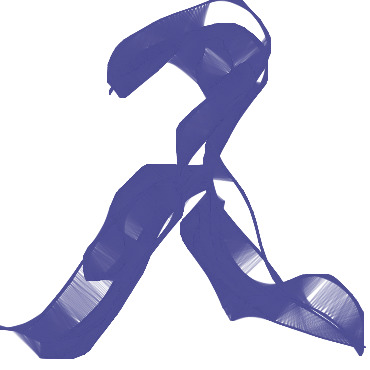
\includegraphics[height=18pt,clip]{../lambda.jpg}
       \end{minipage}
       \begin{minipage}{0.8\textwidth}
         {\footnotesize \textcopyright\ 2021 \href{https://williamdemeo.gitlab.io}{William DeMeo}. Based on work at \href{https://gitlab.com/ualib/ualib.gitlab.io}{https://gitlab.com/ualib/ualib.gitlab.io}.\\
Compiled with \texttt{xelatex} on \mydate\today\ at \currenttime.
}
       \end{minipage}}
   \renewcommand{\headrulewidth}{0pt}
}}





\ccsdesc[500]{Theory of computation~Constructive mathematics}
\ccsdesc[500]{Theory of computation~Type theory}
\ccsdesc[500]{Theory of computation~Logic and verification}
\ccsdesc[300]{Computing methodologies~Representation of mathematical objects}
\ccsdesc[300]{Theory of computation~Type structures}


\keywords{Universal algebra, Equational logic, Model theory, Dependent type theory, Formalization of mathematics, Agda, Proof assistant, Constructive mathematics}

\category{} %optional, e.g. invited paper

\relatedversion{hosted on arXiv}
\relatedversiondetails[linktext={arxiv.org/pdf/2101.10166}]{Extended Version}{https://arxiv.org/pdf/2101.10166}

\supplement{~\\ \textit{Documentation}: \ualibdotorg}%
\supplementdetails{Software}{https://gitlab.com/ualib/ualib.gitlab.io.git}

\acknowledgements{The author wishes to thank Cliff Bergman, Hyeyoung Shin, and Siva Somayyajula for supporting and contributing to this project, and \MartinEscardo for creating the \TypeTopology library and teaching a course on \href{https://www.cs.bham.ac.uk/~mhe/HoTT-UF-in-Agda-Lecture-Notes/index.html}{Univalent Foundations of Mathematics with Agda} at the \href{http://events.cs.bham.ac.uk/mgs2019/}{2019 Midlands Graduate School in Computing Science}. Of course, this work would not exist in its current form without the Agda 2 language by Ulf Norell.\footnote{Agda 2 is partially based on code from Agda 1 by Catarina Coquand and Makoto Takeyama, and from Agdalight by Ulf Norell and Andreas Abel.}}

\nolinenumbers %uncomment to disable line numbering

%\hideLIPIcs  %uncomment to remove references to LIPIcs series (logo, DOI, ...), e.g. when preparing a pre-final version to be uploaded to arXiv or another public repository

%Editor-only macros:: begin (do not touch as author)%%%%%%%%%%%%%%%%%%%%%%%%%%%%%%%%%%
\EventEditors{}
\EventNoEds{2}
\EventLongTitle{}
\EventShortTitle{}
\EventAcronym{}
\EventYear{2021}
\EventDate{Feb 16, 2021}
\EventLocation{}
\EventLogo{}
\SeriesVolume{0}
\ArticleNo{0}
%%%%%%%%%%%%%%%%%%%%%%%%%%%%%%%%%%%%%%%%%%%%%%%%%%%%%%

\begin{document}

\maketitle


\begin{abstract}
The Agda Universal Algebra Library (UALib) is a library of types and programs (theorems and proofs) we developed to formalize the foundations of universal algebra in dependent type theory using the Agda programming language and proof assistant. 
 The UALib includes a substantial collection of definitions, theorems, and proofs from universal algebra, equational logic, and model theory, and as such provides many examples that exhibit the power of inductive and dependent types for representing and reasoning about mathematical structures and equational theories. In this paper we describe some of the most important foundational types and assumptions of the UALib, and we discuss some of the problems that arose when developing it, as well as our solutions to these problems.
\end{abstract}

\newpage

\setcounter{tocdepth}{2}
\tableofcontents

\section{Introduction}\label{sec:introduction}

To support formalization in type theory of research level mathematics in universal algebra and related fields, we present the Agda Universal Algebra Library (\agdaualib), a software library containing formal statements and proofs of the core definitions and results of universal algebra. 
The \ualib is written in \agda~\cite{Norell:2009}, a programming language and proof assistant based on Martin-L\"of Type Theory that not only supports dependent and inductive types, as well as proof tactics for proving things about the objects that inhabit these types.

\subsection{Motivation}\label{sec:motivation}
%% \subsection{Vision and Goals}\label{vision-and-goals}
The seminal idea for the \agdaualib project was the observation that, on the one hand, a number of fundamental constructions in universal algebra can be defined recursively, and theorems about them proved by structural induction, while, on the other hand, inductive and dependent types make possible very precise formal representations of recursively defined objects, which often admit elegant constructive proofs of properties of such objects.  An important feature of such proofs in type theory is that they are total functional programs and, as such, they are computable, composable, and machine-verifiable.
%% These observations suggested that there would be much to gain from implementing universal algebra in a language, such as Martin-L\"of type theory, that features dependent and inductive types.

Finally, our own research experience has taught us that a proof assistant and programming language (like Agda), when equipped with specialized libraries and domain-specific tactics to automate the proof idioms of our field, can be an extremely powerful and effective asset. As such we believe that proof assistants and their supporting libraries will eventually become indispensable tools in the working mathematician's toolkit.


\subsection{Attributions and Contributions}\label{sec:contributions}
The mathematical results described in this paper have well known \emph{informal} proofs. Our main contribution is the formalization, mechanization, and verification of the statements and proofs of these results in dependent type theory using Agda.

Unless explicitly stated otherwise, the Agda source code described in this paper is due to the author, with the following caveat: the \ualib depends on the \typetopology library of \MartinEscardo~\cite{MHE}.  Each dependency is carefully accounted for and mentioned in this paper. For the sake of completeness and clarity, and to keep the paper mostly self-contained, we repeat some definitions from the \typetopology library, but in each instance we cite the original source.\footnote{In the \ualib, such instances occur only inside hidden modules that are never actually used, followed immediately by a statement that imports the code in question from its original source.}


\subsection{Organization of the paper}\label{sec:organization}

In this paper we limit ourselves to the presentation of the middle third of the \ualib, which includes types for representing homomorphisms, terms, and subalgebras. This limitation will allow us the space required to discuss some of the more interesting type theoretic and foundational issues that arise when developing a library of this kind and when attempting to represent advanced mathematical notions in type theory and formalize them in Agda.

This is the second installment of a three-part series of papers describing the \agdaualib. The first part is~\cite{DeMeo:2021-1} which covers relations, algebras, congruences, and quotients. The third part will cover free algebras, equational classes of algebras (i.e., varieties), and Birkhoff's HSP theorem.

The present paper is divided into three main parts, in \S\ref{sec:homomorphism-types}, \S\ref{sec:types-terms}, and 4.  The first of these introduces types representing \emph{homomorphisms} from one algebra to another, and presents a formal statement and proof of the first fundamental theorem about homomorphisms, known as the \emph{First Isomorphism Theorem}, as well as a version of the so-called \emph{Second Isomorphism Theorem}. This is followed by dependents type definitions for representing \emph{isomorphisms} and \emph{homomorphic images} of algebraic structures.

In Section~\ref{sec:types-terms} we define inductive types to represent \emph{terms} in a given signature and the \emph{term algebra}. It is here that we prove the \emph{absolute universality} (or \emph{initiality}) \emph{property} of the term algebra.  We define types that denote the interpretation of a term in an algebra type, called a \emph{term operation}, including the interpretation of terms in \emph{arbitrary products} of algebras (\S\ref{interpretation-of-terms-in-product-algebras}). The second part concludes with subsection~\ref{compatibility-of-terms} on the compatibility of terms with basic operations and congruence relations.

Section~\ref{sec:subalgebra-types} presents inductive and dependent types for representing subuniverses and subalgebras of a given algebra. Here we define an inductive type that represents the \emph{subuniverse generated by} \ab X, for a given predicate \ab X \as : \af{Pred} \af ∣ \ab 𝑨 \af ∣ \AgdaUnderscore,\footnote{As we learned in~\cite{DeMeo:2021-1}, such \ab X represents a subset of the domain of the algebra \ab 𝑨.} and we use this type to formalize a few basic subuniverse lemmas.  We also define types that pertain to arbitrary classes of algebras. In particular, in Subsection~\ref{sec:subalgebras} on subalgebras, we define a type that represents the assertion that a given algebra is a subalgebra of some member of a class of algebras.  Finally, the appendix~\S\ref{sec:univ-subalg} includes our generalization of Martin Escardo's use of \emph{univalence} for modeling subgroups.

\newcommand\otherparta{\textit{Part 1: equality, extensionality, truncation, and dependent types for relations and algebras}~\cite{DeMeo:2021-1}.}
\newcommand\otherpartb{\textit{Part 3: free algebras, equational classes, and Birkhoff's theorem}~\cite{DeMeo:2021-3}.}

\subsection{Resources}
We conclude this introduction with some pointers to helpful reference materials.
For the required background in Universal Algebra, we recommend the textbook by Clifford Bergman~\cite{Bergman:2012}.  For the type theory background, we recommend the HoTT Book~\cite{HoTT} and Escard\'o's \ufcourse~\cite{MHE}.

The following are informed the development of the \ualib and are highly recommended.
\begin{itemize}
\item \textit{\ufcourse}, \escardo~\cite{MHE}.
\item \href{http://www.cse.chalmers.se/~peterd/papers/DependentTypesAtWork.pdf}{\it Dependent Types at Work}, Bove and Dybjer~\cite{Bove:2009}.
\item \href{http://www.cse.chalmers.se/~ulfn/papers/afp08/tutorial.pdf}{\it Dependently Typed Programming in Agda}, Norell and Chapman~\cite{Norell:2008}.
\item \href{http://www.sciencedirect.com/science/article/pii/S1571066118300768}{\it Formalization of Universal Algebra in Agda}, Gunther, Gadea, Pagano~\cite{Gunther:2018}.
\item \href{https://plfa.github.io/}{\it Programming Languages Foundations in Agda}, Philip Wadler~\cite{Wadler:2020}.
\end{itemize}

More information about \agdaualib can be obtained from the following official sources.
\begin{itemize}
  \item \href{https://ualib.gitlab.io}{\texttt{ualib.org}} (the web site) documents every line of code in the library.
  \item \href{https://gitlab.com/ualib/ualib.gitlab.io}{\texttt{gitlab.com/ualib/ualib.gitlab.io}} (the source code) \agdaualib is open source.\footnote{License: \href{https://creativecommons.org/licenses/by-sa/4.0/}{Creative Commons Attribution-ShareAlike 4.0 International License.}}
  \item \emph{The Agda UALib}, \otherparta
  \item \emph{The Agda UALib}, \otherpartb
\end{itemize}
The first item links to the official \ualib html documentation which includes complete proofs of every theorem we mention here, and much more, including the Agda modules covered in the first and third installments of this series of papers on the \ualib.

Finally, readers will get much more out of reading the paper if they download the \agdaualib from \url{https://gitlab.com/ualib/ualib.gitlab.io}, install the library, and try it out for themselves.



%%% Local Variables:
%%% TeX-master: "ualib-part2-20210304.tex"
%%% End:

\newcommand\firstsentence[2]{This section describes certain key components of the #1 module of the \agdaualib.\footnote{For more details, see #2.}}





%%%%%%%%%%%%%%%%%%%%%%%%%%%%%%%%%%%%%%%%%%%%%%%%%%%%%%%%%%%%%%%%%%%%%%%%%%%%%%%%%%%%%%%%
%%%%%%%%%%%%%%%%%%%%%%%%%%%%%%%%%%%%%%%%%%%%%%%%%%%%%%%%%%%%%%%%%%%%%%%%%%%%%%%%%%%%%%%%
%%%%%%%%%%%%%%%%%%%%%%%%%%%%%%%%%%%%%%%%%%%%%%%%%%%%%%%%%%%%%%%%%%%%%%%%%%%%%%%%%%%%%%%%
% - [Prelude](Prelude.html)
\section{Agda Prelude}\label{sec:agda-prelude}

\subsection{Universes and dependent types}\label{preliminaries}\firstsentence{\ualibPreliminaries}{\urlPreliminaries}
% -*- TeX-master: "ualib-part1.tex" -*-
%%% Local Variables: 
%%% mode: latex
%%% TeX-engine: 'xetex
%%% End:
Here we define or import the basic types of \defn{Martin-Löf type theory} (\mltt).  Although this is standard stuff, we take this opportunity to highlight aspects of the \ualib syntax that may differ from that of ``standard Agda.''

\subsubsection{Logical foundations}\label{sec:logical-foundations}
% Mainly for the benefit of readers who are not yet proficient in Agda or type theory, we briefly describe the type theoretic foundations of the \ualib. 
The \agdaualib is based on a type theory that is the same or very close to the one on which on which Martín Escardó's \typetopology Agda library is based. We don't discuss \mltt in great detail here because there are already nice and freely available resources covering the theory. (See, for example, the section \href{https://www.cs.bham.ac.uk/~mhe/HoTT-UF-in-Agda-Lecture-Notes/HoTT-UF-Agda.html\#mlttinagda}{A spartan Martin-Löf type theory} of the lecture notes by Escard\'o~\cite{MHE}, the \href{https://ncatlab.org/nlab/show/Martin-L\%C3\%B6f+dependent+type+theory}{ncatlab entry on Martin-Löf dependent type theory}, or the HoTT Book~\cite{HoTT}.)

The objects and assumptions that form the foundation of \mltt are few.  There are the \defn{primitive types} (\ad 𝟘, \ad 𝟙, and \ad ℕ, denoting the empty type, one-element type, and natural numbers), the \defn{type formers} (\ad +, \ad Π, \ad Σ, \ad{Id}, denoting \defn{binary sum}, \defn{product}, \defn{sum}, and the \defn{identity} type). Each of these type formers is defined by a \defn{type forming rule} which specifies how that type is constructed. Lastly, we have an infinite collection of \defn{type universes} (types of types) and \defn{universe variables} to denote them. Following Escardó, we denote universes in the \ualib by upper-case calligraphic letters from the second half of the English alphabet; to be precise, these are \ab 𝓞, \ab 𝓠, \ab 𝓡, …, \ab 𝓧, \ab 𝓨, \ab 𝓩.\footnote{We avoid using \ab 𝓟 as a universe variable because in the \typetopology library \ab 𝓟 denotes a powerset type.}

That's all. There are no further axioms or logical deduction (proof derivation) rules needed for the foundation of \mltt that we take as the starting point of the \agdaualib. The logical semantics come from the \href{https://ncatlab.org/nlab/show/propositions+as+types}{propositions-as-types correspondence}~\cite{nlab:propositions_as_types}: propositions and predicates are represented by types and the inhabitants of these types are the proofs of the propositions and predicates. As such, proofs are constructed using the type forming rules. In other words, the type forming rules \emph{are} the proof derivation rules.

To this foundation, we add certain \textit{extensionality principles} when and were we need them.  These will be developed as we progress.  However, classical axioms such as the \href{https://ncatlab.org/nlab/show/axiom+of+choice}{\textit{Axiom of Choice}} or the \href{https://ncatlab.org/nlab/show/excluded+middle}{\textit{Law of the Excluded Middle}} are not needed and are not assumed anywhere in the library.  In that sense, all theorems and proofs in the \ualib are \href{https://ncatlab.org/nlab/show/constructive+mathematics}{\textit{constructive}} (as defined, e.g., in~\cite{nlab:constructive_mathematics}).

A few specific instances (e.g., the proof of the Noether isomorphism theorems and Birkhoff's HSP theorem) require certain \textit{truncation} assumptions. In such cases, the theory is not \href{https://ncatlab.org/nlab/show/predicative+mathematics}{\textit{predicative}} (as defined, e.g., in~\cite{nlab:predicative_mathematics}). These instances are always clearly identified.




\paragraph*{Specifying logical foundations in Agda}
An Agda program typically begins by setting some options and by importing types from existing Agda libraries.
Options are specified with the \AgdaKeyword{OPTIONS} \emph{pragma} and control the way Agda behaves by, for example, specifying the logical axioms and deduction rules we wish to assume when the program is type-checked to verify its correctness. Every Agda program in the \ualib begins with the following line.
\ccpad
\begin{code}[number=code:options]
\>[0]\AgdaSymbol{\{-\#}\AgdaSpace{}%
\AgdaKeyword{OPTIONS}\AgdaSpace{}%
\AgdaPragma{--without-K}\AgdaSpace{}%
\AgdaPragma{--exact-split}\AgdaSpace{}%
\AgdaPragma{--safe}\AgdaSpace{}%
\AgdaSymbol{\#-\}}\<%
\end{code}
\ccpad
These options control certain foundational assumptions that Agda makes when type-checking the program to verify its correctness.
\begin{itemize}
\item \AgdaPragma{--without-K} disables \axiomk; see~\cite{agdaref-axiomk};
\item \AgdaPragma{--exact-split} makes Agda accept only definitions that are \emph{judgmental} equalities; see~\cite{agdatools-patternmatching};
\item \AgdaPragma{--safe} ensures that nothing is postulated outright---every non-\mltt axiom has to be an explicit assumption (e.g., an argument to a function or module); see~\cite{agdaref-safeagda} and~\cite{agdatools-patternmatching}.
\end{itemize}
%% \end{enumerate}
Throughout this paper we take assumptions 1--3 for granted without mentioning them explicitly.


\subsubsection{Agda Modules}\label{sec:agda-modules}
The \ak{OPTIONS} pragma is usually followed by the start of a module.  For example, the \ualibhtml{Overture.Preliminaries} module begins with the following line.
\ccpad
\begin{code}%
\>[0]\AgdaKeyword{module}\AgdaSpace{}%
\AgdaModule{Overture.Preliminaries}\AgdaSpace{}%
\AgdaKeyword{where}\<%
\end{code}
\ccpad
Sometimes we want to declare parameters that will be assumed throughout the module.  For instance, when working with algebras, we often assume they come from a particular fixed signature, and this signature is something we could fix as a parameter at the start of a module. Thus, we might start an \defn{anonymous submodule} of the main module with a line like\footnote{The \af{Signature} type will be defined in Section~\ref{sec:oper-sign}.}
\ccpad
\begin{code}%
\>[0]\AgdaKeyword{module}\AgdaSpace{}%
\AgdaUnderscore\AgdaSpace{}%
\AgdaSymbol{\{}\AgdaBound{𝑆}\AgdaSpace{}%
\AgdaSymbol{:}\AgdaSpace{}%
\AgdaFunction{Signature}\AgdaSpace{}%
\AgdaBound{𝓞}\AgdaSpace{}%
\AgdaBound{𝓥}\AgdaSymbol{\}}\AgdaSpace{}%
\AgdaKeyword{where}\<%
\end{code}
\ccpad
Such a module is called \emph{anonymous} because an underscore appears in place of a module name. Agda determines where a submodule ends by indentation.  This can take some getting used to, but after a short time it will feel very natural. The main module of a file must have the same name as the file, without the \texttt{.agda} or \texttt{.lagda} file extension.  The code inside the main module is not indented. Submodules are declared inside the main module and code inside these submodules must be indented to a fixed column.  As long as the code is indented, Agda considers it part of the submodule.  A submodule is exited as soon as a nonindented line of code appears.



\subsubsection{Universes in Agda}\label{universes}

For the very small amount of background we require about the notion of \emph{type universe} (or \emph{level}), we refer the reader to the brief \href{https://agda.readthedocs.io/en/v2.6.1.3/language/universe-levels.html}{section
on universe-levels} in the \href{https://agda.readthedocs.io/en/v2.6.1.3/language/universe-levels.html}{Agda
documentation}.\footnote{See \url{https://agda.readthedocs.io/en/v2.6.1.3/language/universe-levels.html}.}

Throughout the \agdaualib we use many of the nice tools that Martín Escardó has developed and made available in the \typetopology
repository of Agda code for the \emph{Univalent Foundations} of mathematics.\footnote{%
Escardó has written an outstanding set of notes called
\href{https://www.cs.bham.ac.uk/~mhe/HoTT-UF-in-Agda-Lecture-Notes/index.html}{Introduction to Univalent Foundations of Mathematics with Agda}, which we highly recommend to anyone looking for more details than we provide
here about \mltt and Univalent Foundations/HoTT in Agda.~\cite{MHE}.}
The first of these is the \am{Universes} module which we import as follows.
\ccpad
\begin{code}%
\>[0]\AgdaKeyword{open}\AgdaSpace{}%
\AgdaKeyword{import}\AgdaSpace{}%
\AgdaModule{Universes}\AgdaSpace{}%
\AgdaKeyword{public}\<%
\end{code}
\ccpad
Since we use the \ak{public} directive, the \am{Universes} module will be available to all modules that import
the present module (\ualibhtml{Overture.Preliminaries}). This module declares symbols used to denote universes. As mentioned, we adopt Escardó's convention of denoting universes by capital calligraphic letters, and most of the ones we use are already declared in \am{Universes}; those that are not are declared as follows.
\ccpad
\begin{code}%
\>[0]\AgdaKeyword{variable}\AgdaSpace{}%
\AgdaGeneralizable{𝓞}\AgdaSpace{}%
\AgdaGeneralizable{𝓧}\AgdaSpace{}%
\AgdaGeneralizable{𝓨}\AgdaSpace{}%
\AgdaGeneralizable{𝓩}\AgdaSpace{}%
\AgdaSymbol{:}\AgdaSpace{}%
\AgdaPostulate{Universe}\<%
\end{code}
\scpad

The \am{Universes} module also provides alternative syntax for the primitive operations on universes that Agda supports. Specifically, the \af ̇ operator maps a universe level \ab 𝓤 to the type \ad{Set}~\ab 𝓤, and the latter has type \apt{Set}~(\apr{lsuc}~\ab 𝓤). The Agda level \apr{lzero} is renamed \apr{𝓤₀}, so \apr{𝓤₀}\af ̇ is an alias for \apr{Set}~\apr{lzero}. Thus, \ab 𝓤\af ̇ is simply an alias for \apr{Set}~\ab 𝓤, and we have \apr{Set}~\ab 𝓤~\as :~\apr{Set}~(\apr{lsuc}~\ab 𝓤). Finally, \apr{Set}~(\apr{lsuc}~\apr{lzero}) is equivalent to \apr{Set}~\apr{𝓤₀}\af ⁺, which we (and Escardó) denote by \apr{𝓤₀}\af ⁺\af ̇.

% The following dictionary translates between standard Agda syntax and Type Topology/UALib notation.

% \begin{Shaded}
% \begin{Highlighting}[]
% \NormalTok{Agda              Type Topology/UALib}
% \NormalTok{====              ===================}
% \NormalTok{Level             Universe}
% \NormalTok{lzero             𝓤₀}
% \NormalTok{𝓤 }\OtherTok{:}\NormalTok{ Level         𝓤 }\OtherTok{:}\NormalTok{ Universe}
% \DataTypeTok{Set}\NormalTok{ lzero         𝓤₀ ̇}
% \DataTypeTok{Set}\NormalTok{ 𝓤             𝓤 ̇}
% \NormalTok{lsuc lzero        𝓤₀ ⁺}
% \NormalTok{lsuc 𝓤            𝓤 ⁺}
% \DataTypeTok{Set} \OtherTok{(}\NormalTok{lsuc lzero}\OtherTok{)}\NormalTok{  𝓤₀ ⁺ ̇}
% \DataTypeTok{Set} \OtherTok{(}\NormalTok{lsuc 𝓤}\OtherTok{)}\NormalTok{      𝓤 ⁺ ̇}
% \NormalTok{Setω              𝓤ω}
% \end{Highlighting}
% \end{Shaded}

To justify the introduction of this somewhat nonstandard notation for universe levels, Escardó points out that the Agda library uses \apr{Level} for universes (so what we write as \ab 𝓤\af ̇ is written \apr{Set}~\ab 𝓤 in standard Agda), but in univalent mathematics the types in \ab 𝓤\af ̇ need not be sets, so the standard Agda notation can be
a bit confusing, especially to newcomers.

There will be many occasions calling for a type living in a universe at the level that is the least upper bound of two universe levels, say, \ab 𝓤 and \ab 𝓥. The universe level \ab 𝓤~\apr ⊔~\ab 𝓥\af denotes this least upper bound. Here \apr ⊔ is an Agda primitive designed for precisely this purpose.


\subsubsection{Dependent types}\label{sec:dependent-types}

\newcommand\FstUnder{\AgdaOperator{\AgdaFunction{∣\AgdaUnderscore{}∣}}\xspace}
\newcommand\SndUnder{\AgdaOperator{\AgdaFunction{∥\AgdaUnderscore{}∥}}\xspace}
% Convenient notations for the first and second projections out of a product are \FstUnder and \SndUnder, respectively. However, to improve readability or to avoid notation clashes with other modules, we sometimes use more standard alternatives, such as \AgdaFunction{pr₁} and \AgdaFunction{pr₂}, or \AgdaFunction{fst} and \AgdaFunction{snd}, or some combination of these. The definitions are standard so we omit them.\footnote{For details see~\cite{DeMeo:2021} or \ualiburl{Overture.Preliminaries}.}








\paragraph*{Sigma types (dependent pairs)} %\label{ssec:dependent-pairs}

Given universes \ab 𝓤 and \ab 𝓥, a type \ab{A} \as : \ab 𝓤\af ̇, and a type family \ab{B}~\as :~\ab A~\as →~\ab 𝓥\af ̇, the \defn{Sigma type} (or \defn{dependent pair type}, or \defn{dependent product type}) is denoted by \ar{Σ}~\abt{x}{A} ,~\ab B~\ab x and generalizes the Cartesian product \ab A~\af ×~\ab B by allowing the type \ab{B x} of the second argument of the ordered pair (\ab x \af , \ab y) to depend on the value \ab{x} of the first. That is, an inhabitant of the type \ar{Σ}~\abt{x}{A}~,~\ab B~\ab x is a pair (\ab{x}~\af ,~\ab y) such that \abt{x}{A} and \abt{y}{B x}.

The dependent product type is defined in the \typetopology in a standard way. For pedagogical purposes we repeat the definition here.\footnote{In the \ualib we put such redundant definitions inside ``hidden'' modules so that they doesn't conflict with the original definitions which we import and use. It may seem odd to define something in a hidden module only to import and use an alternative definition, but we do this in order to exhibit all of the types on which the \ualib depends while ensuring that this cannot be misinterpreted as a claim to originality.}
\ccpad
\begin{code}%
\>[1]\AgdaKeyword{record}\AgdaSpace{}%
\AgdaRecord{Σ}\AgdaSpace{}%
\AgdaSymbol{\{}\AgdaBound{𝓤}\AgdaSpace{}%
\AgdaBound{𝓥}\AgdaSymbol{\}}\AgdaSpace{}%
\AgdaSymbol{\{}\AgdaBound{A}\AgdaSpace{}%
\AgdaSymbol{:}\AgdaSpace{}%
\AgdaBound{𝓤}\AgdaSpace{}%
\AgdaOperator{\AgdaFunction{̇}}\AgdaSpace{}%
\AgdaSymbol{\}}\AgdaSpace{}%
\AgdaSymbol{(}\AgdaBound{B}\AgdaSpace{}%
\AgdaSymbol{:}\AgdaSpace{}%
\AgdaBound{A}\AgdaSpace{}%
\AgdaSymbol{→}\AgdaSpace{}%
\AgdaBound{𝓥}\AgdaSpace{}%
\AgdaOperator{\AgdaFunction{̇}}\AgdaSpace{}%
\AgdaSymbol{)}\AgdaSpace{}%
\AgdaSymbol{:}\AgdaSpace{}%
\AgdaBound{𝓤}\AgdaSpace{}%
\AgdaOperator{\AgdaPrimitive{⊔}}\AgdaSpace{}%
\AgdaBound{𝓥}\AgdaSpace{}%
\AgdaOperator{\AgdaFunction{̇}}%
\>[53]\AgdaKeyword{where}\<%
\\
\>[1][@{}l@{\AgdaIndent{0}}]%
\>[2]\AgdaKeyword{constructor}\AgdaSpace{}%
\AgdaOperator{\AgdaInductiveConstructor{\AgdaUnderscore{},\AgdaUnderscore{}}}\<%
\\
%
\>[2]\AgdaKeyword{field}\<%
\\
\>[2][@{}l@{\AgdaIndent{0}}]%
\>[3]\AgdaField{pr₁}\AgdaSpace{}%
\AgdaSymbol{:}\AgdaSpace{}%
\AgdaBound{A}\<%
\\
%
\>[3]\AgdaField{pr₂}\AgdaSpace{}%
\AgdaSymbol{:}\AgdaSpace{}%
\AgdaBound{B}\AgdaSpace{}%
\AgdaField{pr₁}\<%
\end{code}
\ccpad
Agda's default syntax for this type is \AgdaRecord{Σ}\sP{3}\AgdaSymbol{λ}(\ab x\sP{3}꞉\sP{3}\ab A)\sP{3}\as →\sP{3}\ab B, but we prefer the notation \AgdaRecord{Σ}~\abt{x}{A}~,~\ab B, which is closer to the standard syntax described in the preceding paragraph. Fortunately, the \typetopology library makes the preferred notation available with the following type definition and \ak{syntax} declaration (see~\cite[Σ types]{MHE}).\footnote{\label{fncolon}\textbf{Attention!} The symbol \af ꞉ that appears in the special syntax defined here for the \AgdaFunction{Σ} type, and below for the \af{Π} type, is not the ordinary colon; rather, it is the symbol obtained by typing \texttt{\textbackslash{}:4} in \agdatwomode.} 
\ccpad
\begin{code}%
\>[1]\AgdaFunction{-Σ}\AgdaSpace{}%
\AgdaSymbol{:}\AgdaSpace{}%
\AgdaSymbol{\{}\AgdaBound{𝓤}\AgdaSpace{}%
\AgdaBound{𝓥}\AgdaSpace{}%
\AgdaSymbol{:}\AgdaSpace{}%
\AgdaPostulate{Universe}\AgdaSymbol{\}}\AgdaSpace{}%
\AgdaSymbol{(}\AgdaBound{A}\AgdaSpace{}%
\AgdaSymbol{:}\AgdaSpace{}%
\AgdaBound{𝓤}\AgdaSpace{}%
\AgdaOperator{\AgdaFunction{̇}}\AgdaSpace{}%
\AgdaSymbol{)}\AgdaSpace{}%
\AgdaSymbol{(}\AgdaBound{B}\AgdaSpace{}%
\AgdaSymbol{:}\AgdaSpace{}%
\AgdaBound{A}\AgdaSpace{}%
\AgdaSymbol{→}\AgdaSpace{}%
\AgdaBound{𝓥}\AgdaSpace{}%
\AgdaOperator{\AgdaFunction{̇}}\AgdaSpace{}%
\AgdaSymbol{)}\AgdaSpace{}%
\AgdaSymbol{→}\AgdaSpace{}%
\AgdaBound{𝓤}\AgdaSpace{}%
\AgdaOperator{\AgdaPrimitive{⊔}}\AgdaSpace{}%
\AgdaBound{𝓥}\AgdaSpace{}%
\AgdaOperator{\AgdaFunction{̇}}\<%
\\
%
\>[1]\AgdaFunction{-Σ}\AgdaSpace{}%
\AgdaBound{A}\AgdaSpace{}%
\AgdaBound{B}\AgdaSpace{}%
\AgdaSymbol{=}\AgdaSpace{}%
\AgdaRecord{Σ}\AgdaSpace{}%
\AgdaBound{B}\<%
\\
%
\\[\AgdaEmptyExtraSkip]%
%
\>[1]\AgdaKeyword{syntax}\AgdaSpace{}%
\AgdaFunction{-Σ}\AgdaSpace{}%
\AgdaBound{A}\AgdaSpace{}%
\AgdaSymbol{(λ}\AgdaSpace{}%
\AgdaBound{x}\AgdaSpace{}%
\AgdaSymbol{→}\AgdaSpace{}%
\AgdaBound{B}\AgdaSymbol{)}\AgdaSpace{}%
\AgdaSymbol{=}\AgdaSpace{}%
\AgdaFunction{Σ}\AgdaSpace{}%
\AgdaBound{x}\AgdaSpace{}%
\AgdaFunction{꞉}\AgdaSpace{}%
\AgdaBound{A}\AgdaSpace{}%
\AgdaFunction{,}\AgdaSpace{}%
\AgdaBound{B}\<%
\end{code}
\scpad
% \textbf{WARNING!} The symbol \af ꞉ is not the same as \as : despite how similar they may look. The correct colon in the expression \ar{Σ}~\ab x~\af ꞉~\ab A~\af ,~\ab y, above is obtained by typing \texttt{\textbackslash{}:4} in \agdamode.

A special case of the Sigma type is the one in which the type \ab{B} doesn't depend on \ab{A}. This is the usual Cartesian product, defined in Agda as follows.
\ccpad
\begin{code}%
\>[1]\AgdaOperator{\AgdaFunction{\AgdaUnderscore{}×\AgdaUnderscore{}}}\AgdaSpace{}%
\AgdaSymbol{:}\AgdaSpace{}%
\AgdaGeneralizable{𝓤}\AgdaSpace{}%
\AgdaOperator{\AgdaFunction{̇}}\AgdaSpace{}%
\AgdaSymbol{→}\AgdaSpace{}%
\AgdaGeneralizable{𝓥}\AgdaSpace{}%
\AgdaOperator{\AgdaFunction{̇}}\AgdaSpace{}%
\AgdaSymbol{→}\AgdaSpace{}%
\AgdaGeneralizable{𝓤}\AgdaSpace{}%
\AgdaOperator{\AgdaPrimitive{⊔}}\AgdaSpace{}%
\AgdaGeneralizable{𝓥}\AgdaSpace{}%
\AgdaOperator{\AgdaFunction{̇}}\<%
\\
%
\>[1]\AgdaBound{A}\AgdaSpace{}%
\AgdaOperator{\AgdaFunction{×}}\AgdaSpace{}%
\AgdaBound{B}\AgdaSpace{}%
\AgdaSymbol{=}\AgdaSpace{}%
\AgdaFunction{Σ}\AgdaSpace{}%
\AgdaBound{x}\AgdaSpace{}%
\AgdaFunction{꞉}\AgdaSpace{}%
\AgdaBound{A}\AgdaSpace{}%
\AgdaFunction{,}\AgdaSpace{}%
\AgdaBound{B}\<%
\end{code}





\paragraph*{Pi types (dependent functions)} %\label{ssec:dependent-functions}
Given universes \ab 𝓤 and \ab 𝓥, a type \ab{A} \as : \ab 𝓤\af ̇, and a type family \ab{B}~\as :~\ab A~\as →~\ab 𝓥\af ̇, the \defn{Pi type} (or \defn{dependent function type}) is denoted by \ar Π~\abt{x}{A} ,~\ab B~\ab x and generalizes the function type \ab A~\as →~\ab B by letting the type \ab B~\ab x of the codomain depend on the value \ab x of the domain type. The dependent function type is defined in the \typetopology in a standard way.  For the reader's benefit, however, we repeat the definition here.  (In the \ualib this definition is included in a named or ``hidden'' module.)
\ccpad
\begin{code}%
\>[1]\AgdaFunction{Π}\AgdaSpace{}%
\AgdaSymbol{:}\AgdaSpace{}%
\AgdaSymbol{\{}\AgdaBound{A}\AgdaSpace{}%
\AgdaSymbol{:}\AgdaSpace{}%
\AgdaBound{𝓤}\AgdaSpace{}%
\AgdaOperator{\AgdaFunction{̇}}\AgdaSpace{}%
\AgdaSymbol{\}}\AgdaSpace{}%
\AgdaSymbol{(}\AgdaBound{A}\AgdaSpace{}%
\AgdaSymbol{:}\AgdaSpace{}%
\AgdaBound{A}\AgdaSpace{}%
\AgdaSymbol{→}\AgdaSpace{}%
\AgdaBound{𝓦}\AgdaSpace{}%
\AgdaOperator{\AgdaFunction{̇}}\AgdaSpace{}%
\AgdaSymbol{)}\AgdaSpace{}%
\AgdaSymbol{→}\AgdaSpace{}%
\AgdaBound{𝓤}\AgdaSpace{}%
\AgdaOperator{\AgdaPrimitive{⊔}}\AgdaSpace{}%
\AgdaBound{𝓦}\AgdaSpace{}%
\AgdaOperator{\AgdaFunction{̇}}\<%
\\
%
\>[1]\AgdaFunction{Π}\AgdaSpace{}%
\AgdaSymbol{\{}\AgdaBound{A}\AgdaSymbol{\}}\AgdaSpace{}%
\AgdaBound{A}\AgdaSpace{}%
\AgdaSymbol{=}\AgdaSpace{}%
\AgdaSymbol{(}\AgdaBound{x}\AgdaSpace{}%
\AgdaSymbol{:}\AgdaSpace{}%
\AgdaBound{A}\AgdaSymbol{)}\AgdaSpace{}%
\AgdaSymbol{→}\AgdaSpace{}%
\AgdaBound{A}\AgdaSpace{}%
\AgdaBound{x}\<%
\end{code}
\ccpad
To make the syntax for \af{Π} conform to the standard notation for Pi types, \escardo uses the same trick as the one used above for Sigma types.\cref{fncolon}
\ccpad
\begin{code}
\>[1]\AgdaFunction{-Π}\AgdaSpace{}%
\AgdaSymbol{:}\AgdaSpace{}%
\AgdaSymbol{(}\AgdaBound{A}\AgdaSpace{}%
\AgdaSymbol{:}\AgdaSpace{}%
\AgdaBound{𝓤}\AgdaSpace{}%
\AgdaOperator{\AgdaFunction{̇}}\AgdaSpace{}%
\AgdaSymbol{)(}\AgdaBound{B}\AgdaSpace{}%
\AgdaSymbol{:}\AgdaSpace{}%
\AgdaBound{A}\AgdaSpace{}%
\AgdaSymbol{→}\AgdaSpace{}%
\AgdaBound{𝓦}\AgdaSpace{}%
\AgdaOperator{\AgdaFunction{̇}}\AgdaSpace{}%
\AgdaSymbol{)}\AgdaSpace{}%
\AgdaSymbol{→}\AgdaSpace{}%
\AgdaBound{𝓤}\AgdaSpace{}%
\AgdaOperator{\AgdaPrimitive{⊔}}\AgdaSpace{}%
\AgdaBound{𝓦}\AgdaSpace{}%
\AgdaOperator{\AgdaFunction{̇}}\<%
\\
%
\>[1]\AgdaFunction{-Π}\AgdaSpace{}%
\AgdaBound{A}\AgdaSpace{}%
\AgdaBound{B}\AgdaSpace{}%
\AgdaSymbol{=}\AgdaSpace{}%
\AgdaFunction{Π}\AgdaSpace{}%
\AgdaBound{B}\<%
\\
%
\\[\AgdaEmptyExtraSkip]%
\>[1]\AgdaKeyword{syntax}\AgdaSpace{}%
\AgdaFunction{-Π}\AgdaSpace{}%
\AgdaBound{A}\AgdaSpace{}%
\AgdaSymbol{(λ}\AgdaSpace{}%
\AgdaBound{x}\AgdaSpace{}%
\AgdaSymbol{→}\AgdaSpace{}%
\AgdaBound{b}\AgdaSymbol{)}\AgdaSpace{}%
\AgdaSymbol{=}\AgdaSpace{}%
\AgdaFunction{Π}\AgdaSpace{}%
\AgdaBound{x}\AgdaSpace{}%
\AgdaFunction{꞉}\AgdaSpace{}%
\AgdaBound{A}\AgdaSpace{}%
\AgdaFunction{,}\AgdaSpace{}%
\AgdaBound{b}\<%
\end{code}
\ccpad
Once we have studied the types, defined in the \typetopology library and repeated here for illustration purposes, the original definitions are imported like so.
\ccpad
\begin{code}%
\>[0]\AgdaKeyword{open}\AgdaSpace{}%
\AgdaKeyword{import}\AgdaSpace{}%
\AgdaModule{Sigma-Type}\AgdaSpace{}%
\AgdaKeyword{public}\<%
\\
\>[0]\AgdaKeyword{open}\AgdaSpace{}%
\AgdaKeyword{import}\AgdaSpace{}%
\AgdaModule{MGS-MLTT}\AgdaSpace{}%
\AgdaKeyword{using}\AgdaSpace{}%
\AgdaSymbol{(}\AgdaFunction{pr₁}\AgdaSymbol{;}\AgdaSpace{}%
\AgdaFunction{pr₂}\AgdaSymbol{;}\AgdaSpace{}%
\AgdaOperator{\AgdaFunction{\AgdaUnderscore{}×\AgdaUnderscore{}}}\AgdaSymbol{;}\AgdaSpace{}%
\AgdaFunction{-Σ}\AgdaSymbol{;}\AgdaSpace{}%
\AgdaFunction{Π}\AgdaSymbol{;}\AgdaSpace{}%
\AgdaFunction{-Π}\AgdaSymbol{)}\AgdaSpace{}
\AgdaKeyword{public}\<%
\end{code}
%\ccpad
%We use the  directive so that the types are available to all modules that import the present module.
% the \ualibhtml{Overture.Preliminaries} module.

\paragraph*{Projection notation}

The definition of \ar Σ (and thus \af ×) includes the fields  \af{pr₁} and \af{pr₂} representing the first and second projections out of the product.  Sometimes we prefer to denote these projections by \af{∣\_∣} and \af{∥\_∥}, respectively. However, for emphasis or readability we alternate between these and the following standard notations: \af{pr₁} and \af{fst} for the first projection, \af{pr₂} and \af{snd} for the second.  We define these alternative notations for projections as follows.
% \footnote{We have made a concerted effort to avoid duplicating types that are already provided elsewhere, such as the \typetopology library.  We occasionally repeat the definitions of such types for pedagogical purposes, but we always import and work with the original definitions in order to make the sources known and to credit the original authors.}
\ccpad
\begin{code}%
\>[0]\AgdaKeyword{module}\AgdaSpace{}%
\AgdaModule{\AgdaUnderscore{}}\AgdaSpace{}%
\AgdaSymbol{\{}\AgdaBound{𝓤}\AgdaSpace{}%
\AgdaSymbol{:}\AgdaSpace{}%
\AgdaPostulate{Universe}\AgdaSymbol{\}\{}\AgdaBound{A}\AgdaSpace{}%
\AgdaSymbol{:}\AgdaSpace{}%
\AgdaBound{𝓤}\AgdaSpace{}%
\AgdaOperator{\AgdaFunction{̇}}\AgdaSpace{}%
\AgdaSymbol{\}\{}\AgdaBound{B}\AgdaSpace{}%
\AgdaSymbol{:}\AgdaSpace{}%
\AgdaBound{A}\AgdaSpace{}%
\AgdaSymbol{→}\AgdaSpace{}%
\AgdaGeneralizable{𝓥}\AgdaSpace{}%
\AgdaOperator{\AgdaFunction{̇}}\AgdaSymbol{\}}\AgdaSpace{}%
\AgdaKeyword{where}\<%
\\
%
\\[\AgdaEmptyExtraSkip]%
\>[0][@{}l@{\AgdaIndent{0}}]%
\>[1]\AgdaOperator{\AgdaFunction{∣\AgdaUnderscore{}∣}}\AgdaSpace{}%
\AgdaFunction{fst}\AgdaSpace{}%
\AgdaSymbol{:}\AgdaSpace{}%
\AgdaRecord{Σ}\AgdaSpace{}%
\AgdaBound{B}\AgdaSpace{}%
\AgdaSymbol{→}\AgdaSpace{}%
\AgdaBound{A}\<%
\\
%
\>[1]\AgdaOperator{\AgdaFunction{∣}}\AgdaSpace{}%
\AgdaBound{x}\AgdaSpace{}%
\AgdaOperator{\AgdaInductiveConstructor{,}}\AgdaSpace{}%
\AgdaBound{y}\AgdaSpace{}%
\AgdaOperator{\AgdaFunction{∣}}\AgdaSpace{}%
\AgdaSymbol{=}\AgdaSpace{}%
\AgdaBound{x}\<%
\\
%
\>[1]\AgdaFunction{fst}\AgdaSpace{}%
\AgdaSymbol{(}\AgdaBound{x}\AgdaSpace{}%
\AgdaOperator{\AgdaInductiveConstructor{,}}\AgdaSpace{}%
\AgdaBound{y}\AgdaSymbol{)}\AgdaSpace{}%
\AgdaSymbol{=}\AgdaSpace{}%
\AgdaBound{x}\<%
\\
%
\\[\AgdaEmptyExtraSkip]%
%
\>[1]\AgdaOperator{\AgdaFunction{∥\AgdaUnderscore{}∥}}\AgdaSpace{}%
\AgdaFunction{snd}\AgdaSpace{}%
\AgdaSymbol{:}\AgdaSpace{}%
\AgdaSymbol{(}\AgdaBound{z}\AgdaSpace{}%
\AgdaSymbol{:}\AgdaSpace{}%
\AgdaRecord{Σ}\AgdaSpace{}%
\AgdaBound{B}\AgdaSymbol{)}\AgdaSpace{}%
\AgdaSymbol{→}\AgdaSpace{}%
\AgdaBound{B}\AgdaSpace{}%
\AgdaSymbol{(}\AgdaFunction{pr₁}\AgdaSpace{}%
\AgdaBound{z}\AgdaSymbol{)}\<%
\\
%
\>[1]\AgdaOperator{\AgdaFunction{∥}}\AgdaSpace{}%
\AgdaBound{x}\AgdaSpace{}%
\AgdaOperator{\AgdaInductiveConstructor{,}}\AgdaSpace{}%
\AgdaBound{y}\AgdaSpace{}%
\AgdaOperator{\AgdaFunction{∥}}\AgdaSpace{}%
\AgdaSymbol{=}\AgdaSpace{}%
\AgdaBound{y}\<%
\\
%
\>[1]\AgdaFunction{snd}\AgdaSpace{}%
\AgdaSymbol{(}\AgdaBound{x}\AgdaSpace{}%
\AgdaOperator{\AgdaInductiveConstructor{,}}\AgdaSpace{}%
\AgdaBound{y}\AgdaSymbol{)}\AgdaSpace{}%
\AgdaSymbol{=}\AgdaSpace{}%
\AgdaBound{y}\<%
\end{code}
\ccpad
\textbf{Remarks}.
\begin{itemize}
\item We place these definitions (of \AgdaOperator{\AgdaFunction{∣\AgdaUnderscore{}∣}}, \AgdaFunction{fst}, \AgdaOperator{\AgdaFunction{∥\AgdaUnderscore{}∥}} and \AgdaFunction{snd}) inside an \defn{anonymous module}, which is a module that begins with the \ak{module} keyword followed by an underscore character (instead of a module name). The purpose is to move some of the postulated typing judgments---the ``parameters'' of the module (e.g., \ab 𝓤 \as : \AgdaPostulate{Universe})---out of the way so they don't obfuscate the definitions inside the module.  In library documentation, such as the present paper, we often omit such module directives. In contrast, the collection of html pages at \ualibdotorg, which is the most current and comprehensive documentation of the \ualib, omits nothing.
\item As the four definitions above make clear, multiple inhabitants of a single type (e.g., \AgdaOperator{\AgdaFunction{∣\AgdaUnderscore{}∣}} and \AgdaFunction{fst}) may be declared on the same line.
\end{itemize}

\subsection{Equality}\label{equality}\firstsentence{\ualibEquality}{\urlEquality}
% -*- TeX-master: "ualib-part1.tex" -*-
%%% Local Variables: 
%%% mode: latex
%%% TeX-engine: 'xetex
%%% End:
\subsubsection{Definitional equality}\label{sec:defin-equal}
Here we discuss what is probably the most important type in \mltt. It is called \defn{definitional equality}. This concept is most understood, at least heuristically, with the following slogan: ``Definitional equality is the substitution-preserving equivalence relation generated by definitions.''
We will make this precise below, but first let us quote from a primary source. Per Martin-L\"of offers the following definition in~\cite[\S1.11]{MR0387009} (italics added):\footnote{The \defn{definiendum} is the left-hand side of a defining equation, the \defn{definiens} is the right-hand side.\\ For readers who have never generated an equivalence relation: the \defn{reflexive closure} of \ab R \af ⊆ \ab A \ad × \ab A is the union of \ab R and all pairs of the form (\ab a , \ab a); the \defn{symmetric closure} is the union of \ab R and its inverse \{(\ab y , \ab x) : (\ab x , \ab y) ∈ \ab R\}; we leave it to the reader to come up with the correct definition of transitive closure.}
\begin{quote}
  \defn{Definitional equality} is defined to be the equivalence relation, that is, reflexive, symmetric and transitive relation, which is generated by the principles that a definiendum is always definitionally equal to its definiens and that definitional equality is preserved under substitution.
\end{quote}
To be sure we understand what this means, let $:=$ denote the relation with respect to which $x$ is related to $y$ (denoted $x := y$) if and only if $y$ \emph{is the definition of} $x$.  Then the definitional equality relation \ad ≡ is the reflexive, symmetric, transitive, substitutive closure of $:=$. By \defn{subsitutive closure} we mean closure under the following \defn{substitution rule}.
% \{\ab A \as : \ab 𝓤\af ̇\}\{\ab B \as : \ab A \as → \ab 𝓦\af ̇\}\{\ab x \abt{y}{A}\} \as → \ab x \ad ≡ \ab y \as → \ab B \ab x \ad ≡ \ab B \ab y\\[4pt]
\vskip3mm\hskip1cm \infer[(subst)]{\ab B~\ab x~\ad ≡~\ab B~\ab y}{\{\ab A~\as :~\ab 𝓤\af ̇\}~\{\ab B~\as :~\ab A~\as →~\ab 𝓦\af ̇\}~\{\ab x~\abt{y}{A}\}  & \ab x~\ad ≡~\ab y}\\[-5pt]


% In~\cite[\S1.11, page 85]{MR0387009}, Per Martin-L\"of describes definitional equality as follows:
% \begin{quote}
% ``Definitional equality is intensional equality, or equality of meaning (synonymy)... Definitional equality ≡ is a relation between linguistic expressions; it should not be confused with equality between objects (sets, elements of a set etc.)... Definitional equality is the equivalence relation generated by abbreviatory definitions, changes of bound variables and the principle of substituting equals for equals. Therefore it is decidable, but not in the sense that a ≡ b ∨ ¬(a ≡ b) holds, simply because a ≡ b is not a proposition in the sense of the present theory.''\\[-30pt]
% \begin{flushright}Per Martin-L\"of,\\
% \textit{Padua Lecture Notes}~\cite{MR769301}
% \end{flushright}
% \end{quote}

The datatype used in the \ualib to represent definitional equality is imported from the \am{Identity-Type} module of the \typetopology library, but apart from superficial syntactic differences, it is equivalent to the identity type used in all other Agda libraries we know of.  We repeat the definition here for easy reference.
\ccpad
\begin{code}%
% \>[0]\AgdaKeyword{module}\AgdaSpace{}%
% \AgdaModule{hide-refl}\AgdaSpace{}%
% \AgdaSymbol{\{}\AgdaBound{𝓤}\AgdaSpace{}%
% \AgdaSymbol{:}\AgdaSpace{}%
% \AgdaPostulate{Universe}\AgdaSymbol{\}}\AgdaSpace{}%
% \AgdaKeyword{where}\<%
% \\
% %
% \\[\AgdaEmptyExtraSkip]%
% \>[0][@{}l@{\AgdaIndent{0}}]%
\>[1]\AgdaKeyword{data}\AgdaSpace{}%
\AgdaOperator{\AgdaDatatype{\AgdaUnderscore{}≡\AgdaUnderscore{}}}\AgdaSpace{}%
\AgdaSymbol{\{}\AgdaBound{𝓤}\AgdaSymbol{\}}\AgdaSpace{}%
\AgdaSymbol{\{}\AgdaBound{A}\AgdaSpace{}%
\AgdaSymbol{:}\AgdaSpace{}%
\AgdaBound{𝓤}\AgdaSpace{}%
\AgdaOperator{\AgdaFunction{̇}}\AgdaSpace{}%
\AgdaSymbol{\}}\AgdaSpace{}%
\AgdaSymbol{:}\AgdaSpace{}%
\AgdaBound{A}\AgdaSpace{}%
\AgdaSymbol{→}\AgdaSpace{}%
\AgdaBound{A}\AgdaSpace{}%
\AgdaSymbol{→}\AgdaSpace{}%
\AgdaBound{𝓤}\AgdaSpace{}%
\AgdaOperator{\AgdaFunction{̇}}\AgdaSpace{}%
\AgdaKeyword{where}\AgdaSpace{}%
\AgdaInductiveConstructor{refl}\AgdaSpace{}%
\AgdaSymbol{:}\AgdaSpace{}%
\AgdaSymbol{\{}\AgdaBound{x}\AgdaSpace{}%
\AgdaSymbol{:}\AgdaSpace{}%
\AgdaBound{A}\AgdaSymbol{\}}\AgdaSpace{}%
\AgdaSymbol{→}\AgdaSpace{}%
\AgdaBound{x}\AgdaSpace{}%
\AgdaOperator{\AgdaDatatype{≡}}\AgdaSpace{}%
\AgdaBound{x}\<%
% \\
% %
% \\[\AgdaEmptyExtraSkip]%
% \>[0]\AgdaKeyword{open}\AgdaSpace{}%
% \AgdaKeyword{import}\AgdaSpace{}%
% \AgdaModule{Identity-Type}\AgdaSpace{}%
% \AgdaKeyword{renaming}\AgdaSpace{}%
% \AgdaSymbol{(}\AgdaOperator{\AgdaDatatype{\AgdaUnderscore{}≡\AgdaUnderscore{}}}\AgdaSpace{}%
% \AgdaSymbol{to}\AgdaSpace{}%
% \AgdaKeyword{infix}\AgdaSpace{}%
% \AgdaNumber{0}\AgdaSpace{}%
% \AgdaOperator{\AgdaDatatype{\AgdaUnderscore{}≡\AgdaUnderscore{}}}\AgdaSymbol{)}\AgdaSpace{}%
% \AgdaKeyword{public}\<%
% \\
% \>[0]\<%
\end{code}
\ccpad
Whenever we need to complete a proof by simply asserting that \ab{x} is \defn{definitionally equal} to itself, we invoke \aic{refl}. If we need to make explicit the implicit argument \ab x, then we use \aic{refl}~\{\ab x~=~\ab x\}.

\paragraph*{Assumed module contexts}
Before proceeding, a word about a special convention we adopt in the sequel is in order. To reduce reader strain, we will often omit easily inferred typing judgments which would normally appear in the list of parameters of a module or at the start of a type definition.  However, when we adopt this convention in a particular section, we will make an announcement like the following (which applies to the present section):
\context{\{\ab{𝓤}~\as :~\ap{Universe}\} \{\ab{A}~\as :~\ab 𝓤\af ̇\}}
\paragraph*{Definitional equality is an equivalence}
The relation \ad{≡} just defined is naturally an equivalence relation, and the formal proof of this fact is trivial. Indeed, we don't need to prove reflexivity, since that is the defining property of \ad{≡}, and the proofs of symmetry and transitivity are also immediate.
\ccpad
\begin{code}%
\>[1]\AgdaFunction{≡-symmetric}\AgdaSpace{}%
\AgdaSymbol{:}\AgdaSpace{}%
\AgdaSymbol{(}\AgdaBound{x}\AgdaSpace{}%
\AgdaBound{y}\AgdaSpace{}%
\AgdaSymbol{:}\AgdaSpace{}%
\AgdaBound{A}\AgdaSymbol{)}\AgdaSpace{}%
\AgdaSymbol{→}\AgdaSpace{}%
\AgdaBound{x}\AgdaSpace{}%
\AgdaOperator{\AgdaDatatype{≡}}\AgdaSpace{}%
\AgdaBound{y}\AgdaSpace{}%
\AgdaSymbol{→}\AgdaSpace{}%
\AgdaBound{y}\AgdaSpace{}%
\AgdaOperator{\AgdaDatatype{≡}}\AgdaSpace{}%
\AgdaBound{x}\<%
\\
%
\>[1]\AgdaFunction{≡-symmetric}\AgdaSpace{}%
\AgdaSymbol{\AgdaUnderscore{}}\AgdaSpace{}%
\AgdaSymbol{\AgdaUnderscore{}}\AgdaSpace{}%
\AgdaInductiveConstructor{refl}\AgdaSpace{}%
\AgdaSymbol{=}\AgdaSpace{}%
\AgdaInductiveConstructor{refl}\<%
\\
%
\\[\AgdaEmptyExtraSkip]%
%
\>[1]\AgdaFunction{≡-sym}\AgdaSpace{}%
\AgdaSymbol{:}\AgdaSpace{}%
\AgdaSymbol{\{}\AgdaBound{x}\AgdaSpace{}%
\AgdaBound{y}\AgdaSpace{}%
\AgdaSymbol{:}\AgdaSpace{}%
\AgdaBound{A}\AgdaSymbol{\}}\AgdaSpace{}%
\AgdaSymbol{→}\AgdaSpace{}%
\AgdaBound{x}\AgdaSpace{}%
\AgdaOperator{\AgdaDatatype{≡}}\AgdaSpace{}%
\AgdaBound{y}\AgdaSpace{}%
\AgdaSymbol{→}\AgdaSpace{}%
\AgdaBound{y}\AgdaSpace{}%
\AgdaOperator{\AgdaDatatype{≡}}\AgdaSpace{}%
\AgdaBound{x}\<%
\\
%
\>[1]\AgdaFunction{≡-sym}\AgdaSpace{}%
\AgdaInductiveConstructor{refl}\AgdaSpace{}%
\AgdaSymbol{=}\AgdaSpace{}%
\AgdaInductiveConstructor{refl}\<%
\\
%
\\[\AgdaEmptyExtraSkip]%
%
\>[1]\AgdaFunction{≡-transitive}\AgdaSpace{}%
\AgdaSymbol{:}\AgdaSpace{}%
\AgdaSymbol{(}\AgdaBound{x}\AgdaSpace{}%
\AgdaBound{y}\AgdaSpace{}%
\AgdaBound{z}\AgdaSpace{}%
\AgdaSymbol{:}\AgdaSpace{}%
\AgdaBound{A}\AgdaSymbol{)}\AgdaSpace{}%
\AgdaSymbol{→}\AgdaSpace{}%
\AgdaBound{x}\AgdaSpace{}%
\AgdaOperator{\AgdaDatatype{≡}}\AgdaSpace{}%
\AgdaBound{y}\AgdaSpace{}%
\AgdaSymbol{→}\AgdaSpace{}%
\AgdaBound{y}\AgdaSpace{}%
\AgdaOperator{\AgdaDatatype{≡}}\AgdaSpace{}%
\AgdaBound{z}\AgdaSpace{}%
\AgdaSymbol{→}\AgdaSpace{}%
\AgdaBound{x}\AgdaSpace{}%
\AgdaOperator{\AgdaDatatype{≡}}\AgdaSpace{}%
\AgdaBound{z}\<%
\\
%
\>[1]\AgdaFunction{≡-transitive}\AgdaSpace{}%
\AgdaSymbol{\AgdaUnderscore{}}\AgdaSpace{}%
\AgdaSymbol{\AgdaUnderscore{}}\AgdaSpace{}%
\AgdaSymbol{\AgdaUnderscore{}}\AgdaSpace{}%
\AgdaInductiveConstructor{refl}\AgdaSpace{}%
\AgdaInductiveConstructor{refl}\AgdaSpace{}%
\AgdaSymbol{=}\AgdaSpace{}%
\AgdaInductiveConstructor{refl}\<%
\\
%
\\[\AgdaEmptyExtraSkip]%
%
\>[1]\AgdaFunction{≡-trans}\AgdaSpace{}%
\AgdaSymbol{:}\AgdaSpace{}%
\AgdaSymbol{\{}\AgdaBound{x}\AgdaSpace{}%
\AgdaBound{y}\AgdaSpace{}%
\AgdaBound{z}\AgdaSpace{}%
\AgdaSymbol{:}\AgdaSpace{}%
\AgdaBound{A}\AgdaSymbol{\}}\AgdaSpace{}%
\AgdaSymbol{→}\AgdaSpace{}%
\AgdaBound{x}\AgdaSpace{}%
\AgdaOperator{\AgdaDatatype{≡}}\AgdaSpace{}%
\AgdaBound{y}\AgdaSpace{}%
\AgdaSymbol{→}\AgdaSpace{}%
\AgdaBound{y}\AgdaSpace{}%
\AgdaOperator{\AgdaDatatype{≡}}\AgdaSpace{}%
\AgdaBound{z}\AgdaSpace{}%
\AgdaSymbol{→}\AgdaSpace{}%
\AgdaBound{x}\AgdaSpace{}%
\AgdaOperator{\AgdaDatatype{≡}}\AgdaSpace{}%
\AgdaBound{z}\<%
\\
%
\>[1]\AgdaFunction{≡-trans}\AgdaSpace{}%
\AgdaInductiveConstructor{refl}\AgdaSpace{}%
\AgdaInductiveConstructor{refl}\AgdaSpace{}%
\AgdaSymbol{=}\AgdaSpace{}%
\AgdaInductiveConstructor{refl}\<%
\end{code}
\ccpad
The only difference between \af{≡-symmetric} and \af{≡-sym} (resp., \af{≡-transitive} and \af{≡-trans}) is that \af{≡-sym} (resp., \af{≡-trans}) has fewer explicit arguments, which is sometimes convenient.

We prove that \ad ≡ obeys the substitution rule (subst) in the next section (see \af{ap}~\S\ref{transport}), but first we define some syntactic sugar that will make it easier to apply symmetry and transitivity of \ad ≡ in proofs.\footnote{%
\textbf{Unicode Hints} (\agdamode): \texttt{\textbackslash{}\^{}-\textbackslash{}\^{}1} ↝ \af{⁻¹}; \texttt{\textbackslash{}Mii\textbackslash{}Mid} ↝ \af{𝑖𝑑}; \texttt{\textbackslash{}.}↝ \af{∙}. In general, for information about a character, place the cursor on the character and type \texttt{M-x\ describe-char} (or \texttt{M-x\ h\ d\ c}).}
\ccpad
\begin{code}
% \>[0]\AgdaKeyword{module}\AgdaSpace{}%
% \AgdaModule{hide-sym-trans}\AgdaSpace{}%
% \AgdaSymbol{\{}\AgdaBound{𝓤}\AgdaSpace{}%
% \AgdaSymbol{:}\AgdaSpace{}%
% \AgdaPostulate{Universe}\AgdaSymbol{\}}\AgdaSpace{}%
% \AgdaKeyword{where}\<%
% \\
% %
% \\[\AgdaEmptyExtraSkip]%
% \>[0][@{}l@{\AgdaIndent{0}}]%
\>[1]\AgdaOperator{\AgdaFunction{\AgdaUnderscore{}⁻¹}}\AgdaSpace{}%
\AgdaSymbol{:}\AgdaSpace{}%
% \AgdaSymbol{\{}\AgdaBound{A}\AgdaSpace{}%
% \AgdaSymbol{:}\AgdaSpace{}%
% \AgdaBound{𝓤}\AgdaSpace{}%
% \AgdaOperator{\AgdaFunction{̇}}\AgdaSpace{}%
% \AgdaSymbol{\}}\AgdaSpace{}%
% \AgdaSymbol{→}\AgdaSpace{}%
\AgdaSymbol{\{}\AgdaBound{x}\AgdaSpace{}%
\AgdaBound{y}\AgdaSpace{}%
\AgdaSymbol{:}\AgdaSpace{}%
\AgdaBound{A}\AgdaSymbol{\}}\AgdaSpace{}%
\AgdaSymbol{→}\AgdaSpace{}%
\AgdaBound{x}\AgdaSpace{}%
\AgdaOperator{\AgdaDatatype{≡}}\AgdaSpace{}%
\AgdaBound{y}\AgdaSpace{}%
\AgdaSymbol{→}\AgdaSpace{}%
\AgdaBound{y}\AgdaSpace{}%
\AgdaOperator{\AgdaDatatype{≡}}\AgdaSpace{}%
\AgdaBound{x}\<%
\\
%
\>[1]\AgdaBound{p}\AgdaSpace{}%
\AgdaOperator{\AgdaFunction{⁻¹}}\AgdaSpace{}%
\AgdaSymbol{=}\AgdaSpace{}%
\AgdaFunction{≡-sym}\AgdaSpace{}%
\AgdaBound{p}\<%
\end{code}
\ccpad
If we have a proof \ab p \as :~\ab x \aod ≡ \ab y, and we need a proof of \ab y \aod ≡ \ab x, then instead of \af{≡-sym} \ab p we can use the more intuitive \ab p \af{⁻¹}. Similarly, the following syntactic sugar makes abundant appeals to transitivity easier to stomach.
\ccpad
\begin{code}%
\>[1]\AgdaOperator{\AgdaFunction{\AgdaUnderscore{}∙\AgdaUnderscore{}}}\AgdaSpace{}%
\AgdaSymbol{:}\AgdaSpace{}%
% \AgdaSymbol{\{}\AgdaBound{A}\AgdaSpace{}%
% \AgdaSymbol{:}\AgdaSpace{}%
% \AgdaBound{𝓤}\AgdaSpace{}%
% \AgdaOperator{\AgdaFunction{̇}}\AgdaSpace{}%
% \AgdaSymbol{\}}\AgdaSpace{}%
\AgdaSymbol{\{}\AgdaBound{x}\AgdaSpace{}%
\AgdaBound{y}\AgdaSpace{}%
\AgdaBound{z}\AgdaSpace{}%
\AgdaSymbol{:}\AgdaSpace{}%
\AgdaBound{A}\AgdaSymbol{\}}\AgdaSpace{}%
\AgdaSymbol{→}\AgdaSpace{}%
\AgdaBound{x}\AgdaSpace{}%
\AgdaOperator{\AgdaDatatype{≡}}\AgdaSpace{}%
\AgdaBound{y}\AgdaSpace{}%
\AgdaSymbol{→}\AgdaSpace{}%
\AgdaBound{y}\AgdaSpace{}%
\AgdaOperator{\AgdaDatatype{≡}}\AgdaSpace{}%
\AgdaBound{z}\AgdaSpace{}%
\AgdaSymbol{→}\AgdaSpace{}%
\AgdaBound{x}\AgdaSpace{}%
\AgdaOperator{\AgdaDatatype{≡}}\AgdaSpace{}%
\AgdaBound{z}\<%
\\
%
\>[1]\AgdaBound{p}\AgdaSpace{}%
\AgdaOperator{\AgdaFunction{∙}}\AgdaSpace{}%
\AgdaBound{q}\AgdaSpace{}%
\AgdaSymbol{=}\AgdaSpace{}%
\AgdaFunction{≡-trans}\AgdaSpace{}%
\AgdaBound{p}\AgdaSpace{}%
\AgdaBound{q}\<%
% \\
% %
% \\[\AgdaEmptyExtraSkip]%
% \>[0]\AgdaKeyword{open}\AgdaSpace{}%
% \AgdaKeyword{import}\AgdaSpace{}%
% \AgdaModule{MGS-MLTT}\AgdaSpace{}%
% \AgdaKeyword{using}\AgdaSpace{}%
% \AgdaSymbol{(}\AgdaOperator{\AgdaFunction{\AgdaUnderscore{}⁻¹}}\AgdaSymbol{;}\AgdaSpace{}%
% \AgdaOperator{\AgdaFunction{\AgdaUnderscore{}∙\AgdaUnderscore{}}}\AgdaSymbol{)}\AgdaSpace{}%
% \AgdaKeyword{public}\<%
\end{code}

\subsubsection{Transport}\label{transport}

Alonzo Church characterized equality by declaring two things equal if and only if no property (predicate) can distinguish them (see \cite{Church:1940}). In other terms, \ab x and \ab y are equal if and only if for all \ab{P} we have \ab{P} \ab x \as → \ab P \ab y. One direction of this implication is sometimes called \emph{substitution} or \emph{transport} or \emph{transport along an identity}. It asserts the following: if two objects are equal and one of them satisfies a given predicate, then so does the other. A type representing this notion is defined, along with the (polymorphic) identity function, in the \am{MGS-MLTT} module of the \typetopology library, as follows.\footnote{Including every line of code of the \agdaualib in this paper would result in an unbearable reading experience. We include all significant sections of code from the first 13 modules, but we omit lines indicating that redundant definitions of functions (e.g., \af{transport} and \af{ap}) occur inside named ``hidden'' modules. We also omit lines importing the original definitions of such duplicate definitions from the \typetopology library.}
\ccpad
\begin{code}%
\>[1]\AgdaFunction{𝑖𝑑}\AgdaSpace{}%
\AgdaSymbol{:}\AgdaSpace{}%
\AgdaSymbol{\{}\AgdaBound{𝓤}\AgdaSpace{}%
\AgdaSymbol{:}\AgdaSpace{}%
\AgdaPostulate{Universe}\AgdaSymbol{\}}\AgdaSpace{}%
\AgdaSymbol{(}\AgdaBound{A}\AgdaSpace{}%
\AgdaSymbol{:}\AgdaSpace{}%
\AgdaBound{𝓤}\AgdaSpace{}%
\AgdaOperator{\AgdaFunction{̇}}\AgdaSpace{}%
\AgdaSymbol{)}\AgdaSpace{}%
\AgdaSymbol{→}\AgdaSpace{}%
\AgdaBound{A}\AgdaSpace{}%
\AgdaSymbol{→}\AgdaSpace{}%
\AgdaBound{A}\<%
\\
%
\>[1]\AgdaFunction{𝑖𝑑}\AgdaSpace{}%
\AgdaBound{A}\AgdaSpace{}%
\AgdaSymbol{=}\AgdaSpace{}%
\AgdaSymbol{λ}\AgdaSpace{}%
\AgdaBound{x}\AgdaSpace{}%
\AgdaSymbol{→}\AgdaSpace{}%
\AgdaBound{x}\<%
\end{code}
\scpad
\begin{code}
\>[1]\AgdaFunction{transport}\AgdaSpace{}%
\AgdaSymbol{:}\AgdaSpace{}%
\AgdaSymbol{\{}\AgdaBound{A}\AgdaSpace{}%
\AgdaSymbol{:}\AgdaSpace{}%
\AgdaBound{𝓤}\AgdaSpace{}%
\AgdaOperator{\AgdaFunction{̇}}\AgdaSpace{}%
\AgdaSymbol{\}}\AgdaSpace{}%
\AgdaSymbol{(}\AgdaBound{B}\AgdaSpace{}%
\AgdaSymbol{:}\AgdaSpace{}%
\AgdaBound{A}\AgdaSpace{}%
\AgdaSymbol{→}\AgdaSpace{}%
\AgdaBound{𝓦}\AgdaSpace{}%
\AgdaOperator{\AgdaFunction{̇}}\AgdaSpace{}%
\AgdaSymbol{)}\AgdaSpace{}%
\AgdaSymbol{\{}\AgdaBound{x}\AgdaSpace{}%
\AgdaBound{y}\AgdaSpace{}%
\AgdaSymbol{:}\AgdaSpace{}%
\AgdaBound{A}\AgdaSymbol{\}}\AgdaSpace{}%
\AgdaSymbol{→}\AgdaSpace{}%
\AgdaBound{x}\AgdaSpace{}%
\AgdaOperator{\AgdaDatatype{≡}}\AgdaSpace{}%
\AgdaBound{y}\AgdaSpace{}%
\AgdaSymbol{→}\AgdaSpace{}%
\AgdaBound{B}\AgdaSpace{}%
\AgdaBound{x}\AgdaSpace{}%
\AgdaSymbol{→}\AgdaSpace{}%
\AgdaBound{B}\AgdaSpace{}%
\AgdaBound{y}\<%
\\
%
\>[1]\AgdaFunction{transport}\AgdaSpace{}%
\AgdaBound{B}\AgdaSpace{}%
\AgdaSymbol{(}\AgdaInductiveConstructor{refl}\AgdaSpace{}%
\AgdaSymbol{\{}\AgdaArgument{x}\AgdaSpace{}%
\AgdaSymbol{=}\AgdaSpace{}%
\AgdaBound{x}\AgdaSymbol{\})}\AgdaSpace{}%
\AgdaSymbol{=}\AgdaSpace{}%
\AgdaFunction{𝑖𝑑}\AgdaSpace{}%
\AgdaSymbol{(}\AgdaBound{B}\AgdaSpace{}%
\AgdaBound{x}\AgdaSymbol{)}\<%
\end{code}
\scpad
% See~\cite{MHE} for a discussion of transport.\footnote{cf.~transport in \href{https://github.com/HoTT/HoTT-Agda/blob/master/core/lib/Base.agda}{HoTT-Agda}: \url{https://github.com/HoTT/HoTT-Agda/blob/master/core/lib/Base.agda}.}

A function is well-defined if and only if it maps equivalent elements to a single element and we often use this nature of functions in Agda proofs.  It is equivalent to the substitution rule (subst) we defined in the last section. If we have a function \ab{f} \as : \ab A \as → \ab B, two elements \ab{x} \ab{y} \as : \ab A of the domain, and an identity proof \ab{p} \as : \ab x \ad ≡ \ab{y}, then we obtain a proof of \ab{f} \ab x \ad ≡ \ab f \ab{y} by simply applying the \af{ap} function like so, \af{ap} \ab f \ab p \as : \ab f \ab x \ad ≡ \ab f \ab{y}. Escardó defines \af{ap} in the \typetopology library as follows.
\ccpad
\begin{code}%
% \>[0]\AgdaKeyword{module}\AgdaSpace{}%
% \AgdaModule{hide-ap}%
% \>[16]\AgdaSymbol{\{}\AgdaBound{𝓤}\AgdaSpace{}%
% \AgdaSymbol{:}\AgdaSpace{}%
% \AgdaPostulate{Universe}\AgdaSymbol{\}}\AgdaSpace{}%
% \AgdaKeyword{where}\<%
% \\
% %
% \\[\AgdaEmptyExtraSkip]%
% \>[0][@{}l@{\AgdaIndent{0}}]%
\>[1]\AgdaFunction{ap}\AgdaSpace{}%
\AgdaSymbol{:}\AgdaSpace{}%
\AgdaSymbol{\{}\AgdaBound{A}\AgdaSpace{}%
\AgdaSymbol{:}\AgdaSpace{}%
\AgdaBound{𝓤}\AgdaSpace{}%
\AgdaOperator{\AgdaFunction{̇}}\AgdaSymbol{\}\{}\AgdaBound{B}\AgdaSpace{}%
\AgdaSymbol{:}\AgdaSpace{}%
\AgdaGeneralizable{𝓥}\AgdaSpace{}%
\AgdaOperator{\AgdaFunction{̇}}\AgdaSymbol{\}}
\AgdaSymbol{(}\AgdaBound{f}\AgdaSpace{}%
\AgdaSymbol{:}\AgdaSpace{}%
\AgdaBound{A}\AgdaSpace{}%
\AgdaSymbol{→}\AgdaSpace{}%
\AgdaBound{B}\AgdaSymbol{)\{}\AgdaBound{a}\AgdaSpace{}%
\AgdaBound{b}\AgdaSpace{}%
\AgdaSymbol{:}\AgdaSpace{}%
\AgdaBound{A}\AgdaSymbol{\}}\AgdaSpace{}%
\AgdaSymbol{→}\AgdaSpace{}%
\AgdaBound{a}\AgdaSpace{}%
\AgdaOperator{\AgdaDatatype{≡}}\AgdaSpace{}%
\AgdaBound{b}\AgdaSpace{}%
\AgdaSymbol{→}\AgdaSpace{}%
\AgdaBound{f}\AgdaSpace{}%
\AgdaBound{a}\AgdaSpace{}%
\AgdaOperator{\AgdaDatatype{≡}}\AgdaSpace{}%
\AgdaBound{f}\AgdaSpace{}%
\AgdaBound{b}\<%
\\
%
\>[1]\AgdaFunction{ap}\AgdaSpace{}%
\AgdaBound{f}\AgdaSpace{}%
\AgdaSymbol{\{}\AgdaBound{a}\AgdaSymbol{\}}\AgdaSpace{}%
\AgdaBound{p}\AgdaSpace{}%
\AgdaSymbol{=}\AgdaSpace{}%
\AgdaFunction{transport}\AgdaSpace{}%
\AgdaSymbol{(λ}\AgdaSpace{}%
\AgdaBound{-}\AgdaSpace{}%
\AgdaSymbol{→}\AgdaSpace{}%
\AgdaBound{f}\AgdaSpace{}%
\AgdaBound{a}\AgdaSpace{}%
\AgdaOperator{\AgdaDatatype{≡}}\AgdaSpace{}%
\AgdaBound{f}\AgdaSpace{}%
\AgdaBound{-}\AgdaSymbol{)}\AgdaSpace{}%
\AgdaBound{p}\AgdaSpace{}%
\AgdaSymbol{(}\AgdaInductiveConstructor{refl}\AgdaSpace{}%
\AgdaSymbol{\{}\AgdaArgument{x}\AgdaSpace{}%
\AgdaSymbol{=}\AgdaSpace{}%
\AgdaBound{f}\AgdaSpace{}%
\AgdaBound{a}\AgdaSymbol{\})}\<%
% \\
% %
% \\[\AgdaEmptyExtraSkip]%
% \>[0]\AgdaKeyword{open}\AgdaSpace{}%
% \AgdaKeyword{import}\AgdaSpace{}%
% \AgdaModule{MGS-MLTT}\AgdaSpace{}%
% \AgdaKeyword{using}\AgdaSpace{}%
% \AgdaSymbol{(}\AgdaFunction{ap}\AgdaSymbol{)}\AgdaSpace{}%
% \AgdaKeyword{public}\<%
\end{code}
\ccpad
This establishes that our definitional equality satisfies the substitution rule (subst).

Here's a useful variation of \af{ap} that we borrow from the \texttt{Relation/Binary/Core.agda} module of the \agdastdlib (transcribed into TypeTopology/UALib notation of course).
\ccpad
\begin{code}%
\>[0]\AgdaFunction{cong-app}\AgdaSpace{}%
\AgdaSymbol{:}%
\>[101I]\AgdaSymbol{\{}\AgdaBound{A}\AgdaSpace{}%
\AgdaSymbol{:}\AgdaSpace{}%
\AgdaBound{𝓤}\AgdaSpace{}%
\AgdaOperator{\AgdaFunction{̇}}\AgdaSymbol{\}\{}\AgdaBound{B}\AgdaSpace{}%
\AgdaSymbol{:}\AgdaSpace{}%
\AgdaBound{A}\AgdaSpace{}%
\AgdaSymbol{→}\AgdaSpace{}%
\AgdaBound{𝓦}\AgdaSpace{}%
\AgdaOperator{\AgdaFunction{̇}}\AgdaSymbol{\}\{}\AgdaBound{f}\AgdaSpace{}%
\AgdaBound{g}\AgdaSpace{}%
\AgdaSymbol{:}\AgdaSpace{}%
\AgdaFunction{Π}\AgdaSpace{}%
\AgdaBound{B}\AgdaSymbol{\}}\AgdaSpace{}%
\AgdaSymbol{→}\AgdaSpace{}%
\AgdaBound{f}\AgdaSpace{}%
% \\
% \>[0][@{}l@{\AgdaIndent{0}}]%
% \>[1]\AgdaSymbol{→}%
% \>[.][@{}l@{}]\<[101I]%
% \>[12]\AgdaBound{f}\AgdaSpace{}%
\AgdaOperator{\AgdaDatatype{≡}}\AgdaSpace{}%
\AgdaBound{g}\AgdaSpace{}%
\AgdaSymbol{→}\AgdaSpace{}%
\AgdaSymbol{(}\AgdaBound{a}\AgdaSpace{}%
\AgdaSymbol{:}\AgdaSpace{}%
\AgdaBound{A}\AgdaSymbol{)}\AgdaSpace{}%
\AgdaSymbol{→}\AgdaSpace{}%
\AgdaBound{f}\AgdaSpace{}%
\AgdaBound{a}\AgdaSpace{}%
\AgdaOperator{\AgdaDatatype{≡}}\AgdaSpace{}%
\AgdaBound{g}\AgdaSpace{}%
\AgdaBound{a}\<%
\\
%
\>[0]\AgdaFunction{cong-app}\AgdaSpace{}%
\AgdaInductiveConstructor{refl}\AgdaSpace{}%
\AgdaSymbol{\AgdaUnderscore{}}\AgdaSpace{}%
\AgdaSymbol{=}\AgdaSpace{}%
\AgdaInductiveConstructor{refl}\<%
\end{code}

% \subsubsection{≡-intro and ≡-elim for nondependent pairs}\label{intro-and-elim-for-nondependent-pairs}

% We conclude our presentation of the \ualibhtml{Overture.Equality} module with some occasionally useful introduction and elimination rules for the equality relation on (nondependent) pair types.
% \ccpad
% \begin{code}%
% \>[0]\AgdaFunction{≡-elim-left}\AgdaSpace{}%
% \AgdaSymbol{:}%
% \>[102I]\AgdaSymbol{\{}\AgdaBound{A₁}\AgdaSpace{}%
% \AgdaBound{A₂}\AgdaSpace{}%
% \AgdaSymbol{:}\AgdaSpace{}%
% \AgdaBound{𝓤}\AgdaSpace{}%
% \AgdaOperator{\AgdaFunction{̇}}\AgdaSymbol{\}\{}\AgdaBound{B₁}\AgdaSpace{}%
% \AgdaBound{B₂}\AgdaSpace{}%
% \AgdaSymbol{:}\AgdaSpace{}%
% \AgdaBound{𝓦}\AgdaSpace{}%
% \AgdaOperator{\AgdaFunction{̇}}\AgdaSymbol{\}}\AgdaSpace{}%
% \AgdaSymbol{→}\AgdaSpace{}%
% \AgdaSymbol{(}\AgdaBound{A₁}\AgdaSpace{}%
% % \\
% % \>[0][@{}l@{\AgdaIndent{0}}]%
% % \>[1]\AgdaSymbol{→}%
% % \>[.][@{}l@{}]\<[102I]%
% % \>[15]\AgdaSymbol{(}\AgdaBound{A₁}\AgdaSpace{}%
% \AgdaOperator{\AgdaInductiveConstructor{,}}\AgdaSpace{}%
% \AgdaBound{B₁}\AgdaSymbol{)}\AgdaSpace{}%
% \AgdaOperator{\AgdaDatatype{≡}}\AgdaSpace{}%
% \AgdaSymbol{(}\AgdaBound{A₂}\AgdaSpace{}%
% \AgdaOperator{\AgdaInductiveConstructor{,}}\AgdaSpace{}%
% \AgdaBound{B₂}\AgdaSymbol{)}\AgdaSpace{}%
% \AgdaSymbol{→}\AgdaSpace{}%
% \AgdaBound{A₁}\AgdaSpace{}%
% \AgdaOperator{\AgdaDatatype{≡}}\AgdaSpace{}%
% \AgdaBound{A₂}\<%
% \\
% %
% \>[0]\AgdaFunction{≡-elim-left}\AgdaSpace{}%
% \AgdaBound{e}\AgdaSpace{}%
% \AgdaSymbol{=}\AgdaSpace{}%
% \AgdaFunction{ap}\AgdaSpace{}%
% \AgdaFunction{pr₁}\AgdaSpace{}%
% \AgdaBound{e}\<%
% \end{code}
% \scpad
% \begin{code}%
% \>[0]\AgdaFunction{≡-elim-right}\AgdaSpace{}%
% \AgdaSymbol{:}%
% \>[105I]\AgdaSymbol{\{}\AgdaBound{A₁}\AgdaSpace{}%
% \AgdaBound{A₂}\AgdaSpace{}%
% \AgdaSymbol{:}\AgdaSpace{}%
% \AgdaBound{𝓤}\AgdaSpace{}%
% \AgdaOperator{\AgdaFunction{̇}}\AgdaSymbol{\}\{}\AgdaBound{B₁}\AgdaSpace{}%
% \AgdaBound{B₂}\AgdaSpace{}%
% \AgdaSymbol{:}\AgdaSpace{}%
% \AgdaBound{𝓦}\AgdaSpace{}%
% \AgdaOperator{\AgdaFunction{̇}}\AgdaSymbol{\}}\AgdaSpace{}%
% \AgdaSymbol{→}\AgdaSpace{}%
% \AgdaSymbol{(}\AgdaBound{A₁}\AgdaSpace{}%
% % \\
% % \>[0][@{}l@{\AgdaIndent{0}}]%
% % \>[1]\AgdaSymbol{→}%
% % \>[.][@{}l@{}]\<[105I]%
% % \>[16]\AgdaSymbol{(}\AgdaBound{A₁}\AgdaSpace{}%
% \AgdaOperator{\AgdaInductiveConstructor{,}}\AgdaSpace{}%
% \AgdaBound{B₁}\AgdaSymbol{)}\AgdaSpace{}%
% \AgdaOperator{\AgdaDatatype{≡}}\AgdaSpace{}%
% \AgdaSymbol{(}\AgdaBound{A₂}\AgdaSpace{}%
% \AgdaOperator{\AgdaInductiveConstructor{,}}\AgdaSpace{}%
% \AgdaBound{B₂}\AgdaSymbol{)}\AgdaSpace{}%
% \AgdaSymbol{→}\AgdaSpace{}%
% \AgdaBound{B₁}\AgdaSpace{}%
% \AgdaOperator{\AgdaDatatype{≡}}\AgdaSpace{}%
% \AgdaBound{B₂}\<%
% \\
% %
% \>[0]\AgdaFunction{≡-elim-right}\AgdaSpace{}%
% \AgdaBound{e}\AgdaSpace{}%
% \AgdaSymbol{=}\AgdaSpace{}%
% \AgdaFunction{ap}\AgdaSpace{}%
% \AgdaFunction{pr₂}\AgdaSpace{}%
% \AgdaBound{e}\<%
% \end{code}
% \scpad
% \begin{code}
% \>[0]\AgdaFunction{≡-×-intro}\AgdaSpace{}%
% \AgdaSymbol{:}%
% \>[106I]\AgdaSymbol{\{}\AgdaBound{A₁}\AgdaSpace{}%
% \AgdaBound{A₂}\AgdaSpace{}%
% \AgdaSymbol{:}\AgdaSpace{}%
% \AgdaBound{𝓤}\AgdaSpace{}%
% \AgdaOperator{\AgdaFunction{̇}}\AgdaSymbol{\}}\AgdaSpace{}%
% \AgdaSymbol{\{}\AgdaBound{B₁}\AgdaSpace{}%
% \AgdaBound{B₂}\AgdaSpace{}%
% \AgdaSymbol{:}\AgdaSpace{}%
% \AgdaBound{𝓦}\AgdaSpace{}%
% \AgdaOperator{\AgdaFunction{̇}}\AgdaSymbol{\}}\AgdaSpace{}%
% % \\
% % \>[0][@{}l@{\AgdaIndent{0}}]%
% % \>[1]\AgdaSymbol{→}%
% % \>[.][@{}l@{}]\<[106I]%
% % \>[13]\AgdaBound{A₁}\AgdaSpace{}%
% \AgdaSymbol{→}\AgdaSpace{}%
% \AgdaBound{A₁}\AgdaSpace{}%
% \AgdaOperator{\AgdaDatatype{≡}}\AgdaSpace{}%
% \AgdaBound{A₂}\AgdaSpace{}%
% \AgdaSymbol{→}\AgdaSpace{}%
% \AgdaBound{B₁}\AgdaSpace{}%
% \AgdaOperator{\AgdaDatatype{≡}}\AgdaSpace{}%
% \AgdaBound{B₂}\AgdaSpace{}%
% \AgdaSymbol{→}\AgdaSpace{}%
% \AgdaSymbol{(}\AgdaBound{A₁}\AgdaSpace{}%
% \AgdaOperator{\AgdaInductiveConstructor{,}}\AgdaSpace{}%
% \AgdaBound{B₁}\AgdaSymbol{)}\AgdaSpace{}%
% \AgdaOperator{\AgdaDatatype{≡}}\AgdaSpace{}%
% \AgdaSymbol{(}\AgdaBound{A₂}\AgdaSpace{}%
% \AgdaOperator{\AgdaInductiveConstructor{,}}\AgdaSpace{}%
% \AgdaBound{B₂}\AgdaSymbol{)}\<%
% \\
% %
% \>[0]\AgdaFunction{≡-×-intro}\AgdaSpace{}%
% \AgdaInductiveConstructor{refl}\AgdaSpace{}%
% \AgdaInductiveConstructor{refl}\AgdaSpace{}%
% \AgdaSymbol{=}\AgdaSpace{}%
% \AgdaInductiveConstructor{refl}\<%
% \end{code}
% \scpad
% \begin{code}
% \>[1]\AgdaFunction{≡-×-int}\AgdaSpace{}%
% \AgdaSymbol{:}%
% \>[99I]\AgdaSymbol{\{}\AgdaBound{A}\AgdaSpace{}%
% \AgdaSymbol{:}\AgdaSpace{}%
% \AgdaBound{𝓤}\AgdaSpace{}%
% \AgdaOperator{\AgdaFunction{̇}}\AgdaSymbol{\}\{}\AgdaBound{B}\AgdaSpace{}%
% \AgdaSymbol{:}\AgdaSpace{}%
% \AgdaBound{𝓦}\AgdaSpace{}%
% \AgdaOperator{\AgdaFunction{̇}}\AgdaSymbol{\}\{}\AgdaBound{a}\AgdaSpace{}%
% \AgdaBound{a'}\AgdaSpace{}%
% \AgdaSymbol{:}\AgdaSpace{}%
% \AgdaBound{A}\AgdaSymbol{\}\{}\AgdaBound{b}\AgdaSpace{}%
% \AgdaBound{b'}\AgdaSpace{}%
% \AgdaSymbol{:}\AgdaSpace{}%
% \AgdaBound{B}\AgdaSymbol{\}}\AgdaSpace{}%
% \AgdaSymbol{→}\AgdaSpace{}%
% \AgdaBound{a}\AgdaSpace{}%
% % \\
% % \>[1][@{}l@{\AgdaIndent{0}}]%
% % \>[2]\AgdaSymbol{→}%
% % \>[.][@{}l@{}]\<[99I]%
% % \>[11]\AgdaBound{a}\AgdaSpace{}%
% \AgdaOperator{\AgdaDatatype{≡}}\AgdaSpace{}%
% \AgdaBound{a'}%
% \>[19]\AgdaSymbol{→}%
% \>[22]\AgdaBound{b}\AgdaSpace{}%
% \AgdaOperator{\AgdaDatatype{≡}}\AgdaSpace{}%
% \AgdaBound{b'}\AgdaSpace{}%
% \AgdaSymbol{→}\AgdaSpace{}%
% \AgdaSymbol{(}\AgdaBound{a}\AgdaSpace{}%
% \AgdaOperator{\AgdaInductiveConstructor{,}}\AgdaSpace{}%
% \AgdaBound{b}\AgdaSymbol{)}\AgdaSpace{}%
% \AgdaOperator{\AgdaDatatype{≡}}\AgdaSpace{}%
% \AgdaSymbol{(}\AgdaBound{a'}\AgdaSpace{}%
% \AgdaOperator{\AgdaInductiveConstructor{,}}\AgdaSpace{}%
% \AgdaBound{b'}\AgdaSymbol{)}\<%
% \\
% %
% \>[1]\AgdaFunction{≡-×-int}\AgdaSpace{}%
% \AgdaInductiveConstructor{refl}\AgdaSpace{}%
% \AgdaInductiveConstructor{refl}\AgdaSpace{}%
% \AgdaSymbol{=}\AgdaSpace{}%
% \AgdaInductiveConstructor{refl}\<%
% \end{code}

% \begin{code}%
% \>[0]\AgdaFunction{≡-×-int}\AgdaSpace{}%
% \AgdaSymbol{:}%
% \[111I]\AgdaSymbol{\{}\AgdaBound{A}\AgdaSpace{}%
% \AgdaSymbol{:}\AgdaSpace{}%
% \AgdaBound{𝓤}\AgdaSpace{}%
% \AgdaOperator{\AgdaFunction{̇}}\AgdaSymbol{\}\{}\AgdaBound{B}\AgdaSpace{}%
% \AgdaSymbol{:}\AgdaSpace{}%
% \AgdaBound{𝓦}\AgdaSpace{}%
% \AgdaOperator{\AgdaFunction{̇}}\AgdaSymbol{\}\{}\AgdaBound{a}\AgdaSpace{}%
% \AgdaBound{u}\AgdaSpace{}%
% \AgdaSymbol{:}\AgdaSpace{}%
% \AgdaBound{A}\AgdaSymbol{\}\{}\AgdaBound{b}\AgdaSpace{}%
% \AgdaBound{v}\AgdaSpace{}%
% \AgdaSymbol{:}\AgdaSpace{}%
% \AgdaBound{B}\AgdaSymbol{\}}\<%
% \\
% \\
% \>[0][@{}l@{\AgdaIndent{0}}]%
% \>[1]\AgdaSymbol{→}%
% \>[.][@{}l@{}]\<[111I]%
% \>[11]\AgdaBound{a}\AgdaSpace{}%
% \AgdaOperator{\AgdaDatatype{≡}}\AgdaSpace{}%
% \AgdaBound{u}\AgdaSpace{}%
% \AgdaSymbol{→}\AgdaSpace{}%
% \AgdaBound{b}\AgdaSpace{}%
% \AgdaOperator{\AgdaDatatype{≡}}\AgdaSpace{}%
% \AgdaBound{v}\<%
% \\
% %
% \>[11]\AgdaComment{---------------------------}\<%
% \\
% %
% \>[1]\AgdaSymbol{→}%
% \>[11]\AgdaSymbol{(}\AgdaBound{a}\AgdaSpace{}%
% \AgdaOperator{\AgdaInductiveConstructor{,}}\AgdaSpace{}%
% \AgdaBound{b}\AgdaSymbol{)}\AgdaSpace{}%
% \AgdaOperator{\AgdaDatatype{≡}}\AgdaSpace{}%
% \AgdaSymbol{(}\AgdaBound{u}\AgdaSpace{}%
% \AgdaOperator{\AgdaInductiveConstructor{,}}\AgdaSpace{}%
% \AgdaBound{v}\AgdaSymbol{)}\<%
% \\
% %
% \\[\AgdaEmptyExtraSkip]%
% %
% \>[0]\AgdaFunction{≡-×-int}\AgdaSpace{}%
% \AgdaInductiveConstructor{refl}\AgdaSpace{}%
% \AgdaInductiveConstructor{refl}\AgdaSpace{}%
% \AgdaSymbol{=}\AgdaSpace{}%
% \AgdaInductiveConstructor{refl}\<%
% \end{code}

\subsection{Function Extensionality}\label{function-extensionality}\firstsentence{\ualibExtensionality}{\urlExtensionality}
% -*- TeX-master: "ualib-part1.tex" -*-
%%% Local Variables: 
%%% mode: latex
%%% TeX-engine: 'xetex
%%% End:
\subsubsection{Background and motivation}\label{background-and-motivation}
This brief introduction to \emph{function extensionality} is intended for novices. Those already familiar with the concept might wish to skip to the next subsection.

What does it mean to say that two functions \(f\ g \colon X → Y\) are equal? Suppose $f$ and \(g\) are defined on \(X = ℤ\) (the integers) as follows: \(f x := x + 2\) and \(g x := ((2 * x) - 8)/2 + 6\). Should we call \(f\) and \(g\) equal?  Are they the ``same'' function?  What does that even mean?

It's hard to resist the urge to reduce \(g\) to \(x + 2\) and proclaim that \(f\) and \(g\) are equal. Indeed, this is often an acceptable answer and the discussion normally ends there.  In the science of computing, however, more attention is paid to equality, and with good reason.

We can probably all agree that the functions \(f\) and \(g\) above, while not syntactically equal, do produce the same output when given the same input so it seems fine to think of the functions as the same, for all intents and purposes. But we should ask ourselves at what point do we notice or care about the difference in the way functions are defined? What if we had started out this discussion with two functions \(f\) and \(g\) both of which take a list as argument and produce as output a correctly sorted version of the input list?  Suppose \(f\) is defined using the \href{https://en.wikipedia.org/wiki/Merge_sort}{merge sort} algorithm, while \(g\) uses \href{https://en.wikipedia.org/wiki/Quicksort}{quick sort}. Probably few of us would call \(f\) and \(g\) the ``same'' in this case.

In the examples above, it is common to say that the two functions are \href{https://en.wikipedia.org/wiki/Extensionality}{\defn{extensionally equal}}, since they produce the same \emph{external} output when given the same input, but they are not \href{https://en.wikipedia.org/wiki/Intension}{\defn{intensionally equal}}, since their \emph{internal} definitions differ. In the next subsection we describe types that manifest this idea of \emph{extensional equality of functions}, or \emph{function extensionality}.\footnote{Most of these types are already defined in \typtop, so the \ualib imports the definitions from there; as usual, we redefine some of these types here for the purpose of explication.}

\subsubsection{Definition of function extensionality}\label{sec:defin-funct-extens}

As explained above, a natural notion of function equality is defined as follows: \(f\) and \(g\) are said to be \emph{pointwise equal} provided \(∀ x → f x ≡ g x\). Here is how this is expressed in type theory (e.g., in \typtop).
\ccpad
\begin{code}%
\>[1]\AgdaOperator{\AgdaFunction{\AgdaUnderscore{}∼\AgdaUnderscore{}}}\AgdaSpace{}%
\AgdaSymbol{:}\AgdaSpace{}%
\AgdaSymbol{\{}\AgdaBound{A}\AgdaSpace{}%
\AgdaSymbol{:}\AgdaSpace{}%
\AgdaBound{𝓤}\AgdaSpace{}%
\AgdaOperator{\AgdaFunction{̇}}\AgdaSpace{}%
\AgdaSymbol{\}}\AgdaSpace{}%
\AgdaSymbol{\{}\AgdaBound{B}\AgdaSpace{}%
\AgdaSymbol{:}\AgdaSpace{}%
\AgdaBound{A}\AgdaSpace{}%
\AgdaSymbol{→}\AgdaSpace{}%
\AgdaBound{𝓦}\AgdaSpace{}%
\AgdaOperator{\AgdaFunction{̇}}\AgdaSpace{}%
\AgdaSymbol{\}}\AgdaSpace{}%
\AgdaSymbol{→}\AgdaSpace{}%
\AgdaFunction{Π}\AgdaSpace{}%
\AgdaBound{B}\AgdaSpace{}%
\AgdaSymbol{→}\AgdaSpace{}%
\AgdaFunction{Π}\AgdaSpace{}%
\AgdaBound{B}\AgdaSpace{}%
\AgdaSymbol{→}\AgdaSpace{}%
\AgdaBound{𝓤}\AgdaSpace{}%
\AgdaOperator{\AgdaPrimitive{⊔}}\AgdaSpace{}%
\AgdaBound{𝓦}\AgdaSpace{}%
\AgdaOperator{\AgdaFunction{̇}}\<%
\\
%
\>[1]\AgdaBound{f}\AgdaSpace{}%
\AgdaOperator{\AgdaFunction{∼}}\AgdaSpace{}%
\AgdaBound{g}\AgdaSpace{}%
\AgdaSymbol{=}\AgdaSpace{}%
\AgdaSymbol{∀}\AgdaSpace{}%
\AgdaBound{x}\AgdaSpace{}%
\AgdaSymbol{→}\AgdaSpace{}%
\AgdaBound{f}\AgdaSpace{}%
\AgdaBound{x}\AgdaSpace{}%
\AgdaOperator{\AgdaDatatype{≡}}\AgdaSpace{}%
\AgdaBound{g}\AgdaSpace{}%
\AgdaBound{x}\<%
\end{code}
\ccpad
\defn{Function extensionality} is the principle that pointwise equal functions are \defn{definitionally equal}; that is, \(\forall\ f\ g\ (f ∼ g → f ≡ g)\). In type theory we represent this principle by \af{funext} (for nondependent functions) and \af{dfunext} (for dependent functions), which are defined as follows.
\ccpad
\begin{code}%
\>[1]\AgdaFunction{funext}\AgdaSpace{}%
\AgdaSymbol{:}\AgdaSpace{}%
\AgdaSymbol{∀}\AgdaSpace{}%
\AgdaBound{𝓤}\AgdaSpace{}%
\AgdaBound{𝓦}%
\>[17]\AgdaSymbol{→}\AgdaSpace{}%
\as (\AgdaBound{𝓤}\AgdaSpace{}%
\AgdaOperator{\AgdaPrimitive{⊔}}\AgdaSpace{}%
\AgdaBound{𝓦}\as )\AgdaSpace{}%
\AgdaOperator{\AgdaPrimitive{⁺}}\AgdaSpace{}%
\AgdaOperator{\AgdaFunction{̇}}\<%
\\
%
\>[1]\AgdaFunction{funext}\AgdaSpace{}%
\AgdaBound{𝓤}\AgdaSpace{}%
\AgdaBound{𝓦}\AgdaSpace{}%
\AgdaSymbol{=}\AgdaSpace{}%
\AgdaSymbol{\{}\AgdaBound{A}\AgdaSpace{}%
\AgdaSymbol{:}\AgdaSpace{}%
\AgdaBound{𝓤}\AgdaSpace{}%
\AgdaOperator{\AgdaFunction{̇}}\AgdaSpace{}%
\AgdaSymbol{\}}\AgdaSpace{}%
\AgdaSymbol{\{}\AgdaBound{B}\AgdaSpace{}%
\AgdaSymbol{:}\AgdaSpace{}%
\AgdaBound{𝓦}\AgdaSpace{}%
\AgdaOperator{\AgdaFunction{̇}}\AgdaSpace{}%
\AgdaSymbol{\}}\AgdaSpace{}%
\AgdaSymbol{\{}\AgdaBound{f}\AgdaSpace{}%
\AgdaBound{g}\AgdaSpace{}%
\AgdaSymbol{:}\AgdaSpace{}%
\AgdaBound{A}\AgdaSpace{}%
\AgdaSymbol{→}\AgdaSpace{}%
\AgdaBound{B}\AgdaSymbol{\}}\AgdaSpace{}%
\AgdaSymbol{→}\AgdaSpace{}%
\AgdaBound{f}\AgdaSpace{}%
\AgdaOperator{\AgdaFunction{∼}}\AgdaSpace{}%
\AgdaBound{g}\AgdaSpace{}%
\AgdaSymbol{→}\AgdaSpace{}%
\AgdaBound{f}\AgdaSpace{}%
\AgdaOperator{\AgdaDatatype{≡}}\AgdaSpace{}%
\AgdaBound{g}\<%
\end{code}
\scpad
\begin{code}%
\>[1]\AgdaFunction{dfunext}\AgdaSpace{}%
\AgdaSymbol{:}\AgdaSpace{}%
\AgdaSymbol{∀}\AgdaSpace{}%
\AgdaBound{𝓤}\AgdaSpace{}%
\AgdaBound{𝓦}\AgdaSpace{}%
\AgdaSymbol{→}\AgdaSpace{}%
\as (\AgdaBound{𝓤}\AgdaSpace{}%
\AgdaOperator{\AgdaPrimitive{⊔}}\AgdaSpace{}%
\AgdaBound{𝓦}\as )\AgdaSpace{}%
\AgdaOperator{\AgdaPrimitive{⁺}}\AgdaSpace{}%
\AgdaOperator{\AgdaFunction{̇}}\<%
\\
%
\>[1]\AgdaFunction{dfunext}\AgdaSpace{}%
\AgdaBound{𝓤}\AgdaSpace{}%
\AgdaBound{𝓦}\AgdaSpace{}%
\AgdaSymbol{=}\AgdaSpace{}%
\AgdaSymbol{\{}\AgdaBound{A}\AgdaSpace{}%
\AgdaSymbol{:}\AgdaSpace{}%
\AgdaBound{𝓤}\AgdaSpace{}%
\AgdaOperator{\AgdaFunction{̇}}\AgdaSpace{}%
\AgdaSymbol{\}\{}\AgdaBound{B}\AgdaSpace{}%
\AgdaSymbol{:}\AgdaSpace{}%
\AgdaBound{A}\AgdaSpace{}%
\AgdaSymbol{→}\AgdaSpace{}%
\AgdaBound{𝓦}\AgdaSpace{}%
\AgdaOperator{\AgdaFunction{̇}}\AgdaSpace{}%
\AgdaSymbol{\}\{}\AgdaBound{f}\AgdaSpace{}%
\AgdaBound{g}\AgdaSpace{}%
\AgdaSymbol{:}\AgdaSpace{}%
\AgdaSymbol{∀(}\AgdaBound{x}\AgdaSpace{}%
\AgdaSymbol{:}\AgdaSpace{}%
\AgdaBound{A}\AgdaSymbol{)}\AgdaSpace{}%
\AgdaSymbol{→}\AgdaSpace{}%
\AgdaBound{B}\AgdaSpace{}%
\AgdaBound{x}\AgdaSymbol{\}}\AgdaSpace{}%
\AgdaSymbol{→}%
\>[65]\AgdaBound{f}\AgdaSpace{}%
\AgdaOperator{\AgdaFunction{∼}}\AgdaSpace{}%
\AgdaBound{g}%
\>[72]\AgdaSymbol{→}%
\>[75]\AgdaBound{f}\AgdaSpace{}%
\AgdaOperator{\AgdaDatatype{≡}}\AgdaSpace{}%
\AgdaBound{g}\<%
\end{code}
\ccpad
In informal settings, this so-called \emph{point-wise equality of functions} is typically what one means when one
asserts that two functions are ``equal.''\footnote{In fact, if one assumes the \emph{univalence axiom} of Homotopy Type Theory~\cite{HoTT}, then point-wise equality of functions is equivalent to definitional equality of functions. See the section \href{https://www.cs.bham.ac.uk/~mhe/HoTT-UF-in-Agda-Lecture-Notes/HoTT-UF-Agda.html\#funextfromua}{``Function extensionality from univalence''} of~\cite{MHE}.} However, it is important to keep in mind the following fact: \textit{function extensionality is known to be neither provable nor disprovable in Martin-Löf type theory. It is an independent statement}.~\cite{MHE}

\subsubsection{Global function extensionality}\label{sec:glob-funct-extens}

An assumption that we adopt throughout much of the current version of the \ualib is a \emph{global function extensionality principle}. This asserts that function extensionality holds at all universe levels. Agda is capable of expressing types representing global principles as the language has a special universe level for such types.
Following Escardó, we denote this universe by \AgdaPrimitive{𝓤ω} (which is just an alias for Agda's \ad{Setω} universe).\footnote{More details about the \ad{𝓤ω} type are available at
\href{https://agda.readthedocs.io/en/latest/language/universe-levels.html\#expressions-of-kind-set}{agda.readthedocs.io}.}
The types \af{global-funext} and \af{global-dfunext} are defined in \typtop as follows.
\ccpad
\begin{code}%
\>[1]\AgdaFunction{global-funext}\AgdaSpace{}%
\AgdaSymbol{:}\AgdaSpace{}%
\AgdaPrimitive{𝓤ω}\<%
\\
%
\>[1]\AgdaFunction{global-funext}\AgdaSpace{}%
\AgdaSymbol{=}\AgdaSpace{}%
\AgdaSymbol{∀}%
\>[20]\AgdaSymbol{\{}\AgdaBound{𝓤}\AgdaSpace{}%
\AgdaBound{𝓥}\AgdaSymbol{\}}\AgdaSpace{}%
\AgdaSymbol{→}\AgdaSpace{}%
\AgdaFunction{funext}\AgdaSpace{}%
\AgdaBound{𝓤}\AgdaSpace{}%
\AgdaBound{𝓥}\<%
\\
%
\\[\AgdaEmptyExtraSkip]%
%
\>[1]\AgdaFunction{global-dfunext}\AgdaSpace{}%
\AgdaSymbol{:}\AgdaSpace{}%
\AgdaPrimitive{𝓤ω}\<%
\\
%
\>[1]\AgdaFunction{global-dfunext}\AgdaSpace{}%
\AgdaSymbol{=}\AgdaSpace{}%
\AgdaSymbol{∀}\AgdaSpace{}%
\AgdaSymbol{\{}\AgdaBound{𝓤}\AgdaSpace{}%
\AgdaBound{𝓥}\AgdaSymbol{\}}\AgdaSpace{}%
\AgdaSymbol{→}\AgdaSpace{}%
\AgdaFunction{dfunext}\AgdaSpace{}%
\AgdaBound{𝓤}\AgdaSpace{}%
\AgdaBound{𝓥}\<%
\end{code}
\ccpad
The next two types define the converse of function extensionality.
\ccpad
\begin{code}%
\>[1]\AgdaFunction{extfun}\AgdaSpace{}%
\AgdaSymbol{:}\AgdaSpace{}%
\AgdaSymbol{\{}\AgdaBound{A}\AgdaSpace{}%
\AgdaSymbol{:}\AgdaSpace{}%
\AgdaBound{𝓤}\AgdaSpace{}%
\AgdaOperator{\AgdaFunction{̇}}\AgdaSymbol{\}\{}\AgdaBound{B}\AgdaSpace{}%
\AgdaSymbol{:}\AgdaSpace{}%
\AgdaBound{𝓦}\AgdaSpace{}%
\AgdaOperator{\AgdaFunction{̇}}\AgdaSymbol{\}\{}\AgdaBound{f}\AgdaSpace{}%
\AgdaBound{g}\AgdaSpace{}%
\AgdaSymbol{:}\AgdaSpace{}%
\AgdaBound{A}\AgdaSpace{}%
\AgdaSymbol{→}\AgdaSpace{}%
\AgdaBound{B}\AgdaSymbol{\}}\AgdaSpace{}%
\AgdaSymbol{→}\AgdaSpace{}%
\AgdaBound{f}\AgdaSpace{}%
\AgdaOperator{\AgdaDatatype{≡}}\AgdaSpace{}%
\AgdaBound{g}%
\>[51]\AgdaSymbol{→}%
\>[54]\AgdaBound{f}\AgdaSpace{}%
\AgdaOperator{\AgdaFunction{∼}}\AgdaSpace{}%
\AgdaBound{g}\<%
\\
%
\>[1]\AgdaFunction{extfun}\AgdaSpace{}%
\AgdaInductiveConstructor{refl}\AgdaSpace{}%
\AgdaSymbol{\AgdaUnderscore{}}\AgdaSpace{}%
\AgdaSymbol{=}\AgdaSpace{}%
\AgdaInductiveConstructor{refl}\<%
\end{code}
\scpad
\begin{code}%
\>[1]\AgdaFunction{extdfun}\AgdaSpace{}%
\AgdaSymbol{:}\AgdaSpace{}%
\AgdaSymbol{\{}\AgdaBound{A}\AgdaSpace{}%
\AgdaSymbol{:}\AgdaSpace{}%
\AgdaBound{𝓤}\AgdaSpace{}%
\AgdaOperator{\AgdaFunction{̇}}\AgdaSpace{}%
\AgdaSymbol{\}\{}\AgdaBound{B}\AgdaSpace{}%
\AgdaSymbol{:}\AgdaSpace{}%
\AgdaBound{A}\AgdaSpace{}%
\AgdaSymbol{→}\AgdaSpace{}%
\AgdaBound{𝓦}\AgdaSpace{}%
\AgdaOperator{\AgdaFunction{̇}}\AgdaSpace{}%
\AgdaSymbol{\}(}\AgdaBound{f}\AgdaSpace{}%
\AgdaBound{g}\AgdaSpace{}%
\AgdaSymbol{:}\AgdaSpace{}%
\AgdaFunction{Π}\AgdaSpace{}%
\AgdaBound{B}\AgdaSymbol{)}\AgdaSpace{}%
\AgdaSymbol{→}\AgdaSpace{}%
\AgdaBound{f}\AgdaSpace{}%
\AgdaOperator{\AgdaDatatype{≡}}\AgdaSpace{}%
\AgdaBound{g}\AgdaSpace{}%
\AgdaSymbol{→}\AgdaSpace{}%
\AgdaBound{f}\AgdaSpace{}%
\AgdaOperator{\AgdaFunction{∼}}\AgdaSpace{}%
\AgdaBound{g}\<%
\\
%
\>[1]\AgdaFunction{extdfun}\AgdaSpace{}%
\AgdaSymbol{\AgdaUnderscore{}}\AgdaSpace{}%
\AgdaSymbol{\AgdaUnderscore{}}\AgdaSpace{}%
\AgdaInductiveConstructor{refl}\AgdaSpace{}%
\AgdaSymbol{\AgdaUnderscore{}}\AgdaSpace{}%
\AgdaSymbol{=}\AgdaSpace{}%
\AgdaInductiveConstructor{refl}\<%
\end{code}
\scpad

Though it may seem obvious to some readers, we wish to emphasize the important conceptual distinction between two flavors of type definition.  We do so by comparing the definitions of \af{funext} and \af{extfun}.

In the definition of \af{funext}, the codomain is a parameterized type, namely, \ab 𝓤\af ⁺~\apr ⊔~\ab 𝓥\af ⁺\af ̇, and the right-hand side of the defining equation of \af{funext} is an assertion (which may or may not hold). In the definition of \af{extfun}, the codomain is an assertion, namely, \ab f \af ∼ \ab g, and the right-hand side of the defining equation is a proof of this assertion. As such, \af{extfun} is a \defn{proof object}; it \emph{proves} (or \emph{inhabits the type that represents}) the proposition asserting that definitionally equivalent functions are pointwise equal. In contrast, \af{funext} is a type, and we may or may not wish to postulate an inhabitant of this type. That is, we could postulate that function extensionality holds by assuming we have a witness, say, \ab{fe}~\as :~\af{funext}~\ab 𝓤~\ab 𝓥, but as noted above the existence of such a witness cannot be proved in \mltt.

\subsubsection{An alternative extensionality type}\label{alternative-extensionality-type}
Finally, a useful alternative for expressing dependent function extensionality, which is essentially equivalent to \af{dfunext}, is to assert that \af{extdfun} is actually an \emph{equivalence} in a sense that we now describe. This requires a few definitions from the \am{MGS-Equivalences} module of \typtop. First, a type is a \defn{singleton} if it has exactly one inhabitant and a \defn{subsingleton} if it has at most one inhabitant.
 % These properties are represented in the \typetopology library by the following type.
\ccpad
\begin{code}%
\>[1]\AgdaFunction{is-center}\AgdaSpace{}%
\AgdaSymbol{:}\AgdaSpace{}%
\AgdaSymbol{(}\AgdaBound{A}\AgdaSpace{}%
\AgdaSymbol{:}\AgdaSpace{}%
\AgdaBound{𝓤}\AgdaSpace{}%
\AgdaOperator{\AgdaFunction{̇}}\AgdaSpace{}%
\AgdaSymbol{)}\AgdaSpace{}%
\AgdaSymbol{→}\AgdaSpace{}%
\AgdaBound{A}\AgdaSpace{}%
\AgdaSymbol{→}\AgdaSpace{}%
\AgdaBound{𝓤}\AgdaSpace{}%
\AgdaOperator{\AgdaFunction{̇}}\<%
\\
%
\>[1]\AgdaFunction{is-center}\AgdaSpace{}%
\AgdaBound{A}\AgdaSpace{}%
\AgdaBound{c}\AgdaSpace{}%
\AgdaSymbol{=}\AgdaSpace{}%
\AgdaSymbol{(}\AgdaBound{x}\AgdaSpace{}%
\AgdaSymbol{:}\AgdaSpace{}%
\AgdaBound{A}\AgdaSymbol{)}\AgdaSpace{}%
\AgdaSymbol{→}\AgdaSpace{}%
\AgdaBound{c}\AgdaSpace{}%
\AgdaOperator{\AgdaDatatype{≡}}\AgdaSpace{}%
\AgdaBound{x}\<%
\end{code}
\scpad
\begin{code}
\>[1]\AgdaFunction{is-singleton}\AgdaSpace{}%
\AgdaSymbol{:}\AgdaSpace{}%
\AgdaBound{𝓤}\AgdaSpace{}%
\AgdaOperator{\AgdaFunction{̇}}\AgdaSpace{}%
\AgdaSymbol{→}\AgdaSpace{}%
\AgdaBound{𝓤}\AgdaSpace{}%
\AgdaOperator{\AgdaFunction{̇}}\<%
\\
%
\>[1]\AgdaFunction{is-singleton}\AgdaSpace{}%
\AgdaBound{A}\AgdaSpace{}%
\AgdaSymbol{=}\AgdaSpace{}%
\AgdaFunction{Σ}\AgdaSpace{}%
\AgdaBound{c}\AgdaSpace{}%
\AgdaFunction{꞉}\AgdaSpace{}%
\AgdaBound{A}\AgdaSpace{}%
\AgdaFunction{,}\AgdaSpace{}%
\AgdaFunction{is-center}\AgdaSpace{}%
\AgdaBound{A}\AgdaSpace{}%
\AgdaBound{c}\<%
\end{code}
\scpad
\begin{code}
\>[1]\AgdaFunction{is-subsingleton}\AgdaSpace{}%
\AgdaSymbol{:}\AgdaSpace{}%
\AgdaBound{𝓤}\AgdaSpace{}%
\AgdaOperator{\AgdaFunction{̇}}\AgdaSpace{}%
\AgdaSymbol{→}\AgdaSpace{}%
\AgdaBound{𝓤}\AgdaSpace{}%
\AgdaOperator{\AgdaFunction{̇}}\<%
\\
%
\>[1]\AgdaFunction{is-subsingleton}\AgdaSpace{}%
\AgdaBound{A}\AgdaSpace{}%
\AgdaSymbol{=}\AgdaSpace{}%
\AgdaSymbol{(}\AgdaBound{x}\AgdaSpace{}%
\AgdaBound{y}\AgdaSpace{}%
\AgdaSymbol{:}\AgdaSpace{}%
\AgdaBound{A}\AgdaSymbol{)}\AgdaSpace{}%
\AgdaSymbol{→}\AgdaSpace{}%
\AgdaBound{x}\AgdaSpace{}%
\AgdaOperator{\AgdaDatatype{≡}}\AgdaSpace{}%
\AgdaBound{y}\<%
\end{code}
\ccpad
Next, we consider the type \af{is-equiv} which is used to assert that a function is an equivalence in the sense that we now describe. This requires the concept of a \href{https://ncatlab.org/nlab/show/fiber}{\defn{fiber}} of a function, which can be represented as a Sigma type whose inhabitants denote inverse images of points in the codomain of the given function.
\ccpad
\begin{code}%
\>[1]\AgdaFunction{fiber}\AgdaSpace{}%
\AgdaSymbol{:}\AgdaSpace{}%
\AgdaSymbol{\{}\AgdaBound{A}\AgdaSpace{}%
\AgdaSymbol{:}\AgdaSpace{}%
\AgdaBound{𝓤}\AgdaSpace{}%
\AgdaOperator{\AgdaFunction{̇}}%
\AgdaSymbol{\}}\AgdaSpace{}%
\AgdaSymbol{\{}\AgdaBound{B}\AgdaSpace{}%
\AgdaSymbol{:}\AgdaSpace{}%
\AgdaBound{𝓦}\AgdaSpace{}%
\AgdaOperator{\AgdaFunction{̇}}%
\AgdaSymbol{\}}\AgdaSpace{}%
\AgdaSymbol{(}\AgdaBound{f}\AgdaSpace{}%
\AgdaSymbol{:}\AgdaSpace{}%
\AgdaBound{A}\AgdaSpace{}%
\AgdaSymbol{→}\AgdaSpace{}%
\AgdaBound{B}\AgdaSymbol{)}\AgdaSpace{}%
\AgdaSymbol{→}\AgdaSpace{}%
\AgdaBound{B}\AgdaSpace{}%
\AgdaSymbol{→}\AgdaSpace{}%
\AgdaBound{𝓤}\AgdaSpace{}%
\AgdaOperator{\AgdaPrimitive{⊔}}\AgdaSpace{}%
\AgdaBound{𝓦}\AgdaSpace{}%
\AgdaOperator{\AgdaFunction{̇}}\<%
\\
%
\>[1]\AgdaFunction{fiber}\AgdaSpace{}%
\AgdaSymbol{\{}\AgdaBound{A}\AgdaSymbol{\}}\AgdaSpace{}%
\AgdaBound{f}\AgdaSpace{}%
\AgdaBound{y}\AgdaSpace{}%
\AgdaSymbol{=}\AgdaSpace{}%
\AgdaFunction{Σ}\AgdaSpace{}%
\AgdaBound{x}\AgdaSpace{}%
\AgdaFunction{꞉}\AgdaSpace{}%
\AgdaBound{A}\AgdaSpace{}%
\AgdaFunction{,}\AgdaSpace{}%
\AgdaBound{f}\AgdaSpace{}%
\AgdaBound{x}\AgdaSpace{}%
\AgdaOperator{\AgdaDatatype{≡}}\AgdaSpace{}%
\AgdaBound{y}\<%
\end{code}
\ccpad
A function is called an \defn{equivalence} if all of its fibers are singletons.
\ccpad
\begin{code}%
\>[1]\AgdaFunction{is-equiv}\AgdaSpace{}%
\AgdaSymbol{:}\AgdaSpace{}%
\AgdaSymbol{\{}\AgdaBound{A}\AgdaSpace{}%
\AgdaSymbol{:}\AgdaSpace{}%
\AgdaBound{𝓤}\AgdaSpace{}%
\AgdaOperator{\AgdaFunction{̇}}%
\AgdaSymbol{\}}\AgdaSpace{}%
\AgdaSymbol{\{}\AgdaBound{B}\AgdaSpace{}%
\AgdaSymbol{:}\AgdaSpace{}%
\AgdaBound{𝓦}\AgdaSpace{}%
\AgdaOperator{\AgdaFunction{̇}}%
\AgdaSymbol{\}}\AgdaSpace{}%
\AgdaSymbol{→}\AgdaSpace{}%
\AgdaSymbol{(}\AgdaBound{A}\AgdaSpace{}%
\AgdaSymbol{→}\AgdaSpace{}%
\AgdaBound{B}\AgdaSymbol{)}\AgdaSpace{}%
\AgdaSymbol{→}\AgdaSpace{}%
\AgdaBound{𝓤}\AgdaSpace{}%
\AgdaOperator{\AgdaPrimitive{⊔}}\AgdaSpace{}%
\AgdaBound{𝓦}\AgdaSpace{}%
\AgdaOperator{\AgdaFunction{̇}}\<%
\\
%
\>[1]\AgdaFunction{is-equiv}\AgdaSpace{}%
\AgdaBound{f}\AgdaSpace{}%
\AgdaSymbol{=}\AgdaSpace{}%
\AgdaSymbol{∀}\AgdaSpace{}%
\AgdaBound{y}\AgdaSpace{}%
\AgdaSymbol{→}\AgdaSpace{}%
\AgdaFunction{is-singleton}\AgdaSpace{}%
\AgdaSymbol{(}\AgdaFunction{fiber}\AgdaSpace{}%
\AgdaBound{f}\AgdaSpace{}%
\AgdaBound{y}\AgdaSymbol{)}\<%
\end{code}
\ccpad
Finally we are ready to fulfill the promise of a type that provides an alternative means of postulating function extensionality.
\ccpad
\begin{code}%
\>[1]\AgdaFunction{hfunext}\AgdaSpace{}%
\AgdaSymbol{:}\AgdaSpace{}%
\AgdaSymbol{∀}\AgdaSpace{}
\AgdaBound{𝓤}\AgdaSpace{}%
\AgdaBound{𝓦}\AgdaSpace{}%
\AgdaSymbol{→}\AgdaSpace{}%
\AgdaSymbol{(}\AgdaBound{𝓤}\AgdaSpace{}%
\AgdaOperator{\AgdaPrimitive{⊔}}\AgdaSpace{}%
\AgdaBound{𝓦}\AgdaSymbol{)}\AgdaOperator{\AgdaPrimitive{⁺}}\AgdaSpace{}%
\AgdaOperator{\AgdaFunction{̇}}\<%
\\
%
\>[1]\AgdaFunction{hfunext}\AgdaSpace{}%
\AgdaBound{𝓤}\AgdaSpace{}%
\AgdaBound{𝓦}\AgdaSpace{}%
\AgdaSymbol{=}\AgdaSpace{}%
\AgdaSymbol{\{}\AgdaBound{A}\AgdaSpace{}%
\AgdaSymbol{:}\AgdaSpace{}%
\AgdaBound{𝓤}\AgdaSpace{}%
\AgdaOperator{\AgdaFunction{̇}}\AgdaSymbol{\}\{}\AgdaBound{B}\AgdaSpace{}%
\AgdaSymbol{:}\AgdaSpace{}%
\AgdaBound{A}\AgdaSpace{}%
\AgdaSymbol{→}\AgdaSpace{}%
\AgdaBound{𝓦}\AgdaSpace{}%
\AgdaOperator{\AgdaFunction{̇}}\AgdaSymbol{\}}\AgdaSpace{}%
\AgdaSymbol{(}\AgdaBound{f}\AgdaSpace{}%
\AgdaBound{g}\AgdaSpace{}%
\AgdaSymbol{:}\AgdaSpace{}%
\AgdaFunction{Π}\AgdaSpace{}%
\AgdaBound{B}\AgdaSymbol{)}\AgdaSpace{}%
\AgdaSymbol{→}\AgdaSpace{}%
\AgdaFunction{is-equiv}\AgdaSpace{}%
\AgdaSymbol{(}\AgdaFunction{extdfun}\AgdaSpace{}%
\AgdaBound{f}\AgdaSpace{}%
\AgdaBound{g}\AgdaSymbol{)}\<%
\end{code}
\subsection{Inverses and Inverse Images of Functions}\label{sec:inverse-image-invers}\firstsentence{\ualibInverses}{\urlInverses}
% -*- TeX-master: "ualib-part1.tex" -*-
%%% Local Variables: 
%%% mode: latex
%%% TeX-engine: 'xetex
%%% End:
Assume the following typing judgments: \{\ab 𝓤 \ab 𝓦 \as : \ap{Universe}\}\{\ab A \as : \ab 𝓤\af ̇\}\{\ab B \as : \ab 𝓦\af ̇\}.


\noindent We begin by defining an inductive type that represents the \defn{inverse image} of a function.
\ccpad
\begin{code}%
\>[1]\AgdaKeyword{data}\AgdaSpace{}%
\AgdaOperator{\AgdaDatatype{Image\AgdaUnderscore{}∋\AgdaUnderscore{}}}\AgdaSpace{}%
% \AgdaSymbol{\{}\AgdaBound{A}\AgdaSpace{}%
% \AgdaSymbol{:}\AgdaSpace{}%
% \AgdaBound{𝓤}\AgdaSpace{}%
% \AgdaOperator{\AgdaFunction{̇}}\AgdaSpace{}%
% \AgdaSymbol{\}\{}\AgdaBound{B}\AgdaSpace{}%
% \AgdaSymbol{:}\AgdaSpace{}%
% \AgdaBound{𝓦}\AgdaSpace{}%
% \AgdaOperator{\AgdaFunction{̇}}\AgdaSymbol{\}}\AgdaSpace{}%
\AgdaSymbol{(}\AgdaBound{f}\AgdaSpace{}%
\AgdaSymbol{:}\AgdaSpace{}%
\AgdaBound{A}\AgdaSpace{}%
\AgdaSymbol{→}\AgdaSpace{}%
\AgdaBound{B}\AgdaSymbol{)}\AgdaSpace{}%
\AgdaSymbol{:}\AgdaSpace{}%
\AgdaBound{B}\AgdaSpace{}%
\AgdaSymbol{→}\AgdaSpace{}%
\AgdaBound{𝓤}\AgdaSpace{}%
\AgdaOperator{\AgdaPrimitive{⊔}}\AgdaSpace{}%
\AgdaBound{𝓦}\AgdaSpace{}%
\AgdaOperator{\AgdaFunction{̇}}\AgdaSpace{}%
\AgdaKeyword{where}\<%
\\
\>[1][@{}l@{\AgdaIndent{0}}]%
\>[2]\AgdaInductiveConstructor{im}\AgdaSpace{}%
\AgdaSymbol{:}\AgdaSpace{}%
\AgdaSymbol{(}\AgdaBound{x}\AgdaSpace{}%
\AgdaSymbol{:}\AgdaSpace{}%
\AgdaBound{A}\AgdaSymbol{)}\AgdaSpace{}%
\AgdaSymbol{→}\AgdaSpace{}%
\AgdaOperator{\AgdaDatatype{Image}}\AgdaSpace{}%
\AgdaBound{f}\AgdaSpace{}%
\AgdaOperator{\AgdaDatatype{∋}}\AgdaSpace{}%
\AgdaBound{f}\AgdaSpace{}%
\AgdaBound{x}\<%
\\
%
\>[2]\AgdaInductiveConstructor{eq}\AgdaSpace{}%
\AgdaSymbol{:}\AgdaSpace{}%
\AgdaSymbol{(}\AgdaBound{b}\AgdaSpace{}%
\AgdaSymbol{:}\AgdaSpace{}%
\AgdaBound{B}\AgdaSymbol{)}\AgdaSpace{}%
\AgdaSymbol{→}\AgdaSpace{}%
\AgdaSymbol{(}\AgdaBound{a}\AgdaSpace{}%
\AgdaSymbol{:}\AgdaSpace{}%
\AgdaBound{A}\AgdaSymbol{)}\AgdaSpace{}%
\AgdaSymbol{→}\AgdaSpace{}%
\AgdaBound{b}\AgdaSpace{}%
\AgdaOperator{\AgdaDatatype{≡}}\AgdaSpace{}%
\AgdaBound{f}\AgdaSpace{}%
\AgdaBound{a}\AgdaSpace{}%
\AgdaSymbol{→}\AgdaSpace{}%
\AgdaOperator{\AgdaDatatype{Image}}\AgdaSpace{}%
\AgdaBound{f}\AgdaSpace{}%
\AgdaOperator{\AgdaDatatype{∋}}\AgdaSpace{}%
\AgdaBound{b}\<%
\end{code}
\ccpad
Next we verify that the type behaves as we expect.
\ccpad
\begin{code}
\>[1]\AgdaFunction{ImageIsImage}\AgdaSpace{}%
\AgdaSymbol{:}\AgdaSpace{}%
\AgdaSymbol{(}\AgdaBound{f}\AgdaSpace{}%
\AgdaSymbol{:}\AgdaSpace{}%
\AgdaBound{A}\AgdaSpace{}%
\AgdaSymbol{→}\AgdaSpace{}%
\AgdaBound{B}\AgdaSymbol{)(}\AgdaBound{b}\AgdaSpace{}%
\AgdaSymbol{:}\AgdaSpace{}%
\AgdaBound{B}\AgdaSymbol{)(}\AgdaBound{a}\AgdaSpace{}%
\AgdaSymbol{:}\AgdaSpace{}%
\AgdaBound{A}\AgdaSymbol{)}\AgdaSpace{}%
\AgdaSymbol{→}\AgdaSpace{}%
\AgdaBound{b}\AgdaSpace{}%
\AgdaOperator{\AgdaDatatype{≡}}\AgdaSpace{}%
\AgdaBound{f}\AgdaSpace{}%
\AgdaBound{a}\AgdaSpace{}%
\AgdaSymbol{→}\AgdaSpace{}%
\AgdaOperator{\AgdaDatatype{Image}}\AgdaSpace{}%
\AgdaBound{f}\AgdaSpace{}%
\AgdaOperator{\AgdaDatatype{∋}}\AgdaSpace{}%
\AgdaBound{b}\<%
\\
%
\>[1]\AgdaFunction{ImageIsImage}\AgdaSpace{}%
\AgdaBound{f}\AgdaSpace{}%
\AgdaBound{b}\AgdaSpace{}%
\AgdaBound{a}\AgdaSpace{}%
\AgdaBound{b≡fa}\AgdaSpace{}%
\AgdaSymbol{=}\AgdaSpace{}%
\AgdaInductiveConstructor{eq}\AgdaSpace{}%
\AgdaBound{b}\AgdaSpace{}%
\AgdaBound{a}\AgdaSpace{}%
\AgdaBound{b≡fa}\<%
\end{code}
\ccpad
An inhabitant of \af{Image} \ab f \af ∋ \ab b is a pair (\ab a , \ab p), where \abt{a}{A}, and \ab p is a proof that \ab f maps \ab a to \ab b; that is, \ab p \as : \ab b \ad ≡ \ab f \ab a. Since the proof that \ab b belongs to the image of \ab f is always accompanied by a witness \abt{a}{A}, we can actually \emph{compute} a pseudoinverse of \ab f. This will be a function that takes an arbitrary \ab b \as : \ab B and a (\textit{witness}, \textit{proof})-pair, (\ab a , \ab p) \as : \af{Image} \ab f \af ∋ \ab b, and returns \ab a.
\ccpad
\begin{code}%
\>[1]\AgdaFunction{Inv}\AgdaSpace{}%
\AgdaSymbol{:}\AgdaSpace{}%
\AgdaSymbol{(}\AgdaBound{f}\AgdaSpace{}%
\AgdaSymbol{:}\AgdaSpace{}%
\AgdaBound{A}\AgdaSpace{}%
\AgdaSymbol{→}\AgdaSpace{}%
\AgdaBound{B}\AgdaSymbol{)\{}\AgdaBound{b}\AgdaSpace{}%
\AgdaSymbol{:}\AgdaSpace{}%
\AgdaBound{B}\AgdaSymbol{\}}\AgdaSpace{}%
\AgdaSymbol{→}\AgdaSpace{}%
\AgdaOperator{\AgdaDatatype{Image}}\AgdaSpace{}%
\AgdaBound{f}\AgdaSpace{}%
\AgdaOperator{\AgdaDatatype{∋}}\AgdaSpace{}%
\AgdaBound{b}%
\>[41]\AgdaSymbol{→}%
\>[44]\AgdaBound{A}\<%
\\
%
\>[1]\AgdaFunction{Inv}\AgdaSpace{}%
\AgdaBound{f}\AgdaSpace{}%
\AgdaSymbol{\{}\AgdaDottedPattern{\AgdaSymbol{.(}}\AgdaDottedPattern{\AgdaBound{f}}\AgdaSpace{}%
\AgdaDottedPattern{\AgdaBound{a}}\AgdaDottedPattern{\AgdaSymbol{)}}\AgdaSymbol{\}}\AgdaSpace{}%
\AgdaSymbol{(}\AgdaInductiveConstructor{im}\AgdaSpace{}%
\AgdaBound{a}\AgdaSymbol{)}\AgdaSpace{}%
\AgdaSymbol{=}\AgdaSpace{}%
\AgdaBound{a}\<%
\\
%
\>[1]\AgdaFunction{Inv}\AgdaSpace{}%
\AgdaBound{f}\AgdaSpace{}%
\AgdaSymbol{(}\AgdaInductiveConstructor{eq}\AgdaSpace{}%
\AgdaSymbol{\AgdaUnderscore{}}\AgdaSpace{}%
\AgdaBound{a}\AgdaSpace{}%
\AgdaSymbol{\AgdaUnderscore{})}\AgdaSpace{}%
\AgdaSymbol{=}\AgdaSpace{}%
\AgdaBound{a}\<%
\end{code}
\ccpad
We can prove that \af{Inv} \ab f is the \emph{right-inverse} of \ab f, as follows. % (where \ab q is the (\textit{witness}, \textit{proof})-pair).
\ccpad
\begin{code}%
\>[1]\AgdaFunction{InvIsInv}\AgdaSpace{}%
\AgdaSymbol{:}\AgdaSpace{}%
\AgdaSymbol{(}\AgdaBound{f}\AgdaSpace{}%
\AgdaSymbol{:}\AgdaSpace{}%
\AgdaBound{A}\AgdaSpace{}%
\AgdaSymbol{→}\AgdaSpace{}%
\AgdaBound{B}\AgdaSymbol{)\{}\AgdaBound{b}\AgdaSpace{}%
\AgdaSymbol{:}\AgdaSpace{}%
\AgdaBound{B}\AgdaSymbol{\}(}\AgdaBound{q}\AgdaSpace{}%
\AgdaSymbol{:}\AgdaSpace{}%
\AgdaOperator{\AgdaDatatype{Image}}\AgdaSpace{}%
\AgdaBound{f}\AgdaSpace{}%
\AgdaOperator{\AgdaDatatype{∋}}\AgdaSpace{}%
\AgdaBound{b}\AgdaSymbol{)}\AgdaSpace{}%
\AgdaSymbol{→}\AgdaSpace{}%
\AgdaBound{f}\AgdaSymbol{(}\AgdaFunction{Inv}\AgdaSpace{}%
\AgdaBound{f}\AgdaSpace{}%
\AgdaBound{q}\AgdaSymbol{)}\AgdaSpace{}%
\AgdaOperator{\AgdaDatatype{≡}}\AgdaSpace{}%
\AgdaBound{b}\<%
\\
%
\>[1]\AgdaFunction{InvIsInv}\AgdaSpace{}%
\AgdaBound{f}\AgdaSpace{}%
\AgdaSymbol{\{}\AgdaDottedPattern{\AgdaSymbol{.(}}\AgdaDottedPattern{\AgdaBound{f}}\AgdaSpace{}%
\AgdaDottedPattern{\AgdaBound{a}}\AgdaDottedPattern{\AgdaSymbol{)}}\AgdaSymbol{\}}\AgdaSpace{}%
\AgdaSymbol{(}\AgdaInductiveConstructor{im}\AgdaSpace{}%
\AgdaBound{a}\AgdaSymbol{)}\AgdaSpace{}%
\AgdaSymbol{=}\AgdaSpace{}%
\AgdaInductiveConstructor{refl}\<%
\\
%
\>[1]\AgdaFunction{InvIsInv}\AgdaSpace{}%
\AgdaBound{f}\AgdaSpace{}%
\AgdaSymbol{(}\AgdaInductiveConstructor{eq}\AgdaSpace{}%
\AgdaSymbol{\AgdaUnderscore{}}\AgdaSpace{}%
\AgdaSymbol{\AgdaUnderscore{}}\AgdaSpace{}%
\AgdaBound{p}\AgdaSymbol{)}\AgdaSpace{}%
\AgdaSymbol{=}\AgdaSpace{}%
\AgdaBound{p}\AgdaSpace{}%
\AgdaOperator{\AgdaFunction{⁻¹}}\<%
\end{code}





\paragraph*{Epics (surjective functions)} %\label{surjective-functions}

We represent an \defn{epic} (or \defn{surjective}) function from \ab A to \ab B \as as an inhabitant of the following type.
\ccpad
\begin{code}%
\>[1]\AgdaFunction{Epic}\AgdaSpace{}%
\AgdaSymbol{:}\AgdaSpace{}%
\AgdaSymbol{(}\AgdaBound{A}\AgdaSpace{}%
\AgdaSymbol{→}\AgdaSpace{}%
\AgdaBound{B}\AgdaSymbol{)}\AgdaSpace{}%
\AgdaSymbol{→}%
\>[23]\AgdaBound{𝓤}\AgdaSpace{}%
\AgdaOperator{\AgdaPrimitive{⊔}}\AgdaSpace{}%
\AgdaBound{𝓦}\AgdaSpace{}%
\AgdaOperator{\AgdaFunction{̇}}\<%
\\
%
\>[1]\AgdaFunction{Epic}\AgdaSpace{}%
\AgdaBound{f}\AgdaSpace{}%
\AgdaSymbol{=}\AgdaSpace{}%
\AgdaSymbol{∀}\AgdaSpace{}%
\AgdaBound{y}\AgdaSpace{}%
\AgdaSymbol{→}\AgdaSpace{}%
\AgdaOperator{\AgdaDatatype{Image}}\AgdaSpace{}%
\AgdaBound{f}\AgdaSpace{}%
\AgdaOperator{\AgdaDatatype{∋}}\AgdaSpace{}%
\AgdaBound{y}\<%
\end{code}
\ccpad
With the next definition, we can represent the \defn{right-inverse} of an epic function.
\ccpad
\begin{code}%
\>[1]\AgdaFunction{EpicInv}\AgdaSpace{}%
\AgdaSymbol{:}\AgdaSpace{}%
\AgdaSymbol{(}\AgdaBound{f}\AgdaSpace{}%
\AgdaSymbol{:}\AgdaSpace{}%
\AgdaBound{A}\AgdaSpace{}%
\AgdaSymbol{→}\AgdaSpace{}%
\AgdaBound{B}\AgdaSymbol{)}\AgdaSpace{}%
\AgdaSymbol{→}\AgdaSpace{}%
\AgdaFunction{Epic}\AgdaSpace{}%
\AgdaBound{f}\AgdaSpace{}%
\AgdaSymbol{→}\AgdaSpace{}%
\AgdaBound{B}\AgdaSpace{}%
\AgdaSymbol{→}\AgdaSpace{}%
\AgdaBound{A}\<%
\\
%
\>[1]\AgdaFunction{EpicInv}\AgdaSpace{}%
\AgdaBound{f}\AgdaSpace{}%
\AgdaBound{fE}\AgdaSpace{}%
\AgdaBound{b}\AgdaSpace{}%
\AgdaSymbol{=}\AgdaSpace{}%
\AgdaFunction{Inv}\AgdaSpace{}%
\AgdaBound{f}\AgdaSpace{}%
\AgdaSymbol{(}\AgdaBound{fE}\AgdaSpace{}%
\AgdaBound{b}\AgdaSymbol{)}\<%
\end{code}
\ccpad
The right-inverse of \ab f is obtained by applying \af{EpicInv} to \ab f along with a proof of \af{Epic}~\ab f. To see that this does indeed give the right-inverse we prove the \af{EpicInvIsRightInv} lemma below. This requires function composition, denoted \af{∘} and defined in \typtop library.
\ccpad
\begin{code}%
\>[1]\AgdaOperator{\AgdaFunction{\AgdaUnderscore{}∘\AgdaUnderscore{}}}\AgdaSpace{}%
\AgdaSymbol{:}\AgdaSpace{}%
\AgdaSymbol{\{}\AgdaBound{C}\AgdaSpace{}%
\AgdaSymbol{:}\AgdaSpace{}%
\AgdaBound{B}\AgdaSpace{}%
\AgdaSymbol{→}\AgdaSpace{}%
\AgdaBound{𝓦}\AgdaSpace{}%
\AgdaOperator{\AgdaFunction{̇}}\AgdaSpace{}%
\AgdaSymbol{\}}\AgdaSpace{}%
\AgdaSymbol{→}\AgdaSpace{}%
\AgdaFunction{Π}\AgdaSpace{}%
\AgdaBound{C}\AgdaSpace{}%
\AgdaSymbol{→}\AgdaSpace{}%
\AgdaSymbol{(}\AgdaBound{f}\AgdaSpace{}%
\AgdaSymbol{:}\AgdaSpace{}%
\AgdaBound{A}\AgdaSpace{}%
\AgdaSymbol{→}\AgdaSpace{}%
\AgdaBound{B}\AgdaSymbol{)}\AgdaSpace{}%
\AgdaSymbol{→}\AgdaSpace{}%
\AgdaSymbol{(}\AgdaBound{x}\AgdaSpace{}%
\AgdaSymbol{:}\AgdaSpace{}%
\AgdaBound{A}\AgdaSymbol{)}\AgdaSpace{}%
\AgdaSymbol{→}\AgdaSpace{}%
\AgdaBound{C}\AgdaSpace{}%
\AgdaSymbol{(}\AgdaBound{f}\AgdaSpace{}%
\AgdaBound{x}\AgdaSymbol{)}\<%
\\
%
\>[1]\AgdaBound{g}\AgdaSpace{}%
\AgdaOperator{\AgdaFunction{∘}}\AgdaSpace{}%
\AgdaBound{f}\AgdaSpace{}%
\AgdaSymbol{=}\AgdaSpace{}%
\AgdaSymbol{λ}\AgdaSpace{}%
\AgdaBound{x}\AgdaSpace{}%
\AgdaSymbol{→}\AgdaSpace{}%
\AgdaBound{g}\AgdaSpace{}%
\AgdaSymbol{(}\AgdaBound{f}\AgdaSpace{}%
\AgdaBound{x}\AgdaSymbol{)}\<%
\end{code}
\ccpad
% \\
% %
% \\[\AgdaEmptyExtraSkip]%
% \>[0]\AgdaKeyword{open}\AgdaSpace{}%
% \AgdaKeyword{import}\AgdaSpace{}%
% \AgdaModule{MGS-MLTT}\AgdaSpace{}%
% \AgdaKeyword{using}\AgdaSpace{}%
% \AgdaSymbol{(}\AgdaOperator{\AgdaFunction{\AgdaUnderscore{}∘\AgdaUnderscore{}}}\AgdaSymbol{)}\AgdaSpace{}%
% \AgdaKeyword{public}\<%
% \\
% %
% \\[\AgdaEmptyExtraSkip]%
% %
% \\[\AgdaEmptyExtraSkip]%
% \>[0]\AgdaKeyword{module}\AgdaSpace{}%
% \AgdaModule{\AgdaUnderscore{}}\AgdaSpace{}%
% \AgdaSymbol{\{}\AgdaBound{𝓤}\AgdaSpace{}%
% \AgdaBound{𝓦}\AgdaSpace{}%
% \AgdaSymbol{:}\AgdaSpace{}%
% \AgdaPostulate{Universe}\AgdaSymbol{\}}\AgdaSpace{}%
% \AgdaKeyword{where}\<%
% \\
% %
% \\[\AgdaEmptyExtraSkip]%
% \begin{code}
% \>[1]\AgdaFunction{EpicInvIsRightInv}\AgdaSpace{}%
% \AgdaSymbol{:}%
% \>[327I]\AgdaFunction{funext}\AgdaSpace{}%
% \AgdaBound{𝓦}\AgdaSpace{}%
% \AgdaBound{𝓦}\AgdaSpace{}%
% \AgdaSymbol{→}\AgdaSpace{}%
% \AgdaSymbol{\{}\AgdaBound{A}\AgdaSpace{}%
% \AgdaSymbol{:}\AgdaSpace{}%
% \AgdaBound{𝓤}\AgdaSpace{}%
% \AgdaOperator{\AgdaFunction{̇}}\AgdaSpace{}%
% \AgdaSymbol{\}}\AgdaSpace{}%
% \AgdaSymbol{\{}\AgdaBound{B}\AgdaSpace{}%
% \AgdaSymbol{:}\AgdaSpace{}%
% \AgdaBound{𝓦}\AgdaSpace{}%
% \AgdaOperator{\AgdaFunction{̇}}\AgdaSpace{}%
% \AgdaSymbol{\}}\<%
% \\
% \>[.][@{}l@{}]\<[327I]%
% \>[21]\AgdaSymbol{(}\AgdaBound{f}\AgdaSpace{}%
% \AgdaSymbol{:}\AgdaSpace{}%
% \AgdaBound{A}\AgdaSpace{}%
% \AgdaSymbol{→}\AgdaSpace{}%
% \AgdaBound{B}\AgdaSymbol{)}%
% \>[34]\AgdaSymbol{(}\AgdaBound{fepi}\AgdaSpace{}%
% \AgdaSymbol{:}\AgdaSpace{}%
% \AgdaFunction{Epic}\AgdaSpace{}%
% \AgdaBound{f}\AgdaSymbol{)}\<%
% \\
% %
% \>[21]\AgdaComment{--------------------------}\<%
% \\
% \>[1][@{}l@{\AgdaIndent{0}}]%
% \>[2]\AgdaSymbol{→}%
% \>[21]\AgdaBound{f}\AgdaSpace{}%
% \AgdaOperator{\AgdaFunction{∘}}\AgdaSpace{}%
% \AgdaSymbol{(}\AgdaFunction{EpicInv}\AgdaSpace{}%
% \AgdaBound{f}\AgdaSpace{}%
% \AgdaBound{fepi}\AgdaSymbol{)}\AgdaSpace{}%
% \AgdaOperator{\AgdaDatatype{≡}}\AgdaSpace{}%
% \AgdaFunction{𝑖𝑑}\AgdaSpace{}%
% \AgdaBound{B}\<%
% \\
% %
% \\[\AgdaEmptyExtraSkip]%
% %
% \>[1]\AgdaFunction{EpicInvIsRightInv}\AgdaSpace{}%
% \AgdaBound{fe}\AgdaSpace{}%
% \AgdaBound{f}\AgdaSpace{}%
% \AgdaBound{fepi}\AgdaSpace{}%
% \AgdaSymbol{=}\AgdaSpace{}%
% \AgdaBound{fe}\AgdaSpace{}%
% \AgdaSymbol{(λ}\AgdaSpace{}%
% \AgdaBound{x}\AgdaSpace{}%
% \AgdaSymbol{→}\AgdaSpace{}%
% \AgdaFunction{InvIsInv}\AgdaSpace{}%
% \AgdaBound{f}\AgdaSpace{}%
% \AgdaSymbol{(}\AgdaBound{fepi}\AgdaSpace{}%
% \AgdaBound{x}\AgdaSymbol{))}\<%
% \end{code}
%
%We can now express the assertion that \af{EpicInv} \ab f does, indeed, give the right-inverse of \ab f.  
Note that the next proof requires function extensionality, which we postulate a module declaration like this:
\AgdaKeyword{module}\AgdaSpace{}%
\AgdaModule{\AgdaUnderscore{}}\AgdaSpace{}%
\AgdaSymbol{\{}\AgdaBound{𝓤}\AgdaSpace{}%
\AgdaBound{𝓦}\AgdaSpace{}%
\AgdaSymbol{:}\AgdaSpace{}%
\AgdaPostulate{Universe}\AgdaSymbol{\}\{}\AgdaBound{fe}\AgdaSpace{}%
\AgdaSymbol{:}\AgdaSpace{}%
\AgdaFunction{funext}\AgdaSpace{}%
\AgdaBound{𝓦}\AgdaSpace{}%
\AgdaBound{𝓦}\AgdaSymbol{\}\{}\AgdaBound{A}\AgdaSpace{}%
\AgdaSymbol{:}\AgdaSpace{}%
\AgdaBound{𝓤}\AgdaSpace{}%
\AgdaOperator{\AgdaFunction{̇}}\AgdaSymbol{\}\{}\AgdaBound{B}\AgdaSpace{}%
\AgdaSymbol{:}\AgdaSpace{}%
\AgdaBound{𝓦}\AgdaSpace{}%
\AgdaOperator{\AgdaFunction{̇}}\AgdaSymbol{\}}\AgdaSpace{}%
\AgdaKeyword{where}%
% \\
% %
% \\[\AgdaEmptyExtraSkip]%
\ccpad
\begin{code}
% \>[0][@{}l@{\AgdaIndent{0}}]%
\>[1]\AgdaFunction{EpicInvIsRightInv}\AgdaSpace{}%
\AgdaSymbol{:}\AgdaSpace{}%
\AgdaSymbol{(}\AgdaBound{f}\AgdaSpace{}%
\AgdaSymbol{:}\AgdaSpace{}%
\AgdaBound{A}\AgdaSpace{}%
\AgdaSymbol{→}\AgdaSpace{}%
\AgdaBound{B}\AgdaSymbol{)(}\AgdaBound{fE}\AgdaSpace{}%
\AgdaSymbol{:}\AgdaSpace{}%
\AgdaFunction{Epic}\AgdaSpace{}%
\AgdaBound{f}\AgdaSymbol{)}\AgdaSpace{}%
\AgdaSymbol{→}\AgdaSpace{}%
\AgdaBound{f}\AgdaSpace{}%
\AgdaOperator{\AgdaFunction{∘}}\AgdaSpace{}%
\AgdaSymbol{(}\AgdaFunction{EpicInv}\AgdaSpace{}%
\AgdaBound{f}\AgdaSpace{}%
\AgdaBound{fE}\AgdaSymbol{)}\AgdaSpace{}%
\AgdaOperator{\AgdaDatatype{≡}}\AgdaSpace{}%
\AgdaFunction{𝑖𝑑}\AgdaSpace{}%
\AgdaBound{B}\<%
\\
%
\>[1]\AgdaFunction{EpicInvIsRightInv}\AgdaSpace{}%
\AgdaBound{f}\AgdaSpace{}%
\AgdaBound{fE}\AgdaSpace{}%
\AgdaSymbol{=}\AgdaSpace{}%
\AgdaBound{fe}\AgdaSpace{}%
\AgdaSymbol{(λ}\AgdaSpace{}%
\AgdaBound{x}\AgdaSpace{}%
\AgdaSymbol{→}\AgdaSpace{}%
\AgdaFunction{InvIsInv}\AgdaSpace{}%
\AgdaBound{f}\AgdaSpace{}%
\AgdaSymbol{(}\AgdaBound{fE}\AgdaSpace{}%
\AgdaBound{x}\AgdaSymbol{))}\<%
\end{code}
% \ccpad
% Here we break with our convention of hiding anonymous module declarations in order to emphasize that function extensionality is required. Also, this gives us a chance to demonstrating how one postulates function extensionality in a module declaration. We will see many more such examples later.


\paragraph*{Monics (injective functions)} %\label{injective-functions}

% \subsubsection{Monics (injective functions)\protect\footnotemark}\label{injective-functions}
% \contextfn{uwab}{\{\ab 𝓤 \ab 𝓦 \as : \ap{Universe}\}\{\ab A \as : \ab 𝓤\af ̇\}\{\ab B \as : \ab 𝓦\af ̇\}}

We say that a function \ab g \as : \ab A \as → \ab B is \defn{monic} (or \defn{injective}) if it does not map distinct elements to a common point. The following types manifest this property and prove that monic functions have left-inverses.
\ccpad
\begin{code}%
\>[1]\AgdaFunction{Monic}\AgdaSpace{}%
\AgdaSymbol{:}\AgdaSpace{}%
\AgdaSymbol{(}\AgdaBound{g}\AgdaSpace{}%
\AgdaSymbol{:}\AgdaSpace{}%
\AgdaBound{A}\AgdaSpace{}%
\AgdaSymbol{→}\AgdaSpace{}%
\AgdaBound{B}\AgdaSymbol{)}\AgdaSpace{}%
\AgdaSymbol{→}\AgdaSpace{}%
\AgdaBound{𝓤}\AgdaSpace{}%
\AgdaOperator{\AgdaPrimitive{⊔}}\AgdaSpace{}%
\AgdaBound{𝓦}\AgdaSpace{}%
\AgdaOperator{\AgdaFunction{̇}}\<%
\\
%
\>[1]\AgdaFunction{Monic}\AgdaSpace{}%
\AgdaBound{g}\AgdaSpace{}%
\AgdaSymbol{=}\AgdaSpace{}%
\AgdaSymbol{∀}\AgdaSpace{}%
\AgdaBound{a₁}\AgdaSpace{}%
\AgdaBound{a₂}\AgdaSpace{}%
\AgdaSymbol{→}\AgdaSpace{}%
\AgdaBound{g}\AgdaSpace{}%
\AgdaBound{a₁}\AgdaSpace{}%
\AgdaOperator{\AgdaDatatype{≡}}\AgdaSpace{}%
\AgdaBound{g}\AgdaSpace{}%
\AgdaBound{a₂}\AgdaSpace{}%
\AgdaSymbol{→}\AgdaSpace{}%
\AgdaBound{a₁}\AgdaSpace{}%
\AgdaOperator{\AgdaDatatype{≡}}\AgdaSpace{}%
\AgdaBound{a₂}\<%
\end{code}
\scpad
% We obtain the left-inverse by applying the function \af{MonicInv} to \ab g and a proof that \ab g is monic.
% \ccpad
\begin{code}%
\>[1]\AgdaFunction{MonicInv}\AgdaSpace{}%
\AgdaSymbol{:}\AgdaSpace{}%
\AgdaSymbol{(}\AgdaBound{f}\AgdaSpace{}%
\AgdaSymbol{:}\AgdaSpace{}%
\AgdaBound{A}\AgdaSpace{}%
\AgdaSymbol{→}\AgdaSpace{}%
\AgdaBound{B}\AgdaSymbol{)}\AgdaSpace{}%
\AgdaSymbol{→}\AgdaSpace{}%
\AgdaFunction{Monic}\AgdaSpace{}%
\AgdaBound{f}\AgdaSpace{}%
\AgdaSymbol{→}\AgdaSpace{}%
\AgdaSymbol{(}\AgdaBound{b}\AgdaSpace{}%
\AgdaSymbol{:}\AgdaSpace{}%
\AgdaBound{B}\AgdaSymbol{)}\AgdaSpace{}%
\AgdaSymbol{→}\AgdaSpace{}%
\AgdaOperator{\AgdaDatatype{Image}}\AgdaSpace{}%
\AgdaBound{f}\AgdaSpace{}%
\AgdaOperator{\AgdaDatatype{∋}}\AgdaSpace{}%
\AgdaBound{b}\AgdaSpace{}%
\AgdaSymbol{→}\AgdaSpace{}%
\AgdaBound{A}\<%
\\
%
\>[1]\AgdaFunction{MonicInv}\AgdaSpace{}%
\AgdaBound{f}\AgdaSpace{}%
\AgdaSymbol{\AgdaUnderscore{}}\AgdaSpace{}%
\AgdaSymbol{=}\AgdaSpace{}%
\AgdaSymbol{λ}\AgdaSpace{}%
\AgdaBound{b}\AgdaSpace{}%
\AgdaBound{imfb}\AgdaSpace{}%
\AgdaSymbol{→}\AgdaSpace{}%
\AgdaFunction{Inv}\AgdaSpace{}%
\AgdaBound{f}\AgdaSpace{}%
\AgdaBound{imfb}\<%
\end{code}
\scpad
% The function defined by \af{MonicInv} \ab f \ab{fM} is a left-inverse of \ab f, and the proof is trivial.
% \ccpad
\begin{code}%
\>[1]\AgdaFunction{MonicInvIsLeftInv}\AgdaSpace{}%
\AgdaSymbol{:}\AgdaSpace{}%
\AgdaSymbol{\{}\AgdaBound{f}\AgdaSpace{}%
\AgdaSymbol{:}\AgdaSpace{}%
\AgdaBound{A}\AgdaSpace{}%
\AgdaSymbol{→}\AgdaSpace{}%
\AgdaBound{B}\AgdaSymbol{\}\{}\AgdaBound{fM}\AgdaSpace{}%
\AgdaSymbol{:}\AgdaSpace{}%
\AgdaFunction{Monic}\AgdaSpace{}%
\AgdaBound{f}\AgdaSymbol{\}\{}\AgdaBound{x}\AgdaSpace{}%
\AgdaSymbol{:}\AgdaSpace{}%
\AgdaBound{A}\AgdaSymbol{\}}\AgdaSpace{}%
% \\
% \>[1][@{}l@{\AgdaIndent{0}}]%
% \>[3]
\AgdaSymbol{→}\AgdaSpace{}%
% \>[21]
\AgdaSymbol{(}\AgdaFunction{MonicInv}\AgdaSpace{}%
\AgdaBound{f}\AgdaSpace{}%
\AgdaBound{fM}\AgdaSymbol{)(}\AgdaBound{f}\AgdaSpace{}%
\AgdaBound{x}\AgdaSymbol{)(}\AgdaInductiveConstructor{im}\AgdaSpace{}%
\AgdaBound{x}\AgdaSymbol{)}\AgdaSpace{}%
\AgdaOperator{\AgdaDatatype{≡}}\AgdaSpace{}%
\AgdaBound{x}\<%
\\
%
\>[1]\AgdaFunction{MonicInvIsLeftInv}\AgdaSpace{}%
\AgdaSymbol{=}\AgdaSpace{}%
\AgdaInductiveConstructor{refl}\<%
\end{code}


\paragraph*{Embeddings} %\label{embeddings}
% \subsubsection{Embeddings\protect\cref{uwab}}\label{embeddings}

% This is the first point at which \href{UALib.Preface.html\#truncation}{truncation} comes into play. An
% \href{https://www.cs.bham.ac.uk/~mhe/HoTT-UF-in-Agda-Lecture-Notes/HoTT-UF-Agda.html\#embeddings}{embedding}
% is defined in the \typetopology library, using the \af{is-subsingleton} type \href{Overture.Extensionality.html\#alternative-extensionality-type}{described earlier}, as follows.

% Finally, t
The \af{is-embedding} type is defined in \typtop in the following way.
\ccpad
\begin{code}%
\>[1]\AgdaFunction{is-embedding}\AgdaSpace{}%
\AgdaSymbol{:}\AgdaSpace{}%
\AgdaSymbol{(}\AgdaBound{A}\AgdaSpace{}%
\AgdaSymbol{→}\AgdaSpace{}%
\AgdaBound{B}\AgdaSymbol{)}\AgdaSpace{}%
\AgdaSymbol{→}\AgdaSpace{}%
\AgdaBound{𝓤}\AgdaSpace{}%
\AgdaOperator{\AgdaPrimitive{⊔}}\AgdaSpace{}%
\AgdaBound{𝓦}\AgdaSpace{}%
\AgdaOperator{\AgdaFunction{̇}}\<%
\\
%
\>[1]\AgdaFunction{is-embedding}\AgdaSpace{}%
\AgdaBound{f}\AgdaSpace{}%
\AgdaSymbol{=}\AgdaSpace{}%
\AgdaSymbol{∀}\AgdaSpace{}%
\AgdaBound{b}\AgdaSpace{}%
\AgdaSymbol{→}\AgdaSpace{}%
\AgdaFunction{is-subsingleton}\AgdaSpace{}%
\AgdaSymbol{(}\AgdaFunction{fiber}\AgdaSpace{}%
\AgdaBound{f}\AgdaSpace{}%
\AgdaBound{b}\AgdaSymbol{)}\<%
\end{code}
\ccpad
Thus, \af{is-embedding} \ab f asserts that \ab f is a function all of whose fibers are subsingletons. Observe that an embedding is not simply an injective map. However, if we assume that the codomain \ab B has \emph{unique identity proofs} (UIP), then we can prove that a monic function into \ab B is an embedding. We discuss the UIP principle in~\S\ref{sec:trunc-sets-prop} where we present the \ualibhtml{Relations.Truncation} module.

Finding a proof that a function is an embedding isn't always easy, but one path that is often straightforward is to first prove that the function is invertible and then invoke the following theorem.
\ccpad
\begin{code}%
\>[1]\AgdaFunction{invertibles-are-embeddings}\AgdaSpace{}%
\AgdaSymbol{:}\AgdaSpace{}%
\AgdaSymbol{(}\AgdaBound{f}\AgdaSpace{}%
\AgdaSymbol{:}\AgdaSpace{}%
\AgdaBound{A}\AgdaSpace{}%
\AgdaSymbol{→}\AgdaSpace{}%
\AgdaBound{B}\AgdaSymbol{)}\AgdaSpace{}%
\AgdaSymbol{→}\AgdaSpace{}%
\AgdaFunction{invertible}\AgdaSpace{}%
\AgdaBound{f}\AgdaSpace{}%
\AgdaSymbol{→}\AgdaSpace{}%
\AgdaFunction{is-embedding}\AgdaSpace{}%
\AgdaBound{f}\<%
\\
%
\>[1]\AgdaFunction{invertibles-are-embeddings}\AgdaSpace{}%
\AgdaBound{f}\AgdaSpace{}%
\AgdaBound{fi}\AgdaSpace{}%
\AgdaSymbol{=}\AgdaSpace{}%
\AgdaFunction{equivs-are-embeddings}\AgdaSpace{}%
\AgdaBound{f}\AgdaSpace{}%
\AgdaSymbol{(}\AgdaFunction{invertibles-are-equivs}\AgdaSpace{}%
\AgdaBound{f}\AgdaSpace{}%
\AgdaBound{fi}\AgdaSymbol{)}\<%
\end{code}
\ccpad
Finally, embeddings are monic; from a proof \ab p \as : \af{is-embedding} \ab f that \ab f is an embedding we can construct a proof of \af{Monic} \ab f. We confirm this as follows.
\ccpad
\begin{code}%
\>[1]\AgdaFunction{embedding-is-monic}\AgdaSpace{}%
\AgdaSymbol{:}\AgdaSpace{}%
\AgdaSymbol{(}\AgdaBound{f}\AgdaSpace{}%
\AgdaSymbol{:}\AgdaSpace{}%
\AgdaBound{A}\AgdaSpace{}%
\AgdaSymbol{→}\AgdaSpace{}%
\AgdaBound{B}\AgdaSymbol{)}\AgdaSpace{}%
\AgdaSymbol{→}\AgdaSpace{}%
\AgdaFunction{is-embedding}\AgdaSpace{}%
\AgdaBound{f}\AgdaSpace{}%
\AgdaSymbol{→}\AgdaSpace{}%
\AgdaFunction{Monic}\AgdaSpace{}%
\AgdaBound{f}\<%
\\
%
\>[1]\AgdaFunction{embedding-is-monic}\AgdaSpace{}%
\AgdaBound{f}\AgdaSpace{}%
\AgdaBound{femb}\AgdaSpace{}%
\AgdaBound{x}\AgdaSpace{}%
\AgdaBound{y}\AgdaSpace{}%
\AgdaBound{fxfy}\AgdaSpace{}%
\AgdaSymbol{=}\AgdaSpace{}%
\AgdaFunction{ap}\AgdaSpace{}%
\AgdaFunction{pr₁}\AgdaSpace{}%
\AgdaSymbol{((}\AgdaBound{femb}\AgdaSpace{}%
\AgdaSymbol{(}\AgdaBound{f}\AgdaSpace{}%
\AgdaBound{x}\AgdaSymbol{))}\AgdaSpace{}%
\AgdaFunction{fx}\AgdaSpace{}%
\AgdaFunction{fy}\AgdaSymbol{)}\AgdaSpace{}%
\AgdaKeyword{where}\<%
\\
\>[1][@{}l@{\AgdaIndent{0}}]%
\>[2]\AgdaFunction{fx}\AgdaSpace{}%
\AgdaFunction{fy}\AgdaSpace{}%
\AgdaSymbol{:}\AgdaSpace{}%
\AgdaFunction{fiber}\AgdaSpace{}%
\AgdaBound{f}\AgdaSpace{}%
\AgdaSymbol{(}\AgdaBound{f}\AgdaSpace{}%
\AgdaBound{x}\AgdaSymbol{)}\<%
\\
%
\>[2]\AgdaFunction{fx}\AgdaSpace{}%
\AgdaSymbol{=}\AgdaSpace{}%
\AgdaBound{x}\AgdaSpace{}%
\AgdaOperator{\AgdaInductiveConstructor{,}}\AgdaSpace{}%
\AgdaInductiveConstructor{refl}\<%
\\
% %
% \\[\AgdaEmptyExtraSkip]%
% %
% \>[2]\AgdaFunction{fy}\AgdaSpace{}%
% \AgdaSymbol{:}\AgdaSpace{}%
% \AgdaFunction{fiber}\AgdaSpace{}%
% \AgdaBound{f}\AgdaSpace{}%
% \AgdaSymbol{(}\AgdaBound{f}\AgdaSpace{}%
% \AgdaBound{x}\AgdaSymbol{)}\<%
% \\
% %
\>[2]\AgdaFunction{fy}\AgdaSpace{}%
\AgdaSymbol{=}\AgdaSpace{}%
\AgdaBound{y}\AgdaSpace{}%
\AgdaOperator{\AgdaInductiveConstructor{,}}\AgdaSpace{}%
\AgdaSymbol{(}\AgdaBound{fxfy}\AgdaSpace{}%
\AgdaOperator{\AgdaFunction{⁻¹}}\AgdaSymbol{)}\<%
\end{code}


\subsection{Lifts to Higher Universes}\label{sec:lifts-altern-univ}\firstsentence{\ualibLifts}{\urlLifts}
% -*- TeX-master: "ualib-part1.tex" -*-
%%% Local Variables: 
%%% mode: latex
%%% TeX-engine: 'xetex
%%% End:
\subsubsection{Agda's universe hierarchy}\label{agdas-universe-hierarchy}

% The hierarchy of universe levels in Agda looks like this:\\[-4pt]

% \ab{𝓤₀} \as : \ab{𝓤₁}\AgdaOperator{\AgdaFunction{̇}} , ~ ~ \ab{𝓤₁} \as : \ab{𝓤₂}\AgdaOperator{\AgdaFunction{̇}} , ~ ~ \ab{𝓤₂} \as : \ab{𝓤₃}\AgdaOperator{\AgdaFunction{̇}} , \ldots{}\\[4pt]
% This means that the type level of \ab{𝓤₀} is \ab{𝓤₁}\AgdaOperator{\AgdaFunction{̇}}, and for each \ab n the type level of \ab{𝓤ₙ} is \ab{𝓤ₙ₊₁}\AgdaOperator{\AgdaFunction{̇}}.
% It is important to note, however, this does \emph{not} imply that \ab{𝓤₀} \as
% : \ab{𝓤₂}\AgdaOperator{\AgdaFunction{̇}} and \ab{𝓤₀} \as :
% \ab{𝓤₃}\AgdaOperator{\AgdaFunction{̇}}, and so on. 
% In As mentioned above (\S~\ref{ssec:agdas-universe-hierarchy}), Agda's universe hierarchy is \defn{noncumulative}.

The hierarchy of universes in Agda is structured as follows: \ab{𝓤}\af ̇ \as : \ab 𝓤 \af ⁺\af ̇,
\ab{𝓤} \af ⁺\af ̇ \as : \ab 𝓤 \af ⁺\af ⁺\af ̇, etc.\footnote{Recall, from the \ualibhtml{Overture.Preliminaries} module~(\S\ref{universes}), the special notation we use to denote Agda's \textit{levels} and \textit{universes}.}
This means that the universe \ab 𝓤\af ̇ has type \ab 𝓤  \af ⁺\af ̇, and 𝓤 \af ⁺\af ̇ has type \ab 𝓤 \af ⁺\af ⁺\af ̇, and so on.  It is important to note, however, this does \emph{not} imply that \ab 𝓤\af ̇ \as : \ab 𝓤 \af ⁺\af ⁺\af ̇. In other words, Agda's universe hierarchy is \emph{noncumulative}. This makes it possible to treat universe levels more generally and precisely, which is nice. On the other hand, a noncumulative hierarchy can sometimes make it unduly difficult to convince Agda that a program or proof is correct. 

\subsubsection{Lifting and lowering}\label{lifting-and-lowering}
Here we describe general lifting and lowering functions that help us overcome the technical issue described in the previous subsection. In Section~\ref{lifts-of-algebras} we will define a couple of domain-specific analogs of these tools.  Later, in the  modules presented in~\cite{DeMeo:2021-2,DeMeo:2021-3}, we prove various properties that make these effective mechanisms for resolving universe level problems when working with algebra types.

Let us be more concrete about what is at issue here by considering a typical example. Agda frequently encounters errors during the type-checking process and responds by printing an error message. Often the message has the following form.
{\color{red}{\small
\begin{verbatim}
  Birkhoff.lagda:498,20-23
  𝓤 != 𝓞 ⊔ 𝓥 ⊔ (𝓤 ⁺) when checking that... has type...
\end{verbatim}}}
\noindent This error message means that Agda encountered the universe \ab{𝓤} on line 498 (columns 20--23) of the file \af{Birkhoff.lagda}, but was expecting to find the universe \ab{𝓞}~\aop ⊔~\ab 𝓥~\aop ⊔~\ab 𝓤\af ⁺ instead.


The general \AgdaRecord{Lift} record type that we now describe makes these situations easier to deal with. It takes a type inhabiting some universe and embeds it into a higher universe and, apart from syntax and notation, it is equivalent to the \AgdaRecord{Lift} type one finds in the \am{Level} module of the \agdastdlib.
\ccpad
\begin{code}%
\>[0]\AgdaKeyword{record}\AgdaSpace{}%
\AgdaRecord{Lift}\AgdaSpace{}%
\AgdaSymbol{\{}\AgdaBound{𝓦}\AgdaSpace{}%
\AgdaBound{𝓤}\AgdaSpace{}%
\AgdaSymbol{:}\AgdaSpace{}%
\AgdaPostulate{Universe}\AgdaSymbol{\}}\AgdaSpace{}%
\AgdaSymbol{(}\AgdaBound{A}\AgdaSpace{}%
\AgdaSymbol{:}\AgdaSpace{}%
\AgdaBound{𝓤}\AgdaSpace{}%
\AgdaOperator{\AgdaFunction{̇}}\AgdaSymbol{)}\AgdaSpace{}%
\AgdaSymbol{:}\AgdaSpace{}%
\AgdaBound{𝓤}\AgdaSpace{}%
\AgdaOperator{\AgdaPrimitive{⊔}}\AgdaSpace{}%
\AgdaBound{𝓦}\AgdaSpace{}%
\AgdaOperator{\AgdaFunction{̇}}%
\>[50]\AgdaKeyword{where}\<%
\\
\>[0][@{}l@{\AgdaIndent{0}}]%
\>[1]\AgdaKeyword{constructor}\AgdaSpace{}%
\AgdaInductiveConstructor{lift}\<%
\\
%
\>[1]\AgdaKeyword{field}\AgdaSpace{}%
\AgdaField{lower}\AgdaSpace{}%
\AgdaSymbol{:}\AgdaSpace{}%
\AgdaBound{A}\<%
\\
\>[0]\AgdaKeyword{open}\AgdaSpace{}%
\AgdaModule{Lift}\<%
\end{code}
\scpad

The point of having a ramified hierarchy of universes is to avoid Russell's paradox, and this would be subverted if we were to lower the universe of a type that wasn't previously lifted.  However, we can prove that if an application of \afld{lower} is immediately followed by an application of \aic{lift}, then the result is the identity transformation. Similarly, \aic{lift} followed by \afld{lower} is the identity.
\ccpad
\begin{code}%
\>[0]\AgdaFunction{lift∼lower}\AgdaSpace{}%
\AgdaSymbol{:}\AgdaSpace{}%
\AgdaSymbol{\{}\AgdaBound{𝓦}\AgdaSpace{}%
\AgdaBound{𝓤}\AgdaSpace{}%
\AgdaSymbol{:}\AgdaSpace{}%
\AgdaPostulate{Universe}\AgdaSymbol{\}\{}\AgdaBound{A}\AgdaSpace{}%
\AgdaSymbol{:}\AgdaSpace{}%
\AgdaBound{𝓤}\AgdaSpace{}%
\AgdaOperator{\AgdaFunction{̇}}\AgdaSymbol{\}}\AgdaSpace{}%
\AgdaSymbol{→}\AgdaSpace{}%
\AgdaInductiveConstructor{lift}\AgdaSpace{}%
\AgdaOperator{\AgdaFunction{∘}}\AgdaSpace{}%
\AgdaField{lower}\AgdaSpace{}%
\AgdaOperator{\AgdaDatatype{≡}}\AgdaSpace{}%
\AgdaFunction{𝑖𝑑}\AgdaSpace{}%
\AgdaSymbol{(}\AgdaRecord{Lift}\AgdaSymbol{\{}\AgdaBound{𝓦}\AgdaSymbol{\}}\AgdaSpace{}%
\AgdaBound{A}\AgdaSymbol{)}\<%
\\
\>[0]\AgdaFunction{lift∼lower}\AgdaSpace{}%
\AgdaSymbol{=}\AgdaSpace{}%
\AgdaInductiveConstructor{refl}\<%
\\
%
\\[\AgdaEmptyExtraSkip]%
\>[0]\AgdaFunction{lower∼lift}\AgdaSpace{}%
\AgdaSymbol{:}\AgdaSpace{}%
\AgdaSymbol{\{}\AgdaBound{𝓦}\AgdaSpace{}%
\AgdaBound{𝓤}\AgdaSpace{}%
\AgdaSymbol{:}\AgdaSpace{}%
\AgdaPostulate{Universe}\AgdaSymbol{\}\{}\AgdaBound{A}\AgdaSpace{}%
\AgdaSymbol{:}\AgdaSpace{}%
\AgdaBound{𝓤}\AgdaSpace{}%
\AgdaOperator{\AgdaFunction{̇}}\AgdaSymbol{\}}\AgdaSpace{}%
\AgdaSymbol{→}\AgdaSpace{}%
\AgdaField{lower}\AgdaSymbol{\{}\AgdaBound{𝓦}\AgdaSymbol{\}\{}\AgdaBound{𝓤}\AgdaSymbol{\}}\AgdaSpace{}%
\AgdaOperator{\AgdaFunction{∘}}\AgdaSpace{}%
\AgdaInductiveConstructor{lift}\AgdaSpace{}%
\AgdaOperator{\AgdaDatatype{≡}}\AgdaSpace{}%
\AgdaFunction{𝑖𝑑}\AgdaSpace{}%
\AgdaBound{A}\<%
\\
\>[0]\AgdaFunction{lower∼lift}\AgdaSpace{}%
\AgdaSymbol{=}\AgdaSpace{}%
\AgdaInductiveConstructor{refl}\<%
\end{code}
\ccpad
The proofs are trivial. Nonetheless, in due time we'll come across a few holes these types can fill.





% Using the \af{Lift} type, we define two functions that lift the domain (respectively, codomain) type of a function to a higher universe.
% \ccpad
% \begin{code}%
% \>[1]\AgdaFunction{lift-dom}\AgdaSpace{}%
% \AgdaSymbol{:}\AgdaSpace{}%
% \AgdaSymbol{\{}\AgdaBound{X}\AgdaSpace{}%
% \AgdaSymbol{:}\AgdaSpace{}%
% \AgdaBound{𝓧}\AgdaSpace{}%
% \AgdaOperator{\AgdaFunction{̇}}\AgdaSymbol{\}\{}\AgdaBound{Y}\AgdaSpace{}%
% \AgdaSymbol{:}\AgdaSpace{}%
% \AgdaBound{𝓨}\AgdaSpace{}%
% \AgdaOperator{\AgdaFunction{̇}}\AgdaSymbol{\}}\AgdaSpace{}%
% \AgdaSymbol{→}\AgdaSpace{}%
% \AgdaSymbol{(}\AgdaBound{X}\AgdaSpace{}%
% \AgdaSymbol{→}\AgdaSpace{}%
% \AgdaBound{Y}\AgdaSymbol{)}\AgdaSpace{}%
% \AgdaSymbol{→}\AgdaSpace{}%
% \AgdaSymbol{(}\AgdaRecord{Lift}\AgdaSymbol{\{}\AgdaBound{𝓦}\AgdaSymbol{\}\{}\AgdaBound{𝓧}\AgdaSymbol{\}}\AgdaSpace{}%
% \AgdaBound{X}\AgdaSpace{}%
% \AgdaSymbol{→}\AgdaSpace{}%
% \AgdaBound{Y}\AgdaSymbol{)}\<%
% \\
% %
% \>[1]\AgdaFunction{lift-dom}\AgdaSpace{}%
% \AgdaBound{f}\AgdaSpace{}%
% \AgdaSymbol{=}\AgdaSpace{}%
% \AgdaSymbol{λ}\AgdaSpace{}%
% \AgdaBound{x}\AgdaSpace{}%
% \AgdaSymbol{→}\AgdaSpace{}%
% \AgdaSymbol{(}\AgdaBound{f}\AgdaSpace{}%
% \AgdaSymbol{(}\AgdaField{lower}\AgdaSpace{}%
% \AgdaBound{x}\AgdaSymbol{))}\<%
% \\
% %
% \\[\AgdaEmptyExtraSkip]%
% %
% \>[1]\AgdaFunction{lift-cod}\AgdaSpace{}%
% \AgdaSymbol{:}\AgdaSpace{}%
% \AgdaSymbol{\{}\AgdaBound{X}\AgdaSpace{}%
% \AgdaSymbol{:}\AgdaSpace{}%
% \AgdaBound{𝓧}\AgdaSpace{}%
% \AgdaOperator{\AgdaFunction{̇}}\AgdaSymbol{\}\{}\AgdaBound{Y}\AgdaSpace{}%
% \AgdaSymbol{:}\AgdaSpace{}%
% \AgdaBound{𝓨}\AgdaSpace{}%
% \AgdaOperator{\AgdaFunction{̇}}\AgdaSymbol{\}}\AgdaSpace{}%
% \AgdaSymbol{→}\AgdaSpace{}%
% \AgdaSymbol{(}\AgdaBound{X}\AgdaSpace{}%
% \AgdaSymbol{→}\AgdaSpace{}%
% \AgdaBound{Y}\AgdaSymbol{)}\AgdaSpace{}%
% \AgdaSymbol{→}\AgdaSpace{}%
% \AgdaSymbol{(}\AgdaBound{X}\AgdaSpace{}%
% \AgdaSymbol{→}\AgdaSpace{}%
% \AgdaRecord{Lift}\AgdaSymbol{\{}\AgdaBound{𝓦}\AgdaSymbol{\}\{}\AgdaBound{𝓨}\AgdaSymbol{\}}\AgdaSpace{}%
% \AgdaBound{Y}\AgdaSymbol{)}\<%
% \\
% %
% \>[1]\AgdaFunction{lift-cod}\AgdaSpace{}%
% \AgdaBound{f}\AgdaSpace{}%
% \AgdaSymbol{=}\AgdaSpace{}%
% \AgdaSymbol{λ}\AgdaSpace{}%
% \AgdaBound{x}\AgdaSpace{}%
% \AgdaSymbol{→}\AgdaSpace{}%
% \AgdaInductiveConstructor{lift}\AgdaSpace{}%
% \AgdaSymbol{(}\AgdaBound{f}\AgdaSpace{}%
% \AgdaBound{x}\AgdaSymbol{)}\<%
% \end{code}
% \ccpad
% Naturally, we can combine these and define a function that lifts both the domain and codomain type.
% \ccpad
% \begin{code}
% \>[1]\AgdaFunction{lift-fun}\AgdaSpace{}%
% \AgdaSymbol{:}\AgdaSpace{}%
% \AgdaSymbol{\{}\AgdaBound{X}\AgdaSpace{}%
% \AgdaSymbol{:}\AgdaSpace{}%
% \AgdaBound{𝓧}\AgdaSpace{}%
% \AgdaOperator{\AgdaFunction{̇}}\AgdaSymbol{\}\{}\AgdaBound{Y}\AgdaSpace{}%
% \AgdaSymbol{:}\AgdaSpace{}%
% \AgdaBound{𝓨}\AgdaSpace{}%
% \AgdaOperator{\AgdaFunction{̇}}\AgdaSymbol{\}}\AgdaSpace{}%
% \AgdaSymbol{→}\AgdaSpace{}%
% \AgdaSymbol{(}\AgdaBound{X}\AgdaSpace{}%
% \AgdaSymbol{→}\AgdaSpace{}%
% \AgdaBound{Y}\AgdaSymbol{)}\AgdaSpace{}%
% \AgdaSymbol{→}\AgdaSpace{}%
% \AgdaSymbol{(}\AgdaRecord{Lift}\AgdaSymbol{\{}\AgdaBound{𝓦}\AgdaSymbol{\}\{}\AgdaBound{𝓧}\AgdaSymbol{\}}\AgdaSpace{}%
% \AgdaBound{X}\AgdaSpace{}%
% \AgdaSymbol{→}\AgdaSpace{}%
% \AgdaRecord{Lift}\AgdaSymbol{\{}\AgdaBound{𝓩}\AgdaSymbol{\}\{}\AgdaBound{𝓨}\AgdaSymbol{\}}\AgdaSpace{}%
% \AgdaBound{Y}\AgdaSymbol{)}\<%
% \\
% %
% \>[1]\AgdaFunction{lift-fun}\AgdaSpace{}%
% \AgdaBound{f}\AgdaSpace{}%
% \AgdaSymbol{=}\AgdaSpace{}%
% \AgdaSymbol{λ}\AgdaSpace{}%
% \AgdaBound{x}\AgdaSpace{}%
% \AgdaSymbol{→}\AgdaSpace{}%
% \AgdaInductiveConstructor{lift}\AgdaSpace{}%
% \AgdaSymbol{(}\AgdaBound{f}\AgdaSpace{}%
% \AgdaSymbol{(}\AgdaField{lower}\AgdaSpace{}%
% \AgdaBound{x}\AgdaSymbol{))}\<%
% \end{code}
% \ccpad
% For example, \af{lift-dom} takes a function \ab f defined on the domain \AgdaBound{X}\AgdaSpace{}\AgdaSymbol{:}\AgdaSpace{}\AgdaBound{𝓧}\AgdaSpace{}\AgdaOperator{\AgdaFunction{̇}}\AgdaSpace{} and returns a function defined on the domain \ar{Lift}\as{\{}\ab 𝓦\as{\}}\as{\{}\ab 𝓧\as{\}} \ab X \as : \ab 𝓧 \aop ⊔ \ab 𝓦\aof ̇.


%%%%%%%%%%%%%%%%%%%%%%%%%%%%%%%%%%%%%%%%%%%%%%%%%%%%%%%%%%%%%%%%%%%%%%%%%%%%%%%%%%%%%%%%
\section{Relation and Quotient Types}\label{sec:relat-quot-types}
This section presents some of the most important relation and quotient types that are defined in the \ualibRelations module of the \agdaualib.\footnote{For more details see \urlRelations.}

In \S\ref{sec:discrete-relations} we cover \emph{unary} and \emph{binary relations}, which we refer to as ``discrete'' to contrast them with the (``continuous'') \emph{general} and \emph{dependent relations} that we take up in \S\ref{sec:continuous-relations}. We call the latter ``continuous relations'' because they can have arbitrary arity (general relations) and they can be defined over arbitrary families of types (dependent relations).

\subsection{Discrete Relations}\label{sec:discrete-relations}\firstsentence{\ualibDiscrete}{\urlDiscrete}
% -*- TeX-master: "ualib-part1.tex" -*-
%%% Local Variables: 
%%% mode: latex
%%% TeX-engine: 'xetex
%%% End:
\subsubsection{Unary relations}

In set theory, given two sets \ab A and \ab P, we say that \ab P is a \defn{subset} of \ab A, and we write \ab P \af ⊆ \ab A, just in case \as ∀~\ab x~(\ab x~\af ∈~\ab P~\as →~\ab x~\af ∈~\ab A). We need a mechanism for representing this notion in Agda. A typical approach is to use a \emph{predicate} type, denoted by \af{Pred}.

Given two universes \ab 𝓤 \ab 𝓦 and a type \ab A~\as :~\ab 𝓤\af ̇, the type \af{Pred}~\ab A~\ab 𝓦 represents \emph{properties} that inhabitants of \ab A may or may not satisfy.  We write \ab P~\as :~\af{Pred}~\ab A~\ab 𝓤 to represent the semantic concept of the collection of inhabitants of \ab A that satisfy (or belong to) \ab P. Here is the definition.\footnote{\label{relunary}cf.~\texttt{Relation/Unary.agda} in the \agdastdlib.}
\ccpad
\begin{code}%
\>[0]\AgdaFunction{Pred}\AgdaSpace{}%
\AgdaSymbol{:}\AgdaSpace{}%
% \AgdaSymbol{\{}\AgdaBound{𝓤}\AgdaSpace{}%
% \AgdaSymbol{:}\AgdaSpace{}%
% \AgdaPostulate{Universe}\AgdaSymbol{\}}\AgdaSpace{}%
% \AgdaSymbol{→}\AgdaSpace{}%
\AgdaBound{𝓤}\AgdaSpace{}%
\AgdaOperator{\AgdaFunction{̇}}\AgdaSpace{}%
\AgdaSymbol{→}\AgdaSpace{}%
\AgdaSymbol{(}\AgdaBound{𝓦}\AgdaSpace{}%
\AgdaSymbol{:}\AgdaSpace{}%
\AgdaPostulate{Universe}\AgdaSymbol{)}\AgdaSpace{}%
\AgdaSymbol{→}\AgdaSpace{}%
\AgdaBound{𝓤}\AgdaSpace{}%
\AgdaOperator{\AgdaPrimitive{⊔}}\AgdaSpace{}%
\AgdaBound{𝓦}\AgdaSpace{}%
\AgdaOperator{\AgdaPrimitive{⁺}}\AgdaSpace{}%
\AgdaOperator{\AgdaFunction{̇}}\<%
\\
\>[0]\AgdaFunction{Pred}\AgdaSpace{}%
\AgdaBound{A}\AgdaSpace{}%
\AgdaBound{𝓦}\AgdaSpace{}%
\AgdaSymbol{=}\AgdaSpace{}%
\AgdaBound{A}\AgdaSpace{}%
\AgdaSymbol{→}\AgdaSpace{}%
\AgdaBound{𝓦}\AgdaSpace{}%
\AgdaOperator{\AgdaFunction{̇}}\<%
\end{code}
\ccpad
% To reiterate, given a type \ab A \as : \ab 𝓤\af ̇, we think of \af{Pred} \ab A \ab 𝓦 as the type of a property that inhabitants of \ab A may or may not satisfy. If \ab P \as : \af{Pred} \ab A \ab 𝓦, then we view \ab P as a collection of inhabitants of type \ab A that ``satisfy property \ab P,'' or that ``belong to the subset \ab P of \ab A.''
Later we consider predicates over the class of algebras in a given signature. In the \ualibhtml{Algebras} module we will define the type \af{Algebra} \ab 𝓤 \ab 𝑆 of \ab 𝑆-algebras with domain type \ab 𝓤\af ̇, and the type \af{Pred} (\af{Algebra} \ab 𝓤 \ab 𝑆) \ab 𝓦 will represent classes of \ab 𝑆-algebras with certain properties.





\subsubsection{Membership and inclusion relations}\label{membership-and-inclusion-relations}
Like the \agdastdlib, the \ualib includes types that represent the \emph{element inclusion} and \emph{subset inclusion} relations from set theory. For example, given a predicate \af P, we may represent that  ``\ab x belongs to \af P'' or that ``\ab x has property \af{P},'' by writing either \ab x \af ∈ \af P or \af P \ab x.  The definition of \af ∈ is standard. Nonetheless, here it is.\cref{relunary}
\ccpad
\begin{code}%
\>[0]\AgdaOperator{\AgdaFunction{\AgdaUnderscore{}∈\AgdaUnderscore{}}}\AgdaSpace{}%
\AgdaSymbol{:}\AgdaSpace{}%
\AgdaBound{A}\AgdaSpace{}%
\AgdaSymbol{→}\AgdaSpace{}%
\AgdaFunction{Pred}\AgdaSpace{}%
\AgdaBound{A}\AgdaSpace{}%
\AgdaBound{𝓦}\AgdaSpace{}%
\AgdaSymbol{→}\AgdaSpace{}%
\AgdaBound{𝓦}\AgdaSpace{}%
\AgdaOperator{\AgdaFunction{̇}}\<%
\\
\>[0]\AgdaBound{x}\AgdaSpace{}%
\AgdaOperator{\AgdaFunction{∈}}\AgdaSpace{}%
\AgdaBound{P}\AgdaSpace{}%
\AgdaSymbol{=}\AgdaSpace{}%
\AgdaBound{P}\AgdaSpace{}%
\AgdaBound{x}\<%
\end{code}
\ccpad
The \defn{subset} relation is denoted, as usual, with the \af{⊆} symbol and is defined as follows.\cref{relunary}
\ccpad
\begin{code}%
\>[1]\AgdaOperator{\AgdaFunction{\AgdaUnderscore{}⊆\AgdaUnderscore{}}}\AgdaSpace{}%
\AgdaSymbol{:}\AgdaSpace{}%
\AgdaFunction{Pred}\AgdaSpace{}%
\AgdaBound{A}\AgdaSpace{}%
\AgdaBound{𝓦}\AgdaSpace{}%
\AgdaSymbol{→}\AgdaSpace{}%
\AgdaFunction{Pred}\AgdaSpace{}%
\AgdaBound{A}\AgdaSpace{}%
\AgdaBound{𝓩}\AgdaSpace{}%
\AgdaSymbol{→}\AgdaSpace{}%
\AgdaBound{𝓤}\AgdaSpace{}%
\AgdaOperator{\AgdaPrimitive{⊔}}\AgdaSpace{}%
\AgdaBound{𝓦}\AgdaSpace{}%
\AgdaOperator{\AgdaPrimitive{⊔}}\AgdaSpace{}%
\AgdaBound{𝓩}\AgdaSpace{}%
\AgdaOperator{\AgdaFunction{̇}}\<%
\\
%
\>[1]\AgdaBound{P}\AgdaSpace{}%
\AgdaOperator{\AgdaFunction{⊆}}\AgdaSpace{}%
\AgdaBound{Q}\AgdaSpace{}%
\AgdaSymbol{=}\AgdaSpace{}%
\AgdaSymbol{∀}\AgdaSpace{}%
\AgdaSymbol{\{}\AgdaBound{x}\AgdaSymbol{\}}\AgdaSpace{}%
\AgdaSymbol{→}\AgdaSpace{}%
\AgdaBound{x}\AgdaSpace{}%
\AgdaOperator{\AgdaFunction{∈}}\AgdaSpace{}%
\AgdaBound{P}\AgdaSpace{}%
\AgdaSymbol{→}\AgdaSpace{}%
\AgdaBound{x}\AgdaSpace{}%
\AgdaOperator{\AgdaFunction{∈}}\AgdaSpace{}%
\AgdaBound{Q}\<%
\end{code}

\subsubsection{The axiom of extensionality}\label{sec:axiom-ext}
In type theory everything is represented as a type and, as we have just seen, this includes subsets.  Equality of types is a nontrivial matter, and thus so is equality of subsets when represented as unary predicates.  Fortunately, it is straightforward to write down a type that represents what it typically means in informal mathematics to say that two subsets are (extensionally) equal---namely, they contain the same elements. In the \ualib we denote this type by \af{≐} and define it as follows.\footnote{\label{uhints}%
  \textbf{Unicode Hints}. In \agdamode, \texttt{\textbackslash{}.=} ↝ \af{≐}, \texttt{\textbackslash{}u+} ↝ \af{⊎}, \texttt{\textbackslash{}b0} ↝ \af 𝟘, \texttt{\textbackslash{}B0} ↝ \af 𝟎, \texttt{\textbackslash{}b1} ↝ \af 𝟙, \texttt{\textbackslash{}B1} ↝ \af 𝟏.}
\ccpad
\begin{code}
\>[1]\AgdaOperator{\AgdaFunction{\AgdaUnderscore{}≐\AgdaUnderscore{}}}\AgdaSpace{}%
\AgdaSymbol{:}\AgdaSpace{}%
\AgdaFunction{Pred}\AgdaSpace{}%
\AgdaBound{A}\AgdaSpace{}%
\AgdaBound{𝓦}\AgdaSpace{}%
\AgdaSymbol{→}\AgdaSpace{}%
\AgdaFunction{Pred}\AgdaSpace{}%
\AgdaBound{A}\AgdaSpace{}%
\AgdaBound{𝓩}\AgdaSpace{}%
\AgdaSymbol{→}\AgdaSpace{}%
\AgdaBound{𝓤}\AgdaSpace{}%
\AgdaOperator{\AgdaPrimitive{⊔}}\AgdaSpace{}%
\AgdaBound{𝓦}\AgdaSpace{}%
\AgdaOperator{\AgdaPrimitive{⊔}}\AgdaSpace{}%
\AgdaBound{𝓩}\AgdaSpace{}%
\AgdaOperator{\AgdaFunction{̇}}\<%
\\
%
\>[1]\AgdaBound{P}\AgdaSpace{}%
\AgdaOperator{\AgdaFunction{≐}}\AgdaSpace{}%
\AgdaBound{Q}\AgdaSpace{}%
\AgdaSymbol{=}\AgdaSpace{}%
\AgdaSymbol{(}\AgdaBound{P}\AgdaSpace{}%
\AgdaOperator{\AgdaFunction{⊆}}\AgdaSpace{}%
\AgdaBound{Q}\AgdaSymbol{)}\AgdaSpace{}%
\AgdaOperator{\AgdaFunction{×}}\AgdaSpace{}%
\AgdaSymbol{(}\AgdaBound{Q}\AgdaSpace{}%
\AgdaOperator{\AgdaFunction{⊆}}\AgdaSpace{}%
\AgdaBound{P}\AgdaSymbol{)}\<%
\end{code}
\ccpad
A proof of \ab P \aof{≐} Q is a pair (\ab p , \ab q) where \ab p~\as :~\ab P~\aof ⊆~\ab Q and \ab q :~\ab Q~\aof ⊆~\ab P are proofs of the first and second inclusions, respectively. If \ab P and \ab Q are definitionally equal (i.e., \ab P \aod ≡ \ab Q), then both \ab P~\aof ⊆~\ab Q and \ab Q~\aof ⊆~\ab P hold, so \ab P \aof ≐ \ab Q also holds, as we now confirm.
\ccpad
\begin{code}%
\>[0]\AgdaFunction{Pred-≡}\AgdaSpace{}%
\AgdaSymbol{:}\AgdaSpace{}%
% \AgdaSymbol{\{}\AgdaBound{𝓤}\AgdaSpace{}%
% \AgdaBound{𝓦}\AgdaSpace{}%
% \AgdaSymbol{:}\AgdaSpace{}%
% \AgdaPostulate{Universe}\AgdaSymbol{\}\{}\AgdaBound{A}\AgdaSpace{}%
% \AgdaSymbol{:}\AgdaSpace{}%
% \AgdaBound{𝓤}\AgdaSpace{}%
% \AgdaOperator{\AgdaFunction{̇}}
\AgdaSymbol{\{}\AgdaBound{P}\AgdaSpace{}%
\AgdaBound{Q}\AgdaSpace{}%
\AgdaSymbol{:}\AgdaSpace{}%
\AgdaFunction{Pred}\AgdaSpace{}%
\AgdaBound{A}\AgdaSpace{}%
\AgdaBound{𝓦}\AgdaSymbol{\}}\AgdaSpace{}%
\AgdaSymbol{→}\AgdaSpace{}%
\AgdaBound{P}\AgdaSpace{}%
\AgdaOperator{\AgdaDatatype{≡}}\AgdaSpace{}%
\AgdaBound{Q}\AgdaSpace{}%
\AgdaSymbol{→}\AgdaSpace{}%
\AgdaBound{P}\AgdaSpace{}%
\AgdaOperator{\AgdaFunction{≐}}\AgdaSpace{}%
\AgdaBound{Q}\<%
\\
\>[0]\AgdaFunction{Pred-≡}\AgdaSpace{}%
\AgdaInductiveConstructor{refl}\AgdaSpace{}%
\AgdaSymbol{=}\AgdaSpace{}%
\AgdaSymbol{(λ}\AgdaSpace{}%
\AgdaBound{z}\AgdaSpace{}%
\AgdaSymbol{→}\AgdaSpace{}%
\AgdaBound{z}\AgdaSymbol{)}\AgdaSpace{}%
\AgdaOperator{\AgdaInductiveConstructor{,}}\AgdaSpace{}%
\AgdaSymbol{(λ}\AgdaSpace{}%
\AgdaBound{z}\AgdaSpace{}%
\AgdaSymbol{→}\AgdaSpace{}%
\AgdaBound{z}\AgdaSymbol{)}\<%
\end{code}
\ccpad
The converse is not provable in \mltt. However, we can postulate that it holds as an axiom if we wish.  This is called the \defn{axiom of extensionality} and a type that represents it is the following.
\ccpad
\begin{code}%
\>[0]\AgdaFunction{ext-axiom}\AgdaSpace{}%
\AgdaSymbol{:}\AgdaSpace{}%
% \AgdaSymbol{\{}\AgdaBound{𝓤}\AgdaSpace{}%
% \AgdaSymbol{:}\AgdaSpace{}%
% \AgdaPostulate{Universe}\AgdaSymbol{\}}\AgdaSpace{}%
% \AgdaSymbol{→}\AgdaSpace{}%
\AgdaBound{𝓤}\AgdaSpace{}%
\AgdaOperator{\AgdaFunction{̇}}\AgdaSpace{}%
\AgdaSymbol{→}\AgdaSpace{}%
\AgdaSymbol{(}\AgdaBound{𝓦}\AgdaSpace{}%
\AgdaSymbol{:}\AgdaSpace{}%
\AgdaPostulate{Universe}\AgdaSymbol{)}\AgdaSpace{}%
\AgdaSymbol{→}%
\>[53]\AgdaBound{𝓤}\AgdaSpace{}%
\AgdaOperator{\AgdaPrimitive{⊔}}\AgdaSpace{}%
\AgdaBound{𝓦}\AgdaSpace{}%
\AgdaOperator{\AgdaPrimitive{⁺}}\AgdaSpace{}%
\AgdaOperator{\AgdaFunction{̇}}\<%
\\
\>[0]\AgdaFunction{ext-axiom}\AgdaSpace{}%
\AgdaBound{A}\AgdaSpace{}%
\AgdaBound{𝓦}\AgdaSpace{}%
\AgdaSymbol{=}\AgdaSpace{}%
\AgdaSymbol{∀}\AgdaSpace{}%
\AgdaSymbol{(}\AgdaBound{P}\AgdaSpace{}%
\AgdaBound{Q}\AgdaSpace{}%
\AgdaSymbol{:}\AgdaSpace{}%
\AgdaFunction{Pred}\AgdaSpace{}%
\AgdaBound{A}\AgdaSpace{}%
\AgdaBound{𝓦}\AgdaSymbol{)}\AgdaSpace{}%
\AgdaSymbol{→}\AgdaSpace{}%
\AgdaBound{P}\AgdaSpace{}%
\AgdaOperator{\AgdaFunction{≐}}\AgdaSpace{}%
\AgdaBound{Q}\AgdaSpace{}%
\AgdaSymbol{→}\AgdaSpace{}%
\AgdaBound{P}\AgdaSpace{}%
\AgdaOperator{\AgdaDatatype{≡}}\AgdaSpace{}%
\AgdaBound{Q}\<%
\end{code}
\ccpad
Note that \af{ext-axiom} does not itself postulate the axiom of extensionality; it merely says what it is.  If we want to postulate the axiom, we must assume we have an inhabitant (or ``witness'') of the type. We could do this in Agda in a number of ways, but probably the easiest is to simply add the witness as a parameter to a module, like so.\footnote{Agda also has a \ak{postulate} mechanism that we could use, but this would require omitting the \AgdaPragma{--safe} pragma from the \ak{OPTIONS} directive at the start of the module.}
\ccpad
\begin{code}
\>[0]\AgdaKeyword{module}\AgdaSpace{}%
\AgdaModule{ext-axiom-postulated}\AgdaSpace{}%
\AgdaSymbol{\{}\AgdaBound{𝓤}\AgdaSpace{}%
\AgdaBound{𝓦}\AgdaSpace{}%
\AgdaSymbol{:}\AgdaSpace{}%
\AgdaPostulate{Universe}\AgdaSymbol{\}\{}\AgdaBound{A}\AgdaSpace{}%
\AgdaSymbol{:}\AgdaSpace{}%
\AgdaBound{𝓤}\AgdaSpace{}%
\AgdaOperator{\AgdaFunction{̇}}\AgdaSymbol{\}}\AgdaSpace{}%
\AgdaSymbol{\{}\AgdaBound{ea}\AgdaSpace{}%
\AgdaSymbol{:}\AgdaSpace{}%
\AgdaFunction{ext-axiom}\AgdaSpace{}%
\AgdaBound{A}\AgdaSpace{}%
\AgdaBound{𝓦}\AgdaSymbol{\}}\AgdaSpace{}%
\AgdaKeyword{where}\<%
\end{code}
\ccpad
Other notions of extensionality come up often in the \ualib; see, for example, \S\ref{function-extensionality} and \S\ref{sec:trunc-sets-prop}.

\paragraph*{Predicates toolbox}
Here is a small collection of tools that will come in handy later. The first is an inductive type that represents \defn{disjoint union}.\cref{uhints}
\ccpad
\begin{code}
\>[0]\AgdaKeyword{data}\AgdaSpace{}%
\AgdaOperator{\AgdaDatatype{\AgdaUnderscore{}⊎\AgdaUnderscore{}}}\AgdaSpace{}%
% \AgdaSymbol{\{}\AgdaBound{𝓤}\AgdaSpace{}%
% \AgdaBound{𝓦}\AgdaSpace{}%
% \AgdaSymbol{:}\AgdaSpace{}%
% \AgdaPostulate{Universe}\AgdaSymbol{\}}
\AgdaSymbol{(}\AgdaBound{A}\AgdaSpace{}%
\AgdaSymbol{:}\AgdaSpace{}%
\AgdaBound{𝓤}\AgdaSpace{}%
\AgdaOperator{\AgdaFunction{̇}}\AgdaSymbol{)}\AgdaSpace{}%
\AgdaSymbol{(}\AgdaBound{B}\AgdaSpace{}%
\AgdaSymbol{:}\AgdaSpace{}%
\AgdaBound{𝓦}\AgdaSpace{}%
\AgdaOperator{\AgdaFunction{̇}}\AgdaSymbol{)}\AgdaSpace{}%
\AgdaSymbol{:}\AgdaSpace{}%
\AgdaBound{𝓤}\AgdaSpace{}%
\AgdaOperator{\AgdaPrimitive{⊔}}\AgdaSpace{}%
\AgdaBound{𝓦}\AgdaSpace{}%
\AgdaOperator{\AgdaFunction{̇}}\AgdaSpace{}%
\AgdaKeyword{where}\<%
\\
\>[0][@{}l@{\AgdaIndent{0}}]%
\>[1]\AgdaInductiveConstructor{inj₁}\AgdaSpace{}%
\AgdaSymbol{:}\AgdaSpace{}%
\AgdaSymbol{(}\AgdaBound{x}\AgdaSpace{}%
\AgdaSymbol{:}\AgdaSpace{}%
\AgdaBound{A}\AgdaSymbol{)}\AgdaSpace{}%
\AgdaSymbol{→}\AgdaSpace{}%
\AgdaBound{A}\AgdaSpace{}%
\AgdaOperator{\AgdaDatatype{⊎}}\AgdaSpace{}%
\AgdaBound{B}\<%
\\
%
\>[1]\AgdaInductiveConstructor{inj₂}\AgdaSpace{}%
\AgdaSymbol{:}\AgdaSpace{}%
\AgdaSymbol{(}\AgdaBound{y}\AgdaSpace{}%
\AgdaSymbol{:}\AgdaSpace{}%
\AgdaBound{B}\AgdaSymbol{)}\AgdaSpace{}%
\AgdaSymbol{→}\AgdaSpace{}%
\AgdaBound{A}\AgdaSpace{}%
\AgdaOperator{\AgdaDatatype{⊎}}\AgdaSpace{}%
\AgdaBound{B}\<%
\end{code}
\ccpad
And this can be used to define a type representing \defn{union}, as follows.
\ccpad
\begin{code}
\>[0]\AgdaOperator{\AgdaFunction{\AgdaUnderscore{}∪\AgdaUnderscore{}}}\AgdaSpace{}%
\AgdaSymbol{:}\AgdaSpace{}%
% \AgdaSymbol{\{}\AgdaBound{𝓤}\AgdaSpace{}%
% \AgdaBound{𝓦}\AgdaSpace{}%
% \AgdaBound{𝓩}\AgdaSpace{}%
% \AgdaSymbol{:}\AgdaSpace{}%
% \AgdaPostulate{Universe}\AgdaSymbol{\}\{}\AgdaBound{A}\AgdaSpace{}%
% \AgdaSymbol{:}\AgdaSpace{}%
% \AgdaBound{𝓤}\AgdaSpace{}%
% \AgdaOperator{\AgdaFunction{̇}}\AgdaSymbol{\}}\AgdaSpace{}%
% \AgdaSymbol{→}\AgdaSpace{}%
\AgdaFunction{Pred}\AgdaSpace{}%
\AgdaBound{A}\AgdaSpace{}%
\AgdaBound{𝓦}\AgdaSpace{}%
\AgdaSymbol{→}\AgdaSpace{}%
\AgdaFunction{Pred}\AgdaSpace{}%
\AgdaBound{A}\AgdaSpace{}%
\AgdaBound{𝓩}\AgdaSpace{}%
\AgdaSymbol{→}\AgdaSpace{}%
\AgdaFunction{Pred}\AgdaSpace{}%
\AgdaBound{A}\AgdaSpace{}%
\AgdaSymbol{(}\AgdaBound{𝓦}\AgdaSpace{}%
\AgdaOperator{\AgdaPrimitive{⊔}}\AgdaSpace{}%
\AgdaBound{𝓩}\AgdaSymbol{)}\<%
\\
\>[0]\AgdaBound{P}\AgdaSpace{}%
\AgdaOperator{\AgdaFunction{∪}}\AgdaSpace{}%
\AgdaBound{Q}\AgdaSpace{}%
\AgdaSymbol{=}\AgdaSpace{}%
\AgdaSymbol{λ}\AgdaSpace{}%
\AgdaBound{x}\AgdaSpace{}%
\AgdaSymbol{→}\AgdaSpace{}%
\AgdaBound{x}\AgdaSpace{}%
\AgdaOperator{\AgdaFunction{∈}}\AgdaSpace{}%
\AgdaBound{P}\AgdaSpace{}%
\AgdaOperator{\AgdaDatatype{⊎}}\AgdaSpace{}%
\AgdaBound{x}\AgdaSpace{}%
\AgdaOperator{\AgdaFunction{∈}}\AgdaSpace{}%
\AgdaBound{Q}\<%
\end{code}
\ccpad
Next we define convenient notation for asserting that the image of a function (the first argument) is contained in a predicate (the second argument).
\ccpad
\begin{code}
\>[1]\AgdaOperator{\AgdaFunction{Im\AgdaUnderscore{}⊆\AgdaUnderscore{}}}\AgdaSpace{}%
\AgdaSymbol{:}\AgdaSpace{}%
\AgdaSymbol{(}\AgdaBound{A}\AgdaSpace{}%
\AgdaSymbol{→}\AgdaSpace{}%
\AgdaBound{B}\AgdaSymbol{)}\AgdaSpace{}%
\AgdaSymbol{→}\AgdaSpace{}%
\AgdaFunction{Pred}\AgdaSpace{}%
\AgdaBound{B}\AgdaSpace{}%
\AgdaBound{𝓩}\AgdaSpace{}%
\AgdaSymbol{→}\AgdaSpace{}%
\AgdaBound{𝓤}\AgdaSpace{}%
\AgdaOperator{\AgdaPrimitive{⊔}}\AgdaSpace{}%
\AgdaBound{𝓩}\AgdaSpace{}%
\AgdaOperator{\AgdaFunction{̇}}\<%
\\
%
\>[1]\AgdaOperator{\AgdaFunction{Im}}\AgdaSpace{}%
\AgdaBound{f}\AgdaSpace{}%
\AgdaOperator{\AgdaFunction{⊆}}\AgdaSpace{}%
\AgdaBound{S}\AgdaSpace{}%
\AgdaSymbol{=}\AgdaSpace{}%
\AgdaSymbol{∀}\AgdaSpace{}%
\AgdaBound{x}\AgdaSpace{}%
\AgdaSymbol{→}\AgdaSpace{}%
\AgdaBound{f}\AgdaSpace{}%
\AgdaBound{x}\AgdaSpace{}%
\AgdaOperator{\AgdaFunction{∈}}\AgdaSpace{}%
\AgdaBound{S}\<%
\end{code}
\ccpad
The \defn{empty set} is naturally represented by the \defn{empty type}, \af 𝟘, and the latter is defined in the \am{Empty-Type} module of \typtop.\cref{uhints}$^, $\footnote{%
The empty type is an inductive type with no constructors; that is, \AgdaKeyword{data}\AgdaSpace{}%
\AgdaDatatype{𝟘}\AgdaSpace{}%
\AgdaSymbol{\{}\AgdaBound{𝓤}\AgdaSymbol{\}}\AgdaSpace{}%
\AgdaSymbol{:}\AgdaSpace{}%
\AgdaBound{𝓤}\AgdaSpace{}%
\AgdaOperator{\AgdaFunction{̇}}\AgdaSpace{}%
\AgdaKeyword{where}\AgdaSpace{}%
\AgdaComment{-- (empty body)}.}
\ccpad
\begin{code}
% \>[0]\AgdaKeyword{open}\AgdaSpace{}%
% \AgdaKeyword{import}\AgdaSpace{}%
% \AgdaModule{Empty-Type}\AgdaSpace{}%
% \AgdaKeyword{using}\AgdaSpace{}%
% \AgdaSymbol{(}\AgdaDatatype{𝟘}\AgdaSymbol{)}\<%
% \\
% %
% \\[\AgdaEmptyExtraSkip]%
\>[0]\AgdaFunction{∅}\AgdaSpace{}%
\AgdaSymbol{:}\AgdaSpace{}%
% \AgdaSymbol{\{}\AgdaBound{𝓤}\AgdaSpace{}%
% \AgdaSymbol{:}\AgdaSpace{}%
% \AgdaPostulate{Universe}\AgdaSymbol{\}\{}\AgdaBound{A}\AgdaSpace{}%
% \AgdaSymbol{:}\AgdaSpace{}%
% \AgdaBound{𝓤}\AgdaSpace{}%
% \AgdaOperator{\AgdaFunction{̇}}\AgdaSymbol{\}}\AgdaSpace{}%
% \AgdaSymbol{→}\AgdaSpace{}%
\AgdaFunction{Pred}\AgdaSpace{}%
\AgdaBound{A}\AgdaSpace{}%
\AgdaPrimitive{𝓤₀}\<%
\\
\>[0]\AgdaFunction{∅}\AgdaSpace{}%
\AgdaSymbol{\AgdaUnderscore{}}\AgdaSpace{}%
\AgdaSymbol{=}\AgdaSpace{}%
\AgdaDatatype{𝟘}\<%
\end{code}
\ccpad
Before closing our little predicates toolbox, let's add to it a type that provides a natural way to encode \defn{singletons}.
\ccpad
\begin{code}
\>[0]\AgdaOperator{\AgdaFunction{{\AgdaUnderscore{}}}}\AgdaSpace{}%
\AgdaSymbol{:}\AgdaSpace{}%
% \AgdaSymbol{\{}\AgdaBound{𝓤}\AgdaSpace{}%
% \AgdaSymbol{:}\AgdaSpace{}%
% \AgdaPostulate{Universe}\AgdaSymbol{\}\{}\AgdaBound{A}\AgdaSpace{}%
% \AgdaSymbol{:}\AgdaSpace{}%
% \AgdaBound{𝓤}\AgdaSpace{}%
% \AgdaOperator{\AgdaFunction{̇}}\AgdaSymbol{\}}\AgdaSpace{}%
% \AgdaSymbol{→}\AgdaSpace{}%
\AgdaBound{A}\AgdaSpace{}%
\AgdaSymbol{→}\AgdaSpace{}%
\AgdaFunction{Pred}\AgdaSpace{}%
\AgdaBound{A}\AgdaSpace{}%
\AgdaSymbol{\AgdaUnderscore{}}\<%
\\
\>[0]\AgdaOperator{\AgdaFunction{{}}\AgdaSpace{}%
\AgdaBound{x}\AgdaSpace{}%
\AgdaOperator{\AgdaFunction{}}}\AgdaSpace{}%
\AgdaSymbol{=}\AgdaSpace{}%
\AgdaBound{x}\AgdaSpace{}%
\AgdaOperator{\AgdaDatatype{≡\AgdaUnderscore{}}}\<%
\end{code}





\subsubsection{Binary Relations}\label{sec:binary-relations}
In set theory, a binary relation on a set \ab{A} is simply a subset of the Cartesian product \ab A × \ab A. As such, we could model such a relation as a (unary) predicate over the product type \ab A \af × \ab A, or as an inhabitant of the function type \ab A \as → \ab A \as → \ab 𝓦\af ̇ (for some universe \ab 𝓦).  Note, however, this is not the same as a unary predicate over the function type \ab A \as → \ab A since the latter has type  (\ab A~\as →~\ab A)~\as →~\ab 𝓦\af ̇, while a binary relation should have type \ab A~\as →~(\ab A~\as →~\ab 𝓦\af ̇). 
% \footnote{Note that a binary relation from \ab A to \ab B is not simply a unary predicate over the type \ab A~\as →~\ab B.  The binary relation has type \ab A~\as →~(\ab B~\as →~\ab 𝓩\af ̇) whereas a unary predicate over \ab A~\as →~\ab B has type (\ab A~\as →~\ab B)~\as →~\ab 𝓩\af ̇.}

A generalization of the notion of binary relation is a \emph{relation from} \ab{A} \emph{to} \ab{B}, which we define first and treat binary relations on a single \ab{A} as a special case.
\ccpad
\begin{code}
\>[1]\AgdaFunction{REL}\AgdaSpace{}%
\AgdaSymbol{:}\AgdaSpace{}%
\AgdaBound{𝓤}%
\AgdaOperator{\AgdaFunction{̇}}\AgdaSpace{}%
\AgdaSymbol{→}\AgdaSpace{}%
\AgdaBound{𝓦}%
\AgdaOperator{\AgdaFunction{̇}}\AgdaSpace{}%
\AgdaSymbol{→}\AgdaSpace{}%
\AgdaSymbol{(}\AgdaBound{𝓩}\AgdaSpace{}%
\AgdaSymbol{:}\AgdaSpace{}%
\AgdaPostulate{Universe}\AgdaSymbol{)}\AgdaSpace{}%
\AgdaSymbol{→}\AgdaSpace{}%
\AgdaBound{𝓤}\AgdaSpace{}%
\AgdaOperator{\AgdaPrimitive{⊔}}\AgdaSpace{}%
\AgdaBound{𝓦}\AgdaSpace{}%
\AgdaOperator{\AgdaPrimitive{⊔}}\AgdaSpace{}%
\AgdaBound{𝓩}\AgdaSpace{}%
\AgdaOperator{\AgdaPrimitive{⁺}}\AgdaSpace{}%
\AgdaOperator{\AgdaFunction{̇}}\<%
\\
%
\>[1]\AgdaFunction{REL}\AgdaSpace{}%
\AgdaBound{A}\AgdaSpace{}%
\AgdaBound{B}\AgdaSpace{}%
\AgdaBound{𝓩}\AgdaSpace{}%
\AgdaSymbol{=}\AgdaSpace{}%
\AgdaBound{A}\AgdaSpace{}%
\AgdaSymbol{→}\AgdaSpace{}%
\AgdaBound{B}\AgdaSpace{}%
\AgdaSymbol{→}\AgdaSpace{}%
\AgdaBound{𝓩}%
\AgdaOperator{\AgdaFunction{̇}}\<%
\\
%
\\[\AgdaEmptyExtraSkip]%
%
\>[1]\AgdaFunction{Rel}\AgdaSpace{}%
\AgdaSymbol{:}\AgdaSpace{}%
\AgdaBound{𝓤}%
\AgdaOperator{\AgdaFunction{̇}}\AgdaSpace{}%
\AgdaSymbol{→}\AgdaSpace{}%
\AgdaSymbol{(}\AgdaBound{𝓩}\AgdaSpace{}%
\AgdaSymbol{:}\AgdaSpace{}%
\AgdaPostulate{Universe}\AgdaSymbol{)}\AgdaSpace{}%
\AgdaSymbol{→}\AgdaSpace{}%
\AgdaBound{𝓤}\AgdaSpace{}%
\AgdaOperator{\AgdaPrimitive{⊔}}\AgdaSpace{}%
\AgdaBound{𝓩}\AgdaSpace{}%
\AgdaOperator{\AgdaPrimitive{⁺}}%
\AgdaOperator{\AgdaFunction{̇}}\<%
\\
%
\>[1]\AgdaFunction{Rel}\AgdaSpace{}%
\AgdaBound{A}\AgdaSpace{}%
\AgdaBound{𝓩}\AgdaSpace{}%
\AgdaSymbol{=}\AgdaSpace{}%
\AgdaFunction{REL}\AgdaSpace{}%
\AgdaBound{A}\AgdaSpace{}%
\AgdaBound{A}\AgdaSpace{}%
\AgdaBound{𝓩}\<%
\end{code}

\paragraph*{The kernel of a function}
The \defn{kernel} of a function \ab f \as : \ab A \AgdaSymbol{→} \ab B is defined informally by \{(\ab x , \ab y) ∈ \ab A × \ab A : \ab f \ab x = \ab f \ab y\}. This can be represented in type theory in a number of ways, each of which may be useful in a particular context. For example, we could define the kernel to be an inhabitant of a (binary) relation type, a (unary) predicate type, a (curried) Sigma type, or an (uncurried) Sigma type. The alternatives are defined in the \ualib as follows.
\ccpad
\begin{code}%
\>[1]\AgdaFunction{ker}\AgdaSpace{}%
\AgdaSymbol{:}\AgdaSpace{}%
\AgdaSymbol{(}\AgdaBound{A}\AgdaSpace{}%
\AgdaSymbol{→}\AgdaSpace{}%
\AgdaBound{B}\AgdaSymbol{)}\AgdaSpace{}%
\AgdaSymbol{→}\AgdaSpace{}%
\AgdaFunction{Rel}\AgdaSpace{}%
\AgdaBound{A}\AgdaSpace{}%
\AgdaBound{𝓦}\<%
\\
%
\>[1]\AgdaFunction{ker}\AgdaSpace{}%
\AgdaBound{g}\AgdaSpace{}%
\AgdaBound{x}\AgdaSpace{}%
\AgdaBound{y}\AgdaSpace{}%
\AgdaSymbol{=}\AgdaSpace{}%
\AgdaBound{g}\AgdaSpace{}%
\AgdaBound{x}\AgdaSpace{}%
\AgdaOperator{\AgdaDatatype{≡}}\AgdaSpace{}%
\AgdaBound{g}\AgdaSpace{}%
\AgdaBound{y}\<%
\\
%
\\[\AgdaEmptyExtraSkip]%
%
\>[1]\AgdaFunction{kernel}\AgdaSpace{}%
\AgdaSymbol{:}\AgdaSpace{}%
\AgdaSymbol{(}\AgdaBound{A}\AgdaSpace{}%
\AgdaSymbol{→}\AgdaSpace{}%
\AgdaBound{B}\AgdaSymbol{)}\AgdaSpace{}%
\AgdaSymbol{→}\AgdaSpace{}%
\AgdaFunction{Pred}\AgdaSpace{}%
\AgdaSymbol{(}\AgdaBound{A}\AgdaSpace{}%
\AgdaOperator{\AgdaFunction{×}}\AgdaSpace{}%
\AgdaBound{A}\AgdaSymbol{)}\AgdaSpace{}%
\AgdaBound{𝓦}\<%
\\
%
\>[1]\AgdaFunction{kernel}\AgdaSpace{}%
\AgdaBound{g}\AgdaSpace{}%
\AgdaSymbol{(}\AgdaBound{x}\AgdaSpace{}%
\AgdaOperator{\AgdaInductiveConstructor{,}}\AgdaSpace{}%
\AgdaBound{y}\AgdaSymbol{)}\AgdaSpace{}%
\AgdaSymbol{=}\AgdaSpace{}%
\AgdaBound{g}\AgdaSpace{}%
\AgdaBound{x}\AgdaSpace{}%
\AgdaOperator{\AgdaDatatype{≡}}\AgdaSpace{}%
\AgdaBound{g}\AgdaSpace{}%
\AgdaBound{y}\<%
\\
%
\\[\AgdaEmptyExtraSkip]%
%
\>[1]\AgdaFunction{ker-sigma}\AgdaSpace{}%
\AgdaSymbol{:}\AgdaSpace{}%
\AgdaSymbol{(}\AgdaBound{A}\AgdaSpace{}%
\AgdaSymbol{→}\AgdaSpace{}%
\AgdaBound{B}\AgdaSymbol{)}\AgdaSpace{}%
\AgdaSymbol{→}\AgdaSpace{}%
\AgdaBound{𝓤}\AgdaSpace{}%
\AgdaOperator{\AgdaPrimitive{⊔}}\AgdaSpace{}%
\AgdaBound{𝓦}\AgdaSpace{}%
\AgdaOperator{\AgdaFunction{̇}}\<%
\\
%
\>[1]\AgdaFunction{ker-sigma}\AgdaSpace{}%
\AgdaBound{g}\AgdaSpace{}%
\AgdaSymbol{=}\AgdaSpace{}%
\AgdaFunction{Σ}\AgdaSpace{}%
\AgdaBound{x}\AgdaSpace{}%
\AgdaFunction{꞉}\AgdaSpace{}%
\AgdaBound{A}\AgdaSpace{}%
\AgdaFunction{,}\AgdaSpace{}%
\AgdaFunction{Σ}\AgdaSpace{}%
\AgdaBound{y}\AgdaSpace{}%
\AgdaFunction{꞉}\AgdaSpace{}%
\AgdaBound{A}\AgdaSpace{}%
\AgdaFunction{,}\AgdaSpace{}%
\AgdaBound{g}\AgdaSpace{}%
\AgdaBound{x}\AgdaSpace{}%
\AgdaOperator{\AgdaDatatype{≡}}\AgdaSpace{}%
\AgdaBound{g}\AgdaSpace{}%
\AgdaBound{y}\<%
\\
%
\\[\AgdaEmptyExtraSkip]%
%
\>[1]\AgdaFunction{ker-sigma'}\AgdaSpace{}%
\AgdaSymbol{:}\AgdaSpace{}%
\AgdaSymbol{(}\AgdaBound{A}\AgdaSpace{}%
\AgdaSymbol{→}\AgdaSpace{}%
\AgdaBound{B}\AgdaSymbol{)}\AgdaSpace{}%
\AgdaSymbol{→}\AgdaSpace{}%
\AgdaBound{𝓤}\AgdaSpace{}%
\AgdaOperator{\AgdaPrimitive{⊔}}\AgdaSpace{}%
\AgdaBound{𝓦}\AgdaSpace{}%
\AgdaOperator{\AgdaFunction{̇}}\<%
\\
%
\>[1]\AgdaFunction{ker-sigma'}\AgdaSpace{}%
\AgdaBound{g}\AgdaSpace{}%
\AgdaSymbol{=}\AgdaSpace{}%
\AgdaFunction{Σ}\AgdaSpace{}%
\AgdaBound{(x}\AgdaSpace{}%
\AgdaBound{,}\AgdaSpace{}%
\AgdaBound{y)}\AgdaSpace{}%
\AgdaFunction{꞉}\AgdaSpace{}%
\AgdaSymbol{(}\AgdaBound{A}\AgdaSpace{}%
\AgdaOperator{\AgdaFunction{×}}\AgdaSpace{}%
\AgdaBound{A}\AgdaSymbol{)}\AgdaSpace{}%
\AgdaFunction{,}\AgdaSpace{}%
\AgdaBound{g}\AgdaSpace{}%
\AgdaBound{x}\AgdaSpace{}%
\AgdaOperator{\AgdaDatatype{≡}}\AgdaSpace{}%
\AgdaBound{g}\AgdaSpace{}%
\AgdaBound{y}\<%
\end{code}
\ccpad
Similarly, the \defn{identity relation} (which is equivalent to the kernel of an injective function) can be represented using any one of the following types.\cref{uhints}
\ccpad
\begin{code}%
\>[1]\AgdaFunction{𝟎}\AgdaSpace{}%
\AgdaSymbol{:}\AgdaSpace{}%
\AgdaFunction{Rel}\AgdaSpace{}%
\AgdaBound{A}\AgdaSpace{}%
\AgdaBound{𝓤}\<%
\\
%
\>[1]\AgdaFunction{𝟎}\AgdaSpace{}%
\AgdaBound{x}\AgdaSpace{}%
\AgdaBound{y}\AgdaSpace{}%
\AgdaSymbol{=}\AgdaSpace{}%
\AgdaBound{x}\AgdaSpace{}%
\AgdaOperator{\AgdaDatatype{≡}}\AgdaSpace{}%
\AgdaBound{y}\<%
\\
%
\\[\AgdaEmptyExtraSkip]%
%
\>[1]\AgdaFunction{𝟎-pred}\AgdaSpace{}%
\AgdaSymbol{:}\AgdaSpace{}%
\AgdaFunction{Pred}\AgdaSpace{}%
\AgdaSymbol{(}\AgdaBound{A}\AgdaSpace{}%
\AgdaOperator{\AgdaFunction{×}}\AgdaSpace{}%
\AgdaBound{A}\AgdaSymbol{)}\AgdaSpace{}%
\AgdaBound{𝓤}\<%
\\
%
\>[1]\AgdaFunction{𝟎-pred}\AgdaSpace{}%
\AgdaSymbol{(}\AgdaBound{x}\AgdaSpace{}%
\AgdaOperator{\AgdaInductiveConstructor{,}}\AgdaSpace{}%
\AgdaBound{y}\AgdaSymbol{)}\AgdaSpace{}%
\AgdaSymbol{=}\AgdaSpace{}%
\AgdaBound{x}\AgdaSpace{}%
\AgdaOperator{\AgdaDatatype{≡}}\AgdaSpace{}%
\AgdaBound{y}\<%
\\
%
\\[\AgdaEmptyExtraSkip]%
%
\>[1]\AgdaFunction{𝟎-sigma}\AgdaSpace{}%
\AgdaSymbol{:}\AgdaSpace{}%
\AgdaBound{𝓤}\AgdaSpace{}%
\AgdaOperator{\AgdaFunction{̇}}\<%
\\
%
\>[1]\AgdaFunction{𝟎-sigma}\AgdaSpace{}%
\AgdaSymbol{=}\AgdaSpace{}%
\AgdaFunction{Σ}\AgdaSpace{}%
\AgdaBound{x}\AgdaSpace{}%
\AgdaFunction{꞉}\AgdaSpace{}%
\AgdaBound{A}\AgdaSpace{}%
\AgdaFunction{,}\AgdaSpace{}%
\AgdaFunction{Σ}\AgdaSpace{}%
\AgdaBound{y}\AgdaSpace{}%
\AgdaFunction{꞉}\AgdaSpace{}%
\AgdaBound{A}\AgdaSpace{}%
\AgdaFunction{,}\AgdaSpace{}%
\AgdaBound{x}\AgdaSpace{}%
\AgdaOperator{\AgdaDatatype{≡}}\AgdaSpace{}%
\AgdaBound{y}\<%
\\
%
\\[\AgdaEmptyExtraSkip]%
%
\>[1]\AgdaFunction{𝟎-sigma'}\AgdaSpace{}%
\AgdaSymbol{:}\AgdaSpace{}%
\AgdaBound{𝓤}\AgdaSpace{}%
\AgdaOperator{\AgdaFunction{̇}}\<%
\\
%
\>[1]\AgdaFunction{𝟎-sigma'}\AgdaSpace{}%
\AgdaSymbol{=}\AgdaSpace{}%
\AgdaFunction{Σ}\AgdaSpace{}%
\AgdaBound{(x}\AgdaSpace{}%
\AgdaBound{,}\AgdaSpace{}%
\AgdaBound{y)}\AgdaSpace{}%
\AgdaFunction{꞉}\AgdaSpace{}%
\AgdaSymbol{(}\AgdaBound{A}\AgdaSpace{}%
\AgdaOperator{\AgdaFunction{×}}\AgdaSpace{}%
\AgdaBound{A}\AgdaSymbol{)}\AgdaSpace{}%
\AgdaFunction{,}\AgdaSpace{}%
\AgdaBound{x}\AgdaSpace{}%
\AgdaOperator{\AgdaDatatype{≡}}\AgdaSpace{}%
\AgdaBound{y}\<%
\end{code}
\ccpad
Finally, the \defn{total relation} over \ab A, which in set theory is the full Cartesian product \ab A~\af ×~\ab A, can be represented using the one-element type from the \am{Unit-Type} module of \typtop as follows.\cref{uhints}$^, $\footnote{%
The one-element type is an inductive type with a single constructor, denoted \AgdaInductiveConstructor{⋆}, as follows: \AgdaKeyword{data}\AgdaSpace{}%
\AgdaDatatype{𝟙}\AgdaSpace{}%
\AgdaSymbol{\{}\AgdaBound{𝓤}\AgdaSymbol{\}}\AgdaSpace{}%
\AgdaSymbol{:}\AgdaSpace{}%
\AgdaBound{𝓤}\AgdaSpace{}%
\AgdaOperator{\AgdaFunction{̇}}\AgdaSpace{}%
\AgdaKeyword{where}\AgdaSpace{}\AgdaInductiveConstructor{⋆}\AgdaSpace{}%
\AgdaSymbol{:}\AgdaSpace{}%
\AgdaDatatype{𝟙}.}
\ccpad
\begin{code}%
% \>[1]\AgdaKeyword{open}\AgdaSpace{}%
% \AgdaKeyword{import}\AgdaSpace{}%
% \AgdaModule{Unit-Type}\AgdaSpace{}%
% \AgdaKeyword{using}\AgdaSpace{}%
% \AgdaSymbol{(}\AgdaFunction{𝟙}\AgdaSymbol{)}\<%
% \\
% %
% \\[\AgdaEmptyExtraSkip]%
% %
\>[1]\AgdaFunction{𝟏}\AgdaSpace{}%
\AgdaSymbol{:}\AgdaSpace{}%
\AgdaFunction{Rel}\AgdaSpace{}%
\AgdaBound{A}\AgdaSpace{}%
\AgdaPrimitive{𝓤₀}\<%
\\
%
\>[1]\AgdaFunction{𝟏}\AgdaSpace{}%
\AgdaBound{a}\AgdaSpace{}%
\AgdaBound{b}\AgdaSpace{}%
\AgdaSymbol{=}\AgdaSpace{}%
\AgdaFunction{𝟙}\<%
\end{code}


\paragraph*{The implication relation\protect\footnotemark}
\footnotetext{The definitions here are from the \agdastdlib, translated into \typtop/\ualib notation.}

The following types represent \defn{implication} for binary relations.
\ccpad
\begin{code}%
\>[0]\AgdaOperator{\AgdaFunction{\AgdaUnderscore{}on\AgdaUnderscore{}}}\AgdaSpace{}%
\AgdaSymbol{:}\AgdaSpace{}%
\AgdaSymbol{(}\AgdaBound{B}\AgdaSpace{}%
\AgdaSymbol{→}\AgdaSpace{}%
\AgdaBound{B}\AgdaSpace{}%
\AgdaSymbol{→}\AgdaSpace{}%
\AgdaBound{C}\AgdaSymbol{)}\AgdaSpace{}%
\AgdaSymbol{→}\AgdaSpace{}%
\AgdaSymbol{(}\AgdaBound{A}\AgdaSpace{}%
\AgdaSymbol{→}\AgdaSpace{}%
\AgdaBound{B}\AgdaSymbol{)}\AgdaSpace{}%
\AgdaSymbol{→}\AgdaSpace{}%
\AgdaSymbol{(}\AgdaBound{A}\AgdaSpace{}%
\AgdaSymbol{→}\AgdaSpace{}%
\AgdaBound{A}\AgdaSpace{}%
\AgdaSymbol{→}\AgdaSpace{}%
\AgdaBound{C}\AgdaSymbol{)}\<%
\\
\>[0]\AgdaBound{R}\AgdaSpace{}%
\AgdaOperator{\AgdaFunction{on}}\AgdaSpace{}%
\AgdaBound{g}\AgdaSpace{}%
\AgdaSymbol{=}\AgdaSpace{}%
\AgdaSymbol{λ}\AgdaSpace{}%
\AgdaBound{x}\AgdaSpace{}%
\AgdaBound{y}\AgdaSpace{}%
\AgdaSymbol{→}\AgdaSpace{}%
\AgdaBound{R}\AgdaSpace{}%
\AgdaSymbol{(}\AgdaBound{g}\AgdaSpace{}%
\AgdaBound{x}\AgdaSymbol{)}\AgdaSpace{}%
\AgdaSymbol{(}\AgdaBound{g}\AgdaSpace{}%
\AgdaBound{y}\AgdaSymbol{)}\<%
\end{code}
\scpad
\begin{code}
\>[1]\AgdaOperator{\AgdaFunction{\AgdaUnderscore{}⇒\AgdaUnderscore{}}}\AgdaSpace{}%
\AgdaSymbol{:}\AgdaSpace{}%
\AgdaFunction{REL}\AgdaSpace{}%
\AgdaBound{A}\AgdaSpace{}%
\AgdaBound{B}\AgdaSpace{}%
\AgdaBound{𝓧}\AgdaSpace{}%
\AgdaSymbol{→}\AgdaSpace{}%
\AgdaFunction{REL}\AgdaSpace{}%
\AgdaBound{A}\AgdaSpace{}%
\AgdaBound{B}\AgdaSpace{}%
\AgdaBound{𝓨}\AgdaSpace{}%
\AgdaSymbol{→}\AgdaSpace{}%
\AgdaBound{𝓤}\AgdaSpace{}%
\AgdaOperator{\AgdaPrimitive{⊔}}\AgdaSpace{}%
\AgdaBound{𝓦}\AgdaSpace{}%
\AgdaOperator{\AgdaPrimitive{⊔}}\AgdaSpace{}%
\AgdaBound{𝓧}\AgdaSpace{}%
\AgdaOperator{\AgdaPrimitive{⊔}}\AgdaSpace{}%
\AgdaBound{𝓨}\AgdaSpace{}%
\AgdaOperator{\AgdaFunction{̇}}\<%
\\
%
\>[1]\AgdaBound{P}\AgdaSpace{}%
\AgdaOperator{\AgdaFunction{⇒}}\AgdaSpace{}%
\AgdaBound{Q}\AgdaSpace{}%
\AgdaSymbol{=}\AgdaSpace{}%
\AgdaSymbol{∀}\AgdaSpace{}%
\AgdaSymbol{\{}\AgdaBound{i}\AgdaSpace{}%
\AgdaBound{j}\AgdaSymbol{\}}\AgdaSpace{}%
\AgdaSymbol{→}\AgdaSpace{}%
\AgdaBound{P}\AgdaSpace{}%
\AgdaBound{i}\AgdaSpace{}%
\AgdaBound{j}\AgdaSpace{}%
\AgdaSymbol{→}\AgdaSpace{}%
\AgdaBound{Q}\AgdaSpace{}%
\AgdaBound{i}\AgdaSpace{}%
\AgdaBound{j}\<%
\end{code}
\ccpad
These combine to give a nice, general implication operation.
\ccpad
\begin{code}%
\>[1]\AgdaOperator{\AgdaFunction{\AgdaUnderscore{}=[\AgdaUnderscore{}]⇒\AgdaUnderscore{}}}\AgdaSpace{}%
\AgdaSymbol{:}\AgdaSpace{}%
\AgdaFunction{Rel}\AgdaSpace{}%
\AgdaBound{A}\AgdaSpace{}%
\AgdaBound{𝓧}\AgdaSpace{}%
\AgdaSymbol{→}\AgdaSpace{}%
\AgdaSymbol{(}\AgdaBound{A}\AgdaSpace{}%
\AgdaSymbol{→}\AgdaSpace{}%
\AgdaBound{B}\AgdaSymbol{)}\AgdaSpace{}%
\AgdaSymbol{→}\AgdaSpace{}%
\AgdaFunction{Rel}\AgdaSpace{}%
\AgdaBound{B}\AgdaSpace{}%
\AgdaBound{𝓨}\AgdaSpace{}%
\AgdaSymbol{→}\AgdaSpace{}%
\AgdaBound{𝓤}\AgdaSpace{}%
\AgdaOperator{\AgdaPrimitive{⊔}}\AgdaSpace{}%
\AgdaBound{𝓧}\AgdaSpace{}%
\AgdaOperator{\AgdaPrimitive{⊔}}\AgdaSpace{}%
\AgdaBound{𝓨}\AgdaSpace{}%
\AgdaOperator{\AgdaFunction{̇}}\<%
\\
%
\>[1]\AgdaBound{P}\AgdaSpace{}%
\AgdaOperator{\AgdaFunction{=[}}\AgdaSpace{}%
\AgdaBound{g}\AgdaSpace{}%
\AgdaOperator{\AgdaFunction{]⇒}}\AgdaSpace{}%
\AgdaBound{Q}\AgdaSpace{}%
\AgdaSymbol{=}\AgdaSpace{}%
\AgdaBound{P}\AgdaSpace{}%
\AgdaOperator{\AgdaFunction{⇒}}\AgdaSpace{}%
\AgdaSymbol{(}\AgdaBound{Q}\AgdaSpace{}%
\AgdaOperator{\AgdaFunction{on}}\AgdaSpace{}%
\AgdaBound{g}\AgdaSymbol{)}\<%
\end{code}

\paragraph*{Compatibility of functions and binary relations}%\label{compatibility-of-functions-and-binary-relations}

Before discussing general and dependent relations, we pause to define some types that are useful for asserting and proving facts about \emph{compatibility} of functions with binary relations. 

First, let us review the informal definition of compatibility. Suppose \ab{A} and \ab{I} are types and fix \ab{𝑓}~\as :~(\ab I~\as →~\ab A)~\as →~\ab A and \ab{R}~\as :~\af{Rel}~\ab A~\ab 𝓦 (an \ab{I}-ary operation and a binary relation on \ab{A}, respectively). We say that \ab{𝑓} and \ab{R} are \emph{compatible} and we write\footnote{The symbol \af{\textbar{}:} denoting compatibility comes from Cliff Bergman's universal algebra textbook~\cite{Bergman:2012}.} \ab{𝑓}~\af{\textbar{}:}~\ab R just in case \as{∀}~\ab u~\ab v~\as :~\ab I~\as →~\ab A,\\[-8pt]

\ad{Π}~\ab i~\as ꞉ \ab I \af , \ab R (\ab u \ab i) (\ab v \ab i) ~ \as{→} ~ \ab{R} (\ab f \ab u) (\ab f \ab v).\\[4pt]
Here is how we implement this in the \ualib.
\ccpad
\begin{code}%
% \>[0]\AgdaKeyword{module}\AgdaSpace{}%
% \AgdaModule{\AgdaUnderscore{}}\AgdaSpace{}%
% \AgdaSymbol{\{}\AgdaBound{𝓤}\AgdaSpace{}%
% \AgdaBound{𝓥}\AgdaSpace{}%
% \AgdaBound{𝓦}\AgdaSpace{}%
% \AgdaSymbol{:}\AgdaSpace{}%
% \AgdaPostulate{Universe}\AgdaSymbol{\}\{}\AgdaBound{A}\AgdaSpace{}%
% \AgdaSymbol{:}\AgdaSpace{}%
% \AgdaBound{𝓤}\AgdaSpace{}%
% \AgdaOperator{\AgdaFunction{̇}}\AgdaSymbol{\}\{}\AgdaBound{I}\AgdaSpace{}%
% \AgdaSymbol{:}\AgdaSpace{}%
% \AgdaBound{𝓥}\AgdaSpace{}%
% \AgdaOperator{\AgdaFunction{̇}}\AgdaSymbol{\}}\AgdaSpace{}%
% \AgdaKeyword{where}\<%
% \\
% %
% \\[\AgdaEmptyExtraSkip]%
\>[0][@{}l@{\AgdaIndent{0}}]%
\>[1]\AgdaFunction{eval-rel}\AgdaSpace{}%
\AgdaSymbol{:}\AgdaSpace{}%
\AgdaFunction{Rel}\AgdaSpace{}%
\AgdaBound{A}\AgdaSpace{}%
\AgdaBound{𝓦}\AgdaSpace{}%
\AgdaSymbol{→}\AgdaSpace{}%
\AgdaFunction{Rel}\AgdaSpace{}%
\AgdaSymbol{(}\AgdaBound{I}\AgdaSpace{}%
\AgdaSymbol{→}\AgdaSpace{}%
\AgdaBound{A}\AgdaSymbol{)(}\AgdaBound{𝓥}\AgdaSpace{}%
\AgdaOperator{\AgdaPrimitive{⊔}}\AgdaSpace{}%
\AgdaBound{𝓦}\AgdaSymbol{)}\<%
\\
%
\>[1]\AgdaFunction{eval-rel}\AgdaSpace{}%
\AgdaBound{R}\AgdaSpace{}%
\AgdaBound{u}\AgdaSpace{}%
\AgdaBound{v}\AgdaSpace{}%
\AgdaSymbol{=}\AgdaSpace{}%
\AgdaFunction{Π}\AgdaSpace{}%
\AgdaBound{i}\AgdaSpace{}%
\AgdaFunction{꞉}\AgdaSpace{}%
\AgdaBound{I}\AgdaSpace{}%
\AgdaFunction{,}\AgdaSpace{}%
\AgdaBound{R}\AgdaSpace{}%
\AgdaSymbol{(}\AgdaBound{u}\AgdaSpace{}%
\AgdaBound{i}\AgdaSymbol{)}\AgdaSpace{}%
\AgdaSymbol{(}\AgdaBound{v}\AgdaSpace{}%
\AgdaBound{i}\AgdaSymbol{)}\<%
\\
%
\\[\AgdaEmptyExtraSkip]%
%
\>[1]\AgdaOperator{\AgdaFunction{\AgdaUnderscore{}|:\AgdaUnderscore{}}}\AgdaSpace{}%
\AgdaSymbol{:}\AgdaSpace{}%
\AgdaSymbol{((}\AgdaBound{I}\AgdaSpace{}%
\AgdaSymbol{→}\AgdaSpace{}%
\AgdaBound{A}\AgdaSymbol{)}\AgdaSpace{}%
\AgdaSymbol{→}\AgdaSpace{}%
\AgdaBound{A}\AgdaSymbol{)}\AgdaSpace{}%
\AgdaSymbol{→}\AgdaSpace{}%
\AgdaFunction{Rel}\AgdaSpace{}%
\AgdaBound{A}\AgdaSpace{}%
\AgdaBound{𝓦}\AgdaSpace{}%
\AgdaSymbol{→}\AgdaSpace{}%
\AgdaBound{𝓤}\AgdaSpace{}%
\AgdaOperator{\AgdaPrimitive{⊔}}\AgdaSpace{}%
\AgdaBound{𝓥}\AgdaSpace{}%
\AgdaOperator{\AgdaPrimitive{⊔}}\AgdaSpace{}%
\AgdaBound{𝓦}\AgdaSpace{}%
\AgdaOperator{\AgdaFunction{̇}}\<%
\\
%
\>[1]\AgdaBound{f}\AgdaSpace{}%
\AgdaOperator{\AgdaFunction{|:}}\AgdaSpace{}%
\AgdaBound{R}%
\>[9]\AgdaSymbol{=}\AgdaSpace{}%
\AgdaSymbol{(}\AgdaFunction{eval-rel}\AgdaSpace{}%
\AgdaBound{R}\AgdaSymbol{)}\AgdaSpace{}%
\AgdaOperator{\AgdaFunction{=[}}\AgdaSpace{}%
\AgdaBound{f}\AgdaSpace{}%
\AgdaOperator{\AgdaFunction{]⇒}}\AgdaSpace{}%
\AgdaBound{R}\<%
\end{code}
\ccpad
The function \af{eval-rel} ``lifts'' a binary relation to the corresponding \ab{I}-ary relation.\footnote{Initially we called the first function
\af{lift-rel} because it ``lifts'' a binary relation on \ab A to a binary relation on tuples of type \ab I~\as →~\ab A. However, we renamed it \af{eval-rel} to avoid confusion with the universe level \AgdaRecord{Lift} type defined in the \ualibhtml{Overture.Lifts} module, or with \af{free-lift} (\ualibhtml{Terms.Basic}) which lifts a map defined on generators to a map on the thing being generated. Also, observe that we silently added the type \ab I~\as :~\ab 𝓥\af ̇, representing \emph{relation arity}, to the context; we will have more to say about relation arities in the next section (\S\ref{sec:continuous-relations}).}
\subsection{Continuous Relations}\label{sec:continuous-relations}\firstsentence{\ualibContinuous}{\urlContinuous}
% -*- TeX-master: "ualib-part1.tex" -*-
%%% Local Variables: 
%%% mode: latex
%%% TeX-engine: 'xetex
%%% End:
\subsubsection{Motivation}\label{sec:motivation-1}
In set theory, an \ab n-ary relation on a set \ab{A} is simply a subset of the \ab n-fold product \ab{A} \ad × \ab A \ad × \as ⋯ \ad × \ab A. As such, we could model these as predicates over the type \ab{A} \ad × \as ⋯ \ad × \ab A, or as relations of type \ab{A} \as → \ab A \as → \as ⋯ \as → \ab A \as → \ab 𝓦\af ̇ (for some universe \ab 𝓦). To implement such a relation in type theory, we would need to know the arity in advance, and then somehow form an \ab n-fold arrow. It's easier and more general to instead define an arity type \ab{I}~\as :~\ab 𝓥\af ̇ , and define the type representing \ab{I}-ary relations on \ab{A} as the function type (\ab{I} \as → \ab A) \as → \ab 𝓦\af ̇. Then, if we are specifically interested in an \ab n-ary relation for some natural number \ab{n}, we could take \ab{I} to be a finite set (e.g., of type \ad{Fin} n).

Below we will define \af{ContRel} to be the type (\ab{I}~\as →~\ab A)~\as →~\ab 𝓦\af ̇ and we will call this the type of \defn{continuous relations}. This generalizes the discrete relations we defined in \ualibhtml{Relations.Discrete} (unary, binary, etc.) since continuous relations can be of arbitrary arity.  They are not completely general, however, since they are defined over a single type. Said another way, these are ``single-sorted'' relations. We will remove this limitation when we define the type of \emph{dependent continuous relations}. Just as \af{Rel} \ab A \ab 𝓦 was the single-sorted special case of the multisorted \af{REL} \ab A \ab B \ab 𝓦 type, so too will \af{ContRel} \ab I \ab A \ab 𝓦 be the single-sorted version of dependent continuous relations. The latter will represent relations that not only have arbitrary arities, but also are defined over arbitrary families of types.

To be more concrete, given an arbitrary family \ab{A}~\as :~\ab I~\as →~\ab 𝓤\af ̇ of types, we may have a relation from \ab{A}~\ab i to \ab{A}~\ab j to \ab{A}~\ab k to $\ldots$, where the collection represented by the indexing type \ab I might not even be enumerable.\footnote{Because the collection represented by the indexing type \ab I might not even be enumerable, technically speaking, instead of ``\ab{A} \ab i to \ab{A} \ab j to \ab{A} \ab k to $\ldots$,'' we should have written something like ``$\mathsf{\af{TO}}$ (\abt{i}{I}) , \ab{A} \ab i.''}
We will refer to such relations as \defn{dependent continuous relations} (or \defn{dependent relations}) because the definition of a type that represents them requires dependent types. The \af{DepRel} type that we define below manifests this completely general notion of relation.

\subsubsection{Continuous relation types}\label{continuous-relation-types}

We now define the type \af{ContRel} which represents predicates of arbitrary arity over a single type \ab{A}. We call this the type of \defn{continuous relations}.\footnote{%
For consistency and readability, throughout the \ualib we reserve two universe variables for special purposes. The first of these is 𝓞 which shall be reserved for types that represent \emph{operation symbols} (see \ualibhtml{Algebras.Signatures}). The second is 𝓥 which we reserve for types representing \emph{arities} of relations or operations.}
\ccpad
\begin{code}%
\>[0]\AgdaFunction{ContRel}\AgdaSpace{}%
\AgdaSymbol{:}\AgdaSpace{}%
\AgdaGeneralizable{𝓥}\AgdaSpace{}%
\AgdaOperator{\AgdaFunction{̇}}\AgdaSpace{}%
\AgdaSymbol{→}\AgdaSpace{}%
\AgdaGeneralizable{𝓤}\AgdaSpace{}%
\AgdaOperator{\AgdaFunction{̇}}\AgdaSpace{}%
\AgdaSymbol{→}\AgdaSpace{}%
\AgdaSymbol{(}\AgdaBound{𝓦}\AgdaSpace{}%
\AgdaSymbol{:}\AgdaSpace{}%
\AgdaPostulate{Universe}\AgdaSymbol{)}\AgdaSpace{}%
\AgdaSymbol{→}\AgdaSpace{}%
\AgdaGeneralizable{𝓥}\AgdaSpace{}%
\AgdaOperator{\AgdaPrimitive{⊔}}\AgdaSpace{}%
\AgdaGeneralizable{𝓤}\AgdaSpace{}%
\AgdaOperator{\AgdaPrimitive{⊔}}\AgdaSpace{}%
\AgdaBound{𝓦}\AgdaSpace{}%
\AgdaOperator{\AgdaPrimitive{⁺}}\AgdaSpace{}%
\AgdaOperator{\AgdaFunction{̇}}\<%
\\
\>[0]\AgdaFunction{ContRel}\AgdaSpace{}%
\AgdaBound{I}\AgdaSpace{}%
\AgdaBound{A}\AgdaSpace{}%
\AgdaBound{𝓦}\AgdaSpace{}%
\AgdaSymbol{=}\AgdaSpace{}%
\AgdaSymbol{(}\AgdaBound{I}\AgdaSpace{}%
\AgdaSymbol{→}\AgdaSpace{}%
\AgdaBound{A}\AgdaSymbol{)}\AgdaSpace{}%
\AgdaSymbol{→}\AgdaSpace{}%
\AgdaBound{𝓦}\AgdaSpace{}%
\AgdaOperator{\AgdaFunction{̇}}\<%
\end{code}

% \subsubsection{Compatibility with continuous relations}\label{compatibility-with-continuous-relations}
Next we present types that are useful for asserting and proving facts about \emph{compatibility} of functions with continuous relations. The first is an \defn{evaluation} function which ``lifts'' an \ab I-ary relation to an (\ab I~\as →~\ab J)-ary relation. The lifted relation will relate an \ab I-tuple of \ab J-tuples when the ``\ab I-slices'' (or ``rows'') of the \ab J-tuples belong to the original relation.
\ccpad
\begin{code}%
% \>[0]\AgdaKeyword{module}\AgdaSpace{}%
% \AgdaModule{\AgdaUnderscore{}}\AgdaSpace{}%
% \AgdaSymbol{\{}\AgdaBound{I}\AgdaSpace{}%
% \AgdaBound{J}\AgdaSpace{}%
% \AgdaSymbol{:}\AgdaSpace{}%
% \AgdaGeneralizable{𝓥}\AgdaSpace{}%
% \AgdaOperator{\AgdaFunction{̇}}\AgdaSymbol{\}}\AgdaSpace{}%
% \AgdaSymbol{\{}\AgdaBound{A}\AgdaSpace{}%
% \AgdaSymbol{:}\AgdaSpace{}%
% \AgdaGeneralizable{𝓤}\AgdaSpace{}%
% \AgdaOperator{\AgdaFunction{̇}}\AgdaSymbol{\}}\AgdaSpace{}%
% \AgdaKeyword{where}\<%
% \\
% %
% \\[\AgdaEmptyExtraSkip]%
\>[0][@{}l@{\AgdaIndent{0}}]%
\>[1]\AgdaFunction{eval-cont-rel}\AgdaSpace{}%
\AgdaSymbol{:}\AgdaSpace{}%
\AgdaFunction{ContRel}\AgdaSpace{}%
\AgdaBound{I}\AgdaSpace{}%
\AgdaBound{A}\AgdaSpace{}%
\AgdaGeneralizable{𝓦}\AgdaSpace{}%
\AgdaSymbol{→}\AgdaSpace{}%
\AgdaSymbol{(}\AgdaBound{I}\AgdaSpace{}%
\AgdaSymbol{→}\AgdaSpace{}%
\AgdaBound{J}\AgdaSpace{}%
\AgdaSymbol{→}\AgdaSpace{}%
\AgdaBound{A}\AgdaSymbol{)}\AgdaSpace{}%
\AgdaSymbol{→}\AgdaSpace{}%
\AgdaBound{𝓥}\AgdaSpace{}%
\AgdaOperator{\AgdaPrimitive{⊔}}\AgdaSpace{}%
\AgdaGeneralizable{𝓦}\AgdaSpace{}%
\AgdaOperator{\AgdaFunction{̇}}\<%
\\
%
\>[1]\AgdaFunction{eval-cont-rel}\AgdaSpace{}%
\AgdaBound{R}\AgdaSpace{}%
\AgdaBound{𝒂}\AgdaSpace{}%
\AgdaSymbol{=}\AgdaSpace{}%
\AgdaFunction{Π}\AgdaSpace{}%
\AgdaBound{j}\AgdaSpace{}%
\AgdaFunction{꞉}\AgdaSpace{}%
\AgdaBound{J}\AgdaSpace{}%
\AgdaFunction{,}\AgdaSpace{}%
\AgdaBound{R}\AgdaSpace{}%
\AgdaSymbol{λ}\AgdaSpace{}%
\AgdaBound{i}\AgdaSpace{}%
\AgdaSymbol{→}\AgdaSpace{}%
\AgdaBound{𝒂}\AgdaSpace{}%
\AgdaBound{i}\AgdaSpace{}%
\AgdaBound{j}\<%
\\
%
\\[\AgdaEmptyExtraSkip]%
%
\>[1]\AgdaFunction{cont-compatible-fun}\AgdaSpace{}%
\AgdaSymbol{:}\AgdaSpace{}%
\AgdaSymbol{((}\AgdaBound{J}\AgdaSpace{}%
\AgdaSymbol{→}\AgdaSpace{}%
\AgdaBound{A}\AgdaSymbol{)}\AgdaSpace{}%
\AgdaSymbol{→}\AgdaSpace{}%
\AgdaBound{A}\AgdaSymbol{)}\AgdaSpace{}%
\AgdaSymbol{→}\AgdaSpace{}%
\AgdaFunction{ContRel}\AgdaSpace{}%
\AgdaBound{I}\AgdaSpace{}%
\AgdaBound{A}\AgdaSpace{}%
\AgdaGeneralizable{𝓦}\AgdaSpace{}%
\AgdaSymbol{→}\AgdaSpace{}%
\AgdaBound{𝓥}\AgdaSpace{}%
\AgdaOperator{\AgdaPrimitive{⊔}}\AgdaSpace{}%
\AgdaBound{𝓤}\AgdaSpace{}%
\AgdaOperator{\AgdaPrimitive{⊔}}\AgdaSpace{}%
\AgdaGeneralizable{𝓦}\AgdaSpace{}%
\AgdaOperator{\AgdaFunction{̇}}\<%
\\
%
\>[1]\AgdaFunction{cont-compatible-fun}\AgdaSpace{}%
\AgdaBound{𝑓}\AgdaSpace{}%
\AgdaBound{R}%
\>[26]\AgdaSymbol{=}\AgdaSpace{}%
\AgdaFunction{Π}\AgdaSpace{}%
\AgdaBound{𝒂}\AgdaSpace{}%
\AgdaFunction{꞉}\AgdaSpace{}%
\AgdaSymbol{(}\AgdaBound{I}\AgdaSpace{}%
\AgdaSymbol{→}\AgdaSpace{}%
\AgdaBound{J}\AgdaSpace{}%
\AgdaSymbol{→}\AgdaSpace{}%
\AgdaBound{A}\AgdaSymbol{)}\AgdaSpace{}%
\AgdaFunction{,}\AgdaSpace{}%
\AgdaSymbol{(}\AgdaFunction{eval-cont-rel}\AgdaSpace{}%
\AgdaBound{R}\AgdaSpace{}%
\AgdaBound{𝒂}\AgdaSpace{}%
\AgdaSymbol{→}\AgdaSpace{}%
\AgdaBound{R}\AgdaSpace{}%
\AgdaSymbol{λ}\AgdaSpace{}%
\AgdaBound{i}\AgdaSpace{}%
\AgdaSymbol{→}\AgdaSpace{}%
\AgdaSymbol{(}\AgdaBound{𝑓}\AgdaSpace{}%
\AgdaSymbol{(}\AgdaBound{𝒂}\AgdaSpace{}%
\AgdaBound{i}\AgdaSymbol{)))}\<%
\end{code}
% \ccpad
% In the definition of \af{cont-compatible-fun}, we let Agda infer the type \ab{I}
% \as → (\ab J \as → \ab A) of \ab{𝒂}.

\begin{comment}
If the syntax of the last two definitions makes you feel a bit nauseated, we recommend focusing on the semantics instead of the semantics. In fact, we should probably pause here to discuss these semantics, lest the more complicated definitions below induce the typical consequence of nausea.

First, internalize the fact that \ab{𝒂\ :\ I\ →\ (J\ →\ A)} denotes
an \ab{I}-tuple of \ab{J}-tuples of inhabitants of \ab{A}.
Once that's obvious, recall that a continuous relation \ab{R}
represents a certain collection of \ab{I}-tuples. Specifically, if
\ab{x\ :\ I\ →\ A} is an \ab{I}-tuple, then \ab{R\ x}
denotes the assertion that ``\ab{x} belongs to \ab{R}'' or
``\ab{x} satisfies \ab{R}.''

Next consider the function \ab{lift-cont-rel}. For each continuous
relation \ab{R}, the type \ab{lift-cont-rel\ R} represents a
certain collection of \ab{I}-tuples of \ab{J}-tuples, namely,
the \ab{𝒂\ :\ I\ →\ (J\ →\ A)} such that \ab{lift-cont-rel\ R\ 𝒂}
holds.

It helps to visualize such \ab{J}-tuples as columns and imagine for
simplicity that \ab{J} is a finite set, say,
\ab{\{1,\ 2,\ ...,\ J\}}. Picture a couple of these columns, say,
the i-th and k-th, like so.

\begin{verbatim}
𝒂 i 1      𝒂 k 1
𝒂 i 2      𝒂 k 2
𝒂 i 3      𝒂 k 3    <-- (a row of I such columns forms an I-tuple)
  ⋮          ⋮
𝒂 i J      𝒂 k J
\end{verbatim}

Now \ab{lift-cont-rel\ R\ 𝒂} is defined by
\ab{∀\ j\ →\ R\ (λ\ i\ →\ (𝒂\ i)\ j)} which represents the assertion
that each row of the \ab{I} columns shown above (which evidently is
an \ab{I}-tuple) belongs to the original relation \ab{R}.

Next, let's dissect the definition of \ab{cont-compatible-fun}. Here,
\ab{𝕗\ :\ I\ →\ (J\ →\ A)\ →\ A} denotes an \ab{I}-tuple of
\ab{J}-ary operations on \ab{A}. That is, for each
\ab{i\ :\ I}, the function \ab{𝕗\ i} takes a \ab{J}-tuple
\ab{𝒂\ i\ :\ J\ →\ A} and evaluates to some
\ab{(𝕗\ i)\ (𝒂\ i)\ :\ A}.

Finally, digest all the types involved in these definitions and note how
nicely they align (as they must if type-checking is to succeed!). For
example, \ab{𝒂\ :\ I\ →\ (J\ →\ A)} is precisely the type on which
the relation \ab{lift-cont-rel\ R} is defined.
\end{comment}

\subsubsection{Dependent relations}\label{dependent-relations}

In this section we exploit the power of dependent types to define a completely general relation type. Specifically, we let the tuples inhabit a dependent function type, where the codomain may depend upon the input coordinate \ab i \as : \ab I of the domain. Heuristically, think of the inhabitants of the following type as relations from \ab{A} \ab{i} to \ab{A} \ab{j} to \ab{A} \ab{k} to ….
\ccpad
\begin{code}%
\>[0]\AgdaFunction{DepRel}\AgdaSpace{}%
\AgdaSymbol{:}\AgdaSpace{}%
\AgdaSymbol{(}\AgdaBound{I}\AgdaSpace{}%
\AgdaSymbol{:}\AgdaSpace{}%
\AgdaGeneralizable{𝓥}\AgdaSpace{}%
\AgdaOperator{\AgdaFunction{̇}}\AgdaSymbol{)(}\AgdaBound{A}\AgdaSpace{}%
\AgdaSymbol{:}\AgdaSpace{}%
\AgdaBound{I}\AgdaSpace{}%
\AgdaSymbol{→}\AgdaSpace{}%
\AgdaGeneralizable{𝓤}\AgdaSpace{}%
\AgdaOperator{\AgdaFunction{̇}}\AgdaSymbol{)(}\AgdaBound{𝓦}\AgdaSpace{}%
\AgdaSymbol{:}\AgdaSpace{}%
\AgdaPostulate{Universe}\AgdaSymbol{)}\AgdaSpace{}%
\AgdaSymbol{→}\AgdaSpace{}%
\AgdaGeneralizable{𝓥}\AgdaSpace{}%
\AgdaOperator{\AgdaPrimitive{⊔}}\AgdaSpace{}%
\AgdaGeneralizable{𝓤}\AgdaSpace{}%
\AgdaOperator{\AgdaPrimitive{⊔}}\AgdaSpace{}%
\AgdaBound{𝓦}\AgdaSpace{}%
\AgdaOperator{\AgdaPrimitive{⁺}}\AgdaSpace{}%
\AgdaOperator{\AgdaFunction{̇}}\<%
\\
\>[0]\AgdaFunction{DepRel}\AgdaSpace{}%
\AgdaBound{I}\AgdaSpace{}%
\AgdaBound{A}\AgdaSpace{}%
\AgdaBound{𝓦}\AgdaSpace{}%
\AgdaSymbol{=}\AgdaSpace{}%
\AgdaFunction{Π}\AgdaSpace{}%
\AgdaBound{A}\AgdaSpace{}%
\AgdaSymbol{→}\AgdaSpace{}%
\AgdaBound{𝓦}\AgdaSpace{}%
\AgdaOperator{\AgdaFunction{̇}}\<%
\end{code}
\ccpad
We call \af{DepRel} the type of \defn{dependent relations}.

% \subsubsection{Compatibility with dependent relations}\label{compatibility-with-dependent-relations}

Above we saw lifts of continuous relations and what it means for such relations to be compatible with functions. We conclude this module by defining the (only slightly more complicated) lift of dependent relations, and the type that represents compatibility of a tuple of operations with a dependent relation.
\ccpad
\begin{code}%
\>[0]\AgdaKeyword{module}\AgdaSpace{}%
\AgdaModule{\AgdaUnderscore{}}\AgdaSpace{}%
\AgdaSymbol{\{}\AgdaBound{I}\AgdaSpace{}%
\AgdaBound{J}\AgdaSpace{}%
\AgdaSymbol{:}\AgdaSpace{}%
\AgdaGeneralizable{𝓥}\AgdaSpace{}%
\AgdaOperator{\AgdaFunction{̇}}\AgdaSymbol{\}}\AgdaSpace{}%
\AgdaSymbol{\{}\AgdaBound{𝒜}\AgdaSpace{}%
\AgdaSymbol{:}\AgdaSpace{}%
\AgdaBound{I}\AgdaSpace{}%
\AgdaSymbol{→}\AgdaSpace{}%
\AgdaGeneralizable{𝓤}\AgdaSpace{}%
\AgdaOperator{\AgdaFunction{̇}}\AgdaSymbol{\}}\AgdaSpace{}%
\AgdaKeyword{where}\<%
\\
%
\\[\AgdaEmptyExtraSkip]%
\>[0][@{}l@{\AgdaIndent{0}}]%
\>[1]\AgdaFunction{eval-dep-rel}\AgdaSpace{}%
\AgdaSymbol{:}\AgdaSpace{}%
\AgdaFunction{DepRel}\AgdaSpace{}%
\AgdaBound{I}\AgdaSpace{}%
\AgdaBound{𝒜}\AgdaSpace{}%
\AgdaGeneralizable{𝓦}\AgdaSpace{}%
\AgdaSymbol{→}\AgdaSpace{}%
\AgdaSymbol{(∀}\AgdaSpace{}%
\AgdaBound{i}\AgdaSpace{}%
\AgdaSymbol{→}\AgdaSpace{}%
\AgdaBound{J}\AgdaSpace{}%
\AgdaSymbol{→}\AgdaSpace{}%
\AgdaBound{𝒜}\AgdaSpace{}%
\AgdaBound{i}\AgdaSymbol{)}\AgdaSpace{}%
\AgdaSymbol{→}\AgdaSpace{}%
\AgdaBound{𝓥}\AgdaSpace{}%
\AgdaOperator{\AgdaPrimitive{⊔}}\AgdaSpace{}%
\AgdaGeneralizable{𝓦}\AgdaSpace{}%
\AgdaOperator{\AgdaFunction{̇}}\<%
\\
%
\>[1]\AgdaFunction{eval-dep-rel}\AgdaSpace{}%
\AgdaBound{R}\AgdaSpace{}%
\AgdaBound{𝒂}\AgdaSpace{}%
\AgdaSymbol{=}\AgdaSpace{}%
\AgdaSymbol{∀}\AgdaSpace{}%
\AgdaSymbol{(}\AgdaBound{j}\AgdaSpace{}%
\AgdaSymbol{:}\AgdaSpace{}%
\AgdaBound{J}\AgdaSymbol{)}\AgdaSpace{}%
\AgdaSymbol{→}\AgdaSpace{}%
\AgdaBound{R}\AgdaSpace{}%
\AgdaSymbol{(λ}\AgdaSpace{}%
\AgdaBound{i}\AgdaSpace{}%
\AgdaSymbol{→}\AgdaSpace{}%
\AgdaSymbol{(}\AgdaBound{𝒂}\AgdaSpace{}%
\AgdaBound{i}\AgdaSymbol{)}\AgdaSpace{}%
\AgdaBound{j}\AgdaSymbol{)}\<%
\\
%
\\[\AgdaEmptyExtraSkip]%
%
\>[1]\AgdaFunction{dep-compatible-fun}\AgdaSpace{}%
\AgdaSymbol{:}\AgdaSpace{}%
\AgdaSymbol{(∀}\AgdaSpace{}%
\AgdaBound{i}\AgdaSpace{}%
\AgdaSymbol{→}\AgdaSpace{}%
\AgdaSymbol{(}\AgdaBound{J}\AgdaSpace{}%
\AgdaSymbol{→}\AgdaSpace{}%
\AgdaBound{𝒜}\AgdaSpace{}%
\AgdaBound{i}\AgdaSymbol{)}\AgdaSpace{}%
\AgdaSymbol{→}\AgdaSpace{}%
\AgdaBound{𝒜}\AgdaSpace{}%
\AgdaBound{i}\AgdaSymbol{)}\AgdaSpace{}%
\AgdaSymbol{→}\AgdaSpace{}%
\AgdaFunction{DepRel}\AgdaSpace{}%
\AgdaBound{I}\AgdaSpace{}%
\AgdaBound{𝒜}\AgdaSpace{}%
\AgdaGeneralizable{𝓦}\AgdaSpace{}%
\AgdaSymbol{→}\AgdaSpace{}%
\AgdaBound{𝓥}\AgdaSpace{}%
\AgdaOperator{\AgdaPrimitive{⊔}}\AgdaSpace{}%
\AgdaBound{𝓤}\AgdaSpace{}%
\AgdaOperator{\AgdaPrimitive{⊔}}\AgdaSpace{}%
\AgdaGeneralizable{𝓦}\AgdaSpace{}%
\AgdaOperator{\AgdaFunction{̇}}\<%
\\
%
\>[1]\AgdaFunction{dep-compatible-fun}\AgdaSpace{}%
\AgdaBound{𝕗}\AgdaSpace{}%
\AgdaBound{R}%
\>[25]\AgdaSymbol{=}\AgdaSpace{}%
\AgdaSymbol{∀}\AgdaSpace{}%
\AgdaBound{𝒂}\AgdaSpace{}%
\AgdaSymbol{→}\AgdaSpace{}%
\AgdaSymbol{(}\AgdaFunction{eval-dep-rel}\AgdaSpace{}%
\AgdaBound{R}\AgdaSymbol{)}\AgdaSpace{}%
\AgdaBound{𝒂}\AgdaSpace{}%
\AgdaSymbol{→}\AgdaSpace{}%
\AgdaBound{R}\AgdaSpace{}%
\AgdaSymbol{λ}\AgdaSpace{}%
\AgdaBound{i}\AgdaSpace{}%
\AgdaSymbol{→}\AgdaSpace{}%
\AgdaSymbol{(}\AgdaBound{𝕗}\AgdaSpace{}%
\AgdaBound{i}\AgdaSymbol{)(}\AgdaBound{𝒂}\AgdaSpace{}%
\AgdaBound{i}\AgdaSymbol{)}\<%
\end{code}
\ccpad
In the definition of \af{dep-compatible-fun}, we let Agda infer the type (\ab i \as : \ab I) \as → \ab J \as → \ab A \ab i of \ab{𝒂}.)

\subsection{Equivalences and Quotients}\label{sec:equiv-relat-quot}\firstsentence{\ualibQuotients}{\urlQuotients}
% -*- TeX-master: "ualib-part1.tex" -*-
%%% Local Variables: 
%%% mode: latex
%%% TeX-engine: 'xetex
%%% End:
\subsubsection{Properties of binary relations}
\label{props-of-bin-rels}
In the \ualibhtml{Relations.Discrete} module we defined types for representing and reasoning about binary relations on \ab A. In this module we will define types for binary relations that have special properties. The most important special properties of relations are the ones we now define.
\ccpad
\begin{code}%
% \>[0]\AgdaKeyword{module}\AgdaSpace{}%
% \AgdaModule{\AgdaUnderscore{}}\AgdaSpace{}%
% \AgdaSymbol{\{}\AgdaBound{𝓤}\AgdaSpace{}%
% \AgdaBound{𝓦}\AgdaSpace{}%
% \AgdaSymbol{:}\AgdaSpace{}%
% \AgdaPostulate{Universe}\AgdaSymbol{\}}\AgdaSpace{}%
% \AgdaKeyword{where}\<%
% \\
% %
% \\[\AgdaEmptyExtraSkip]%
\>[0][@{}l@{\AgdaIndent{0}}]%
\>[1]\AgdaFunction{Refl}\AgdaSpace{}%
\AgdaSymbol{:}\AgdaSpace{}%
\AgdaSymbol{\{}\AgdaBound{A}\AgdaSpace{}%
\AgdaSymbol{:}\AgdaSpace{}%
\AgdaBound{𝓤}\AgdaSpace{}%
\AgdaOperator{\AgdaFunction{̇}}\AgdaSymbol{\}}\AgdaSpace{}%
\AgdaSymbol{→}\AgdaSpace{}%
\AgdaFunction{Rel}\AgdaSpace{}%
\AgdaBound{A}\AgdaSpace{}%
\AgdaBound{𝓦}\AgdaSpace{}%
\AgdaSymbol{→}\AgdaSpace{}%
\AgdaBound{𝓤}\AgdaSpace{}%
\AgdaOperator{\AgdaPrimitive{⊔}}\AgdaSpace{}%
\AgdaBound{𝓦}\AgdaSpace{}%
\AgdaOperator{\AgdaFunction{̇}}\<%
\\
%
\>[1]\AgdaFunction{Refl}\AgdaSpace{}%
\AgdaOperator{\AgdaBound{\AgdaUnderscore{}≈\AgdaUnderscore{}}}\AgdaSpace{}%
\AgdaSymbol{=}\AgdaSpace{}%
\AgdaSymbol{∀\{}\AgdaBound{x}\AgdaSymbol{\}}\AgdaSpace{}%
\AgdaSymbol{→}\AgdaSpace{}%
\AgdaBound{x}\AgdaSpace{}%
\AgdaOperator{\AgdaBound{≈}}\AgdaSpace{}%
\AgdaBound{x}\<%
\\
%
\\[\AgdaEmptyExtraSkip]%
%
\>[1]\AgdaFunction{Symm}\AgdaSpace{}%
\AgdaSymbol{:}\AgdaSpace{}%
\AgdaSymbol{\{}\AgdaBound{A}\AgdaSpace{}%
\AgdaSymbol{:}\AgdaSpace{}%
\AgdaBound{𝓤}\AgdaSpace{}%
\AgdaOperator{\AgdaFunction{̇}}\AgdaSymbol{\}}\AgdaSpace{}%
\AgdaSymbol{→}\AgdaSpace{}%
\AgdaFunction{Rel}\AgdaSpace{}%
\AgdaBound{A}\AgdaSpace{}%
\AgdaBound{𝓦}\AgdaSpace{}%
\AgdaSymbol{→}\AgdaSpace{}%
\AgdaBound{𝓤}\AgdaSpace{}%
\AgdaOperator{\AgdaPrimitive{⊔}}\AgdaSpace{}%
\AgdaBound{𝓦}\AgdaSpace{}%
\AgdaOperator{\AgdaFunction{̇}}\<%
\\
%
\>[1]\AgdaFunction{Symm}\AgdaSpace{}%
\AgdaOperator{\AgdaBound{\AgdaUnderscore{}≈\AgdaUnderscore{}}}\AgdaSpace{}%
\AgdaSymbol{=}\AgdaSpace{}%
\AgdaSymbol{∀\{}\AgdaBound{x}\AgdaSymbol{\}\{}\AgdaBound{y}\AgdaSymbol{\}}\AgdaSpace{}%
\AgdaSymbol{→}\AgdaSpace{}%
\AgdaBound{x}\AgdaSpace{}%
\AgdaOperator{\AgdaBound{≈}}\AgdaSpace{}%
\AgdaBound{y}\AgdaSpace{}%
\AgdaSymbol{→}\AgdaSpace{}%
\AgdaBound{y}\AgdaSpace{}%
\AgdaOperator{\AgdaBound{≈}}\AgdaSpace{}%
\AgdaBound{x}\<%
\\
%
\\[\AgdaEmptyExtraSkip]%
%
\>[1]\AgdaFunction{Antisymm}\AgdaSpace{}%
\AgdaSymbol{:}\AgdaSpace{}%
\AgdaSymbol{\{}\AgdaBound{A}\AgdaSpace{}%
\AgdaSymbol{:}\AgdaSpace{}%
\AgdaBound{𝓤}\AgdaSpace{}%
\AgdaOperator{\AgdaFunction{̇}}\AgdaSymbol{\}}\AgdaSpace{}%
\AgdaSymbol{→}\AgdaSpace{}%
\AgdaFunction{Rel}\AgdaSpace{}%
\AgdaBound{A}\AgdaSpace{}%
\AgdaBound{𝓦}\AgdaSpace{}%
\AgdaSymbol{→}\AgdaSpace{}%
\AgdaBound{𝓤}\AgdaSpace{}%
\AgdaOperator{\AgdaPrimitive{⊔}}\AgdaSpace{}%
\AgdaBound{𝓦}\AgdaSpace{}%
\AgdaOperator{\AgdaFunction{̇}}\<%
\\
%
\>[1]\AgdaFunction{Antisymm}\AgdaSpace{}%
\AgdaOperator{\AgdaBound{\AgdaUnderscore{}≈\AgdaUnderscore{}}}\AgdaSpace{}%
\AgdaSymbol{=}\AgdaSpace{}%
\AgdaSymbol{∀\{}\AgdaBound{x}\AgdaSymbol{\}\{}\AgdaBound{y}\AgdaSymbol{\}}\AgdaSpace{}%
\AgdaSymbol{→}\AgdaSpace{}%
\AgdaBound{x}\AgdaSpace{}%
\AgdaOperator{\AgdaBound{≈}}\AgdaSpace{}%
\AgdaBound{y}\AgdaSpace{}%
\AgdaSymbol{→}\AgdaSpace{}%
\AgdaBound{y}\AgdaSpace{}%
\AgdaOperator{\AgdaBound{≈}}\AgdaSpace{}%
\AgdaBound{x}\AgdaSpace{}%
\AgdaSymbol{→}\AgdaSpace{}%
\AgdaBound{x}\AgdaSpace{}%
\AgdaOperator{\AgdaDatatype{≡}}\AgdaSpace{}%
\AgdaBound{y}\<%
\\
%
\\[\AgdaEmptyExtraSkip]%
%
\>[1]\AgdaFunction{Trans}\AgdaSpace{}%
\AgdaSymbol{:}\AgdaSpace{}%
\AgdaSymbol{\{}\AgdaBound{A}\AgdaSpace{}%
\AgdaSymbol{:}\AgdaSpace{}%
\AgdaBound{𝓤}\AgdaSpace{}%
\AgdaOperator{\AgdaFunction{̇}}\AgdaSymbol{\}}\AgdaSpace{}%
\AgdaSymbol{→}\AgdaSpace{}%
\AgdaFunction{Rel}\AgdaSpace{}%
\AgdaBound{A}\AgdaSpace{}%
\AgdaBound{𝓦}\AgdaSpace{}%
\AgdaSymbol{→}\AgdaSpace{}%
\AgdaBound{𝓤}\AgdaSpace{}%
\AgdaOperator{\AgdaPrimitive{⊔}}\AgdaSpace{}%
\AgdaBound{𝓦}\AgdaSpace{}%
\AgdaOperator{\AgdaFunction{̇}}\<%
\\
%
\>[1]\AgdaFunction{Trans}\AgdaSpace{}%
\AgdaOperator{\AgdaBound{\AgdaUnderscore{}≈\AgdaUnderscore{}}}\AgdaSpace{}%
\AgdaSymbol{=}\AgdaSpace{}%
\AgdaSymbol{∀\{}\AgdaBound{x}\AgdaSymbol{\}\{}\AgdaBound{y}\AgdaSymbol{\}\{}\AgdaBound{z}\AgdaSymbol{\}}\AgdaSpace{}%
\AgdaSymbol{→}\AgdaSpace{}%
\AgdaBound{x}\AgdaSpace{}%
\AgdaOperator{\AgdaBound{≈}}\AgdaSpace{}%
\AgdaBound{y}\AgdaSpace{}%
\AgdaSymbol{→}\AgdaSpace{}%
\AgdaBound{y}\AgdaSpace{}%
\AgdaOperator{\AgdaBound{≈}}\AgdaSpace{}%
\AgdaBound{z}\AgdaSpace{}%
\AgdaSymbol{→}\AgdaSpace{}%
\AgdaBound{x}\AgdaSpace{}%
\AgdaOperator{\AgdaBound{≈}}\AgdaSpace{}%
\AgdaBound{z}\<%
\end{code}
\ccpad
Here is a type from \typtop that expresses \defn{proof-irrelevance} for binary relations.
\ccpad
\begin{code}%
% \>[0]\AgdaKeyword{module}\AgdaSpace{}%
% \AgdaModule{hide-is-subsingleton-valued}\AgdaSpace{}%
% \AgdaKeyword{where}\<%
% \\
% %
% \\[\AgdaEmptyExtraSkip]%
\>[0][@{}l@{\AgdaIndent{0}}]%
\>[1]\AgdaFunction{is-subsingleton-valued}\AgdaSpace{}%
\AgdaSymbol{:}\AgdaSpace{}%
\AgdaSymbol{\{}\AgdaBound{A}\AgdaSpace{}%
\AgdaSymbol{:}\AgdaSpace{}%
\AgdaGeneralizable{𝓤}\AgdaSpace{}%
\AgdaOperator{\AgdaFunction{̇}}\AgdaSymbol{\}}\AgdaSpace{}%
\AgdaSymbol{→}\AgdaSpace{}%
\AgdaFunction{Rel}\AgdaSpace{}%
\AgdaBound{A}\AgdaSpace{}%
\AgdaGeneralizable{𝓦}\AgdaSpace{}%
\AgdaSymbol{→}\AgdaSpace{}%
\AgdaGeneralizable{𝓤}\AgdaSpace{}%
\AgdaOperator{\AgdaPrimitive{⊔}}\AgdaSpace{}%
\AgdaGeneralizable{𝓦}\AgdaSpace{}%
\AgdaOperator{\AgdaFunction{̇}}\<%
\\
%
\>[1]\AgdaFunction{is-subsingleton-valued}%
\>[25]\AgdaOperator{\AgdaBound{\AgdaUnderscore{}≈\AgdaUnderscore{}}}\AgdaSpace{}%
\AgdaSymbol{=}\AgdaSpace{}%
\AgdaSymbol{∀}\AgdaSpace{}%
\AgdaBound{x}\AgdaSpace{}%
\AgdaBound{y}\AgdaSpace{}%
\AgdaSymbol{→}\AgdaSpace{}%
\AgdaFunction{is-subsingleton}\AgdaSpace{}%
\AgdaSymbol{(}\AgdaBound{x}\AgdaSpace{}%
\AgdaOperator{\AgdaBound{≈}}\AgdaSpace{}%
\AgdaBound{y}\AgdaSymbol{)}\<%
% \\
% %
% \\[\AgdaEmptyExtraSkip]%
% \>[0]\AgdaKeyword{open}\AgdaSpace{}%
% \AgdaKeyword{import}\AgdaSpace{}%
% \AgdaModule{MGS-Quotient}\AgdaSpace{}%
% \AgdaKeyword{using}\AgdaSpace{}%
% \AgdaSymbol{(}\AgdaFunction{is-subsingleton-valued}\AgdaSymbol{)}\AgdaSpace{}%
% \AgdaKeyword{public}\<%
\end{code}
\ccpad
Thus, if \ab R \as : \af{Rel} \ab A \ab 𝓦, then \AgdaFunction{is-subsingleton-valued} \ab R asserts that for each pair \ab x \ab y \as : \ab A there is \emph{at most one proof} of \ab R \ab x \ab y. In the section on \emph{Truncation} below (\S~\ref{sec:trunc-sets-prop}) we introduce a number of similar but more general types to represent \emph{uniqueness-of-proofs} principles for relations of arbitrary arity, over arbitrary types.







\subsubsection{Equivalence relations}\label{equivalence-classes}

A binary relation is called a \defn{preorder} if it is reflexive and transitive. An \defn{equivalence relation} is a symmetric preorder. Here are the types we use to represent these concepts in the \ualib.
\ccpad
\begin{code}%
% \>[0]\AgdaKeyword{module}\AgdaSpace{}%
% \AgdaModule{\AgdaUnderscore{}}\AgdaSpace{}%
% \AgdaSymbol{\{}\AgdaBound{𝓤}\AgdaSpace{}%
% \AgdaBound{𝓦}\AgdaSpace{}%
% \AgdaSymbol{:}\AgdaSpace{}%
% \AgdaPostulate{Universe}\AgdaSymbol{\}}\AgdaSpace{}%
% \AgdaKeyword{where}\<%
% \\
% %
% \\[\AgdaEmptyExtraSkip]%
\>[0][@{}l@{\AgdaIndent{0}}]%
\>[1]\AgdaKeyword{record}\AgdaSpace{}%
\AgdaRecord{IsPreorder}\AgdaSpace{}%
\AgdaSymbol{\{}\AgdaBound{A}\AgdaSpace{}%
\AgdaSymbol{:}\AgdaSpace{}%
\AgdaBound{𝓤}\AgdaSpace{}%
\AgdaOperator{\AgdaFunction{̇}}\AgdaSymbol{\}(}\AgdaOperator{\AgdaBound{\AgdaUnderscore{}≈\AgdaUnderscore{}}}\AgdaSpace{}%
\AgdaSymbol{:}\AgdaSpace{}%
\AgdaFunction{Rel}\AgdaSpace{}%
\AgdaBound{A}\AgdaSpace{}%
\AgdaBound{𝓦}\AgdaSymbol{)}\AgdaSpace{}%
\AgdaSymbol{:}\AgdaSpace{}%
\AgdaBound{𝓤}\AgdaSpace{}%
\AgdaOperator{\AgdaPrimitive{⊔}}\AgdaSpace{}%
\AgdaBound{𝓦}\AgdaSpace{}%
\AgdaOperator{\AgdaFunction{̇}}\AgdaSpace{}%
\AgdaKeyword{where}\<%
\\
\>[1][@{}l@{\AgdaIndent{0}}]%
\>[2]\AgdaKeyword{field}\AgdaSpace{}%
\AgdaField{rfl}\AgdaSpace{}%
\AgdaSymbol{:}\AgdaSpace{}%
\AgdaFunction{Refl}\AgdaSpace{}%
\AgdaOperator{\AgdaBound{\AgdaUnderscore{}≈\AgdaUnderscore{}}}\AgdaSymbol{;}\AgdaSpace{}%
\AgdaField{trans}\AgdaSpace{}%
\AgdaSymbol{:}\AgdaSpace{}%
\AgdaFunction{Trans}\AgdaSpace{}%
\AgdaOperator{\AgdaBound{\AgdaUnderscore{}≈\AgdaUnderscore{}}}\<%
\\
%
\\[\AgdaEmptyExtraSkip]%
%
\>[1]\AgdaFunction{Preorder}\AgdaSpace{}%
\AgdaSymbol{:}\AgdaSpace{}%
\AgdaBound{𝓤}\AgdaSpace{}%
\AgdaOperator{\AgdaFunction{̇}}\AgdaSpace{}%
\AgdaSymbol{→}\AgdaSpace{}%
\AgdaBound{𝓤}\AgdaSpace{}%
\AgdaOperator{\AgdaPrimitive{⊔}}\AgdaSpace{}%
\AgdaBound{𝓦}\AgdaSpace{}%
\AgdaOperator{\AgdaPrimitive{⁺}}\AgdaSpace{}%
\AgdaOperator{\AgdaFunction{̇}}\<%
\\
%
\>[1]\AgdaFunction{Preorder}\AgdaSpace{}%
\AgdaBound{A}\AgdaSpace{}%
\AgdaSymbol{=}\AgdaSpace{}%
\AgdaFunction{Σ}\AgdaSpace{}%
\AgdaBound{R}\AgdaSpace{}%
\AgdaFunction{꞉}\AgdaSpace{}%
\AgdaFunction{Rel}\AgdaSpace{}%
\AgdaBound{A}\AgdaSpace{}%
\AgdaBound{𝓦}\AgdaSpace{}%
\AgdaFunction{,}\AgdaSpace{}%
\AgdaRecord{IsPreorder}\AgdaSpace{}%
\AgdaBound{R}\<%
\\
%
\\[\AgdaEmptyExtraSkip]%
%
\>[1]\AgdaKeyword{record}\AgdaSpace{}%
\AgdaRecord{IsEquivalence}\AgdaSpace{}%
\AgdaSymbol{\{}\AgdaBound{A}\AgdaSpace{}%
\AgdaSymbol{:}\AgdaSpace{}%
\AgdaBound{𝓤}\AgdaSpace{}%
\AgdaOperator{\AgdaFunction{̇}}\AgdaSymbol{\}(}\AgdaOperator{\AgdaBound{\AgdaUnderscore{}≈\AgdaUnderscore{}}}\AgdaSpace{}%
\AgdaSymbol{:}\AgdaSpace{}%
\AgdaFunction{Rel}\AgdaSpace{}%
\AgdaBound{A}\AgdaSpace{}%
\AgdaBound{𝓦}\AgdaSymbol{)}\AgdaSpace{}%
\AgdaSymbol{:}\AgdaSpace{}%
\AgdaBound{𝓤}\AgdaSpace{}%
\AgdaOperator{\AgdaPrimitive{⊔}}\AgdaSpace{}%
\AgdaBound{𝓦}\AgdaSpace{}%
\AgdaOperator{\AgdaFunction{̇}}\AgdaSpace{}%
\AgdaKeyword{where}\<%
\\
\>[1][@{}l@{\AgdaIndent{0}}]%
\>[2]\AgdaKeyword{field}\AgdaSpace{}%
\AgdaField{rfl}\AgdaSpace{}%
\AgdaSymbol{:}\AgdaSpace{}%
\AgdaFunction{Refl}\AgdaSpace{}%
\AgdaOperator{\AgdaBound{\AgdaUnderscore{}≈\AgdaUnderscore{}}}\AgdaSymbol{;}\AgdaSpace{}%
\AgdaField{sym}\AgdaSpace{}%
\AgdaSymbol{:}\AgdaSpace{}%
\AgdaFunction{Symm}\AgdaSpace{}%
\AgdaOperator{\AgdaBound{\AgdaUnderscore{}≈\AgdaUnderscore{}}}\AgdaSymbol{;}\AgdaSpace{}%
\AgdaField{trans}\AgdaSpace{}%
\AgdaSymbol{:}\AgdaSpace{}%
\AgdaFunction{Trans}\AgdaSpace{}%
\AgdaOperator{\AgdaBound{\AgdaUnderscore{}≈\AgdaUnderscore{}}}\<%
\\
%
\\[\AgdaEmptyExtraSkip]%
%
\>[1]\AgdaFunction{Equivalence}\AgdaSpace{}%
\AgdaSymbol{:}\AgdaSpace{}%
\AgdaBound{𝓤}\AgdaSpace{}%
\AgdaOperator{\AgdaFunction{̇}}\AgdaSpace{}%
\AgdaSymbol{→}\AgdaSpace{}%
\AgdaBound{𝓤}\AgdaSpace{}%
\AgdaOperator{\AgdaPrimitive{⊔}}\AgdaSpace{}%
\AgdaBound{𝓦}\AgdaSpace{}%
\AgdaOperator{\AgdaPrimitive{⁺}}\AgdaSpace{}%
\AgdaOperator{\AgdaFunction{̇}}\<%
\\
%
\>[1]\AgdaFunction{Equivalence}\AgdaSpace{}%
\AgdaBound{A}\AgdaSpace{}%
\AgdaSymbol{=}\AgdaSpace{}%
\AgdaFunction{Σ}\AgdaSpace{}%
\AgdaBound{R}\AgdaSpace{}%
\AgdaFunction{꞉}\AgdaSpace{}%
\AgdaFunction{Rel}\AgdaSpace{}%
\AgdaBound{A}\AgdaSpace{}%
\AgdaBound{𝓦}\AgdaSpace{}%
\AgdaFunction{,}\AgdaSpace{}%
\AgdaRecord{IsEquivalence}\AgdaSpace{}%
\AgdaBound{R}\<%
\end{code}
\scpad

An easy first example of an equivalence relation is the kernel of any function. Here is how we prove that the kernel of a function is, indeed, an equivalence relation on the domain of the function.
\ccpad
\begin{code}%
\>[0][@{}l@{\AgdaIndent{1}}]%
\>[1]\AgdaFunction{ker-IsEquivalence}\AgdaSpace{}%
\AgdaSymbol{:}\AgdaSpace{}%
\AgdaSymbol{\{}\AgdaBound{A}\AgdaSpace{}%
\AgdaSymbol{:}\AgdaSpace{}%
\AgdaBound{𝓤}\AgdaSpace{}%
\AgdaOperator{\AgdaFunction{̇}}\AgdaSymbol{\}\{}\AgdaBound{B}\AgdaSpace{}%
\AgdaSymbol{:}\AgdaSpace{}%
\AgdaBound{𝓦}\AgdaSpace{}%
\AgdaOperator{\AgdaFunction{̇}}\AgdaSymbol{\}(}\AgdaBound{f}\AgdaSpace{}%
\AgdaSymbol{:}\AgdaSpace{}%
\AgdaBound{A}\AgdaSpace{}%
\AgdaSymbol{→}\AgdaSpace{}%
\AgdaBound{B}\AgdaSymbol{)}\AgdaSpace{}%
\AgdaSymbol{→}\AgdaSpace{}%
\AgdaRecord{IsEquivalence}\AgdaSpace{}%
\AgdaSymbol{(}\AgdaFunction{ker}\AgdaSpace{}%
\AgdaBound{f}\AgdaSymbol{)}\<%
\\
%
\>[1]\AgdaFunction{ker-IsEquivalence}\AgdaSpace{}%
\AgdaBound{f}\AgdaSpace{}%
\AgdaSymbol{=}\AgdaSpace{}%
\AgdaKeyword{record}\AgdaSpace{}%
\AgdaSymbol{\{}\AgdaSpace{}%
\AgdaField{rfl}\AgdaSpace{}%
\AgdaSymbol{=}\AgdaSpace{}%
\AgdaInductiveConstructor{refl}\AgdaSymbol{;}\AgdaSpace{}%
\AgdaField{sym}\AgdaSpace{}%
\AgdaSymbol{=}\AgdaSpace{}%
\AgdaSymbol{λ}\AgdaSpace{}%
\AgdaBound{z}\AgdaSpace{}%
\AgdaSymbol{→}\AgdaSpace{}%
\AgdaFunction{≡-sym}\AgdaSpace{}%
\AgdaBound{z}\AgdaSpace{}%
\AgdaSymbol{;}\AgdaSpace{}%
\AgdaField{trans}\AgdaSpace{}%
\AgdaSymbol{=}\AgdaSpace{}%
\AgdaSymbol{λ}\AgdaSpace{}%
\AgdaBound{p}\AgdaSpace{}%
\AgdaBound{q}\AgdaSpace{}%
\AgdaSymbol{→}\AgdaSpace{}%
\AgdaFunction{≡-trans}\AgdaSpace{}%
\AgdaBound{p}\AgdaSpace{}%
\AgdaBound{q}\AgdaSpace{}%
\AgdaSymbol{\}}\<%
\end{code}

\subsubsection{Truncated preorders and equivalences}\label{truncated-preorders-and-equivalences}

Using the \af{is-subsingleton-valued} type defined earlier, we can define the type of preorders and equivalences that have ``unique identity proofs'' as follows.
\ccpad
\begin{code}%
\>[1]\AgdaKeyword{record}\AgdaSpace{}%
\AgdaRecord{IsPreord}\AgdaSpace{}%
\AgdaSymbol{\{}\AgdaBound{A}\AgdaSpace{}%
\AgdaSymbol{:}\AgdaSpace{}%
\AgdaBound{𝓤}\AgdaSpace{}%
\AgdaOperator{\AgdaFunction{̇}}\AgdaSymbol{\}(}\AgdaBound{R}\AgdaSpace{}%
\AgdaSymbol{:}\AgdaSpace{}%
\AgdaFunction{Rel}\AgdaSpace{}%
\AgdaBound{A}\AgdaSpace{}%
\AgdaBound{𝓦}\AgdaSymbol{)}\AgdaSpace{}%
\AgdaSymbol{:}\AgdaSpace{}%
\AgdaBound{𝓤}\AgdaSpace{}%
\AgdaOperator{\AgdaPrimitive{⊔}}\AgdaSpace{}%
\AgdaBound{𝓦}\AgdaSpace{}%
\AgdaOperator{\AgdaFunction{̇}}\AgdaSpace{}%
\AgdaKeyword{where}\<%
\\
\>[1][@{}l@{\AgdaIndent{0}}]%
\>[2]\AgdaKeyword{field}%
\>[302I]\AgdaField{is-preorder}\AgdaSpace{}%
\AgdaSymbol{:}\AgdaSpace{}%
\AgdaRecord{IsPreorder}\AgdaSpace{}%
\AgdaBound{R}\<%
\\
\>[.][@{}l@{}]\<[302I]%
\>[8]\AgdaField{is-truncated}\AgdaSpace{}%
\AgdaSymbol{:}\AgdaSpace{}%
\AgdaFunction{is-subsingleton-valued}\AgdaSpace{}%
\AgdaBound{R}\<%
\\
%
\\[\AgdaEmptyExtraSkip]%
%
\>[1]\AgdaFunction{Preord}\AgdaSpace{}%
\AgdaSymbol{:}\AgdaSpace{}%
\AgdaBound{𝓤}\AgdaSpace{}%
\AgdaOperator{\AgdaFunction{̇}}\AgdaSpace{}%
\AgdaSymbol{→}\AgdaSpace{}%
\AgdaBound{𝓤}\AgdaSpace{}%
\AgdaOperator{\AgdaPrimitive{⊔}}\AgdaSpace{}%
\AgdaBound{𝓦}\AgdaSpace{}%
\AgdaOperator{\AgdaPrimitive{⁺}}\AgdaSpace{}%
\AgdaOperator{\AgdaFunction{̇}}\<%
\\
%
\>[1]\AgdaFunction{Preord}\AgdaSpace{}%
\AgdaBound{A}\AgdaSpace{}%
\AgdaSymbol{=}\AgdaSpace{}%
\AgdaFunction{Σ}\AgdaSpace{}%
\AgdaBound{R}\AgdaSpace{}%
\AgdaFunction{꞉}\AgdaSpace{}%
\AgdaFunction{Rel}\AgdaSpace{}%
\AgdaBound{A}\AgdaSpace{}%
\AgdaBound{𝓦}\AgdaSpace{}%
\AgdaFunction{,}\AgdaSpace{}%
\AgdaRecord{IsPreord}\AgdaSpace{}%
\AgdaBound{R}\<%
\\
%
\\[\AgdaEmptyExtraSkip]%
%
\>[1]\AgdaKeyword{record}\AgdaSpace{}%
\AgdaRecord{IsEqv}\AgdaSpace{}%
\AgdaSymbol{\{}\AgdaBound{A}\AgdaSpace{}%
\AgdaSymbol{:}\AgdaSpace{}%
\AgdaBound{𝓤}\AgdaSpace{}%
\AgdaOperator{\AgdaFunction{̇}}\AgdaSymbol{\}(}\AgdaOperator{\AgdaBound{\AgdaUnderscore{}≈\AgdaUnderscore{}}}\AgdaSpace{}%
\AgdaSymbol{:}\AgdaSpace{}%
\AgdaFunction{Rel}\AgdaSpace{}%
\AgdaBound{A}\AgdaSpace{}%
\AgdaBound{𝓦}\AgdaSymbol{)}\AgdaSpace{}%
\AgdaSymbol{:}\AgdaSpace{}%
\AgdaBound{𝓤}\AgdaSpace{}%
\AgdaOperator{\AgdaPrimitive{⊔}}\AgdaSpace{}%
\AgdaBound{𝓦}\AgdaSpace{}%
\AgdaOperator{\AgdaFunction{̇}}\AgdaSpace{}%
\AgdaKeyword{where}\<%
\\
\>[1][@{}l@{\AgdaIndent{0}}]%
\>[2]\AgdaKeyword{field}%
\>[344I]\AgdaField{is-equivalence}\AgdaSpace{}%
\AgdaSymbol{:}\AgdaSpace{}%
\AgdaRecord{IsEquivalence}\AgdaSpace{}%
\AgdaOperator{\AgdaBound{\AgdaUnderscore{}≈\AgdaUnderscore{}}}\<%
\\
\>[.][@{}l@{}]\<[344I]%
\>[8]\AgdaField{is-truncated}\AgdaSpace{}%
\AgdaSymbol{:}\AgdaSpace{}%
\AgdaFunction{is-subsingleton-valued}\AgdaSpace{}%
\AgdaOperator{\AgdaBound{\AgdaUnderscore{}≈\AgdaUnderscore{}}}\<%
\\
%
\\[\AgdaEmptyExtraSkip]%
%
\>[1]\AgdaFunction{Eqv}\AgdaSpace{}%
\AgdaSymbol{:}\AgdaSpace{}%
\AgdaBound{𝓤}\AgdaSpace{}%
\AgdaOperator{\AgdaFunction{̇}}\AgdaSpace{}%
\AgdaSymbol{→}\AgdaSpace{}%
\AgdaBound{𝓤}\AgdaSpace{}%
\AgdaOperator{\AgdaPrimitive{⊔}}\AgdaSpace{}%
\AgdaBound{𝓦}\AgdaSpace{}%
\AgdaOperator{\AgdaPrimitive{⁺}}\AgdaSpace{}%
\AgdaOperator{\AgdaFunction{̇}}\<%
\\
%
\>[1]\AgdaFunction{Eqv}\AgdaSpace{}%
\AgdaBound{A}\AgdaSpace{}%
\AgdaSymbol{=}\AgdaSpace{}%
\AgdaFunction{Σ}\AgdaSpace{}%
\AgdaBound{R}\AgdaSpace{}%
\AgdaFunction{꞉}\AgdaSpace{}%
\AgdaFunction{Rel}\AgdaSpace{}%
\AgdaBound{A}\AgdaSpace{}%
\AgdaBound{𝓦}\AgdaSpace{}%
\AgdaFunction{,}\AgdaSpace{}%
\AgdaRecord{IsEqv}\AgdaSpace{}%
\AgdaBound{R}\<%
\end{code}




\subsubsection{Equivalence classes (blocks)}\label{equivalence-classes-1}

Let \ab R be an equivalence relation on \ab A. Then for each \abt{𝑎}{A} there is an \defn{equivalence class} that contains \ab 𝑎 which we denote and define by \af{[} \ab 𝑎 \af{]} \ab R \as{:=} \as{\{}\abt{x}{A}~|~\ab R~\ab x~\ab 𝑎\as{\}}. We call this the \ab R-\defn{block containing} \ab 𝑎.
\ccpad
\begin{code}%
\>[0][@{}l@{\AgdaIndent{1}}]%
\>[1]\AgdaOperator{\AgdaFunction{[\AgdaUnderscore{}]\AgdaUnderscore{}}}\AgdaSpace{}%
\AgdaSymbol{:}\AgdaSpace{}%
\AgdaSymbol{\{}\AgdaBound{A}\AgdaSpace{}%
\AgdaSymbol{:}\AgdaSpace{}%
\AgdaBound{𝓤}\AgdaSpace{}%
\AgdaOperator{\AgdaFunction{̇}}\AgdaSymbol{\}}\AgdaSpace{}%
\AgdaSymbol{→}\AgdaSpace{}%
\AgdaBound{A}\AgdaSpace{}%
\AgdaSymbol{→}\AgdaSpace{}%
\AgdaFunction{Rel}\AgdaSpace{}%
\AgdaBound{A}\AgdaSpace{}%
\AgdaBound{𝓦}\AgdaSpace{}%
\AgdaSymbol{→}\AgdaSpace{}%
\AgdaFunction{Pred}\AgdaSpace{}%
\AgdaBound{A}\AgdaSpace{}%
\AgdaBound{𝓦}\<%
\\
%
\>[1]\AgdaOperator{\AgdaFunction{[}}\AgdaSpace{}%
\AgdaBound{𝑎}\AgdaSpace{}%
\AgdaOperator{\AgdaFunction{]}}\AgdaSpace{}%
\AgdaBound{R}\AgdaSpace{}%
\AgdaSymbol{=}\AgdaSpace{}%
\AgdaSymbol{λ}\AgdaSpace{}%
\AgdaBound{x}\AgdaSpace{}%
\AgdaSymbol{→}\AgdaSpace{}%
\AgdaBound{R}\AgdaSpace{}%
\AgdaBound{𝑎}\AgdaSpace{}%
\AgdaBound{x}\<%
\end{code}
\ccpad
Thus, \ab{x} \af ∈ \as{[} \ab a \as{]} \ab R if and only if \ab{R} \ab a \ab x. % We often refer to \af{[} \ab 𝑎 \af{]} \ab R as the \emph{R-block containing} \ab 𝑎, and w
The members of the \ab R-block containing \ab a as a predicate \ab C satisfying \af{IsBlock}~\ab C, where the latter is defined as follows.
\ccpad
\begin{code}%
% \>[0]\AgdaKeyword{module}\AgdaSpace{}%
% \AgdaModule{\AgdaUnderscore{}}\AgdaSpace{}%
% \AgdaSymbol{\{}\AgdaBound{𝓤}\AgdaSpace{}%
% \AgdaBound{𝓦}\AgdaSpace{}%
% \AgdaSymbol{:}\AgdaSpace{}%
% \AgdaPostulate{Universe}\AgdaSymbol{\}}\AgdaSpace{}%
% \AgdaKeyword{where}\<%
% \\
% %
% \\[\AgdaEmptyExtraSkip]%
\>[0][@{}l@{\AgdaIndent{0}}]%
\>[1]\AgdaFunction{IsBlock}\AgdaSpace{}%
\AgdaSymbol{:}\AgdaSpace{}%
\AgdaSymbol{\{}\AgdaBound{A}\AgdaSpace{}%
\AgdaSymbol{:}\AgdaSpace{}%
\AgdaBound{𝓤}\AgdaSpace{}%
\AgdaOperator{\AgdaFunction{̇}}\AgdaSymbol{\}(}\AgdaBound{C}\AgdaSpace{}%
\AgdaSymbol{:}\AgdaSpace{}%
\AgdaFunction{Pred}\AgdaSpace{}%
\AgdaBound{A}\AgdaSpace{}%
\AgdaBound{𝓦}\AgdaSymbol{)\{}\AgdaBound{R}\AgdaSpace{}%
\AgdaSymbol{:}\AgdaSpace{}%
\AgdaFunction{Rel}\AgdaSpace{}%
\AgdaBound{A}\AgdaSpace{}%
\AgdaBound{𝓦}\AgdaSymbol{\}}\AgdaSpace{}%
\AgdaSymbol{→}\AgdaSpace{}%
\AgdaBound{𝓤}\AgdaSpace{}%
\AgdaOperator{\AgdaPrimitive{⊔}}\AgdaSpace{}%
\AgdaBound{𝓦}\AgdaSpace{}%
\AgdaOperator{\AgdaPrimitive{⁺}}\AgdaSpace{}%
\AgdaOperator{\AgdaFunction{̇}}\<%
\\
%
\>[1]\AgdaFunction{IsBlock}\AgdaSpace{}%
\AgdaSymbol{\{}\AgdaBound{A}\AgdaSymbol{\}}\AgdaSpace{}%
\AgdaBound{C}\AgdaSpace{}%
\AgdaSymbol{\{}\AgdaBound{R}\AgdaSymbol{\}}\AgdaSpace{}%
\AgdaSymbol{=}\AgdaSpace{}%
\AgdaFunction{Σ}\AgdaSpace{}%
\AgdaBound{a}\AgdaSpace{}%
\AgdaFunction{꞉}\AgdaSpace{}%
\AgdaBound{A}\AgdaSpace{}%
\AgdaFunction{,}\AgdaSpace{}%
\AgdaBound{C}\AgdaSpace{}%
\AgdaOperator{\AgdaDatatype{≡}}\AgdaSpace{}%
\AgdaOperator{\AgdaFunction{[}}\AgdaSpace{}%
\AgdaBound{a}\AgdaSpace{}%
\AgdaOperator{\AgdaFunction{]}}\AgdaSpace{}%
\AgdaBound{R}\<%
\end{code}
\ccpad
That is, \ab C is the \emph{R-block containing} \ab 𝑎 provided there exists a pair (\ab a , \ab p)~\as :~\af{IsBlock}~\ab R~\ab C where \ab p is a proof of \ab C~\ad ≡~\af [~\ab a~\af ]~\ab R.

If \ab{R} is an equivalence relation on \ab{A}, then the \defn{quotient} of \ab{A} modulo \ab{R} is denoted by
\ab{A} \aof / \ab R and defined as the collection \as{\{}\af{[} \ab 𝑎 \af{]} \ab R \as{∣}  \abt{𝑎}{A}\as{\}} of all \ab R-blocks of \ab A. We represent the quotient by the following type.
\begin{code}%
% \>[0]\<%
% \\
\>[0][@{}l@{\AgdaIndent{1}}]%
\>[1]\AgdaOperator{\AgdaFunction{\AgdaUnderscore{}/\AgdaUnderscore{}}}\AgdaSpace{}%
\AgdaSymbol{:}\AgdaSpace{}%
\AgdaSymbol{(}\AgdaBound{A}\AgdaSpace{}%
\AgdaSymbol{:}\AgdaSpace{}%
\AgdaBound{𝓤}\AgdaSpace{}%
\AgdaOperator{\AgdaFunction{̇}}\AgdaSpace{}%
\AgdaSymbol{)}\AgdaSpace{}%
\AgdaSymbol{→}\AgdaSpace{}%
\AgdaFunction{Rel}\AgdaSpace{}%
\AgdaBound{A}\AgdaSpace{}%
\AgdaBound{𝓦}\AgdaSpace{}%
\AgdaSymbol{→}\AgdaSpace{}%
\AgdaBound{𝓤}\AgdaSpace{}%
\AgdaOperator{\AgdaPrimitive{⊔}}\AgdaSpace{}%
\AgdaSymbol{(}\AgdaBound{𝓦}\AgdaSpace{}%
\AgdaOperator{\AgdaPrimitive{⁺}}\AgdaSymbol{)}\AgdaSpace{}%
\AgdaOperator{\AgdaFunction{̇}}\<%
\\
%
\>[1]\AgdaBound{A}\AgdaSpace{}%
\AgdaOperator{\AgdaFunction{/}}\AgdaSpace{}%
\AgdaBound{R}\AgdaSpace{}%
\AgdaSymbol{=}\AgdaSpace{}%
\AgdaFunction{Σ}\AgdaSpace{}%
\AgdaBound{C}\AgdaSpace{}%
\AgdaFunction{꞉}\AgdaSpace{}%
\AgdaFunction{Pred}\AgdaSpace{}%
\AgdaBound{A}\AgdaSpace{}%
\AgdaBound{𝓦}\AgdaSpace{}%
\AgdaFunction{,}\AgdaSpace{}%
\AgdaFunction{IsBlock}\AgdaSpace{}%
\AgdaBound{C}\AgdaSpace{}%
\AgdaSymbol{\{}\AgdaBound{R}\AgdaSymbol{\}}\<%
% \\
% %
% \\[\AgdaEmptyExtraSkip]%
% %
% \>[1]\AgdaKeyword{infix}\AgdaSpace{}%
% \AgdaNumber{-1}\AgdaSpace{}%
% \AgdaOperator{\AgdaFunction{\AgdaUnderscore{}/\AgdaUnderscore{}}}\<%
\end{code}
\ccpad
We use the following type to represent an \ab R-block with a designated representative.
\ccpad
\begin{code}%
\>[0][@{}l@{\AgdaIndent{1}}]%
\>[1]\AgdaOperator{\AgdaFunction{⟪\AgdaUnderscore{}⟫}}\AgdaSpace{}%
\AgdaSymbol{:}\AgdaSpace{}%
\AgdaSymbol{\{}\AgdaBound{A}\AgdaSpace{}%
\AgdaSymbol{:}\AgdaSpace{}%
\AgdaBound{𝓤}\AgdaSpace{}%
\AgdaOperator{\AgdaFunction{̇}}\AgdaSymbol{\}}\AgdaSpace{}%
\AgdaSymbol{→}\AgdaSpace{}%
\AgdaBound{A}\AgdaSpace{}%
\AgdaSymbol{→}\AgdaSpace{}%
\AgdaSymbol{\{}\AgdaBound{R}\AgdaSpace{}%
\AgdaSymbol{:}\AgdaSpace{}%
\AgdaFunction{Rel}\AgdaSpace{}%
\AgdaBound{A}\AgdaSpace{}%
\AgdaBound{𝓦}\AgdaSymbol{\}}\AgdaSpace{}%
\AgdaSymbol{→}\AgdaSpace{}%
\AgdaBound{A}\AgdaSpace{}%
\AgdaOperator{\AgdaFunction{/}}\AgdaSpace{}%
\AgdaBound{R}\<%
\\
%
\>[1]\AgdaOperator{\AgdaFunction{⟪}}\AgdaSpace{}%
\AgdaBound{a}\AgdaSpace{}%
\AgdaOperator{\AgdaFunction{⟫}}\AgdaSpace{}%
\AgdaSymbol{\{}\AgdaBound{R}\AgdaSymbol{\}}\AgdaSpace{}%
\AgdaSymbol{=}\AgdaSpace{}%
\AgdaOperator{\AgdaFunction{[}}\AgdaSpace{}%
\AgdaBound{a}\AgdaSpace{}%
\AgdaOperator{\AgdaFunction{]}}\AgdaSpace{}%
\AgdaBound{R}\AgdaSpace{}%
\AgdaOperator{\AgdaInductiveConstructor{,}}\AgdaSpace{}%
\AgdaSymbol{(}\AgdaBound{a}%
\>[27]\AgdaOperator{\AgdaInductiveConstructor{,}}\AgdaSpace{}%
\AgdaInductiveConstructor{refl}\AgdaSymbol{)}\<%
\end{code}
\ccpad
This serves as a kind of \emph{introduction rule}.  Dually, the next type provides an \emph{elimination rule}.\footnote{%
\textbf{Unicode Hint}. Type \af ⌜ and \af ⌝ as \texttt{\textbackslash{}cul} and \texttt{\textbackslash{}cur} in \agdamode.}
\ccpad
\begin{code}%
\>[0][@{}l@{\AgdaIndent{1}}]%
\>[1]\AgdaOperator{\AgdaFunction{⌞\AgdaUnderscore{}⌟}}\AgdaSpace{}%
\AgdaSymbol{:}\AgdaSpace{}%
\AgdaSymbol{\{}\AgdaBound{A}\AgdaSpace{}%
\AgdaSymbol{:}\AgdaSpace{}%
\AgdaBound{𝓤}\AgdaSpace{}%
\AgdaOperator{\AgdaFunction{̇}}\AgdaSymbol{\}\{}\AgdaBound{R}\AgdaSpace{}%
\AgdaSymbol{:}\AgdaSpace{}%
\AgdaFunction{Rel}\AgdaSpace{}%
\AgdaBound{A}\AgdaSpace{}%
\AgdaBound{𝓦}\AgdaSymbol{\}}\AgdaSpace{}%
\AgdaSymbol{→}\AgdaSpace{}%
\AgdaBound{A}\AgdaSpace{}%
\AgdaOperator{\AgdaFunction{/}}\AgdaSpace{}%
\AgdaBound{R}%
\>[39]\AgdaSymbol{→}\AgdaSpace{}%
\AgdaBound{A}\<%
\\
%
\>[1]\AgdaOperator{\AgdaFunction{⌞}}\AgdaSpace{}%
\AgdaBound{C}\AgdaSpace{}%
\AgdaOperator{\AgdaInductiveConstructor{,}}\AgdaSpace{}%
\AgdaSymbol{(}\AgdaBound{a}\AgdaSpace{}%
\AgdaOperator{\AgdaInductiveConstructor{,}}\AgdaSpace{}%
\AgdaBound{p}\AgdaSymbol{)}\AgdaSpace{}%
\AgdaOperator{\AgdaFunction{⌟}}\AgdaSpace{}%
\AgdaSymbol{=}\AgdaSpace{}%
\AgdaBound{a}\<%
\end{code}
\ccpad
Later we will need the following tools for working with the quotient types defined above.
\ccpad
\begin{code}%
\>[0]\AgdaKeyword{module}\AgdaSpace{}%
\AgdaModule{\AgdaUnderscore{}}\AgdaSpace{}%
\AgdaSymbol{\{}\AgdaBound{𝓤}\AgdaSpace{}%
\AgdaBound{𝓦}\AgdaSpace{}%
\AgdaSymbol{:}\AgdaSpace{}%
\AgdaPostulate{Universe}\AgdaSymbol{\}\{}\AgdaBound{A}\AgdaSpace{}%
\AgdaSymbol{:}\AgdaSpace{}%
\AgdaBound{𝓤}\AgdaSpace{}%
\AgdaOperator{\AgdaFunction{̇}}\AgdaSymbol{\}\{}\AgdaBound{x}\AgdaSpace{}%
\AgdaBound{y}\AgdaSpace{}%
\AgdaSymbol{:}\AgdaSpace{}%
\AgdaBound{A}\AgdaSymbol{\}\{}\AgdaBound{R}\AgdaSpace{}%
\AgdaSymbol{:}\AgdaSpace{}%
\AgdaFunction{Rel}\AgdaSpace{}%
\AgdaBound{A}\AgdaSpace{}%
\AgdaBound{𝓦}\AgdaSymbol{\}}\AgdaSpace{}%
\AgdaKeyword{where}\<%
\\
%
\\[\AgdaEmptyExtraSkip]%
\>[0][@{}l@{\AgdaIndent{0}}]%
\>[1]\AgdaKeyword{open}\AgdaSpace{}%
\AgdaModule{IsEquivalence}\<%
\\
%
\>[1]\AgdaFunction{/-subset}\AgdaSpace{}%
\AgdaSymbol{:}\AgdaSpace{}%
\AgdaRecord{IsEquivalence}\AgdaSpace{}%
\AgdaBound{R}\AgdaSpace{}%
\AgdaSymbol{→}\AgdaSpace{}%
\AgdaBound{R}\AgdaSpace{}%
\AgdaBound{x}\AgdaSpace{}%
\AgdaBound{y}\AgdaSpace{}%
\AgdaSymbol{→}%
\>[39]\AgdaOperator{\AgdaFunction{[}}\AgdaSpace{}%
\AgdaBound{x}\AgdaSpace{}%
\AgdaOperator{\AgdaFunction{]}}\AgdaSpace{}%
\AgdaBound{R}%
\>[48]\AgdaOperator{\AgdaFunction{⊆}}%
\>[51]\AgdaOperator{\AgdaFunction{[}}\AgdaSpace{}%
\AgdaBound{y}\AgdaSpace{}%
\AgdaOperator{\AgdaFunction{]}}\AgdaSpace{}%
\AgdaBound{R}\<%
\\
%
\>[1]\AgdaFunction{/-subset}\AgdaSpace{}%
\AgdaBound{Req}\AgdaSpace{}%
\AgdaBound{Rxy}\AgdaSpace{}%
\AgdaSymbol{\{}\AgdaBound{z}\AgdaSymbol{\}}\AgdaSpace{}%
\AgdaBound{Rxz}\AgdaSpace{}%
\AgdaSymbol{=}\AgdaSpace{}%
\AgdaSymbol{(}\AgdaField{trans}\AgdaSpace{}%
\AgdaBound{Req}\AgdaSymbol{)}\AgdaSpace{}%
\AgdaSymbol{((}\AgdaField{sym}\AgdaSpace{}%
\AgdaBound{Req}\AgdaSymbol{)}\AgdaSpace{}%
\AgdaBound{Rxy}\AgdaSymbol{)}\AgdaSpace{}%
\AgdaBound{Rxz}\<%
\\
%
\\[\AgdaEmptyExtraSkip]%
%
\>[1]\AgdaFunction{/-supset}\AgdaSpace{}%
\AgdaSymbol{:}\AgdaSpace{}%
\AgdaRecord{IsEquivalence}\AgdaSpace{}%
\AgdaBound{R}\AgdaSpace{}%
\AgdaSymbol{→}\AgdaSpace{}%
\AgdaBound{R}\AgdaSpace{}%
\AgdaBound{x}\AgdaSpace{}%
\AgdaBound{y}\AgdaSpace{}%
\AgdaSymbol{→}%
\>[39]\AgdaOperator{\AgdaFunction{[}}\AgdaSpace{}%
\AgdaBound{y}\AgdaSpace{}%
\AgdaOperator{\AgdaFunction{]}}\AgdaSpace{}%
\AgdaBound{R}\AgdaSpace{}%
\AgdaOperator{\AgdaFunction{⊆}}\AgdaSpace{}%
\AgdaOperator{\AgdaFunction{[}}\AgdaSpace{}%
\AgdaBound{x}\AgdaSpace{}%
\AgdaOperator{\AgdaFunction{]}}\AgdaSpace{}%
\AgdaBound{R}\<%
\\
%
\>[1]\AgdaFunction{/-supset}\AgdaSpace{}%
\AgdaBound{Req}\AgdaSpace{}%
\AgdaBound{Rxy}\AgdaSpace{}%
\AgdaSymbol{\{}\AgdaBound{z}\AgdaSymbol{\}}\AgdaSpace{}%
\AgdaBound{Ryz}\AgdaSpace{}%
\AgdaSymbol{=}\AgdaSpace{}%
\AgdaSymbol{(}\AgdaField{trans}\AgdaSpace{}%
\AgdaBound{Req}\AgdaSymbol{)}\AgdaSpace{}%
\AgdaBound{Rxy}\AgdaSpace{}%
\AgdaBound{Ryz}\<%
\\
%
\\[\AgdaEmptyExtraSkip]%
%
\>[1]\AgdaFunction{/-≐}\AgdaSpace{}%
\AgdaSymbol{:}\AgdaSpace{}%
\AgdaRecord{IsEquivalence}\AgdaSpace{}%
\AgdaBound{R}\AgdaSpace{}%
\AgdaSymbol{→}\AgdaSpace{}%
\AgdaBound{R}\AgdaSpace{}%
\AgdaBound{x}\AgdaSpace{}%
\AgdaBound{y}\AgdaSpace{}%
\AgdaSymbol{→}%
\>[34]\AgdaOperator{\AgdaFunction{[}}\AgdaSpace{}%
\AgdaBound{x}\AgdaSpace{}%
\AgdaOperator{\AgdaFunction{]}}\AgdaSpace{}%
\AgdaBound{R}%
\>[43]\AgdaOperator{\AgdaFunction{≐}}%
\>[46]\AgdaOperator{\AgdaFunction{[}}\AgdaSpace{}%
\AgdaBound{y}\AgdaSpace{}%
\AgdaOperator{\AgdaFunction{]}}\AgdaSpace{}%
\AgdaBound{R}\<%
\\
%
\>[1]\AgdaFunction{/-≐}\AgdaSpace{}%
\AgdaBound{Req}\AgdaSpace{}%
\AgdaBound{Rxy}\AgdaSpace{}%
\AgdaSymbol{=}\AgdaSpace{}%
\AgdaFunction{/-subset}\AgdaSpace{}%
\AgdaBound{Req}\AgdaSpace{}%
\AgdaBound{Rxy}\AgdaSpace{}%
\AgdaOperator{\AgdaInductiveConstructor{,}}\AgdaSpace{}%
\AgdaFunction{/-supset}\AgdaSpace{}%
\AgdaBound{Req}\AgdaSpace{}%
\AgdaBound{Rxy}\<%
\end{code}

\subsection{Truncation, Sets, Propositions}\label{sec:trunc-sets-prop}\firstsentence{\ualibTruncation}{\urlTruncation}
% -*- TeX-master: "ualib-part1.tex" -*-
%%% Local Variables: 
%%% mode: latex
%%% TeX-engine: 'xetex
%%% End:
Here we discuss \defn{truncation} and \defn{h-sets} (which we just call \defn{sets}). We first give a brief discussion of standard notions of \emph{truncation} from a viewpoint that seems useful for formalizing mathematics in Agda.\footnote{Readers wishing to learn more about truncation may wish to consult~\cite[\S34]{MHE} (\href{https://www.cs.bham.ac.uk/~mhe/HoTT-UF-in-Agda-Lecture-Notes/HoTT-UF-Agda.html\#truncation}{url link}),~\cite{Brunerie:2012}, or~\cite[\S7.1]{HoTT}.}

\subsubsection{Background and motivation}\label{truncation}
This brief introduction to \emph{truncation} is intended for novices. Those already familiar with the concept might wish to skip to the next subsection.

In general, we may have multiple inhabitants of a given type, hence (via Curry-Howard) multiple proofs of a given proposition. For instance, suppose we have a type \ab{X} and an identity relation \aod{\_≡₀\_} on \ab{X} so that, given two inhabitants of \ab{X}, say, \ab{a} \ab b \as : \ab X, we can form the type \ab{a} \aod{≡₀} \ab b. Suppose \ab{p} and \ab{q} inhabit the type \ab{a} \aod{≡₀} \ab b; that is, \ab{p} and \ab{q} are proofs of \ab{a} \aod{≡₀} \ab b, in which case we write \ab{p} \ab q \as : \ab a \aod{≡₀} \ab b. We might then wonder whether and in
what sense are the two proofs \ab{p} and \ab{q} the equivalent.

We are asking about an identity type on the identity type \aod{≡₀}, and whether there is some inhabitant, say, \ab{r} of this type; i.e., whether there is a proof \ab{r} \as : \ab p \aod{≡₁} \ab q that the proofs of \ab{a} \aod{≡₀} \ab{b} are the same. If such a proof exists for all \ab{p} \ab q \as : \ab{a} \aod{≡₀} \ab b, then the proof of \ab a \aod{≡₀} \ab b is unique; as a property of the types \ab{X} and \ad{≡₀}, this is sometimes called \defn{uniqueness of identity proofs}.

Now, perhaps we have two proofs, say, \ab{r} \ab s \as : \ab p \aod{≡₁} \ab q that the proofs \ab{p} and \ab{q} are equivalent. Then of course we wonder whether \ab{r} \aod{≡₂} \ab s has a proof!  But at some level we may decide that the potential to distinguish two proofs of an identity in a meaningful way (so-called \emph{proof-relevance}) is not useful or desirable. At that point, say, at level \ab{k}, we would be naturally inclined to assume that there is at most one proof of any identity of the form \ab{p} \aod{≡ₖ} \ab q. This is called \href{https://www.cs.bham.ac.uk/~mhe/HoTT-UF-in-Agda-Lecture-Notes/HoTT-UF-Agda.html\#truncation}{truncation} (at level \ab{k}).

\subsubsection{Sets}\label{sec:sets}
In \href{https://homotopytypetheory.org}{homotopy type theory}, a type \ab{X} with an identity relation \ad{≡₀} is called a \defn{set} (or \defn{0-groupoid}) if for every pair \ab{x} \abt{y}{X} there is at most one proof of \ab{x} \aod{≡₀} \ab y. In other words, the type \ab{X}, along with it's equality type \ad{≡ₓ}, form a \emph{set} if for all \ab{x} \abt{y}{X} there is at most one proof of \ab{x} \aod{≡₀} \ab y.

This notion is formalized in the \typetopology library using the type \af{is-set} which is defined using the \af{is-subsingleton} type (\S\ref{sec:inverse-image-invers}) as follows.
% \footnote{%
% As Escardó explains, ``at this point, with the definition of these notions, we are entering the realm
% of univalent mathematics, but not yet needing the univalence axiom.''}
\ccpad
\begin{code}%
% \>[0]\AgdaKeyword{module}\AgdaSpace{}%
% \AgdaModule{hide-is-set}\AgdaSpace{}%
% \AgdaSymbol{\{}\AgdaBound{𝓤}\AgdaSpace{}%
% \AgdaSymbol{:}\AgdaSpace{}%
% \AgdaPostulate{Universe}\AgdaSymbol{\}}\AgdaSpace{}%
% \AgdaKeyword{where}\<%
% \\
% %
% \\[\AgdaEmptyExtraSkip]%
% \>[0][@{}l@{\AgdaIndent{0}}]%
\>[1]\AgdaFunction{is-set}\AgdaSpace{}%
\AgdaSymbol{:}\AgdaSpace{}%
\AgdaBound{𝓤}\AgdaSpace{}%
\AgdaOperator{\AgdaFunction{̇}}\AgdaSpace{}%
\AgdaSymbol{→}\AgdaSpace{}%
\AgdaBound{𝓤}\AgdaSpace{}%
\AgdaOperator{\AgdaFunction{̇}}\<%
\\
%
\>[1]\AgdaFunction{is-set}\AgdaSpace{}%
\AgdaBound{A}\AgdaSpace{}%
\AgdaSymbol{=}\AgdaSpace{}%
\AgdaSymbol{(}\AgdaBound{x}\AgdaSpace{}%
\AgdaBound{y}\AgdaSpace{}%
\AgdaSymbol{:}\AgdaSpace{}%
\AgdaBound{A}\AgdaSymbol{)}\AgdaSpace{}%
\AgdaSymbol{→}\AgdaSpace{}%
\AgdaFunction{is-subsingleton}\AgdaSpace{}%
\AgdaSymbol{(}\AgdaBound{x}\AgdaSpace{}%
\AgdaOperator{\AgdaDatatype{≡}}\AgdaSpace{}%
\AgdaBound{y}\AgdaSymbol{)}\<%
\end{code}
\ccpad
Thus, the pair (\ab{X} , \ad{≡₀}) forms a set iff it satisfies \as{∀} \ab x \abt{y}{X} \as → \af{is-subsingleton} (\ab x \aod{≡₀} \ab y).

We will also need the function
\href{https://www.cs.bham.ac.uk/~mhe/HoTT-UF-in-Agda-Lecture-Notes/HoTT-UF-Agda.html\#sigmaequality}{to-Σ-≡},
which is part of Escardó's characterization of \emph{equality in Sigma types}.\footnote{See~(\cite{MHE}), specifically,\\\url{https://www.cs.bham.ac.uk/~mhe/HoTT-UF-in-Agda-Lecture-Notes/HoTT-UF-Agda.html\#sigmaequality}} It is defined as follows.
\ccpad
\begin{code}%
% \>[0]\AgdaKeyword{module}\AgdaSpace{}%
% \AgdaModule{hide-to-Σ-≡}\AgdaSpace{}%
% \AgdaSymbol{\{}\AgdaBound{𝓤}\AgdaSpace{}%
% \AgdaBound{𝓦}\AgdaSpace{}%
% \AgdaSymbol{:}\AgdaSpace{}%
% \AgdaPostulate{Universe}\AgdaSymbol{\}}\AgdaSpace{}%
% \AgdaKeyword{where}\<%
% \\
% %
% \\[\AgdaEmptyExtraSkip]%
% \>[0][@{}l@{\AgdaIndent{0}}]%
\>[1]\AgdaFunction{to-Σ-≡}\AgdaSpace{}%
\AgdaSymbol{:}\AgdaSpace{}%
\>[111I]\AgdaSymbol{\{}\AgdaBound{A}\AgdaSpace{}%
\AgdaSymbol{:}\AgdaSpace{}%
\AgdaBound{𝓤}\AgdaSpace{}%
\AgdaOperator{\AgdaFunction{̇}}%
\AgdaSymbol{\}}\AgdaSpace{}%
\AgdaSymbol{\{}\AgdaBound{B}\AgdaSpace{}%
\AgdaSymbol{:}\AgdaSpace{}%
\AgdaBound{A}\AgdaSpace{}%
\AgdaSymbol{→}\AgdaSpace{}%
\AgdaBound{𝓦}\AgdaSpace{}%
\AgdaOperator{\AgdaFunction{̇}}%
\AgdaSymbol{\}}\AgdaSpace{}%
\AgdaSymbol{\{}\AgdaBound{σ}\AgdaSpace{}%
\AgdaBound{τ}\AgdaSpace{}%
\AgdaSymbol{:}\AgdaSpace{}%
\AgdaRecord{Σ}\AgdaSpace{}%
\AgdaBound{B}\AgdaSymbol{\}}\<%
\\
\>[1][@{}l@{\AgdaIndent{0}}]%
\>[2]\AgdaSymbol{→}%
\>[.][@{}l@{}]\<[111I]%
\>[10]\AgdaFunction{Σ}\AgdaSpace{}%
\AgdaBound{p}\AgdaSpace{}%
\AgdaFunction{꞉}\AgdaSpace{}%
\AgdaOperator{\AgdaFunction{∣}}\AgdaSpace{}%
\AgdaBound{σ}\AgdaSpace{}%
\AgdaOperator{\AgdaFunction{∣}}\AgdaSpace{}%
\AgdaOperator{\AgdaDatatype{≡}}\AgdaSpace{}%
\AgdaOperator{\AgdaFunction{∣}}\AgdaSpace{}%
\AgdaBound{τ}\AgdaSpace{}%
\AgdaOperator{\AgdaFunction{∣}}\AgdaSpace{}%
\AgdaFunction{,}\AgdaSpace{}%
\AgdaSymbol{(}\AgdaFunction{transport}\AgdaSpace{}%
\AgdaBound{B}\AgdaSpace{}%
\AgdaBound{p}\AgdaSpace{}%
\AgdaOperator{\AgdaFunction{∥}}\AgdaSpace{}%
\AgdaBound{σ}\AgdaSpace{}%
\AgdaOperator{\AgdaFunction{∥}}\AgdaSymbol{)}\AgdaSpace{}%
\AgdaOperator{\AgdaDatatype{≡}}\AgdaSpace{}%
\AgdaOperator{\AgdaFunction{∥}}\AgdaSpace{}%
\AgdaBound{τ}\AgdaSpace{}%
\AgdaOperator{\AgdaFunction{∥}}\<%
\\
\>[.][@{}l@{}]\<[111I]%
\>[10]\AgdaComment{--------------------------------------------------------------}\<%
\\
\>[2]\AgdaSymbol{→}%
\>[10]\AgdaBound{σ}\AgdaSpace{}%
\AgdaOperator{\AgdaDatatype{≡}}\AgdaSpace{}%
\AgdaBound{τ}\<%
\\
%
\\[\AgdaEmptyExtraSkip]%
%
\>[1]\AgdaFunction{to-Σ-≡}\AgdaSpace{}%
\AgdaSymbol{(}\AgdaInductiveConstructor{refl}\AgdaSpace{}%
\AgdaSymbol{\{}\AgdaArgument{x}\AgdaSpace{}%
\AgdaSymbol{=}\AgdaSpace{}%
\AgdaBound{x}\AgdaSymbol{\}}\AgdaSpace{}%
\AgdaOperator{\AgdaInductiveConstructor{,}}\AgdaSpace{}%
\AgdaInductiveConstructor{refl}\AgdaSpace{}%
\AgdaSymbol{\{}\AgdaArgument{x}\AgdaSpace{}%
\AgdaSymbol{=}\AgdaSpace{}%
\AgdaBound{a}\AgdaSymbol{\})}\AgdaSpace{}%
\AgdaSymbol{=}\AgdaSpace{}%
\AgdaInductiveConstructor{refl}\AgdaSpace{}%
\AgdaSymbol{\{}\AgdaArgument{x}\AgdaSpace{}%
\AgdaSymbol{=}\AgdaSpace{}%
\AgdaSymbol{(}\AgdaBound{x}\AgdaSpace{}%
\AgdaOperator{\AgdaInductiveConstructor{,}}\AgdaSpace{}%
\AgdaBound{a}\AgdaSymbol{)\}}\<%
\end{code}
\ccpad
We will use \af{is-embedding}, \af{is-set}, and \af{to-Σ-≡} in the next subsection to prove that a monic function into a set is an embedding.

\subsubsection{Injective functions are set embeddings}\label{injective-functions-are-set-embeddings}
Before moving on to define propositions, we discharge an obligation mentioned but left unfulfilled in the
\href{https://ualib.gitlab.io/Prelude.Inverses.html\#embeddings}{embeddings} section of the \ualibhtml{Prelude.Inverses} module. Recall, we described and imported the \af{is-embedding} type, and we remarked that an embedding is not simply a monic function. However, if we assume that the codomain is truncated so as to have unique identity proofs, then we can prove that every monic function into that codomain will be an embedding. On the other hand, embeddings are always monic, so we will end up with an equivalence. To prepare for this, we define a type
\af{\_⟺\_} with which to represent such equivalences. Assume the context contains the following typing judgments: \AgdaSymbol{\{}\AgdaBound{𝓤}\AgdaSpace{}\AgdaBound{𝓦}\AgdaSpace{}%
\AgdaSymbol{:}\AgdaSpace{}%
\AgdaPostulate{Universe}\AgdaSymbol{\}\{}\AgdaBound{A}\AgdaSpace{}%
\AgdaSymbol{:}\AgdaSpace{}%
\AgdaBound{𝓤}\AgdaSpace{}%
\AgdaOperator{\AgdaFunction{̇}}\AgdaSymbol{\}\{}\AgdaBound{B}\AgdaSpace{}%
\AgdaSymbol{:}\AgdaSpace{}%
\AgdaBound{𝓦}\AgdaSpace{}%
\AgdaOperator{\AgdaFunction{̇}}\AgdaSymbol{\}}.
\ccpad
\begin{code}%
\>[0]\AgdaOperator{\AgdaFunction{\AgdaUnderscore{}⟺\AgdaUnderscore{}}}\AgdaSpace{}%
\AgdaSymbol{:}\AgdaSpace{}%
% \AgdaSymbol{\{}\AgdaBound{𝓤}\AgdaSpace{}%
% \AgdaBound{𝓦}\AgdaSpace{}%
% \AgdaSymbol{:}\AgdaSpace{}%
% \AgdaPostulate{Universe}\AgdaSymbol{\}}\AgdaSpace{}%
% \AgdaSymbol{→}\AgdaSpace{}%
\AgdaBound{𝓤}\AgdaSpace{}%
\AgdaOperator{\AgdaFunction{̇}}\AgdaSpace{}%
\AgdaSymbol{→}\AgdaSpace{}%
\AgdaBound{𝓦}\AgdaSpace{}%
\AgdaOperator{\AgdaFunction{̇}}\AgdaSpace{}%
\AgdaSymbol{→}\AgdaSpace{}%
\AgdaBound{𝓤}\AgdaSpace{}%
\AgdaOperator{\AgdaPrimitive{⊔}}\AgdaSpace{}%
\AgdaBound{𝓦}\AgdaSpace{}%
\AgdaOperator{\AgdaFunction{̇}}\<%
\\
\>[0]\AgdaBound{A}\AgdaSpace{}%
\AgdaOperator{\AgdaFunction{⟺}}\AgdaSpace{}%
\AgdaBound{B}\AgdaSpace{}%
\AgdaSymbol{=}\AgdaSpace{}%
\AgdaSymbol{(}\AgdaBound{A}\AgdaSpace{}%
\AgdaSymbol{→}\AgdaSpace{}%
\AgdaBound{B}\AgdaSymbol{)}\AgdaSpace{}%
\AgdaOperator{\AgdaFunction{×}}\AgdaSpace{}%
\AgdaSymbol{(}\AgdaBound{B}\AgdaSpace{}%
\AgdaSymbol{→}\AgdaSpace{}%
\AgdaBound{A}\AgdaSymbol{)}\<%
\end{code}
\scpad
\begin{code}
% \>[0]\AgdaKeyword{module}\AgdaSpace{}%
% \AgdaModule{\AgdaUnderscore{}}\AgdaSpace{}%
% \AgdaSymbol{\{}\AgdaBound{𝓤}\AgdaSpace{}%
% \AgdaBound{𝓦}\AgdaSpace{}%
% \AgdaSymbol{:}\AgdaSpace{}%
% \AgdaPostulate{Universe}\AgdaSymbol{\}\{}\AgdaBound{A}\AgdaSpace{}%
% \AgdaSymbol{:}\AgdaSpace{}%
% \AgdaBound{𝓤}\AgdaSpace{}%
% \AgdaOperator{\AgdaFunction{̇}}\AgdaSymbol{\}\{}\AgdaBound{B}\AgdaSpace{}%
% \AgdaSymbol{:}\AgdaSpace{}%
% \AgdaBound{𝓦}\AgdaSpace{}%
% \AgdaOperator{\AgdaFunction{̇}}\AgdaSymbol{\}}\AgdaSpace{}%
% \AgdaKeyword{where}\<%
% \\
% %
% \\[\AgdaEmptyExtraSkip]%
% \>[0][@{}l@{\AgdaIndent{0}}]%
\>[1]\AgdaFunction{monic-is-embedding|sets}\AgdaSpace{}%
\AgdaSymbol{:}%
\>[143I]\AgdaSymbol{(}\AgdaBound{f}\AgdaSpace{}%
\AgdaSymbol{:}\AgdaSpace{}%
\AgdaBound{A}\AgdaSpace{}%
\AgdaSymbol{→}\AgdaSpace{}%
\AgdaBound{B}\AgdaSymbol{)}\AgdaSpace{}%
\AgdaSymbol{→}\AgdaSpace{}%
\AgdaFunction{is-set}\AgdaSpace{}%
\AgdaBound{B}\AgdaSpace{}%
\AgdaSymbol{→}\AgdaSpace{}%
\AgdaFunction{Monic}\AgdaSpace{}%
\AgdaBound{f}\AgdaSpace{}%
\AgdaSymbol{→}%
\AgdaFunction{is-embedding}\AgdaSpace{}%
\AgdaBound{f}\<%
% \\
% \>[.][@{}l@{}]\<[143I]%
% \>[27]\AgdaComment{--------------------------------}\<%
% \\
% \>[1][@{}l@{\AgdaIndent{0}}]%
% \>[2]\AgdaSymbol{→}%
% \>[27]\AgdaFunction{is-embedding}\AgdaSpace{}%
% \AgdaBound{f}\<%
\\
%
\\[\AgdaEmptyExtraSkip]%
%
\>[1]\AgdaFunction{monic-is-embedding|sets}\AgdaSpace{}%
\AgdaBound{f}\AgdaSpace{}%
\AgdaBound{Bset}\AgdaSpace{}%
\AgdaBound{fmon}\AgdaSpace{}%
\AgdaBound{b}\AgdaSpace{}%
\AgdaSymbol{(}\AgdaBound{u}\AgdaSpace{}%
\AgdaOperator{\AgdaInductiveConstructor{,}}\AgdaSpace{}%
\AgdaBound{fu≡b}\AgdaSymbol{)}\AgdaSpace{}%
\AgdaSymbol{(}\AgdaBound{v}\AgdaSpace{}%
\AgdaOperator{\AgdaInductiveConstructor{,}}\AgdaSpace{}%
\AgdaBound{fv≡b}\AgdaSymbol{)}\AgdaSpace{}%
\AgdaSymbol{=}\AgdaSpace{}%
\AgdaFunction{γ}\<%
\\
\>[1][@{}l@{\AgdaIndent{0}}]%
\>[2]\AgdaKeyword{where}\<%
\\
%
\>[2]\AgdaFunction{fuv}\AgdaSpace{}%
\AgdaSymbol{:}\AgdaSpace{}%
\AgdaBound{f}\AgdaSpace{}%
\AgdaBound{u}\AgdaSpace{}%
\AgdaOperator{\AgdaDatatype{≡}}\AgdaSpace{}%
\AgdaBound{f}\AgdaSpace{}%
\AgdaBound{v}\<%
\\
%
\>[2]\AgdaFunction{fuv}\AgdaSpace{}%
\AgdaSymbol{=}\AgdaSpace{}%
\AgdaFunction{≡-trans}\AgdaSpace{}%
\AgdaBound{fu≡b}\AgdaSpace{}%
\AgdaSymbol{(}\AgdaBound{fv≡b}\AgdaSpace{}%
\AgdaOperator{\AgdaFunction{⁻¹}}\AgdaSymbol{)}\<%
\\
%
\\[\AgdaEmptyExtraSkip]%
%
\>[2]\AgdaFunction{uv}\AgdaSpace{}%
\AgdaSymbol{:}\AgdaSpace{}%
\AgdaBound{u}\AgdaSpace{}%
\AgdaOperator{\AgdaDatatype{≡}}\AgdaSpace{}%
\AgdaBound{v}\<%
\\
%
\>[2]\AgdaFunction{uv}\AgdaSpace{}%
\AgdaSymbol{=}\AgdaSpace{}%
\AgdaBound{fmon}\AgdaSpace{}%
\AgdaBound{u}\AgdaSpace{}%
\AgdaBound{v}\AgdaSpace{}%
\AgdaFunction{fuv}\<%
\\
%
\\[\AgdaEmptyExtraSkip]%
%
\>[2]\AgdaFunction{arg1}\AgdaSpace{}%
\AgdaSymbol{:}\AgdaSpace{}%
\AgdaFunction{Σ}\AgdaSpace{}%
\AgdaBound{p}\AgdaSpace{}%
\AgdaFunction{꞉}\AgdaSpace{}%
\AgdaSymbol{(}\AgdaBound{u}\AgdaSpace{}%
\AgdaOperator{\AgdaDatatype{≡}}\AgdaSpace{}%
\AgdaBound{v}\AgdaSymbol{)}\AgdaSpace{}%
\AgdaFunction{,}\AgdaSpace{}%
\AgdaSymbol{(}\AgdaFunction{transport}\AgdaSpace{}%
\AgdaSymbol{(λ}\AgdaSpace{}%
\AgdaBound{a}\AgdaSpace{}%
\AgdaSymbol{→}\AgdaSpace{}%
\AgdaBound{f}\AgdaSpace{}%
\AgdaBound{a}\AgdaSpace{}%
\AgdaOperator{\AgdaDatatype{≡}}\AgdaSpace{}%
\AgdaBound{b}\AgdaSymbol{)}\AgdaSpace{}%
\AgdaBound{p}\AgdaSpace{}%
\AgdaBound{fu≡b}\AgdaSymbol{)}\AgdaSpace{}%
\AgdaOperator{\AgdaDatatype{≡}}\AgdaSpace{}%
\AgdaBound{fv≡b}\<%
\\
%
\>[2]\AgdaFunction{arg1}\AgdaSpace{}%
\AgdaSymbol{=}\AgdaSpace{}%
\AgdaFunction{uv}\AgdaSpace{}%
\AgdaOperator{\AgdaInductiveConstructor{,}}\AgdaSpace{}%
\AgdaBound{Bset}\AgdaSpace{}%
\AgdaSymbol{(}\AgdaBound{f}\AgdaSpace{}%
\AgdaBound{v}\AgdaSymbol{)}\AgdaSpace{}%
\AgdaBound{b}\AgdaSpace{}%
\AgdaSymbol{(}\AgdaFunction{transport}\AgdaSpace{}%
\AgdaSymbol{(λ}\AgdaSpace{}%
\AgdaBound{a}\AgdaSpace{}%
\AgdaSymbol{→}\AgdaSpace{}%
\AgdaBound{f}\AgdaSpace{}%
\AgdaBound{a}\AgdaSpace{}%
\AgdaOperator{\AgdaDatatype{≡}}\AgdaSpace{}%
\AgdaBound{b}\AgdaSymbol{)}\AgdaSpace{}%
\AgdaFunction{uv}\AgdaSpace{}%
\AgdaBound{fu≡b}\AgdaSymbol{)}\AgdaSpace{}%
\AgdaBound{fv≡b}\<%
\\
%
\\[\AgdaEmptyExtraSkip]%
%
\>[2]\AgdaFunction{γ}\AgdaSpace{}%
\AgdaSymbol{:}\AgdaSpace{}%
\AgdaBound{u}\AgdaSpace{}%
\AgdaOperator{\AgdaInductiveConstructor{,}}\AgdaSpace{}%
\AgdaBound{fu≡b}\AgdaSpace{}%
\AgdaOperator{\AgdaDatatype{≡}}\AgdaSpace{}%
\AgdaBound{v}\AgdaSpace{}%
\AgdaOperator{\AgdaInductiveConstructor{,}}\AgdaSpace{}%
\AgdaBound{fv≡b}\<%
\\
%
\>[2]\AgdaFunction{γ}\AgdaSpace{}%
\AgdaSymbol{=}\AgdaSpace{}%
\AgdaFunction{to-Σ-≡}\AgdaSpace{}%
\AgdaFunction{arg1}\<%
\end{code}
\ccpad
In stating the previous result, we introduce a new convention to which we will try to adhere. If the antecedent of a theorem includes the assumption that one of the types involved is a set, then we add to the name of the theorem the suffix \af{\textbar{}sets}, which calls to mind the standard mathematical notation for the restriction of a function to a subset of its domain.

Embeddings are always monic, so we conclude that when a function's codomain is a set, then that function is an embedding if and only if it is monic.
\ccpad
\begin{code}%
\>[0][@{}l@{\AgdaIndent{1}}]%
\>[1]\AgdaFunction{embedding-iff-monic|sets}\AgdaSpace{}%
\AgdaSymbol{:}%
\>[234I]\AgdaSymbol{(}\AgdaBound{f}\AgdaSpace{}%
\AgdaSymbol{:}\AgdaSpace{}%
\AgdaBound{A}\AgdaSpace{}%
\AgdaSymbol{→}\AgdaSpace{}%
\AgdaBound{B}\AgdaSymbol{)}\AgdaSpace{}%
\AgdaSymbol{→}\AgdaSpace{}%
\AgdaFunction{is-set}\AgdaSpace{}%
\AgdaBound{B}\AgdaSpace{}%
\AgdaSymbol{→}\AgdaSpace{}%
\AgdaFunction{is-embedding}\AgdaSpace{}%
% \AgdaBound{B}\<%
% \\
% \>[.][@{}l@{}]\<[234I]%
% \>[28]\AgdaComment{-----------------------------------}\<%
% \\
% \>[1][@{}l@{\AgdaIndent{0}}]%
% \>[2]\AgdaSymbol{→}%
% \>[28]\AgdaFunction{is-embedding}\AgdaSpace{}%
\AgdaBound{f}\AgdaSpace{}%
\AgdaOperator{\AgdaFunction{⟺}}\AgdaSpace{}%
\AgdaFunction{Monic}\AgdaSpace{}%
\AgdaBound{f}\<%
\\
%
% \\[\AgdaEmptyExtraSkip]%
%
\>[1]\AgdaFunction{embedding-iff-monic|sets}\AgdaSpace{}%
\AgdaBound{f}\AgdaSpace{}%
\AgdaBound{Bset}\AgdaSpace{}%
\AgdaSymbol{=}\AgdaSpace{}%
\AgdaSymbol{(}\AgdaFunction{embedding-is-monic}\AgdaSpace{}%
\AgdaBound{f}\AgdaSymbol{)}\AgdaOperator{\AgdaInductiveConstructor{,}}\AgdaSpace{}%
\AgdaSymbol{(}\AgdaFunction{monic-is-embedding|sets}\AgdaSpace{}%
\AgdaBound{f}\AgdaSpace{}%
\AgdaBound{Bset}\AgdaSymbol{)}\<%
\end{code}

\newcommand\proptype{\href{https://agda.readthedocs.io/en/v2.6.1.3/language/prop.html}{\af{Prop}}\xspace}

\subsubsection{Propositions}\label{propositions}

Sometimes we will want to assume that a type \ab{A} is a \emph{set}. As we just learned, this means there is at most one proof that two inhabitants of \ab{A} are the same. Analogously, for predicates on \ab{A}, we may wish to assume that there is at most one proof that an inhabitant of \ab{X} satisfies the given predicate. If a unary predicate satisfies this condition, then we call it a \defn{unary proposition}. We now define a type that captures this concept.\footnote{Recall that \af{Pred A 𝓦} is simply the function type \ab{A → 𝓦 ̇}, so \af{Pred₁} is definitionally equal to \af Σ~\ab P~\af ꞉~(\ab A~\as →~\ab 𝓦\af ̇)~\af ,~\as ∀~\ab x~\as →~\af{is-subsingleton}~(\ab P~\ab x).
}$^, $\footnote{\agda now has a type called \proptype, though we have never tried to use it. It likely provides at least some of the functionality we develop here, however, our preference is to assume only a minimal \mltt foundation and build up the types we need ourselves. For details about \proptype, consult the official documentation at \url{https://agda.readthedocs.io/en/v2.6.1.3/language/prop.html}.}
\ccpad
\begin{code}%
% \>[0]\AgdaKeyword{module}\AgdaSpace{}%
% \AgdaModule{\AgdaUnderscore{}}\AgdaSpace{}%
% \AgdaSymbol{\{}\AgdaBound{𝓤}\AgdaSpace{}%
% \AgdaSymbol{:}\AgdaSpace{}%
% \AgdaPostulate{Universe}\AgdaSymbol{\}}\AgdaSpace{}%
% \AgdaKeyword{where}\<%
% \\
% %
% \\[\AgdaEmptyExtraSkip]%
% \>[0][@{}l@{\AgdaIndent{0}}]%
\>[1]\AgdaFunction{Pred₁}\AgdaSpace{}%
\AgdaSymbol{:}\AgdaSpace{}%
\AgdaBound{𝓤}\AgdaSpace{}%
\AgdaOperator{\AgdaFunction{̇}}\AgdaSpace{}%
\AgdaSymbol{→}\AgdaSpace{}%
\AgdaSymbol{(}\AgdaBound{𝓦}\AgdaSpace{}%
\AgdaSymbol{:}\AgdaSpace{}%
\AgdaPostulate{Universe}\AgdaSymbol{)}\AgdaSpace{}%
\AgdaSymbol{→}\AgdaSpace{}%
\AgdaBound{𝓤}\AgdaSpace{}%
\AgdaOperator{\AgdaPrimitive{⊔}}\AgdaSpace{}%
\AgdaBound{𝓦}\AgdaSpace{}%
\AgdaOperator{\AgdaPrimitive{⁺}}\AgdaSpace{}%
\AgdaOperator{\AgdaFunction{̇}}\<%
\\
%
\>[1]\AgdaFunction{Pred₁}\AgdaSpace{}%
\AgdaBound{A}\AgdaSpace{}%
\AgdaBound{𝓦}\AgdaSpace{}%
\AgdaSymbol{=}\AgdaSpace{}%
\AgdaFunction{Σ}\AgdaSpace{}%
\AgdaBound{P}\AgdaSpace{}%
\AgdaFunction{꞉}\AgdaSpace{}%
\AgdaSymbol{(}\AgdaFunction{Pred}\AgdaSpace{}%
\AgdaBound{A}\AgdaSpace{}%
\AgdaBound{𝓦}\AgdaSymbol{)}\AgdaSpace{}%
\AgdaFunction{,}\AgdaSpace{}%
\AgdaSymbol{∀}\AgdaSpace{}%
\AgdaBound{x}\AgdaSpace{}%
\AgdaSymbol{→}\AgdaSpace{}%
\AgdaFunction{is-subsingleton}\AgdaSpace{}%
\AgdaSymbol{(}\AgdaBound{P}\AgdaSpace{}%
\AgdaBound{x}\AgdaSymbol{)}\<%
\end{code}
\scpad

% , so \af{Pred₁} is by definition equal to \af{Σ P ꞉ (A → 𝓦 ̇) , ∀ x → is-subsingleton (P x)}.

The principle of \defn{proposition extensionality} asserts that logically equivalent propositions are equivalent. That is, if we have \ab{P Q} \as : \af{Pred₁} and \af{∣} \ab P \af{∣} \af ⊆ \af ∣ \ab Q \af ∣ and
\af{∣} \ab Q \af ∣ \af ⊆ \af ∣ \ab P \af ∣, then \ab{P} \aod ≡ \ab Q. This is formalized
as follows.\footnote{cf.~\cite{MHE}, specifically the section on \href{https://www.cs.bham.ac.uk/~mhe/HoTT-UF-in-Agda-Lecture-Notes/HoTT-UF-Agda.html\#250227}{``Prop extensionality and the powerset''}.}
\ccpad
\begin{code}%
\>[0]\AgdaFunction{prop-ext}\AgdaSpace{}%
\AgdaSymbol{:}\AgdaSpace{}%
\AgdaSymbol{(}\AgdaBound{𝓤}\AgdaSpace{}%
\AgdaBound{𝓦}\AgdaSpace{}%
\AgdaSymbol{:}\AgdaSpace{}%
\AgdaPostulate{Universe}\AgdaSymbol{)}\AgdaSpace{}%
\AgdaSymbol{→}\AgdaSpace{}%
\AgdaSymbol{(}\AgdaBound{𝓤}\AgdaSpace{}%
\AgdaOperator{\AgdaPrimitive{⊔}}\AgdaSpace{}%
\AgdaBound{𝓦}\AgdaSymbol{)}\AgdaSpace{}%
\AgdaOperator{\AgdaPrimitive{⁺}}\AgdaSpace{}%
\AgdaOperator{\AgdaFunction{̇}}\<%
\\
\>[0]\AgdaFunction{prop-ext}\AgdaSpace{}%
\AgdaBound{𝓤}\AgdaSpace{}%
\AgdaBound{𝓦}\AgdaSpace{}%
\AgdaSymbol{=}\AgdaSpace{}%
\AgdaSymbol{∀}\AgdaSpace{}%
\AgdaSymbol{\{}\AgdaBound{A}\AgdaSpace{}%
\AgdaSymbol{:}\AgdaSpace{}%
\AgdaBound{𝓤}\AgdaSpace{}%
\AgdaOperator{\AgdaFunction{̇}}\AgdaSymbol{\}\{}\AgdaBound{P}\AgdaSpace{}%
\AgdaBound{Q}\AgdaSpace{}%
\AgdaSymbol{:}\AgdaSpace{}%
\AgdaFunction{Pred₁}\AgdaSpace{}%
\AgdaBound{A}\AgdaSpace{}%
\AgdaBound{𝓦}\AgdaSpace{}%
\AgdaSymbol{\}}\AgdaSpace{}%
\AgdaSymbol{→}\AgdaSpace{}%
\AgdaOperator{\AgdaFunction{∣}}\AgdaSpace{}%
\AgdaBound{P}\AgdaSpace{}%
\AgdaOperator{\AgdaFunction{∣}}\AgdaSpace{}%
\AgdaOperator{\AgdaFunction{⊆}}\AgdaSpace{}%
\AgdaOperator{\AgdaFunction{∣}}\AgdaSpace{}%
\AgdaBound{Q}\AgdaSpace{}%
\AgdaOperator{\AgdaFunction{∣}}\AgdaSpace{}%
\AgdaSymbol{→}\AgdaSpace{}%
\AgdaOperator{\AgdaFunction{∣}}\AgdaSpace{}%
\AgdaBound{Q}\AgdaSpace{}%
\AgdaOperator{\AgdaFunction{∣}}\AgdaSpace{}%
\AgdaOperator{\AgdaFunction{⊆}}\AgdaSpace{}%
\AgdaOperator{\AgdaFunction{∣}}\AgdaSpace{}%
\AgdaBound{P}\AgdaSpace{}%
\AgdaOperator{\AgdaFunction{∣}}\AgdaSpace{}%
\AgdaSymbol{→}\AgdaSpace{}%
\AgdaBound{P}\AgdaSpace{}%
\AgdaOperator{\AgdaDatatype{≡}}\AgdaSpace{}%
\AgdaBound{Q}\<%
\end{code}
\ccpad
Recall, we defined the relation \af{≐} for predicates as follows: \ab{P} \af{≐} \ab Q \as = (\ab P \af ⊆ \ab Q) \af × (\ab Q \af ⊆ \ab P). Therefore, if we postulate \af{prop-ext} \ab 𝓤 \ab 𝓦 and \ab{P} \af{≐} \ab Q, then \ab{P} \aod ≡ \ab Q obviously follows. Nonetheless, let us record this corollary here, assuming the context includes \AgdaSymbol{\{}\AgdaBound{𝓤}\AgdaSpace{}%
\AgdaBound{𝓦}\AgdaSpace{}%
\AgdaSymbol{:}\AgdaSpace{}%
\AgdaPostulate{Universe}\AgdaSymbol{\}\{}\AgdaBound{A}\AgdaSpace{}%
\AgdaSymbol{:}\AgdaSpace{}%
\AgdaBound{𝓤}\AgdaSpace{}%
\AgdaOperator{\AgdaFunction{̇}}\AgdaSymbol{\}}.
\ccpad
\begin{code}%
% \>[0]\AgdaKeyword{module}\AgdaSpace{}%
% \AgdaModule{\AgdaUnderscore{}}\AgdaSpace{}%
% \AgdaSymbol{\{}\AgdaBound{𝓤}\AgdaSpace{}%
% \AgdaBound{𝓦}\AgdaSpace{}%
% \AgdaSymbol{:}\AgdaSpace{}%
% \AgdaPostulate{Universe}\AgdaSymbol{\}\{}\AgdaBound{A}\AgdaSpace{}%
% \AgdaSymbol{:}\AgdaSpace{}%
% \AgdaBound{𝓤}\AgdaSpace{}%
% \AgdaOperator{\AgdaFunction{̇}}\AgdaSymbol{\}}\AgdaSpace{}%
% \AgdaKeyword{where}\<%
% \\
% %
% \\[\AgdaEmptyExtraSkip]%
% \>[0][@{}l@{\AgdaIndent{0}}]%
\>[1]\AgdaFunction{prop-ext'}\AgdaSpace{}%
\AgdaSymbol{:}\AgdaSpace{}%
\AgdaFunction{prop-ext}\AgdaSpace{}%
\AgdaBound{𝓤}\AgdaSpace{}%
\AgdaBound{𝓦}\AgdaSpace{}%
\AgdaSymbol{→}\AgdaSpace{}%
\AgdaSymbol{\{}\AgdaBound{P}\AgdaSpace{}%
\AgdaBound{Q}\AgdaSpace{}%
\AgdaSymbol{:}\AgdaSpace{}%
\AgdaFunction{Pred₁}\AgdaSpace{}%
\AgdaBound{A}\AgdaSpace{}%
\AgdaBound{𝓦}\AgdaSymbol{\}}\AgdaSpace{}%
\AgdaSymbol{→}\AgdaSpace{}%
\AgdaOperator{\AgdaFunction{∣}}\AgdaSpace{}%
\AgdaBound{P}\AgdaSpace{}%
\AgdaOperator{\AgdaFunction{∣}}\AgdaSpace{}%
\AgdaOperator{\AgdaFunction{≐}}\AgdaSpace{}%
\AgdaOperator{\AgdaFunction{∣}}\AgdaSpace{}%
\AgdaBound{Q}\AgdaSpace{}%
\AgdaOperator{\AgdaFunction{∣}}\AgdaSpace{}%
\AgdaSymbol{→}\AgdaSpace{}%
\AgdaBound{P}\AgdaSpace{}%
\AgdaOperator{\AgdaDatatype{≡}}\AgdaSpace{}%
\AgdaBound{Q}\<%
\\
%
\>[1]\AgdaFunction{prop-ext'}\AgdaSpace{}%
\AgdaBound{pe}\AgdaSpace{}%
\AgdaBound{hyp}\AgdaSpace{}%
\AgdaSymbol{=}\AgdaSpace{}%
\AgdaBound{pe}\AgdaSpace{}%
\AgdaSymbol{(}\AgdaFunction{fst}\AgdaSpace{}%
\AgdaBound{hyp}\AgdaSymbol{)}\AgdaSpace{}%
\AgdaSymbol{(}\AgdaFunction{snd}\AgdaSpace{}%
\AgdaBound{hyp}\AgdaSymbol{)}\<%
\end{code}
\scpad
% Thus, for truncated predicates \ab{P} and \ab{Q}, if \af{prop-ext} holds, then \ab{P} \af ⊆ \ab Q \ad × \ab Q \af ⊆ \ab P \as → \ab P \aod ≡ \ab Q, which is a useful extensionality principle.

% \subsubsection{Binary propositions}\label{binary-propositions}

The foregoing easily generalizes to binary relations.  If \ab{R} is a binary relation such that there is at most one way to prove that a given pair of elements is \ab{R}-related, then we call \ab{R} a \defn{binary proposition}. As above, we use \typetopology's \af{is-subsingleton} type to impose this truncation assumption on a binary relation.\footnote{Recall that \af{Rel A 𝓦} is simply the function type \ab{A → A → 𝓦 ̇}, so \af{Pred₂} is definitionally equal to \af Σ~\ab R~\af ꞉~(\ab A~\as →~\ab A~\as →~\ab 𝓦\af ̇)~\af ,~\as ∀~\ab x~\ab y~\as →~\af{is-subsingleton}~(\ab R~\ab x~\ab y).}$^, $\footnote{%
This is another example of \emph{proof-irrelevance}. Indeed, if \ab{R} is a binary proposition and we
have two proofs of \ab{R} \ab x \ab y, then we can assume that the proofs are indistinguishable or that any distinctions are irrelevant. Note also that we could have used the definition \AgdaFunction{is-subsingleton-valued} from \S~\ref{properties-of-binary-relations} above to define \af{Pred₂} by \af{Σ} \ab{R} \af ꞉ (\af{Rel} \ab{A} \ab{𝓦}) , \af{is-subsingleton-valued} \ab{R}, but this seems less transparent than our explicit definition.}
\ccpad
\begin{code}%
\>[0]\AgdaFunction{Pred₂}\AgdaSpace{}%
\AgdaSymbol{:}\AgdaSpace{}%
% \AgdaSymbol{\{}\AgdaBound{𝓤}\AgdaSpace{}%
% \AgdaSymbol{:}\AgdaSpace{}%
% \AgdaPostulate{Universe}\AgdaSymbol{\}}\AgdaSpace{}%
% \AgdaSymbol{→}\AgdaSpace{}%
\AgdaBound{𝓤}\AgdaSpace{}%
\AgdaOperator{\AgdaFunction{̇}}\AgdaSpace{}%
\AgdaSymbol{→}\AgdaSpace{}%
\AgdaSymbol{(}\AgdaBound{𝓦}\AgdaSpace{}%
\AgdaSymbol{:}\AgdaSpace{}%
\AgdaPostulate{Universe}\AgdaSymbol{)}\AgdaSpace{}%
\AgdaSymbol{→}\AgdaSpace{}%
\AgdaBound{𝓤}\AgdaSpace{}%
\AgdaOperator{\AgdaPrimitive{⊔}}\AgdaSpace{}%
\AgdaBound{𝓦}\AgdaSpace{}%
\AgdaOperator{\AgdaPrimitive{⁺}}\AgdaSpace{}%
\AgdaOperator{\AgdaFunction{̇}}\<%
\\
\>[0]\AgdaFunction{Pred₂}\AgdaSpace{}%
\AgdaBound{A}\AgdaSpace{}%
\AgdaBound{𝓦}\AgdaSpace{}%
\AgdaSymbol{=}\AgdaSpace{}%
\AgdaFunction{Σ}\AgdaSpace{}%
\AgdaBound{R}\AgdaSpace{}%
\AgdaFunction{꞉}\AgdaSpace{}%
\AgdaSymbol{(}\AgdaFunction{Rel}\AgdaSpace{}%
\AgdaBound{A}\AgdaSpace{}%
\AgdaBound{𝓦}\AgdaSymbol{)}\AgdaSpace{}%
\AgdaFunction{,}\AgdaSpace{}%
\AgdaSymbol{∀}\AgdaSpace{}%
\AgdaBound{x}\AgdaSpace{}%
\AgdaBound{y}\AgdaSpace{}%
\AgdaSymbol{→}\AgdaSpace{}%
\AgdaFunction{is-subsingleton}\AgdaSpace{}%
\AgdaSymbol{(}\AgdaBound{R}\AgdaSpace{}%
\AgdaBound{x}\AgdaSpace{}%
\AgdaBound{y}\AgdaSymbol{)}\<%
\end{code}

\subsubsection{Quotient extensionality}\label{quotient-extensionality}

We need a (subsingleton) identity type for congruence classes over sets so that we can equate two classes even when they are presented using different representatives. Proposition extensionality is precisely what we need to accomplish this. We now define a type called \af{class-extensionality'} that will play a crucial role later (e.g., in the formal proof of Birkhoff's HSP theorem).\footnote{Previous proofs of the \af{class-extensionality'} theorem required \emph{function extensionality} (\S\ref{function-extensionality}); however, as the proof given here makes clear, this is unnecessary.}
\ccpad
\begin{code}%
\>[0]\AgdaKeyword{module}\AgdaSpace{}%
\AgdaModule{\AgdaUnderscore{}}\AgdaSpace{}%
\AgdaSymbol{\{}\AgdaBound{𝓤}\AgdaSpace{}%
\AgdaBound{𝓦}\AgdaSpace{}%
\AgdaSymbol{:}\AgdaSpace{}%
\AgdaPostulate{Universe}\AgdaSymbol{\}\{}\AgdaBound{A}\AgdaSpace{}%
\AgdaSymbol{:}\AgdaSpace{}%
\AgdaBound{𝓤}\AgdaSpace{}%
\AgdaOperator{\AgdaFunction{̇}}\AgdaSymbol{\}\{}\AgdaBound{𝑹}\AgdaSpace{}%
\AgdaSymbol{:}\AgdaSpace{}%
\AgdaFunction{Pred₂}\AgdaSpace{}%
\AgdaBound{A}\AgdaSpace{}%
\AgdaBound{𝓦}\AgdaSymbol{\}}\AgdaSpace{}%
\AgdaKeyword{where}\<%
\\
%
\\[\AgdaEmptyExtraSkip]%
\>[0][@{}l@{\AgdaIndent{0}}]%
\>[1]\AgdaFunction{class-extensionality}\AgdaSpace{}%
\AgdaSymbol{:}%
\>[429I]\AgdaFunction{prop-ext}\AgdaSpace{}%
\AgdaBound{𝓤}\AgdaSpace{}%
\AgdaBound{𝓦}\AgdaSpace{}%
\AgdaSymbol{→}\AgdaSpace{}%
\AgdaRecord{IsEquivalence}\AgdaSpace{}%
\AgdaOperator{\AgdaFunction{∣}}\AgdaSpace{}%
\AgdaBound{𝑹}\AgdaSpace{}%
\AgdaOperator{\AgdaFunction{∣}}\AgdaSpace{}%
\AgdaSymbol{→}\AgdaSpace{}%
\AgdaSymbol{\{}\AgdaBound{u}\AgdaSpace{}%
\AgdaBound{v}\AgdaSpace{}%
\AgdaSymbol{:}\AgdaSpace{}%
\AgdaBound{A}\AgdaSymbol{\}}\<%
% \\
% \>[24]\AgdaComment{--------------------------------------------------------------}\<%
\\
\>[1][@{}l@{\AgdaIndent{0}}]%
\>[2]\AgdaSymbol{→}%
\>[.][@{}l@{}]\<[429I]%
\>[24]\AgdaOperator{\AgdaFunction{∣}}\AgdaSpace{}%
\AgdaBound{𝑹}\AgdaSpace{}%
\AgdaOperator{\AgdaFunction{∣}}\AgdaSpace{}%
\AgdaBound{u}\AgdaSpace{}%
\AgdaBound{v}%
\>[35]\AgdaSymbol{→}%
\>[38]\AgdaOperator{\AgdaFunction{[}}\AgdaSpace{}%
\AgdaBound{u}\AgdaSpace{}%
\AgdaOperator{\AgdaFunction{]}}\AgdaSpace{}%
\AgdaOperator{\AgdaFunction{∣}}\AgdaSpace{}%
\AgdaBound{𝑹}\AgdaSpace{}%
\AgdaOperator{\AgdaFunction{∣}}\AgdaSpace{}%
\AgdaOperator{\AgdaDatatype{≡}}\AgdaSpace{}%
\AgdaOperator{\AgdaFunction{[}}\AgdaSpace{}%
\AgdaBound{v}\AgdaSpace{}%
\AgdaOperator{\AgdaFunction{]}}\AgdaSpace{}%
\AgdaOperator{\AgdaFunction{∣}}\AgdaSpace{}%
\AgdaBound{𝑹}\AgdaSpace{}%
\AgdaOperator{\AgdaFunction{∣}}\<%
\\
%
% \\[\AgdaEmptyExtraSkip]%
% %
\>[1]\AgdaFunction{class-extensionality}\AgdaSpace{}%
\AgdaBound{pe}\AgdaSpace{}%
\AgdaBound{Reqv}\AgdaSpace{}%
\AgdaSymbol{\{}\AgdaBound{u}\AgdaSymbol{\}\{}\AgdaBound{v}\AgdaSymbol{\}}\AgdaSpace{}%
\AgdaBound{Ruv}\AgdaSpace{}%
\AgdaSymbol{=}\AgdaSpace{}%
\AgdaFunction{ap}\AgdaSpace{}%
\AgdaFunction{fst}\AgdaSpace{}%
\AgdaFunction{PQ}\AgdaSpace{}%
\AgdaKeyword{where}\<%
\\
\>[1][@{}l@{\AgdaIndent{0}}]%
\>[2]\AgdaFunction{P}\AgdaSpace{}%
\AgdaFunction{Q}\AgdaSpace{}%
\AgdaSymbol{:}\AgdaSpace{}%
\AgdaFunction{Pred₁}\AgdaSpace{}%
\AgdaBound{A}\AgdaSpace{}%
\AgdaBound{𝓦}\<%
\\
%
\>[2]\AgdaFunction{P}\AgdaSpace{}%
\AgdaSymbol{=}\AgdaSpace{}%
\AgdaSymbol{(λ}\AgdaSpace{}%
\AgdaBound{a}\AgdaSpace{}%
\AgdaSymbol{→}\AgdaSpace{}%
\AgdaOperator{\AgdaFunction{∣}}\AgdaSpace{}%
\AgdaBound{𝑹}\AgdaSpace{}%
\AgdaOperator{\AgdaFunction{∣}}\AgdaSpace{}%
\AgdaBound{u}\AgdaSpace{}%
\AgdaBound{a}\AgdaSymbol{)}\AgdaSpace{}%
\AgdaOperator{\AgdaInductiveConstructor{,}}\AgdaSpace{}%
\AgdaSymbol{(λ}\AgdaSpace{}%
\AgdaBound{a}\AgdaSpace{}%
\AgdaSymbol{→}\AgdaSpace{}%
\AgdaOperator{\AgdaFunction{∥}}\AgdaSpace{}%
\AgdaBound{𝑹}\AgdaSpace{}%
\AgdaOperator{\AgdaFunction{∥}}\AgdaSpace{}%
\AgdaBound{u}\AgdaSpace{}%
\AgdaBound{a}\AgdaSymbol{)}\<%
\\
%
\>[2]\AgdaFunction{Q}\AgdaSpace{}%
\AgdaSymbol{=}\AgdaSpace{}%
\AgdaSymbol{(λ}\AgdaSpace{}%
\AgdaBound{a}\AgdaSpace{}%
\AgdaSymbol{→}\AgdaSpace{}%
\AgdaOperator{\AgdaFunction{∣}}\AgdaSpace{}%
\AgdaBound{𝑹}\AgdaSpace{}%
\AgdaOperator{\AgdaFunction{∣}}\AgdaSpace{}%
\AgdaBound{v}\AgdaSpace{}%
\AgdaBound{a}\AgdaSymbol{)}\AgdaSpace{}%
\AgdaOperator{\AgdaInductiveConstructor{,}}\AgdaSpace{}%
\AgdaSymbol{(λ}\AgdaSpace{}%
\AgdaBound{a}\AgdaSpace{}%
\AgdaSymbol{→}\AgdaSpace{}%
\AgdaOperator{\AgdaFunction{∥}}\AgdaSpace{}%
\AgdaBound{𝑹}\AgdaSpace{}%
\AgdaOperator{\AgdaFunction{∥}}\AgdaSpace{}%
\AgdaBound{v}\AgdaSpace{}%
\AgdaBound{a}\AgdaSymbol{)}\<%
\\
%
\\[\AgdaEmptyExtraSkip]%
%
\>[2]\AgdaFunction{α}\AgdaSpace{}%
\AgdaSymbol{:}\AgdaSpace{}%
\AgdaOperator{\AgdaFunction{[}}\AgdaSpace{}%
\AgdaBound{u}\AgdaSpace{}%
\AgdaOperator{\AgdaFunction{]}}\AgdaSpace{}%
\AgdaOperator{\AgdaFunction{∣}}\AgdaSpace{}%
\AgdaBound{𝑹}\AgdaSpace{}%
\AgdaOperator{\AgdaFunction{∣}}\AgdaSpace{}%
\AgdaOperator{\AgdaFunction{⊆}}\AgdaSpace{}%
\AgdaOperator{\AgdaFunction{[}}\AgdaSpace{}%
\AgdaBound{v}\AgdaSpace{}%
\AgdaOperator{\AgdaFunction{]}}\AgdaSpace{}%
\AgdaOperator{\AgdaFunction{∣}}\AgdaSpace{}%
\AgdaBound{𝑹}\AgdaSpace{}%
\AgdaOperator{\AgdaFunction{∣}}\<%
\\
%
\>[2]\AgdaFunction{α}\AgdaSpace{}%
\AgdaBound{ua}\AgdaSpace{}%
\AgdaSymbol{=}\AgdaSpace{}%
\AgdaFunction{fst}\AgdaSpace{}%
\AgdaSymbol{(}\AgdaFunction{/-≐}\AgdaSpace{}%
\AgdaBound{Reqv}\AgdaSpace{}%
\AgdaBound{Ruv}\AgdaSymbol{)}\AgdaSpace{}%
\AgdaBound{ua}\<%
\\
%
% \\[\AgdaEmptyExtraSkip]%
% %
\>[2]\AgdaFunction{β}\AgdaSpace{}%
\AgdaSymbol{:}\AgdaSpace{}%
\AgdaOperator{\AgdaFunction{[}}\AgdaSpace{}%
\AgdaBound{v}\AgdaSpace{}%
\AgdaOperator{\AgdaFunction{]}}\AgdaSpace{}%
\AgdaOperator{\AgdaFunction{∣}}\AgdaSpace{}%
\AgdaBound{𝑹}\AgdaSpace{}%
\AgdaOperator{\AgdaFunction{∣}}\AgdaSpace{}%
\AgdaOperator{\AgdaFunction{⊆}}\AgdaSpace{}%
\AgdaOperator{\AgdaFunction{[}}\AgdaSpace{}%
\AgdaBound{u}\AgdaSpace{}%
\AgdaOperator{\AgdaFunction{]}}\AgdaSpace{}%
\AgdaOperator{\AgdaFunction{∣}}\AgdaSpace{}%
\AgdaBound{𝑹}\AgdaSpace{}%
\AgdaOperator{\AgdaFunction{∣}}\<%
\\
%
\>[2]\AgdaFunction{β}\AgdaSpace{}%
\AgdaBound{va}\AgdaSpace{}%
\AgdaSymbol{=}\AgdaSpace{}%
\AgdaFunction{snd}\AgdaSpace{}%
\AgdaSymbol{(}\AgdaFunction{/-≐}\AgdaSpace{}%
\AgdaBound{Reqv}\AgdaSpace{}%
\AgdaBound{Ruv}\AgdaSymbol{)}\AgdaSpace{}%
\AgdaBound{va}\<%
\\
%
\\[\AgdaEmptyExtraSkip]%
%
\>[2]\AgdaFunction{PQ}\AgdaSpace{}%
\AgdaSymbol{:}\AgdaSpace{}%
\AgdaFunction{P}\AgdaSpace{}%
\AgdaOperator{\AgdaDatatype{≡}}\AgdaSpace{}%
\AgdaFunction{Q}\<%
\\
%
\>[2]\AgdaFunction{PQ}\AgdaSpace{}%
\AgdaSymbol{=}\AgdaSpace{}%
\AgdaSymbol{(}\AgdaFunction{prop-ext'}\AgdaSpace{}%
\AgdaBound{pe}\AgdaSpace{}%
\AgdaSymbol{(}\AgdaFunction{α}\AgdaSpace{}%
\AgdaOperator{\AgdaInductiveConstructor{,}}\AgdaSpace{}%
\AgdaFunction{β}\AgdaSymbol{))}\<%
\end{code}
\scpad
\begin{code}
\>[0][@{}l@{\AgdaIndent{0}}]%
\>[1]\AgdaFunction{to-subtype-⟦⟧}\AgdaSpace{}%
\AgdaSymbol{:}\AgdaSpace{}%
\>[400I]\AgdaSymbol{(∀}\AgdaSpace{}%
\AgdaBound{C}\AgdaSpace{}%
\AgdaSymbol{→}\AgdaSpace{}%
\AgdaFunction{is-subsingleton}\AgdaSpace{}%
\AgdaSymbol{(}\AgdaFunction{𝒞}\AgdaSymbol{\{}\AgdaArgument{R}\AgdaSpace{}%
\AgdaSymbol{=}\AgdaSpace{}%
\AgdaOperator{\AgdaFunction{∣}}\AgdaSpace{}%
\AgdaBound{𝑹}\AgdaSpace{}%
\AgdaOperator{\AgdaFunction{∣}}\AgdaSymbol{\}}\AgdaSpace{}%
\AgdaBound{C}\AgdaSymbol{))}\<%
\\
\>[1][@{}l@{\AgdaIndent{0}}]%
\>[2]\AgdaSymbol{→}%
\AgdaTab{400}%
\>[17]\AgdaSymbol{\{}\AgdaBound{C}\AgdaSpace{}%
\AgdaBound{D}\AgdaSpace{}%
\AgdaSymbol{:}\AgdaSpace{}%
\AgdaFunction{Pred}\AgdaSpace{}%
\AgdaBound{A}\AgdaSpace{}%
\AgdaBound{𝓦}\AgdaSymbol{\}\{}\AgdaBound{c}\AgdaSpace{}%
\AgdaSymbol{:}\AgdaSpace{}%
\AgdaFunction{𝒞}\AgdaSpace{}%
\AgdaBound{C}\AgdaSymbol{\}\{}\AgdaBound{d}\AgdaSpace{}%
\AgdaSymbol{:}\AgdaSpace{}%
\AgdaFunction{𝒞}\AgdaSpace{}%
\AgdaBound{D}\AgdaSymbol{\}}\<%
\\
%
% \>[17]\AgdaComment{-----------------------------------------}\<%
% \\
% %
\>[2]\AgdaSymbol{→}%
\>[17]\AgdaBound{C}\AgdaSpace{}%
\AgdaOperator{\AgdaDatatype{≡}}\AgdaSpace{}%
\AgdaBound{D}%
\>[24]\AgdaSymbol{→}%
\>[27]\AgdaSymbol{(}\AgdaBound{C}\AgdaSpace{}%
\AgdaOperator{\AgdaInductiveConstructor{,}}\AgdaSpace{}%
\AgdaBound{c}\AgdaSymbol{)}\AgdaSpace{}%
\AgdaOperator{\AgdaDatatype{≡}}\AgdaSpace{}%
\AgdaSymbol{(}\AgdaBound{D}\AgdaSpace{}%
\AgdaOperator{\AgdaInductiveConstructor{,}}\AgdaSpace{}%
\AgdaBound{d}\AgdaSymbol{)}\<%
\\
%
% \\[\AgdaEmptyExtraSkip]%
% %
\>[1]\AgdaFunction{to-subtype-⟦⟧}\AgdaSpace{}%
\AgdaBound{ssA}\AgdaSpace{}%
\AgdaSymbol{\{}\AgdaBound{C}\AgdaSymbol{\}\{}\AgdaBound{D}\AgdaSymbol{\}\{}\AgdaBound{c}\AgdaSymbol{\}\{}\AgdaBound{d}\AgdaSymbol{\}}\AgdaSpace{}%
\AgdaBound{CD}\AgdaSpace{}%
\AgdaSymbol{=}\AgdaSpace{}%
\AgdaFunction{to-Σ-≡}\AgdaSpace{}%
\AgdaSymbol{(}\AgdaBound{CD}\AgdaSpace{}%
\AgdaOperator{\AgdaInductiveConstructor{,}}\AgdaSpace{}%
\AgdaBound{ssA}\AgdaSpace{}%
\AgdaBound{D}\AgdaSpace{}%
\AgdaSymbol{(}\AgdaFunction{transport}\AgdaSpace{}%
\AgdaFunction{𝒞}\AgdaSpace{}%
\AgdaBound{CD}\AgdaSpace{}%
\AgdaBound{c}\AgdaSymbol{)}\AgdaSpace{}%
\AgdaBound{d}\AgdaSymbol{)}\<%
\end{code}
\scpad
\begin{code}
\>[0][@{}l@{\AgdaIndent{0}}]%
\>[1]\AgdaFunction{class-extensionality'}\AgdaSpace{}%
\AgdaSymbol{:}\AgdaSpace{}%
\>[401I]\AgdaFunction{prop-ext}\AgdaSpace{}%
\AgdaBound{𝓤}\AgdaSpace{}%
\AgdaBound{𝓦}\AgdaSpace{}%
\AgdaSymbol{→}\AgdaSpace{}%
\AgdaSymbol{(∀}\AgdaSpace{}%
\AgdaBound{C}\AgdaSpace{}%
\AgdaSymbol{→}\AgdaSpace{}%
\AgdaFunction{is-subsingleton}\AgdaSpace{}%
\AgdaSymbol{(}\AgdaFunction{𝒞}\AgdaSpace{}%
\AgdaBound{C}\AgdaSymbol{))}\<%
\\
\>[1][@{}l@{\AgdaIndent{0}}]%
\>[2]\AgdaSymbol{→}%
\AgdaTab{401}%
\>[25]\AgdaRecord{IsEquivalence}\AgdaSpace{}%
\AgdaOperator{\AgdaFunction{∣}}\AgdaSpace{}%
\AgdaBound{𝑹}\AgdaSpace{}%
\AgdaOperator{\AgdaFunction{∣}}\AgdaSpace{}%
\AgdaSymbol{→}\AgdaSpace{}%
\AgdaSymbol{\{}\AgdaBound{u}\AgdaSpace{}%
\AgdaBound{v}\AgdaSpace{}%
\AgdaSymbol{:}\AgdaSpace{}%
\AgdaBound{A}\AgdaSymbol{\}}\<%
\\
%
% \>[25]\AgdaComment{--------------------------------}\<%
% \\
% %
\>[2]\AgdaSymbol{→}%
\>[25]\AgdaOperator{\AgdaFunction{∣}}\AgdaSpace{}%
\AgdaBound{𝑹}\AgdaSpace{}%
\AgdaOperator{\AgdaFunction{∣}}\AgdaSpace{}%
\AgdaBound{u}\AgdaSpace{}%
\AgdaBound{v}%
\>[36]\AgdaSymbol{→}%
\>[39]\AgdaOperator{\AgdaFunction{⟦}}\AgdaSpace{}%
\AgdaBound{u}\AgdaSpace{}%
\AgdaOperator{\AgdaFunction{⟧}}\AgdaSpace{}%
\AgdaOperator{\AgdaDatatype{≡}}\AgdaSpace{}%
\AgdaOperator{\AgdaFunction{⟦}}\AgdaSpace{}%
\AgdaBound{v}\AgdaSpace{}%
\AgdaOperator{\AgdaFunction{⟧}}\<%
\\
%
% \\[\AgdaEmptyExtraSkip]%
% %
\>[1]\AgdaFunction{class-extensionality'}\AgdaSpace{}%
\AgdaBound{pe}\AgdaSpace{}%
\AgdaBound{ssA}\AgdaSpace{}%
\AgdaBound{Reqv}\AgdaSpace{}%
\AgdaBound{Ruv}\AgdaSpace{}%
\AgdaSymbol{=}\AgdaSpace{}%
\AgdaFunction{to-subtype-⟦⟧}\AgdaSpace{}%
\AgdaBound{ssA}\AgdaSpace{}%
\AgdaSymbol{(}\AgdaFunction{class-extensionality}\AgdaSpace{}%
\AgdaBound{pe}\AgdaSpace{}%
\AgdaBound{Reqv}\AgdaSpace{}%
\AgdaBound{Ruv}\AgdaSymbol{)}\<%
\end{code}
\ccpad
We could have presented the last theorem so that the consequent is a Pi type, as follows.
\ccpad
\begin{code}%
\>[0][@{}l@{\AgdaIndent{0}}]%
\>[1]\AgdaFunction{class-extensionality''}\AgdaSpace{}%
\AgdaSymbol{:}\AgdaSpace{}%
\>[402I]\AgdaFunction{prop-ext}\AgdaSpace{}%
\AgdaBound{𝓤}\AgdaSpace{}%
\AgdaBound{𝓦}\AgdaSpace{}%
\AgdaSymbol{→}\AgdaSpace{}%
\AgdaSymbol{(∀}\AgdaSpace{}%
\AgdaBound{C}\AgdaSpace{}%
\AgdaSymbol{→}\AgdaSpace{}%
\AgdaFunction{is-subsingleton}\AgdaSpace{}%
\AgdaSymbol{(}\AgdaFunction{𝒞}\AgdaSpace{}%
\AgdaBound{C}\AgdaSymbol{))}\AgdaSpace{}%
\AgdaSymbol{→}\AgdaSpace{}%
\AgdaRecord{IsEquivalence}\AgdaSpace{}%
\AgdaOperator{\AgdaFunction{∣}}\AgdaSpace{}%
\AgdaBound{𝑹}\AgdaSpace{}%
\AgdaOperator{\AgdaFunction{∣}}\<%
\\
\>[1][@{}l@{\AgdaIndent{0}}]%
\>[2]\AgdaSymbol{→}%
\AgdaTab{402}%
\>[25]\AgdaFunction{Π}\AgdaSpace{}%
\AgdaBound{u}\AgdaSpace{}%
\AgdaFunction{꞉}\AgdaSpace{}%
\AgdaBound{A}\AgdaSpace{}%
\AgdaFunction{,}\AgdaSpace{}%
\AgdaFunction{Π}\AgdaSpace{}%
\AgdaBound{v}\AgdaSpace{}%
\AgdaFunction{꞉}\AgdaSpace{}%
\AgdaBound{A}\AgdaSpace{}%
\AgdaFunction{,}\AgdaSpace{}%
\AgdaSymbol{(}\AgdaOperator{\AgdaFunction{∣}}\AgdaSpace{}%
\AgdaBound{𝑹}\AgdaSpace{}%
\AgdaOperator{\AgdaFunction{∣}}\AgdaSpace{}%
\AgdaBound{u}\AgdaSpace{}%
\AgdaBound{v}\AgdaSpace{}%
\AgdaSymbol{→}\AgdaSpace{}%
\AgdaOperator{\AgdaFunction{⟦}}\AgdaSpace{}%
\AgdaBound{u}\AgdaSpace{}%
\AgdaOperator{\AgdaFunction{⟧}}\AgdaSpace{}%
\AgdaOperator{\AgdaDatatype{≡}}\AgdaSpace{}%
\AgdaOperator{\AgdaFunction{⟦}}\AgdaSpace{}%
\AgdaBound{v}\AgdaSpace{}%
\AgdaOperator{\AgdaFunction{⟧}}\AgdaSymbol{)}\<%
\\
%
% \\[\AgdaEmptyExtraSkip]%
% %
\>[1]\AgdaFunction{class-extensionality''}\AgdaSpace{}%
\AgdaBound{pe}\AgdaSpace{}%
\AgdaBound{ssA}\AgdaSpace{}%
\AgdaBound{Reqv}\AgdaSpace{}%
\AgdaBound{u}\AgdaSpace{}%
\AgdaBound{v}\AgdaSpace{}%
\AgdaBound{Ruv}\AgdaSpace{}%
\AgdaSymbol{=}\AgdaSpace{}%
\AgdaFunction{class-extensionality'}\AgdaSpace{}%
\AgdaBound{pe}\AgdaSpace{}%
\AgdaBound{ssA}\AgdaSpace{}%
\AgdaBound{Reqv}\AgdaSpace{}%
\AgdaBound{Ruv}\<%
\end{code}







\subsubsection{Continuous propositions*}\label{sec:cont-prop-types}
In this final subsection of our presentation of relations in type theory, we offer a few interesting new types to complement the types we defined in the module \ualibhtml{Relations.Continuous}.  We should point out however that \emph{so far} no other modules of the library depend on the types defined here. Therefore, the reader may safely skip to Section~\ref{sec:algebra-types} without fear that this might cause them to become lost at some future point in the development.

We defined a type called \af{ConRel} in the \ualibhtml{Relations.Continuous} module to represent relations of arbitrary arity. Naturally, we introduce a new type of \emph{truncated continuous relations}, the inhabitants of which we call \defn{continuous propositions}.
\ccpad
\begin{code}%
\>[0]\AgdaKeyword{module}\AgdaSpace{}%
\AgdaModule{continuous-propositions}\AgdaSpace{}%
\AgdaSymbol{\{}\AgdaBound{𝓤}\AgdaSpace{}%
\AgdaSymbol{:}\AgdaSpace{}%
\AgdaPostulate{Universe}\AgdaSymbol{\}\{}\AgdaBound{I}\AgdaSpace{}%
\AgdaSymbol{:}\AgdaSpace{}%
\AgdaGeneralizable{𝓥}\AgdaSpace{}%
\AgdaOperator{\AgdaFunction{̇}}\AgdaSymbol{\}}\AgdaSpace{}%
\AgdaKeyword{where}\<%
\\
%
\\[\AgdaEmptyExtraSkip]%
\>[0][@{}l@{\AgdaIndent{0}}]%
\>[1]\AgdaKeyword{open}\AgdaSpace{}%
\AgdaKeyword{import}\AgdaSpace{}%
\AgdaModule{Relations.Continuous}\AgdaSpace{}%
\AgdaKeyword{using}\AgdaSpace{}%
\AgdaSymbol{(}\AgdaFunction{ConRel}\AgdaSymbol{;}\AgdaSpace{}%
\AgdaFunction{DepRel}\AgdaSymbol{)}\<%
\\
%
\\[\AgdaEmptyExtraSkip]%
%
\>[1]\AgdaFunction{ConProp}\AgdaSpace{}%
\AgdaSymbol{:}\AgdaSpace{}%
\AgdaBound{𝓤}\AgdaSpace{}%
\AgdaOperator{\AgdaFunction{̇}}\AgdaSpace{}%
\AgdaSymbol{→}\AgdaSpace{}%
\AgdaSymbol{(}\AgdaBound{𝓦}\AgdaSpace{}%
\AgdaSymbol{:}\AgdaSpace{}%
\AgdaPostulate{Universe}\AgdaSymbol{)}\AgdaSpace{}%
\AgdaSymbol{→}\AgdaSpace{}%
\AgdaBound{𝓥}\AgdaSpace{}%
\AgdaOperator{\AgdaPrimitive{⊔}}\AgdaSpace{}%
\AgdaBound{𝓤}\AgdaSpace{}%
\AgdaOperator{\AgdaPrimitive{⊔}}\AgdaSpace{}%
\AgdaBound{𝓦}\AgdaSpace{}%
\AgdaOperator{\AgdaPrimitive{⁺}}\AgdaSpace{}%
\AgdaOperator{\AgdaFunction{̇}}\<%
\\
%
\>[1]\AgdaFunction{ConProp}\AgdaSpace{}%
\AgdaBound{A}\AgdaSpace{}%
\AgdaBound{𝓦}\AgdaSpace{}%
\AgdaSymbol{=}\AgdaSpace{}%
\AgdaFunction{Σ}\AgdaSpace{}%
\AgdaBound{P}\AgdaSpace{}%
\AgdaFunction{꞉}\AgdaSpace{}%
\AgdaSymbol{(}\AgdaFunction{ConRel}\AgdaSpace{}%
\AgdaBound{I}\AgdaSpace{}%
\AgdaBound{A}\AgdaSpace{}%
\AgdaBound{𝓦}\AgdaSymbol{)}\AgdaSpace{}%
\AgdaFunction{,}\AgdaSpace{}%
\AgdaSymbol{∀}\AgdaSpace{}%
\AgdaBound{𝑎}\AgdaSpace{}%
\AgdaSymbol{→}\AgdaSpace{}%
\AgdaFunction{is-subsingleton}\AgdaSpace{}%
\AgdaSymbol{(}\AgdaBound{P}\AgdaSpace{}%
\AgdaBound{𝑎}\AgdaSymbol{)}\<%
\\
%
\\[\AgdaEmptyExtraSkip]%
%
\>[1]\AgdaFunction{con-prop-ext}\AgdaSpace{}%
\AgdaSymbol{:}\AgdaSpace{}%
\AgdaBound{𝓤}\AgdaSpace{}%
\AgdaOperator{\AgdaFunction{̇}}\AgdaSpace{}%
\AgdaSymbol{→}\AgdaSpace{}%
\AgdaSymbol{(}\AgdaBound{𝓦}\AgdaSpace{}%
\AgdaSymbol{:}\AgdaSpace{}%
\AgdaPostulate{Universe}\AgdaSymbol{)}\AgdaSpace{}%
\AgdaSymbol{→}\AgdaSpace{}%
\AgdaBound{𝓥}\AgdaSpace{}%
\AgdaOperator{\AgdaPrimitive{⊔}}\AgdaSpace{}%
\AgdaBound{𝓤}\AgdaSpace{}%
\AgdaOperator{\AgdaPrimitive{⊔}}\AgdaSpace{}%
\AgdaBound{𝓦}\AgdaSpace{}%
\AgdaOperator{\AgdaPrimitive{⁺}}\AgdaSpace{}%
\AgdaOperator{\AgdaFunction{̇}}\<%
\\
%
\>[1]\AgdaFunction{con-prop-ext}\AgdaSpace{}%
\AgdaBound{A}\AgdaSpace{}%
\AgdaBound{𝓦}\AgdaSpace{}%
\AgdaSymbol{=}\AgdaSpace{}%
\AgdaSymbol{\{}\AgdaBound{P}\AgdaSpace{}%
\AgdaBound{Q}\AgdaSpace{}%
\AgdaSymbol{:}\AgdaSpace{}%
\AgdaFunction{ConProp}\AgdaSpace{}%
\AgdaBound{A}\AgdaSpace{}%
\AgdaBound{𝓦}\AgdaSpace{}%
\AgdaSymbol{\}}\AgdaSpace{}%
\AgdaSymbol{→}\AgdaSpace{}%
\AgdaOperator{\AgdaFunction{∣}}\AgdaSpace{}%
\AgdaBound{P}\AgdaSpace{}%
\AgdaOperator{\AgdaFunction{∣}}\AgdaSpace{}%
\AgdaOperator{\AgdaFunction{⊆}}\AgdaSpace{}%
\AgdaOperator{\AgdaFunction{∣}}\AgdaSpace{}%
\AgdaBound{Q}\AgdaSpace{}%
\AgdaOperator{\AgdaFunction{∣}}\AgdaSpace{}%
\AgdaSymbol{→}\AgdaSpace{}%
\AgdaOperator{\AgdaFunction{∣}}\AgdaSpace{}%
\AgdaBound{Q}\AgdaSpace{}%
\AgdaOperator{\AgdaFunction{∣}}\AgdaSpace{}%
\AgdaOperator{\AgdaFunction{⊆}}\AgdaSpace{}%
\AgdaOperator{\AgdaFunction{∣}}\AgdaSpace{}%
\AgdaBound{P}\AgdaSpace{}%
\AgdaOperator{\AgdaFunction{∣}}\AgdaSpace{}%
\AgdaSymbol{→}\AgdaSpace{}%
\AgdaBound{P}\AgdaSpace{}%
\AgdaOperator{\AgdaDatatype{≡}}\AgdaSpace{}%
\AgdaBound{Q}\<%
% \\
% \>[0]\<%
\end{code}
\ccpad
% \textbf{Remarks}. Here the context includes \{\ab 𝓤~\as :~\ap{Universe}\} and \{\ab I~\as :~\ab 𝓥\af ̇\}. As these types are new and have not yet seen much use elsewhere in the library, we place them in a named module so we can more easily detect if and when they become useful used. Finally, we use a convenient type alias in this section, namely, \af{uv}~\ab 𝓦 := \ab 𝓤~\apr ⊔~\ab 𝓥~\apr ⊔~\ab 𝓦\af ⁺.


To see the point of the types just defined, suppose \af{con-prop-ext} \ab I \ab A \ab 𝓦 holds. Then we can prove that logically equivalent continuous propositions of type \af{ConProp} \ab I \ab A \ab 𝓦 are equivalent. In other words, under the stated hypotheses, we obtain a useful extensionality lemma for continuous propositions.
\ccpad
\begin{code}%
% \>[0]\<%
% \\
% \>[0][@{}l@{\AgdaIndent{1}}]%
\>[1]\AgdaFunction{con-prop-ext'}\AgdaSpace{}%
\AgdaSymbol{:}\AgdaSpace{}%
% \AgdaSymbol{(}\AgdaBound{A}\AgdaSpace{}%
% \AgdaSymbol{:}\AgdaSpace{}%
% \AgdaBound{𝓤}\AgdaSpace{}%
% \AgdaOperator{\AgdaFunction{̇}}\AgdaSymbol{)(}\AgdaBound{𝓦}\AgdaSpace{}%
% \AgdaSymbol{:}\AgdaSpace{}%
% \AgdaPostulate{Universe}\AgdaSymbol{)}\AgdaSpace{}%
% \AgdaSymbol{→}\AgdaSpace{}%
\AgdaFunction{con-prop-ext}\AgdaSpace{}%
\AgdaBound{A}\AgdaSpace{}%
\AgdaBound{𝓦}\AgdaSpace{}%
% \\
% \>[1][@{}l@{\AgdaIndent{0}}]%
% \>[2]
\AgdaSymbol{→}\AgdaSpace{}%
% \>[17]
\AgdaSymbol{\{}\AgdaBound{P}\AgdaSpace{}%
\AgdaBound{Q}\AgdaSpace{}%
\AgdaSymbol{:}\AgdaSpace{}%
\AgdaFunction{ConProp}\AgdaSpace{}%
\AgdaBound{A}\AgdaSpace{}%
\AgdaBound{𝓦}\AgdaSymbol{\}}\AgdaSpace{}%
\AgdaSymbol{→}\AgdaSpace{}%
\AgdaOperator{\AgdaFunction{∣}}\AgdaSpace{}%
\AgdaBound{P}\AgdaSpace{}%
\AgdaOperator{\AgdaFunction{∣}}\AgdaSpace{}%
\AgdaOperator{\AgdaFunction{≐}}\AgdaSpace{}%
\AgdaOperator{\AgdaFunction{∣}}\AgdaSpace{}%
\AgdaBound{Q}\AgdaSpace{}%
\AgdaOperator{\AgdaFunction{∣}}\AgdaSpace{}%
\AgdaSymbol{→}\AgdaSpace{}%
\AgdaBound{P}\AgdaSpace{}%
\AgdaOperator{\AgdaDatatype{≡}}\AgdaSpace{}%
\AgdaBound{Q}\<%
\\
%
\>[1]\AgdaFunction{con-prop-ext'}\AgdaSpace{}%
% \AgdaBound{A}\AgdaSpace{}%
% \AgdaBound{𝓦}\AgdaSpace{}%
\AgdaBound{pe}\AgdaSpace{}%
\AgdaBound{hyp}\AgdaSpace{}%
\AgdaSymbol{=}\AgdaSpace{}%
\AgdaBound{pe}%
\>[32]\AgdaOperator{\AgdaFunction{∣}}\AgdaSpace{}%
\AgdaBound{hyp}\AgdaSpace{}%
\AgdaOperator{\AgdaFunction{∣}}%
\>[41]\AgdaOperator{\AgdaFunction{∥}}\AgdaSpace{}%
\AgdaBound{hyp}\AgdaSpace{}%
\AgdaOperator{\AgdaFunction{∥}}\<%
\end{code}
\ccpad
While we're at it, we might as well take the abstraction one step further and define \emph{truncated dependent relations}, which we'll call \defn{dependent propositions}.
\ccpad
\begin{code}%
% \>[0]\<%
% \\
\>[0][@{}l@{\AgdaIndent{1}}]%
\>[1]\AgdaFunction{DepProp}\AgdaSpace{}%
\AgdaSymbol{:}\AgdaSpace{}%
\AgdaSymbol{(}\AgdaBound{I}\AgdaSpace{}%
\AgdaSymbol{→}\AgdaSpace{}%
\AgdaBound{𝓤}\AgdaSpace{}%
\AgdaOperator{\AgdaFunction{̇}}\AgdaSymbol{)}\AgdaSpace{}%
\AgdaSymbol{→}\AgdaSpace{}%
\AgdaSymbol{(}\AgdaBound{𝓦}\AgdaSpace{}%
\AgdaSymbol{:}\AgdaSpace{}%
\AgdaPostulate{Universe}\AgdaSymbol{)}\AgdaSpace{}%
\AgdaSymbol{→}\AgdaSpace{}%
\AgdaBound{𝓥}\AgdaSpace{}%
\AgdaOperator{\AgdaPrimitive{⊔}}\AgdaSpace{}%
\AgdaBound{𝓤}\AgdaSpace{}%
\AgdaOperator{\AgdaPrimitive{⊔}}\AgdaSpace{}%
\AgdaBound{𝓦}\AgdaSpace{}%
\AgdaOperator{\AgdaPrimitive{⁺}}\AgdaSpace{}%
\AgdaOperator{\AgdaFunction{̇}}\<%
\\
%
\>[1]\AgdaFunction{DepProp}\AgdaSpace{}%
\AgdaBound{𝒜}\AgdaSpace{}%
\AgdaBound{𝓦}\AgdaSpace{}%
\AgdaSymbol{=}\AgdaSpace{}%
\AgdaFunction{Σ}\AgdaSpace{}%
\AgdaBound{P}\AgdaSpace{}%
\AgdaFunction{꞉}\AgdaSpace{}%
\AgdaSymbol{(}\AgdaFunction{DepRel}\AgdaSpace{}%
\AgdaBound{I}\AgdaSpace{}%
\AgdaBound{𝒜}\AgdaSpace{}%
\AgdaBound{𝓦}\AgdaSymbol{)}\AgdaSpace{}%
\AgdaFunction{,}\AgdaSpace{}%
\AgdaSymbol{∀}\AgdaSpace{}%
\AgdaBound{𝑎}\AgdaSpace{}%
\AgdaSymbol{→}\AgdaSpace{}%
\AgdaFunction{is-subsingleton}\AgdaSpace{}%
\AgdaSymbol{(}\AgdaBound{P}\AgdaSpace{}%
\AgdaBound{𝑎}\AgdaSymbol{)}\<%
\\
%
\\[\AgdaEmptyExtraSkip]%
%
\\[\AgdaEmptyExtraSkip]%
%
\>[1]\AgdaFunction{dep-prop-ext}\AgdaSpace{}%
\AgdaSymbol{:}\AgdaSpace{}%
\AgdaSymbol{(}\AgdaBound{I}\AgdaSpace{}%
\AgdaSymbol{→}\AgdaSpace{}%
\AgdaBound{𝓤}\AgdaSpace{}%
\AgdaOperator{\AgdaFunction{̇}}\AgdaSymbol{)}\AgdaSpace{}%
\AgdaSymbol{→}\AgdaSpace{}%
\AgdaSymbol{(}\AgdaBound{𝓦}\AgdaSpace{}%
\AgdaSymbol{:}\AgdaSpace{}%
\AgdaPostulate{Universe}\AgdaSymbol{)}\AgdaSpace{}%
\AgdaSymbol{→}\AgdaSpace{}%
\AgdaBound{𝓥}\AgdaSpace{}%
\AgdaOperator{\AgdaPrimitive{⊔}}\AgdaSpace{}%
\AgdaBound{𝓤}\AgdaSpace{}%
\AgdaOperator{\AgdaPrimitive{⊔}}\AgdaSpace{}%
\AgdaBound{𝓦}\AgdaSpace{}%
\AgdaOperator{\AgdaPrimitive{⁺}}\AgdaSpace{}%
\AgdaOperator{\AgdaFunction{̇}}\<%
\\
%
\>[1]\AgdaFunction{dep-prop-ext}\AgdaSpace{}%
\AgdaBound{𝒜}\AgdaSpace{}%
\AgdaBound{𝓦}\AgdaSpace{}%
\AgdaSymbol{=}\AgdaSpace{}%
\AgdaSymbol{\{}\AgdaBound{P}\AgdaSpace{}%
\AgdaBound{Q}\AgdaSpace{}%
\AgdaSymbol{:}\AgdaSpace{}%
\AgdaFunction{DepProp}\AgdaSpace{}%
\AgdaBound{𝒜}\AgdaSpace{}%
\AgdaBound{𝓦}\AgdaSymbol{\}}\AgdaSpace{}%
\AgdaSymbol{→}\AgdaSpace{}%
\AgdaOperator{\AgdaFunction{∣}}\AgdaSpace{}%
\AgdaBound{P}\AgdaSpace{}%
\AgdaOperator{\AgdaFunction{∣}}\AgdaSpace{}%
\AgdaOperator{\AgdaFunction{⊆}}\AgdaSpace{}%
\AgdaOperator{\AgdaFunction{∣}}\AgdaSpace{}%
\AgdaBound{Q}\AgdaSpace{}%
\AgdaOperator{\AgdaFunction{∣}}\AgdaSpace{}%
\AgdaSymbol{→}\AgdaSpace{}%
\AgdaOperator{\AgdaFunction{∣}}\AgdaSpace{}%
\AgdaBound{Q}\AgdaSpace{}%
\AgdaOperator{\AgdaFunction{∣}}\AgdaSpace{}%
\AgdaOperator{\AgdaFunction{⊆}}\AgdaSpace{}%
\AgdaOperator{\AgdaFunction{∣}}\AgdaSpace{}%
\AgdaBound{P}\AgdaSpace{}%
\AgdaOperator{\AgdaFunction{∣}}\AgdaSpace{}%
\AgdaSymbol{→}\AgdaSpace{}%
\AgdaBound{P}\AgdaSpace{}%
\AgdaOperator{\AgdaDatatype{≡}}\AgdaSpace{}%
\AgdaBound{Q}\<%
\end{code}
\ccpad
Applying the extensionality principle for dependent relations is no harder than applying the special cases of this principle defined earlier. (Here the context includes 
\AgdaSymbol{(}\AgdaBound{𝒜}\AgdaSpace{}%
\AgdaSymbol{:}\AgdaSpace{}%
\AgdaBound{I}\AgdaSpace{}%
\AgdaSymbol{→}\AgdaSpace{}%
\AgdaBound{𝓤}\AgdaSpace{}%
\AgdaOperator{\AgdaFunction{̇}}\AgdaSymbol{)} and \AgdaSymbol{(}\AgdaBound{𝓦}\AgdaSpace{}%
\AgdaSymbol{:}\AgdaSpace{}\AgdaPostulate{Universe}\AgdaSymbol{)}.)
\ccpad
\begin{code}%
% \>[0]\<%
% \\
\>[0][@{}l@{\AgdaIndent{1}}]%
\>[1]\AgdaFunction{dep-prop-ext'}\AgdaSpace{}%
\AgdaSymbol{:}\AgdaSpace{}%
% \AgdaSymbol{(}\AgdaBound{𝒜}\AgdaSpace{}%
% \AgdaSymbol{:}\AgdaSpace{}%
% \AgdaBound{I}\AgdaSpace{}%
% \AgdaSymbol{→}\AgdaSpace{}%
% \AgdaBound{𝓤}\AgdaSpace{}%
% \AgdaOperator{\AgdaFunction{̇}}\AgdaSymbol{)(}\AgdaBound{𝓦}\AgdaSpace{}%
% \AgdaSymbol{:}\AgdaSpace{}%
% \AgdaPostulate{Universe}\AgdaSymbol{)}\AgdaSpace{}%
% \AgdaSymbol{→}\AgdaSpace{}%
\AgdaFunction{dep-prop-ext}\AgdaSpace{}%
\AgdaBound{𝒜}\AgdaSpace{}%
\AgdaBound{𝓦}\<%
\\
\>[1][@{}l@{\AgdaIndent{0}}]%
\>[2]\AgdaSymbol{→}%
\>[17]\AgdaSymbol{\{}\AgdaBound{P}\AgdaSpace{}%
\AgdaBound{Q}\AgdaSpace{}%
\AgdaSymbol{:}\AgdaSpace{}%
\AgdaFunction{DepProp}\AgdaSpace{}%
\AgdaBound{𝒜}\AgdaSpace{}%
\AgdaBound{𝓦}\AgdaSymbol{\}}\AgdaSpace{}%
\AgdaSymbol{→}\AgdaSpace{}%
\AgdaOperator{\AgdaFunction{∣}}\AgdaSpace{}%
\AgdaBound{P}\AgdaSpace{}%
\AgdaOperator{\AgdaFunction{∣}}\AgdaSpace{}%
\AgdaOperator{\AgdaFunction{≐}}\AgdaSpace{}%
\AgdaOperator{\AgdaFunction{∣}}\AgdaSpace{}%
\AgdaBound{Q}\AgdaSpace{}%
\AgdaOperator{\AgdaFunction{∣}}\AgdaSpace{}%
\AgdaSymbol{→}\AgdaSpace{}%
\AgdaBound{P}\AgdaSpace{}%
\AgdaOperator{\AgdaDatatype{≡}}\AgdaSpace{}%
\AgdaBound{Q}\<%
\\
%
\>[1]\AgdaFunction{dep-prop-ext'}\AgdaSpace{}%
\AgdaBound{𝒜}\AgdaSpace{}%
\AgdaBound{𝓦}\AgdaSpace{}%
\AgdaBound{pe}\AgdaSpace{}%
\AgdaBound{hyp}\AgdaSpace{}%
\AgdaSymbol{=}\AgdaSpace{}%
\AgdaBound{pe}%
\>[32]\AgdaOperator{\AgdaFunction{∣}}\AgdaSpace{}%
\AgdaBound{hyp}\AgdaSpace{}%
\AgdaOperator{\AgdaFunction{∣}}%
\>[41]\AgdaOperator{\AgdaFunction{∥}}\AgdaSpace{}%
\AgdaBound{hyp}\AgdaSpace{}%
\AgdaOperator{\AgdaFunction{∥}}\<%
\end{code}


%%%%%%%%%%%%%%%%%%%%%%%%%%%%%%%%%%%%%%%%%%%%%%%%%%%%%%%%%%%%%%%%%%%%%%%%%%%%%%%%%%%%%%%%
\section{Algebra Types}\label{sec:algebra-types}
A standard way to define algebraic structures in type theory is using record types.  However, we feel the dependent pair (or Sigma) type (\S\ref{ssec:dependent-pairs}) is more natural, as it corresponds semantically to the existential quantifier of logic. Therefore, many of the important types of the \ualib are defined as Sigma types. In this section, we use function types and Sigma types to define the types of \emph{operations} and \emph{signatures} (\S\ref{sec:oper-sign}), \emph{algebras} (\S\ref{sec:algebras}), and \emph{product algebras} (\S\ref{sec:product-algebras}), \emph{congruence relations}\ref{congruences}, and \emph{quotient algebras}\ref{quotient-algebras}.

\subsection{Operations and Signatures}\label{sec:oper-sign}\firstsentence{\ualibSignatures}{\urlSignatures}
\subsubsection{Operation type}\label{operation-type}

We begin by defining the type of \defn{operations}, and give an example (the projections).
\ccpad
\begin{code}%
\>[0]\AgdaKeyword{module}\AgdaSpace{}%
\AgdaModule{\AgdaUnderscore{}}\AgdaSpace{}%
\AgdaSymbol{\{}\AgdaBound{𝓤}\AgdaSpace{}%
\AgdaSymbol{:}\AgdaSpace{}%
\AgdaPostulate{Universe}\AgdaSymbol{\}}\AgdaSpace{}%
\AgdaKeyword{where}\<%
\\
%
\\[\AgdaEmptyExtraSkip]%
\>[0][@{}l@{\AgdaIndent{0}}]%
\>[1]\AgdaComment{--The type of operations}\<%
\\
%
\>[1]\AgdaFunction{Op}\AgdaSpace{}%
\AgdaSymbol{:}\AgdaSpace{}%
\AgdaGeneralizable{𝓥}\AgdaSpace{}%
\AgdaOperator{\AgdaFunction{̇}}\AgdaSpace{}%
\AgdaSymbol{→}\AgdaSpace{}%
\AgdaBound{𝓤}\AgdaSpace{}%
\AgdaOperator{\AgdaFunction{̇}}\AgdaSpace{}%
\AgdaSymbol{→}\AgdaSpace{}%
\AgdaBound{𝓤}\AgdaSpace{}%
\AgdaOperator{\AgdaPrimitive{⊔}}\AgdaSpace{}%
\AgdaGeneralizable{𝓥}\AgdaSpace{}%
\AgdaOperator{\AgdaFunction{̇}}\<%
\\
%
\>[1]\AgdaFunction{Op}\AgdaSpace{}%
\AgdaBound{I}\AgdaSpace{}%
\AgdaBound{A}\AgdaSpace{}%
\AgdaSymbol{=}\AgdaSpace{}%
\AgdaSymbol{(}\AgdaBound{I}\AgdaSpace{}%
\AgdaSymbol{→}\AgdaSpace{}%
\AgdaBound{A}\AgdaSymbol{)}\AgdaSpace{}%
\AgdaSymbol{→}\AgdaSpace{}%
\AgdaBound{A}\<%
\\
%
\\[\AgdaEmptyExtraSkip]%
%
\>[1]\AgdaComment{--Example. the projections}\<%
\\
%
\>[1]\AgdaFunction{π}\AgdaSpace{}%
\AgdaSymbol{:}\AgdaSpace{}%
\AgdaSymbol{\{}\AgdaBound{I}\AgdaSpace{}%
\AgdaSymbol{:}\AgdaSpace{}%
\AgdaGeneralizable{𝓥}\AgdaSpace{}%
\AgdaOperator{\AgdaFunction{̇}}\AgdaSpace{}%
\AgdaSymbol{\}}\AgdaSpace{}%
\AgdaSymbol{\{}\AgdaBound{A}\AgdaSpace{}%
\AgdaSymbol{:}\AgdaSpace{}%
\AgdaBound{𝓤}\AgdaSpace{}%
\AgdaOperator{\AgdaFunction{̇}}\AgdaSpace{}%
\AgdaSymbol{\}}\AgdaSpace{}%
\AgdaSymbol{→}\AgdaSpace{}%
\AgdaBound{I}\AgdaSpace{}%
\AgdaSymbol{→}\AgdaSpace{}%
\AgdaFunction{Op}\AgdaSpace{}%
\AgdaBound{I}\AgdaSpace{}%
\AgdaBound{A}\<%
\\
%
\>[1]\AgdaFunction{π}\AgdaSpace{}%
\AgdaBound{i}\AgdaSpace{}%
\AgdaBound{x}\AgdaSpace{}%
\AgdaSymbol{=}\AgdaSpace{}%
\AgdaBound{x}\AgdaSpace{}%
\AgdaBound{i}\<%
\end{code}
\ccpad
The type \af{Op} encodes the arity of an operation as an arbitrary type \abt{I}{𝓥}, which gives us a very general way to represent an operation as a function type with domain \ab I \as → \ab A (the type of ``tuples'') and codomain \ab{A}. The last two lines of the code block above codify the \ab{i}-th \ab{I}-ary projection operation on \ab{A}.

\subsubsection{Signature type}\label{signature-type}

We define the signature of an algebraic structure in Agda like this.
\ccpad
\begin{code}%
\>[0]\AgdaFunction{Signature}\AgdaSpace{}%
\AgdaSymbol{:}\AgdaSpace{}%
\AgdaSymbol{(}\AgdaBound{𝓞}\AgdaSpace{}%
\AgdaBound{𝓥}\AgdaSpace{}%
\AgdaSymbol{:}\AgdaSpace{}%
\AgdaPostulate{Universe}\AgdaSymbol{)}\AgdaSpace{}%
\AgdaSymbol{→}\AgdaSpace{}%
\AgdaSymbol{(}\AgdaBound{𝓞}\AgdaSpace{}%
\AgdaOperator{\AgdaPrimitive{⊔}}\AgdaSpace{}%
\AgdaBound{𝓥}\AgdaSymbol{)}\AgdaSpace{}%
\AgdaOperator{\AgdaPrimitive{⁺}}\AgdaSpace{}%
\AgdaOperator{\AgdaFunction{̇}}\<%
\\
\>[0]\AgdaFunction{Signature}\AgdaSpace{}%
\AgdaBound{𝓞}\AgdaSpace{}%
\AgdaBound{𝓥}\AgdaSpace{}%
\AgdaSymbol{=}\AgdaSpace{}%
\AgdaFunction{Σ}\AgdaSpace{}%
\AgdaBound{F}\AgdaSpace{}%
\AgdaFunction{꞉}\AgdaSpace{}%
\AgdaBound{𝓞}\AgdaSpace{}%
\AgdaOperator{\AgdaFunction{̇}}\AgdaSpace{}%
\AgdaFunction{,}\AgdaSpace{}%
\AgdaSymbol{(}\AgdaBound{F}\AgdaSpace{}%
\AgdaSymbol{→}\AgdaSpace{}%
\AgdaBound{𝓥}\AgdaSpace{}%
\AgdaOperator{\AgdaFunction{̇}}\AgdaSymbol{)}\<%
\end{code}
\ccpad
As mentioned in the section on \href{Relations.Continuous.html\#relations-of-arbitrary-arity}{Relations of
arbitrary arity} in the \ualibContinuous module, 𝓞 will always denote the universe of \emph{operation symbol} types, while 𝓥 is the universe of \emph{arity} types.

In the \ualibPrelude module we defined special syntax for the first and second projections---namely, \af ∣\au\af ∣ and \af{∥}\au\af{∥}, respectively. Consequently, if \as{\{}\ab 𝑆 \as : \af{Signature} \ab 𝓞 \ab 𝓥\as{\}} is a signature, then \af ∣~\ab 𝑆~\af ∣ denotes the set of operation symbols, and \af{∥}~\ab 𝑆~\af{∥} denotes the arity function. If \ab 𝑓 \as : \af ∣~\ab 𝑆~\af ∣ is an operation symbol in the signature \ab 𝑆, then \af{∥}~\ab 𝑆~\af{∥} \ab 𝑓 is the arity of \ab 𝑓.

% For reference, we recall the definition of the Sigma type, \af{Σ}, which is

% \begin{Shaded}
% \begin{Highlighting}[]
% \NormalTok{-Σ }\OtherTok{:} \OtherTok{\{}\NormalTok{𝓤 𝓥 }\OtherTok{:}\NormalTok{ Universe}\OtherTok{\}(}\NormalTok{X }\OtherTok{:}\NormalTok{ 𝓤 ̇}\OtherTok{)(}\NormalTok{Y }\OtherTok{:}\NormalTok{ X }\OtherTok{→}\NormalTok{ 𝓥 ̇}\OtherTok{)} \OtherTok{→}\NormalTok{ 𝓤 ⊔ 𝓥 ̇}
% \NormalTok{-Σ X Y }\OtherTok{=}\NormalTok{ Σ Y}
% \end{Highlighting}
% \end{Shaded}

\paragraph{Example}\label{example}

Here is how we might define the signature for monoids as a member of the type \af{Signature} \ab 𝓞 \ab 𝓥.
\ccpad
\begin{code}%
\>[1]\AgdaKeyword{data}\AgdaSpace{}%
\AgdaDatatype{monoid-op}\AgdaSpace{}%
\AgdaSymbol{:}\AgdaSpace{}%
\AgdaBound{𝓞}\AgdaSpace{}%
\AgdaOperator{\AgdaFunction{̇}}\AgdaSpace{}%
\AgdaKeyword{where}\<%
\\
\>[1][@{}l@{\AgdaIndent{0}}]%
\>[2]\AgdaInductiveConstructor{e}\AgdaSpace{}%
\AgdaSymbol{:}\AgdaSpace{}%
\AgdaDatatype{monoid-op}\<%
\\
%
\>[2]\AgdaInductiveConstructor{·}\AgdaSpace{}%
\AgdaSymbol{:}\AgdaSpace{}%
\AgdaDatatype{monoid-op}\<%
\\
%
\\[\AgdaEmptyExtraSkip]%
%
\>[1]\AgdaFunction{monoid-sig}\AgdaSpace{}%
\AgdaSymbol{:}\AgdaSpace{}%
\AgdaFunction{Signature}\AgdaSpace{}%
\AgdaBound{𝓞}\AgdaSpace{}%
\AgdaPrimitive{𝓤₀}\<%
\\
%
\>[1]\AgdaFunction{monoid-sig}\AgdaSpace{}%
\AgdaSymbol{=}\AgdaSpace{}%
\AgdaDatatype{monoid-op}\AgdaSpace{}%
\AgdaOperator{\AgdaInductiveConstructor{,}}\AgdaSpace{}%
\AgdaSymbol{λ}\AgdaSpace{}%
\AgdaSymbol{\{}\AgdaSpace{}%
\AgdaInductiveConstructor{e}\AgdaSpace{}%
\AgdaSymbol{→}\AgdaSpace{}%
\AgdaFunction{𝟘}\AgdaSymbol{;}\AgdaSpace{}%
\AgdaInductiveConstructor{·}\AgdaSpace{}%
\AgdaSymbol{→}\AgdaSpace{}%
\AgdaFunction{𝟚}\AgdaSpace{}%
\AgdaSymbol{\}}\<%
\end{code}
\ccpad
As expected, the signature for a monoid consists of two operation symbols, \aic{e} and \aic{·}, and a function
\as λ \as{\{} \aic e \as → \af 𝟘 \as ; \aic · \as → \af 𝟚 \as{\}} which maps \aic{e} to the empty type \af 𝟘 (since \aic{e} is the nullary identity) and maps \aic{·} to the two element type \af 𝟚 (since \aic{·} is binary).\footnote{The types \af 𝟘 and \af 𝟚  are defined in the \AgdaModule{MGS-MLTT} module of the \typetopology library.}
\subsection{Algebras}\label{sec:algebras}\firstsentence{\ualibAlgAlgebras}{\urlAlgAlgebras}
% -*- TeX-master: "ualib-part1.tex" -*-
%%% Local Variables: 
%%% mode: latex
%%% TeX-engine: 'xetex
%%% End:
\subsubsection{The Algebra type}\label{algebra-types}

For a fixed signature \ab{𝑆} \as : \af{Signature} \ab 𝓞 \ab 𝓥 and universe \ab 𝓤, we define the type of \defn{algebras in the signature} \ab 𝑆 (or \ab 𝑆-\defn{algebras}) and with \defn{domain} (or \defn{carrier} or \defn{universe}) \abt{𝐴}{𝓤} as follows.
\ccpad
\begin{code}%
\>[0]\AgdaFunction{Algebra}\AgdaSpace{}%
\AgdaSymbol{:}\AgdaSpace{}%
\AgdaSymbol{(}\AgdaBound{𝓤}\AgdaSpace{}%
\AgdaSymbol{:}\AgdaSpace{}%
\AgdaPostulate{Universe}\AgdaSymbol{)(}\AgdaBound{𝑆}\AgdaSpace{}%
\AgdaSymbol{:}\AgdaSpace{}%
\AgdaFunction{Signature}\AgdaSpace{}%
\AgdaGeneralizable{𝓞}\AgdaSpace{}%
\AgdaGeneralizable{𝓥}\AgdaSymbol{)}\AgdaSpace{}%
\AgdaSymbol{→}%
\>[47]\AgdaGeneralizable{𝓞}\AgdaSpace{}%
\AgdaOperator{\AgdaPrimitive{⊔}}\AgdaSpace{}%
\AgdaGeneralizable{𝓥}\AgdaSpace{}%
\AgdaOperator{\AgdaPrimitive{⊔}}\AgdaSpace{}%
\AgdaBound{𝓤}\AgdaSpace{}%
\AgdaOperator{\AgdaPrimitive{⁺}}\AgdaSpace{}%
\AgdaOperator{\AgdaFunction{̇}}\<%
\\
%
\\[\AgdaEmptyExtraSkip]%
\>[0]\AgdaFunction{Algebra}\AgdaSpace{}%
\AgdaBound{𝓤}%
\>[11]\AgdaBound{𝑆}\AgdaSpace{}%
\AgdaSymbol{=}\AgdaSpace{}%
\AgdaFunction{Σ}\AgdaSpace{}%
\AgdaBound{A}\AgdaSpace{}%
\AgdaFunction{꞉}\AgdaSpace{}%
\AgdaBound{𝓤}\AgdaSpace{}%
\AgdaOperator{\AgdaFunction{̇}}\AgdaSpace{}%
\AgdaFunction{,}\AgdaSpace{}%
\AgdaSymbol{((}\AgdaBound{f}\AgdaSpace{}%
\AgdaSymbol{:}\AgdaSpace{}%
\AgdaOperator{\AgdaFunction{∣}}\AgdaSpace{}%
\AgdaBound{𝑆}\AgdaSpace{}%
\AgdaOperator{\AgdaFunction{∣}}\AgdaSymbol{)}\AgdaSpace{}%
\AgdaSymbol{→}\AgdaSpace{}%
\AgdaFunction{Op}\AgdaSpace{}%
\AgdaSymbol{(}\AgdaOperator{\AgdaFunction{∥}}\AgdaSpace{}%
\AgdaBound{𝑆}\AgdaSpace{}%
\AgdaOperator{\AgdaFunction{∥}}\AgdaSpace{}%
\AgdaBound{f}\AgdaSymbol{)}\AgdaSpace{}%
\AgdaBound{A}\AgdaSymbol{)}\<%
\end{code}
\ccpad
We could refer to an inhabitant of this type as a ``∞-algebra'' because its domain can be an arbitrary type, say, \abt{A}{𝓤} and need not be truncated at some level; in particular, \ab{A} need not be a \emph{set}. (See the discussion in~\S\ref{sec:sets}.)

We might take this opportunity to define the type of ``0-algebras'' (algebras whose domains are sets), which is probably closer to what most of us think of when doing informal universal algebra. However, below we will only need to know that the domains of our algebras are sets in a few places in the \ualib, so it seems preferable to work with
general (∞-)algebras throughout and then assume uniqueness of identity proofs explicitly and only where needed.

% \subsubsection{Algebras as record types}\label{algebras-as-record-types}

% Sometimes records are more convenient than sigma types. For such cases,
% we might prefer the following representation of the type of algebras.
% \ccpad
% \begin{code}%
% \>[0]\AgdaKeyword{module}\AgdaSpace{}%
% \AgdaModule{\AgdaUnderscore{}}\AgdaSpace{}%
% \AgdaSymbol{\{}\AgdaBound{𝓞}\AgdaSpace{}%
% \AgdaBound{𝓥}\AgdaSpace{}%
% \AgdaSymbol{:}\AgdaSpace{}%
% \AgdaPostulate{Universe}\AgdaSymbol{\}}\AgdaSpace{}%
% \AgdaKeyword{where}\<%
% \\
% \>[0][@{}l@{\AgdaIndent{0}}]%
% \>[1]\AgdaKeyword{record}\AgdaSpace{}%
% \AgdaRecord{algebra}\AgdaSpace{}%
% \AgdaSymbol{(}\AgdaBound{𝓤}\AgdaSpace{}%
% \AgdaSymbol{:}\AgdaSpace{}%
% \AgdaPostulate{Universe}\AgdaSymbol{)}\AgdaSpace{}%
% \AgdaSymbol{(}\AgdaBound{𝑆}\AgdaSpace{}%
% \AgdaSymbol{:}\AgdaSpace{}%
% \AgdaFunction{Signature}\AgdaSpace{}%
% \AgdaBound{𝓞}\AgdaSpace{}%
% \AgdaBound{𝓥}\AgdaSymbol{)}\AgdaSpace{}%
% \AgdaSymbol{:}\AgdaSpace{}%
% \AgdaSymbol{(}\AgdaBound{𝓞}\AgdaSpace{}%
% \AgdaOperator{\AgdaPrimitive{⊔}}\AgdaSpace{}%
% \AgdaBound{𝓥}\AgdaSpace{}%
% \AgdaOperator{\AgdaPrimitive{⊔}}\AgdaSpace{}%
% \AgdaBound{𝓤}\AgdaSymbol{)}\AgdaSpace{}%
% \AgdaOperator{\AgdaPrimitive{⁺}}\AgdaSpace{}%
% \AgdaOperator{\AgdaFunction{̇}}\AgdaSpace{}%
% \AgdaKeyword{where}\<%
% \\
% \>[1][@{}l@{\AgdaIndent{0}}]%
% \>[2]\AgdaKeyword{constructor}\AgdaSpace{}%
% \AgdaInductiveConstructor{mkalg}\<%
% \\
% %
% \>[2]\AgdaKeyword{field}\<%
% \\
% \>[2][@{}l@{\AgdaIndent{0}}]%
% \>[3]\AgdaField{univ}\AgdaSpace{}%
% \AgdaSymbol{:}\AgdaSpace{}%
% \AgdaBound{𝓤}\AgdaSpace{}%
% \AgdaOperator{\AgdaFunction{̇}}\<%
% \\
% %
% \>[3]\AgdaField{op}\AgdaSpace{}%
% \AgdaSymbol{:}\AgdaSpace{}%
% \AgdaSymbol{(}\AgdaBound{f}\AgdaSpace{}%
% \AgdaSymbol{:}\AgdaSpace{}%
% \AgdaOperator{\AgdaFunction{∣}}\AgdaSpace{}%
% \AgdaBound{𝑆}\AgdaSpace{}%
% \AgdaOperator{\AgdaFunction{∣}}\AgdaSymbol{)}\AgdaSpace{}%
% \AgdaSymbol{→}\AgdaSpace{}%
% \AgdaSymbol{((}\AgdaOperator{\AgdaFunction{∥}}\AgdaSpace{}%
% \AgdaBound{𝑆}\AgdaSpace{}%
% \AgdaOperator{\AgdaFunction{∥}}\AgdaSpace{}%
% \AgdaBound{f}\AgdaSymbol{)}\AgdaSpace{}%
% \AgdaSymbol{→}\AgdaSpace{}%
% \AgdaField{univ}\AgdaSymbol{)}\AgdaSpace{}%
% \AgdaSymbol{→}\AgdaSpace{}%
% \AgdaField{univ}\<%
% \\
% %
% \\[\AgdaEmptyExtraSkip]%
% \>[0]\<%
% \end{code}

% Recall, the type \af{Signature 𝓞 𝓥} was defined in the
% {[}Algebras.Signature{]}{[}{]} module as the dependent pair type
% \af{Σ F ꞉ 𝓞 ̇ , (F → 𝓥 ̇)}.

% If for some reason we want to use both representations of algebras and
% move back and forth between them, this is easily accomplished with the
% following functions.
% \ccpad
% \begin{code}%
% \>[0]\AgdaKeyword{module}\AgdaSpace{}%
% \AgdaModule{\AgdaUnderscore{}}\AgdaSpace{}%
% \AgdaSymbol{\{}\AgdaBound{𝓤}\AgdaSpace{}%
% \AgdaBound{𝓞}\AgdaSpace{}%
% \AgdaBound{𝓥}\AgdaSpace{}%
% \AgdaSymbol{:}\AgdaSpace{}%
% \AgdaPostulate{Universe}\AgdaSymbol{\}}\AgdaSpace{}%
% \AgdaSymbol{\{}\AgdaBound{𝑆}\AgdaSpace{}%
% \AgdaSymbol{:}\AgdaSpace{}%
% \AgdaFunction{Signature}\AgdaSpace{}%
% \AgdaBound{𝓞}\AgdaSpace{}%
% \AgdaBound{𝓥}\AgdaSymbol{\}}\AgdaSpace{}%
% \AgdaKeyword{where}\<%
% \\
% %
% \\[\AgdaEmptyExtraSkip]%
% \>[0][@{}l@{\AgdaIndent{0}}]%
% \>[1]\AgdaKeyword{open}\AgdaSpace{}%
% \AgdaModule{algebra}\<%
% \\
% %
% \\[\AgdaEmptyExtraSkip]%
% %
% \>[1]\AgdaFunction{algebra→Algebra}\AgdaSpace{}%
% \AgdaSymbol{:}\AgdaSpace{}%
% \AgdaRecord{algebra}\AgdaSpace{}%
% \AgdaBound{𝓤}\AgdaSpace{}%
% \AgdaBound{𝑆}\AgdaSpace{}%
% \AgdaSymbol{→}\AgdaSpace{}%
% \AgdaFunction{Algebra}\AgdaSpace{}%
% \AgdaBound{𝓤}\AgdaSpace{}%
% \AgdaBound{𝑆}\<%
% \\
% %
% \>[1]\AgdaFunction{algebra→Algebra}\AgdaSpace{}%
% \AgdaBound{𝑨}\AgdaSpace{}%
% \AgdaSymbol{=}\AgdaSpace{}%
% \AgdaSymbol{(}\AgdaField{univ}\AgdaSpace{}%
% \AgdaBound{𝑨}\AgdaSpace{}%
% \AgdaOperator{\AgdaInductiveConstructor{,}}\AgdaSpace{}%
% \AgdaField{op}\AgdaSpace{}%
% \AgdaBound{𝑨}\AgdaSymbol{)}\<%
% \\
% %
% \\[\AgdaEmptyExtraSkip]%
% %
% \>[1]\AgdaFunction{Algebra→algebra}\AgdaSpace{}%
% \AgdaSymbol{:}\AgdaSpace{}%
% \AgdaFunction{Algebra}\AgdaSpace{}%
% \AgdaBound{𝓤}\AgdaSpace{}%
% \AgdaBound{𝑆}\AgdaSpace{}%
% \AgdaSymbol{→}\AgdaSpace{}%
% \AgdaRecord{algebra}\AgdaSpace{}%
% \AgdaBound{𝓤}\AgdaSpace{}%
% \AgdaBound{𝑆}\<%
% \\
% %
% \>[1]\AgdaFunction{Algebra→algebra}\AgdaSpace{}%
% \AgdaBound{𝑨}\AgdaSpace{}%
% \AgdaSymbol{=}\AgdaSpace{}%
% \AgdaInductiveConstructor{mkalg}\AgdaSpace{}%
% \AgdaOperator{\AgdaFunction{∣}}\AgdaSpace{}%
% \AgdaBound{𝑨}\AgdaSpace{}%
% \AgdaOperator{\AgdaFunction{∣}}\AgdaSpace{}%
% \AgdaOperator{\AgdaFunction{∥}}\AgdaSpace{}%
% \AgdaBound{𝑨}\AgdaSpace{}%
% \AgdaOperator{\AgdaFunction{∥}}\<%
% \end{code}
% \ccpad

\subsubsection{Operation interpretation syntax}\label{operation-interpretation-syntax}

We now define a convenient shorthand for the interpretation of an operation symbol. This looks more similar to the standard notation one finds in the literature as compared to the double bar notation we started with, so we will use this new notation almost exclusively in the remaining modules of the \ualib.
\ccpad
\begin{code}%
\>[1]\AgdaOperator{\AgdaFunction{\AgdaUnderscore{}̂\AgdaUnderscore{}}}\AgdaSpace{}%
\AgdaSymbol{:}\AgdaSpace{}%
\AgdaSymbol{(}\AgdaBound{𝑓}\AgdaSpace{}%
\AgdaSymbol{:}\AgdaSpace{}%
\AgdaOperator{\AgdaFunction{∣}}\AgdaSpace{}%
\AgdaBound{𝑆}\AgdaSpace{}%
\AgdaOperator{\AgdaFunction{∣}}\AgdaSymbol{)(}\AgdaBound{𝑨}\AgdaSpace{}%
\AgdaSymbol{:}\AgdaSpace{}%
\AgdaFunction{Algebra}\AgdaSpace{}%
\AgdaBound{𝓤}\AgdaSpace{}%
\AgdaBound{𝑆}\AgdaSymbol{)}\AgdaSpace{}%
\AgdaSymbol{→}\AgdaSpace{}%
\AgdaSymbol{(}\AgdaOperator{\AgdaFunction{∥}}\AgdaSpace{}%
\AgdaBound{𝑆}\AgdaSpace{}%
\AgdaOperator{\AgdaFunction{∥}}\AgdaSpace{}%
\AgdaBound{𝑓}%
\>[48]\AgdaSymbol{→}%
\>[51]\AgdaOperator{\AgdaFunction{∣}}\AgdaSpace{}%
\AgdaBound{𝑨}\AgdaSpace{}%
\AgdaOperator{\AgdaFunction{∣}}\AgdaSymbol{)}\AgdaSpace{}%
\AgdaSymbol{→}\AgdaSpace{}%
\AgdaOperator{\AgdaFunction{∣}}\AgdaSpace{}%
\AgdaBound{𝑨}\AgdaSpace{}%
\AgdaOperator{\AgdaFunction{∣}}\<%
\\
%
\\[\AgdaEmptyExtraSkip]%
%
\>[1]\AgdaBound{𝑓}\AgdaSpace{}%
\AgdaOperator{\AgdaFunction{̂}}\AgdaSpace{}%
\AgdaBound{𝑨}\AgdaSpace{}%
\AgdaSymbol{=}\AgdaSpace{}%
\AgdaSymbol{λ}\AgdaSpace{}%
\AgdaBound{𝑎}\AgdaSpace{}%
\AgdaSymbol{→}\AgdaSpace{}%
\AgdaSymbol{(}\AgdaOperator{\AgdaFunction{∥}}\AgdaSpace{}%
\AgdaBound{𝑨}\AgdaSpace{}%
\AgdaOperator{\AgdaFunction{∥}}\AgdaSpace{}%
\AgdaBound{𝑓}\AgdaSymbol{)}\AgdaSpace{}%
\AgdaBound{𝑎}\<%
\end{code}
\ccpad
So, if \ab{𝑓} \as : \af ∣ \ab 𝑆 \af ∣ is an operation symbol in the signature \ab{𝑆}, and if \ab{𝑎} \as : \af ∥ \ab 𝑆 \af ∥ \ab 𝑓 \as → \af ∣ \ab 𝑨 \af ∣ is a tuple of the appropriate arity, then (\ab{𝑓} \af ̂ \ab 𝑨) \ab 𝑎 denotes the operation \ab{𝑓} interpreted in \ab{𝑨} and evaluated at \ab{𝑎}.

\subsubsection{Arbitrarily many variable symbols}\label{arbitrarily-many-variable-symbols}

We sometimes want to assume that we have at our disposal an arbitrary collection \ab X of variable symbols such that, for every algebra \ab 𝑨, no matter the type of its domain, we have a surjective map \ab{h} \as : \ab X \as → \af ∣ \ab 𝑨 \af ∣ from variables onto the domain of \ab 𝑨. We may use the following definition to express this assumption when we need it.
\ccpad
\begin{code}%
\>[0]\AgdaOperator{\AgdaFunction{\AgdaUnderscore{}↠\AgdaUnderscore{}}}\AgdaSpace{}%
\AgdaSymbol{:}\AgdaSpace{}%
\AgdaSymbol{\{}\AgdaBound{𝑆}\AgdaSpace{}%
\AgdaSymbol{:}\AgdaSpace{}%
\AgdaFunction{Signature}\AgdaSpace{}%
\AgdaGeneralizable{𝓞}\AgdaSpace{}%
\AgdaGeneralizable{𝓥}\AgdaSymbol{\}\{}\AgdaBound{𝓤}\AgdaSpace{}%
\AgdaBound{𝓧}\AgdaSpace{}%
\AgdaSymbol{:}\AgdaSpace{}%
\AgdaPostulate{Universe}\AgdaSymbol{\}}\AgdaSpace{}%
\AgdaSymbol{→}\AgdaSpace{}%
\AgdaBound{𝓧}\AgdaSpace{}%
\AgdaOperator{\AgdaFunction{̇}}\AgdaSpace{}%
\AgdaSymbol{→}\AgdaSpace{}%
\AgdaFunction{Algebra}\AgdaSpace{}%
\AgdaBound{𝓤}\AgdaSpace{}%
\AgdaBound{𝑆}\AgdaSpace{}%
\AgdaSymbol{→}\AgdaSpace{}%
\AgdaBound{𝓧}\AgdaSpace{}%
\AgdaOperator{\AgdaPrimitive{⊔}}\AgdaSpace{}%
\AgdaBound{𝓤}\AgdaSpace{}%
\AgdaOperator{\AgdaFunction{̇}}\<%
\\
\>[0]\AgdaBound{X}\AgdaSpace{}%
\AgdaOperator{\AgdaFunction{↠}}\AgdaSpace{}%
\AgdaBound{𝑨}\AgdaSpace{}%
\AgdaSymbol{=}\AgdaSpace{}%
\AgdaFunction{Σ}\AgdaSpace{}%
\AgdaBound{h}\AgdaSpace{}%
\AgdaFunction{꞉}\AgdaSpace{}%
\AgdaSymbol{(}\AgdaBound{X}\AgdaSpace{}%
\AgdaSymbol{→}\AgdaSpace{}%
\AgdaOperator{\AgdaFunction{∣}}\AgdaSpace{}%
\AgdaBound{𝑨}\AgdaSpace{}%
\AgdaOperator{\AgdaFunction{∣}}\AgdaSymbol{)}\AgdaSpace{}%
\AgdaFunction{,}\AgdaSpace{}%
\AgdaFunction{Epic}\AgdaSpace{}%
\AgdaBound{h}\<%
\end{code}
\ccpad
Now we can assert, in a specific module, the existence of the surjective map described above by including the following line in that module's declaration, like so.\\[-10pt]

\ak{module} \AgdaUnderscore \ \as{\{}\ab 𝕏 \as : \as{\{}\ab{𝓤 𝓧} \as : \ab{Universe}\as{\}\{}\abt{X}{𝓧}\as{\}}(\ab 𝑨 \as : \af{Algebra} \ab 𝓤 \ab 𝑆) \as → \ab X \af ↠ \ab 𝑨\as{\}} \ak{where}\\[4pt]
Then \af{fst}(\af 𝕏 \ab 𝑨) will denote the surjective map \ab{h} \as : \ab X \as → \af ∣ \ab 𝑨 \af ∣, and \af{snd}(\af 𝕏 \ab 𝑨) will be a proof that \ab{h} is surjective.

\subsubsection{Lifts of algebras}\label{lifts-of-algebras}

Here we define some domain-specific lifting tools for our operation and algebra types.
\ccpad
\begin{code}%
\>[0]\AgdaKeyword{module}\AgdaSpace{}%
\AgdaModule{\AgdaUnderscore{}}\AgdaSpace{}%
\AgdaSymbol{\{}\AgdaBound{𝓞}\AgdaSpace{}%
\AgdaBound{𝓥}\AgdaSpace{}%
\AgdaSymbol{:}\AgdaSpace{}%
\AgdaPostulate{Universe}\AgdaSymbol{\}\{}\AgdaBound{𝑆}\AgdaSpace{}%
\AgdaSymbol{:}\AgdaSpace{}%
\AgdaFunction{Signature}\AgdaSpace{}%
\AgdaBound{𝓞}\AgdaSpace{}%
\AgdaBound{𝓥}\AgdaSymbol{\}}\AgdaSpace{}%
\AgdaKeyword{where}\<%
\\
%
\\[\AgdaEmptyExtraSkip]%
\>[0][@{}l@{\AgdaIndent{0}}]%
\>[1]\AgdaFunction{lift-op}\AgdaSpace{}%
\AgdaSymbol{:}\AgdaSpace{}%
\AgdaSymbol{\{}\AgdaBound{𝓤}\AgdaSpace{}%
\AgdaSymbol{:}\AgdaSpace{}%
\AgdaPostulate{Universe}\AgdaSymbol{\}\{}\AgdaBound{I}\AgdaSpace{}%
\AgdaSymbol{:}\AgdaSpace{}%
\AgdaBound{𝓥}\AgdaSpace{}%
\AgdaOperator{\AgdaFunction{̇}}\AgdaSymbol{\}\{}\AgdaBound{A}\AgdaSpace{}%
\AgdaSymbol{:}\AgdaSpace{}%
\AgdaBound{𝓤}\AgdaSpace{}%
\AgdaOperator{\AgdaFunction{̇}}\AgdaSymbol{\}}\AgdaSpace{}%
\AgdaSymbol{→}\AgdaSpace{}%
\AgdaSymbol{((}\AgdaBound{I}\AgdaSpace{}%
\AgdaSymbol{→}\AgdaSpace{}%
\AgdaBound{A}\AgdaSymbol{)}\AgdaSpace{}%
\AgdaSymbol{→}\AgdaSpace{}%
\AgdaBound{A}\AgdaSymbol{)}\AgdaSpace{}%
\AgdaSymbol{→}\AgdaSpace{}%
\AgdaSymbol{(}\AgdaBound{𝓦}\AgdaSpace{}%
\AgdaSymbol{:}\AgdaSpace{}%
\AgdaPostulate{Universe}\AgdaSymbol{)}\<%
\\
\>[1][@{}l@{\AgdaIndent{0}}]%
\>[2]\AgdaSymbol{→}%
\>[11]\AgdaSymbol{((}\AgdaBound{I}\AgdaSpace{}%
\AgdaSymbol{→}\AgdaSpace{}%
\AgdaRecord{Lift}\AgdaSymbol{\{}\AgdaBound{𝓦}\AgdaSymbol{\}}\AgdaSpace{}%
\AgdaBound{A}\AgdaSymbol{)}\AgdaSpace{}%
\AgdaSymbol{→}\AgdaSpace{}%
\AgdaRecord{Lift}\AgdaSpace{}%
\AgdaSymbol{\{}\AgdaBound{𝓦}\AgdaSymbol{\}}\AgdaSpace{}%
\AgdaBound{A}\AgdaSymbol{)}\<%
\\
%
\\[\AgdaEmptyExtraSkip]%
%
\>[1]\AgdaFunction{lift-op}\AgdaSpace{}%
\AgdaBound{f}\AgdaSpace{}%
\AgdaBound{𝓦}\AgdaSpace{}%
\AgdaSymbol{=}\AgdaSpace{}%
\AgdaSymbol{λ}\AgdaSpace{}%
\AgdaBound{x}\AgdaSpace{}%
\AgdaSymbol{→}\AgdaSpace{}%
\AgdaInductiveConstructor{lift}\AgdaSpace{}%
\AgdaSymbol{(}\AgdaBound{f}\AgdaSpace{}%
\AgdaSymbol{(λ}\AgdaSpace{}%
\AgdaBound{i}\AgdaSpace{}%
\AgdaSymbol{→}\AgdaSpace{}%
\AgdaField{Lift.lower}\AgdaSpace{}%
\AgdaSymbol{(}\AgdaBound{x}\AgdaSpace{}%
\AgdaBound{i}\AgdaSymbol{)))}\<%
\\
%
\\[\AgdaEmptyExtraSkip]%
%
\>[1]\AgdaKeyword{open}\AgdaSpace{}%
\AgdaModule{algebra}\<%
\\
%
\\[\AgdaEmptyExtraSkip]%
%
\>[1]\AgdaFunction{lift-alg}\AgdaSpace{}%
\AgdaSymbol{:}\AgdaSpace{}%
\AgdaSymbol{\{}\AgdaBound{𝓤}\AgdaSpace{}%
\AgdaSymbol{:}\AgdaSpace{}%
\AgdaPostulate{Universe}\AgdaSymbol{\}}\AgdaSpace{}%
\AgdaSymbol{→}\AgdaSpace{}%
\AgdaFunction{Algebra}\AgdaSpace{}%
\AgdaBound{𝓤}\AgdaSpace{}%
\AgdaBound{𝑆}\AgdaSpace{}%
\AgdaSymbol{→}\AgdaSpace{}%
\AgdaSymbol{(}\AgdaBound{𝓦}\AgdaSpace{}%
\AgdaSymbol{:}\AgdaSpace{}%
\AgdaPostulate{Universe}\AgdaSymbol{)}\AgdaSpace{}%
\AgdaSymbol{→}\AgdaSpace{}%
\AgdaFunction{Algebra}\AgdaSpace{}%
\AgdaSymbol{(}\AgdaBound{𝓤}\AgdaSpace{}%
\AgdaOperator{\AgdaPrimitive{⊔}}\AgdaSpace{}%
\AgdaBound{𝓦}\AgdaSymbol{)}\AgdaSpace{}%
\AgdaBound{𝑆}\<%
\\
%
\>[1]\AgdaFunction{lift-alg}\AgdaSpace{}%
\AgdaBound{𝑨}\AgdaSpace{}%
\AgdaBound{𝓦}\AgdaSpace{}%
\AgdaSymbol{=}\AgdaSpace{}%
\AgdaRecord{Lift}\AgdaSpace{}%
\AgdaOperator{\AgdaFunction{∣}}\AgdaSpace{}%
\AgdaBound{𝑨}\AgdaSpace{}%
\AgdaOperator{\AgdaFunction{∣}}\AgdaSpace{}%
\AgdaOperator{\AgdaInductiveConstructor{,}}\AgdaSpace{}%
\AgdaSymbol{(λ}\AgdaSpace{}%
\AgdaSymbol{(}\AgdaBound{𝑓}\AgdaSpace{}%
\AgdaSymbol{:}\AgdaSpace{}%
\AgdaOperator{\AgdaFunction{∣}}\AgdaSpace{}%
\AgdaBound{𝑆}\AgdaSpace{}%
\AgdaOperator{\AgdaFunction{∣}}\AgdaSymbol{)}\AgdaSpace{}%
\AgdaSymbol{→}\AgdaSpace{}%
\AgdaFunction{lift-op}\AgdaSpace{}%
\AgdaSymbol{(}\AgdaBound{𝑓}\AgdaSpace{}%
\AgdaOperator{\AgdaFunction{̂}}\AgdaSpace{}%
\AgdaBound{𝑨}\AgdaSymbol{)}\AgdaSpace{}%
\AgdaBound{𝓦}\AgdaSymbol{)}\<%
\\
%
\\[\AgdaEmptyExtraSkip]%
%
\>[1]\AgdaFunction{lift-alg-record-type}\AgdaSpace{}%
\AgdaSymbol{:}\AgdaSpace{}%
\AgdaSymbol{\{}\AgdaBound{𝓤}\AgdaSpace{}%
\AgdaSymbol{:}\AgdaSpace{}%
\AgdaPostulate{Universe}\AgdaSymbol{\}}\AgdaSpace{}%
\AgdaSymbol{→}\AgdaSpace{}%
\AgdaRecord{algebra}\AgdaSpace{}%
\AgdaBound{𝓤}\AgdaSpace{}%
\AgdaBound{𝑆}\AgdaSpace{}%
\AgdaSymbol{→}\AgdaSpace{}%
\AgdaSymbol{(}\AgdaBound{𝓦}\AgdaSpace{}%
\AgdaSymbol{:}\AgdaSpace{}%
\AgdaPostulate{Universe}\AgdaSymbol{)}\AgdaSpace{}%
\AgdaSymbol{→}\AgdaSpace{}%
\AgdaRecord{algebra}\AgdaSpace{}%
\AgdaSymbol{(}\AgdaBound{𝓤}\AgdaSpace{}%
\AgdaOperator{\AgdaPrimitive{⊔}}\AgdaSpace{}%
\AgdaBound{𝓦}\AgdaSymbol{)}\AgdaSpace{}%
\AgdaBound{𝑆}\<%
\\
%
\>[1]\AgdaFunction{lift-alg-record-type}\AgdaSpace{}%
\AgdaBound{𝑨}\AgdaSpace{}%
\AgdaBound{𝓦}\AgdaSpace{}%
\AgdaSymbol{=}\AgdaSpace{}%
\AgdaInductiveConstructor{mkalg}\AgdaSpace{}%
\AgdaSymbol{(}\AgdaRecord{Lift}\AgdaSpace{}%
\AgdaSymbol{(}\AgdaField{univ}\AgdaSpace{}%
\AgdaBound{𝑨}\AgdaSymbol{))}\AgdaSpace{}%
\AgdaSymbol{(λ}\AgdaSpace{}%
\AgdaSymbol{(}\AgdaBound{f}\AgdaSpace{}%
\AgdaSymbol{:}\AgdaSpace{}%
\AgdaOperator{\AgdaFunction{∣}}\AgdaSpace{}%
\AgdaBound{𝑆}\AgdaSpace{}%
\AgdaOperator{\AgdaFunction{∣}}\AgdaSymbol{)}\AgdaSpace{}%
\AgdaSymbol{→}\AgdaSpace{}%
\AgdaFunction{lift-op}\AgdaSpace{}%
\AgdaSymbol{((}\AgdaField{op}\AgdaSpace{}%
\AgdaBound{𝑨}\AgdaSymbol{)}\AgdaSpace{}%
\AgdaBound{f}\AgdaSymbol{)}\AgdaSpace{}%
\AgdaBound{𝓦}\AgdaSymbol{)}\<%
\end{code}
\ccpad
We use the function \af{lift-alg} to resolve errors that arise when working in Agda's noncummulative hierarchy of type universes. (See the discussion in \ualibhtml{Prelude.Lifts}.)

\subsubsection{Compatibility of binary relations}\label{compatibility-of-binary-relations}

If \ab{𝑨} is an algebra and \ab{R} a binary relation, then \af{compatible} \ab 𝑨 \ab R will represents the assertion that \ab{R} is \emph{compatible} with all basic operations of \ab{𝑨}. Recall, informally this means for every operation symbol \ab{𝑓} \as : \af ∣ \ab 𝑆 \af ∣ and all pairs \ab{𝑎 𝑎\textquotesingle{}} \as : \af{∥} \ab 𝑆 \af{∥} \ab 𝑓 \as → \af ∣ \ab 𝑨 \af ∣ of tuples from the domain of \ab 𝑨, the following implication holds:\\[4pt]
if \ab{R} (\ab 𝑎 \ab i) (\ab{𝑎\textquotesingle{}} \ab i) for all \ab{i}, then \ab{R} ((\ab 𝑓 \af ̂ \ab 𝑨) \ab 𝑎) ((\ab 𝑓 \af ̂ \ab 𝑨) \ab{𝑎\textquotesingle{}}).

The formal definition representing this notion of compatibility is easy to write down since we already have a type that does all the work.
\ccpad
\begin{code}%
\>[0]\AgdaKeyword{module}\AgdaSpace{}%
\AgdaModule{\AgdaUnderscore{}}\AgdaSpace{}%
\AgdaSymbol{\{}\AgdaBound{𝓤}\AgdaSpace{}%
\AgdaBound{𝓦}\AgdaSpace{}%
\AgdaSymbol{:}\AgdaSpace{}%
\AgdaPostulate{Universe}\AgdaSymbol{\}}\AgdaSpace{}%
\AgdaSymbol{\{}\AgdaBound{𝑆}\AgdaSpace{}%
\AgdaSymbol{:}\AgdaSpace{}%
\AgdaFunction{Signature}\AgdaSpace{}%
\AgdaGeneralizable{𝓞}\AgdaSpace{}%
\AgdaGeneralizable{𝓥}\AgdaSymbol{\}}\AgdaSpace{}%
\AgdaKeyword{where}\<%
\\
%
\\[\AgdaEmptyExtraSkip]%
\>[0][@{}l@{\AgdaIndent{0}}]%
\>[1]\AgdaFunction{compatible}\AgdaSpace{}%
\AgdaSymbol{:}\AgdaSpace{}%
\AgdaSymbol{(}\AgdaBound{𝑨}\AgdaSpace{}%
\AgdaSymbol{:}\AgdaSpace{}%
\AgdaFunction{Algebra}\AgdaSpace{}%
\AgdaBound{𝓤}\AgdaSpace{}%
\AgdaBound{𝑆}\AgdaSymbol{)}\AgdaSpace{}%
\AgdaSymbol{→}\AgdaSpace{}%
\AgdaFunction{Rel}\AgdaSpace{}%
\AgdaOperator{\AgdaFunction{∣}}\AgdaSpace{}%
\AgdaBound{𝑨}\AgdaSpace{}%
\AgdaOperator{\AgdaFunction{∣}}\AgdaSpace{}%
\AgdaBound{𝓦}\AgdaSpace{}%
\AgdaSymbol{→}\AgdaSpace{}%
\AgdaBound{𝓞}\AgdaSpace{}%
\AgdaOperator{\AgdaPrimitive{⊔}}\AgdaSpace{}%
\AgdaBound{𝓤}\AgdaSpace{}%
\AgdaOperator{\AgdaPrimitive{⊔}}\AgdaSpace{}%
\AgdaBound{𝓥}\AgdaSpace{}%
\AgdaOperator{\AgdaPrimitive{⊔}}\AgdaSpace{}%
\AgdaBound{𝓦}\AgdaSpace{}%
\AgdaOperator{\AgdaFunction{̇}}\<%
\\
%
\>[1]\AgdaFunction{compatible}%
\>[13]\AgdaBound{𝑨}\AgdaSpace{}%
\AgdaBound{R}\AgdaSpace{}%
\AgdaSymbol{=}\AgdaSpace{}%
\AgdaSymbol{∀}\AgdaSpace{}%
\AgdaBound{𝑓}\AgdaSpace{}%
\AgdaSymbol{→}\AgdaSpace{}%
\AgdaFunction{compatible-fun}\AgdaSpace{}%
\AgdaSymbol{(}\AgdaBound{𝑓}\AgdaSpace{}%
\AgdaOperator{\AgdaFunction{̂}}\AgdaSpace{}%
\AgdaBound{𝑨}\AgdaSymbol{)}\AgdaSpace{}%
\AgdaBound{R}\<%
\end{code}
\ccpad
Recall the \af{compatible-fun} type was defined in \ualibhtml{Relations.Discrete} module.

\subsubsection{Compatibility of continuous relations}\label{compatibility-of-continuous-relations}

Next we define a type that represents \emph{compatibility of a continuous relation} with all operations of an algebra. Fist, we define compatibility with a single operation.
\ccpad
\begin{code}%
\>[0]\AgdaKeyword{module}\AgdaSpace{}%
\AgdaModule{\AgdaUnderscore{}}\AgdaSpace{}%
\AgdaSymbol{\{}\AgdaBound{𝓤}\AgdaSpace{}%
\AgdaBound{𝓦}\AgdaSpace{}%
\AgdaSymbol{:}\AgdaSpace{}%
\AgdaPostulate{Universe}\AgdaSymbol{\}}\AgdaSpace{}%
\AgdaSymbol{\{}\AgdaBound{𝑆}\AgdaSpace{}%
\AgdaSymbol{:}\AgdaSpace{}%
\AgdaFunction{Signature}\AgdaSpace{}%
\AgdaGeneralizable{𝓞}\AgdaSpace{}%
\AgdaGeneralizable{𝓥}\AgdaSymbol{\}}\AgdaSpace{}%
\AgdaSymbol{\{}\AgdaBound{𝑨}\AgdaSpace{}%
\AgdaSymbol{:}\AgdaSpace{}%
\AgdaFunction{Algebra}\AgdaSpace{}%
\AgdaBound{𝓤}\AgdaSpace{}%
\AgdaBound{𝑆}\AgdaSymbol{\}}\AgdaSpace{}%
\AgdaSymbol{\{}\AgdaBound{I}\AgdaSpace{}%
\AgdaSymbol{:}\AgdaSpace{}%
\AgdaGeneralizable{𝓥}\AgdaSpace{}%
\AgdaOperator{\AgdaFunction{̇}}\AgdaSymbol{\}}\AgdaSpace{}%
\AgdaKeyword{where}\<%
\\
%
\\[\AgdaEmptyExtraSkip]%
\>[0][@{}l@{\AgdaIndent{0}}]%
\>[1]\AgdaFunction{con-compatible-op}\AgdaSpace{}%
\AgdaSymbol{:}\AgdaSpace{}%
\AgdaOperator{\AgdaFunction{∣}}\AgdaSpace{}%
\AgdaBound{𝑆}\AgdaSpace{}%
\AgdaOperator{\AgdaFunction{∣}}\AgdaSpace{}%
\AgdaSymbol{→}\AgdaSpace{}%
\AgdaFunction{ConRel}\AgdaSpace{}%
\AgdaBound{I}\AgdaSpace{}%
\AgdaOperator{\AgdaFunction{∣}}\AgdaSpace{}%
\AgdaBound{𝑨}\AgdaSpace{}%
\AgdaOperator{\AgdaFunction{∣}}\AgdaSpace{}%
\AgdaBound{𝓦}\AgdaSpace{}%
\AgdaSymbol{→}\AgdaSpace{}%
\AgdaBound{𝓤}\AgdaSpace{}%
\AgdaOperator{\AgdaPrimitive{⊔}}\AgdaSpace{}%
\AgdaBound{𝓥}\AgdaSpace{}%
\AgdaOperator{\AgdaPrimitive{⊔}}\AgdaSpace{}%
\AgdaBound{𝓦}\AgdaSpace{}%
\AgdaOperator{\AgdaFunction{̇}}\<%
\\
%
\>[1]\AgdaFunction{con-compatible-op}\AgdaSpace{}%
\AgdaBound{𝑓}\AgdaSpace{}%
\AgdaBound{R}\AgdaSpace{}%
\AgdaSymbol{=}\AgdaSpace{}%
\AgdaFunction{con-compatible-fun}\AgdaSpace{}%
\AgdaSymbol{(λ}\AgdaSpace{}%
\AgdaBound{\AgdaUnderscore{}}\AgdaSpace{}%
\AgdaSymbol{→}\AgdaSpace{}%
\AgdaSymbol{(}\AgdaBound{𝑓}\AgdaSpace{}%
\AgdaOperator{\AgdaFunction{̂}}\AgdaSpace{}%
\AgdaBound{𝑨}\AgdaSymbol{))}\AgdaSpace{}%
\AgdaBound{R}\<%
\end{code}
\ccpad
In case it helps the reader understand \af{con-compatible-op}, we redefine it explicitly without the help of
\af{con-compatible-fun}. %\href{Algebras.Algebras.html\#fn2}{2}
\ccpad
\begin{code}%
\>[1]\AgdaFunction{con-compatible-op'}\AgdaSpace{}%
\AgdaSymbol{:}\AgdaSpace{}%
\AgdaOperator{\AgdaFunction{∣}}\AgdaSpace{}%
\AgdaBound{𝑆}\AgdaSpace{}%
\AgdaOperator{\AgdaFunction{∣}}\AgdaSpace{}%
\AgdaSymbol{→}\AgdaSpace{}%
\AgdaFunction{ConRel}\AgdaSpace{}%
\AgdaBound{I}\AgdaSpace{}%
\AgdaOperator{\AgdaFunction{∣}}\AgdaSpace{}%
\AgdaBound{𝑨}\AgdaSpace{}%
\AgdaOperator{\AgdaFunction{∣}}\AgdaSpace{}%
\AgdaBound{𝓦}\AgdaSpace{}%
\AgdaSymbol{→}\AgdaSpace{}%
\AgdaBound{𝓤}\AgdaSpace{}%
\AgdaOperator{\AgdaPrimitive{⊔}}\AgdaSpace{}%
\AgdaBound{𝓥}\AgdaSpace{}%
\AgdaOperator{\AgdaPrimitive{⊔}}\AgdaSpace{}%
\AgdaBound{𝓦}\AgdaSpace{}%
\AgdaOperator{\AgdaFunction{̇}}\<%
\\
%
\>[1]\AgdaFunction{con-compatible-op'}\AgdaSpace{}%
\AgdaBound{𝑓}\AgdaSpace{}%
\AgdaBound{R}\AgdaSpace{}%
\AgdaSymbol{=}\AgdaSpace{}%
\AgdaSymbol{∀}\AgdaSpace{}%
\AgdaBound{𝕒}\AgdaSpace{}%
\AgdaSymbol{→}\AgdaSpace{}%
\AgdaSymbol{(}\AgdaFunction{lift-con-rel}\AgdaSpace{}%
\AgdaBound{R}\AgdaSymbol{)}\AgdaSpace{}%
\AgdaBound{𝕒}\AgdaSpace{}%
\AgdaSymbol{→}\AgdaSpace{}%
\AgdaBound{R}\AgdaSpace{}%
\AgdaSymbol{(λ}\AgdaSpace{}%
\AgdaBound{i}\AgdaSpace{}%
\AgdaSymbol{→}\AgdaSpace{}%
\AgdaSymbol{(}\AgdaBound{𝑓}\AgdaSpace{}%
\AgdaOperator{\AgdaFunction{̂}}\AgdaSpace{}%
\AgdaBound{𝑨}\AgdaSymbol{)}\AgdaSpace{}%
\AgdaSymbol{(}\AgdaBound{𝕒}\AgdaSpace{}%
\AgdaBound{i}\AgdaSymbol{))}\<%
\end{code}
\ccpad
where we have let Agda infer the type of \ab{𝕒}, which is (\ab{i} \as : \ab I) \as → \af{∥} \ab 𝑆 \af{∥} \ab 𝑓 \as → \af ∣ \ab 𝑨 \af ∣.

With \af{con-compatible-op} in hand, it is a trivial matter to define a type that represents \emph{compatibility of a continuous relation with an algebra}.
\ccpad
\begin{code}%
\>[1]\AgdaFunction{con-compatible}\AgdaSpace{}%
\AgdaSymbol{:}\AgdaSpace{}%
\AgdaFunction{ConRel}\AgdaSpace{}%
\AgdaBound{I}\AgdaSpace{}%
\AgdaOperator{\AgdaFunction{∣}}\AgdaSpace{}%
\AgdaBound{𝑨}\AgdaSpace{}%
\AgdaOperator{\AgdaFunction{∣}}\AgdaSpace{}%
\AgdaBound{𝓦}\AgdaSpace{}%
\AgdaSymbol{→}\AgdaSpace{}%
\AgdaBound{𝓞}\AgdaSpace{}%
\AgdaOperator{\AgdaPrimitive{⊔}}\AgdaSpace{}%
\AgdaBound{𝓤}\AgdaSpace{}%
\AgdaOperator{\AgdaPrimitive{⊔}}\AgdaSpace{}%
\AgdaBound{𝓥}\AgdaSpace{}%
\AgdaOperator{\AgdaPrimitive{⊔}}\AgdaSpace{}%
\AgdaBound{𝓦}\AgdaSpace{}%
\AgdaOperator{\AgdaFunction{̇}}\<%
\\
%
\>[1]\AgdaFunction{con-compatible}\AgdaSpace{}%
\AgdaBound{R}\AgdaSpace{}%
\AgdaSymbol{=}\AgdaSpace{}%
\AgdaSymbol{∀}\AgdaSpace{}%
\AgdaSymbol{(}\AgdaBound{𝑓}\AgdaSpace{}%
\AgdaSymbol{:}\AgdaSpace{}%
\AgdaOperator{\AgdaFunction{∣}}\AgdaSpace{}%
\AgdaBound{𝑆}\AgdaSpace{}%
\AgdaOperator{\AgdaFunction{∣}}\AgdaSpace{}%
\AgdaSymbol{)}\AgdaSpace{}%
\AgdaSymbol{→}\AgdaSpace{}%
\AgdaFunction{con-compatible-op}\AgdaSpace{}%
\AgdaBound{𝑓}\AgdaSpace{}%
\AgdaBound{R}\<%
\end{code}
% \protect\hypertarget{fn2}{}{2 This voilates the ``don't repeat yourself'' (dry) principle of programming, but it might make it easier for readers to see what's going on. (In the {[}UALib{]}{[}{]} we try to put transparency before elegance.)}


\subsection{Product Algebras}\label{sec:product-algebras}\firstsentence{\ualibProducts}{\urlProducts}
% -*- TeX-master: "ualib-part1.tex" -*-
%%% Local Variables: 
%%% mode: latex
%%% TeX-engine: 'xetex
%%% End:
We begin this module by assuming a signature \ab{𝑆} \as : \af{Signature} \ab 𝓞 \ab 𝓥 which is then present and available throughout the module.  Because of this, in contrast to our (highly abridged) descriptions of previous modules, we present the first few lines of the \ualibhtml{Algebras.Products} module in full.  They are as follows.
\ccpad
\begin{code}%
\>[0]\AgdaSymbol{\{-\#}\AgdaSpace{}%
\AgdaKeyword{OPTIONS}\AgdaSpace{}%
\AgdaPragma{--without-K}\AgdaSpace{}%
\AgdaPragma{--exact-split}\AgdaSpace{}%
\AgdaPragma{--safe}\AgdaSpace{}%
\AgdaSymbol{\#-\}}\<%
\\
%
\>[0]\AgdaKeyword{open}\AgdaSpace{}%
\AgdaKeyword{import}\AgdaSpace{}%
\AgdaModule{Algebras.Signatures}\AgdaSpace{}%
\AgdaKeyword{using}\AgdaSpace{}%
\AgdaSymbol{(}\AgdaFunction{Signature}\AgdaSymbol{;}\AgdaSpace{}%
\AgdaGeneralizable{𝓞}\AgdaSymbol{;}\AgdaSpace{}%
\AgdaGeneralizable{𝓥}\AgdaSymbol{)}\<%
\\
%
\>[0]\AgdaKeyword{module}\AgdaSpace{}%
\AgdaModule{Algebras.Products}\AgdaSpace{}%
\AgdaSymbol{\{}\AgdaBound{𝑆}\AgdaSpace{}%
\AgdaSymbol{:}\AgdaSpace{}%
\AgdaFunction{Signature}\AgdaSpace{}%
\AgdaGeneralizable{𝓞}\AgdaSpace{}%
\AgdaGeneralizable{𝓥}\AgdaSymbol{\}}\AgdaSpace{}%
\AgdaKeyword{where}\<%
\\
%
\>[0]\AgdaKeyword{open}\AgdaSpace{}%
\AgdaKeyword{import}\AgdaSpace{}%
\AgdaModule{Algebras.Algebras}\AgdaSpace{}%
\AgdaKeyword{hiding}\AgdaSpace{}%
\AgdaSymbol{(}\AgdaGeneralizable{𝓞}\AgdaSymbol{;}\AgdaSpace{}%
\AgdaGeneralizable{𝓥}\AgdaSymbol{)}\AgdaSpace{}%
\AgdaKeyword{public}\<%
\end{code}
\ccpad
Notice that we import the \af{Signature} type from the \ualibhtml{Algebras.Signatures} module first, before the \ak{module} line, so that we may use it to declare the signature \AgdaBound{𝑆} as a parameter of the \ualibhtml{Algebras.Products} module.

% \>[0]\AgdaKeyword{module}\AgdaSpace{}%
% \AgdaModule{Algebras.Products}\AgdaSpace{}%
% \AgdaSymbol{\{}\AgdaBound{𝑆}\AgdaSpace{}%
% \AgdaSymbol{:}\AgdaSpace{}%
% \AgdaFunction{Signature}\AgdaSpace{}%
% \AgdaGeneralizable{𝓞}\AgdaSpace{}%
% \AgdaGeneralizable{𝓥}\AgdaSymbol{\}}\AgdaSpace{}%
% \AgdaKeyword{where}\<%
% \end{code}

The product of \ab 𝑆-algebras is defined as follows.
\ccpad
\begin{code}%
\>[0]\AgdaFunction{⨅}\AgdaSpace{}%
\AgdaSymbol{:}\AgdaSpace{}%
\AgdaSymbol{\{}\AgdaBound{𝓤}\AgdaSpace{}%
\AgdaBound{𝓘}\AgdaSpace{}%
\AgdaSymbol{:}\AgdaSpace{}%
\AgdaPostulate{Universe}\AgdaSymbol{\}\{}\AgdaBound{I}\AgdaSpace{}%
\AgdaSymbol{:}\AgdaSpace{}%
\AgdaBound{𝓘}\AgdaSpace{}%
\AgdaOperator{\AgdaFunction{̇}}\AgdaSpace{}%
\AgdaSymbol{\}(}\AgdaBound{𝒜}\AgdaSpace{}%
\AgdaSymbol{:}\AgdaSpace{}%
\AgdaBound{I}\AgdaSpace{}%
\AgdaSymbol{→}\AgdaSpace{}%
\AgdaFunction{Algebra}%
\>[100I]\AgdaBound{𝓤}\AgdaSpace{}%
\AgdaBound{𝑆}\AgdaSpace{}%
\AgdaSymbol{)}\AgdaSpace{}%
\AgdaSymbol{→}\AgdaSpace{}%
\AgdaFunction{Algebra}\AgdaSpace{}%
\AgdaSymbol{(}\AgdaBound{𝓘}\AgdaSpace{}%
\AgdaOperator{\AgdaPrimitive{⊔}}\AgdaSpace{}%
\AgdaBound{𝓤}\AgdaSymbol{)}\AgdaSpace{}%
\AgdaBound{𝑆}\<%
\\
%
\\[\AgdaEmptyExtraSkip]%
\>[0]\AgdaFunction{⨅}\AgdaSpace{}%
\AgdaBound{𝒜}\AgdaSpace{}%
\AgdaSymbol{=}%
\>[48I]\AgdaSymbol{(∀}\AgdaSpace{}%
\AgdaBound{i}\AgdaSpace{}%
\AgdaSymbol{→}\AgdaSpace{}%
\AgdaOperator{\AgdaFunction{∣}}\AgdaSpace{}%
\AgdaBound{𝒜}\AgdaSpace{}%
\AgdaBound{i}\AgdaSpace{}%
\AgdaOperator{\AgdaFunction{∣}}\AgdaSymbol{)}\AgdaSpace{}%
\AgdaOperator{\AgdaInductiveConstructor{,}}%
\>[100I]\AgdaComment{-- domain of the product algebra}\<%
\\
%
% \\[\AgdaEmptyExtraSkip]%
\>[48I]\AgdaSymbol{λ}\AgdaSpace{}%
\AgdaBound{𝑓}\AgdaSpace{}%
\AgdaBound{𝑎}\AgdaSpace{}%
\AgdaBound{i}\AgdaSpace{}%
\AgdaSymbol{→}\AgdaSpace{}%
\AgdaSymbol{(}\AgdaBound{𝑓}\AgdaSpace{}%
\AgdaOperator{\AgdaFunction{̂}}\AgdaSpace{}%
\AgdaBound{𝒜}\AgdaSpace{}%
\AgdaBound{i}\AgdaSymbol{)}\AgdaSpace{}%
\AgdaSymbol{λ}\AgdaSpace{}%
\AgdaBound{x}\AgdaSpace{}%
\AgdaSymbol{→}\AgdaSpace{}%
\AgdaBound{𝑎}\AgdaSpace{}%
\AgdaBound{x}\AgdaSpace{}%
\AgdaBound{i}%
\>[100I]\AgdaComment{-- basic operations of the product algebra}\<%
\end{code}
\ccpad
% Other modules of the \ualib will use the foregoing product type exclusively. However, for completeness, we now demonstrate how one would construct product algebras when the factors are defined using records.
% \ccpad
% \begin{code}%
% \>[0]\AgdaKeyword{open}\AgdaSpace{}%
% \AgdaModule{algebra}\<%
% \\
% %
% \\[\AgdaEmptyExtraSkip]%
% \>[0]\AgdaComment{-- product for algebras of record type}\<%
% \\
% \>[0]\AgdaFunction{⨅'}\AgdaSpace{}%
% \AgdaSymbol{:}\AgdaSpace{}%
% \AgdaSymbol{\{}\AgdaBound{𝓤}\AgdaSpace{}%
% \AgdaBound{𝓘}\AgdaSpace{}%
% \AgdaSymbol{:}\AgdaSpace{}%
% \AgdaPostulate{Universe}\AgdaSymbol{\}\{}\AgdaBound{I}\AgdaSpace{}%
% \AgdaSymbol{:}\AgdaSpace{}%
% \AgdaBound{𝓘}\AgdaSpace{}%
% \AgdaOperator{\AgdaFunction{̇}}\AgdaSpace{}%
% \AgdaSymbol{\}(}\AgdaBound{𝒜}\AgdaSpace{}%
% \AgdaSymbol{:}\AgdaSpace{}%
% \AgdaBound{I}\AgdaSpace{}%
% \AgdaSymbol{→}\AgdaSpace{}%
% \AgdaRecord{algebra}\AgdaSpace{}%
% \AgdaBound{𝓤}\AgdaSpace{}%
% \AgdaBound{𝑆}\AgdaSymbol{)}\AgdaSpace{}%
% \AgdaSymbol{→}\AgdaSpace{}%
% \AgdaRecord{algebra}\AgdaSpace{}%
% \AgdaSymbol{(}\AgdaBound{𝓘}\AgdaSpace{}%
% \AgdaOperator{\AgdaPrimitive{⊔}}\AgdaSpace{}%
% \AgdaBound{𝓤}\AgdaSymbol{)}\AgdaSpace{}%
% \AgdaBound{𝑆}\<%
% \\
% %
% \\[\AgdaEmptyExtraSkip]%
% \>[0]\AgdaFunction{⨅'}\AgdaSpace{}%
% \AgdaBound{𝒜}\AgdaSpace{}%
% \AgdaSymbol{=}\AgdaSpace{}%
% \AgdaKeyword{record}%
% \>[95I]\AgdaSymbol{\{}\AgdaSpace{}%
% \AgdaField{univ}\AgdaSpace{}%
% \AgdaSymbol{=}\AgdaSpace{}%
% \AgdaSymbol{∀}\AgdaSpace{}%
% \AgdaBound{i}\AgdaSpace{}%
% \AgdaSymbol{→}\AgdaSpace{}%
% \AgdaField{univ}\AgdaSpace{}%
% \AgdaSymbol{(}\AgdaBound{𝒜}\AgdaSpace{}%
% \AgdaBound{i}\AgdaSymbol{)}%
% \>[55]\AgdaComment{-- domain}\<%
% \\
% \>[95I][@{}l@{\AgdaIndent{0}}]%
% \>[15]\AgdaSymbol{;}\AgdaSpace{}%
% \AgdaField{op}\AgdaSpace{}%
% \AgdaSymbol{=}\AgdaSpace{}%
% \AgdaSymbol{λ}\AgdaSpace{}%
% \AgdaBound{𝑓}\AgdaSpace{}%
% \AgdaBound{𝑎}\AgdaSpace{}%
% \AgdaBound{i}\AgdaSpace{}%
% \AgdaSymbol{→}\AgdaSpace{}%
% \AgdaSymbol{(}\AgdaField{op}\AgdaSpace{}%
% \AgdaSymbol{(}\AgdaBound{𝒜}\AgdaSpace{}%
% \AgdaBound{i}\AgdaSymbol{))}\AgdaSpace{}%
% \AgdaBound{𝑓}\AgdaSpace{}%
% \AgdaSymbol{λ}\AgdaSpace{}%
% \AgdaBound{x}\AgdaSpace{}%
% \AgdaSymbol{→}\AgdaSpace{}%
% \AgdaBound{𝑎}\AgdaSpace{}%
% \AgdaBound{x}\AgdaSpace{}%
% \AgdaBound{i}\AgdaSpace{}%
% \AgdaComment{-- basic operations}\<%
% \\
% %
% \>[15]\AgdaSymbol{\}}\<%
% \end{code}
% \ccpad

\subsubsection{Products of classes of algebras}\label{products-of-classes-of-algebras}

An arbitrary class \ab 𝒦 of algebras is represented as a predicate over the type \AgdaFunction{Algebra}\AgdaSpace{}\AgdaBound{𝓤}\AgdaSpace{}\AgdaBound{𝑆}, for some universe \AgdaBound{𝓤} and signature \AgdaBound{𝑆}. That is, \ab 𝒦 \as : \AgdaFunction{Pred}\AgdaSpace{}%
\AgdaSymbol{(}\AgdaFunction{Algebra}\AgdaSpace{}%
\AgdaBound{𝓤}\AgdaSpace{}%
\AgdaBound{𝑆}\AgdaSymbol{)}\AgdaSpace{}%
\AgdaUnderscore.\footnote{%
The underscore is merely a placeholder for the universe of the predicate type and doesn't concern us here.} Later we will formally state and prove that the product of all subalgebras of algebras in such a class belongs to \af{SP}(\ab 𝒦) (subalgebras of products of algebras in \ab 𝒦). That is, \af ⨅ \af S(\ab 𝒦) \af ∈ \af{SP}(\ab 𝒦). This turns out to be a nontrivial exercise. In fact, it is not even clear (at least not to this author) how one should express the product of an entire class of algebras as a dependent type. However, if one ponders this for a while, the right type will eventually reveal itself, and will then seem obvious.\footnote{%
At least this was our experience, but readers are encouraged to try to come up with a type that represents the product of all members of an inhabitant of a predicate over \AgdaFunction{Algebra}\AgdaSpace{}\AgdaBound{𝓤}\AgdaSpace{}\AgdaBound{𝑆}, or even an arbitrary predicate.} The solution is the \af{class-product} type whose construction is the main goal of this section.

First, we need a type that will serve to index the class, as well as the product of its members.\footnote{%
\textbf{Notation}. Given a signature \ab{𝑆} \as : \af{Signature} \ab  𝓞 \ab 𝓥, the type \af{Algebra} \ab 𝓤 \ab 𝑆 has universe \ab{𝓞} \ap ⊔ \ab 𝓥 \ap ⊔ \ab 𝓤 \af ⁺ . In the \ualib, such universes abound, and \ab{𝓞} and \ab 𝓥 remain fixed throughout the library. So, for notational convenience, we define the following shorthand for universes of this form: 
\AgdaFunction{ov}\AgdaSpace{}%
\AgdaBound{𝓤}\AgdaSpace{}%
\AgdaSymbol{=}\AgdaSpace{}%
\AgdaBound{𝓞}\AgdaSpace{}%
\AgdaOperator{\AgdaPrimitive{⊔}}\AgdaSpace{}%
\AgdaBound{𝓥}\AgdaSpace{}%
\AgdaOperator{\AgdaPrimitive{⊔}}\AgdaSpace{}%
\AgdaBound{𝓤}\AgdaSpace{}%
\AgdaOperator{\AgdaPrimitive{⁺}}}
\ccpad
\begin{code}%
\>[0]\AgdaKeyword{module}\AgdaSpace{}%
\AgdaModule{\AgdaUnderscore{}}\AgdaSpace{}%
\AgdaSymbol{\{}\AgdaBound{𝓤}\AgdaSpace{}%
\AgdaBound{𝓧}\AgdaSpace{}%
\AgdaSymbol{:}\AgdaSpace{}%
\AgdaPostulate{Universe}\AgdaSymbol{\}\{}\AgdaBound{X}\AgdaSpace{}%
\AgdaSymbol{:}\AgdaSpace{}%
\AgdaBound{𝓧}\AgdaSpace{}%
\AgdaOperator{\AgdaFunction{̇}}\AgdaSymbol{\}}\AgdaSpace{}%
\AgdaKeyword{where}\<%
\\
%
\\[\AgdaEmptyExtraSkip]%
\>[0][@{}l@{\AgdaIndent{0}}]%
\>[1]\AgdaFunction{ℑ}\AgdaSpace{}%
\AgdaSymbol{:}\AgdaSpace{}%
\AgdaFunction{Pred}\AgdaSpace{}%
\AgdaSymbol{(}\AgdaFunction{Algebra}\AgdaSpace{}%
\AgdaBound{𝓤}\AgdaSpace{}%
\AgdaBound{𝑆}\AgdaSymbol{)(}\AgdaFunction{ov}\AgdaSpace{}%
\AgdaBound{𝓤}\AgdaSymbol{)}\AgdaSpace{}%
\AgdaSymbol{→}\AgdaSpace{}%
\AgdaSymbol{(}\AgdaBound{𝓧}\AgdaSpace{}%
\AgdaOperator{\AgdaPrimitive{⊔}}\AgdaSpace{}%
\AgdaFunction{ov}\AgdaSpace{}%
\AgdaBound{𝓤}\AgdaSymbol{)}\AgdaSpace{}%
\AgdaOperator{\AgdaFunction{̇}}\<%
\\
%
\\[\AgdaEmptyExtraSkip]%
%
\>[1]\AgdaFunction{ℑ}\AgdaSpace{}%
\AgdaBound{𝒦}\AgdaSpace{}%
\AgdaSymbol{=}\AgdaSpace{}%
\AgdaFunction{Σ}\AgdaSpace{}%
\AgdaBound{𝑨}\AgdaSpace{}%
\AgdaFunction{꞉}\AgdaSpace{}%
\AgdaSymbol{(}\AgdaFunction{Algebra}\AgdaSpace{}%
\AgdaBound{𝓤}\AgdaSpace{}%
\AgdaBound{𝑆}\AgdaSymbol{)}\AgdaSpace{}%
\AgdaFunction{,}\AgdaSpace{}%
\AgdaSymbol{(}\AgdaBound{𝑨}\AgdaSpace{}%
\AgdaOperator{\AgdaFunction{∈}}\AgdaSpace{}%
\AgdaBound{𝒦}\AgdaSymbol{)}\AgdaSpace{}%
\AgdaOperator{\AgdaFunction{×}}\AgdaSpace{}%
\AgdaSymbol{(}\AgdaBound{X}\AgdaSpace{}%
\AgdaSymbol{→}\AgdaSpace{}%
\AgdaOperator{\AgdaFunction{∣}}\AgdaSpace{}%
\AgdaBound{𝑨}\AgdaSpace{}%
\AgdaOperator{\AgdaFunction{∣}}\AgdaSymbol{)}\<%
\end{code}
\ccpad
Notice that the second component of this dependent pair type is (\ab{𝑨} \af ∈ \ab 𝒦) \af × (\ab X \as → \af ∣ \ab 𝑨 \af ∣). In previous versions of the \ualib this second component was simply \ab{𝑨} \af ∈ \ab 𝒦, until we realized that adding the type \ab{X} \as → \af ∣ \ab 𝑨 \af ∣ is quite useful. Later we will see exactly why, but for now suffice it to say that a map of type \ab X \as → \af ∣ \ab 𝑨 \af ∣ may be viewed abstractly as an \emph{ambient context}, or more concretely, as an assignment of \emph{values} in \af ∣ \ab 𝑨 \af ∣ to \emph{variable symbols} in \ab X.  When computing with or reasoning about products, while we don't want to rigidly impose a context in advance, want do want to lay our hands on whatever context is ultimately assumed.  Including the ``context map'' inside the index type \af ℑ of the product turns out to be a convenient way to achieve this flexibility.

Taking the product over the index type \af ℑ requires a function that maps an index \ab{i} \as : \af ℑ to the corresponding algebra. Each index \ab{i} \as : \af ℑ denotes a triple, say, (\ab{𝑨} , \ab p , \ab h), where\\[-4pt]

\ab{𝑨} \as : \af{Algebra} \ab 𝓤 \ab 𝑆, ~ ~ \ab{p} \as : \ab 𝑨 \af ∈ \ab 𝒦, ~ ~ \ab{h} \as : \ab X \as → \af ∣ \ab 𝑨 \af ∣,\\[4pt] so the function mapping an index to the corresponding algebra is simply the first projection.
\ccpad
\begin{code}%
\>[1]\AgdaFunction{𝔄}\AgdaSpace{}%
\AgdaSymbol{:}\AgdaSpace{}%
\AgdaSymbol{(}\AgdaBound{𝒦}\AgdaSpace{}%
\AgdaSymbol{:}\AgdaSpace{}%
\AgdaFunction{Pred}\AgdaSpace{}%
\AgdaSymbol{(}\AgdaFunction{Algebra}\AgdaSpace{}%
\AgdaBound{𝓤}\AgdaSpace{}%
\AgdaBound{𝑆}\AgdaSymbol{)(}\AgdaFunction{ov}\AgdaSpace{}%
\AgdaBound{𝓤}\AgdaSymbol{))}\AgdaSpace{}%
\AgdaSymbol{→}\AgdaSpace{}%
\AgdaFunction{ℑ}\AgdaSpace{}%
\AgdaBound{𝒦}\AgdaSpace{}%
\AgdaSymbol{→}\AgdaSpace{}%
\AgdaFunction{Algebra}\AgdaSpace{}%
\AgdaBound{𝓤}\AgdaSpace{}%
\AgdaBound{𝑆}\<%
\\
%
\\[\AgdaEmptyExtraSkip]%
%
\>[1]\AgdaFunction{𝔄}\AgdaSpace{}%
\AgdaBound{𝒦}\AgdaSpace{}%
\AgdaSymbol{=}\AgdaSpace{}%
\AgdaSymbol{λ}\AgdaSpace{}%
\AgdaSymbol{(}\AgdaBound{i}\AgdaSpace{}%
\AgdaSymbol{:}\AgdaSpace{}%
\AgdaSymbol{(}\AgdaFunction{ℑ}\AgdaSpace{}%
\AgdaBound{𝒦}\AgdaSymbol{))}\AgdaSpace{}%
\AgdaSymbol{→}\AgdaSpace{}%
\AgdaOperator{\AgdaFunction{∣}}\AgdaSpace{}%
\AgdaBound{i}\AgdaSpace{}%
\AgdaOperator{\AgdaFunction{∣}}\<%
\end{code}
\ccpad
Finally, we define \af{class-product} which represents the product of all members of \ab 𝒦.
\ccpad
\begin{code}%
\>[1]\AgdaFunction{class-product}\AgdaSpace{}%
\AgdaSymbol{:}\AgdaSpace{}%
\AgdaFunction{Pred}\AgdaSpace{}%
\AgdaSymbol{(}\AgdaFunction{Algebra}\AgdaSpace{}%
\AgdaBound{𝓤}\AgdaSpace{}%
\AgdaBound{𝑆}\AgdaSymbol{)(}\AgdaFunction{ov}\AgdaSpace{}%
\AgdaBound{𝓤}\AgdaSymbol{)}\AgdaSpace{}%
\AgdaSymbol{→}\AgdaSpace{}%
\AgdaFunction{Algebra}\AgdaSpace{}%
\AgdaSymbol{(}\AgdaBound{𝓧}\AgdaSpace{}%
\AgdaOperator{\AgdaPrimitive{⊔}}\AgdaSpace{}%
\AgdaFunction{ov}\AgdaSpace{}%
\AgdaBound{𝓤}\AgdaSymbol{)}\AgdaSpace{}%
\AgdaBound{𝑆}\<%
\\
%
\\[\AgdaEmptyExtraSkip]%
%
\>[1]\AgdaFunction{class-product}\AgdaSpace{}%
\AgdaBound{𝒦}\AgdaSpace{}%
\AgdaSymbol{=}\AgdaSpace{}%
\AgdaFunction{⨅}\AgdaSpace{}%
\AgdaSymbol{(}\AgdaSpace{}%
\AgdaFunction{𝔄}\AgdaSpace{}%
\AgdaBound{𝒦}\AgdaSpace{}%
\AgdaSymbol{)}\<%
\end{code}
\ccpad
% Alternatively, we could have defined the class product in a way that
% explicitly displays the index, like so.
% \ccpad
% \begin{code}%
% \>[0][@{}l@{\AgdaIndent{1}}]%
% \>[1]\AgdaFunction{class-product'}\AgdaSpace{}%
% \AgdaSymbol{:}\AgdaSpace{}%
% \AgdaFunction{Pred}\AgdaSpace{}%
% \AgdaSymbol{(}\AgdaFunction{Algebra}\AgdaSpace{}%
% \AgdaBound{𝓤}\AgdaSpace{}%
% \AgdaBound{𝑆}\AgdaSymbol{)(}\AgdaFunction{ov}\AgdaSpace{}%
% \AgdaBound{𝓤}\AgdaSymbol{)}\AgdaSpace{}%
% \AgdaSymbol{→}\AgdaSpace{}%
% \AgdaFunction{Algebra}\AgdaSpace{}%
% \AgdaSymbol{(}\AgdaBound{𝓧}\AgdaSpace{}%
% \AgdaOperator{\AgdaPrimitive{⊔}}\AgdaSpace{}%
% \AgdaFunction{ov}\AgdaSpace{}%
% \AgdaBound{𝓤}\AgdaSymbol{)}\AgdaSpace{}%
% \AgdaBound{𝑆}\<%
% \\
% %
% \\[\AgdaEmptyExtraSkip]%
% %
% \>[1]\AgdaFunction{class-product'}\AgdaSpace{}%
% \AgdaBound{𝒦}\AgdaSpace{}%
% \AgdaSymbol{=}\AgdaSpace{}%
% \AgdaFunction{⨅}\AgdaSpace{}%
% \AgdaSymbol{λ}\AgdaSpace{}%
% \AgdaSymbol{(}\AgdaBound{i}\AgdaSpace{}%
% \AgdaSymbol{:}\AgdaSpace{}%
% \AgdaSymbol{(}\AgdaFunction{Σ}\AgdaSpace{}%
% \AgdaBound{𝑨}\AgdaSpace{}%
% \AgdaFunction{꞉}\AgdaSpace{}%
% \AgdaSymbol{(}\AgdaFunction{Algebra}\AgdaSpace{}%
% \AgdaBound{𝓤}\AgdaSpace{}%
% \AgdaBound{𝑆}\AgdaSymbol{)}\AgdaSpace{}%
% \AgdaFunction{,}\AgdaSpace{}%
% \AgdaSymbol{(}\AgdaBound{𝑨}\AgdaSpace{}%
% \AgdaOperator{\AgdaFunction{∈}}\AgdaSpace{}%
% \AgdaBound{𝒦}\AgdaSymbol{)}\AgdaSpace{}%
% \AgdaOperator{\AgdaFunction{×}}\AgdaSpace{}%
% \AgdaSymbol{(}\AgdaBound{X}\AgdaSpace{}%
% \AgdaSymbol{→}\AgdaSpace{}%
% \AgdaOperator{\AgdaFunction{∣}}\AgdaSpace{}%
% \AgdaBound{𝑨}\AgdaSpace{}%
% \AgdaOperator{\AgdaFunction{∣}}\AgdaSymbol{)))}\AgdaSpace{}%
% \AgdaSymbol{→}\AgdaSpace{}%
% \AgdaOperator{\AgdaFunction{∣}}\AgdaSpace{}%
% \AgdaBound{i}\AgdaSpace{}%
% \AgdaOperator{\AgdaFunction{∣}}\<%
% \end{code}
% \ccpad
If \ab{p} \as : \ab 𝑨 \af ∈ \ab 𝒦 and \ab{h} \as : \ab X \as → \af ∣ \ab 𝑨 \af ∣, then we can think of the triple (\ab{𝑨} , \ab p , \ab h) \af ∈ \af ℑ \ab 𝒦 as an index over the class, and so we can think of \af 𝔄 (\ab 𝑨 , \ab p , \ab h) (which is simply \ab{𝑨}) as the projection of the product \af ⨅ ( \af 𝔄 \ab 𝒦 ) onto the (\ab 𝑨 , \ab p , \ab h)-th component.

\subsection{Congruence Relations}\label{congruences}\firstsentence{\ualibCongruences}{\urlCongruences}
% -*- TeX-master: "ualib-part1.tex" -*-
%%% Local Variables: 
%%% mode: latex
%%% TeX-engine: 'xetex
%%% End:
A \defn{congruence relation} of an algebra \ab{𝑨} is defined to be an equivalence relation that is compatible with the basic operations of \ab 𝑨. This concept can be represented in a number of alternative ways, not only in type
theory, but also in the informal presentation.  Informally, a relation is a congruence if and only if it is both an equivalence relation on the domain of \ab 𝑨 and a subalgebra of the square of \ab 𝑨.  Formally, a compatible equivalence relation can be represented as an inhabitant of a certain Sigma type (which we denote by `Con`) or a certain record type (which we denote by `Congruence`).
\ccpad
\begin{code}%
\>[0]\AgdaFunction{Con}\AgdaSpace{}%
\AgdaSymbol{:}\AgdaSpace{}%
\AgdaSymbol{\{}\AgdaBound{𝓤}\AgdaSpace{}%
\AgdaSymbol{:}\AgdaSpace{}%
\AgdaFunction{Universe}\AgdaSymbol{\}(}\AgdaBound{𝑨}\AgdaSpace{}%
\AgdaSymbol{:}\AgdaSpace{}%
\AgdaFunction{Algebra}\AgdaSpace{}%
\AgdaBound{𝓤}\AgdaSpace{}%
\AgdaBound{𝑆}\AgdaSymbol{)}\AgdaSpace{}%
\AgdaSymbol{→}\AgdaSpace{}%
\AgdaFunction{ov}\AgdaSpace{}%
\AgdaBound{𝓤}\AgdaSpace{}%
\AgdaOperator{\AgdaFunction{̇}}\<%
\\
\>[0]\AgdaFunction{Con}\AgdaSpace{}%
\AgdaSymbol{\{}\AgdaBound{𝓤}\AgdaSymbol{\}}\AgdaSpace{}%
\AgdaBound{𝑨}\AgdaSpace{}%
\AgdaSymbol{=}\AgdaSpace{}%
\AgdaFunction{Σ}\AgdaSpace{}%
\AgdaBound{θ}\AgdaSpace{}%
\AgdaFunction{꞉}\AgdaSpace{}%
\AgdaSymbol{(}\AgdaSpace{}%
\AgdaFunction{Rel}\AgdaSpace{}%
\AgdaOperator{\AgdaFunction{∣}}\AgdaSpace{}%
\AgdaBound{𝑨}\AgdaSpace{}%
\AgdaOperator{\AgdaFunction{∣}}\AgdaSpace{}%
\AgdaBound{𝓤}\AgdaSpace{}%
\AgdaSymbol{)}\AgdaSpace{}%
\AgdaFunction{,}\AgdaSpace{}%
\AgdaRecord{IsEquivalence}\AgdaSpace{}%
\AgdaBound{θ}\AgdaSpace{}%
\AgdaOperator{\AgdaFunction{×}}\AgdaSpace{}%
\AgdaFunction{compatible}\AgdaSpace{}%
\AgdaBound{𝑨}\AgdaSpace{}%
\AgdaBound{θ}\<%
\\
%
\\[\AgdaEmptyExtraSkip]%
\>[0]\AgdaKeyword{record}\AgdaSpace{}%
\AgdaRecord{Congruence}\AgdaSpace{}%
\AgdaSymbol{\{}\AgdaBound{𝓤}\AgdaSpace{}%
\AgdaBound{𝓦}\AgdaSpace{}%
\AgdaSymbol{:}\AgdaSpace{}%
\AgdaFunction{Universe}\AgdaSymbol{\}}\AgdaSpace{}%
\AgdaSymbol{(}\AgdaBound{𝑨}\AgdaSpace{}%
\AgdaSymbol{:}\AgdaSpace{}%
\AgdaFunction{Algebra}\AgdaSpace{}%
\AgdaBound{𝓤}\AgdaSpace{}%
\AgdaBound{𝑆}\AgdaSymbol{)}\AgdaSpace{}%
\AgdaSymbol{:}\AgdaSpace{}%
\AgdaFunction{ov}\AgdaSpace{}%
\AgdaBound{𝓦}\AgdaSpace{}%
\AgdaOperator{\AgdaFunction{⊔}}\AgdaSpace{}%
\AgdaBound{𝓤}\AgdaSpace{}%
\AgdaOperator{\AgdaFunction{̇}}%
\>[67]\AgdaKeyword{where}\<%
\\
\>[0][@{}l@{\AgdaIndent{0}}]%
\>[1]\AgdaKeyword{constructor}\AgdaSpace{}%
\AgdaInductiveConstructor{mkcon}\<%
\\
%
\>[1]\AgdaKeyword{field}\<%
\\
\>[1][@{}l@{\AgdaIndent{0}}]%
\>[2]\AgdaOperator{\AgdaField{⟨\AgdaUnderscore{}⟩}}\AgdaSpace{}%
\AgdaSymbol{:}\AgdaSpace{}%
\AgdaFunction{Rel}\AgdaSpace{}%
\AgdaOperator{\AgdaFunction{∣}}\AgdaSpace{}%
\AgdaBound{𝑨}\AgdaSpace{}%
\AgdaOperator{\AgdaFunction{∣}}\AgdaSpace{}%
\AgdaBound{𝓦}\<%
\\
%
\>[2]\AgdaField{Compatible}\AgdaSpace{}%
\AgdaSymbol{:}\AgdaSpace{}%
\AgdaFunction{compatible}\AgdaSpace{}%
\AgdaBound{𝑨}\AgdaSpace{}%
\AgdaOperator{\AgdaField{⟨\AgdaUnderscore{}⟩}}\<%
\\
%
\>[2]\AgdaField{IsEquiv}\AgdaSpace{}%
\AgdaSymbol{:}\AgdaSpace{}%
\AgdaRecord{IsEquivalence}\AgdaSpace{}%
\AgdaOperator{\AgdaField{⟨\AgdaUnderscore{}⟩}}\<%
\end{code}

\subsubsection{Example}\label{cong-example}
We defined the zero relation \af{𝟎-rel} in the \ualibhtml{Relations.Discrete} module, and we now demonstrate how to build the trivial congruence out of it.  The relation \af{𝟎-rel} is equivalent to the identity relation \ad{≡} and these are obviously both equivalences. In fact, we already proved this of \ad{≡} in the \ualibhtml{Prelude.Equality} module, so we simply apply the corresponding proofs.
\ccpad
\begin{code}%
\>[0]\AgdaFunction{𝟎-IsEquivalence}\AgdaSpace{}%
\AgdaSymbol{:}\AgdaSpace{}%
\AgdaSymbol{\{}\AgdaBound{A}\AgdaSpace{}%
\AgdaSymbol{:}\AgdaSpace{}%
\AgdaGeneralizable{𝓤}\AgdaSpace{}%
\AgdaOperator{\AgdaFunction{̇}}\AgdaSymbol{\}}\AgdaSpace{}%
\AgdaSymbol{→}%
\>[31]\AgdaRecord{IsEquivalence}\AgdaSpace{}%
\AgdaSymbol{\{}\AgdaArgument{A}\AgdaSpace{}%
\AgdaSymbol{=}\AgdaSpace{}%
\AgdaBound{A}\AgdaSymbol{\}}\AgdaSpace{}%
\AgdaFunction{𝟎}\<%
\\
\>[0]\AgdaFunction{𝟎-IsEquivalence}\AgdaSpace{}%
\AgdaSymbol{=}\AgdaSpace{}%
\AgdaKeyword{record}\AgdaSpace{}%
\AgdaSymbol{\{}\AgdaField{rfl}\AgdaSpace{}%
\AgdaSymbol{=}\AgdaSpace{}%
\AgdaSymbol{λ}\AgdaSpace{}%
\AgdaBound{x}\AgdaSpace{}%
\AgdaSymbol{→}\AgdaSpace{}%
\AgdaInductiveConstructor{refl}\AgdaSymbol{\{}\AgdaArgument{x}\AgdaSpace{}%
\AgdaSymbol{=}\AgdaSpace{}%
\AgdaBound{x}\AgdaSymbol{\};}\AgdaSpace{}%
\AgdaField{sym}\AgdaSpace{}%
\AgdaSymbol{=}\AgdaSpace{}%
\AgdaFunction{≡-symmetric}\AgdaSymbol{;}\AgdaSpace{}%
\AgdaField{trans}\AgdaSpace{}%
\AgdaSymbol{=}\AgdaSpace{}%
\AgdaFunction{≡-transitive}\AgdaSymbol{\}}\<%
\end{code}
\ccpad
Next we formally record another obvious fact---namely, that \af{𝟎-rel} is compatible with all operations of all algebras.
\ccpad
\begin{code}%
\>[0]\AgdaFunction{𝟎-compatible-op}\AgdaSpace{}%
\AgdaSymbol{:}\AgdaSpace{}%
\AgdaFunction{funext}\AgdaSpace{}%
\AgdaBound{𝓥}\AgdaSpace{}%
\AgdaGeneralizable{𝓤}\AgdaSpace{}%
\AgdaSymbol{→}\AgdaSpace{}%
\AgdaSymbol{\{}\AgdaBound{𝑨}\AgdaSpace{}%
\AgdaSymbol{:}\AgdaSpace{}%
\AgdaFunction{Algebra}\AgdaSpace{}%
\AgdaGeneralizable{𝓤}\AgdaSpace{}%
\AgdaBound{𝑆}\AgdaSymbol{\}}\AgdaSpace{}%
\AgdaSymbol{(}\AgdaBound{𝑓}\AgdaSpace{}%
\AgdaSymbol{:}\AgdaSpace{}%
\AgdaOperator{\AgdaFunction{∣}}\AgdaSpace{}%
\AgdaBound{𝑆}\AgdaSpace{}%
\AgdaOperator{\AgdaFunction{∣}}\AgdaSymbol{)}\AgdaSpace{}%
\AgdaSymbol{→}\AgdaSpace{}%
\AgdaFunction{compatible-fun}\AgdaSpace{}%
\AgdaSymbol{(}\AgdaBound{𝑓}\AgdaSpace{}%
\AgdaOperator{\AgdaFunction{̂}}\AgdaSpace{}%
\AgdaBound{𝑨}\AgdaSymbol{)}\AgdaSpace{}%
\AgdaFunction{𝟎}\<%
\\
\>[0]\AgdaFunction{𝟎-compatible-op}\AgdaSpace{}%
\AgdaBound{fe}\AgdaSpace{}%
\AgdaSymbol{\{}\AgdaBound{𝑨}\AgdaSymbol{\}}\AgdaSpace{}%
\AgdaBound{𝑓}\AgdaSpace{}%
\AgdaBound{ptws0}%
\>[32]\AgdaSymbol{=}\AgdaSpace{}%
\AgdaFunction{ap}\AgdaSpace{}%
\AgdaSymbol{(}\AgdaBound{𝑓}\AgdaSpace{}%
\AgdaOperator{\AgdaFunction{̂}}\AgdaSpace{}%
\AgdaBound{𝑨}\AgdaSymbol{)}\AgdaSpace{}%
\AgdaSymbol{(}\AgdaBound{fe}\AgdaSpace{}%
\AgdaSymbol{(λ}\AgdaSpace{}%
\AgdaBound{x}\AgdaSpace{}%
\AgdaSymbol{→}\AgdaSpace{}%
\AgdaBound{ptws0}\AgdaSpace{}%
\AgdaBound{x}\AgdaSymbol{))}\<%
\\
%
\\[\AgdaEmptyExtraSkip]%
\>[0]\AgdaFunction{𝟎-compatible}\AgdaSpace{}%
\AgdaSymbol{:}\AgdaSpace{}%
\AgdaFunction{funext}\AgdaSpace{}%
\AgdaBound{𝓥}\AgdaSpace{}%
\AgdaGeneralizable{𝓤}\AgdaSpace{}%
\AgdaSymbol{→}\AgdaSpace{}%
\AgdaSymbol{\{}\AgdaBound{𝑨}\AgdaSpace{}%
\AgdaSymbol{:}\AgdaSpace{}%
\AgdaFunction{Algebra}\AgdaSpace{}%
\AgdaGeneralizable{𝓤}\AgdaSpace{}%
\AgdaBound{𝑆}\AgdaSymbol{\}}\AgdaSpace{}%
\AgdaSymbol{→}\AgdaSpace{}%
\AgdaFunction{compatible}\AgdaSpace{}%
\AgdaBound{𝑨}\AgdaSpace{}%
\AgdaFunction{𝟎}\<%
\\
\>[0]\AgdaFunction{𝟎-compatible}\AgdaSpace{}%
\AgdaBound{fe}\AgdaSpace{}%
\AgdaSymbol{\{}\AgdaBound{𝑨}\AgdaSymbol{\}}\AgdaSpace{}%
\AgdaSymbol{=}\AgdaSpace{}%
\AgdaSymbol{λ}\AgdaSpace{}%
\AgdaBound{𝑓}\AgdaSpace{}%
\AgdaBound{args}\AgdaSpace{}%
\AgdaSymbol{→}\AgdaSpace{}%
\AgdaFunction{𝟎-compatible-op}\AgdaSpace{}%
\AgdaBound{fe}\AgdaSpace{}%
\AgdaSymbol{\{}\AgdaBound{𝑨}\AgdaSymbol{\}}\AgdaSpace{}%
\AgdaBound{𝑓}\AgdaSpace{}%
\AgdaBound{args}\<%
\end{code}
\ccpad
Finally, we have the ingredients need to construct the zero congruence of any algebra we like.
\ccpad
\begin{code}%
\>[0]\AgdaFunction{Δ}\AgdaSpace{}%
\AgdaSymbol{:}\AgdaSpace{}%
\AgdaFunction{funext}\AgdaSpace{}%
\AgdaBound{𝓥}\AgdaSpace{}%
\AgdaGeneralizable{𝓤}\AgdaSpace{}%
\AgdaSymbol{→}\AgdaSpace{}%
\AgdaSymbol{\{}\AgdaBound{𝑨}\AgdaSpace{}%
\AgdaSymbol{:}\AgdaSpace{}%
\AgdaFunction{Algebra}\AgdaSpace{}%
\AgdaGeneralizable{𝓤}\AgdaSpace{}%
\AgdaBound{𝑆}\AgdaSymbol{\}}\AgdaSpace{}%
\AgdaSymbol{→}\AgdaSpace{}%
\AgdaRecord{Congruence}\AgdaSpace{}%
\AgdaBound{𝑨}\<%
\\
\>[0]\AgdaFunction{Δ}\AgdaSpace{}%
\AgdaBound{fe}\AgdaSpace{}%
\AgdaSymbol{=}\AgdaSpace{}%
\AgdaInductiveConstructor{mkcon}\AgdaSpace{}%
\AgdaFunction{𝟎}\AgdaSpace{}%
\AgdaSymbol{(}\AgdaFunction{𝟎-compatible}\AgdaSpace{}%
\AgdaBound{fe}\AgdaSymbol{)}\AgdaSpace{}%
\AgdaFunction{𝟎-IsEquivalence}\<%
\end{code}

\subsubsection{Quotient Algebras}\label{quotient-algebras}
In many areas of abstract mathematics, and especially in universal algebra, the quotient of an algebra \ab 𝑨 with respect to a congruence relation \ab θ of \ab 𝑨 plays a central role. This quotient is typically denoted by \ab 𝑨 \af / \ab θ and Agda allows us to define and express quotients using this standard notation.\footnote{%
\textbf{Unicode Hints}. Produce the ╱ symbol in \agdamode by typing \texttt{\textbackslash{}-\/-\/-} and then \texttt{C-f} a number of times.}
\ccpad
\begin{code}%
\>[0]\AgdaKeyword{module}\AgdaSpace{}%
\AgdaModule{\AgdaUnderscore{}}\AgdaSpace{}%
\AgdaSymbol{\{}\AgdaBound{𝓤}\AgdaSpace{}%
\AgdaBound{𝓦}\AgdaSpace{}%
\AgdaSymbol{:}\AgdaSpace{}%
\AgdaFunction{Universe}\AgdaSymbol{\}}\AgdaSpace{}%
\AgdaKeyword{where}\<%
\\
%
\\[\AgdaEmptyExtraSkip]%
\>[0][@{}l@{\AgdaIndent{0}}]%
\>[1]\AgdaOperator{\AgdaFunction{\AgdaUnderscore{}╱\AgdaUnderscore{}}}\AgdaSpace{}%
\AgdaSymbol{:}\AgdaSpace{}%
\AgdaSymbol{(}\AgdaBound{𝑨}\AgdaSpace{}%
\AgdaSymbol{:}\AgdaSpace{}%
\AgdaFunction{Algebra}\AgdaSpace{}%
\AgdaBound{𝓤}\AgdaSpace{}%
\AgdaBound{𝑆}\AgdaSymbol{)}\AgdaSpace{}%
\AgdaSymbol{→}\AgdaSpace{}%
\AgdaRecord{Congruence}\AgdaSymbol{\{}\AgdaBound{𝓤}\AgdaSymbol{\}\{}\AgdaBound{𝓦}\AgdaSymbol{\}}\AgdaSpace{}%
\AgdaBound{𝑨}\AgdaSpace{}%
\AgdaSymbol{→}\AgdaSpace{}%
\AgdaFunction{Algebra}\AgdaSpace{}%
\AgdaSymbol{(}\AgdaBound{𝓤}\AgdaSpace{}%
\AgdaOperator{\AgdaFunction{⊔}}\AgdaSpace{}%
\AgdaBound{𝓦}\AgdaSpace{}%
\AgdaOperator{\AgdaFunction{⁺}}\AgdaSymbol{)}\AgdaSpace{}%
\AgdaBound{𝑆}\<%
\\
%
\\[\AgdaEmptyExtraSkip]%
%
\>[1]\AgdaBound{𝑨}\AgdaSpace{}%
\AgdaOperator{\AgdaFunction{╱}}\AgdaSpace{}%
\AgdaBound{θ}\AgdaSpace{}%
\AgdaSymbol{=}%
\>[219I]\AgdaSymbol{(}\AgdaSpace{}%
\AgdaOperator{\AgdaFunction{∣}}\AgdaSpace{}%
\AgdaBound{𝑨}\AgdaSpace{}%
\AgdaOperator{\AgdaFunction{∣}}\AgdaSpace{}%
\AgdaOperator{\AgdaFunction{/}}\AgdaSpace{}%
\AgdaOperator{\AgdaField{⟨}}\AgdaSpace{}%
\AgdaBound{θ}\AgdaSpace{}%
\AgdaOperator{\AgdaField{⟩}}\AgdaSpace{}%
\AgdaSymbol{)}\AgdaSpace{}%
\AgdaOperator{\AgdaInductiveConstructor{,}}%
\>[50]\AgdaComment{-- the domain of the quotient algebra}\<%
\\
%
\\[\AgdaEmptyExtraSkip]%
\>[.][@{}l@{}]\<[219I]%
\>[9]\AgdaSymbol{λ}\AgdaSpace{}%
\AgdaBound{𝑓}\AgdaSpace{}%
\AgdaBound{𝒂}\AgdaSpace{}%
\AgdaSymbol{→}\AgdaSpace{}%
\AgdaOperator{\AgdaFunction{⟦}}\AgdaSpace{}%
\AgdaSymbol{(}\AgdaBound{𝑓}\AgdaSpace{}%
\AgdaOperator{\AgdaFunction{̂}}\AgdaSpace{}%
\AgdaBound{𝑨}\AgdaSymbol{)}\AgdaSpace{}%
\AgdaSymbol{(λ}\AgdaSpace{}%
\AgdaBound{i}\AgdaSpace{}%
\AgdaSymbol{→}\AgdaSpace{}%
\AgdaOperator{\AgdaFunction{∣}}\AgdaSpace{}%
\AgdaOperator{\AgdaFunction{∥}}\AgdaSpace{}%
\AgdaBound{𝒂}\AgdaSpace{}%
\AgdaBound{i}\AgdaSpace{}%
\AgdaOperator{\AgdaFunction{∥}}\AgdaSpace{}%
\AgdaOperator{\AgdaFunction{∣}}\AgdaSymbol{)}\AgdaSpace{}%
\AgdaOperator{\AgdaFunction{⟧}}%
\>[50]\AgdaComment{-- the basic operations of the quotient algebra}\<%
\end{code}

\subsubsection{Examples}\label{cong-examples}

The zero element of a quotient can be expressed as follows.
\ccpad
\begin{code}%
\>[0][@{}l@{\AgdaIndent{0}}]%
\>[1]\AgdaFunction{Zero╱}\AgdaSpace{}%
\AgdaSymbol{:}\AgdaSpace{}%
\AgdaSymbol{\{}\AgdaBound{𝑨}\AgdaSpace{}%
\AgdaSymbol{:}\AgdaSpace{}%
\AgdaFunction{Algebra}\AgdaSpace{}%
\AgdaBound{𝓤}\AgdaSpace{}%
\AgdaBound{𝑆}\AgdaSymbol{\}(}\AgdaBound{θ}\AgdaSpace{}%
\AgdaSymbol{:}\AgdaSpace{}%
\AgdaRecord{Congruence}\AgdaSymbol{\{}\AgdaBound{𝓤}\AgdaSymbol{\}\{}\AgdaBound{𝓦}\AgdaSymbol{\}}\AgdaSpace{}%
\AgdaBound{𝑨}\AgdaSymbol{)}\AgdaSpace{}%
\AgdaSymbol{→}\AgdaSpace{}%
\AgdaFunction{Rel}\AgdaSpace{}%
\AgdaSymbol{(}\AgdaOperator{\AgdaFunction{∣}}\AgdaSpace{}%
\AgdaBound{𝑨}\AgdaSpace{}%
\AgdaOperator{\AgdaFunction{∣}}\AgdaSpace{}%
\AgdaOperator{\AgdaFunction{/}}\AgdaSpace{}%
\AgdaOperator{\AgdaField{⟨}}\AgdaSpace{}%
\AgdaBound{θ}\AgdaSpace{}%
\AgdaOperator{\AgdaField{⟩}}\AgdaSymbol{)(}\AgdaBound{𝓤}\AgdaSpace{}%
\AgdaOperator{\AgdaFunction{⊔}}\AgdaSpace{}%
\AgdaBound{𝓦}\AgdaSpace{}%
\AgdaOperator{\AgdaFunction{⁺}}\AgdaSymbol{)}\<%
\\
%
\\[\AgdaEmptyExtraSkip]%
%
\>[1]\AgdaFunction{Zero╱}\AgdaSpace{}%
\AgdaBound{θ}\AgdaSpace{}%
\AgdaSymbol{=}\AgdaSpace{}%
\AgdaSymbol{λ}\AgdaSpace{}%
\AgdaBound{x}\AgdaSpace{}%
\AgdaBound{x₁}\AgdaSpace{}%
\AgdaSymbol{→}\AgdaSpace{}%
\AgdaBound{x}\AgdaSpace{}%
\AgdaOperator{\AgdaDatatype{≡}}\AgdaSpace{}%
\AgdaBound{x₁}\<%
\end{code}
\ccpad
Finally, the following \defn{elimination rule} is sometimes useful.
\ccpad
\begin{code}%
\>[0][@{}l@{\AgdaIndent{0}}]%
\>[1]\AgdaFunction{╱-refl}\AgdaSpace{}%
\AgdaSymbol{:}\AgdaSpace{}%
\AgdaSymbol{\{}\AgdaBound{𝑨}\AgdaSpace{}%
\AgdaSymbol{:}\AgdaSpace{}%
\AgdaFunction{Algebra}\AgdaSpace{}%
\AgdaBound{𝓤}\AgdaSpace{}%
\AgdaBound{𝑆}\AgdaSymbol{\}(}\AgdaBound{θ}\AgdaSpace{}%
\AgdaSymbol{:}\AgdaSpace{}%
\AgdaRecord{Congruence}\AgdaSymbol{\{}\AgdaBound{𝓤}\AgdaSymbol{\}\{}\AgdaBound{𝓦}\AgdaSymbol{\}}\AgdaSpace{}%
\AgdaBound{𝑨}\AgdaSymbol{)\{}\AgdaBound{a}\AgdaSpace{}%
\AgdaBound{a'}\AgdaSpace{}%
\AgdaSymbol{:}\AgdaSpace{}%
\AgdaOperator{\AgdaFunction{∣}}\AgdaSpace{}%
\AgdaBound{𝑨}\AgdaSpace{}%
\AgdaOperator{\AgdaFunction{∣}}\AgdaSymbol{\}}\<%
\\
\>[1][@{}l@{\AgdaIndent{0}}]%
\>[2]\AgdaSymbol{→}%
\>[10]\AgdaOperator{\AgdaFunction{⟦}}\AgdaSpace{}%
\AgdaBound{a}\AgdaSpace{}%
\AgdaOperator{\AgdaFunction{⟧}}\AgdaSymbol{\{}\AgdaOperator{\AgdaField{⟨}}\AgdaSpace{}%
\AgdaBound{θ}\AgdaSpace{}%
\AgdaOperator{\AgdaField{⟩}}\AgdaSymbol{\}}\AgdaSpace{}%
\AgdaOperator{\AgdaDatatype{≡}}\AgdaSpace{}%
\AgdaOperator{\AgdaFunction{⟦}}\AgdaSpace{}%
\AgdaBound{a'}\AgdaSpace{}%
\AgdaOperator{\AgdaFunction{⟧}}\AgdaSpace{}%
\AgdaSymbol{→}\AgdaSpace{}%
\AgdaOperator{\AgdaField{⟨}}\AgdaSpace{}%
\AgdaBound{θ}\AgdaSpace{}%
\AgdaOperator{\AgdaField{⟩}}\AgdaSpace{}%
\AgdaBound{a}\AgdaSpace{}%
\AgdaBound{a'}\<%
\\
%
\\[\AgdaEmptyExtraSkip]%
%
\>[1]\AgdaFunction{╱-refl}\AgdaSpace{}%
\AgdaBound{θ}\AgdaSpace{}%
\AgdaInductiveConstructor{refl}\AgdaSpace{}%
\AgdaSymbol{=}\AgdaSpace{}%
\AgdaField{IsEquivalence.rfl}\AgdaSpace{}%
\AgdaSymbol{(}\AgdaField{IsEquiv}\AgdaSpace{}%
\AgdaBound{θ}\AgdaSymbol{)}\AgdaSpace{}%
\AgdaSymbol{\AgdaUnderscore{}}\<%
\end{code}

\subsection{Quotient Algebras}\label{quotient-algebras}
An important construction in universal algebra is the quotient of an algebra \ab 𝑨 with respect to a congruence relation \ab θ of \ab 𝑨. This quotient is typically denote by \ab 𝑨 \af / \ab θ and Agda allows us to define and express quotients using the standard notation.\footnote{%
\textbf{Unicode Hints}. Produce the ╱ symbol in \agdamode by typing \texttt{\textbackslash{}-\/-\/-} and then \texttt{C-f} a number of times.}
\ccpad
\begin{code}%
\>[0]\AgdaOperator{\AgdaFunction{\AgdaUnderscore{}╱\AgdaUnderscore{}}}\AgdaSpace{}%
\AgdaSymbol{:}\AgdaSpace{}%
\AgdaSymbol{\{}\AgdaBound{𝓤}\AgdaSpace{}%
\AgdaBound{𝓡}\AgdaSpace{}%
\AgdaSymbol{:}\AgdaSpace{}%
\AgdaFunction{Universe}\AgdaSymbol{\}(}\AgdaBound{𝑨}\AgdaSpace{}%
\AgdaSymbol{:}\AgdaSpace{}%
\AgdaFunction{Algebra}\AgdaSpace{}%
\AgdaBound{𝓤}\AgdaSpace{}%
\AgdaBound{𝑆}\AgdaSymbol{)}\AgdaSpace{}%
\AgdaSymbol{→}\AgdaSpace{}%
\AgdaRecord{Congruence}\AgdaSymbol{\{}\AgdaBound{𝓤}\AgdaSymbol{\}\{}\AgdaBound{𝓡}\AgdaSymbol{\}}\AgdaSpace{}%
\AgdaBound{𝑨}\AgdaSpace{}%
\AgdaSymbol{→}\AgdaSpace{}%
\AgdaFunction{Algebra}\AgdaSpace{}%
\AgdaSymbol{(}\AgdaBound{𝓤}\AgdaSpace{}%
\AgdaOperator{\AgdaFunction{⊔}}\AgdaSpace{}%
\AgdaBound{𝓡}\AgdaSpace{}%
\AgdaOperator{\AgdaFunction{⁺}}\AgdaSymbol{)}\AgdaSpace{}%
\AgdaBound{𝑆}\<%
\\
%
\\[\AgdaEmptyExtraSkip]%
\>[0]\AgdaBound{𝑨}\AgdaSpace{}%
\AgdaOperator{\AgdaFunction{╱}}\AgdaSpace{}%
\AgdaBound{θ}\AgdaSpace{}%
\AgdaSymbol{=}%
\>[228I]\AgdaSymbol{(}\AgdaSpace{}%
\AgdaOperator{\AgdaFunction{∣}}\AgdaSpace{}%
\AgdaBound{𝑨}\AgdaSpace{}%
\AgdaOperator{\AgdaFunction{∣}}\AgdaSpace{}%
\AgdaOperator{\AgdaFunction{/}}\AgdaSpace{}%
\AgdaOperator{\AgdaField{⟨}}\AgdaSpace{}%
\AgdaBound{θ}\AgdaSpace{}%
\AgdaOperator{\AgdaField{⟩}}\AgdaSpace{}%
\AgdaSymbol{)}\AgdaSpace{}%
\AgdaOperator{\AgdaInductiveConstructor{,}}%
\>[48]\AgdaComment{-- the domain of the quotient algebra}\<%
\\
%
\\[\AgdaEmptyExtraSkip]%
\>[.][@{}l@{}]\<[228I]%
\>[8]\AgdaSymbol{λ}\AgdaSpace{}%
\AgdaBound{𝑓}\AgdaSpace{}%
\AgdaBound{𝒂}\AgdaSpace{}%
\AgdaSymbol{→}\AgdaSpace{}%
\AgdaOperator{\AgdaFunction{⟦}}\AgdaSpace{}%
\AgdaSymbol{(}\AgdaBound{𝑓}\AgdaSpace{}%
\AgdaOperator{\AgdaFunction{̂}}\AgdaSpace{}%
\AgdaBound{𝑨}\AgdaSymbol{)}\AgdaSpace{}%
\AgdaSymbol{(λ}\AgdaSpace{}%
\AgdaBound{i}\AgdaSpace{}%
\AgdaSymbol{→}\AgdaSpace{}%
\AgdaOperator{\AgdaFunction{∣}}\AgdaSpace{}%
\AgdaOperator{\AgdaFunction{∥}}\AgdaSpace{}%
\AgdaBound{𝒂}\AgdaSpace{}%
\AgdaBound{i}\AgdaSpace{}%
\AgdaOperator{\AgdaFunction{∥}}\AgdaSpace{}%
\AgdaOperator{\AgdaFunction{∣}}\AgdaSymbol{)}\AgdaSpace{}%
\AgdaOperator{\AgdaFunction{⟧}}%
\>[49]\AgdaComment{-- the basic operations of the quotient algebra}\<%
\end{code}

\subsubsection{Examples}\label{cong-examples}

The zero element of a quotient can be expressed as follows.
\ccpad
\begin{code}%
\>[0]\AgdaKeyword{module}\AgdaSpace{}%
\AgdaModule{\AgdaUnderscore{}}\AgdaSpace{}%
\AgdaSymbol{\{}\AgdaBound{𝓤}\AgdaSpace{}%
\AgdaBound{𝓡}\AgdaSpace{}%
\AgdaSymbol{:}\AgdaSpace{}%
\AgdaFunction{Universe}\AgdaSymbol{\}}\AgdaSpace{}%
\AgdaKeyword{where}\<%
\\
%
\\[\AgdaEmptyExtraSkip]%
\>[0][@{}l@{\AgdaIndent{0}}]%
\>[1]\AgdaFunction{Zero╱}\AgdaSpace{}%
\AgdaSymbol{:}\AgdaSpace{}%
\AgdaSymbol{\{}\AgdaBound{𝑨}\AgdaSpace{}%
\AgdaSymbol{:}\AgdaSpace{}%
\AgdaFunction{Algebra}\AgdaSpace{}%
\AgdaBound{𝓤}\AgdaSpace{}%
\AgdaBound{𝑆}\AgdaSymbol{\}(}\AgdaBound{θ}\AgdaSpace{}%
\AgdaSymbol{:}\AgdaSpace{}%
\AgdaRecord{Congruence}\AgdaSymbol{\{}\AgdaBound{𝓤}\AgdaSymbol{\}\{}\AgdaBound{𝓡}\AgdaSymbol{\}}\AgdaSpace{}%
\AgdaBound{𝑨}\AgdaSymbol{)}\AgdaSpace{}%
\AgdaSymbol{→}\AgdaSpace{}%
\AgdaFunction{Rel}\AgdaSpace{}%
\AgdaSymbol{(}\AgdaOperator{\AgdaFunction{∣}}\AgdaSpace{}%
\AgdaBound{𝑨}\AgdaSpace{}%
\AgdaOperator{\AgdaFunction{∣}}\AgdaSpace{}%
\AgdaOperator{\AgdaFunction{/}}\AgdaSpace{}%
\AgdaOperator{\AgdaField{⟨}}\AgdaSpace{}%
\AgdaBound{θ}\AgdaSpace{}%
\AgdaOperator{\AgdaField{⟩}}\AgdaSymbol{)(}\AgdaBound{𝓤}\AgdaSpace{}%
\AgdaOperator{\AgdaFunction{⊔}}\AgdaSpace{}%
\AgdaBound{𝓡}\AgdaSpace{}%
\AgdaOperator{\AgdaFunction{⁺}}\AgdaSymbol{)}\<%
\\
%
\\[\AgdaEmptyExtraSkip]%
%
\>[1]\AgdaFunction{Zero╱}\AgdaSpace{}%
\AgdaBound{θ}\AgdaSpace{}%
\AgdaSymbol{=}\AgdaSpace{}%
\AgdaSymbol{λ}\AgdaSpace{}%
\AgdaBound{x}\AgdaSpace{}%
\AgdaBound{x₁}\AgdaSpace{}%
\AgdaSymbol{→}\AgdaSpace{}%
\AgdaBound{x}\AgdaSpace{}%
\AgdaOperator{\AgdaDatatype{≡}}\AgdaSpace{}%
\AgdaBound{x₁}\<%
\end{code}
\ccpad
Finally, the following elimination rule is sometimes useful.
\ccpad
\begin{code}%
\>[0][@{}l@{\AgdaIndent{1}}]%
\>[1]\AgdaFunction{╱-refl}\AgdaSpace{}%
\AgdaSymbol{:}\AgdaSpace{}%
\AgdaSymbol{\{}\AgdaBound{𝑨}\AgdaSpace{}%
\AgdaSymbol{:}\AgdaSpace{}%
\AgdaFunction{Algebra}\AgdaSpace{}%
\AgdaBound{𝓤}\AgdaSpace{}%
\AgdaBound{𝑆}\AgdaSymbol{\}(}\AgdaBound{θ}\AgdaSpace{}%
\AgdaSymbol{:}\AgdaSpace{}%
\AgdaRecord{Congruence}\AgdaSymbol{\{}\AgdaBound{𝓤}\AgdaSymbol{\}\{}\AgdaBound{𝓡}\AgdaSymbol{\}}\AgdaSpace{}%
\AgdaBound{𝑨}\AgdaSymbol{)\{}\AgdaBound{a}\AgdaSpace{}%
\AgdaBound{a'}\AgdaSpace{}%
\AgdaSymbol{:}\AgdaSpace{}%
\AgdaOperator{\AgdaFunction{∣}}\AgdaSpace{}%
\AgdaBound{𝑨}\AgdaSpace{}%
\AgdaOperator{\AgdaFunction{∣}}\AgdaSymbol{\}}\<%
\\
\>[1][@{}l@{\AgdaIndent{0}}]%
\>[2]\AgdaSymbol{→}%
\>[10]\AgdaOperator{\AgdaFunction{⟦}}\AgdaSpace{}%
\AgdaBound{a}\AgdaSpace{}%
\AgdaOperator{\AgdaFunction{⟧}}\AgdaSymbol{\{}\AgdaOperator{\AgdaField{⟨}}\AgdaSpace{}%
\AgdaBound{θ}\AgdaSpace{}%
\AgdaOperator{\AgdaField{⟩}}\AgdaSymbol{\}}\AgdaSpace{}%
\AgdaOperator{\AgdaDatatype{≡}}\AgdaSpace{}%
\AgdaOperator{\AgdaFunction{⟦}}\AgdaSpace{}%
\AgdaBound{a'}\AgdaSpace{}%
\AgdaOperator{\AgdaFunction{⟧}}\AgdaSpace{}%
\AgdaSymbol{→}\AgdaSpace{}%
\AgdaOperator{\AgdaField{⟨}}\AgdaSpace{}%
\AgdaBound{θ}\AgdaSpace{}%
\AgdaOperator{\AgdaField{⟩}}\AgdaSpace{}%
\AgdaBound{a}\AgdaSpace{}%
\AgdaBound{a'}\<%
\\
%
\\[\AgdaEmptyExtraSkip]%
%
\>[1]\AgdaFunction{╱-refl}\AgdaSpace{}%
\AgdaBound{θ}\AgdaSpace{}%
\AgdaInductiveConstructor{𝓇ℯ𝒻𝓁}\AgdaSpace{}%
\AgdaSymbol{=}\AgdaSpace{}%
\AgdaField{IsEquivalence.rfl}\AgdaSpace{}%
\AgdaSymbol{(}\AgdaField{IsEquiv}\AgdaSpace{}%
\AgdaBound{θ}\AgdaSymbol{)}\AgdaSpace{}%
\AgdaSymbol{\AgdaUnderscore{}}\<%
\end{code}




%%%%%%%%%%%%%%%%%%%%%%%%%%%%%%%%%%%%%%%%%%%%%%%%%%%%%%%%%%%%%%%%%%%%%%%%%%%%%%%%%%%%%%%%%%
\section{Concluding Remarks}\label{sec:concluding-remarks}
We've reached the end of Part 1 of our three-part series describing the \agdaualib.  Part 2 will cover homomorphism, terms, and subalgebras, and Part 3 will cover free algebras, equational classes of algebras (i.e., varieties), and Birkhoff's HSP theorem.

% We completed the first major milestone of this project in January 2021, which was the first formal, machine-checked proof of Birkhoff's HSP theorem.  Our next goal is to support current mathematical research by formalizing some recently proved theorems. For example, we intend to formalize theorems about the computational complexity of decidable properties of algebraic structures. Part of this effort will naturally involve further work on the library itself, and may lead to new observations or discoveries in dependent type theory or homotopy type theory.

%% One natural question is whether there are any objects of our research that cannot be represented constructively in type theory. % and, if so, whether these have suitable constructive substitutes.
%% %Along these lines, %% we should revisit and perhaps refine our proof of Birkhoff's theorem. A
%% As mentioned in \S~\ref{sec:contributions}, a constructive version of Birkhoff's theorem was presented by Carlstr\"om in~\cite{Carlstrom:2008}. We would like to know, for example, how the two new hypotheses required by Carlstr\"om %% adds to the classical theorem in order to make it constructive 
%% compare with the assumptions we make in our Agda proof of this result.

We conclude by noting that one of our goals is to make computer formalization of mathematics more accessible to mathematicians working in universal algebra and model theory. We welcome feedback from the community and are happy to field questions about the \ualib, how it is installed, and how it can be used to prove theorems that are not yet part of the library.  Merge requests submitted to the UALib's main gitlab repository are especially welcomed.  Please visit the repository at \url{https://gitlab.com/ualib/ualib.gitlab.io/} and help us improve it.







%%%%%%%%%%%%%%%%%%%%%%%%%%%%%%%%%%%%%%%%%%%%%%%%%%%%%%%%%%%%%%%%%%%%%%%%%%%%%%%%%%%%%%%%%%
%%%%%%%%%%%%%%%%%%%%%%%%%%%%%%%%%%%%%%%%%%%%%%%%%%%%%%%%%%%%%%%%%%%%%%%%%%%%%%%%%%%%%%%%%%

%% Bibliography
\bibliography{../../ualib_refs}




%% \appendix

%% \section{Agda Prerequisites}

For the benefit of readers who are not proficient in Agda and/or type theory, we describe some of the most important types and features of Agda used in the \ualib.


%% Prelude %%%%%%%%%%%%%%%%%%%%%%%%%%%%%%%%%%%%%%%%%%%%%%%%%
%% \section{Preliminaries}\label{sec:preliminaries}
We begin by highlighting some of the key parts of \ualibPreliminaries of the \agdaualib. This module imports everything we need from Martin Escardo's \typetopology library~\cite{MHE}, defines some other basic types and proves some of their properties.  We do not cover the entire Preliminaries module here, but call attention to aspects that differ from standard Agda syntax. For more details, see~\cite[\S2]{DeMeo:2021}.




\subsection{Options and imports}\label{ssec:options-and-imports}
Agda programs typically begin by setting some options and by importing from existing libraries.
Options are specified with the \AgdaKeyword{OPTIONS} \emph{pragma} and control the way Agda behaves by, for example, specifying which logical foundations should be assumed when the program is type-checked to verify its correctness.  
All Agda programs in the \ualib begin with the pragma
\ccpad
\begin{code}[number=code:options]
\>[0]\AgdaSymbol{\{-\#}\AgdaSpace{}%
\AgdaKeyword{OPTIONS}\AgdaSpace{}%
\AgdaPragma{--without-K}\AgdaSpace{}%
\AgdaPragma{--exact-split}\AgdaSpace{}%
\AgdaPragma{--safe}\AgdaSpace{}%
\AgdaSymbol{\#-\}}\<%
\end{code}
\ccpad
This has the following effects:
\begin{enumerate}
\item
  \texttt{without-K} disables \axiomk; see~\cite{agdaref-axiomk};
\item
  \texttt{exact-split} makes Agda accept only definitions that are \emph{judgmental} or \emph{definitional} equalities. As \escardo explains, this ``makes sure that pattern matching corresponds to Martin-Löf eliminators;'' for more details see~\cite{agdatools-patternmatching};
\item
  \texttt{safe} ensures that nothing is postulated outright---every non-MLTT axiom has to be an explicit assumption (e.g., an argument to a function or module); see~\cite{agdaref-safeagda} and~\cite{agdatools-patternmatching}.
\end{enumerate}
Throughout this paper we take assumptions 1--3 for granted without mentioning them explicitly.


The \agdaualib adopts the notation of the \typetopology library. In particular, universes are denoted by capitalized script letters from the second half of the alphabet, e.g., \ab 𝓤, \ab 𝓥, \ab 𝓦, etc. Also defined in \typetopology are the operators~\af ̇~and~\af ⁺. These map a universe \ab 𝓤 to \ab 𝓤 \af ̇ := \Set \ab 𝓤 and \ab 𝓤 \af ⁺ \aod := \lsuc \ab 𝓤, respectively.  Thus, \ab 𝓤 \af ̇ is simply an alias for \Set \ab 𝓤, and we have \ab 𝓤 \af ̇ \as : (\ab 𝓤 \af ⁺) \af ̇. Table~\ref{tab:dictionary} translates between standard \agda syntax and \typetopology/\ualib notation.









\subsection{Agda's universe hierarchy}\label{ssec:agdas-universe-hierarchy}
The hierarchy of universe levels in Agda is structured as \ab{𝓤₀} \as : \ab{𝓤₁}, \hskip3mm \ab{𝓤₁} \as : \ab{𝓤₂}, \hskip3mm \ab{𝓤₂} \as : \ab{𝓤₃}, \ldots{}. This means that \ab{𝓤₀} has type \ab{𝓤₁} \AgdaFunction{̇} and \ab{𝓤ₙ} has type \ab{𝓤ₙ₊₁} \AgdaFunction{̇} for each \ab n.  It is important to note, however, this does \emph{not} imply that \ab{𝓤₀} \as : \ab{𝓤₂} and \ab{𝓤₀} \as : \ab{𝓤₃}, and so on. In other words, Agda's universe hierarchy is \emph{noncummulative}. This makes it possible to treat universe levels more generally and precisely, which is nice. On the other hand, it is this author's experience that a noncummulative hierarchy can sometimes make for a nonfun proof assistant.  (See~\cite[\S3.3]{DeMeo:2021} for a more detailed discussion.)


%% This section describes parts of the \ualibLifts module of the \agdaualib.
Because of the noncummulativity of Agda's universe level hierarchy, certain proof verification (i.e., type-checking) tasks may seem unnecessarily difficult. Luckily there are ways to circumvent noncummulativity without introducing logical inconsistencies into the type theory. We present here some domain specific tools that we developed for this purpose. (See~\cite[\S3.3]{DeMeo:2021} for more details).

A general \af{Lift} record type, similar to the one found in the \af{Level} module of the \agdastdlib, is
defined as follows.
\ccpad
\begin{code}%
\>[0]\AgdaKeyword{record}\AgdaSpace{}%
\AgdaRecord{Lift}\AgdaSpace{}%
\AgdaSymbol{\{}\AgdaBound{𝓤}\AgdaSpace{}%
\AgdaBound{𝓦}\AgdaSpace{}%
\AgdaSymbol{:}\AgdaSpace{}%
\AgdaPostulate{Universe}\AgdaSymbol{\}}\AgdaSpace{}%
\AgdaSymbol{(}\AgdaBound{X}\AgdaSpace{}%
\AgdaSymbol{:}\AgdaSpace{}%
\AgdaBound{𝓤}\AgdaSpace{}%
\AgdaOperator{\AgdaFunction{̇}}\AgdaSymbol{)}\AgdaSpace{}%
\AgdaSymbol{:}\AgdaSpace{}%
\AgdaBound{𝓤}\AgdaSpace{}%
\AgdaOperator{\AgdaPrimitive{⊔}}\AgdaSpace{}%
\AgdaBound{𝓦}\AgdaSpace{}%
\AgdaOperator{\AgdaFunction{̇}}%
\>[50]\AgdaKeyword{where}\<%
\\
\>[0][@{}l@{\AgdaIndent{0}}]%
\>[1]\AgdaKeyword{constructor}\AgdaSpace{}%
\AgdaInductiveConstructor{lift}\<%
\\
%
\>[1]\AgdaKeyword{field}\AgdaSpace{}%
\AgdaField{lower}\AgdaSpace{}%
\AgdaSymbol{:}\AgdaSpace{}%
\AgdaBound{X}\<%
\\
\>[0]\AgdaKeyword{open}\AgdaSpace{}%
\AgdaModule{Lift}\<%
\end{code}
\ccpad
It is useful to know that \AgdaInductiveConstructor{lift} and \AgdaField{lower} compose to the identity.
\ccpad
\begin{code}%
\>[0]\AgdaFunction{lower∼lift}\AgdaSpace{}%
\AgdaSymbol{:}\AgdaSpace{}%
\AgdaSymbol{\{}\AgdaBound{𝓧}\AgdaSpace{}%
\AgdaBound{𝓦}\AgdaSpace{}%
\AgdaSymbol{:}\AgdaSpace{}%
\AgdaPostulate{Universe}\AgdaSymbol{\}\{}\AgdaBound{X}\AgdaSpace{}%
\AgdaSymbol{:}\AgdaSpace{}%
\AgdaBound{𝓧}\AgdaSpace{}%
\AgdaOperator{\AgdaFunction{̇}}\AgdaSymbol{\}}\AgdaSpace{}%
\AgdaSymbol{→}\AgdaSpace{}%
\AgdaField{lower}\AgdaSymbol{\{}\AgdaBound{𝓧}\AgdaSymbol{\}\{}\AgdaBound{𝓦}\AgdaSymbol{\}}\AgdaSpace{}%
\AgdaOperator{\AgdaFunction{∘}}\AgdaSpace{}%
\AgdaInductiveConstructor{lift}\AgdaSpace{}%
\AgdaOperator{\AgdaDatatype{≡}}\AgdaSpace{}%
\AgdaFunction{𝑖𝑑}\AgdaSpace{}%
\AgdaBound{X}\<%
\\
\>[0]\AgdaFunction{lower∼lift}\AgdaSpace{}%
\AgdaSymbol{=}\AgdaSpace{}%
\AgdaInductiveConstructor{refl}\AgdaSpace{}%
\AgdaSymbol{\AgdaUnderscore{}}\<%
\end{code}
\ccpad
Similarly, \AgdaInductiveConstructor{lift}\AgdaSpace{}\AgdaOperator{\AgdaFunction{∘}}\AgdaSpace{}\AgdaField{lower}\AgdaSpace{}\AgdaOperator{\AgdaDatatype{≡}}\AgdaSpace{}\AgdaFunction{𝑖𝑑}\AgdaSpace{}%
\AgdaSymbol{(}\AgdaRecord{Lift}\AgdaSymbol{\{}\AgdaBound{𝓧}\AgdaSymbol{\}\{}\AgdaBound{𝓦}\AgdaSymbol{\}}.

\subsubsection{The lift of an algebra}\label{ssec:the-lift-of-an-algebra}
More domain-specifically, here is how we lift types of operations and algebras.
\ccpad
\begin{code}%
  This section presents the \ualibLifts module of the \agdaualib.
\ccpad
\begin{code}%
\>[0]\AgdaSymbol{\{-\#}\AgdaSpace{}%
\AgdaKeyword{OPTIONS}\AgdaSpace{}%
\AgdaPragma{--without-K}\AgdaSpace{}%
\AgdaPragma{--exact-split}\AgdaSpace{}%
\AgdaPragma{--safe}\AgdaSpace{}%
\AgdaSymbol{\#-\}}\<%
%
\ccpad
%
\\[\AgdaEmptyExtraSkip]%
\>[0]\AgdaKeyword{module}\AgdaSpace{}%
\AgdaModule{UALib.Algebras.Lifts}\AgdaSpace{}%
\AgdaKeyword{where}\<%
%
\ccpad
%
\\[\AgdaEmptyExtraSkip]%
\>[0]\AgdaKeyword{open}\AgdaSpace{}%
\AgdaKeyword{import}\AgdaSpace{}%
\AgdaModule{UALib.Algebras.Products}\AgdaSpace{}%
\AgdaKeyword{public}\<%
\end{code}

\subsubsection{The noncumulative hierarchy}\label{the-noncumulative-hierarchy}
The hierarchy of universe levels in Agda is structured as \ab{𝓤₀} \as : \ab{𝓤₁}, \hskip3mm \ab{𝓤₁} \as : \ab{𝓤₂}, \hskip3mm \ab{𝓤₂} \as : \ab{𝓤₃}, \ldots{}. This means that \ab{𝓤₀} has type \ab{𝓤₁} \AgdaFunction{̇} and \ab{𝓤ₙ} has type \ab{𝓤ₙ₊₁} \AgdaFunction{̇} for each \ab n.

It is important to note, however, this does \emph{not} imply that \ab{𝓤₀} \as : \ab{𝓤₂} and \ab{𝓤₀} \as : \ab{𝓤₃}, and so on. In other words, Agda's universe hierarchy is \emph{noncummulative}. This makes it possible to treat universe levels more generally and precisely, which is nice. On the other hand, it is this author's experience that a noncummulative hierarchy can sometimes make for a nonfun proof assistant.

Luckily, there are ways to subvert noncummulativity which, when used with care, do not introduce logically consistencies into the type theory. We describe some techniques we developed for this purpose that are specifically tailored for our domain of applications.

\subsubsection{Lifting and lowering}\label{lifting-and-lowering}
Let us be more concrete about what is at issue here by giving an example. Unless we are pedantic enough to worry about which universe level each of our types inhabits, then eventually we will encounter an error like the following:\\
\\
\AgdaError{Birkhoff.lagda:498,20-23}\\
\AgdaError{(𝓤 ⁺)\ !=\ (𝓞 ⁺)\ ⊔\ (𝓥 ⁺)\ ⊔\ ((𝓤 ⁺) ⁺)}\\
\AgdaError{when checking that the expression SP𝒦 has type}\\
\AgdaError{Pred\ (Σ\ (λ\ A\ →\ (f₁\ :\ ∣ 𝑆 ∣)\ →\ Op (∥ 𝑆 ∥ f₁) A)) \au 𝓦 \au 2346}\\
%% \AgdaError{Birkhoff.lagda:498,20-23}\\
%% (\ab 𝓤 \af ⁺) \as{!=} (\ab 𝓞 \af ⁺) \af ⊔ (\ab 𝓥 \af ⁺) \af ⊔ ((\ab 𝓤 \af ⁺) \af ⁺)\\
%% \AgdaError{when checking that the expression} \af{SP𝒦} \AgdaError{has type}\\
%% \af{Pred} (\ad Σ (\as λ \ab A \as → (\ab{f₁} \as : \aiab{∣}{𝑆}) \as → \af Op (\aiab{∥}{𝑆} \ab{f₁}) \ab A)) \au\ab 𝓦\au \AgdaError{2346}\\
\\
Just to confirm we all know the meaning of such errors, let's translate the one above. This error means that \agda encountered a type at universe level \ab 𝓤 \af ⁺, on line 498 (in columns 20--23) of the file Birkhoff.lagda, but was expecting a type at level \ab 𝓞 \af ⁺ \af ⊔ \ab 𝓥 \af ⁺ \af ⊔ \ab 𝓤 \af ⁺ \af ⁺ instead.

To make these situations easier to deal with, the \ualib offers some domain specific tools for the \emph{lifting} and \emph{lowering} of universe levels of the main types in the library. In particular, we have functions that will lift or lower the universes of algebra types, homomorphisms, subalgebras, and products.

Of course, messing with the universe level of a type must be done carefully to avoid making the type theory inconsistent.  In particular, a necessary condition is that a type of a given universe level may not be converted to a type of lower universe level \emph{unless the given type was obtained from lifting another type to a higher-than-necessary universe level}.  If this is not clear, don't worry; just press on and soon enough there will be examples that make it clear.

A general \af{Lift} record type, similar to the one found in the \agdastdlib (in the \af{Level} module), is
defined as follows.
\ccpad
\begin{code}%
\>[0]\AgdaKeyword{record}\AgdaSpace{}%
\AgdaRecord{Lift}\AgdaSpace{}%
\AgdaSymbol{\{}\AgdaBound{𝓤}\AgdaSpace{}%
\AgdaBound{𝓦}\AgdaSpace{}%
\AgdaSymbol{:}\AgdaSpace{}%
\AgdaPostulate{Universe}\AgdaSymbol{\}}\AgdaSpace{}%
\AgdaSymbol{(}\AgdaBound{X}\AgdaSpace{}%
\AgdaSymbol{:}\AgdaSpace{}%
\AgdaBound{𝓤}\AgdaSpace{}%
\AgdaOperator{\AgdaFunction{̇}}\AgdaSymbol{)}\AgdaSpace{}%
\AgdaSymbol{:}\AgdaSpace{}%
\AgdaBound{𝓤}\AgdaSpace{}%
\AgdaOperator{\AgdaPrimitive{⊔}}\AgdaSpace{}%
\AgdaBound{𝓦}\AgdaSpace{}%
\AgdaOperator{\AgdaFunction{̇}}%
\>[50]\AgdaKeyword{where}\<%
\\
\>[0][@{}l@{\AgdaIndent{0}}]%
\>[1]\AgdaKeyword{constructor}\AgdaSpace{}%
\AgdaInductiveConstructor{lift}\<%
\\
%
\>[1]\AgdaKeyword{field}\AgdaSpace{}%
\AgdaField{lower}\AgdaSpace{}%
\AgdaSymbol{:}\AgdaSpace{}%
\AgdaBound{X}\<%
\\
\>[0]\AgdaKeyword{open}\AgdaSpace{}%
\AgdaModule{Lift}\<%
\end{code}
\ccpad
Next, we give various ways to lift function types.
\ccpad
\begin{code}%
\>[0]\AgdaFunction{lift-dom}\AgdaSpace{}%
\AgdaSymbol{:}\AgdaSpace{}%
\AgdaSymbol{\{}\AgdaBound{𝓧}\AgdaSpace{}%
\AgdaBound{𝓨}\AgdaSpace{}%
\AgdaBound{𝓦}\AgdaSpace{}%
\AgdaSymbol{:}\AgdaSpace{}%
\AgdaPostulate{Universe}\AgdaSymbol{\}\{}\AgdaBound{X}\AgdaSpace{}%
\AgdaSymbol{:}\AgdaSpace{}%
\AgdaBound{𝓧}\AgdaSpace{}%
\AgdaOperator{\AgdaFunction{̇}}\AgdaSymbol{\}\{}\AgdaBound{Y}\AgdaSpace{}%
\AgdaSymbol{:}\AgdaSpace{}%
\AgdaBound{𝓨}\AgdaSpace{}%
\AgdaOperator{\AgdaFunction{̇}}\AgdaSymbol{\}}\AgdaSpace{}%
\AgdaSymbol{→}\AgdaSpace{}%
\AgdaSymbol{(}\AgdaBound{X}\AgdaSpace{}%
\AgdaSymbol{→}\AgdaSpace{}%
\AgdaBound{Y}\AgdaSymbol{)}\AgdaSpace{}%
\AgdaSymbol{→}\AgdaSpace{}%
\AgdaSymbol{(}\AgdaRecord{Lift}\AgdaSymbol{\{}\AgdaBound{𝓧}\AgdaSymbol{\}\{}\AgdaBound{𝓦}\AgdaSymbol{\}}\AgdaSpace{}%
\AgdaBound{X}\AgdaSpace{}%
\AgdaSymbol{→}\AgdaSpace{}%
\AgdaBound{Y}\AgdaSymbol{)}\<%
\\
\>[0]\AgdaFunction{lift-dom}\AgdaSpace{}%
\AgdaBound{f}\AgdaSpace{}%
\AgdaSymbol{=}\AgdaSpace{}%
\AgdaSymbol{λ}\AgdaSpace{}%
\AgdaBound{x}\AgdaSpace{}%
\AgdaSymbol{→}\AgdaSpace{}%
\AgdaSymbol{(}\AgdaBound{f}\AgdaSpace{}%
\AgdaSymbol{(}\AgdaField{lower}\AgdaSpace{}%
\AgdaBound{x}\AgdaSymbol{))}\<%
\\
%
\\[\AgdaEmptyExtraSkip]%
\>[0]\AgdaFunction{lift-cod}\AgdaSpace{}%
\AgdaSymbol{:}\AgdaSpace{}%
\AgdaSymbol{\{}\AgdaBound{𝓧}\AgdaSpace{}%
\AgdaBound{𝓨}\AgdaSpace{}%
\AgdaBound{𝓦}\AgdaSpace{}%
\AgdaSymbol{:}\AgdaSpace{}%
\AgdaPostulate{Universe}\AgdaSymbol{\}\{}\AgdaBound{X}\AgdaSpace{}%
\AgdaSymbol{:}\AgdaSpace{}%
\AgdaBound{𝓧}\AgdaSpace{}%
\AgdaOperator{\AgdaFunction{̇}}\AgdaSymbol{\}\{}\AgdaBound{Y}\AgdaSpace{}%
\AgdaSymbol{:}\AgdaSpace{}%
\AgdaBound{𝓨}\AgdaSpace{}%
\AgdaOperator{\AgdaFunction{̇}}\AgdaSymbol{\}}\AgdaSpace{}%
\AgdaSymbol{→}\AgdaSpace{}%
\AgdaSymbol{(}\AgdaBound{X}\AgdaSpace{}%
\AgdaSymbol{→}\AgdaSpace{}%
\AgdaBound{Y}\AgdaSymbol{)}\AgdaSpace{}%
\AgdaSymbol{→}\AgdaSpace{}%
\AgdaSymbol{(}\AgdaBound{X}\AgdaSpace{}%
\AgdaSymbol{→}\AgdaSpace{}%
\AgdaRecord{Lift}\AgdaSymbol{\{}\AgdaBound{𝓨}\AgdaSymbol{\}\{}\AgdaBound{𝓦}\AgdaSymbol{\}}\AgdaSpace{}%
\AgdaBound{Y}\AgdaSymbol{)}\<%
\\
\>[0]\AgdaFunction{lift-cod}\AgdaSpace{}%
\AgdaBound{f}\AgdaSpace{}%
\AgdaSymbol{=}\AgdaSpace{}%
\AgdaSymbol{λ}\AgdaSpace{}%
\AgdaBound{x}\AgdaSpace{}%
\AgdaSymbol{→}\AgdaSpace{}%
\AgdaInductiveConstructor{lift}\AgdaSpace{}%
\AgdaSymbol{(}\AgdaBound{f}\AgdaSpace{}%
\AgdaBound{x}\AgdaSymbol{)}\<%
\\
%
\\[\AgdaEmptyExtraSkip]%
\>[0]\AgdaFunction{lift-fun}\AgdaSpace{}%
\AgdaSymbol{:}\AgdaSpace{}%
\AgdaSymbol{\{}\AgdaBound{𝓧}\AgdaSpace{}%
\AgdaBound{𝓨}\AgdaSpace{}%
\AgdaBound{𝓦}\AgdaSpace{}%
\AgdaBound{𝓩}\AgdaSpace{}%
\AgdaSymbol{:}\AgdaSpace{}%
\AgdaPostulate{Universe}\AgdaSymbol{\}\{}\AgdaBound{X}\AgdaSpace{}%
\AgdaSymbol{:}\AgdaSpace{}%
\AgdaBound{𝓧}\AgdaSpace{}%
\AgdaOperator{\AgdaFunction{̇}}\AgdaSymbol{\}\{}\AgdaBound{Y}\AgdaSpace{}%
\AgdaSymbol{:}\AgdaSpace{}%
\AgdaBound{𝓨}\AgdaSpace{}%
\AgdaOperator{\AgdaFunction{̇}}\AgdaSymbol{\}}\AgdaSpace{}%
\AgdaSymbol{→}\AgdaSpace{}%
\AgdaSymbol{(}\AgdaBound{X}\AgdaSpace{}%
\AgdaSymbol{→}\AgdaSpace{}%
\AgdaBound{Y}\AgdaSymbol{)}\AgdaSpace{}%
\AgdaSymbol{→}\AgdaSpace{}%
\AgdaSymbol{(}\AgdaRecord{Lift}\AgdaSymbol{\{}\AgdaBound{𝓧}\AgdaSymbol{\}\{}\AgdaBound{𝓦}\AgdaSymbol{\}}\AgdaSpace{}%
\AgdaBound{X}\AgdaSpace{}%
\AgdaSymbol{→}\AgdaSpace{}%
\AgdaRecord{Lift}\AgdaSymbol{\{}\AgdaBound{𝓨}\AgdaSymbol{\}\{}\AgdaBound{𝓩}\AgdaSymbol{\}}\AgdaSpace{}%
\AgdaBound{Y}\AgdaSymbol{)}\<%
\\
\>[0]\AgdaFunction{lift-fun}\AgdaSpace{}%
\AgdaBound{f}\AgdaSpace{}%
\AgdaSymbol{=}\AgdaSpace{}%
\AgdaSymbol{λ}\AgdaSpace{}%
\AgdaBound{x}\AgdaSpace{}%
\AgdaSymbol{→}\AgdaSpace{}%
\AgdaInductiveConstructor{lift}\AgdaSpace{}%
\AgdaSymbol{(}\AgdaBound{f}\AgdaSpace{}%
\AgdaSymbol{(}\AgdaField{lower}\AgdaSpace{}%
\AgdaBound{x}\AgdaSymbol{))}\<%
\end{code}
\ccpad
We will also need to know that lift and lower compose to the identity.
\ccpad
\begin{code}%
\>[0]\AgdaFunction{lower∼lift}\AgdaSpace{}%
\AgdaSymbol{:}\AgdaSpace{}%
\AgdaSymbol{\{}\AgdaBound{𝓧}\AgdaSpace{}%
\AgdaBound{𝓦}\AgdaSpace{}%
\AgdaSymbol{:}\AgdaSpace{}%
\AgdaPostulate{Universe}\AgdaSymbol{\}\{}\AgdaBound{X}\AgdaSpace{}%
\AgdaSymbol{:}\AgdaSpace{}%
\AgdaBound{𝓧}\AgdaSpace{}%
\AgdaOperator{\AgdaFunction{̇}}\AgdaSymbol{\}}\AgdaSpace{}%
\AgdaSymbol{→}\AgdaSpace{}%
\AgdaField{lower}\AgdaSymbol{\{}\AgdaBound{𝓧}\AgdaSymbol{\}\{}\AgdaBound{𝓦}\AgdaSymbol{\}}\AgdaSpace{}%
\AgdaOperator{\AgdaFunction{∘}}\AgdaSpace{}%
\AgdaInductiveConstructor{lift}\AgdaSpace{}%
\AgdaOperator{\AgdaDatatype{≡}}\AgdaSpace{}%
\AgdaFunction{𝑖𝑑}\AgdaSpace{}%
\AgdaBound{X}\<%
\\
\>[0]\AgdaFunction{lower∼lift}\AgdaSpace{}%
\AgdaSymbol{=}\AgdaSpace{}%
\AgdaInductiveConstructor{refl}\AgdaSpace{}%
\AgdaSymbol{\AgdaUnderscore{}}\<%
\\
%
\\[\AgdaEmptyExtraSkip]%
\>[0]\AgdaFunction{lift∼lower}\AgdaSpace{}%
\AgdaSymbol{:}\AgdaSpace{}%
\AgdaSymbol{\{}\AgdaBound{𝓧}\AgdaSpace{}%
\AgdaBound{𝓦}\AgdaSpace{}%
\AgdaSymbol{:}\AgdaSpace{}%
\AgdaPostulate{Universe}\AgdaSymbol{\}\{}\AgdaBound{X}\AgdaSpace{}%
\AgdaSymbol{:}\AgdaSpace{}%
\AgdaBound{𝓧}\AgdaSpace{}%
\AgdaOperator{\AgdaFunction{̇}}\AgdaSymbol{\}}\AgdaSpace{}%
\AgdaSymbol{→}\AgdaSpace{}%
\AgdaInductiveConstructor{lift}\AgdaSpace{}%
\AgdaOperator{\AgdaFunction{∘}}\AgdaSpace{}%
\AgdaField{lower}\AgdaSpace{}%
\AgdaOperator{\AgdaDatatype{≡}}\AgdaSpace{}%
\AgdaFunction{𝑖𝑑}\AgdaSpace{}%
\AgdaSymbol{(}\AgdaRecord{Lift}\AgdaSymbol{\{}\AgdaBound{𝓧}\AgdaSymbol{\}\{}\AgdaBound{𝓦}\AgdaSymbol{\}}\AgdaSpace{}%
\AgdaBound{X}\AgdaSymbol{)}\<%
\\
\>[0]\AgdaFunction{lift∼lower}\AgdaSpace{}%
\AgdaSymbol{=}\AgdaSpace{}%
\AgdaInductiveConstructor{refl}\AgdaSpace{}%
\AgdaSymbol{\AgdaUnderscore{}}\<%
\end{code}
\ccpad
Now, to be more domain-specific, we show how to lift algebraic operation types and then, finally, how to lift algebra types.
\ccpad
\begin{code}%
\>[0]\AgdaKeyword{module}\AgdaSpace{}%
\AgdaModule{\AgdaUnderscore{}}\AgdaSpace{}%
\AgdaSymbol{\{}\AgdaBound{𝑆}\AgdaSpace{}%
\AgdaSymbol{:}\AgdaSpace{}%
\AgdaFunction{Σ}\AgdaSpace{}%
\AgdaBound{F}\AgdaSpace{}%
\AgdaFunction{꞉}\AgdaSpace{}%
\AgdaGeneralizable{𝓞}\AgdaSpace{}%
\AgdaOperator{\AgdaFunction{̇}}\AgdaSpace{}%
\AgdaFunction{,}\AgdaSpace{}%
\AgdaSymbol{(}\AgdaSpace{}%
\AgdaBound{F}\AgdaSpace{}%
\AgdaSymbol{→}\AgdaSpace{}%
\AgdaGeneralizable{𝓥}\AgdaSpace{}%
\AgdaOperator{\AgdaFunction{̇}}\AgdaSymbol{)\}}\AgdaSpace{}%
\AgdaKeyword{where}\<%
\\
%
\\[\AgdaEmptyExtraSkip]%
\>[0][@{}l@{\AgdaIndent{0}}]%
\>[1]\AgdaFunction{lift-op}\AgdaSpace{}%
\AgdaSymbol{:}\AgdaSpace{}%
\AgdaSymbol{\{}\AgdaBound{𝓤}\AgdaSpace{}%
\AgdaSymbol{:}\AgdaSpace{}%
\AgdaPostulate{Universe}\AgdaSymbol{\}\{}\AgdaBound{I}\AgdaSpace{}%
\AgdaSymbol{:}\AgdaSpace{}%
\AgdaBound{𝓥}\AgdaSpace{}%
\AgdaOperator{\AgdaFunction{̇}}\AgdaSymbol{\}\{}\AgdaBound{A}\AgdaSpace{}%
\AgdaSymbol{:}\AgdaSpace{}%
\AgdaBound{𝓤}\AgdaSpace{}%
\AgdaOperator{\AgdaFunction{̇}}\AgdaSymbol{\}}\<%
\\
\>[1][@{}l@{\AgdaIndent{0}}]%
\>[2]\AgdaSymbol{→}%
\>[11]\AgdaSymbol{((}\AgdaBound{I}\AgdaSpace{}%
\AgdaSymbol{→}\AgdaSpace{}%
\AgdaBound{A}\AgdaSymbol{)}\AgdaSpace{}%
\AgdaSymbol{→}\AgdaSpace{}%
\AgdaBound{A}\AgdaSymbol{)}\AgdaSpace{}%
\AgdaSymbol{→}\AgdaSpace{}%
\AgdaSymbol{(}\AgdaBound{𝓦}\AgdaSpace{}%
\AgdaSymbol{:}\AgdaSpace{}%
\AgdaPostulate{Universe}\AgdaSymbol{)}\<%
\\
%
\>[2]\AgdaSymbol{→}%
\>[11]\AgdaSymbol{((}\AgdaBound{I}\AgdaSpace{}%
\AgdaSymbol{→}\AgdaSpace{}%
\AgdaRecord{Lift}\AgdaSymbol{\{}\AgdaBound{𝓤}\AgdaSymbol{\}\{}\AgdaBound{𝓦}\AgdaSymbol{\}}\AgdaBound{A}\AgdaSymbol{)}\AgdaSpace{}%
\AgdaSymbol{→}\AgdaSpace{}%
\AgdaRecord{Lift}\AgdaSymbol{\{}\AgdaBound{𝓤}\AgdaSymbol{\}\{}\AgdaBound{𝓦}\AgdaSymbol{\}}\AgdaBound{A}\AgdaSymbol{)}\<%
\\
%
\>[1]\AgdaFunction{lift-op}\AgdaSpace{}%
\AgdaBound{f}\AgdaSpace{}%
\AgdaBound{𝓦}\AgdaSpace{}%
\AgdaSymbol{=}\AgdaSpace{}%
\AgdaSymbol{λ}\AgdaSpace{}%
\AgdaBound{x}\AgdaSpace{}%
\AgdaSymbol{→}\AgdaSpace{}%
\AgdaInductiveConstructor{lift}\AgdaSpace{}%
\AgdaSymbol{(}\AgdaBound{f}\AgdaSpace{}%
\AgdaSymbol{(λ}\AgdaSpace{}%
\AgdaBound{i}\AgdaSpace{}%
\AgdaSymbol{→}\AgdaSpace{}%
\AgdaField{lower}\AgdaSpace{}%
\AgdaSymbol{(}\AgdaBound{x}\AgdaSpace{}%
\AgdaBound{i}\AgdaSymbol{)))}\<%
\\
%
\\[\AgdaEmptyExtraSkip]%
%
\>[1]\AgdaKeyword{open}\AgdaSpace{}%
\AgdaModule{algebra}\<%
\\
%
\\[\AgdaEmptyExtraSkip]%
%
\>[1]\AgdaFunction{lift-alg-record-type}\AgdaSpace{}%
\AgdaSymbol{:}\AgdaSpace{}%
\AgdaSymbol{\{}\AgdaBound{𝓤}\AgdaSpace{}%
\AgdaSymbol{:}\AgdaSpace{}%
\AgdaPostulate{Universe}\AgdaSymbol{\}}\AgdaSpace{}%
\AgdaSymbol{→}\AgdaSpace{}%
\AgdaRecord{algebra}\AgdaSpace{}%
\AgdaBound{𝓤}\AgdaSpace{}%
\AgdaBound{𝑆}\AgdaSpace{}%
\AgdaSymbol{→}\AgdaSpace{}%
\AgdaSymbol{(}\AgdaBound{𝓦}\AgdaSpace{}%
\AgdaSymbol{:}\AgdaSpace{}%
\AgdaPostulate{Universe}\AgdaSymbol{)}\AgdaSpace{}%
\AgdaSymbol{→}\AgdaSpace{}%
\AgdaRecord{algebra}\AgdaSpace{}%
\AgdaSymbol{(}\AgdaBound{𝓤}\AgdaSpace{}%
\AgdaOperator{\AgdaPrimitive{⊔}}\AgdaSpace{}%
\AgdaBound{𝓦}\AgdaSymbol{)}\AgdaSpace{}%
\AgdaBound{𝑆}\<%
\\
%
\>[1]\AgdaFunction{lift-alg-record-type}\AgdaSpace{}%
\AgdaBound{𝑨}\AgdaSpace{}%
\AgdaBound{𝓦}\AgdaSpace{}%
\AgdaSymbol{=}\AgdaSpace{}%
\AgdaInductiveConstructor{mkalg}\AgdaSpace{}%
\AgdaSymbol{(}\AgdaRecord{Lift}\AgdaSpace{}%
\AgdaSymbol{(}\AgdaField{univ}\AgdaSpace{}%
\AgdaBound{𝑨}\AgdaSymbol{))}\AgdaSpace{}%
\AgdaSymbol{(λ}\AgdaSpace{}%
\AgdaSymbol{(}\AgdaBound{f}\AgdaSpace{}%
\AgdaSymbol{:}\AgdaSpace{}%
\AgdaOperator{\AgdaFunction{∣}}\AgdaSpace{}%
\AgdaBound{𝑆}\AgdaSpace{}%
\AgdaOperator{\AgdaFunction{∣}}\AgdaSymbol{)}\AgdaSpace{}%
\AgdaSymbol{→}\AgdaSpace{}%
\AgdaFunction{lift-op}\AgdaSpace{}%
\AgdaSymbol{((}\AgdaField{op}\AgdaSpace{}%
\AgdaBound{𝑨}\AgdaSymbol{)}\AgdaSpace{}%
\AgdaBound{f}\AgdaSymbol{)}\AgdaSpace{}%
\AgdaBound{𝓦}\AgdaSymbol{)}\<%
\\
%
\\[\AgdaEmptyExtraSkip]%
%
\>[1]\AgdaFunction{lift-∞-algebra}\AgdaSpace{}%
\AgdaFunction{lift-alg}\AgdaSpace{}%
\AgdaSymbol{:}\AgdaSpace{}%
\AgdaSymbol{\{}\AgdaBound{𝓤}\AgdaSpace{}%
\AgdaSymbol{:}\AgdaSpace{}%
\AgdaPostulate{Universe}\AgdaSymbol{\}}\AgdaSpace{}%
\AgdaSymbol{→}\AgdaSpace{}%
\AgdaFunction{Algebra}\AgdaSpace{}%
\AgdaBound{𝓤}\AgdaSpace{}%
\AgdaBound{𝑆}\AgdaSpace{}%
\AgdaSymbol{→}\AgdaSpace{}%
\AgdaSymbol{(}\AgdaBound{𝓦}\AgdaSpace{}%
\AgdaSymbol{:}\AgdaSpace{}%
\AgdaPostulate{Universe}\AgdaSymbol{)}\AgdaSpace{}%
\AgdaSymbol{→}\AgdaSpace{}%
\AgdaFunction{Algebra}\AgdaSpace{}%
\AgdaSymbol{(}\AgdaBound{𝓤}\AgdaSpace{}%
\AgdaOperator{\AgdaPrimitive{⊔}}\AgdaSpace{}%
\AgdaBound{𝓦}\AgdaSymbol{)}\AgdaSpace{}%
\AgdaBound{𝑆}\<%
\\
%
\>[1]\AgdaFunction{lift-∞-algebra}\AgdaSpace{}%
\AgdaBound{𝑨}\AgdaSpace{}%
\AgdaBound{𝓦}\AgdaSpace{}%
\AgdaSymbol{=}\AgdaSpace{}%
\AgdaRecord{Lift}\AgdaSpace{}%
\AgdaOperator{\AgdaFunction{∣}}\AgdaSpace{}%
\AgdaBound{𝑨}\AgdaSpace{}%
\AgdaOperator{\AgdaFunction{∣}}\AgdaSpace{}%
\AgdaOperator{\AgdaInductiveConstructor{,}}\AgdaSpace{}%
\AgdaSymbol{(λ}\AgdaSpace{}%
\AgdaSymbol{(}\AgdaBound{f}\AgdaSpace{}%
\AgdaSymbol{:}\AgdaSpace{}%
\AgdaOperator{\AgdaFunction{∣}}\AgdaSpace{}%
\AgdaBound{𝑆}\AgdaSpace{}%
\AgdaOperator{\AgdaFunction{∣}}\AgdaSymbol{)}\AgdaSpace{}%
\AgdaSymbol{→}\AgdaSpace{}%
\AgdaFunction{lift-op}\AgdaSpace{}%
\AgdaSymbol{(}\AgdaOperator{\AgdaFunction{∥}}\AgdaSpace{}%
\AgdaBound{𝑨}\AgdaSpace{}%
\AgdaOperator{\AgdaFunction{∥}}\AgdaSpace{}%
\AgdaBound{f}\AgdaSymbol{)}\AgdaSpace{}%
\AgdaBound{𝓦}\AgdaSymbol{)}\<%
\\
%
\>[1]\AgdaFunction{lift-alg}\AgdaSpace{}%
\AgdaSymbol{=}\AgdaSpace{}%
\AgdaFunction{lift-∞-algebra}\<%
\end{code}

\end{code}














\subsection{Dependent pairs and projections}\label{ssec:dependent-pairs-and-projections}
Given universes \ab 𝓤 and \ab 𝓥, a type \ab X \as : \ab 𝓤 \aof ̇, and a type family \ab Y \as : X \as → \ab 𝓥 \aof ̇, the \defn{Sigma type} (or \defn{dependent pair type}) is denoted by \AgdaRecord{Σ}(\ab x \as ꞉ \ab X)\as ,\ab Y(\ab x) and generalizes the Cartesian product \ab X \as × \ab Y by allowing the type \ab Y(\ab x) of the second argument of the ordered pair (\ab x\as , \ab y) to depend on the value \ab x of the first.  That is, \AgdaRecord{Σ}(\ab x \as ꞉ \ab X)\as ,\ab Y(\ab x) is inhabited by pairs (\ab x\as , \ab y) such that \ab x \as : \ab X and \ab y \as : \ab Y(\ab x).

Agda's default syntax for a Sigma type is \AgdaRecord{Σ}\sP{3}\AgdaSymbol{λ}(\ab x\sP{3}꞉\sP{3}\ab X)\sP{3}\as →\sP{3}\ab Y, but we prefer the notation \AgdaRecord{Σ}~\ab x~꞉~\ab X~,~\ab Y, which is closer to the standard syntax described in the preceding paragraph. Fortunately, this preferred notation is available in the \typetopology library (see~\cite[Σ types]{MHE}).\footnote{The symbol \as ꞉ in the expression \AgdaRecord{Σ}\sP{3}\ab x\sP{3}\as ꞉\sP{3}\ab X\sP{3}\AgdaComma\sP{3}\ab Y is not the ordinary colon (:); rather, it is the symbol obtained by typing \texttt{\textbackslash{}:4} in \agdatwomode.} 

\newcommand\FstUnder{\AgdaOperator{\AgdaFunction{∣\AgdaUnderscore{}∣}}\xspace}
\newcommand\SndUnder{\AgdaOperator{\AgdaFunction{∥\AgdaUnderscore{}∥}}\xspace}
Convenient notations for the first and second projections out of a product are \FstUnder and \SndUnder, respectively. However, to improve readability or to avoid notation clashes with other modules, we sometimes use more standard alternatives, such as \AgdaFunction{pr₁} and \AgdaFunction{pr₂}, or \AgdaFunction{fst} and \AgdaFunction{snd}, or some combination of these. The definitions are standard so we omit them (see~\cite{DeMeo:2021} for details).






\subsection{Equality}\label{ssec:equality}
Perhaps the most important types in type theory are the equality types. The \emph{definitional equality} we use is a standard one and is often referred to as ``reflexivity'' or ``refl''.  In our case, it is defined in the Identity-Type module of the \TypeTopology library, but apart from syntax it is equivalent to the identity type used in most other Agda libraries. Here is the definition.
%% full listing of the \texttt{Identity-Type} module.
\ccpad
\begin{code}%
\>[0]\AgdaKeyword{data}\AgdaSpace{}%
\AgdaOperator{\AgdaDatatype{\AgdaUnderscore{}≡\AgdaUnderscore{}}}\AgdaSpace{}%
\AgdaSymbol{\{}\AgdaBound{𝓤}\AgdaSymbol{\}}\AgdaSpace{}%
\AgdaSymbol{\{}\AgdaBound{X}\AgdaSpace{}%
\AgdaSymbol{:}\AgdaSpace{}%
\AgdaBound{𝓤}\AgdaSpace{}%
\AgdaOperator{\AgdaFunction{̇}}\AgdaSpace{}%
\AgdaSymbol{\}}\AgdaSpace{}%
\AgdaSymbol{:}\AgdaSpace{}%
\AgdaBound{X}\AgdaSpace{}%
\AgdaSymbol{→}\AgdaSpace{}%
\AgdaBound{X}\AgdaSpace{}%
\AgdaSymbol{→}\AgdaSpace{}%
\AgdaBound{𝓤}\AgdaSpace{}%
\AgdaOperator{\AgdaFunction{̇}}\AgdaSpace{}%
\AgdaKeyword{where}\<%
\\
\>[0][@{}l@{\AgdaIndent{0}}]%
\>[2]\AgdaInductiveConstructor{refl}\AgdaSpace{}%
\AgdaSymbol{:}\AgdaSpace{}%
\AgdaSymbol{\{}\AgdaBound{x}\AgdaSpace{}%
\AgdaSymbol{:}\AgdaSpace{}%
\AgdaBound{X}\AgdaSymbol{\}}\AgdaSpace{}%
\AgdaSymbol{→}\AgdaSpace{}%
\AgdaBound{x}\AgdaSpace{}%
\AgdaOperator{\AgdaDatatype{≡}}\AgdaSpace{}%
\AgdaBound{x}\<%
\end{code}














\subsection{Function extensionality and intensionality}\label{sssec:function-extensionality-and-intensionality}
Extensional equality of functions, or \emph{function extensionality}, is a principle that is often assumed in the \agdaualib. It asserts that two point-wise equal functions are equal and is defined in the \typetopology library in the following natural way:
\ccpad
\begin{code}
  \>[0]\AgdaFunction{funext}\AgdaSpace{}%
\AgdaSymbol{:}\AgdaSpace{}%
\AgdaSymbol{∀}\AgdaSpace{}%
\AgdaBound{𝓤}\AgdaSpace{}%
\AgdaBound{𝓥}\AgdaSpace{}%
\AgdaSymbol{→}\AgdaSpace{}%
\AgdaSymbol{(}\AgdaBound{𝓤}\AgdaSpace{}%
\AgdaOperator{\AgdaPrimitive{⊔}}\AgdaSpace{}%
\AgdaBound{𝓥}\AgdaSymbol{)}\AgdaOperator{\AgdaPrimitive{⁺}}\AgdaSpace{}%
\AgdaOperator{\AgdaFunction{̇}}\<%
\\
\>[0]\AgdaFunction{funext}\AgdaSpace{}%
\AgdaBound{𝓤}\AgdaSpace{}%
\AgdaBound{𝓥}\AgdaSpace{}%
\AgdaSymbol{=}\AgdaSpace{}%
\AgdaSymbol{\{}\AgdaBound{X}\AgdaSpace{}%
\AgdaSymbol{:}\AgdaSpace{}%
\AgdaBound{𝓤}\AgdaSpace{}%
\AgdaOperator{\AgdaFunction{̇}}\AgdaSpace{}%
\AgdaSymbol{\}}\AgdaSpace{}%
\AgdaSymbol{\{}\AgdaBound{Y}\AgdaSpace{}%
\AgdaSymbol{:}\AgdaSpace{}%
\AgdaBound{𝓥}\AgdaSpace{}%
\AgdaOperator{\AgdaFunction{̇}}\AgdaSpace{}%
\AgdaSymbol{\}}\AgdaSpace{}%
\AgdaSymbol{\{}\AgdaBound{f}\AgdaSpace{}%
\AgdaBound{g}\AgdaSpace{}%
\AgdaSymbol{:}\AgdaSpace{}%
\AgdaBound{X}\AgdaSpace{}%
\AgdaSymbol{→}\AgdaSpace{}%
\AgdaBound{Y}\AgdaSymbol{\}}\AgdaSpace{}%
\AgdaSymbol{→}\AgdaSpace{}%
\AgdaBound{f}\AgdaSpace{}%
\AgdaOperator{\AgdaFunction{∼}}\AgdaSpace{}%
\AgdaBound{g}\AgdaSpace{}%
\AgdaSymbol{→}\AgdaSpace{}%
\AgdaBound{f}\AgdaSpace{}%
\AgdaOperator{\AgdaDatatype{≡}}\AgdaSpace{}%
\AgdaBound{g}\<%
\end{code}
\ccpad
where \ab f \af ∼ \ab g denotes pointwise equality, that is,
\AgdaSymbol{∀}\AgdaSpace{}%
\AgdaBound{x}\AgdaSpace{}%
\AgdaSymbol{→}\AgdaSpace{}%
\AgdaBound{f}\AgdaSpace{}%
\AgdaBound{x}\AgdaSpace{}%
\AgdaOperator{\AgdaDatatype{≡}}\AgdaSpace{}%
\AgdaBound{g}\AgdaSpace{}%
\AgdaBound{x}.

Pointwise equality of functions is typically what one means in informal settings when one says that two functions are equal. However, as \escardo notes in~\cite{MHE}, function extensionality is known to be not provable or disprovable in Martin-Löf Type Theory. It is an independent axiom which may be assumed (or not) without making the logic inconsistent.

Dependent and polymorphic notions of function extensionality are also defined in the \ualib and \typetopology libraries (see~\cite[\S2.4]{DeMeo:2021} and~\cite[\S17-18]{MHE}).

\defn{Function intensionality} is the opposite of function extensionality and it comes in handy whenever we have a definitional equality and need a point-wise equality.
\ccpad
\begin{code}%
\>[0]\AgdaFunction{intensionality}\AgdaSpace{}%
\AgdaSymbol{:}%
\>[200I]\AgdaSymbol{\{}\AgdaBound{𝓤}\AgdaSpace{}%
\AgdaBound{𝓦}\AgdaSpace{}%
\AgdaSymbol{:}\AgdaSpace{}%
\AgdaPostulate{Universe}\AgdaSymbol{\}}\AgdaSpace{}%
\AgdaSymbol{\{}\AgdaBound{A}\AgdaSpace{}%
\AgdaSymbol{:}\AgdaSpace{}%
\AgdaBound{𝓤}\AgdaSpace{}%
\AgdaOperator{\AgdaFunction{̇}}\AgdaSpace{}%
\AgdaSymbol{\}}\AgdaSpace{}%
\AgdaSymbol{\{}\AgdaBound{B}\AgdaSpace{}%
\AgdaSymbol{:}\AgdaSpace{}%
\AgdaBound{𝓦}\AgdaSpace{}%
\AgdaOperator{\AgdaFunction{̇}}\AgdaSpace{}%
\AgdaSymbol{\}}\AgdaSpace{}%
\AgdaSymbol{\{}\AgdaBound{f}\AgdaSpace{}%
\AgdaBound{g}\AgdaSpace{}%
\AgdaSymbol{:}\AgdaSpace{}%
\AgdaBound{A}\AgdaSpace{}%
\AgdaSymbol{→}\AgdaSpace{}%
\AgdaBound{B}\AgdaSymbol{\}}\<%
\\
\>[1][@{}l@{\AgdaIndent{0}}]%
\>[2]\AgdaSymbol{→}%
\>[.][@{}l@{}]\<[200I]%
\>[14]
\AgdaBound{f}\AgdaSpace{}%
\AgdaOperator{\AgdaDatatype{≡}}\AgdaSpace{}%
\AgdaBound{g}%
\>[25]\AgdaSymbol{→}%
\>[28]\AgdaSymbol{(}\AgdaBound{x}\AgdaSpace{}%
\AgdaSymbol{:}\AgdaSpace{}%
\AgdaBound{A}\AgdaSymbol{)}\AgdaSpace{}%
\AgdaSpace{}\AgdaSymbol{→}\AgdaSpace{}%
\AgdaSpace{}\AgdaBound{f}\AgdaSpace{}%
\AgdaBound{x}\AgdaSpace{}%
\AgdaOperator{\AgdaDatatype{≡}}\AgdaSpace{}%
\AgdaBound{g}\AgdaSpace{}%
\AgdaBound{x}\<%
\\
%
\>[0]\AgdaFunction{intensionality}%
\>[16]\AgdaSymbol{(}\AgdaInductiveConstructor{refl}\AgdaSpace{}%
\AgdaSymbol{\AgdaUnderscore{}}\AgdaSpace{}%
\AgdaSymbol{)}\AgdaSpace{}%
\AgdaSymbol{\AgdaUnderscore{}}%
\>[29]\AgdaSymbol{=}\AgdaSpace{}%
\AgdaInductiveConstructor{refl}\AgdaSpace{}%
\AgdaSymbol{\AgdaUnderscore{}}\<%
\end{code}
\ccpad
Of course, the intensionality principle has dependent and polymorphic analogues defined in the \agdaualib, but we omit the definitions. See~\cite[\S2.4]{DeMeo:2021} for details.







\subsection{Truncation and sets}\label{ssec:truncation-and-sets}
In general, we may have many inhabitants of a given type, hence (via Curry-Howard correspondence) many proofs of a given proposition. For instance, suppose we have a type \ab X and an identity relation \AgdaOperator{\AgdaDatatype{≡ₓ}} on \ab X so that, given two inhabitants of \ab X, say, \ab a\AgdaSpace{}\ab b \as : \ab X, we can form the type \ab a \AgdaOperator{\AgdaDatatype{≡ₓ}} \ab b. Suppose \ab p and \ab q inhabit the type \ab a \AgdaOperator{\AgdaDatatype{≡ₓ}} \ab b; that is, \ab p and \ab q are proofs of \ab a \AgdaOperator{\AgdaDatatype{≡ₓ}} \ab b, in which case we write \ab p \ab q : \ab a \AgdaOperator{\AgdaDatatype{≡ₓ}} \ab b. Then we might wonder whether and in what sense are the two proofs \ab p and \ab q the ``same.'' We are asking about an identity type on the identity type \AgdaOperator{\AgdaDatatype{≡ₓ}}, and whether there is some inhabitant \ab r of this type; i.e., whether there is a proof \ab r : \ab p \AgdaOperator{\AgdaDatatype{≡ₓ₁}} \ab q.  If such a proof exists for all \ab p \ab q : \ab a \AgdaOperator{\AgdaDatatype{≡ₓ}} \ab b, then we say that the proof of \ab a \AgdaOperator{\AgdaDatatype{≡ₓ}} \ab b is \emph{unique}. As a property of the types \ab X and \aod{≡ₓ}, this is sometimes called \emph{uniqueness of identity proofs}.

Perhaps we have two proofs, say, \ab r \ab s : \ab p \AgdaOperator{\AgdaDatatype{≡ₓ₁}} \ab q. Then it is natural to wonder whether \ab r \AgdaOperator{\AgdaDatatype{≡ₓ₂}} \ab s has a proof!  However, we may decide that at some level the potential to distinguish two proofs of an identity in a meaningful way (so-called \emph{proof relevance}) is not useful or interesting. At that point, say, at level \ab k, we might assume that there is at most one proof of any identity of the form \ab p  \AgdaOperator{\AgdaDatatype{≡ₓₖ}} \ab q. This is called \emph{truncation}.

In \emph{homotopy type theory}~\cite{HoTT:2013}, a type \ab X with an identity relation \AgdaDatatype{≡ₓ} is called a \defn{set} (or \defn{0-groupoid} or \defn{h-set}) if for every pair \ab a \ab b \as : \ab X of elements of type \ab X there is at most one proof of \ab a \AgdaDatatype{≡ₓ} \ab b. This notion is formalized in the \TypeTopology library as follows:
\ccpad
\begin{code}[number=code:is-set]
\>[0]\AgdaFunction{is-set}\AgdaSpace{}%
\AgdaSymbol{:}\AgdaSpace{}%
\AgdaGeneralizable{𝓤}\AgdaSpace{}%
\AgdaOperator{\AgdaFunction{̇}}\AgdaSpace{}%
\AgdaSymbol{→}\AgdaSpace{}%
\AgdaGeneralizable{𝓤}\AgdaSpace{}%
\AgdaOperator{\AgdaFunction{̇}}\<%
\\
\>[0]\AgdaFunction{is-set}\AgdaSpace{}%
\AgdaBound{X}\AgdaSpace{}%
\AgdaSymbol{=}\AgdaSpace{}%
\AgdaSymbol{(}\AgdaBound{x}\AgdaSpace{}%
\AgdaBound{y}\AgdaSpace{}%
\AgdaSymbol{:}\AgdaSpace{}%
\AgdaBound{X}\AgdaSymbol{)}\AgdaSpace{}%
\AgdaSymbol{→}\AgdaSpace{}%
\AgdaFunction{is-subsingleton}\AgdaSpace{}%
\AgdaSymbol{(}\AgdaBound{x}\AgdaSpace{}%
\AgdaOperator{\AgdaDatatype{≡}}\AgdaSpace{}%
\AgdaBound{y}\AgdaSymbol{)}\<%
\end{code}
\ccpad
where
\ccpad
\begin{code}[number=code:is-subsingleton]
\>[0]\AgdaFunction{is-subsingleton}\AgdaSpace{}%
\AgdaSymbol{:}\AgdaSpace{}%
\AgdaGeneralizable{𝓤}\AgdaSpace{}%
\AgdaOperator{\AgdaFunction{̇}}\AgdaSpace{}%
\AgdaSymbol{→}\AgdaSpace{}%
\AgdaGeneralizable{𝓤}\AgdaSpace{}%
\AgdaOperator{\AgdaFunction{̇}}\<%
\\
\>[0]\AgdaFunction{is-subsingleton}\AgdaSpace{}%
\AgdaBound{X}\AgdaSpace{}%
\AgdaSymbol{=}\AgdaSpace{}%
\AgdaSymbol{(}\AgdaBound{x}\AgdaSpace{}%
\AgdaBound{y}\AgdaSpace{}%
\AgdaSymbol{:}\AgdaSpace{}%
\AgdaBound{X}\AgdaSymbol{)}\AgdaSpace{}%
\AgdaSymbol{→}\AgdaSpace{}%
\AgdaBound{x}\AgdaSpace{}%
\AgdaOperator{\AgdaDatatype{≡}}\AgdaSpace{}%
\AgdaBound{y}\<%
\end{code}
\ccpad
Truncation is used in various places in the \ualib, and it is required in the proof of Birkhoff's theorem. Consult~\cite[\S34-35]{MHE} or~\cite[\S7.1]{HoTT:2013} for more details.













\subsection{Inverses, Epics and Monics}\label{ssec:inverses}
This section describes some of the more important parts of the \ualibInverses module.
In \S~\ref{ssec:inverse-image-type}, we define an inductive datatype that represents our semantic notion of the \defn{inverse image} of a function. In \S~\ref{ssec:epic-and-monic-function-types} we define types for \defn{epic} and \defn{monic} functions. Finally, in Subsections~\ref{ssec:monics-are-set-embeddings}, we consider the type of \defn{embeddings} (defined in~\cite[\S26]{MHE}), and determine how this type relates to our type of monic functions.

\subsubsection{Inverse image type}\label{ssec:inverse-image-type}

\begin{code}%
\>[0][@{}l@{\AgdaIndent{0}}]%
\>[1]\AgdaKeyword{data}\AgdaSpace{}%
\AgdaOperator{\AgdaDatatype{Image\AgdaUnderscore{}∋\AgdaUnderscore{}}}\AgdaSpace{}%
\AgdaSymbol{\{}\AgdaBound{A}\AgdaSpace{}%
\AgdaSymbol{:}\AgdaSpace{}%
\AgdaBound{𝓤}\AgdaSpace{}%
\AgdaOperator{\AgdaFunction{̇}}\AgdaSpace{}%
\AgdaSymbol{\}\{}\AgdaBound{B}\AgdaSpace{}%
\AgdaSymbol{:}\AgdaSpace{}%
\AgdaBound{𝓦}\AgdaSpace{}%
\AgdaOperator{\AgdaFunction{̇}}\AgdaSpace{}%
\AgdaSymbol{\}(}\AgdaBound{f}\AgdaSpace{}%
\AgdaSymbol{:}\AgdaSpace{}%
\AgdaBound{A}\AgdaSpace{}%
\AgdaSymbol{→}\AgdaSpace{}%
\AgdaBound{B}\AgdaSymbol{)}\AgdaSpace{}%
\AgdaSymbol{:}\AgdaSpace{}%
\AgdaBound{B}\AgdaSpace{}%
\AgdaSymbol{→}\AgdaSpace{}%
\AgdaBound{𝓤}\AgdaSpace{}%
\AgdaOperator{\AgdaPrimitive{⊔}}\AgdaSpace{}%
\AgdaBound{𝓦}\AgdaSpace{}%
\AgdaOperator{\AgdaFunction{̇}}\<%
\\
\>[1][@{}l@{\AgdaIndent{0}}]%
\>[2]\AgdaKeyword{where}\<%
\\
%
\>[2]\AgdaInductiveConstructor{im}\AgdaSpace{}%
\AgdaSymbol{:}\AgdaSpace{}%
\AgdaSymbol{(}\AgdaBound{x}\AgdaSpace{}%
\AgdaSymbol{:}\AgdaSpace{}%
\AgdaBound{A}\AgdaSymbol{)}\AgdaSpace{}%
\AgdaSymbol{→}\AgdaSpace{}%
\AgdaOperator{\AgdaDatatype{Image}}\AgdaSpace{}%
\AgdaBound{f}\AgdaSpace{}%
\AgdaOperator{\AgdaDatatype{∋}}\AgdaSpace{}%
\AgdaBound{f}\AgdaSpace{}%
\AgdaBound{x}\<%
\\
%
\>[2]\AgdaInductiveConstructor{eq}\AgdaSpace{}%
\AgdaSymbol{:}\AgdaSpace{}%
\AgdaSymbol{(}\AgdaBound{b}\AgdaSpace{}%
\AgdaSymbol{:}\AgdaSpace{}%
\AgdaBound{B}\AgdaSymbol{)}\AgdaSpace{}%
\AgdaSymbol{→}\AgdaSpace{}%
\AgdaSymbol{(}\AgdaBound{a}\AgdaSpace{}%
\AgdaSymbol{:}\AgdaSpace{}%
\AgdaBound{A}\AgdaSymbol{)}\AgdaSpace{}%
\AgdaSymbol{→}\AgdaSpace{}%
\AgdaBound{b}\AgdaSpace{}%
\AgdaOperator{\AgdaDatatype{≡}}\AgdaSpace{}%
\AgdaBound{f}\AgdaSpace{}%
\AgdaBound{a}\AgdaSpace{}%
\AgdaSymbol{→}\AgdaSpace{}%
\AgdaOperator{\AgdaDatatype{Image}}\AgdaSpace{}%
\AgdaBound{f}\AgdaSpace{}%
\AgdaOperator{\AgdaDatatype{∋}}\AgdaSpace{}%
\AgdaBound{b}\<%
\end{code}
\ccpad
Note that an inhabitant of \af{Image} \ab f \ad ∋ \ab b is a dependent pair (\ab a \ac \ab p), where \ab a \as : \ab A and \ab p \as : \ab b  \ad ≡ \ab f \ab a is a proof that \ab f maps \ab a to \ab b. Thus, a proof that \ab b belongs to the image of \ab f (i.e., an inhabitant of \af{Image} \ab f \ad ∋ \ab b), is always accompanied by a witness \ab a \as : \ab A, and a proof that \ab b \ad{≡} \ab f \ab a, so the inverse of a function \ab f can actually be \emph{computed} at every inhabitant of the image of \ab f.

We define an inverse function, which we call \af{Inv}, which, when given \ab b \as : \ab B and a proof (\ab a \ac \ab p) \as : \af{Image} \ab f \ad ∋ \ab b that \ab b belongs to the image of \ab f, produces \ab a (a preimage of \ab b under \ab f).
\ccpad
\begin{code}%
\>[0][@{}l@{\AgdaIndent{1}}]%
\>[1]\AgdaFunction{Inv}\AgdaSpace{}%
\AgdaSymbol{:}\AgdaSpace{}%
\AgdaSymbol{\{}\AgdaBound{A}\AgdaSpace{}%
\AgdaSymbol{:}\AgdaSpace{}%
\AgdaBound{𝓤}\AgdaSpace{}%
\AgdaOperator{\AgdaFunction{̇}}\AgdaSpace{}%
\AgdaSymbol{\}\{}\AgdaBound{B}\AgdaSpace{}%
\AgdaSymbol{:}\AgdaSpace{}%
\AgdaBound{𝓦}\AgdaSpace{}%
\AgdaOperator{\AgdaFunction{̇}}\AgdaSpace{}%
\AgdaSymbol{\}(}\AgdaBound{f}\AgdaSpace{}%
\AgdaSymbol{:}\AgdaSpace{}%
\AgdaBound{A}\AgdaSpace{}%
\AgdaSymbol{→}\AgdaSpace{}%
\AgdaBound{B}\AgdaSymbol{)(}\AgdaBound{b}\AgdaSpace{}%
\AgdaSymbol{:}\AgdaSpace{}%
\AgdaBound{B}\AgdaSymbol{)}\AgdaSpace{}%
\AgdaSymbol{→}\AgdaSpace{}%
\AgdaOperator{\AgdaDatatype{Image}}\AgdaSpace{}%
\AgdaBound{f}\AgdaSpace{}%
\AgdaOperator{\AgdaDatatype{∋}}\AgdaSpace{}%
\AgdaBound{b}%
\>[61]\AgdaSymbol{→}%
\>[64]\AgdaBound{A}\<%
\\
%
\>[1]\AgdaFunction{Inv}\AgdaSpace{}%
\AgdaBound{f}\AgdaSpace{}%
\AgdaDottedPattern{\AgdaSymbol{.(}}\AgdaDottedPattern{\AgdaBound{f}}\AgdaSpace{}%
\AgdaDottedPattern{\AgdaBound{a}}\AgdaDottedPattern{\AgdaSymbol{)}}\AgdaSpace{}%
\AgdaSymbol{(}\AgdaInductiveConstructor{im}\AgdaSpace{}%
\AgdaBound{a}\AgdaSymbol{)}\AgdaSpace{}%
\AgdaSymbol{=}\AgdaSpace{}%
\AgdaBound{a}\<%
\\
%
\>[1]\AgdaFunction{Inv}\AgdaSpace{}%
\AgdaBound{f}\AgdaSpace{}%
\AgdaUnderscore\AgdaSpace{}%
\AgdaSymbol{(}\AgdaInductiveConstructor{eq}\AgdaSpace{}%
\AgdaUnderscore\AgdaSpace{}%
\AgdaBound{a}\AgdaSpace{}%
\AgdaUnderscore\AgdaSymbol{)}\AgdaSpace{}%
\AgdaSymbol{=}\AgdaSpace{}%
\AgdaBound{a}\<%
\end{code}
\ccpad
Thus, the inverse is computed by pattern matching on the structure of the third explicit argument, which has (inductive) type \AgdaOperator{\AgdaDatatype{Image}}\AgdaSpace{}\AgdaBound{f}\AgdaSpace{}\AgdaOperator{\AgdaDatatype{∋}}\AgdaSpace{}\AgdaBound{b}.  Since there are two constructors, \AgdaInductiveConstructor{im} and \AgdaInductiveConstructor{eq}, that argument must take one of two forms. Either it has the form \AgdaInductiveConstructor{im}\AgdaSpace{}\AgdaBound{a} (in which case the second explicit argument is \as{.(}\ab f \ab a \as )),\footnote{The dotted pattern is used when the form of the argument is forced... todo: fix this sentence} or it has the form \AgdaInductiveConstructor{eq} \ab b \ab a \ab p, where \ab p is a proof of \ab b \aof ≡ \ab f \ab a.  (The underscore characters replace \ab b and \ab p in the definition since \af{Inv} doesn't care about them; it only needs to extract and return the preimage \ab a.)

We can formally prove that \af{Inv} \ab f is the right-inverse of \ab f, as follows.  Again, we use pattern matching and structural induction.
\ccpad
\begin{code}%
\>[0][@{}l@{\AgdaIndent{1}}]%
\>[1]\AgdaFunction{InvIsInv}%
\>[156I]\AgdaSymbol{:}%
\>[157I]\AgdaSymbol{\{}\AgdaBound{A}\AgdaSpace{}%
\AgdaSymbol{:}\AgdaSpace{}%
\AgdaBound{𝓤}\AgdaSpace{}%
\AgdaOperator{\AgdaFunction{̇}}\AgdaSpace{}%
\AgdaSymbol{\}}\AgdaSpace{}%
\AgdaSymbol{\{}\AgdaBound{B}\AgdaSpace{}%
\AgdaSymbol{:}\AgdaSpace{}%
\AgdaBound{𝓦}\AgdaSpace{}%
\AgdaOperator{\AgdaFunction{̇}}\AgdaSpace{}%
\AgdaSymbol{\}}\AgdaSpace{}%
\AgdaSymbol{(}\AgdaBound{f}\AgdaSpace{}%
\AgdaSymbol{:}\AgdaSpace{}%
\AgdaBound{A}\AgdaSpace{}%
\AgdaSymbol{→}\AgdaSpace{}%
\AgdaBound{B}\AgdaSymbol{)}\<%
\\
\>[.][@{}l@{}]\<[157I]%
\>[12]\AgdaSymbol{(}\AgdaBound{b}\AgdaSpace{}%
\AgdaSymbol{:}\AgdaSpace{}%
\AgdaBound{B}\AgdaSymbol{)}\AgdaSpace{}%
\AgdaSymbol{(}\AgdaBound{b∈Imgf}\AgdaSpace{}%
\AgdaSymbol{:}\AgdaSpace{}%
\AgdaOperator{\AgdaDatatype{Image}}\AgdaSpace{}%
\AgdaBound{f}\AgdaSpace{}%
\AgdaOperator{\AgdaDatatype{∋}}\AgdaSpace{}%
\AgdaBound{b}\AgdaSymbol{)}\<%
\\
\>[156I][@{}l@{\AgdaIndent{0}}]%
\>[11]\AgdaComment{----------------------}\<%
\\
\>[1][@{}l@{\AgdaIndent{0}}]%
\>[2]\AgdaSymbol{→}%
\>[12]\AgdaBound{f}\AgdaSpace{}%
\AgdaSymbol{(}\AgdaFunction{Inv}\AgdaSpace{}%
\AgdaBound{f}\AgdaSpace{}%
\AgdaBound{b}\AgdaSpace{}%
\AgdaBound{b∈Imgf}\AgdaSymbol{)}\AgdaSpace{}%
\AgdaOperator{\AgdaDatatype{≡}}\AgdaSpace{}%
\AgdaBound{b}\<%
\\
%
\>[1]\AgdaFunction{InvIsInv}\AgdaSpace{}%
\AgdaBound{f}\AgdaSpace{}%
\AgdaDottedPattern{\AgdaSymbol{.(}}\AgdaDottedPattern{\AgdaBound{f}}\AgdaSpace{}%
\AgdaDottedPattern{\AgdaBound{a}}\AgdaDottedPattern{\AgdaSymbol{)}}\AgdaSpace{}%
\AgdaSymbol{(}\AgdaInductiveConstructor{im}\AgdaSpace{}%
\AgdaBound{a}\AgdaSymbol{)}\AgdaSpace{}%
\AgdaSymbol{=}\AgdaSpace{}%
\AgdaInductiveConstructor{refl}\AgdaSpace{}%
\AgdaSymbol{\AgdaUnderscore{}}\<%
\\
%
\>[1]\AgdaFunction{InvIsInv}\AgdaSpace{}%
\AgdaBound{f}\AgdaSpace{}%
\AgdaBound{b}\AgdaSpace{}%
\AgdaSymbol{(}\AgdaInductiveConstructor{eq}\AgdaSpace{}%
\AgdaBound{b}\AgdaSpace{}%
\AgdaBound{a}\AgdaSpace{}%
\AgdaBound{b≡fa}\AgdaSymbol{)}\AgdaSpace{}%
\AgdaSymbol{=}\AgdaSpace{}%
\AgdaBound{b≡fa}\AgdaSpace{}%
\AgdaOperator{\AgdaFunction{⁻¹}}\<%
\end{code}
\ccpad
Here we give names to all the arguments for readability, but most of them could be replaced with underscores.

\subsubsection{Epic and monic function types}\label{ssec:epic-and-monic-function-types}
Given universes \ab 𝓤, \ab 𝓦, types \AgdaTyped{A}{𝓤 ̇} and \AgdaTyped{B}{𝓦 ̇}, and \ab f \as : \ab A \as → \ab B, we say that \ab f is an \emph{epic} (or \emph{surjective}) \emph{function from} \ab A \emph{to} \ab B provided we can produce an element (or proof or witness) of type \af{Epic} \ab f, where
\ccpad
\begin{code}%
\>[0][@{}l@{\AgdaIndent{1}}]%
\>[1]\AgdaFunction{Epic}\AgdaSpace{}%
\AgdaSymbol{:}\AgdaSpace{}%
\AgdaSymbol{\{}\AgdaBound{A}\AgdaSpace{}%
\AgdaSymbol{:}\AgdaSpace{}%
\AgdaBound{𝓤}\AgdaSpace{}%
\AgdaOperator{\AgdaFunction{̇}}\AgdaSpace{}%
\AgdaSymbol{\}}\AgdaSpace{}%
\AgdaSymbol{\{}\AgdaBound{B}\AgdaSpace{}%
\AgdaSymbol{:}\AgdaSpace{}%
\AgdaBound{𝓦}\AgdaSpace{}%
\AgdaOperator{\AgdaFunction{̇}}\AgdaSpace{}%
\AgdaSymbol{\}}\AgdaSpace{}%
\AgdaSymbol{(}\AgdaBound{f}\AgdaSpace{}%
\AgdaSymbol{:}\AgdaSpace{}%
\AgdaBound{A}\AgdaSpace{}%
\AgdaSymbol{→}\AgdaSpace{}%
\AgdaBound{B}\AgdaSymbol{)}\AgdaSpace{}%
\AgdaSymbol{→}%
\>[45]\AgdaBound{𝓤}\AgdaSpace{}%
\AgdaOperator{\AgdaPrimitive{⊔}}\AgdaSpace{}%
\AgdaBound{𝓦}\AgdaSpace{}%
\AgdaOperator{\AgdaFunction{̇}}\<%
\\
%
\>[1]\AgdaFunction{Epic}\AgdaSpace{}%
\AgdaBound{f}\AgdaSpace{}%
\AgdaSymbol{=}\AgdaSpace{}%
\AgdaSymbol{∀}\AgdaSpace{}%
\AgdaBound{y}\AgdaSpace{}%
\AgdaSymbol{→}\AgdaSpace{}%
\AgdaOperator{\AgdaDatatype{Image}}\AgdaSpace{}%
\AgdaBound{f}\AgdaSpace{}%
\AgdaOperator{\AgdaDatatype{∋}}\AgdaSpace{}%
\AgdaBound{y}\<%
\end{code}
\ccpad
We obtain the (right-) inverse of an epic function \ab f by applying the following function %% \af{EpicInv} defined below 
to \ab f and a proof %% , \ab{p} \as : \af{Epic} \ab f, 
that \ab f is epic.
\ccpad
\begin{code}%
\>[0][@{}l@{\AgdaIndent{1}}]%
\>[1]\AgdaFunction{EpicInv}\AgdaSpace{}%
\AgdaSymbol{:}%
\>[233I]\AgdaSymbol{\{}\AgdaBound{A}\AgdaSpace{}%
\AgdaSymbol{:}\AgdaSpace{}%
\AgdaBound{𝓤}\AgdaSpace{}%
\AgdaOperator{\AgdaFunction{̇}}\AgdaSpace{}%
\AgdaSymbol{\}}\AgdaSpace{}%
\AgdaSymbol{\{}\AgdaBound{B}\AgdaSpace{}%
\AgdaSymbol{:}\AgdaSpace{}%
\AgdaBound{𝓦}\AgdaSpace{}%
\AgdaOperator{\AgdaFunction{̇}}\AgdaSpace{}%
\AgdaSymbol{\}}\<%
\\
\>[.][@{}l@{}]\<[233I]%
\>[11]\AgdaSymbol{(}\AgdaBound{f}\AgdaSpace{}%
\AgdaSymbol{:}\AgdaSpace{}%
\AgdaBound{A}\AgdaSpace{}%
\AgdaSymbol{→}\AgdaSpace{}%
\AgdaBound{B}\AgdaSymbol{)}\AgdaSpace{}%
\AgdaSymbol{→}\AgdaSpace{}%
\AgdaFunction{Epic}\AgdaSpace{}%
\AgdaBound{f}\<%
\\
%
\>[11]\AgdaComment{--------------------}\<%
\\
\>[1][@{}l@{\AgdaIndent{0}}]%
\>[2]\AgdaSymbol{→}%
\>[11]\AgdaBound{B}\AgdaSpace{}%
\AgdaSymbol{→}\AgdaSpace{}%
\AgdaBound{A}\<%
\\
%
\>[1]\AgdaFunction{EpicInv}\AgdaSpace{}%
\AgdaBound{f}\AgdaSpace{}%
\AgdaBound{p}\AgdaSpace{}%
\AgdaBound{b}\AgdaSpace{}%
\AgdaSymbol{=}\AgdaSpace{}%
\AgdaFunction{Inv}\AgdaSpace{}%
\AgdaBound{f}\AgdaSpace{}%
\AgdaBound{b}\AgdaSpace{}%
\AgdaSymbol{(}\AgdaBound{p}\AgdaSpace{}%
\AgdaBound{b}\AgdaSymbol{)}\<%
\end{code}
\ccpad
The function defined by \af{EpicInv} \ab f \ab{p} is indeed the right-inverse of \ab f, as we now prove.
%% Here is how we formalize that assertion and its proof.
\ccpad
\begin{code}%
\>[0][@{}l@{\AgdaIndent{1}}]%
\>[1]\AgdaFunction{EpicInvIsRightInv}\AgdaSpace{}%
\AgdaSymbol{:}%
\>[262I]\AgdaFunction{funext}\AgdaSpace{}%
\AgdaBound{𝓦}\AgdaSpace{}%
\AgdaBound{𝓦}\AgdaSpace{}%
\AgdaSymbol{→}\AgdaSpace{}%
\AgdaSymbol{\{}\AgdaBound{A}\AgdaSpace{}%
\AgdaSymbol{:}\AgdaSpace{}%
\AgdaBound{𝓤}\AgdaSpace{}%
\AgdaOperator{\AgdaFunction{̇}}\AgdaSpace{}%
\AgdaSymbol{\}}\AgdaSpace{}%
\AgdaSymbol{\{}\AgdaBound{B}\AgdaSpace{}%
\AgdaSymbol{:}\AgdaSpace{}%
\AgdaBound{𝓦}\AgdaSpace{}%
\AgdaOperator{\AgdaFunction{̇}}\AgdaSpace{}%
\AgdaSymbol{\}}\<%
\\
\>[.][@{}l@{}]\<[262I]%
\>[21]\AgdaSymbol{(}\AgdaBound{f}\AgdaSpace{}%
\AgdaSymbol{:}\AgdaSpace{}%
\AgdaBound{A}\AgdaSpace{}%
\AgdaSymbol{→}\AgdaSpace{}%
\AgdaBound{B}\AgdaSymbol{)}%
\>[34]\AgdaSymbol{(}\AgdaBound{fE}\AgdaSpace{}%
\AgdaSymbol{:}\AgdaSpace{}%
\AgdaFunction{Epic}\AgdaSpace{}%
\AgdaBound{f}\AgdaSymbol{)}\<%
\\
%
\>[21]\AgdaComment{--------------------}\<%
\\
\>[1][@{}l@{\AgdaIndent{0}}]%
\>[2]\AgdaSymbol{→}%
\>[21]\AgdaBound{f}\AgdaSpace{}%
\AgdaOperator{\AgdaFunction{∘}}\AgdaSpace{}%
\AgdaSymbol{(}\AgdaFunction{EpicInv}\AgdaSpace{}%
\AgdaBound{f}\AgdaSpace{}%
\AgdaBound{fE}\AgdaSymbol{)}\AgdaSpace{}%
\AgdaOperator{\AgdaDatatype{≡}}\AgdaSpace{}%
\AgdaFunction{𝑖𝑑}\AgdaSpace{}%
\AgdaBound{B}\<%
\\
%
\>[1]\AgdaFunction{EpicInvIsRightInv}\AgdaSpace{}%
\AgdaBound{fe}\AgdaSpace{}%
\AgdaBound{f}\AgdaSpace{}%
\AgdaBound{fE}\AgdaSpace{}%
\AgdaSymbol{=}\AgdaSpace{}%
\AgdaBound{fe}\AgdaSpace{}%
\AgdaSymbol{(λ}\AgdaSpace{}%
\AgdaBound{x}\AgdaSpace{}%
\AgdaSymbol{→}\AgdaSpace{}%
\AgdaFunction{InvIsInv}\AgdaSpace{}%
\AgdaBound{f}\AgdaSpace{}%
\AgdaBound{x}\AgdaSpace{}%
\AgdaSymbol{(}\AgdaBound{fE}\AgdaSpace{}%
\AgdaBound{x}\AgdaSymbol{))}\<%
\end{code}
\ccpad

Similarly, we say that \ab f \as : \ab A \as → \ab B is a \defn{monic} (or \defn{injective}) function from \ab A to \ab B if we have a proof of \af{Monic} \ab f, where
\ccpad
\begin{code}%
\>[0][@{}l@{\AgdaIndent{1}}]%
\>[1]\AgdaFunction{Monic}\AgdaSpace{}%
\AgdaSymbol{:}\AgdaSpace{}%
\AgdaSymbol{\{}\AgdaBound{A}\AgdaSpace{}%
\AgdaSymbol{:}\AgdaSpace{}%
\AgdaBound{𝓤}\AgdaSpace{}%
\AgdaOperator{\AgdaFunction{̇}}\AgdaSpace{}%
\AgdaSymbol{\}}\AgdaSpace{}%
\AgdaSymbol{\{}\AgdaBound{B}\AgdaSpace{}%
\AgdaSymbol{:}\AgdaSpace{}%
\AgdaBound{𝓦}\AgdaSpace{}%
\AgdaOperator{\AgdaFunction{̇}}\AgdaSpace{}%
\AgdaSymbol{\}(}\AgdaBound{f}\AgdaSpace{}%
\AgdaSymbol{:}\AgdaSpace{}%
\AgdaBound{A}\AgdaSpace{}%
\AgdaSymbol{→}\AgdaSpace{}%
\AgdaBound{B}\AgdaSymbol{)}\AgdaSpace{}%
\AgdaSymbol{→}\AgdaSpace{}%
\AgdaBound{𝓤}\AgdaSpace{}%
\AgdaOperator{\AgdaPrimitive{⊔}}\AgdaSpace{}%
\AgdaBound{𝓦}\AgdaSpace{}%
\AgdaOperator{\AgdaFunction{̇}}\<%
\\
%
\>[1]\AgdaFunction{Monic}\AgdaSpace{}%
\AgdaBound{f}\AgdaSpace{}%
\AgdaSymbol{=}\AgdaSpace{}%
\AgdaSymbol{∀}\AgdaSpace{}%
\AgdaBound{a₁}\AgdaSpace{}%
\AgdaBound{a₂}\AgdaSpace{}%
\AgdaSymbol{→}\AgdaSpace{}%
\AgdaBound{f}\AgdaSpace{}%
\AgdaBound{a₁}\AgdaSpace{}%
\AgdaOperator{\AgdaDatatype{≡}}\AgdaSpace{}%
\AgdaBound{f}\AgdaSpace{}%
\AgdaBound{a₂}\AgdaSpace{}%
\AgdaSymbol{→}\AgdaSpace{}%
\AgdaBound{a₁}\AgdaSpace{}%
\AgdaOperator{\AgdaDatatype{≡}}\AgdaSpace{}%
\AgdaBound{a₂}\<%
\end{code}
As one would hope and expect, the \emph{left-}inverse of a monic function is derived from a proof \ab p~\as :~\af{Monic}~\ab f in a similar way. (See \af{MonicInv} and \af{MonicInvIsLeftInv} in \cite[\S2.3]{DeMeo:2021} for details.)







\subsection{Monic functions are set embeddings}\label{ssec:monics-are-set-embeddings}
An \defn{embedding}, as defined in~\cite[\S26]{MHE}, is a function with \emph{subsingleton fibers}. The meaning of this will be clear from the definition, which involves the three functions \af{is-embedding}, \af{is-subsingleton}, and \af{fiber}. The second of these is defined in (\ref{code:is-subsingleton}); the other two are defined as follows.
\ccpad
\begin{code}
\>[0]\AgdaFunction{is-embedding}\AgdaSpace{}%
\AgdaSymbol{:}\AgdaSpace{}%
\AgdaSymbol{\{}\AgdaBound{X}\AgdaSpace{}%
\AgdaSymbol{:}\AgdaSpace{}%
\AgdaGeneralizable{𝓤}\AgdaSpace{}%
\AgdaOperator{\AgdaFunction{̇}}\AgdaSpace{}%
\AgdaSymbol{\}}\AgdaSpace{}%
\AgdaSymbol{\{}\AgdaBound{Y}\AgdaSpace{}%
\AgdaSymbol{:}\AgdaSpace{}%
\AgdaGeneralizable{𝓥}\AgdaSpace{}%
\AgdaOperator{\AgdaFunction{̇}}\AgdaSpace{}%
\AgdaSymbol{\}}\AgdaSpace{}%
\AgdaSymbol{→}\AgdaSpace{}%
\AgdaSymbol{(}\AgdaBound{X}\AgdaSpace{}%
\AgdaSymbol{→}\AgdaSpace{}%
\AgdaBound{Y}\AgdaSymbol{)}\AgdaSpace{}%
\AgdaSymbol{→}\AgdaSpace{}%
\AgdaGeneralizable{𝓤}\AgdaSpace{}%
\AgdaOperator{\AgdaPrimitive{⊔}}\AgdaSpace{}%
\AgdaGeneralizable{𝓥}\AgdaSpace{}%
\AgdaOperator{\AgdaFunction{̇}}\<%
\\
\>[0]\AgdaFunction{is-embedding}\AgdaSpace{}%
\AgdaBound{f}\AgdaSpace{}%
\AgdaSymbol{=}\AgdaSpace{}%
\AgdaSymbol{(}\AgdaBound{y}\AgdaSpace{}%
\AgdaSymbol{:}\AgdaSpace{}%
\AgdaFunction{codomain}\AgdaSpace{}%
\AgdaBound{f}\AgdaSymbol{)}\AgdaSpace{}%
\AgdaSymbol{→}\AgdaSpace{}%
\AgdaFunction{is-subsingleton}\AgdaSpace{}%
\AgdaSymbol{(}\AgdaFunction{fiber}\AgdaSpace{}%
\AgdaBound{f}\AgdaSpace{}%
\AgdaBound{y}\AgdaSymbol{)}\<%
\\
\\
\>[0]\AgdaFunction{fiber}\AgdaSpace{}%
\AgdaSymbol{:}\AgdaSpace{}%
\AgdaSymbol{\{}\AgdaBound{X}\AgdaSpace{}%
\AgdaSymbol{:}\AgdaSpace{}%
\AgdaGeneralizable{𝓤}\AgdaSpace{}%
\AgdaOperator{\AgdaFunction{̇}}\AgdaSpace{}%
\AgdaSymbol{\}}\AgdaSpace{}%
\AgdaSymbol{\{}\AgdaBound{Y}\AgdaSpace{}%
\AgdaSymbol{:}\AgdaSpace{}%
\AgdaGeneralizable{𝓥}\AgdaSpace{}%
\AgdaOperator{\AgdaFunction{̇}}\AgdaSpace{}%
\AgdaSymbol{\}}\AgdaSpace{}%
\AgdaSymbol{(}\AgdaBound{f}\AgdaSpace{}%
\AgdaSymbol{:}\AgdaSpace{}%
\AgdaBound{X}\AgdaSpace{}%
\AgdaSymbol{→}\AgdaSpace{}%
\AgdaBound{Y}\AgdaSymbol{)}\AgdaSpace{}%
\AgdaSymbol{→}\AgdaSpace{}%
\AgdaBound{Y}\AgdaSpace{}%
\AgdaSymbol{→}\AgdaSpace{}%
\AgdaGeneralizable{𝓤}\AgdaSpace{}%
\AgdaOperator{\AgdaPrimitive{⊔}}\AgdaSpace{}%
\AgdaGeneralizable{𝓥}\AgdaSpace{}%
\AgdaOperator{\AgdaFunction{̇}}\<%
\\
\>[0]\AgdaFunction{fiber}\AgdaSpace{}%
\AgdaBound{f}\AgdaSpace{}%
\AgdaBound{y}\AgdaSpace{}%
\AgdaSymbol{=}\AgdaSpace{}%
\AgdaFunction{Σ}\AgdaSpace{}%
\AgdaBound{x}\AgdaSpace{}%
\AgdaFunction{꞉}\AgdaSpace{}%
\AgdaFunction{domain}\AgdaSpace{}%
\AgdaBound{f}\AgdaSpace{}%
\AgdaFunction{,}\AgdaSpace{}%
\AgdaBound{f}\AgdaSpace{}%
\AgdaBound{x}\AgdaSpace{}%
\AgdaOperator{\AgdaDatatype{≡}}\AgdaSpace{}%
\AgdaBound{y}\<%

\end{code}
\ccpad
This is not simply a \emph{monic} function (\S\ref{ssec:epic-and-monic-function-types}), and it is important to understand why not. Suppose \ab f~\as :~\ab X~\as →~\ab Y is a monic function from \ab X to \ab Y, so we have a proof \ab p \as : \af{Monic} \ab f.  To prove \ab f is an embedding we must show that for every \ab y~\as :~\ab Y we have
\AgdaFunction{is-subsingleton}\AgdaSpace{}\AgdaSymbol{(}\AgdaFunction{fiber}\AgdaSpace{}%
\AgdaBound{f}\AgdaSpace{}%
\AgdaBound{y}\AgdaSymbol{)}.  That is, for all \ab y \as : \ab Y, we must prove the following implication:
%% show that if (\ab x \ac \ab p) and (\ab{x'} \ac \ab q) satisfy\\
\begin{equation*}
  \infer{(\ab x \Mac \ab p) \Maof ≡ (\ab{x'} \Mac \ab q)}
    {(\ab x \ \ab{x'} \Mas : \ab X) & (\ab p \Mas : \ab f \ \ab x \Maof ≡ \ab y) & (\ab q \Mas : \ab f\  \ab{x'} \Maof ≡ \ab y) & (\ab m \Mas : \af{Monic}\ \ab f)}
\end{equation*}
By \ab m, \ab p, and \ab q, we have \ab r \as : \ab x \aof ≡ \ab{x'}.
Thus, in order to prove \ab f~is an embedding, we must somehow show that the proofs \ab p and \ab q (each of which entails \ab f \ab x \aof ≡ \ab y) are the same.  However, there is no axiom or deduction rule in \mltt to indicate that \ab p \aof ≡ \ab q must hold; indeed, the two proofs may differ.

One way we could resolve this is to assume that the codomain type, \ab B, is a \emph{set}, i.e., has \emph{unique identity proofs}.
Recall the definition~(\ref{code:is-set}) of \af{is-set} from the \typetopology library.
If the codomain of \ab f \as : \ab A → \ab B is a set, and if \ab p and \ab q are two proofs of an equality in \ab B, then \ab p \aof ≡ \ab q, and we can use this to prove that a injective function into \ab B is an embedding.
\ccpad
\begin{code}%
\>[0][@{}l@{\AgdaIndent{0}}]%
\>[1]\AgdaFunction{monic-into-set-is-embedding}
\>[371I]\AgdaSymbol{:}%
\>[372I]\AgdaSymbol{\{}\AgdaBound{A}\AgdaSpace{}%
\AgdaSymbol{:}\AgdaSpace{}%
\AgdaBound{𝓤}\AgdaSpace{}%
\AgdaOperator{\AgdaFunction{̇}}\AgdaSymbol{\}\{}\AgdaBound{B}\AgdaSpace{}%
\AgdaSymbol{:}\AgdaSpace{}%
\AgdaBound{𝓦}\AgdaSpace{}%
\AgdaOperator{\AgdaFunction{̇}}\AgdaSymbol{\}}\AgdaSpace{}%
\AgdaSymbol{→}\AgdaSpace{}%
\AgdaFunction{is-set}\AgdaSpace{}%
\AgdaBound{B}\<%
\\
\>[1][@{}l@{\AgdaIndent{0}}]%
\>[2]\AgdaSymbol{→}%
\>[.][@{}l@{}]\<[372I]%
\>[21]\AgdaSymbol{(}\AgdaBound{f}\AgdaSpace{}%
\AgdaSymbol{:}\AgdaSpace{}%
\AgdaBound{A}\AgdaSpace{}%
\AgdaSymbol{→}\AgdaSpace{}%
\AgdaBound{B}\AgdaSymbol{)}%
\>[44]\AgdaSymbol{→}%
\>[47]\AgdaFunction{Monic}\AgdaSpace{}%
\AgdaBound{f}\<%
\\
\>[2][@{}l@{\AgdaIndent{0}}]%
\>[21]\AgdaComment{--------------------}\<%
\\
%
\>[2]\AgdaSymbol{→}%
\>[21]\AgdaFunction{is-embedding}\AgdaSpace{}%
\end{code}
\ccpad
We omit the formal proof for lack of space, but see~\cite[\S2.3]{DeMeo:2021}.













%% Relations %%%%%%%%%%%%%%%%%%%%%%%%%%%%%%%%%%%%%%%%%%%%%%%
%% \section{Relations}\label{sec:relations}

\subsection{Unary Relations (predicates)}\label{sec:predicates}
\newcommand{\ovu}{\ab 𝓞 \af ⊔ \ab 𝓥 \af ⊔ \ab 𝓤 \af ⁺ \af ̇}
We need a mechanism for implementing the notion of subsets in Agda. A typical one is called \af{Pred} (for predicate). More generally, \af{Pred} \ab A \ab 𝓤 can be viewed as the type of a property that elements of type \ab{A} might satisfy. We write \ab P \as : \af{Pred} \ab A \ab 𝓤 to represent the semantic concept of a collection of elements of type \ab{A} that satisfy the property \ab{P}.
Here is the definition, which is similar to the one found in the \texttt{Relation/Unary.agda} file of the \agdastdlib.
\ccpad
\begin{code}%
\>[1]\AgdaFunction{Pred}\AgdaSpace{}%
\AgdaSymbol{:}\AgdaSpace{}%
\AgdaBound{𝓤}\AgdaSpace{}%
\AgdaOperator{\AgdaFunction{̇}}\AgdaSpace{}%
\AgdaSymbol{→}\AgdaSpace{}%
\AgdaSymbol{(}\AgdaBound{𝓥}\AgdaSpace{}%
\AgdaSymbol{:}\AgdaSpace{}%
\AgdaPostulate{Universe}\AgdaSymbol{)}\AgdaSpace{}%
\AgdaSymbol{→}\AgdaSpace{}%
\AgdaBound{𝓤}\AgdaSpace{}%
\AgdaOperator{\AgdaPrimitive{⊔}}\AgdaSpace{}%
\AgdaBound{𝓥}\AgdaSpace{}%
\AgdaOperator{\AgdaPrimitive{⁺}}\AgdaSpace{}%
\AgdaOperator{\AgdaFunction{̇}}\<%
\\
%
\>[1]\AgdaFunction{Pred}\AgdaSpace{}%
\AgdaBound{A}\AgdaSpace{}%
\AgdaBound{𝓥}\AgdaSpace{}%
\AgdaSymbol{=}\AgdaSpace{}%
\AgdaBound{A}\AgdaSpace{}%
\AgdaSymbol{→}\AgdaSpace{}%
\AgdaBound{𝓥}\AgdaSpace{}%
\AgdaOperator{\AgdaFunction{̇}}\<%
\end{code}
\ccpad
Below we will often consider predicates over the class of all algebras of a particular type. %% We will define the type of algebras \af{Algebra} \ab 𝓤 \ab 𝑆 (for some universe level \ab 𝓤). Like all types, \af{Algebra} \ab 𝓤 \ab 𝑆 itself has a type which happens to be \ovu (see Section~\ref{ssec:algebra-type}). Therefore, the type of \af{Pred} (\af{Algebra} \ab 𝓤 \ab 𝑆)\ab 𝓤 is \ovu as well.  
By definition, the inhabitants of the type \af{Pred} (\af{Algebra} \ab 𝓤 \ab 𝑆) \ab 𝓤 are maps of the form \ab 𝑨 \as → \ab 𝓤 \af ̇.

In type theory everything is a type. As we have just seen, this includes subsets. Since the notion of equality for types is usually a nontrivial matter, it may be nontrivial to represent equality of subsets. Fortunately, it is straightforward to write down a type that represents what it means for two subsets to be equal in informal (pencil-paper) mathematics. In the \ualib we denote this \defn{subset equality} by =̇ and define it as follows.\footnote{Our notation and definition representing the semantic concept ``\ab x belongs to \ab P,'' or ``\ab x has property \ab P,'' is standard. We write either \ab x \af ∈ \ab P or \ab P \ab x. Similarly, the ``subset'' relation is denoted, as usual, with the \af{⊆} symbol (cf.  in the \agdastdlib).  The relations \af ∈ and \af{⊆} are defined in the \agdaualib in a was similar to that found in the \texttt{Relation/Unary.agda} module of the \agdastdlib. (See~\cite[\S4.1.2]{DeMeo:2021}.)}
\ccpad
\begin{code}%
\>[0]\AgdaOperator{\AgdaFunction{\AgdaUnderscore{}=̇\AgdaUnderscore{}}}\AgdaSpace{}%
\AgdaSymbol{:}\AgdaSpace{}%
\AgdaSymbol{\{}\AgdaBound{𝓤}\AgdaSpace{}%
\AgdaBound{𝓦}\AgdaSpace{}%
\AgdaBound{𝓣}\AgdaSpace{}%
\AgdaSymbol{:}\AgdaSpace{}%
\AgdaPostulate{Universe}\AgdaSymbol{\}\{}\AgdaBound{A}\AgdaSpace{}%
\AgdaSymbol{:}\AgdaSpace{}%
\AgdaBound{𝓤}\AgdaSpace{}%
\AgdaOperator{\AgdaFunction{̇}}\AgdaSpace{}%
\AgdaSymbol{\}}\AgdaSpace{}%
\AgdaSymbol{→}\AgdaSpace{}%
\AgdaFunction{Pred}\AgdaSpace{}%
\AgdaBound{A}\AgdaSpace{}%
\AgdaBound{𝓦}\AgdaSpace{}%
\AgdaSymbol{→}\AgdaSpace{}%
\AgdaFunction{Pred}\AgdaSpace{}%
\AgdaBound{A}\AgdaSpace{}%
\AgdaBound{𝓣}\AgdaSpace{}%
\AgdaSymbol{→}\AgdaSpace{}%
\AgdaBound{𝓤}\AgdaSpace{}%
\AgdaOperator{\AgdaPrimitive{⊔}}\AgdaSpace{}%
\AgdaBound{𝓦}\AgdaSpace{}%
\AgdaOperator{\AgdaPrimitive{⊔}}\AgdaSpace{}%
\AgdaBound{𝓣}\AgdaSpace{}%
\AgdaOperator{\AgdaFunction{̇}}\<%
\\
\>[0]\AgdaBound{P}\AgdaSpace{}%
\AgdaOperator{\AgdaFunction{=̇}}\AgdaSpace{}%
\AgdaBound{Q}\AgdaSpace{}%
\AgdaSymbol{=}\AgdaSpace{}%
\AgdaSymbol{(}\AgdaBound{P}\AgdaSpace{}%
\AgdaOperator{\AgdaFunction{⊆}}\AgdaSpace{}%
\AgdaBound{Q}\AgdaSymbol{)}\AgdaSpace{}%
\AgdaOperator{\AgdaFunction{×}}\AgdaSpace{}%
\AgdaSymbol{(}\AgdaBound{Q}\AgdaSpace{}%
\AgdaOperator{\AgdaFunction{⊆}}\AgdaSpace{}%
\AgdaBound{P}\AgdaSymbol{)}\<%
\end{code}

%% -- END: \newcommand{\ovu}{\ab 𝓞 \af ⊔ \ab 𝓥 \af ⊔ \ab 𝓤 \af ⁺ \af ̇}
We need a mechanism for implementing the notion of subsets in Agda. A typical one is called \af{Pred} (for predicate). More generally, \af{Pred} \ab A \ab 𝓤 can be viewed as the type of a property that elements of type \ab{A} might satisfy. We write \ab P \as : \af{Pred} \ab A \ab 𝓤 to represent the semantic concept of a collection of elements of type \ab{A} that satisfy the property \ab{P}.
\ccpad
\begin{code}%
\>[0]\AgdaKeyword{module}\AgdaSpace{}%
\AgdaModule{UALib.Relations.Unary}\AgdaSpace{}%
\AgdaKeyword{where}\<%
%
\ccpad
%
\\[\AgdaEmptyExtraSkip]%
\>[0]\AgdaKeyword{open}\AgdaSpace{}%
\AgdaKeyword{import}\AgdaSpace{}%
\AgdaModule{UALib.Algebras.Lifts}\AgdaSpace{}%
\AgdaKeyword{public}\<%
%
\\[\AgdaEmptyExtraSkip]%
\>[0]\AgdaKeyword{open}\AgdaSpace{}%
\AgdaKeyword{import}\AgdaSpace{}%
\AgdaModule{UALib.Prelude.Preliminaries}\AgdaSpace{}%
\AgdaKeyword{using}\AgdaSpace{}%
\AgdaSymbol{(}\AgdaFunction{¬}\AgdaSymbol{;}\AgdaSpace{}%
\AgdaFunction{propext}\AgdaSymbol{;}\AgdaSpace{}%
\AgdaFunction{global-dfunext}\AgdaSpace{}%
\AgdaSymbol{)}\AgdaSpace{}%
\AgdaKeyword{public}\<%
\end{code}
\ccpad
Here is the definition, which is similar to the one found in the \texttt{Relation/Unary.agda} file of the \agdastdlib.
\ccpad
\begin{code}%
\>[0]\AgdaKeyword{module}\AgdaSpace{}%
\AgdaModule{\AgdaUnderscore{}}\AgdaSpace{}%
\AgdaSymbol{\{}\AgdaBound{𝓤}\AgdaSpace{}%
\AgdaSymbol{:}\AgdaSpace{}%
\AgdaPostulate{Universe}\AgdaSymbol{\}}\AgdaSpace{}%
\AgdaKeyword{where}\<%
\\
%
\\[\AgdaEmptyExtraSkip]%
\>[0][@{}l@{\AgdaIndent{0}}]%
\>[1]\AgdaFunction{Pred}\AgdaSpace{}%
\AgdaSymbol{:}\AgdaSpace{}%
\AgdaBound{𝓤}\AgdaSpace{}%
\AgdaOperator{\AgdaFunction{̇}}\AgdaSpace{}%
\AgdaSymbol{→}\AgdaSpace{}%
\AgdaSymbol{(}\AgdaBound{𝓥}\AgdaSpace{}%
\AgdaSymbol{:}\AgdaSpace{}%
\AgdaPostulate{Universe}\AgdaSymbol{)}\AgdaSpace{}%
\AgdaSymbol{→}\AgdaSpace{}%
\AgdaBound{𝓤}\AgdaSpace{}%
\AgdaOperator{\AgdaPrimitive{⊔}}\AgdaSpace{}%
\AgdaBound{𝓥}\AgdaSpace{}%
\AgdaOperator{\AgdaPrimitive{⁺}}\AgdaSpace{}%
\AgdaOperator{\AgdaFunction{̇}}\<%
\\
%
\>[1]\AgdaFunction{Pred}\AgdaSpace{}%
\AgdaBound{A}\AgdaSpace{}%
\AgdaBound{𝓥}\AgdaSpace{}%
\AgdaSymbol{=}\AgdaSpace{}%
\AgdaBound{A}\AgdaSpace{}%
\AgdaSymbol{→}\AgdaSpace{}%
\AgdaBound{𝓥}\AgdaSpace{}%
\AgdaOperator{\AgdaFunction{̇}}\<%
\end{code}

\subsubsection{Unary relation truncation}\label{Unary.sssec:unary-relation-truncation}
Section~\ref{Preliminaries.sssec:truncation} describes the concepts of \emph{truncation} and \emph{set} for ``proof-relevant'' mathematics. Sometimes we will want to assume ``proof-irrelevance'' and assume that certain types are sets. Recall, this mean there is at most one proof that two elements are the same. For predicates, analogously, we may wish to assume that there is at most one proof that a given element satisfies the predicate.
\ccpad
\begin{code}%
\>[0][@{}l@{\AgdaIndent{1}}]%
\>[1]\AgdaFunction{Pred₀}\AgdaSpace{}%
\AgdaSymbol{:}\AgdaSpace{}%
\AgdaBound{𝓤}\AgdaSpace{}%
\AgdaOperator{\AgdaFunction{̇}}\AgdaSpace{}%
\AgdaSymbol{→}\AgdaSpace{}%
\AgdaSymbol{(}\AgdaBound{𝓥}\AgdaSpace{}%
\AgdaSymbol{:}\AgdaSpace{}%
\AgdaPostulate{Universe}\AgdaSymbol{)}\AgdaSpace{}%
\AgdaSymbol{→}\AgdaSpace{}%
\AgdaBound{𝓤}\AgdaSpace{}%
\AgdaOperator{\AgdaPrimitive{⊔}}\AgdaSpace{}%
\AgdaBound{𝓥}\AgdaSpace{}%
\AgdaOperator{\AgdaPrimitive{⁺}}\AgdaSpace{}%
\AgdaOperator{\AgdaFunction{̇}}\<%
\\
%
\>[1]\AgdaFunction{Pred₀}\AgdaSpace{}%
\AgdaBound{A}\AgdaSpace{}%
\AgdaBound{𝓥}\AgdaSpace{}%
\AgdaSymbol{=}\AgdaSpace{}%
\AgdaFunction{Σ}\AgdaSpace{}%
\AgdaBound{P}\AgdaSpace{}%
\AgdaFunction{꞉}\AgdaSpace{}%
\AgdaSymbol{(}\AgdaBound{A}\AgdaSpace{}%
\AgdaSymbol{→}\AgdaSpace{}%
\AgdaBound{𝓥}\AgdaSpace{}%
\AgdaOperator{\AgdaFunction{̇}}\AgdaSymbol{)}\AgdaSpace{}%
\AgdaFunction{,}\AgdaSpace{}%
\AgdaSymbol{∀}\AgdaSpace{}%
\AgdaBound{x}\AgdaSpace{}%
\AgdaSymbol{→}\AgdaSpace{}%
\AgdaFunction{is-subsingleton}\AgdaSpace{}%
\AgdaSymbol{(}\AgdaBound{P}\AgdaSpace{}%
\AgdaBound{x}\AgdaSymbol{)}\<%
\end{code}
\ccpad
Below we will often consider predicates over the class of all algebras of a particular type. We will define the type of algebras \af{Algebra} \ab 𝓤 \ab 𝑆 (for some universe level \ab 𝓤). Like all types, \af{Algebra} \ab 𝓤 \ab 𝑆 itself has a type which happens to be \ovu (see Section~\ref{sec:algebras}). Therefore, the type of \af{Pred} (\af{Algebra} \ab 𝓤 \ab 𝑆)\ab 𝓤 is \ovu as well.

The inhabitants of the type \af{Pred} (\af{Algebra} \ab 𝓤 \ab 𝑆) \ab 𝓤 are maps of the form \ab 𝑨 \as → \ab 𝓤 \af ̇; given an algebra \ab 𝑨 \as : \af{Algebra} \ab 𝓤 \ab 𝑆, we have \af{Pred} \ab 𝑨 \ab 𝓤 \as = \ab 𝑨 \as → \ab 𝓤 \af ̇.

\subsubsection{The membership relation}\label{the-membership-relation}
We introduce notation for denoting that \ab x ``belongs to'' or ``inhabits'' type \ab{P}, or that \ab x ``has property'' \ab{P}, by writing either \ab x \af ∈ \ab P or \ab P \ab x (cf. \texttt{Relation/Unary.agda} in the \agdastdlib.
\ccpad
\begin{code}%
\>[0]\AgdaKeyword{module}\AgdaSpace{}%
\AgdaModule{\AgdaUnderscore{}}\AgdaSpace{}%
\AgdaSymbol{\{}\AgdaBound{𝓤}\AgdaSpace{}%
\AgdaBound{𝓦}\AgdaSpace{}%
\AgdaSymbol{:}\AgdaSpace{}%
\AgdaPostulate{Universe}\AgdaSymbol{\}}\AgdaSpace{}%
\AgdaKeyword{where}\<%
\\
%
\\[\AgdaEmptyExtraSkip]%
\>[0][@{}l@{\AgdaIndent{0}}]%
\>[1]\AgdaOperator{\AgdaFunction{\AgdaUnderscore{}∈\AgdaUnderscore{}}}\AgdaSpace{}%
\AgdaSymbol{:}\AgdaSpace{}%
\AgdaSymbol{\{}\AgdaBound{A}\AgdaSpace{}%
\AgdaSymbol{:}\AgdaSpace{}%
\AgdaBound{𝓤}\AgdaSpace{}%
\AgdaOperator{\AgdaFunction{̇}}\AgdaSpace{}%
\AgdaSymbol{\}}\AgdaSpace{}%
\AgdaSymbol{→}\AgdaSpace{}%
\AgdaBound{A}\AgdaSpace{}%
\AgdaSymbol{→}\AgdaSpace{}%
\AgdaFunction{Pred}\AgdaSpace{}%
\AgdaBound{A}\AgdaSpace{}%
\AgdaBound{𝓦}\AgdaSpace{}%
\AgdaSymbol{→}\AgdaSpace{}%
\AgdaBound{𝓦}\AgdaSpace{}%
\AgdaOperator{\AgdaFunction{̇}}\<%
\\
%
\>[1]\AgdaBound{x}\AgdaSpace{}%
\AgdaOperator{\AgdaFunction{∈}}\AgdaSpace{}%
\AgdaBound{P}\AgdaSpace{}%
\AgdaSymbol{=}\AgdaSpace{}%
\AgdaBound{P}\AgdaSpace{}%
\AgdaBound{x}\<%
\\
%
\\[\AgdaEmptyExtraSkip]%
%
\>[1]\AgdaOperator{\AgdaFunction{\AgdaUnderscore{}∉\AgdaUnderscore{}}}\AgdaSpace{}%
\AgdaSymbol{:}\AgdaSpace{}%
\AgdaSymbol{\{}\AgdaBound{A}\AgdaSpace{}%
\AgdaSymbol{:}\AgdaSpace{}%
\AgdaBound{𝓤}\AgdaSpace{}%
\AgdaOperator{\AgdaFunction{̇}}\AgdaSpace{}%
\AgdaSymbol{\}}\AgdaSpace{}%
\AgdaSymbol{→}\AgdaSpace{}%
\AgdaBound{A}\AgdaSpace{}%
\AgdaSymbol{→}\AgdaSpace{}%
\AgdaFunction{Pred}\AgdaSpace{}%
\AgdaBound{A}\AgdaSpace{}%
\AgdaBound{𝓦}\AgdaSpace{}%
\AgdaSymbol{→}\AgdaSpace{}%
\AgdaBound{𝓦}\AgdaSpace{}%
\AgdaOperator{\AgdaFunction{̇}}\<%
\\
%
\>[1]\AgdaBound{x}\AgdaSpace{}%
\AgdaOperator{\AgdaFunction{∉}}\AgdaSpace{}%
\AgdaBound{P}\AgdaSpace{}%
\AgdaSymbol{=}\AgdaSpace{}%
\AgdaFunction{¬}\AgdaSpace{}%
\AgdaSymbol{(}\AgdaBound{x}\AgdaSpace{}%
\AgdaOperator{\AgdaFunction{∈}}\AgdaSpace{}%
\AgdaBound{P}\AgdaSymbol{)}\<%
\\
%
\\[\AgdaEmptyExtraSkip]%
%
\>[1]\AgdaKeyword{infix}\AgdaSpace{}%
\AgdaNumber{4}\AgdaSpace{}%
\AgdaOperator{\AgdaFunction{\AgdaUnderscore{}∈\AgdaUnderscore{}}}\AgdaSpace{}%
\AgdaOperator{\AgdaFunction{\AgdaUnderscore{}∉\AgdaUnderscore{}}}\<%
\end{code}
\ccpad
The ``subset'' relation is denoted, as usual, with the \af{⊆} symbol (cf.~\texttt{Relation/Unary.agda} in the \agdastdlib).
\ccpad
\begin{code}%
\>[0]\AgdaOperator{\AgdaFunction{\AgdaUnderscore{}⊆\AgdaUnderscore{}}}\AgdaSpace{}%
\AgdaSymbol{:}\AgdaSpace{}%
\AgdaSymbol{\{}\AgdaBound{𝓤}\AgdaSpace{}%
\AgdaBound{𝓦}\AgdaSpace{}%
\AgdaBound{𝓣}\AgdaSpace{}%
\AgdaSymbol{:}\AgdaSpace{}%
\AgdaPostulate{Universe}\AgdaSymbol{\}\{}\AgdaBound{A}\AgdaSpace{}%
\AgdaSymbol{:}\AgdaSpace{}%
\AgdaBound{𝓤}\AgdaSpace{}%
\AgdaOperator{\AgdaFunction{̇}}\AgdaSpace{}%
\AgdaSymbol{\}}\AgdaSpace{}%
\AgdaSymbol{→}\AgdaSpace{}%
\AgdaFunction{Pred}\AgdaSpace{}%
\AgdaBound{A}\AgdaSpace{}%
\AgdaBound{𝓦}\AgdaSpace{}%
\AgdaSymbol{→}\AgdaSpace{}%
\AgdaFunction{Pred}\AgdaSpace{}%
\AgdaBound{A}\AgdaSpace{}%
\AgdaBound{𝓣}\AgdaSpace{}%
\AgdaSymbol{→}\AgdaSpace{}%
\AgdaBound{𝓤}\AgdaSpace{}%
\AgdaOperator{\AgdaPrimitive{⊔}}\AgdaSpace{}%
\AgdaBound{𝓦}\AgdaSpace{}%
\AgdaOperator{\AgdaPrimitive{⊔}}\AgdaSpace{}%
\AgdaBound{𝓣}\AgdaSpace{}%
\AgdaOperator{\AgdaFunction{̇}}\<%
\\
\>[0]\AgdaBound{P}\AgdaSpace{}%
\AgdaOperator{\AgdaFunction{⊆}}\AgdaSpace{}%
\AgdaBound{Q}\AgdaSpace{}%
\AgdaSymbol{=}\AgdaSpace{}%
\AgdaSymbol{∀}\AgdaSpace{}%
\AgdaSymbol{\{}\AgdaBound{x}\AgdaSymbol{\}}\AgdaSpace{}%
\AgdaSymbol{→}\AgdaSpace{}%
\AgdaBound{x}\AgdaSpace{}%
\AgdaOperator{\AgdaFunction{∈}}\AgdaSpace{}%
\AgdaBound{P}\AgdaSpace{}%
\AgdaSymbol{→}\AgdaSpace{}%
\AgdaBound{x}\AgdaSpace{}%
\AgdaOperator{\AgdaFunction{∈}}\AgdaSpace{}%
\AgdaBound{Q}\<%
\\
%
\\[\AgdaEmptyExtraSkip]%
\>[0]\AgdaOperator{\AgdaFunction{\AgdaUnderscore{}⊇\AgdaUnderscore{}}}\AgdaSpace{}%
\AgdaSymbol{:}\AgdaSpace{}%
\AgdaSymbol{\{}\AgdaBound{𝓤}\AgdaSpace{}%
\AgdaBound{𝓦}\AgdaSpace{}%
\AgdaBound{𝓣}\AgdaSpace{}%
\AgdaSymbol{:}\AgdaSpace{}%
\AgdaPostulate{Universe}\AgdaSymbol{\}\{}\AgdaBound{A}\AgdaSpace{}%
\AgdaSymbol{:}\AgdaSpace{}%
\AgdaBound{𝓤}\AgdaSpace{}%
\AgdaOperator{\AgdaFunction{̇}}\AgdaSpace{}%
\AgdaSymbol{\}}\AgdaSpace{}%
\AgdaSymbol{→}\AgdaSpace{}%
\AgdaFunction{Pred}\AgdaSpace{}%
\AgdaBound{A}\AgdaSpace{}%
\AgdaBound{𝓦}\AgdaSpace{}%
\AgdaSymbol{→}\AgdaSpace{}%
\AgdaFunction{Pred}\AgdaSpace{}%
\AgdaBound{A}\AgdaSpace{}%
\AgdaBound{𝓣}\AgdaSpace{}%
\AgdaSymbol{→}\AgdaSpace{}%
\AgdaBound{𝓤}\AgdaSpace{}%
\AgdaOperator{\AgdaPrimitive{⊔}}\AgdaSpace{}%
\AgdaBound{𝓦}\AgdaSpace{}%
\AgdaOperator{\AgdaPrimitive{⊔}}\AgdaSpace{}%
\AgdaBound{𝓣}\AgdaSpace{}%
\AgdaOperator{\AgdaFunction{̇}}\<%
\\
\>[0]\AgdaBound{P}\AgdaSpace{}%
\AgdaOperator{\AgdaFunction{⊇}}\AgdaSpace{}%
\AgdaBound{Q}\AgdaSpace{}%
\AgdaSymbol{=}\AgdaSpace{}%
\AgdaBound{Q}\AgdaSpace{}%
\AgdaOperator{\AgdaFunction{⊆}}\AgdaSpace{}%
\AgdaBound{P}\<%
\\
%
\\[\AgdaEmptyExtraSkip]%
\>[0]\AgdaKeyword{infix}\AgdaSpace{}%
\AgdaNumber{4}\AgdaSpace{}%
\AgdaOperator{\AgdaFunction{\AgdaUnderscore{}⊆\AgdaUnderscore{}}}\AgdaSpace{}%
\AgdaOperator{\AgdaFunction{\AgdaUnderscore{}⊇\AgdaUnderscore{}}}\<%
\end{code}
\ccpad
In type theory everything is a type. As we have just seen, this includes subsets. Since the notion of equality for types is usually a nontrivial matter, it may be nontrivial to represent equality of subsets. Fortunately, it is straightforward to write down a type that represents what it means for two subsets to be the in informal (pencil-paper)
mathematics. In the \agdaualib this \textit{subset equality} is denoted by =̇ and define as follows.
\ccpad
\begin{code}%
\>[0]\AgdaOperator{\AgdaFunction{\AgdaUnderscore{}=̇\AgdaUnderscore{}}}\AgdaSpace{}%
\AgdaSymbol{:}\AgdaSpace{}%
\AgdaSymbol{\{}\AgdaBound{𝓤}\AgdaSpace{}%
\AgdaBound{𝓦}\AgdaSpace{}%
\AgdaBound{𝓣}\AgdaSpace{}%
\AgdaSymbol{:}\AgdaSpace{}%
\AgdaPostulate{Universe}\AgdaSymbol{\}\{}\AgdaBound{A}\AgdaSpace{}%
\AgdaSymbol{:}\AgdaSpace{}%
\AgdaBound{𝓤}\AgdaSpace{}%
\AgdaOperator{\AgdaFunction{̇}}\AgdaSpace{}%
\AgdaSymbol{\}}\AgdaSpace{}%
\AgdaSymbol{→}\AgdaSpace{}%
\AgdaFunction{Pred}\AgdaSpace{}%
\AgdaBound{A}\AgdaSpace{}%
\AgdaBound{𝓦}\AgdaSpace{}%
\AgdaSymbol{→}\AgdaSpace{}%
\AgdaFunction{Pred}\AgdaSpace{}%
\AgdaBound{A}\AgdaSpace{}%
\AgdaBound{𝓣}\AgdaSpace{}%
\AgdaSymbol{→}\AgdaSpace{}%
\AgdaBound{𝓤}\AgdaSpace{}%
\AgdaOperator{\AgdaPrimitive{⊔}}\AgdaSpace{}%
\AgdaBound{𝓦}\AgdaSpace{}%
\AgdaOperator{\AgdaPrimitive{⊔}}\AgdaSpace{}%
\AgdaBound{𝓣}\AgdaSpace{}%
\AgdaOperator{\AgdaFunction{̇}}\<%
\\
\>[0]\AgdaBound{P}\AgdaSpace{}%
\AgdaOperator{\AgdaFunction{=̇}}\AgdaSpace{}%
\AgdaBound{Q}\AgdaSpace{}%
\AgdaSymbol{=}\AgdaSpace{}%
\AgdaSymbol{(}\AgdaBound{P}\AgdaSpace{}%
\AgdaOperator{\AgdaFunction{⊆}}\AgdaSpace{}%
\AgdaBound{Q}\AgdaSymbol{)}\AgdaSpace{}%
\AgdaOperator{\AgdaFunction{×}}\AgdaSpace{}%
\AgdaSymbol{(}\AgdaBound{Q}\AgdaSpace{}%
\AgdaOperator{\AgdaFunction{⊆}}\AgdaSpace{}%
\AgdaBound{P}\AgdaSymbol{)}\<%
\end{code}

\subsubsection{Predicates toolbox}\label{predicates-toolbox}
Here is a small collection of tools that will come in handy later. Hopefully the meaning of each is self-explanatory.
\ccpad
\begin{code}%
\>[0]\AgdaOperator{\AgdaFunction{\AgdaUnderscore{}∈∈\AgdaUnderscore{}}}\AgdaSpace{}%
\AgdaSymbol{:}\AgdaSpace{}%
\AgdaSymbol{\{}\AgdaBound{𝓤}\AgdaSpace{}%
\AgdaBound{𝓦}\AgdaSpace{}%
\AgdaBound{𝓣}\AgdaSpace{}%
\AgdaSymbol{:}\AgdaSpace{}%
\AgdaPostulate{Universe}\AgdaSymbol{\}\{}\AgdaBound{A}\AgdaSpace{}%
\AgdaSymbol{:}\AgdaSpace{}%
\AgdaBound{𝓤}\AgdaSpace{}%
\AgdaOperator{\AgdaFunction{̇}}\AgdaSpace{}%
\AgdaSymbol{\}}\AgdaSpace{}%
\AgdaSymbol{\{}\AgdaBound{B}\AgdaSpace{}%
\AgdaSymbol{:}\AgdaSpace{}%
\AgdaBound{𝓦}\AgdaSpace{}%
\AgdaOperator{\AgdaFunction{̇}}\AgdaSpace{}%
\AgdaSymbol{\}}\AgdaSpace{}%
\AgdaSymbol{→}\AgdaSpace{}%
\AgdaSymbol{(}\AgdaBound{A}%
\>[53]\AgdaSymbol{→}%
\>[56]\AgdaBound{B}\AgdaSymbol{)}\AgdaSpace{}%
\AgdaSymbol{→}\AgdaSpace{}%
\AgdaFunction{Pred}\AgdaSpace{}%
\AgdaBound{B}\AgdaSpace{}%
\AgdaBound{𝓣}\AgdaSpace{}%
\AgdaSymbol{→}\AgdaSpace{}%
\AgdaBound{𝓤}\AgdaSpace{}%
\AgdaOperator{\AgdaPrimitive{⊔}}\AgdaSpace{}%
\AgdaBound{𝓣}\AgdaSpace{}%
\AgdaOperator{\AgdaFunction{̇}}\<%
\\
\>[0]\AgdaOperator{\AgdaFunction{\AgdaUnderscore{}∈∈\AgdaUnderscore{}}}\AgdaSpace{}%
\AgdaBound{f}\AgdaSpace{}%
\AgdaBound{S}\AgdaSpace{}%
\AgdaSymbol{=}\AgdaSpace{}%
\AgdaSymbol{(}\AgdaBound{x}\AgdaSpace{}%
\AgdaSymbol{:}\AgdaSpace{}%
\AgdaSymbol{\AgdaUnderscore{})}\AgdaSpace{}%
\AgdaSymbol{→}\AgdaSpace{}%
\AgdaBound{f}\AgdaSpace{}%
\AgdaBound{x}\AgdaSpace{}%
\AgdaOperator{\AgdaFunction{∈}}\AgdaSpace{}%
\AgdaBound{S}\<%
\\
%
\\[\AgdaEmptyExtraSkip]%
\>[0]\AgdaFunction{Pred-refl}\AgdaSpace{}%
\AgdaSymbol{:}\AgdaSpace{}%
\>[200I]\AgdaSymbol{\{}\AgdaBound{𝓤}\AgdaSpace{}%
\AgdaBound{𝓦}\AgdaSpace{}%
\AgdaSymbol{:}\AgdaSpace{}%
\AgdaPostulate{Universe}\AgdaSymbol{\}\{}\AgdaBound{A}\AgdaSpace{}%
\AgdaSymbol{:}\AgdaSpace{}%
\AgdaBound{𝓤}\AgdaSpace{}%
\AgdaOperator{\AgdaFunction{̇}}\AgdaSymbol{\}\{}\AgdaBound{P}\AgdaSpace{}%
\AgdaBound{Q}\AgdaSpace{}%
\AgdaSymbol{:}\AgdaSpace{}%
\AgdaFunction{Pred}\AgdaSpace{}%
\AgdaBound{A}\AgdaSpace{}%
\AgdaBound{𝓦}\AgdaSymbol{\}}\<%
\\
\>[1]\AgdaSymbol{→}%
\>[.][@{}l@{}]\<[200I]%
\>[14]\AgdaBound{P}\AgdaSpace{}%
\AgdaOperator{\AgdaDatatype{≡}}\AgdaSpace{}%
\AgdaBound{Q}\AgdaSpace{}%
\AgdaSymbol{→}\AgdaSpace{}%
\AgdaSymbol{(}\AgdaBound{a}\AgdaSpace{}%
\AgdaSymbol{:}\AgdaSpace{}%
\AgdaBound{A}\AgdaSymbol{)}\<%
\\
%
\>[14]\AgdaComment{----------------------}\<%
\\
%
\>[1]\AgdaSymbol{→}%
\>[14]\AgdaBound{a}\AgdaSpace{}%
\AgdaOperator{\AgdaFunction{∈}}\AgdaSpace{}%
\AgdaBound{P}\AgdaSpace{}%
\AgdaSymbol{→}\AgdaSpace{}%
\AgdaBound{a}\AgdaSpace{}%
\AgdaOperator{\AgdaFunction{∈}}\AgdaSpace{}%
\AgdaBound{Q}\<%
\\
\>[0]\AgdaFunction{Pred-refl}\AgdaSpace{}%
\AgdaSymbol{(}\AgdaInductiveConstructor{refl}\AgdaSpace{}%
\AgdaSymbol{\AgdaUnderscore{})}\AgdaSpace{}%
\AgdaSymbol{\AgdaUnderscore{}}\AgdaSpace{}%
\AgdaSymbol{=}\AgdaSpace{}%
\AgdaSymbol{λ}\AgdaSpace{}%
\AgdaBound{z}\AgdaSpace{}%
\AgdaSymbol{→}\AgdaSpace{}%
\AgdaBound{z}\<%
\\
%
%----------------------------------------------------------
%
\\[\AgdaEmptyExtraSkip]%
\>[0]\AgdaFunction{Pred-≡}\AgdaSpace{}%
\AgdaSymbol{:}\AgdaSpace{}%
\AgdaSymbol{\{}\AgdaBound{𝓤}\AgdaSpace{}%
\AgdaBound{𝓦}\AgdaSpace{}%
\AgdaSymbol{:}\AgdaSpace{}%
\AgdaPostulate{Universe}\AgdaSymbol{\}\{}\AgdaBound{A}\AgdaSpace{}%
\AgdaSymbol{:}\AgdaSpace{}%
\AgdaBound{𝓤}\AgdaSpace{}%
\AgdaOperator{\AgdaFunction{̇}}\AgdaSymbol{\}\{}\AgdaBound{P}\AgdaSpace{}%
\AgdaBound{Q}\AgdaSpace{}%
\AgdaSymbol{:}\AgdaSpace{}%
\AgdaFunction{Pred}\AgdaSpace{}%
\AgdaBound{A}\AgdaSpace{}%
\AgdaBound{𝓦}\AgdaSymbol{\}}\AgdaSpace{}\AgdaSymbol{→}\AgdaSpace{}%
\AgdaBound{P}\AgdaSpace{}%
\AgdaOperator{\AgdaDatatype{≡}}\AgdaSpace{}%
\AgdaBound{Q}\AgdaSpace{}%
\AgdaSymbol{→}\AgdaSpace{}%
\AgdaBound{P}\AgdaSpace{}%
\AgdaOperator{\AgdaFunction{=̇}}\AgdaSpace{}%
\AgdaBound{Q}\<%
\\
\>[0]\AgdaFunction{Pred-≡}\AgdaSpace{}%
\AgdaSymbol{(}\AgdaInductiveConstructor{refl}\AgdaSpace{}%
\AgdaSymbol{\AgdaUnderscore{})}\AgdaSpace{}%
\AgdaSymbol{=}\AgdaSpace{}%
\AgdaSymbol{(λ}\AgdaSpace{}%
\AgdaBound{z}\AgdaSpace{}%
\AgdaSymbol{→}\AgdaSpace{}%
\AgdaBound{z}\AgdaSymbol{)}\AgdaSpace{}%
\AgdaOperator{\AgdaInductiveConstructor{,}}\AgdaSpace{}%
\AgdaSymbol{λ}\AgdaSpace{}%
\AgdaBound{z}\AgdaSpace{}%
\AgdaSymbol{→}\AgdaSpace{}%
\AgdaBound{z}\<%
\\
%---------------------------------------------------------------
\\[\AgdaEmptyExtraSkip]%
\>[0]\AgdaFunction{Pred-≡→⊆}\AgdaSpace{}%
\AgdaSymbol{:}\AgdaSpace{}%
\AgdaSymbol{\{}\AgdaBound{𝓤}\AgdaSpace{}%
\AgdaBound{𝓦}\AgdaSpace{}%
\AgdaSymbol{:}\AgdaSpace{}%
\AgdaPostulate{Universe}\AgdaSymbol{\}\{}\AgdaBound{A}\AgdaSpace{}%
\AgdaSymbol{:}\AgdaSpace{}%
\AgdaBound{𝓤}\AgdaSpace{}%
\AgdaOperator{\AgdaFunction{̇}}\AgdaSymbol{\}\{}\AgdaBound{P}\AgdaSpace{}%
\AgdaBound{Q}\AgdaSpace{}%
\AgdaSymbol{:}\AgdaSpace{}%
\AgdaFunction{Pred}\AgdaSpace{}%
\AgdaBound{A}\AgdaSpace{}%
\AgdaBound{𝓦}\AgdaSymbol{\}}\AgdaSpace{}\AgdaSymbol{→}\AgdaSpace{}%
\AgdaBound{P}\AgdaSpace{}%
\AgdaOperator{\AgdaDatatype{≡}}\AgdaSpace{}%
\AgdaBound{Q}\AgdaSpace{}%
\AgdaSymbol{→}\AgdaSpace{}%
\AgdaSymbol{(}\AgdaBound{P}\AgdaSpace{}%
\AgdaOperator{\AgdaFunction{⊆}}\AgdaSpace{}%
\AgdaBound{Q}\AgdaSymbol{)}\<%
\\
\>[0]\AgdaFunction{Pred-≡→⊆}\AgdaSpace{}%
\AgdaSymbol{(}\AgdaInductiveConstructor{refl}\AgdaSpace{}%
\AgdaSymbol{\AgdaUnderscore{})}\AgdaSpace{}%
\AgdaSymbol{=}\AgdaSpace{}%
\AgdaSymbol{(λ}\AgdaSpace{}%
\AgdaBound{z}\AgdaSpace{}%
\AgdaSymbol{→}\AgdaSpace{}%
\AgdaBound{z}\AgdaSymbol{)}\<%
\\
%------------------------------------------------------------------
\\[\AgdaEmptyExtraSkip]%
\>[0]\AgdaFunction{Pred-≡→⊇}\AgdaSpace{}%
\AgdaSymbol{:}\AgdaSpace{}%
\AgdaSymbol{\{}\AgdaBound{𝓤}\AgdaSpace{}%
\AgdaBound{𝓦}\AgdaSpace{}%
\AgdaSymbol{:}\AgdaSpace{}%
\AgdaPostulate{Universe}\AgdaSymbol{\}\{}\AgdaBound{A}\AgdaSpace{}%
\AgdaSymbol{:}\AgdaSpace{}%
\AgdaBound{𝓤}\AgdaSpace{}%
\AgdaOperator{\AgdaFunction{̇}}\AgdaSymbol{\}\{}\AgdaBound{P}\AgdaSpace{}%
\AgdaBound{Q}\AgdaSpace{}%
\AgdaSymbol{:}\AgdaSpace{}%
\AgdaFunction{Pred}\AgdaSpace{}%
\AgdaBound{A}\AgdaSpace{}%
\AgdaBound{𝓦}\AgdaSymbol{\}}\AgdaSpace{}\AgdaSymbol{→}\AgdaSpace{}%
\AgdaBound{P}\AgdaSpace{}%
\AgdaOperator{\AgdaDatatype{≡}}\AgdaSpace{}%
\AgdaBound{Q}\AgdaSpace{}%
\AgdaSymbol{→}\AgdaSpace{}%
\AgdaSymbol{(}\AgdaBound{P}\AgdaSpace{}%
\AgdaOperator{\AgdaFunction{⊇}}\AgdaSpace{}%
\AgdaBound{Q}\AgdaSymbol{)}\<%
\\
\>[0]\AgdaFunction{Pred-≡→⊇}\AgdaSpace{}%
\AgdaSymbol{(}\AgdaInductiveConstructor{refl}\AgdaSpace{}%
\AgdaSymbol{\AgdaUnderscore{})}\AgdaSpace{}%
\AgdaSymbol{=}\AgdaSpace{}%
\AgdaSymbol{(λ}\AgdaSpace{}%
\AgdaBound{z}\AgdaSpace{}%
\AgdaSymbol{→}\AgdaSpace{}%
\AgdaBound{z}\AgdaSymbol{)}\<%
\\
%------------------------------------------
\\[\AgdaEmptyExtraSkip]%
\>[0]\AgdaFunction{Pred-=̇-≡}\AgdaSpace{}%
\AgdaSymbol{:}%
\>[200I]\AgdaSymbol{\{}\AgdaBound{𝓤}\AgdaSpace{}%
\AgdaBound{𝓦}\AgdaSpace{}%
\AgdaSymbol{:}\AgdaSpace{}%
\AgdaPostulate{Universe}\AgdaSymbol{\}}\AgdaSpace{}\AgdaSymbol{→}\AgdaSpace{}%
\AgdaFunction{propext}\AgdaSpace{}%
\AgdaBound{𝓦}\AgdaSpace{}%
\AgdaSymbol{→}\AgdaSpace{}%
\AgdaFunction{global-dfunext}\<%
\\
\>[1]\AgdaSymbol{→}%
\>[.][@{}l@{}]\<[200I]%
\>[14]\AgdaSymbol{\{}\AgdaBound{A}\AgdaSpace{}%
\AgdaSymbol{:}\AgdaSpace{}%
\AgdaBound{𝓤}\AgdaSpace{}%
\AgdaOperator{\AgdaFunction{̇}}\AgdaSymbol{\}\{}\AgdaBound{P}\AgdaSpace{}%
\AgdaBound{Q}\AgdaSpace{}%
\AgdaSymbol{:}\AgdaSpace{}%
\AgdaFunction{Pred}\AgdaSpace{}%
\AgdaBound{A}\AgdaSpace{}%
\AgdaBound{𝓦}\AgdaSymbol{\}}\<%
\\
\>[1]\AgdaSymbol{→}%
\>[14]\AgdaSymbol{((}\AgdaBound{x}\AgdaSpace{}%
\AgdaSymbol{:}\AgdaSpace{}%
\AgdaBound{A}\AgdaSymbol{)}\AgdaSpace{}%
\AgdaSymbol{→}\AgdaSpace{}%
\AgdaFunction{is-subsingleton}\AgdaSpace{}%
\AgdaSymbol{(}\AgdaBound{P}\AgdaSpace{}%
\AgdaBound{x}\AgdaSymbol{))}\<%
\\
%
\>[1]\AgdaSymbol{→}%
\>[14]\AgdaSymbol{((}\AgdaBound{x}\AgdaSpace{}%
\AgdaSymbol{:}\AgdaSpace{}%
\AgdaBound{A}\AgdaSymbol{)}\AgdaSpace{}%
\AgdaSymbol{→}\AgdaSpace{}%
\AgdaFunction{is-subsingleton}\AgdaSpace{}%
\AgdaSymbol{(}\AgdaBound{Q}\AgdaSpace{}%
\AgdaBound{x}\AgdaSymbol{))}\<%
\\
%
\>[14]\AgdaComment{----------------------}\<%
\\
%
\>[1]\AgdaSymbol{→}%
\>[14]\AgdaBound{P}\AgdaSpace{}%
\AgdaOperator{\AgdaFunction{=̇}}\AgdaSpace{}%
\AgdaBound{Q}\AgdaSpace{}%
\AgdaSymbol{→}\AgdaSpace{}%
\AgdaBound{P}\AgdaSpace{}%
\AgdaOperator{\AgdaDatatype{≡}}\AgdaSpace{}%
\AgdaBound{Q}\<%
\\
\>[0]\AgdaFunction{Pred-=̇-≡}\AgdaSpace{}%
\AgdaBound{pe}\AgdaSpace{}%
\AgdaBound{gfe}\AgdaSpace{}%
\AgdaSymbol{\{}\AgdaBound{A}\AgdaSymbol{\}\{}\AgdaBound{P}\AgdaSymbol{\}\{}\AgdaBound{Q}\AgdaSymbol{\}}\AgdaSpace{}%
\AgdaBound{ssP}\AgdaSpace{}%
\AgdaBound{ssQ}\AgdaSpace{}%
\AgdaSymbol{(}\AgdaBound{pq}\AgdaSpace{}%
\AgdaOperator{\AgdaInductiveConstructor{,}}\AgdaSpace{}%
\AgdaBound{qp}\AgdaSymbol{)}\AgdaSpace{}%
\AgdaSymbol{=}\AgdaSpace{}%
\AgdaBound{gfe}\AgdaSpace{}%
\AgdaFunction{γ}\<%
\\
\>[0][@{}l@{\AgdaIndent{0}}]%
\>[1]\AgdaKeyword{where}\<%
\\
\>[1][@{}l@{\AgdaIndent{0}}]%
\>[2]\AgdaFunction{γ}\AgdaSpace{}%
\AgdaSymbol{:}\AgdaSpace{}%
\AgdaSymbol{(}\AgdaBound{x}\AgdaSpace{}%
\AgdaSymbol{:}\AgdaSpace{}%
\AgdaBound{A}\AgdaSymbol{)}\AgdaSpace{}%
\AgdaSymbol{→}\AgdaSpace{}%
\AgdaBound{P}\AgdaSpace{}%
\AgdaBound{x}\AgdaSpace{}%
\AgdaOperator{\AgdaDatatype{≡}}\AgdaSpace{}%
\AgdaBound{Q}\AgdaSpace{}%
\AgdaBound{x}\<%
\\
%
\>[2]\AgdaFunction{γ}\AgdaSpace{}%
\AgdaBound{x}\AgdaSpace{}%
\AgdaSymbol{=}\AgdaSpace{}%
\AgdaBound{pe}\AgdaSpace{}%
\AgdaSymbol{(}\AgdaBound{ssP}\AgdaSpace{}%
\AgdaBound{x}\AgdaSymbol{)}\AgdaSpace{}%
\AgdaSymbol{(}\AgdaBound{ssQ}\AgdaSpace{}%
\AgdaBound{x}\AgdaSymbol{)}\AgdaSpace{}%
\AgdaBound{pq}\AgdaSpace{}%
\AgdaBound{qp}\<%
\\
%
\\[\AgdaEmptyExtraSkip]%
\>[0]\AgdaComment{-- Disjoint Union.}\<%
\\
\>[0]\AgdaKeyword{data}\AgdaSpace{}%
\AgdaOperator{\AgdaDatatype{\AgdaUnderscore{}⊎\AgdaUnderscore{}}}\AgdaSpace{}%
\AgdaSymbol{\{}\AgdaBound{𝓤}\AgdaSpace{}%
\AgdaBound{𝓦}\AgdaSpace{}%
\AgdaSymbol{:}\AgdaSpace{}%
\AgdaPostulate{Universe}\AgdaSymbol{\}(}\AgdaBound{A}\AgdaSpace{}%
\AgdaSymbol{:}\AgdaSpace{}%
\AgdaBound{𝓤}\AgdaSpace{}%
\AgdaOperator{\AgdaFunction{̇}}\AgdaSymbol{)}\AgdaSpace{}%
\AgdaSymbol{(}\AgdaBound{B}\AgdaSpace{}%
\AgdaSymbol{:}\AgdaSpace{}%
\AgdaBound{𝓦}\AgdaSpace{}%
\AgdaOperator{\AgdaFunction{̇}}\AgdaSymbol{)}\AgdaSpace{}%
\AgdaSymbol{:}\AgdaSpace{}%
\AgdaBound{𝓤}\AgdaSpace{}%
\AgdaOperator{\AgdaPrimitive{⊔}}\AgdaSpace{}%
\AgdaBound{𝓦}\AgdaSpace{}%
\AgdaOperator{\AgdaFunction{̇}}\AgdaSpace{}%
\AgdaKeyword{where}\<%
\\
\>[0][@{}l@{\AgdaIndent{0}}]%
\>[1]\AgdaInductiveConstructor{inj₁}\AgdaSpace{}%
\AgdaSymbol{:}\AgdaSpace{}%
\AgdaSymbol{(}\AgdaBound{x}\AgdaSpace{}%
\AgdaSymbol{:}\AgdaSpace{}%
\AgdaBound{A}\AgdaSymbol{)}\AgdaSpace{}%
\AgdaSymbol{→}\AgdaSpace{}%
\AgdaBound{A}\AgdaSpace{}%
\AgdaOperator{\AgdaDatatype{⊎}}\AgdaSpace{}%
\AgdaBound{B}\<%
\\
%
\>[1]\AgdaInductiveConstructor{inj₂}\AgdaSpace{}%
\AgdaSymbol{:}\AgdaSpace{}%
\AgdaSymbol{(}\AgdaBound{y}\AgdaSpace{}%
\AgdaSymbol{:}\AgdaSpace{}%
\AgdaBound{B}\AgdaSymbol{)}\AgdaSpace{}%
\AgdaSymbol{→}\AgdaSpace{}%
\AgdaBound{A}\AgdaSpace{}%
\AgdaOperator{\AgdaDatatype{⊎}}\AgdaSpace{}%
\AgdaBound{B}\<%
\\
\>[0]\AgdaKeyword{infixr}\AgdaSpace{}%
\AgdaNumber{1}\AgdaSpace{}%
\AgdaOperator{\AgdaDatatype{\AgdaUnderscore{}⊎\AgdaUnderscore{}}}\<%
\\
%
\\[\AgdaEmptyExtraSkip]%
\>[0]\AgdaComment{-- Union.}\<%
\\
\>[0]\AgdaOperator{\AgdaFunction{\AgdaUnderscore{}∪\AgdaUnderscore{}}}\AgdaSpace{}%
\AgdaSymbol{:}\AgdaSpace{}%
\AgdaSymbol{\{}\AgdaBound{𝓤}\AgdaSpace{}%
\AgdaBound{𝓦}\AgdaSpace{}%
\AgdaBound{𝓣}\AgdaSpace{}%
\AgdaSymbol{:}\AgdaSpace{}%
\AgdaPostulate{Universe}\AgdaSymbol{\}\{}\AgdaBound{A}\AgdaSpace{}%
\AgdaSymbol{:}\AgdaSpace{}%
\AgdaBound{𝓤}\AgdaSpace{}%
\AgdaOperator{\AgdaFunction{̇}}\AgdaSymbol{\}}\AgdaSpace{}%
\AgdaSymbol{→}\AgdaSpace{}%
\AgdaFunction{Pred}\AgdaSpace{}%
\AgdaBound{A}\AgdaSpace{}%
\AgdaBound{𝓦}\AgdaSpace{}%
\AgdaSymbol{→}\AgdaSpace{}%
\AgdaFunction{Pred}\AgdaSpace{}%
\AgdaBound{A}\AgdaSpace{}%
\AgdaBound{𝓣}\AgdaSpace{}%
\AgdaSymbol{→}\AgdaSpace{}%
\AgdaFunction{Pred}\AgdaSpace{}%
\AgdaBound{A}\AgdaSpace{}%
\AgdaSymbol{\AgdaUnderscore{}}\<%
\\
\>[0]\AgdaBound{P}\AgdaSpace{}%
\AgdaOperator{\AgdaFunction{∪}}\AgdaSpace{}%
\AgdaBound{Q}\AgdaSpace{}%
\AgdaSymbol{=}\AgdaSpace{}%
\AgdaSymbol{λ}\AgdaSpace{}%
\AgdaBound{x}\AgdaSpace{}%
\AgdaSymbol{→}\AgdaSpace{}%
\AgdaBound{x}\AgdaSpace{}%
\AgdaOperator{\AgdaFunction{∈}}\AgdaSpace{}%
\AgdaBound{P}\AgdaSpace{}%
\AgdaOperator{\AgdaDatatype{⊎}}\AgdaSpace{}%
\AgdaBound{x}\AgdaSpace{}%
\AgdaOperator{\AgdaFunction{∈}}\AgdaSpace{}%
\AgdaBound{Q}\<%
\\
\>[0]\AgdaKeyword{infixr}\AgdaSpace{}%
\AgdaNumber{1}\AgdaSpace{}%
\AgdaOperator{\AgdaFunction{\AgdaUnderscore{}∪\AgdaUnderscore{}}}\<%
\\
%
\\[\AgdaEmptyExtraSkip]%
\>[0]\AgdaComment{-- The empty set.}\<%
\\
\>[0]\AgdaFunction{∅}\AgdaSpace{}%
\AgdaSymbol{:}\AgdaSpace{}%
\AgdaSymbol{\{}\AgdaBound{𝓤}\AgdaSpace{}%
\AgdaSymbol{:}\AgdaSpace{}%
\AgdaPostulate{Universe}\AgdaSymbol{\}\{}\AgdaBound{A}\AgdaSpace{}%
\AgdaSymbol{:}\AgdaSpace{}%
\AgdaBound{𝓤}\AgdaSpace{}%
\AgdaOperator{\AgdaFunction{̇}}\AgdaSymbol{\}}\AgdaSpace{}%
\AgdaSymbol{→}\AgdaSpace{}%
\AgdaFunction{Pred}\AgdaSpace{}%
\AgdaBound{A}\AgdaSpace{}%
\AgdaPrimitive{𝓤₀}\<%
\\
\>[0]\AgdaFunction{∅}\AgdaSpace{}%
\AgdaSymbol{=}\AgdaSpace{}%
\AgdaSymbol{λ}\AgdaSpace{}%
\AgdaBound{\AgdaUnderscore{}}\AgdaSpace{}%
\AgdaSymbol{→}\AgdaSpace{}%
\AgdaFunction{𝟘}\<%
\\
%
\\[\AgdaEmptyExtraSkip]%
\>[0]\AgdaComment{-- Singletons.}\<%
\\
\>[0]\AgdaOperator{\AgdaFunction{{\AgdaUnderscore{}}}}\AgdaSpace{}%
\AgdaSymbol{:}\AgdaSpace{}%
\AgdaSymbol{\{}\AgdaBound{𝓤}\AgdaSpace{}%
\AgdaSymbol{:}\AgdaSpace{}%
\AgdaPostulate{Universe}\AgdaSymbol{\}\{}\AgdaBound{A}\AgdaSpace{}%
\AgdaSymbol{:}\AgdaSpace{}%
\AgdaBound{𝓤}\AgdaSpace{}%
\AgdaOperator{\AgdaFunction{̇}}\AgdaSymbol{\}}\AgdaSpace{}%
\AgdaSymbol{→}\AgdaSpace{}%
\AgdaBound{A}\AgdaSpace{}%
\AgdaSymbol{→}\AgdaSpace{}%
\AgdaFunction{Pred}\AgdaSpace{}%
\AgdaBound{A}\AgdaSpace{}%
\AgdaSymbol{\AgdaUnderscore{}}\<%
\\
\>[0]\AgdaOperator{\AgdaFunction{{}}\AgdaSpace{}%
\AgdaBound{x}\AgdaSpace{}%
\AgdaOperator{\AgdaFunction{}}}\AgdaSpace{}%
\AgdaSymbol{=}\AgdaSpace{}%
\AgdaBound{x}\AgdaSpace{}%
\AgdaOperator{\AgdaDatatype{≡\AgdaUnderscore{}}}\<%
\\
%
\\[\AgdaEmptyExtraSkip]%
\>[0]\AgdaOperator{\AgdaFunction{Im\AgdaUnderscore{}⊆\AgdaUnderscore{}}}\AgdaSpace{}%
\AgdaSymbol{:}\AgdaSpace{}%
\AgdaSymbol{\{}\AgdaBound{𝓤}\AgdaSpace{}%
\AgdaBound{𝓦}\AgdaSpace{}%
\AgdaBound{𝓣}\AgdaSpace{}%
\AgdaSymbol{:}\AgdaSpace{}%
\AgdaPostulate{Universe}\AgdaSymbol{\}}\AgdaSpace{}%
\AgdaSymbol{\{}\AgdaBound{A}\AgdaSpace{}%
\AgdaSymbol{:}\AgdaSpace{}%
\AgdaBound{𝓤}\AgdaSpace{}%
\AgdaOperator{\AgdaFunction{̇}}\AgdaSpace{}%
\AgdaSymbol{\}}\AgdaSpace{}%
\AgdaSymbol{\{}\AgdaBound{B}\AgdaSpace{}%
\AgdaSymbol{:}\AgdaSpace{}%
\AgdaBound{𝓦}\AgdaSpace{}%
\AgdaOperator{\AgdaFunction{̇}}\AgdaSpace{}%
\AgdaSymbol{\}}\AgdaSpace{}%
\AgdaSymbol{→}\AgdaSpace{}%
\AgdaSymbol{(}\AgdaBound{A}\AgdaSpace{}%
\AgdaSymbol{→}\AgdaSpace{}%
\AgdaBound{B}\AgdaSymbol{)}\AgdaSpace{}%
\AgdaSymbol{→}\AgdaSpace{}%
\AgdaFunction{Pred}\AgdaSpace{}%
\AgdaBound{B}\AgdaSpace{}%
\AgdaBound{𝓣}\AgdaSpace{}%
\AgdaSymbol{→}\AgdaSpace{}%
\AgdaBound{𝓤}\AgdaSpace{}%
\AgdaOperator{\AgdaPrimitive{⊔}}\AgdaSpace{}%
\AgdaBound{𝓣}\AgdaSpace{}%
\AgdaOperator{\AgdaFunction{̇}}\<%
\\
\>[0]\AgdaOperator{\AgdaFunction{Im\AgdaUnderscore{}⊆\AgdaUnderscore{}}}\AgdaSpace{}%
\AgdaSymbol{\{}\AgdaArgument{A}\AgdaSpace{}%
\AgdaSymbol{=}\AgdaSpace{}%
\AgdaBound{A}\AgdaSymbol{\}}\AgdaSpace{}%
\AgdaBound{f}\AgdaSpace{}%
\AgdaBound{S}\AgdaSpace{}%
\AgdaSymbol{=}\AgdaSpace{}%
\AgdaSymbol{(}\AgdaBound{x}\AgdaSpace{}%
\AgdaSymbol{:}\AgdaSpace{}%
\AgdaBound{A}\AgdaSymbol{)}\AgdaSpace{}%
\AgdaSymbol{→}\AgdaSpace{}%
\AgdaBound{f}\AgdaSpace{}%
\AgdaBound{x}\AgdaSpace{}%
\AgdaOperator{\AgdaFunction{∈}}\AgdaSpace{}%
\AgdaBound{S}\<%
\\
%
\\[\AgdaEmptyExtraSkip]%
\>[0]\AgdaFunction{img}\AgdaSpace{}%
\AgdaSymbol{:}%
\>[600I]\AgdaSymbol{\{}\AgdaBound{𝓤}\AgdaSpace{}%
\AgdaSymbol{:}\AgdaSpace{}%
\AgdaPostulate{Universe}\AgdaSymbol{\}\{}\AgdaBound{X}\AgdaSpace{}%
\AgdaSymbol{:}\AgdaSpace{}%
\AgdaBound{𝓤}\AgdaSpace{}%
\AgdaOperator{\AgdaFunction{̇}}\AgdaSpace{}%
\AgdaSymbol{\}}\AgdaSpace{}%
\AgdaSymbol{\{}\AgdaBound{Y}\AgdaSpace{}%
\AgdaSymbol{:}\AgdaSpace{}%
\AgdaBound{𝓤}\AgdaSpace{}%
\AgdaOperator{\AgdaFunction{̇}}\AgdaSpace{}%
\AgdaSymbol{\}}\<%
\\
\>[.][@{}l@{}]\<[600I]%
\>[6]\AgdaSymbol{(}\AgdaBound{f}\AgdaSpace{}%
\AgdaSymbol{:}\AgdaSpace{}%
\AgdaBound{X}\AgdaSpace{}%
\AgdaSymbol{→}\AgdaSpace{}%
\AgdaBound{Y}\AgdaSymbol{)}\AgdaSpace{}%
\AgdaSymbol{(}\AgdaBound{P}\AgdaSpace{}%
\AgdaSymbol{:}\AgdaSpace{}%
\AgdaFunction{Pred}\AgdaSpace{}%
\AgdaBound{Y}\AgdaSpace{}%
\AgdaBound{𝓤}\AgdaSymbol{)}\<%
\\
\>[0][@{}l@{\AgdaIndent{0}}]%
\>[1]\AgdaSymbol{→}%
\>[6]\AgdaOperator{\AgdaFunction{Im}}\AgdaSpace{}%
\AgdaBound{f}\AgdaSpace{}%
\AgdaOperator{\AgdaFunction{⊆}}\AgdaSpace{}%
\AgdaBound{P}\AgdaSpace{}%
\AgdaSymbol{→}%
\>[18]\AgdaBound{X}\AgdaSpace{}%
\AgdaSymbol{→}\AgdaSpace{}%
\AgdaRecord{Σ}\AgdaSpace{}%
\AgdaBound{P}\<%
\\
\>[0]\AgdaFunction{img}\AgdaSpace{}%
\AgdaSymbol{\{}\AgdaArgument{Y}\AgdaSpace{}%
\AgdaSymbol{=}\AgdaSpace{}%
\AgdaBound{Y}\AgdaSymbol{\}}\AgdaSpace{}%
\AgdaBound{f}\AgdaSpace{}%
\AgdaBound{P}\AgdaSpace{}%
\AgdaBound{Imf⊆P}\AgdaSpace{}%
\AgdaSymbol{=}\AgdaSpace{}%
\AgdaSymbol{λ}\AgdaSpace{}%
\AgdaBound{x₁}\AgdaSpace{}%
\AgdaSymbol{→}\AgdaSpace{}%
\AgdaBound{f}\AgdaSpace{}%
\AgdaBound{x₁}\AgdaSpace{}%
\AgdaOperator{\AgdaInductiveConstructor{,}}\AgdaSpace{}%
\AgdaBound{Imf⊆P}\AgdaSpace{}%
\AgdaBound{x₁}\<%
\end{code}

\subsubsection{Predicate product and transport}\label{predicate-product-and-transport}
The product \af Π \af P of a predicate \af P \as : \af{Pred} \ab X \ab 𝓤 is inhabited iff \af P \ab x holds for all \ab x \as : \ab X.
\ccpad
\begin{code}%
\>[0]\AgdaFunction{ΠP-meaning}\AgdaSpace{}%
\AgdaSymbol{:}\AgdaSpace{}%
\AgdaSymbol{\{}\AgdaBound{𝓧}\AgdaSpace{}%
\AgdaBound{𝓤}\AgdaSpace{}%
\AgdaSymbol{:}\AgdaSpace{}%
\AgdaPostulate{Universe}\AgdaSymbol{\}\{}\AgdaBound{X}\AgdaSpace{}%
\AgdaSymbol{:}\AgdaSpace{}%
\AgdaBound{𝓧}\AgdaSpace{}%
\AgdaOperator{\AgdaFunction{̇}}\AgdaSymbol{\}\{}\AgdaBound{P}\AgdaSpace{}%
\AgdaSymbol{:}\AgdaSpace{}%
\AgdaFunction{Pred}\AgdaSpace{}%
\AgdaBound{X}\AgdaSpace{}%
\AgdaBound{𝓤}\AgdaSymbol{\}}\AgdaSpace{}%
\AgdaSymbol{→}\AgdaSpace{}%
\AgdaFunction{Π}\AgdaSpace{}%
\AgdaBound{P}\AgdaSpace{}%
\AgdaSymbol{→}\AgdaSpace{}%
\AgdaSymbol{(}\AgdaBound{x}\AgdaSpace{}%
\AgdaSymbol{:}\AgdaSpace{}%
\AgdaBound{X}\AgdaSymbol{)}\AgdaSpace{}%
\AgdaSymbol{→}\AgdaSpace{}%
\AgdaBound{P}\AgdaSpace{}%
\AgdaBound{x}\<%
\\
\>[0]\AgdaFunction{ΠP-meaning}\AgdaSpace{}%
\AgdaBound{f}\AgdaSpace{}%
\AgdaBound{x}\AgdaSpace{}%
\AgdaSymbol{=}\AgdaSpace{}%
\AgdaBound{f}\AgdaSpace{}%
\AgdaBound{x}\<%
\end{code}
\ccpad
The following is a pair of useful ``transport'' lemmas for predicates.
\ccpad
\begin{code}%
\>[0]\AgdaKeyword{module}\AgdaSpace{}%
\AgdaModule{\AgdaUnderscore{}}\AgdaSpace{}%
\AgdaSymbol{\{}\AgdaBound{𝓤}\AgdaSpace{}%
\AgdaBound{𝓦}\AgdaSpace{}%
\AgdaSymbol{:}\AgdaSpace{}%
\AgdaPostulate{Universe}\AgdaSymbol{\}}\AgdaSpace{}%
\AgdaKeyword{where}\<%
\\
%
\\[\AgdaEmptyExtraSkip]%
\>[0][@{}l@{\AgdaIndent{0}}]%
\>[1]\AgdaFunction{cong-app-pred}%
\>[672I]\AgdaSymbol{:}%
\>[673I]\AgdaSymbol{\{}\AgdaBound{A}\AgdaSpace{}%
\AgdaSymbol{:}\AgdaSpace{}%
\AgdaBound{𝓤}\AgdaSpace{}%
\AgdaOperator{\AgdaFunction{̇}}\AgdaSpace{}%
\AgdaSymbol{\}\{}\AgdaBound{B₁}\AgdaSpace{}%
\AgdaBound{B₂}\AgdaSpace{}%
\AgdaSymbol{:}\AgdaSpace{}%
\AgdaFunction{Pred}\AgdaSpace{}%
\AgdaBound{A}\AgdaSpace{}%
\AgdaBound{𝓦}\AgdaSymbol{\}}\<%
\\
\>[.][@{}l@{}]\<[673I]%
\>[17]\AgdaSymbol{(}\AgdaBound{x}\AgdaSpace{}%
\AgdaSymbol{:}\AgdaSpace{}%
\AgdaBound{A}\AgdaSymbol{)}\AgdaSpace{}%
\AgdaSymbol{→}%
\>[28]\AgdaBound{x}\AgdaSpace{}%
\AgdaOperator{\AgdaFunction{∈}}\AgdaSpace{}%
\AgdaBound{B₁}%
\>[36]\AgdaSymbol{→}%
\>[39]\AgdaBound{B₁}\AgdaSpace{}%
\AgdaOperator{\AgdaDatatype{≡}}\AgdaSpace{}%
\AgdaBound{B₂}\<%
\\
\>[672I][@{}l@{\AgdaIndent{0}}]%
\>[16]\AgdaComment{------------------------------}\<%
\\
\>[1][@{}l@{\AgdaIndent{0}}]%
\>[2]\AgdaSymbol{→}%
\>[28]\AgdaBound{x}\AgdaSpace{}%
\AgdaOperator{\AgdaFunction{∈}}\AgdaSpace{}%
\AgdaBound{B₂}\<%
\\
%
\>[1]\AgdaFunction{cong-app-pred}\AgdaSpace{}%
\AgdaBound{x}\AgdaSpace{}%
\AgdaBound{x∈B₁}\AgdaSpace{}%
\AgdaSymbol{(}\AgdaInductiveConstructor{refl}\AgdaSpace{}%
\AgdaSymbol{\AgdaUnderscore{}}\AgdaSpace{}%
\AgdaSymbol{)}\AgdaSpace{}%
\AgdaSymbol{=}\AgdaSpace{}%
\AgdaBound{x∈B₁}\<%
\\
%
\\[\AgdaEmptyExtraSkip]%
%
\>[1]\AgdaFunction{cong-pred}\AgdaSpace{}%
\AgdaSymbol{:}%
\>[700I]\AgdaSymbol{\{}\AgdaBound{A}\AgdaSpace{}%
\AgdaSymbol{:}\AgdaSpace{}%
\AgdaBound{𝓤}\AgdaSpace{}%
\AgdaOperator{\AgdaFunction{̇}}\AgdaSpace{}%
\AgdaSymbol{\}\{}\AgdaBound{B}\AgdaSpace{}%
\AgdaSymbol{:}\AgdaSpace{}%
\AgdaFunction{Pred}\AgdaSpace{}%
\AgdaBound{A}\AgdaSpace{}%
\AgdaBound{𝓦}\AgdaSymbol{\}}\<%
\\
\>[.][@{}l@{}]\<[700I]%
\>[13]\AgdaSymbol{(}\AgdaBound{x}\AgdaSpace{}%
\AgdaBound{y}\AgdaSpace{}%
\AgdaSymbol{:}\AgdaSpace{}%
\AgdaBound{A}\AgdaSymbol{)}\AgdaSpace{}%
\AgdaSymbol{→}%
\>[26]\AgdaBound{x}\AgdaSpace{}%
\AgdaOperator{\AgdaFunction{∈}}\AgdaSpace{}%
\AgdaBound{B}%
\>[33]\AgdaSymbol{→}%
\>[36]\AgdaBound{x}\AgdaSpace{}%
\AgdaOperator{\AgdaDatatype{≡}}\AgdaSpace{}%
\AgdaBound{y}\<%
\\
%
\>[13]\AgdaComment{----------------------------}\<%
\\
\>[1][@{}l@{\AgdaIndent{0}}]%
\>[2]\AgdaSymbol{→}%
\>[26]\AgdaBound{y}\AgdaSpace{}%
\AgdaOperator{\AgdaFunction{∈}}\AgdaSpace{}%
\AgdaBound{B}\<%
\\
%
\>[1]\AgdaFunction{cong-pred}\AgdaSpace{}%
\AgdaBound{x}\AgdaSpace{}%
\AgdaDottedPattern{\AgdaSymbol{.}}\AgdaDottedPattern{\AgdaBound{x}}\AgdaSpace{}%
\AgdaBound{x∈B}\AgdaSpace{}%
\AgdaSymbol{(}\AgdaInductiveConstructor{refl}\AgdaSpace{}%
\AgdaSymbol{\AgdaUnderscore{}}\AgdaSpace{}%
\AgdaSymbol{)}\AgdaSpace{}%
\AgdaSymbol{=}\AgdaSpace{}%
\AgdaBound{x∈B}\<%
\end{code}
 -------------------------------------------









\subsection{Binary Relations}\label{ssec:binary-relations}
%% This section highlights a few relevant parts of the \ualibBinary module of the \agdaualib.
%%-- BEGIN: In set theory, a binary relation on a set \ab{A} is simply a subset of the product \ab A \af × \ab A. As such, we could model these as predicates over the type \ab A \af × \ab A, or as relations of type \ab A \as → \ab A \as → \ab 𝓡 \af ̇ (for some universe \ab 𝓡). We define these below.

A generalization of the notion of binary relation is a \emph{relation from} \ab{A} \emph{to} \ab{B}, which we define first and treat binary relations on a single \ab{A} as a special case.
\ccpad
\begin{code}%
\>[0]\AgdaSymbol{\{-\#}\AgdaSpace{}%
\AgdaKeyword{OPTIONS}\AgdaSpace{}%
\AgdaPragma{--without-K}\AgdaSpace{}%
\AgdaPragma{--exact-split}\AgdaSpace{}%
\AgdaPragma{--safe}\AgdaSpace{}%
\AgdaSymbol{\#-\}}\<%
\\
%
\\[\AgdaEmptyExtraSkip]%
\>[0]\AgdaKeyword{module}\AgdaSpace{}%
\AgdaModule{UALib.Relations.Binary}\AgdaSpace{}%
\AgdaKeyword{where}\<%
\\
%
\\[\AgdaEmptyExtraSkip]%
\>[0]\AgdaKeyword{open}\AgdaSpace{}%
\AgdaKeyword{import}\AgdaSpace{}%
\AgdaModule{UALib.Relations.Unary}\AgdaSpace{}%
\AgdaKeyword{public}\<%
\\
%
\\[\AgdaEmptyExtraSkip]%
\>[0]\AgdaKeyword{module}\AgdaSpace{}%
\AgdaModule{\AgdaUnderscore{}}\AgdaSpace{}%
\AgdaSymbol{\{}\AgdaBound{𝓤}\AgdaSpace{}%
\AgdaSymbol{:}\AgdaSpace{}%
\AgdaPostulate{Universe}\AgdaSymbol{\}}\AgdaSpace{}%
\AgdaKeyword{where}\<%
\\
%
\\[\AgdaEmptyExtraSkip]%
\>[0][@{}l@{\AgdaIndent{0}}]%
\>[1]\AgdaFunction{REL}\AgdaSpace{}%
\AgdaSymbol{:}\AgdaSpace{}%
\AgdaSymbol{\{}\AgdaBound{𝓡}\AgdaSpace{}%
\AgdaSymbol{:}\AgdaSpace{}%
\AgdaPostulate{Universe}\AgdaSymbol{\}}\AgdaSpace{}%
\AgdaSymbol{→}\AgdaSpace{}%
\AgdaBound{𝓤}\AgdaSpace{}%
\AgdaOperator{\AgdaFunction{̇}}\AgdaSpace{}%
\AgdaSymbol{→}\AgdaSpace{}%
\AgdaBound{𝓡}\AgdaSpace{}%
\AgdaOperator{\AgdaFunction{̇}}\AgdaSpace{}%
\AgdaSymbol{→}\AgdaSpace{}%
\AgdaSymbol{(}\AgdaBound{𝓝}\AgdaSpace{}%
\AgdaSymbol{:}\AgdaSpace{}%
\AgdaPostulate{Universe}\AgdaSymbol{)}\AgdaSpace{}%
\AgdaSymbol{→}\AgdaSpace{}%
\AgdaSymbol{(}\AgdaBound{𝓤}\AgdaSpace{}%
\AgdaOperator{\AgdaPrimitive{⊔}}\AgdaSpace{}%
\AgdaBound{𝓡}\AgdaSpace{}%
\AgdaOperator{\AgdaPrimitive{⊔}}\AgdaSpace{}%
\AgdaBound{𝓝}\AgdaSpace{}%
\AgdaOperator{\AgdaPrimitive{⁺}}\AgdaSymbol{)}\AgdaSpace{}%
\AgdaOperator{\AgdaFunction{̇}}\<%
\\
%
\>[1]\AgdaFunction{REL}\AgdaSpace{}%
\AgdaBound{A}\AgdaSpace{}%
\AgdaBound{B}\AgdaSpace{}%
\AgdaBound{𝓝}\AgdaSpace{}%
\AgdaSymbol{=}\AgdaSpace{}%
\AgdaBound{A}\AgdaSpace{}%
\AgdaSymbol{→}\AgdaSpace{}%
\AgdaBound{B}\AgdaSpace{}%
\AgdaSymbol{→}\AgdaSpace{}%
\AgdaBound{𝓝}\AgdaSpace{}%
\AgdaOperator{\AgdaFunction{̇}}\<%
\end{code}

\subsubsection{Kernels}\label{kernels}
The kernel of a function can be defined in many ways. For example,
\ccpad
\begin{code}%
\>[0][@{}l@{\AgdaIndent{1}}]%
\>[1]\AgdaFunction{KER}\AgdaSpace{}%
\AgdaSymbol{:}\AgdaSpace{}%
\AgdaSymbol{\{}\AgdaBound{𝓡}\AgdaSpace{}%
\AgdaSymbol{:}\AgdaSpace{}%
\AgdaPostulate{Universe}\AgdaSymbol{\}}\AgdaSpace{}%
\AgdaSymbol{\{}\AgdaBound{A}\AgdaSpace{}%
\AgdaSymbol{:}\AgdaSpace{}%
\AgdaBound{𝓤}\AgdaSpace{}%
\AgdaOperator{\AgdaFunction{̇}}\AgdaSpace{}%
\AgdaSymbol{\}}\AgdaSpace{}%
\AgdaSymbol{\{}\AgdaBound{B}\AgdaSpace{}%
\AgdaSymbol{:}\AgdaSpace{}%
\AgdaBound{𝓡}\AgdaSpace{}%
\AgdaOperator{\AgdaFunction{̇}}\AgdaSpace{}%
\AgdaSymbol{\}}\AgdaSpace{}%
\AgdaSymbol{→}\AgdaSpace{}%
\AgdaSymbol{(}\AgdaBound{A}\AgdaSpace{}%
\AgdaSymbol{→}\AgdaSpace{}%
\AgdaBound{B}\AgdaSymbol{)}\AgdaSpace{}%
\AgdaSymbol{→}\AgdaSpace{}%
\AgdaBound{𝓤}\AgdaSpace{}%
\AgdaOperator{\AgdaPrimitive{⊔}}\AgdaSpace{}%
\AgdaBound{𝓡}\AgdaSpace{}%
\AgdaOperator{\AgdaFunction{̇}}\<%
\\
%
\>[1]\AgdaFunction{KER}\AgdaSpace{}%
\AgdaSymbol{\{}\AgdaBound{𝓡}\AgdaSymbol{\}}\AgdaSpace{}%
\AgdaSymbol{\{}\AgdaBound{A}\AgdaSymbol{\}}\AgdaSpace{}%
\AgdaBound{g}\AgdaSpace{}%
\AgdaSymbol{=}\AgdaSpace{}%
\AgdaFunction{Σ}\AgdaSpace{}%
\AgdaBound{x}\AgdaSpace{}%
\AgdaFunction{꞉}\AgdaSpace{}%
\AgdaBound{A}\AgdaSpace{}%
\AgdaFunction{,}\AgdaSpace{}%
\AgdaFunction{Σ}\AgdaSpace{}%
\AgdaBound{y}\AgdaSpace{}%
\AgdaFunction{꞉}\AgdaSpace{}%
\AgdaBound{A}\AgdaSpace{}%
\AgdaFunction{,}\AgdaSpace{}%
\AgdaBound{g}\AgdaSpace{}%
\AgdaBound{x}\AgdaSpace{}%
\AgdaOperator{\AgdaDatatype{≡}}\AgdaSpace{}%
\AgdaBound{g}\AgdaSpace{}%
\AgdaBound{y}\<%
\end{code}
\ccpad
or as a unary relation (predicate) over the Cartesian product,
\ccpad
\begin{code}%
\>[0][@{}l@{\AgdaIndent{1}}]%
\>[1]\AgdaFunction{KER-pred}\AgdaSpace{}%
\AgdaSymbol{:}\AgdaSpace{}%
\AgdaSymbol{\{}\AgdaBound{𝓡}\AgdaSpace{}%
\AgdaSymbol{:}\AgdaSpace{}%
\AgdaPostulate{Universe}\AgdaSymbol{\}}\AgdaSpace{}%
\AgdaSymbol{\{}\AgdaBound{A}\AgdaSpace{}%
\AgdaSymbol{:}\AgdaSpace{}%
\AgdaBound{𝓤}\AgdaSpace{}%
\AgdaOperator{\AgdaFunction{̇}}\AgdaSymbol{\}\{}\AgdaBound{B}\AgdaSpace{}%
\AgdaSymbol{:}\AgdaSpace{}%
\AgdaBound{𝓡}\AgdaSpace{}%
\AgdaOperator{\AgdaFunction{̇}}\AgdaSymbol{\}}\AgdaSpace{}%
\AgdaSymbol{→}\AgdaSpace{}%
\AgdaSymbol{(}\AgdaBound{A}\AgdaSpace{}%
\AgdaSymbol{→}\AgdaSpace{}%
\AgdaBound{B}\AgdaSymbol{)}\AgdaSpace{}%
\AgdaSymbol{→}\AgdaSpace{}%
\AgdaFunction{Pred}\AgdaSpace{}%
\AgdaSymbol{(}\AgdaBound{A}\AgdaSpace{}%
\AgdaOperator{\AgdaFunction{×}}\AgdaSpace{}%
\AgdaBound{A}\AgdaSymbol{)}\AgdaSpace{}%
\AgdaBound{𝓡}\<%
\\
%
\>[1]\AgdaFunction{KER-pred}\AgdaSpace{}%
\AgdaBound{g}\AgdaSpace{}%
\AgdaSymbol{(}\AgdaBound{x}\AgdaSpace{}%
\AgdaOperator{\AgdaInductiveConstructor{,}}\AgdaSpace{}%
\AgdaBound{y}\AgdaSymbol{)}\AgdaSpace{}%
\AgdaSymbol{=}\AgdaSpace{}%
\AgdaBound{g}\AgdaSpace{}%
\AgdaBound{x}\AgdaSpace{}%
\AgdaOperator{\AgdaDatatype{≡}}\AgdaSpace{}%
\AgdaBound{g}\AgdaSpace{}%
\AgdaBound{y}\<%
\end{code}
\ccpad
or as a relation from \ab{A} to \ab{B},
\ccpad
\begin{code}%
\>[0][@{}l@{\AgdaIndent{1}}]%
\>[1]\AgdaFunction{Rel}\AgdaSpace{}%
\AgdaSymbol{:}\AgdaSpace{}%
\AgdaBound{𝓤}\AgdaSpace{}%
\AgdaOperator{\AgdaFunction{̇}}\AgdaSpace{}%
\AgdaSymbol{→}\AgdaSpace{}%
\AgdaSymbol{(}\AgdaBound{𝓝}\AgdaSpace{}%
\AgdaSymbol{:}\AgdaSpace{}%
\AgdaPostulate{Universe}\AgdaSymbol{)}\AgdaSpace{}%
\AgdaSymbol{→}\AgdaSpace{}%
\AgdaBound{𝓤}\AgdaSpace{}%
\AgdaOperator{\AgdaPrimitive{⊔}}\AgdaSpace{}%
\AgdaBound{𝓝}\AgdaSpace{}%
\AgdaOperator{\AgdaPrimitive{⁺}}\AgdaSpace{}%
\AgdaOperator{\AgdaFunction{̇}}\<%
\\
%
\>[1]\AgdaFunction{Rel}\AgdaSpace{}%
\AgdaBound{A}\AgdaSpace{}%
\AgdaBound{𝓝}\AgdaSpace{}%
\AgdaSymbol{=}\AgdaSpace{}%
\AgdaFunction{REL}\AgdaSpace{}%
\AgdaBound{A}\AgdaSpace{}%
\AgdaBound{A}\AgdaSpace{}%
\AgdaBound{𝓝}\<%
\\
%
\\[\AgdaEmptyExtraSkip]%
%
\>[1]\AgdaFunction{KER-rel}\AgdaSpace{}%
\AgdaSymbol{:}\AgdaSpace{}%
\AgdaSymbol{\{}\AgdaBound{𝓡}\AgdaSpace{}%
\AgdaSymbol{:}\AgdaSpace{}%
\AgdaPostulate{Universe}\AgdaSymbol{\}\{}\AgdaBound{A}\AgdaSpace{}%
\AgdaSymbol{:}\AgdaSpace{}%
\AgdaBound{𝓤}\AgdaSpace{}%
\AgdaOperator{\AgdaFunction{̇}}\AgdaSpace{}%
\AgdaSymbol{\}}\AgdaSpace{}%
\AgdaSymbol{\{}\AgdaBound{B}\AgdaSpace{}%
\AgdaSymbol{:}\AgdaSpace{}%
\AgdaBound{𝓡}\AgdaSpace{}%
\AgdaOperator{\AgdaFunction{̇}}\AgdaSpace{}%
\AgdaSymbol{\}}\AgdaSpace{}%
\AgdaSymbol{→}\AgdaSpace{}%
\AgdaSymbol{(}\AgdaBound{A}\AgdaSpace{}%
\AgdaSymbol{→}\AgdaSpace{}%
\AgdaBound{B}\AgdaSymbol{)}\AgdaSpace{}%
\AgdaSymbol{→}\AgdaSpace{}%
\AgdaFunction{Rel}\AgdaSpace{}%
\AgdaBound{A}\AgdaSpace{}%
\AgdaBound{𝓡}\<%
\\
%
\>[1]\AgdaFunction{KER-rel}\AgdaSpace{}%
\AgdaBound{g}\AgdaSpace{}%
\AgdaBound{x}\AgdaSpace{}%
\AgdaBound{y}\AgdaSpace{}%
\AgdaSymbol{=}\AgdaSpace{}%
\AgdaBound{g}\AgdaSpace{}%
\AgdaBound{x}\AgdaSpace{}%
\AgdaOperator{\AgdaDatatype{≡}}\AgdaSpace{}%
\AgdaBound{g}\AgdaSpace{}%
\AgdaBound{y}\<%
\end{code}

\subsubsection{Examples}
\label{sec:binary-examples}
\begin{code}%
\>[0][@{}l@{\AgdaIndent{1}}]%
\>[1]\AgdaFunction{ker}\AgdaSpace{}%
\AgdaSymbol{:}\AgdaSpace{}%
\AgdaSymbol{\{}\AgdaBound{A}\AgdaSpace{}%
\AgdaBound{B}\AgdaSpace{}%
\AgdaSymbol{:}\AgdaSpace{}%
\AgdaBound{𝓤}\AgdaSpace{}%
\AgdaOperator{\AgdaFunction{̇}}\AgdaSpace{}%
\AgdaSymbol{\}}\AgdaSpace{}%
\AgdaSymbol{→}\AgdaSpace{}%
\AgdaSymbol{(}\AgdaBound{A}\AgdaSpace{}%
\AgdaSymbol{→}\AgdaSpace{}%
\AgdaBound{B}\AgdaSymbol{)}\AgdaSpace{}%
\AgdaSymbol{→}\AgdaSpace{}%
\AgdaBound{𝓤}\AgdaSpace{}%
\AgdaOperator{\AgdaFunction{̇}}\<%
\\
%
\>[1]\AgdaFunction{ker}\AgdaSpace{}%
\AgdaSymbol{=}\AgdaSpace{}%
\AgdaFunction{KER}\AgdaSymbol{\{}\AgdaBound{𝓤}\AgdaSymbol{\}}\<%
\\
%
\\[\AgdaEmptyExtraSkip]%
%
\>[1]\AgdaFunction{ker-rel}\AgdaSpace{}%
\AgdaSymbol{:}\AgdaSpace{}%
\AgdaSymbol{\{}\AgdaBound{A}\AgdaSpace{}%
\AgdaBound{B}\AgdaSpace{}%
\AgdaSymbol{:}\AgdaSpace{}%
\AgdaBound{𝓤}\AgdaSpace{}%
\AgdaOperator{\AgdaFunction{̇}}\AgdaSpace{}%
\AgdaSymbol{\}}\AgdaSpace{}%
\AgdaSymbol{→}\AgdaSpace{}%
\AgdaSymbol{(}\AgdaBound{A}\AgdaSpace{}%
\AgdaSymbol{→}\AgdaSpace{}%
\AgdaBound{B}\AgdaSymbol{)}\AgdaSpace{}%
\AgdaSymbol{→}\AgdaSpace{}%
\AgdaFunction{Rel}\AgdaSpace{}%
\AgdaBound{A}\AgdaSpace{}%
\AgdaBound{𝓤}\<%
\\
%
\>[1]\AgdaFunction{ker-rel}\AgdaSpace{}%
\AgdaSymbol{=}\AgdaSpace{}%
\AgdaFunction{KER-rel}\AgdaSpace{}%
\AgdaSymbol{\{}\AgdaBound{𝓤}\AgdaSymbol{\}}\<%
\\
%
\\[\AgdaEmptyExtraSkip]%
%
\>[1]\AgdaFunction{ker-pred}\AgdaSpace{}%
\AgdaSymbol{:}\AgdaSpace{}%
\AgdaSymbol{\{}\AgdaBound{A}\AgdaSpace{}%
\AgdaBound{B}\AgdaSpace{}%
\AgdaSymbol{:}\AgdaSpace{}%
\AgdaBound{𝓤}\AgdaSpace{}%
\AgdaOperator{\AgdaFunction{̇}}\AgdaSpace{}%
\AgdaSymbol{\}}\AgdaSpace{}%
\AgdaSymbol{→}\AgdaSpace{}%
\AgdaSymbol{(}\AgdaBound{A}\AgdaSpace{}%
\AgdaSymbol{→}\AgdaSpace{}%
\AgdaBound{B}\AgdaSymbol{)}\AgdaSpace{}%
\AgdaSymbol{→}\AgdaSpace{}%
\AgdaFunction{Pred}\AgdaSpace{}%
\AgdaSymbol{(}\AgdaBound{A}\AgdaSpace{}%
\AgdaOperator{\AgdaFunction{×}}\AgdaSpace{}%
\AgdaBound{A}\AgdaSymbol{)}\AgdaSpace{}%
\AgdaBound{𝓤}\<%
\\
%
\>[1]\AgdaFunction{ker-pred}\AgdaSpace{}%
\AgdaSymbol{=}\AgdaSpace{}%
\AgdaFunction{KER-pred}\AgdaSpace{}%
\AgdaSymbol{\{}\AgdaBound{𝓤}\AgdaSymbol{\}}\<%
\\
%
\\[\AgdaEmptyExtraSkip]%
%
\>[1]\AgdaComment{--The identity relation.}\<%
\\
%
\>[1]\AgdaFunction{𝟎}\AgdaSpace{}%
\AgdaSymbol{:}\AgdaSpace{}%
\AgdaSymbol{\{}\AgdaBound{A}\AgdaSpace{}%
\AgdaSymbol{:}\AgdaSpace{}%
\AgdaBound{𝓤}\AgdaSpace{}%
\AgdaOperator{\AgdaFunction{̇}}\AgdaSpace{}%
\AgdaSymbol{\}}\AgdaSpace{}%
\AgdaSymbol{→}\AgdaSpace{}%
\AgdaBound{𝓤}\AgdaSpace{}%
\AgdaOperator{\AgdaFunction{̇}}\<%
\\
%
\>[1]\AgdaFunction{𝟎}\AgdaSpace{}%
\AgdaSymbol{\{}\AgdaBound{A}\AgdaSymbol{\}}\AgdaSpace{}%
\AgdaSymbol{=}\AgdaSpace{}%
\AgdaFunction{Σ}\AgdaSpace{}%
\AgdaBound{a}\AgdaSpace{}%
\AgdaFunction{꞉}\AgdaSpace{}%
\AgdaBound{A}\AgdaSpace{}%
\AgdaFunction{,}\AgdaSpace{}%
\AgdaFunction{Σ}\AgdaSpace{}%
\AgdaBound{b}\AgdaSpace{}%
\AgdaFunction{꞉}\AgdaSpace{}%
\AgdaBound{A}\AgdaSpace{}%
\AgdaFunction{,}\AgdaSpace{}%
\AgdaBound{a}\AgdaSpace{}%
\AgdaOperator{\AgdaDatatype{≡}}\AgdaSpace{}%
\AgdaBound{b}\<%
\\
%
\\[\AgdaEmptyExtraSkip]%
%
\>[1]\AgdaComment{--...as a binary relation...}\<%
\\
%
\>[1]\AgdaFunction{𝟎-rel}\AgdaSpace{}%
\AgdaSymbol{:}\AgdaSpace{}%
\AgdaSymbol{\{}\AgdaBound{A}\AgdaSpace{}%
\AgdaSymbol{:}\AgdaSpace{}%
\AgdaBound{𝓤}\AgdaSpace{}%
\AgdaOperator{\AgdaFunction{̇}}\AgdaSpace{}%
\AgdaSymbol{\}}\AgdaSpace{}%
\AgdaSymbol{→}\AgdaSpace{}%
\AgdaFunction{Rel}\AgdaSpace{}%
\AgdaBound{A}\AgdaSpace{}%
\AgdaBound{𝓤}\<%
\\
%
\>[1]\AgdaFunction{𝟎-rel}\AgdaSpace{}%
\AgdaBound{a}\AgdaSpace{}%
\AgdaBound{b}\AgdaSpace{}%
\AgdaSymbol{=}\AgdaSpace{}%
\AgdaBound{a}\AgdaSpace{}%
\AgdaOperator{\AgdaDatatype{≡}}\AgdaSpace{}%
\AgdaBound{b}\<%
\\
%
\\[\AgdaEmptyExtraSkip]%
%
\>[1]\AgdaComment{--...as a binary predicate...}\<%
\\
%
\>[1]\AgdaFunction{𝟎-pred}\AgdaSpace{}%
\AgdaSymbol{:}\AgdaSpace{}%
\AgdaSymbol{\{}\AgdaBound{A}\AgdaSpace{}%
\AgdaSymbol{:}\AgdaSpace{}%
\AgdaBound{𝓤}\AgdaSpace{}%
\AgdaOperator{\AgdaFunction{̇}}\AgdaSpace{}%
\AgdaSymbol{\}}\AgdaSpace{}%
\AgdaSymbol{→}\AgdaSpace{}%
\AgdaFunction{Pred}\AgdaSpace{}%
\AgdaSymbol{(}\AgdaBound{A}\AgdaSpace{}%
\AgdaOperator{\AgdaFunction{×}}\AgdaSpace{}%
\AgdaBound{A}\AgdaSymbol{)}\AgdaSpace{}%
\AgdaBound{𝓤}\<%
\\
%
\>[1]\AgdaFunction{𝟎-pred}\AgdaSpace{}%
\AgdaSymbol{(}\AgdaBound{a}\AgdaSpace{}%
\AgdaOperator{\AgdaInductiveConstructor{,}}\AgdaSpace{}%
\AgdaBound{a'}\AgdaSymbol{)}\AgdaSpace{}%
\AgdaSymbol{=}\AgdaSpace{}%
\AgdaBound{a}\AgdaSpace{}%
\AgdaOperator{\AgdaDatatype{≡}}\AgdaSpace{}%
\AgdaBound{a'}\<%
\\
%
\\[\AgdaEmptyExtraSkip]%
%
\>[1]\AgdaFunction{𝟎-pred'}\AgdaSpace{}%
\AgdaSymbol{:}\AgdaSpace{}%
\AgdaSymbol{\{}\AgdaBound{A}\AgdaSpace{}%
\AgdaSymbol{:}\AgdaSpace{}%
\AgdaBound{𝓤}\AgdaSpace{}%
\AgdaOperator{\AgdaFunction{̇}}\AgdaSpace{}%
\AgdaSymbol{\}}\AgdaSpace{}%
\AgdaSymbol{→}\AgdaSpace{}%
\AgdaBound{𝓤}\AgdaSpace{}%
\AgdaOperator{\AgdaFunction{̇}}\<%
\\
%
\>[1]\AgdaFunction{𝟎-pred'}\AgdaSpace{}%
\AgdaSymbol{\{}\AgdaBound{A}\AgdaSymbol{\}}\AgdaSpace{}%
\AgdaSymbol{=}\AgdaSpace{}%
\AgdaFunction{Σ}\AgdaSpace{}%
\AgdaBound{p}\AgdaSpace{}%
\AgdaFunction{꞉}\AgdaSpace{}%
\AgdaSymbol{(}\AgdaBound{A}\AgdaSpace{}%
\AgdaOperator{\AgdaFunction{×}}\AgdaSpace{}%
\AgdaBound{A}\AgdaSymbol{)}\AgdaSpace{}%
\AgdaFunction{,}\AgdaSpace{}%
\AgdaOperator{\AgdaFunction{∣}}\AgdaSpace{}%
\AgdaBound{p}\AgdaSpace{}%
\AgdaOperator{\AgdaFunction{∣}}\AgdaSpace{}%
\AgdaOperator{\AgdaDatatype{≡}}\AgdaSpace{}%
\AgdaOperator{\AgdaFunction{∥}}\AgdaSpace{}%
\AgdaBound{p}\AgdaSpace{}%
\AgdaOperator{\AgdaFunction{∥}}\<%
\\
%
\\[\AgdaEmptyExtraSkip]%
%
\>[1]\AgdaComment{--...on the domain of an algebra...}\<%
\\
%
\\[\AgdaEmptyExtraSkip]%
%
\>[1]\AgdaFunction{𝟎-alg-rel}\AgdaSpace{}%
\AgdaSymbol{:}\AgdaSpace{}%
\AgdaSymbol{\{}\AgdaBound{𝑆}\AgdaSpace{}%
\AgdaSymbol{:}\AgdaSpace{}%
\AgdaFunction{Signature}\AgdaSpace{}%
\AgdaGeneralizable{𝓞}\AgdaSpace{}%
\AgdaGeneralizable{𝓥}\AgdaSymbol{\}\{}\AgdaBound{𝑨}\AgdaSpace{}%
\AgdaSymbol{:}\AgdaSpace{}%
\AgdaFunction{Algebra}\AgdaSpace{}%
\AgdaBound{𝓤}\AgdaSpace{}%
\AgdaBound{𝑆}\AgdaSymbol{\}}\AgdaSpace{}%
\AgdaSymbol{→}\AgdaSpace{}%
\AgdaBound{𝓤}\AgdaSpace{}%
\AgdaOperator{\AgdaFunction{̇}}\<%
\\
%
\>[1]\AgdaFunction{𝟎-alg-rel}\AgdaSpace{}%
\AgdaSymbol{\{}\AgdaArgument{𝑨}\AgdaSpace{}%
\AgdaSymbol{=}\AgdaSpace{}%
\AgdaBound{𝑨}\AgdaSymbol{\}}\AgdaSpace{}%
\AgdaSymbol{=}\AgdaSpace{}%
\AgdaFunction{Σ}\AgdaSpace{}%
\AgdaBound{a}\AgdaSpace{}%
\AgdaFunction{꞉}\AgdaSpace{}%
\AgdaOperator{\AgdaFunction{∣}}\AgdaSpace{}%
\AgdaBound{𝑨}\AgdaSpace{}%
\AgdaOperator{\AgdaFunction{∣}}\AgdaSpace{}%
\AgdaFunction{,}\AgdaSpace{}%
\AgdaFunction{Σ}\AgdaSpace{}%
\AgdaBound{b}\AgdaSpace{}%
\AgdaFunction{꞉}\AgdaSpace{}%
\AgdaOperator{\AgdaFunction{∣}}\AgdaSpace{}%
\AgdaBound{𝑨}\AgdaSpace{}%
\AgdaOperator{\AgdaFunction{∣}}\AgdaSpace{}%
\AgdaFunction{,}\AgdaSpace{}%
\AgdaBound{a}\AgdaSpace{}%
\AgdaOperator{\AgdaDatatype{≡}}\AgdaSpace{}%
\AgdaBound{b}\<%
\\
%
\\[\AgdaEmptyExtraSkip]%
%
\>[1]\AgdaComment{-- The total relation A × A}\<%
\\
%
\>[1]\AgdaFunction{𝟏}\AgdaSpace{}%
\AgdaSymbol{:}\AgdaSpace{}%
\AgdaSymbol{\{}\AgdaBound{A}\AgdaSpace{}%
\AgdaSymbol{:}\AgdaSpace{}%
\AgdaBound{𝓤}\AgdaSpace{}%
\AgdaOperator{\AgdaFunction{̇}}\AgdaSpace{}%
\AgdaSymbol{\}}\AgdaSpace{}%
\AgdaSymbol{→}\AgdaSpace{}%
\AgdaFunction{Rel}\AgdaSpace{}%
\AgdaBound{A}\AgdaSpace{}%
\AgdaPrimitive{𝓤₀}\<%
\\
%
\>[1]\AgdaFunction{𝟏}\AgdaSpace{}%
\AgdaBound{a}\AgdaSpace{}%
\AgdaBound{b}\AgdaSpace{}%
\AgdaSymbol{=}\AgdaSpace{}%
\AgdaFunction{𝟙}\<%
\end{code}

\subsubsection{Properties of binary relations}\label{properties-of-binary-relations}
\begin{code}%
\>[1]\AgdaFunction{reflexive}\AgdaSpace{}%
\AgdaSymbol{:}\AgdaSpace{}%
\AgdaSymbol{\{}\AgdaBound{𝓡}\AgdaSpace{}%
\AgdaSymbol{:}\AgdaSpace{}%
\AgdaPostulate{Universe}\AgdaSymbol{\}\{}\AgdaBound{X}\AgdaSpace{}%
\AgdaSymbol{:}\AgdaSpace{}%
\AgdaBound{𝓤}\AgdaSpace{}%
\AgdaOperator{\AgdaFunction{̇}}\AgdaSpace{}%
\AgdaSymbol{\}}\AgdaSpace{}%
\AgdaSymbol{→}\AgdaSpace{}%
\AgdaFunction{Rel}\AgdaSpace{}%
\AgdaBound{X}\AgdaSpace{}%
\AgdaBound{𝓡}\AgdaSpace{}%
\AgdaSymbol{→}\AgdaSpace{}%
\AgdaBound{𝓤}\AgdaSpace{}%
\AgdaOperator{\AgdaPrimitive{⊔}}\AgdaSpace{}%
\AgdaBound{𝓡}\AgdaSpace{}%
\AgdaOperator{\AgdaFunction{̇}}\<%
\\
%
\>[1]\AgdaFunction{reflexive}\AgdaSpace{}%
\AgdaOperator{\AgdaBound{\AgdaUnderscore{}≈\AgdaUnderscore{}}}\AgdaSpace{}%
\AgdaSymbol{=}\AgdaSpace{}%
\AgdaSymbol{∀}\AgdaSpace{}%
\AgdaBound{x}\AgdaSpace{}%
\AgdaSymbol{→}\AgdaSpace{}%
\AgdaBound{x}\AgdaSpace{}%
\AgdaOperator{\AgdaBound{≈}}\AgdaSpace{}%
\AgdaBound{x}\<%
\\
%
\\[\AgdaEmptyExtraSkip]%
%
\>[1]\AgdaFunction{symmetric}\AgdaSpace{}%
\AgdaSymbol{:}\AgdaSpace{}%
\AgdaSymbol{\{}\AgdaBound{𝓡}\AgdaSpace{}%
\AgdaSymbol{:}\AgdaSpace{}%
\AgdaPostulate{Universe}\AgdaSymbol{\}\{}\AgdaBound{X}\AgdaSpace{}%
\AgdaSymbol{:}\AgdaSpace{}%
\AgdaBound{𝓤}\AgdaSpace{}%
\AgdaOperator{\AgdaFunction{̇}}\AgdaSpace{}%
\AgdaSymbol{\}}\AgdaSpace{}%
\AgdaSymbol{→}\AgdaSpace{}%
\AgdaFunction{Rel}\AgdaSpace{}%
\AgdaBound{X}\AgdaSpace{}%
\AgdaBound{𝓡}\AgdaSpace{}%
\AgdaSymbol{→}\AgdaSpace{}%
\AgdaBound{𝓤}\AgdaSpace{}%
\AgdaOperator{\AgdaPrimitive{⊔}}\AgdaSpace{}%
\AgdaBound{𝓡}\AgdaSpace{}%
\AgdaOperator{\AgdaFunction{̇}}\<%
\\
%
\>[1]\AgdaFunction{symmetric}\AgdaSpace{}%
\AgdaOperator{\AgdaBound{\AgdaUnderscore{}≈\AgdaUnderscore{}}}\AgdaSpace{}%
\AgdaSymbol{=}\AgdaSpace{}%
\AgdaSymbol{∀}\AgdaSpace{}%
\AgdaBound{x}\AgdaSpace{}%
\AgdaBound{y}\AgdaSpace{}%
\AgdaSymbol{→}\AgdaSpace{}%
\AgdaBound{x}\AgdaSpace{}%
\AgdaOperator{\AgdaBound{≈}}\AgdaSpace{}%
\AgdaBound{y}\AgdaSpace{}%
\AgdaSymbol{→}\AgdaSpace{}%
\AgdaBound{y}\AgdaSpace{}%
\AgdaOperator{\AgdaBound{≈}}\AgdaSpace{}%
\AgdaBound{x}\<%
\\
%
\\[\AgdaEmptyExtraSkip]%
%
\>[1]\AgdaFunction{transitive}\AgdaSpace{}%
\AgdaSymbol{:}\AgdaSpace{}%
\AgdaSymbol{\{}\AgdaBound{𝓡}\AgdaSpace{}%
\AgdaSymbol{:}\AgdaSpace{}%
\AgdaPostulate{Universe}\AgdaSymbol{\}\{}\AgdaBound{X}\AgdaSpace{}%
\AgdaSymbol{:}\AgdaSpace{}%
\AgdaBound{𝓤}\AgdaSpace{}%
\AgdaOperator{\AgdaFunction{̇}}\AgdaSpace{}%
\AgdaSymbol{\}}\AgdaSpace{}%
\AgdaSymbol{→}\AgdaSpace{}%
\AgdaFunction{Rel}\AgdaSpace{}%
\AgdaBound{X}\AgdaSpace{}%
\AgdaBound{𝓡}\AgdaSpace{}%
\AgdaSymbol{→}\AgdaSpace{}%
\AgdaBound{𝓤}\AgdaSpace{}%
\AgdaOperator{\AgdaPrimitive{⊔}}\AgdaSpace{}%
\AgdaBound{𝓡}\AgdaSpace{}%
\AgdaOperator{\AgdaFunction{̇}}\<%
\\
%
\>[1]\AgdaFunction{transitive}\AgdaSpace{}%
\AgdaOperator{\AgdaBound{\AgdaUnderscore{}≈\AgdaUnderscore{}}}\AgdaSpace{}%
\AgdaSymbol{=}\AgdaSpace{}%
\AgdaSymbol{∀}\AgdaSpace{}%
\AgdaBound{x}\AgdaSpace{}%
\AgdaBound{y}\AgdaSpace{}%
\AgdaBound{z}\AgdaSpace{}%
\AgdaSymbol{→}\AgdaSpace{}%
\AgdaBound{x}\AgdaSpace{}%
\AgdaOperator{\AgdaBound{≈}}\AgdaSpace{}%
\AgdaBound{y}\AgdaSpace{}%
\AgdaSymbol{→}\AgdaSpace{}%
\AgdaBound{y}\AgdaSpace{}%
\AgdaOperator{\AgdaBound{≈}}\AgdaSpace{}%
\AgdaBound{z}\AgdaSpace{}%
\AgdaSymbol{→}\AgdaSpace{}%
\AgdaBound{x}\AgdaSpace{}%
\AgdaOperator{\AgdaBound{≈}}\AgdaSpace{}%
\AgdaBound{z}\<%
\\
%
\\[\AgdaEmptyExtraSkip]%
%
\>[1]\AgdaFunction{is-subsingleton-valued}\AgdaSpace{}%
\AgdaSymbol{:}\AgdaSpace{}%
\AgdaSymbol{\{}\AgdaBound{𝓡}\AgdaSpace{}%
\AgdaSymbol{:}\AgdaSpace{}%
\AgdaPostulate{Universe}\AgdaSymbol{\}\{}\AgdaBound{A}\AgdaSpace{}%
\AgdaSymbol{:}\AgdaSpace{}%
\AgdaBound{𝓤}\AgdaSpace{}%
\AgdaOperator{\AgdaFunction{̇}}\AgdaSpace{}%
\AgdaSymbol{\}}\AgdaSpace{}%
\AgdaSymbol{→}\AgdaSpace{}%
\AgdaFunction{Rel}\AgdaSpace{}%
\AgdaBound{A}\AgdaSpace{}%
\AgdaBound{𝓡}\AgdaSpace{}%
\AgdaSymbol{→}\AgdaSpace{}%
\AgdaBound{𝓤}\AgdaSpace{}%
\AgdaOperator{\AgdaPrimitive{⊔}}\AgdaSpace{}%
\AgdaBound{𝓡}\AgdaSpace{}%
\AgdaOperator{\AgdaFunction{̇}}\<%
\\
%
\>[1]\AgdaFunction{is-subsingleton-valued}%
\>[25]\AgdaOperator{\AgdaBound{\AgdaUnderscore{}≈\AgdaUnderscore{}}}\AgdaSpace{}%
\AgdaSymbol{=}\AgdaSpace{}%
\AgdaSymbol{∀}\AgdaSpace{}%
\AgdaBound{x}\AgdaSpace{}%
\AgdaBound{y}\AgdaSpace{}%
\AgdaSymbol{→}\AgdaSpace{}%
\AgdaFunction{is-prop}\AgdaSpace{}%
\AgdaSymbol{(}\AgdaBound{x}\AgdaSpace{}%
\AgdaOperator{\AgdaBound{≈}}\AgdaSpace{}%
\AgdaBound{y}\AgdaSymbol{)}\<%
\end{code}

\subsubsection{Binary relation truncation}\label{binary-relation-truncation}
Recall, in Section~\ref{truncation} we described the concept of truncation as it relates to ``proof-relevant'' mathematics.  Given a binary relation \af P, it may be necessary or desirable to assume that there is at most one way to prove that a given pair of elements is \af P-related\footnote{This is another example of ``proof-irrelevance''; indeed, proofs of \af P \ab x \ab y are indistinguishable, or rather any distinctions are irrelevant in the context of interest.} We use Escardo's \af{is-subsingleton} type to express this strong (truncation at level 1) assumption in the following definition: We say that (\ab x  \ac \ab y) belongs to \af P, or that \ab x and \ab y are \af P-related if and only if both \af P \ab x \ab y \emph{and} \af{is-subsingleton} (\af P \ab x \ab y) holds.
\ccpad
\begin{code}%
\>[1]\AgdaFunction{Rel₀}\AgdaSpace{}%
\AgdaSymbol{:}\AgdaSpace{}%
\AgdaBound{𝓤}\AgdaSpace{}%
\AgdaOperator{\AgdaFunction{̇}}\AgdaSpace{}%
\AgdaSymbol{→}\AgdaSpace{}%
\AgdaSymbol{(}\AgdaBound{𝓝}\AgdaSpace{}%
\AgdaSymbol{:}\AgdaSpace{}%
\AgdaPostulate{Universe}\AgdaSymbol{)}\AgdaSpace{}%
\AgdaSymbol{→}\AgdaSpace{}%
\AgdaBound{𝓤}\AgdaSpace{}%
\AgdaOperator{\AgdaPrimitive{⊔}}\AgdaSpace{}%
\AgdaBound{𝓝}\AgdaSpace{}%
\AgdaOperator{\AgdaPrimitive{⁺}}\AgdaSpace{}%
\AgdaOperator{\AgdaFunction{̇}}\<%
\\
%
\>[1]\AgdaFunction{Rel₀}\AgdaSpace{}%
\AgdaBound{A}\AgdaSpace{}%
\AgdaBound{𝓝}\AgdaSpace{}%
\AgdaSymbol{=}\AgdaSpace{}%
\AgdaFunction{Σ}\AgdaSpace{}%
\AgdaBound{P}\AgdaSpace{}%
\AgdaFunction{꞉}\AgdaSpace{}%
\AgdaSymbol{(}\AgdaBound{A}\AgdaSpace{}%
\AgdaSymbol{→}\AgdaSpace{}%
\AgdaBound{A}\AgdaSpace{}%
\AgdaSymbol{→}\AgdaSpace{}%
\AgdaBound{𝓝}\AgdaSpace{}%
\AgdaOperator{\AgdaFunction{̇}}\AgdaSymbol{)}\AgdaSpace{}%
\AgdaFunction{,}\AgdaSpace{}%
\AgdaSymbol{∀}\AgdaSpace{}%
\AgdaBound{x}\AgdaSpace{}%
\AgdaBound{y}\AgdaSpace{}%
\AgdaSymbol{→}\AgdaSpace{}%
\AgdaFunction{is-subsingleton}\AgdaSpace{}%
\AgdaSymbol{(}\AgdaBound{P}\AgdaSpace{}%
\AgdaBound{x}\AgdaSpace{}%
\AgdaBound{y}\AgdaSymbol{)}\<%
\end{code}
\ccpad
As above we define a \textbf{set} to be a type \ab{X} with the following property: for all \ab x \ab y \as : \ab X there is at most one proof that \ab x \ad ≡ \ab y. In other words, \ab{X} is a set if and only if it satisfies the following:
\ccpad

\as ∀ \ab x \ab y \as : \ab X  \as → \af{is-subsingleton} ( \ab x \af ≡ \ab y )

\subsubsection{Implication}\label{implication}

We denote and define implication as follows.

\begin{code}%
\>[0]\<%
\\
\>[0]\AgdaComment{-- (syntactic sugar)}\<%
\\
\>[0]\AgdaOperator{\AgdaFunction{\AgdaUnderscore{}on\AgdaUnderscore{}}}\AgdaSpace{}%
\AgdaSymbol{:}\AgdaSpace{}%
\AgdaSymbol{\{}\AgdaBound{𝓤}\AgdaSpace{}%
\AgdaBound{𝓥}\AgdaSpace{}%
\AgdaBound{𝓦}\AgdaSpace{}%
\AgdaSymbol{:}\AgdaSpace{}%
\AgdaPostulate{Universe}\AgdaSymbol{\}\{}\AgdaBound{A}\AgdaSpace{}%
\AgdaSymbol{:}\AgdaSpace{}%
\AgdaBound{𝓤}\AgdaSpace{}%
\AgdaOperator{\AgdaFunction{̇}}\AgdaSymbol{\}\{}\AgdaBound{B}\AgdaSpace{}%
\AgdaSymbol{:}\AgdaSpace{}%
\AgdaBound{𝓥}\AgdaSpace{}%
\AgdaOperator{\AgdaFunction{̇}}\AgdaSymbol{\}\{}\AgdaBound{C}\AgdaSpace{}%
\AgdaSymbol{:}\AgdaSpace{}%
\AgdaBound{𝓦}\AgdaSpace{}%
\AgdaOperator{\AgdaFunction{̇}}\AgdaSymbol{\}}\<%
\\
\>[0][@{}l@{\AgdaIndent{0}}]%
\>[1]\AgdaSymbol{→}%
\>[7]\AgdaSymbol{(}\AgdaBound{B}\AgdaSpace{}%
\AgdaSymbol{→}\AgdaSpace{}%
\AgdaBound{B}\AgdaSpace{}%
\AgdaSymbol{→}\AgdaSpace{}%
\AgdaBound{C}\AgdaSymbol{)}\AgdaSpace{}%
\AgdaSymbol{→}\AgdaSpace{}%
\AgdaSymbol{(}\AgdaBound{A}\AgdaSpace{}%
\AgdaSymbol{→}\AgdaSpace{}%
\AgdaBound{B}\AgdaSymbol{)}\AgdaSpace{}%
\AgdaSymbol{→}\AgdaSpace{}%
\AgdaSymbol{(}\AgdaBound{A}\AgdaSpace{}%
\AgdaSymbol{→}\AgdaSpace{}%
\AgdaBound{A}\AgdaSpace{}%
\AgdaSymbol{→}\AgdaSpace{}%
\AgdaBound{C}\AgdaSymbol{)}\<%
\\
%
\\[\AgdaEmptyExtraSkip]%
\>[0]\AgdaOperator{\AgdaBound{\AgdaUnderscore{}*\AgdaUnderscore{}}}\AgdaSpace{}%
\AgdaOperator{\AgdaFunction{on}}\AgdaSpace{}%
\AgdaBound{g}\AgdaSpace{}%
\AgdaSymbol{=}\AgdaSpace{}%
\AgdaSymbol{λ}\AgdaSpace{}%
\AgdaBound{x}\AgdaSpace{}%
\AgdaBound{y}\AgdaSpace{}%
\AgdaSymbol{→}\AgdaSpace{}%
\AgdaBound{g}\AgdaSpace{}%
\AgdaBound{x}\AgdaSpace{}%
\AgdaOperator{\AgdaBound{*}}\AgdaSpace{}%
\AgdaBound{g}\AgdaSpace{}%
\AgdaBound{y}\<%
\\
%
\\[\AgdaEmptyExtraSkip]%
%
\\[\AgdaEmptyExtraSkip]%
\>[0]\AgdaOperator{\AgdaFunction{\AgdaUnderscore{}⇒\AgdaUnderscore{}}}\AgdaSpace{}%
\AgdaSymbol{:}\AgdaSpace{}%
\AgdaSymbol{\{}\AgdaBound{𝓤}\AgdaSpace{}%
\AgdaBound{𝓥}\AgdaSpace{}%
\AgdaBound{𝓦}\AgdaSpace{}%
\AgdaBound{𝓧}\AgdaSpace{}%
\AgdaSymbol{:}\AgdaSpace{}%
\AgdaPostulate{Universe}\AgdaSymbol{\}\{}\AgdaBound{A}\AgdaSpace{}%
\AgdaSymbol{:}\AgdaSpace{}%
\AgdaBound{𝓤}\AgdaSpace{}%
\AgdaOperator{\AgdaFunction{̇}}\AgdaSpace{}%
\AgdaSymbol{\}}\AgdaSpace{}%
\AgdaSymbol{\{}\AgdaBound{B}\AgdaSpace{}%
\AgdaSymbol{:}\AgdaSpace{}%
\AgdaBound{𝓥}\AgdaSpace{}%
\AgdaOperator{\AgdaFunction{̇}}\AgdaSpace{}%
\AgdaSymbol{\}}\<%
\\
\>[0][@{}l@{\AgdaIndent{0}}]%
\>[1]\AgdaSymbol{→}%
\>[6]\AgdaFunction{REL}\AgdaSpace{}%
\AgdaBound{A}\AgdaSpace{}%
\AgdaBound{B}\AgdaSpace{}%
\AgdaBound{𝓦}\AgdaSpace{}%
\AgdaSymbol{→}\AgdaSpace{}%
\AgdaFunction{REL}\AgdaSpace{}%
\AgdaBound{A}\AgdaSpace{}%
\AgdaBound{B}\AgdaSpace{}%
\AgdaBound{𝓧}\AgdaSpace{}%
\AgdaSymbol{→}\AgdaSpace{}%
\AgdaBound{𝓤}\AgdaSpace{}%
\AgdaOperator{\AgdaPrimitive{⊔}}\AgdaSpace{}%
\AgdaBound{𝓥}\AgdaSpace{}%
\AgdaOperator{\AgdaPrimitive{⊔}}\AgdaSpace{}%
\AgdaBound{𝓦}\AgdaSpace{}%
\AgdaOperator{\AgdaPrimitive{⊔}}\AgdaSpace{}%
\AgdaBound{𝓧}\AgdaSpace{}%
\AgdaOperator{\AgdaFunction{̇}}\<%
\\
%
\\[\AgdaEmptyExtraSkip]%
\>[0]\AgdaBound{P}\AgdaSpace{}%
\AgdaOperator{\AgdaFunction{⇒}}\AgdaSpace{}%
\AgdaBound{Q}\AgdaSpace{}%
\AgdaSymbol{=}\AgdaSpace{}%
\AgdaSymbol{∀}\AgdaSpace{}%
\AgdaSymbol{\{}\AgdaBound{i}\AgdaSpace{}%
\AgdaBound{j}\AgdaSymbol{\}}\AgdaSpace{}%
\AgdaSymbol{→}\AgdaSpace{}%
\AgdaBound{P}\AgdaSpace{}%
\AgdaBound{i}\AgdaSpace{}%
\AgdaBound{j}\AgdaSpace{}%
\AgdaSymbol{→}\AgdaSpace{}%
\AgdaBound{Q}\AgdaSpace{}%
\AgdaBound{i}\AgdaSpace{}%
\AgdaBound{j}\<%
\\
%
\\[\AgdaEmptyExtraSkip]%
\>[0]\AgdaKeyword{infixr}\AgdaSpace{}%
\AgdaNumber{4}\AgdaSpace{}%
\AgdaOperator{\AgdaFunction{\AgdaUnderscore{}⇒\AgdaUnderscore{}}}\<%
\end{code}
\ccpad
Here is a more general version that we borrow from the standard library and translate into MHE/UALib notation.
\ccpad
\begin{code}%
\>[0]\AgdaOperator{\AgdaFunction{\AgdaUnderscore{}=[\AgdaUnderscore{}]⇒\AgdaUnderscore{}}}\AgdaSpace{}%
\AgdaSymbol{:}\AgdaSpace{}%
\AgdaSymbol{\{}\AgdaBound{𝓤}\AgdaSpace{}%
\AgdaBound{𝓥}\AgdaSpace{}%
\AgdaBound{𝓡}\AgdaSpace{}%
\AgdaBound{𝓢}\AgdaSpace{}%
\AgdaSymbol{:}\AgdaSpace{}%
\AgdaPostulate{Universe}\AgdaSymbol{\}\{}\AgdaBound{A}\AgdaSpace{}%
\AgdaSymbol{:}\AgdaSpace{}%
\AgdaBound{𝓤}\AgdaSpace{}%
\AgdaOperator{\AgdaFunction{̇}}\AgdaSpace{}%
\AgdaSymbol{\}}\AgdaSpace{}%
\AgdaSymbol{\{}\AgdaBound{B}\AgdaSpace{}%
\AgdaSymbol{:}\AgdaSpace{}%
\AgdaBound{𝓥}\AgdaSpace{}%
\AgdaOperator{\AgdaFunction{̇}}\AgdaSpace{}%
\AgdaSymbol{\}}\<%
\\
\>[0][@{}l@{\AgdaIndent{0}}]%
\>[1]\AgdaSymbol{→}%
\>[10]\AgdaFunction{Rel}\AgdaSpace{}%
\AgdaBound{A}\AgdaSpace{}%
\AgdaBound{𝓡}\AgdaSpace{}%
\AgdaSymbol{→}\AgdaSpace{}%
\AgdaSymbol{(}\AgdaBound{A}\AgdaSpace{}%
\AgdaSymbol{→}\AgdaSpace{}%
\AgdaBound{B}\AgdaSymbol{)}\AgdaSpace{}%
\AgdaSymbol{→}\AgdaSpace{}%
\AgdaFunction{Rel}\AgdaSpace{}%
\AgdaBound{B}\AgdaSpace{}%
\AgdaBound{𝓢}\AgdaSpace{}%
\AgdaSymbol{→}\AgdaSpace{}%
\AgdaBound{𝓤}\AgdaSpace{}%
\AgdaOperator{\AgdaPrimitive{⊔}}\AgdaSpace{}%
\AgdaBound{𝓡}\AgdaSpace{}%
\AgdaOperator{\AgdaPrimitive{⊔}}\AgdaSpace{}%
\AgdaBound{𝓢}\AgdaSpace{}%
\AgdaOperator{\AgdaFunction{̇}}\<%
\\
%
\\[\AgdaEmptyExtraSkip]%
\>[0]\AgdaBound{P}\AgdaSpace{}%
\AgdaOperator{\AgdaFunction{=[}}\AgdaSpace{}%
\AgdaBound{g}\AgdaSpace{}%
\AgdaOperator{\AgdaFunction{]⇒}}\AgdaSpace{}%
\AgdaBound{Q}\AgdaSpace{}%
\AgdaSymbol{=}\AgdaSpace{}%
\AgdaBound{P}\AgdaSpace{}%
\AgdaOperator{\AgdaFunction{⇒}}\AgdaSpace{}%
\AgdaSymbol{(}\AgdaBound{Q}\AgdaSpace{}%
\AgdaOperator{\AgdaFunction{on}}\AgdaSpace{}%
\AgdaBound{g}\AgdaSymbol{)}\<%
\\
%
\\[\AgdaEmptyExtraSkip]%
\>[0]\AgdaKeyword{infixr}\AgdaSpace{}%
\AgdaNumber{4}\AgdaSpace{}%
\AgdaOperator{\AgdaFunction{\AgdaUnderscore{}=[\AgdaUnderscore{}]⇒\AgdaUnderscore{}}}\<%
\\
\>[0]\<%
\end{code}

----------
In set theory, a binary relation on a set \ab{A} is simply a subset of the product \ab A \af × \ab A. As such, we could model these as predicates over the type \ab A \af × \ab A, or as relations of type \ab A \as → \ab A \as → \ab 𝓡 \af ̇ (for some universe \ab 𝓡). A generalization of this notion is a binary relation is a \emph{relation from} \ab{A} \emph{to} \ab{B}, which we define first and treat binary relations on a single \ab{A} as a special case.
\ccpad
\begin{code}%
\>[1]\AgdaFunction{REL}\AgdaSpace{}%
\AgdaSymbol{:}\AgdaSpace{}%
\AgdaSymbol{\{}\AgdaBound{𝓡}\AgdaSpace{}%
\AgdaSymbol{:}\AgdaSpace{}%
\AgdaPostulate{Universe}\AgdaSymbol{\}}\AgdaSpace{}%
\AgdaSymbol{→}\AgdaSpace{}%
\AgdaBound{𝓤}\AgdaSpace{}%
\AgdaOperator{\AgdaFunction{̇}}\AgdaSpace{}%
\AgdaSymbol{→}\AgdaSpace{}%
\AgdaBound{𝓡}\AgdaSpace{}%
\AgdaOperator{\AgdaFunction{̇}}\AgdaSpace{}%
\AgdaSymbol{→}\AgdaSpace{}%
\AgdaSymbol{(}\AgdaBound{𝓝}\AgdaSpace{}%
\AgdaSymbol{:}\AgdaSpace{}%
\AgdaPostulate{Universe}\AgdaSymbol{)}\AgdaSpace{}%
\AgdaSymbol{→}\AgdaSpace{}%
\AgdaSymbol{(}\AgdaBound{𝓤}\AgdaSpace{}%
\AgdaOperator{\AgdaPrimitive{⊔}}\AgdaSpace{}%
\AgdaBound{𝓡}\AgdaSpace{}%
\AgdaOperator{\AgdaPrimitive{⊔}}\AgdaSpace{}%
\AgdaBound{𝓝}\AgdaSpace{}%
\AgdaOperator{\AgdaPrimitive{⁺}}\AgdaSymbol{)}\AgdaSpace{}%
\AgdaOperator{\AgdaFunction{̇}}\<%
\\
%
\>[1]\AgdaFunction{REL}\AgdaSpace{}%
\AgdaBound{A}\AgdaSpace{}%
\AgdaBound{B}\AgdaSpace{}%
\AgdaBound{𝓝}\AgdaSpace{}%
\AgdaSymbol{=}\AgdaSpace{}%
\AgdaBound{A}\AgdaSpace{}%
\AgdaSymbol{→}\AgdaSpace{}%
\AgdaBound{B}\AgdaSpace{}%
\AgdaSymbol{→}\AgdaSpace{}%
\AgdaBound{𝓝}\AgdaSpace{}%
\AgdaOperator{\AgdaFunction{̇}}\<%
\end{code}


%% \subsubsection{Properties of binary relations}\label{sssec:properties-of-binary-relations}
The notions of reflexivity, symmetry, and transitivity are defined as one would hope and expect, so we present them here without further explanation.
\begin{code}%
\>[1]\AgdaFunction{reflexive}\AgdaSpace{}%
\AgdaSymbol{:}\AgdaSpace{}%
\AgdaSymbol{\{}\AgdaBound{𝓡}\AgdaSpace{}%
\AgdaSymbol{:}\AgdaSpace{}%
\AgdaPostulate{Universe}\AgdaSymbol{\}\{}\AgdaBound{X}\AgdaSpace{}%
\AgdaSymbol{:}\AgdaSpace{}%
\AgdaBound{𝓤}\AgdaSpace{}%
\AgdaOperator{\AgdaFunction{̇}}\AgdaSpace{}%
\AgdaSymbol{\}}\AgdaSpace{}%
\AgdaSymbol{→}\AgdaSpace{}%
\AgdaFunction{Rel}\AgdaSpace{}%
\AgdaBound{X}\AgdaSpace{}%
\AgdaBound{𝓡}\AgdaSpace{}%
\AgdaSymbol{→}\AgdaSpace{}%
\AgdaBound{𝓤}\AgdaSpace{}%
\AgdaOperator{\AgdaPrimitive{⊔}}\AgdaSpace{}%
\AgdaBound{𝓡}\AgdaSpace{}%
\AgdaOperator{\AgdaFunction{̇}}\<%
\\
%
\>[1]\AgdaFunction{reflexive}\AgdaSpace{}%
\AgdaOperator{\AgdaBound{\AgdaUnderscore{}≈\AgdaUnderscore{}}}\AgdaSpace{}%
\AgdaSymbol{=}\AgdaSpace{}%
\AgdaSymbol{∀}\AgdaSpace{}%
\AgdaBound{x}\AgdaSpace{}%
\AgdaSymbol{→}\AgdaSpace{}%
\AgdaBound{x}\AgdaSpace{}%
\AgdaOperator{\AgdaBound{≈}}\AgdaSpace{}%
\AgdaBound{x}\<%
\\
%
\\[\AgdaEmptyExtraSkip]%
%
\>[1]\AgdaFunction{symmetric}\AgdaSpace{}%
\AgdaSymbol{:}\AgdaSpace{}%
\AgdaSymbol{\{}\AgdaBound{𝓡}\AgdaSpace{}%
\AgdaSymbol{:}\AgdaSpace{}%
\AgdaPostulate{Universe}\AgdaSymbol{\}\{}\AgdaBound{X}\AgdaSpace{}%
\AgdaSymbol{:}\AgdaSpace{}%
\AgdaBound{𝓤}\AgdaSpace{}%
\AgdaOperator{\AgdaFunction{̇}}\AgdaSpace{}%
\AgdaSymbol{\}}\AgdaSpace{}%
\AgdaSymbol{→}\AgdaSpace{}%
\AgdaFunction{Rel}\AgdaSpace{}%
\AgdaBound{X}\AgdaSpace{}%
\AgdaBound{𝓡}\AgdaSpace{}%
\AgdaSymbol{→}\AgdaSpace{}%
\AgdaBound{𝓤}\AgdaSpace{}%
\AgdaOperator{\AgdaPrimitive{⊔}}\AgdaSpace{}%
\AgdaBound{𝓡}\AgdaSpace{}%
\AgdaOperator{\AgdaFunction{̇}}\<%
\\
%
\>[1]\AgdaFunction{symmetric}\AgdaSpace{}%
\AgdaOperator{\AgdaBound{\AgdaUnderscore{}≈\AgdaUnderscore{}}}\AgdaSpace{}%
\AgdaSymbol{=}\AgdaSpace{}%
\AgdaSymbol{∀}\AgdaSpace{}%
\AgdaBound{x}\AgdaSpace{}%
\AgdaBound{y}\AgdaSpace{}%
\AgdaSymbol{→}\AgdaSpace{}%
\AgdaBound{x}\AgdaSpace{}%
\AgdaOperator{\AgdaBound{≈}}\AgdaSpace{}%
\AgdaBound{y}\AgdaSpace{}%
\AgdaSymbol{→}\AgdaSpace{}%
\AgdaBound{y}\AgdaSpace{}%
\AgdaOperator{\AgdaBound{≈}}\AgdaSpace{}%
\AgdaBound{x}\<%
\\
%
\\[\AgdaEmptyExtraSkip]%
%
\>[1]\AgdaFunction{transitive}\AgdaSpace{}%
\AgdaSymbol{:}\AgdaSpace{}%
\AgdaSymbol{\{}\AgdaBound{𝓡}\AgdaSpace{}%
\AgdaSymbol{:}\AgdaSpace{}%
\AgdaPostulate{Universe}\AgdaSymbol{\}\{}\AgdaBound{X}\AgdaSpace{}%
\AgdaSymbol{:}\AgdaSpace{}%
\AgdaBound{𝓤}\AgdaSpace{}%
\AgdaOperator{\AgdaFunction{̇}}\AgdaSpace{}%
\AgdaSymbol{\}}\AgdaSpace{}%
\AgdaSymbol{→}\AgdaSpace{}%
\AgdaFunction{Rel}\AgdaSpace{}%
\AgdaBound{X}\AgdaSpace{}%
\AgdaBound{𝓡}\AgdaSpace{}%
\AgdaSymbol{→}\AgdaSpace{}%
\AgdaBound{𝓤}\AgdaSpace{}%
\AgdaOperator{\AgdaPrimitive{⊔}}\AgdaSpace{}%
\AgdaBound{𝓡}\AgdaSpace{}%
\AgdaOperator{\AgdaFunction{̇}}\<%
\\
%
\>[1]\AgdaFunction{transitive}\AgdaSpace{}%
\AgdaOperator{\AgdaBound{\AgdaUnderscore{}≈\AgdaUnderscore{}}}\AgdaSpace{}%
\AgdaSymbol{=}\AgdaSpace{}%
\AgdaSymbol{∀}\AgdaSpace{}%
\AgdaBound{x}\AgdaSpace{}%
\AgdaBound{y}\AgdaSpace{}%
\AgdaBound{z}\AgdaSpace{}%
\AgdaSymbol{→}\AgdaSpace{}%
\AgdaBound{x}\AgdaSpace{}%
\AgdaOperator{\AgdaBound{≈}}\AgdaSpace{}%
\AgdaBound{y}\AgdaSpace{}%
\AgdaSymbol{→}\AgdaSpace{}%
\AgdaBound{y}\AgdaSpace{}%
\AgdaOperator{\AgdaBound{≈}}\AgdaSpace{}%
\AgdaBound{z}\AgdaSpace{}%
\AgdaSymbol{→}\AgdaSpace{}%
\AgdaBound{x}\AgdaSpace{}%
\AgdaOperator{\AgdaBound{≈}}\AgdaSpace{}%
\AgdaBound{z}\<%
\end{code}

%%-- END: In set theory, a binary relation on a set \ab{A} is simply a subset of the product \ab A \af × \ab A. As such, we could model these as predicates over the type \ab A \af × \ab A, or as relations of type \ab A \as → \ab A \as → \ab 𝓡 \af ̇ (for some universe \ab 𝓡). We define these below.

A generalization of the notion of binary relation is a \emph{relation from} \ab{A} \emph{to} \ab{B}, which we define first and treat binary relations on a single \ab{A} as a special case.
\ccpad
\begin{code}%
\>[0]\AgdaSymbol{\{-\#}\AgdaSpace{}%
\AgdaKeyword{OPTIONS}\AgdaSpace{}%
\AgdaPragma{--without-K}\AgdaSpace{}%
\AgdaPragma{--exact-split}\AgdaSpace{}%
\AgdaPragma{--safe}\AgdaSpace{}%
\AgdaSymbol{\#-\}}\<%
\\
%
\\[\AgdaEmptyExtraSkip]%
\>[0]\AgdaKeyword{module}\AgdaSpace{}%
\AgdaModule{UALib.Relations.Binary}\AgdaSpace{}%
\AgdaKeyword{where}\<%
\\
%
\\[\AgdaEmptyExtraSkip]%
\>[0]\AgdaKeyword{open}\AgdaSpace{}%
\AgdaKeyword{import}\AgdaSpace{}%
\AgdaModule{UALib.Relations.Unary}\AgdaSpace{}%
\AgdaKeyword{public}\<%
\\
%
\\[\AgdaEmptyExtraSkip]%
\>[0]\AgdaKeyword{module}\AgdaSpace{}%
\AgdaModule{\AgdaUnderscore{}}\AgdaSpace{}%
\AgdaSymbol{\{}\AgdaBound{𝓤}\AgdaSpace{}%
\AgdaSymbol{:}\AgdaSpace{}%
\AgdaPostulate{Universe}\AgdaSymbol{\}}\AgdaSpace{}%
\AgdaKeyword{where}\<%
\\
%
\\[\AgdaEmptyExtraSkip]%
\>[0][@{}l@{\AgdaIndent{0}}]%
\>[1]\AgdaFunction{REL}\AgdaSpace{}%
\AgdaSymbol{:}\AgdaSpace{}%
\AgdaSymbol{\{}\AgdaBound{𝓡}\AgdaSpace{}%
\AgdaSymbol{:}\AgdaSpace{}%
\AgdaPostulate{Universe}\AgdaSymbol{\}}\AgdaSpace{}%
\AgdaSymbol{→}\AgdaSpace{}%
\AgdaBound{𝓤}\AgdaSpace{}%
\AgdaOperator{\AgdaFunction{̇}}\AgdaSpace{}%
\AgdaSymbol{→}\AgdaSpace{}%
\AgdaBound{𝓡}\AgdaSpace{}%
\AgdaOperator{\AgdaFunction{̇}}\AgdaSpace{}%
\AgdaSymbol{→}\AgdaSpace{}%
\AgdaSymbol{(}\AgdaBound{𝓝}\AgdaSpace{}%
\AgdaSymbol{:}\AgdaSpace{}%
\AgdaPostulate{Universe}\AgdaSymbol{)}\AgdaSpace{}%
\AgdaSymbol{→}\AgdaSpace{}%
\AgdaSymbol{(}\AgdaBound{𝓤}\AgdaSpace{}%
\AgdaOperator{\AgdaPrimitive{⊔}}\AgdaSpace{}%
\AgdaBound{𝓡}\AgdaSpace{}%
\AgdaOperator{\AgdaPrimitive{⊔}}\AgdaSpace{}%
\AgdaBound{𝓝}\AgdaSpace{}%
\AgdaOperator{\AgdaPrimitive{⁺}}\AgdaSymbol{)}\AgdaSpace{}%
\AgdaOperator{\AgdaFunction{̇}}\<%
\\
%
\>[1]\AgdaFunction{REL}\AgdaSpace{}%
\AgdaBound{A}\AgdaSpace{}%
\AgdaBound{B}\AgdaSpace{}%
\AgdaBound{𝓝}\AgdaSpace{}%
\AgdaSymbol{=}\AgdaSpace{}%
\AgdaBound{A}\AgdaSpace{}%
\AgdaSymbol{→}\AgdaSpace{}%
\AgdaBound{B}\AgdaSpace{}%
\AgdaSymbol{→}\AgdaSpace{}%
\AgdaBound{𝓝}\AgdaSpace{}%
\AgdaOperator{\AgdaFunction{̇}}\<%
\end{code}

\subsubsection{Kernels}\label{kernels}
The kernel of a function can be defined in many ways. For example,
\ccpad
\begin{code}%
\>[0][@{}l@{\AgdaIndent{1}}]%
\>[1]\AgdaFunction{KER}\AgdaSpace{}%
\AgdaSymbol{:}\AgdaSpace{}%
\AgdaSymbol{\{}\AgdaBound{𝓡}\AgdaSpace{}%
\AgdaSymbol{:}\AgdaSpace{}%
\AgdaPostulate{Universe}\AgdaSymbol{\}}\AgdaSpace{}%
\AgdaSymbol{\{}\AgdaBound{A}\AgdaSpace{}%
\AgdaSymbol{:}\AgdaSpace{}%
\AgdaBound{𝓤}\AgdaSpace{}%
\AgdaOperator{\AgdaFunction{̇}}\AgdaSpace{}%
\AgdaSymbol{\}}\AgdaSpace{}%
\AgdaSymbol{\{}\AgdaBound{B}\AgdaSpace{}%
\AgdaSymbol{:}\AgdaSpace{}%
\AgdaBound{𝓡}\AgdaSpace{}%
\AgdaOperator{\AgdaFunction{̇}}\AgdaSpace{}%
\AgdaSymbol{\}}\AgdaSpace{}%
\AgdaSymbol{→}\AgdaSpace{}%
\AgdaSymbol{(}\AgdaBound{A}\AgdaSpace{}%
\AgdaSymbol{→}\AgdaSpace{}%
\AgdaBound{B}\AgdaSymbol{)}\AgdaSpace{}%
\AgdaSymbol{→}\AgdaSpace{}%
\AgdaBound{𝓤}\AgdaSpace{}%
\AgdaOperator{\AgdaPrimitive{⊔}}\AgdaSpace{}%
\AgdaBound{𝓡}\AgdaSpace{}%
\AgdaOperator{\AgdaFunction{̇}}\<%
\\
%
\>[1]\AgdaFunction{KER}\AgdaSpace{}%
\AgdaSymbol{\{}\AgdaBound{𝓡}\AgdaSymbol{\}}\AgdaSpace{}%
\AgdaSymbol{\{}\AgdaBound{A}\AgdaSymbol{\}}\AgdaSpace{}%
\AgdaBound{g}\AgdaSpace{}%
\AgdaSymbol{=}\AgdaSpace{}%
\AgdaFunction{Σ}\AgdaSpace{}%
\AgdaBound{x}\AgdaSpace{}%
\AgdaFunction{꞉}\AgdaSpace{}%
\AgdaBound{A}\AgdaSpace{}%
\AgdaFunction{,}\AgdaSpace{}%
\AgdaFunction{Σ}\AgdaSpace{}%
\AgdaBound{y}\AgdaSpace{}%
\AgdaFunction{꞉}\AgdaSpace{}%
\AgdaBound{A}\AgdaSpace{}%
\AgdaFunction{,}\AgdaSpace{}%
\AgdaBound{g}\AgdaSpace{}%
\AgdaBound{x}\AgdaSpace{}%
\AgdaOperator{\AgdaDatatype{≡}}\AgdaSpace{}%
\AgdaBound{g}\AgdaSpace{}%
\AgdaBound{y}\<%
\end{code}
\ccpad
or as a unary relation (predicate) over the Cartesian product,
\ccpad
\begin{code}%
\>[0][@{}l@{\AgdaIndent{1}}]%
\>[1]\AgdaFunction{KER-pred}\AgdaSpace{}%
\AgdaSymbol{:}\AgdaSpace{}%
\AgdaSymbol{\{}\AgdaBound{𝓡}\AgdaSpace{}%
\AgdaSymbol{:}\AgdaSpace{}%
\AgdaPostulate{Universe}\AgdaSymbol{\}}\AgdaSpace{}%
\AgdaSymbol{\{}\AgdaBound{A}\AgdaSpace{}%
\AgdaSymbol{:}\AgdaSpace{}%
\AgdaBound{𝓤}\AgdaSpace{}%
\AgdaOperator{\AgdaFunction{̇}}\AgdaSymbol{\}\{}\AgdaBound{B}\AgdaSpace{}%
\AgdaSymbol{:}\AgdaSpace{}%
\AgdaBound{𝓡}\AgdaSpace{}%
\AgdaOperator{\AgdaFunction{̇}}\AgdaSymbol{\}}\AgdaSpace{}%
\AgdaSymbol{→}\AgdaSpace{}%
\AgdaSymbol{(}\AgdaBound{A}\AgdaSpace{}%
\AgdaSymbol{→}\AgdaSpace{}%
\AgdaBound{B}\AgdaSymbol{)}\AgdaSpace{}%
\AgdaSymbol{→}\AgdaSpace{}%
\AgdaFunction{Pred}\AgdaSpace{}%
\AgdaSymbol{(}\AgdaBound{A}\AgdaSpace{}%
\AgdaOperator{\AgdaFunction{×}}\AgdaSpace{}%
\AgdaBound{A}\AgdaSymbol{)}\AgdaSpace{}%
\AgdaBound{𝓡}\<%
\\
%
\>[1]\AgdaFunction{KER-pred}\AgdaSpace{}%
\AgdaBound{g}\AgdaSpace{}%
\AgdaSymbol{(}\AgdaBound{x}\AgdaSpace{}%
\AgdaOperator{\AgdaInductiveConstructor{,}}\AgdaSpace{}%
\AgdaBound{y}\AgdaSymbol{)}\AgdaSpace{}%
\AgdaSymbol{=}\AgdaSpace{}%
\AgdaBound{g}\AgdaSpace{}%
\AgdaBound{x}\AgdaSpace{}%
\AgdaOperator{\AgdaDatatype{≡}}\AgdaSpace{}%
\AgdaBound{g}\AgdaSpace{}%
\AgdaBound{y}\<%
\end{code}
\ccpad
or as a relation from \ab{A} to \ab{B},
\ccpad
\begin{code}%
\>[0][@{}l@{\AgdaIndent{1}}]%
\>[1]\AgdaFunction{Rel}\AgdaSpace{}%
\AgdaSymbol{:}\AgdaSpace{}%
\AgdaBound{𝓤}\AgdaSpace{}%
\AgdaOperator{\AgdaFunction{̇}}\AgdaSpace{}%
\AgdaSymbol{→}\AgdaSpace{}%
\AgdaSymbol{(}\AgdaBound{𝓝}\AgdaSpace{}%
\AgdaSymbol{:}\AgdaSpace{}%
\AgdaPostulate{Universe}\AgdaSymbol{)}\AgdaSpace{}%
\AgdaSymbol{→}\AgdaSpace{}%
\AgdaBound{𝓤}\AgdaSpace{}%
\AgdaOperator{\AgdaPrimitive{⊔}}\AgdaSpace{}%
\AgdaBound{𝓝}\AgdaSpace{}%
\AgdaOperator{\AgdaPrimitive{⁺}}\AgdaSpace{}%
\AgdaOperator{\AgdaFunction{̇}}\<%
\\
%
\>[1]\AgdaFunction{Rel}\AgdaSpace{}%
\AgdaBound{A}\AgdaSpace{}%
\AgdaBound{𝓝}\AgdaSpace{}%
\AgdaSymbol{=}\AgdaSpace{}%
\AgdaFunction{REL}\AgdaSpace{}%
\AgdaBound{A}\AgdaSpace{}%
\AgdaBound{A}\AgdaSpace{}%
\AgdaBound{𝓝}\<%
\\
%
\\[\AgdaEmptyExtraSkip]%
%
\>[1]\AgdaFunction{KER-rel}\AgdaSpace{}%
\AgdaSymbol{:}\AgdaSpace{}%
\AgdaSymbol{\{}\AgdaBound{𝓡}\AgdaSpace{}%
\AgdaSymbol{:}\AgdaSpace{}%
\AgdaPostulate{Universe}\AgdaSymbol{\}\{}\AgdaBound{A}\AgdaSpace{}%
\AgdaSymbol{:}\AgdaSpace{}%
\AgdaBound{𝓤}\AgdaSpace{}%
\AgdaOperator{\AgdaFunction{̇}}\AgdaSpace{}%
\AgdaSymbol{\}}\AgdaSpace{}%
\AgdaSymbol{\{}\AgdaBound{B}\AgdaSpace{}%
\AgdaSymbol{:}\AgdaSpace{}%
\AgdaBound{𝓡}\AgdaSpace{}%
\AgdaOperator{\AgdaFunction{̇}}\AgdaSpace{}%
\AgdaSymbol{\}}\AgdaSpace{}%
\AgdaSymbol{→}\AgdaSpace{}%
\AgdaSymbol{(}\AgdaBound{A}\AgdaSpace{}%
\AgdaSymbol{→}\AgdaSpace{}%
\AgdaBound{B}\AgdaSymbol{)}\AgdaSpace{}%
\AgdaSymbol{→}\AgdaSpace{}%
\AgdaFunction{Rel}\AgdaSpace{}%
\AgdaBound{A}\AgdaSpace{}%
\AgdaBound{𝓡}\<%
\\
%
\>[1]\AgdaFunction{KER-rel}\AgdaSpace{}%
\AgdaBound{g}\AgdaSpace{}%
\AgdaBound{x}\AgdaSpace{}%
\AgdaBound{y}\AgdaSpace{}%
\AgdaSymbol{=}\AgdaSpace{}%
\AgdaBound{g}\AgdaSpace{}%
\AgdaBound{x}\AgdaSpace{}%
\AgdaOperator{\AgdaDatatype{≡}}\AgdaSpace{}%
\AgdaBound{g}\AgdaSpace{}%
\AgdaBound{y}\<%
\end{code}

\subsubsection{Examples}
\label{sec:binary-examples}
\begin{code}%
\>[0][@{}l@{\AgdaIndent{1}}]%
\>[1]\AgdaFunction{ker}\AgdaSpace{}%
\AgdaSymbol{:}\AgdaSpace{}%
\AgdaSymbol{\{}\AgdaBound{A}\AgdaSpace{}%
\AgdaBound{B}\AgdaSpace{}%
\AgdaSymbol{:}\AgdaSpace{}%
\AgdaBound{𝓤}\AgdaSpace{}%
\AgdaOperator{\AgdaFunction{̇}}\AgdaSpace{}%
\AgdaSymbol{\}}\AgdaSpace{}%
\AgdaSymbol{→}\AgdaSpace{}%
\AgdaSymbol{(}\AgdaBound{A}\AgdaSpace{}%
\AgdaSymbol{→}\AgdaSpace{}%
\AgdaBound{B}\AgdaSymbol{)}\AgdaSpace{}%
\AgdaSymbol{→}\AgdaSpace{}%
\AgdaBound{𝓤}\AgdaSpace{}%
\AgdaOperator{\AgdaFunction{̇}}\<%
\\
%
\>[1]\AgdaFunction{ker}\AgdaSpace{}%
\AgdaSymbol{=}\AgdaSpace{}%
\AgdaFunction{KER}\AgdaSymbol{\{}\AgdaBound{𝓤}\AgdaSymbol{\}}\<%
\\
%
\\[\AgdaEmptyExtraSkip]%
%
\>[1]\AgdaFunction{ker-rel}\AgdaSpace{}%
\AgdaSymbol{:}\AgdaSpace{}%
\AgdaSymbol{\{}\AgdaBound{A}\AgdaSpace{}%
\AgdaBound{B}\AgdaSpace{}%
\AgdaSymbol{:}\AgdaSpace{}%
\AgdaBound{𝓤}\AgdaSpace{}%
\AgdaOperator{\AgdaFunction{̇}}\AgdaSpace{}%
\AgdaSymbol{\}}\AgdaSpace{}%
\AgdaSymbol{→}\AgdaSpace{}%
\AgdaSymbol{(}\AgdaBound{A}\AgdaSpace{}%
\AgdaSymbol{→}\AgdaSpace{}%
\AgdaBound{B}\AgdaSymbol{)}\AgdaSpace{}%
\AgdaSymbol{→}\AgdaSpace{}%
\AgdaFunction{Rel}\AgdaSpace{}%
\AgdaBound{A}\AgdaSpace{}%
\AgdaBound{𝓤}\<%
\\
%
\>[1]\AgdaFunction{ker-rel}\AgdaSpace{}%
\AgdaSymbol{=}\AgdaSpace{}%
\AgdaFunction{KER-rel}\AgdaSpace{}%
\AgdaSymbol{\{}\AgdaBound{𝓤}\AgdaSymbol{\}}\<%
\\
%
\\[\AgdaEmptyExtraSkip]%
%
\>[1]\AgdaFunction{ker-pred}\AgdaSpace{}%
\AgdaSymbol{:}\AgdaSpace{}%
\AgdaSymbol{\{}\AgdaBound{A}\AgdaSpace{}%
\AgdaBound{B}\AgdaSpace{}%
\AgdaSymbol{:}\AgdaSpace{}%
\AgdaBound{𝓤}\AgdaSpace{}%
\AgdaOperator{\AgdaFunction{̇}}\AgdaSpace{}%
\AgdaSymbol{\}}\AgdaSpace{}%
\AgdaSymbol{→}\AgdaSpace{}%
\AgdaSymbol{(}\AgdaBound{A}\AgdaSpace{}%
\AgdaSymbol{→}\AgdaSpace{}%
\AgdaBound{B}\AgdaSymbol{)}\AgdaSpace{}%
\AgdaSymbol{→}\AgdaSpace{}%
\AgdaFunction{Pred}\AgdaSpace{}%
\AgdaSymbol{(}\AgdaBound{A}\AgdaSpace{}%
\AgdaOperator{\AgdaFunction{×}}\AgdaSpace{}%
\AgdaBound{A}\AgdaSymbol{)}\AgdaSpace{}%
\AgdaBound{𝓤}\<%
\\
%
\>[1]\AgdaFunction{ker-pred}\AgdaSpace{}%
\AgdaSymbol{=}\AgdaSpace{}%
\AgdaFunction{KER-pred}\AgdaSpace{}%
\AgdaSymbol{\{}\AgdaBound{𝓤}\AgdaSymbol{\}}\<%
\\
%
\\[\AgdaEmptyExtraSkip]%
%
\>[1]\AgdaComment{--The identity relation.}\<%
\\
%
\>[1]\AgdaFunction{𝟎}\AgdaSpace{}%
\AgdaSymbol{:}\AgdaSpace{}%
\AgdaSymbol{\{}\AgdaBound{A}\AgdaSpace{}%
\AgdaSymbol{:}\AgdaSpace{}%
\AgdaBound{𝓤}\AgdaSpace{}%
\AgdaOperator{\AgdaFunction{̇}}\AgdaSpace{}%
\AgdaSymbol{\}}\AgdaSpace{}%
\AgdaSymbol{→}\AgdaSpace{}%
\AgdaBound{𝓤}\AgdaSpace{}%
\AgdaOperator{\AgdaFunction{̇}}\<%
\\
%
\>[1]\AgdaFunction{𝟎}\AgdaSpace{}%
\AgdaSymbol{\{}\AgdaBound{A}\AgdaSymbol{\}}\AgdaSpace{}%
\AgdaSymbol{=}\AgdaSpace{}%
\AgdaFunction{Σ}\AgdaSpace{}%
\AgdaBound{a}\AgdaSpace{}%
\AgdaFunction{꞉}\AgdaSpace{}%
\AgdaBound{A}\AgdaSpace{}%
\AgdaFunction{,}\AgdaSpace{}%
\AgdaFunction{Σ}\AgdaSpace{}%
\AgdaBound{b}\AgdaSpace{}%
\AgdaFunction{꞉}\AgdaSpace{}%
\AgdaBound{A}\AgdaSpace{}%
\AgdaFunction{,}\AgdaSpace{}%
\AgdaBound{a}\AgdaSpace{}%
\AgdaOperator{\AgdaDatatype{≡}}\AgdaSpace{}%
\AgdaBound{b}\<%
\\
%
\\[\AgdaEmptyExtraSkip]%
%
\>[1]\AgdaComment{--...as a binary relation...}\<%
\\
%
\>[1]\AgdaFunction{𝟎-rel}\AgdaSpace{}%
\AgdaSymbol{:}\AgdaSpace{}%
\AgdaSymbol{\{}\AgdaBound{A}\AgdaSpace{}%
\AgdaSymbol{:}\AgdaSpace{}%
\AgdaBound{𝓤}\AgdaSpace{}%
\AgdaOperator{\AgdaFunction{̇}}\AgdaSpace{}%
\AgdaSymbol{\}}\AgdaSpace{}%
\AgdaSymbol{→}\AgdaSpace{}%
\AgdaFunction{Rel}\AgdaSpace{}%
\AgdaBound{A}\AgdaSpace{}%
\AgdaBound{𝓤}\<%
\\
%
\>[1]\AgdaFunction{𝟎-rel}\AgdaSpace{}%
\AgdaBound{a}\AgdaSpace{}%
\AgdaBound{b}\AgdaSpace{}%
\AgdaSymbol{=}\AgdaSpace{}%
\AgdaBound{a}\AgdaSpace{}%
\AgdaOperator{\AgdaDatatype{≡}}\AgdaSpace{}%
\AgdaBound{b}\<%
\\
%
\\[\AgdaEmptyExtraSkip]%
%
\>[1]\AgdaComment{--...as a binary predicate...}\<%
\\
%
\>[1]\AgdaFunction{𝟎-pred}\AgdaSpace{}%
\AgdaSymbol{:}\AgdaSpace{}%
\AgdaSymbol{\{}\AgdaBound{A}\AgdaSpace{}%
\AgdaSymbol{:}\AgdaSpace{}%
\AgdaBound{𝓤}\AgdaSpace{}%
\AgdaOperator{\AgdaFunction{̇}}\AgdaSpace{}%
\AgdaSymbol{\}}\AgdaSpace{}%
\AgdaSymbol{→}\AgdaSpace{}%
\AgdaFunction{Pred}\AgdaSpace{}%
\AgdaSymbol{(}\AgdaBound{A}\AgdaSpace{}%
\AgdaOperator{\AgdaFunction{×}}\AgdaSpace{}%
\AgdaBound{A}\AgdaSymbol{)}\AgdaSpace{}%
\AgdaBound{𝓤}\<%
\\
%
\>[1]\AgdaFunction{𝟎-pred}\AgdaSpace{}%
\AgdaSymbol{(}\AgdaBound{a}\AgdaSpace{}%
\AgdaOperator{\AgdaInductiveConstructor{,}}\AgdaSpace{}%
\AgdaBound{a'}\AgdaSymbol{)}\AgdaSpace{}%
\AgdaSymbol{=}\AgdaSpace{}%
\AgdaBound{a}\AgdaSpace{}%
\AgdaOperator{\AgdaDatatype{≡}}\AgdaSpace{}%
\AgdaBound{a'}\<%
\\
%
\\[\AgdaEmptyExtraSkip]%
%
\>[1]\AgdaFunction{𝟎-pred'}\AgdaSpace{}%
\AgdaSymbol{:}\AgdaSpace{}%
\AgdaSymbol{\{}\AgdaBound{A}\AgdaSpace{}%
\AgdaSymbol{:}\AgdaSpace{}%
\AgdaBound{𝓤}\AgdaSpace{}%
\AgdaOperator{\AgdaFunction{̇}}\AgdaSpace{}%
\AgdaSymbol{\}}\AgdaSpace{}%
\AgdaSymbol{→}\AgdaSpace{}%
\AgdaBound{𝓤}\AgdaSpace{}%
\AgdaOperator{\AgdaFunction{̇}}\<%
\\
%
\>[1]\AgdaFunction{𝟎-pred'}\AgdaSpace{}%
\AgdaSymbol{\{}\AgdaBound{A}\AgdaSymbol{\}}\AgdaSpace{}%
\AgdaSymbol{=}\AgdaSpace{}%
\AgdaFunction{Σ}\AgdaSpace{}%
\AgdaBound{p}\AgdaSpace{}%
\AgdaFunction{꞉}\AgdaSpace{}%
\AgdaSymbol{(}\AgdaBound{A}\AgdaSpace{}%
\AgdaOperator{\AgdaFunction{×}}\AgdaSpace{}%
\AgdaBound{A}\AgdaSymbol{)}\AgdaSpace{}%
\AgdaFunction{,}\AgdaSpace{}%
\AgdaOperator{\AgdaFunction{∣}}\AgdaSpace{}%
\AgdaBound{p}\AgdaSpace{}%
\AgdaOperator{\AgdaFunction{∣}}\AgdaSpace{}%
\AgdaOperator{\AgdaDatatype{≡}}\AgdaSpace{}%
\AgdaOperator{\AgdaFunction{∥}}\AgdaSpace{}%
\AgdaBound{p}\AgdaSpace{}%
\AgdaOperator{\AgdaFunction{∥}}\<%
\\
%
\\[\AgdaEmptyExtraSkip]%
%
\>[1]\AgdaComment{--...on the domain of an algebra...}\<%
\\
%
\\[\AgdaEmptyExtraSkip]%
%
\>[1]\AgdaFunction{𝟎-alg-rel}\AgdaSpace{}%
\AgdaSymbol{:}\AgdaSpace{}%
\AgdaSymbol{\{}\AgdaBound{𝑆}\AgdaSpace{}%
\AgdaSymbol{:}\AgdaSpace{}%
\AgdaFunction{Signature}\AgdaSpace{}%
\AgdaGeneralizable{𝓞}\AgdaSpace{}%
\AgdaGeneralizable{𝓥}\AgdaSymbol{\}\{}\AgdaBound{𝑨}\AgdaSpace{}%
\AgdaSymbol{:}\AgdaSpace{}%
\AgdaFunction{Algebra}\AgdaSpace{}%
\AgdaBound{𝓤}\AgdaSpace{}%
\AgdaBound{𝑆}\AgdaSymbol{\}}\AgdaSpace{}%
\AgdaSymbol{→}\AgdaSpace{}%
\AgdaBound{𝓤}\AgdaSpace{}%
\AgdaOperator{\AgdaFunction{̇}}\<%
\\
%
\>[1]\AgdaFunction{𝟎-alg-rel}\AgdaSpace{}%
\AgdaSymbol{\{}\AgdaArgument{𝑨}\AgdaSpace{}%
\AgdaSymbol{=}\AgdaSpace{}%
\AgdaBound{𝑨}\AgdaSymbol{\}}\AgdaSpace{}%
\AgdaSymbol{=}\AgdaSpace{}%
\AgdaFunction{Σ}\AgdaSpace{}%
\AgdaBound{a}\AgdaSpace{}%
\AgdaFunction{꞉}\AgdaSpace{}%
\AgdaOperator{\AgdaFunction{∣}}\AgdaSpace{}%
\AgdaBound{𝑨}\AgdaSpace{}%
\AgdaOperator{\AgdaFunction{∣}}\AgdaSpace{}%
\AgdaFunction{,}\AgdaSpace{}%
\AgdaFunction{Σ}\AgdaSpace{}%
\AgdaBound{b}\AgdaSpace{}%
\AgdaFunction{꞉}\AgdaSpace{}%
\AgdaOperator{\AgdaFunction{∣}}\AgdaSpace{}%
\AgdaBound{𝑨}\AgdaSpace{}%
\AgdaOperator{\AgdaFunction{∣}}\AgdaSpace{}%
\AgdaFunction{,}\AgdaSpace{}%
\AgdaBound{a}\AgdaSpace{}%
\AgdaOperator{\AgdaDatatype{≡}}\AgdaSpace{}%
\AgdaBound{b}\<%
\\
%
\\[\AgdaEmptyExtraSkip]%
%
\>[1]\AgdaComment{-- The total relation A × A}\<%
\\
%
\>[1]\AgdaFunction{𝟏}\AgdaSpace{}%
\AgdaSymbol{:}\AgdaSpace{}%
\AgdaSymbol{\{}\AgdaBound{A}\AgdaSpace{}%
\AgdaSymbol{:}\AgdaSpace{}%
\AgdaBound{𝓤}\AgdaSpace{}%
\AgdaOperator{\AgdaFunction{̇}}\AgdaSpace{}%
\AgdaSymbol{\}}\AgdaSpace{}%
\AgdaSymbol{→}\AgdaSpace{}%
\AgdaFunction{Rel}\AgdaSpace{}%
\AgdaBound{A}\AgdaSpace{}%
\AgdaPrimitive{𝓤₀}\<%
\\
%
\>[1]\AgdaFunction{𝟏}\AgdaSpace{}%
\AgdaBound{a}\AgdaSpace{}%
\AgdaBound{b}\AgdaSpace{}%
\AgdaSymbol{=}\AgdaSpace{}%
\AgdaFunction{𝟙}\<%
\end{code}

\subsubsection{Properties of binary relations}\label{properties-of-binary-relations}
\begin{code}%
\>[1]\AgdaFunction{reflexive}\AgdaSpace{}%
\AgdaSymbol{:}\AgdaSpace{}%
\AgdaSymbol{\{}\AgdaBound{𝓡}\AgdaSpace{}%
\AgdaSymbol{:}\AgdaSpace{}%
\AgdaPostulate{Universe}\AgdaSymbol{\}\{}\AgdaBound{X}\AgdaSpace{}%
\AgdaSymbol{:}\AgdaSpace{}%
\AgdaBound{𝓤}\AgdaSpace{}%
\AgdaOperator{\AgdaFunction{̇}}\AgdaSpace{}%
\AgdaSymbol{\}}\AgdaSpace{}%
\AgdaSymbol{→}\AgdaSpace{}%
\AgdaFunction{Rel}\AgdaSpace{}%
\AgdaBound{X}\AgdaSpace{}%
\AgdaBound{𝓡}\AgdaSpace{}%
\AgdaSymbol{→}\AgdaSpace{}%
\AgdaBound{𝓤}\AgdaSpace{}%
\AgdaOperator{\AgdaPrimitive{⊔}}\AgdaSpace{}%
\AgdaBound{𝓡}\AgdaSpace{}%
\AgdaOperator{\AgdaFunction{̇}}\<%
\\
%
\>[1]\AgdaFunction{reflexive}\AgdaSpace{}%
\AgdaOperator{\AgdaBound{\AgdaUnderscore{}≈\AgdaUnderscore{}}}\AgdaSpace{}%
\AgdaSymbol{=}\AgdaSpace{}%
\AgdaSymbol{∀}\AgdaSpace{}%
\AgdaBound{x}\AgdaSpace{}%
\AgdaSymbol{→}\AgdaSpace{}%
\AgdaBound{x}\AgdaSpace{}%
\AgdaOperator{\AgdaBound{≈}}\AgdaSpace{}%
\AgdaBound{x}\<%
\\
%
\\[\AgdaEmptyExtraSkip]%
%
\>[1]\AgdaFunction{symmetric}\AgdaSpace{}%
\AgdaSymbol{:}\AgdaSpace{}%
\AgdaSymbol{\{}\AgdaBound{𝓡}\AgdaSpace{}%
\AgdaSymbol{:}\AgdaSpace{}%
\AgdaPostulate{Universe}\AgdaSymbol{\}\{}\AgdaBound{X}\AgdaSpace{}%
\AgdaSymbol{:}\AgdaSpace{}%
\AgdaBound{𝓤}\AgdaSpace{}%
\AgdaOperator{\AgdaFunction{̇}}\AgdaSpace{}%
\AgdaSymbol{\}}\AgdaSpace{}%
\AgdaSymbol{→}\AgdaSpace{}%
\AgdaFunction{Rel}\AgdaSpace{}%
\AgdaBound{X}\AgdaSpace{}%
\AgdaBound{𝓡}\AgdaSpace{}%
\AgdaSymbol{→}\AgdaSpace{}%
\AgdaBound{𝓤}\AgdaSpace{}%
\AgdaOperator{\AgdaPrimitive{⊔}}\AgdaSpace{}%
\AgdaBound{𝓡}\AgdaSpace{}%
\AgdaOperator{\AgdaFunction{̇}}\<%
\\
%
\>[1]\AgdaFunction{symmetric}\AgdaSpace{}%
\AgdaOperator{\AgdaBound{\AgdaUnderscore{}≈\AgdaUnderscore{}}}\AgdaSpace{}%
\AgdaSymbol{=}\AgdaSpace{}%
\AgdaSymbol{∀}\AgdaSpace{}%
\AgdaBound{x}\AgdaSpace{}%
\AgdaBound{y}\AgdaSpace{}%
\AgdaSymbol{→}\AgdaSpace{}%
\AgdaBound{x}\AgdaSpace{}%
\AgdaOperator{\AgdaBound{≈}}\AgdaSpace{}%
\AgdaBound{y}\AgdaSpace{}%
\AgdaSymbol{→}\AgdaSpace{}%
\AgdaBound{y}\AgdaSpace{}%
\AgdaOperator{\AgdaBound{≈}}\AgdaSpace{}%
\AgdaBound{x}\<%
\\
%
\\[\AgdaEmptyExtraSkip]%
%
\>[1]\AgdaFunction{transitive}\AgdaSpace{}%
\AgdaSymbol{:}\AgdaSpace{}%
\AgdaSymbol{\{}\AgdaBound{𝓡}\AgdaSpace{}%
\AgdaSymbol{:}\AgdaSpace{}%
\AgdaPostulate{Universe}\AgdaSymbol{\}\{}\AgdaBound{X}\AgdaSpace{}%
\AgdaSymbol{:}\AgdaSpace{}%
\AgdaBound{𝓤}\AgdaSpace{}%
\AgdaOperator{\AgdaFunction{̇}}\AgdaSpace{}%
\AgdaSymbol{\}}\AgdaSpace{}%
\AgdaSymbol{→}\AgdaSpace{}%
\AgdaFunction{Rel}\AgdaSpace{}%
\AgdaBound{X}\AgdaSpace{}%
\AgdaBound{𝓡}\AgdaSpace{}%
\AgdaSymbol{→}\AgdaSpace{}%
\AgdaBound{𝓤}\AgdaSpace{}%
\AgdaOperator{\AgdaPrimitive{⊔}}\AgdaSpace{}%
\AgdaBound{𝓡}\AgdaSpace{}%
\AgdaOperator{\AgdaFunction{̇}}\<%
\\
%
\>[1]\AgdaFunction{transitive}\AgdaSpace{}%
\AgdaOperator{\AgdaBound{\AgdaUnderscore{}≈\AgdaUnderscore{}}}\AgdaSpace{}%
\AgdaSymbol{=}\AgdaSpace{}%
\AgdaSymbol{∀}\AgdaSpace{}%
\AgdaBound{x}\AgdaSpace{}%
\AgdaBound{y}\AgdaSpace{}%
\AgdaBound{z}\AgdaSpace{}%
\AgdaSymbol{→}\AgdaSpace{}%
\AgdaBound{x}\AgdaSpace{}%
\AgdaOperator{\AgdaBound{≈}}\AgdaSpace{}%
\AgdaBound{y}\AgdaSpace{}%
\AgdaSymbol{→}\AgdaSpace{}%
\AgdaBound{y}\AgdaSpace{}%
\AgdaOperator{\AgdaBound{≈}}\AgdaSpace{}%
\AgdaBound{z}\AgdaSpace{}%
\AgdaSymbol{→}\AgdaSpace{}%
\AgdaBound{x}\AgdaSpace{}%
\AgdaOperator{\AgdaBound{≈}}\AgdaSpace{}%
\AgdaBound{z}\<%
\\
%
\\[\AgdaEmptyExtraSkip]%
%
\>[1]\AgdaFunction{is-subsingleton-valued}\AgdaSpace{}%
\AgdaSymbol{:}\AgdaSpace{}%
\AgdaSymbol{\{}\AgdaBound{𝓡}\AgdaSpace{}%
\AgdaSymbol{:}\AgdaSpace{}%
\AgdaPostulate{Universe}\AgdaSymbol{\}\{}\AgdaBound{A}\AgdaSpace{}%
\AgdaSymbol{:}\AgdaSpace{}%
\AgdaBound{𝓤}\AgdaSpace{}%
\AgdaOperator{\AgdaFunction{̇}}\AgdaSpace{}%
\AgdaSymbol{\}}\AgdaSpace{}%
\AgdaSymbol{→}\AgdaSpace{}%
\AgdaFunction{Rel}\AgdaSpace{}%
\AgdaBound{A}\AgdaSpace{}%
\AgdaBound{𝓡}\AgdaSpace{}%
\AgdaSymbol{→}\AgdaSpace{}%
\AgdaBound{𝓤}\AgdaSpace{}%
\AgdaOperator{\AgdaPrimitive{⊔}}\AgdaSpace{}%
\AgdaBound{𝓡}\AgdaSpace{}%
\AgdaOperator{\AgdaFunction{̇}}\<%
\\
%
\>[1]\AgdaFunction{is-subsingleton-valued}%
\>[25]\AgdaOperator{\AgdaBound{\AgdaUnderscore{}≈\AgdaUnderscore{}}}\AgdaSpace{}%
\AgdaSymbol{=}\AgdaSpace{}%
\AgdaSymbol{∀}\AgdaSpace{}%
\AgdaBound{x}\AgdaSpace{}%
\AgdaBound{y}\AgdaSpace{}%
\AgdaSymbol{→}\AgdaSpace{}%
\AgdaFunction{is-prop}\AgdaSpace{}%
\AgdaSymbol{(}\AgdaBound{x}\AgdaSpace{}%
\AgdaOperator{\AgdaBound{≈}}\AgdaSpace{}%
\AgdaBound{y}\AgdaSymbol{)}\<%
\end{code}

\subsubsection{Binary relation truncation}\label{binary-relation-truncation}
Recall, in Section~\ref{truncation} we described the concept of truncation as it relates to ``proof-relevant'' mathematics.  Given a binary relation \af P, it may be necessary or desirable to assume that there is at most one way to prove that a given pair of elements is \af P-related\footnote{This is another example of ``proof-irrelevance''; indeed, proofs of \af P \ab x \ab y are indistinguishable, or rather any distinctions are irrelevant in the context of interest.} We use Escardo's \af{is-subsingleton} type to express this strong (truncation at level 1) assumption in the following definition: We say that (\ab x  \ac \ab y) belongs to \af P, or that \ab x and \ab y are \af P-related if and only if both \af P \ab x \ab y \emph{and} \af{is-subsingleton} (\af P \ab x \ab y) holds.
\ccpad
\begin{code}%
\>[1]\AgdaFunction{Rel₀}\AgdaSpace{}%
\AgdaSymbol{:}\AgdaSpace{}%
\AgdaBound{𝓤}\AgdaSpace{}%
\AgdaOperator{\AgdaFunction{̇}}\AgdaSpace{}%
\AgdaSymbol{→}\AgdaSpace{}%
\AgdaSymbol{(}\AgdaBound{𝓝}\AgdaSpace{}%
\AgdaSymbol{:}\AgdaSpace{}%
\AgdaPostulate{Universe}\AgdaSymbol{)}\AgdaSpace{}%
\AgdaSymbol{→}\AgdaSpace{}%
\AgdaBound{𝓤}\AgdaSpace{}%
\AgdaOperator{\AgdaPrimitive{⊔}}\AgdaSpace{}%
\AgdaBound{𝓝}\AgdaSpace{}%
\AgdaOperator{\AgdaPrimitive{⁺}}\AgdaSpace{}%
\AgdaOperator{\AgdaFunction{̇}}\<%
\\
%
\>[1]\AgdaFunction{Rel₀}\AgdaSpace{}%
\AgdaBound{A}\AgdaSpace{}%
\AgdaBound{𝓝}\AgdaSpace{}%
\AgdaSymbol{=}\AgdaSpace{}%
\AgdaFunction{Σ}\AgdaSpace{}%
\AgdaBound{P}\AgdaSpace{}%
\AgdaFunction{꞉}\AgdaSpace{}%
\AgdaSymbol{(}\AgdaBound{A}\AgdaSpace{}%
\AgdaSymbol{→}\AgdaSpace{}%
\AgdaBound{A}\AgdaSpace{}%
\AgdaSymbol{→}\AgdaSpace{}%
\AgdaBound{𝓝}\AgdaSpace{}%
\AgdaOperator{\AgdaFunction{̇}}\AgdaSymbol{)}\AgdaSpace{}%
\AgdaFunction{,}\AgdaSpace{}%
\AgdaSymbol{∀}\AgdaSpace{}%
\AgdaBound{x}\AgdaSpace{}%
\AgdaBound{y}\AgdaSpace{}%
\AgdaSymbol{→}\AgdaSpace{}%
\AgdaFunction{is-subsingleton}\AgdaSpace{}%
\AgdaSymbol{(}\AgdaBound{P}\AgdaSpace{}%
\AgdaBound{x}\AgdaSpace{}%
\AgdaBound{y}\AgdaSymbol{)}\<%
\end{code}
\ccpad
As above we define a \textbf{set} to be a type \ab{X} with the following property: for all \ab x \ab y \as : \ab X there is at most one proof that \ab x \ad ≡ \ab y. In other words, \ab{X} is a set if and only if it satisfies the following:
\ccpad

\as ∀ \ab x \ab y \as : \ab X  \as → \af{is-subsingleton} ( \ab x \af ≡ \ab y )

\subsubsection{Implication}\label{implication}

We denote and define implication as follows.

\begin{code}%
\>[0]\<%
\\
\>[0]\AgdaComment{-- (syntactic sugar)}\<%
\\
\>[0]\AgdaOperator{\AgdaFunction{\AgdaUnderscore{}on\AgdaUnderscore{}}}\AgdaSpace{}%
\AgdaSymbol{:}\AgdaSpace{}%
\AgdaSymbol{\{}\AgdaBound{𝓤}\AgdaSpace{}%
\AgdaBound{𝓥}\AgdaSpace{}%
\AgdaBound{𝓦}\AgdaSpace{}%
\AgdaSymbol{:}\AgdaSpace{}%
\AgdaPostulate{Universe}\AgdaSymbol{\}\{}\AgdaBound{A}\AgdaSpace{}%
\AgdaSymbol{:}\AgdaSpace{}%
\AgdaBound{𝓤}\AgdaSpace{}%
\AgdaOperator{\AgdaFunction{̇}}\AgdaSymbol{\}\{}\AgdaBound{B}\AgdaSpace{}%
\AgdaSymbol{:}\AgdaSpace{}%
\AgdaBound{𝓥}\AgdaSpace{}%
\AgdaOperator{\AgdaFunction{̇}}\AgdaSymbol{\}\{}\AgdaBound{C}\AgdaSpace{}%
\AgdaSymbol{:}\AgdaSpace{}%
\AgdaBound{𝓦}\AgdaSpace{}%
\AgdaOperator{\AgdaFunction{̇}}\AgdaSymbol{\}}\<%
\\
\>[0][@{}l@{\AgdaIndent{0}}]%
\>[1]\AgdaSymbol{→}%
\>[7]\AgdaSymbol{(}\AgdaBound{B}\AgdaSpace{}%
\AgdaSymbol{→}\AgdaSpace{}%
\AgdaBound{B}\AgdaSpace{}%
\AgdaSymbol{→}\AgdaSpace{}%
\AgdaBound{C}\AgdaSymbol{)}\AgdaSpace{}%
\AgdaSymbol{→}\AgdaSpace{}%
\AgdaSymbol{(}\AgdaBound{A}\AgdaSpace{}%
\AgdaSymbol{→}\AgdaSpace{}%
\AgdaBound{B}\AgdaSymbol{)}\AgdaSpace{}%
\AgdaSymbol{→}\AgdaSpace{}%
\AgdaSymbol{(}\AgdaBound{A}\AgdaSpace{}%
\AgdaSymbol{→}\AgdaSpace{}%
\AgdaBound{A}\AgdaSpace{}%
\AgdaSymbol{→}\AgdaSpace{}%
\AgdaBound{C}\AgdaSymbol{)}\<%
\\
%
\\[\AgdaEmptyExtraSkip]%
\>[0]\AgdaOperator{\AgdaBound{\AgdaUnderscore{}*\AgdaUnderscore{}}}\AgdaSpace{}%
\AgdaOperator{\AgdaFunction{on}}\AgdaSpace{}%
\AgdaBound{g}\AgdaSpace{}%
\AgdaSymbol{=}\AgdaSpace{}%
\AgdaSymbol{λ}\AgdaSpace{}%
\AgdaBound{x}\AgdaSpace{}%
\AgdaBound{y}\AgdaSpace{}%
\AgdaSymbol{→}\AgdaSpace{}%
\AgdaBound{g}\AgdaSpace{}%
\AgdaBound{x}\AgdaSpace{}%
\AgdaOperator{\AgdaBound{*}}\AgdaSpace{}%
\AgdaBound{g}\AgdaSpace{}%
\AgdaBound{y}\<%
\\
%
\\[\AgdaEmptyExtraSkip]%
%
\\[\AgdaEmptyExtraSkip]%
\>[0]\AgdaOperator{\AgdaFunction{\AgdaUnderscore{}⇒\AgdaUnderscore{}}}\AgdaSpace{}%
\AgdaSymbol{:}\AgdaSpace{}%
\AgdaSymbol{\{}\AgdaBound{𝓤}\AgdaSpace{}%
\AgdaBound{𝓥}\AgdaSpace{}%
\AgdaBound{𝓦}\AgdaSpace{}%
\AgdaBound{𝓧}\AgdaSpace{}%
\AgdaSymbol{:}\AgdaSpace{}%
\AgdaPostulate{Universe}\AgdaSymbol{\}\{}\AgdaBound{A}\AgdaSpace{}%
\AgdaSymbol{:}\AgdaSpace{}%
\AgdaBound{𝓤}\AgdaSpace{}%
\AgdaOperator{\AgdaFunction{̇}}\AgdaSpace{}%
\AgdaSymbol{\}}\AgdaSpace{}%
\AgdaSymbol{\{}\AgdaBound{B}\AgdaSpace{}%
\AgdaSymbol{:}\AgdaSpace{}%
\AgdaBound{𝓥}\AgdaSpace{}%
\AgdaOperator{\AgdaFunction{̇}}\AgdaSpace{}%
\AgdaSymbol{\}}\<%
\\
\>[0][@{}l@{\AgdaIndent{0}}]%
\>[1]\AgdaSymbol{→}%
\>[6]\AgdaFunction{REL}\AgdaSpace{}%
\AgdaBound{A}\AgdaSpace{}%
\AgdaBound{B}\AgdaSpace{}%
\AgdaBound{𝓦}\AgdaSpace{}%
\AgdaSymbol{→}\AgdaSpace{}%
\AgdaFunction{REL}\AgdaSpace{}%
\AgdaBound{A}\AgdaSpace{}%
\AgdaBound{B}\AgdaSpace{}%
\AgdaBound{𝓧}\AgdaSpace{}%
\AgdaSymbol{→}\AgdaSpace{}%
\AgdaBound{𝓤}\AgdaSpace{}%
\AgdaOperator{\AgdaPrimitive{⊔}}\AgdaSpace{}%
\AgdaBound{𝓥}\AgdaSpace{}%
\AgdaOperator{\AgdaPrimitive{⊔}}\AgdaSpace{}%
\AgdaBound{𝓦}\AgdaSpace{}%
\AgdaOperator{\AgdaPrimitive{⊔}}\AgdaSpace{}%
\AgdaBound{𝓧}\AgdaSpace{}%
\AgdaOperator{\AgdaFunction{̇}}\<%
\\
%
\\[\AgdaEmptyExtraSkip]%
\>[0]\AgdaBound{P}\AgdaSpace{}%
\AgdaOperator{\AgdaFunction{⇒}}\AgdaSpace{}%
\AgdaBound{Q}\AgdaSpace{}%
\AgdaSymbol{=}\AgdaSpace{}%
\AgdaSymbol{∀}\AgdaSpace{}%
\AgdaSymbol{\{}\AgdaBound{i}\AgdaSpace{}%
\AgdaBound{j}\AgdaSymbol{\}}\AgdaSpace{}%
\AgdaSymbol{→}\AgdaSpace{}%
\AgdaBound{P}\AgdaSpace{}%
\AgdaBound{i}\AgdaSpace{}%
\AgdaBound{j}\AgdaSpace{}%
\AgdaSymbol{→}\AgdaSpace{}%
\AgdaBound{Q}\AgdaSpace{}%
\AgdaBound{i}\AgdaSpace{}%
\AgdaBound{j}\<%
\\
%
\\[\AgdaEmptyExtraSkip]%
\>[0]\AgdaKeyword{infixr}\AgdaSpace{}%
\AgdaNumber{4}\AgdaSpace{}%
\AgdaOperator{\AgdaFunction{\AgdaUnderscore{}⇒\AgdaUnderscore{}}}\<%
\end{code}
\ccpad
Here is a more general version that we borrow from the standard library and translate into MHE/UALib notation.
\ccpad
\begin{code}%
\>[0]\AgdaOperator{\AgdaFunction{\AgdaUnderscore{}=[\AgdaUnderscore{}]⇒\AgdaUnderscore{}}}\AgdaSpace{}%
\AgdaSymbol{:}\AgdaSpace{}%
\AgdaSymbol{\{}\AgdaBound{𝓤}\AgdaSpace{}%
\AgdaBound{𝓥}\AgdaSpace{}%
\AgdaBound{𝓡}\AgdaSpace{}%
\AgdaBound{𝓢}\AgdaSpace{}%
\AgdaSymbol{:}\AgdaSpace{}%
\AgdaPostulate{Universe}\AgdaSymbol{\}\{}\AgdaBound{A}\AgdaSpace{}%
\AgdaSymbol{:}\AgdaSpace{}%
\AgdaBound{𝓤}\AgdaSpace{}%
\AgdaOperator{\AgdaFunction{̇}}\AgdaSpace{}%
\AgdaSymbol{\}}\AgdaSpace{}%
\AgdaSymbol{\{}\AgdaBound{B}\AgdaSpace{}%
\AgdaSymbol{:}\AgdaSpace{}%
\AgdaBound{𝓥}\AgdaSpace{}%
\AgdaOperator{\AgdaFunction{̇}}\AgdaSpace{}%
\AgdaSymbol{\}}\<%
\\
\>[0][@{}l@{\AgdaIndent{0}}]%
\>[1]\AgdaSymbol{→}%
\>[10]\AgdaFunction{Rel}\AgdaSpace{}%
\AgdaBound{A}\AgdaSpace{}%
\AgdaBound{𝓡}\AgdaSpace{}%
\AgdaSymbol{→}\AgdaSpace{}%
\AgdaSymbol{(}\AgdaBound{A}\AgdaSpace{}%
\AgdaSymbol{→}\AgdaSpace{}%
\AgdaBound{B}\AgdaSymbol{)}\AgdaSpace{}%
\AgdaSymbol{→}\AgdaSpace{}%
\AgdaFunction{Rel}\AgdaSpace{}%
\AgdaBound{B}\AgdaSpace{}%
\AgdaBound{𝓢}\AgdaSpace{}%
\AgdaSymbol{→}\AgdaSpace{}%
\AgdaBound{𝓤}\AgdaSpace{}%
\AgdaOperator{\AgdaPrimitive{⊔}}\AgdaSpace{}%
\AgdaBound{𝓡}\AgdaSpace{}%
\AgdaOperator{\AgdaPrimitive{⊔}}\AgdaSpace{}%
\AgdaBound{𝓢}\AgdaSpace{}%
\AgdaOperator{\AgdaFunction{̇}}\<%
\\
%
\\[\AgdaEmptyExtraSkip]%
\>[0]\AgdaBound{P}\AgdaSpace{}%
\AgdaOperator{\AgdaFunction{=[}}\AgdaSpace{}%
\AgdaBound{g}\AgdaSpace{}%
\AgdaOperator{\AgdaFunction{]⇒}}\AgdaSpace{}%
\AgdaBound{Q}\AgdaSpace{}%
\AgdaSymbol{=}\AgdaSpace{}%
\AgdaBound{P}\AgdaSpace{}%
\AgdaOperator{\AgdaFunction{⇒}}\AgdaSpace{}%
\AgdaSymbol{(}\AgdaBound{Q}\AgdaSpace{}%
\AgdaOperator{\AgdaFunction{on}}\AgdaSpace{}%
\AgdaBound{g}\AgdaSymbol{)}\<%
\\
%
\\[\AgdaEmptyExtraSkip]%
\>[0]\AgdaKeyword{infixr}\AgdaSpace{}%
\AgdaNumber{4}\AgdaSpace{}%
\AgdaOperator{\AgdaFunction{\AgdaUnderscore{}=[\AgdaUnderscore{}]⇒\AgdaUnderscore{}}}\<%
\\
\>[0]\<%
\end{code}

----------








\subsection{Kernels of functions}\label{ssec:kernels}
The kernel of a function can be defined in many ways. For example,
\ccpad
\begin{code}%
\>[0][@{}l@{\AgdaIndent{1}}]%
\>[1]\AgdaFunction{KER}\AgdaSpace{}%
\AgdaSymbol{:}\AgdaSpace{}%
\AgdaSymbol{\{}\AgdaBound{𝓡}\AgdaSpace{}%
\AgdaSymbol{:}\AgdaSpace{}%
\AgdaPostulate{Universe}\AgdaSymbol{\}}\AgdaSpace{}%
\AgdaSymbol{\{}\AgdaBound{A}\AgdaSpace{}%
\AgdaSymbol{:}\AgdaSpace{}%
\AgdaBound{𝓤}\AgdaSpace{}%
\AgdaOperator{\AgdaFunction{̇}}\AgdaSpace{}%
\AgdaSymbol{\}}\AgdaSpace{}%
\AgdaSymbol{\{}\AgdaBound{B}\AgdaSpace{}%
\AgdaSymbol{:}\AgdaSpace{}%
\AgdaBound{𝓡}\AgdaSpace{}%
\AgdaOperator{\AgdaFunction{̇}}\AgdaSpace{}%
\AgdaSymbol{\}}\AgdaSpace{}%
\AgdaSymbol{→}\AgdaSpace{}%
\AgdaSymbol{(}\AgdaBound{A}\AgdaSpace{}%
\AgdaSymbol{→}\AgdaSpace{}%
\AgdaBound{B}\AgdaSymbol{)}\AgdaSpace{}%
\AgdaSymbol{→}\AgdaSpace{}%
\AgdaBound{𝓤}\AgdaSpace{}%
\AgdaOperator{\AgdaPrimitive{⊔}}\AgdaSpace{}%
\AgdaBound{𝓡}\AgdaSpace{}%
\AgdaOperator{\AgdaFunction{̇}}\<%
\\
%
\>[1]\AgdaFunction{KER}\AgdaSpace{}%
\AgdaSymbol{\{}\AgdaBound{𝓡}\AgdaSymbol{\}}\AgdaSpace{}%
\AgdaSymbol{\{}\AgdaBound{A}\AgdaSymbol{\}}\AgdaSpace{}%
\AgdaBound{g}\AgdaSpace{}%
\AgdaSymbol{=}\AgdaSpace{}%
\AgdaFunction{Σ}\AgdaSpace{}%
\AgdaBound{x}\AgdaSpace{}%
\AgdaFunction{꞉}\AgdaSpace{}%
\AgdaBound{A}\AgdaSpace{}%
\AgdaFunction{,}\AgdaSpace{}%
\AgdaFunction{Σ}\AgdaSpace{}%
\AgdaBound{y}\AgdaSpace{}%
\AgdaFunction{꞉}\AgdaSpace{}%
\AgdaBound{A}\AgdaSpace{}%
\AgdaFunction{,}\AgdaSpace{}%
\AgdaBound{g}\AgdaSpace{}%
\AgdaBound{x}\AgdaSpace{}%
\AgdaOperator{\AgdaDatatype{≡}}\AgdaSpace{}%
\AgdaBound{g}\AgdaSpace{}%
\AgdaBound{y}\<%
\end{code}
\ccpad
or as a unary relation (predicate) over the Cartesian product,
\ccpad
\begin{code}%
\>[0][@{}l@{\AgdaIndent{1}}]%
\>[1]\AgdaFunction{KER-pred}\AgdaSpace{}%
\AgdaSymbol{:}\AgdaSpace{}%
\AgdaSymbol{\{}\AgdaBound{𝓡}\AgdaSpace{}%
\AgdaSymbol{:}\AgdaSpace{}%
\AgdaPostulate{Universe}\AgdaSymbol{\}}\AgdaSpace{}%
\AgdaSymbol{\{}\AgdaBound{A}\AgdaSpace{}%
\AgdaSymbol{:}\AgdaSpace{}%
\AgdaBound{𝓤}\AgdaSpace{}%
\AgdaOperator{\AgdaFunction{̇}}\AgdaSymbol{\}\{}\AgdaBound{B}\AgdaSpace{}%
\AgdaSymbol{:}\AgdaSpace{}%
\AgdaBound{𝓡}\AgdaSpace{}%
\AgdaOperator{\AgdaFunction{̇}}\AgdaSymbol{\}}\AgdaSpace{}%
\AgdaSymbol{→}\AgdaSpace{}%
\AgdaSymbol{(}\AgdaBound{A}\AgdaSpace{}%
\AgdaSymbol{→}\AgdaSpace{}%
\AgdaBound{B}\AgdaSymbol{)}\AgdaSpace{}%
\AgdaSymbol{→}\AgdaSpace{}%
\AgdaFunction{Pred}\AgdaSpace{}%
\AgdaSymbol{(}\AgdaBound{A}\AgdaSpace{}%
\AgdaOperator{\AgdaFunction{×}}\AgdaSpace{}%
\AgdaBound{A}\AgdaSymbol{)}\AgdaSpace{}%
\AgdaBound{𝓡}\<%
\\
%
\>[1]\AgdaFunction{KER-pred}\AgdaSpace{}%
\AgdaBound{g}\AgdaSpace{}%
\AgdaSymbol{(}\AgdaBound{x}\AgdaSpace{}%
\AgdaOperator{\AgdaInductiveConstructor{,}}\AgdaSpace{}%
\AgdaBound{y}\AgdaSymbol{)}\AgdaSpace{}%
\AgdaSymbol{=}\AgdaSpace{}%
\AgdaBound{g}\AgdaSpace{}%
\AgdaBound{x}\AgdaSpace{}%
\AgdaOperator{\AgdaDatatype{≡}}\AgdaSpace{}%
\AgdaBound{g}\AgdaSpace{}%
\AgdaBound{y}\<%
\end{code}
\ccpad
or as a relation from \ab{A} to \ab{B},
\ccpad
\begin{code}%
\>[0][@{}l@{\AgdaIndent{1}}]%
\>[1]\AgdaFunction{Rel}\AgdaSpace{}%
\AgdaSymbol{:}\AgdaSpace{}%
\AgdaBound{𝓤}\AgdaSpace{}%
\AgdaOperator{\AgdaFunction{̇}}\AgdaSpace{}%
\AgdaSymbol{→}\AgdaSpace{}%
\AgdaSymbol{(}\AgdaBound{𝓝}\AgdaSpace{}%
\AgdaSymbol{:}\AgdaSpace{}%
\AgdaPostulate{Universe}\AgdaSymbol{)}\AgdaSpace{}%
\AgdaSymbol{→}\AgdaSpace{}%
\AgdaBound{𝓤}\AgdaSpace{}%
\AgdaOperator{\AgdaPrimitive{⊔}}\AgdaSpace{}%
\AgdaBound{𝓝}\AgdaSpace{}%
\AgdaOperator{\AgdaPrimitive{⁺}}\AgdaSpace{}%
\AgdaOperator{\AgdaFunction{̇}}\<%
\\
%
\>[1]\AgdaFunction{Rel}\AgdaSpace{}%
\AgdaBound{A}\AgdaSpace{}%
\AgdaBound{𝓝}\AgdaSpace{}%
\AgdaSymbol{=}\AgdaSpace{}%
\AgdaFunction{REL}\AgdaSpace{}%
\AgdaBound{A}\AgdaSpace{}%
\AgdaBound{A}\AgdaSpace{}%
\AgdaBound{𝓝}\<%
\\
%
\\[\AgdaEmptyExtraSkip]%
%
\>[1]\AgdaFunction{KER-rel}\AgdaSpace{}%
\AgdaSymbol{:}\AgdaSpace{}%
\AgdaSymbol{\{}\AgdaBound{𝓡}\AgdaSpace{}%
\AgdaSymbol{:}\AgdaSpace{}%
\AgdaPostulate{Universe}\AgdaSymbol{\}\{}\AgdaBound{A}\AgdaSpace{}%
\AgdaSymbol{:}\AgdaSpace{}%
\AgdaBound{𝓤}\AgdaSpace{}%
\AgdaOperator{\AgdaFunction{̇}}\AgdaSpace{}%
\AgdaSymbol{\}}\AgdaSpace{}%
\AgdaSymbol{\{}\AgdaBound{B}\AgdaSpace{}%
\AgdaSymbol{:}\AgdaSpace{}%
\AgdaBound{𝓡}\AgdaSpace{}%
\AgdaOperator{\AgdaFunction{̇}}\AgdaSpace{}%
\AgdaSymbol{\}}\AgdaSpace{}%
\AgdaSymbol{→}\AgdaSpace{}%
\AgdaSymbol{(}\AgdaBound{A}\AgdaSpace{}%
\AgdaSymbol{→}\AgdaSpace{}%
\AgdaBound{B}\AgdaSymbol{)}\AgdaSpace{}%
\AgdaSymbol{→}\AgdaSpace{}%
\AgdaFunction{Rel}\AgdaSpace{}%
\AgdaBound{A}\AgdaSpace{}%
\AgdaBound{𝓡}\<%
\\
%
\>[1]\AgdaFunction{KER-rel}\AgdaSpace{}%
\AgdaBound{g}\AgdaSpace{}%
\AgdaBound{x}\AgdaSpace{}%
\AgdaBound{y}\AgdaSpace{}%
\AgdaSymbol{=}\AgdaSpace{}%
\AgdaBound{g}\AgdaSpace{}%
\AgdaBound{x}\AgdaSpace{}%
\AgdaOperator{\AgdaDatatype{≡}}\AgdaSpace{}%
\AgdaBound{g}\AgdaSpace{}%
\AgdaBound{y}\<%
\end{code}












\subsection{Equivalence Relations}\label{sssec:equiv-relat}
Types for equivalence relations are defined in the \ualibEquivalences module of the \agdaualib using a \AgdaKeyword{record} type, as follows:
%% BEGIN: This is all pretty standard. The notions of reflexivity, symmetry, and transitivity are defined as one would expect, so we need not dwell on them.
\ccpad
\begin{code}%
\>[0]\AgdaSymbol{\{-\#}\AgdaSpace{}%
\AgdaKeyword{OPTIONS}\AgdaSpace{}%
\AgdaPragma{--without-K}\AgdaSpace{}%
\AgdaPragma{--exact-split}\AgdaSpace{}%
\AgdaPragma{--safe}\AgdaSpace{}%
\AgdaSymbol{\#-\}}\<%
\\
%
\\[\AgdaEmptyExtraSkip]%
\>[0]\AgdaKeyword{module}\AgdaSpace{}%
\AgdaModule{UALib.Relations.Equivalences}\AgdaSpace{}%
\AgdaKeyword{where}\<%
\\
%
\\[\AgdaEmptyExtraSkip]%
\>[0]\AgdaKeyword{open}\AgdaSpace{}%
\AgdaKeyword{import}\AgdaSpace{}%
\AgdaModule{UALib.Relations.Binary}\AgdaSpace{}%
\AgdaKeyword{public}\<%
\\
%
\\[\AgdaEmptyExtraSkip]%
\>[0]\AgdaKeyword{module}\AgdaSpace{}%
\AgdaModule{\AgdaUnderscore{}}\AgdaSpace{}%
\AgdaSymbol{\{}\AgdaBound{𝓤}\AgdaSpace{}%
\AgdaBound{𝓡}\AgdaSpace{}%
\AgdaSymbol{:}\AgdaSpace{}%
\AgdaPostulate{Universe}\AgdaSymbol{\}}\AgdaSpace{}%
\AgdaKeyword{where}\<%
\\
%
\\[\AgdaEmptyExtraSkip]%
\>[0][@{}l@{\AgdaIndent{0}}]%
\>[1]\AgdaKeyword{record}\AgdaSpace{}%
\AgdaRecord{IsEquivalence}\AgdaSpace{}%
\AgdaSymbol{\{}\AgdaBound{A}\AgdaSpace{}%
\AgdaSymbol{:}\AgdaSpace{}%
\AgdaBound{𝓤}\AgdaSpace{}%
\AgdaOperator{\AgdaFunction{̇}}\AgdaSpace{}%
\AgdaSymbol{\}}\AgdaSpace{}%
\AgdaSymbol{(}\AgdaOperator{\AgdaBound{\AgdaUnderscore{}≈\AgdaUnderscore{}}}\AgdaSpace{}%
\AgdaSymbol{:}\AgdaSpace{}%
\AgdaFunction{Rel}\AgdaSpace{}%
\AgdaBound{A}\AgdaSpace{}%
\AgdaBound{𝓡}\AgdaSymbol{)}\AgdaSpace{}%
\AgdaSymbol{:}\AgdaSpace{}%
\AgdaBound{𝓤}\AgdaSpace{}%
\AgdaOperator{\AgdaPrimitive{⊔}}\AgdaSpace{}%
\AgdaBound{𝓡}\AgdaSpace{}%
\AgdaOperator{\AgdaFunction{̇}}\AgdaSpace{}%
\AgdaKeyword{where}\<%
\\
\>[1][@{}l@{\AgdaIndent{0}}]%
\>[2]\AgdaKeyword{field}\<%
\\
\>[2][@{}l@{\AgdaIndent{0}}]%
\>[3]\AgdaField{rfl}%
\>[9]\AgdaSymbol{:}\AgdaSpace{}%
\AgdaFunction{reflexive}\AgdaSpace{}%
\AgdaOperator{\AgdaBound{\AgdaUnderscore{}≈\AgdaUnderscore{}}}\<%
\\
%
\>[3]\AgdaField{sym}%
\>[9]\AgdaSymbol{:}\AgdaSpace{}%
\AgdaFunction{symmetric}\AgdaSpace{}%
\AgdaOperator{\AgdaBound{\AgdaUnderscore{}≈\AgdaUnderscore{}}}\<%
\\
%
\>[3]\AgdaField{trans}\AgdaSpace{}%
\AgdaSymbol{:}\AgdaSpace{}%
\AgdaFunction{transitive}\AgdaSpace{}%
\AgdaOperator{\AgdaBound{\AgdaUnderscore{}≈\AgdaUnderscore{}}}\<%
\\
%
\\[\AgdaEmptyExtraSkip]%
%
\>[1]\AgdaFunction{is-equivalence-relation}\AgdaSpace{}%
\AgdaSymbol{:}\AgdaSpace{}%
\AgdaSymbol{\{}\AgdaBound{X}\AgdaSpace{}%
\AgdaSymbol{:}\AgdaSpace{}%
\AgdaBound{𝓤}\AgdaSpace{}%
\AgdaOperator{\AgdaFunction{̇}}\AgdaSpace{}%
\AgdaSymbol{\}}\AgdaSpace{}%
\AgdaSymbol{→}\AgdaSpace{}%
\AgdaFunction{Rel}\AgdaSpace{}%
\AgdaBound{X}\AgdaSpace{}%
\AgdaBound{𝓡}\AgdaSpace{}%
\AgdaSymbol{→}\AgdaSpace{}%
\AgdaBound{𝓤}\AgdaSpace{}%
\AgdaOperator{\AgdaPrimitive{⊔}}\AgdaSpace{}%
\AgdaBound{𝓡}\AgdaSpace{}%
\AgdaOperator{\AgdaFunction{̇}}\<%
\\
%
\>[1]\AgdaFunction{is-equivalence-relation}\AgdaSpace{}%
\AgdaOperator{\AgdaBound{\AgdaUnderscore{}≈\AgdaUnderscore{}}}\AgdaSpace{}%
\AgdaSymbol{=}%
\>[57I]\AgdaFunction{is-subsingleton-valued}\AgdaSpace{}%
\AgdaOperator{\AgdaBound{\AgdaUnderscore{}≈\AgdaUnderscore{}}}\<%
\\
\>[.][@{}l@{}]\<[57I]%
\>[31]\AgdaOperator{\AgdaFunction{×}}\AgdaSpace{}%
\AgdaFunction{reflexive}\AgdaSpace{}%
\AgdaOperator{\AgdaBound{\AgdaUnderscore{}≈\AgdaUnderscore{}}}\AgdaSpace{}%
\AgdaOperator{\AgdaFunction{×}}\AgdaSpace{}%
\AgdaFunction{symmetric}\AgdaSpace{}%
\AgdaOperator{\AgdaBound{\AgdaUnderscore{}≈\AgdaUnderscore{}}}\AgdaSpace{}%
\AgdaOperator{\AgdaFunction{×}}\AgdaSpace{}%
\AgdaFunction{transitive}\AgdaSpace{}%
\AgdaOperator{\AgdaBound{\AgdaUnderscore{}≈\AgdaUnderscore{}}}\<%
\end{code}

\subsubsection{Examples}\label{examples}
The zero relation 𝟎 is equivalent to the identity relation \texttt{≡} and, of course, these are both equivalence relations. (In fact, we already proved reflexivity, symmetry, and transitivity of \texttt{≡} in the {[}UALib.Prelude.Equality{]}{[}{]} module, so we simply apply the corresponding proofs where appropriate.)
\ccpad
\begin{code}%
\>[0]\AgdaKeyword{module}\AgdaSpace{}%
\AgdaModule{\AgdaUnderscore{}}\AgdaSpace{}%
\AgdaSymbol{\{}\AgdaBound{𝓤}\AgdaSpace{}%
\AgdaSymbol{:}\AgdaSpace{}%
\AgdaPostulate{Universe}\AgdaSymbol{\}}\AgdaSpace{}%
\AgdaKeyword{where}\<%
\\
%
\\[\AgdaEmptyExtraSkip]%
\>[0][@{}l@{\AgdaIndent{0}}]%
\>[1]\AgdaFunction{𝟎-IsEquivalence}\AgdaSpace{}%
\AgdaSymbol{:}\AgdaSpace{}%
\AgdaSymbol{\{}\AgdaBound{A}\AgdaSpace{}%
\AgdaSymbol{:}\AgdaSpace{}%
\AgdaBound{𝓤}\AgdaSpace{}%
\AgdaOperator{\AgdaFunction{̇}}\AgdaSpace{}%
\AgdaSymbol{\}}\AgdaSpace{}%
\AgdaSymbol{→}\AgdaSpace{}%
\AgdaRecord{IsEquivalence}\AgdaSymbol{\{}\AgdaBound{𝓤}\AgdaSymbol{\}\{}\AgdaArgument{A}\AgdaSpace{}%
\AgdaSymbol{=}\AgdaSpace{}%
\AgdaBound{A}\AgdaSymbol{\}}\AgdaSpace{}%
\AgdaFunction{𝟎-rel}\<%
\\
%
\>[1]\AgdaFunction{𝟎-IsEquivalence}\AgdaSpace{}%
\AgdaSymbol{=}\AgdaSpace{}%
\AgdaKeyword{record}\AgdaSpace{}%
\AgdaSymbol{\{}\AgdaSpace{}%
\AgdaField{rfl}\AgdaSpace{}%
\AgdaSymbol{=}\AgdaSpace{}%
\AgdaFunction{≡-rfl}\AgdaSymbol{;}\AgdaSpace{}%
\AgdaField{sym}\AgdaSpace{}%
\AgdaSymbol{=}\AgdaSpace{}%
\AgdaFunction{≡-sym}\AgdaSymbol{;}\AgdaSpace{}%
\AgdaField{trans}\AgdaSpace{}%
\AgdaSymbol{=}\AgdaSpace{}%
\AgdaFunction{≡-trans}\AgdaSpace{}%
\AgdaSymbol{\}}\<%
\\
%
\\[\AgdaEmptyExtraSkip]%
%
\>[1]\AgdaFunction{≡-IsEquivalence}\AgdaSpace{}%
\AgdaSymbol{:}\AgdaSpace{}%
\AgdaSymbol{\{}\AgdaBound{A}\AgdaSpace{}%
\AgdaSymbol{:}\AgdaSpace{}%
\AgdaBound{𝓤}\AgdaSpace{}%
\AgdaOperator{\AgdaFunction{̇}}\AgdaSymbol{\}}\AgdaSpace{}%
\AgdaSymbol{→}\AgdaSpace{}%
\AgdaRecord{IsEquivalence}\AgdaSymbol{\{}\AgdaBound{𝓤}\AgdaSymbol{\}\{}\AgdaArgument{A}\AgdaSpace{}%
\AgdaSymbol{=}\AgdaSpace{}%
\AgdaBound{A}\AgdaSymbol{\}}\AgdaSpace{}%
\AgdaOperator{\AgdaDatatype{\AgdaUnderscore{}≡\AgdaUnderscore{}}}\<%
\\
%
\>[1]\AgdaFunction{≡-IsEquivalence}\AgdaSpace{}%
\AgdaSymbol{=}\AgdaSpace{}%
\AgdaKeyword{record}\AgdaSpace{}%
\AgdaSymbol{\{}\AgdaSpace{}%
\AgdaField{rfl}\AgdaSpace{}%
\AgdaSymbol{=}\AgdaSpace{}%
\AgdaFunction{≡-rfl}\AgdaSpace{}%
\AgdaSymbol{;}\AgdaSpace{}%
\AgdaField{sym}\AgdaSpace{}%
\AgdaSymbol{=}\AgdaSpace{}%
\AgdaFunction{≡-sym}\AgdaSpace{}%
\AgdaSymbol{;}\AgdaSpace{}%
\AgdaField{trans}\AgdaSpace{}%
\AgdaSymbol{=}\AgdaSpace{}%
\AgdaFunction{≡-trans}\AgdaSpace{}%
\AgdaSymbol{\}}\<%
\end{code}
\ccpad
Finally, we should have at our disposal a proof of the fact that the kernel of a function is an equivalence relation.
\cpad
\begin{code}%
\>[0]\<%
\\
\>[0][@{}l@{\AgdaIndent{1}}]%
\>[1]\AgdaFunction{map-kernel-IsEquivalence}\AgdaSpace{}%
\AgdaSymbol{:}%
\>[122I]\AgdaSymbol{\{}\AgdaBound{𝓦}\AgdaSpace{}%
\AgdaSymbol{:}\AgdaSpace{}%
\AgdaPostulate{Universe}\AgdaSymbol{\}\{}\AgdaBound{A}\AgdaSpace{}%
\AgdaSymbol{:}\AgdaSpace{}%
\AgdaBound{𝓤}\AgdaSpace{}%
\AgdaOperator{\AgdaFunction{̇}}\AgdaSymbol{\}\{}\AgdaBound{B}\AgdaSpace{}%
\AgdaSymbol{:}\AgdaSpace{}%
\AgdaBound{𝓦}\AgdaSpace{}%
\AgdaOperator{\AgdaFunction{̇}}\AgdaSymbol{\}}\<%
\\
\>[.][@{}l@{}]\<[122I]%
\>[28]\AgdaSymbol{(}\AgdaBound{f}\AgdaSpace{}%
\AgdaSymbol{:}\AgdaSpace{}%
\AgdaBound{A}\AgdaSpace{}%
\AgdaSymbol{→}\AgdaSpace{}%
\AgdaBound{B}\AgdaSymbol{)}\AgdaSpace{}%
\AgdaSymbol{→}\AgdaSpace{}%
\AgdaRecord{IsEquivalence}\AgdaSpace{}%
\AgdaSymbol{(}\AgdaFunction{KER-rel}\AgdaSpace{}%
\AgdaBound{f}\AgdaSymbol{)}\<%
\\
%
\\[\AgdaEmptyExtraSkip]%
%
\>[1]\AgdaFunction{map-kernel-IsEquivalence}\AgdaSpace{}%
\AgdaSymbol{\{}\AgdaBound{𝓦}\AgdaSymbol{\}}\AgdaSpace{}%
\AgdaBound{f}\AgdaSpace{}%
\AgdaSymbol{=}\<%
\\
\>[1][@{}l@{\AgdaIndent{0}}]%
\>[2]\AgdaKeyword{record}%
\>[142I]\AgdaSymbol{\{}\AgdaSpace{}%
\AgdaField{rfl}\AgdaSpace{}%
\AgdaSymbol{=}\AgdaSpace{}%
\AgdaSymbol{λ}\AgdaSpace{}%
\AgdaBound{x}\AgdaSpace{}%
\AgdaSymbol{→}\AgdaSpace{}%
\AgdaInductiveConstructor{𝓇ℯ𝒻𝓁}\<%
\\
\>[.][@{}l@{}]\<[142I]%
\>[9]\AgdaSymbol{;}\AgdaSpace{}%
\AgdaField{sym}\AgdaSpace{}%
\AgdaSymbol{=}\AgdaSpace{}%
\AgdaSymbol{λ}\AgdaSpace{}%
\AgdaBound{x}\AgdaSpace{}%
\AgdaBound{y}\AgdaSpace{}%
\AgdaBound{x₁}\AgdaSpace{}%
\AgdaSymbol{→}\AgdaSpace{}%
\AgdaFunction{≡-sym}\AgdaSymbol{\{}\AgdaBound{𝓦}\AgdaSymbol{\}}\AgdaSpace{}%
\AgdaSymbol{(}\AgdaBound{f}\AgdaSpace{}%
\AgdaBound{x}\AgdaSymbol{)}\AgdaSpace{}%
\AgdaSymbol{(}\AgdaBound{f}\AgdaSpace{}%
\AgdaBound{y}\AgdaSymbol{)}\AgdaSpace{}%
\AgdaBound{x₁}\<%
\\
%
\>[9]\AgdaSymbol{;}\AgdaSpace{}%
\AgdaField{trans}\AgdaSpace{}%
\AgdaSymbol{=}\AgdaSpace{}%
\AgdaSymbol{λ}\AgdaSpace{}%
\AgdaBound{x}\AgdaSpace{}%
\AgdaBound{y}\AgdaSpace{}%
\AgdaBound{z}\AgdaSpace{}%
\AgdaBound{x₁}\AgdaSpace{}%
\AgdaBound{x₂}\AgdaSpace{}%
\AgdaSymbol{→}\AgdaSpace{}%
\AgdaFunction{≡-trans}\AgdaSpace{}%
\AgdaSymbol{(}\AgdaBound{f}\AgdaSpace{}%
\AgdaBound{x}\AgdaSymbol{)}\AgdaSpace{}%
\AgdaSymbol{(}\AgdaBound{f}\AgdaSpace{}%
\AgdaBound{y}\AgdaSymbol{)}\AgdaSpace{}%
\AgdaSymbol{(}\AgdaBound{f}\AgdaSpace{}%
\AgdaBound{z}\AgdaSymbol{)}\AgdaSpace{}%
\AgdaBound{x₁}\AgdaSpace{}%
\AgdaBound{x₂}\AgdaSpace{}%
\AgdaSymbol{\}}\<%
\\
\>[0]\<%
\end{code}

\ccpad
\begin{code}%
\>[1]\AgdaKeyword{record}\AgdaSpace{}%
\AgdaRecord{IsEquivalence}\AgdaSpace{}%
\AgdaSymbol{\{}\AgdaBound{A}\AgdaSpace{}%
\AgdaSymbol{:}\AgdaSpace{}%
\AgdaBound{𝓤}\AgdaSpace{}%
\AgdaOperator{\AgdaFunction{̇}}\AgdaSpace{}%
\AgdaSymbol{\}}\AgdaSpace{}%
\AgdaSymbol{(}\AgdaOperator{\AgdaBound{\AgdaUnderscore{}≈\AgdaUnderscore{}}}\AgdaSpace{}%
\AgdaSymbol{:}\AgdaSpace{}%
\AgdaFunction{Rel}\AgdaSpace{}%
\AgdaBound{A}\AgdaSpace{}%
\AgdaBound{𝓡}\AgdaSymbol{)}\AgdaSpace{}%
\AgdaSymbol{:}\AgdaSpace{}%
\AgdaBound{𝓤}\AgdaSpace{}%
\AgdaOperator{\AgdaPrimitive{⊔}}\AgdaSpace{}%
\AgdaBound{𝓡}\AgdaSpace{}%
\AgdaOperator{\AgdaFunction{̇}}\AgdaSpace{}%
\AgdaKeyword{where}\<%
\\
\>[1][@{}l@{\AgdaIndent{0}}]%
\>[2]\AgdaKeyword{field}\<%
\\
\>[2][@{}l@{\AgdaIndent{0}}]%
\>[3]\AgdaField{rfl}%
\>[9]\AgdaSymbol{:}\AgdaSpace{}%
\AgdaFunction{reflexive}\AgdaSpace{}%
\AgdaOperator{\AgdaBound{\AgdaUnderscore{}≈\AgdaUnderscore{}}}\<%
\\
%
\>[3]\AgdaField{sym}%
\>[9]\AgdaSymbol{:}\AgdaSpace{}%
\AgdaFunction{symmetric}\AgdaSpace{}%
\AgdaOperator{\AgdaBound{\AgdaUnderscore{}≈\AgdaUnderscore{}}}\<%
\\
%
\>[3]\AgdaField{trans}\AgdaSpace{}%
\AgdaSymbol{:}\AgdaSpace{}%
\AgdaFunction{transitive}\AgdaSpace{}%
\AgdaOperator{\AgdaBound{\AgdaUnderscore{}≈\AgdaUnderscore{}}}\<%
\end{code}
\ccpad
For example, here is how we construct an equivalence relation out of the kernel of a function.
\ccpad
\begin{code}%
\>[0][@{}l@{\AgdaIndent{1}}]%
\>[1]\AgdaFunction{map-kernel-IsEquivalence}\AgdaSpace{}%
\AgdaSymbol{:}%
\>[122I]\AgdaSymbol{\{}\AgdaBound{𝓦}\AgdaSpace{}%
\AgdaSymbol{:}\AgdaSpace{}%
\AgdaPostulate{Universe}\AgdaSymbol{\}\{}\AgdaBound{A}\AgdaSpace{}%
\AgdaSymbol{:}\AgdaSpace{}%
\AgdaBound{𝓤}\AgdaSpace{}%
\AgdaOperator{\AgdaFunction{̇}}\AgdaSymbol{\}\{}\AgdaBound{B}\AgdaSpace{}%
\AgdaSymbol{:}\AgdaSpace{}%
\AgdaBound{𝓦}\AgdaSpace{}%
\AgdaOperator{\AgdaFunction{̇}}\AgdaSymbol{\}}\<%
\\
\>[.][@{}l@{}]\<[122I]%
\>[28]\AgdaSymbol{(}\AgdaBound{f}\AgdaSpace{}%
\AgdaSymbol{:}\AgdaSpace{}%
\AgdaBound{A}\AgdaSpace{}%
\AgdaSymbol{→}\AgdaSpace{}%
\AgdaBound{B}\AgdaSymbol{)}\AgdaSpace{}%
\AgdaSymbol{→}\AgdaSpace{}%
\AgdaRecord{IsEquivalence}\AgdaSpace{}%
\AgdaSymbol{(}\AgdaFunction{KER-rel}\AgdaSpace{}%
\AgdaBound{f}\AgdaSymbol{)}\<%
\\
%
\\[\AgdaEmptyExtraSkip]%
%
\>[1]\AgdaFunction{map-kernel-IsEquivalence}\AgdaSpace{}%
\AgdaSymbol{\{}\AgdaBound{𝓦}\AgdaSymbol{\}}\AgdaSpace{}%
\AgdaBound{f}\AgdaSpace{}%
\AgdaSymbol{=}\<%
\\
\>[1][@{}l@{\AgdaIndent{0}}]%
\>[2]\AgdaKeyword{record}%
\>[142I]\AgdaSymbol{\{}\AgdaSpace{}%
\AgdaField{rfl}\AgdaSpace{}%
\AgdaSymbol{=}\AgdaSpace{}%
\AgdaSymbol{λ}\AgdaSpace{}%
\AgdaBound{x}\AgdaSpace{}%
\AgdaSymbol{→}\AgdaSpace{}%
\AgdaInductiveConstructor{𝓇ℯ𝒻𝓁}\<%
\\
\>[.][@{}l@{}]\<[142I]%
\>[9]\AgdaSymbol{;}\AgdaSpace{}%
\AgdaField{sym}\AgdaSpace{}%
\AgdaSymbol{=}\AgdaSpace{}%
\AgdaSymbol{λ}\AgdaSpace{}%
\AgdaBound{x}\AgdaSpace{}%
\AgdaBound{y}\AgdaSpace{}%
\AgdaBound{x₁}\AgdaSpace{}%
\AgdaSymbol{→}\AgdaSpace{}%
\AgdaFunction{≡-sym}\AgdaSymbol{\{}\AgdaBound{𝓦}\AgdaSymbol{\}}\AgdaSpace{}%
\AgdaSymbol{(}\AgdaBound{f}\AgdaSpace{}%
\AgdaBound{x}\AgdaSymbol{)}\AgdaSpace{}%
\AgdaSymbol{(}\AgdaBound{f}\AgdaSpace{}%
\AgdaBound{y}\AgdaSymbol{)}\AgdaSpace{}%
\AgdaBound{x₁}\<%
\\
%
\>[9]\AgdaSymbol{;}\AgdaSpace{}%
\AgdaField{trans}\AgdaSpace{}%
\AgdaSymbol{=}\AgdaSpace{}%
\AgdaSymbol{λ}\AgdaSpace{}%
\AgdaBound{x}\AgdaSpace{}%
\AgdaBound{y}\AgdaSpace{}%
\AgdaBound{z}\AgdaSpace{}%
\AgdaBound{x₁}\AgdaSpace{}%
\AgdaBound{x₂}\AgdaSpace{}%
\AgdaSymbol{→}\AgdaSpace{}%
\AgdaFunction{≡-trans}\AgdaSpace{}%
\AgdaSymbol{(}\AgdaBound{f}\AgdaSpace{}%
\AgdaBound{x}\AgdaSymbol{)}\AgdaSpace{}%
\AgdaSymbol{(}\AgdaBound{f}\AgdaSpace{}%
\AgdaBound{y}\AgdaSymbol{)}\AgdaSpace{}%
\AgdaSymbol{(}\AgdaBound{f}\AgdaSpace{}%
\AgdaBound{z}\AgdaSymbol{)}\AgdaSpace{}%
\AgdaBound{x₁}\AgdaSpace{}%
\AgdaBound{x₂}\AgdaSpace{}%
\AgdaSymbol{\}}\<%
\end{code}
%% END: This is all pretty standard. The notions of reflexivity, symmetry, and transitivity are defined as one would expect, so we need not dwell on them.
\ccpad
\begin{code}%
\>[0]\AgdaSymbol{\{-\#}\AgdaSpace{}%
\AgdaKeyword{OPTIONS}\AgdaSpace{}%
\AgdaPragma{--without-K}\AgdaSpace{}%
\AgdaPragma{--exact-split}\AgdaSpace{}%
\AgdaPragma{--safe}\AgdaSpace{}%
\AgdaSymbol{\#-\}}\<%
\\
%
\\[\AgdaEmptyExtraSkip]%
\>[0]\AgdaKeyword{module}\AgdaSpace{}%
\AgdaModule{UALib.Relations.Equivalences}\AgdaSpace{}%
\AgdaKeyword{where}\<%
\\
%
\\[\AgdaEmptyExtraSkip]%
\>[0]\AgdaKeyword{open}\AgdaSpace{}%
\AgdaKeyword{import}\AgdaSpace{}%
\AgdaModule{UALib.Relations.Binary}\AgdaSpace{}%
\AgdaKeyword{public}\<%
\\
%
\\[\AgdaEmptyExtraSkip]%
\>[0]\AgdaKeyword{module}\AgdaSpace{}%
\AgdaModule{\AgdaUnderscore{}}\AgdaSpace{}%
\AgdaSymbol{\{}\AgdaBound{𝓤}\AgdaSpace{}%
\AgdaBound{𝓡}\AgdaSpace{}%
\AgdaSymbol{:}\AgdaSpace{}%
\AgdaPostulate{Universe}\AgdaSymbol{\}}\AgdaSpace{}%
\AgdaKeyword{where}\<%
\\
%
\\[\AgdaEmptyExtraSkip]%
\>[0][@{}l@{\AgdaIndent{0}}]%
\>[1]\AgdaKeyword{record}\AgdaSpace{}%
\AgdaRecord{IsEquivalence}\AgdaSpace{}%
\AgdaSymbol{\{}\AgdaBound{A}\AgdaSpace{}%
\AgdaSymbol{:}\AgdaSpace{}%
\AgdaBound{𝓤}\AgdaSpace{}%
\AgdaOperator{\AgdaFunction{̇}}\AgdaSpace{}%
\AgdaSymbol{\}}\AgdaSpace{}%
\AgdaSymbol{(}\AgdaOperator{\AgdaBound{\AgdaUnderscore{}≈\AgdaUnderscore{}}}\AgdaSpace{}%
\AgdaSymbol{:}\AgdaSpace{}%
\AgdaFunction{Rel}\AgdaSpace{}%
\AgdaBound{A}\AgdaSpace{}%
\AgdaBound{𝓡}\AgdaSymbol{)}\AgdaSpace{}%
\AgdaSymbol{:}\AgdaSpace{}%
\AgdaBound{𝓤}\AgdaSpace{}%
\AgdaOperator{\AgdaPrimitive{⊔}}\AgdaSpace{}%
\AgdaBound{𝓡}\AgdaSpace{}%
\AgdaOperator{\AgdaFunction{̇}}\AgdaSpace{}%
\AgdaKeyword{where}\<%
\\
\>[1][@{}l@{\AgdaIndent{0}}]%
\>[2]\AgdaKeyword{field}\<%
\\
\>[2][@{}l@{\AgdaIndent{0}}]%
\>[3]\AgdaField{rfl}%
\>[9]\AgdaSymbol{:}\AgdaSpace{}%
\AgdaFunction{reflexive}\AgdaSpace{}%
\AgdaOperator{\AgdaBound{\AgdaUnderscore{}≈\AgdaUnderscore{}}}\<%
\\
%
\>[3]\AgdaField{sym}%
\>[9]\AgdaSymbol{:}\AgdaSpace{}%
\AgdaFunction{symmetric}\AgdaSpace{}%
\AgdaOperator{\AgdaBound{\AgdaUnderscore{}≈\AgdaUnderscore{}}}\<%
\\
%
\>[3]\AgdaField{trans}\AgdaSpace{}%
\AgdaSymbol{:}\AgdaSpace{}%
\AgdaFunction{transitive}\AgdaSpace{}%
\AgdaOperator{\AgdaBound{\AgdaUnderscore{}≈\AgdaUnderscore{}}}\<%
\\
%
\\[\AgdaEmptyExtraSkip]%
%
\>[1]\AgdaFunction{is-equivalence-relation}\AgdaSpace{}%
\AgdaSymbol{:}\AgdaSpace{}%
\AgdaSymbol{\{}\AgdaBound{X}\AgdaSpace{}%
\AgdaSymbol{:}\AgdaSpace{}%
\AgdaBound{𝓤}\AgdaSpace{}%
\AgdaOperator{\AgdaFunction{̇}}\AgdaSpace{}%
\AgdaSymbol{\}}\AgdaSpace{}%
\AgdaSymbol{→}\AgdaSpace{}%
\AgdaFunction{Rel}\AgdaSpace{}%
\AgdaBound{X}\AgdaSpace{}%
\AgdaBound{𝓡}\AgdaSpace{}%
\AgdaSymbol{→}\AgdaSpace{}%
\AgdaBound{𝓤}\AgdaSpace{}%
\AgdaOperator{\AgdaPrimitive{⊔}}\AgdaSpace{}%
\AgdaBound{𝓡}\AgdaSpace{}%
\AgdaOperator{\AgdaFunction{̇}}\<%
\\
%
\>[1]\AgdaFunction{is-equivalence-relation}\AgdaSpace{}%
\AgdaOperator{\AgdaBound{\AgdaUnderscore{}≈\AgdaUnderscore{}}}\AgdaSpace{}%
\AgdaSymbol{=}%
\>[57I]\AgdaFunction{is-subsingleton-valued}\AgdaSpace{}%
\AgdaOperator{\AgdaBound{\AgdaUnderscore{}≈\AgdaUnderscore{}}}\<%
\\
\>[.][@{}l@{}]\<[57I]%
\>[31]\AgdaOperator{\AgdaFunction{×}}\AgdaSpace{}%
\AgdaFunction{reflexive}\AgdaSpace{}%
\AgdaOperator{\AgdaBound{\AgdaUnderscore{}≈\AgdaUnderscore{}}}\AgdaSpace{}%
\AgdaOperator{\AgdaFunction{×}}\AgdaSpace{}%
\AgdaFunction{symmetric}\AgdaSpace{}%
\AgdaOperator{\AgdaBound{\AgdaUnderscore{}≈\AgdaUnderscore{}}}\AgdaSpace{}%
\AgdaOperator{\AgdaFunction{×}}\AgdaSpace{}%
\AgdaFunction{transitive}\AgdaSpace{}%
\AgdaOperator{\AgdaBound{\AgdaUnderscore{}≈\AgdaUnderscore{}}}\<%
\end{code}

\subsubsection{Examples}\label{examples}
The zero relation 𝟎 is equivalent to the identity relation \texttt{≡} and, of course, these are both equivalence relations. (In fact, we already proved reflexivity, symmetry, and transitivity of \texttt{≡} in the {[}UALib.Prelude.Equality{]}{[}{]} module, so we simply apply the corresponding proofs where appropriate.)
\ccpad
\begin{code}%
\>[0]\AgdaKeyword{module}\AgdaSpace{}%
\AgdaModule{\AgdaUnderscore{}}\AgdaSpace{}%
\AgdaSymbol{\{}\AgdaBound{𝓤}\AgdaSpace{}%
\AgdaSymbol{:}\AgdaSpace{}%
\AgdaPostulate{Universe}\AgdaSymbol{\}}\AgdaSpace{}%
\AgdaKeyword{where}\<%
\\
%
\\[\AgdaEmptyExtraSkip]%
\>[0][@{}l@{\AgdaIndent{0}}]%
\>[1]\AgdaFunction{𝟎-IsEquivalence}\AgdaSpace{}%
\AgdaSymbol{:}\AgdaSpace{}%
\AgdaSymbol{\{}\AgdaBound{A}\AgdaSpace{}%
\AgdaSymbol{:}\AgdaSpace{}%
\AgdaBound{𝓤}\AgdaSpace{}%
\AgdaOperator{\AgdaFunction{̇}}\AgdaSpace{}%
\AgdaSymbol{\}}\AgdaSpace{}%
\AgdaSymbol{→}\AgdaSpace{}%
\AgdaRecord{IsEquivalence}\AgdaSymbol{\{}\AgdaBound{𝓤}\AgdaSymbol{\}\{}\AgdaArgument{A}\AgdaSpace{}%
\AgdaSymbol{=}\AgdaSpace{}%
\AgdaBound{A}\AgdaSymbol{\}}\AgdaSpace{}%
\AgdaFunction{𝟎-rel}\<%
\\
%
\>[1]\AgdaFunction{𝟎-IsEquivalence}\AgdaSpace{}%
\AgdaSymbol{=}\AgdaSpace{}%
\AgdaKeyword{record}\AgdaSpace{}%
\AgdaSymbol{\{}\AgdaSpace{}%
\AgdaField{rfl}\AgdaSpace{}%
\AgdaSymbol{=}\AgdaSpace{}%
\AgdaFunction{≡-rfl}\AgdaSymbol{;}\AgdaSpace{}%
\AgdaField{sym}\AgdaSpace{}%
\AgdaSymbol{=}\AgdaSpace{}%
\AgdaFunction{≡-sym}\AgdaSymbol{;}\AgdaSpace{}%
\AgdaField{trans}\AgdaSpace{}%
\AgdaSymbol{=}\AgdaSpace{}%
\AgdaFunction{≡-trans}\AgdaSpace{}%
\AgdaSymbol{\}}\<%
\\
%
\\[\AgdaEmptyExtraSkip]%
%
\>[1]\AgdaFunction{≡-IsEquivalence}\AgdaSpace{}%
\AgdaSymbol{:}\AgdaSpace{}%
\AgdaSymbol{\{}\AgdaBound{A}\AgdaSpace{}%
\AgdaSymbol{:}\AgdaSpace{}%
\AgdaBound{𝓤}\AgdaSpace{}%
\AgdaOperator{\AgdaFunction{̇}}\AgdaSymbol{\}}\AgdaSpace{}%
\AgdaSymbol{→}\AgdaSpace{}%
\AgdaRecord{IsEquivalence}\AgdaSymbol{\{}\AgdaBound{𝓤}\AgdaSymbol{\}\{}\AgdaArgument{A}\AgdaSpace{}%
\AgdaSymbol{=}\AgdaSpace{}%
\AgdaBound{A}\AgdaSymbol{\}}\AgdaSpace{}%
\AgdaOperator{\AgdaDatatype{\AgdaUnderscore{}≡\AgdaUnderscore{}}}\<%
\\
%
\>[1]\AgdaFunction{≡-IsEquivalence}\AgdaSpace{}%
\AgdaSymbol{=}\AgdaSpace{}%
\AgdaKeyword{record}\AgdaSpace{}%
\AgdaSymbol{\{}\AgdaSpace{}%
\AgdaField{rfl}\AgdaSpace{}%
\AgdaSymbol{=}\AgdaSpace{}%
\AgdaFunction{≡-rfl}\AgdaSpace{}%
\AgdaSymbol{;}\AgdaSpace{}%
\AgdaField{sym}\AgdaSpace{}%
\AgdaSymbol{=}\AgdaSpace{}%
\AgdaFunction{≡-sym}\AgdaSpace{}%
\AgdaSymbol{;}\AgdaSpace{}%
\AgdaField{trans}\AgdaSpace{}%
\AgdaSymbol{=}\AgdaSpace{}%
\AgdaFunction{≡-trans}\AgdaSpace{}%
\AgdaSymbol{\}}\<%
\end{code}
\ccpad
Finally, we should have at our disposal a proof of the fact that the kernel of a function is an equivalence relation.
\cpad
\begin{code}%
\>[0]\<%
\\
\>[0][@{}l@{\AgdaIndent{1}}]%
\>[1]\AgdaFunction{map-kernel-IsEquivalence}\AgdaSpace{}%
\AgdaSymbol{:}%
\>[122I]\AgdaSymbol{\{}\AgdaBound{𝓦}\AgdaSpace{}%
\AgdaSymbol{:}\AgdaSpace{}%
\AgdaPostulate{Universe}\AgdaSymbol{\}\{}\AgdaBound{A}\AgdaSpace{}%
\AgdaSymbol{:}\AgdaSpace{}%
\AgdaBound{𝓤}\AgdaSpace{}%
\AgdaOperator{\AgdaFunction{̇}}\AgdaSymbol{\}\{}\AgdaBound{B}\AgdaSpace{}%
\AgdaSymbol{:}\AgdaSpace{}%
\AgdaBound{𝓦}\AgdaSpace{}%
\AgdaOperator{\AgdaFunction{̇}}\AgdaSymbol{\}}\<%
\\
\>[.][@{}l@{}]\<[122I]%
\>[28]\AgdaSymbol{(}\AgdaBound{f}\AgdaSpace{}%
\AgdaSymbol{:}\AgdaSpace{}%
\AgdaBound{A}\AgdaSpace{}%
\AgdaSymbol{→}\AgdaSpace{}%
\AgdaBound{B}\AgdaSymbol{)}\AgdaSpace{}%
\AgdaSymbol{→}\AgdaSpace{}%
\AgdaRecord{IsEquivalence}\AgdaSpace{}%
\AgdaSymbol{(}\AgdaFunction{KER-rel}\AgdaSpace{}%
\AgdaBound{f}\AgdaSymbol{)}\<%
\\
%
\\[\AgdaEmptyExtraSkip]%
%
\>[1]\AgdaFunction{map-kernel-IsEquivalence}\AgdaSpace{}%
\AgdaSymbol{\{}\AgdaBound{𝓦}\AgdaSymbol{\}}\AgdaSpace{}%
\AgdaBound{f}\AgdaSpace{}%
\AgdaSymbol{=}\<%
\\
\>[1][@{}l@{\AgdaIndent{0}}]%
\>[2]\AgdaKeyword{record}%
\>[142I]\AgdaSymbol{\{}\AgdaSpace{}%
\AgdaField{rfl}\AgdaSpace{}%
\AgdaSymbol{=}\AgdaSpace{}%
\AgdaSymbol{λ}\AgdaSpace{}%
\AgdaBound{x}\AgdaSpace{}%
\AgdaSymbol{→}\AgdaSpace{}%
\AgdaInductiveConstructor{𝓇ℯ𝒻𝓁}\<%
\\
\>[.][@{}l@{}]\<[142I]%
\>[9]\AgdaSymbol{;}\AgdaSpace{}%
\AgdaField{sym}\AgdaSpace{}%
\AgdaSymbol{=}\AgdaSpace{}%
\AgdaSymbol{λ}\AgdaSpace{}%
\AgdaBound{x}\AgdaSpace{}%
\AgdaBound{y}\AgdaSpace{}%
\AgdaBound{x₁}\AgdaSpace{}%
\AgdaSymbol{→}\AgdaSpace{}%
\AgdaFunction{≡-sym}\AgdaSymbol{\{}\AgdaBound{𝓦}\AgdaSymbol{\}}\AgdaSpace{}%
\AgdaSymbol{(}\AgdaBound{f}\AgdaSpace{}%
\AgdaBound{x}\AgdaSymbol{)}\AgdaSpace{}%
\AgdaSymbol{(}\AgdaBound{f}\AgdaSpace{}%
\AgdaBound{y}\AgdaSymbol{)}\AgdaSpace{}%
\AgdaBound{x₁}\<%
\\
%
\>[9]\AgdaSymbol{;}\AgdaSpace{}%
\AgdaField{trans}\AgdaSpace{}%
\AgdaSymbol{=}\AgdaSpace{}%
\AgdaSymbol{λ}\AgdaSpace{}%
\AgdaBound{x}\AgdaSpace{}%
\AgdaBound{y}\AgdaSpace{}%
\AgdaBound{z}\AgdaSpace{}%
\AgdaBound{x₁}\AgdaSpace{}%
\AgdaBound{x₂}\AgdaSpace{}%
\AgdaSymbol{→}\AgdaSpace{}%
\AgdaFunction{≡-trans}\AgdaSpace{}%
\AgdaSymbol{(}\AgdaBound{f}\AgdaSpace{}%
\AgdaBound{x}\AgdaSymbol{)}\AgdaSpace{}%
\AgdaSymbol{(}\AgdaBound{f}\AgdaSpace{}%
\AgdaBound{y}\AgdaSymbol{)}\AgdaSpace{}%
\AgdaSymbol{(}\AgdaBound{f}\AgdaSpace{}%
\AgdaBound{z}\AgdaSymbol{)}\AgdaSpace{}%
\AgdaBound{x₁}\AgdaSpace{}%
\AgdaBound{x₂}\AgdaSpace{}%
\AgdaSymbol{\}}\<%
\\
\>[0]\<%
\end{code}









\subsection{Relation truncation}\label{ssec:relation-truncation}
Here we discuss a special technical issue that will arise when working with quotients, specifically when we must determine whether two equivalence classes are equal.
Given a binary relation\footnote{Binary relations, as represented in Agda in general and the \ualib in particular, are described in \S\ref{ssec:binary-relations}.} \af P, it may be necessary or desirable to assume that there is at most one way to prove that a given pair of elements is \af P-related. This is an example of \defn{proof-irrelevance}; indeed, under this assumption, proofs of \af P \ab x \ab y are indistinguishable, or rather distinctions are irrelevant in given context.

In the \ualib, the \af{is-subsingleton} type of \typetopology is used to express the assertion that a given type is a set, or \defn{0-truncated}.  Above we defined truncation for a type with an identity relation, but the general principle can be applied to arbitrary binary relations.  Indeed, we say that \af P is a \defn{0-truncated binary relation} on \ab X if for all \ab x \ab y \as : \ab X we have \af{is-subsingleton} (\af P \ab x \ab y).
\ccpad
\begin{code}%
\>[1]\AgdaFunction{Rel₀}\AgdaSpace{}%
\AgdaSymbol{:}\AgdaSpace{}%
\AgdaBound{𝓤}\AgdaSpace{}%
\AgdaOperator{\AgdaFunction{̇}}\AgdaSpace{}%
\AgdaSymbol{→}\AgdaSpace{}%
\AgdaSymbol{(}\AgdaBound{𝓝}\AgdaSpace{}%
\AgdaSymbol{:}\AgdaSpace{}%
\AgdaPostulate{Universe}\AgdaSymbol{)}\AgdaSpace{}%
\AgdaSymbol{→}\AgdaSpace{}%
\AgdaBound{𝓤}\AgdaSpace{}%
\AgdaOperator{\AgdaPrimitive{⊔}}\AgdaSpace{}%
\AgdaBound{𝓝}\AgdaSpace{}%
\AgdaOperator{\AgdaPrimitive{⁺}}\AgdaSpace{}%
\AgdaOperator{\AgdaFunction{̇}}\<%
\\
%
\>[1]\AgdaFunction{Rel₀}\AgdaSpace{}%
\AgdaBound{A}\AgdaSpace{}%
\AgdaBound{𝓝}\AgdaSpace{}%
\AgdaSymbol{=}\AgdaSpace{}%
\AgdaFunction{Σ}\AgdaSpace{}%
\AgdaBound{P}\AgdaSpace{}%
\AgdaFunction{꞉}\AgdaSpace{}%
\AgdaSymbol{(}\AgdaBound{A}\AgdaSpace{}%
\AgdaSymbol{→}\AgdaSpace{}%
\AgdaBound{A}\AgdaSpace{}%
\AgdaSymbol{→}\AgdaSpace{}%
\AgdaBound{𝓝}\AgdaSpace{}%
\AgdaOperator{\AgdaFunction{̇}}\AgdaSymbol{)}\AgdaSpace{}%
\AgdaFunction{,}\AgdaSpace{}%
\AgdaSymbol{∀}\AgdaSpace{}%
\AgdaBound{x}\AgdaSpace{}%
\AgdaBound{y}\AgdaSpace{}%
\AgdaSymbol{→}\AgdaSpace{}%
\AgdaFunction{is-subsingleton}\AgdaSpace{}%
\AgdaSymbol{(}\AgdaBound{P}\AgdaSpace{}%
\AgdaBound{x}\AgdaSpace{}%
\AgdaBound{y}\AgdaSymbol{)}\<%
\end{code}
\ccpad
Thus, a \defn{set}, as defined in \S\ref{ssec:truncation-and-sets}, is a type \ab X along with an equality relation \af ≡ of type \af{Rel₀} \ab X \ab 𝓝, for some \ab 𝓝.









\subsection{Nonstandard notation and syntax}
The notation we adopt is that of the \typetopology library of \MartinEscardo. Here we give a few more details and a table (Table~\ref{tab:dictionary}) which translates between standard \agda syntax and \typetopology/\ualib notation.

Many occasions call for a the universe that is the least upper bound of two universes, say, \ab 𝓤  and \ab 𝓥. This is denoted by \ab 𝓤 \AgdaSymbol{⊔} \ab 𝓥 in standard Agda syntax, and in our notation the correponding type is (\ab 𝓤 \AgdaSymbol{⊔} \ab 𝓥) ̇, or, more simply, \ab 𝓤 \AgdaSymbol{⊔} \ab 𝓥 ̇ (since \AgdaUnderscore{}\AgdaSymbol{⊔}\AgdaUnderscore{} has higher precedence than \AgdaUnderscore{}̇).

To justify the introduction of this somewhat nonstandard notation for universe levels, \escardo points out that the Agda library uses \AgdaKeyword{Level} for universes (so what we write as \ab 𝓤 ̇ is written \Set\sP{3}\ab 𝓤 in standard Agda), but in univalent mathematics the types in \ab 𝓤 ̇ need not be sets, so the standard Agda notation can be misleading.

In addition to the notation described in \S\ref{ssec:options-and-imports} above, the level \lzero is renamed \AgdaBound{𝓤₀}, so \AgdaBound{𝓤₀}\af ̇ is an alias for \Set \lzero. (For those familiar the \href{https://leanprover.github.io/}{Lean} proof assistant, \AgdaBound{𝓤₀}\af ̇ (i.e., \Set \lzero) is analogous to Lean's \texttt{Sort 0}.)

\begin{table}
\begin{tabular}{r|l}
Standard \agda                        &          \typetopology/\ualib \\
\hline
\AgdaKeyword{Level}          &   \AgdaFunction{Universe}\\
\ab 𝓤 : \AgdaKeyword{Level}  & \ab 𝓤 : \AgdaFunction{Universe}\\
\Set \ab 𝓤                  &       \ab 𝓤 ̇ \\
\lsuc \ab 𝓤                   &    \ab 𝓤 ⁺\\
\Set (\lsuc \ab 𝓤) &    \ab 𝓤 ⁺ ̇\\
\lzero                       &         \AgdaBound{𝓤₀}\\
\AgdaFunction{Setω}  &         \AgdaFunction{𝓤ω}
\end{tabular}
\caption{Special notation for universe levels}
\label{tab:dictionary}
\end{table}




%% \section{Some Components of the Type Topology Library}
%% Here we collect some of the components from the \typetopology library that we used above but did not have space to discuss.  They are collected here for the reader's convenience and to keep the paper somewhat self-contained.

%% \begin{code}
\>[0]\AgdaFunction{transport}%
\>[1275I]\AgdaSymbol{:}\AgdaSpace{}%
\AgdaSymbol{\{}\AgdaBound{X}\AgdaSpace{}%
\AgdaSymbol{:}\AgdaSpace{}%
\AgdaGeneralizable{𝓤}\AgdaSpace{}%
\AgdaOperator{\AgdaFunction{̇}}\AgdaSpace{}%
\AgdaSymbol{\}}\AgdaSpace{}%
\AgdaSymbol{(}\AgdaBound{A}\AgdaSpace{}%
\AgdaSymbol{:}\AgdaSpace{}%
\AgdaBound{X}\AgdaSpace{}%
\AgdaSymbol{→}\AgdaSpace{}%
\AgdaGeneralizable{𝓥}\AgdaSpace{}%
\AgdaOperator{\AgdaFunction{̇}}\AgdaSpace{}%
\AgdaSymbol{)}\AgdaSpace{}%
\AgdaSymbol{\{}\AgdaBound{x}\AgdaSpace{}%
\AgdaBound{y}\AgdaSpace{}%
\AgdaSymbol{:}\AgdaSpace{}%
\AgdaBound{X}\AgdaSymbol{\}}\<%
\\
\>[.][@{}l@{}]\<[1275I]%
\>[10]\AgdaSymbol{→}\AgdaSpace{}%
\AgdaBound{x}\AgdaSpace{}%
\AgdaOperator{\AgdaDatatype{≡}}\AgdaSpace{}%
\AgdaBound{y}\AgdaSpace{}%
\AgdaSymbol{→}\AgdaSpace{}%
\AgdaBound{A}\AgdaSpace{}%
\AgdaBound{x}\AgdaSpace{}%
\AgdaSymbol{→}\AgdaSpace{}%
\AgdaBound{A}\AgdaSpace{}%
\AgdaBound{y}\<%
\\
%
\\[\AgdaEmptyExtraSkip]%
\>[0]\AgdaFunction{transport}\AgdaSpace{}%
\AgdaBound{A}\AgdaSpace{}%
\AgdaSymbol{(}\AgdaInductiveConstructor{refl}\AgdaSpace{}%
\AgdaBound{x}\AgdaSymbol{)}\AgdaSpace{}%
\AgdaSymbol{=}\AgdaSpace{}%
\AgdaFunction{𝑖𝑑}\AgdaSpace{}%
\AgdaSymbol{(}\AgdaBound{A}\AgdaSpace{}%
\AgdaBound{x}\AgdaSymbol{)}\<%
\end{code}
\scpad
\begin{code}
  \>[0]\AgdaFunction{to-Σ-≡}%
\>[1596I]\AgdaSymbol{:}\AgdaSpace{}%
\AgdaSymbol{\{}\AgdaBound{X}\AgdaSpace{}%
\AgdaSymbol{:}\AgdaSpace{}%
\AgdaGeneralizable{𝓤}\AgdaSpace{}%
\AgdaOperator{\AgdaFunction{̇}}\AgdaSpace{}%
\AgdaSymbol{\}}\AgdaSpace{}%
\AgdaSymbol{\{}\AgdaBound{A}\AgdaSpace{}%
\AgdaSymbol{:}\AgdaSpace{}%
\AgdaBound{X}\AgdaSpace{}%
\AgdaSymbol{→}\AgdaSpace{}%
\AgdaGeneralizable{𝓥}\AgdaSpace{}%
\AgdaOperator{\AgdaFunction{̇}}\AgdaSpace{}%
\AgdaSymbol{\}}\AgdaSpace{}%
\AgdaSymbol{\{}\AgdaBound{σ}\AgdaSpace{}%
\AgdaBound{τ}\AgdaSpace{}%
\AgdaSymbol{:}\AgdaSpace{}%
\AgdaRecord{Σ}\AgdaSpace{}%
\AgdaBound{A}\AgdaSymbol{\}}\<%
\\
\>[.][@{}l@{}]\<[1596I]%
\>[7]\AgdaSymbol{→}\AgdaSpace{}%
\AgdaSymbol{(}\AgdaFunction{Σ}\AgdaSpace{}%
\AgdaBound{p}\AgdaSpace{}%
\AgdaFunction{꞉}\AgdaSpace{}%
\AgdaFunction{pr₁}\AgdaSpace{}%
\AgdaBound{σ}\AgdaSpace{}%
\AgdaOperator{\AgdaDatatype{≡}}\AgdaSpace{}%
\AgdaFunction{pr₁}\AgdaSpace{}%
\AgdaBound{τ}\AgdaSpace{}%
\AgdaFunction{,}\AgdaSpace{}%
\AgdaFunction{transport}\AgdaSpace{}%
\AgdaBound{A}\AgdaSpace{}%
\AgdaBound{p}\AgdaSpace{}%
\AgdaSymbol{(}\AgdaFunction{pr₂}\AgdaSpace{}%
\AgdaBound{σ}\AgdaSymbol{)}\AgdaSpace{}%
\AgdaOperator{\AgdaDatatype{≡}}\AgdaSpace{}%
\AgdaFunction{pr₂}\AgdaSpace{}%
\AgdaBound{τ}\AgdaSymbol{)}\<%
\\
%
\>[7]\AgdaSymbol{→}\AgdaSpace{}%
\AgdaBound{σ}\AgdaSpace{}%
\AgdaOperator{\AgdaDatatype{≡}}\AgdaSpace{}%
\AgdaBound{τ}\<%
\\
%
\\[\AgdaEmptyExtraSkip]%
\>[0]\AgdaFunction{to-Σ-≡}\AgdaSpace{}%
\AgdaSymbol{(}\AgdaInductiveConstructor{refl}\AgdaSpace{}%
\AgdaBound{x}\AgdaSpace{}%
\AgdaOperator{\AgdaInductiveConstructor{,}}\AgdaSpace{}%
\AgdaInductiveConstructor{refl}\AgdaSpace{}%
\AgdaBound{a}\AgdaSymbol{)}\AgdaSpace{}%
\AgdaSymbol{=}\AgdaSpace{}%
\AgdaInductiveConstructor{refl}\AgdaSpace{}%
\AgdaSymbol{(}\AgdaBound{x}\AgdaSpace{}%
\AgdaOperator{\AgdaInductiveConstructor{,}}\AgdaSpace{}%
\AgdaBound{a}\AgdaSymbol{)}\<%
\end{code}


\subsubsection{Dependent function extensionality}\label{dependent-function-extensionality}

dfunext : ∀ 𝓤 𝓥 → (𝓤 ⊔ 𝓥)⁺ ̇
dfunext 𝓤 𝓥 = {X : 𝓤 ̇ } {A : X → 𝓥 ̇ } {f g : Π A} → f ∼ g → f ≡ g

global-dfunext : 𝓤ω
global-dfunext = ∀ {𝓤 𝓥} → dfunext 𝓤 𝓥

happly : {X : 𝓤 ̇ } {A : X → 𝓥 ̇ } (f g : Π A) → f ≡ g → f ∼ g
happly f g p x = ap (λ - → - x) p

Extensionality for dependent function types is defined as follows.
\ccpad
\begin{code}%
\>[0]\AgdaFunction{dep-extensionality}\AgdaSpace{}%
\AgdaSymbol{:}\AgdaSpace{}%
\AgdaSymbol{∀}\AgdaSpace{}%
\AgdaBound{𝓤}\AgdaSpace{}%
\AgdaBound{𝓦}\AgdaSpace{}%
\AgdaSymbol{→}\AgdaSpace{}%
\AgdaBound{𝓤}\AgdaSpace{}%
\AgdaOperator{\AgdaPrimitive{⁺}}\AgdaSpace{}%
\AgdaOperator{\AgdaPrimitive{⊔}}\AgdaSpace{}%
\AgdaBound{𝓦}\AgdaSpace{}%
\AgdaOperator{\AgdaPrimitive{⁺}}\AgdaSpace{}%
\AgdaOperator{\AgdaFunction{̇}}\<%
\\
\>[0]\AgdaFunction{dep-extensionality}\AgdaSpace{}%
\AgdaBound{𝓤}\AgdaSpace{}%
\AgdaBound{𝓦}\AgdaSpace{}%
\AgdaSymbol{=}\AgdaSpace{}%
\AgdaSymbol{\{}\AgdaBound{A}\AgdaSpace{}%
\AgdaSymbol{:}\AgdaSpace{}%
\AgdaBound{𝓤}\AgdaSpace{}%
\AgdaOperator{\AgdaFunction{̇}}\AgdaSpace{}%
\AgdaSymbol{\}}\AgdaSpace{}%
\AgdaSymbol{\{}\AgdaBound{B}\AgdaSpace{}%
\AgdaSymbol{:}\AgdaSpace{}%
\AgdaBound{A}\AgdaSpace{}%
\AgdaSymbol{→}\AgdaSpace{}%
\AgdaBound{𝓦}\AgdaSpace{}%
\AgdaOperator{\AgdaFunction{̇}}\AgdaSpace{}%
\AgdaSymbol{\}}\<%
\\
\>[0][@{}l@{\AgdaIndent{0}}]%
\>[2]\AgdaSymbol{\{}\AgdaBound{f}\AgdaSpace{}%
\AgdaBound{g}\AgdaSpace{}%
\AgdaSymbol{:}\AgdaSpace{}%
\AgdaSymbol{∀(}\AgdaBound{x}\AgdaSpace{}%
\AgdaSymbol{:}\AgdaSpace{}%
\AgdaBound{A}\AgdaSymbol{)}\AgdaSpace{}%
\AgdaSymbol{→}\AgdaSpace{}%
\AgdaBound{B}\AgdaSpace{}%
\AgdaBound{x}\AgdaSymbol{\}}\AgdaSpace{}%
\AgdaSymbol{→}%
\>[28]\AgdaBound{f}\AgdaSpace{}%
\AgdaOperator{\AgdaFunction{∼}}\AgdaSpace{}%
\AgdaBound{g}%
\>[35]\AgdaSymbol{→}%
\>[38]\AgdaBound{f}\AgdaSpace{}%
\AgdaOperator{\AgdaDatatype{≡}}\AgdaSpace{}%
\AgdaBound{g}\<%
\end{code}
\ccpad
Sometimes we need extensionality principles that work at all universe levels, and Agda is capable of expressing such principles, which belong to the special 𝓤ω type, as follows:
\ccpad
\begin{code}%
\>[0]\AgdaFunction{∀-extensionality}\AgdaSpace{}%
\AgdaSymbol{:}\AgdaSpace{}%
\AgdaPrimitive{𝓤ω}\<%
\\
\>[0]\AgdaFunction{∀-extensionality}\AgdaSpace{}%
\AgdaSymbol{=}\AgdaSpace{}%
\AgdaSymbol{∀}%
\>[22]\AgdaSymbol{\{}\AgdaBound{𝓤}\AgdaSpace{}%
\AgdaBound{𝓥}\AgdaSymbol{\}}\AgdaSpace{}%
\AgdaSymbol{→}\AgdaSpace{}%
\AgdaFunction{extensionality}\AgdaSpace{}%
\AgdaBound{𝓤}\AgdaSpace{}%
\AgdaBound{𝓥}\<%
\\
%
\\[\AgdaEmptyExtraSkip]%
\>[0]\AgdaFunction{∀-dep-extensionality}\AgdaSpace{}%
\AgdaSymbol{:}\AgdaSpace{}%
\AgdaPrimitive{𝓤ω}\<%
\\
\>[0]\AgdaFunction{∀-dep-extensionality}\AgdaSpace{}%
\AgdaSymbol{=}\AgdaSpace{}%
\AgdaSymbol{∀}\AgdaSpace{}%
\AgdaSymbol{\{}\AgdaBound{𝓤}\AgdaSpace{}%
\AgdaBound{𝓥}\AgdaSymbol{\}}\AgdaSpace{}%
\AgdaSymbol{→}\AgdaSpace{}%
\AgdaFunction{dep-extensionality}\AgdaSpace{}%
\AgdaBound{𝓤}\AgdaSpace{}%
\AgdaBound{𝓥}\<%
\end{code}
\ccpad
More details about the 𝓤ω type are available at \href{https://agda.readthedocs.io/en/latest/language/universe-levels.html#expressions-of-kind-set}{agda.readthedocs.io}.
\ccpad
\begin{code}%
\>[0]\AgdaFunction{extensionality-lemma}\AgdaSpace{}%
\AgdaSymbol{:}%
\>[119I]\AgdaSymbol{∀}\AgdaSpace{}%
\AgdaSymbol{\{}\AgdaBound{𝓘}\AgdaSpace{}%
\AgdaBound{𝓤}\AgdaSpace{}%
\AgdaBound{𝓥}\AgdaSpace{}%
\AgdaBound{𝓣}\AgdaSymbol{\}}\AgdaSpace{}%
\AgdaSymbol{→}\<%
\\
\>[.][@{}l@{}]\<[119I]%
\>[23]\AgdaSymbol{\{}\AgdaBound{I}\AgdaSpace{}%
\AgdaSymbol{:}\AgdaSpace{}%
\AgdaBound{𝓘}\AgdaSpace{}%
\AgdaOperator{\AgdaFunction{̇}}\AgdaSpace{}%
\AgdaSymbol{\}\{}\AgdaBound{X}\AgdaSpace{}%
\AgdaSymbol{:}\AgdaSpace{}%
\AgdaBound{𝓤}\AgdaSpace{}%
\AgdaOperator{\AgdaFunction{̇}}\AgdaSpace{}%
\AgdaSymbol{\}\{}\AgdaBound{A}\AgdaSpace{}%
\AgdaSymbol{:}\AgdaSpace{}%
\AgdaBound{I}\AgdaSpace{}%
\AgdaSymbol{→}\AgdaSpace{}%
\AgdaBound{𝓥}\AgdaSpace{}%
\AgdaOperator{\AgdaFunction{̇}}\AgdaSpace{}%
\AgdaSymbol{\}}\<%
\\
%
\>[23]\AgdaSymbol{(}\AgdaBound{p}\AgdaSpace{}%
\AgdaBound{q}\AgdaSpace{}%
\AgdaSymbol{:}\AgdaSpace{}%
\AgdaSymbol{(}\AgdaBound{i}\AgdaSpace{}%
\AgdaSymbol{:}\AgdaSpace{}%
\AgdaBound{I}\AgdaSymbol{)}\AgdaSpace{}%
\AgdaSymbol{→}\AgdaSpace{}%
\AgdaSymbol{(}\AgdaBound{X}\AgdaSpace{}%
\AgdaSymbol{→}\AgdaSpace{}%
\AgdaBound{A}\AgdaSpace{}%
\AgdaBound{i}\AgdaSymbol{)}\AgdaSpace{}%
\AgdaSymbol{→}\AgdaSpace{}%
\AgdaBound{𝓣}\AgdaSpace{}%
\AgdaOperator{\AgdaFunction{̇}}\AgdaSpace{}%
\AgdaSymbol{)}\<%
\\
%
\>[23]\AgdaSymbol{(}\AgdaBound{args}\AgdaSpace{}%
\AgdaSymbol{:}\AgdaSpace{}%
\AgdaBound{X}\AgdaSpace{}%
\AgdaSymbol{→}\AgdaSpace{}%
\AgdaSymbol{(}\AgdaFunction{Π}\AgdaSpace{}%
\AgdaBound{A}\AgdaSymbol{))}\<%
\\
\>[0][@{}l@{\AgdaIndent{0}}]%
\>[1]\AgdaSymbol{→}%
\>[23]\AgdaBound{p}\AgdaSpace{}%
\AgdaOperator{\AgdaDatatype{≡}}\AgdaSpace{}%
\AgdaBound{q}\<%
\\
\>[1][@{}l@{\AgdaIndent{0}}]%
\>[23]\AgdaComment{-------------------------------------------------}\<%
\\
\>[0][@{}l@{\AgdaIndent{0}}]%
\>[1]\AgdaSymbol{→}%
\>[23]\AgdaSymbol{(λ}\AgdaSpace{}%
\AgdaBound{i}\AgdaSpace{}%
\AgdaSymbol{→}\AgdaSpace{}%
\AgdaSymbol{(}\AgdaBound{p}\AgdaSpace{}%
\AgdaBound{i}\AgdaSymbol{)(λ}\AgdaSpace{}%
\AgdaBound{x}\AgdaSpace{}%
\AgdaSymbol{→}\AgdaSpace{}%
\AgdaBound{args}\AgdaSpace{}%
\AgdaBound{x}\AgdaSpace{}%
\AgdaBound{i}\AgdaSymbol{))}\AgdaSpace{}%
\AgdaOperator{\AgdaDatatype{≡}}\AgdaSpace{}%
\AgdaSymbol{(λ}\AgdaSpace{}%
\AgdaBound{i}\AgdaSpace{}%
\AgdaSymbol{→}\AgdaSpace{}%
\AgdaSymbol{(}\AgdaBound{q}\AgdaSpace{}%
\AgdaBound{i}\AgdaSymbol{)(λ}\AgdaSpace{}%
\AgdaBound{x}\AgdaSpace{}%
\AgdaSymbol{→}\AgdaSpace{}%
\AgdaBound{args}\AgdaSpace{}%
\AgdaBound{x}\AgdaSpace{}%
\AgdaBound{i}\AgdaSymbol{))}\<%
\\
%
\\[\AgdaEmptyExtraSkip]%
\>[0]\AgdaFunction{extensionality-lemma}\AgdaSpace{}%
\AgdaBound{p}\AgdaSpace{}%
\AgdaBound{q}\AgdaSpace{}%
\AgdaBound{args}\AgdaSpace{}%
\AgdaBound{p≡q}\AgdaSpace{}%
\AgdaSymbol{=}\<%
\\
\>[0][@{}l@{\AgdaIndent{0}}]%
\>[1]\AgdaFunction{ap}\AgdaSpace{}%
\AgdaSymbol{(λ}\AgdaSpace{}%
\AgdaBound{-}\AgdaSpace{}%
\AgdaSymbol{→}\AgdaSpace{}%
\AgdaSymbol{λ}\AgdaSpace{}%
\AgdaBound{i}\AgdaSpace{}%
\AgdaSymbol{→}\AgdaSpace{}%
\AgdaSymbol{(}\AgdaBound{-}\AgdaSpace{}%
\AgdaBound{i}\AgdaSymbol{)}\AgdaSpace{}%
\AgdaSymbol{(λ}\AgdaSpace{}%
\AgdaBound{x}\AgdaSpace{}%
\AgdaSymbol{→}\AgdaSpace{}%
\AgdaBound{args}\AgdaSpace{}%
\AgdaBound{x}\AgdaSpace{}%
\AgdaBound{i}\AgdaSymbol{))}\AgdaSpace{}%
\AgdaBound{p≡q}\<%
\end{code}






%%%%%%%%%%%%%%%%%%%%%%%%%%%%%%%%%%%%%%%%%%%%%%%%%%%%%%%%%%%%%%%%%%%%%%%%%%%
\end{document} %%%%%%%%%%%%%%%%%%%%%%%%%%%%%%%%%%%%%%%%%%%%%%%%%%%%%%%%%%%%
%%%%%%%%%%%%%%%%%%%%%%%%%%%%%%%%%%%%%%%%%%%%%%%%%%%%%%%%%%%%%%%%%%%%%%%%%%%












































%%%%%%%%%%%%%%%%%%%%%%%%%%%%%%%%%%%%%%%%%%%%%%%%%%%%%%%%%%%%%%%%%%%%%%%%%%%%%%%%%%%%%%%%%%%%%%
%%%%%%%%%%%%%%%%%%%%%%%%%%%%%%%%%%%%%%%%%%%%%%%%%%%%%%%%%%%%%%%%%%%%%%%%%%%%%%%%%%%%%%%%%%%%%%














\section{Truncation}\label{ssec:relation-truncation}

In this section we discuss \emph{truncation} and \emph{sets} (or \emph{h-sets}). We first give a brief discussion of standard notions of trunction~(\S\ref{sec:standard-type-truncation}), and then we describe an alternative viewpoint that we have found useful for formalizing universal algebra in Agda~(\S\ref{binary-relation-truncation}). (Readers wishing to know more about standard notions of truncation and proof-relevant mathematics may consult~\cite[\S34-35]{MHE} or~\cite[\S7.1]{HoTT:2013}, for example.)

\subsection{A typical view of truncation}\label{sec:standard-type-truncation}
In general, we may have many inhabitants of a given type, hence (via Curry-Howard) many proofs of a given proposition. For instance, suppose we have a type \ab X and an identity relation \AgdaOperator{\AgdaDatatype{≡ₓ}} on \ab X so that, given two inhabitants of \ab X, say, \ab a\AgdaSpace{}\ab b \as : \ab X, we can form the type \ab a \AgdaOperator{\AgdaDatatype{≡ₓ}} \ab b. Suppose \ab p and \ab q inhabit the type \ab a \AgdaOperator{\AgdaDatatype{≡ₓ}} \ab b; that is, \ab p and \ab q are proofs of \ab a \AgdaOperator{\AgdaDatatype{≡ₓ}} \ab b, in which case we write \ab p \ab q : \ab a \AgdaOperator{\AgdaDatatype{≡ₓ}} \ab b. Then we might wonder whether and in what sense are the two proofs \ab p and \ab q the ``same.'' We are asking about an identity type on the identity type \AgdaOperator{\AgdaDatatype{≡ₓ}}, and whether there is some inhabitant \ab r of this type; i.e., whether there is a proof \ab r : \ab p \AgdaOperator{\AgdaDatatype{≡ₓ₁}} \ab q.  If such a proof exists for all \ab p \ab q : \ab a \AgdaOperator{\AgdaDatatype{≡ₓ}} \ab b, then we say that the proof of \ab a \AgdaOperator{\AgdaDatatype{≡ₓ}} \ab b is \emph{unique}. As a property of the types \ab X and \aod{≡ₓ}, this is sometimes called \emph{uniqueness of identity proofs}.

Perhaps we have two proofs, say, \ab r \ab s : \ab p \AgdaOperator{\AgdaDatatype{≡ₓ₁}} \ab q. Then it is natural to wonder whether \ab r~\AgdaOperator{\AgdaDatatype{≡ₓ₂}}~\ab s has a proof.  At some level, though, the potential to distinguish two proofs of an identity in a meaningful way (so-called \emph{proof relevance}) may be uninteresting or useless. At that point, say, at level \ab k, we would naturally assume that there is at most one proof of any identity of the form \ab p  \AgdaOperator{\AgdaDatatype{≡ₓₖ}} \ab q. This is called \emph{truncation}.

In \emph{homotopy type theory}~\cite{HoTT:2013}, a type \ab X with an identity relation \AgdaDatatype{≡ₓ} is called a \defn{set} (or \defn{0-groupoid} or \defn{h-set}) if for every pair \ab a \ab b \as : \ab X of elements of type \ab X there is at most one proof of \ab a~\AgdaDatatype{≡ₓ}~\ab b.

%% Briefly, we say that a type \ab X is a \textit{set} if it has the following property: for all \ab x \ab y \as : \ab X there is at most one proof of \ab x \af ≡ \ab y. In other terms, using the \af{is-subsingleton} function from Martin Escard\'o's \typetopology library, \ab{X} is a set if and only if it satisfies

%% \as ∀ \ab x \ab y \as : \ab X  \as → \af{is-subsingleton}(\ab x \as ≡ \ab y).

This notion is formalized in Escard\'o's \TypeTopology library by the types \af{is-set} and \af{is-subsingleton}, which are defined as follows.
\ccpad
\begin{code}[number=code:is-set]
\>[0]\AgdaFunction{is-set}\AgdaSpace{}%
\AgdaSymbol{:}\AgdaSpace{}%
\AgdaGeneralizable{𝓤}%
\AgdaOperator{\AgdaFunction{̇}}\AgdaSpace{}%
\AgdaSymbol{→}\AgdaSpace{}%
\AgdaGeneralizable{𝓤}%
\AgdaOperator{\AgdaFunction{̇}}\<%
\\
\>[0]\AgdaFunction{is-set}\AgdaSpace{}%
\AgdaBound{X}\AgdaSpace{}%
\AgdaSymbol{=}\AgdaSpace{}%
\AgdaSymbol{(}\AgdaBound{x}\AgdaSpace{}%
\AgdaBound{y}\AgdaSpace{}%
\AgdaSymbol{:}\AgdaSpace{}%
\AgdaBound{X}\AgdaSymbol{)}\AgdaSpace{}%
\AgdaSymbol{→}\AgdaSpace{}%
\AgdaFunction{is-subsingleton}\AgdaSpace{}%
\AgdaSymbol{(}\AgdaBound{x}\AgdaSpace{}%
\AgdaOperator{\AgdaDatatype{≡}}\AgdaSpace{}%
\AgdaBound{y}\AgdaSymbol{)}\<%
\end{code}
\ccpad
\begin{code}[number=code:is-subsingleton]
\>[0]\AgdaFunction{is-subsingleton}\AgdaSpace{}%
\AgdaSymbol{:}\AgdaSpace{}%
\AgdaGeneralizable{𝓤}\AgdaSpace{}%
\AgdaOperator{\AgdaFunction{̇}}\AgdaSpace{}%
\AgdaSymbol{→}\AgdaSpace{}%
\AgdaGeneralizable{𝓤}%
\AgdaOperator{\AgdaFunction{̇}}\<%
\\
\>[0]\AgdaFunction{is-subsingleton}\AgdaSpace{}%
\AgdaBound{X}\AgdaSpace{}%
\AgdaSymbol{=}\AgdaSpace{}%
\AgdaSymbol{(}\AgdaBound{x}\AgdaSpace{}%
\AgdaBound{y}\AgdaSpace{}%
\AgdaSymbol{:}\AgdaSpace{}%
\AgdaBound{X}\AgdaSymbol{)}\AgdaSpace{}%
\AgdaSymbol{→}\AgdaSpace{}%
\AgdaBound{x}\AgdaSpace{}%
\AgdaOperator{\AgdaDatatype{≡}}\AgdaSpace{}%
\AgdaBound{y}\<%
\end{code}
\ccpad

In the \agdaualib, we take a different approach to truncation which turns out to be useful for our domain of application.  Rather than think of truncation as a property of types, we consider it to be a property of relations on types.  In the definitions of \af{is-set} and \af{is-subsingleton} above, it is the type \ab X that is viewed as a truncated type.  However, it seems more natural to describe this as a feature of the binary equality relation \AgdaDatatype{≡} with which the type \ab X is endowed.

Taking this view in the next section, we discuss and formalize notions of relation truncation that are used in just a few key places in the \ualib, where and only where they are needed (for example, in the proofs of Emmy Noether's first isomorphism theorem and Garrett Birkhoff's variety theorem).

\subsection{Atypical view of truncation}\label{binary-relation-truncation}
In the \agdaualib, we apply the truncation concept to general relation types rather than to the equality relation on types.  For example, we say that a predicate \af P is a \emph{truncated unary relation} if there is at most one proof that an element satisfies (belongs to) \af P.  Similarly, we call \af P a \emph{truncated binary relation} if there is at most one proof that a pair of elements belongs to \af P or is \af P-related.\footnote{The distinction between the ``typical'' and ``atypical'' notions of truncation is a mere change in viewpoint; in fact, we didn't immediately notice the distinction and then even hesitated to point it out.  Moreover, the focus on relations rather than types is so natural that it is almost certain to have been proposed elsewhere. Nonetheless, we present it here because of the role it plays in our formalization effort.}

In the \ualib we define types that manifest these notions of proof-irrelevance. Here is the \emph{truncated unary relation} type.
\ccpad
\begin{code}%
\>[0][@{}l@{\AgdaIndent{1}}]%
\>[1]\AgdaFunction{Pred₀}\AgdaSpace{}%
\AgdaSymbol{:}\AgdaSpace{}%
\AgdaBound{𝓤}\AgdaSpace{}%
\AgdaOperator{\AgdaFunction{̇}}\AgdaSpace{}%
\AgdaSymbol{→}\AgdaSpace{}%
\AgdaSymbol{(}\AgdaBound{𝓦}\AgdaSpace{}%
\AgdaSymbol{:}\AgdaSpace{}%
\AgdaPostulate{Universe}\AgdaSymbol{)}\AgdaSpace{}%
\AgdaSymbol{→}\AgdaSpace{}%
\AgdaBound{𝓤}\AgdaSpace{}%
\AgdaOperator{\AgdaPrimitive{⊔}}\AgdaSpace{}%
\AgdaBound{𝓦}\AgdaSpace{}%
\AgdaOperator{\AgdaPrimitive{⁺}}%
\AgdaOperator{\AgdaFunction{̇}}\<%
\\
%
\>[1]\AgdaFunction{Pred₀}\AgdaSpace{}%
\AgdaBound{A}\AgdaSpace{}%
\AgdaBound{𝓦}\AgdaSpace{}%
\AgdaSymbol{=}\AgdaSpace{}%
\AgdaFunction{Σ}\AgdaSpace{}%
\AgdaBound{P}\AgdaSpace{}%
\AgdaFunction{꞉}\AgdaSpace{}%
\AgdaSymbol{(}\AgdaBound{A}\AgdaSpace{}%
\AgdaSymbol{→}\AgdaSpace{}%
\AgdaBound{𝓦}\AgdaSpace{}%
\AgdaOperator{\AgdaFunction{̇}}\AgdaSymbol{)}\AgdaSpace{}%
\AgdaFunction{,}\AgdaSpace{}%
\AgdaSymbol{∀}\AgdaSpace{}%
\AgdaBound{x}\AgdaSpace{}%
\AgdaSymbol{→}\AgdaSpace{}%
\AgdaFunction{is-subsingleton}\AgdaSpace{}%
\AgdaSymbol{(}\AgdaBound{P}\AgdaSpace{}%
\AgdaBound{x}\AgdaSymbol{)}\<%
\end{code}
\ccpad
If \af P is a binary relation and if \ab p \ab q \as : \af P \ab x \ab y are two proofs that the pair (\ab x , \ab y) belongs to \af P, then proof-irrelevance would take \ab p and \ab q to be indistinguishable. We define such a \emph{truncated binary relation} type (again using Escard\'o's \af{is-subsingleton} function), and we say that (\ab x , \ab y) belongs to \af P, or \ab x and \ab y are \af P-related if and only if both \af P \ab x \ab y \textit{and} \af{is-subsingleton} (\af P \ab x \ab y) hold.
\ccpad
\begin{code}%
\>[1]\AgdaFunction{Rel₀}\AgdaSpace{}%
\AgdaSymbol{:}\AgdaSpace{}%
\AgdaBound{𝓤}\AgdaSpace{}%
\AgdaOperator{\AgdaFunction{̇}}\AgdaSpace{}%
\AgdaSymbol{→}\AgdaSpace{}%
\AgdaSymbol{(}\AgdaBound{𝓝}\AgdaSpace{}%
\AgdaSymbol{:}\AgdaSpace{}%
\AgdaPostulate{Universe}\AgdaSymbol{)}\AgdaSpace{}%
\AgdaSymbol{→}\AgdaSpace{}%
\AgdaBound{𝓤}\AgdaSpace{}%
\AgdaOperator{\AgdaPrimitive{⊔}}\AgdaSpace{}%
\AgdaBound{𝓝}\AgdaSpace{}%
\AgdaOperator{\AgdaPrimitive{⁺}}%
\AgdaOperator{\AgdaFunction{̇}}\<%
\\
%
\>[1]\AgdaFunction{Rel₀}\AgdaSpace{}%
\AgdaBound{A}\AgdaSpace{}%
\AgdaBound{𝓝}\AgdaSpace{}%
\AgdaSymbol{=}\AgdaSpace{}%
\AgdaFunction{Σ}\AgdaSpace{}%
\AgdaBound{P}\AgdaSpace{}%
\AgdaFunction{꞉}\AgdaSpace{}%
\AgdaSymbol{(}\AgdaBound{A}\AgdaSpace{}%
\AgdaSymbol{→}\AgdaSpace{}%
\AgdaBound{A}\AgdaSpace{}%
\AgdaSymbol{→}\AgdaSpace{}%
\AgdaBound{𝓝}\AgdaSpace{}%
\AgdaOperator{\AgdaFunction{̇}}\AgdaSymbol{)}\AgdaSpace{}%
\AgdaFunction{,}\AgdaSpace{}%
\AgdaSymbol{∀}\AgdaSpace{}%
\AgdaBound{x}\AgdaSpace{}%
\AgdaBound{y}\AgdaSpace{}%
\AgdaSymbol{→}\AgdaSpace{}%
\AgdaFunction{is-subsingleton}\AgdaSpace{}%
\AgdaSymbol{(}\AgdaBound{P}\AgdaSpace{}%
\AgdaBound{x}\AgdaSpace{}%
\AgdaBound{y}\AgdaSymbol{)}\<%
\end{code}
\ccpad





%%%%%%%%%%%%%%%%%%%%%%%%%%%%%%%%%%%%%%%%%%%%%%%%%%%%%%%%%%%%%%%%%%%%%%%%%%%%%%%%%%%%%%%%%%






\section{Quotients}\label{quotient-types}

Here we descirbe some key components of the \ualibQuotients module. For details, see \url{https://ualib.gitlab.io/UALib.Relations.Quotients.html}.

\subsection{Properties of binary relations}\label{properties-of-binary-relations}

Let \ab{𝓤} \as : \af{Universe} and \ab A \as : \ab 𝓤\af ̇.
Above we defined types representing binary relations on the type \ab A.
The \ualib also has types representing properties of binary relations and types for relations that have such properties. The most important properties of relations are the familiar ones represented by the following types: \AgdaFunction{reflexive}, \AgdaFunction{symmetric}, \AgdaFunction{antisymmetric}, \AgdaFunction{transitive}.  Since the definitions of these are exactly as one would hope and expect, we omit them (see \ualibDiscrete for details).
%% all but one of them.
  %% By way of example, here is the definition of the \AgdaFunction{transitive} type.%% , along with the \AgdaFunction
  %% {is-subsingleton-v
%% alued} type, which is also self-explanatory.
%% \ccpad
%% \begin{code}%
%% \>[1]\AgdaFunction{reflexive}\AgdaSpace{}%
%% \AgdaSymbol{:}\AgdaSpace{}%
%% \AgdaSymbol{\{}\AgdaBound{X}\AgdaSpace{}%
%% \AgdaSymbol{:}\AgdaSpace{}%
%% \AgdaBound{𝓤}\AgdaSpace{}%
%% \AgdaOperator{\AgdaFunction{̇}}\AgdaSpace{}%
%% \AgdaSymbol{\}}\AgdaSpace{}%
%% \AgdaSymbol{→}\AgdaSpace{}%
%% \AgdaFunction{Rel}\AgdaSpace{}%
%% \AgdaBound{X}\AgdaSpace{}%
%% \AgdaBound{𝓡}\AgdaSpace{}%
%% \AgdaSymbol{→}\AgdaSpace{}%
%% \AgdaBound{𝓤}\AgdaSpace{}%
%% \AgdaOperator{\AgdaPrimitive{⊔}}\AgdaSpace{}%
%% \AgdaBound{𝓡}%
%% \AgdaOperator{\AgdaFunction{̇}}\<%
%% \\
%% %
%% \>[1]\AgdaFunction{reflexive}\AgdaSpace{}%
%% \AgdaOperator{\AgdaBound{\AgdaUnderscore{}≈\AgdaUnderscore{}}}\AgdaSpace{}%
%% \AgdaSymbol{=}\AgdaSpace{}%
%% \AgdaSymbol{∀}\AgdaSpace{}%
%% \AgdaBound{x}\AgdaSpace{}%
%% \AgdaSymbol{→}\AgdaSpace{}%
%% \AgdaBound{x}\AgdaSpace{}%
%% \AgdaOperator{\AgdaBound{≈}}\AgdaSpace{}%
%% \AgdaBound{x}\<%
%% \\
%% %
%% \\[\AgdaEmptyExtraSkip]%
%% %
%% \>[1]\AgdaFunction{symmetric}\AgdaSpace{}%
%% \AgdaSymbol{:}\AgdaSpace{}%
%% \AgdaSymbol{\{}\AgdaBound{X}\AgdaSpace{}%
%% \AgdaSymbol{:}\AgdaSpace{}%
%% \AgdaBound{𝓤}\AgdaSpace{}%
%% \AgdaOperator{\AgdaFunction{̇}}\AgdaSpace{}%
%% \AgdaSymbol{\}}\AgdaSpace{}%
%% \AgdaSymbol{→}\AgdaSpace{}%
%% \AgdaFunction{Rel}\AgdaSpace{}%
%% \AgdaBound{X}\AgdaSpace{}%
%% \AgdaBound{𝓡}\AgdaSpace{}%
%% \AgdaSymbol{→}\AgdaSpace{}%
%% \AgdaBound{𝓤}\AgdaSpace{}%
%% \AgdaOperator{\AgdaPrimitive{⊔}}\AgdaSpace{}%
%% \AgdaBound{𝓡}%
%% \AgdaOperator{\AgdaFunction{̇}}\<%
%% \\
%% %
%% \>[1]\AgdaFunction{symmetric}\AgdaSpace{}%
%% \AgdaOperator{\AgdaBound{\AgdaUnderscore{}≈\AgdaUnderscore{}}}\AgdaSpace{}%
%% \AgdaSymbol{=}\AgdaSpace{}%
%% \AgdaSymbol{∀}\AgdaSpace{}%
%% \AgdaBound{x}\AgdaSpace{}%
%% \AgdaBound{y}\AgdaSpace{}%
%% \AgdaSymbol{→}\AgdaSpace{}%
%% \AgdaBound{x}\AgdaSpace{}%
%% \AgdaOperator{\AgdaBound{≈}}\AgdaSpace{}%
%% \AgdaBound{y}\AgdaSpace{}%
%% \AgdaSymbol{→}\AgdaSpace{}%
%% \AgdaBound{y}\AgdaSpace{}%
%% \AgdaOperator{\AgdaBound{≈}}\AgdaSpace{}%
%% \AgdaBound{x}\<%
%% \\
%% %
%% \\[\AgdaEmptyExtraSkip]%
%% %
%% \>[1]\AgdaFunction{antisymmetric}\AgdaSpace{}%
%% \AgdaSymbol{:}\AgdaSpace{}%
%% \AgdaSymbol{\{}\AgdaBound{X}\AgdaSpace{}%
%% \AgdaSymbol{:}\AgdaSpace{}%
%% \AgdaBound{𝓤}\AgdaSpace{}%
%% \AgdaOperator{\AgdaFunction{̇}}\AgdaSpace{}%
%% \AgdaSymbol{\}}\AgdaSpace{}%
%% \AgdaSymbol{→}\AgdaSpace{}%
%% \AgdaFunction{Rel}\AgdaSpace{}%
%% \AgdaBound{X}\AgdaSpace{}%
%% \AgdaBound{𝓡}\AgdaSpace{}%
%% \AgdaSymbol{→}\AgdaSpace{}%
%% \AgdaBound{𝓤}\AgdaSpace{}%
%% \AgdaOperator{\AgdaPrimitive{⊔}}\AgdaSpace{}%
%% \AgdaBound{𝓡}%
%% \AgdaOperator{\AgdaFunction{̇}}\<%
%% \\
%% %
%% \>[1]\AgdaFunction{antisymmetric}\AgdaSpace{}%
%% \AgdaOperator{\AgdaBound{\AgdaUnderscore{}≈\AgdaUnderscore{}}}\AgdaSpace{}%
%% \AgdaSymbol{=}\AgdaSpace{}%
%% \AgdaSymbol{∀}\AgdaSpace{}%
%% \AgdaBound{x}\AgdaSpace{}%
%% \AgdaBound{y}\AgdaSpace{}%
%% \AgdaSymbol{→}\AgdaSpace{}%
%% \AgdaBound{x}\AgdaSpace{}%
%% \AgdaOperator{\AgdaBound{≈}}\AgdaSpace{}%
%% \AgdaBound{y}\AgdaSpace{}%
%% \AgdaSymbol{→}\AgdaSpace{}%
%% \AgdaBound{y}\AgdaSpace{}%
%% \AgdaOperator{\AgdaBound{≈}}\AgdaSpace{}%
%% \AgdaBound{x}\AgdaSpace{}%
%% \AgdaSymbol{→}\AgdaSpace{}%
%% \AgdaBound{x}\AgdaSpace{}%
%% \AgdaOperator{\AgdaDatatype{≡}}\AgdaSpace{}%
%% \AgdaBound{y}\<%
%% \\
%% %
%% \\[\AgdaEmptyExtraSkip]%
%% %
%% \>[1]\AgdaFunction{transitive}\AgdaSpace{}%
%% \AgdaSymbol{:}\AgdaSpace{}%
%% \AgdaSymbol{\{}\AgdaBound{X}\AgdaSpace{}%
%% \AgdaSymbol{:}\AgdaSpace{}%
%% \AgdaBound{𝓤}\AgdaSpace{}%
%% \AgdaOperator{\AgdaFunction{̇}}\AgdaSpace{}%
%% \AgdaSymbol{\}}\AgdaSpace{}%
%% \AgdaSymbol{→}\AgdaSpace{}%
%% \AgdaFunction{Rel}\AgdaSpace{}%
%% \AgdaBound{X}\AgdaSpace{}%
%% \AgdaBound{𝓡}\AgdaSpace{}%
%% \AgdaSymbol{→}\AgdaSpace{}%
%% \AgdaBound{𝓤}\AgdaSpace{}%
%% \AgdaOperator{\AgdaPrimitive{⊔}}\AgdaSpace{}%
%% \AgdaBound{𝓡}%
%% \AgdaOperator{\AgdaFunction{̇}}\<%
%% \\
%% %
%% \>[1]\AgdaFunction{transitive}\AgdaSpace{}%
%% \AgdaOperator{\AgdaBound{\AgdaUnderscore{}≈\AgdaUnderscore{}}}\AgdaSpace{}%
%% \AgdaSymbol{=}\AgdaSpace{}%
%% \AgdaSymbol{∀}\AgdaSpace{}%
%% \AgdaBound{x}\AgdaSpace{}%
%% \AgdaBound{y}\AgdaSpace{}%
%% \AgdaBound{z}\AgdaSpace{}%
%% \AgdaSymbol{→}\AgdaSpace{}%
%% \AgdaBound{x}\AgdaSpace{}%
%% \AgdaOperator{\AgdaBound{≈}}\AgdaSpace{}%
%% \AgdaBound{y}\AgdaSpace{}%
%% \AgdaSymbol{→}\AgdaSpace{}%
%% \AgdaBound{y}\AgdaSpace{}%
%% \AgdaOperator{\AgdaBound{≈}}\AgdaSpace{}%
%% \AgdaBound{z}\AgdaSpace{}%
%% \AgdaSymbol{→}\AgdaSpace{}%
%% \AgdaBound{x}\AgdaSpace{}%
%% \AgdaOperator{\AgdaBound{≈}}\AgdaSpace{}%
%% \AgdaBound{z}\<%
%% \\
%% %
%% \\[\AgdaEmptyExtraSkip]%
%% %
%% \>[1]\AgdaFunction{is-subsingleton-valued}\AgdaSpace{}%
%% \AgdaSymbol{:}\AgdaSpace{}%
%% \AgdaSymbol{\{}\AgdaBound{A}\AgdaSpace{}%
%% \AgdaSymbol{:}\AgdaSpace{}%
%% \AgdaBound{𝓤}\AgdaSpace{}%
%% \AgdaOperator{\AgdaFunction{̇}}\AgdaSpace{}%
%% \AgdaSymbol{\}}\AgdaSpace{}%
%% \AgdaSymbol{→}\AgdaSpace{}%
%% \AgdaFunction{Rel}\AgdaSpace{}%
%% \AgdaBound{A}\AgdaSpace{}%
%% \AgdaBound{𝓡}\AgdaSpace{}%
%% \AgdaSymbol{→}\AgdaSpace{}%
%% \AgdaBound{𝓤}\AgdaSpace{}%
%% \AgdaOperator{\AgdaPrimitive{⊔}}\AgdaSpace{}%
%% \AgdaBound{𝓡}%
%% \AgdaOperator{\AgdaFunction{̇}}\<%
%% \\
%% %
%% \>[1]\AgdaFunction{is-subsingleton-valued}%
%% \>[25]\AgdaOperator{\AgdaBound{\AgdaUnderscore{}≈\AgdaUnderscore{}}}\AgdaSpace{}%
%% \AgdaSymbol{=}\AgdaSpace{}%
%% \AgdaSymbol{∀}\AgdaSpace{}%
%% \AgdaBound{x}\AgdaSpace{}%
%% \AgdaBound{y}\AgdaSpace{}%
%% \AgdaSymbol{→}\AgdaSpace{}%
%% \AgdaFunction{is-subsingleton}\AgdaSpace{}%
%% \AgdaSymbol{(}\AgdaBound{x}\AgdaSpace{}%
%% \AgdaOperator{\AgdaBound{≈}}\AgdaSpace{}%
%% \AgdaBound{y}\AgdaSymbol{)}\<%
%% \end{code}





\subsection{Equivalence relations and their classes}\label{equivalence-relations}

A binary relation is called a \defn{preorder} if it is reflexive and
transitive. An \defn{equivalence relation} is a symmetric preorder.
\ccpad
\begin{code}%
\>[1]\AgdaFunction{is-preorder}\AgdaSpace{}%
\AgdaSymbol{:}\AgdaSpace{}%
\AgdaSymbol{\{}\AgdaBound{X}\AgdaSpace{}%
\AgdaSymbol{:}\AgdaSpace{}%
\AgdaBound{𝓤}\AgdaSpace{}%
\AgdaOperator{\AgdaFunction{̇}}\AgdaSpace{}%
\AgdaSymbol{\}}\AgdaSpace{}%
\AgdaSymbol{→}\AgdaSpace{}%
\AgdaFunction{Rel}\AgdaSpace{}%
\AgdaBound{X}\AgdaSpace{}%
\AgdaBound{𝓡}\AgdaSpace{}%
\AgdaSymbol{→}\AgdaSpace{}%
\AgdaBound{𝓤}\AgdaSpace{}%
\AgdaOperator{\AgdaPrimitive{⊔}}\AgdaSpace{}%
\AgdaBound{𝓡}%
\AgdaOperator{\AgdaFunction{̇}}\<%
\\
%
\>[1]\AgdaFunction{is-preorder}\AgdaSpace{}%
\AgdaOperator{\AgdaBound{\AgdaUnderscore{}≈\AgdaUnderscore{}}}\AgdaSpace{}%
\AgdaSymbol{=}\AgdaSpace{}%
\AgdaFunction{is-subsingleton-valued}\AgdaSpace{}%
\AgdaOperator{\AgdaBound{\AgdaUnderscore{}≈\AgdaUnderscore{}}}\AgdaSpace{}%
\AgdaOperator{\AgdaFunction{×}}\AgdaSpace{}%
\AgdaFunction{reflexive}\AgdaSpace{}%
\AgdaOperator{\AgdaBound{\AgdaUnderscore{}≈\AgdaUnderscore{}}}\AgdaSpace{}%
\AgdaOperator{\AgdaFunction{×}}\AgdaSpace{}%
\AgdaFunction{transitive}\AgdaSpace{}%
\AgdaOperator{\AgdaBound{\AgdaUnderscore{}≈\AgdaUnderscore{}}}\<%
\\
%
\\[\AgdaEmptyExtraSkip]%
%
\>[1]\AgdaKeyword{record}\AgdaSpace{}%
\AgdaRecord{IsEquivalence}\AgdaSpace{}%
\AgdaSymbol{\{}\AgdaBound{A}\AgdaSpace{}%
\AgdaSymbol{:}\AgdaSpace{}%
\AgdaBound{𝓤}\AgdaSpace{}%
\AgdaOperator{\AgdaFunction{̇}}\AgdaSpace{}%
\AgdaSymbol{\}}\AgdaSpace{}%
\AgdaSymbol{(}\AgdaOperator{\AgdaBound{\AgdaUnderscore{}≈\AgdaUnderscore{}}}\AgdaSpace{}%
\AgdaSymbol{:}\AgdaSpace{}%
\AgdaFunction{Rel}\AgdaSpace{}%
\AgdaBound{A}\AgdaSpace{}%
\AgdaBound{𝓡}\AgdaSymbol{)}\AgdaSpace{}%
\AgdaSymbol{:}\AgdaSpace{}%
\AgdaBound{𝓤}\AgdaSpace{}%
\AgdaOperator{\AgdaPrimitive{⊔}}\AgdaSpace{}%
\AgdaBound{𝓡}\AgdaSpace{}%
\AgdaOperator{\AgdaFunction{̇}}\AgdaSpace{}%
\AgdaKeyword{where}\<%
\\
\>[1][@{}l@{\AgdaIndent{0}}]%
\>[2]\AgdaKeyword{field}\<%
\\
\>[2][@{}l@{\AgdaIndent{0}}]%
\>[3]\AgdaField{rfl}%
\>[9]\AgdaSymbol{:}\AgdaSpace{}%
\AgdaFunction{reflexive}\AgdaSpace{}%
\AgdaOperator{\AgdaBound{\AgdaUnderscore{}≈\AgdaUnderscore{}}}\<%
\\
%
\>[3]\AgdaField{sym}%
\>[9]\AgdaSymbol{:}\AgdaSpace{}%
\AgdaFunction{symmetric}\AgdaSpace{}%
\AgdaOperator{\AgdaBound{\AgdaUnderscore{}≈\AgdaUnderscore{}}}\<%
\\
%
\>[3]\AgdaField{trans}\AgdaSpace{}%
\AgdaSymbol{:}\AgdaSpace{}%
\AgdaFunction{transitive}\AgdaSpace{}%
\AgdaOperator{\AgdaBound{\AgdaUnderscore{}≈\AgdaUnderscore{}}}\<%
\\
%
\\[\AgdaEmptyExtraSkip]%
%
\>[1]\AgdaFunction{is-equivalence-relation}\AgdaSpace{}%
\AgdaSymbol{:}\AgdaSpace{}%
\AgdaSymbol{\{}\AgdaBound{X}\AgdaSpace{}%
\AgdaSymbol{:}\AgdaSpace{}%
\AgdaBound{𝓤}\AgdaSpace{}%
\AgdaOperator{\AgdaFunction{̇}}\AgdaSpace{}%
\AgdaSymbol{\}}\AgdaSpace{}%
\AgdaSymbol{→}\AgdaSpace{}%
\AgdaFunction{Rel}\AgdaSpace{}%
\AgdaBound{X}\AgdaSpace{}%
\AgdaBound{𝓡}\AgdaSpace{}%
\AgdaSymbol{→}\AgdaSpace{}%
\AgdaBound{𝓤}\AgdaSpace{}%
\AgdaOperator{\AgdaPrimitive{⊔}}\AgdaSpace{}%
\AgdaBound{𝓡}%
\AgdaOperator{\AgdaFunction{̇}}\<%
\\
%
\>[1]\AgdaFunction{is-equivalence-relation}\AgdaSpace{}%
\AgdaOperator{\AgdaBound{\AgdaUnderscore{}≈\AgdaUnderscore{}}}\AgdaSpace{}%
\AgdaSymbol{=}\AgdaSpace{}%
\AgdaFunction{is-preorder}\AgdaSpace{}%
\AgdaOperator{\AgdaBound{\AgdaUnderscore{}≈\AgdaUnderscore{}}}\AgdaSpace{}%
\AgdaOperator{\AgdaFunction{×}}\AgdaSpace{}%
\AgdaFunction{symmetric}\AgdaSpace{}%
\AgdaOperator{\AgdaBound{\AgdaUnderscore{}≈\AgdaUnderscore{}}}\<%
\end{code}
\ccpad
An easy first example of an equivalence relation is the kernel of any function.
\ccpad
\begin{code}%
\>[0]\AgdaFunction{map-kernel-IsEquivalence}\AgdaSpace{}%
\AgdaSymbol{:}%
\>[249I]\AgdaSymbol{\{}\AgdaBound{A}\AgdaSpace{}%
\AgdaSymbol{:}\AgdaSpace{}%
\AgdaBound{𝓤}\AgdaSpace{}%
\AgdaOperator{\AgdaFunction{̇}}\AgdaSymbol{\}\{}\AgdaBound{B}\AgdaSpace{}%
\AgdaSymbol{:}\AgdaSpace{}%
\AgdaBound{𝓦}\AgdaSpace{}%
\AgdaOperator{\AgdaFunction{̇}}\AgdaSymbol{\}}\AgdaSpace{}%
\AgdaSymbol{(}\AgdaBound{f}\AgdaSpace{}%
\AgdaSymbol{:}\AgdaSpace{}%
\AgdaBound{A}\AgdaSpace{}%
\AgdaSymbol{→}\AgdaSpace{}%
\AgdaBound{B}\AgdaSymbol{)}\AgdaSpace{}%
\AgdaSymbol{→}\AgdaSpace{}%
\AgdaRecord{IsEquivalence}\AgdaSpace{}%
\AgdaSymbol{(}\AgdaFunction{KER-rel}\AgdaSymbol{\{}\AgdaBound{𝓤}\AgdaSymbol{\}\{}\AgdaBound{𝓦}\AgdaSymbol{\}}\AgdaSpace{}%
\AgdaBound{f}\AgdaSymbol{)}\<%
\\
%
\>[0]\AgdaFunction{map-kernel-IsEquivalence}\AgdaSpace{}%
\AgdaBound{f}\AgdaSpace{}%
\AgdaSymbol{=}\AgdaSpace \AgdaKeyword{record}%
\>[270I]\AgdaSymbol{\{}\AgdaSpace{}%
\AgdaField{rfl}\AgdaSpace{}%
\AgdaSymbol{=}\AgdaSpace{}%
\AgdaSymbol{λ}\AgdaSpace{}%
\AgdaBound{x}\AgdaSpace{}%
\AgdaSymbol{→}\AgdaSpace{}%
\AgdaInductiveConstructor{𝓇ℯ𝒻𝓁}\<%
\\
\>[.][@{}l@{}]\<[270I]%
\>[8]\AgdaSymbol{;}\AgdaSpace{}%
\AgdaField{sym}\AgdaSpace{}%
\AgdaSymbol{=}\AgdaSpace{}%
\AgdaSymbol{λ}\AgdaSpace{}%
\AgdaBound{x}\AgdaSpace{}%
\AgdaBound{y}\AgdaSpace{}%
\AgdaBound{x₁}\AgdaSpace{}%
\AgdaSymbol{→}\AgdaSpace{}%
\AgdaFunction{≡-sym}\AgdaSymbol{\{}\AgdaBound{𝓦}\AgdaSymbol{\}}\AgdaSpace{}%
\AgdaSymbol{(}\AgdaBound{f}\AgdaSpace{}%
\AgdaBound{x}\AgdaSymbol{)}\AgdaSpace{}%
\AgdaSymbol{(}\AgdaBound{f}\AgdaSpace{}%
\AgdaBound{y}\AgdaSymbol{)}\AgdaSpace{}%
\AgdaBound{x₁}\<%
\\
%
\>[8]\AgdaSymbol{;}\AgdaSpace{}%
\AgdaField{trans}\AgdaSpace{}%
\AgdaSymbol{=}\AgdaSpace{}%
\AgdaSymbol{λ}\AgdaSpace{}%
\AgdaBound{x}\AgdaSpace{}%
\AgdaBound{y}\AgdaSpace{}%
\AgdaBound{z}\AgdaSpace{}%
\AgdaBound{x₁}\AgdaSpace{}%
\AgdaBound{x₂}\AgdaSpace{}%
\AgdaSymbol{→}\AgdaSpace{}%
\AgdaFunction{≡-trans}\AgdaSpace{}%
\AgdaSymbol{(}\AgdaBound{f}\AgdaSpace{}%
\AgdaBound{x}\AgdaSymbol{)}\AgdaSpace{}%
\AgdaSymbol{(}\AgdaBound{f}\AgdaSpace{}%
\AgdaBound{y}\AgdaSymbol{)}\AgdaSpace{}%
\AgdaSymbol{(}\AgdaBound{f}\AgdaSpace{}%
\AgdaBound{z}\AgdaSymbol{)}\AgdaSpace{}%
\AgdaBound{x₁}\AgdaSpace{}%
\AgdaBound{x₂}\AgdaSpace{}%
\AgdaSymbol{\}}\<%
\end{code}
\ccpad











%% \subsection{Equivalence classes}\label{equivalence-classes-1}
If \ab R is an equivalence relation on \ab A, then for each \ab 𝑎 \as : \ab A there is an \defn{equivalence class} containing \ab 𝑎, which we denote and define by \af [ \ab 𝑎 \af ] \ab R := \{ \ab 𝑏~\as :~\ab A ∣ \ab R \ab 𝑎 \ab 𝑏\}. We often refer to \af [ \ab 𝑎 \af ] \ab R as the \ab R-\emph{class containing} \ab 𝑎. Here is the formal definition one finds in the \ualib.
\ccpad
\begin{code}%
\>[1]\AgdaOperator{\AgdaFunction{[\AgdaUnderscore{}]\AgdaUnderscore{}}}\AgdaSpace{}%
\AgdaSymbol{:}\AgdaSpace{}%
\AgdaSymbol{\{}\AgdaBound{A}\AgdaSpace{}%
\AgdaSymbol{:}\AgdaSpace{}%
\AgdaBound{𝓤}\AgdaSpace{}%
\AgdaOperator{\AgdaFunction{̇}}\AgdaSpace{}%
\AgdaSymbol{\}}\AgdaSpace{}%
\AgdaSymbol{→}\AgdaSpace{}%
\AgdaBound{A}\AgdaSpace{}%
\AgdaSymbol{→}\AgdaSpace{}%
\AgdaFunction{Rel}\AgdaSpace{}%
\AgdaBound{A}\AgdaSpace{}%
\AgdaBound{𝓡}\AgdaSpace{}%
\AgdaSymbol{→}\AgdaSpace{}%
\AgdaFunction{Pred}\AgdaSpace{}%
\AgdaBound{A}\AgdaSpace{}%
\AgdaBound{𝓡}\<%
\\
%
\>[1]\AgdaOperator{\AgdaFunction{[}}\AgdaSpace{}%
\AgdaBound{𝑎}\AgdaSpace{}%
\AgdaOperator{\AgdaFunction{]}}\AgdaSpace{}%
\AgdaBound{R}\AgdaSpace{}%
\AgdaSymbol{=}\AgdaSpace{}%
\AgdaSymbol{λ}\AgdaSpace{}%
\AgdaBound{x}\AgdaSpace{}%
\AgdaSymbol{→}\AgdaSpace{}%
\AgdaBound{R}\AgdaSpace{}%
\AgdaBound{𝑎}\AgdaSpace{}%
\AgdaBound{x}\<%
\end{code}
\ccpad
Thus, \ab x \as ∈ \af [ \ab a \af ] \ab R if and only if \ab R \ab a \ab x, as desired.\\[4pt]
Finally, we define type of all \ab R-classes of a given relation \ab{R}.
\ccpad
\begin{code}%
\>[1]\AgdaFunction{𝒞}\AgdaSpace{}%
\AgdaSymbol{:}\AgdaSpace{}%
\AgdaSymbol{\{}\AgdaBound{A}\AgdaSpace{}%
\AgdaSymbol{:}\AgdaSpace{}%
\AgdaBound{𝓤}\AgdaSpace{}%
\AgdaOperator{\AgdaFunction{̇}}\AgdaSymbol{\}\{}\AgdaBound{R}\AgdaSpace{}%
\AgdaSymbol{:}\AgdaSpace{}%
\AgdaFunction{Rel}\AgdaSpace{}%
\AgdaBound{A}\AgdaSpace{}%
\AgdaBound{𝓡}\AgdaSymbol{\}}\AgdaSpace{}%
\AgdaSymbol{→}\AgdaSpace{}%
\AgdaFunction{Pred}\AgdaSpace{}%
\AgdaBound{A}\AgdaSpace{}%
\AgdaBound{𝓡}\AgdaSpace{}%
\AgdaSymbol{→}\AgdaSpace{}%
\AgdaSymbol{(}\AgdaBound{𝓤}\AgdaSpace{}%
\AgdaOperator{\AgdaPrimitive{⊔}}\AgdaSpace{}%
\AgdaBound{𝓡}\AgdaSpace{}%
\AgdaOperator{\AgdaPrimitive{⁺}}\AgdaSymbol{)}%
\AgdaOperator{\AgdaFunction{̇}}\<%
\\
%
\>[1]\AgdaFunction{𝒞}\AgdaSpace{}%
\AgdaSymbol{\{}\AgdaBound{A}\AgdaSymbol{\}\{}\AgdaBound{R}\AgdaSymbol{\}}\AgdaSpace{}%
\AgdaSymbol{=}\AgdaSpace{}%
\AgdaSymbol{λ}\AgdaSpace{}%
\AgdaSymbol{(}\AgdaBound{C}\AgdaSpace{}%
\AgdaSymbol{:}\AgdaSpace{}%
\AgdaFunction{Pred}\AgdaSpace{}%
\AgdaBound{A}\AgdaSpace{}%
\AgdaSymbol{\AgdaUnderscore{})}\AgdaSpace{}%
\AgdaSymbol{→}\AgdaSpace{}%
\AgdaFunction{Σ}\AgdaSpace{}%
\AgdaBound{a}\AgdaSpace{}%
\AgdaFunction{꞉}\AgdaSpace{}%
\AgdaBound{A}\AgdaSpace{}%
\AgdaFunction{,}\AgdaSpace{}%
\AgdaBound{C}\AgdaSpace{}%

\AgdaOperator{\AgdaDatatype{≡}}\AgdaSpace{}%
\AgdaSymbol{(}\AgdaSpace{}%
\AgdaOperator{\AgdaFunction{[}}\AgdaSpace{}%
\AgdaBound{a}\AgdaSpace{}%
\AgdaOperator{\AgdaFunction{]}}\AgdaSpace{}%
\AgdaBound{R}\AgdaSymbol{)}\<%
\end{code}



\subsection{Quotient types}\label{sec:quotient-types}
If \ab{R} is an equivalence relation on \ab{A}, then the \textit{quotient} of \ab{A} modulo \ab{R} is denoted by
\ab{A} \af / \ab R and is defined to be the collection \{ \af [ \ab 𝑎 \af ] \ab R ∣  \ab 𝑎 \as : \ab A \} of all equivalence classes of \ab{R}. There are a few ways we could define the quotient with respect to a relation, but we find the following to be the most useful.
\ccpad
\begin{code}%
\>[1]\AgdaOperator{\AgdaFunction{\AgdaUnderscore{}/\AgdaUnderscore{}}}\AgdaSpace{}%
\AgdaSymbol{:}\AgdaSpace{}%
\AgdaSymbol{(}\AgdaBound{A}\AgdaSpace{}%
\AgdaSymbol{:}\AgdaSpace{}%
\AgdaBound{𝓤}\AgdaSpace{}%
\AgdaOperator{\AgdaFunction{̇}}\AgdaSpace{}%
\AgdaSymbol{)}\AgdaSpace{}%
\AgdaSymbol{→}\AgdaSpace{}%
\AgdaFunction{Rel}\AgdaSpace{}%
\AgdaBound{A}\AgdaSpace{}%
\AgdaBound{𝓡}\AgdaSpace{}%
\AgdaSymbol{→}\AgdaSpace{}%
\AgdaBound{𝓤}\AgdaSpace{}%
\AgdaOperator{\AgdaPrimitive{⊔}}\AgdaSpace{}%
\AgdaSymbol{(}\AgdaBound{𝓡}\AgdaSpace{}%
\AgdaOperator{\AgdaPrimitive{⁺}}\AgdaSymbol{)}%
\AgdaOperator{\AgdaFunction{̇}}\<%
\\
%
\>[1]\AgdaBound{A}\AgdaSpace{}%
\AgdaOperator{\AgdaFunction{/}}\AgdaSpace{}%
\AgdaBound{R}\AgdaSpace{}%
\AgdaSymbol{=}\AgdaSpace{}%
\AgdaFunction{Σ}\AgdaSpace{}%
\AgdaBound{C}\AgdaSpace{}%
\AgdaFunction{꞉}\AgdaSpace{}%
\AgdaFunction{Pred}\AgdaSpace{}%
\AgdaBound{A}\AgdaSpace{}%
\AgdaSymbol{\AgdaUnderscore{}}\AgdaSpace{}%
\AgdaFunction{,}%
\>[27]\AgdaFunction{𝒞}\AgdaSymbol{\{}\AgdaBound{A}\AgdaSymbol{\}\{}\AgdaBound{R}\AgdaSymbol{\}}\AgdaSpace{}%
\AgdaBound{C}\<%
\end{code}
\ccpad
We define the following introduction rule for an \ab R-class with a designated representative.
\ccpad
\begin{code}%
\>[1]\AgdaOperator{\AgdaFunction{⟦\AgdaUnderscore{}⟧}}\AgdaSpace{}%
\AgdaSymbol{:}\AgdaSpace{}%
\AgdaSymbol{\{}\AgdaBound{A}\AgdaSpace{}%
\AgdaSymbol{:}\AgdaSpace{}%
\AgdaBound{𝓤}\AgdaSpace{}%
\AgdaOperator{\AgdaFunction{̇}}\AgdaSymbol{\}}\AgdaSpace{}%
\AgdaSymbol{→}\AgdaSpace{}%
\AgdaBound{A}\AgdaSpace{}%
\AgdaSymbol{→}\AgdaSpace{}%
\AgdaSymbol{\{}\AgdaBound{R}\AgdaSpace{}%
\AgdaSymbol{:}\AgdaSpace{}%
\AgdaFunction{Rel}\AgdaSpace{}%
\AgdaBound{A}\AgdaSpace{}%
\AgdaBound{𝓡}\AgdaSymbol{\}}\AgdaSpace{}%
\AgdaSymbol{→}\AgdaSpace{}%
\AgdaBound{A}\AgdaSpace{}%
\AgdaOperator{\AgdaFunction{/}}\AgdaSpace{}%
\AgdaBound{R}\<%
\\
%
\>[1]\AgdaOperator{\AgdaFunction{⟦}}\AgdaSpace{}%
\AgdaBound{a}\AgdaSpace{}%
\AgdaOperator{\AgdaFunction{⟧}}\AgdaSpace{}%
\AgdaSymbol{\{}\AgdaBound{R}\AgdaSymbol{\}}\AgdaSpace{}%
\AgdaSymbol{=}\AgdaSpace{}%
\AgdaOperator{\AgdaFunction{[}}\AgdaSpace{}%
\AgdaBound{a}\AgdaSpace{}%
\AgdaOperator{\AgdaFunction{]}}\AgdaSpace{}%
\AgdaBound{R}\AgdaSpace{}%
\AgdaOperator{\AgdaInductiveConstructor{,}}\AgdaSpace{}%
\AgdaBound{a}\AgdaSpace{}%
\AgdaOperator{\AgdaInductiveConstructor{,}}\AgdaSpace{}%
\AgdaInductiveConstructor{𝓇ℯ𝒻𝓁}\<%
\end{code}
\ccpad
Assuming the relation is reflexive, we have the following elimination rules.
\ccpad
\begin{code}%
\>[1]\AgdaFunction{/-refl}\AgdaSpace{}%
\AgdaSymbol{:}\AgdaSpace{}%
\AgdaSymbol{\{}\AgdaBound{A}\AgdaSpace{}%
\AgdaSymbol{:}\AgdaSpace{}%
\AgdaBound{𝓤}\AgdaSpace{}%
\AgdaOperator{\AgdaFunction{̇}}\AgdaSymbol{\}\{}\AgdaBound{a}\AgdaSpace{}%
\AgdaBound{a'}\AgdaSpace{}%
\AgdaSymbol{:}\AgdaSpace{}%
\AgdaBound{A}\AgdaSymbol{\}\{}\AgdaBound{R}\AgdaSpace{}%
\AgdaSymbol{:}\AgdaSpace{}%
\AgdaFunction{Rel}\AgdaSpace{}%
\AgdaBound{A}\AgdaSpace{}%
\AgdaBound{𝓡}\AgdaSymbol{\}}\AgdaSpace{}%
\AgdaSymbol{→}\AgdaSpace{}%
\AgdaFunction{reflexive}\AgdaSpace{}%
\AgdaBound{R}\AgdaSpace{}%
\AgdaSymbol{→}\AgdaSpace{}%
\AgdaOperator{\AgdaFunction{[}}\AgdaSpace{}%
\AgdaBound{a}\AgdaSpace{}%
\AgdaOperator{\AgdaFunction{]}}\AgdaSpace{}%
\AgdaBound{R}\AgdaSpace{}%
\AgdaOperator{\AgdaDatatype{≡}}\AgdaSpace{}%
\AgdaOperator{\AgdaFunction{[}}\AgdaSpace{}%
\AgdaBound{a'}\AgdaSpace{}%
\AgdaOperator{\AgdaFunction{]}}\AgdaSpace{}%
\AgdaBound{R}\AgdaSpace{}%
\AgdaSymbol{→}\AgdaSpace{}%
\AgdaBound{R}\AgdaSpace{}%
\AgdaBound{a}\AgdaSpace{}%
\AgdaBound{a'}\<%
\\
%
\>[1]\AgdaFunction{/-refl}\AgdaSymbol{\{}\AgdaBound{A}\AgdaSymbol{\}\{}\AgdaBound{a}\AgdaSymbol{\}\{}\AgdaBound{a'}\AgdaSymbol{\}\{}\AgdaBound{R}\AgdaSymbol{\}}\AgdaSpace{}%
\AgdaBound{rfl}\AgdaSpace{}%
\AgdaBound{x}%
\>[28]\AgdaSymbol{=}\AgdaSpace{}%
\AgdaFunction{cong-app-pred}\AgdaSpace{}%
\AgdaBound{a'}\AgdaSpace{}%
\AgdaSymbol{(}\AgdaBound{rfl}\AgdaSpace{}%
\AgdaBound{a'}\AgdaSymbol{)}\AgdaSpace{}%
\AgdaSymbol{(}\AgdaBound{x}\AgdaSpace{}%
\AgdaOperator{\AgdaFunction{⁻¹}}\AgdaSymbol{)}\<%
\\
%
\\[\AgdaEmptyExtraSkip]%
%
\>[1]\AgdaOperator{\AgdaFunction{⌜\AgdaUnderscore{}⌝}}\AgdaSpace{}%
\AgdaSymbol{:}\AgdaSpace{}%
\AgdaSymbol{\{}\AgdaBound{A}\AgdaSpace{}%
\AgdaSymbol{:}\AgdaSpace{}%
\AgdaBound{𝓤}\AgdaSpace{}%
\AgdaOperator{\AgdaFunction{̇}}\AgdaSymbol{\}\{}\AgdaBound{R}\AgdaSpace{}%
\AgdaSymbol{:}\AgdaSpace{}%
\AgdaFunction{Rel}\AgdaSpace{}%
\AgdaBound{A}\AgdaSpace{}%
\AgdaBound{𝓡}\AgdaSymbol{\}}\AgdaSpace{}%
\AgdaSymbol{→}\AgdaSpace{}%
\AgdaBound{A}\AgdaSpace{}%
\AgdaOperator{\AgdaFunction{/}}\AgdaSpace{}%
\AgdaBound{R}%
\>[39]\AgdaSymbol{→}\AgdaSpace{}%
\AgdaBound{A}\<%
\\
%
\>[1]\AgdaOperator{\AgdaFunction{⌜}}\AgdaSpace{}%
\AgdaBound{𝑎}\AgdaSpace{}%
\AgdaOperator{\AgdaFunction{⌝}}\AgdaSpace{}%
\AgdaSymbol{=}\AgdaSpace{}%
\AgdaOperator{\AgdaFunction{∣}}\AgdaSpace{}%
\AgdaOperator{\AgdaFunction{∥}}\AgdaSpace{}%
\AgdaBound{𝑎}\AgdaSpace{}%
\AgdaOperator{\AgdaFunction{∥}}\AgdaSpace{}%
\AgdaOperator{\AgdaFunction{∣}}%
\end{code}
%% \ccpad
%% Later we will need the following additional quotient tools.
%% \ccpad
%% \begin{code}%
%% \>[1]\AgdaFunction{/-subset}\AgdaSpace{}%
%% \AgdaSymbol{:}\AgdaSpace{}%
%% \AgdaSymbol{\{}\AgdaBound{a}\AgdaSpace{}%
%% \AgdaBound{a'}\AgdaSpace{}%
%% \AgdaSymbol{:}\AgdaSpace{}%
%% \AgdaBound{A}\AgdaSymbol{\}\{}\AgdaBound{R}\AgdaSpace{}%
%% \AgdaSymbol{:}\AgdaSpace{}%
%% \AgdaFunction{Rel}\AgdaSpace{}%
%% \AgdaBound{A}\AgdaSpace{}%
%% \AgdaBound{𝓡}\AgdaSymbol{\}}\AgdaSpace{}%
%% \AgdaSymbol{→}\AgdaSpace{}%
%% \AgdaRecord{IsEquivalence}\AgdaSpace{}%
%% \AgdaBound{R}\AgdaSpace{}%
%% \AgdaSymbol{→}\AgdaSpace{}%
%% \AgdaBound{R}\AgdaSpace{}%
%% \AgdaBound{a}\AgdaSpace{}%
%% \AgdaBound{a'}\AgdaSpace{}%
%% \AgdaSymbol{→}%
%% \>[66]\AgdaOperator{\AgdaFunction{[}}\AgdaSpace{}%
%% \AgdaBound{a}\AgdaSpace{}%
%% \AgdaOperator{\AgdaFunction{]}}\AgdaSpace{}%
%% \AgdaBound{R}%
%% \>[75]\AgdaOperator{\AgdaFunction{⊆}}%
%% \>[78]\AgdaOperator{\AgdaFunction{[}}\AgdaSpace{}%
%% \AgdaBound{a'}\AgdaSpace{}%
%% \AgdaOperator{\AgdaFunction{]}}\AgdaSpace{}%
%% \AgdaBound{R}\<%
%% \\
%% %
%% \>[1]\AgdaFunction{/-subset}\AgdaSpace{}%
%% \AgdaSymbol{\{}\AgdaBound{a}\AgdaSymbol{\}\{}\AgdaBound{a'}\AgdaSymbol{\}}\AgdaSpace{}%
%% \AgdaBound{Req}\AgdaSpace{}%
%% \AgdaBound{Raa'}\AgdaSpace{}%
%% \AgdaSymbol{\{}\AgdaBound{x}\AgdaSymbol{\}}\AgdaSpace{}%
%% \AgdaBound{Rax}\AgdaSpace{}%
%% \AgdaSymbol{=}\AgdaSpace{}%
%% \AgdaSymbol{(}\AgdaField{trans}\AgdaSpace{}%
%% \AgdaBound{Req}\AgdaSymbol{)}\AgdaSpace{}%
%% \AgdaBound{a'}\AgdaSpace{}%
%% \AgdaBound{a}\AgdaSpace{}%
%% \AgdaBound{x}\AgdaSpace{}%
%% \AgdaSymbol{(}\AgdaField{sym}\AgdaSpace{}%
%% \AgdaBound{Req}\AgdaSpace{}%
%% \AgdaBound{a}\AgdaSpace{}%
%% \AgdaBound{a'}\AgdaSpace{}%
%% \AgdaBound{Raa'}\AgdaSymbol{)}\AgdaSpace{}%
%% \AgdaBound{Rax}\<%
%% \\
%% %
%% \\[\AgdaEmptyExtraSkip]%
%% %
%% \>[1]\AgdaFunction{/-supset}\AgdaSpace{}%
%% \AgdaSymbol{:}\AgdaSpace{}%
%% \AgdaSymbol{\{}\AgdaBound{a}\AgdaSpace{}%
%% \AgdaBound{a'}\AgdaSpace{}%
%% \AgdaSymbol{:}\AgdaSpace{}%
%% \AgdaBound{A}\AgdaSymbol{\}\{}\AgdaBound{R}\AgdaSpace{}%
%% \AgdaSymbol{:}\AgdaSpace{}%
%% \AgdaFunction{Rel}\AgdaSpace{}%
%% \AgdaBound{A}\AgdaSpace{}%
%% \AgdaBound{𝓡}\AgdaSymbol{\}}\AgdaSpace{}%
%% \AgdaSymbol{→}\AgdaSpace{}%
%% \AgdaRecord{IsEquivalence}\AgdaSpace{}%
%% \AgdaBound{R}\AgdaSpace{}%
%% \AgdaSymbol{→}\AgdaSpace{}%
%% \AgdaBound{R}\AgdaSpace{}%
%% \AgdaBound{a}\AgdaSpace{}%
%% \AgdaBound{a'}\AgdaSpace{}%
%% \AgdaSymbol{→}%
%% \>[66]\AgdaOperator{\AgdaFunction{[}}\AgdaSpace{}%
%% \AgdaBound{a}\AgdaSpace{}%
%% \AgdaOperator{\AgdaFunction{]}}\AgdaSpace{}%
%% \AgdaBound{R}%
%% \>[75]\AgdaOperator{\AgdaFunction{⊇}}%
%% \>[78]\AgdaOperator{\AgdaFunction{[}}\AgdaSpace{}%
%% \AgdaBound{a'}\AgdaSpace{}%
%% \AgdaOperator{\AgdaFunction{]}}\AgdaSpace{}%
%% \AgdaBound{R}\<%
%% \\
%% %
%% \>[1]\AgdaFunction{/-supset}\AgdaSpace{}%
%% \AgdaSymbol{\{}\AgdaBound{a}\AgdaSymbol{\}\{}\AgdaBound{a'}\AgdaSymbol{\}}\AgdaSpace{}%
%% \AgdaBound{Req}\AgdaSpace{}%
%% \AgdaBound{Raa'}\AgdaSpace{}%
%% \AgdaSymbol{\{}\AgdaBound{x}\AgdaSymbol{\}}\AgdaSpace{}%
%% \AgdaBound{Ra'x}\AgdaSpace{}%
%% \AgdaSymbol{=}\AgdaSpace{}%
%% \AgdaSymbol{(}\AgdaField{trans}\AgdaSpace{}%
%% \AgdaBound{Req}\AgdaSymbol{)}\AgdaSpace{}%
%% \AgdaBound{a}\AgdaSpace{}%
%% \AgdaBound{a'}\AgdaSpace{}%
%% \AgdaBound{x}\AgdaSpace{}%
%% \AgdaBound{Raa'}\AgdaSpace{}%
%% \AgdaBound{Ra'x}\<%
%% \\
%% %
%% \\[\AgdaEmptyExtraSkip]%
%% %
%% \>[1]\AgdaFunction{/-=̇}\AgdaSpace{}%
%% \AgdaSymbol{:}\AgdaSpace{}%
%% \AgdaSymbol{\{}\AgdaBound{a}\AgdaSpace{}%
%% \AgdaBound{a'}\AgdaSpace{}%
%% \AgdaSymbol{:}\AgdaSpace{}%
%% \AgdaBound{A}\AgdaSymbol{\}\{}\AgdaBound{R}\AgdaSpace{}%
%% \AgdaSymbol{:}\AgdaSpace{}%
%% \AgdaFunction{Rel}\AgdaSpace{}%
%% \AgdaBound{A}\AgdaSpace{}%
%% \AgdaBound{𝓡}\AgdaSymbol{\}}\AgdaSpace{}%
%% \AgdaSymbol{→}\AgdaSpace{}%
%% \AgdaRecord{IsEquivalence}\AgdaSpace{}%
%% \AgdaBound{R}\AgdaSpace{}%
%% \AgdaSymbol{→}\AgdaSpace{}%
%% \AgdaBound{R}\AgdaSpace{}%
%% \AgdaBound{a}\AgdaSpace{}%
%% \AgdaBound{a'}\AgdaSpace{}%
%% \AgdaSymbol{→}%
%% \>[62]\AgdaOperator{\AgdaFunction{[}}\AgdaSpace{}%
%% \AgdaBound{a}\AgdaSpace{}%
%% \AgdaOperator{\AgdaFunction{]}}\AgdaSpace{}%
%% \AgdaBound{R}%
%% \>[71]\AgdaOperator{\AgdaFunction{=̇}}%
%% \>[75]\AgdaOperator{\AgdaFunction{[}}\AgdaSpace{}%
%% \AgdaBound{a'}\AgdaSpace{}%
%% \AgdaOperator{\AgdaFunction{]}}\AgdaSpace{}%
%% \AgdaBound{R}\<%
%% \\
%% %
%% \>[1]\AgdaFunction{/-=̇}\AgdaSpace{}%
%% \AgdaBound{Req}\AgdaSpace{}%
%% \AgdaBound{Raa'}\AgdaSpace{}%
%% \AgdaSymbol{=}\AgdaSpace{}%
%% \AgdaFunction{/-subset}\AgdaSpace{}%
%% \AgdaBound{Req}\AgdaSpace{}%
%% \AgdaBound{Raa'}\AgdaSpace{}%
%% \AgdaOperator{\AgdaInductiveConstructor{,}}\AgdaSpace{}%
%% \AgdaFunction{/-supset}\AgdaSpace{}%
%% \AgdaBound{Req}\AgdaSpace{}%
%% \AgdaBound{Raa'}\<%
%% \end{code}

\subsection{Quotient extensionality}\label{quotient-extensionality}

We need a (subsingleton) identity type for congruence classes over sets so that we can equate two classes even when they are presented using different representatives. For this we assume that our relations are on sets, rather than arbitrary types. As mentioned earlier, this is equivalent to assuming that there is at most one proof that two elements of a set are the same.
%% (Recall, a type is called a \defn{set} if it has \emph{unique identity proofs}; as a general principle, this is sometimes referred to as ``proof irrelevance'' or ``uniqueness of identity proofs''---two proofs of a single identity are the same.)
\ccpad
\begin{code}%
\>[1]\AgdaFunction{class-extensionality}\AgdaSpace{}%
\AgdaSymbol{:}%
\>[200I]\AgdaFunction{propext}\AgdaSpace{}%
\AgdaBound{𝓡}\AgdaSpace{}%
\AgdaSymbol{→}\AgdaSpace{}%
\AgdaFunction{dfunext}\AgdaSpace{}%
\AgdaBound{𝓤}\AgdaSpace{}%
\AgdaSymbol{(}\AgdaBound{𝓡}\AgdaSpace{}%
\AgdaOperator{\AgdaPrimitive{⁺}}\AgdaSymbol{)}\AgdaSpace{}%
\AgdaSymbol{→}\AgdaSpace{}%
\AgdaSymbol{\{}\AgdaBound{a}\AgdaSpace{}%
\AgdaBound{a'}\AgdaSpace{}%
\AgdaSymbol{:}\AgdaSpace{}%
\AgdaBound{A}\AgdaSymbol{\}}\<%
\\
\>[1][@{}l@{\AgdaIndent{0}}]%
\>[2]\AgdaSymbol{→}%
\>[.][@{}l@{}]\<[200I]%
\>[24]\AgdaSymbol{(∀}\AgdaSpace{}%
\AgdaBound{a}\AgdaSpace{}%
\AgdaBound{x}\AgdaSpace{}%
\AgdaSymbol{→}\AgdaSpace{}%
\AgdaFunction{is-subsingleton}\AgdaSpace{}%
\AgdaSymbol{(}\AgdaBound{R}\AgdaSpace{}%
\AgdaBound{a}\AgdaSpace{}%
\AgdaBound{x}\AgdaSymbol{))}\AgdaSpace{}%
\AgdaSymbol{→}\AgdaSpace{}%
\AgdaRecord{IsEquivalence}\AgdaSpace{}%
\AgdaBound{R}\<%
\\
%
\>[24]\AgdaComment{-----------------------------------------------------------------}\<%
\\
%
\>[2]\AgdaSymbol{→}%
\>[24]\AgdaBound{R}\AgdaSpace{}%
\AgdaBound{a}\AgdaSpace{}%
\AgdaBound{a'}%
\>[32]\AgdaSymbol{→}%
\>[35]\AgdaOperator{\AgdaFunction{[}}\AgdaSpace{}%
\AgdaBound{a}\AgdaSpace{}%
\AgdaOperator{\AgdaFunction{]}}\AgdaSpace{}%
\AgdaBound{R}%
\>[44]\AgdaOperator{\AgdaDatatype{≡}}%
\>[47]\AgdaOperator{\AgdaFunction{[}}\AgdaSpace{}%
\AgdaBound{a'}\AgdaSpace{}%
\AgdaOperator{\AgdaFunction{]}}\AgdaSpace{}%
\AgdaBound{R}\<%
\\
%
\\[\AgdaEmptyExtraSkip]%
%
\>[1]\AgdaFunction{class-extensionality}\AgdaSpace{}%
\AgdaBound{pe}\AgdaSpace{}%
\AgdaBound{fe}\AgdaSpace{}%
\AgdaSymbol{\{}\AgdaBound{a}\AgdaSymbol{\}\{}\AgdaBound{a'}\AgdaSymbol{\}}\AgdaSpace{}%
\AgdaBound{ssR}\AgdaSpace{}%
\AgdaBound{Req}\AgdaSpace{}%
\AgdaBound{Raa'}\AgdaSpace{}%
\AgdaSymbol{=}\AgdaSpace{}%
\AgdaFunction{Pred-=̇-≡}\AgdaSpace{}%
\AgdaBound{pe}\AgdaSpace{}%
\AgdaBound{fe}\AgdaSpace{}%
\AgdaSymbol{(}\AgdaBound{ssR}\AgdaSpace{}%
\AgdaBound{a}\AgdaSymbol{)(}\AgdaBound{ssR}\AgdaSpace{}%
\AgdaBound{a'}\AgdaSymbol{)(}\AgdaFunction{/-=̇}\AgdaSpace{}%
\AgdaBound{Req}\AgdaSpace{}%
\AgdaBound{Raa'}\AgdaSymbol{)}\<%
\end{code}
\ccpad
\begin{code}
\>[1]\AgdaFunction{to-subtype-⟦⟧}\AgdaSpace{}%
\AgdaSymbol{:}
\>[200I]\AgdaSymbol{\{}\AgdaBound{C}\AgdaSpace{}%
\AgdaBound{D}\AgdaSpace{}%
\AgdaSymbol{:}\AgdaSpace{}%
\AgdaFunction{Pred}\AgdaSpace{}%
\AgdaBound{A}\AgdaSpace{}%
\AgdaBound{𝓡}\AgdaSymbol{\}\{}\AgdaBound{c}\AgdaSpace{}%
\AgdaSymbol{:}\AgdaSpace{}%
\AgdaFunction{𝒞}\AgdaSpace{}%
\AgdaBound{C}\AgdaSymbol{\}\{}\AgdaBound{d}\AgdaSpace{}%
\AgdaSymbol{:}\AgdaSpace{}%
\AgdaFunction{𝒞}\AgdaSpace{}%
\AgdaBound{D}\AgdaSymbol{\}}\<%
\\
\>[1][@{}l@{\AgdaIndent{0}}]%
\>[2]\AgdaSymbol{→}%
\>[.][@{}l@{}]\<[200I]%
\>[17]\AgdaSymbol{(∀}\AgdaSpace{}%
\AgdaBound{C}\AgdaSpace{}%
\AgdaSymbol{→}\AgdaSpace{}%
\AgdaFunction{is-subsingleton}\AgdaSpace{}%
\AgdaSymbol{(}\AgdaFunction{𝒞}\AgdaSymbol{\{}\AgdaArgument{R}\AgdaSpace{}%
\AgdaSymbol{=}\AgdaSpace{}%
\AgdaBound{R}\AgdaSymbol{\}}\AgdaSpace{}%
\AgdaBound{C}\AgdaSymbol{))}\<%
\\
%
\>[17]\AgdaComment{--------------------------------------------------}\<%
\\
%
\>[2]\AgdaSymbol{→}%
\>[17]\AgdaBound{C}\AgdaSpace{}%
\AgdaOperator{\AgdaDatatype{≡}}\AgdaSpace{}%
\AgdaBound{D}%
\>[24]\AgdaSymbol{→}%
\>[27]\AgdaSymbol{(}\AgdaBound{C}\AgdaSpace{}%
\AgdaOperator{\AgdaInductiveConstructor{,}}\AgdaSpace{}%
\AgdaBound{c}\AgdaSymbol{)}\AgdaSpace{}%
\AgdaOperator{\AgdaDatatype{≡}}\AgdaSpace{}%
\AgdaSymbol{(}\AgdaBound{D}\AgdaSpace{}%
\AgdaOperator{\AgdaInductiveConstructor{,}}\AgdaSpace{}%
\AgdaBound{d}\AgdaSymbol{)}\<%
\\
%
\\[\AgdaEmptyExtraSkip]%
%
\>[1]\AgdaFunction{to-subtype-⟦⟧}\AgdaSpace{}%
\AgdaSymbol{\{}\AgdaArgument{D}\AgdaSpace{}%
\AgdaSymbol{=}\AgdaSpace{}%
\AgdaBound{D}\AgdaSymbol{\}\{}\AgdaBound{c}\AgdaSymbol{\}\{}\AgdaBound{d}\AgdaSymbol{\}}\AgdaSpace{}%
\AgdaBound{ssA}\AgdaSpace{}%
\AgdaBound{CD}\AgdaSpace{}%
\AgdaSymbol{=}\AgdaSpace{}%
\AgdaFunction{to-Σ-≡}\AgdaSpace{}%
\AgdaSymbol{(}\AgdaBound{CD}\AgdaSpace{}%
\AgdaOperator{\AgdaInductiveConstructor{,}}\AgdaSpace{}%
\AgdaBound{ssA}\AgdaSpace{}%
\AgdaBound{D}\AgdaSpace{}%
\AgdaSymbol{(}\AgdaFunction{transport}\AgdaSpace{}%
\AgdaFunction{𝒞}\AgdaSpace{}%
\AgdaBound{CD}\AgdaSpace{}%
\AgdaBound{c}\AgdaSymbol{)}\AgdaSpace{}%
\AgdaBound{d}\AgdaSymbol{)}\<%
\end{code}
\ccpad
\begin{code}
\>[1]\AgdaFunction{class-extensionality'}\AgdaSpace{}%
\AgdaSymbol{:}
\>[200I]\AgdaFunction{propext}\AgdaSpace{}%
\AgdaBound{𝓡}\AgdaSpace{}%
\AgdaSymbol{→}\AgdaSpace{}%
\AgdaFunction{dfunext}\AgdaSpace{}%
\AgdaBound{𝓤}\AgdaSpace{}%
\AgdaSymbol{(}\AgdaBound{𝓡}\AgdaSpace{}%
\AgdaOperator{\AgdaPrimitive{⁺}}\AgdaSymbol{)}\AgdaSpace{}%
\AgdaSymbol{→}\AgdaSpace{}%
\AgdaSymbol{\{}\AgdaBound{a}\AgdaSpace{}%
\AgdaBound{a'}\AgdaSpace{}%
\AgdaSymbol{:}\AgdaSpace{}%
\AgdaBound{A}\AgdaSymbol{\}}\<%
\\
\>[1][@{}l@{\AgdaIndent{0}}]%
\>[2]\AgdaSymbol{→}%
\>[.][@{}l@{}]\<[200I]%
\>[25]\AgdaSymbol{(∀}\AgdaSpace{}%
\AgdaBound{a}\AgdaSpace{}%
\AgdaBound{x}\AgdaSpace{}%
\AgdaSymbol{→}\AgdaSpace{}%
\AgdaFunction{is-subsingleton}\AgdaSpace{}%
\AgdaSymbol{(}\AgdaBound{R}\AgdaSpace{}%
\AgdaBound{a}\AgdaSpace{}%
\AgdaBound{x}\AgdaSymbol{))}\<%
\\
%
\>[2]\AgdaSymbol{→}%
\>[25]\AgdaSymbol{(∀}\AgdaSpace{}%
\AgdaBound{C}\AgdaSpace{}%
\AgdaSymbol{→}\AgdaSpace{}%
\AgdaFunction{is-subsingleton}\AgdaSpace{}%
\AgdaSymbol{(}\AgdaFunction{𝒞}\AgdaSpace{}%
\AgdaBound{C}\AgdaSymbol{))}\<%
\\
%
\>[2]\AgdaSymbol{→}%
\>[25]\AgdaRecord{IsEquivalence}\AgdaSpace{}%
\AgdaBound{R}\<%
\\
%
\>[25]\AgdaComment{---------------------------------}\<%
\\
%
\>[2]\AgdaSymbol{→}%
\>[25]\AgdaBound{R}\AgdaSpace{}%
\AgdaBound{a}\AgdaSpace{}%
\AgdaBound{a'}%
\>[33]\AgdaSymbol{→}%
\>[36]\AgdaOperator{\AgdaFunction{⟦}}\AgdaSpace{}%
\AgdaBound{a}\AgdaSpace{}%
\AgdaOperator{\AgdaFunction{⟧}}\AgdaSpace{}%
\AgdaOperator{\AgdaDatatype{≡}}\AgdaSpace{}%
\AgdaOperator{\AgdaFunction{⟦}}\AgdaSpace{}%
\AgdaBound{a'}\AgdaSpace{}%
\AgdaOperator{\AgdaFunction{⟧}}\<%
\\
%
\\[\AgdaEmptyExtraSkip]%
%
\>[1]\AgdaFunction{class-extensionality'}\AgdaSpace{}%
\AgdaBound{pe}\AgdaSpace{}%
\AgdaBound{fe}\AgdaSpace{}%
\AgdaSymbol{\{}\AgdaBound{a}\AgdaSymbol{\}\{}\AgdaBound{a'}\AgdaSymbol{\}}\AgdaSpace{}%
\AgdaBound{ssR}\AgdaSpace{}%
\AgdaBound{ssA}\AgdaSpace{}%
\AgdaBound{Req}\AgdaSpace{}%
\AgdaBound{Raa'}\AgdaSpace{}%
\AgdaSymbol{=}\AgdaSpace{}%
\AgdaFunction{γ}\<%
\\
\>[1][@{}l@{\AgdaIndent{0}}]%
\>[2]\AgdaKeyword{where}\<%
\\
\>[2][@{}l@{\AgdaIndent{0}}]%
\>[3]\AgdaFunction{CD}\AgdaSpace{}%
\AgdaSymbol{:}\AgdaSpace{}%
\AgdaOperator{\AgdaFunction{[}}\AgdaSpace{}%
\AgdaBound{a}\AgdaSpace{}%
\AgdaOperator{\AgdaFunction{]}}\AgdaSpace{}%
\AgdaBound{R}\AgdaSpace{}%
\AgdaOperator{\AgdaDatatype{≡}}\AgdaSpace{}%
\AgdaOperator{\AgdaFunction{[}}\AgdaSpace{}%
\AgdaBound{a'}\AgdaSpace{}%
\AgdaOperator{\AgdaFunction{]}}\AgdaSpace{}%
\AgdaBound{R}\<%
\\
%
\>[3]\AgdaFunction{CD}\AgdaSpace{}%
\AgdaSymbol{=}\AgdaSpace{}%
\AgdaFunction{class-extensionality}\AgdaSpace{}%
\AgdaBound{pe}\AgdaSpace{}%
\AgdaBound{fe}\AgdaSpace{}%
\AgdaBound{ssR}\AgdaSpace{}%
\AgdaBound{Req}\AgdaSpace{}%
\AgdaBound{Raa'}\<%
\\
%
\\[\AgdaEmptyExtraSkip]%
%
\>[3]\AgdaFunction{γ}\AgdaSpace{}%
\AgdaSymbol{:}\AgdaSpace{}%
\AgdaOperator{\AgdaFunction{⟦}}\AgdaSpace{}%
\AgdaBound{a}\AgdaSpace{}%
\AgdaOperator{\AgdaFunction{⟧}}\AgdaSpace{}%
\AgdaOperator{\AgdaDatatype{≡}}\AgdaSpace{}%
\AgdaOperator{\AgdaFunction{⟦}}\AgdaSpace{}%
\AgdaBound{a'}\AgdaSpace{}%
\AgdaOperator{\AgdaFunction{⟧}}\<%
\\
%
\>[3]\AgdaFunction{γ}\AgdaSpace{}%
\AgdaSymbol{=}\AgdaSpace{}%
\AgdaFunction{to-subtype-⟦⟧}\AgdaSpace{}%
\AgdaBound{ssA}\AgdaSpace{}%
\AgdaFunction{CD}\<%
\end{code}






%%\paragraph{Compatibility of lifts and functions}\label{compatibility-of-lifts-and-functions}

%% Finally, we define some types that are useful for asserting and proving facts about \emph{compatibility} of relations and functions.
%% \ccpad
%% \begin{code}%
%% \>[1]\AgdaFunction{lift-rel}\AgdaSpace{}%
%% \AgdaSymbol{:}\AgdaSpace{}%
%% \AgdaFunction{Rel}\AgdaSpace{}%
%% \AgdaBound{Z}\AgdaSpace{}%
%% \AgdaBound{𝓦}\AgdaSpace{}%
%% \AgdaSymbol{→}\AgdaSpace{}%
%% \AgdaSymbol{(}\AgdaBound{γ}\AgdaSpace{}%
%% \AgdaSymbol{→}\AgdaSpace{}%
%% \AgdaBound{Z}\AgdaSymbol{)}\AgdaSpace{}%
%% \AgdaSymbol{→}\AgdaSpace{}%
%% \AgdaSymbol{(}\AgdaBound{γ}\AgdaSpace{}%
%% \AgdaSymbol{→}\AgdaSpace{}%
%% \AgdaBound{Z}\AgdaSymbol{)}\AgdaSpace{}%
%% \AgdaSymbol{→}\AgdaSpace{}%
%% \AgdaBound{𝓥}\AgdaSpace{}%
%% \AgdaOperator{\AgdaPrimitive{⊔}}\AgdaSpace{}%
%% \AgdaBound{𝓦}\AgdaSpace{}%
%% \AgdaOperator{\AgdaFunction{̇}}\<%
%% \\
%% %
%% \>[1]\AgdaFunction{lift-rel}\AgdaSpace{}%
%% \AgdaBound{R}\AgdaSpace{}%
%% \AgdaBound{f}\AgdaSpace{}%
%% \AgdaBound{g}\AgdaSpace{}%
%% \AgdaSymbol{=}\AgdaSpace{}%
%% \AgdaSymbol{∀}\AgdaSpace{}%
%% \AgdaBound{x}\AgdaSpace{}%
%% \AgdaSymbol{→}\AgdaSpace{}%
%% \AgdaBound{R}\AgdaSpace{}%
%% \AgdaSymbol{(}\AgdaBound{f}\AgdaSpace{}%
%% \AgdaBound{x}\AgdaSymbol{)}\AgdaSpace{}%
%% \AgdaSymbol{(}\AgdaBound{g}\AgdaSpace{}%
%% \AgdaBound{x}\AgdaSymbol{)}\<%
%% \\
%% %
%% \\[\AgdaEmptyExtraSkip]%
%% %
%% \>[1]\AgdaFunction{compatible-fun}\AgdaSpace{}%
%% \AgdaSymbol{:}\AgdaSpace{}%
%% \AgdaSymbol{(}\AgdaBound{f}\AgdaSpace{}%
%% \AgdaSymbol{:}\AgdaSpace{}%
%% \AgdaSymbol{(}\AgdaBound{γ}\AgdaSpace{}%
%% \AgdaSymbol{→}\AgdaSpace{}%
%% \AgdaBound{Z}\AgdaSymbol{)}\AgdaSpace{}%
%% \AgdaSymbol{→}\AgdaSpace{}%
%% \AgdaBound{Z}\AgdaSymbol{)(}\AgdaBound{R}\AgdaSpace{}%
%% \AgdaSymbol{:}\AgdaSpace{}%
%% \AgdaFunction{Rel}\AgdaSpace{}%
%% \AgdaBound{Z}\AgdaSpace{}%
%% \AgdaBound{𝓦}\AgdaSymbol{)}\AgdaSpace{}%
%% \AgdaSymbol{→}\AgdaSpace{}%
%% \AgdaBound{𝓥}\AgdaSpace{}%
%% \AgdaOperator{\AgdaPrimitive{⊔}}\AgdaSpace{}%
%% \AgdaBound{𝓤}\AgdaSpace{}%
%% \AgdaOperator{\AgdaPrimitive{⊔}}\AgdaSpace{}%
%% \AgdaBound{𝓦}\AgdaSpace{}%
%% \AgdaOperator{\AgdaFunction{̇}}\<%
%% \\
%% %
%% \>[1]\AgdaFunction{compatible-fun}\AgdaSpace{}%
%% \AgdaBound{f}\AgdaSpace{}%
%% \AgdaBound{R}%
%% \>[21]\AgdaSymbol{=}\AgdaSpace{}%
%% \AgdaSymbol{(}\AgdaFunction{lift-rel}\AgdaSpace{}%
%% \AgdaBound{R}\AgdaSymbol{)}\AgdaSpace{}%
%% \AgdaOperator{\AgdaFunction{=[}}\AgdaSpace{}%
%% \AgdaBound{f}\AgdaSpace{}%
%% \AgdaOperator{\AgdaFunction{]⇒}}\AgdaSpace{}%
%% \AgdaBound{R}\<%
%% \end{code}












%%%%%%%%%%%%%%%%%%%%%%%%%%%%%%%%%%%%%%%%%%%%%%%%%%%%%%%%%%%%%%%%%%%%%%%%%%%%%%%%%%%%%%%%
%% Algebras %%%%%%%%%%%%%%%%%%%%%%%%%%%%%%%%%%%%%%%%%%%%%%%%%%%%%%%%%%%%%%%%%%%%%%%%%%%%
\section{Algebras}\label{sec:types-for-algebras}
A standard way to define algebraic structures in type theory is using record types.  However, we feel the dependent pair (or Sigma) type (\S\ref{ssec:dependent-pairs}) is more natural, as it corresponds semantically to the existential quantifier of logic. Therefore, many of the important types of the \ualib are defined as Sigma types. In this section, we use function types and Sigma types to define the types of \emph{operations} (\S\ref{sec:operation-type}), \emph{signatures} (\S\ref{signature-type}), \emph{algebras} (\S\ref{ssec:algebra-type}), and \emph{product algebras} (\S\ref{product-algebra-type}).

\subsection{Operation type}\label{sec:operation-type}
Here is how the type of \defn{operations} is defined in the \ualib.
\ccpad
\begin{code}%
\>[0]\AgdaFunction{Op}\AgdaSpace{}%
\AgdaSymbol{:}\AgdaSpace{}%
\AgdaBound{𝓥}\AgdaSpace{}%
\AgdaOperator{\AgdaFunction{̇}}\AgdaSpace{}%
\AgdaSymbol{→}\AgdaSpace{}%
\AgdaBound{𝓤}\AgdaSpace{}%
\AgdaOperator{\AgdaFunction{̇}}\AgdaSpace{}%
\AgdaSymbol{→}\AgdaSpace{}%
\AgdaBound{𝓤}\AgdaSpace{}%
\AgdaOperator{\AgdaPrimitive{⊔}}\AgdaSpace{}%
\AgdaBound{𝓥}%
\AgdaOperator{\AgdaFunction{̇}}\<%
\\
%
\>[0]\AgdaFunction{Op}\AgdaSpace{}%
\AgdaBound{I}\AgdaSpace{}%
\AgdaBound{A}\AgdaSpace{}%
\AgdaSymbol{=}\AgdaSpace{}%
\AgdaSymbol{(}\AgdaBound{I}\AgdaSpace{}%
\AgdaSymbol{→}\AgdaSpace{}%
\AgdaBound{A}\AgdaSymbol{)}\AgdaSpace{}%
\AgdaSymbol{→}\AgdaSpace{}%
\AgdaBound{A}
\end{code}
\ccpad
The type \AgdaFunction{Op} encodes the arity of an operation as an arbitrary type \ab I : \ab 𝓥 ̇, which gives us a very general way to represent an operation as a function type with domain \ab I → \ab A (the type of ``tuples'') and codomain \ab A.  For example, the type of \defn{projections} is defined using the \af{Op} type, as follows.
\ccpad
\begin{code}
\>[1]\AgdaFunction{π}\AgdaSpace{}%
\AgdaSymbol{:}\AgdaSpace{}%
\AgdaSymbol{\{}\AgdaBound{I}\AgdaSpace{}%
\AgdaSymbol{:}\AgdaSpace{}%
\AgdaBound{𝓥}\AgdaSpace{}%
\AgdaOperator{\AgdaFunction{̇}}\AgdaSpace{}%
\AgdaSymbol{\}}\AgdaSpace{}%
\AgdaSymbol{\{}\AgdaBound{A}\AgdaSpace{}%
\AgdaSymbol{:}\AgdaSpace{}%
\AgdaBound{𝓤}\AgdaSpace{}%
\AgdaOperator{\AgdaFunction{̇}}\AgdaSpace{}%
\AgdaSymbol{\}}\AgdaSpace{}%
\AgdaSymbol{→}\AgdaSpace{}%
\AgdaBound{I}\AgdaSpace{}%
\AgdaSymbol{→}\AgdaSpace{}%
\AgdaFunction{Op}\AgdaSpace{}%
\AgdaBound{I}\AgdaSpace{}%
\AgdaBound{A}\<%
\\
%
\>[1]\AgdaFunction{π}\AgdaSpace{}%
\AgdaBound{i}\AgdaSpace{}%
\AgdaBound{x}\AgdaSpace{}%
\AgdaSymbol{=}\AgdaSpace{}%
\AgdaBound{x}\AgdaSpace{}%
\AgdaBound{i}\<%
\end{code}
\ccpad
The last two lines of the code block above codify the \ab i-th \ab I-ary projection operation on \ab A.

\subsection{Signature type}\label{signature-type}
We define the type of (algebraic) \emph{signatures} as follows.
\ccpad
\begin{code}%
\>[0]\AgdaFunction{Signature}\AgdaSpace{}%
\AgdaSymbol{:}\AgdaSpace{}%
\AgdaSymbol{(}\AgdaBound{𝓞}\AgdaSpace{}%
\AgdaBound{𝓥}\AgdaSpace{}%
\AgdaSymbol{:}\AgdaSpace{}%
\AgdaPostulate{Universe}\AgdaSymbol{)}\AgdaSpace{}%
\AgdaSymbol{→}\AgdaSpace{}%
\AgdaSymbol{(}\AgdaBound{𝓞}\AgdaSpace{}%
\AgdaOperator{\AgdaPrimitive{⊔}}\AgdaSpace{}%
\AgdaBound{𝓥}\AgdaSymbol{)}\AgdaSpace{}%
\AgdaOperator{\AgdaPrimitive{⁺}}%
\AgdaOperator{\AgdaFunction{̇}}\<%
\\
\>[0]\AgdaFunction{Signature}\AgdaSpace{}%
\AgdaBound{𝓞}\AgdaSpace{}%
\AgdaBound{𝓥}\AgdaSpace{}%
\AgdaSymbol{=}\AgdaSpace{}%
\AgdaFunction{Σ}\AgdaSpace{}%
\AgdaBound{F}\AgdaSpace{}%
\AgdaFunction{꞉}\AgdaSpace{}%
\AgdaBound{𝓞}\AgdaSpace{}%
\AgdaOperator{\AgdaFunction{̇}}\AgdaSpace{}%
\AgdaFunction{,}\AgdaSpace{}%
\AgdaSymbol{(}\AgdaBound{F}\AgdaSpace{}%
\AgdaSymbol{→}\AgdaSpace{}%
\AgdaBound{𝓥}\AgdaSpace{}%
\AgdaOperator{\AgdaFunction{̇}}\AgdaSymbol{)}\<%
\end{code}
\ccpad
Here \AgdaBound{𝓞} is the universe level of operation symbol types, while \AgdaBound{𝓥} is the universe level of arity types. We denote the first and second projections by \ai ∣ and \ai ∥ (\S\ref{ssec:dependent-pairs}) so if \ab 𝑆 is a signature, then \aiab{∣}{𝑆} denotes the type of \defn{operation symbols}, and \aiab{∥}{𝑆} denotes the \defn{arity} function. If \ab 𝑓~\as :~\af ∣~\ab 𝑆~\af ∣ is an operation symbol in the signature \ab 𝑆, then \aiab{∥}{𝑆} \ab 𝑓 is the arity of \ab 𝑓. For example, %% \subsubsection{Example}\label{Signatures.sssec:example}
here is the signature of \emph{monoids}, as a member of the type \AgdaFunction{Signature} \AgdaBound{𝓞} \AgdaBound{𝓤₀}.
\ccpad
\begin{code}%
\>[0][@{}l@{\AgdaIndent{0}}]%
\>[1]\AgdaKeyword{data}\AgdaSpace{}%
\AgdaDatatype{monoid-op}\AgdaSpace{}%
\AgdaSymbol{:}\AgdaSpace{}%
\AgdaBound{𝓞}\AgdaSpace{}%
\AgdaOperator{\AgdaFunction{̇}}\AgdaSpace{}%
\AgdaKeyword{where}\<%
\\
\>[1][@{}l@{\AgdaIndent{0}}]%
\>[2]\AgdaInductiveConstructor{e}\AgdaSpace{}%
\AgdaSymbol{:}\AgdaSpace{}%
\AgdaDatatype{monoid-op}\<%
\\
%
\>[2]\AgdaInductiveConstructor{·}\AgdaSpace{}%
\AgdaSymbol{:}\AgdaSpace{}%
\AgdaDatatype{monoid-op}\<%
\\
%
\\[\AgdaEmptyExtraSkip]%
%
\>[1]\AgdaFunction{monoid-sig}\AgdaSpace{}%
\AgdaSymbol{:}\AgdaSpace{}%
\AgdaFunction{Signature}\AgdaSpace{}%
\AgdaBound{𝓞}\AgdaSpace{}%
\AgdaBound{𝓤₀}\<%
\\
%
\>[1]\AgdaFunction{monoid-sig}\AgdaSpace{}%
\AgdaSymbol{=}\AgdaSpace{}%
\AgdaDatatype{monoid-op}\AgdaSpace{}%
\AgdaOperator{\AgdaInductiveConstructor{,}}\AgdaSpace{}%
\AgdaSymbol{λ}\AgdaSpace{}%
\AgdaSymbol{\{}\AgdaSpace{}%
\AgdaInductiveConstructor{e}\AgdaSpace{}%
\AgdaSymbol{→}\AgdaSpace{}%
\AgdaFunction{𝟘}\AgdaSymbol{;}\AgdaSpace{}%
\AgdaInductiveConstructor{·}\AgdaSpace{}%
\AgdaSymbol{→}\AgdaSpace{}%
\AgdaFunction{𝟚}\AgdaSpace{}%
\AgdaSymbol{\}}\<%
\end{code}
\ccpad
This signature has two operation symbols, \aic e and \aic ·, and a function \as λ \as{\{} \AgdaInductiveConstructor{e} \as → \af 𝟘 \as ; \AgdaInductiveConstructor{·} \as → \af 𝟚 \as{\}} which maps \aic e to the empty type \af 𝟘 (since \aic e is nullary), and \aic · to the 2-element type \af 𝟚 (since \aic · is binary).








\newcommand\sigOV{\AgdaFunction{Signature}\AgdaSpace{}\AgdaBound{𝓞}\AgdaSpace{}\AgdaBound{𝓥}\xspace}
\subsection{Algebra type}\label{ssec:algebra-type}
For a fixed signature \ab S \as : \sigOV and universe \ab 𝓤, we define the type of \defn{algebras in the signature} \ab 𝑆 (or \ab 𝑆-\defn{algebras}) and with \defn{domain} (or \defn{carrier}) \ab 𝐴 \as : \ab 𝓤 \as ̇ as follows.\footnote{The \agdaualib includes an alternative definition of the type of algebras using records, but we don't discuss these here since they are not needed in the sequel. We refer the interested reader to~\cite{DeMeo:2021} and the html documentation available at \url{https://ualib.gitlab.io/UALib.Algebras.Algebras.html}.}
\ccpad
\begin{code}%
\>[0]\AgdaFunction{Algebra}\AgdaSpace{}%
\AgdaSymbol{:}\AgdaSpace{}%
\AgdaSymbol{(}\AgdaBound{𝓤}\AgdaSpace{}%
\AgdaSymbol{:}\AgdaSpace{}%
\AgdaPostulate{Universe}\AgdaSymbol{)(}\AgdaBound{𝑆}\AgdaSpace{}%
\AgdaSymbol{:}\AgdaSpace{}%
\AgdaFunction{Signature}\AgdaSpace{}%
\AgdaGeneralizable{𝓞}\AgdaSpace{}%
\AgdaGeneralizable{𝓥}\AgdaSymbol{)}\AgdaSpace{}%
\AgdaSymbol{→}%
\>[50]\AgdaGeneralizable{𝓞}\AgdaSpace{}%
\AgdaOperator{\AgdaPrimitive{⊔}}\AgdaSpace{}%
\AgdaGeneralizable{𝓥}\AgdaSpace{}%
\AgdaOperator{\AgdaPrimitive{⊔}}\AgdaSpace{}%
\AgdaBound{𝓤}\AgdaSpace{}%
\AgdaOperator{\AgdaPrimitive{⁺}}%
\AgdaOperator{\AgdaFunction{̇}}\<%
\\
%
\\[\AgdaEmptyExtraSkip]%
\>[0]\AgdaFunction{Algebra}\AgdaSpace{}%
\AgdaBound{𝓤}%
\>[13]\AgdaBound{𝑆}\AgdaSpace{}%
\AgdaSymbol{=}\AgdaSpace{}%
\AgdaFunction{Σ}\AgdaSpace{}%
\AgdaBound{A}\AgdaSpace{}%
\AgdaFunction{꞉}\AgdaSpace{}%
\AgdaBound{𝓤}\AgdaSpace{}%
\AgdaOperator{\AgdaFunction{̇}}\AgdaSpace{}%
\AgdaFunction{,}\AgdaSpace{}%
\AgdaSymbol{((}\AgdaBound{f}\AgdaSpace{}%
\AgdaSymbol{:}\AgdaSpace{}%
\AgdaOperator{\AgdaFunction{∣}}\AgdaSpace{}%
\AgdaBound{𝑆}\AgdaSpace{}%
\AgdaOperator{\AgdaFunction{∣}}\AgdaSymbol{)}\AgdaSpace{}%
\AgdaSymbol{→}\AgdaSpace{}%
\AgdaFunction{Op}\AgdaSpace{}%
\AgdaSymbol{(}\AgdaOperator{\AgdaFunction{∥}}\AgdaSpace{}%
\AgdaBound{𝑆}\AgdaSpace{}%
\AgdaOperator{\AgdaFunction{∥}}\AgdaSpace{}%
\AgdaBound{f}\AgdaSymbol{)}\AgdaSpace{}%
\AgdaBound{A}\AgdaSymbol{)}\<%
\end{code}
\ccpad
One could call an inhabitant of \af{Algebra} \ab 𝑆 \AgdaBound{𝓤} as an ``∞-algebra'' because its domain can be an arbitrary type, say, \ab A \as : \ab 𝓤\af ̇ and need not be \emph{truncated} at some level (\S\ref{ssec:relation-truncation}). In particular, \ab A need not be an \emph{h-set} (as defined in \S\ref{ssec:relation-truncation}).%
%
\footnote{We could pause here to define the type of ``0-algebras,'' which are algebras whose domains are sets. This type is probably closer to what most of us think of when doing informal universal algebra. However, in the \ualib we have so far only needed to know that the domain of an algebra is a set in a handful of specific instances, so it seems preferable to work with general (∞-)algebras throughout the library and then assume \emph{uniqueness of identity proofs} explicitly where, and only where, a proof relies on this assumption.}

Next we define a convenient shorthand for the interpretation of an operation symbol. We use this often in the sequel.
\ccpad
\begin{code}%
\>[0][@{}l@{\AgdaIndent{1}}]%
\>[1]\AgdaOperator{\AgdaFunction{\AgdaUnderscore{}̂\AgdaUnderscore{}}}\AgdaSpace{}%
\AgdaSymbol{:}\AgdaSpace{}%
\AgdaSymbol{(}\AgdaBound{f}\AgdaSpace{}%
\AgdaSymbol{:}\AgdaSpace{}%
\AgdaOperator{\AgdaFunction{∣}}\AgdaSpace{}%
\AgdaBound{𝑆}\AgdaSpace{}%
\AgdaOperator{\AgdaFunction{∣}}\AgdaSymbol{)(}\AgdaBound{𝑨}\AgdaSpace{}%
\AgdaSymbol{:}\AgdaSpace{}%
\AgdaFunction{Algebra}\AgdaSpace{}%
\AgdaBound{𝓤}\AgdaSpace{}%
\AgdaBound{𝑆}\AgdaSymbol{)}\AgdaSpace{}%
\AgdaSymbol{→}\AgdaSpace{}%
\AgdaSymbol{(}\AgdaOperator{\AgdaFunction{∥}}\AgdaSpace{}%
\AgdaBound{𝑆}\AgdaSpace{}%
\AgdaOperator{\AgdaFunction{∥}}\AgdaSpace{}%
\AgdaBound{f}%
\>[48]\AgdaSymbol{→}%
\>[51]\AgdaOperator{\AgdaFunction{∣}}\AgdaSpace{}%
\AgdaBound{𝑨}\AgdaSpace{}%
\AgdaOperator{\AgdaFunction{∣}}\AgdaSymbol{)}\AgdaSpace{}%
\AgdaSymbol{→}\AgdaSpace{}%
\AgdaOperator{\AgdaFunction{∣}}\AgdaSpace{}%
\AgdaBound{𝑨}\AgdaSpace{}%
\AgdaOperator{\AgdaFunction{∣}}\<%
\\
%
\\[\AgdaEmptyExtraSkip]%
%
\>[1]\AgdaBound{f}\AgdaSpace{}%
\AgdaOperator{\AgdaFunction{̂}}\AgdaSpace{}%
\AgdaBound{𝑨}\AgdaSpace{}%
\AgdaSymbol{=}\AgdaSpace{}%
\AgdaSymbol{λ}\AgdaSpace{}%
\AgdaBound{x}\AgdaSpace{}%
\AgdaSymbol{→}\AgdaSpace{}%
\AgdaSymbol{(}\AgdaOperator{\AgdaFunction{∥}}\AgdaSpace{}%
\AgdaBound{𝑨}\AgdaSpace{}%
\AgdaOperator{\AgdaFunction{∥}}\AgdaSpace{}%
\AgdaBound{f}\AgdaSymbol{)}\AgdaSpace{}%
\AgdaBound{x}\<%
\end{code}
\ccpad
This is similar to the standard notation that one finds in the literature and seems much more natural to us than the double bar notation that we started with.

%% \subsection{Arbitrarily many variable symbols}
%% Sometimes we want to assume that we have at our disposal an arbitrary collection \ab X of variable symbols such that, for every algebra \ab 𝑨, we have a surjective map \ab{h₀} \as : \ab X \as → \aiab{∣}{𝑨} from variables onto the domain of \ab 𝑨. We formalize this assumption as follows and invoke it when, and only when, we need it.
%% \ccpad
%% \begin{code}%
%% \>[0][@{}l@{\AgdaIndent{1}}]%
%% \>[1]\AgdaOperator{\AgdaFunction{\AgdaUnderscore{}↠\AgdaUnderscore{}}}\AgdaSpace{}%
%% \AgdaSymbol{:}\AgdaSpace{}%
%% %% \AgdaSymbol{\{}\AgdaBound{𝓤}\AgdaSpace{}%
%% %% \AgdaBound{𝓧}\AgdaSpace{}%
%% %% \AgdaSymbol{:}\AgdaSpace{}%
%% %% \AgdaPostulate{Universe}\AgdaSymbol{\}}\AgdaSpace{}%
%% %% \AgdaSymbol{→}\AgdaSpace{}%
%% \AgdaBound{𝓧}\AgdaSpace{}%
%% \AgdaOperator{\AgdaFunction{̇}}\AgdaSpace{}%
%% \AgdaSymbol{→}\AgdaSpace{}%
%% \AgdaFunction{Algebra}\AgdaSpace{}%
%% \AgdaBound{𝓤}\AgdaSpace{}%
%% \AgdaBound{𝑆}\AgdaSpace{}%
%% \AgdaSymbol{→}\AgdaSpace{}%
%% \AgdaBound{𝓧}\AgdaSpace{}%
%% \AgdaOperator{\AgdaPrimitive{⊔}}\AgdaSpace{}%
%% \AgdaBound{𝓤}%
%% \AgdaOperator{\AgdaFunction{̇}}\<%
%% \\
%% %
%% \>[1]\AgdaBound{X}\AgdaSpace{}%
%% \AgdaOperator{\AgdaFunction{↠}}\AgdaSpace{}%
%% \AgdaBound{𝑨}\AgdaSpace{}%
%% \AgdaSymbol{=}\AgdaSpace{}%
%% \AgdaFunction{Σ}\AgdaSpace{}%
%% \AgdaBound{h}\AgdaSpace{}%
%% \AgdaFunction{꞉}\AgdaSpace{}%
%% \AgdaSymbol{(}\AgdaBound{X}\AgdaSpace{}%
%% \AgdaSymbol{→}\AgdaSpace{}%
%% \AgdaOperator{\AgdaFunction{∣}}\AgdaSpace{}%
%% \AgdaBound{𝑨}\AgdaSpace{}%
%% \AgdaOperator{\AgdaFunction{∣}}\AgdaSymbol{)}\AgdaSpace{}%
%% \AgdaFunction{,}\AgdaSpace{}%
%% \AgdaFunction{Epic}\AgdaSpace{}%
%% \AgdaBound{h}\<%
%% \end{code}











\subsection{Lifting algebra types}\label{lifting-algebra-types}

Here we provide some domain-specific tools for lifting algebraic operation types and algebra types to higher universe levels.
\ccpad
\begin{code}%
\>[1]\AgdaFunction{lift-op}\AgdaSpace{}%
\AgdaSymbol{:}\AgdaSpace{}%
\AgdaSymbol{\{}\AgdaBound{I}\AgdaSpace{}%
\AgdaSymbol{:}\AgdaSpace{}%
\AgdaBound{𝓥}\AgdaSpace{}%
\AgdaOperator{\AgdaFunction{̇}}\AgdaSymbol{\}\{}\AgdaBound{A}\AgdaSpace{}%
\AgdaSymbol{:}\AgdaSpace{}%
\AgdaBound{𝓤}\AgdaSpace{}%
\AgdaOperator{\AgdaFunction{̇}}\AgdaSymbol{\}}\AgdaSpace{}%
\AgdaSymbol{→}\AgdaSpace{}%
\AgdaSymbol{((}\AgdaBound{I}\AgdaSpace{}%
\AgdaSymbol{→}\AgdaSpace{}%
\AgdaBound{A}\AgdaSymbol{)}\AgdaSpace{}%
\AgdaSymbol{→}\AgdaSpace{}%
\AgdaBound{A}\AgdaSymbol{)}\AgdaSpace{}%
\AgdaSymbol{→}\AgdaSpace{}%
\AgdaSymbol{(}\AgdaBound{𝓦}\AgdaSpace{}%
\AgdaSymbol{:}\AgdaSpace{}%
\AgdaPostulate{Universe}\AgdaSymbol{)}\<%
\\
\>[1][@{}l@{\AgdaIndent{0}}]%
\>[2]\AgdaSymbol{→}%
\>[11]\AgdaSymbol{((}\AgdaBound{I}\AgdaSpace{}%
\AgdaSymbol{→}\AgdaSpace{}%
\AgdaRecord{Lift}\AgdaSymbol{\{}\AgdaBound{𝓤}\AgdaSymbol{\}\{}\AgdaBound{𝓦}\AgdaSymbol{\}}\AgdaBound{A}\AgdaSymbol{)}\AgdaSpace{}%
\AgdaSymbol{→}\AgdaSpace{}%
\AgdaRecord{Lift}\AgdaSymbol{\{}\AgdaBound{𝓤}\AgdaSymbol{\}\{}\AgdaBound{𝓦}\AgdaSymbol{\}}\AgdaBound{A}\AgdaSymbol{)}\<%
\\
%
\\[\AgdaEmptyExtraSkip]%
%
\>[1]\AgdaFunction{lift-op}\AgdaSpace{}%
\AgdaBound{f}\AgdaSpace{}%
\AgdaBound{𝓦}\AgdaSpace{}%
\AgdaSymbol{=}\AgdaSpace{}%
\AgdaSymbol{λ}\AgdaSpace{}%
\AgdaBound{x}\AgdaSpace{}%
\AgdaSymbol{→}\AgdaSpace{}%
\AgdaInductiveConstructor{lift}\AgdaSpace{}%
\AgdaSymbol{(}\AgdaBound{f}\AgdaSpace{}%
\AgdaSymbol{(λ}\AgdaSpace{}%
\AgdaBound{i}\AgdaSpace{}%
\AgdaSymbol{→}\AgdaSpace{}%
\AgdaField{Lift.lower}\AgdaSpace{}%
\AgdaSymbol{(}\AgdaBound{x}\AgdaSpace{}%
\AgdaBound{i}\AgdaSymbol{)))}\<%
\\
%
\\[\AgdaEmptyExtraSkip]%
%
\>[1]\AgdaFunction{lift-alg}\AgdaSpace{}%
\AgdaSymbol{:}\AgdaSpace{}%
\AgdaFunction{Algebra}\AgdaSpace{}%
\AgdaBound{𝓤}\AgdaSpace{}%
\AgdaBound{𝑆}\AgdaSpace{}%
\AgdaSymbol{→}\AgdaSpace{}%
\AgdaSymbol{(}\AgdaBound{𝓦}\AgdaSpace{}%
\AgdaSymbol{:}\AgdaSpace{}%
\AgdaPostulate{Universe}\AgdaSymbol{)}\AgdaSpace{}%
\AgdaSymbol{→}\AgdaSpace{}%
\AgdaFunction{Algebra}\AgdaSpace{}%
\AgdaSymbol{(}\AgdaBound{𝓤}\AgdaSpace{}%
\AgdaOperator{\AgdaPrimitive{⊔}}\AgdaSpace{}%
\AgdaBound{𝓦}\AgdaSymbol{)}\AgdaSpace{}%
\AgdaBound{𝑆}\<%
\\
%
\>[1]\AgdaFunction{lift-alg}\AgdaSpace{}%
\AgdaBound{𝑨}\AgdaSpace{}%
\AgdaBound{𝓦}\AgdaSpace{}%
\AgdaSymbol{=}\AgdaSpace{}%
\AgdaRecord{Lift}\AgdaSpace{}%
\AgdaOperator{\AgdaFunction{∣}}\AgdaSpace{}%
\AgdaBound{𝑨}\AgdaSpace{}%
\AgdaOperator{\AgdaFunction{∣}}\AgdaSpace{}%
\AgdaOperator{\AgdaInductiveConstructor{,}}\AgdaSpace{}%
\AgdaSymbol{(λ}\AgdaSpace{}%
\AgdaSymbol{(}\AgdaBound{𝑓}\AgdaSpace{}%
\AgdaSymbol{:}\AgdaSpace{}%
\AgdaOperator{\AgdaFunction{∣}}\AgdaSpace{}%
\AgdaBound{𝑆}\AgdaSpace{}%
\AgdaOperator{\AgdaFunction{∣}}\AgdaSymbol{)}\AgdaSpace{}%
\AgdaSymbol{→}\AgdaSpace{}%
\AgdaFunction{lift-op}\AgdaSpace{}%
\AgdaSymbol{(}\AgdaBound{𝑓}\AgdaSpace{}%
\AgdaOperator{\AgdaFunction{̂}}\AgdaSpace{}%
\AgdaBound{𝑨}\AgdaSymbol{)}\AgdaSpace{}%
\AgdaBound{𝓦}\AgdaSymbol{)}\<%
\end{code}
\ccpad
We use the function \af{lift-alg} to resolve errors that arise when working in Agda's noncummulative hierarchy of type universes. (See the discussion in \S~\ref{ssec:agdas-universe-hierarchy}.)




%%%%%%%%%%%%%%%%%%%%%%%%%%%%%%%%%%%%%%%%%%%%%%%%%%%%%%%%%%%%%%%%%%%%%%%%%%%%%%%%%%%%%%%%%%














%%%%%%%%%%%%%%%%%%%%%%%%%%%%%%%%%%%%%%%%%%%%%%%%%%%%%%%%%%%%%%%%%%%%%%%%%%%%%%%%%%%%%%%%
%% Product Algebras %%%%%%%%%%%%%%%%%%%%%%%%%%%%%%%%%%%%%%%%%%%%%%%%%%%%%%%%%%%%%%%%%%%%%%%%%%%%
\subsection{Product algebra types}\label{product-algebra-type}

Suppose we are given a type \ab I \as : \ab 𝓘 (of ``indices'') and an indexed family \ab 𝒜 \as : \ab I \as → \af{Algebra} \ab 𝓤 \ab 𝑆 of \ab 𝑆-algebras. Then we define the \emph{product algebra}
\AgdaFunction{⨅} \AgdaBound{𝒜} in the following natural way.
%% %
%% %
%% \footnote{To distinguish the product algebra from the standard dependent function type available in the \agdastdlib, instead of \af ∏ (\ab{\textbackslash prod}) or \af Π (\ab{\textbackslash Pi}), we use the symbol \AgdaFunction{⨅}, which is typed in \agdamode as \ab{\textbackslash Glb}.}%
%% %
\ccpad
\begin{code}%
\>[0]\AgdaFunction{⨅}\AgdaSpace{}%
\AgdaSymbol{:}\AgdaSpace{}%
%% \AgdaSymbol{\{}\AgdaBound{𝓤}\AgdaSpace{}%
%% \AgdaBound{𝓘}\AgdaSpace{}%
%% \AgdaSymbol{:}\AgdaSpace{}%
%% \AgdaPostulate{Universe}\AgdaSymbol{\}}
\AgdaSymbol{\{}\AgdaBound{I}\AgdaSpace{}%
\AgdaSymbol{:}\AgdaSpace{}%
\AgdaBound{𝓘}\AgdaSpace{}%
\AgdaOperator{\AgdaFunction{̇}}\AgdaSpace{}%
\AgdaSymbol{\}(}\AgdaBound{𝒜}\AgdaSpace{}%
\AgdaSymbol{:}\AgdaSpace{}%
\AgdaBound{I}\AgdaSpace{}%
\AgdaSymbol{→}\AgdaSpace{}%
\AgdaFunction{Algebra}\AgdaSpace{}%
\AgdaBound{𝓤}\AgdaSpace{}%
\AgdaBound{𝑆}\AgdaSpace{}%
\AgdaSymbol{)}\AgdaSpace{}%
\AgdaSymbol{→}\AgdaSpace{}%
\AgdaFunction{Algebra}\AgdaSpace{}%
\AgdaSymbol{(}\AgdaBound{𝓘}\AgdaSpace{}%
\AgdaOperator{\AgdaPrimitive{⊔}}\AgdaSpace{}%
\AgdaBound{𝓤}\AgdaSymbol{)}\AgdaSpace{}%
\AgdaBound{𝑆}\<%
\\
%
\\[\AgdaEmptyExtraSkip]%
\>[0]\AgdaFunction{⨅}\AgdaSpace{}%
\AgdaBound{𝒜}\AgdaSpace{}%
\AgdaSymbol{=}%
\>[48I]\AgdaSymbol{(∀}\AgdaSpace{}%
\AgdaBound{i}\AgdaSpace{}%
\AgdaSymbol{→}\AgdaSpace{}%
\AgdaOperator{\AgdaFunction{∣}}\AgdaSpace{}%
\AgdaBound{𝒜}\AgdaSpace{}%
\AgdaBound{i}\AgdaSpace{}%
\AgdaOperator{\AgdaFunction{∣}}\AgdaSymbol{)}\AgdaSpace{}%
\AgdaOperator{\AgdaInductiveConstructor{,}}%
\>[39]\AgdaComment{-- domain of the product algebra}\<%
\\
%
\>[.][@{}l@{}]\<[48I]%
\>[7]\AgdaSymbol{λ}\AgdaSpace{}%
\AgdaBound{𝑓}\AgdaSpace{}%
\AgdaBound{𝑎}\AgdaSpace{}%
\AgdaBound{i}\AgdaSpace{}%
\AgdaSymbol{→}\AgdaSpace{}%
\AgdaSymbol{(}\AgdaBound{𝑓}\AgdaSpace{}%
\AgdaOperator{\AgdaFunction{̂}}\AgdaSpace{}%
\AgdaBound{𝒜}\AgdaSpace{}%
\AgdaBound{i}\AgdaSymbol{)}\AgdaSpace{}%
\AgdaSymbol{λ}\AgdaSpace{}%
\AgdaBound{x}\AgdaSpace{}%
\AgdaSymbol{→}\AgdaSpace{}%
\AgdaBound{𝑎}\AgdaSpace{}%
\AgdaBound{x}\AgdaSpace{}%
\AgdaBound{i}%
\>[39]\AgdaComment{-- basic operations of the product algebra}\<%
\end{code}
\scpad

Before proceeding, we define some convenient syntactic sugar. The type \af{Algebra} \ab 𝓤 \ab 𝑆 itself has a type; it is \ab 𝓞 \as ⊔ \ab 𝓥 \as ⊔ \ab 𝓤 \af ⁺ \af ̇ . This type appears quite often throughout the \ualib, so it is worthwhile to define the following shorthand for its universe level.
\ccpad
\begin{code}%
\>[0]\AgdaFunction{ov}\AgdaSpace{}%
\AgdaSymbol{:}\AgdaSpace{}%
\AgdaPostulate{Universe}\AgdaSpace{}%
\AgdaSymbol{→}\AgdaSpace{}%
\AgdaPostulate{Universe}\<%
\\
\>[0]\AgdaFunction{ov}\AgdaSpace{}%
\AgdaBound{𝓤}\AgdaSpace{}%
\AgdaSymbol{=}\AgdaSpace{}%
\AgdaBound{𝓞}\AgdaSpace{}%
\AgdaOperator{\AgdaPrimitive{⊔}}\AgdaSpace{}%
\AgdaBound{𝓥}\AgdaSpace{}%
\AgdaOperator{\AgdaPrimitive{⊔}}\AgdaSpace{}%
\AgdaBound{𝓤}\AgdaSpace{}%
\AgdaOperator{\AgdaPrimitive{⁺}}\<%
\end{code}

\subsection{Products of classes of algebras}\label{products-of-classes-of-algebras}
In the course of using Agda to formalize deep theorems in universal algebra (e.g., Birkhoff's HSP theorem), we were faced at a certain point with proving that the product of all subalgebras of algebras in a class 𝒦 belongs to the class SP(𝒦) of subalgebras of products of algebras in 𝒦.  That is, we had to prove \af ⨅ \ad S(\ab 𝒦) \af ∈ \ad{SP}(\ab 𝒦). This turned out to be surprisingly nontrivial. In fact, it wasn't even clear (at least to this author) how one should express the product of a whole class of algebras as a dependent type. After a number of failed attempts, the right type revealed itself in the form of the \af{class-product} function defined below. Now that we have the type in our hands, it seems quite natural, if not obvious.

First, we need a type that will serve to index a given class of algebras, as well as the product of all members of the class.
\ccpad
\begin{code}%
\>[1]\AgdaFunction{ℑ}\AgdaSpace{}%
\AgdaSymbol{:}\AgdaSpace{}%
\AgdaFunction{Pred}\AgdaSpace{}%
\AgdaSymbol{(}\AgdaFunction{Algebra}\AgdaSpace{}%
\AgdaBound{𝓤}\AgdaSpace{}%
\AgdaBound{𝑆}\AgdaSymbol{)(}\AgdaFunction{ov}\AgdaSpace{}%
\AgdaBound{𝓤}\AgdaSymbol{)}\AgdaSpace{}%
\AgdaSymbol{→}\AgdaSpace{}%
\AgdaSymbol{(}\AgdaBound{𝓧}\AgdaSpace{}%
\AgdaOperator{\AgdaPrimitive{⊔}}\AgdaSpace{}%
\AgdaFunction{ov}\AgdaSpace{}%
\AgdaBound{𝓤}\AgdaSymbol{)}%
\AgdaOperator{\AgdaFunction{̇}}\<%
\\
%
\>[1]\AgdaFunction{ℑ}\AgdaSpace{}%
\AgdaBound{𝒦}\AgdaSpace{}%
\AgdaSymbol{=}\AgdaSpace{}%
\AgdaFunction{Σ}\AgdaSpace{}%
\AgdaBound{𝑨}\AgdaSpace{}%
\AgdaFunction{꞉}\AgdaSpace{}%
\AgdaSymbol{(}\AgdaFunction{Algebra}\AgdaSpace{}%
\AgdaBound{𝓤}\AgdaSpace{}%
\AgdaBound{𝑆}\AgdaSymbol{)}\AgdaSpace{}%
\AgdaFunction{,}\AgdaSpace{}%
\AgdaSymbol{(}\AgdaBound{𝑨}\AgdaSpace{}%
\AgdaOperator{\AgdaFunction{∈}}\AgdaSpace{}%
\AgdaBound{𝒦}\AgdaSymbol{)}\AgdaSpace{}%
\AgdaOperator{\AgdaFunction{×}}\AgdaSpace{}%
\AgdaSymbol{(}\AgdaBound{X}\AgdaSpace{}%
\AgdaSymbol{→}\AgdaSpace{}%
\AgdaOperator{\AgdaFunction{∣}}\AgdaSpace{}%
\AgdaBound{𝑨}\AgdaSpace{}%
\AgdaOperator{\AgdaFunction{∣}}\AgdaSymbol{)}\<%
\end{code}
\ccpad
Notice that the second component of this dependent pair type is \ab𝑨 \af ∈ \ab 𝒦 \ad × (\ab X \as → \af ∣ \ab 𝑨 \af ∣). In previous versions of the \ualib, the second component was simply \ab 𝑨 \af ∈ \ab 𝒦. However, we realized that adding a mapping of type \ab X \as → \af ∣ \ab 𝑨 \af ∣ is quite useful. The reason for this will become clear later; for now, suffice it to say that a map \ab X \as → \af ∣ \ab 𝑨 \af ∣ may be viewed as a context and we want to keep the context completely general. Including this context map in the index type \af ℑ accomplishes this.

Forming the product over the index type \af ℑ requires a function that takes an index \ab i \as : \af ℑ and returns the corresponding algebra. Each \ab i \as : \af ℑ is a triple of the form (\ab 𝑨 , \ab p , \ab h), where \ab 𝑨~\as :~\af{Algebra}~\ab 𝓤~\ab 𝑆 and \ab p \as : \ab 𝑨 \af ∈ \ab 𝒦 and \ab h \as : \ab X \as → \af ∣ \ab 𝑨 \as ∣, so the function mapping an index to the corresponding algebra is simply the first projection.
\ccpad
\begin{code}%
\>[1]\AgdaFunction{𝔄}\AgdaSpace{}%
\AgdaSymbol{:}\AgdaSpace{}%
\AgdaSymbol{(}\AgdaBound{𝒦}\AgdaSpace{}%
\AgdaSymbol{:}\AgdaSpace{}%
\AgdaFunction{Pred}\AgdaSpace{}%
\AgdaSymbol{(}\AgdaFunction{Algebra}\AgdaSpace{}%
\AgdaBound{𝓤}\AgdaSpace{}%
\AgdaBound{𝑆}\AgdaSymbol{)(}\AgdaFunction{ov}\AgdaSpace{}%
\AgdaBound{𝓤}\AgdaSymbol{))}\AgdaSpace{}%
\AgdaSymbol{→}\AgdaSpace{}%
\AgdaFunction{ℑ}\AgdaSpace{}%
\AgdaBound{𝒦}\AgdaSpace{}%
\AgdaSymbol{→}\AgdaSpace{}%
\AgdaFunction{Algebra}\AgdaSpace{}%
\AgdaBound{𝓤}\AgdaSpace{}%
\AgdaBound{𝑆}\<%
\\
%
\>[1]\AgdaFunction{𝔄}\AgdaSpace{}%
\AgdaBound{𝒦}\AgdaSpace{}%
\AgdaSymbol{=}\AgdaSpace{}%
\AgdaSymbol{λ}\AgdaSpace{}%
\AgdaSymbol{(}\AgdaBound{i}\AgdaSpace{}%
\AgdaSymbol{:}\AgdaSpace{}%
\AgdaSymbol{(}\AgdaFunction{ℑ}\AgdaSpace{}%
\AgdaBound{𝒦}\AgdaSymbol{))}\AgdaSpace{}%
\AgdaSymbol{→}\AgdaSpace{}%
\AgdaOperator{\AgdaFunction{∣}}\AgdaSpace{}%
\AgdaBound{i}\AgdaSpace{}%
\AgdaOperator{\AgdaFunction{∣}}\<%
\end{code}
\ccpad
Finally, we define \af{class-product} which represents the product of all members of \ab 𝒦.
\ccpad
\begin{code}%
\>[1]\AgdaFunction{class-product}\AgdaSpace{}%
\AgdaSymbol{:}\AgdaSpace{}%
\AgdaFunction{Pred}\AgdaSpace{}%
\AgdaSymbol{(}\AgdaFunction{Algebra}\AgdaSpace{}%
\AgdaBound{𝓤}\AgdaSpace{}%
\AgdaBound{𝑆}\AgdaSymbol{)(}\AgdaFunction{ov}\AgdaSpace{}%
\AgdaBound{𝓤}\AgdaSymbol{)}\AgdaSpace{}%
\AgdaSymbol{→}\AgdaSpace{}%
\AgdaFunction{Algebra}\AgdaSpace{}%
\AgdaSymbol{(}\AgdaBound{𝓧}\AgdaSpace{}%
\AgdaOperator{\AgdaPrimitive{⊔}}\AgdaSpace{}%
\AgdaFunction{ov}\AgdaSpace{}%
\AgdaBound{𝓤}\AgdaSymbol{)}\AgdaSpace{}%
\AgdaBound{𝑆}\<%
\\
%
\>[1]\AgdaFunction{class-product}\AgdaSpace{}%
\AgdaBound{𝒦}\AgdaSpace{}%
\AgdaSymbol{=}\AgdaSpace{}%
\AgdaFunction{⨅}\AgdaSpace{}%
\AgdaSymbol{(}\AgdaSpace{}%
\AgdaFunction{𝔄}\AgdaSpace{}%
\AgdaBound{𝒦}\AgdaSpace{}%
\AgdaSymbol{)}\<%
\end{code}
\ccpad
If \ab p \as : \ab 𝑨 \af ∈ \ab 𝒦 and \ab h \as : \ab X \as → \af ∣ \ab 𝑨 \af ∣, then the triple (\ab 𝑨 , \ab p , \ab h) \af ∈ \af ℑ \ab 𝒦 denotes an index of the class, and \af 𝔄 (\ab 𝑨 , \ab p , \ab h) (= \ab{𝑨}) is the projection of the product \af ⨅ ( \af 𝔄 \ab 𝒦 ) onto the (\ab 𝑨 , \ab p , \ab h)-th component.





%%%%%%%%%%%%%%%%%%%%%%%%%%%%%%%%%%%%%%%%%%%%%%%%%%%%%%%%%%%%%%%%%%%%%%%%%%%%%%%%%%%%%%%%%%
%% Congruence Relations %%%%%%%%%%%%%%%%%%%%%%%%%%%%%%%%%%%%%%%%%%%%%%%%%%%%%%%%%%%%%%%%%%%%%%%%%%%%
\section{Congruence relation types}\label{sec:congr-relat-types}

This section describes parts of the \ualibCongruences module.\footnote{For more details, see \url{https://ualib.gitlab.io/UALib.Algebras.Congruences.html}.}

\subsection{Lifting relations and operation compatibility}\label{ssec:compatibility}
We say that a (unary) operation \ab f \as : \ab X \as → \ab X is \defn{compatible} with (or \defn{respects}, or \defn{preserves}) the binary relation \ab R on \ab X just in case \as ∀ \ab x, \ab y \as : X, we have \ab R \ab x \ab y \as →  \ab R (\ab f \ab x) (\ab f \ab y).

Now suppose \ab 𝓤, \ab 𝓥, and \ab 𝓦 are universes and assume the following typing judgments: \ab γ \as : \ab 𝓥\af ̇, \ab X \as : \ab 𝓤\af ̇. We \defn{lift} the definition of compatibility from unary to \ab γ-ary operations in the following natural way:\footnote{The ``lift'' we describe here is not to be confused with the one we described earlier, e.g., in Section~\ref{lifting-algebra-types}.} for all \ab u \ab v \as : \ab γ \as → \ab X (\ab γ-tuples of \ab X), we say that the pair \ab u \ab v is \ab R-related, and we write \AgdaFunction{lift-rel}~\ab R~\ab u~\ab v provided \as ∀ \ab i \as : \ab γ, \ab R (\ab u \ab i) (\ab v \ab i). The function \af{lift-rel} is defined as follows.
\ccpad
\begin{code}%
\>[1]\AgdaFunction{lift-rel}\AgdaSpace{}%
\AgdaSymbol{:}\AgdaSpace{}%
\AgdaFunction{Rel}\AgdaSpace{}%
\AgdaBound{Z}\AgdaSpace{}%
\AgdaBound{𝓦}\AgdaSpace{}%
\AgdaSymbol{→}\AgdaSpace{}%
\AgdaSymbol{(}\AgdaBound{γ}\AgdaSpace{}%
\AgdaSymbol{→}\AgdaSpace{}%
\AgdaBound{Z}\AgdaSymbol{)}\AgdaSpace{}%
\AgdaSymbol{→}\AgdaSpace{}%
\AgdaSymbol{(}\AgdaBound{γ}\AgdaSpace{}%
\AgdaSymbol{→}\AgdaSpace{}%
\AgdaBound{Z}\AgdaSymbol{)}\AgdaSpace{}%
\AgdaSymbol{→}\AgdaSpace{}%
\AgdaBound{𝓥}\AgdaSpace{}%
\AgdaOperator{\AgdaPrimitive{⊔}}\AgdaSpace{}%
\AgdaBound{𝓦}%
\AgdaOperator{\AgdaFunction{̇}}\<%
\\
%
\>[1]\AgdaFunction{lift-rel}\AgdaSpace{}%
\AgdaBound{R}\AgdaSpace{}%
\AgdaBound{f}\AgdaSpace{}%
\AgdaBound{g}\AgdaSpace{}%
\AgdaSymbol{=}\AgdaSpace{}%
\AgdaSymbol{∀}\AgdaSpace{}%
\AgdaBound{x}\AgdaSpace{}%
\AgdaSymbol{→}\AgdaSpace{}%
\AgdaBound{R}\AgdaSpace{}%
\AgdaSymbol{(}\AgdaBound{f}\AgdaSpace{}%
\AgdaBound{x}\AgdaSymbol{)}\AgdaSpace{}%
\AgdaSymbol{(}\AgdaBound{g}\AgdaSpace{}%
\AgdaBound{x}\AgdaSymbol{)}\<%
\end{code}
\ccpad
If \ab f \as : (\ab γ \as → \ab X) \as → \ab X is a \ab γ-ary operation on \ab X, we say that \ab f is \defn{compatible} with \ab R provided for all \ab u \ab v : \ab γ \as → \ab X, \af{lift-rel} \ab R \ab u \ab v implies \ab R (\ab f \ab u) (\ab f \ab v). We formalize this as follows.
\ccpad
\begin{code}
\>[1]\AgdaFunction{compatible-op}\AgdaSpace{}%
\AgdaSymbol{:}\AgdaSpace{}%
\AgdaSymbol{\{}\AgdaBound{𝑨}\AgdaSpace{}%
\AgdaSymbol{:}\AgdaSpace{}%
\AgdaFunction{Algebra}\AgdaSpace{}%
\AgdaBound{𝓤}\AgdaSpace{}%
\AgdaBound{𝑆}\AgdaSymbol{\}}\AgdaSpace{}%
\AgdaSymbol{→}\AgdaSpace{}%
\AgdaOperator{\AgdaFunction{∣}}\AgdaSpace{}%
\AgdaBound{𝑆}\AgdaSpace{}%
\AgdaOperator{\AgdaFunction{∣}}\AgdaSpace{}%
\AgdaSymbol{→}\AgdaSpace{}%
\AgdaFunction{Rel}\AgdaSpace{}%
\AgdaOperator{\AgdaFunction{∣}}\AgdaSpace{}%
\AgdaBound{𝑨}\AgdaSpace{}%
\AgdaOperator{\AgdaFunction{∣}}\AgdaSpace{}%
\AgdaBound{𝓦}\AgdaSpace{}%
\AgdaSymbol{→}\AgdaSpace{}%
\AgdaBound{𝓤}\AgdaSpace{}%
\AgdaOperator{\AgdaPrimitive{⊔}}\AgdaSpace{}%
\AgdaBound{𝓥}\AgdaSpace{}%
\AgdaOperator{\AgdaPrimitive{⊔}}\AgdaSpace{}%
\AgdaBound{𝓦}%
\AgdaOperator{\AgdaFunction{̇}}\<%
\\
%
\>[1]\AgdaFunction{compatible-op}\AgdaSpace{}%
\AgdaSymbol{\{}\AgdaBound{𝑨}\AgdaSymbol{\}}\AgdaSpace{}%
\AgdaBound{f}\AgdaSpace{}%
\AgdaBound{R}\AgdaSpace{}%
\AgdaSymbol{=}\AgdaSpace{}%
\AgdaSymbol{∀\{}\AgdaBound{𝒂}\AgdaSymbol{\}\{}\AgdaBound{𝒃}\AgdaSymbol{\}}\AgdaSpace{}%
\AgdaSymbol{→}\AgdaSpace{}%
\AgdaSymbol{(}\AgdaFunction{lift-rel}\AgdaSpace{}%
\AgdaBound{R}\AgdaSymbol{)}\AgdaSpace{}%
\AgdaBound{𝒂}\AgdaSpace{}%
\AgdaBound{𝒃}%
\>[53]\AgdaSymbol{→}\AgdaSpace{}%
\AgdaBound{R}\AgdaSpace{}%
\AgdaSymbol{((}\AgdaBound{f}\AgdaSpace{}%
\AgdaOperator{\AgdaFunction{̂}}\AgdaSpace{}%
\AgdaBound{𝑨}\AgdaSymbol{)}\AgdaSpace{}%
\AgdaBound{𝒂}\AgdaSymbol{)}\AgdaSpace{}%
\AgdaSymbol{((}\AgdaBound{f}\AgdaSpace{}%
\AgdaOperator{\AgdaFunction{̂}}\AgdaSpace{}%
\AgdaBound{𝑨}\AgdaSymbol{)}\AgdaSpace{}%
\AgdaBound{𝒃}\AgdaSymbol{)}\<%
\end{code}
\ccpad
Finally, to represent that all basic operations of an algebra are compatible with a given relation, we define
\ccpad
\begin{code}
\>[1]\AgdaFunction{compatible}\AgdaSpace{}%
\AgdaSymbol{:}{\AgdaSpace{}}%
\AgdaSymbol{(}\AgdaBound{𝑨}\AgdaSpace{}%
\AgdaSymbol{:}\AgdaSpace{}%
\AgdaFunction{Algebra}\AgdaSpace{}%
\AgdaBound{𝓤}\AgdaSpace{}%
\AgdaBound{𝑆}\AgdaSymbol{)}\AgdaSpace{}%
\AgdaSymbol{→}\AgdaSpace{}%
\AgdaFunction{Rel}\AgdaSpace{}%
\AgdaOperator{\AgdaFunction{∣}}\AgdaSpace{}%
\AgdaBound{𝑨}\AgdaSpace{}%
\AgdaOperator{\AgdaFunction{∣}}\AgdaSpace{}%
\AgdaBound{𝓦}\AgdaSpace{}%
\AgdaSymbol{→}\AgdaSpace{}%
\AgdaBound{𝓞}\AgdaSpace{}%
\AgdaOperator{\AgdaPrimitive{⊔}}\AgdaSpace{}%
\AgdaBound{𝓤}\AgdaSpace{}%
\AgdaOperator{\AgdaPrimitive{⊔}}\AgdaSpace{}%
\AgdaBound{𝓥}\AgdaSpace{}%
\AgdaOperator{\AgdaPrimitive{⊔}}\AgdaSpace{}%
\AgdaBound{𝓦}%
\AgdaOperator{\AgdaFunction{̇}}\<%
\\
%
\>[1]\AgdaFunction{compatible}%
\>[13]\AgdaBound{𝑨}\AgdaSpace{}%
\AgdaBound{R}\AgdaSpace{}%
\AgdaSymbol{=}\AgdaSpace{}%
\AgdaSymbol{∀}\AgdaSpace{}%
\AgdaBound{f}\AgdaSpace{}%
\AgdaSymbol{→}\AgdaSpace{}%
\AgdaFunction{compatible-op}\AgdaSymbol{\{}\AgdaBound{𝑨}\AgdaSymbol{\}}\AgdaSpace{}%
\AgdaBound{f}\AgdaSpace{}%
\AgdaBound{R}\<%
\end{code}
\ccpad
We'll see this definition of compatibility at work very soon when we define congruence relations in the next subsection.

\subsection{Congruences as dependent pairs and records}
A \defn{congruence relation} of an algebra \ab 𝑨 is defined to be an equivalence relation that is compatible with the basic operations of \ab 𝑨.  This concept may be represented in type theory and formalized in \agda in a number of alternative ways.  For example, we define a Sigma type \af{Con} and a record type \af{Congruence} as shown below. Each definition captures the essence of the notion of congruence, and neither is more convenient than the other for all situations. (We will see examples later.)
\ccpad
\begin{code}%
\>[0]\AgdaFunction{Con}\AgdaSpace{}%
\AgdaSymbol{:}\AgdaSpace{}%
\AgdaSymbol{\{}\AgdaBound{𝓤}\AgdaSpace{}%
\AgdaSymbol{:}\AgdaSpace{}%
\AgdaFunction{Universe}\AgdaSymbol{\}(}\AgdaBound{A}\AgdaSpace{}%
\AgdaSymbol{:}\AgdaSpace{}%
\AgdaFunction{Algebra}\AgdaSpace{}%
\AgdaBound{𝓤}\AgdaSpace{}%
\AgdaBound{𝑆}\AgdaSymbol{)}\AgdaSpace{}%
\AgdaSymbol{→}\AgdaSpace{}%
\AgdaFunction{ov}\AgdaSpace{}%
\AgdaBound{𝓤}%
\AgdaOperator{\AgdaFunction{̇}}\<%
\\
\>[0]\AgdaFunction{Con}\AgdaSpace{}%
\AgdaSymbol{\{}\AgdaBound{𝓤}\AgdaSymbol{\}}\AgdaSpace{}%
\AgdaBound{A}\AgdaSpace{}%
\AgdaSymbol{=}\AgdaSpace{}%
\AgdaFunction{Σ}\AgdaSpace{}%
\AgdaBound{θ}\AgdaSpace{}%
\AgdaFunction{꞉}\AgdaSpace{}%
\AgdaSymbol{(}\AgdaSpace{}%
\AgdaFunction{Rel}\AgdaSpace{}%
\AgdaOperator{\AgdaFunction{∣}}\AgdaSpace{}%
\AgdaBound{A}\AgdaSpace{}%
\AgdaOperator{\AgdaFunction{∣}}\AgdaSpace{}%
\AgdaBound{𝓤}\AgdaSpace{}%
\AgdaSymbol{)}\AgdaSpace{}%
\AgdaFunction{,}\AgdaSpace{}%
\AgdaRecord{IsEquivalence}\AgdaSpace{}%
\AgdaBound{θ}\AgdaSpace{}%
\AgdaOperator{\AgdaFunction{×}}\AgdaSpace{}%
\AgdaFunction{compatible}\AgdaSpace{}%
\AgdaBound{A}\AgdaSpace{}%
\AgdaBound{θ}\<%
\\
%
\\[\AgdaEmptyExtraSkip]%
\>[0]\AgdaKeyword{record}\AgdaSpace{}%
\AgdaRecord{Congruence}\AgdaSpace{}%
\AgdaSymbol{\{}\AgdaBound{𝓤}\AgdaSpace{}%
\AgdaBound{𝓦}\AgdaSpace{}%
\AgdaSymbol{:}\AgdaSpace{}%
\AgdaFunction{Universe}\AgdaSymbol{\}}\AgdaSpace{}%
\AgdaSymbol{(}\AgdaBound{A}\AgdaSpace{}%
\AgdaSymbol{:}\AgdaSpace{}%
\AgdaFunction{Algebra}\AgdaSpace{}%
\AgdaBound{𝓤}\AgdaSpace{}%
\AgdaBound{𝑆}\AgdaSymbol{)}\AgdaSpace{}%
\AgdaSymbol{:}\AgdaSpace{}%
\AgdaFunction{ov}\AgdaSpace{}%
\AgdaBound{𝓦}\AgdaSpace{}%
\AgdaOperator{\AgdaFunction{⊔}}\AgdaSpace{}%
\AgdaBound{𝓤}%
\AgdaOperator{\AgdaFunction{̇}}%
\>[67]\AgdaKeyword{where}\<%
\\
\>[0][@{}l@{\AgdaIndent{0}}]%
\>[1]\AgdaKeyword{constructor}\AgdaSpace{}%
\AgdaInductiveConstructor{mkcon}\<%
\\
%
\>[1]\AgdaKeyword{field}\<%
\\
\>[1][@{}l@{\AgdaIndent{0}}]%
\>[2]\AgdaOperator{\AgdaField{⟨\AgdaUnderscore{}⟩}}\AgdaSpace{}%
\AgdaSymbol{:}\AgdaSpace{}%
\AgdaFunction{Rel}\AgdaSpace{}%
\AgdaOperator{\AgdaFunction{∣}}\AgdaSpace{}%
\AgdaBound{A}\AgdaSpace{}%
\AgdaOperator{\AgdaFunction{∣}}\AgdaSpace{}%
\AgdaBound{𝓦}\<%
\\
%
\>[2]\AgdaField{Compatible}\AgdaSpace{}%
\AgdaSymbol{:}\AgdaSpace{}%
\AgdaFunction{compatible}\AgdaSpace{}%
\AgdaBound{A}\AgdaSpace{}%
\AgdaOperator{\AgdaField{⟨\AgdaUnderscore{}⟩}}\<%
\\
%
\>[2]\AgdaField{IsEquiv}\AgdaSpace{}%
\AgdaSymbol{:}\AgdaSpace{}%
\AgdaRecord{IsEquivalence}\AgdaSpace{}%
\AgdaOperator{\AgdaField{⟨\AgdaUnderscore{}⟩}}\<%
\end{code}
\scpad

We defined the zero relation \af{𝟎-rel} above (\S~\ref{binary-relations}). We now demonstrate how one constructs the \textit{trivial congruence} out of this relation. The relation \af{𝟎-rel} is equivalent to the identity relation \af ≡ and these are obviously both equivalences (see the \ualibEquality module for proof of \AgdaFunction{𝟎-IsEquivalence}).  Another easily proved fact is that \af{𝟎-rel} is compatible with all operations of all algebras.
\ccpad
\begin{code}%
\>[1]\AgdaFunction{𝟎-compatible-op}\AgdaSpace{}%
\AgdaSymbol{:}\AgdaSpace{}%
\AgdaFunction{funext}\AgdaSpace{}%
\AgdaBound{𝓥}\AgdaSpace{}%
\AgdaBound{𝓤}\AgdaSpace{}%
\AgdaSymbol{→}\AgdaSpace{}%
\AgdaSymbol{\{}\AgdaBound{𝑨}\AgdaSpace{}%
\AgdaSymbol{:}\AgdaSpace{}%
\AgdaFunction{Algebra}\AgdaSpace{}%
\AgdaBound{𝓤}\AgdaSpace{}%
\AgdaBound{𝑆}\AgdaSymbol{\}}\AgdaSpace{}%
\AgdaSymbol{(}\AgdaBound{f}\AgdaSpace{}%
\AgdaSymbol{:}\AgdaSpace{}%
\AgdaOperator{\AgdaFunction{∣}}\AgdaSpace{}%
\AgdaBound{𝑆}\AgdaSpace{}%
\AgdaOperator{\AgdaFunction{∣}}\AgdaSymbol{)}\AgdaSpace{}%
\AgdaSymbol{→}\AgdaSpace{}%
\AgdaFunction{compatible-op}\AgdaSpace{}%
\AgdaSymbol{\{}\AgdaArgument{𝑨}\AgdaSpace{}%
\AgdaSymbol{=}\AgdaSpace{}%
\AgdaBound{𝑨}\AgdaSymbol{\}}%
\>[87]\AgdaBound{f}\AgdaSpace{}%
\AgdaFunction{𝟎-rel}\<%
\\
%
\>[1]\AgdaFunction{𝟎-compatible-op}\AgdaSpace{}%
\AgdaBound{fe}\AgdaSpace{}%
\AgdaSymbol{\{}\AgdaBound{𝑨}\AgdaSymbol{\}}\AgdaSpace{}%
\AgdaBound{f}\AgdaSpace{}%
\AgdaBound{ptws0}%
\>[33]\AgdaSymbol{=}\AgdaSpace{}%
\AgdaFunction{ap}\AgdaSpace{}%
\AgdaSymbol{(}\AgdaBound{f}\AgdaSpace{}%
\AgdaOperator{\AgdaFunction{̂}}\AgdaSpace{}%
\AgdaBound{𝑨}\AgdaSymbol{)}\AgdaSpace{}%
\AgdaSymbol{(}\AgdaBound{fe}\AgdaSpace{}%
\AgdaSymbol{(λ}\AgdaSpace{}%
\AgdaBound{x}\AgdaSpace{}%
\AgdaSymbol{→}\AgdaSpace{}%
\AgdaBound{ptws0}\AgdaSpace{}%
\AgdaBound{x}\AgdaSymbol{))}\<%
\\
%
\\[\AgdaEmptyExtraSkip]%
%
\>[1]\AgdaFunction{𝟎-compatible}\AgdaSpace{}%
\AgdaSymbol{:}\AgdaSpace{}%
\AgdaFunction{funext}\AgdaSpace{}%
\AgdaBound{𝓥}\AgdaSpace{}%
\AgdaBound{𝓤}\AgdaSpace{}%
\AgdaSymbol{→}\AgdaSpace{}%
\AgdaSymbol{\{}\AgdaBound{A}\AgdaSpace{}%
\AgdaSymbol{:}\AgdaSpace{}%
\AgdaFunction{Algebra}\AgdaSpace{}%
\AgdaBound{𝓤}\AgdaSpace{}%
\AgdaBound{𝑆}\AgdaSymbol{\}}\AgdaSpace{}%
\AgdaSymbol{→}\AgdaSpace{}%
\AgdaFunction{compatible}\AgdaSpace{}%
\AgdaBound{A}\AgdaSpace{}%
\AgdaFunction{𝟎-rel}\<%
\\
%
\>[1]\AgdaFunction{𝟎-compatible}\AgdaSpace{}%
\AgdaBound{fe}\AgdaSpace{}%
\AgdaSymbol{\{}\AgdaBound{A}\AgdaSymbol{\}}\AgdaSpace{}%
\AgdaSymbol{=}\AgdaSpace{}%
\AgdaSymbol{λ}\AgdaSpace{}%
\AgdaBound{f}\AgdaSpace{}%
\AgdaBound{args}\AgdaSpace{}%
\AgdaSymbol{→}\AgdaSpace{}%
\AgdaFunction{𝟎-compatible-op}\AgdaSpace{}%
\AgdaBound{fe}\AgdaSpace{}%
\AgdaSymbol{\{}\AgdaBound{A}\AgdaSymbol{\}}\AgdaSpace{}%
\AgdaBound{f}\AgdaSpace{}%
\AgdaBound{args}\<%
\end{code}
\ccpad
Finally, we have the ingredients need to construct the zero congruence.
\ccpad
\begin{code}%
\>[0]\AgdaFunction{Δ}\AgdaSpace{}%
\AgdaSymbol{:}\AgdaSpace{}%
\AgdaSymbol{\{}\AgdaBound{𝓤}\AgdaSpace{}%
\AgdaSymbol{:}\AgdaSpace{}%
\AgdaFunction{Universe}\AgdaSymbol{\}}\AgdaSpace{}%
\AgdaSymbol{→}\AgdaSpace{}%
\AgdaFunction{funext}\AgdaSpace{}%
\AgdaBound{𝓥}\AgdaSpace{}%
\AgdaBound{𝓤}\AgdaSpace{}%
\AgdaSymbol{→}\AgdaSpace{}%
\AgdaSymbol{(}\AgdaBound{A}\AgdaSpace{}%
\AgdaSymbol{:}\AgdaSpace{}%
\AgdaFunction{Algebra}\AgdaSpace{}%
\AgdaBound{𝓤}\AgdaSpace{}%
\AgdaBound{𝑆}\AgdaSymbol{)}\AgdaSpace{}%
\AgdaSymbol{→}\AgdaSpace{}%
\AgdaRecord{Congruence}\AgdaSpace{}%
\AgdaBound{A}\<%
\\
\>[0]\AgdaFunction{Δ}\AgdaSpace{}%
\AgdaBound{fe}\AgdaSpace{}%
\AgdaBound{A}\AgdaSpace{}%
\AgdaSymbol{=}\AgdaSpace{}%
\AgdaInductiveConstructor{mkcon}\AgdaSpace{}%
\AgdaFunction{𝟎-rel}\AgdaSpace{}%
\AgdaSymbol{(}\AgdaSpace{}%
\AgdaFunction{𝟎-compatible}\AgdaSpace{}%
\AgdaBound{fe}\AgdaSpace{}%
\AgdaSymbol{)}\AgdaSpace{}%
\AgdaSymbol{(}\AgdaSpace{}%
\AgdaFunction{𝟎-IsEquivalence}\AgdaSpace{}%
\AgdaSymbol{)}\<%
\end{code}








\subsection{Quotient algebras}\label{quotient-algebras}

An important construction in universal algebra is the quotient of an algebra \ab 𝑨 with respect to a congruence relation \af θ of \ab 𝑨. This quotient is typically denote by \ab 𝑨 \af / \af θ and Agda allows us to define and express quotients using the standard notation.
%% \footnote{\textbf{Unicode Hint}. Produce the \af ╱ symbol in \ab{agda2-mode} by typing \ab{\textbackslash{}-\/-\/-} and then \ab{C-f} a number of times.}
\ccpad
\begin{code}%
\>[0]\AgdaOperator{\AgdaFunction{\AgdaUnderscore{}╱\AgdaUnderscore{}}}\AgdaSpace{}%
\AgdaSymbol{:}\AgdaSpace{}%
\AgdaSymbol{\{}\AgdaBound{𝓤}\AgdaSpace{}%
\AgdaBound{𝓡}\AgdaSpace{}%
\AgdaSymbol{:}\AgdaSpace{}%
\AgdaFunction{Universe}\AgdaSymbol{\}(}\AgdaBound{A}\AgdaSpace{}%
\AgdaSymbol{:}\AgdaSpace{}%
\AgdaFunction{Algebra}\AgdaSpace{}%
\AgdaBound{𝓤}\AgdaSpace{}%
\AgdaBound{𝑆}\AgdaSymbol{)}\AgdaSpace{}%
\AgdaSymbol{→}\AgdaSpace{}%
\AgdaRecord{Congruence}\AgdaSymbol{\{}\AgdaBound{𝓤}\AgdaSymbol{\}\{}\AgdaBound{𝓡}\AgdaSymbol{\}}\AgdaSpace{}%
\AgdaBound{A}\AgdaSpace{}%
\AgdaSymbol{→}\AgdaSpace{}%
\AgdaFunction{Algebra}\AgdaSpace{}%
\AgdaSymbol{(}\AgdaBound{𝓤}\AgdaSpace{}%
\AgdaOperator{\AgdaFunction{⊔}}\AgdaSpace{}%
\AgdaBound{𝓡}\AgdaSpace{}%
\AgdaOperator{\AgdaFunction{⁺}}\AgdaSymbol{)}\AgdaSpace{}%
\AgdaBound{𝑆}\<%
\\
%
\\[\AgdaEmptyExtraSkip]%
\>[0]\AgdaBound{A}\AgdaSpace{}%
\AgdaOperator{\AgdaFunction{╱}}\AgdaSpace{}%
\AgdaBound{θ}\AgdaSpace{}%
\AgdaSymbol{=}%
\>[258I]\AgdaSymbol{(}\AgdaSpace{}%
\AgdaOperator{\AgdaFunction{∣}}\AgdaSpace{}%
\AgdaBound{A}\AgdaSpace{}%
\AgdaOperator{\AgdaFunction{∣}}\AgdaSpace{}%
\AgdaOperator{\AgdaFunction{/}}\AgdaSpace{}%
\AgdaOperator{\AgdaField{⟨}}\AgdaSpace{}%
\AgdaBound{θ}\AgdaSpace{}%
\AgdaOperator{\AgdaField{⟩}}\AgdaSpace{}%
\AgdaSymbol{)}\AgdaSpace{}%
\AgdaOperator{\AgdaInductiveConstructor{,}}%
\>[29]\AgdaComment{-- the domain of the quotient algebra}\<%
\\
%
\\[\AgdaEmptyExtraSkip]%
\>[.][@{}l@{}]\<[258I]%
\>[8]\AgdaSymbol{λ}\AgdaSpace{}%
\AgdaBound{f}\AgdaSpace{}%
\AgdaBound{𝑎}\AgdaSpace{}%
\AgdaSymbol{→}\AgdaSpace{}%
\AgdaOperator{\AgdaFunction{⟦}}\AgdaSpace{}%
\AgdaSymbol{(}\AgdaBound{f}\AgdaSpace{}%
\AgdaOperator{\AgdaFunction{̂}}\AgdaSpace{}%
\AgdaBound{A}\AgdaSymbol{)}\AgdaSpace{}%
\AgdaSymbol{(λ}\AgdaSpace{}%
\AgdaBound{i}\AgdaSpace{}%
\AgdaSymbol{→}\AgdaSpace{}%
\AgdaOperator{\AgdaFunction{∣}}\AgdaSpace{}%
\AgdaOperator{\AgdaFunction{∥}}\AgdaSpace{}%
\AgdaBound{𝑎}\AgdaSpace{}%
\AgdaBound{i}\AgdaSpace{}%
\AgdaOperator{\AgdaFunction{∥}}\AgdaSpace{}%
\AgdaOperator{\AgdaFunction{∣}}\AgdaSymbol{)}\AgdaSpace{}%
\AgdaOperator{\AgdaFunction{⟧}}%
\>[29]\AgdaComment{-- the basic operations of the quotient algebra}\<%
\end{code}
\ccpad
Let us pause here to prove a useful elimination rule for congruence classes.
\ccpad
\begin{code}%
\>[1]\AgdaFunction{╱-refl}\AgdaSpace{}%
\AgdaSymbol{:}
\>[200I]\AgdaSymbol{(}\AgdaBound{A}\AgdaSpace{}%
\AgdaSymbol{:}\AgdaSpace{}%
\AgdaFunction{Algebra}\AgdaSpace{}%
\AgdaBound{𝓤}\AgdaSpace{}%
\AgdaBound{𝑆}\AgdaSymbol{)\{}\AgdaBound{θ}\AgdaSpace{}%
\AgdaSymbol{:}\AgdaSpace{}%
\AgdaRecord{Congruence}\AgdaSymbol{\{}\AgdaBound{𝓤}\AgdaSymbol{\}\{}\AgdaBound{𝓡}\AgdaSymbol{\}}\AgdaSpace{}%
\AgdaBound{A}\AgdaSymbol{\}\{}\AgdaBound{a}\AgdaSpace{}%
\AgdaBound{a'}\AgdaSpace{}%
\AgdaSymbol{:}\AgdaSpace{}%
\AgdaOperator{\AgdaFunction{∣}}\AgdaSpace{}%
\AgdaBound{A}\AgdaSpace{}%
\AgdaOperator{\AgdaFunction{∣}}\AgdaSymbol{\}}\<%
\\
\>[1][@{}l@{\AgdaIndent{0}}]%
\>[2]\AgdaSymbol{→}%
\>[.][@{}l@{}]\<[200I]%
\>[10]\AgdaOperator{\AgdaFunction{⟦}}\AgdaSpace{}%
\AgdaBound{a}\AgdaSpace{}%
\AgdaOperator{\AgdaFunction{⟧}}\AgdaSymbol{\{}\AgdaOperator{\AgdaField{⟨}}\AgdaSpace{}%
\AgdaBound{θ}\AgdaSpace{}%
\AgdaOperator{\AgdaField{⟩}}\AgdaSymbol{\}}\AgdaSpace{}%
\AgdaOperator{\AgdaDatatype{≡}}\AgdaSpace{}%
\AgdaOperator{\AgdaFunction{⟦}}\AgdaSpace{}%
\AgdaBound{a'}\AgdaSpace{}%
\AgdaOperator{\AgdaFunction{⟧}}\AgdaSpace{}%
\AgdaSymbol{→}\AgdaSpace{}%
\AgdaOperator{\AgdaField{⟨}}\AgdaSpace{}%
\AgdaBound{θ}\AgdaSpace{}%
\AgdaOperator{\AgdaField{⟩}}\AgdaSpace{}%
\AgdaBound{a}\AgdaSpace{}%
\AgdaBound{a'}\<%
\\
%
\\[\AgdaEmptyExtraSkip]%
%
\>[1]\AgdaFunction{╱-refl}\AgdaSpace{}%
\AgdaBound{A}\AgdaSpace{}%
\AgdaSymbol{\{}\AgdaBound{θ}\AgdaSymbol{\}}\AgdaSpace{}%
\AgdaInductiveConstructor{𝓇ℯ𝒻𝓁}\AgdaSpace{}%
\AgdaSymbol{=}\AgdaSpace{}%
\AgdaField{IsEquivalence.rfl}\AgdaSpace{}%
\AgdaSymbol{(}\AgdaField{IsEquiv}\AgdaSpace{}%
\AgdaBound{θ}\AgdaSymbol{)}\AgdaSpace{}%
\AgdaSymbol{\AgdaUnderscore{}}\<%
\end{code}
\ccpad
As a simple first example, here is how the zero element of a quotient is defined.
\ccpad
\begin{code}%
\>[1]\AgdaFunction{Zero╱}\AgdaSpace{}%
\AgdaSymbol{:}\AgdaSpace{}%
\AgdaSymbol{\{}\AgdaBound{A}\AgdaSpace{}%
\AgdaSymbol{:}\AgdaSpace{}%
\AgdaFunction{Algebra}\AgdaSpace{}%
\AgdaBound{𝓤}\AgdaSpace{}%
\AgdaBound{𝑆}\AgdaSymbol{\}(}\AgdaBound{θ}\AgdaSpace{}%
\AgdaSymbol{:}\AgdaSpace{}%
\AgdaRecord{Congruence}\AgdaSymbol{\{}\AgdaBound{𝓤}\AgdaSymbol{\}\{}\AgdaBound{𝓡}\AgdaSymbol{\}}\AgdaSpace{}%
\AgdaBound{A}\AgdaSymbol{)}\AgdaSpace{}%
\AgdaSymbol{→}\AgdaSpace{}%
\AgdaFunction{Rel}\AgdaSpace{}%
\AgdaSymbol{(}\AgdaOperator{\AgdaFunction{∣}}\AgdaSpace{}%
\AgdaBound{A}\AgdaSpace{}%
\AgdaOperator{\AgdaFunction{∣}}\AgdaSpace{}%
\AgdaOperator{\AgdaFunction{/}}\AgdaSpace{}%
\AgdaOperator{\AgdaField{⟨}}\AgdaSpace{}%
\AgdaBound{θ}\AgdaSpace{}%
\AgdaOperator{\AgdaField{⟩}}\AgdaSymbol{)(}\AgdaBound{𝓤}\AgdaSpace{}%
\AgdaOperator{\AgdaFunction{⊔}}\AgdaSpace{}%
\AgdaBound{𝓡}\AgdaSpace{}%
\AgdaOperator{\AgdaFunction{⁺}}\AgdaSymbol{)}\<%
\\
%
\\[\AgdaEmptyExtraSkip]%
%
\>[1]\AgdaFunction{Zero╱}\AgdaSpace{}%
\AgdaBound{θ}\AgdaSpace{}%
\AgdaSymbol{=}\AgdaSpace{}%
\AgdaSymbol{λ}\AgdaSpace{}%
\AgdaBound{x}\AgdaSpace{}%
\AgdaBound{x₁}\AgdaSpace{}%
\AgdaSymbol{→}\AgdaSpace{}%
\AgdaBound{x}\AgdaSpace{}%
\AgdaOperator{\AgdaDatatype{≡}}\AgdaSpace{}%
\AgdaBound{x₁}\<%
\end{code}












%%%%%%%%%%%%%%%%%%%%%%%%%%%%%%%%%%%%%%%%%%%%%%%%%%%%%%%%%%%%%%%%%%%%%%%%%%%%%%%%%%%%%%%%%%

%% \begin{code}%
\>[0]\AgdaKeyword{open}\AgdaSpace{}%
\AgdaKeyword{import}\AgdaSpace{}%
\AgdaModule{UALib.Algebras.Signatures}\AgdaSpace{}%
\AgdaKeyword{using}\AgdaSpace{}%
\AgdaSymbol{(}\AgdaFunction{Signature}\AgdaSymbol{;}\AgdaSpace{}%
\AgdaGeneralizable{𝓞}\AgdaSymbol{;}\AgdaSpace{}%
\AgdaGeneralizable{𝓥}\AgdaSymbol{)}\<%
\\
\>[0]\AgdaKeyword{open}\AgdaSpace{}%
\AgdaKeyword{import}\AgdaSpace{}%
\AgdaModule{UALib.Prelude.Preliminaries}\AgdaSpace{}%
\AgdaKeyword{using}\AgdaSpace{}%
\AgdaSymbol{(}\AgdaFunction{global-dfunext}\AgdaSymbol{)}\<%
\\
%
\\[\AgdaEmptyExtraSkip]%
\>[0]\AgdaKeyword{module}\AgdaSpace{}%
\AgdaModule{UALib.Homomorphisms.HomomorphicImages}\AgdaSpace{}%
\AgdaSymbol{\{}\AgdaBound{𝑆}\AgdaSpace{}%
\AgdaSymbol{:}\AgdaSpace{}%
\AgdaFunction{Signature}\AgdaSpace{}%
\AgdaGeneralizable{𝓞}\AgdaSpace{}%
\AgdaGeneralizable{𝓥}\AgdaSymbol{\}\{}\AgdaBound{gfe}\AgdaSpace{}%
\AgdaSymbol{:}\AgdaSpace{}%
\AgdaFunction{global-dfunext}\AgdaSymbol{\}}\AgdaSpace{}%
\AgdaKeyword{where}\<%
\\
%
\\[\AgdaEmptyExtraSkip]%
\>[0]\AgdaKeyword{open}\AgdaSpace{}%
\AgdaKeyword{import}\AgdaSpace{}%
\AgdaModule{UALib.Homomorphisms.Isomorphisms}\AgdaSymbol{\{}\AgdaArgument{𝑆}\AgdaSpace{}%
\AgdaSymbol{=}\AgdaSpace{}%
\AgdaBound{𝑆}\AgdaSymbol{\}\{}\AgdaBound{gfe}\AgdaSymbol{\}}\AgdaSpace{}%
\AgdaKeyword{public}\<%
\end{code}

\subsubsection{Images of a single algebra}\label{images-of-a-single-algebra}
We begin with what seems to be (for our purposes at least) the most useful way to represent, in Martin-Löf type theory, the class of \textbf{homomomrphic images} of an algebra.
\ccpad
\begin{code}%
\>[0]\AgdaFunction{HomImage}\AgdaSpace{}%
\AgdaSymbol{:}\AgdaSpace{}%
\AgdaSymbol{\{}\AgdaBound{𝓤}\AgdaSpace{}%
\AgdaBound{𝓦}\AgdaSpace{}%
\AgdaSymbol{:}\AgdaSpace{}%
\AgdaFunction{Universe}\AgdaSymbol{\}\{}\AgdaBound{𝑨}\AgdaSpace{}%
\AgdaSymbol{:}\AgdaSpace{}%
\AgdaFunction{Algebra}\AgdaSpace{}%
\AgdaBound{𝓤}\AgdaSpace{}%
\AgdaBound{𝑆}\AgdaSymbol{\}(}\AgdaBound{𝑩}\AgdaSpace{}%
\AgdaSymbol{:}\AgdaSpace{}%
\AgdaFunction{Algebra}\AgdaSpace{}%
\AgdaBound{𝓦}\AgdaSpace{}%
\AgdaBound{𝑆}\AgdaSymbol{)(}\AgdaBound{ϕ}\AgdaSpace{}%
\AgdaSymbol{:}\AgdaSpace{}%
\AgdaFunction{hom}\AgdaSpace{}%
\AgdaBound{𝑨}\AgdaSpace{}%
\AgdaBound{𝑩}\AgdaSymbol{)}\AgdaSpace{}%
\AgdaSymbol{→}\AgdaSpace{}%
\AgdaOperator{\AgdaFunction{∣}}\AgdaSpace{}%
\AgdaBound{𝑩}\AgdaSpace{}%
\AgdaOperator{\AgdaFunction{∣}}\AgdaSpace{}%
\AgdaSymbol{→}\AgdaSpace{}%
\AgdaBound{𝓤}\AgdaSpace{}%
\AgdaOperator{\AgdaFunction{⊔}}\AgdaSpace{}%
\AgdaBound{𝓦}\AgdaSpace{}%
\AgdaOperator{\AgdaFunction{̇}}\<%
\\
\>[0]\AgdaFunction{HomImage}\AgdaSpace{}%
\AgdaBound{𝑩}\AgdaSpace{}%
\AgdaBound{ϕ}\AgdaSpace{}%
\AgdaSymbol{=}\AgdaSpace{}%
\AgdaSymbol{λ}\AgdaSpace{}%
\AgdaBound{b}\AgdaSpace{}%
\AgdaSymbol{→}\AgdaSpace{}%
\AgdaOperator{\AgdaDatatype{Image}}\AgdaSpace{}%
\AgdaOperator{\AgdaFunction{∣}}\AgdaSpace{}%
\AgdaBound{ϕ}\AgdaSpace{}%
\AgdaOperator{\AgdaFunction{∣}}\AgdaSpace{}%
\AgdaOperator{\AgdaDatatype{∋}}\AgdaSpace{}%
\AgdaBound{b}\<%
\\
%
\\[\AgdaEmptyExtraSkip]%
\>[0]\AgdaFunction{HomImagesOf}\AgdaSpace{}%
\AgdaSymbol{:}\AgdaSpace{}%
\AgdaSymbol{\{}\AgdaBound{𝓤}\AgdaSpace{}%
\AgdaBound{𝓦}\AgdaSpace{}%
\AgdaSymbol{:}\AgdaSpace{}%
\AgdaFunction{Universe}\AgdaSymbol{\}}\AgdaSpace{}%
\AgdaSymbol{→}\AgdaSpace{}%
\AgdaFunction{Algebra}\AgdaSpace{}%
\AgdaBound{𝓤}\AgdaSpace{}%
\AgdaBound{𝑆}\AgdaSpace{}%
\AgdaSymbol{→}\AgdaSpace{}%
\AgdaBound{𝓞}\AgdaSpace{}%
\AgdaOperator{\AgdaFunction{⊔}}\AgdaSpace{}%
\AgdaBound{𝓥}\AgdaSpace{}%
\AgdaOperator{\AgdaFunction{⊔}}\AgdaSpace{}%
\AgdaBound{𝓤}\AgdaSpace{}%
\AgdaOperator{\AgdaFunction{⊔}}\AgdaSpace{}%
\AgdaBound{𝓦}\AgdaSpace{}%
\AgdaOperator{\AgdaFunction{⁺}}\AgdaSpace{}%
\AgdaOperator{\AgdaFunction{̇}}\<%
\\
\>[0]\AgdaFunction{HomImagesOf}\AgdaSpace{}%
\AgdaSymbol{\{}\AgdaBound{𝓤}\AgdaSymbol{\}\{}\AgdaBound{𝓦}\AgdaSymbol{\}}\AgdaSpace{}%
\AgdaBound{𝑨}\AgdaSpace{}%
\AgdaSymbol{=}\AgdaSpace{}%
\AgdaFunction{Σ}\AgdaSpace{}%
\AgdaBound{𝑩}\AgdaSpace{}%
\AgdaFunction{꞉}\AgdaSpace{}%
\AgdaSymbol{(}\AgdaFunction{Algebra}\AgdaSpace{}%
\AgdaBound{𝓦}\AgdaSpace{}%
\AgdaBound{𝑆}\AgdaSymbol{)}\AgdaSpace{}%
\AgdaFunction{,}\AgdaSpace{}%
\AgdaFunction{Σ}\AgdaSpace{}%
\AgdaBound{ϕ}\AgdaSpace{}%
\AgdaFunction{꞉}\AgdaSpace{}%
\AgdaSymbol{(}\AgdaOperator{\AgdaFunction{∣}}\AgdaSpace{}%
\AgdaBound{𝑨}\AgdaSpace{}%
\AgdaOperator{\AgdaFunction{∣}}\AgdaSpace{}%
\AgdaSymbol{→}\AgdaSpace{}%
\AgdaOperator{\AgdaFunction{∣}}\AgdaSpace{}%
\AgdaBound{𝑩}\AgdaSpace{}%
\AgdaOperator{\AgdaFunction{∣}}\AgdaSymbol{)}\AgdaSpace{}%
\AgdaFunction{,}\AgdaSpace{}%
\AgdaFunction{is-homomorphism}\AgdaSpace{}%
\AgdaBound{𝑨}\AgdaSpace{}%
\AgdaBound{𝑩}\AgdaSpace{}%
\AgdaBound{ϕ}\AgdaSpace{}%
\AgdaOperator{\AgdaFunction{×}}\AgdaSpace{}%
\AgdaFunction{Epic}\AgdaSpace{}%
\AgdaBound{ϕ}\<%
\end{code}

\subsubsection{Images of a class of algebras}\label{images-of-a-class-of-algebras}
Here are a few more definitions, derived from the one above, that will come in handy.
\ccpad
\begin{code}%
\>[0]\AgdaOperator{\AgdaFunction{\AgdaUnderscore{}is-hom-image-of\AgdaUnderscore{}}}\AgdaSpace{}%
\AgdaSymbol{:}\AgdaSpace{}%
\AgdaSymbol{\{}\AgdaBound{𝓤}\AgdaSpace{}%
\AgdaBound{𝓦}\AgdaSpace{}%
\AgdaSymbol{:}\AgdaSpace{}%
\AgdaFunction{Universe}\AgdaSymbol{\}}\AgdaSpace{}%
\AgdaSymbol{(}\AgdaBound{𝑩}\AgdaSpace{}%
\AgdaSymbol{:}\AgdaSpace{}%
\AgdaFunction{Algebra}\AgdaSpace{}%
\AgdaBound{𝓦}\AgdaSpace{}%
\AgdaBound{𝑆}\AgdaSymbol{)}\<%
\\
\>[0][@{}l@{\AgdaIndent{0}}]%
\>[2]\AgdaSymbol{→}%
\>[19]\AgdaSymbol{(}\AgdaBound{𝑨}\AgdaSpace{}%
\AgdaSymbol{:}\AgdaSpace{}%
\AgdaFunction{Algebra}\AgdaSpace{}%
\AgdaBound{𝓤}\AgdaSpace{}%
\AgdaBound{𝑆}\AgdaSymbol{)}\AgdaSpace{}%
\AgdaSymbol{→}\AgdaSpace{}%
\AgdaBound{𝓞}\AgdaSpace{}%
\AgdaOperator{\AgdaFunction{⊔}}\AgdaSpace{}%
\AgdaBound{𝓥}\AgdaSpace{}%
\AgdaOperator{\AgdaFunction{⊔}}\AgdaSpace{}%
\AgdaBound{𝓤}\AgdaSpace{}%
\AgdaOperator{\AgdaFunction{⊔}}\AgdaSpace{}%
\AgdaBound{𝓦}\AgdaSpace{}%
\AgdaOperator{\AgdaFunction{⁺}}\AgdaSpace{}%
\AgdaOperator{\AgdaFunction{̇}}\<%
\\
%
\\[\AgdaEmptyExtraSkip]%
\>[0]\AgdaOperator{\AgdaFunction{\AgdaUnderscore{}is-hom-image-of\AgdaUnderscore{}}}\AgdaSpace{}%
\AgdaSymbol{\{}\AgdaBound{𝓤}\AgdaSymbol{\}\{}\AgdaBound{𝓦}\AgdaSymbol{\}}\AgdaSpace{}%
\AgdaBound{𝑩}\AgdaSpace{}%
\AgdaBound{𝑨}\AgdaSpace{}%
\AgdaSymbol{=}\AgdaSpace{}%
\AgdaFunction{Σ}\AgdaSpace{}%
\AgdaBound{𝑪ϕ}\AgdaSpace{}%
\AgdaFunction{꞉}\AgdaSpace{}%
\AgdaSymbol{(}\AgdaFunction{HomImagesOf}\AgdaSymbol{\{}\AgdaBound{𝓤}\AgdaSymbol{\}\{}\AgdaBound{𝓦}\AgdaSymbol{\}}\AgdaSpace{}%
\AgdaBound{𝑨}\AgdaSymbol{)}\AgdaSpace{}%
\AgdaFunction{,}\AgdaSpace{}%
\AgdaOperator{\AgdaFunction{∣}}\AgdaSpace{}%
\AgdaBound{𝑪ϕ}\AgdaSpace{}%
\AgdaOperator{\AgdaFunction{∣}}\AgdaSpace{}%
\AgdaOperator{\AgdaFunction{≅}}\AgdaSpace{}%
\AgdaBound{𝑩}\<%
\\
%
\\[\AgdaEmptyExtraSkip]%
\>[0]\AgdaOperator{\AgdaFunction{\AgdaUnderscore{}is-hom-image-of-class\AgdaUnderscore{}}}\AgdaSpace{}%
\AgdaSymbol{:}\AgdaSpace{}%
\AgdaSymbol{\{}\AgdaBound{𝓤}\AgdaSpace{}%
\AgdaSymbol{:}\AgdaSpace{}%
\AgdaFunction{Universe}\AgdaSymbol{\}}\AgdaSpace{}%
\AgdaSymbol{→}\AgdaSpace{}%
\AgdaFunction{Algebra}\AgdaSpace{}%
\AgdaBound{𝓤}\AgdaSpace{}%
\AgdaBound{𝑆}\AgdaSpace{}%
\AgdaSymbol{→}\AgdaSpace{}%
\AgdaFunction{Pred}\AgdaSpace{}%
\AgdaSymbol{(}\AgdaFunction{Algebra}\AgdaSpace{}%
\AgdaBound{𝓤}\AgdaSpace{}%
\AgdaBound{𝑆}\AgdaSymbol{)(}\AgdaBound{𝓤}\AgdaSpace{}%
\AgdaOperator{\AgdaFunction{⁺}}\AgdaSymbol{)}\AgdaSpace{}%
\AgdaSymbol{→}\AgdaSpace{}%
\AgdaBound{𝓞}\AgdaSpace{}%
\AgdaOperator{\AgdaFunction{⊔}}\AgdaSpace{}%
\AgdaBound{𝓥}\AgdaSpace{}%
\AgdaOperator{\AgdaFunction{⊔}}\AgdaSpace{}%
\AgdaBound{𝓤}\AgdaSpace{}%
\AgdaOperator{\AgdaFunction{⁺}}\AgdaSpace{}%
\AgdaOperator{\AgdaFunction{̇}}\<%
\\
\>[0]\AgdaOperator{\AgdaFunction{\AgdaUnderscore{}is-hom-image-of-class\AgdaUnderscore{}}}\AgdaSpace{}%
\AgdaSymbol{\{}\AgdaBound{𝓤}\AgdaSymbol{\}}\AgdaSpace{}%
\AgdaBound{𝑩}\AgdaSpace{}%
\AgdaBound{𝓚}\AgdaSpace{}%
\AgdaSymbol{=}\AgdaSpace{}%
\AgdaFunction{Σ}\AgdaSpace{}%
\AgdaBound{𝑨}\AgdaSpace{}%
\AgdaFunction{꞉}\AgdaSpace{}%
\AgdaSymbol{(}\AgdaFunction{Algebra}\AgdaSpace{}%
\AgdaBound{𝓤}\AgdaSpace{}%
\AgdaBound{𝑆}\AgdaSymbol{)}\AgdaSpace{}%
\AgdaFunction{,}\AgdaSpace{}%
\AgdaSymbol{(}\AgdaBound{𝑨}\AgdaSpace{}%
\AgdaOperator{\AgdaFunction{∈}}\AgdaSpace{}%
\AgdaBound{𝓚}\AgdaSymbol{)}\AgdaSpace{}%
\AgdaOperator{\AgdaFunction{×}}\AgdaSpace{}%
\AgdaSymbol{(}\AgdaBound{𝑩}\AgdaSpace{}%
\AgdaOperator{\AgdaFunction{is-hom-image-of}}\AgdaSpace{}%
\AgdaBound{𝑨}\AgdaSymbol{)}\<%
\\
%
\\[\AgdaEmptyExtraSkip]%
\>[0]\AgdaFunction{HomImagesOfClass}\AgdaSpace{}%
\AgdaSymbol{:}\AgdaSpace{}%
\AgdaSymbol{\{}\AgdaBound{𝓤}\AgdaSpace{}%
\AgdaSymbol{:}\AgdaSpace{}%
\AgdaFunction{Universe}\AgdaSymbol{\}}\AgdaSpace{}%
\AgdaSymbol{→}\AgdaSpace{}%
\AgdaFunction{Pred}\AgdaSpace{}%
\AgdaSymbol{(}\AgdaFunction{Algebra}\AgdaSpace{}%
\AgdaBound{𝓤}\AgdaSpace{}%
\AgdaBound{𝑆}\AgdaSymbol{)}\AgdaSpace{}%
\AgdaSymbol{(}\AgdaBound{𝓤}\AgdaSpace{}%
\AgdaOperator{\AgdaFunction{⁺}}\AgdaSymbol{)}\AgdaSpace{}%
\AgdaSymbol{→}\AgdaSpace{}%
\AgdaBound{𝓞}\AgdaSpace{}%
\AgdaOperator{\AgdaFunction{⊔}}\AgdaSpace{}%
\AgdaBound{𝓥}\AgdaSpace{}%
\AgdaOperator{\AgdaFunction{⊔}}\AgdaSpace{}%
\AgdaBound{𝓤}\AgdaSpace{}%
\AgdaOperator{\AgdaFunction{⁺}}\AgdaSpace{}%
\AgdaOperator{\AgdaFunction{̇}}\<%
\\
\>[0]\AgdaFunction{HomImagesOfClass}\AgdaSpace{}%
\AgdaBound{𝓚}\AgdaSpace{}%
\AgdaSymbol{=}\AgdaSpace{}%
\AgdaFunction{Σ}\AgdaSpace{}%
\AgdaBound{𝑩}\AgdaSpace{}%
\AgdaFunction{꞉}\AgdaSpace{}%
\AgdaSymbol{(}\AgdaFunction{Algebra}\AgdaSpace{}%
\AgdaSymbol{\AgdaUnderscore{}}\AgdaSpace{}%
\AgdaBound{𝑆}\AgdaSymbol{)}\AgdaSpace{}%
\AgdaFunction{,}\AgdaSpace{}%
\AgdaSymbol{(}\AgdaBound{𝑩}\AgdaSpace{}%
\AgdaOperator{\AgdaFunction{is-hom-image-of-class}}\AgdaSpace{}%
\AgdaBound{𝓚}\AgdaSymbol{)}\<%
\\
%
\\[\AgdaEmptyExtraSkip]%
\>[0]\AgdaOperator{\AgdaFunction{all-ops-in\AgdaUnderscore{}and\AgdaUnderscore{}commute-with}}\AgdaSpace{}%
\AgdaSymbol{:}%
\>[225I]\AgdaSymbol{\{}\AgdaBound{𝓤}\AgdaSpace{}%
\AgdaBound{𝓦}\AgdaSpace{}%
\AgdaSymbol{:}\AgdaSpace{}%
\AgdaFunction{Universe}\AgdaSymbol{\}}\<%
\\
\>[.][@{}l@{}]\<[225I]%
\>[30]\AgdaSymbol{(}\AgdaBound{𝑨}\AgdaSpace{}%
\AgdaSymbol{:}\AgdaSpace{}%
\AgdaFunction{Algebra}\AgdaSpace{}%
\AgdaBound{𝓤}\AgdaSpace{}%
\AgdaBound{𝑆}\AgdaSymbol{)(}\AgdaBound{𝑩}\AgdaSpace{}%
\AgdaSymbol{:}\AgdaSpace{}%
\AgdaFunction{Algebra}\AgdaSpace{}%
\AgdaBound{𝓦}\AgdaSpace{}%
\AgdaBound{𝑆}\AgdaSymbol{)}\<%
\\
\>[0][@{}l@{\AgdaIndent{0}}]%
\>[1]\AgdaSymbol{→}%
\>[30]\AgdaSymbol{(}\AgdaOperator{\AgdaFunction{∣}}\AgdaSpace{}%
\AgdaBound{𝑨}\AgdaSpace{}%
\AgdaOperator{\AgdaFunction{∣}}%
\>[38]\AgdaSymbol{→}\AgdaSpace{}%
\AgdaOperator{\AgdaFunction{∣}}\AgdaSpace{}%
\AgdaBound{𝑩}\AgdaSpace{}%
\AgdaOperator{\AgdaFunction{∣}}\AgdaSymbol{)}\AgdaSpace{}%
\AgdaSymbol{→}\AgdaSpace{}%
\AgdaBound{𝓞}\AgdaSpace{}%
\AgdaOperator{\AgdaFunction{⊔}}\AgdaSpace{}%
\AgdaBound{𝓥}\AgdaSpace{}%
\AgdaOperator{\AgdaFunction{⊔}}\AgdaSpace{}%
\AgdaBound{𝓤}\AgdaSpace{}%
\AgdaOperator{\AgdaFunction{⊔}}\AgdaSpace{}%
\AgdaBound{𝓦}\AgdaSpace{}%
\AgdaOperator{\AgdaFunction{̇}}\<%
\\
%
\\[\AgdaEmptyExtraSkip]%
\>[0]\AgdaOperator{\AgdaFunction{all-ops-in}}\AgdaSpace{}%
\AgdaBound{𝑨}\AgdaSpace{}%
\AgdaOperator{\AgdaFunction{and}}\AgdaSpace{}%
\AgdaBound{𝑩}\AgdaSpace{}%
\AgdaOperator{\AgdaFunction{commute-with}}\AgdaSpace{}%
\AgdaBound{g}\AgdaSpace{}%
\AgdaSymbol{=}\AgdaSpace{}%
\AgdaFunction{is-homomorphism}\AgdaSpace{}%
\AgdaBound{𝑨}\AgdaSpace{}%
\AgdaBound{𝑩}\AgdaSpace{}%
\AgdaBound{g}\<%
\end{code}

\subsubsection{Lifting tools}\label{lifting-tools}
\begin{code}%
\>[0]\AgdaKeyword{open}\AgdaSpace{}%
\AgdaModule{Lift}\<%
\\
%
\\[\AgdaEmptyExtraSkip]%
\>[0]\AgdaFunction{lift-function}\AgdaSpace{}%
\AgdaSymbol{:}%
\>[263I]\AgdaSymbol{(}\AgdaBound{𝓧}\AgdaSpace{}%
\AgdaSymbol{:}\AgdaSpace{}%
\AgdaFunction{Universe}\AgdaSymbol{)\{}\AgdaBound{𝓨}\AgdaSpace{}%
\AgdaSymbol{:}\AgdaSpace{}%
\AgdaFunction{Universe}\AgdaSymbol{\}}\<%
\\
\>[.][@{}l@{}]\<[263I]%
\>[16]\AgdaSymbol{(}\AgdaBound{𝓩}\AgdaSpace{}%
\AgdaSymbol{:}\AgdaSpace{}%
\AgdaFunction{Universe}\AgdaSymbol{)\{}\AgdaBound{𝓦}\AgdaSpace{}%
\AgdaSymbol{:}\AgdaSpace{}%
\AgdaFunction{Universe}\AgdaSymbol{\}}\<%
\\
%
\>[16]\AgdaSymbol{(}\AgdaBound{A}\AgdaSpace{}%
\AgdaSymbol{:}\AgdaSpace{}%
\AgdaBound{𝓧}\AgdaSpace{}%
\AgdaOperator{\AgdaFunction{̇}}\AgdaSymbol{)(}\AgdaBound{B}\AgdaSpace{}%
\AgdaSymbol{:}\AgdaSpace{}%
\AgdaBound{𝓨}\AgdaSpace{}%
\AgdaOperator{\AgdaFunction{̇}}\AgdaSymbol{)}\AgdaSpace{}%
\AgdaSymbol{→}\AgdaSpace{}%
\AgdaSymbol{(}\AgdaBound{f}\AgdaSpace{}%
\AgdaSymbol{:}\AgdaSpace{}%
\AgdaBound{A}\AgdaSpace{}%
\AgdaSymbol{→}\AgdaSpace{}%
\AgdaBound{B}\AgdaSymbol{)}\<%
\\
%
\>[16]\AgdaComment{-----------------------------------}\<%
\\
\>[0][@{}l@{\AgdaIndent{0}}]%
\>[1]\AgdaSymbol{→}%
\>[16]\AgdaRecord{Lift}\AgdaSymbol{\{}\AgdaBound{𝓧}\AgdaSymbol{\}\{}\AgdaBound{𝓩}\AgdaSymbol{\}}\AgdaSpace{}%
\AgdaBound{A}\AgdaSpace{}%
\AgdaSymbol{→}\AgdaSpace{}%
\AgdaRecord{Lift}\AgdaSymbol{\{}\AgdaBound{𝓨}\AgdaSymbol{\}\{}\AgdaBound{𝓦}\AgdaSymbol{\}}\AgdaSpace{}%
\AgdaBound{B}\<%
\\
%
\\[\AgdaEmptyExtraSkip]%
\>[0]\AgdaFunction{lift-function}%
\>[15]\AgdaBound{𝓧}\AgdaSpace{}%
\AgdaSymbol{\{}\AgdaBound{𝓨}\AgdaSymbol{\}}\AgdaSpace{}%
\AgdaBound{𝓩}\AgdaSpace{}%
\AgdaSymbol{\{}\AgdaBound{𝓦}\AgdaSymbol{\}}\AgdaSpace{}%
\AgdaBound{A}\AgdaSpace{}%
\AgdaBound{B}\AgdaSpace{}%
\AgdaBound{f}\AgdaSpace{}%
\AgdaSymbol{=}\AgdaSpace{}%
\AgdaSymbol{λ}\AgdaSpace{}%
\AgdaBound{la}\AgdaSpace{}%
\AgdaSymbol{→}\AgdaSpace{}%
\AgdaInductiveConstructor{lift}\AgdaSpace{}%
\AgdaSymbol{(}\AgdaBound{f}\AgdaSpace{}%
\AgdaSymbol{(}\AgdaField{lower}\AgdaSpace{}%
\AgdaBound{la}\AgdaSymbol{))}\<%
\\
%
\\[\AgdaEmptyExtraSkip]%
%
\\[\AgdaEmptyExtraSkip]%
\>[0]\AgdaFunction{lift-of-alg-epic-is-epic}%
\>[302I]\AgdaSymbol{:}%
\>[303I]\AgdaSymbol{(}\AgdaBound{𝓧}\AgdaSpace{}%
\AgdaSymbol{:}\AgdaSpace{}%
\AgdaFunction{Universe}\AgdaSymbol{)\{}\AgdaBound{𝓨}\AgdaSpace{}%
\AgdaSymbol{:}\AgdaSpace{}%
\AgdaFunction{Universe}\AgdaSymbol{\}}\<%
\\
\>[.][@{}l@{}]\<[303I]%
\>[27]\AgdaSymbol{(}\AgdaBound{𝓩}\AgdaSpace{}%
\AgdaSymbol{:}\AgdaSpace{}%
\AgdaFunction{Universe}\AgdaSymbol{)\{}\AgdaBound{𝓦}\AgdaSpace{}%
\AgdaSymbol{:}\AgdaSpace{}%
\AgdaFunction{Universe}\AgdaSymbol{\}}\<%
\\
%
\>[27]\AgdaSymbol{(}\AgdaBound{𝑨}\AgdaSpace{}%
\AgdaSymbol{:}\AgdaSpace{}%
\AgdaFunction{Algebra}\AgdaSpace{}%
\AgdaBound{𝓧}\AgdaSpace{}%
\AgdaBound{𝑆}\AgdaSymbol{)(}\AgdaBound{𝑩}\AgdaSpace{}%
\AgdaSymbol{:}\AgdaSpace{}%
\AgdaFunction{Algebra}\AgdaSpace{}%
\AgdaBound{𝓨}\AgdaSpace{}%
\AgdaBound{𝑆}\AgdaSymbol{)}\<%
\\
%
\>[27]\AgdaSymbol{(}\AgdaBound{f}\AgdaSpace{}%
\AgdaSymbol{:}\AgdaSpace{}%
\AgdaFunction{hom}\AgdaSpace{}%
\AgdaBound{𝑨}\AgdaSpace{}%
\AgdaBound{𝑩}\AgdaSymbol{)}%
\>[42]\AgdaSymbol{→}%
\>[45]\AgdaFunction{Epic}\AgdaSpace{}%
\AgdaOperator{\AgdaFunction{∣}}\AgdaSpace{}%
\AgdaBound{f}\AgdaSpace{}%
\AgdaOperator{\AgdaFunction{∣}}\<%
\\
\>[302I][@{}l@{\AgdaIndent{0}}]%
\>[26]\AgdaComment{---------------------------------------}\<%
\\
\>[0][@{}l@{\AgdaIndent{0}}]%
\>[1]\AgdaSymbol{→}%
\>[27]\AgdaFunction{Epic}\AgdaSpace{}%
\AgdaOperator{\AgdaFunction{∣}}\AgdaSpace{}%
\AgdaFunction{lift-alg-hom}\AgdaSpace{}%
\AgdaBound{𝓧}\AgdaSpace{}%
\AgdaBound{𝓩}\AgdaSymbol{\{}\AgdaBound{𝓦}\AgdaSymbol{\}}\AgdaSpace{}%
\AgdaBound{𝑨}\AgdaSpace{}%
\AgdaBound{𝑩}\AgdaSpace{}%
\AgdaBound{f}\AgdaSpace{}%
\AgdaOperator{\AgdaFunction{∣}}\<%
\\
%
\\[\AgdaEmptyExtraSkip]%
\>[0]\AgdaFunction{lift-of-alg-epic-is-epic}\AgdaSpace{}%
\AgdaBound{𝓧}\AgdaSpace{}%
\AgdaSymbol{\{}\AgdaBound{𝓨}\AgdaSymbol{\}}\AgdaSpace{}%
\AgdaBound{𝓩}\AgdaSpace{}%
\AgdaSymbol{\{}\AgdaBound{𝓦}\AgdaSymbol{\}}\AgdaSpace{}%
\AgdaBound{𝑨}\AgdaSpace{}%
\AgdaBound{𝑩}\AgdaSpace{}%
\AgdaBound{f}\AgdaSpace{}%
\AgdaBound{fepi}\AgdaSpace{}%
\AgdaSymbol{=}\AgdaSpace{}%
\AgdaFunction{lE}\<%
\\
\>[0][@{}l@{\AgdaIndent{0}}]%
\>[1]\AgdaKeyword{where}\<%
\\
\>[1][@{}l@{\AgdaIndent{0}}]%
\>[2]\AgdaFunction{lA}\AgdaSpace{}%
\AgdaSymbol{:}\AgdaSpace{}%
\AgdaFunction{Algebra}\AgdaSpace{}%
\AgdaSymbol{(}\AgdaBound{𝓧}\AgdaSpace{}%
\AgdaOperator{\AgdaFunction{⊔}}\AgdaSpace{}%
\AgdaBound{𝓩}\AgdaSymbol{)}\AgdaSpace{}%
\AgdaBound{𝑆}\<%
\\
%
\>[2]\AgdaFunction{lA}\AgdaSpace{}%
\AgdaSymbol{=}\AgdaSpace{}%
\AgdaFunction{lift-alg}\AgdaSpace{}%
\AgdaBound{𝑨}\AgdaSpace{}%
\AgdaBound{𝓩}\<%
\\
%
\>[2]\AgdaFunction{lB}\AgdaSpace{}%
\AgdaSymbol{:}\AgdaSpace{}%
\AgdaFunction{Algebra}\AgdaSpace{}%
\AgdaSymbol{(}\AgdaBound{𝓨}\AgdaSpace{}%
\AgdaOperator{\AgdaFunction{⊔}}\AgdaSpace{}%
\AgdaBound{𝓦}\AgdaSymbol{)}\AgdaSpace{}%
\AgdaBound{𝑆}\<%
\\
%
\>[2]\AgdaFunction{lB}\AgdaSpace{}%
\AgdaSymbol{=}\AgdaSpace{}%
\AgdaFunction{lift-alg}\AgdaSpace{}%
\AgdaBound{𝑩}\AgdaSpace{}%
\AgdaBound{𝓦}\<%
\\
%
\\[\AgdaEmptyExtraSkip]%
%
\>[2]\AgdaFunction{lf}\AgdaSpace{}%
\AgdaSymbol{:}\AgdaSpace{}%
\AgdaFunction{hom}\AgdaSpace{}%
\AgdaSymbol{(}\AgdaFunction{lift-alg}\AgdaSpace{}%
\AgdaBound{𝑨}\AgdaSpace{}%
\AgdaBound{𝓩}\AgdaSymbol{)}\AgdaSpace{}%
\AgdaSymbol{(}\AgdaFunction{lift-alg}\AgdaSpace{}%
\AgdaBound{𝑩}\AgdaSpace{}%
\AgdaBound{𝓦}\AgdaSymbol{)}\<%
\\
%
\>[2]\AgdaFunction{lf}\AgdaSpace{}%
\AgdaSymbol{=}\AgdaSpace{}%
\AgdaFunction{lift-alg-hom}\AgdaSpace{}%
\AgdaBound{𝓧}\AgdaSpace{}%
\AgdaBound{𝓩}\AgdaSpace{}%
\AgdaBound{𝑨}\AgdaSpace{}%
\AgdaBound{𝑩}\AgdaSpace{}%
\AgdaBound{f}\<%
\\
%
\\[\AgdaEmptyExtraSkip]%
%
\>[2]\AgdaFunction{lE}\AgdaSpace{}%
\AgdaSymbol{:}\AgdaSpace{}%
\AgdaSymbol{(}\AgdaBound{y}\AgdaSpace{}%
\AgdaSymbol{:}\AgdaSpace{}%
\AgdaOperator{\AgdaFunction{∣}}\AgdaSpace{}%
\AgdaFunction{lB}\AgdaSpace{}%
\AgdaOperator{\AgdaFunction{∣}}\AgdaSpace{}%
\AgdaSymbol{)}\AgdaSpace{}%
\AgdaSymbol{→}\AgdaSpace{}%
\AgdaOperator{\AgdaDatatype{Image}}\AgdaSpace{}%
\AgdaOperator{\AgdaFunction{∣}}\AgdaSpace{}%
\AgdaFunction{lf}\AgdaSpace{}%
\AgdaOperator{\AgdaFunction{∣}}\AgdaSpace{}%
\AgdaOperator{\AgdaDatatype{∋}}\AgdaSpace{}%
\AgdaBound{y}\<%
\\
%
\>[2]\AgdaFunction{lE}\AgdaSpace{}%
\AgdaBound{y}\AgdaSpace{}%
\AgdaSymbol{=}\AgdaSpace{}%
\AgdaFunction{ξ}\<%
\\
\>[2][@{}l@{\AgdaIndent{0}}]%
\>[3]\AgdaKeyword{where}\<%
\\
\>[3][@{}l@{\AgdaIndent{0}}]%
\>[4]\AgdaFunction{b}\AgdaSpace{}%
\AgdaSymbol{:}\AgdaSpace{}%
\AgdaOperator{\AgdaFunction{∣}}\AgdaSpace{}%
\AgdaBound{𝑩}\AgdaSpace{}%
\AgdaOperator{\AgdaFunction{∣}}\<%
\\
%
\>[4]\AgdaFunction{b}\AgdaSpace{}%
\AgdaSymbol{=}\AgdaSpace{}%
\AgdaField{lower}\AgdaSpace{}%
\AgdaBound{y}\<%
\\
%
\\[\AgdaEmptyExtraSkip]%
%
\>[4]\AgdaFunction{ζ}\AgdaSpace{}%
\AgdaSymbol{:}\AgdaSpace{}%
\AgdaOperator{\AgdaDatatype{Image}}\AgdaSpace{}%
\AgdaOperator{\AgdaFunction{∣}}\AgdaSpace{}%
\AgdaBound{f}\AgdaSpace{}%
\AgdaOperator{\AgdaFunction{∣}}\AgdaSpace{}%
\AgdaOperator{\AgdaDatatype{∋}}\AgdaSpace{}%
\AgdaFunction{b}\<%
\\
%
\>[4]\AgdaFunction{ζ}\AgdaSpace{}%
\AgdaSymbol{=}\AgdaSpace{}%
\AgdaBound{fepi}\AgdaSpace{}%
\AgdaFunction{b}\<%
\\
%
\\[\AgdaEmptyExtraSkip]%
%
\>[4]\AgdaFunction{a}\AgdaSpace{}%
\AgdaSymbol{:}\AgdaSpace{}%
\AgdaOperator{\AgdaFunction{∣}}\AgdaSpace{}%
\AgdaBound{𝑨}\AgdaSpace{}%
\AgdaOperator{\AgdaFunction{∣}}\<%
\\
%
\>[4]\AgdaFunction{a}\AgdaSpace{}%
\AgdaSymbol{=}\AgdaSpace{}%
\AgdaFunction{Inv}\AgdaSpace{}%
\AgdaOperator{\AgdaFunction{∣}}\AgdaSpace{}%
\AgdaBound{f}\AgdaSpace{}%
\AgdaOperator{\AgdaFunction{∣}}\AgdaSpace{}%
\AgdaFunction{b}\AgdaSpace{}%
\AgdaFunction{ζ}\<%
\\
%
\\[\AgdaEmptyExtraSkip]%
%
\>[4]\AgdaFunction{η}\AgdaSpace{}%
\AgdaSymbol{:}\AgdaSpace{}%
\AgdaBound{y}\AgdaSpace{}%
\AgdaOperator{\AgdaDatatype{≡}}\AgdaSpace{}%
\AgdaOperator{\AgdaFunction{∣}}\AgdaSpace{}%
\AgdaFunction{lf}\AgdaSpace{}%
\AgdaOperator{\AgdaFunction{∣}}\AgdaSpace{}%
\AgdaSymbol{(}\AgdaInductiveConstructor{lift}\AgdaSpace{}%
\AgdaFunction{a}\AgdaSymbol{)}\<%
\\
%
\>[4]\AgdaFunction{η}\AgdaSpace{}%
\AgdaSymbol{=}%
\>[434I]\AgdaBound{y}%
\>[48]\AgdaOperator{\AgdaFunction{≡⟨}}\AgdaSpace{}%
\AgdaSymbol{(}\AgdaFunction{intensionality}\AgdaSpace{}%
\AgdaFunction{lift∼lower}\AgdaSymbol{)}\AgdaSpace{}%
\AgdaBound{y}\AgdaSpace{}%
\AgdaOperator{\AgdaFunction{⟩}}\<%
\\
\>[.][@{}l@{}]\<[434I]%
\>[8]\AgdaInductiveConstructor{lift}\AgdaSpace{}%
\AgdaFunction{b}%
\>[48]\AgdaOperator{\AgdaFunction{≡⟨}}\AgdaSpace{}%
\AgdaFunction{ap}\AgdaSpace{}%
\AgdaInductiveConstructor{lift}\AgdaSpace{}%
\AgdaSymbol{(}\AgdaFunction{InvIsInv}\AgdaSpace{}%
\AgdaOperator{\AgdaFunction{∣}}\AgdaSpace{}%
\AgdaBound{f}\AgdaSpace{}%
\AgdaOperator{\AgdaFunction{∣}}\AgdaSpace{}%
\AgdaSymbol{(}\AgdaField{lower}\AgdaSpace{}%
\AgdaBound{y}\AgdaSymbol{)}\AgdaSpace{}%
\AgdaFunction{ζ}\AgdaSymbol{)}\AgdaOperator{\AgdaFunction{⁻¹}}\AgdaSpace{}%
\AgdaOperator{\AgdaFunction{⟩}}\<%
\\
%
\>[8]\AgdaInductiveConstructor{lift}\AgdaSpace{}%
\AgdaSymbol{(}\AgdaOperator{\AgdaFunction{∣}}\AgdaSpace{}%
\AgdaBound{f}\AgdaSpace{}%
\AgdaOperator{\AgdaFunction{∣}}\AgdaSpace{}%
\AgdaFunction{a}\AgdaSymbol{)}%
\>[49]\AgdaOperator{\AgdaFunction{≡⟨}}\AgdaSpace{}%
\AgdaSymbol{(}\AgdaFunction{ap}\AgdaSpace{}%
\AgdaSymbol{(λ}\AgdaSpace{}%
\AgdaBound{-}\AgdaSpace{}%
\AgdaSymbol{→}\AgdaSpace{}%
\AgdaInductiveConstructor{lift}\AgdaSpace{}%
\AgdaSymbol{(}\AgdaOperator{\AgdaFunction{∣}}\AgdaSpace{}%
\AgdaBound{f}\AgdaSpace{}%
\AgdaOperator{\AgdaFunction{∣}}\AgdaSpace{}%
\AgdaSymbol{(}\AgdaSpace{}%
\AgdaBound{-}\AgdaSpace{}%
\AgdaFunction{a}\AgdaSymbol{))))}\AgdaSpace{}%
\AgdaSymbol{(}\AgdaFunction{lower∼lift}\AgdaSymbol{\{}\AgdaArgument{𝓦}\AgdaSpace{}%
\AgdaSymbol{=}\AgdaSpace{}%
\AgdaBound{𝓦}\AgdaSymbol{\})}\AgdaSpace{}%
\AgdaOperator{\AgdaFunction{⟩}}\<%
\\
%
\>[8]\AgdaInductiveConstructor{lift}\AgdaSpace{}%
\AgdaSymbol{(}\AgdaOperator{\AgdaFunction{∣}}\AgdaSpace{}%
\AgdaBound{f}\AgdaSpace{}%
\AgdaOperator{\AgdaFunction{∣}}\AgdaSpace{}%
\AgdaSymbol{((}\AgdaField{lower}\AgdaSymbol{\{}\AgdaArgument{𝓦}\AgdaSpace{}%
\AgdaSymbol{=}\AgdaSpace{}%
\AgdaBound{𝓦}\AgdaSymbol{\}}\AgdaSpace{}%
\AgdaOperator{\AgdaFunction{∘}}\AgdaSpace{}%
\AgdaInductiveConstructor{lift}\AgdaSymbol{)}\AgdaSpace{}%
\AgdaFunction{a}\AgdaSymbol{))}\AgdaSpace{}%
\AgdaOperator{\AgdaFunction{≡⟨}}\AgdaSpace{}%
\AgdaInductiveConstructor{𝓇ℯ𝒻𝓁}\AgdaSpace{}%
\AgdaOperator{\AgdaFunction{⟩}}\<%
\\
%
\>[8]\AgdaSymbol{(}\AgdaInductiveConstructor{lift}\AgdaSpace{}%
\AgdaOperator{\AgdaFunction{∘}}\AgdaSpace{}%
\AgdaOperator{\AgdaFunction{∣}}\AgdaSpace{}%
\AgdaBound{f}\AgdaSpace{}%
\AgdaOperator{\AgdaFunction{∣}}\AgdaSpace{}%
\AgdaOperator{\AgdaFunction{∘}}\AgdaSpace{}%
\AgdaField{lower}\AgdaSymbol{\{}\AgdaArgument{𝓦}\AgdaSpace{}%
\AgdaSymbol{=}\AgdaSpace{}%
\AgdaBound{𝓦}\AgdaSymbol{\})}\AgdaSpace{}%
\AgdaSymbol{(}\AgdaInductiveConstructor{lift}\AgdaSpace{}%
\AgdaFunction{a}\AgdaSymbol{)}\AgdaSpace{}%
\AgdaOperator{\AgdaFunction{≡⟨}}\AgdaSpace{}%
\AgdaInductiveConstructor{𝓇ℯ𝒻𝓁}\AgdaSpace{}%
\AgdaOperator{\AgdaFunction{⟩}}\<%
\\
%
\>[8]\AgdaOperator{\AgdaFunction{∣}}\AgdaSpace{}%
\AgdaFunction{lf}\AgdaSpace{}%
\AgdaOperator{\AgdaFunction{∣}}\AgdaSpace{}%
\AgdaSymbol{(}\AgdaInductiveConstructor{lift}\AgdaSpace{}%
\AgdaFunction{a}\AgdaSymbol{)}%
\>[49]\AgdaOperator{\AgdaFunction{∎}}\<%
\\
%
\>[4]\AgdaFunction{ξ}\AgdaSpace{}%
\AgdaSymbol{:}\AgdaSpace{}%
\AgdaOperator{\AgdaDatatype{Image}}\AgdaSpace{}%
\AgdaOperator{\AgdaFunction{∣}}\AgdaSpace{}%
\AgdaFunction{lf}\AgdaSpace{}%
\AgdaOperator{\AgdaFunction{∣}}\AgdaSpace{}%
\AgdaOperator{\AgdaDatatype{∋}}\AgdaSpace{}%
\AgdaBound{y}\<%
\\
%
\>[4]\AgdaFunction{ξ}\AgdaSpace{}%
\AgdaSymbol{=}\AgdaSpace{}%
\AgdaInductiveConstructor{eq}\AgdaSpace{}%
\AgdaBound{y}\AgdaSpace{}%
\AgdaSymbol{(}\AgdaInductiveConstructor{lift}\AgdaSpace{}%
\AgdaFunction{a}\AgdaSymbol{)}\AgdaSpace{}%
\AgdaFunction{η}\<%
\\
%
\\[\AgdaEmptyExtraSkip]%
%
\\[\AgdaEmptyExtraSkip]%
\>[0]\AgdaFunction{lift-alg-hom-image}\AgdaSpace{}%
\AgdaSymbol{:}%
\>[512I]\AgdaSymbol{\{}\AgdaBound{𝓧}\AgdaSpace{}%
\AgdaBound{𝓨}\AgdaSpace{}%
\AgdaBound{𝓩}\AgdaSpace{}%
\AgdaBound{𝓦}\AgdaSpace{}%
\AgdaSymbol{:}\AgdaSpace{}%
\AgdaFunction{Universe}\AgdaSymbol{\}}\<%
\\
\>[.][@{}l@{}]\<[512I]%
\>[21]\AgdaSymbol{\{}\AgdaBound{𝑨}\AgdaSpace{}%
\AgdaSymbol{:}\AgdaSpace{}%
\AgdaFunction{Algebra}\AgdaSpace{}%
\AgdaBound{𝓧}\AgdaSpace{}%
\AgdaBound{𝑆}\AgdaSymbol{\}\{}\AgdaBound{𝑩}\AgdaSpace{}%
\AgdaSymbol{:}\AgdaSpace{}%
\AgdaFunction{Algebra}\AgdaSpace{}%
\AgdaBound{𝓨}\AgdaSpace{}%
\AgdaBound{𝑆}\AgdaSymbol{\}}\<%
\\
\>[0][@{}l@{\AgdaIndent{0}}]%
\>[1]\AgdaSymbol{→}%
\>[21]\AgdaBound{𝑩}\AgdaSpace{}%
\AgdaOperator{\AgdaFunction{is-hom-image-of}}\AgdaSpace{}%
\AgdaBound{𝑨}\<%
\\
\>[1][@{}l@{\AgdaIndent{0}}]%
\>[21]\AgdaComment{----------------------------------}\<%
\\
%
\>[1]\AgdaSymbol{→}%
\>[21]\AgdaSymbol{(}\AgdaFunction{lift-alg}\AgdaSpace{}%
\AgdaBound{𝑩}\AgdaSpace{}%
\AgdaBound{𝓦}\AgdaSymbol{)}\AgdaSpace{}%
\AgdaOperator{\AgdaFunction{is-hom-image-of}}\AgdaSpace{}%
\AgdaSymbol{(}\AgdaFunction{lift-alg}\AgdaSpace{}%
\AgdaBound{𝑨}\AgdaSpace{}%
\AgdaBound{𝓩}\AgdaSymbol{)}\<%
\\
%
\\[\AgdaEmptyExtraSkip]%
\>[0]\AgdaFunction{lift-alg-hom-image}\AgdaSpace{}%
\AgdaSymbol{\{}\AgdaBound{𝓧}\AgdaSymbol{\}\{}\AgdaBound{𝓨}\AgdaSymbol{\}\{}\AgdaBound{𝓩}\AgdaSymbol{\}\{}\AgdaBound{𝓦}\AgdaSymbol{\}\{}\AgdaBound{𝑨}\AgdaSymbol{\}\{}\AgdaBound{𝑩}\AgdaSymbol{\}}\AgdaSpace{}%
\AgdaSymbol{((}\AgdaBound{𝑪}\AgdaSpace{}%
\AgdaOperator{\AgdaInductiveConstructor{,}}\AgdaSpace{}%
\AgdaBound{ϕ}\AgdaSpace{}%
\AgdaOperator{\AgdaInductiveConstructor{,}}\AgdaSpace{}%
\AgdaBound{ϕhom}\AgdaSpace{}%
\AgdaOperator{\AgdaInductiveConstructor{,}}\AgdaSpace{}%
\AgdaBound{ϕepic}\AgdaSymbol{)}\AgdaSpace{}%
\AgdaOperator{\AgdaInductiveConstructor{,}}\AgdaSpace{}%
\AgdaBound{C≅B}\AgdaSymbol{)}\AgdaSpace{}%
\AgdaSymbol{=}\AgdaSpace{}%
\AgdaFunction{γ}\<%
\\
\>[0][@{}l@{\AgdaIndent{0}}]%
\>[1]\AgdaKeyword{where}\<%
\\
\>[1][@{}l@{\AgdaIndent{0}}]%
\>[2]\AgdaFunction{lA}\AgdaSpace{}%
\AgdaSymbol{:}\AgdaSpace{}%
\AgdaFunction{Algebra}\AgdaSpace{}%
\AgdaSymbol{(}\AgdaBound{𝓧}\AgdaSpace{}%
\AgdaOperator{\AgdaFunction{⊔}}\AgdaSpace{}%
\AgdaBound{𝓩}\AgdaSymbol{)}\AgdaSpace{}%
\AgdaBound{𝑆}\<%
\\
%
\>[2]\AgdaFunction{lA}\AgdaSpace{}%
\AgdaSymbol{=}\AgdaSpace{}%
\AgdaFunction{lift-alg}\AgdaSpace{}%
\AgdaBound{𝑨}\AgdaSpace{}%
\AgdaBound{𝓩}\<%
\\
%
\>[2]\AgdaFunction{lB}\AgdaSpace{}%
\AgdaFunction{lC}\AgdaSpace{}%
\AgdaSymbol{:}\AgdaSpace{}%
\AgdaFunction{Algebra}\AgdaSpace{}%
\AgdaSymbol{(}\AgdaBound{𝓨}\AgdaSpace{}%
\AgdaOperator{\AgdaFunction{⊔}}\AgdaSpace{}%
\AgdaBound{𝓦}\AgdaSymbol{)}\AgdaSpace{}%
\AgdaBound{𝑆}\<%
\\
%
\>[2]\AgdaFunction{lB}\AgdaSpace{}%
\AgdaSymbol{=}\AgdaSpace{}%
\AgdaFunction{lift-alg}\AgdaSpace{}%
\AgdaBound{𝑩}\AgdaSpace{}%
\AgdaBound{𝓦}\<%
\\
%
\>[2]\AgdaFunction{lC}\AgdaSpace{}%
\AgdaSymbol{=}\AgdaSpace{}%
\AgdaFunction{lift-alg}\AgdaSpace{}%
\AgdaBound{𝑪}\AgdaSpace{}%
\AgdaBound{𝓦}\<%
\\
%
\\[\AgdaEmptyExtraSkip]%
%
\>[2]\AgdaFunction{lϕ}\AgdaSpace{}%
\AgdaSymbol{:}\AgdaSpace{}%
\AgdaFunction{hom}\AgdaSpace{}%
\AgdaFunction{lA}\AgdaSpace{}%
\AgdaFunction{lC}\<%
\\
%
\>[2]\AgdaFunction{lϕ}\AgdaSpace{}%
\AgdaSymbol{=}\AgdaSpace{}%
\AgdaSymbol{(}\AgdaFunction{lift-alg-hom}\AgdaSpace{}%
\AgdaBound{𝓧}\AgdaSpace{}%
\AgdaBound{𝓩}\AgdaSpace{}%
\AgdaBound{𝑨}\AgdaSpace{}%
\AgdaBound{𝑪}\AgdaSymbol{)}\AgdaSpace{}%
\AgdaSymbol{(}\AgdaBound{ϕ}\AgdaSpace{}%
\AgdaOperator{\AgdaInductiveConstructor{,}}\AgdaSpace{}%
\AgdaBound{ϕhom}\AgdaSymbol{)}\<%
\\
%
\\[\AgdaEmptyExtraSkip]%
%
\>[2]\AgdaFunction{lϕepic}\AgdaSpace{}%
\AgdaSymbol{:}\AgdaSpace{}%
\AgdaFunction{Epic}\AgdaSpace{}%
\AgdaOperator{\AgdaFunction{∣}}\AgdaSpace{}%
\AgdaFunction{lϕ}\AgdaSpace{}%
\AgdaOperator{\AgdaFunction{∣}}\<%
\\
%
\>[2]\AgdaFunction{lϕepic}\AgdaSpace{}%
\AgdaSymbol{=}\AgdaSpace{}%
\AgdaFunction{lift-of-alg-epic-is-epic}\AgdaSpace{}%
\AgdaBound{𝓧}\AgdaSpace{}%
\AgdaBound{𝓩}\AgdaSpace{}%
\AgdaBound{𝑨}\AgdaSpace{}%
\AgdaBound{𝑪}\AgdaSpace{}%
\AgdaSymbol{(}\AgdaBound{ϕ}\AgdaSpace{}%
\AgdaOperator{\AgdaInductiveConstructor{,}}\AgdaSpace{}%
\AgdaBound{ϕhom}\AgdaSymbol{)}\AgdaSpace{}%
\AgdaBound{ϕepic}\<%
\\
%
\\[\AgdaEmptyExtraSkip]%
%
\>[2]\AgdaFunction{lCϕ}\AgdaSpace{}%
\AgdaSymbol{:}\AgdaSpace{}%
\AgdaFunction{HomImagesOf}\AgdaSpace{}%
\AgdaSymbol{\{}\AgdaBound{𝓧}\AgdaSpace{}%
\AgdaOperator{\AgdaFunction{⊔}}\AgdaSpace{}%
\AgdaBound{𝓩}\AgdaSymbol{\}\{}\AgdaBound{𝓨}\AgdaSpace{}%
\AgdaOperator{\AgdaFunction{⊔}}\AgdaSpace{}%
\AgdaBound{𝓦}\AgdaSymbol{\}}\AgdaSpace{}%
\AgdaFunction{lA}\<%
\\
%
\>[2]\AgdaFunction{lCϕ}\AgdaSpace{}%
\AgdaSymbol{=}\AgdaSpace{}%
\AgdaFunction{lC}\AgdaSpace{}%
\AgdaOperator{\AgdaInductiveConstructor{,}}\AgdaSpace{}%
\AgdaOperator{\AgdaFunction{∣}}\AgdaSpace{}%
\AgdaFunction{lϕ}\AgdaSpace{}%
\AgdaOperator{\AgdaFunction{∣}}\AgdaSpace{}%
\AgdaOperator{\AgdaInductiveConstructor{,}}\AgdaSpace{}%
\AgdaOperator{\AgdaFunction{∥}}\AgdaSpace{}%
\AgdaFunction{lϕ}\AgdaSpace{}%
\AgdaOperator{\AgdaFunction{∥}}\AgdaSpace{}%
\AgdaOperator{\AgdaInductiveConstructor{,}}\AgdaSpace{}%
\AgdaFunction{lϕepic}\<%
\\
%
\\[\AgdaEmptyExtraSkip]%
%
\>[2]\AgdaFunction{lC≅lB}\AgdaSpace{}%
\AgdaSymbol{:}\AgdaSpace{}%
\AgdaFunction{lC}\AgdaSpace{}%
\AgdaOperator{\AgdaFunction{≅}}\AgdaSpace{}%
\AgdaFunction{lB}\<%
\\
%
\>[2]\AgdaFunction{lC≅lB}\AgdaSpace{}%
\AgdaSymbol{=}\AgdaSpace{}%
\AgdaFunction{lift-alg-iso}\AgdaSpace{}%
\AgdaBound{𝓨}\AgdaSpace{}%
\AgdaBound{𝓦}\AgdaSpace{}%
\AgdaBound{𝑪}\AgdaSpace{}%
\AgdaBound{𝑩}\AgdaSpace{}%
\AgdaBound{C≅B}\<%
\\
%
\\[\AgdaEmptyExtraSkip]%
%
\>[2]\AgdaFunction{γ}\AgdaSpace{}%
\AgdaSymbol{:}\AgdaSpace{}%
\AgdaFunction{lB}\AgdaSpace{}%
\AgdaOperator{\AgdaFunction{is-hom-image-of}}\AgdaSpace{}%
\AgdaFunction{lA}\<%
\\
%
\>[2]\AgdaFunction{γ}\AgdaSpace{}%
\AgdaSymbol{=}\AgdaSpace{}%
\AgdaFunction{lCϕ}\AgdaSpace{}%
\AgdaOperator{\AgdaInductiveConstructor{,}}\AgdaSpace{}%
\AgdaFunction{lC≅lB}\<%
\end{code}

%% \subsubsection{Isomorphism Type}\label{isomorphism-type}

This section describes the {[}UALib.Homomorphisms.Isomorphisms{]}{[}{]}
module of the {[}Agda Universal Algebra Library{]}{[}{]}.

We implement (the extensional version of) the notion of isomorphism
between algebraic structures.

\begin{code}%
\>[0]\<%
\\
\>[0]\AgdaSymbol{\{-\#}\AgdaSpace{}%
\AgdaKeyword{OPTIONS}\AgdaSpace{}%
\AgdaPragma{--without-K}\AgdaSpace{}%
\AgdaPragma{--exact-split}\AgdaSpace{}%
\AgdaPragma{--safe}\AgdaSpace{}%
\AgdaSymbol{\#-\}}\<%
\\
%
\\[\AgdaEmptyExtraSkip]%
\>[0]\AgdaKeyword{open}\AgdaSpace{}%
\AgdaKeyword{import}\AgdaSpace{}%
\AgdaModule{UALib.Algebras.Signatures}\AgdaSpace{}%
\AgdaKeyword{using}\AgdaSpace{}%
\AgdaSymbol{(}\AgdaFunction{Signature}\AgdaSymbol{;}\AgdaSpace{}%
\AgdaGeneralizable{𝓞}\AgdaSymbol{;}\AgdaSpace{}%
\AgdaGeneralizable{𝓥}\AgdaSymbol{)}\<%
\\
\>[0]\AgdaKeyword{open}\AgdaSpace{}%
\AgdaKeyword{import}\AgdaSpace{}%
\AgdaModule{UALib.Prelude.Preliminaries}\AgdaSpace{}%
\AgdaKeyword{using}\AgdaSpace{}%
\AgdaSymbol{(}\AgdaFunction{global-dfunext}\AgdaSymbol{)}\<%
\\
%
\\[\AgdaEmptyExtraSkip]%
%
\\[\AgdaEmptyExtraSkip]%
\>[0]\AgdaKeyword{module}\AgdaSpace{}%
\AgdaModule{UALib.Homomorphisms.Isomorphisms}\AgdaSpace{}%
\AgdaSymbol{\{}\AgdaBound{𝑆}\AgdaSpace{}%
\AgdaSymbol{:}\AgdaSpace{}%
\AgdaFunction{Signature}\AgdaSpace{}%
\AgdaGeneralizable{𝓞}\AgdaSpace{}%
\AgdaGeneralizable{𝓥}\AgdaSymbol{\}\{}\AgdaBound{gfe}\AgdaSpace{}%
\AgdaSymbol{:}\AgdaSpace{}%
\AgdaFunction{global-dfunext}\AgdaSymbol{\}}\AgdaSpace{}%
\AgdaKeyword{where}\<%
\\
%
\\[\AgdaEmptyExtraSkip]%
\>[0]\AgdaKeyword{open}\AgdaSpace{}%
\AgdaKeyword{import}\AgdaSpace{}%
\AgdaModule{UALib.Homomorphisms.Products}\AgdaSymbol{\{}\AgdaArgument{𝑆}\AgdaSpace{}%
\AgdaSymbol{=}\AgdaSpace{}%
\AgdaBound{𝑆}\AgdaSymbol{\}\{}\AgdaBound{gfe}\AgdaSymbol{\}}\AgdaSpace{}%
\AgdaKeyword{public}\<%
\\
\>[0]\AgdaKeyword{open}\AgdaSpace{}%
\AgdaKeyword{import}\AgdaSpace{}%
\AgdaModule{UALib.Prelude.Preliminaries}\AgdaSpace{}%
\AgdaKeyword{using}\AgdaSpace{}%
\AgdaSymbol{(}\AgdaFunction{is-equiv}\AgdaSymbol{;}\AgdaSpace{}%
\AgdaFunction{hfunext}\AgdaSymbol{;}\AgdaSpace{}%
\AgdaFunction{Nat}\AgdaSymbol{;}\AgdaSpace{}%
\AgdaFunction{NatΠ}\AgdaSymbol{;}\AgdaSpace{}%
\AgdaFunction{NatΠ-is-embedding}\AgdaSymbol{)}\AgdaSpace{}%
\AgdaKeyword{public}\<%
\\
%
\\[\AgdaEmptyExtraSkip]%
\>[0]\AgdaOperator{\AgdaFunction{\AgdaUnderscore{}≅\AgdaUnderscore{}}}\AgdaSpace{}%
\AgdaSymbol{:}\AgdaSpace{}%
\AgdaSymbol{\{}\AgdaBound{𝓤}\AgdaSpace{}%
\AgdaBound{𝓦}\AgdaSpace{}%
\AgdaSymbol{:}\AgdaSpace{}%
\AgdaFunction{Universe}\AgdaSymbol{\}}\AgdaSpace{}%
\AgdaSymbol{(}\AgdaBound{𝑨}\AgdaSpace{}%
\AgdaSymbol{:}\AgdaSpace{}%
\AgdaFunction{Algebra}\AgdaSpace{}%
\AgdaBound{𝓤}\AgdaSpace{}%
\AgdaBound{𝑆}\AgdaSymbol{)}\AgdaSpace{}%
\AgdaSymbol{(}\AgdaBound{𝑩}\AgdaSpace{}%
\AgdaSymbol{:}\AgdaSpace{}%
\AgdaFunction{Algebra}\AgdaSpace{}%
\AgdaBound{𝓦}\AgdaSpace{}%
\AgdaBound{𝑆}\AgdaSymbol{)}\AgdaSpace{}%
\AgdaSymbol{→}\AgdaSpace{}%
\AgdaBound{𝓞}\AgdaSpace{}%
\AgdaOperator{\AgdaFunction{⊔}}\AgdaSpace{}%
\AgdaBound{𝓥}\AgdaSpace{}%
\AgdaOperator{\AgdaFunction{⊔}}\AgdaSpace{}%
\AgdaBound{𝓤}\AgdaSpace{}%
\AgdaOperator{\AgdaFunction{⊔}}\AgdaSpace{}%
\AgdaBound{𝓦}\AgdaSpace{}%
\AgdaOperator{\AgdaFunction{̇}}\<%
\\
\>[0]\AgdaBound{𝑨}\AgdaSpace{}%
\AgdaOperator{\AgdaFunction{≅}}\AgdaSpace{}%
\AgdaBound{𝑩}\AgdaSpace{}%
\AgdaSymbol{=}%
\>[9]\AgdaFunction{Σ}\AgdaSpace{}%
\AgdaBound{f}\AgdaSpace{}%
\AgdaFunction{꞉}\AgdaSpace{}%
\AgdaSymbol{(}\AgdaFunction{hom}\AgdaSpace{}%
\AgdaBound{𝑨}\AgdaSpace{}%
\AgdaBound{𝑩}\AgdaSymbol{)}\AgdaSpace{}%
\AgdaFunction{,}\AgdaSpace{}%
\AgdaFunction{Σ}\AgdaSpace{}%
\AgdaBound{g}\AgdaSpace{}%
\AgdaFunction{꞉}\AgdaSpace{}%
\AgdaSymbol{(}\AgdaFunction{hom}\AgdaSpace{}%
\AgdaBound{𝑩}\AgdaSpace{}%
\AgdaBound{𝑨}\AgdaSymbol{)}\AgdaSpace{}%
\AgdaFunction{,}\AgdaSpace{}%
\AgdaSymbol{((}\AgdaOperator{\AgdaFunction{∣}}\AgdaSpace{}%
\AgdaBound{f}\AgdaSpace{}%
\AgdaOperator{\AgdaFunction{∣}}\AgdaSpace{}%
\AgdaOperator{\AgdaFunction{∘}}\AgdaSpace{}%
\AgdaOperator{\AgdaFunction{∣}}\AgdaSpace{}%
\AgdaBound{g}\AgdaSpace{}%
\AgdaOperator{\AgdaFunction{∣}}\AgdaSymbol{)}\AgdaSpace{}%
\AgdaOperator{\AgdaFunction{∼}}\AgdaSpace{}%
\AgdaOperator{\AgdaFunction{∣}}\AgdaSpace{}%
\AgdaFunction{𝒾𝒹}\AgdaSpace{}%
\AgdaBound{𝑩}\AgdaSpace{}%
\AgdaOperator{\AgdaFunction{∣}}\AgdaSymbol{)}\AgdaSpace{}%
\AgdaOperator{\AgdaFunction{×}}\AgdaSpace{}%
\AgdaSymbol{((}\AgdaOperator{\AgdaFunction{∣}}\AgdaSpace{}%
\AgdaBound{g}\AgdaSpace{}%
\AgdaOperator{\AgdaFunction{∣}}\AgdaSpace{}%
\AgdaOperator{\AgdaFunction{∘}}\AgdaSpace{}%
\AgdaOperator{\AgdaFunction{∣}}\AgdaSpace{}%
\AgdaBound{f}\AgdaSpace{}%
\AgdaOperator{\AgdaFunction{∣}}\AgdaSymbol{)}\AgdaSpace{}%
\AgdaOperator{\AgdaFunction{∼}}\AgdaSpace{}%
\AgdaOperator{\AgdaFunction{∣}}\AgdaSpace{}%
\AgdaFunction{𝒾𝒹}\AgdaSpace{}%
\AgdaBound{𝑨}\AgdaSpace{}%
\AgdaOperator{\AgdaFunction{∣}}\AgdaSymbol{)}\<%
\end{code}

Recall, f \textasciitilde{} g means f and g are extensionally equal;
i.e., ∀ x, f x ≡ g x.

\paragraph{Isomorphism toolbox}\label{isomorphism-toolbox}

\begin{code}%
\>[0]\AgdaKeyword{module}\AgdaSpace{}%
\AgdaModule{\AgdaUnderscore{}}\AgdaSpace{}%
\AgdaSymbol{\{}\AgdaBound{𝓤}\AgdaSpace{}%
\AgdaBound{𝓦}\AgdaSpace{}%
\AgdaSymbol{:}\AgdaSpace{}%
\AgdaFunction{Universe}\AgdaSymbol{\}\{}\AgdaBound{𝑨}\AgdaSpace{}%
\AgdaSymbol{:}\AgdaSpace{}%
\AgdaFunction{Algebra}\AgdaSpace{}%
\AgdaBound{𝓤}\AgdaSpace{}%
\AgdaBound{𝑆}\AgdaSymbol{\}\{}\AgdaBound{𝑩}\AgdaSpace{}%
\AgdaSymbol{:}\AgdaSpace{}%
\AgdaFunction{Algebra}\AgdaSpace{}%
\AgdaBound{𝓦}\AgdaSpace{}%
\AgdaBound{𝑆}\AgdaSymbol{\}}\AgdaSpace{}%
\AgdaKeyword{where}\<%
\\
%
\\[\AgdaEmptyExtraSkip]%
\>[0][@{}l@{\AgdaIndent{0}}]%
\>[1]\AgdaFunction{≅-hom}\AgdaSpace{}%
\AgdaSymbol{:}\AgdaSpace{}%
\AgdaSymbol{(}\AgdaBound{ϕ}\AgdaSpace{}%
\AgdaSymbol{:}\AgdaSpace{}%
\AgdaBound{𝑨}\AgdaSpace{}%
\AgdaOperator{\AgdaFunction{≅}}\AgdaSpace{}%
\AgdaBound{𝑩}\AgdaSymbol{)}\AgdaSpace{}%
\AgdaSymbol{→}\AgdaSpace{}%
\AgdaFunction{hom}\AgdaSpace{}%
\AgdaBound{𝑨}\AgdaSpace{}%
\AgdaBound{𝑩}\<%
\\
%
\>[1]\AgdaFunction{≅-hom}\AgdaSpace{}%
\AgdaBound{ϕ}\AgdaSpace{}%
\AgdaSymbol{=}\AgdaSpace{}%
\AgdaOperator{\AgdaFunction{∣}}\AgdaSpace{}%
\AgdaBound{ϕ}\AgdaSpace{}%
\AgdaOperator{\AgdaFunction{∣}}\<%
\\
%
\\[\AgdaEmptyExtraSkip]%
%
\>[1]\AgdaFunction{≅-inv-hom}\AgdaSpace{}%
\AgdaSymbol{:}\AgdaSpace{}%
\AgdaSymbol{(}\AgdaBound{ϕ}\AgdaSpace{}%
\AgdaSymbol{:}\AgdaSpace{}%
\AgdaBound{𝑨}\AgdaSpace{}%
\AgdaOperator{\AgdaFunction{≅}}\AgdaSpace{}%
\AgdaBound{𝑩}\AgdaSymbol{)}\AgdaSpace{}%
\AgdaSymbol{→}\AgdaSpace{}%
\AgdaFunction{hom}\AgdaSpace{}%
\AgdaBound{𝑩}\AgdaSpace{}%
\AgdaBound{𝑨}\<%
\\
%
\>[1]\AgdaFunction{≅-inv-hom}\AgdaSpace{}%
\AgdaBound{ϕ}\AgdaSpace{}%
\AgdaSymbol{=}\AgdaSpace{}%
\AgdaFunction{fst}\AgdaSpace{}%
\AgdaOperator{\AgdaFunction{∥}}\AgdaSpace{}%
\AgdaBound{ϕ}\AgdaSpace{}%
\AgdaOperator{\AgdaFunction{∥}}\<%
\\
%
\\[\AgdaEmptyExtraSkip]%
%
\>[1]\AgdaFunction{≅-map}\AgdaSpace{}%
\AgdaSymbol{:}\AgdaSpace{}%
\AgdaSymbol{(}\AgdaBound{ϕ}\AgdaSpace{}%
\AgdaSymbol{:}\AgdaSpace{}%
\AgdaBound{𝑨}\AgdaSpace{}%
\AgdaOperator{\AgdaFunction{≅}}\AgdaSpace{}%
\AgdaBound{𝑩}\AgdaSymbol{)}\AgdaSpace{}%
\AgdaSymbol{→}\AgdaSpace{}%
\AgdaOperator{\AgdaFunction{∣}}\AgdaSpace{}%
\AgdaBound{𝑨}\AgdaSpace{}%
\AgdaOperator{\AgdaFunction{∣}}\AgdaSpace{}%
\AgdaSymbol{→}\AgdaSpace{}%
\AgdaOperator{\AgdaFunction{∣}}\AgdaSpace{}%
\AgdaBound{𝑩}\AgdaSpace{}%
\AgdaOperator{\AgdaFunction{∣}}\<%
\\
%
\>[1]\AgdaFunction{≅-map}\AgdaSpace{}%
\AgdaBound{ϕ}\AgdaSpace{}%
\AgdaSymbol{=}\AgdaSpace{}%
\AgdaOperator{\AgdaFunction{∣}}\AgdaSpace{}%
\AgdaFunction{≅-hom}\AgdaSpace{}%
\AgdaBound{ϕ}\AgdaSpace{}%
\AgdaOperator{\AgdaFunction{∣}}\<%
\\
%
\\[\AgdaEmptyExtraSkip]%
%
\>[1]\AgdaFunction{≅-map-is-homomorphism}\AgdaSpace{}%
\AgdaSymbol{:}\AgdaSpace{}%
\AgdaSymbol{(}\AgdaBound{ϕ}\AgdaSpace{}%
\AgdaSymbol{:}\AgdaSpace{}%
\AgdaBound{𝑨}\AgdaSpace{}%
\AgdaOperator{\AgdaFunction{≅}}\AgdaSpace{}%
\AgdaBound{𝑩}\AgdaSymbol{)}\AgdaSpace{}%
\AgdaSymbol{→}\AgdaSpace{}%
\AgdaFunction{is-homomorphism}\AgdaSpace{}%
\AgdaBound{𝑨}\AgdaSpace{}%
\AgdaBound{𝑩}\AgdaSpace{}%
\AgdaSymbol{(}\AgdaFunction{≅-map}\AgdaSpace{}%
\AgdaBound{ϕ}\AgdaSymbol{)}\<%
\\
%
\>[1]\AgdaFunction{≅-map-is-homomorphism}\AgdaSpace{}%
\AgdaBound{ϕ}\AgdaSpace{}%
\AgdaSymbol{=}\AgdaSpace{}%
\AgdaOperator{\AgdaFunction{∥}}\AgdaSpace{}%
\AgdaFunction{≅-hom}\AgdaSpace{}%
\AgdaBound{ϕ}\AgdaSpace{}%
\AgdaOperator{\AgdaFunction{∥}}\<%
\\
%
\\[\AgdaEmptyExtraSkip]%
%
\>[1]\AgdaFunction{≅-inv-map}\AgdaSpace{}%
\AgdaSymbol{:}\AgdaSpace{}%
\AgdaSymbol{(}\AgdaBound{ϕ}\AgdaSpace{}%
\AgdaSymbol{:}\AgdaSpace{}%
\AgdaBound{𝑨}\AgdaSpace{}%
\AgdaOperator{\AgdaFunction{≅}}\AgdaSpace{}%
\AgdaBound{𝑩}\AgdaSymbol{)}\AgdaSpace{}%
\AgdaSymbol{→}\AgdaSpace{}%
\AgdaOperator{\AgdaFunction{∣}}\AgdaSpace{}%
\AgdaBound{𝑩}\AgdaSpace{}%
\AgdaOperator{\AgdaFunction{∣}}\AgdaSpace{}%
\AgdaSymbol{→}\AgdaSpace{}%
\AgdaOperator{\AgdaFunction{∣}}\AgdaSpace{}%
\AgdaBound{𝑨}\AgdaSpace{}%
\AgdaOperator{\AgdaFunction{∣}}\<%
\\
%
\>[1]\AgdaFunction{≅-inv-map}\AgdaSpace{}%
\AgdaBound{ϕ}\AgdaSpace{}%
\AgdaSymbol{=}\AgdaSpace{}%
\AgdaOperator{\AgdaFunction{∣}}\AgdaSpace{}%
\AgdaFunction{≅-inv-hom}\AgdaSpace{}%
\AgdaBound{ϕ}\AgdaSpace{}%
\AgdaOperator{\AgdaFunction{∣}}\<%
\\
%
\\[\AgdaEmptyExtraSkip]%
%
\>[1]\AgdaFunction{≅-inv-map-is-homomorphism}\AgdaSpace{}%
\AgdaSymbol{:}\AgdaSpace{}%
\AgdaSymbol{(}\AgdaBound{ϕ}\AgdaSpace{}%
\AgdaSymbol{:}\AgdaSpace{}%
\AgdaBound{𝑨}\AgdaSpace{}%
\AgdaOperator{\AgdaFunction{≅}}\AgdaSpace{}%
\AgdaBound{𝑩}\AgdaSymbol{)}\AgdaSpace{}%
\AgdaSymbol{→}\AgdaSpace{}%
\AgdaFunction{is-homomorphism}\AgdaSpace{}%
\AgdaBound{𝑩}\AgdaSpace{}%
\AgdaBound{𝑨}\AgdaSpace{}%
\AgdaSymbol{(}\AgdaFunction{≅-inv-map}\AgdaSpace{}%
\AgdaBound{ϕ}\AgdaSymbol{)}\<%
\\
%
\>[1]\AgdaFunction{≅-inv-map-is-homomorphism}\AgdaSpace{}%
\AgdaBound{ϕ}\AgdaSpace{}%
\AgdaSymbol{=}\AgdaSpace{}%
\AgdaOperator{\AgdaFunction{∥}}\AgdaSpace{}%
\AgdaFunction{≅-inv-hom}\AgdaSpace{}%
\AgdaBound{ϕ}\AgdaSpace{}%
\AgdaOperator{\AgdaFunction{∥}}\<%
\\
%
\\[\AgdaEmptyExtraSkip]%
%
\>[1]\AgdaFunction{≅-map-invertible}\AgdaSpace{}%
\AgdaSymbol{:}\AgdaSpace{}%
\AgdaSymbol{(}\AgdaBound{ϕ}\AgdaSpace{}%
\AgdaSymbol{:}\AgdaSpace{}%
\AgdaBound{𝑨}\AgdaSpace{}%
\AgdaOperator{\AgdaFunction{≅}}\AgdaSpace{}%
\AgdaBound{𝑩}\AgdaSymbol{)}\AgdaSpace{}%
\AgdaSymbol{→}\AgdaSpace{}%
\AgdaFunction{invertible}\AgdaSpace{}%
\AgdaSymbol{(}\AgdaFunction{≅-map}\AgdaSpace{}%
\AgdaBound{ϕ}\AgdaSymbol{)}\<%
\\
%
\>[1]\AgdaFunction{≅-map-invertible}\AgdaSpace{}%
\AgdaBound{ϕ}\AgdaSpace{}%
\AgdaSymbol{=}\AgdaSpace{}%
\AgdaSymbol{(}\AgdaFunction{≅-inv-map}\AgdaSpace{}%
\AgdaBound{ϕ}\AgdaSymbol{)}\AgdaSpace{}%
\AgdaOperator{\AgdaInductiveConstructor{,}}\AgdaSpace{}%
\AgdaSymbol{(}\AgdaOperator{\AgdaFunction{∥}}\AgdaSpace{}%
\AgdaFunction{snd}\AgdaSpace{}%
\AgdaOperator{\AgdaFunction{∥}}\AgdaSpace{}%
\AgdaBound{ϕ}\AgdaSpace{}%
\AgdaOperator{\AgdaFunction{∥}}\AgdaSpace{}%
\AgdaOperator{\AgdaFunction{∥}}\AgdaSpace{}%
\AgdaOperator{\AgdaInductiveConstructor{,}}\AgdaSpace{}%
\AgdaOperator{\AgdaFunction{∣}}\AgdaSpace{}%
\AgdaFunction{snd}\AgdaSpace{}%
\AgdaOperator{\AgdaFunction{∥}}\AgdaSpace{}%
\AgdaBound{ϕ}\AgdaSpace{}%
\AgdaOperator{\AgdaFunction{∥}}\AgdaSpace{}%
\AgdaOperator{\AgdaFunction{∣}}\AgdaSymbol{)}\<%
\\
%
\\[\AgdaEmptyExtraSkip]%
%
\>[1]\AgdaFunction{≅-map-is-equiv}\AgdaSpace{}%
\AgdaSymbol{:}\AgdaSpace{}%
\AgdaSymbol{(}\AgdaBound{ϕ}\AgdaSpace{}%
\AgdaSymbol{:}\AgdaSpace{}%
\AgdaBound{𝑨}\AgdaSpace{}%
\AgdaOperator{\AgdaFunction{≅}}\AgdaSpace{}%
\AgdaBound{𝑩}\AgdaSymbol{)}\AgdaSpace{}%
\AgdaSymbol{→}\AgdaSpace{}%
\AgdaFunction{is-equiv}\AgdaSpace{}%
\AgdaSymbol{(}\AgdaFunction{≅-map}\AgdaSpace{}%
\AgdaBound{ϕ}\AgdaSymbol{)}\<%
\\
%
\>[1]\AgdaFunction{≅-map-is-equiv}\AgdaSpace{}%
\AgdaBound{ϕ}\AgdaSpace{}%
\AgdaSymbol{=}\AgdaSpace{}%
\AgdaFunction{invertibles-are-equivs}\AgdaSpace{}%
\AgdaSymbol{(}\AgdaFunction{≅-map}\AgdaSpace{}%
\AgdaBound{ϕ}\AgdaSymbol{)}\AgdaSpace{}%
\AgdaSymbol{(}\AgdaFunction{≅-map-invertible}\AgdaSpace{}%
\AgdaBound{ϕ}\AgdaSymbol{)}\<%
\\
%
\\[\AgdaEmptyExtraSkip]%
%
\>[1]\AgdaFunction{≅-map-is-embedding}\AgdaSpace{}%
\AgdaSymbol{:}\AgdaSpace{}%
\AgdaSymbol{(}\AgdaBound{ϕ}\AgdaSpace{}%
\AgdaSymbol{:}\AgdaSpace{}%
\AgdaBound{𝑨}\AgdaSpace{}%
\AgdaOperator{\AgdaFunction{≅}}\AgdaSpace{}%
\AgdaBound{𝑩}\AgdaSymbol{)}\AgdaSpace{}%
\AgdaSymbol{→}\AgdaSpace{}%
\AgdaFunction{is-embedding}\AgdaSpace{}%
\AgdaSymbol{(}\AgdaFunction{≅-map}\AgdaSpace{}%
\AgdaBound{ϕ}\AgdaSymbol{)}\<%
\\
%
\>[1]\AgdaFunction{≅-map-is-embedding}\AgdaSpace{}%
\AgdaBound{ϕ}\AgdaSpace{}%
\AgdaSymbol{=}\AgdaSpace{}%
\AgdaFunction{equivs-are-embeddings}\AgdaSpace{}%
\AgdaSymbol{(}\AgdaFunction{≅-map}\AgdaSpace{}%
\AgdaBound{ϕ}\AgdaSymbol{)}\AgdaSpace{}%
\AgdaSymbol{(}\AgdaFunction{≅-map-is-equiv}\AgdaSpace{}%
\AgdaBound{ϕ}\AgdaSymbol{)}\<%
\end{code}

\paragraph{Isomorphism is an equivalence
relation}\label{isomorphism-is-an-equivalence-relation}

\begin{code}%
\>[0]\AgdaFunction{REFL-≅}\AgdaSpace{}%
\AgdaFunction{ID≅}\AgdaSpace{}%
\AgdaSymbol{:}\AgdaSpace{}%
\AgdaSymbol{\{}\AgdaBound{𝓤}\AgdaSpace{}%
\AgdaSymbol{:}\AgdaSpace{}%
\AgdaFunction{Universe}\AgdaSymbol{\}}\AgdaSpace{}%
\AgdaSymbol{(}\AgdaBound{𝑨}\AgdaSpace{}%
\AgdaSymbol{:}\AgdaSpace{}%
\AgdaFunction{Algebra}\AgdaSpace{}%
\AgdaBound{𝓤}\AgdaSpace{}%
\AgdaBound{𝑆}\AgdaSymbol{)}\AgdaSpace{}%
\AgdaSymbol{→}\AgdaSpace{}%
\AgdaBound{𝑨}\AgdaSpace{}%
\AgdaOperator{\AgdaFunction{≅}}\AgdaSpace{}%
\AgdaBound{𝑨}\<%
\\
\>[0]\AgdaFunction{ID≅}\AgdaSpace{}%
\AgdaBound{𝑨}\AgdaSpace{}%
\AgdaSymbol{=}\AgdaSpace{}%
\AgdaFunction{𝒾𝒹}\AgdaSpace{}%
\AgdaBound{𝑨}\AgdaSpace{}%
\AgdaOperator{\AgdaInductiveConstructor{,}}\AgdaSpace{}%
\AgdaFunction{𝒾𝒹}\AgdaSpace{}%
\AgdaBound{𝑨}\AgdaSpace{}%
\AgdaOperator{\AgdaInductiveConstructor{,}}\AgdaSpace{}%
\AgdaSymbol{(λ}\AgdaSpace{}%
\AgdaBound{a}\AgdaSpace{}%
\AgdaSymbol{→}\AgdaSpace{}%
\AgdaInductiveConstructor{𝓇ℯ𝒻𝓁}\AgdaSymbol{)}\AgdaSpace{}%
\AgdaOperator{\AgdaInductiveConstructor{,}}\AgdaSpace{}%
\AgdaSymbol{(λ}\AgdaSpace{}%
\AgdaBound{a}\AgdaSpace{}%
\AgdaSymbol{→}\AgdaSpace{}%
\AgdaInductiveConstructor{𝓇ℯ𝒻𝓁}\AgdaSymbol{)}\<%
\\
\>[0]\AgdaFunction{REFL-≅}\AgdaSpace{}%
\AgdaSymbol{=}\AgdaSpace{}%
\AgdaFunction{ID≅}\<%
\\
%
\\[\AgdaEmptyExtraSkip]%
\>[0]\AgdaFunction{refl-≅}\AgdaSpace{}%
\AgdaFunction{id≅}\AgdaSpace{}%
\AgdaSymbol{:}\AgdaSpace{}%
\AgdaSymbol{\{}\AgdaBound{𝓤}\AgdaSpace{}%
\AgdaSymbol{:}\AgdaSpace{}%
\AgdaFunction{Universe}\AgdaSymbol{\}}\AgdaSpace{}%
\AgdaSymbol{\{}\AgdaBound{𝑨}\AgdaSpace{}%
\AgdaSymbol{:}\AgdaSpace{}%
\AgdaFunction{Algebra}\AgdaSpace{}%
\AgdaBound{𝓤}\AgdaSpace{}%
\AgdaBound{𝑆}\AgdaSymbol{\}}\AgdaSpace{}%
\AgdaSymbol{→}\AgdaSpace{}%
\AgdaBound{𝑨}\AgdaSpace{}%
\AgdaOperator{\AgdaFunction{≅}}\AgdaSpace{}%
\AgdaBound{𝑨}\<%
\\
\>[0]\AgdaFunction{id≅}\AgdaSpace{}%
\AgdaSymbol{\{}\AgdaBound{𝓤}\AgdaSymbol{\}\{}\AgdaBound{𝑨}\AgdaSymbol{\}}\AgdaSpace{}%
\AgdaSymbol{=}\AgdaSpace{}%
\AgdaFunction{ID≅}\AgdaSpace{}%
\AgdaSymbol{\{}\AgdaBound{𝓤}\AgdaSymbol{\}}\AgdaSpace{}%
\AgdaBound{𝑨}\<%
\\
\>[0]\AgdaFunction{refl-≅}\AgdaSpace{}%
\AgdaSymbol{=}\AgdaSpace{}%
\AgdaFunction{id≅}\<%
\\
%
\\[\AgdaEmptyExtraSkip]%
\>[0]\AgdaFunction{sym-≅}\AgdaSpace{}%
\AgdaSymbol{:}\AgdaSpace{}%
\AgdaSymbol{\{}\AgdaBound{𝓠}\AgdaSpace{}%
\AgdaBound{𝓤}\AgdaSpace{}%
\AgdaSymbol{:}\AgdaSpace{}%
\AgdaFunction{Universe}\AgdaSymbol{\}\{}\AgdaBound{𝑨}\AgdaSpace{}%
\AgdaSymbol{:}\AgdaSpace{}%
\AgdaFunction{Algebra}\AgdaSpace{}%
\AgdaBound{𝓠}\AgdaSpace{}%
\AgdaBound{𝑆}\AgdaSymbol{\}\{}\AgdaBound{𝑩}\AgdaSpace{}%
\AgdaSymbol{:}\AgdaSpace{}%
\AgdaFunction{Algebra}\AgdaSpace{}%
\AgdaBound{𝓤}\AgdaSpace{}%
\AgdaBound{𝑆}\AgdaSymbol{\}}\<%
\\
\>[0][@{}l@{\AgdaIndent{0}}]%
\>[1]\AgdaSymbol{→}%
\>[8]\AgdaBound{𝑨}\AgdaSpace{}%
\AgdaOperator{\AgdaFunction{≅}}\AgdaSpace{}%
\AgdaBound{𝑩}\AgdaSpace{}%
\AgdaSymbol{→}\AgdaSpace{}%
\AgdaBound{𝑩}\AgdaSpace{}%
\AgdaOperator{\AgdaFunction{≅}}\AgdaSpace{}%
\AgdaBound{𝑨}\<%
\\
\>[0]\AgdaFunction{sym-≅}\AgdaSpace{}%
\AgdaBound{h}\AgdaSpace{}%
\AgdaSymbol{=}\AgdaSpace{}%
\AgdaFunction{fst}\AgdaSpace{}%
\AgdaOperator{\AgdaFunction{∥}}\AgdaSpace{}%
\AgdaBound{h}\AgdaSpace{}%
\AgdaOperator{\AgdaFunction{∥}}\AgdaSpace{}%
\AgdaOperator{\AgdaInductiveConstructor{,}}\AgdaSpace{}%
\AgdaFunction{fst}\AgdaSpace{}%
\AgdaBound{h}\AgdaSpace{}%
\AgdaOperator{\AgdaInductiveConstructor{,}}\AgdaSpace{}%
\AgdaOperator{\AgdaFunction{∥}}\AgdaSpace{}%
\AgdaFunction{snd}\AgdaSpace{}%
\AgdaOperator{\AgdaFunction{∥}}\AgdaSpace{}%
\AgdaBound{h}\AgdaSpace{}%
\AgdaOperator{\AgdaFunction{∥}}\AgdaSpace{}%
\AgdaOperator{\AgdaFunction{∥}}\AgdaSpace{}%
\AgdaOperator{\AgdaInductiveConstructor{,}}\AgdaSpace{}%
\AgdaOperator{\AgdaFunction{∣}}\AgdaSpace{}%
\AgdaFunction{snd}\AgdaSpace{}%
\AgdaOperator{\AgdaFunction{∥}}\AgdaSpace{}%
\AgdaBound{h}\AgdaSpace{}%
\AgdaOperator{\AgdaFunction{∥}}\AgdaSpace{}%
\AgdaOperator{\AgdaFunction{∣}}\<%
\\
%
\\[\AgdaEmptyExtraSkip]%
\>[0]\AgdaFunction{trans-≅}\AgdaSpace{}%
\AgdaSymbol{:}%
\>[383I]\AgdaSymbol{\{}\AgdaBound{𝓠}\AgdaSpace{}%
\AgdaBound{𝓤}\AgdaSpace{}%
\AgdaBound{𝓦}\AgdaSpace{}%
\AgdaSymbol{:}\AgdaSpace{}%
\AgdaFunction{Universe}\AgdaSymbol{\}}\<%
\\
\>[.][@{}l@{}]\<[383I]%
\>[10]\AgdaSymbol{(}\AgdaBound{𝑨}\AgdaSpace{}%
\AgdaSymbol{:}\AgdaSpace{}%
\AgdaFunction{Algebra}\AgdaSpace{}%
\AgdaBound{𝓠}\AgdaSpace{}%
\AgdaBound{𝑆}\AgdaSymbol{)(}\AgdaBound{𝑩}\AgdaSpace{}%
\AgdaSymbol{:}\AgdaSpace{}%
\AgdaFunction{Algebra}\AgdaSpace{}%
\AgdaBound{𝓤}\AgdaSpace{}%
\AgdaBound{𝑆}\AgdaSymbol{)(}\AgdaBound{𝑪}\AgdaSpace{}%
\AgdaSymbol{:}\AgdaSpace{}%
\AgdaFunction{Algebra}\AgdaSpace{}%
\AgdaBound{𝓦}\AgdaSpace{}%
\AgdaBound{𝑆}\AgdaSymbol{)}\<%
\\
\>[0][@{}l@{\AgdaIndent{0}}]%
\>[1]\AgdaSymbol{→}%
\>[11]\AgdaBound{𝑨}\AgdaSpace{}%
\AgdaOperator{\AgdaFunction{≅}}\AgdaSpace{}%
\AgdaBound{𝑩}\AgdaSpace{}%
\AgdaSymbol{→}\AgdaSpace{}%
\AgdaBound{𝑩}\AgdaSpace{}%
\AgdaOperator{\AgdaFunction{≅}}\AgdaSpace{}%
\AgdaBound{𝑪}\<%
\\
\>[1][@{}l@{\AgdaIndent{0}}]%
\>[10]\AgdaComment{----------------}\<%
\\
%
\>[1]\AgdaSymbol{→}%
\>[14]\AgdaBound{𝑨}\AgdaSpace{}%
\AgdaOperator{\AgdaFunction{≅}}\AgdaSpace{}%
\AgdaBound{𝑪}\<%
\\
%
\\[\AgdaEmptyExtraSkip]%
\>[0]\AgdaFunction{trans-≅}\AgdaSpace{}%
\AgdaBound{𝑨}\AgdaSpace{}%
\AgdaBound{𝑩}\AgdaSpace{}%
\AgdaBound{𝑪}\AgdaSpace{}%
\AgdaBound{ab}\AgdaSpace{}%
\AgdaBound{bc}\AgdaSpace{}%
\AgdaSymbol{=}\AgdaSpace{}%
\AgdaFunction{f}\AgdaSpace{}%
\AgdaOperator{\AgdaInductiveConstructor{,}}\AgdaSpace{}%
\AgdaFunction{g}\AgdaSpace{}%
\AgdaOperator{\AgdaInductiveConstructor{,}}\AgdaSpace{}%
\AgdaFunction{α}\AgdaSpace{}%
\AgdaOperator{\AgdaInductiveConstructor{,}}\AgdaSpace{}%
\AgdaFunction{β}\<%
\\
\>[0][@{}l@{\AgdaIndent{0}}]%
\>[1]\AgdaKeyword{where}\<%
\\
\>[1][@{}l@{\AgdaIndent{0}}]%
\>[2]\AgdaFunction{f1}\AgdaSpace{}%
\AgdaSymbol{:}\AgdaSpace{}%
\AgdaFunction{hom}\AgdaSpace{}%
\AgdaBound{𝑨}\AgdaSpace{}%
\AgdaBound{𝑩}\<%
\\
%
\>[2]\AgdaFunction{f1}\AgdaSpace{}%
\AgdaSymbol{=}\AgdaSpace{}%
\AgdaOperator{\AgdaFunction{∣}}\AgdaSpace{}%
\AgdaBound{ab}\AgdaSpace{}%
\AgdaOperator{\AgdaFunction{∣}}\<%
\\
%
\>[2]\AgdaFunction{f2}\AgdaSpace{}%
\AgdaSymbol{:}\AgdaSpace{}%
\AgdaFunction{hom}\AgdaSpace{}%
\AgdaBound{𝑩}\AgdaSpace{}%
\AgdaBound{𝑪}\<%
\\
%
\>[2]\AgdaFunction{f2}\AgdaSpace{}%
\AgdaSymbol{=}\AgdaSpace{}%
\AgdaOperator{\AgdaFunction{∣}}\AgdaSpace{}%
\AgdaBound{bc}\AgdaSpace{}%
\AgdaOperator{\AgdaFunction{∣}}\<%
\\
%
\>[2]\AgdaFunction{f}\AgdaSpace{}%
\AgdaSymbol{:}\AgdaSpace{}%
\AgdaFunction{hom}\AgdaSpace{}%
\AgdaBound{𝑨}\AgdaSpace{}%
\AgdaBound{𝑪}\<%
\\
%
\>[2]\AgdaFunction{f}\AgdaSpace{}%
\AgdaSymbol{=}\AgdaSpace{}%
\AgdaFunction{HCompClosed}\AgdaSpace{}%
\AgdaBound{𝑨}\AgdaSpace{}%
\AgdaBound{𝑩}\AgdaSpace{}%
\AgdaBound{𝑪}\AgdaSpace{}%
\AgdaFunction{f1}\AgdaSpace{}%
\AgdaFunction{f2}\<%
\\
%
\\[\AgdaEmptyExtraSkip]%
%
\>[2]\AgdaFunction{g1}\AgdaSpace{}%
\AgdaSymbol{:}\AgdaSpace{}%
\AgdaFunction{hom}\AgdaSpace{}%
\AgdaBound{𝑪}\AgdaSpace{}%
\AgdaBound{𝑩}\<%
\\
%
\>[2]\AgdaFunction{g1}\AgdaSpace{}%
\AgdaSymbol{=}\AgdaSpace{}%
\AgdaFunction{fst}\AgdaSpace{}%
\AgdaOperator{\AgdaFunction{∥}}\AgdaSpace{}%
\AgdaBound{bc}\AgdaSpace{}%
\AgdaOperator{\AgdaFunction{∥}}\<%
\\
%
\>[2]\AgdaFunction{g2}\AgdaSpace{}%
\AgdaSymbol{:}\AgdaSpace{}%
\AgdaFunction{hom}\AgdaSpace{}%
\AgdaBound{𝑩}\AgdaSpace{}%
\AgdaBound{𝑨}\<%
\\
%
\>[2]\AgdaFunction{g2}\AgdaSpace{}%
\AgdaSymbol{=}\AgdaSpace{}%
\AgdaFunction{fst}\AgdaSpace{}%
\AgdaOperator{\AgdaFunction{∥}}\AgdaSpace{}%
\AgdaBound{ab}\AgdaSpace{}%
\AgdaOperator{\AgdaFunction{∥}}\<%
\\
%
\>[2]\AgdaFunction{g}\AgdaSpace{}%
\AgdaSymbol{:}\AgdaSpace{}%
\AgdaFunction{hom}\AgdaSpace{}%
\AgdaBound{𝑪}\AgdaSpace{}%
\AgdaBound{𝑨}\<%
\\
%
\>[2]\AgdaFunction{g}\AgdaSpace{}%
\AgdaSymbol{=}\AgdaSpace{}%
\AgdaFunction{HCompClosed}\AgdaSpace{}%
\AgdaBound{𝑪}\AgdaSpace{}%
\AgdaBound{𝑩}\AgdaSpace{}%
\AgdaBound{𝑨}\AgdaSpace{}%
\AgdaFunction{g1}\AgdaSpace{}%
\AgdaFunction{g2}\<%
\\
%
\\[\AgdaEmptyExtraSkip]%
%
\>[2]\AgdaFunction{f1∼g2}\AgdaSpace{}%
\AgdaSymbol{:}\AgdaSpace{}%
\AgdaOperator{\AgdaFunction{∣}}\AgdaSpace{}%
\AgdaFunction{f1}\AgdaSpace{}%
\AgdaOperator{\AgdaFunction{∣}}\AgdaSpace{}%
\AgdaOperator{\AgdaFunction{∘}}\AgdaSpace{}%
\AgdaOperator{\AgdaFunction{∣}}\AgdaSpace{}%
\AgdaFunction{g2}\AgdaSpace{}%
\AgdaOperator{\AgdaFunction{∣}}\AgdaSpace{}%
\AgdaOperator{\AgdaFunction{∼}}\AgdaSpace{}%
\AgdaOperator{\AgdaFunction{∣}}\AgdaSpace{}%
\AgdaFunction{𝒾𝒹}\AgdaSpace{}%
\AgdaBound{𝑩}\AgdaSpace{}%
\AgdaOperator{\AgdaFunction{∣}}\<%
\\
%
\>[2]\AgdaFunction{f1∼g2}\AgdaSpace{}%
\AgdaSymbol{=}\AgdaSpace{}%
\AgdaOperator{\AgdaFunction{∣}}\AgdaSpace{}%
\AgdaFunction{snd}\AgdaSpace{}%
\AgdaOperator{\AgdaFunction{∥}}\AgdaSpace{}%
\AgdaBound{ab}\AgdaSpace{}%
\AgdaOperator{\AgdaFunction{∥}}\AgdaSpace{}%
\AgdaOperator{\AgdaFunction{∣}}\<%
\\
%
\\[\AgdaEmptyExtraSkip]%
%
\>[2]\AgdaFunction{g2∼f1}\AgdaSpace{}%
\AgdaSymbol{:}\AgdaSpace{}%
\AgdaOperator{\AgdaFunction{∣}}\AgdaSpace{}%
\AgdaFunction{g2}\AgdaSpace{}%
\AgdaOperator{\AgdaFunction{∣}}\AgdaSpace{}%
\AgdaOperator{\AgdaFunction{∘}}\AgdaSpace{}%
\AgdaOperator{\AgdaFunction{∣}}\AgdaSpace{}%
\AgdaFunction{f1}\AgdaSpace{}%
\AgdaOperator{\AgdaFunction{∣}}\AgdaSpace{}%
\AgdaOperator{\AgdaFunction{∼}}\AgdaSpace{}%
\AgdaOperator{\AgdaFunction{∣}}\AgdaSpace{}%
\AgdaFunction{𝒾𝒹}\AgdaSpace{}%
\AgdaBound{𝑨}\AgdaSpace{}%
\AgdaOperator{\AgdaFunction{∣}}\<%
\\
%
\>[2]\AgdaFunction{g2∼f1}\AgdaSpace{}%
\AgdaSymbol{=}\AgdaSpace{}%
\AgdaOperator{\AgdaFunction{∥}}\AgdaSpace{}%
\AgdaFunction{snd}\AgdaSpace{}%
\AgdaOperator{\AgdaFunction{∥}}\AgdaSpace{}%
\AgdaBound{ab}\AgdaSpace{}%
\AgdaOperator{\AgdaFunction{∥}}\AgdaSpace{}%
\AgdaOperator{\AgdaFunction{∥}}\<%
\\
%
\\[\AgdaEmptyExtraSkip]%
%
\>[2]\AgdaFunction{f2∼g1}\AgdaSpace{}%
\AgdaSymbol{:}\AgdaSpace{}%
\AgdaOperator{\AgdaFunction{∣}}\AgdaSpace{}%
\AgdaFunction{f2}\AgdaSpace{}%
\AgdaOperator{\AgdaFunction{∣}}\AgdaSpace{}%
\AgdaOperator{\AgdaFunction{∘}}\AgdaSpace{}%
\AgdaOperator{\AgdaFunction{∣}}\AgdaSpace{}%
\AgdaFunction{g1}\AgdaSpace{}%
\AgdaOperator{\AgdaFunction{∣}}\AgdaSpace{}%
\AgdaOperator{\AgdaFunction{∼}}\AgdaSpace{}%
\AgdaOperator{\AgdaFunction{∣}}\AgdaSpace{}%
\AgdaFunction{𝒾𝒹}\AgdaSpace{}%
\AgdaBound{𝑪}\AgdaSpace{}%
\AgdaOperator{\AgdaFunction{∣}}\<%
\\
%
\>[2]\AgdaFunction{f2∼g1}\AgdaSpace{}%
\AgdaSymbol{=}%
\>[11]\AgdaOperator{\AgdaFunction{∣}}\AgdaSpace{}%
\AgdaFunction{snd}\AgdaSpace{}%
\AgdaOperator{\AgdaFunction{∥}}\AgdaSpace{}%
\AgdaBound{bc}\AgdaSpace{}%
\AgdaOperator{\AgdaFunction{∥}}\AgdaSpace{}%
\AgdaOperator{\AgdaFunction{∣}}\<%
\\
%
\\[\AgdaEmptyExtraSkip]%
%
\>[2]\AgdaFunction{g1∼f2}\AgdaSpace{}%
\AgdaSymbol{:}\AgdaSpace{}%
\AgdaOperator{\AgdaFunction{∣}}\AgdaSpace{}%
\AgdaFunction{g1}\AgdaSpace{}%
\AgdaOperator{\AgdaFunction{∣}}\AgdaSpace{}%
\AgdaOperator{\AgdaFunction{∘}}\AgdaSpace{}%
\AgdaOperator{\AgdaFunction{∣}}\AgdaSpace{}%
\AgdaFunction{f2}\AgdaSpace{}%
\AgdaOperator{\AgdaFunction{∣}}\AgdaSpace{}%
\AgdaOperator{\AgdaFunction{∼}}\AgdaSpace{}%
\AgdaOperator{\AgdaFunction{∣}}\AgdaSpace{}%
\AgdaFunction{𝒾𝒹}\AgdaSpace{}%
\AgdaBound{𝑩}\AgdaSpace{}%
\AgdaOperator{\AgdaFunction{∣}}\<%
\\
%
\>[2]\AgdaFunction{g1∼f2}\AgdaSpace{}%
\AgdaSymbol{=}\AgdaSpace{}%
\AgdaOperator{\AgdaFunction{∥}}\AgdaSpace{}%
\AgdaFunction{snd}\AgdaSpace{}%
\AgdaOperator{\AgdaFunction{∥}}\AgdaSpace{}%
\AgdaBound{bc}\AgdaSpace{}%
\AgdaOperator{\AgdaFunction{∥}}\AgdaSpace{}%
\AgdaOperator{\AgdaFunction{∥}}\<%
\\
%
\\[\AgdaEmptyExtraSkip]%
%
\>[2]\AgdaFunction{α}\AgdaSpace{}%
\AgdaSymbol{:}\AgdaSpace{}%
\AgdaOperator{\AgdaFunction{∣}}\AgdaSpace{}%
\AgdaFunction{f}\AgdaSpace{}%
\AgdaOperator{\AgdaFunction{∣}}\AgdaSpace{}%
\AgdaOperator{\AgdaFunction{∘}}\AgdaSpace{}%
\AgdaOperator{\AgdaFunction{∣}}\AgdaSpace{}%
\AgdaFunction{g}\AgdaSpace{}%
\AgdaOperator{\AgdaFunction{∣}}\AgdaSpace{}%
\AgdaOperator{\AgdaFunction{∼}}\AgdaSpace{}%
\AgdaOperator{\AgdaFunction{∣}}\AgdaSpace{}%
\AgdaFunction{𝒾𝒹}\AgdaSpace{}%
\AgdaBound{𝑪}\AgdaSpace{}%
\AgdaOperator{\AgdaFunction{∣}}\<%
\\
%
\>[2]\AgdaFunction{α}\AgdaSpace{}%
\AgdaBound{x}\AgdaSpace{}%
\AgdaSymbol{=}%
\>[571I]\AgdaSymbol{(}\AgdaOperator{\AgdaFunction{∣}}\AgdaSpace{}%
\AgdaFunction{f}\AgdaSpace{}%
\AgdaOperator{\AgdaFunction{∣}}\AgdaSpace{}%
\AgdaOperator{\AgdaFunction{∘}}\AgdaSpace{}%
\AgdaOperator{\AgdaFunction{∣}}\AgdaSpace{}%
\AgdaFunction{g}\AgdaSpace{}%
\AgdaOperator{\AgdaFunction{∣}}\AgdaSymbol{)}\AgdaSpace{}%
\AgdaBound{x}%
\>[44]\AgdaOperator{\AgdaFunction{≡⟨}}\AgdaSpace{}%
\AgdaInductiveConstructor{𝓇ℯ𝒻𝓁}\AgdaSpace{}%
\AgdaOperator{\AgdaFunction{⟩}}\<%
\\
\>[.][@{}l@{}]\<[571I]%
\>[8]\AgdaOperator{\AgdaFunction{∣}}\AgdaSpace{}%
\AgdaFunction{f2}\AgdaSpace{}%
\AgdaOperator{\AgdaFunction{∣}}\AgdaSpace{}%
\AgdaSymbol{(}\AgdaSpace{}%
\AgdaSymbol{(}\AgdaOperator{\AgdaFunction{∣}}\AgdaSpace{}%
\AgdaFunction{f1}\AgdaSpace{}%
\AgdaOperator{\AgdaFunction{∣}}\AgdaSpace{}%
\AgdaOperator{\AgdaFunction{∘}}\AgdaSpace{}%
\AgdaOperator{\AgdaFunction{∣}}\AgdaSpace{}%
\AgdaFunction{g2}\AgdaSpace{}%
\AgdaOperator{\AgdaFunction{∣}}\AgdaSymbol{)}\AgdaSpace{}%
\AgdaSymbol{(}\AgdaOperator{\AgdaFunction{∣}}\AgdaSpace{}%
\AgdaFunction{g1}\AgdaSpace{}%
\AgdaOperator{\AgdaFunction{∣}}\AgdaSpace{}%
\AgdaBound{x}\AgdaSymbol{))}\AgdaSpace{}%
\AgdaOperator{\AgdaFunction{≡⟨}}\AgdaSpace{}%
\AgdaFunction{ap}\AgdaSpace{}%
\AgdaOperator{\AgdaFunction{∣}}\AgdaSpace{}%
\AgdaFunction{f2}\AgdaSpace{}%
\AgdaOperator{\AgdaFunction{∣}}\AgdaSpace{}%
\AgdaSymbol{(}\AgdaFunction{f1∼g2}\AgdaSpace{}%
\AgdaSymbol{(}\AgdaOperator{\AgdaFunction{∣}}\AgdaSpace{}%
\AgdaFunction{g1}\AgdaSpace{}%
\AgdaOperator{\AgdaFunction{∣}}\AgdaSpace{}%
\AgdaBound{x}\AgdaSymbol{))}\AgdaSpace{}%
\AgdaOperator{\AgdaFunction{⟩}}\<%
\\
%
\>[8]\AgdaOperator{\AgdaFunction{∣}}\AgdaSpace{}%
\AgdaFunction{f2}\AgdaSpace{}%
\AgdaOperator{\AgdaFunction{∣}}\AgdaSpace{}%
\AgdaSymbol{(}\AgdaSpace{}%
\AgdaOperator{\AgdaFunction{∣}}\AgdaSpace{}%
\AgdaFunction{𝒾𝒹}\AgdaSpace{}%
\AgdaBound{𝑩}\AgdaSpace{}%
\AgdaOperator{\AgdaFunction{∣}}\AgdaSpace{}%
\AgdaSymbol{(}\AgdaOperator{\AgdaFunction{∣}}\AgdaSpace{}%
\AgdaFunction{g1}\AgdaSpace{}%
\AgdaOperator{\AgdaFunction{∣}}\AgdaSpace{}%
\AgdaBound{x}\AgdaSymbol{))}%
\>[45]\AgdaOperator{\AgdaFunction{≡⟨}}\AgdaSpace{}%
\AgdaInductiveConstructor{𝓇ℯ𝒻𝓁}\AgdaSpace{}%
\AgdaOperator{\AgdaFunction{⟩}}\<%
\\
%
\>[8]\AgdaSymbol{(}\AgdaOperator{\AgdaFunction{∣}}\AgdaSpace{}%
\AgdaFunction{f2}\AgdaSpace{}%
\AgdaOperator{\AgdaFunction{∣}}\AgdaSpace{}%
\AgdaOperator{\AgdaFunction{∘}}\AgdaSpace{}%
\AgdaOperator{\AgdaFunction{∣}}\AgdaSpace{}%
\AgdaFunction{g1}\AgdaSpace{}%
\AgdaOperator{\AgdaFunction{∣}}\AgdaSymbol{)}\AgdaSpace{}%
\AgdaBound{x}%
\>[45]\AgdaOperator{\AgdaFunction{≡⟨}}\AgdaSpace{}%
\AgdaFunction{f2∼g1}\AgdaSpace{}%
\AgdaBound{x}\AgdaSpace{}%
\AgdaOperator{\AgdaFunction{⟩}}\<%
\\
%
\>[8]\AgdaOperator{\AgdaFunction{∣}}\AgdaSpace{}%
\AgdaFunction{𝒾𝒹}\AgdaSpace{}%
\AgdaBound{𝑪}\AgdaSpace{}%
\AgdaOperator{\AgdaFunction{∣}}\AgdaSpace{}%
\AgdaBound{x}%
\>[43]\AgdaOperator{\AgdaFunction{∎}}\<%
\\
%
\>[2]\AgdaFunction{β}\AgdaSpace{}%
\AgdaSymbol{:}\AgdaSpace{}%
\AgdaOperator{\AgdaFunction{∣}}\AgdaSpace{}%
\AgdaFunction{g}\AgdaSpace{}%
\AgdaOperator{\AgdaFunction{∣}}\AgdaSpace{}%
\AgdaOperator{\AgdaFunction{∘}}\AgdaSpace{}%
\AgdaOperator{\AgdaFunction{∣}}\AgdaSpace{}%
\AgdaFunction{f}\AgdaSpace{}%
\AgdaOperator{\AgdaFunction{∣}}\AgdaSpace{}%
\AgdaOperator{\AgdaFunction{∼}}\AgdaSpace{}%
\AgdaOperator{\AgdaFunction{∣}}\AgdaSpace{}%
\AgdaFunction{𝒾𝒹}\AgdaSpace{}%
\AgdaBound{𝑨}\AgdaSpace{}%
\AgdaOperator{\AgdaFunction{∣}}\<%
\\
%
\>[2]\AgdaFunction{β}\AgdaSpace{}%
\AgdaBound{x}\AgdaSpace{}%
\AgdaSymbol{=}\AgdaSpace{}%
\AgdaSymbol{(}\AgdaFunction{ap}\AgdaSpace{}%
\AgdaOperator{\AgdaFunction{∣}}\AgdaSpace{}%
\AgdaFunction{g2}\AgdaSpace{}%
\AgdaOperator{\AgdaFunction{∣}}\AgdaSpace{}%
\AgdaSymbol{(}\AgdaFunction{g1∼f2}\AgdaSpace{}%
\AgdaSymbol{(}\AgdaOperator{\AgdaFunction{∣}}\AgdaSpace{}%
\AgdaFunction{f1}\AgdaSpace{}%
\AgdaOperator{\AgdaFunction{∣}}\AgdaSpace{}%
\AgdaBound{x}\AgdaSymbol{)))}\AgdaSpace{}%
\AgdaOperator{\AgdaFunction{∙}}\AgdaSpace{}%
\AgdaFunction{g2∼f1}\AgdaSpace{}%
\AgdaBound{x}\<%
\\
%
\\[\AgdaEmptyExtraSkip]%
\>[0]\AgdaFunction{TRANS-≅}\AgdaSpace{}%
\AgdaSymbol{:}%
\>[661I]\AgdaSymbol{\{}\AgdaBound{𝓠}\AgdaSpace{}%
\AgdaBound{𝓤}\AgdaSpace{}%
\AgdaBound{𝓦}\AgdaSpace{}%
\AgdaSymbol{:}\AgdaSpace{}%
\AgdaFunction{Universe}\AgdaSymbol{\}}\<%
\\
\>[.][@{}l@{}]\<[661I]%
\>[10]\AgdaSymbol{\{}\AgdaBound{𝑨}\AgdaSpace{}%
\AgdaSymbol{:}\AgdaSpace{}%
\AgdaFunction{Algebra}\AgdaSpace{}%
\AgdaBound{𝓠}\AgdaSpace{}%
\AgdaBound{𝑆}\AgdaSymbol{\}\{}\AgdaBound{𝑩}\AgdaSpace{}%
\AgdaSymbol{:}\AgdaSpace{}%
\AgdaFunction{Algebra}\AgdaSpace{}%
\AgdaBound{𝓤}\AgdaSpace{}%
\AgdaBound{𝑆}\AgdaSymbol{\}\{}\AgdaBound{𝑪}\AgdaSpace{}%
\AgdaSymbol{:}\AgdaSpace{}%
\AgdaFunction{Algebra}\AgdaSpace{}%
\AgdaBound{𝓦}\AgdaSpace{}%
\AgdaBound{𝑆}\AgdaSymbol{\}}\<%
\\
\>[0][@{}l@{\AgdaIndent{0}}]%
\>[1]\AgdaSymbol{→}%
\>[11]\AgdaBound{𝑨}\AgdaSpace{}%
\AgdaOperator{\AgdaFunction{≅}}\AgdaSpace{}%
\AgdaBound{𝑩}\AgdaSpace{}%
\AgdaSymbol{→}\AgdaSpace{}%
\AgdaBound{𝑩}\AgdaSpace{}%
\AgdaOperator{\AgdaFunction{≅}}\AgdaSpace{}%
\AgdaBound{𝑪}\<%
\\
\>[1][@{}l@{\AgdaIndent{0}}]%
\>[10]\AgdaComment{----------------}\<%
\\
%
\>[1]\AgdaSymbol{→}%
\>[14]\AgdaBound{𝑨}\AgdaSpace{}%
\AgdaOperator{\AgdaFunction{≅}}\AgdaSpace{}%
\AgdaBound{𝑪}\<%
\\
\>[0]\AgdaFunction{TRANS-≅}\AgdaSpace{}%
\AgdaSymbol{\{}\AgdaArgument{𝑨}\AgdaSpace{}%
\AgdaSymbol{=}\AgdaSpace{}%
\AgdaBound{𝑨}\AgdaSymbol{\}\{}\AgdaArgument{𝑩}\AgdaSpace{}%
\AgdaSymbol{=}\AgdaSpace{}%
\AgdaBound{𝑩}\AgdaSymbol{\}\{}\AgdaArgument{𝑪}\AgdaSpace{}%
\AgdaSymbol{=}\AgdaSpace{}%
\AgdaBound{𝑪}\AgdaSymbol{\}}\AgdaSpace{}%
\AgdaSymbol{=}\AgdaSpace{}%
\AgdaFunction{trans-≅}\AgdaSpace{}%
\AgdaBound{𝑨}\AgdaSpace{}%
\AgdaBound{𝑩}\AgdaSpace{}%
\AgdaBound{𝑪}\<%
\\
%
\\[\AgdaEmptyExtraSkip]%
\>[0]\AgdaFunction{Trans-≅}\AgdaSpace{}%
\AgdaSymbol{:}%
\>[699I]\AgdaSymbol{\{}\AgdaBound{𝓠}\AgdaSpace{}%
\AgdaBound{𝓤}\AgdaSpace{}%
\AgdaBound{𝓦}\AgdaSpace{}%
\AgdaSymbol{:}\AgdaSpace{}%
\AgdaFunction{Universe}\AgdaSymbol{\}}\<%
\\
\>[.][@{}l@{}]\<[699I]%
\>[10]\AgdaSymbol{(}\AgdaBound{𝑨}\AgdaSpace{}%
\AgdaSymbol{:}\AgdaSpace{}%
\AgdaFunction{Algebra}\AgdaSpace{}%
\AgdaBound{𝓠}\AgdaSpace{}%
\AgdaBound{𝑆}\AgdaSymbol{)\{}\AgdaBound{𝑩}\AgdaSpace{}%
\AgdaSymbol{:}\AgdaSpace{}%
\AgdaFunction{Algebra}\AgdaSpace{}%
\AgdaBound{𝓤}\AgdaSpace{}%
\AgdaBound{𝑆}\AgdaSymbol{\}(}\AgdaBound{𝑪}\AgdaSpace{}%
\AgdaSymbol{:}\AgdaSpace{}%
\AgdaFunction{Algebra}\AgdaSpace{}%
\AgdaBound{𝓦}\AgdaSpace{}%
\AgdaBound{𝑆}\AgdaSymbol{)}\<%
\\
\>[0][@{}l@{\AgdaIndent{0}}]%
\>[1]\AgdaSymbol{→}%
\>[11]\AgdaBound{𝑨}\AgdaSpace{}%
\AgdaOperator{\AgdaFunction{≅}}\AgdaSpace{}%
\AgdaBound{𝑩}\AgdaSpace{}%
\AgdaSymbol{→}\AgdaSpace{}%
\AgdaBound{𝑩}\AgdaSpace{}%
\AgdaOperator{\AgdaFunction{≅}}\AgdaSpace{}%
\AgdaBound{𝑪}\<%
\\
\>[1][@{}l@{\AgdaIndent{0}}]%
\>[10]\AgdaComment{----------------}\<%
\\
%
\>[1]\AgdaSymbol{→}%
\>[14]\AgdaBound{𝑨}\AgdaSpace{}%
\AgdaOperator{\AgdaFunction{≅}}\AgdaSpace{}%
\AgdaBound{𝑪}\<%
\\
\>[0]\AgdaFunction{Trans-≅}\AgdaSpace{}%
\AgdaBound{𝑨}\AgdaSpace{}%
\AgdaSymbol{\{}\AgdaBound{𝑩}\AgdaSymbol{\}}\AgdaSpace{}%
\AgdaBound{𝑪}\AgdaSpace{}%
\AgdaSymbol{=}\AgdaSpace{}%
\AgdaFunction{trans-≅}\AgdaSpace{}%
\AgdaBound{𝑨}\AgdaSpace{}%
\AgdaBound{𝑩}\AgdaSpace{}%
\AgdaBound{𝑪}\<%
\end{code}

\paragraph{Lift is an algebraic
invariant}\label{lift-is-an-algebraic-invariant}

Fortunately, the lift operation preserves isomorphism (i.e., it's an
``algebraic invariant''), which is why it's a workable solution to the
``level hell'' problem we mentioned earlier.

\begin{code}%
\>[0]\AgdaKeyword{open}\AgdaSpace{}%
\AgdaModule{Lift}\<%
\\
%
\\[\AgdaEmptyExtraSkip]%
\>[0]\AgdaComment{--An algebra is isomorphic to its lift to a higher universe level}\<%
\\
\>[0]\AgdaFunction{lift-alg-≅}\AgdaSpace{}%
\AgdaSymbol{:}\AgdaSpace{}%
\AgdaSymbol{\{}\AgdaBound{𝓤}\AgdaSpace{}%
\AgdaBound{𝓦}\AgdaSpace{}%
\AgdaSymbol{:}\AgdaSpace{}%
\AgdaFunction{Universe}\AgdaSymbol{\}\{}\AgdaBound{𝑨}\AgdaSpace{}%
\AgdaSymbol{:}\AgdaSpace{}%
\AgdaFunction{Algebra}\AgdaSpace{}%
\AgdaBound{𝓤}\AgdaSpace{}%
\AgdaBound{𝑆}\AgdaSymbol{\}}\AgdaSpace{}%
\AgdaSymbol{→}\AgdaSpace{}%
\AgdaBound{𝑨}\AgdaSpace{}%
\AgdaOperator{\AgdaFunction{≅}}\AgdaSpace{}%
\AgdaSymbol{(}\AgdaFunction{lift-alg}\AgdaSpace{}%
\AgdaBound{𝑨}\AgdaSpace{}%
\AgdaBound{𝓦}\AgdaSymbol{)}\<%
\\
\>[0]\AgdaFunction{lift-alg-≅}\AgdaSpace{}%
\AgdaSymbol{=}\AgdaSpace{}%
\AgdaSymbol{(}\AgdaInductiveConstructor{lift}\AgdaSpace{}%
\AgdaOperator{\AgdaInductiveConstructor{,}}\AgdaSpace{}%
\AgdaSymbol{λ}\AgdaSpace{}%
\AgdaBound{\AgdaUnderscore{}}%
\>[753I]\AgdaBound{\AgdaUnderscore{}}\AgdaSpace{}%
\AgdaSymbol{→}\AgdaSpace{}%
\AgdaInductiveConstructor{𝓇ℯ𝒻𝓁}\AgdaSymbol{)}\AgdaSpace{}%
\AgdaOperator{\AgdaInductiveConstructor{,}}\<%
\\
\>[.][@{}l@{}]\<[753I]%
\>[25]\AgdaSymbol{(}\AgdaField{lower}\AgdaSpace{}%
\AgdaOperator{\AgdaInductiveConstructor{,}}\AgdaSpace{}%
\AgdaSymbol{λ}\AgdaSpace{}%
\AgdaBound{\AgdaUnderscore{}}\AgdaSpace{}%
\AgdaBound{\AgdaUnderscore{}}\AgdaSpace{}%
\AgdaSymbol{→}\AgdaSpace{}%
\AgdaInductiveConstructor{𝓇ℯ𝒻𝓁}\AgdaSymbol{)}\AgdaSpace{}%
\AgdaOperator{\AgdaInductiveConstructor{,}}\<%
\\
%
\>[25]\AgdaSymbol{(λ}\AgdaSpace{}%
\AgdaBound{\AgdaUnderscore{}}\AgdaSpace{}%
\AgdaSymbol{→}\AgdaSpace{}%
\AgdaInductiveConstructor{𝓇ℯ𝒻𝓁}\AgdaSymbol{)}\AgdaSpace{}%
\AgdaOperator{\AgdaInductiveConstructor{,}}\AgdaSpace{}%
\AgdaSymbol{(λ}\AgdaSpace{}%
\AgdaBound{\AgdaUnderscore{}}\AgdaSpace{}%
\AgdaSymbol{→}\AgdaSpace{}%
\AgdaInductiveConstructor{𝓇ℯ𝒻𝓁}\AgdaSymbol{)}\<%
\\
%
\\[\AgdaEmptyExtraSkip]%
\>[0]\AgdaFunction{lift-alg-hom}\AgdaSpace{}%
\AgdaSymbol{:}%
\>[773I]\AgdaSymbol{(}\AgdaBound{𝓧}\AgdaSpace{}%
\AgdaSymbol{:}\AgdaSpace{}%
\AgdaFunction{Universe}\AgdaSymbol{)\{}\AgdaBound{𝓨}\AgdaSpace{}%
\AgdaSymbol{:}\AgdaSpace{}%
\AgdaFunction{Universe}\AgdaSymbol{\}}\<%
\\
\>[.][@{}l@{}]\<[773I]%
\>[15]\AgdaSymbol{(}\AgdaBound{𝓩}\AgdaSpace{}%
\AgdaSymbol{:}\AgdaSpace{}%
\AgdaFunction{Universe}\AgdaSymbol{)\{}\AgdaBound{𝓦}\AgdaSpace{}%
\AgdaSymbol{:}\AgdaSpace{}%
\AgdaFunction{Universe}\AgdaSymbol{\}}\<%
\\
%
\>[15]\AgdaSymbol{(}\AgdaBound{𝑨}\AgdaSpace{}%
\AgdaSymbol{:}\AgdaSpace{}%
\AgdaFunction{Algebra}\AgdaSpace{}%
\AgdaBound{𝓧}\AgdaSpace{}%
\AgdaBound{𝑆}\AgdaSymbol{)}\<%
\\
%
\>[15]\AgdaSymbol{(}\AgdaBound{𝑩}\AgdaSpace{}%
\AgdaSymbol{:}\AgdaSpace{}%
\AgdaFunction{Algebra}\AgdaSpace{}%
\AgdaBound{𝓨}\AgdaSpace{}%
\AgdaBound{𝑆}\AgdaSymbol{)}\<%
\\
\>[0][@{}l@{\AgdaIndent{0}}]%
\>[1]\AgdaSymbol{→}%
\>[15]\AgdaFunction{hom}\AgdaSpace{}%
\AgdaBound{𝑨}\AgdaSpace{}%
\AgdaBound{𝑩}\<%
\\
\>[1][@{}l@{\AgdaIndent{0}}]%
\>[14]\AgdaComment{------------------------------------}\<%
\\
%
\>[1]\AgdaSymbol{→}%
\>[15]\AgdaFunction{hom}\AgdaSpace{}%
\AgdaSymbol{(}\AgdaFunction{lift-alg}\AgdaSpace{}%
\AgdaBound{𝑨}\AgdaSpace{}%
\AgdaBound{𝓩}\AgdaSymbol{)}\AgdaSpace{}%
\AgdaSymbol{(}\AgdaFunction{lift-alg}\AgdaSpace{}%
\AgdaBound{𝑩}\AgdaSpace{}%
\AgdaBound{𝓦}\AgdaSymbol{)}\<%
\\
\>[0]\AgdaFunction{lift-alg-hom}\AgdaSpace{}%
\AgdaBound{𝓧}\AgdaSpace{}%
\AgdaBound{𝓩}\AgdaSpace{}%
\AgdaSymbol{\{}\AgdaBound{𝓦}\AgdaSymbol{\}}\AgdaSpace{}%
\AgdaBound{𝑨}\AgdaSpace{}%
\AgdaBound{𝑩}\AgdaSpace{}%
\AgdaSymbol{(}\AgdaBound{f}\AgdaSpace{}%
\AgdaOperator{\AgdaInductiveConstructor{,}}\AgdaSpace{}%
\AgdaBound{fhom}\AgdaSymbol{)}\AgdaSpace{}%
\AgdaSymbol{=}\AgdaSpace{}%
\AgdaInductiveConstructor{lift}\AgdaSpace{}%
\AgdaOperator{\AgdaFunction{∘}}\AgdaSpace{}%
\AgdaBound{f}\AgdaSpace{}%
\AgdaOperator{\AgdaFunction{∘}}\AgdaSpace{}%
\AgdaField{lower}\AgdaSpace{}%
\AgdaOperator{\AgdaInductiveConstructor{,}}\AgdaSpace{}%
\AgdaFunction{γ}\<%
\\
\>[0][@{}l@{\AgdaIndent{0}}]%
\>[1]\AgdaKeyword{where}\<%
\\
\>[1][@{}l@{\AgdaIndent{0}}]%
\>[2]\AgdaFunction{lh}\AgdaSpace{}%
\AgdaSymbol{:}\AgdaSpace{}%
\AgdaFunction{is-homomorphism}\AgdaSpace{}%
\AgdaSymbol{(}\AgdaFunction{lift-alg}\AgdaSpace{}%
\AgdaBound{𝑨}\AgdaSpace{}%
\AgdaBound{𝓩}\AgdaSymbol{)}\AgdaSpace{}%
\AgdaBound{𝑨}\AgdaSpace{}%
\AgdaField{lower}\<%
\\
%
\>[2]\AgdaFunction{lh}\AgdaSpace{}%
\AgdaSymbol{=}\AgdaSpace{}%
\AgdaSymbol{λ}\AgdaSpace{}%
\AgdaBound{\AgdaUnderscore{}}\AgdaSpace{}%
\AgdaBound{\AgdaUnderscore{}}\AgdaSpace{}%
\AgdaSymbol{→}\AgdaSpace{}%
\AgdaInductiveConstructor{𝓇ℯ𝒻𝓁}\<%
\\
%
\>[2]\AgdaFunction{lABh}\AgdaSpace{}%
\AgdaSymbol{:}\AgdaSpace{}%
\AgdaFunction{is-homomorphism}\AgdaSpace{}%
\AgdaSymbol{(}\AgdaFunction{lift-alg}\AgdaSpace{}%
\AgdaBound{𝑨}\AgdaSpace{}%
\AgdaBound{𝓩}\AgdaSymbol{)}\AgdaSpace{}%
\AgdaBound{𝑩}\AgdaSpace{}%
\AgdaSymbol{(}\AgdaBound{f}\AgdaSpace{}%
\AgdaOperator{\AgdaFunction{∘}}\AgdaSpace{}%
\AgdaField{lower}\AgdaSymbol{)}\<%
\\
%
\>[2]\AgdaFunction{lABh}\AgdaSpace{}%
\AgdaSymbol{=}\AgdaSpace{}%
\AgdaFunction{∘-hom}\AgdaSpace{}%
\AgdaSymbol{(}\AgdaFunction{lift-alg}\AgdaSpace{}%
\AgdaBound{𝑨}\AgdaSpace{}%
\AgdaBound{𝓩}\AgdaSymbol{)}\AgdaSpace{}%
\AgdaBound{𝑨}\AgdaSpace{}%
\AgdaBound{𝑩}\AgdaSpace{}%
\AgdaSymbol{\{}\AgdaField{lower}\AgdaSymbol{\}\{}\AgdaBound{f}\AgdaSymbol{\}}\AgdaSpace{}%
\AgdaFunction{lh}\AgdaSpace{}%
\AgdaBound{fhom}\<%
\\
%
\>[2]\AgdaFunction{Lh}\AgdaSpace{}%
\AgdaSymbol{:}\AgdaSpace{}%
\AgdaFunction{is-homomorphism}\AgdaSpace{}%
\AgdaBound{𝑩}\AgdaSpace{}%
\AgdaSymbol{(}\AgdaFunction{lift-alg}\AgdaSpace{}%
\AgdaBound{𝑩}\AgdaSpace{}%
\AgdaBound{𝓦}\AgdaSymbol{)}\AgdaSpace{}%
\AgdaInductiveConstructor{lift}\<%
\\
%
\>[2]\AgdaFunction{Lh}\AgdaSpace{}%
\AgdaSymbol{=}\AgdaSpace{}%
\AgdaSymbol{λ}\AgdaSpace{}%
\AgdaBound{\AgdaUnderscore{}}\AgdaSpace{}%
\AgdaBound{\AgdaUnderscore{}}\AgdaSpace{}%
\AgdaSymbol{→}\AgdaSpace{}%
\AgdaInductiveConstructor{𝓇ℯ𝒻𝓁}\<%
\\
%
\>[2]\AgdaFunction{γ}\AgdaSpace{}%
\AgdaSymbol{:}\AgdaSpace{}%
\AgdaFunction{is-homomorphism}\AgdaSpace{}%
\AgdaSymbol{(}\AgdaFunction{lift-alg}\AgdaSpace{}%
\AgdaBound{𝑨}\AgdaSpace{}%
\AgdaBound{𝓩}\AgdaSymbol{)}\AgdaSpace{}%
\AgdaSymbol{(}\AgdaFunction{lift-alg}\AgdaSpace{}%
\AgdaBound{𝑩}\AgdaSpace{}%
\AgdaBound{𝓦}\AgdaSymbol{)}\AgdaSpace{}%
\AgdaSymbol{(}\AgdaInductiveConstructor{lift}\AgdaSpace{}%
\AgdaOperator{\AgdaFunction{∘}}\AgdaSpace{}%
\AgdaSymbol{(}\AgdaBound{f}\AgdaSpace{}%
\AgdaOperator{\AgdaFunction{∘}}\AgdaSpace{}%
\AgdaField{lower}\AgdaSymbol{))}\<%
\\
%
\>[2]\AgdaFunction{γ}\AgdaSpace{}%
\AgdaSymbol{=}\AgdaSpace{}%
\AgdaFunction{∘-hom}\AgdaSpace{}%
\AgdaSymbol{(}\AgdaFunction{lift-alg}\AgdaSpace{}%
\AgdaBound{𝑨}\AgdaSpace{}%
\AgdaBound{𝓩}\AgdaSymbol{)}\AgdaSpace{}%
\AgdaBound{𝑩}\AgdaSpace{}%
\AgdaSymbol{(}\AgdaFunction{lift-alg}\AgdaSpace{}%
\AgdaBound{𝑩}\AgdaSpace{}%
\AgdaBound{𝓦}\AgdaSymbol{)}\AgdaSpace{}%
\AgdaSymbol{\{}\AgdaBound{f}\AgdaSpace{}%
\AgdaOperator{\AgdaFunction{∘}}\AgdaSpace{}%
\AgdaField{lower}\AgdaSymbol{\}\{}\AgdaInductiveConstructor{lift}\AgdaSymbol{\}}\AgdaSpace{}%
\AgdaFunction{lABh}\AgdaSpace{}%
\AgdaFunction{Lh}\<%
\\
%
\\[\AgdaEmptyExtraSkip]%
\>[0]\AgdaFunction{lift-alg-iso}\AgdaSpace{}%
\AgdaSymbol{:}\AgdaSpace{}%
\AgdaSymbol{(}\AgdaBound{𝓧}\AgdaSpace{}%
\AgdaSymbol{:}\AgdaSpace{}%
\AgdaFunction{Universe}\AgdaSymbol{)\{}\AgdaBound{𝓨}\AgdaSpace{}%
\AgdaSymbol{:}\AgdaSpace{}%
\AgdaFunction{Universe}\AgdaSymbol{\}(}\AgdaBound{𝓩}\AgdaSpace{}%
\AgdaSymbol{:}\AgdaSpace{}%
\AgdaFunction{Universe}\AgdaSymbol{)\{}\AgdaBound{𝓦}\AgdaSpace{}%
\AgdaSymbol{:}\AgdaSpace{}%
\AgdaFunction{Universe}\AgdaSymbol{\}(}\AgdaBound{𝑨}\AgdaSpace{}%
\AgdaSymbol{:}\AgdaSpace{}%
\AgdaFunction{Algebra}\AgdaSpace{}%
\AgdaBound{𝓧}\AgdaSpace{}%
\AgdaBound{𝑆}\AgdaSymbol{)(}\AgdaBound{𝑩}\AgdaSpace{}%
\AgdaSymbol{:}\AgdaSpace{}%
\AgdaFunction{Algebra}\AgdaSpace{}%
\AgdaBound{𝓨}\AgdaSpace{}%
\AgdaBound{𝑆}\AgdaSymbol{)}\<%
\\
\>[0][@{}l@{\AgdaIndent{0}}]%
\>[1]\AgdaSymbol{→}%
\>[17]\AgdaBound{𝑨}\AgdaSpace{}%
\AgdaOperator{\AgdaFunction{≅}}\AgdaSpace{}%
\AgdaBound{𝑩}\AgdaSpace{}%
\AgdaSymbol{→}\AgdaSpace{}%
\AgdaSymbol{(}\AgdaFunction{lift-alg}\AgdaSpace{}%
\AgdaBound{𝑨}\AgdaSpace{}%
\AgdaBound{𝓩}\AgdaSymbol{)}\AgdaSpace{}%
\AgdaOperator{\AgdaFunction{≅}}\AgdaSpace{}%
\AgdaSymbol{(}\AgdaFunction{lift-alg}\AgdaSpace{}%
\AgdaBound{𝑩}\AgdaSpace{}%
\AgdaBound{𝓦}\AgdaSymbol{)}\<%
\\
\>[0]\AgdaFunction{lift-alg-iso}\AgdaSpace{}%
\AgdaBound{𝓧}\AgdaSpace{}%
\AgdaSymbol{\{}\AgdaBound{𝓨}\AgdaSymbol{\}}\AgdaSpace{}%
\AgdaBound{𝓩}\AgdaSpace{}%
\AgdaSymbol{\{}\AgdaBound{𝓦}\AgdaSymbol{\}}\AgdaSpace{}%
\AgdaBound{𝑨}\AgdaSpace{}%
\AgdaBound{𝑩}\AgdaSpace{}%
\AgdaBound{A≅B}\AgdaSpace{}%
\AgdaSymbol{=}\AgdaSpace{}%
\AgdaFunction{TRANS-≅}\AgdaSpace{}%
\AgdaSymbol{(}\AgdaFunction{TRANS-≅}\AgdaSpace{}%
\AgdaFunction{lA≅A}\AgdaSpace{}%
\AgdaBound{A≅B}\AgdaSymbol{)}\AgdaSpace{}%
\AgdaFunction{lift-alg-≅}\<%
\\
\>[0][@{}l@{\AgdaIndent{0}}]%
\>[1]\AgdaKeyword{where}\<%
\\
\>[1][@{}l@{\AgdaIndent{0}}]%
\>[2]\AgdaFunction{lA≅A}\AgdaSpace{}%
\AgdaSymbol{:}\AgdaSpace{}%
\AgdaSymbol{(}\AgdaFunction{lift-alg}\AgdaSpace{}%
\AgdaBound{𝑨}\AgdaSpace{}%
\AgdaBound{𝓩}\AgdaSymbol{)}\AgdaSpace{}%
\AgdaOperator{\AgdaFunction{≅}}\AgdaSpace{}%
\AgdaBound{𝑨}\<%
\\
%
\>[2]\AgdaFunction{lA≅A}\AgdaSpace{}%
\AgdaSymbol{=}\AgdaSpace{}%
\AgdaFunction{sym-≅}\AgdaSpace{}%
\AgdaFunction{lift-alg-≅}\<%
\end{code}

\paragraph{Lift associativity}\label{lift-associativity}

The lift is also associative, up to isomorphism at least.

\begin{code}%
\>[0]\AgdaFunction{lift-alg-assoc}\AgdaSpace{}%
\AgdaSymbol{:}\AgdaSpace{}%
\AgdaSymbol{\{}\AgdaBound{𝓤}\AgdaSpace{}%
\AgdaBound{𝓦}\AgdaSpace{}%
\AgdaBound{𝓘}\AgdaSpace{}%
\AgdaSymbol{:}\AgdaSpace{}%
\AgdaFunction{Universe}\AgdaSymbol{\}\{}\AgdaBound{𝑨}\AgdaSpace{}%
\AgdaSymbol{:}\AgdaSpace{}%
\AgdaFunction{Algebra}\AgdaSpace{}%
\AgdaBound{𝓤}\AgdaSpace{}%
\AgdaBound{𝑆}\AgdaSymbol{\}}\<%
\\
\>[0][@{}l@{\AgdaIndent{0}}]%
\>[1]\AgdaSymbol{→}%
\>[13]\AgdaFunction{lift-alg}\AgdaSpace{}%
\AgdaBound{𝑨}\AgdaSpace{}%
\AgdaSymbol{(}\AgdaBound{𝓦}\AgdaSpace{}%
\AgdaOperator{\AgdaFunction{⊔}}\AgdaSpace{}%
\AgdaBound{𝓘}\AgdaSymbol{)}\AgdaSpace{}%
\AgdaOperator{\AgdaFunction{≅}}\AgdaSpace{}%
\AgdaSymbol{(}\AgdaFunction{lift-alg}\AgdaSpace{}%
\AgdaSymbol{(}\AgdaFunction{lift-alg}\AgdaSpace{}%
\AgdaBound{𝑨}\AgdaSpace{}%
\AgdaBound{𝓦}\AgdaSymbol{)}\AgdaSpace{}%
\AgdaBound{𝓘}\AgdaSymbol{)}\<%
\\
\>[0]\AgdaFunction{lift-alg-assoc}\AgdaSpace{}%
\AgdaSymbol{\{}\AgdaBound{𝓤}\AgdaSymbol{\}}\AgdaSpace{}%
\AgdaSymbol{\{}\AgdaBound{𝓦}\AgdaSymbol{\}}\AgdaSpace{}%
\AgdaSymbol{\{}\AgdaBound{𝓘}\AgdaSymbol{\}}\AgdaSpace{}%
\AgdaSymbol{\{}\AgdaBound{𝑨}\AgdaSymbol{\}}\AgdaSpace{}%
\AgdaSymbol{=}\AgdaSpace{}%
\AgdaFunction{TRANS-≅}\AgdaSpace{}%
\AgdaSymbol{(}\AgdaFunction{TRANS-≅}\AgdaSpace{}%
\AgdaFunction{ζ}\AgdaSpace{}%
\AgdaFunction{lift-alg-≅}\AgdaSymbol{)}\AgdaSpace{}%
\AgdaFunction{lift-alg-≅}\<%
\\
\>[0][@{}l@{\AgdaIndent{0}}]%
\>[1]\AgdaKeyword{where}\<%
\\
\>[1][@{}l@{\AgdaIndent{0}}]%
\>[2]\AgdaFunction{ζ}\AgdaSpace{}%
\AgdaSymbol{:}\AgdaSpace{}%
\AgdaFunction{lift-alg}\AgdaSpace{}%
\AgdaBound{𝑨}\AgdaSpace{}%
\AgdaSymbol{(}\AgdaBound{𝓦}\AgdaSpace{}%
\AgdaOperator{\AgdaFunction{⊔}}\AgdaSpace{}%
\AgdaBound{𝓘}\AgdaSymbol{)}\AgdaSpace{}%
\AgdaOperator{\AgdaFunction{≅}}\AgdaSpace{}%
\AgdaBound{𝑨}\<%
\\
%
\>[2]\AgdaFunction{ζ}\AgdaSpace{}%
\AgdaSymbol{=}\AgdaSpace{}%
\AgdaFunction{sym-≅}\AgdaSpace{}%
\AgdaFunction{lift-alg-≅}\<%
\\
%
\\[\AgdaEmptyExtraSkip]%
\>[0]\AgdaFunction{lift-alg-associative}\AgdaSpace{}%
\AgdaSymbol{:}\AgdaSpace{}%
\AgdaSymbol{\{}\AgdaBound{𝓤}\AgdaSpace{}%
\AgdaBound{𝓦}\AgdaSpace{}%
\AgdaBound{𝓘}\AgdaSpace{}%
\AgdaSymbol{:}\AgdaSpace{}%
\AgdaFunction{Universe}\AgdaSymbol{\}(}\AgdaBound{𝑨}\AgdaSpace{}%
\AgdaSymbol{:}\AgdaSpace{}%
\AgdaFunction{Algebra}\AgdaSpace{}%
\AgdaBound{𝓤}\AgdaSpace{}%
\AgdaBound{𝑆}\AgdaSymbol{)}\<%
\\
\>[0][@{}l@{\AgdaIndent{0}}]%
\>[1]\AgdaSymbol{→}%
\>[13]\AgdaFunction{lift-alg}\AgdaSpace{}%
\AgdaBound{𝑨}\AgdaSpace{}%
\AgdaSymbol{(}\AgdaBound{𝓦}\AgdaSpace{}%
\AgdaOperator{\AgdaFunction{⊔}}\AgdaSpace{}%
\AgdaBound{𝓘}\AgdaSymbol{)}\AgdaSpace{}%
\AgdaOperator{\AgdaFunction{≅}}\AgdaSpace{}%
\AgdaSymbol{(}\AgdaFunction{lift-alg}\AgdaSpace{}%
\AgdaSymbol{(}\AgdaFunction{lift-alg}\AgdaSpace{}%
\AgdaBound{𝑨}\AgdaSpace{}%
\AgdaBound{𝓦}\AgdaSymbol{)}\AgdaSpace{}%
\AgdaBound{𝓘}\AgdaSymbol{)}\<%
\\
\>[0]\AgdaFunction{lift-alg-associative}\AgdaSymbol{\{}\AgdaBound{𝓤}\AgdaSymbol{\}\{}\AgdaBound{𝓦}\AgdaSymbol{\}\{}\AgdaBound{𝓘}\AgdaSymbol{\}}\AgdaSpace{}%
\AgdaBound{𝑨}\AgdaSpace{}%
\AgdaSymbol{=}\AgdaSpace{}%
\AgdaFunction{lift-alg-assoc}\AgdaSymbol{\{}\AgdaBound{𝓤}\AgdaSymbol{\}\{}\AgdaBound{𝓦}\AgdaSymbol{\}\{}\AgdaBound{𝓘}\AgdaSymbol{\}\{}\AgdaBound{𝑨}\AgdaSymbol{\}}\<%
\end{code}

\paragraph{Products preserve
isomorphisms}\label{products-preserve-isomorphisms}

\begin{code}%
\>[0]\AgdaFunction{⨅≅}\AgdaSpace{}%
\AgdaSymbol{:}%
\>[1001I]\AgdaFunction{global-dfunext}\AgdaSpace{}%
\AgdaSymbol{→}\AgdaSpace{}%
\AgdaSymbol{\{}\AgdaBound{𝓠}\AgdaSpace{}%
\AgdaBound{𝓤}\AgdaSpace{}%
\AgdaBound{𝓘}\AgdaSpace{}%
\AgdaSymbol{:}\AgdaSpace{}%
\AgdaFunction{Universe}\AgdaSymbol{\}}\<%
\\
\>[.][@{}l@{}]\<[1001I]%
\>[5]\AgdaSymbol{\{}\AgdaBound{I}\AgdaSpace{}%
\AgdaSymbol{:}\AgdaSpace{}%
\AgdaBound{𝓘}\AgdaSpace{}%
\AgdaOperator{\AgdaFunction{̇}}\AgdaSymbol{\}\{}\AgdaBound{𝒜}\AgdaSpace{}%
\AgdaSymbol{:}\AgdaSpace{}%
\AgdaBound{I}\AgdaSpace{}%
\AgdaSymbol{→}\AgdaSpace{}%
\AgdaFunction{Algebra}\AgdaSpace{}%
\AgdaBound{𝓠}\AgdaSpace{}%
\AgdaBound{𝑆}\AgdaSymbol{\}\{}\AgdaBound{ℬ}\AgdaSpace{}%
\AgdaSymbol{:}\AgdaSpace{}%
\AgdaBound{I}\AgdaSpace{}%
\AgdaSymbol{→}\AgdaSpace{}%
\AgdaFunction{Algebra}\AgdaSpace{}%
\AgdaBound{𝓤}\AgdaSpace{}%
\AgdaBound{𝑆}\AgdaSymbol{\}}\<%
\\
\>[0][@{}l@{\AgdaIndent{0}}]%
\>[1]\AgdaSymbol{→}%
\>[5]\AgdaSymbol{((}\AgdaBound{i}\AgdaSpace{}%
\AgdaSymbol{:}\AgdaSpace{}%
\AgdaBound{I}\AgdaSymbol{)}\AgdaSpace{}%
\AgdaSymbol{→}\AgdaSpace{}%
\AgdaSymbol{(}\AgdaBound{𝒜}\AgdaSpace{}%
\AgdaBound{i}\AgdaSymbol{)}\AgdaSpace{}%
\AgdaOperator{\AgdaFunction{≅}}\AgdaSpace{}%
\AgdaSymbol{(}\AgdaBound{ℬ}\AgdaSpace{}%
\AgdaBound{i}\AgdaSymbol{))}\<%
\\
%
\>[5]\AgdaComment{---------------------------}\<%
\\
%
\>[1]\AgdaSymbol{→}%
\>[9]\AgdaFunction{⨅}\AgdaSpace{}%
\AgdaBound{𝒜}\AgdaSpace{}%
\AgdaOperator{\AgdaFunction{≅}}\AgdaSpace{}%
\AgdaFunction{⨅}\AgdaSpace{}%
\AgdaBound{ℬ}\<%
\\
%
\\[\AgdaEmptyExtraSkip]%
\>[0]\AgdaFunction{⨅≅}\AgdaSpace{}%
\AgdaBound{gfe}\AgdaSpace{}%
\AgdaSymbol{\{}\AgdaBound{𝓠}\AgdaSymbol{\}\{}\AgdaBound{𝓤}\AgdaSymbol{\}\{}\AgdaBound{𝓘}\AgdaSymbol{\}\{}\AgdaBound{I}\AgdaSymbol{\}\{}\AgdaBound{𝒜}\AgdaSymbol{\}\{}\AgdaBound{ℬ}\AgdaSymbol{\}}\AgdaSpace{}%
\AgdaBound{AB}\AgdaSpace{}%
\AgdaSymbol{=}\AgdaSpace{}%
\AgdaFunction{γ}\<%
\\
\>[0][@{}l@{\AgdaIndent{0}}]%
\>[1]\AgdaKeyword{where}\<%
\\
\>[1][@{}l@{\AgdaIndent{0}}]%
\>[2]\AgdaFunction{F}\AgdaSpace{}%
\AgdaSymbol{:}\AgdaSpace{}%
\AgdaSymbol{∀}\AgdaSpace{}%
\AgdaBound{i}\AgdaSpace{}%
\AgdaSymbol{→}\AgdaSpace{}%
\AgdaOperator{\AgdaFunction{∣}}\AgdaSpace{}%
\AgdaBound{𝒜}\AgdaSpace{}%
\AgdaBound{i}\AgdaSpace{}%
\AgdaOperator{\AgdaFunction{∣}}\AgdaSpace{}%
\AgdaSymbol{→}\AgdaSpace{}%
\AgdaOperator{\AgdaFunction{∣}}\AgdaSpace{}%
\AgdaBound{ℬ}\AgdaSpace{}%
\AgdaBound{i}\AgdaSpace{}%
\AgdaOperator{\AgdaFunction{∣}}\<%
\\
%
\>[2]\AgdaFunction{F}\AgdaSpace{}%
\AgdaBound{i}\AgdaSpace{}%
\AgdaSymbol{=}\AgdaSpace{}%
\AgdaOperator{\AgdaFunction{∣}}\AgdaSpace{}%
\AgdaFunction{fst}\AgdaSpace{}%
\AgdaSymbol{(}\AgdaBound{AB}\AgdaSpace{}%
\AgdaBound{i}\AgdaSymbol{)}\AgdaSpace{}%
\AgdaOperator{\AgdaFunction{∣}}\<%
\\
%
\>[2]\AgdaFunction{Fhom}\AgdaSpace{}%
\AgdaSymbol{:}\AgdaSpace{}%
\AgdaSymbol{∀}\AgdaSpace{}%
\AgdaBound{i}\AgdaSpace{}%
\AgdaSymbol{→}\AgdaSpace{}%
\AgdaFunction{is-homomorphism}\AgdaSpace{}%
\AgdaSymbol{(}\AgdaBound{𝒜}\AgdaSpace{}%
\AgdaBound{i}\AgdaSymbol{)}\AgdaSpace{}%
\AgdaSymbol{(}\AgdaBound{ℬ}\AgdaSpace{}%
\AgdaBound{i}\AgdaSymbol{)}\AgdaSpace{}%
\AgdaSymbol{(}\AgdaFunction{F}\AgdaSpace{}%
\AgdaBound{i}\AgdaSymbol{)}\<%
\\
%
\>[2]\AgdaFunction{Fhom}\AgdaSpace{}%
\AgdaBound{i}\AgdaSpace{}%
\AgdaSymbol{=}\AgdaSpace{}%
\AgdaOperator{\AgdaFunction{∥}}\AgdaSpace{}%
\AgdaFunction{fst}\AgdaSpace{}%
\AgdaSymbol{(}\AgdaBound{AB}\AgdaSpace{}%
\AgdaBound{i}\AgdaSymbol{)}\AgdaSpace{}%
\AgdaOperator{\AgdaFunction{∥}}\<%
\\
%
\\[\AgdaEmptyExtraSkip]%
%
\>[2]\AgdaFunction{G}\AgdaSpace{}%
\AgdaSymbol{:}\AgdaSpace{}%
\AgdaSymbol{∀}\AgdaSpace{}%
\AgdaBound{i}\AgdaSpace{}%
\AgdaSymbol{→}\AgdaSpace{}%
\AgdaOperator{\AgdaFunction{∣}}\AgdaSpace{}%
\AgdaBound{ℬ}\AgdaSpace{}%
\AgdaBound{i}\AgdaSpace{}%
\AgdaOperator{\AgdaFunction{∣}}\AgdaSpace{}%
\AgdaSymbol{→}\AgdaSpace{}%
\AgdaOperator{\AgdaFunction{∣}}\AgdaSpace{}%
\AgdaBound{𝒜}\AgdaSpace{}%
\AgdaBound{i}\AgdaSpace{}%
\AgdaOperator{\AgdaFunction{∣}}\<%
\\
%
\>[2]\AgdaFunction{G}\AgdaSpace{}%
\AgdaBound{i}\AgdaSpace{}%
\AgdaSymbol{=}\AgdaSpace{}%
\AgdaFunction{fst}\AgdaSpace{}%
\AgdaOperator{\AgdaFunction{∣}}\AgdaSpace{}%
\AgdaFunction{snd}\AgdaSpace{}%
\AgdaSymbol{(}\AgdaBound{AB}\AgdaSpace{}%
\AgdaBound{i}\AgdaSymbol{)}\AgdaSpace{}%
\AgdaOperator{\AgdaFunction{∣}}\<%
\\
%
\>[2]\AgdaFunction{Ghom}\AgdaSpace{}%
\AgdaSymbol{:}\AgdaSpace{}%
\AgdaSymbol{∀}\AgdaSpace{}%
\AgdaBound{i}\AgdaSpace{}%
\AgdaSymbol{→}\AgdaSpace{}%
\AgdaFunction{is-homomorphism}\AgdaSpace{}%
\AgdaSymbol{(}\AgdaBound{ℬ}\AgdaSpace{}%
\AgdaBound{i}\AgdaSymbol{)}\AgdaSpace{}%
\AgdaSymbol{(}\AgdaBound{𝒜}\AgdaSpace{}%
\AgdaBound{i}\AgdaSymbol{)}\AgdaSpace{}%
\AgdaSymbol{(}\AgdaFunction{G}\AgdaSpace{}%
\AgdaBound{i}\AgdaSymbol{)}\<%
\\
%
\>[2]\AgdaFunction{Ghom}\AgdaSpace{}%
\AgdaBound{i}\AgdaSpace{}%
\AgdaSymbol{=}\AgdaSpace{}%
\AgdaFunction{snd}\AgdaSpace{}%
\AgdaOperator{\AgdaFunction{∣}}\AgdaSpace{}%
\AgdaFunction{snd}\AgdaSpace{}%
\AgdaSymbol{(}\AgdaBound{AB}\AgdaSpace{}%
\AgdaBound{i}\AgdaSymbol{)}\AgdaSpace{}%
\AgdaOperator{\AgdaFunction{∣}}\<%
\\
%
\\[\AgdaEmptyExtraSkip]%
%
\>[2]\AgdaFunction{F∼G}\AgdaSpace{}%
\AgdaSymbol{:}\AgdaSpace{}%
\AgdaSymbol{∀}\AgdaSpace{}%
\AgdaBound{i}\AgdaSpace{}%
\AgdaSymbol{→}\AgdaSpace{}%
\AgdaSymbol{(}\AgdaFunction{F}\AgdaSpace{}%
\AgdaBound{i}\AgdaSymbol{)}\AgdaSpace{}%
\AgdaOperator{\AgdaFunction{∘}}\AgdaSpace{}%
\AgdaSymbol{(}\AgdaFunction{G}\AgdaSpace{}%
\AgdaBound{i}\AgdaSymbol{)}\AgdaSpace{}%
\AgdaOperator{\AgdaFunction{∼}}\AgdaSpace{}%
\AgdaSymbol{(}\AgdaOperator{\AgdaFunction{∣}}\AgdaSpace{}%
\AgdaFunction{𝒾𝒹}\AgdaSpace{}%
\AgdaSymbol{(}\AgdaBound{ℬ}\AgdaSpace{}%
\AgdaBound{i}\AgdaSymbol{)}\AgdaSpace{}%
\AgdaOperator{\AgdaFunction{∣}}\AgdaSymbol{)}\<%
\\
%
\>[2]\AgdaFunction{F∼G}\AgdaSpace{}%
\AgdaBound{i}\AgdaSpace{}%
\AgdaSymbol{=}\AgdaSpace{}%
\AgdaFunction{fst}\AgdaSpace{}%
\AgdaOperator{\AgdaFunction{∥}}\AgdaSpace{}%
\AgdaFunction{snd}\AgdaSpace{}%
\AgdaSymbol{(}\AgdaBound{AB}\AgdaSpace{}%
\AgdaBound{i}\AgdaSymbol{)}\AgdaSpace{}%
\AgdaOperator{\AgdaFunction{∥}}\<%
\\
%
\\[\AgdaEmptyExtraSkip]%
%
\>[2]\AgdaFunction{G∼F}\AgdaSpace{}%
\AgdaSymbol{:}\AgdaSpace{}%
\AgdaSymbol{∀}\AgdaSpace{}%
\AgdaBound{i}\AgdaSpace{}%
\AgdaSymbol{→}\AgdaSpace{}%
\AgdaSymbol{(}\AgdaFunction{G}\AgdaSpace{}%
\AgdaBound{i}\AgdaSymbol{)}\AgdaSpace{}%
\AgdaOperator{\AgdaFunction{∘}}\AgdaSpace{}%
\AgdaSymbol{(}\AgdaFunction{F}\AgdaSpace{}%
\AgdaBound{i}\AgdaSymbol{)}\AgdaSpace{}%
\AgdaOperator{\AgdaFunction{∼}}\AgdaSpace{}%
\AgdaSymbol{(}\AgdaOperator{\AgdaFunction{∣}}\AgdaSpace{}%
\AgdaFunction{𝒾𝒹}\AgdaSpace{}%
\AgdaSymbol{(}\AgdaBound{𝒜}\AgdaSpace{}%
\AgdaBound{i}\AgdaSymbol{)}\AgdaSpace{}%
\AgdaOperator{\AgdaFunction{∣}}\AgdaSymbol{)}\<%
\\
%
\>[2]\AgdaFunction{G∼F}\AgdaSpace{}%
\AgdaBound{i}\AgdaSpace{}%
\AgdaSymbol{=}\AgdaSpace{}%
\AgdaFunction{snd}\AgdaSpace{}%
\AgdaOperator{\AgdaFunction{∥}}\AgdaSpace{}%
\AgdaFunction{snd}\AgdaSpace{}%
\AgdaSymbol{(}\AgdaBound{AB}\AgdaSpace{}%
\AgdaBound{i}\AgdaSymbol{)}\AgdaSpace{}%
\AgdaOperator{\AgdaFunction{∥}}\<%
\\
%
\\[\AgdaEmptyExtraSkip]%
%
\>[2]\AgdaFunction{ϕ}\AgdaSpace{}%
\AgdaSymbol{:}\AgdaSpace{}%
\AgdaOperator{\AgdaFunction{∣}}\AgdaSpace{}%
\AgdaFunction{⨅}\AgdaSpace{}%
\AgdaBound{𝒜}\AgdaSpace{}%
\AgdaOperator{\AgdaFunction{∣}}\AgdaSpace{}%
\AgdaSymbol{→}\AgdaSpace{}%
\AgdaOperator{\AgdaFunction{∣}}\AgdaSpace{}%
\AgdaFunction{⨅}\AgdaSpace{}%
\AgdaBound{ℬ}\AgdaSpace{}%
\AgdaOperator{\AgdaFunction{∣}}\<%
\\
%
\>[2]\AgdaFunction{ϕ}\AgdaSpace{}%
\AgdaBound{a}\AgdaSpace{}%
\AgdaBound{i}\AgdaSpace{}%
\AgdaSymbol{=}\AgdaSpace{}%
\AgdaFunction{F}\AgdaSpace{}%
\AgdaBound{i}\AgdaSpace{}%
\AgdaSymbol{(}\AgdaBound{a}\AgdaSpace{}%
\AgdaBound{i}\AgdaSymbol{)}\<%
\\
%
\\[\AgdaEmptyExtraSkip]%
%
\>[2]\AgdaFunction{ϕhom}\AgdaSpace{}%
\AgdaSymbol{:}\AgdaSpace{}%
\AgdaFunction{is-homomorphism}\AgdaSpace{}%
\AgdaSymbol{(}\AgdaFunction{⨅}\AgdaSpace{}%
\AgdaBound{𝒜}\AgdaSymbol{)}\AgdaSpace{}%
\AgdaSymbol{(}\AgdaFunction{⨅}\AgdaSpace{}%
\AgdaBound{ℬ}\AgdaSymbol{)}\AgdaSpace{}%
\AgdaFunction{ϕ}\<%
\\
%
\>[2]\AgdaFunction{ϕhom}\AgdaSpace{}%
\AgdaBound{𝑓}\AgdaSpace{}%
\AgdaBound{𝒂}\AgdaSpace{}%
\AgdaSymbol{=}\AgdaSpace{}%
\AgdaBound{gfe}\AgdaSpace{}%
\AgdaSymbol{(λ}\AgdaSpace{}%
\AgdaBound{i}\AgdaSpace{}%
\AgdaSymbol{→}\AgdaSpace{}%
\AgdaSymbol{(}\AgdaFunction{Fhom}\AgdaSpace{}%
\AgdaBound{i}\AgdaSymbol{)}\AgdaSpace{}%
\AgdaBound{𝑓}\AgdaSpace{}%
\AgdaSymbol{(λ}\AgdaSpace{}%
\AgdaBound{x}\AgdaSpace{}%
\AgdaSymbol{→}\AgdaSpace{}%
\AgdaBound{𝒂}\AgdaSpace{}%
\AgdaBound{x}\AgdaSpace{}%
\AgdaBound{i}\AgdaSymbol{))}\<%
\\
%
\\[\AgdaEmptyExtraSkip]%
%
\>[2]\AgdaFunction{ψ}\AgdaSpace{}%
\AgdaSymbol{:}\AgdaSpace{}%
\AgdaOperator{\AgdaFunction{∣}}\AgdaSpace{}%
\AgdaFunction{⨅}\AgdaSpace{}%
\AgdaBound{ℬ}\AgdaSpace{}%
\AgdaOperator{\AgdaFunction{∣}}\AgdaSpace{}%
\AgdaSymbol{→}\AgdaSpace{}%
\AgdaOperator{\AgdaFunction{∣}}\AgdaSpace{}%
\AgdaFunction{⨅}\AgdaSpace{}%
\AgdaBound{𝒜}\AgdaSpace{}%
\AgdaOperator{\AgdaFunction{∣}}\<%
\\
%
\>[2]\AgdaFunction{ψ}\AgdaSpace{}%
\AgdaBound{b}\AgdaSpace{}%
\AgdaBound{i}\AgdaSpace{}%
\AgdaSymbol{=}\AgdaSpace{}%
\AgdaOperator{\AgdaFunction{∣}}\AgdaSpace{}%
\AgdaFunction{fst}\AgdaSpace{}%
\AgdaOperator{\AgdaFunction{∥}}\AgdaSpace{}%
\AgdaBound{AB}\AgdaSpace{}%
\AgdaBound{i}\AgdaSpace{}%
\AgdaOperator{\AgdaFunction{∥}}\AgdaSpace{}%
\AgdaOperator{\AgdaFunction{∣}}\AgdaSpace{}%
\AgdaSymbol{(}\AgdaBound{b}\AgdaSpace{}%
\AgdaBound{i}\AgdaSymbol{)}\<%
\\
%
\\[\AgdaEmptyExtraSkip]%
%
\>[2]\AgdaFunction{ψhom}\AgdaSpace{}%
\AgdaSymbol{:}\AgdaSpace{}%
\AgdaFunction{is-homomorphism}\AgdaSpace{}%
\AgdaSymbol{(}\AgdaFunction{⨅}\AgdaSpace{}%
\AgdaBound{ℬ}\AgdaSymbol{)}\AgdaSpace{}%
\AgdaSymbol{(}\AgdaFunction{⨅}\AgdaSpace{}%
\AgdaBound{𝒜}\AgdaSymbol{)}\AgdaSpace{}%
\AgdaFunction{ψ}\<%
\\
%
\>[2]\AgdaFunction{ψhom}\AgdaSpace{}%
\AgdaBound{𝑓}\AgdaSpace{}%
\AgdaBound{𝒃}\AgdaSpace{}%
\AgdaSymbol{=}\AgdaSpace{}%
\AgdaBound{gfe}\AgdaSpace{}%
\AgdaSymbol{(λ}\AgdaSpace{}%
\AgdaBound{i}\AgdaSpace{}%
\AgdaSymbol{→}\AgdaSpace{}%
\AgdaSymbol{(}\AgdaFunction{Ghom}\AgdaSpace{}%
\AgdaBound{i}\AgdaSymbol{)}\AgdaSpace{}%
\AgdaBound{𝑓}\AgdaSpace{}%
\AgdaSymbol{(λ}\AgdaSpace{}%
\AgdaBound{x}\AgdaSpace{}%
\AgdaSymbol{→}\AgdaSpace{}%
\AgdaBound{𝒃}\AgdaSpace{}%
\AgdaBound{x}\AgdaSpace{}%
\AgdaBound{i}\AgdaSymbol{))}\<%
\\
%
\\[\AgdaEmptyExtraSkip]%
%
\>[2]\AgdaFunction{ϕ\textasciitilde{}ψ}\AgdaSpace{}%
\AgdaSymbol{:}\AgdaSpace{}%
\AgdaFunction{ϕ}\AgdaSpace{}%
\AgdaOperator{\AgdaFunction{∘}}\AgdaSpace{}%
\AgdaFunction{ψ}\AgdaSpace{}%
\AgdaOperator{\AgdaFunction{∼}}\AgdaSpace{}%
\AgdaOperator{\AgdaFunction{∣}}\AgdaSpace{}%
\AgdaFunction{𝒾𝒹}\AgdaSpace{}%
\AgdaSymbol{(}\AgdaFunction{⨅}\AgdaSpace{}%
\AgdaBound{ℬ}\AgdaSymbol{)}\AgdaSpace{}%
\AgdaOperator{\AgdaFunction{∣}}\<%
\\
%
\>[2]\AgdaFunction{ϕ\textasciitilde{}ψ}\AgdaSpace{}%
\AgdaBound{𝒃}\AgdaSpace{}%
\AgdaSymbol{=}\AgdaSpace{}%
\AgdaBound{gfe}\AgdaSpace{}%
\AgdaSymbol{λ}\AgdaSpace{}%
\AgdaBound{i}\AgdaSpace{}%
\AgdaSymbol{→}\AgdaSpace{}%
\AgdaFunction{F∼G}\AgdaSpace{}%
\AgdaBound{i}\AgdaSpace{}%
\AgdaSymbol{(}\AgdaBound{𝒃}\AgdaSpace{}%
\AgdaBound{i}\AgdaSymbol{)}\<%
\\
%
\\[\AgdaEmptyExtraSkip]%
%
\>[2]\AgdaFunction{ψ\textasciitilde{}ϕ}\AgdaSpace{}%
\AgdaSymbol{:}\AgdaSpace{}%
\AgdaFunction{ψ}\AgdaSpace{}%
\AgdaOperator{\AgdaFunction{∘}}\AgdaSpace{}%
\AgdaFunction{ϕ}\AgdaSpace{}%
\AgdaOperator{\AgdaFunction{∼}}\AgdaSpace{}%
\AgdaOperator{\AgdaFunction{∣}}\AgdaSpace{}%
\AgdaFunction{𝒾𝒹}\AgdaSpace{}%
\AgdaSymbol{(}\AgdaFunction{⨅}\AgdaSpace{}%
\AgdaBound{𝒜}\AgdaSymbol{)}\AgdaSpace{}%
\AgdaOperator{\AgdaFunction{∣}}\<%
\\
%
\>[2]\AgdaFunction{ψ\textasciitilde{}ϕ}\AgdaSpace{}%
\AgdaBound{𝒂}\AgdaSpace{}%
\AgdaSymbol{=}\AgdaSpace{}%
\AgdaBound{gfe}\AgdaSpace{}%
\AgdaSymbol{λ}\AgdaSpace{}%
\AgdaBound{i}\AgdaSpace{}%
\AgdaSymbol{→}\AgdaSpace{}%
\AgdaFunction{G∼F}\AgdaSpace{}%
\AgdaBound{i}\AgdaSpace{}%
\AgdaSymbol{(}\AgdaBound{𝒂}\AgdaSpace{}%
\AgdaBound{i}\AgdaSymbol{)}\<%
\\
%
\\[\AgdaEmptyExtraSkip]%
%
\>[2]\AgdaFunction{γ}\AgdaSpace{}%
\AgdaSymbol{:}\AgdaSpace{}%
\AgdaFunction{⨅}\AgdaSpace{}%
\AgdaBound{𝒜}\AgdaSpace{}%
\AgdaOperator{\AgdaFunction{≅}}\AgdaSpace{}%
\AgdaFunction{⨅}\AgdaSpace{}%
\AgdaBound{ℬ}\<%
\\
%
\>[2]\AgdaFunction{γ}\AgdaSpace{}%
\AgdaSymbol{=}\AgdaSpace{}%
\AgdaSymbol{(}\AgdaFunction{ϕ}\AgdaSpace{}%
\AgdaOperator{\AgdaInductiveConstructor{,}}\AgdaSpace{}%
\AgdaFunction{ϕhom}\AgdaSymbol{)}\AgdaSpace{}%
\AgdaOperator{\AgdaInductiveConstructor{,}}\AgdaSpace{}%
\AgdaSymbol{((}\AgdaFunction{ψ}\AgdaSpace{}%
\AgdaOperator{\AgdaInductiveConstructor{,}}\AgdaSpace{}%
\AgdaFunction{ψhom}\AgdaSymbol{)}\AgdaSpace{}%
\AgdaOperator{\AgdaInductiveConstructor{,}}\AgdaSpace{}%
\AgdaFunction{ϕ\textasciitilde{}ψ}\AgdaSpace{}%
\AgdaOperator{\AgdaInductiveConstructor{,}}\AgdaSpace{}%
\AgdaFunction{ψ\textasciitilde{}ϕ}\AgdaSymbol{)}\<%
\end{code}

A nearly identical proof goes through for isomorphisms of lifted
products.

\begin{code}%
\>[0]\AgdaFunction{lift-alg-⨅≅}\AgdaSpace{}%
\AgdaSymbol{:}\AgdaSpace{}%
\AgdaFunction{global-dfunext}\AgdaSpace{}%
\AgdaSymbol{→}\AgdaSpace{}%
\AgdaSymbol{\{}\AgdaBound{𝓠}\AgdaSpace{}%
\AgdaBound{𝓤}\AgdaSpace{}%
\AgdaBound{𝓘}\AgdaSpace{}%
\AgdaBound{𝓩}\AgdaSpace{}%
\AgdaSymbol{:}\AgdaSpace{}%
\AgdaFunction{Universe}\AgdaSymbol{\}}\<%
\\
\>[0][@{}l@{\AgdaIndent{0}}]%
\>[5]\AgdaSymbol{\{}\AgdaBound{I}\AgdaSpace{}%
\AgdaSymbol{:}\AgdaSpace{}%
\AgdaBound{𝓘}\AgdaSpace{}%
\AgdaOperator{\AgdaFunction{̇}}\AgdaSymbol{\}\{}\AgdaBound{𝒜}\AgdaSpace{}%
\AgdaSymbol{:}\AgdaSpace{}%
\AgdaBound{I}\AgdaSpace{}%
\AgdaSymbol{→}\AgdaSpace{}%
\AgdaFunction{Algebra}\AgdaSpace{}%
\AgdaBound{𝓠}\AgdaSpace{}%
\AgdaBound{𝑆}\AgdaSymbol{\}\{}\AgdaBound{ℬ}\AgdaSpace{}%
\AgdaSymbol{:}\AgdaSpace{}%
\AgdaSymbol{(}\AgdaRecord{Lift}\AgdaSymbol{\{}\AgdaBound{𝓘}\AgdaSymbol{\}\{}\AgdaBound{𝓩}\AgdaSymbol{\}}\AgdaSpace{}%
\AgdaBound{I}\AgdaSymbol{)}\AgdaSpace{}%
\AgdaSymbol{→}\AgdaSpace{}%
\AgdaFunction{Algebra}\AgdaSpace{}%
\AgdaBound{𝓤}\AgdaSpace{}%
\AgdaBound{𝑆}\AgdaSymbol{\}}\<%
\\
\>[0][@{}l@{\AgdaIndent{0}}]%
\>[1]\AgdaSymbol{→}%
\>[5]\AgdaSymbol{((}\AgdaBound{i}\AgdaSpace{}%
\AgdaSymbol{:}\AgdaSpace{}%
\AgdaBound{I}\AgdaSymbol{)}\AgdaSpace{}%
\AgdaSymbol{→}\AgdaSpace{}%
\AgdaSymbol{(}\AgdaBound{𝒜}\AgdaSpace{}%
\AgdaBound{i}\AgdaSymbol{)}\AgdaSpace{}%
\AgdaOperator{\AgdaFunction{≅}}\AgdaSpace{}%
\AgdaSymbol{(}\AgdaBound{ℬ}\AgdaSpace{}%
\AgdaSymbol{(}\AgdaInductiveConstructor{lift}\AgdaSpace{}%
\AgdaBound{i}\AgdaSymbol{)))}\<%
\\
%
\>[5]\AgdaComment{---------------------------}\<%
\\
%
\>[1]\AgdaSymbol{→}%
\>[9]\AgdaFunction{lift-alg}\AgdaSpace{}%
\AgdaSymbol{(}\AgdaFunction{⨅}\AgdaSpace{}%
\AgdaBound{𝒜}\AgdaSymbol{)}\AgdaSpace{}%
\AgdaBound{𝓩}\AgdaSpace{}%
\AgdaOperator{\AgdaFunction{≅}}\AgdaSpace{}%
\AgdaFunction{⨅}\AgdaSpace{}%
\AgdaBound{ℬ}\<%
\\
%
\\[\AgdaEmptyExtraSkip]%
\>[0]\AgdaFunction{lift-alg-⨅≅}\AgdaSpace{}%
\AgdaBound{gfe}\AgdaSpace{}%
\AgdaSymbol{\{}\AgdaBound{𝓠}\AgdaSymbol{\}\{}\AgdaBound{𝓤}\AgdaSymbol{\}\{}\AgdaBound{𝓘}\AgdaSymbol{\}\{}\AgdaBound{𝓩}\AgdaSymbol{\}\{}\AgdaBound{I}\AgdaSymbol{\}\{}\AgdaBound{𝒜}\AgdaSymbol{\}\{}\AgdaBound{ℬ}\AgdaSymbol{\}}\AgdaSpace{}%
\AgdaBound{AB}\AgdaSpace{}%
\AgdaSymbol{=}\AgdaSpace{}%
\AgdaFunction{γ}\<%
\\
\>[0][@{}l@{\AgdaIndent{0}}]%
\>[1]\AgdaKeyword{where}\<%
\\
\>[1][@{}l@{\AgdaIndent{0}}]%
\>[2]\AgdaFunction{F}\AgdaSpace{}%
\AgdaSymbol{:}\AgdaSpace{}%
\AgdaSymbol{∀}\AgdaSpace{}%
\AgdaBound{i}\AgdaSpace{}%
\AgdaSymbol{→}\AgdaSpace{}%
\AgdaOperator{\AgdaFunction{∣}}\AgdaSpace{}%
\AgdaBound{𝒜}\AgdaSpace{}%
\AgdaBound{i}\AgdaSpace{}%
\AgdaOperator{\AgdaFunction{∣}}\AgdaSpace{}%
\AgdaSymbol{→}\AgdaSpace{}%
\AgdaOperator{\AgdaFunction{∣}}\AgdaSpace{}%
\AgdaBound{ℬ}\AgdaSpace{}%
\AgdaSymbol{(}\AgdaInductiveConstructor{lift}\AgdaSpace{}%
\AgdaBound{i}\AgdaSymbol{)}\AgdaSpace{}%
\AgdaOperator{\AgdaFunction{∣}}\<%
\\
%
\>[2]\AgdaFunction{F}\AgdaSpace{}%
\AgdaBound{i}\AgdaSpace{}%
\AgdaSymbol{=}\AgdaSpace{}%
\AgdaOperator{\AgdaFunction{∣}}\AgdaSpace{}%
\AgdaFunction{fst}\AgdaSpace{}%
\AgdaSymbol{(}\AgdaBound{AB}\AgdaSpace{}%
\AgdaBound{i}\AgdaSymbol{)}\AgdaSpace{}%
\AgdaOperator{\AgdaFunction{∣}}\<%
\\
%
\>[2]\AgdaFunction{Fhom}\AgdaSpace{}%
\AgdaSymbol{:}\AgdaSpace{}%
\AgdaSymbol{∀}\AgdaSpace{}%
\AgdaBound{i}\AgdaSpace{}%
\AgdaSymbol{→}\AgdaSpace{}%
\AgdaFunction{is-homomorphism}\AgdaSpace{}%
\AgdaSymbol{(}\AgdaBound{𝒜}\AgdaSpace{}%
\AgdaBound{i}\AgdaSymbol{)}\AgdaSpace{}%
\AgdaSymbol{(}\AgdaBound{ℬ}\AgdaSpace{}%
\AgdaSymbol{(}\AgdaInductiveConstructor{lift}\AgdaSpace{}%
\AgdaBound{i}\AgdaSymbol{))}\AgdaSpace{}%
\AgdaSymbol{(}\AgdaFunction{F}\AgdaSpace{}%
\AgdaBound{i}\AgdaSymbol{)}\<%
\\
%
\>[2]\AgdaFunction{Fhom}\AgdaSpace{}%
\AgdaBound{i}\AgdaSpace{}%
\AgdaSymbol{=}\AgdaSpace{}%
\AgdaOperator{\AgdaFunction{∥}}\AgdaSpace{}%
\AgdaFunction{fst}\AgdaSpace{}%
\AgdaSymbol{(}\AgdaBound{AB}\AgdaSpace{}%
\AgdaBound{i}\AgdaSymbol{)}\AgdaSpace{}%
\AgdaOperator{\AgdaFunction{∥}}\<%
\\
%
\\[\AgdaEmptyExtraSkip]%
%
\>[2]\AgdaFunction{G}\AgdaSpace{}%
\AgdaSymbol{:}\AgdaSpace{}%
\AgdaSymbol{∀}\AgdaSpace{}%
\AgdaBound{i}\AgdaSpace{}%
\AgdaSymbol{→}\AgdaSpace{}%
\AgdaOperator{\AgdaFunction{∣}}\AgdaSpace{}%
\AgdaBound{ℬ}\AgdaSpace{}%
\AgdaSymbol{(}\AgdaInductiveConstructor{lift}\AgdaSpace{}%
\AgdaBound{i}\AgdaSymbol{)}\AgdaSpace{}%
\AgdaOperator{\AgdaFunction{∣}}\AgdaSpace{}%
\AgdaSymbol{→}\AgdaSpace{}%
\AgdaOperator{\AgdaFunction{∣}}\AgdaSpace{}%
\AgdaBound{𝒜}\AgdaSpace{}%
\AgdaBound{i}\AgdaSpace{}%
\AgdaOperator{\AgdaFunction{∣}}\<%
\\
%
\>[2]\AgdaFunction{G}\AgdaSpace{}%
\AgdaBound{i}\AgdaSpace{}%
\AgdaSymbol{=}\AgdaSpace{}%
\AgdaFunction{fst}\AgdaSpace{}%
\AgdaOperator{\AgdaFunction{∣}}\AgdaSpace{}%
\AgdaFunction{snd}\AgdaSpace{}%
\AgdaSymbol{(}\AgdaBound{AB}\AgdaSpace{}%
\AgdaBound{i}\AgdaSymbol{)}\AgdaSpace{}%
\AgdaOperator{\AgdaFunction{∣}}\<%
\\
%
\>[2]\AgdaFunction{Ghom}\AgdaSpace{}%
\AgdaSymbol{:}\AgdaSpace{}%
\AgdaSymbol{∀}\AgdaSpace{}%
\AgdaBound{i}\AgdaSpace{}%
\AgdaSymbol{→}\AgdaSpace{}%
\AgdaFunction{is-homomorphism}\AgdaSpace{}%
\AgdaSymbol{(}\AgdaBound{ℬ}\AgdaSpace{}%
\AgdaSymbol{(}\AgdaInductiveConstructor{lift}\AgdaSpace{}%
\AgdaBound{i}\AgdaSymbol{))}\AgdaSpace{}%
\AgdaSymbol{(}\AgdaBound{𝒜}\AgdaSpace{}%
\AgdaBound{i}\AgdaSymbol{)}\AgdaSpace{}%
\AgdaSymbol{(}\AgdaFunction{G}\AgdaSpace{}%
\AgdaBound{i}\AgdaSymbol{)}\<%
\\
%
\>[2]\AgdaFunction{Ghom}\AgdaSpace{}%
\AgdaBound{i}\AgdaSpace{}%
\AgdaSymbol{=}\AgdaSpace{}%
\AgdaFunction{snd}\AgdaSpace{}%
\AgdaOperator{\AgdaFunction{∣}}\AgdaSpace{}%
\AgdaFunction{snd}\AgdaSpace{}%
\AgdaSymbol{(}\AgdaBound{AB}\AgdaSpace{}%
\AgdaBound{i}\AgdaSymbol{)}\AgdaSpace{}%
\AgdaOperator{\AgdaFunction{∣}}\<%
\\
%
\\[\AgdaEmptyExtraSkip]%
%
\>[2]\AgdaFunction{F∼G}\AgdaSpace{}%
\AgdaSymbol{:}\AgdaSpace{}%
\AgdaSymbol{∀}\AgdaSpace{}%
\AgdaBound{i}\AgdaSpace{}%
\AgdaSymbol{→}\AgdaSpace{}%
\AgdaSymbol{(}\AgdaFunction{F}\AgdaSpace{}%
\AgdaBound{i}\AgdaSymbol{)}\AgdaSpace{}%
\AgdaOperator{\AgdaFunction{∘}}\AgdaSpace{}%
\AgdaSymbol{(}\AgdaFunction{G}\AgdaSpace{}%
\AgdaBound{i}\AgdaSymbol{)}\AgdaSpace{}%
\AgdaOperator{\AgdaFunction{∼}}\AgdaSpace{}%
\AgdaSymbol{(}\AgdaOperator{\AgdaFunction{∣}}\AgdaSpace{}%
\AgdaFunction{𝒾𝒹}\AgdaSpace{}%
\AgdaSymbol{(}\AgdaBound{ℬ}\AgdaSpace{}%
\AgdaSymbol{(}\AgdaInductiveConstructor{lift}\AgdaSpace{}%
\AgdaBound{i}\AgdaSymbol{))}\AgdaSpace{}%
\AgdaOperator{\AgdaFunction{∣}}\AgdaSymbol{)}\<%
\\
%
\>[2]\AgdaFunction{F∼G}\AgdaSpace{}%
\AgdaBound{i}\AgdaSpace{}%
\AgdaSymbol{=}\AgdaSpace{}%
\AgdaFunction{fst}\AgdaSpace{}%
\AgdaOperator{\AgdaFunction{∥}}\AgdaSpace{}%
\AgdaFunction{snd}\AgdaSpace{}%
\AgdaSymbol{(}\AgdaBound{AB}\AgdaSpace{}%
\AgdaBound{i}\AgdaSymbol{)}\AgdaSpace{}%
\AgdaOperator{\AgdaFunction{∥}}\<%
\\
%
\\[\AgdaEmptyExtraSkip]%
%
\>[2]\AgdaFunction{G∼F}\AgdaSpace{}%
\AgdaSymbol{:}\AgdaSpace{}%
\AgdaSymbol{∀}\AgdaSpace{}%
\AgdaBound{i}\AgdaSpace{}%
\AgdaSymbol{→}\AgdaSpace{}%
\AgdaSymbol{(}\AgdaFunction{G}\AgdaSpace{}%
\AgdaBound{i}\AgdaSymbol{)}\AgdaSpace{}%
\AgdaOperator{\AgdaFunction{∘}}\AgdaSpace{}%
\AgdaSymbol{(}\AgdaFunction{F}\AgdaSpace{}%
\AgdaBound{i}\AgdaSymbol{)}\AgdaSpace{}%
\AgdaOperator{\AgdaFunction{∼}}\AgdaSpace{}%
\AgdaSymbol{(}\AgdaOperator{\AgdaFunction{∣}}\AgdaSpace{}%
\AgdaFunction{𝒾𝒹}\AgdaSpace{}%
\AgdaSymbol{(}\AgdaBound{𝒜}\AgdaSpace{}%
\AgdaBound{i}\AgdaSymbol{)}\AgdaSpace{}%
\AgdaOperator{\AgdaFunction{∣}}\AgdaSymbol{)}\<%
\\
%
\>[2]\AgdaFunction{G∼F}\AgdaSpace{}%
\AgdaBound{i}\AgdaSpace{}%
\AgdaSymbol{=}\AgdaSpace{}%
\AgdaFunction{snd}\AgdaSpace{}%
\AgdaOperator{\AgdaFunction{∥}}\AgdaSpace{}%
\AgdaFunction{snd}\AgdaSpace{}%
\AgdaSymbol{(}\AgdaBound{AB}\AgdaSpace{}%
\AgdaBound{i}\AgdaSymbol{)}\AgdaSpace{}%
\AgdaOperator{\AgdaFunction{∥}}\<%
\\
%
\\[\AgdaEmptyExtraSkip]%
%
\>[2]\AgdaFunction{ϕ}\AgdaSpace{}%
\AgdaSymbol{:}\AgdaSpace{}%
\AgdaOperator{\AgdaFunction{∣}}\AgdaSpace{}%
\AgdaFunction{⨅}\AgdaSpace{}%
\AgdaBound{𝒜}\AgdaSpace{}%
\AgdaOperator{\AgdaFunction{∣}}\AgdaSpace{}%
\AgdaSymbol{→}\AgdaSpace{}%
\AgdaOperator{\AgdaFunction{∣}}\AgdaSpace{}%
\AgdaFunction{⨅}\AgdaSpace{}%
\AgdaBound{ℬ}\AgdaSpace{}%
\AgdaOperator{\AgdaFunction{∣}}\<%
\\
%
\>[2]\AgdaFunction{ϕ}\AgdaSpace{}%
\AgdaBound{a}\AgdaSpace{}%
\AgdaBound{i}\AgdaSpace{}%
\AgdaSymbol{=}\AgdaSpace{}%
\AgdaFunction{F}\AgdaSpace{}%
\AgdaSymbol{(}\AgdaField{lower}\AgdaSpace{}%
\AgdaBound{i}\AgdaSymbol{)}\AgdaSpace{}%
\AgdaSymbol{(}\AgdaBound{a}\AgdaSpace{}%
\AgdaSymbol{(}\AgdaField{lower}\AgdaSpace{}%
\AgdaBound{i}\AgdaSymbol{))}\<%
\\
%
\\[\AgdaEmptyExtraSkip]%
%
\>[2]\AgdaFunction{ϕhom}\AgdaSpace{}%
\AgdaSymbol{:}\AgdaSpace{}%
\AgdaFunction{is-homomorphism}\AgdaSpace{}%
\AgdaSymbol{(}\AgdaFunction{⨅}\AgdaSpace{}%
\AgdaBound{𝒜}\AgdaSymbol{)}\AgdaSpace{}%
\AgdaSymbol{(}\AgdaFunction{⨅}\AgdaSpace{}%
\AgdaBound{ℬ}\AgdaSymbol{)}\AgdaSpace{}%
\AgdaFunction{ϕ}\<%
\\
%
\>[2]\AgdaFunction{ϕhom}\AgdaSpace{}%
\AgdaBound{𝑓}\AgdaSpace{}%
\AgdaBound{𝒂}\AgdaSpace{}%
\AgdaSymbol{=}\AgdaSpace{}%
\AgdaBound{gfe}\AgdaSpace{}%
\AgdaSymbol{(λ}\AgdaSpace{}%
\AgdaBound{i}\AgdaSpace{}%
\AgdaSymbol{→}\AgdaSpace{}%
\AgdaSymbol{(}\AgdaFunction{Fhom}\AgdaSpace{}%
\AgdaSymbol{(}\AgdaField{lower}\AgdaSpace{}%
\AgdaBound{i}\AgdaSymbol{))}\AgdaSpace{}%
\AgdaBound{𝑓}\AgdaSpace{}%
\AgdaSymbol{(λ}\AgdaSpace{}%
\AgdaBound{x}\AgdaSpace{}%
\AgdaSymbol{→}\AgdaSpace{}%
\AgdaBound{𝒂}\AgdaSpace{}%
\AgdaBound{x}\AgdaSpace{}%
\AgdaSymbol{(}\AgdaField{lower}\AgdaSpace{}%
\AgdaBound{i}\AgdaSymbol{)))}\<%
\\
%
\\[\AgdaEmptyExtraSkip]%
%
\>[2]\AgdaFunction{ψ}\AgdaSpace{}%
\AgdaSymbol{:}\AgdaSpace{}%
\AgdaOperator{\AgdaFunction{∣}}\AgdaSpace{}%
\AgdaFunction{⨅}\AgdaSpace{}%
\AgdaBound{ℬ}\AgdaSpace{}%
\AgdaOperator{\AgdaFunction{∣}}\AgdaSpace{}%
\AgdaSymbol{→}\AgdaSpace{}%
\AgdaOperator{\AgdaFunction{∣}}\AgdaSpace{}%
\AgdaFunction{⨅}\AgdaSpace{}%
\AgdaBound{𝒜}\AgdaSpace{}%
\AgdaOperator{\AgdaFunction{∣}}\<%
\\
%
\>[2]\AgdaFunction{ψ}\AgdaSpace{}%
\AgdaBound{b}\AgdaSpace{}%
\AgdaBound{i}\AgdaSpace{}%
\AgdaSymbol{=}\AgdaSpace{}%
\AgdaOperator{\AgdaFunction{∣}}\AgdaSpace{}%
\AgdaFunction{fst}\AgdaSpace{}%
\AgdaOperator{\AgdaFunction{∥}}\AgdaSpace{}%
\AgdaBound{AB}\AgdaSpace{}%
\AgdaBound{i}\AgdaSpace{}%
\AgdaOperator{\AgdaFunction{∥}}\AgdaSpace{}%
\AgdaOperator{\AgdaFunction{∣}}\AgdaSpace{}%
\AgdaSymbol{(}\AgdaBound{b}\AgdaSpace{}%
\AgdaSymbol{(}\AgdaInductiveConstructor{lift}\AgdaSpace{}%
\AgdaBound{i}\AgdaSymbol{))}\<%
\\
%
\\[\AgdaEmptyExtraSkip]%
%
\>[2]\AgdaFunction{ψhom}\AgdaSpace{}%
\AgdaSymbol{:}\AgdaSpace{}%
\AgdaFunction{is-homomorphism}\AgdaSpace{}%
\AgdaSymbol{(}\AgdaFunction{⨅}\AgdaSpace{}%
\AgdaBound{ℬ}\AgdaSymbol{)}\AgdaSpace{}%
\AgdaSymbol{(}\AgdaFunction{⨅}\AgdaSpace{}%
\AgdaBound{𝒜}\AgdaSymbol{)}\AgdaSpace{}%
\AgdaFunction{ψ}\<%
\\
%
\>[2]\AgdaFunction{ψhom}\AgdaSpace{}%
\AgdaBound{𝑓}\AgdaSpace{}%
\AgdaBound{𝒃}\AgdaSpace{}%
\AgdaSymbol{=}\AgdaSpace{}%
\AgdaBound{gfe}\AgdaSpace{}%
\AgdaSymbol{(λ}\AgdaSpace{}%
\AgdaBound{i}\AgdaSpace{}%
\AgdaSymbol{→}\AgdaSpace{}%
\AgdaSymbol{(}\AgdaFunction{Ghom}\AgdaSpace{}%
\AgdaBound{i}\AgdaSymbol{)}\AgdaSpace{}%
\AgdaBound{𝑓}\AgdaSpace{}%
\AgdaSymbol{(λ}\AgdaSpace{}%
\AgdaBound{x}\AgdaSpace{}%
\AgdaSymbol{→}\AgdaSpace{}%
\AgdaBound{𝒃}\AgdaSpace{}%
\AgdaBound{x}\AgdaSpace{}%
\AgdaSymbol{(}\AgdaInductiveConstructor{lift}\AgdaSpace{}%
\AgdaBound{i}\AgdaSymbol{)))}\<%
\\
%
\\[\AgdaEmptyExtraSkip]%
%
\>[2]\AgdaFunction{ϕ\textasciitilde{}ψ}\AgdaSpace{}%
\AgdaSymbol{:}\AgdaSpace{}%
\AgdaFunction{ϕ}\AgdaSpace{}%
\AgdaOperator{\AgdaFunction{∘}}\AgdaSpace{}%
\AgdaFunction{ψ}\AgdaSpace{}%
\AgdaOperator{\AgdaFunction{∼}}\AgdaSpace{}%
\AgdaOperator{\AgdaFunction{∣}}\AgdaSpace{}%
\AgdaFunction{𝒾𝒹}\AgdaSpace{}%
\AgdaSymbol{(}\AgdaFunction{⨅}\AgdaSpace{}%
\AgdaBound{ℬ}\AgdaSymbol{)}\AgdaSpace{}%
\AgdaOperator{\AgdaFunction{∣}}\<%
\\
%
\>[2]\AgdaFunction{ϕ\textasciitilde{}ψ}\AgdaSpace{}%
\AgdaBound{𝒃}\AgdaSpace{}%
\AgdaSymbol{=}\AgdaSpace{}%
\AgdaBound{gfe}\AgdaSpace{}%
\AgdaSymbol{λ}\AgdaSpace{}%
\AgdaBound{i}\AgdaSpace{}%
\AgdaSymbol{→}\AgdaSpace{}%
\AgdaFunction{F∼G}\AgdaSpace{}%
\AgdaSymbol{(}\AgdaField{lower}\AgdaSpace{}%
\AgdaBound{i}\AgdaSymbol{)}\AgdaSpace{}%
\AgdaSymbol{(}\AgdaBound{𝒃}\AgdaSpace{}%
\AgdaBound{i}\AgdaSymbol{)}\<%
\\
%
\\[\AgdaEmptyExtraSkip]%
%
\>[2]\AgdaFunction{ψ\textasciitilde{}ϕ}\AgdaSpace{}%
\AgdaSymbol{:}\AgdaSpace{}%
\AgdaFunction{ψ}\AgdaSpace{}%
\AgdaOperator{\AgdaFunction{∘}}\AgdaSpace{}%
\AgdaFunction{ϕ}\AgdaSpace{}%
\AgdaOperator{\AgdaFunction{∼}}\AgdaSpace{}%
\AgdaOperator{\AgdaFunction{∣}}\AgdaSpace{}%
\AgdaFunction{𝒾𝒹}\AgdaSpace{}%
\AgdaSymbol{(}\AgdaFunction{⨅}\AgdaSpace{}%
\AgdaBound{𝒜}\AgdaSymbol{)}\AgdaSpace{}%
\AgdaOperator{\AgdaFunction{∣}}\<%
\\
%
\>[2]\AgdaFunction{ψ\textasciitilde{}ϕ}\AgdaSpace{}%
\AgdaBound{𝒂}\AgdaSpace{}%
\AgdaSymbol{=}\AgdaSpace{}%
\AgdaBound{gfe}\AgdaSpace{}%
\AgdaSymbol{λ}\AgdaSpace{}%
\AgdaBound{i}\AgdaSpace{}%
\AgdaSymbol{→}\AgdaSpace{}%
\AgdaFunction{G∼F}\AgdaSpace{}%
\AgdaBound{i}\AgdaSpace{}%
\AgdaSymbol{(}\AgdaBound{𝒂}\AgdaSpace{}%
\AgdaBound{i}\AgdaSymbol{)}\<%
\\
%
\\[\AgdaEmptyExtraSkip]%
%
\>[2]\AgdaFunction{A≅B}\AgdaSpace{}%
\AgdaSymbol{:}\AgdaSpace{}%
\AgdaFunction{⨅}\AgdaSpace{}%
\AgdaBound{𝒜}\AgdaSpace{}%
\AgdaOperator{\AgdaFunction{≅}}\AgdaSpace{}%
\AgdaFunction{⨅}\AgdaSpace{}%
\AgdaBound{ℬ}\<%
\\
%
\>[2]\AgdaFunction{A≅B}\AgdaSpace{}%
\AgdaSymbol{=}\AgdaSpace{}%
\AgdaSymbol{(}\AgdaFunction{ϕ}\AgdaSpace{}%
\AgdaOperator{\AgdaInductiveConstructor{,}}\AgdaSpace{}%
\AgdaFunction{ϕhom}\AgdaSymbol{)}\AgdaSpace{}%
\AgdaOperator{\AgdaInductiveConstructor{,}}\AgdaSpace{}%
\AgdaSymbol{((}\AgdaFunction{ψ}\AgdaSpace{}%
\AgdaOperator{\AgdaInductiveConstructor{,}}\AgdaSpace{}%
\AgdaFunction{ψhom}\AgdaSymbol{)}\AgdaSpace{}%
\AgdaOperator{\AgdaInductiveConstructor{,}}\AgdaSpace{}%
\AgdaFunction{ϕ\textasciitilde{}ψ}\AgdaSpace{}%
\AgdaOperator{\AgdaInductiveConstructor{,}}\AgdaSpace{}%
\AgdaFunction{ψ\textasciitilde{}ϕ}\AgdaSymbol{)}\<%
\\
%
\\[\AgdaEmptyExtraSkip]%
%
\>[2]\AgdaFunction{γ}\AgdaSpace{}%
\AgdaSymbol{:}\AgdaSpace{}%
\AgdaFunction{lift-alg}\AgdaSpace{}%
\AgdaSymbol{(}\AgdaFunction{⨅}\AgdaSpace{}%
\AgdaBound{𝒜}\AgdaSymbol{)}\AgdaSpace{}%
\AgdaBound{𝓩}\AgdaSpace{}%
\AgdaOperator{\AgdaFunction{≅}}\AgdaSpace{}%
\AgdaFunction{⨅}\AgdaSpace{}%
\AgdaBound{ℬ}\<%
\\
%
\>[2]\AgdaFunction{γ}\AgdaSpace{}%
\AgdaSymbol{=}\AgdaSpace{}%
\AgdaFunction{Trans-≅}\AgdaSpace{}%
\AgdaSymbol{(}\AgdaFunction{lift-alg}\AgdaSpace{}%
\AgdaSymbol{(}\AgdaFunction{⨅}\AgdaSpace{}%
\AgdaBound{𝒜}\AgdaSymbol{)}\AgdaSpace{}%
\AgdaBound{𝓩}\AgdaSymbol{)}\AgdaSpace{}%
\AgdaSymbol{(}\AgdaFunction{⨅}\AgdaSpace{}%
\AgdaBound{ℬ}\AgdaSymbol{)}\AgdaSpace{}%
\AgdaSymbol{(}\AgdaFunction{sym-≅}\AgdaSpace{}%
\AgdaFunction{lift-alg-≅}\AgdaSymbol{)}\AgdaSpace{}%
\AgdaFunction{A≅B}\<%
\\
\>[0]\<%
\end{code}

\paragraph{Embedding tools}\label{embedding-tools}

\begin{code}%
\>[0]\<%
\\
\>[0]\AgdaFunction{embedding-lift-nat}\AgdaSpace{}%
\AgdaSymbol{:}\AgdaSpace{}%
\AgdaSymbol{\{}\AgdaBound{𝓠}\AgdaSpace{}%
\AgdaBound{𝓤}\AgdaSpace{}%
\AgdaBound{𝓘}\AgdaSpace{}%
\AgdaSymbol{:}\AgdaSpace{}%
\AgdaFunction{Universe}\AgdaSymbol{\}}\AgdaSpace{}%
\AgdaSymbol{→}\AgdaSpace{}%
\AgdaFunction{hfunext}\AgdaSpace{}%
\AgdaBound{𝓘}\AgdaSpace{}%
\AgdaBound{𝓠}\AgdaSpace{}%
\AgdaSymbol{→}\AgdaSpace{}%
\AgdaFunction{hfunext}\AgdaSpace{}%
\AgdaBound{𝓘}\AgdaSpace{}%
\AgdaBound{𝓤}\<%
\\
\>[0][@{}l@{\AgdaIndent{0}}]%
\>[1]\AgdaSymbol{→}%
\>[21]\AgdaSymbol{\{}\AgdaBound{I}\AgdaSpace{}%
\AgdaSymbol{:}\AgdaSpace{}%
\AgdaBound{𝓘}\AgdaSpace{}%
\AgdaOperator{\AgdaFunction{̇}}\AgdaSymbol{\}\{}\AgdaBound{A}\AgdaSpace{}%
\AgdaSymbol{:}\AgdaSpace{}%
\AgdaBound{I}\AgdaSpace{}%
\AgdaSymbol{→}\AgdaSpace{}%
\AgdaBound{𝓠}\AgdaSpace{}%
\AgdaOperator{\AgdaFunction{̇}}\AgdaSymbol{\}\{}\AgdaBound{B}\AgdaSpace{}%
\AgdaSymbol{:}\AgdaSpace{}%
\AgdaBound{I}\AgdaSpace{}%
\AgdaSymbol{→}\AgdaSpace{}%
\AgdaBound{𝓤}\AgdaSpace{}%
\AgdaOperator{\AgdaFunction{̇}}\AgdaSymbol{\}}\<%
\\
%
\>[21]\AgdaSymbol{(}\AgdaBound{h}\AgdaSpace{}%
\AgdaSymbol{:}\AgdaSpace{}%
\AgdaFunction{Nat}\AgdaSpace{}%
\AgdaBound{A}\AgdaSpace{}%
\AgdaBound{B}\AgdaSymbol{)}\<%
\\
%
\>[1]\AgdaSymbol{→}%
\>[21]\AgdaSymbol{((}\AgdaBound{i}\AgdaSpace{}%
\AgdaSymbol{:}\AgdaSpace{}%
\AgdaBound{I}\AgdaSymbol{)}\AgdaSpace{}%
\AgdaSymbol{→}\AgdaSpace{}%
\AgdaFunction{is-embedding}\AgdaSpace{}%
\AgdaSymbol{(}\AgdaBound{h}\AgdaSpace{}%
\AgdaBound{i}\AgdaSymbol{))}\<%
\\
%
\>[21]\AgdaComment{-------------------------------}\<%
\\
%
\>[1]\AgdaSymbol{→}%
\>[21]\AgdaFunction{is-embedding}\AgdaSymbol{(}\AgdaFunction{NatΠ}\AgdaSpace{}%
\AgdaBound{h}\AgdaSymbol{)}\<%
\\
%
\\[\AgdaEmptyExtraSkip]%
\>[0]\AgdaFunction{embedding-lift-nat}\AgdaSpace{}%
\AgdaBound{hfiq}\AgdaSpace{}%
\AgdaBound{hfiu}\AgdaSpace{}%
\AgdaBound{h}\AgdaSpace{}%
\AgdaBound{hem}\AgdaSpace{}%
\AgdaSymbol{=}\AgdaSpace{}%
\AgdaFunction{NatΠ-is-embedding}\AgdaSpace{}%
\AgdaBound{hfiq}\AgdaSpace{}%
\AgdaBound{hfiu}\AgdaSpace{}%
\AgdaBound{h}\AgdaSpace{}%
\AgdaBound{hem}\<%
\\
%
\\[\AgdaEmptyExtraSkip]%
\>[0]\AgdaFunction{embedding-lift-nat'}\AgdaSpace{}%
\AgdaSymbol{:}\AgdaSpace{}%
\AgdaSymbol{\{}\AgdaBound{𝓠}\AgdaSpace{}%
\AgdaBound{𝓤}\AgdaSpace{}%
\AgdaBound{𝓘}\AgdaSpace{}%
\AgdaSymbol{:}\AgdaSpace{}%
\AgdaFunction{Universe}\AgdaSymbol{\}}\AgdaSpace{}%
\AgdaSymbol{→}\AgdaSpace{}%
\AgdaFunction{hfunext}\AgdaSpace{}%
\AgdaBound{𝓘}\AgdaSpace{}%
\AgdaBound{𝓠}\AgdaSpace{}%
\AgdaSymbol{→}\AgdaSpace{}%
\AgdaFunction{hfunext}\AgdaSpace{}%
\AgdaBound{𝓘}\AgdaSpace{}%
\AgdaBound{𝓤}\<%
\\
\>[0][@{}l@{\AgdaIndent{0}}]%
\>[1]\AgdaSymbol{→}%
\>[22]\AgdaSymbol{\{}\AgdaBound{I}\AgdaSpace{}%
\AgdaSymbol{:}\AgdaSpace{}%
\AgdaBound{𝓘}\AgdaSpace{}%
\AgdaOperator{\AgdaFunction{̇}}\AgdaSymbol{\}\{}\AgdaBound{𝒜}\AgdaSpace{}%
\AgdaSymbol{:}\AgdaSpace{}%
\AgdaBound{I}\AgdaSpace{}%
\AgdaSymbol{→}\AgdaSpace{}%
\AgdaFunction{Algebra}\AgdaSpace{}%
\AgdaBound{𝓠}\AgdaSpace{}%
\AgdaBound{𝑆}\AgdaSymbol{\}\{}\AgdaBound{ℬ}\AgdaSpace{}%
\AgdaSymbol{:}\AgdaSpace{}%
\AgdaBound{I}\AgdaSpace{}%
\AgdaSymbol{→}\AgdaSpace{}%
\AgdaFunction{Algebra}\AgdaSpace{}%
\AgdaBound{𝓤}\AgdaSpace{}%
\AgdaBound{𝑆}\AgdaSymbol{\}}\<%
\\
%
\>[22]\AgdaSymbol{(}\AgdaBound{h}\AgdaSpace{}%
\AgdaSymbol{:}\AgdaSpace{}%
\AgdaFunction{Nat}\AgdaSpace{}%
\AgdaSymbol{(}\AgdaFunction{fst}\AgdaSpace{}%
\AgdaOperator{\AgdaFunction{∘}}\AgdaSpace{}%
\AgdaBound{𝒜}\AgdaSymbol{)}\AgdaSpace{}%
\AgdaSymbol{(}\AgdaFunction{fst}\AgdaSpace{}%
\AgdaOperator{\AgdaFunction{∘}}\AgdaSpace{}%
\AgdaBound{ℬ}\AgdaSymbol{))}\<%
\\
%
\>[1]\AgdaSymbol{→}%
\>[21]\AgdaSymbol{((}\AgdaBound{i}\AgdaSpace{}%
\AgdaSymbol{:}\AgdaSpace{}%
\AgdaBound{I}\AgdaSymbol{)}\AgdaSpace{}%
\AgdaSymbol{→}\AgdaSpace{}%
\AgdaFunction{is-embedding}\AgdaSpace{}%
\AgdaSymbol{(}\AgdaBound{h}\AgdaSpace{}%
\AgdaBound{i}\AgdaSymbol{))}\<%
\\
%
\>[21]\AgdaComment{-------------------------------}\<%
\\
%
\>[1]\AgdaSymbol{→}%
\>[21]\AgdaFunction{is-embedding}\AgdaSymbol{(}\AgdaFunction{NatΠ}\AgdaSpace{}%
\AgdaBound{h}\AgdaSymbol{)}\<%
\\
%
\\[\AgdaEmptyExtraSkip]%
\>[0]\AgdaFunction{embedding-lift-nat'}\AgdaSpace{}%
\AgdaBound{hfiq}\AgdaSpace{}%
\AgdaBound{hfiu}\AgdaSpace{}%
\AgdaBound{h}\AgdaSpace{}%
\AgdaBound{hem}\AgdaSpace{}%
\AgdaSymbol{=}\AgdaSpace{}%
\AgdaFunction{NatΠ-is-embedding}\AgdaSpace{}%
\AgdaBound{hfiq}\AgdaSpace{}%
\AgdaBound{hfiu}\AgdaSpace{}%
\AgdaBound{h}\AgdaSpace{}%
\AgdaBound{hem}\<%
\\
%
\\[\AgdaEmptyExtraSkip]%
\>[0]\AgdaFunction{embedding-lift}\AgdaSpace{}%
\AgdaSymbol{:}\AgdaSpace{}%
\AgdaSymbol{\{}\AgdaBound{𝓠}\AgdaSpace{}%
\AgdaBound{𝓤}\AgdaSpace{}%
\AgdaBound{𝓘}\AgdaSpace{}%
\AgdaSymbol{:}\AgdaSpace{}%
\AgdaFunction{Universe}\AgdaSymbol{\}}\AgdaSpace{}%
\AgdaSymbol{→}\AgdaSpace{}%
\AgdaFunction{hfunext}\AgdaSpace{}%
\AgdaBound{𝓘}\AgdaSpace{}%
\AgdaBound{𝓠}\AgdaSpace{}%
\AgdaSymbol{→}\AgdaSpace{}%
\AgdaFunction{hfunext}\AgdaSpace{}%
\AgdaBound{𝓘}\AgdaSpace{}%
\AgdaBound{𝓤}\<%
\\
\>[0][@{}l@{\AgdaIndent{0}}]%
\>[1]\AgdaSymbol{→}%
\>[17]\AgdaSymbol{\{}\AgdaBound{I}\AgdaSpace{}%
\AgdaSymbol{:}\AgdaSpace{}%
\AgdaBound{𝓘}\AgdaSpace{}%
\AgdaOperator{\AgdaFunction{̇}}\AgdaSymbol{\}}\AgdaSpace{}%
\AgdaComment{-- global-dfunext → \{𝓠 𝓤 𝓘 : Universe\}\{I : 𝓘 ̇\}}\<%
\\
%
\>[17]\AgdaSymbol{\{}\AgdaBound{𝒜}\AgdaSpace{}%
\AgdaSymbol{:}\AgdaSpace{}%
\AgdaBound{I}\AgdaSpace{}%
\AgdaSymbol{→}\AgdaSpace{}%
\AgdaFunction{Algebra}\AgdaSpace{}%
\AgdaBound{𝓠}\AgdaSpace{}%
\AgdaBound{𝑆}\AgdaSymbol{\}\{}\AgdaBound{ℬ}\AgdaSpace{}%
\AgdaSymbol{:}\AgdaSpace{}%
\AgdaBound{I}\AgdaSpace{}%
\AgdaSymbol{→}\AgdaSpace{}%
\AgdaFunction{Algebra}\AgdaSpace{}%
\AgdaBound{𝓤}\AgdaSpace{}%
\AgdaBound{𝑆}\AgdaSymbol{\}}\<%
\\
%
\>[1]\AgdaSymbol{→}%
\>[17]\AgdaSymbol{(}\AgdaBound{h}\AgdaSpace{}%
\AgdaSymbol{:}\AgdaSpace{}%
\AgdaSymbol{∀}\AgdaSpace{}%
\AgdaBound{i}\AgdaSpace{}%
\AgdaSymbol{→}\AgdaSpace{}%
\AgdaOperator{\AgdaFunction{∣}}\AgdaSpace{}%
\AgdaBound{𝒜}\AgdaSpace{}%
\AgdaBound{i}\AgdaSpace{}%
\AgdaOperator{\AgdaFunction{∣}}\AgdaSpace{}%
\AgdaSymbol{→}\AgdaSpace{}%
\AgdaOperator{\AgdaFunction{∣}}\AgdaSpace{}%
\AgdaBound{ℬ}\AgdaSpace{}%
\AgdaBound{i}\AgdaSpace{}%
\AgdaOperator{\AgdaFunction{∣}}\AgdaSymbol{)}\<%
\\
%
\>[1]\AgdaSymbol{→}%
\>[17]\AgdaSymbol{((}\AgdaBound{i}\AgdaSpace{}%
\AgdaSymbol{:}\AgdaSpace{}%
\AgdaBound{I}\AgdaSymbol{)}\AgdaSpace{}%
\AgdaSymbol{→}\AgdaSpace{}%
\AgdaFunction{is-embedding}\AgdaSpace{}%
\AgdaSymbol{(}\AgdaBound{h}\AgdaSpace{}%
\AgdaBound{i}\AgdaSymbol{))}\<%
\\
%
\>[17]\AgdaComment{----------------------------------------------------}\<%
\\
%
\>[1]\AgdaSymbol{→}%
\>[17]\AgdaFunction{is-embedding}\AgdaSymbol{(λ}\AgdaSpace{}%
\AgdaSymbol{(}\AgdaBound{x}\AgdaSpace{}%
\AgdaSymbol{:}\AgdaSpace{}%
\AgdaOperator{\AgdaFunction{∣}}\AgdaSpace{}%
\AgdaFunction{⨅}\AgdaSpace{}%
\AgdaBound{𝒜}\AgdaSpace{}%
\AgdaOperator{\AgdaFunction{∣}}\AgdaSymbol{)}\AgdaSpace{}%
\AgdaSymbol{(}\AgdaBound{i}\AgdaSpace{}%
\AgdaSymbol{:}\AgdaSpace{}%
\AgdaBound{I}\AgdaSymbol{)}\AgdaSpace{}%
\AgdaSymbol{→}\AgdaSpace{}%
\AgdaSymbol{(}\AgdaBound{h}\AgdaSpace{}%
\AgdaBound{i}\AgdaSymbol{)}\AgdaSpace{}%
\AgdaSymbol{(}\AgdaBound{x}\AgdaSpace{}%
\AgdaBound{i}\AgdaSymbol{))}\<%
\\
\>[0]\AgdaFunction{embedding-lift}\AgdaSpace{}%
\AgdaSymbol{\{}\AgdaBound{𝓠}\AgdaSymbol{\}}\AgdaSpace{}%
\AgdaSymbol{\{}\AgdaBound{𝓤}\AgdaSymbol{\}}\AgdaSpace{}%
\AgdaSymbol{\{}\AgdaBound{𝓘}\AgdaSymbol{\}}\AgdaSpace{}%
\AgdaBound{hfiq}\AgdaSpace{}%
\AgdaBound{hfiu}\AgdaSpace{}%
\AgdaSymbol{\{}\AgdaBound{I}\AgdaSymbol{\}}\AgdaSpace{}%
\AgdaSymbol{\{}\AgdaBound{𝒜}\AgdaSymbol{\}}\AgdaSpace{}%
\AgdaSymbol{\{}\AgdaBound{ℬ}\AgdaSymbol{\}}\AgdaSpace{}%
\AgdaBound{h}\AgdaSpace{}%
\AgdaBound{hem}\AgdaSpace{}%
\AgdaSymbol{=}\<%
\\
\>[0][@{}l@{\AgdaIndent{0}}]%
\>[1]\AgdaFunction{embedding-lift-nat'}\AgdaSpace{}%
\AgdaSymbol{\{}\AgdaBound{𝓠}\AgdaSymbol{\}}\AgdaSpace{}%
\AgdaSymbol{\{}\AgdaBound{𝓤}\AgdaSymbol{\}}\AgdaSpace{}%
\AgdaSymbol{\{}\AgdaBound{𝓘}\AgdaSymbol{\}}\AgdaSpace{}%
\AgdaBound{hfiq}\AgdaSpace{}%
\AgdaBound{hfiu}\AgdaSpace{}%
\AgdaSymbol{\{}\AgdaBound{I}\AgdaSymbol{\}}\AgdaSpace{}%
\AgdaSymbol{\{}\AgdaBound{𝒜}\AgdaSymbol{\}}\AgdaSpace{}%
\AgdaSymbol{\{}\AgdaBound{ℬ}\AgdaSymbol{\}}\AgdaSpace{}%
\AgdaBound{h}\AgdaSpace{}%
\AgdaBound{hem}\<%
\end{code}

\paragraph{Isomorphism, intensionally}\label{isomorphism-intensionally}

This is not used so much, and this section may be absent from future
releases of the library.

\begin{code}%
\>[0]\AgdaComment{--Isomorphism}\<%
\\
\>[0]\AgdaOperator{\AgdaFunction{\AgdaUnderscore{}≅'\AgdaUnderscore{}}}\AgdaSpace{}%
\AgdaSymbol{:}\AgdaSpace{}%
\AgdaSymbol{\{}\AgdaBound{𝓤}\AgdaSpace{}%
\AgdaBound{𝓦}\AgdaSpace{}%
\AgdaSymbol{:}\AgdaSpace{}%
\AgdaFunction{Universe}\AgdaSymbol{\}}\AgdaSpace{}%
\AgdaSymbol{(}\AgdaBound{𝑨}\AgdaSpace{}%
\AgdaSymbol{:}\AgdaSpace{}%
\AgdaFunction{Algebra}\AgdaSpace{}%
\AgdaBound{𝓤}\AgdaSpace{}%
\AgdaBound{𝑆}\AgdaSymbol{)}\AgdaSpace{}%
\AgdaSymbol{(}\AgdaBound{𝑩}\AgdaSpace{}%
\AgdaSymbol{:}\AgdaSpace{}%
\AgdaFunction{Algebra}\AgdaSpace{}%
\AgdaBound{𝓦}\AgdaSpace{}%
\AgdaBound{𝑆}\AgdaSymbol{)}\AgdaSpace{}%
\AgdaSymbol{→}\AgdaSpace{}%
\AgdaBound{𝓞}\AgdaSpace{}%
\AgdaOperator{\AgdaFunction{⊔}}\AgdaSpace{}%
\AgdaBound{𝓥}\AgdaSpace{}%
\AgdaOperator{\AgdaFunction{⊔}}\AgdaSpace{}%
\AgdaBound{𝓤}\AgdaSpace{}%
\AgdaOperator{\AgdaFunction{⊔}}\AgdaSpace{}%
\AgdaBound{𝓦}\AgdaSpace{}%
\AgdaOperator{\AgdaFunction{̇}}\<%
\\
\>[0]\AgdaBound{𝑨}\AgdaSpace{}%
\AgdaOperator{\AgdaFunction{≅'}}\AgdaSpace{}%
\AgdaBound{𝑩}\AgdaSpace{}%
\AgdaSymbol{=}%
\>[10]\AgdaFunction{Σ}\AgdaSpace{}%
\AgdaBound{f}\AgdaSpace{}%
\AgdaFunction{꞉}\AgdaSpace{}%
\AgdaSymbol{(}\AgdaFunction{hom}\AgdaSpace{}%
\AgdaBound{𝑨}\AgdaSpace{}%
\AgdaBound{𝑩}\AgdaSymbol{)}\AgdaSpace{}%
\AgdaFunction{,}\AgdaSpace{}%
\AgdaFunction{Σ}\AgdaSpace{}%
\AgdaBound{g}\AgdaSpace{}%
\AgdaFunction{꞉}\AgdaSpace{}%
\AgdaSymbol{(}\AgdaFunction{hom}\AgdaSpace{}%
\AgdaBound{𝑩}\AgdaSpace{}%
\AgdaBound{𝑨}\AgdaSymbol{)}\AgdaSpace{}%
\AgdaFunction{,}\AgdaSpace{}%
\AgdaSymbol{((}\AgdaOperator{\AgdaFunction{∣}}\AgdaSpace{}%
\AgdaBound{f}\AgdaSpace{}%
\AgdaOperator{\AgdaFunction{∣}}\AgdaSpace{}%
\AgdaOperator{\AgdaFunction{∘}}\AgdaSpace{}%
\AgdaOperator{\AgdaFunction{∣}}\AgdaSpace{}%
\AgdaBound{g}\AgdaSpace{}%
\AgdaOperator{\AgdaFunction{∣}}\AgdaSymbol{)}\AgdaSpace{}%
\AgdaOperator{\AgdaDatatype{≡}}\AgdaSpace{}%
\AgdaOperator{\AgdaFunction{∣}}\AgdaSpace{}%
\AgdaFunction{𝒾𝒹}\AgdaSpace{}%
\AgdaBound{𝑩}\AgdaSpace{}%
\AgdaOperator{\AgdaFunction{∣}}\AgdaSymbol{)}\AgdaSpace{}%
\AgdaOperator{\AgdaFunction{×}}\AgdaSpace{}%
\AgdaSymbol{((}\AgdaOperator{\AgdaFunction{∣}}\AgdaSpace{}%
\AgdaBound{g}\AgdaSpace{}%
\AgdaOperator{\AgdaFunction{∣}}\AgdaSpace{}%
\AgdaOperator{\AgdaFunction{∘}}\AgdaSpace{}%
\AgdaOperator{\AgdaFunction{∣}}\AgdaSpace{}%
\AgdaBound{f}\AgdaSpace{}%
\AgdaOperator{\AgdaFunction{∣}}\AgdaSymbol{)}\AgdaSpace{}%
\AgdaOperator{\AgdaDatatype{≡}}\AgdaSpace{}%
\AgdaOperator{\AgdaFunction{∣}}\AgdaSpace{}%
\AgdaFunction{𝒾𝒹}\AgdaSpace{}%
\AgdaBound{𝑨}\AgdaSpace{}%
\AgdaOperator{\AgdaFunction{∣}}\AgdaSymbol{)}\<%
\\
\>[0]\AgdaComment{-- An algebra is (intensionally) isomorphic to itself}\<%
\\
\>[0]\AgdaFunction{id≅'}\AgdaSpace{}%
\AgdaSymbol{:}\AgdaSpace{}%
\AgdaSymbol{\{}\AgdaBound{𝓤}\AgdaSpace{}%
\AgdaSymbol{:}\AgdaSpace{}%
\AgdaFunction{Universe}\AgdaSymbol{\}}\AgdaSpace{}%
\AgdaSymbol{(}\AgdaBound{𝑨}\AgdaSpace{}%
\AgdaSymbol{:}\AgdaSpace{}%
\AgdaFunction{Algebra}\AgdaSpace{}%
\AgdaBound{𝓤}\AgdaSpace{}%
\AgdaBound{𝑆}\AgdaSymbol{)}\AgdaSpace{}%
\AgdaSymbol{→}\AgdaSpace{}%
\AgdaBound{𝑨}\AgdaSpace{}%
\AgdaOperator{\AgdaFunction{≅'}}\AgdaSpace{}%
\AgdaBound{𝑨}\<%
\\
\>[0]\AgdaFunction{id≅'}\AgdaSpace{}%
\AgdaBound{𝑨}\AgdaSpace{}%
\AgdaSymbol{=}\AgdaSpace{}%
\AgdaFunction{𝒾𝒹}\AgdaSpace{}%
\AgdaBound{𝑨}\AgdaSpace{}%
\AgdaOperator{\AgdaInductiveConstructor{,}}\AgdaSpace{}%
\AgdaFunction{𝒾𝒹}\AgdaSpace{}%
\AgdaBound{𝑨}\AgdaSpace{}%
\AgdaOperator{\AgdaInductiveConstructor{,}}\AgdaSpace{}%
\AgdaInductiveConstructor{𝓇ℯ𝒻𝓁}\AgdaSpace{}%
\AgdaOperator{\AgdaInductiveConstructor{,}}\AgdaSpace{}%
\AgdaInductiveConstructor{𝓇ℯ𝒻𝓁}\<%
\\
%
\\[\AgdaEmptyExtraSkip]%
\>[0]\AgdaFunction{iso→embedding}\AgdaSpace{}%
\AgdaSymbol{:}\AgdaSpace{}%
\AgdaSymbol{\{}\AgdaBound{𝓤}\AgdaSpace{}%
\AgdaBound{𝓦}\AgdaSpace{}%
\AgdaSymbol{:}\AgdaSpace{}%
\AgdaFunction{Universe}\AgdaSymbol{\}\{}\AgdaBound{𝑨}\AgdaSpace{}%
\AgdaSymbol{:}\AgdaSpace{}%
\AgdaFunction{Algebra}\AgdaSpace{}%
\AgdaBound{𝓤}\AgdaSpace{}%
\AgdaBound{𝑆}\AgdaSymbol{\}\{}\AgdaBound{𝑩}\AgdaSpace{}%
\AgdaSymbol{:}\AgdaSpace{}%
\AgdaFunction{Algebra}\AgdaSpace{}%
\AgdaBound{𝓦}\AgdaSpace{}%
\AgdaBound{𝑆}\AgdaSymbol{\}}\<%
\\
\>[0][@{}l@{\AgdaIndent{0}}]%
\>[1]\AgdaSymbol{→}%
\>[16]\AgdaSymbol{(}\AgdaBound{ϕ}\AgdaSpace{}%
\AgdaSymbol{:}\AgdaSpace{}%
\AgdaBound{𝑨}\AgdaSpace{}%
\AgdaOperator{\AgdaFunction{≅}}\AgdaSpace{}%
\AgdaBound{𝑩}\AgdaSymbol{)}\AgdaSpace{}%
\AgdaSymbol{→}\AgdaSpace{}%
\AgdaFunction{is-embedding}\AgdaSpace{}%
\AgdaSymbol{(}\AgdaFunction{fst}\AgdaSpace{}%
\AgdaOperator{\AgdaFunction{∣}}\AgdaSpace{}%
\AgdaBound{ϕ}\AgdaSpace{}%
\AgdaOperator{\AgdaFunction{∣}}\AgdaSymbol{)}\<%
\\
\>[0]\AgdaFunction{iso→embedding}\AgdaSpace{}%
\AgdaSymbol{\{}\AgdaBound{𝓤}\AgdaSymbol{\}\{}\AgdaBound{𝓦}\AgdaSymbol{\}\{}\AgdaBound{𝑨}\AgdaSymbol{\}\{}\AgdaBound{𝑩}\AgdaSymbol{\}}\AgdaSpace{}%
\AgdaBound{ϕ}\AgdaSpace{}%
\AgdaSymbol{=}\AgdaSpace{}%
\AgdaFunction{γ}\<%
\\
\>[0][@{}l@{\AgdaIndent{0}}]%
\>[1]\AgdaKeyword{where}\<%
\\
\>[1][@{}l@{\AgdaIndent{0}}]%
\>[2]\AgdaFunction{f}\AgdaSpace{}%
\AgdaSymbol{:}\AgdaSpace{}%
\AgdaFunction{hom}\AgdaSpace{}%
\AgdaBound{𝑨}\AgdaSpace{}%
\AgdaBound{𝑩}\<%
\\
%
\>[2]\AgdaFunction{f}\AgdaSpace{}%
\AgdaSymbol{=}\AgdaSpace{}%
\AgdaOperator{\AgdaFunction{∣}}\AgdaSpace{}%
\AgdaBound{ϕ}\AgdaSpace{}%
\AgdaOperator{\AgdaFunction{∣}}\<%
\\
%
\>[2]\AgdaFunction{g}\AgdaSpace{}%
\AgdaSymbol{:}\AgdaSpace{}%
\AgdaFunction{hom}\AgdaSpace{}%
\AgdaBound{𝑩}\AgdaSpace{}%
\AgdaBound{𝑨}\<%
\\
%
\>[2]\AgdaFunction{g}\AgdaSpace{}%
\AgdaSymbol{=}\AgdaSpace{}%
\AgdaOperator{\AgdaFunction{∣}}\AgdaSpace{}%
\AgdaFunction{snd}\AgdaSpace{}%
\AgdaBound{ϕ}\AgdaSpace{}%
\AgdaOperator{\AgdaFunction{∣}}\<%
\\
%
\\[\AgdaEmptyExtraSkip]%
%
\>[2]\AgdaFunction{finv}\AgdaSpace{}%
\AgdaSymbol{:}\AgdaSpace{}%
\AgdaFunction{invertible}\AgdaSpace{}%
\AgdaOperator{\AgdaFunction{∣}}\AgdaSpace{}%
\AgdaFunction{f}\AgdaSpace{}%
\AgdaOperator{\AgdaFunction{∣}}\<%
\\
%
\>[2]\AgdaFunction{finv}\AgdaSpace{}%
\AgdaSymbol{=}\AgdaSpace{}%
\AgdaOperator{\AgdaFunction{∣}}\AgdaSpace{}%
\AgdaFunction{g}\AgdaSpace{}%
\AgdaOperator{\AgdaFunction{∣}}\AgdaSpace{}%
\AgdaOperator{\AgdaInductiveConstructor{,}}\AgdaSpace{}%
\AgdaSymbol{(}\AgdaFunction{snd}\AgdaSpace{}%
\AgdaOperator{\AgdaFunction{∥}}\AgdaSpace{}%
\AgdaFunction{snd}\AgdaSpace{}%
\AgdaBound{ϕ}\AgdaSpace{}%
\AgdaOperator{\AgdaFunction{∥}}\AgdaSpace{}%
\AgdaOperator{\AgdaInductiveConstructor{,}}\AgdaSpace{}%
\AgdaFunction{fst}\AgdaSpace{}%
\AgdaOperator{\AgdaFunction{∥}}\AgdaSpace{}%
\AgdaFunction{snd}\AgdaSpace{}%
\AgdaBound{ϕ}\AgdaSpace{}%
\AgdaOperator{\AgdaFunction{∥}}\AgdaSymbol{)}\<%
\\
%
\\[\AgdaEmptyExtraSkip]%
%
\>[2]\AgdaFunction{γ}\AgdaSpace{}%
\AgdaSymbol{:}\AgdaSpace{}%
\AgdaFunction{is-embedding}\AgdaSpace{}%
\AgdaOperator{\AgdaFunction{∣}}\AgdaSpace{}%
\AgdaFunction{f}\AgdaSpace{}%
\AgdaOperator{\AgdaFunction{∣}}\<%
\\
%
\>[2]\AgdaFunction{γ}\AgdaSpace{}%
\AgdaSymbol{=}\AgdaSpace{}%
\AgdaFunction{equivs-are-embeddings}\AgdaSpace{}%
\AgdaOperator{\AgdaFunction{∣}}\AgdaSpace{}%
\AgdaFunction{f}\AgdaSpace{}%
\AgdaOperator{\AgdaFunction{∣}}\AgdaSpace{}%
\AgdaSymbol{(}\AgdaFunction{invertibles-are-equivs}\AgdaSpace{}%
\AgdaOperator{\AgdaFunction{∣}}\AgdaSpace{}%
\AgdaFunction{f}\AgdaSpace{}%
\AgdaOperator{\AgdaFunction{∣}}\AgdaSpace{}%
\AgdaFunction{finv}\AgdaSymbol{)}\<%
\end{code}

\begin{center}\rule{0.5\linewidth}{\linethickness}\end{center}

\href{UALib.Homomorphisms.Products.html}{← UALib.Homomorphisms.Products}
{\href{UALib.Algebras.HomomorphicImages.html}{UALib.Algebras.HomomorphicImages
→}}

\{\% include UALib.Links.md \%\}

%% \subsubsection{Homomorphism Theorems}\label{homomorphism-theorems}

This chapter presents the {[}UALib.Homomorphisms.Noether{]}{[}{]} module
of the {[}Agda Universal Algebra Library{]}{[}{]}.

\begin{code}%
\>[0]\<%
\\
\>[0]\AgdaSymbol{\{-\#}\AgdaSpace{}%
\AgdaKeyword{OPTIONS}\AgdaSpace{}%
\AgdaPragma{--without-K}\AgdaSpace{}%
\AgdaPragma{--exact-split}\AgdaSpace{}%
\AgdaPragma{--safe}\AgdaSpace{}%
\AgdaSymbol{\#-\}}\<%
\\
%
\\[\AgdaEmptyExtraSkip]%
\>[0]\AgdaKeyword{open}\AgdaSpace{}%
\AgdaKeyword{import}\AgdaSpace{}%
\AgdaModule{UALib.Algebras.Signatures}\AgdaSpace{}%
\AgdaKeyword{using}\AgdaSpace{}%
\AgdaSymbol{(}\AgdaFunction{Signature}\AgdaSymbol{;}\AgdaSpace{}%
\AgdaGeneralizable{𝓞}\AgdaSymbol{;}\AgdaSpace{}%
\AgdaGeneralizable{𝓥}\AgdaSymbol{)}\<%
\\
\>[0]\AgdaKeyword{open}\AgdaSpace{}%
\AgdaKeyword{import}\AgdaSpace{}%
\AgdaModule{UALib.Prelude.Preliminaries}\AgdaSpace{}%
\AgdaKeyword{using}\AgdaSpace{}%
\AgdaSymbol{(}\AgdaFunction{global-dfunext}\AgdaSymbol{)}\<%
\\
%
\\[\AgdaEmptyExtraSkip]%
\>[0]\AgdaKeyword{module}\AgdaSpace{}%
\AgdaModule{UALib.Homomorphisms.Noether}\AgdaSpace{}%
\AgdaSymbol{\{}\AgdaBound{𝑆}\AgdaSpace{}%
\AgdaSymbol{:}\AgdaSpace{}%
\AgdaFunction{Signature}\AgdaSpace{}%
\AgdaGeneralizable{𝓞}\AgdaSpace{}%
\AgdaGeneralizable{𝓥}\AgdaSymbol{\}\{}\AgdaBound{gfe}\AgdaSpace{}%
\AgdaSymbol{:}\AgdaSpace{}%
\AgdaFunction{global-dfunext}\AgdaSymbol{\}}\AgdaSpace{}%
\AgdaKeyword{where}\<%
\\
%
\\[\AgdaEmptyExtraSkip]%
\>[0]\AgdaKeyword{open}\AgdaSpace{}%
\AgdaKeyword{import}\AgdaSpace{}%
\AgdaModule{UALib.Homomorphisms.Kernels}\AgdaSymbol{\{}\AgdaArgument{𝑆}\AgdaSpace{}%
\AgdaSymbol{=}\AgdaSpace{}%
\AgdaBound{𝑆}\AgdaSymbol{\}\{}\AgdaBound{gfe}\AgdaSymbol{\}}\AgdaSpace{}%
\AgdaKeyword{hiding}\AgdaSpace{}%
\AgdaSymbol{(}global-dfunext\AgdaSymbol{)}\AgdaSpace{}%
\AgdaKeyword{public}\<%
\\
\>[0]\<%
\end{code}

\begin{center}\rule{0.5\linewidth}{\linethickness}\end{center}

\paragraph{The First Isomorphism
Theorem}\label{the-first-isomorphism-theorem}

Here is a version of the first isomorphism theorem.

\begin{code}%
\>[0]\<%
\\
\>[0]\AgdaKeyword{open}\AgdaSpace{}%
\AgdaModule{Congruence}\<%
\\
%
\\[\AgdaEmptyExtraSkip]%
\>[0]\AgdaFunction{FirstIsomorphismTheorem}\AgdaSpace{}%
\AgdaSymbol{:}%
\>[33I]\AgdaSymbol{\{}\AgdaBound{𝓤}\AgdaSpace{}%
\AgdaBound{𝓦}\AgdaSpace{}%
\AgdaSymbol{:}\AgdaSpace{}%
\AgdaFunction{Universe}\AgdaSymbol{\}}\<%
\\
\>[.][@{}l@{}]\<[33I]%
\>[26]\AgdaSymbol{(}\AgdaBound{𝑨}\AgdaSpace{}%
\AgdaSymbol{:}\AgdaSpace{}%
\AgdaFunction{Algebra}\AgdaSpace{}%
\AgdaBound{𝓤}\AgdaSpace{}%
\AgdaBound{𝑆}\AgdaSymbol{)(}\AgdaBound{𝑩}\AgdaSpace{}%
\AgdaSymbol{:}\AgdaSpace{}%
\AgdaFunction{Algebra}\AgdaSpace{}%
\AgdaBound{𝓦}\AgdaSpace{}%
\AgdaBound{𝑆}\AgdaSymbol{)}\<%
\\
%
\>[26]\AgdaSymbol{(}\AgdaBound{ϕ}\AgdaSpace{}%
\AgdaSymbol{:}\AgdaSpace{}%
\AgdaFunction{hom}\AgdaSpace{}%
\AgdaBound{𝑨}\AgdaSpace{}%
\AgdaBound{𝑩}\AgdaSymbol{)}\AgdaSpace{}%
\AgdaSymbol{(}\AgdaBound{ϕE}\AgdaSpace{}%
\AgdaSymbol{:}\AgdaSpace{}%
\AgdaFunction{Epic}\AgdaSpace{}%
\AgdaOperator{\AgdaFunction{∣}}\AgdaSpace{}%
\AgdaBound{ϕ}\AgdaSpace{}%
\AgdaOperator{\AgdaFunction{∣}}\AgdaSpace{}%
\AgdaSymbol{)}\<%
\\
\>[26][@{}l@{\AgdaIndent{0}}]%
\>[27]\AgdaComment{-- extensionality assumptions:}\<%
\\
\>[27][@{}l@{\AgdaIndent{0}}]%
\>[33]\AgdaSymbol{\{}\AgdaBound{pe}\AgdaSpace{}%
\AgdaSymbol{:}\AgdaSpace{}%
\AgdaFunction{propext}\AgdaSpace{}%
\AgdaBound{𝓦}\AgdaSymbol{\}}\<%
\\
%
\>[33]\AgdaSymbol{(}\AgdaBound{Bset}\AgdaSpace{}%
\AgdaSymbol{:}\AgdaSpace{}%
\AgdaFunction{is-set}\AgdaSpace{}%
\AgdaOperator{\AgdaFunction{∣}}\AgdaSpace{}%
\AgdaBound{𝑩}\AgdaSpace{}%
\AgdaOperator{\AgdaFunction{∣}}\AgdaSymbol{)}\<%
\\
\>[0][@{}l@{\AgdaIndent{0}}]%
\>[1]\AgdaSymbol{→}%
\>[33]\AgdaSymbol{(∀}\AgdaSpace{}%
\AgdaBound{a}\AgdaSpace{}%
\AgdaBound{x}\AgdaSpace{}%
\AgdaSymbol{→}\AgdaSpace{}%
\AgdaFunction{is-subsingleton}\AgdaSpace{}%
\AgdaSymbol{(}\AgdaOperator{\AgdaField{⟨}}\AgdaSpace{}%
\AgdaFunction{kercon}\AgdaSpace{}%
\AgdaBound{𝑨}\AgdaSymbol{\{}\AgdaBound{𝑩}\AgdaSymbol{\}}\AgdaSpace{}%
\AgdaBound{ϕ}\AgdaSpace{}%
\AgdaOperator{\AgdaField{⟩}}\AgdaSpace{}%
\AgdaBound{a}\AgdaSpace{}%
\AgdaBound{x}\AgdaSymbol{))}\<%
\\
%
\>[1]\AgdaSymbol{→}%
\>[33]\AgdaSymbol{(∀}\AgdaSpace{}%
\AgdaBound{C}\AgdaSpace{}%
\AgdaSymbol{→}\AgdaSpace{}%
\AgdaFunction{is-subsingleton}\AgdaSpace{}%
\AgdaSymbol{(}\AgdaFunction{𝒞}\AgdaSymbol{\{}\AgdaArgument{A}\AgdaSpace{}%
\AgdaSymbol{=}\AgdaSpace{}%
\AgdaOperator{\AgdaFunction{∣}}\AgdaSpace{}%
\AgdaBound{𝑨}\AgdaSpace{}%
\AgdaOperator{\AgdaFunction{∣}}\AgdaSymbol{\}\{}\AgdaOperator{\AgdaField{⟨}}\AgdaSpace{}%
\AgdaFunction{kercon}\AgdaSpace{}%
\AgdaBound{𝑨}\AgdaSymbol{\{}\AgdaBound{𝑩}\AgdaSymbol{\}}\AgdaSpace{}%
\AgdaBound{ϕ}\AgdaSpace{}%
\AgdaOperator{\AgdaField{⟩}}\AgdaSymbol{\}}\AgdaSpace{}%
\AgdaBound{C}\AgdaSymbol{))}\<%
\\
\>[1][@{}l@{\AgdaIndent{0}}]%
\>[9]\AgdaComment{--------------------------------------------------------------------------------------}\<%
\\
%
\>[1]\AgdaSymbol{→}%
\>[11]\AgdaFunction{Σ}\AgdaSpace{}%
\AgdaBound{f}\AgdaSpace{}%
\AgdaFunction{꞉}\AgdaSpace{}%
\AgdaSymbol{(}\AgdaFunction{epi}\AgdaSpace{}%
\AgdaSymbol{(}\AgdaBound{𝑨}\AgdaSpace{}%
\AgdaOperator{\AgdaFunction{[}}\AgdaSpace{}%
\AgdaBound{𝑩}\AgdaSpace{}%
\AgdaOperator{\AgdaFunction{]/ker}}\AgdaSpace{}%
\AgdaBound{ϕ}\AgdaSymbol{)}\AgdaSpace{}%
\AgdaBound{𝑩}\AgdaSymbol{)}\AgdaSpace{}%
\AgdaFunction{,}\AgdaSpace{}%
\AgdaSymbol{(}\AgdaSpace{}%
\AgdaOperator{\AgdaFunction{∣}}\AgdaSpace{}%
\AgdaBound{ϕ}\AgdaSpace{}%
\AgdaOperator{\AgdaFunction{∣}}\AgdaSpace{}%
\AgdaOperator{\AgdaDatatype{≡}}\AgdaSpace{}%
\AgdaOperator{\AgdaFunction{∣}}\AgdaSpace{}%
\AgdaBound{f}\AgdaSpace{}%
\AgdaOperator{\AgdaFunction{∣}}\AgdaSpace{}%
\AgdaOperator{\AgdaFunction{∘}}\AgdaSpace{}%
\AgdaOperator{\AgdaFunction{∣}}\AgdaSpace{}%
\AgdaFunction{πᵏ}\AgdaSpace{}%
\AgdaBound{𝑨}\AgdaSpace{}%
\AgdaSymbol{\{}\AgdaBound{𝑩}\AgdaSymbol{\}}\AgdaSpace{}%
\AgdaBound{ϕ}\AgdaSpace{}%
\AgdaOperator{\AgdaFunction{∣}}\AgdaSpace{}%
\AgdaSymbol{)}\AgdaSpace{}%
\AgdaOperator{\AgdaFunction{×}}\AgdaSpace{}%
\AgdaFunction{is-embedding}\AgdaSpace{}%
\AgdaOperator{\AgdaFunction{∣}}\AgdaSpace{}%
\AgdaBound{f}\AgdaSpace{}%
\AgdaOperator{\AgdaFunction{∣}}\<%
\\
%
\\[\AgdaEmptyExtraSkip]%
\>[0]\AgdaFunction{FirstIsomorphismTheorem}\AgdaSpace{}%
\AgdaSymbol{\{}\AgdaBound{𝓤}\AgdaSymbol{\}\{}\AgdaBound{𝓦}\AgdaSymbol{\}}\AgdaSpace{}%
\AgdaBound{𝑨}\AgdaSpace{}%
\AgdaBound{𝑩}\AgdaSpace{}%
\AgdaBound{ϕ}\AgdaSpace{}%
\AgdaBound{ϕE}\AgdaSpace{}%
\AgdaSymbol{\{}\AgdaBound{pe}\AgdaSymbol{\}}\AgdaSpace{}%
\AgdaBound{Bset}\AgdaSpace{}%
\AgdaBound{ssR}\AgdaSpace{}%
\AgdaBound{ssA}\AgdaSpace{}%
\AgdaSymbol{=}\AgdaSpace{}%
\AgdaSymbol{(}\AgdaFunction{fmap}\AgdaSpace{}%
\AgdaOperator{\AgdaInductiveConstructor{,}}\AgdaSpace{}%
\AgdaFunction{fhom}\AgdaSpace{}%
\AgdaOperator{\AgdaInductiveConstructor{,}}\AgdaSpace{}%
\AgdaFunction{fepic}\AgdaSymbol{)}\AgdaSpace{}%
\AgdaOperator{\AgdaInductiveConstructor{,}}\AgdaSpace{}%
\AgdaFunction{commuting}\AgdaSpace{}%
\AgdaOperator{\AgdaInductiveConstructor{,}}\AgdaSpace{}%
\AgdaFunction{femb}\<%
\\
\>[0][@{}l@{\AgdaIndent{0}}]%
\>[2]\AgdaKeyword{where}\<%
\\
\>[2][@{}l@{\AgdaIndent{0}}]%
\>[3]\AgdaFunction{θ}\AgdaSpace{}%
\AgdaSymbol{:}\AgdaSpace{}%
\AgdaRecord{Congruence}\AgdaSpace{}%
\AgdaBound{𝑨}\<%
\\
%
\>[3]\AgdaFunction{θ}\AgdaSpace{}%
\AgdaSymbol{=}\AgdaSpace{}%
\AgdaFunction{kercon}\AgdaSpace{}%
\AgdaBound{𝑨}\AgdaSymbol{\{}\AgdaBound{𝑩}\AgdaSymbol{\}}\AgdaSpace{}%
\AgdaBound{ϕ}\<%
\\
%
\\[\AgdaEmptyExtraSkip]%
%
\>[3]\AgdaFunction{𝑨/θ}\AgdaSpace{}%
\AgdaSymbol{:}\AgdaSpace{}%
\AgdaFunction{Algebra}\AgdaSpace{}%
\AgdaSymbol{(}\AgdaBound{𝓤}\AgdaSpace{}%
\AgdaOperator{\AgdaFunction{⊔}}\AgdaSpace{}%
\AgdaBound{𝓦}\AgdaSpace{}%
\AgdaOperator{\AgdaFunction{⁺}}\AgdaSymbol{)}\AgdaSpace{}%
\AgdaBound{𝑆}\<%
\\
%
\>[3]\AgdaFunction{𝑨/θ}\AgdaSpace{}%
\AgdaSymbol{=}\AgdaSpace{}%
\AgdaBound{𝑨}\AgdaSpace{}%
\AgdaOperator{\AgdaFunction{[}}\AgdaSpace{}%
\AgdaBound{𝑩}\AgdaSpace{}%
\AgdaOperator{\AgdaFunction{]/ker}}\AgdaSpace{}%
\AgdaBound{ϕ}\<%
\\
%
\\[\AgdaEmptyExtraSkip]%
%
\>[3]\AgdaFunction{fmap}\AgdaSpace{}%
\AgdaSymbol{:}\AgdaSpace{}%
\AgdaOperator{\AgdaFunction{∣}}\AgdaSpace{}%
\AgdaFunction{𝑨/θ}\AgdaSpace{}%
\AgdaOperator{\AgdaFunction{∣}}\AgdaSpace{}%
\AgdaSymbol{→}\AgdaSpace{}%
\AgdaOperator{\AgdaFunction{∣}}\AgdaSpace{}%
\AgdaBound{𝑩}\AgdaSpace{}%
\AgdaOperator{\AgdaFunction{∣}}\<%
\\
%
\>[3]\AgdaFunction{fmap}\AgdaSpace{}%
\AgdaBound{a}\AgdaSpace{}%
\AgdaSymbol{=}\AgdaSpace{}%
\AgdaOperator{\AgdaFunction{∣}}\AgdaSpace{}%
\AgdaBound{ϕ}\AgdaSpace{}%
\AgdaOperator{\AgdaFunction{∣}}\AgdaSpace{}%
\AgdaOperator{\AgdaFunction{⌜}}\AgdaSpace{}%
\AgdaBound{a}\AgdaSpace{}%
\AgdaOperator{\AgdaFunction{⌝}}\<%
\\
%
\\[\AgdaEmptyExtraSkip]%
%
\>[3]\AgdaFunction{fhom}\AgdaSpace{}%
\AgdaSymbol{:}\AgdaSpace{}%
\AgdaFunction{is-homomorphism}\AgdaSpace{}%
\AgdaFunction{𝑨/θ}\AgdaSpace{}%
\AgdaBound{𝑩}\AgdaSpace{}%
\AgdaFunction{fmap}\<%
\\
%
\>[3]\AgdaFunction{fhom}\AgdaSpace{}%
\AgdaBound{𝑓}\AgdaSpace{}%
\AgdaBound{𝒂}%
\>[181I]\AgdaSymbol{=}%
\>[15]\AgdaOperator{\AgdaFunction{∣}}\AgdaSpace{}%
\AgdaBound{ϕ}\AgdaSpace{}%
\AgdaOperator{\AgdaFunction{∣}}\AgdaSpace{}%
\AgdaSymbol{(}\AgdaSpace{}%
\AgdaFunction{fst}\AgdaSpace{}%
\AgdaOperator{\AgdaFunction{∥}}\AgdaSpace{}%
\AgdaSymbol{(}\AgdaBound{𝑓}\AgdaSpace{}%
\AgdaOperator{\AgdaFunction{̂}}\AgdaSpace{}%
\AgdaFunction{𝑨/θ}\AgdaSymbol{)}\AgdaSpace{}%
\AgdaBound{𝒂}\AgdaSpace{}%
\AgdaOperator{\AgdaFunction{∥}}\AgdaSpace{}%
\AgdaSymbol{)}\AgdaSpace{}%
\AgdaOperator{\AgdaFunction{≡⟨}}\AgdaSpace{}%
\AgdaInductiveConstructor{𝓇ℯ𝒻𝓁}\AgdaSpace{}%
\AgdaOperator{\AgdaFunction{⟩}}\<%
\\
\>[181I][@{}l@{\AgdaIndent{0}}]%
\>[13]\AgdaOperator{\AgdaFunction{∣}}\AgdaSpace{}%
\AgdaBound{ϕ}\AgdaSpace{}%
\AgdaOperator{\AgdaFunction{∣}}\AgdaSpace{}%
\AgdaSymbol{(}\AgdaSpace{}%
\AgdaSymbol{(}\AgdaBound{𝑓}\AgdaSpace{}%
\AgdaOperator{\AgdaFunction{̂}}\AgdaSpace{}%
\AgdaBound{𝑨}\AgdaSymbol{)}\AgdaSpace{}%
\AgdaSymbol{(λ}\AgdaSpace{}%
\AgdaBound{x}\AgdaSpace{}%
\AgdaSymbol{→}\AgdaSpace{}%
\AgdaOperator{\AgdaFunction{⌜}}\AgdaSpace{}%
\AgdaSymbol{(}\AgdaBound{𝒂}\AgdaSpace{}%
\AgdaBound{x}\AgdaSymbol{)}\AgdaSpace{}%
\AgdaOperator{\AgdaFunction{⌝}}\AgdaSymbol{)}\AgdaSpace{}%
\AgdaSymbol{)}\AgdaSpace{}%
\AgdaOperator{\AgdaFunction{≡⟨}}\AgdaSpace{}%
\AgdaOperator{\AgdaFunction{∥}}\AgdaSpace{}%
\AgdaBound{ϕ}\AgdaSpace{}%
\AgdaOperator{\AgdaFunction{∥}}\AgdaSpace{}%
\AgdaBound{𝑓}\AgdaSpace{}%
\AgdaSymbol{(λ}\AgdaSpace{}%
\AgdaBound{x}\AgdaSpace{}%
\AgdaSymbol{→}\AgdaSpace{}%
\AgdaOperator{\AgdaFunction{⌜}}\AgdaSpace{}%
\AgdaSymbol{(}\AgdaBound{𝒂}\AgdaSpace{}%
\AgdaBound{x}\AgdaSymbol{)}\AgdaSpace{}%
\AgdaOperator{\AgdaFunction{⌝}}\AgdaSymbol{)}%
\>[79]\AgdaOperator{\AgdaFunction{⟩}}\<%
\\
\>[13][@{}l@{\AgdaIndent{0}}]%
\>[14]\AgdaSymbol{(}\AgdaBound{𝑓}\AgdaSpace{}%
\AgdaOperator{\AgdaFunction{̂}}\AgdaSpace{}%
\AgdaBound{𝑩}\AgdaSymbol{)}\AgdaSpace{}%
\AgdaSymbol{(}\AgdaOperator{\AgdaFunction{∣}}\AgdaSpace{}%
\AgdaBound{ϕ}\AgdaSpace{}%
\AgdaOperator{\AgdaFunction{∣}}\AgdaSpace{}%
\AgdaOperator{\AgdaFunction{∘}}\AgdaSpace{}%
\AgdaSymbol{(λ}\AgdaSpace{}%
\AgdaBound{x}\AgdaSpace{}%
\AgdaSymbol{→}\AgdaSpace{}%
\AgdaOperator{\AgdaFunction{⌜}}\AgdaSpace{}%
\AgdaSymbol{(}\AgdaBound{𝒂}\AgdaSpace{}%
\AgdaBound{x}\AgdaSymbol{)}\AgdaSpace{}%
\AgdaOperator{\AgdaFunction{⌝}}\AgdaSymbol{))}\AgdaSpace{}%
\AgdaOperator{\AgdaFunction{≡⟨}}\AgdaSpace{}%
\AgdaFunction{ap}\AgdaSpace{}%
\AgdaSymbol{(λ}\AgdaSpace{}%
\AgdaBound{-}\AgdaSpace{}%
\AgdaSymbol{→}\AgdaSpace{}%
\AgdaSymbol{(}\AgdaBound{𝑓}\AgdaSpace{}%
\AgdaOperator{\AgdaFunction{̂}}\AgdaSpace{}%
\AgdaBound{𝑩}\AgdaSymbol{)}\AgdaSpace{}%
\AgdaBound{-}\AgdaSymbol{)}\AgdaSpace{}%
\AgdaSymbol{(}\AgdaBound{gfe}\AgdaSpace{}%
\AgdaSymbol{λ}\AgdaSpace{}%
\AgdaBound{x}\AgdaSpace{}%
\AgdaSymbol{→}\AgdaSpace{}%
\AgdaInductiveConstructor{𝓇ℯ𝒻𝓁}\AgdaSymbol{)}\AgdaSpace{}%
\AgdaOperator{\AgdaFunction{⟩}}\<%
\\
%
\>[14]\AgdaSymbol{(}\AgdaBound{𝑓}\AgdaSpace{}%
\AgdaOperator{\AgdaFunction{̂}}\AgdaSpace{}%
\AgdaBound{𝑩}\AgdaSymbol{)}\AgdaSpace{}%
\AgdaSymbol{(λ}\AgdaSpace{}%
\AgdaBound{x}\AgdaSpace{}%
\AgdaSymbol{→}\AgdaSpace{}%
\AgdaFunction{fmap}\AgdaSpace{}%
\AgdaSymbol{(}\AgdaBound{𝒂}\AgdaSpace{}%
\AgdaBound{x}\AgdaSymbol{))}\AgdaSpace{}%
\AgdaOperator{\AgdaFunction{∎}}\<%
\\
%
\\[\AgdaEmptyExtraSkip]%
%
\>[3]\AgdaFunction{fepic}\AgdaSpace{}%
\AgdaSymbol{:}\AgdaSpace{}%
\AgdaFunction{Epic}\AgdaSpace{}%
\AgdaFunction{fmap}\<%
\\
%
\>[3]\AgdaFunction{fepic}\AgdaSpace{}%
\AgdaBound{b}\AgdaSpace{}%
\AgdaSymbol{=}\AgdaSpace{}%
\AgdaFunction{γ}\<%
\\
\>[3][@{}l@{\AgdaIndent{0}}]%
\>[4]\AgdaKeyword{where}\<%
\\
\>[4][@{}l@{\AgdaIndent{0}}]%
\>[5]\AgdaFunction{a}\AgdaSpace{}%
\AgdaSymbol{:}\AgdaSpace{}%
\AgdaOperator{\AgdaFunction{∣}}\AgdaSpace{}%
\AgdaBound{𝑨}\AgdaSpace{}%
\AgdaOperator{\AgdaFunction{∣}}\<%
\\
%
\>[5]\AgdaFunction{a}\AgdaSpace{}%
\AgdaSymbol{=}\AgdaSpace{}%
\AgdaFunction{EpicInv}\AgdaSpace{}%
\AgdaOperator{\AgdaFunction{∣}}\AgdaSpace{}%
\AgdaBound{ϕ}\AgdaSpace{}%
\AgdaOperator{\AgdaFunction{∣}}\AgdaSpace{}%
\AgdaBound{ϕE}\AgdaSpace{}%
\AgdaBound{b}\<%
\\
%
\\[\AgdaEmptyExtraSkip]%
%
\>[5]\AgdaFunction{a/θ}\AgdaSpace{}%
\AgdaSymbol{:}\AgdaSpace{}%
\AgdaOperator{\AgdaFunction{∣}}\AgdaSpace{}%
\AgdaFunction{𝑨/θ}\AgdaSpace{}%
\AgdaOperator{\AgdaFunction{∣}}\<%
\\
%
\>[5]\AgdaFunction{a/θ}\AgdaSpace{}%
\AgdaSymbol{=}\AgdaSpace{}%
\AgdaOperator{\AgdaFunction{⟦}}\AgdaSpace{}%
\AgdaFunction{a}\AgdaSpace{}%
\AgdaOperator{\AgdaFunction{⟧}}\<%
\\
%
\\[\AgdaEmptyExtraSkip]%
%
\>[5]\AgdaFunction{bfa}\AgdaSpace{}%
\AgdaSymbol{:}\AgdaSpace{}%
\AgdaBound{b}\AgdaSpace{}%
\AgdaOperator{\AgdaDatatype{≡}}\AgdaSpace{}%
\AgdaFunction{fmap}\AgdaSpace{}%
\AgdaFunction{a/θ}\<%
\\
%
\>[5]\AgdaFunction{bfa}\AgdaSpace{}%
\AgdaSymbol{=}\AgdaSpace{}%
\AgdaSymbol{(}\AgdaFunction{cong-app}\AgdaSpace{}%
\AgdaSymbol{(}\AgdaFunction{EpicInvIsRightInv}\AgdaSpace{}%
\AgdaBound{gfe}\AgdaSpace{}%
\AgdaOperator{\AgdaFunction{∣}}\AgdaSpace{}%
\AgdaBound{ϕ}\AgdaSpace{}%
\AgdaOperator{\AgdaFunction{∣}}\AgdaSpace{}%
\AgdaBound{ϕE}\AgdaSymbol{)}\AgdaSpace{}%
\AgdaBound{b}\AgdaSymbol{)}\AgdaOperator{\AgdaFunction{⁻¹}}\<%
\\
%
\\[\AgdaEmptyExtraSkip]%
%
\>[5]\AgdaFunction{γ}\AgdaSpace{}%
\AgdaSymbol{:}\AgdaSpace{}%
\AgdaOperator{\AgdaDatatype{Image}}\AgdaSpace{}%
\AgdaFunction{fmap}\AgdaSpace{}%
\AgdaOperator{\AgdaDatatype{∋}}\AgdaSpace{}%
\AgdaBound{b}\<%
\\
%
\>[5]\AgdaFunction{γ}\AgdaSpace{}%
\AgdaSymbol{=}\AgdaSpace{}%
\AgdaInductiveConstructor{Image\AgdaUnderscore{}∋\AgdaUnderscore{}.eq}\AgdaSpace{}%
\AgdaBound{b}\AgdaSpace{}%
\AgdaFunction{a/θ}\AgdaSpace{}%
\AgdaFunction{bfa}\<%
\\
%
\\[\AgdaEmptyExtraSkip]%
%
\\[\AgdaEmptyExtraSkip]%
%
\>[3]\AgdaFunction{commuting}\AgdaSpace{}%
\AgdaSymbol{:}\AgdaSpace{}%
\AgdaOperator{\AgdaFunction{∣}}\AgdaSpace{}%
\AgdaBound{ϕ}\AgdaSpace{}%
\AgdaOperator{\AgdaFunction{∣}}\AgdaSpace{}%
\AgdaOperator{\AgdaDatatype{≡}}\AgdaSpace{}%
\AgdaFunction{fmap}\AgdaSpace{}%
\AgdaOperator{\AgdaFunction{∘}}\AgdaSpace{}%
\AgdaOperator{\AgdaFunction{∣}}\AgdaSpace{}%
\AgdaFunction{πᵏ}\AgdaSpace{}%
\AgdaBound{𝑨}\AgdaSpace{}%
\AgdaSymbol{\{}\AgdaBound{𝑩}\AgdaSymbol{\}}\AgdaSpace{}%
\AgdaBound{ϕ}\AgdaSpace{}%
\AgdaOperator{\AgdaFunction{∣}}\<%
\\
%
\>[3]\AgdaFunction{commuting}\AgdaSpace{}%
\AgdaSymbol{=}\AgdaSpace{}%
\AgdaInductiveConstructor{𝓇ℯ𝒻𝓁}\<%
\\
%
\\[\AgdaEmptyExtraSkip]%
%
\>[3]\AgdaFunction{fmon}\AgdaSpace{}%
\AgdaSymbol{:}\AgdaSpace{}%
\AgdaFunction{Monic}\AgdaSpace{}%
\AgdaFunction{fmap}\<%
\\
%
\>[3]\AgdaFunction{fmon}\AgdaSpace{}%
\AgdaSymbol{(}\AgdaDottedPattern{\AgdaSymbol{.(}}\AgdaDottedPattern{\AgdaOperator{\AgdaField{⟨}}}\AgdaSpace{}%
\AgdaDottedPattern{\AgdaFunction{θ}}\AgdaSpace{}%
\AgdaDottedPattern{\AgdaOperator{\AgdaField{⟩}}}\AgdaSpace{}%
\AgdaDottedPattern{\AgdaBound{a}}\AgdaDottedPattern{\AgdaSymbol{)}}\AgdaSpace{}%
\AgdaOperator{\AgdaInductiveConstructor{,}}\AgdaSpace{}%
\AgdaBound{a}\AgdaSpace{}%
\AgdaOperator{\AgdaInductiveConstructor{,}}\AgdaSpace{}%
\AgdaInductiveConstructor{refl}\AgdaSpace{}%
\AgdaSymbol{\AgdaUnderscore{})}\AgdaSpace{}%
\AgdaSymbol{(}\AgdaDottedPattern{\AgdaSymbol{.(}}\AgdaDottedPattern{\AgdaOperator{\AgdaField{⟨}}}\AgdaSpace{}%
\AgdaDottedPattern{\AgdaFunction{θ}}\AgdaSpace{}%
\AgdaDottedPattern{\AgdaOperator{\AgdaField{⟩}}}\AgdaSpace{}%
\AgdaDottedPattern{\AgdaBound{a'}}\AgdaDottedPattern{\AgdaSymbol{)}}\AgdaSpace{}%
\AgdaOperator{\AgdaInductiveConstructor{,}}\AgdaSpace{}%
\AgdaBound{a'}\AgdaSpace{}%
\AgdaOperator{\AgdaInductiveConstructor{,}}\AgdaSpace{}%
\AgdaInductiveConstructor{refl}\AgdaSpace{}%
\AgdaSymbol{\AgdaUnderscore{})}\AgdaSpace{}%
\AgdaBound{faa'}\AgdaSpace{}%
\AgdaSymbol{=}\AgdaSpace{}%
\AgdaFunction{γ}\<%
\\
\>[3][@{}l@{\AgdaIndent{0}}]%
\>[4]\AgdaKeyword{where}\<%
\\
\>[4][@{}l@{\AgdaIndent{0}}]%
\>[5]\AgdaFunction{aθa'}\AgdaSpace{}%
\AgdaSymbol{:}\AgdaSpace{}%
\AgdaOperator{\AgdaField{⟨}}\AgdaSpace{}%
\AgdaFunction{θ}\AgdaSpace{}%
\AgdaOperator{\AgdaField{⟩}}\AgdaSpace{}%
\AgdaBound{a}\AgdaSpace{}%
\AgdaBound{a'}\<%
\\
%
\>[5]\AgdaFunction{aθa'}\AgdaSpace{}%
\AgdaSymbol{=}\AgdaSpace{}%
\AgdaBound{faa'}\<%
\\
%
\\[\AgdaEmptyExtraSkip]%
%
\>[5]\AgdaFunction{γ}\AgdaSpace{}%
\AgdaSymbol{:}\AgdaSpace{}%
\AgdaSymbol{(}\AgdaOperator{\AgdaField{⟨}}\AgdaSpace{}%
\AgdaFunction{θ}\AgdaSpace{}%
\AgdaOperator{\AgdaField{⟩}}\AgdaSpace{}%
\AgdaBound{a}\AgdaSpace{}%
\AgdaOperator{\AgdaInductiveConstructor{,}}\AgdaSpace{}%
\AgdaBound{a}\AgdaSpace{}%
\AgdaOperator{\AgdaInductiveConstructor{,}}\AgdaSpace{}%
\AgdaInductiveConstructor{𝓇ℯ𝒻𝓁}\AgdaSymbol{)}\AgdaSpace{}%
\AgdaOperator{\AgdaDatatype{≡}}\AgdaSpace{}%
\AgdaSymbol{(}\AgdaOperator{\AgdaField{⟨}}\AgdaSpace{}%
\AgdaFunction{θ}\AgdaSpace{}%
\AgdaOperator{\AgdaField{⟩}}\AgdaSpace{}%
\AgdaBound{a'}\AgdaSpace{}%
\AgdaOperator{\AgdaInductiveConstructor{,}}\AgdaSpace{}%
\AgdaBound{a'}\AgdaSpace{}%
\AgdaOperator{\AgdaInductiveConstructor{,}}\AgdaSpace{}%
\AgdaInductiveConstructor{𝓇ℯ𝒻𝓁}\AgdaSymbol{)}\<%
\\
%
\>[5]\AgdaFunction{γ}\AgdaSpace{}%
\AgdaSymbol{=}\AgdaSpace{}%
\AgdaFunction{class-extensionality'}\AgdaSpace{}%
\AgdaBound{pe}\AgdaSpace{}%
\AgdaBound{gfe}\AgdaSpace{}%
\AgdaBound{ssR}\AgdaSpace{}%
\AgdaBound{ssA}\AgdaSpace{}%
\AgdaSymbol{(}\AgdaField{IsEquiv}\AgdaSpace{}%
\AgdaFunction{θ}\AgdaSymbol{)}\AgdaSpace{}%
\AgdaFunction{aθa'}\<%
\\
%
\\[\AgdaEmptyExtraSkip]%
%
\>[3]\AgdaFunction{femb}\AgdaSpace{}%
\AgdaSymbol{:}\AgdaSpace{}%
\AgdaFunction{is-embedding}\AgdaSpace{}%
\AgdaFunction{fmap}\<%
\\
%
\>[3]\AgdaFunction{femb}\AgdaSpace{}%
\AgdaSymbol{=}\AgdaSpace{}%
\AgdaFunction{monic-into-set-is-embedding}\AgdaSpace{}%
\AgdaBound{Bset}\AgdaSpace{}%
\AgdaFunction{fmap}\AgdaSpace{}%
\AgdaFunction{fmon}\<%
\\
\>[0]\<%
\end{code}

\textbf{TODO}: Proof of uniqueness of \texttt{f} is missing.

\begin{center}\rule{0.5\linewidth}{\linethickness}\end{center}

\paragraph{Homomorphism composition}\label{homomorphism-composition}

The composition of homomorphisms is again a homomorphism.

\begin{code}%
\>[0]\<%
\\
\>[0]\AgdaKeyword{module}\AgdaSpace{}%
\AgdaModule{\AgdaUnderscore{}}\AgdaSpace{}%
\AgdaSymbol{\{}\AgdaBound{𝓠}\AgdaSpace{}%
\AgdaBound{𝓤}\AgdaSpace{}%
\AgdaBound{𝓦}\AgdaSpace{}%
\AgdaSymbol{:}\AgdaSpace{}%
\AgdaFunction{Universe}\AgdaSymbol{\}}\AgdaSpace{}%
\AgdaKeyword{where}\<%
\\
%
\\[\AgdaEmptyExtraSkip]%
\>[0][@{}l@{\AgdaIndent{0}}]%
\>[1]\AgdaComment{-- composition of homomorphisms 1}\<%
\\
%
\>[1]\AgdaFunction{HCompClosed}\AgdaSpace{}%
\AgdaSymbol{:}\AgdaSpace{}%
\AgdaSymbol{(}\AgdaBound{𝑨}\AgdaSpace{}%
\AgdaSymbol{:}\AgdaSpace{}%
\AgdaFunction{Algebra}\AgdaSpace{}%
\AgdaBound{𝓠}\AgdaSpace{}%
\AgdaBound{𝑆}\AgdaSymbol{)(}\AgdaBound{𝑩}\AgdaSpace{}%
\AgdaSymbol{:}\AgdaSpace{}%
\AgdaFunction{Algebra}\AgdaSpace{}%
\AgdaBound{𝓤}\AgdaSpace{}%
\AgdaBound{𝑆}\AgdaSymbol{)(}\AgdaBound{𝑪}\AgdaSpace{}%
\AgdaSymbol{:}\AgdaSpace{}%
\AgdaFunction{Algebra}\AgdaSpace{}%
\AgdaBound{𝓦}\AgdaSpace{}%
\AgdaBound{𝑆}\AgdaSymbol{)}\<%
\\
\>[1][@{}l@{\AgdaIndent{0}}]%
\>[2]\AgdaSymbol{→}%
\>[15]\AgdaFunction{hom}\AgdaSpace{}%
\AgdaBound{𝑨}\AgdaSpace{}%
\AgdaBound{𝑩}%
\>[24]\AgdaSymbol{→}%
\>[27]\AgdaFunction{hom}\AgdaSpace{}%
\AgdaBound{𝑩}\AgdaSpace{}%
\AgdaBound{𝑪}\<%
\\
%
\>[15]\AgdaComment{--------------------}\<%
\\
%
\>[2]\AgdaSymbol{→}%
\>[20]\AgdaFunction{hom}\AgdaSpace{}%
\AgdaBound{𝑨}\AgdaSpace{}%
\AgdaBound{𝑪}\<%
\\
%
\\[\AgdaEmptyExtraSkip]%
%
\>[1]\AgdaFunction{HCompClosed}\AgdaSpace{}%
\AgdaSymbol{(}\AgdaBound{A}\AgdaSpace{}%
\AgdaOperator{\AgdaInductiveConstructor{,}}\AgdaSpace{}%
\AgdaBound{FA}\AgdaSymbol{)}\AgdaSpace{}%
\AgdaSymbol{(}\AgdaBound{B}\AgdaSpace{}%
\AgdaOperator{\AgdaInductiveConstructor{,}}\AgdaSpace{}%
\AgdaBound{FB}\AgdaSymbol{)}\AgdaSpace{}%
\AgdaSymbol{(}\AgdaBound{C}\AgdaSpace{}%
\AgdaOperator{\AgdaInductiveConstructor{,}}\AgdaSpace{}%
\AgdaBound{FC}\AgdaSymbol{)}\AgdaSpace{}%
\AgdaSymbol{(}\AgdaBound{g}\AgdaSpace{}%
\AgdaOperator{\AgdaInductiveConstructor{,}}\AgdaSpace{}%
\AgdaBound{ghom}\AgdaSymbol{)}\AgdaSpace{}%
\AgdaSymbol{(}\AgdaBound{h}\AgdaSpace{}%
\AgdaOperator{\AgdaInductiveConstructor{,}}\AgdaSpace{}%
\AgdaBound{hhom}\AgdaSymbol{)}\AgdaSpace{}%
\AgdaSymbol{=}\AgdaSpace{}%
\AgdaBound{h}\AgdaSpace{}%
\AgdaOperator{\AgdaFunction{∘}}\AgdaSpace{}%
\AgdaBound{g}\AgdaSpace{}%
\AgdaOperator{\AgdaInductiveConstructor{,}}\AgdaSpace{}%
\AgdaFunction{γ}\<%
\\
\>[1][@{}l@{\AgdaIndent{0}}]%
\>[3]\AgdaKeyword{where}\<%
\\
\>[3][@{}l@{\AgdaIndent{0}}]%
\>[4]\AgdaFunction{γ}\AgdaSpace{}%
\AgdaSymbol{:}\AgdaSpace{}%
\AgdaSymbol{(}\AgdaBound{f}\AgdaSpace{}%
\AgdaSymbol{:}\AgdaSpace{}%
\AgdaOperator{\AgdaFunction{∣}}\AgdaSpace{}%
\AgdaBound{𝑆}\AgdaSpace{}%
\AgdaOperator{\AgdaFunction{∣}}\AgdaSymbol{)(}\AgdaBound{a}\AgdaSpace{}%
\AgdaSymbol{:}\AgdaSpace{}%
\AgdaOperator{\AgdaFunction{∥}}\AgdaSpace{}%
\AgdaBound{𝑆}\AgdaSpace{}%
\AgdaOperator{\AgdaFunction{∥}}\AgdaSpace{}%
\AgdaBound{f}%
\>[33]\AgdaSymbol{→}%
\>[36]\AgdaBound{A}\AgdaSymbol{)}\AgdaSpace{}%
\AgdaSymbol{→}\AgdaSpace{}%
\AgdaSymbol{(}\AgdaBound{h}\AgdaSpace{}%
\AgdaOperator{\AgdaFunction{∘}}\AgdaSpace{}%
\AgdaBound{g}\AgdaSymbol{)(}\AgdaBound{FA}\AgdaSpace{}%
\AgdaBound{f}\AgdaSpace{}%
\AgdaBound{a}\AgdaSymbol{)}\AgdaSpace{}%
\AgdaOperator{\AgdaDatatype{≡}}\AgdaSpace{}%
\AgdaBound{FC}\AgdaSpace{}%
\AgdaBound{f}\AgdaSpace{}%
\AgdaSymbol{(}\AgdaBound{h}\AgdaSpace{}%
\AgdaOperator{\AgdaFunction{∘}}\AgdaSpace{}%
\AgdaBound{g}\AgdaSpace{}%
\AgdaOperator{\AgdaFunction{∘}}\AgdaSpace{}%
\AgdaBound{a}\AgdaSymbol{)}\<%
\\
%
\\[\AgdaEmptyExtraSkip]%
%
\>[4]\AgdaFunction{γ}\AgdaSpace{}%
\AgdaBound{f}\AgdaSpace{}%
\AgdaBound{a}\AgdaSpace{}%
\AgdaSymbol{=}%
\>[466I]\AgdaSymbol{(}\AgdaBound{h}\AgdaSpace{}%
\AgdaOperator{\AgdaFunction{∘}}\AgdaSpace{}%
\AgdaBound{g}\AgdaSymbol{)}\AgdaSpace{}%
\AgdaSymbol{(}\AgdaBound{FA}\AgdaSpace{}%
\AgdaBound{f}\AgdaSpace{}%
\AgdaBound{a}\AgdaSymbol{)}%
\>[30]\AgdaOperator{\AgdaFunction{≡⟨}}\AgdaSpace{}%
\AgdaFunction{ap}\AgdaSpace{}%
\AgdaBound{h}\AgdaSpace{}%
\AgdaSymbol{(}\AgdaSpace{}%
\AgdaBound{ghom}\AgdaSpace{}%
\AgdaBound{f}\AgdaSpace{}%
\AgdaBound{a}\AgdaSpace{}%
\AgdaSymbol{)}\AgdaSpace{}%
\AgdaOperator{\AgdaFunction{⟩}}\<%
\\
\>[466I][@{}l@{\AgdaIndent{0}}]%
\>[13]\AgdaBound{h}\AgdaSpace{}%
\AgdaSymbol{(}\AgdaBound{FB}\AgdaSpace{}%
\AgdaBound{f}\AgdaSpace{}%
\AgdaSymbol{(}\AgdaBound{g}\AgdaSpace{}%
\AgdaOperator{\AgdaFunction{∘}}\AgdaSpace{}%
\AgdaBound{a}\AgdaSymbol{))}\AgdaSpace{}%
\AgdaOperator{\AgdaFunction{≡⟨}}\AgdaSpace{}%
\AgdaBound{hhom}\AgdaSpace{}%
\AgdaBound{f}\AgdaSpace{}%
\AgdaSymbol{(}\AgdaSpace{}%
\AgdaBound{g}\AgdaSpace{}%
\AgdaOperator{\AgdaFunction{∘}}\AgdaSpace{}%
\AgdaBound{a}\AgdaSpace{}%
\AgdaSymbol{)}\AgdaSpace{}%
\AgdaOperator{\AgdaFunction{⟩}}\<%
\\
%
\>[13]\AgdaBound{FC}\AgdaSpace{}%
\AgdaBound{f}\AgdaSpace{}%
\AgdaSymbol{(}\AgdaBound{h}\AgdaSpace{}%
\AgdaOperator{\AgdaFunction{∘}}\AgdaSpace{}%
\AgdaBound{g}\AgdaSpace{}%
\AgdaOperator{\AgdaFunction{∘}}\AgdaSpace{}%
\AgdaBound{a}\AgdaSymbol{)}\AgdaSpace{}%
\AgdaOperator{\AgdaFunction{∎}}\<%
\\
%
\\[\AgdaEmptyExtraSkip]%
%
\>[1]\AgdaComment{-- composition of homomorphisms 2}\<%
\\
%
\>[1]\AgdaFunction{HomComp}\AgdaSpace{}%
\AgdaSymbol{:}\AgdaSpace{}%
\AgdaSymbol{(}\AgdaBound{𝑨}\AgdaSpace{}%
\AgdaSymbol{:}\AgdaSpace{}%
\AgdaFunction{Algebra}\AgdaSpace{}%
\AgdaBound{𝓠}\AgdaSpace{}%
\AgdaBound{𝑆}\AgdaSymbol{)\{}\AgdaBound{𝑩}\AgdaSpace{}%
\AgdaSymbol{:}\AgdaSpace{}%
\AgdaFunction{Algebra}\AgdaSpace{}%
\AgdaBound{𝓤}\AgdaSpace{}%
\AgdaBound{𝑆}\AgdaSymbol{\}(}\AgdaBound{𝑪}\AgdaSpace{}%
\AgdaSymbol{:}\AgdaSpace{}%
\AgdaFunction{Algebra}\AgdaSpace{}%
\AgdaBound{𝓦}\AgdaSpace{}%
\AgdaBound{𝑆}\AgdaSymbol{)}\<%
\\
\>[1][@{}l@{\AgdaIndent{0}}]%
\>[2]\AgdaSymbol{→}%
\>[15]\AgdaFunction{hom}\AgdaSpace{}%
\AgdaBound{𝑨}\AgdaSpace{}%
\AgdaBound{𝑩}%
\>[24]\AgdaSymbol{→}%
\>[27]\AgdaFunction{hom}\AgdaSpace{}%
\AgdaBound{𝑩}\AgdaSpace{}%
\AgdaBound{𝑪}\<%
\\
%
\>[15]\AgdaComment{--------------------}\<%
\\
%
\>[2]\AgdaSymbol{→}%
\>[20]\AgdaFunction{hom}\AgdaSpace{}%
\AgdaBound{𝑨}\AgdaSpace{}%
\AgdaBound{𝑪}\<%
\\
%
\>[1]\AgdaFunction{HomComp}\AgdaSpace{}%
\AgdaBound{𝑨}\AgdaSpace{}%
\AgdaSymbol{\{}\AgdaBound{𝑩}\AgdaSymbol{\}}\AgdaSpace{}%
\AgdaBound{𝑪}\AgdaSpace{}%
\AgdaBound{f}\AgdaSpace{}%
\AgdaBound{g}\AgdaSpace{}%
\AgdaSymbol{=}\AgdaSpace{}%
\AgdaFunction{HCompClosed}\AgdaSpace{}%
\AgdaBound{𝑨}\AgdaSpace{}%
\AgdaBound{𝑩}\AgdaSpace{}%
\AgdaBound{𝑪}\AgdaSpace{}%
\AgdaBound{f}\AgdaSpace{}%
\AgdaBound{g}\<%
\\
%
\\[\AgdaEmptyExtraSkip]%
%
\>[1]\AgdaComment{-- composition of homomorphisms 3}\<%
\\
\>[0]\AgdaFunction{∘-hom}\AgdaSpace{}%
\AgdaSymbol{:}%
\>[534I]\AgdaSymbol{\{}\AgdaBound{𝓧}\AgdaSpace{}%
\AgdaBound{𝓨}\AgdaSpace{}%
\AgdaBound{𝓩}\AgdaSpace{}%
\AgdaSymbol{:}\AgdaSpace{}%
\AgdaFunction{Universe}\AgdaSymbol{\}}\<%
\\
\>[.][@{}l@{}]\<[534I]%
\>[8]\AgdaSymbol{(}\AgdaBound{𝑨}\AgdaSpace{}%
\AgdaSymbol{:}\AgdaSpace{}%
\AgdaFunction{Algebra}\AgdaSpace{}%
\AgdaBound{𝓧}\AgdaSpace{}%
\AgdaBound{𝑆}\AgdaSymbol{)(}\AgdaBound{𝑩}\AgdaSpace{}%
\AgdaSymbol{:}\AgdaSpace{}%
\AgdaFunction{Algebra}\AgdaSpace{}%
\AgdaBound{𝓨}\AgdaSpace{}%
\AgdaBound{𝑆}\AgdaSymbol{)(}\AgdaBound{𝑪}\AgdaSpace{}%
\AgdaSymbol{:}\AgdaSpace{}%
\AgdaFunction{Algebra}\AgdaSpace{}%
\AgdaBound{𝓩}\AgdaSpace{}%
\AgdaBound{𝑆}\AgdaSymbol{)}\<%
\\
%
\>[8]\AgdaSymbol{\{}\AgdaBound{f}\AgdaSpace{}%
\AgdaSymbol{:}\AgdaSpace{}%
\AgdaOperator{\AgdaFunction{∣}}\AgdaSpace{}%
\AgdaBound{𝑨}\AgdaSpace{}%
\AgdaOperator{\AgdaFunction{∣}}\AgdaSpace{}%
\AgdaSymbol{→}\AgdaSpace{}%
\AgdaOperator{\AgdaFunction{∣}}\AgdaSpace{}%
\AgdaBound{𝑩}\AgdaSpace{}%
\AgdaOperator{\AgdaFunction{∣}}\AgdaSymbol{\}}\AgdaSpace{}%
\AgdaSymbol{\{}\AgdaBound{g}\AgdaSpace{}%
\AgdaSymbol{:}\AgdaSpace{}%
\AgdaOperator{\AgdaFunction{∣}}\AgdaSpace{}%
\AgdaBound{𝑩}\AgdaSpace{}%
\AgdaOperator{\AgdaFunction{∣}}\AgdaSpace{}%
\AgdaSymbol{→}\AgdaSpace{}%
\AgdaOperator{\AgdaFunction{∣}}\AgdaSpace{}%
\AgdaBound{𝑪}\AgdaSpace{}%
\AgdaOperator{\AgdaFunction{∣}}\AgdaSymbol{\}}\<%
\\
\>[0][@{}l@{\AgdaIndent{0}}]%
\>[1]\AgdaSymbol{→}%
\>[8]\AgdaFunction{is-homomorphism}\AgdaSymbol{\{}\AgdaBound{𝓧}\AgdaSymbol{\}\{}\AgdaBound{𝓨}\AgdaSymbol{\}}\AgdaSpace{}%
\AgdaBound{𝑨}\AgdaSpace{}%
\AgdaBound{𝑩}\AgdaSpace{}%
\AgdaBound{f}%
\>[37]\AgdaSymbol{→}%
\>[40]\AgdaFunction{is-homomorphism}\AgdaSymbol{\{}\AgdaBound{𝓨}\AgdaSymbol{\}\{}\AgdaBound{𝓩}\AgdaSymbol{\}}\AgdaSpace{}%
\AgdaBound{𝑩}\AgdaSpace{}%
\AgdaBound{𝑪}\AgdaSpace{}%
\AgdaBound{g}\<%
\\
\>[1][@{}l@{\AgdaIndent{0}}]%
\>[7]\AgdaComment{--------------------------------------------------------------------}\<%
\\
%
\>[1]\AgdaSymbol{→}%
\>[12]\AgdaFunction{is-homomorphism}\AgdaSymbol{\{}\AgdaBound{𝓧}\AgdaSymbol{\}\{}\AgdaBound{𝓩}\AgdaSymbol{\}}\AgdaSpace{}%
\AgdaBound{𝑨}\AgdaSpace{}%
\AgdaBound{𝑪}\AgdaSpace{}%
\AgdaSymbol{(}\AgdaBound{g}\AgdaSpace{}%
\AgdaOperator{\AgdaFunction{∘}}\AgdaSpace{}%
\AgdaBound{f}\AgdaSymbol{)}\<%
\\
%
\\[\AgdaEmptyExtraSkip]%
\>[0]\AgdaFunction{∘-hom}\AgdaSpace{}%
\AgdaBound{𝑨}\AgdaSpace{}%
\AgdaBound{𝑩}\AgdaSpace{}%
\AgdaBound{𝑪}\AgdaSpace{}%
\AgdaSymbol{\{}\AgdaBound{f}\AgdaSymbol{\}}\AgdaSpace{}%
\AgdaSymbol{\{}\AgdaBound{g}\AgdaSymbol{\}}\AgdaSpace{}%
\AgdaBound{fhom}\AgdaSpace{}%
\AgdaBound{ghom}\AgdaSpace{}%
\AgdaSymbol{=}\AgdaSpace{}%
\AgdaOperator{\AgdaFunction{∥}}\AgdaSpace{}%
\AgdaFunction{HCompClosed}\AgdaSpace{}%
\AgdaBound{𝑨}\AgdaSpace{}%
\AgdaBound{𝑩}\AgdaSpace{}%
\AgdaBound{𝑪}\AgdaSpace{}%
\AgdaSymbol{(}\AgdaBound{f}\AgdaSpace{}%
\AgdaOperator{\AgdaInductiveConstructor{,}}\AgdaSpace{}%
\AgdaBound{fhom}\AgdaSymbol{)}\AgdaSpace{}%
\AgdaSymbol{(}\AgdaBound{g}\AgdaSpace{}%
\AgdaOperator{\AgdaInductiveConstructor{,}}\AgdaSpace{}%
\AgdaBound{ghom}\AgdaSymbol{)}\AgdaSpace{}%
\AgdaOperator{\AgdaFunction{∥}}\<%
\\
%
\\[\AgdaEmptyExtraSkip]%
\>[0]\AgdaComment{-- composition of homomorphisms 4}\<%
\\
\>[0]\AgdaFunction{∘-Hom}\AgdaSpace{}%
\AgdaSymbol{:}%
\>[600I]\AgdaSymbol{\{}\AgdaBound{𝓧}\AgdaSpace{}%
\AgdaBound{𝓨}\AgdaSpace{}%
\AgdaBound{𝓩}\AgdaSpace{}%
\AgdaSymbol{:}\AgdaSpace{}%
\AgdaFunction{Universe}\AgdaSymbol{\}}\<%
\\
\>[.][@{}l@{}]\<[600I]%
\>[8]\AgdaSymbol{(}\AgdaBound{𝑨}\AgdaSpace{}%
\AgdaSymbol{:}\AgdaSpace{}%
\AgdaFunction{Algebra}\AgdaSpace{}%
\AgdaBound{𝓧}\AgdaSpace{}%
\AgdaBound{𝑆}\AgdaSymbol{)\{}\AgdaBound{𝑩}\AgdaSpace{}%
\AgdaSymbol{:}\AgdaSpace{}%
\AgdaFunction{Algebra}\AgdaSpace{}%
\AgdaBound{𝓨}\AgdaSpace{}%
\AgdaBound{𝑆}\AgdaSymbol{\}(}\AgdaBound{𝑪}\AgdaSpace{}%
\AgdaSymbol{:}\AgdaSpace{}%
\AgdaFunction{Algebra}\AgdaSpace{}%
\AgdaBound{𝓩}\AgdaSpace{}%
\AgdaBound{𝑆}\AgdaSymbol{)}\<%
\\
%
\>[8]\AgdaSymbol{\{}\AgdaBound{f}\AgdaSpace{}%
\AgdaSymbol{:}\AgdaSpace{}%
\AgdaOperator{\AgdaFunction{∣}}\AgdaSpace{}%
\AgdaBound{𝑨}\AgdaSpace{}%
\AgdaOperator{\AgdaFunction{∣}}\AgdaSpace{}%
\AgdaSymbol{→}\AgdaSpace{}%
\AgdaOperator{\AgdaFunction{∣}}\AgdaSpace{}%
\AgdaBound{𝑩}\AgdaSpace{}%
\AgdaOperator{\AgdaFunction{∣}}\AgdaSymbol{\}}\AgdaSpace{}%
\AgdaSymbol{\{}\AgdaBound{g}\AgdaSpace{}%
\AgdaSymbol{:}\AgdaSpace{}%
\AgdaOperator{\AgdaFunction{∣}}\AgdaSpace{}%
\AgdaBound{𝑩}\AgdaSpace{}%
\AgdaOperator{\AgdaFunction{∣}}\AgdaSpace{}%
\AgdaSymbol{→}\AgdaSpace{}%
\AgdaOperator{\AgdaFunction{∣}}\AgdaSpace{}%
\AgdaBound{𝑪}\AgdaSpace{}%
\AgdaOperator{\AgdaFunction{∣}}\AgdaSymbol{\}}\<%
\\
\>[0][@{}l@{\AgdaIndent{0}}]%
\>[1]\AgdaSymbol{→}%
\>[8]\AgdaFunction{is-homomorphism}\AgdaSymbol{\{}\AgdaBound{𝓧}\AgdaSymbol{\}\{}\AgdaBound{𝓨}\AgdaSymbol{\}}\AgdaSpace{}%
\AgdaBound{𝑨}\AgdaSpace{}%
\AgdaBound{𝑩}\AgdaSpace{}%
\AgdaBound{f}%
\>[37]\AgdaSymbol{→}%
\>[40]\AgdaFunction{is-homomorphism}\AgdaSymbol{\{}\AgdaBound{𝓨}\AgdaSymbol{\}\{}\AgdaBound{𝓩}\AgdaSymbol{\}}\AgdaSpace{}%
\AgdaBound{𝑩}\AgdaSpace{}%
\AgdaBound{𝑪}\AgdaSpace{}%
\AgdaBound{g}\<%
\\
\>[1][@{}l@{\AgdaIndent{0}}]%
\>[7]\AgdaComment{--------------------------------------------------------------------}\<%
\\
%
\>[1]\AgdaSymbol{→}%
\>[12]\AgdaFunction{is-homomorphism}\AgdaSymbol{\{}\AgdaBound{𝓧}\AgdaSymbol{\}\{}\AgdaBound{𝓩}\AgdaSymbol{\}}\AgdaSpace{}%
\AgdaBound{𝑨}\AgdaSpace{}%
\AgdaBound{𝑪}\AgdaSpace{}%
\AgdaSymbol{(}\AgdaBound{g}\AgdaSpace{}%
\AgdaOperator{\AgdaFunction{∘}}\AgdaSpace{}%
\AgdaBound{f}\AgdaSymbol{)}\<%
\\
%
\\[\AgdaEmptyExtraSkip]%
\>[0]\AgdaFunction{∘-Hom}\AgdaSpace{}%
\AgdaBound{𝑨}\AgdaSpace{}%
\AgdaSymbol{\{}\AgdaBound{𝑩}\AgdaSymbol{\}}\AgdaSpace{}%
\AgdaBound{𝑪}\AgdaSpace{}%
\AgdaSymbol{\{}\AgdaBound{f}\AgdaSymbol{\}}\AgdaSpace{}%
\AgdaSymbol{\{}\AgdaBound{g}\AgdaSymbol{\}}\AgdaSpace{}%
\AgdaSymbol{=}\AgdaSpace{}%
\AgdaFunction{∘-hom}\AgdaSpace{}%
\AgdaBound{𝑨}\AgdaSpace{}%
\AgdaBound{𝑩}\AgdaSpace{}%
\AgdaBound{𝑪}\AgdaSpace{}%
\AgdaSymbol{\{}\AgdaBound{f}\AgdaSymbol{\}}\AgdaSpace{}%
\AgdaSymbol{\{}\AgdaBound{g}\AgdaSymbol{\}}\<%
\\
%
\\[\AgdaEmptyExtraSkip]%
%
\\[\AgdaEmptyExtraSkip]%
\>[0]\AgdaFunction{trans-hom}\AgdaSpace{}%
\AgdaSymbol{:}\AgdaSpace{}%
\AgdaSymbol{\{}\AgdaBound{𝓧}\AgdaSpace{}%
\AgdaBound{𝓨}\AgdaSpace{}%
\AgdaBound{𝓩}\AgdaSpace{}%
\AgdaSymbol{:}\AgdaSpace{}%
\AgdaFunction{Universe}\AgdaSymbol{\}}\<%
\\
\>[0][@{}l@{\AgdaIndent{0}}]%
\>[8]\AgdaSymbol{(}\AgdaBound{𝑨}\AgdaSpace{}%
\AgdaSymbol{:}\AgdaSpace{}%
\AgdaFunction{Algebra}\AgdaSpace{}%
\AgdaBound{𝓧}\AgdaSpace{}%
\AgdaBound{𝑆}\AgdaSymbol{)(}\AgdaBound{𝑩}\AgdaSpace{}%
\AgdaSymbol{:}\AgdaSpace{}%
\AgdaFunction{Algebra}\AgdaSpace{}%
\AgdaBound{𝓨}\AgdaSpace{}%
\AgdaBound{𝑆}\AgdaSymbol{)(}\AgdaBound{𝑪}\AgdaSpace{}%
\AgdaSymbol{:}\AgdaSpace{}%
\AgdaFunction{Algebra}\AgdaSpace{}%
\AgdaBound{𝓩}\AgdaSpace{}%
\AgdaBound{𝑆}\AgdaSymbol{)}\<%
\\
%
\>[8]\AgdaSymbol{(}\AgdaBound{f}\AgdaSpace{}%
\AgdaSymbol{:}\AgdaSpace{}%
\AgdaOperator{\AgdaFunction{∣}}\AgdaSpace{}%
\AgdaBound{𝑨}\AgdaSpace{}%
\AgdaOperator{\AgdaFunction{∣}}\AgdaSpace{}%
\AgdaSymbol{→}\AgdaSpace{}%
\AgdaOperator{\AgdaFunction{∣}}\AgdaSpace{}%
\AgdaBound{𝑩}\AgdaSpace{}%
\AgdaOperator{\AgdaFunction{∣}}\AgdaSpace{}%
\AgdaSymbol{)(}\AgdaBound{g}\AgdaSpace{}%
\AgdaSymbol{:}\AgdaSpace{}%
\AgdaOperator{\AgdaFunction{∣}}\AgdaSpace{}%
\AgdaBound{𝑩}\AgdaSpace{}%
\AgdaOperator{\AgdaFunction{∣}}\AgdaSpace{}%
\AgdaSymbol{→}\AgdaSpace{}%
\AgdaOperator{\AgdaFunction{∣}}\AgdaSpace{}%
\AgdaBound{𝑪}\AgdaSpace{}%
\AgdaOperator{\AgdaFunction{∣}}\AgdaSpace{}%
\AgdaSymbol{)}\<%
\\
\>[0][@{}l@{\AgdaIndent{0}}]%
\>[1]\AgdaSymbol{→}%
\>[8]\AgdaFunction{is-homomorphism}\AgdaSymbol{\{}\AgdaBound{𝓧}\AgdaSymbol{\}\{}\AgdaBound{𝓨}\AgdaSymbol{\}}\AgdaSpace{}%
\AgdaBound{𝑨}\AgdaSpace{}%
\AgdaBound{𝑩}\AgdaSpace{}%
\AgdaBound{f}%
\>[37]\AgdaSymbol{→}%
\>[40]\AgdaFunction{is-homomorphism}\AgdaSymbol{\{}\AgdaBound{𝓨}\AgdaSymbol{\}\{}\AgdaBound{𝓩}\AgdaSymbol{\}}\AgdaSpace{}%
\AgdaBound{𝑩}\AgdaSpace{}%
\AgdaBound{𝑪}\AgdaSpace{}%
\AgdaBound{g}\<%
\\
\>[1][@{}l@{\AgdaIndent{0}}]%
\>[7]\AgdaComment{--------------------------------------------------------------------}\<%
\\
%
\>[1]\AgdaSymbol{→}%
\>[12]\AgdaFunction{is-homomorphism}\AgdaSymbol{\{}\AgdaBound{𝓧}\AgdaSymbol{\}\{}\AgdaBound{𝓩}\AgdaSymbol{\}}\AgdaSpace{}%
\AgdaBound{𝑨}\AgdaSpace{}%
\AgdaBound{𝑪}\AgdaSpace{}%
\AgdaSymbol{(}\AgdaBound{g}\AgdaSpace{}%
\AgdaOperator{\AgdaFunction{∘}}\AgdaSpace{}%
\AgdaBound{f}\AgdaSymbol{)}\<%
\\
\>[0]\AgdaFunction{trans-hom}\AgdaSpace{}%
\AgdaSymbol{\{}\AgdaBound{𝓧}\AgdaSymbol{\}\{}\AgdaBound{𝓨}\AgdaSymbol{\}\{}\AgdaBound{𝓩}\AgdaSymbol{\}}\AgdaSpace{}%
\AgdaBound{𝑨}\AgdaSpace{}%
\AgdaBound{𝑩}\AgdaSpace{}%
\AgdaBound{𝑪}\AgdaSpace{}%
\AgdaBound{f}\AgdaSpace{}%
\AgdaBound{g}\AgdaSpace{}%
\AgdaSymbol{=}\AgdaSpace{}%
\AgdaFunction{∘-hom}\AgdaSpace{}%
\AgdaSymbol{\{}\AgdaBound{𝓧}\AgdaSymbol{\}\{}\AgdaBound{𝓨}\AgdaSymbol{\}\{}\AgdaBound{𝓩}\AgdaSymbol{\}}\AgdaSpace{}%
\AgdaBound{𝑨}\AgdaSpace{}%
\AgdaBound{𝑩}\AgdaSpace{}%
\AgdaBound{𝑪}\AgdaSpace{}%
\AgdaSymbol{\{}\AgdaBound{f}\AgdaSymbol{\}\{}\AgdaBound{g}\AgdaSymbol{\}}\<%
\\
\>[0]\<%
\end{code}

\begin{center}\rule{0.5\linewidth}{\linethickness}\end{center}

\paragraph{Homomorphism decomposition}\label{homomorphism-decomposition}

If \texttt{g\ :\ hom\ 𝑨\ 𝑩}, \texttt{h\ :\ hom\ 𝑨\ 𝑪}, \texttt{h} is
surjective, and \texttt{ker\ h\ ⊆\ ker\ g}, then there exists
\texttt{ϕ\ :\ hom\ 𝑪\ 𝑩} such that \texttt{g\ =\ ϕ\ ∘\ h}, that is, such
that the following diagram commutes;

\begin{verbatim}
𝑨---- h -->>𝑪
 \         .
  \       .
   g     ∃ϕ
    \   .
     \ .
      V
      𝑩
\end{verbatim}

This, or some variation of it, is sometimes referred to as the Second
Isomorphism Theorem. We formalize its statement and proof as follows.
(Notice that the proof is constructive.)

\begin{code}%
\>[0]\AgdaFunction{homFactor}\AgdaSpace{}%
\AgdaSymbol{:}%
\>[718I]\AgdaSymbol{\{}\AgdaBound{𝓤}\AgdaSpace{}%
\AgdaSymbol{:}\AgdaSpace{}%
\AgdaFunction{Universe}\AgdaSymbol{\}}\AgdaSpace{}%
\AgdaSymbol{→}\AgdaSpace{}%
\AgdaFunction{funext}\AgdaSpace{}%
\AgdaBound{𝓤}\AgdaSpace{}%
\AgdaBound{𝓤}\AgdaSpace{}%
\AgdaSymbol{→}\AgdaSpace{}%
\AgdaSymbol{\{}\AgdaBound{𝑨}\AgdaSpace{}%
\AgdaBound{𝑩}\AgdaSpace{}%
\AgdaBound{𝑪}\AgdaSpace{}%
\AgdaSymbol{:}\AgdaSpace{}%
\AgdaFunction{Algebra}\AgdaSpace{}%
\AgdaBound{𝓤}\AgdaSpace{}%
\AgdaBound{𝑆}\AgdaSymbol{\}}\<%
\\
\>[.][@{}l@{}]\<[718I]%
\>[12]\AgdaSymbol{(}\AgdaBound{g}\AgdaSpace{}%
\AgdaSymbol{:}\AgdaSpace{}%
\AgdaFunction{hom}\AgdaSpace{}%
\AgdaBound{𝑨}\AgdaSpace{}%
\AgdaBound{𝑩}\AgdaSymbol{)}\AgdaSpace{}%
\AgdaSymbol{(}\AgdaBound{h}\AgdaSpace{}%
\AgdaSymbol{:}\AgdaSpace{}%
\AgdaFunction{hom}\AgdaSpace{}%
\AgdaBound{𝑨}\AgdaSpace{}%
\AgdaBound{𝑪}\AgdaSymbol{)}\<%
\\
\>[0][@{}l@{\AgdaIndent{0}}]%
\>[1]\AgdaSymbol{→}%
\>[12]\AgdaFunction{ker-pred}\AgdaSpace{}%
\AgdaOperator{\AgdaFunction{∣}}\AgdaSpace{}%
\AgdaBound{h}\AgdaSpace{}%
\AgdaOperator{\AgdaFunction{∣}}\AgdaSpace{}%
\AgdaOperator{\AgdaFunction{⊆}}\AgdaSpace{}%
\AgdaFunction{ker-pred}\AgdaSpace{}%
\AgdaOperator{\AgdaFunction{∣}}\AgdaSpace{}%
\AgdaBound{g}\AgdaSpace{}%
\AgdaOperator{\AgdaFunction{∣}}%
\>[45]\AgdaSymbol{→}%
\>[49]\AgdaFunction{Epic}\AgdaSpace{}%
\AgdaOperator{\AgdaFunction{∣}}\AgdaSpace{}%
\AgdaBound{h}\AgdaSpace{}%
\AgdaOperator{\AgdaFunction{∣}}\<%
\\
\>[1][@{}l@{\AgdaIndent{0}}]%
\>[11]\AgdaComment{---------------------------------------------}\<%
\\
%
\>[1]\AgdaSymbol{→}%
\>[13]\AgdaFunction{Σ}\AgdaSpace{}%
\AgdaBound{ϕ}\AgdaSpace{}%
\AgdaFunction{꞉}\AgdaSpace{}%
\AgdaSymbol{(}\AgdaFunction{hom}\AgdaSpace{}%
\AgdaBound{𝑪}\AgdaSpace{}%
\AgdaBound{𝑩}\AgdaSymbol{)}\AgdaSpace{}%
\AgdaFunction{,}\AgdaSpace{}%
\AgdaOperator{\AgdaFunction{∣}}\AgdaSpace{}%
\AgdaBound{g}\AgdaSpace{}%
\AgdaOperator{\AgdaFunction{∣}}\AgdaSpace{}%
\AgdaOperator{\AgdaDatatype{≡}}\AgdaSpace{}%
\AgdaOperator{\AgdaFunction{∣}}\AgdaSpace{}%
\AgdaBound{ϕ}\AgdaSpace{}%
\AgdaOperator{\AgdaFunction{∣}}\AgdaSpace{}%
\AgdaOperator{\AgdaFunction{∘}}\AgdaSpace{}%
\AgdaOperator{\AgdaFunction{∣}}\AgdaSpace{}%
\AgdaBound{h}\AgdaSpace{}%
\AgdaOperator{\AgdaFunction{∣}}\<%
\\
%
\\[\AgdaEmptyExtraSkip]%
\>[0]\AgdaFunction{homFactor}\AgdaSpace{}%
\AgdaBound{fe}\AgdaSpace{}%
\AgdaSymbol{\{}\AgdaArgument{𝑨}\AgdaSpace{}%
\AgdaSymbol{=}\AgdaSpace{}%
\AgdaBound{A}\AgdaSpace{}%
\AgdaOperator{\AgdaInductiveConstructor{,}}\AgdaSpace{}%
\AgdaBound{FA}\AgdaSymbol{\}\{}\AgdaArgument{𝑩}\AgdaSpace{}%
\AgdaSymbol{=}\AgdaSpace{}%
\AgdaBound{B}\AgdaSpace{}%
\AgdaOperator{\AgdaInductiveConstructor{,}}\AgdaSpace{}%
\AgdaBound{FB}\AgdaSymbol{\}\{}\AgdaArgument{𝑪}\AgdaSpace{}%
\AgdaSymbol{=}\AgdaSpace{}%
\AgdaBound{C}\AgdaSpace{}%
\AgdaOperator{\AgdaInductiveConstructor{,}}\AgdaSpace{}%
\AgdaBound{FC}\AgdaSymbol{\}}\<%
\\
\>[0][@{}l@{\AgdaIndent{0}}]%
\>[1]\AgdaSymbol{(}\AgdaBound{g}\AgdaSpace{}%
\AgdaOperator{\AgdaInductiveConstructor{,}}\AgdaSpace{}%
\AgdaBound{ghom}\AgdaSymbol{)}\AgdaSpace{}%
\AgdaSymbol{(}\AgdaBound{h}\AgdaSpace{}%
\AgdaOperator{\AgdaInductiveConstructor{,}}\AgdaSpace{}%
\AgdaBound{hhom}\AgdaSymbol{)}\AgdaSpace{}%
\AgdaBound{Kh⊆Kg}\AgdaSpace{}%
\AgdaBound{hEpi}\AgdaSpace{}%
\AgdaSymbol{=}\AgdaSpace{}%
\AgdaSymbol{(}\AgdaFunction{ϕ}\AgdaSpace{}%
\AgdaOperator{\AgdaInductiveConstructor{,}}\AgdaSpace{}%
\AgdaFunction{ϕIsHomCB}\AgdaSymbol{)}\AgdaSpace{}%
\AgdaOperator{\AgdaInductiveConstructor{,}}\AgdaSpace{}%
\AgdaFunction{g≡ϕ∘h}\<%
\\
\>[1][@{}l@{\AgdaIndent{0}}]%
\>[2]\AgdaKeyword{where}\<%
\\
\>[2][@{}l@{\AgdaIndent{0}}]%
\>[3]\AgdaFunction{hInv}\AgdaSpace{}%
\AgdaSymbol{:}\AgdaSpace{}%
\AgdaBound{C}\AgdaSpace{}%
\AgdaSymbol{→}\AgdaSpace{}%
\AgdaBound{A}\<%
\\
%
\>[3]\AgdaFunction{hInv}\AgdaSpace{}%
\AgdaSymbol{=}\AgdaSpace{}%
\AgdaSymbol{λ}\AgdaSpace{}%
\AgdaBound{c}\AgdaSpace{}%
\AgdaSymbol{→}\AgdaSpace{}%
\AgdaSymbol{(}\AgdaFunction{EpicInv}\AgdaSpace{}%
\AgdaBound{h}\AgdaSpace{}%
\AgdaBound{hEpi}\AgdaSymbol{)}\AgdaSpace{}%
\AgdaBound{c}\<%
\\
%
\\[\AgdaEmptyExtraSkip]%
%
\>[3]\AgdaFunction{ϕ}\AgdaSpace{}%
\AgdaSymbol{:}\AgdaSpace{}%
\AgdaBound{C}\AgdaSpace{}%
\AgdaSymbol{→}\AgdaSpace{}%
\AgdaBound{B}\<%
\\
%
\>[3]\AgdaFunction{ϕ}\AgdaSpace{}%
\AgdaSymbol{=}\AgdaSpace{}%
\AgdaSymbol{λ}\AgdaSpace{}%
\AgdaBound{c}\AgdaSpace{}%
\AgdaSymbol{→}\AgdaSpace{}%
\AgdaBound{g}\AgdaSpace{}%
\AgdaSymbol{(}\AgdaSpace{}%
\AgdaFunction{hInv}\AgdaSpace{}%
\AgdaBound{c}\AgdaSpace{}%
\AgdaSymbol{)}\<%
\\
%
\\[\AgdaEmptyExtraSkip]%
%
\>[3]\AgdaFunction{ξ}\AgdaSpace{}%
\AgdaSymbol{:}\AgdaSpace{}%
\AgdaSymbol{(}\AgdaBound{x}\AgdaSpace{}%
\AgdaSymbol{:}\AgdaSpace{}%
\AgdaBound{A}\AgdaSymbol{)}\AgdaSpace{}%
\AgdaSymbol{→}\AgdaSpace{}%
\AgdaFunction{ker-pred}\AgdaSpace{}%
\AgdaBound{h}\AgdaSpace{}%
\AgdaSymbol{(}\AgdaBound{x}\AgdaSpace{}%
\AgdaOperator{\AgdaInductiveConstructor{,}}\AgdaSpace{}%
\AgdaFunction{hInv}\AgdaSpace{}%
\AgdaSymbol{(}\AgdaBound{h}\AgdaSpace{}%
\AgdaBound{x}\AgdaSymbol{))}\<%
\\
%
\>[3]\AgdaFunction{ξ}\AgdaSpace{}%
\AgdaBound{x}\AgdaSpace{}%
\AgdaSymbol{=}%
\>[10]\AgdaSymbol{(}\AgdaSpace{}%
\AgdaFunction{cong-app}\AgdaSpace{}%
\AgdaSymbol{(}\AgdaFunction{EpicInvIsRightInv}\AgdaSpace{}%
\AgdaBound{fe}\AgdaSpace{}%
\AgdaBound{h}\AgdaSpace{}%
\AgdaBound{hEpi}\AgdaSymbol{)}\AgdaSpace{}%
\AgdaSymbol{(}\AgdaSpace{}%
\AgdaBound{h}\AgdaSpace{}%
\AgdaBound{x}\AgdaSpace{}%
\AgdaSymbol{)}\AgdaSpace{}%
\AgdaSymbol{)}\AgdaOperator{\AgdaFunction{⁻¹}}\<%
\\
%
\\[\AgdaEmptyExtraSkip]%
%
\>[3]\AgdaFunction{g≡ϕ∘h}\AgdaSpace{}%
\AgdaSymbol{:}\AgdaSpace{}%
\AgdaBound{g}\AgdaSpace{}%
\AgdaOperator{\AgdaDatatype{≡}}\AgdaSpace{}%
\AgdaFunction{ϕ}\AgdaSpace{}%
\AgdaOperator{\AgdaFunction{∘}}\AgdaSpace{}%
\AgdaBound{h}\<%
\\
%
\>[3]\AgdaFunction{g≡ϕ∘h}\AgdaSpace{}%
\AgdaSymbol{=}\AgdaSpace{}%
\AgdaBound{fe}%
\>[15]\AgdaSymbol{λ}\AgdaSpace{}%
\AgdaBound{x}\AgdaSpace{}%
\AgdaSymbol{→}\AgdaSpace{}%
\AgdaBound{Kh⊆Kg}\AgdaSpace{}%
\AgdaSymbol{(}\AgdaFunction{ξ}\AgdaSpace{}%
\AgdaBound{x}\AgdaSymbol{)}\<%
\\
%
\\[\AgdaEmptyExtraSkip]%
%
\>[3]\AgdaFunction{ζ}\AgdaSpace{}%
\AgdaSymbol{:}\AgdaSpace{}%
\AgdaSymbol{(}\AgdaBound{f}\AgdaSpace{}%
\AgdaSymbol{:}\AgdaSpace{}%
\AgdaOperator{\AgdaFunction{∣}}\AgdaSpace{}%
\AgdaBound{𝑆}\AgdaSpace{}%
\AgdaOperator{\AgdaFunction{∣}}\AgdaSymbol{)(}\AgdaBound{c}\AgdaSpace{}%
\AgdaSymbol{:}\AgdaSpace{}%
\AgdaOperator{\AgdaFunction{∥}}\AgdaSpace{}%
\AgdaBound{𝑆}\AgdaSpace{}%
\AgdaOperator{\AgdaFunction{∥}}\AgdaSpace{}%
\AgdaBound{f}\AgdaSpace{}%
\AgdaSymbol{→}\AgdaSpace{}%
\AgdaBound{C}\AgdaSymbol{)(}\AgdaBound{x}\AgdaSpace{}%
\AgdaSymbol{:}\AgdaSpace{}%
\AgdaOperator{\AgdaFunction{∥}}\AgdaSpace{}%
\AgdaBound{𝑆}\AgdaSpace{}%
\AgdaOperator{\AgdaFunction{∥}}\AgdaSpace{}%
\AgdaBound{f}\AgdaSymbol{)}\<%
\\
\>[3][@{}l@{\AgdaIndent{0}}]%
\>[4]\AgdaSymbol{→}%
\>[7]\AgdaBound{c}\AgdaSpace{}%
\AgdaBound{x}\AgdaSpace{}%
\AgdaOperator{\AgdaDatatype{≡}}\AgdaSpace{}%
\AgdaSymbol{(}\AgdaBound{h}\AgdaSpace{}%
\AgdaOperator{\AgdaFunction{∘}}\AgdaSpace{}%
\AgdaFunction{hInv}\AgdaSymbol{)(}\AgdaBound{c}\AgdaSpace{}%
\AgdaBound{x}\AgdaSymbol{)}\<%
\\
%
\\[\AgdaEmptyExtraSkip]%
%
\>[3]\AgdaFunction{ζ}\AgdaSpace{}%
\AgdaBound{f}\AgdaSpace{}%
\AgdaBound{c}\AgdaSpace{}%
\AgdaBound{x}\AgdaSpace{}%
\AgdaSymbol{=}\AgdaSpace{}%
\AgdaSymbol{(}\AgdaFunction{cong-app}\AgdaSpace{}%
\AgdaSymbol{(}\AgdaFunction{EpicInvIsRightInv}\AgdaSpace{}%
\AgdaBound{fe}\AgdaSpace{}%
\AgdaBound{h}\AgdaSpace{}%
\AgdaBound{hEpi}\AgdaSymbol{)}\AgdaSpace{}%
\AgdaSymbol{(}\AgdaBound{c}\AgdaSpace{}%
\AgdaBound{x}\AgdaSymbol{))}\AgdaOperator{\AgdaFunction{⁻¹}}\<%
\\
%
\\[\AgdaEmptyExtraSkip]%
%
\>[3]\AgdaFunction{ι}\AgdaSpace{}%
\AgdaSymbol{:}\AgdaSpace{}%
\AgdaSymbol{(}\AgdaBound{f}\AgdaSpace{}%
\AgdaSymbol{:}\AgdaSpace{}%
\AgdaOperator{\AgdaFunction{∣}}\AgdaSpace{}%
\AgdaBound{𝑆}\AgdaSpace{}%
\AgdaOperator{\AgdaFunction{∣}}\AgdaSymbol{)(}\AgdaBound{c}\AgdaSpace{}%
\AgdaSymbol{:}\AgdaSpace{}%
\AgdaOperator{\AgdaFunction{∥}}\AgdaSpace{}%
\AgdaBound{𝑆}\AgdaSpace{}%
\AgdaOperator{\AgdaFunction{∥}}\AgdaSpace{}%
\AgdaBound{f}\AgdaSpace{}%
\AgdaSymbol{→}\AgdaSpace{}%
\AgdaBound{C}\AgdaSymbol{)}\<%
\\
\>[3][@{}l@{\AgdaIndent{0}}]%
\>[4]\AgdaSymbol{→}%
\>[7]\AgdaSymbol{(λ}\AgdaSpace{}%
\AgdaBound{x}\AgdaSpace{}%
\AgdaSymbol{→}\AgdaSpace{}%
\AgdaBound{c}\AgdaSpace{}%
\AgdaBound{x}\AgdaSymbol{)}\AgdaSpace{}%
\AgdaOperator{\AgdaDatatype{≡}}\AgdaSpace{}%
\AgdaSymbol{(λ}\AgdaSpace{}%
\AgdaBound{x}\AgdaSpace{}%
\AgdaSymbol{→}\AgdaSpace{}%
\AgdaBound{h}\AgdaSpace{}%
\AgdaSymbol{(}\AgdaFunction{hInv}\AgdaSpace{}%
\AgdaSymbol{(}\AgdaBound{c}\AgdaSpace{}%
\AgdaBound{x}\AgdaSymbol{)))}\<%
\\
%
\\[\AgdaEmptyExtraSkip]%
%
\>[3]\AgdaFunction{ι}\AgdaSpace{}%
\AgdaBound{f}\AgdaSpace{}%
\AgdaBound{c}\AgdaSpace{}%
\AgdaSymbol{=}\AgdaSpace{}%
\AgdaFunction{ap}\AgdaSpace{}%
\AgdaSymbol{(λ}\AgdaSpace{}%
\AgdaBound{-}\AgdaSpace{}%
\AgdaSymbol{→}\AgdaSpace{}%
\AgdaBound{-}\AgdaSpace{}%
\AgdaOperator{\AgdaFunction{∘}}\AgdaSpace{}%
\AgdaBound{c}\AgdaSymbol{)(}\AgdaFunction{EpicInvIsRightInv}\AgdaSpace{}%
\AgdaBound{fe}\AgdaSpace{}%
\AgdaBound{h}\AgdaSpace{}%
\AgdaBound{hEpi}\AgdaSymbol{)}\AgdaOperator{\AgdaFunction{⁻¹}}\<%
\\
%
\\[\AgdaEmptyExtraSkip]%
%
\>[3]\AgdaFunction{useker}\AgdaSpace{}%
\AgdaSymbol{:}\AgdaSpace{}%
\AgdaSymbol{(}\AgdaBound{f}\AgdaSpace{}%
\AgdaSymbol{:}\AgdaSpace{}%
\AgdaOperator{\AgdaFunction{∣}}\AgdaSpace{}%
\AgdaBound{𝑆}\AgdaSpace{}%
\AgdaOperator{\AgdaFunction{∣}}\AgdaSymbol{)}%
\>[25]\AgdaSymbol{(}\AgdaBound{c}\AgdaSpace{}%
\AgdaSymbol{:}\AgdaSpace{}%
\AgdaOperator{\AgdaFunction{∥}}\AgdaSpace{}%
\AgdaBound{𝑆}\AgdaSpace{}%
\AgdaOperator{\AgdaFunction{∥}}\AgdaSpace{}%
\AgdaBound{f}\AgdaSpace{}%
\AgdaSymbol{→}\AgdaSpace{}%
\AgdaBound{C}\AgdaSymbol{)}\<%
\\
\>[3][@{}l@{\AgdaIndent{0}}]%
\>[4]\AgdaSymbol{→}\AgdaSpace{}%
\AgdaBound{g}\AgdaSpace{}%
\AgdaSymbol{(}\AgdaFunction{hInv}\AgdaSpace{}%
\AgdaSymbol{(}\AgdaBound{h}\AgdaSpace{}%
\AgdaSymbol{(}\AgdaBound{FA}\AgdaSpace{}%
\AgdaBound{f}\AgdaSpace{}%
\AgdaSymbol{(}\AgdaFunction{hInv}\AgdaSpace{}%
\AgdaOperator{\AgdaFunction{∘}}\AgdaSpace{}%
\AgdaBound{c}\AgdaSymbol{))))}\AgdaSpace{}%
\AgdaOperator{\AgdaDatatype{≡}}\AgdaSpace{}%
\AgdaBound{g}\AgdaSymbol{(}\AgdaBound{FA}\AgdaSpace{}%
\AgdaBound{f}\AgdaSpace{}%
\AgdaSymbol{(}\AgdaFunction{hInv}\AgdaSpace{}%
\AgdaOperator{\AgdaFunction{∘}}\AgdaSpace{}%
\AgdaBound{c}\AgdaSymbol{))}\<%
\\
%
\\[\AgdaEmptyExtraSkip]%
%
\>[3]\AgdaFunction{useker}\AgdaSpace{}%
\AgdaSymbol{=}\AgdaSpace{}%
\AgdaSymbol{λ}\AgdaSpace{}%
\AgdaBound{f}\AgdaSpace{}%
\AgdaBound{c}\<%
\\
\>[3][@{}l@{\AgdaIndent{0}}]%
\>[4]\AgdaSymbol{→}\AgdaSpace{}%
\AgdaBound{Kh⊆Kg}%
\>[964I]\AgdaSymbol{(}\AgdaFunction{cong-app}\<%
\\
\>[964I][@{}l@{\AgdaIndent{0}}]%
\>[13]\AgdaSymbol{(}\AgdaFunction{EpicInvIsRightInv}\AgdaSpace{}%
\AgdaBound{fe}\AgdaSpace{}%
\AgdaBound{h}\AgdaSpace{}%
\AgdaBound{hEpi}\AgdaSymbol{)}\<%
\\
%
\>[13]\AgdaSymbol{(}\AgdaBound{h}\AgdaSymbol{(}\AgdaBound{FA}\AgdaSpace{}%
\AgdaBound{f}\AgdaSymbol{(}\AgdaFunction{hInv}\AgdaSpace{}%
\AgdaOperator{\AgdaFunction{∘}}\AgdaSpace{}%
\AgdaBound{c}\AgdaSymbol{)))}\<%
\\
\>[.][@{}l@{}]\<[964I]%
\>[12]\AgdaSymbol{)}\<%
\\
%
\\[\AgdaEmptyExtraSkip]%
%
\>[3]\AgdaFunction{ϕIsHomCB}\AgdaSpace{}%
\AgdaSymbol{:}\AgdaSpace{}%
\AgdaSymbol{(}\AgdaBound{f}\AgdaSpace{}%
\AgdaSymbol{:}\AgdaSpace{}%
\AgdaOperator{\AgdaFunction{∣}}\AgdaSpace{}%
\AgdaBound{𝑆}\AgdaSpace{}%
\AgdaOperator{\AgdaFunction{∣}}\AgdaSymbol{)(}\AgdaBound{a}\AgdaSpace{}%
\AgdaSymbol{:}\AgdaSpace{}%
\AgdaOperator{\AgdaFunction{∥}}\AgdaSpace{}%
\AgdaBound{𝑆}\AgdaSpace{}%
\AgdaOperator{\AgdaFunction{∥}}\AgdaSpace{}%
\AgdaBound{f}\AgdaSpace{}%
\AgdaSymbol{→}\AgdaSpace{}%
\AgdaBound{C}\AgdaSymbol{)}\<%
\\
\>[3][@{}l@{\AgdaIndent{0}}]%
\>[4]\AgdaSymbol{→}%
\>[14]\AgdaFunction{ϕ}\AgdaSpace{}%
\AgdaSymbol{(}\AgdaBound{FC}\AgdaSpace{}%
\AgdaBound{f}\AgdaSpace{}%
\AgdaBound{a}\AgdaSymbol{)}%
\>[26]\AgdaOperator{\AgdaDatatype{≡}}%
\>[29]\AgdaBound{FB}\AgdaSpace{}%
\AgdaBound{f}\AgdaSpace{}%
\AgdaSymbol{(}\AgdaFunction{ϕ}\AgdaSpace{}%
\AgdaOperator{\AgdaFunction{∘}}\AgdaSpace{}%
\AgdaBound{a}\AgdaSymbol{)}\<%
\\
%
\\[\AgdaEmptyExtraSkip]%
%
\>[3]\AgdaFunction{ϕIsHomCB}\AgdaSpace{}%
\AgdaBound{f}\AgdaSpace{}%
\AgdaBound{c}\AgdaSpace{}%
\AgdaSymbol{=}\<%
\\
\>[3][@{}l@{\AgdaIndent{0}}]%
\>[4]\AgdaBound{g}\AgdaSpace{}%
\AgdaSymbol{(}\AgdaFunction{hInv}\AgdaSpace{}%
\AgdaSymbol{(}\AgdaBound{FC}\AgdaSpace{}%
\AgdaBound{f}\AgdaSpace{}%
\AgdaBound{c}\AgdaSymbol{))}%
\>[37]\AgdaOperator{\AgdaFunction{≡⟨}}\AgdaSpace{}%
\AgdaFunction{i}%
\>[44]\AgdaOperator{\AgdaFunction{⟩}}\<%
\\
%
\>[4]\AgdaBound{g}\AgdaSpace{}%
\AgdaSymbol{(}\AgdaFunction{hInv}\AgdaSpace{}%
\AgdaSymbol{(}\AgdaBound{FC}\AgdaSpace{}%
\AgdaBound{f}\AgdaSpace{}%
\AgdaSymbol{(}\AgdaBound{h}\AgdaSpace{}%
\AgdaOperator{\AgdaFunction{∘}}\AgdaSpace{}%
\AgdaSymbol{(}\AgdaFunction{hInv}\AgdaSpace{}%
\AgdaOperator{\AgdaFunction{∘}}\AgdaSpace{}%
\AgdaBound{c}\AgdaSymbol{))))}\AgdaSpace{}%
\AgdaOperator{\AgdaFunction{≡⟨}}\AgdaSpace{}%
\AgdaFunction{ii}%
\>[44]\AgdaOperator{\AgdaFunction{⟩}}\<%
\\
%
\>[4]\AgdaBound{g}\AgdaSpace{}%
\AgdaSymbol{(}\AgdaFunction{hInv}\AgdaSpace{}%
\AgdaSymbol{(}\AgdaBound{h}\AgdaSpace{}%
\AgdaSymbol{(}\AgdaBound{FA}\AgdaSpace{}%
\AgdaBound{f}\AgdaSpace{}%
\AgdaSymbol{(}\AgdaFunction{hInv}\AgdaSpace{}%
\AgdaOperator{\AgdaFunction{∘}}\AgdaSpace{}%
\AgdaBound{c}\AgdaSymbol{))))}%
\>[37]\AgdaOperator{\AgdaFunction{≡⟨}}\AgdaSpace{}%
\AgdaFunction{iii}\AgdaSpace{}%
\AgdaOperator{\AgdaFunction{⟩}}\<%
\\
%
\>[4]\AgdaBound{g}\AgdaSpace{}%
\AgdaSymbol{(}\AgdaBound{FA}\AgdaSpace{}%
\AgdaBound{f}\AgdaSpace{}%
\AgdaSymbol{(}\AgdaFunction{hInv}\AgdaSpace{}%
\AgdaOperator{\AgdaFunction{∘}}\AgdaSpace{}%
\AgdaBound{c}\AgdaSymbol{))}%
\>[37]\AgdaOperator{\AgdaFunction{≡⟨}}\AgdaSpace{}%
\AgdaFunction{iv}%
\>[44]\AgdaOperator{\AgdaFunction{⟩}}\<%
\\
%
\>[4]\AgdaBound{FB}\AgdaSpace{}%
\AgdaBound{f}\AgdaSpace{}%
\AgdaSymbol{(λ}\AgdaSpace{}%
\AgdaBound{x}\AgdaSpace{}%
\AgdaSymbol{→}\AgdaSpace{}%
\AgdaBound{g}\AgdaSpace{}%
\AgdaSymbol{(}\AgdaFunction{hInv}\AgdaSpace{}%
\AgdaSymbol{(}\AgdaBound{c}\AgdaSpace{}%
\AgdaBound{x}\AgdaSymbol{)))}%
\>[37]\AgdaOperator{\AgdaFunction{∎}}\<%
\\
%
\>[4]\AgdaKeyword{where}\<%
\\
\>[4][@{}l@{\AgdaIndent{0}}]%
\>[5]\AgdaFunction{i}%
\>[9]\AgdaSymbol{=}\AgdaSpace{}%
\AgdaFunction{ap}\AgdaSpace{}%
\AgdaSymbol{(}\AgdaBound{g}\AgdaSpace{}%
\AgdaOperator{\AgdaFunction{∘}}\AgdaSpace{}%
\AgdaFunction{hInv}\AgdaSymbol{)}\AgdaSpace{}%
\AgdaSymbol{(}\AgdaFunction{ap}\AgdaSpace{}%
\AgdaSymbol{(}\AgdaBound{FC}\AgdaSpace{}%
\AgdaBound{f}\AgdaSymbol{)}\AgdaSpace{}%
\AgdaSymbol{(}\AgdaFunction{ι}\AgdaSpace{}%
\AgdaBound{f}\AgdaSpace{}%
\AgdaBound{c}\AgdaSymbol{))}\<%
\\
%
\>[5]\AgdaFunction{ii}%
\>[9]\AgdaSymbol{=}\AgdaSpace{}%
\AgdaFunction{ap}\AgdaSpace{}%
\AgdaSymbol{(λ}\AgdaSpace{}%
\AgdaBound{-}\AgdaSpace{}%
\AgdaSymbol{→}\AgdaSpace{}%
\AgdaBound{g}\AgdaSpace{}%
\AgdaSymbol{(}\AgdaFunction{hInv}\AgdaSpace{}%
\AgdaBound{-}\AgdaSymbol{))}\AgdaSpace{}%
\AgdaSymbol{(}\AgdaBound{hhom}\AgdaSpace{}%
\AgdaBound{f}\AgdaSpace{}%
\AgdaSymbol{(}\AgdaFunction{hInv}\AgdaSpace{}%
\AgdaOperator{\AgdaFunction{∘}}\AgdaSpace{}%
\AgdaBound{c}\AgdaSymbol{))}\AgdaOperator{\AgdaFunction{⁻¹}}\<%
\\
%
\>[5]\AgdaFunction{iii}\AgdaSpace{}%
\AgdaSymbol{=}\AgdaSpace{}%
\AgdaFunction{useker}\AgdaSpace{}%
\AgdaBound{f}\AgdaSpace{}%
\AgdaBound{c}\<%
\\
%
\>[5]\AgdaFunction{iv}%
\>[9]\AgdaSymbol{=}\AgdaSpace{}%
\AgdaBound{ghom}\AgdaSpace{}%
\AgdaBound{f}\AgdaSpace{}%
\AgdaSymbol{(}\AgdaFunction{hInv}\AgdaSpace{}%
\AgdaOperator{\AgdaFunction{∘}}\AgdaSpace{}%
\AgdaBound{c}\AgdaSymbol{)}\<%
\end{code}

\begin{center}\rule{0.5\linewidth}{\linethickness}\end{center}

\href{UALib.Homomorphisms.Kernels.html}{← UALib.Homomorphisms.Kernels}
{\href{UALib.Homomorphisms.Products.html}{UALib.Homomorphisms.Products
→}}

\{\% include UALib.Links.md \%\}




%%%%%%%%%%%%%%%%%%%%%%%%%%%%%%%%%%%%%%%%%%%%%%%%%%%%%%%%%%%%%%%%%%%%%%%%%%%%%%%%%%%%%%%%%%




%% Bibliography
\bibliography{../../ualib_refs}





%%%%%%%%%%%%%%%%%%%%%%%%%%%%%%%%%%%%%%%%%%%%%%%%%%%%%%%%%%%%%%%%%%%%%%%%%%%%%%%%%%%%%%%%%%
%%%%%%%%%%%%%%%%%%%%%%%%%%%%%%%%%%%%%%%%%%%%%%%%%%%%%%%%%%%%%%%%%%%%%%%%%%%%%%%%%%%%%%%%%%
%%%%%%%%%%%%%%%%%%%%%%%%%%%%%%%%%%%%%%%%%%%%%%%%%%%%%%%%%%%%%%%%%%%%%%%%%%%%%%%%%%%%%%%%%%



%% \appendix

%% \section{Agda Prerequisites}

For the benefit of readers who are not proficient in Agda and/or type theory, we describe some of the most important types and features of Agda used in the \ualib.


%% Prelude %%%%%%%%%%%%%%%%%%%%%%%%%%%%%%%%%%%%%%%%%%%%%%%%%
%% \section{Preliminaries}\label{sec:preliminaries}
We begin by highlighting some of the key parts of \ualibPreliminaries of the \agdaualib. This module imports everything we need from Martin Escardo's \typetopology library~\cite{MHE}, defines some other basic types and proves some of their properties.  We do not cover the entire Preliminaries module here, but call attention to aspects that differ from standard Agda syntax. For more details, see~\cite[\S2]{DeMeo:2021}.




\subsection{Options and imports}\label{ssec:options-and-imports}
Agda programs typically begin by setting some options and by importing from existing libraries.
Options are specified with the \AgdaKeyword{OPTIONS} \emph{pragma} and control the way Agda behaves by, for example, specifying which logical foundations should be assumed when the program is type-checked to verify its correctness.  
All Agda programs in the \ualib begin with the pragma
\ccpad
\begin{code}[number=code:options]
\>[0]\AgdaSymbol{\{-\#}\AgdaSpace{}%
\AgdaKeyword{OPTIONS}\AgdaSpace{}%
\AgdaPragma{--without-K}\AgdaSpace{}%
\AgdaPragma{--exact-split}\AgdaSpace{}%
\AgdaPragma{--safe}\AgdaSpace{}%
\AgdaSymbol{\#-\}}\<%
\end{code}
\ccpad
This has the following effects:
\begin{enumerate}
\item
  \texttt{without-K} disables \axiomk; see~\cite{agdaref-axiomk};
\item
  \texttt{exact-split} makes Agda accept only definitions that are \emph{judgmental} or \emph{definitional} equalities. As \escardo explains, this ``makes sure that pattern matching corresponds to Martin-Löf eliminators;'' for more details see~\cite{agdatools-patternmatching};
\item
  \texttt{safe} ensures that nothing is postulated outright---every non-MLTT axiom has to be an explicit assumption (e.g., an argument to a function or module); see~\cite{agdaref-safeagda} and~\cite{agdatools-patternmatching}.
\end{enumerate}
Throughout this paper we take assumptions 1--3 for granted without mentioning them explicitly.


The \agdaualib adopts the notation of the \typetopology library. In particular, universes are denoted by capitalized script letters from the second half of the alphabet, e.g., \ab 𝓤, \ab 𝓥, \ab 𝓦, etc. Also defined in \typetopology are the operators~\af ̇~and~\af ⁺. These map a universe \ab 𝓤 to \ab 𝓤 \af ̇ := \Set \ab 𝓤 and \ab 𝓤 \af ⁺ \aod := \lsuc \ab 𝓤, respectively.  Thus, \ab 𝓤 \af ̇ is simply an alias for \Set \ab 𝓤, and we have \ab 𝓤 \af ̇ \as : (\ab 𝓤 \af ⁺) \af ̇. Table~\ref{tab:dictionary} translates between standard \agda syntax and \typetopology/\ualib notation.









\subsection{Agda's universe hierarchy}\label{ssec:agdas-universe-hierarchy}
The hierarchy of universe levels in Agda is structured as \ab{𝓤₀} \as : \ab{𝓤₁}, \hskip3mm \ab{𝓤₁} \as : \ab{𝓤₂}, \hskip3mm \ab{𝓤₂} \as : \ab{𝓤₃}, \ldots{}. This means that \ab{𝓤₀} has type \ab{𝓤₁} \AgdaFunction{̇} and \ab{𝓤ₙ} has type \ab{𝓤ₙ₊₁} \AgdaFunction{̇} for each \ab n.  It is important to note, however, this does \emph{not} imply that \ab{𝓤₀} \as : \ab{𝓤₂} and \ab{𝓤₀} \as : \ab{𝓤₃}, and so on. In other words, Agda's universe hierarchy is \emph{noncummulative}. This makes it possible to treat universe levels more generally and precisely, which is nice. On the other hand, it is this author's experience that a noncummulative hierarchy can sometimes make for a nonfun proof assistant.  (See~\cite[\S3.3]{DeMeo:2021} for a more detailed discussion.)


%% This section describes parts of the \ualibLifts module of the \agdaualib.
Because of the noncummulativity of Agda's universe level hierarchy, certain proof verification (i.e., type-checking) tasks may seem unnecessarily difficult. Luckily there are ways to circumvent noncummulativity without introducing logical inconsistencies into the type theory. We present here some domain specific tools that we developed for this purpose. (See~\cite[\S3.3]{DeMeo:2021} for more details).

A general \af{Lift} record type, similar to the one found in the \af{Level} module of the \agdastdlib, is
defined as follows.
\ccpad
\begin{code}%
\>[0]\AgdaKeyword{record}\AgdaSpace{}%
\AgdaRecord{Lift}\AgdaSpace{}%
\AgdaSymbol{\{}\AgdaBound{𝓤}\AgdaSpace{}%
\AgdaBound{𝓦}\AgdaSpace{}%
\AgdaSymbol{:}\AgdaSpace{}%
\AgdaPostulate{Universe}\AgdaSymbol{\}}\AgdaSpace{}%
\AgdaSymbol{(}\AgdaBound{X}\AgdaSpace{}%
\AgdaSymbol{:}\AgdaSpace{}%
\AgdaBound{𝓤}\AgdaSpace{}%
\AgdaOperator{\AgdaFunction{̇}}\AgdaSymbol{)}\AgdaSpace{}%
\AgdaSymbol{:}\AgdaSpace{}%
\AgdaBound{𝓤}\AgdaSpace{}%
\AgdaOperator{\AgdaPrimitive{⊔}}\AgdaSpace{}%
\AgdaBound{𝓦}\AgdaSpace{}%
\AgdaOperator{\AgdaFunction{̇}}%
\>[50]\AgdaKeyword{where}\<%
\\
\>[0][@{}l@{\AgdaIndent{0}}]%
\>[1]\AgdaKeyword{constructor}\AgdaSpace{}%
\AgdaInductiveConstructor{lift}\<%
\\
%
\>[1]\AgdaKeyword{field}\AgdaSpace{}%
\AgdaField{lower}\AgdaSpace{}%
\AgdaSymbol{:}\AgdaSpace{}%
\AgdaBound{X}\<%
\\
\>[0]\AgdaKeyword{open}\AgdaSpace{}%
\AgdaModule{Lift}\<%
\end{code}
\ccpad
It is useful to know that \AgdaInductiveConstructor{lift} and \AgdaField{lower} compose to the identity.
\ccpad
\begin{code}%
\>[0]\AgdaFunction{lower∼lift}\AgdaSpace{}%
\AgdaSymbol{:}\AgdaSpace{}%
\AgdaSymbol{\{}\AgdaBound{𝓧}\AgdaSpace{}%
\AgdaBound{𝓦}\AgdaSpace{}%
\AgdaSymbol{:}\AgdaSpace{}%
\AgdaPostulate{Universe}\AgdaSymbol{\}\{}\AgdaBound{X}\AgdaSpace{}%
\AgdaSymbol{:}\AgdaSpace{}%
\AgdaBound{𝓧}\AgdaSpace{}%
\AgdaOperator{\AgdaFunction{̇}}\AgdaSymbol{\}}\AgdaSpace{}%
\AgdaSymbol{→}\AgdaSpace{}%
\AgdaField{lower}\AgdaSymbol{\{}\AgdaBound{𝓧}\AgdaSymbol{\}\{}\AgdaBound{𝓦}\AgdaSymbol{\}}\AgdaSpace{}%
\AgdaOperator{\AgdaFunction{∘}}\AgdaSpace{}%
\AgdaInductiveConstructor{lift}\AgdaSpace{}%
\AgdaOperator{\AgdaDatatype{≡}}\AgdaSpace{}%
\AgdaFunction{𝑖𝑑}\AgdaSpace{}%
\AgdaBound{X}\<%
\\
\>[0]\AgdaFunction{lower∼lift}\AgdaSpace{}%
\AgdaSymbol{=}\AgdaSpace{}%
\AgdaInductiveConstructor{refl}\AgdaSpace{}%
\AgdaSymbol{\AgdaUnderscore{}}\<%
\end{code}
\ccpad
Similarly, \AgdaInductiveConstructor{lift}\AgdaSpace{}\AgdaOperator{\AgdaFunction{∘}}\AgdaSpace{}\AgdaField{lower}\AgdaSpace{}\AgdaOperator{\AgdaDatatype{≡}}\AgdaSpace{}\AgdaFunction{𝑖𝑑}\AgdaSpace{}%
\AgdaSymbol{(}\AgdaRecord{Lift}\AgdaSymbol{\{}\AgdaBound{𝓧}\AgdaSymbol{\}\{}\AgdaBound{𝓦}\AgdaSymbol{\}}.

\subsubsection{The lift of an algebra}\label{ssec:the-lift-of-an-algebra}
More domain-specifically, here is how we lift types of operations and algebras.
\ccpad
\begin{code}%
  This section presents the \ualibLifts module of the \agdaualib.
\ccpad
\begin{code}%
\>[0]\AgdaSymbol{\{-\#}\AgdaSpace{}%
\AgdaKeyword{OPTIONS}\AgdaSpace{}%
\AgdaPragma{--without-K}\AgdaSpace{}%
\AgdaPragma{--exact-split}\AgdaSpace{}%
\AgdaPragma{--safe}\AgdaSpace{}%
\AgdaSymbol{\#-\}}\<%
%
\ccpad
%
\\[\AgdaEmptyExtraSkip]%
\>[0]\AgdaKeyword{module}\AgdaSpace{}%
\AgdaModule{UALib.Algebras.Lifts}\AgdaSpace{}%
\AgdaKeyword{where}\<%
%
\ccpad
%
\\[\AgdaEmptyExtraSkip]%
\>[0]\AgdaKeyword{open}\AgdaSpace{}%
\AgdaKeyword{import}\AgdaSpace{}%
\AgdaModule{UALib.Algebras.Products}\AgdaSpace{}%
\AgdaKeyword{public}\<%
\end{code}

\subsubsection{The noncumulative hierarchy}\label{the-noncumulative-hierarchy}
The hierarchy of universe levels in Agda is structured as \ab{𝓤₀} \as : \ab{𝓤₁}, \hskip3mm \ab{𝓤₁} \as : \ab{𝓤₂}, \hskip3mm \ab{𝓤₂} \as : \ab{𝓤₃}, \ldots{}. This means that \ab{𝓤₀} has type \ab{𝓤₁} \AgdaFunction{̇} and \ab{𝓤ₙ} has type \ab{𝓤ₙ₊₁} \AgdaFunction{̇} for each \ab n.

It is important to note, however, this does \emph{not} imply that \ab{𝓤₀} \as : \ab{𝓤₂} and \ab{𝓤₀} \as : \ab{𝓤₃}, and so on. In other words, Agda's universe hierarchy is \emph{noncummulative}. This makes it possible to treat universe levels more generally and precisely, which is nice. On the other hand, it is this author's experience that a noncummulative hierarchy can sometimes make for a nonfun proof assistant.

Luckily, there are ways to subvert noncummulativity which, when used with care, do not introduce logically consistencies into the type theory. We describe some techniques we developed for this purpose that are specifically tailored for our domain of applications.

\subsubsection{Lifting and lowering}\label{lifting-and-lowering}
Let us be more concrete about what is at issue here by giving an example. Unless we are pedantic enough to worry about which universe level each of our types inhabits, then eventually we will encounter an error like the following:\\
\\
\AgdaError{Birkhoff.lagda:498,20-23}\\
\AgdaError{(𝓤 ⁺)\ !=\ (𝓞 ⁺)\ ⊔\ (𝓥 ⁺)\ ⊔\ ((𝓤 ⁺) ⁺)}\\
\AgdaError{when checking that the expression SP𝒦 has type}\\
\AgdaError{Pred\ (Σ\ (λ\ A\ →\ (f₁\ :\ ∣ 𝑆 ∣)\ →\ Op (∥ 𝑆 ∥ f₁) A)) \au 𝓦 \au 2346}\\
%% \AgdaError{Birkhoff.lagda:498,20-23}\\
%% (\ab 𝓤 \af ⁺) \as{!=} (\ab 𝓞 \af ⁺) \af ⊔ (\ab 𝓥 \af ⁺) \af ⊔ ((\ab 𝓤 \af ⁺) \af ⁺)\\
%% \AgdaError{when checking that the expression} \af{SP𝒦} \AgdaError{has type}\\
%% \af{Pred} (\ad Σ (\as λ \ab A \as → (\ab{f₁} \as : \aiab{∣}{𝑆}) \as → \af Op (\aiab{∥}{𝑆} \ab{f₁}) \ab A)) \au\ab 𝓦\au \AgdaError{2346}\\
\\
Just to confirm we all know the meaning of such errors, let's translate the one above. This error means that \agda encountered a type at universe level \ab 𝓤 \af ⁺, on line 498 (in columns 20--23) of the file Birkhoff.lagda, but was expecting a type at level \ab 𝓞 \af ⁺ \af ⊔ \ab 𝓥 \af ⁺ \af ⊔ \ab 𝓤 \af ⁺ \af ⁺ instead.

To make these situations easier to deal with, the \ualib offers some domain specific tools for the \emph{lifting} and \emph{lowering} of universe levels of the main types in the library. In particular, we have functions that will lift or lower the universes of algebra types, homomorphisms, subalgebras, and products.

Of course, messing with the universe level of a type must be done carefully to avoid making the type theory inconsistent.  In particular, a necessary condition is that a type of a given universe level may not be converted to a type of lower universe level \emph{unless the given type was obtained from lifting another type to a higher-than-necessary universe level}.  If this is not clear, don't worry; just press on and soon enough there will be examples that make it clear.

A general \af{Lift} record type, similar to the one found in the \agdastdlib (in the \af{Level} module), is
defined as follows.
\ccpad
\begin{code}%
\>[0]\AgdaKeyword{record}\AgdaSpace{}%
\AgdaRecord{Lift}\AgdaSpace{}%
\AgdaSymbol{\{}\AgdaBound{𝓤}\AgdaSpace{}%
\AgdaBound{𝓦}\AgdaSpace{}%
\AgdaSymbol{:}\AgdaSpace{}%
\AgdaPostulate{Universe}\AgdaSymbol{\}}\AgdaSpace{}%
\AgdaSymbol{(}\AgdaBound{X}\AgdaSpace{}%
\AgdaSymbol{:}\AgdaSpace{}%
\AgdaBound{𝓤}\AgdaSpace{}%
\AgdaOperator{\AgdaFunction{̇}}\AgdaSymbol{)}\AgdaSpace{}%
\AgdaSymbol{:}\AgdaSpace{}%
\AgdaBound{𝓤}\AgdaSpace{}%
\AgdaOperator{\AgdaPrimitive{⊔}}\AgdaSpace{}%
\AgdaBound{𝓦}\AgdaSpace{}%
\AgdaOperator{\AgdaFunction{̇}}%
\>[50]\AgdaKeyword{where}\<%
\\
\>[0][@{}l@{\AgdaIndent{0}}]%
\>[1]\AgdaKeyword{constructor}\AgdaSpace{}%
\AgdaInductiveConstructor{lift}\<%
\\
%
\>[1]\AgdaKeyword{field}\AgdaSpace{}%
\AgdaField{lower}\AgdaSpace{}%
\AgdaSymbol{:}\AgdaSpace{}%
\AgdaBound{X}\<%
\\
\>[0]\AgdaKeyword{open}\AgdaSpace{}%
\AgdaModule{Lift}\<%
\end{code}
\ccpad
Next, we give various ways to lift function types.
\ccpad
\begin{code}%
\>[0]\AgdaFunction{lift-dom}\AgdaSpace{}%
\AgdaSymbol{:}\AgdaSpace{}%
\AgdaSymbol{\{}\AgdaBound{𝓧}\AgdaSpace{}%
\AgdaBound{𝓨}\AgdaSpace{}%
\AgdaBound{𝓦}\AgdaSpace{}%
\AgdaSymbol{:}\AgdaSpace{}%
\AgdaPostulate{Universe}\AgdaSymbol{\}\{}\AgdaBound{X}\AgdaSpace{}%
\AgdaSymbol{:}\AgdaSpace{}%
\AgdaBound{𝓧}\AgdaSpace{}%
\AgdaOperator{\AgdaFunction{̇}}\AgdaSymbol{\}\{}\AgdaBound{Y}\AgdaSpace{}%
\AgdaSymbol{:}\AgdaSpace{}%
\AgdaBound{𝓨}\AgdaSpace{}%
\AgdaOperator{\AgdaFunction{̇}}\AgdaSymbol{\}}\AgdaSpace{}%
\AgdaSymbol{→}\AgdaSpace{}%
\AgdaSymbol{(}\AgdaBound{X}\AgdaSpace{}%
\AgdaSymbol{→}\AgdaSpace{}%
\AgdaBound{Y}\AgdaSymbol{)}\AgdaSpace{}%
\AgdaSymbol{→}\AgdaSpace{}%
\AgdaSymbol{(}\AgdaRecord{Lift}\AgdaSymbol{\{}\AgdaBound{𝓧}\AgdaSymbol{\}\{}\AgdaBound{𝓦}\AgdaSymbol{\}}\AgdaSpace{}%
\AgdaBound{X}\AgdaSpace{}%
\AgdaSymbol{→}\AgdaSpace{}%
\AgdaBound{Y}\AgdaSymbol{)}\<%
\\
\>[0]\AgdaFunction{lift-dom}\AgdaSpace{}%
\AgdaBound{f}\AgdaSpace{}%
\AgdaSymbol{=}\AgdaSpace{}%
\AgdaSymbol{λ}\AgdaSpace{}%
\AgdaBound{x}\AgdaSpace{}%
\AgdaSymbol{→}\AgdaSpace{}%
\AgdaSymbol{(}\AgdaBound{f}\AgdaSpace{}%
\AgdaSymbol{(}\AgdaField{lower}\AgdaSpace{}%
\AgdaBound{x}\AgdaSymbol{))}\<%
\\
%
\\[\AgdaEmptyExtraSkip]%
\>[0]\AgdaFunction{lift-cod}\AgdaSpace{}%
\AgdaSymbol{:}\AgdaSpace{}%
\AgdaSymbol{\{}\AgdaBound{𝓧}\AgdaSpace{}%
\AgdaBound{𝓨}\AgdaSpace{}%
\AgdaBound{𝓦}\AgdaSpace{}%
\AgdaSymbol{:}\AgdaSpace{}%
\AgdaPostulate{Universe}\AgdaSymbol{\}\{}\AgdaBound{X}\AgdaSpace{}%
\AgdaSymbol{:}\AgdaSpace{}%
\AgdaBound{𝓧}\AgdaSpace{}%
\AgdaOperator{\AgdaFunction{̇}}\AgdaSymbol{\}\{}\AgdaBound{Y}\AgdaSpace{}%
\AgdaSymbol{:}\AgdaSpace{}%
\AgdaBound{𝓨}\AgdaSpace{}%
\AgdaOperator{\AgdaFunction{̇}}\AgdaSymbol{\}}\AgdaSpace{}%
\AgdaSymbol{→}\AgdaSpace{}%
\AgdaSymbol{(}\AgdaBound{X}\AgdaSpace{}%
\AgdaSymbol{→}\AgdaSpace{}%
\AgdaBound{Y}\AgdaSymbol{)}\AgdaSpace{}%
\AgdaSymbol{→}\AgdaSpace{}%
\AgdaSymbol{(}\AgdaBound{X}\AgdaSpace{}%
\AgdaSymbol{→}\AgdaSpace{}%
\AgdaRecord{Lift}\AgdaSymbol{\{}\AgdaBound{𝓨}\AgdaSymbol{\}\{}\AgdaBound{𝓦}\AgdaSymbol{\}}\AgdaSpace{}%
\AgdaBound{Y}\AgdaSymbol{)}\<%
\\
\>[0]\AgdaFunction{lift-cod}\AgdaSpace{}%
\AgdaBound{f}\AgdaSpace{}%
\AgdaSymbol{=}\AgdaSpace{}%
\AgdaSymbol{λ}\AgdaSpace{}%
\AgdaBound{x}\AgdaSpace{}%
\AgdaSymbol{→}\AgdaSpace{}%
\AgdaInductiveConstructor{lift}\AgdaSpace{}%
\AgdaSymbol{(}\AgdaBound{f}\AgdaSpace{}%
\AgdaBound{x}\AgdaSymbol{)}\<%
\\
%
\\[\AgdaEmptyExtraSkip]%
\>[0]\AgdaFunction{lift-fun}\AgdaSpace{}%
\AgdaSymbol{:}\AgdaSpace{}%
\AgdaSymbol{\{}\AgdaBound{𝓧}\AgdaSpace{}%
\AgdaBound{𝓨}\AgdaSpace{}%
\AgdaBound{𝓦}\AgdaSpace{}%
\AgdaBound{𝓩}\AgdaSpace{}%
\AgdaSymbol{:}\AgdaSpace{}%
\AgdaPostulate{Universe}\AgdaSymbol{\}\{}\AgdaBound{X}\AgdaSpace{}%
\AgdaSymbol{:}\AgdaSpace{}%
\AgdaBound{𝓧}\AgdaSpace{}%
\AgdaOperator{\AgdaFunction{̇}}\AgdaSymbol{\}\{}\AgdaBound{Y}\AgdaSpace{}%
\AgdaSymbol{:}\AgdaSpace{}%
\AgdaBound{𝓨}\AgdaSpace{}%
\AgdaOperator{\AgdaFunction{̇}}\AgdaSymbol{\}}\AgdaSpace{}%
\AgdaSymbol{→}\AgdaSpace{}%
\AgdaSymbol{(}\AgdaBound{X}\AgdaSpace{}%
\AgdaSymbol{→}\AgdaSpace{}%
\AgdaBound{Y}\AgdaSymbol{)}\AgdaSpace{}%
\AgdaSymbol{→}\AgdaSpace{}%
\AgdaSymbol{(}\AgdaRecord{Lift}\AgdaSymbol{\{}\AgdaBound{𝓧}\AgdaSymbol{\}\{}\AgdaBound{𝓦}\AgdaSymbol{\}}\AgdaSpace{}%
\AgdaBound{X}\AgdaSpace{}%
\AgdaSymbol{→}\AgdaSpace{}%
\AgdaRecord{Lift}\AgdaSymbol{\{}\AgdaBound{𝓨}\AgdaSymbol{\}\{}\AgdaBound{𝓩}\AgdaSymbol{\}}\AgdaSpace{}%
\AgdaBound{Y}\AgdaSymbol{)}\<%
\\
\>[0]\AgdaFunction{lift-fun}\AgdaSpace{}%
\AgdaBound{f}\AgdaSpace{}%
\AgdaSymbol{=}\AgdaSpace{}%
\AgdaSymbol{λ}\AgdaSpace{}%
\AgdaBound{x}\AgdaSpace{}%
\AgdaSymbol{→}\AgdaSpace{}%
\AgdaInductiveConstructor{lift}\AgdaSpace{}%
\AgdaSymbol{(}\AgdaBound{f}\AgdaSpace{}%
\AgdaSymbol{(}\AgdaField{lower}\AgdaSpace{}%
\AgdaBound{x}\AgdaSymbol{))}\<%
\end{code}
\ccpad
We will also need to know that lift and lower compose to the identity.
\ccpad
\begin{code}%
\>[0]\AgdaFunction{lower∼lift}\AgdaSpace{}%
\AgdaSymbol{:}\AgdaSpace{}%
\AgdaSymbol{\{}\AgdaBound{𝓧}\AgdaSpace{}%
\AgdaBound{𝓦}\AgdaSpace{}%
\AgdaSymbol{:}\AgdaSpace{}%
\AgdaPostulate{Universe}\AgdaSymbol{\}\{}\AgdaBound{X}\AgdaSpace{}%
\AgdaSymbol{:}\AgdaSpace{}%
\AgdaBound{𝓧}\AgdaSpace{}%
\AgdaOperator{\AgdaFunction{̇}}\AgdaSymbol{\}}\AgdaSpace{}%
\AgdaSymbol{→}\AgdaSpace{}%
\AgdaField{lower}\AgdaSymbol{\{}\AgdaBound{𝓧}\AgdaSymbol{\}\{}\AgdaBound{𝓦}\AgdaSymbol{\}}\AgdaSpace{}%
\AgdaOperator{\AgdaFunction{∘}}\AgdaSpace{}%
\AgdaInductiveConstructor{lift}\AgdaSpace{}%
\AgdaOperator{\AgdaDatatype{≡}}\AgdaSpace{}%
\AgdaFunction{𝑖𝑑}\AgdaSpace{}%
\AgdaBound{X}\<%
\\
\>[0]\AgdaFunction{lower∼lift}\AgdaSpace{}%
\AgdaSymbol{=}\AgdaSpace{}%
\AgdaInductiveConstructor{refl}\AgdaSpace{}%
\AgdaSymbol{\AgdaUnderscore{}}\<%
\\
%
\\[\AgdaEmptyExtraSkip]%
\>[0]\AgdaFunction{lift∼lower}\AgdaSpace{}%
\AgdaSymbol{:}\AgdaSpace{}%
\AgdaSymbol{\{}\AgdaBound{𝓧}\AgdaSpace{}%
\AgdaBound{𝓦}\AgdaSpace{}%
\AgdaSymbol{:}\AgdaSpace{}%
\AgdaPostulate{Universe}\AgdaSymbol{\}\{}\AgdaBound{X}\AgdaSpace{}%
\AgdaSymbol{:}\AgdaSpace{}%
\AgdaBound{𝓧}\AgdaSpace{}%
\AgdaOperator{\AgdaFunction{̇}}\AgdaSymbol{\}}\AgdaSpace{}%
\AgdaSymbol{→}\AgdaSpace{}%
\AgdaInductiveConstructor{lift}\AgdaSpace{}%
\AgdaOperator{\AgdaFunction{∘}}\AgdaSpace{}%
\AgdaField{lower}\AgdaSpace{}%
\AgdaOperator{\AgdaDatatype{≡}}\AgdaSpace{}%
\AgdaFunction{𝑖𝑑}\AgdaSpace{}%
\AgdaSymbol{(}\AgdaRecord{Lift}\AgdaSymbol{\{}\AgdaBound{𝓧}\AgdaSymbol{\}\{}\AgdaBound{𝓦}\AgdaSymbol{\}}\AgdaSpace{}%
\AgdaBound{X}\AgdaSymbol{)}\<%
\\
\>[0]\AgdaFunction{lift∼lower}\AgdaSpace{}%
\AgdaSymbol{=}\AgdaSpace{}%
\AgdaInductiveConstructor{refl}\AgdaSpace{}%
\AgdaSymbol{\AgdaUnderscore{}}\<%
\end{code}
\ccpad
Now, to be more domain-specific, we show how to lift algebraic operation types and then, finally, how to lift algebra types.
\ccpad
\begin{code}%
\>[0]\AgdaKeyword{module}\AgdaSpace{}%
\AgdaModule{\AgdaUnderscore{}}\AgdaSpace{}%
\AgdaSymbol{\{}\AgdaBound{𝑆}\AgdaSpace{}%
\AgdaSymbol{:}\AgdaSpace{}%
\AgdaFunction{Σ}\AgdaSpace{}%
\AgdaBound{F}\AgdaSpace{}%
\AgdaFunction{꞉}\AgdaSpace{}%
\AgdaGeneralizable{𝓞}\AgdaSpace{}%
\AgdaOperator{\AgdaFunction{̇}}\AgdaSpace{}%
\AgdaFunction{,}\AgdaSpace{}%
\AgdaSymbol{(}\AgdaSpace{}%
\AgdaBound{F}\AgdaSpace{}%
\AgdaSymbol{→}\AgdaSpace{}%
\AgdaGeneralizable{𝓥}\AgdaSpace{}%
\AgdaOperator{\AgdaFunction{̇}}\AgdaSymbol{)\}}\AgdaSpace{}%
\AgdaKeyword{where}\<%
\\
%
\\[\AgdaEmptyExtraSkip]%
\>[0][@{}l@{\AgdaIndent{0}}]%
\>[1]\AgdaFunction{lift-op}\AgdaSpace{}%
\AgdaSymbol{:}\AgdaSpace{}%
\AgdaSymbol{\{}\AgdaBound{𝓤}\AgdaSpace{}%
\AgdaSymbol{:}\AgdaSpace{}%
\AgdaPostulate{Universe}\AgdaSymbol{\}\{}\AgdaBound{I}\AgdaSpace{}%
\AgdaSymbol{:}\AgdaSpace{}%
\AgdaBound{𝓥}\AgdaSpace{}%
\AgdaOperator{\AgdaFunction{̇}}\AgdaSymbol{\}\{}\AgdaBound{A}\AgdaSpace{}%
\AgdaSymbol{:}\AgdaSpace{}%
\AgdaBound{𝓤}\AgdaSpace{}%
\AgdaOperator{\AgdaFunction{̇}}\AgdaSymbol{\}}\<%
\\
\>[1][@{}l@{\AgdaIndent{0}}]%
\>[2]\AgdaSymbol{→}%
\>[11]\AgdaSymbol{((}\AgdaBound{I}\AgdaSpace{}%
\AgdaSymbol{→}\AgdaSpace{}%
\AgdaBound{A}\AgdaSymbol{)}\AgdaSpace{}%
\AgdaSymbol{→}\AgdaSpace{}%
\AgdaBound{A}\AgdaSymbol{)}\AgdaSpace{}%
\AgdaSymbol{→}\AgdaSpace{}%
\AgdaSymbol{(}\AgdaBound{𝓦}\AgdaSpace{}%
\AgdaSymbol{:}\AgdaSpace{}%
\AgdaPostulate{Universe}\AgdaSymbol{)}\<%
\\
%
\>[2]\AgdaSymbol{→}%
\>[11]\AgdaSymbol{((}\AgdaBound{I}\AgdaSpace{}%
\AgdaSymbol{→}\AgdaSpace{}%
\AgdaRecord{Lift}\AgdaSymbol{\{}\AgdaBound{𝓤}\AgdaSymbol{\}\{}\AgdaBound{𝓦}\AgdaSymbol{\}}\AgdaBound{A}\AgdaSymbol{)}\AgdaSpace{}%
\AgdaSymbol{→}\AgdaSpace{}%
\AgdaRecord{Lift}\AgdaSymbol{\{}\AgdaBound{𝓤}\AgdaSymbol{\}\{}\AgdaBound{𝓦}\AgdaSymbol{\}}\AgdaBound{A}\AgdaSymbol{)}\<%
\\
%
\>[1]\AgdaFunction{lift-op}\AgdaSpace{}%
\AgdaBound{f}\AgdaSpace{}%
\AgdaBound{𝓦}\AgdaSpace{}%
\AgdaSymbol{=}\AgdaSpace{}%
\AgdaSymbol{λ}\AgdaSpace{}%
\AgdaBound{x}\AgdaSpace{}%
\AgdaSymbol{→}\AgdaSpace{}%
\AgdaInductiveConstructor{lift}\AgdaSpace{}%
\AgdaSymbol{(}\AgdaBound{f}\AgdaSpace{}%
\AgdaSymbol{(λ}\AgdaSpace{}%
\AgdaBound{i}\AgdaSpace{}%
\AgdaSymbol{→}\AgdaSpace{}%
\AgdaField{lower}\AgdaSpace{}%
\AgdaSymbol{(}\AgdaBound{x}\AgdaSpace{}%
\AgdaBound{i}\AgdaSymbol{)))}\<%
\\
%
\\[\AgdaEmptyExtraSkip]%
%
\>[1]\AgdaKeyword{open}\AgdaSpace{}%
\AgdaModule{algebra}\<%
\\
%
\\[\AgdaEmptyExtraSkip]%
%
\>[1]\AgdaFunction{lift-alg-record-type}\AgdaSpace{}%
\AgdaSymbol{:}\AgdaSpace{}%
\AgdaSymbol{\{}\AgdaBound{𝓤}\AgdaSpace{}%
\AgdaSymbol{:}\AgdaSpace{}%
\AgdaPostulate{Universe}\AgdaSymbol{\}}\AgdaSpace{}%
\AgdaSymbol{→}\AgdaSpace{}%
\AgdaRecord{algebra}\AgdaSpace{}%
\AgdaBound{𝓤}\AgdaSpace{}%
\AgdaBound{𝑆}\AgdaSpace{}%
\AgdaSymbol{→}\AgdaSpace{}%
\AgdaSymbol{(}\AgdaBound{𝓦}\AgdaSpace{}%
\AgdaSymbol{:}\AgdaSpace{}%
\AgdaPostulate{Universe}\AgdaSymbol{)}\AgdaSpace{}%
\AgdaSymbol{→}\AgdaSpace{}%
\AgdaRecord{algebra}\AgdaSpace{}%
\AgdaSymbol{(}\AgdaBound{𝓤}\AgdaSpace{}%
\AgdaOperator{\AgdaPrimitive{⊔}}\AgdaSpace{}%
\AgdaBound{𝓦}\AgdaSymbol{)}\AgdaSpace{}%
\AgdaBound{𝑆}\<%
\\
%
\>[1]\AgdaFunction{lift-alg-record-type}\AgdaSpace{}%
\AgdaBound{𝑨}\AgdaSpace{}%
\AgdaBound{𝓦}\AgdaSpace{}%
\AgdaSymbol{=}\AgdaSpace{}%
\AgdaInductiveConstructor{mkalg}\AgdaSpace{}%
\AgdaSymbol{(}\AgdaRecord{Lift}\AgdaSpace{}%
\AgdaSymbol{(}\AgdaField{univ}\AgdaSpace{}%
\AgdaBound{𝑨}\AgdaSymbol{))}\AgdaSpace{}%
\AgdaSymbol{(λ}\AgdaSpace{}%
\AgdaSymbol{(}\AgdaBound{f}\AgdaSpace{}%
\AgdaSymbol{:}\AgdaSpace{}%
\AgdaOperator{\AgdaFunction{∣}}\AgdaSpace{}%
\AgdaBound{𝑆}\AgdaSpace{}%
\AgdaOperator{\AgdaFunction{∣}}\AgdaSymbol{)}\AgdaSpace{}%
\AgdaSymbol{→}\AgdaSpace{}%
\AgdaFunction{lift-op}\AgdaSpace{}%
\AgdaSymbol{((}\AgdaField{op}\AgdaSpace{}%
\AgdaBound{𝑨}\AgdaSymbol{)}\AgdaSpace{}%
\AgdaBound{f}\AgdaSymbol{)}\AgdaSpace{}%
\AgdaBound{𝓦}\AgdaSymbol{)}\<%
\\
%
\\[\AgdaEmptyExtraSkip]%
%
\>[1]\AgdaFunction{lift-∞-algebra}\AgdaSpace{}%
\AgdaFunction{lift-alg}\AgdaSpace{}%
\AgdaSymbol{:}\AgdaSpace{}%
\AgdaSymbol{\{}\AgdaBound{𝓤}\AgdaSpace{}%
\AgdaSymbol{:}\AgdaSpace{}%
\AgdaPostulate{Universe}\AgdaSymbol{\}}\AgdaSpace{}%
\AgdaSymbol{→}\AgdaSpace{}%
\AgdaFunction{Algebra}\AgdaSpace{}%
\AgdaBound{𝓤}\AgdaSpace{}%
\AgdaBound{𝑆}\AgdaSpace{}%
\AgdaSymbol{→}\AgdaSpace{}%
\AgdaSymbol{(}\AgdaBound{𝓦}\AgdaSpace{}%
\AgdaSymbol{:}\AgdaSpace{}%
\AgdaPostulate{Universe}\AgdaSymbol{)}\AgdaSpace{}%
\AgdaSymbol{→}\AgdaSpace{}%
\AgdaFunction{Algebra}\AgdaSpace{}%
\AgdaSymbol{(}\AgdaBound{𝓤}\AgdaSpace{}%
\AgdaOperator{\AgdaPrimitive{⊔}}\AgdaSpace{}%
\AgdaBound{𝓦}\AgdaSymbol{)}\AgdaSpace{}%
\AgdaBound{𝑆}\<%
\\
%
\>[1]\AgdaFunction{lift-∞-algebra}\AgdaSpace{}%
\AgdaBound{𝑨}\AgdaSpace{}%
\AgdaBound{𝓦}\AgdaSpace{}%
\AgdaSymbol{=}\AgdaSpace{}%
\AgdaRecord{Lift}\AgdaSpace{}%
\AgdaOperator{\AgdaFunction{∣}}\AgdaSpace{}%
\AgdaBound{𝑨}\AgdaSpace{}%
\AgdaOperator{\AgdaFunction{∣}}\AgdaSpace{}%
\AgdaOperator{\AgdaInductiveConstructor{,}}\AgdaSpace{}%
\AgdaSymbol{(λ}\AgdaSpace{}%
\AgdaSymbol{(}\AgdaBound{f}\AgdaSpace{}%
\AgdaSymbol{:}\AgdaSpace{}%
\AgdaOperator{\AgdaFunction{∣}}\AgdaSpace{}%
\AgdaBound{𝑆}\AgdaSpace{}%
\AgdaOperator{\AgdaFunction{∣}}\AgdaSymbol{)}\AgdaSpace{}%
\AgdaSymbol{→}\AgdaSpace{}%
\AgdaFunction{lift-op}\AgdaSpace{}%
\AgdaSymbol{(}\AgdaOperator{\AgdaFunction{∥}}\AgdaSpace{}%
\AgdaBound{𝑨}\AgdaSpace{}%
\AgdaOperator{\AgdaFunction{∥}}\AgdaSpace{}%
\AgdaBound{f}\AgdaSymbol{)}\AgdaSpace{}%
\AgdaBound{𝓦}\AgdaSymbol{)}\<%
\\
%
\>[1]\AgdaFunction{lift-alg}\AgdaSpace{}%
\AgdaSymbol{=}\AgdaSpace{}%
\AgdaFunction{lift-∞-algebra}\<%
\end{code}

\end{code}














\subsection{Dependent pairs and projections}\label{ssec:dependent-pairs-and-projections}
Given universes \ab 𝓤 and \ab 𝓥, a type \ab X \as : \ab 𝓤 \aof ̇, and a type family \ab Y \as : X \as → \ab 𝓥 \aof ̇, the \defn{Sigma type} (or \defn{dependent pair type}) is denoted by \AgdaRecord{Σ}(\ab x \as ꞉ \ab X)\as ,\ab Y(\ab x) and generalizes the Cartesian product \ab X \as × \ab Y by allowing the type \ab Y(\ab x) of the second argument of the ordered pair (\ab x\as , \ab y) to depend on the value \ab x of the first.  That is, \AgdaRecord{Σ}(\ab x \as ꞉ \ab X)\as ,\ab Y(\ab x) is inhabited by pairs (\ab x\as , \ab y) such that \ab x \as : \ab X and \ab y \as : \ab Y(\ab x).

Agda's default syntax for a Sigma type is \AgdaRecord{Σ}\sP{3}\AgdaSymbol{λ}(\ab x\sP{3}꞉\sP{3}\ab X)\sP{3}\as →\sP{3}\ab Y, but we prefer the notation \AgdaRecord{Σ}~\ab x~꞉~\ab X~,~\ab Y, which is closer to the standard syntax described in the preceding paragraph. Fortunately, this preferred notation is available in the \typetopology library (see~\cite[Σ types]{MHE}).\footnote{The symbol \as ꞉ in the expression \AgdaRecord{Σ}\sP{3}\ab x\sP{3}\as ꞉\sP{3}\ab X\sP{3}\AgdaComma\sP{3}\ab Y is not the ordinary colon (:); rather, it is the symbol obtained by typing \texttt{\textbackslash{}:4} in \agdatwomode.} 

\newcommand\FstUnder{\AgdaOperator{\AgdaFunction{∣\AgdaUnderscore{}∣}}\xspace}
\newcommand\SndUnder{\AgdaOperator{\AgdaFunction{∥\AgdaUnderscore{}∥}}\xspace}
Convenient notations for the first and second projections out of a product are \FstUnder and \SndUnder, respectively. However, to improve readability or to avoid notation clashes with other modules, we sometimes use more standard alternatives, such as \AgdaFunction{pr₁} and \AgdaFunction{pr₂}, or \AgdaFunction{fst} and \AgdaFunction{snd}, or some combination of these. The definitions are standard so we omit them (see~\cite{DeMeo:2021} for details).






\subsection{Equality}\label{ssec:equality}
Perhaps the most important types in type theory are the equality types. The \emph{definitional equality} we use is a standard one and is often referred to as ``reflexivity'' or ``refl''.  In our case, it is defined in the Identity-Type module of the \TypeTopology library, but apart from syntax it is equivalent to the identity type used in most other Agda libraries. Here is the definition.
%% full listing of the \texttt{Identity-Type} module.
\ccpad
\begin{code}%
\>[0]\AgdaKeyword{data}\AgdaSpace{}%
\AgdaOperator{\AgdaDatatype{\AgdaUnderscore{}≡\AgdaUnderscore{}}}\AgdaSpace{}%
\AgdaSymbol{\{}\AgdaBound{𝓤}\AgdaSymbol{\}}\AgdaSpace{}%
\AgdaSymbol{\{}\AgdaBound{X}\AgdaSpace{}%
\AgdaSymbol{:}\AgdaSpace{}%
\AgdaBound{𝓤}\AgdaSpace{}%
\AgdaOperator{\AgdaFunction{̇}}\AgdaSpace{}%
\AgdaSymbol{\}}\AgdaSpace{}%
\AgdaSymbol{:}\AgdaSpace{}%
\AgdaBound{X}\AgdaSpace{}%
\AgdaSymbol{→}\AgdaSpace{}%
\AgdaBound{X}\AgdaSpace{}%
\AgdaSymbol{→}\AgdaSpace{}%
\AgdaBound{𝓤}\AgdaSpace{}%
\AgdaOperator{\AgdaFunction{̇}}\AgdaSpace{}%
\AgdaKeyword{where}\<%
\\
\>[0][@{}l@{\AgdaIndent{0}}]%
\>[2]\AgdaInductiveConstructor{refl}\AgdaSpace{}%
\AgdaSymbol{:}\AgdaSpace{}%
\AgdaSymbol{\{}\AgdaBound{x}\AgdaSpace{}%
\AgdaSymbol{:}\AgdaSpace{}%
\AgdaBound{X}\AgdaSymbol{\}}\AgdaSpace{}%
\AgdaSymbol{→}\AgdaSpace{}%
\AgdaBound{x}\AgdaSpace{}%
\AgdaOperator{\AgdaDatatype{≡}}\AgdaSpace{}%
\AgdaBound{x}\<%
\end{code}














\subsection{Function extensionality and intensionality}\label{sssec:function-extensionality-and-intensionality}
Extensional equality of functions, or \emph{function extensionality}, is a principle that is often assumed in the \agdaualib. It asserts that two point-wise equal functions are equal and is defined in the \typetopology library in the following natural way:
\ccpad
\begin{code}
  \>[0]\AgdaFunction{funext}\AgdaSpace{}%
\AgdaSymbol{:}\AgdaSpace{}%
\AgdaSymbol{∀}\AgdaSpace{}%
\AgdaBound{𝓤}\AgdaSpace{}%
\AgdaBound{𝓥}\AgdaSpace{}%
\AgdaSymbol{→}\AgdaSpace{}%
\AgdaSymbol{(}\AgdaBound{𝓤}\AgdaSpace{}%
\AgdaOperator{\AgdaPrimitive{⊔}}\AgdaSpace{}%
\AgdaBound{𝓥}\AgdaSymbol{)}\AgdaOperator{\AgdaPrimitive{⁺}}\AgdaSpace{}%
\AgdaOperator{\AgdaFunction{̇}}\<%
\\
\>[0]\AgdaFunction{funext}\AgdaSpace{}%
\AgdaBound{𝓤}\AgdaSpace{}%
\AgdaBound{𝓥}\AgdaSpace{}%
\AgdaSymbol{=}\AgdaSpace{}%
\AgdaSymbol{\{}\AgdaBound{X}\AgdaSpace{}%
\AgdaSymbol{:}\AgdaSpace{}%
\AgdaBound{𝓤}\AgdaSpace{}%
\AgdaOperator{\AgdaFunction{̇}}\AgdaSpace{}%
\AgdaSymbol{\}}\AgdaSpace{}%
\AgdaSymbol{\{}\AgdaBound{Y}\AgdaSpace{}%
\AgdaSymbol{:}\AgdaSpace{}%
\AgdaBound{𝓥}\AgdaSpace{}%
\AgdaOperator{\AgdaFunction{̇}}\AgdaSpace{}%
\AgdaSymbol{\}}\AgdaSpace{}%
\AgdaSymbol{\{}\AgdaBound{f}\AgdaSpace{}%
\AgdaBound{g}\AgdaSpace{}%
\AgdaSymbol{:}\AgdaSpace{}%
\AgdaBound{X}\AgdaSpace{}%
\AgdaSymbol{→}\AgdaSpace{}%
\AgdaBound{Y}\AgdaSymbol{\}}\AgdaSpace{}%
\AgdaSymbol{→}\AgdaSpace{}%
\AgdaBound{f}\AgdaSpace{}%
\AgdaOperator{\AgdaFunction{∼}}\AgdaSpace{}%
\AgdaBound{g}\AgdaSpace{}%
\AgdaSymbol{→}\AgdaSpace{}%
\AgdaBound{f}\AgdaSpace{}%
\AgdaOperator{\AgdaDatatype{≡}}\AgdaSpace{}%
\AgdaBound{g}\<%
\end{code}
\ccpad
where \ab f \af ∼ \ab g denotes pointwise equality, that is,
\AgdaSymbol{∀}\AgdaSpace{}%
\AgdaBound{x}\AgdaSpace{}%
\AgdaSymbol{→}\AgdaSpace{}%
\AgdaBound{f}\AgdaSpace{}%
\AgdaBound{x}\AgdaSpace{}%
\AgdaOperator{\AgdaDatatype{≡}}\AgdaSpace{}%
\AgdaBound{g}\AgdaSpace{}%
\AgdaBound{x}.

Pointwise equality of functions is typically what one means in informal settings when one says that two functions are equal. However, as \escardo notes in~\cite{MHE}, function extensionality is known to be not provable or disprovable in Martin-Löf Type Theory. It is an independent axiom which may be assumed (or not) without making the logic inconsistent.

Dependent and polymorphic notions of function extensionality are also defined in the \ualib and \typetopology libraries (see~\cite[\S2.4]{DeMeo:2021} and~\cite[\S17-18]{MHE}).

\defn{Function intensionality} is the opposite of function extensionality and it comes in handy whenever we have a definitional equality and need a point-wise equality.
\ccpad
\begin{code}%
\>[0]\AgdaFunction{intensionality}\AgdaSpace{}%
\AgdaSymbol{:}%
\>[200I]\AgdaSymbol{\{}\AgdaBound{𝓤}\AgdaSpace{}%
\AgdaBound{𝓦}\AgdaSpace{}%
\AgdaSymbol{:}\AgdaSpace{}%
\AgdaPostulate{Universe}\AgdaSymbol{\}}\AgdaSpace{}%
\AgdaSymbol{\{}\AgdaBound{A}\AgdaSpace{}%
\AgdaSymbol{:}\AgdaSpace{}%
\AgdaBound{𝓤}\AgdaSpace{}%
\AgdaOperator{\AgdaFunction{̇}}\AgdaSpace{}%
\AgdaSymbol{\}}\AgdaSpace{}%
\AgdaSymbol{\{}\AgdaBound{B}\AgdaSpace{}%
\AgdaSymbol{:}\AgdaSpace{}%
\AgdaBound{𝓦}\AgdaSpace{}%
\AgdaOperator{\AgdaFunction{̇}}\AgdaSpace{}%
\AgdaSymbol{\}}\AgdaSpace{}%
\AgdaSymbol{\{}\AgdaBound{f}\AgdaSpace{}%
\AgdaBound{g}\AgdaSpace{}%
\AgdaSymbol{:}\AgdaSpace{}%
\AgdaBound{A}\AgdaSpace{}%
\AgdaSymbol{→}\AgdaSpace{}%
\AgdaBound{B}\AgdaSymbol{\}}\<%
\\
\>[1][@{}l@{\AgdaIndent{0}}]%
\>[2]\AgdaSymbol{→}%
\>[.][@{}l@{}]\<[200I]%
\>[14]
\AgdaBound{f}\AgdaSpace{}%
\AgdaOperator{\AgdaDatatype{≡}}\AgdaSpace{}%
\AgdaBound{g}%
\>[25]\AgdaSymbol{→}%
\>[28]\AgdaSymbol{(}\AgdaBound{x}\AgdaSpace{}%
\AgdaSymbol{:}\AgdaSpace{}%
\AgdaBound{A}\AgdaSymbol{)}\AgdaSpace{}%
\AgdaSpace{}\AgdaSymbol{→}\AgdaSpace{}%
\AgdaSpace{}\AgdaBound{f}\AgdaSpace{}%
\AgdaBound{x}\AgdaSpace{}%
\AgdaOperator{\AgdaDatatype{≡}}\AgdaSpace{}%
\AgdaBound{g}\AgdaSpace{}%
\AgdaBound{x}\<%
\\
%
\>[0]\AgdaFunction{intensionality}%
\>[16]\AgdaSymbol{(}\AgdaInductiveConstructor{refl}\AgdaSpace{}%
\AgdaSymbol{\AgdaUnderscore{}}\AgdaSpace{}%
\AgdaSymbol{)}\AgdaSpace{}%
\AgdaSymbol{\AgdaUnderscore{}}%
\>[29]\AgdaSymbol{=}\AgdaSpace{}%
\AgdaInductiveConstructor{refl}\AgdaSpace{}%
\AgdaSymbol{\AgdaUnderscore{}}\<%
\end{code}
\ccpad
Of course, the intensionality principle has dependent and polymorphic analogues defined in the \agdaualib, but we omit the definitions. See~\cite[\S2.4]{DeMeo:2021} for details.







\subsection{Truncation and sets}\label{ssec:truncation-and-sets}
In general, we may have many inhabitants of a given type, hence (via Curry-Howard correspondence) many proofs of a given proposition. For instance, suppose we have a type \ab X and an identity relation \AgdaOperator{\AgdaDatatype{≡ₓ}} on \ab X so that, given two inhabitants of \ab X, say, \ab a\AgdaSpace{}\ab b \as : \ab X, we can form the type \ab a \AgdaOperator{\AgdaDatatype{≡ₓ}} \ab b. Suppose \ab p and \ab q inhabit the type \ab a \AgdaOperator{\AgdaDatatype{≡ₓ}} \ab b; that is, \ab p and \ab q are proofs of \ab a \AgdaOperator{\AgdaDatatype{≡ₓ}} \ab b, in which case we write \ab p \ab q : \ab a \AgdaOperator{\AgdaDatatype{≡ₓ}} \ab b. Then we might wonder whether and in what sense are the two proofs \ab p and \ab q the ``same.'' We are asking about an identity type on the identity type \AgdaOperator{\AgdaDatatype{≡ₓ}}, and whether there is some inhabitant \ab r of this type; i.e., whether there is a proof \ab r : \ab p \AgdaOperator{\AgdaDatatype{≡ₓ₁}} \ab q.  If such a proof exists for all \ab p \ab q : \ab a \AgdaOperator{\AgdaDatatype{≡ₓ}} \ab b, then we say that the proof of \ab a \AgdaOperator{\AgdaDatatype{≡ₓ}} \ab b is \emph{unique}. As a property of the types \ab X and \aod{≡ₓ}, this is sometimes called \emph{uniqueness of identity proofs}.

Perhaps we have two proofs, say, \ab r \ab s : \ab p \AgdaOperator{\AgdaDatatype{≡ₓ₁}} \ab q. Then it is natural to wonder whether \ab r \AgdaOperator{\AgdaDatatype{≡ₓ₂}} \ab s has a proof!  However, we may decide that at some level the potential to distinguish two proofs of an identity in a meaningful way (so-called \emph{proof relevance}) is not useful or interesting. At that point, say, at level \ab k, we might assume that there is at most one proof of any identity of the form \ab p  \AgdaOperator{\AgdaDatatype{≡ₓₖ}} \ab q. This is called \emph{truncation}.

In \emph{homotopy type theory}~\cite{HoTT:2013}, a type \ab X with an identity relation \AgdaDatatype{≡ₓ} is called a \defn{set} (or \defn{0-groupoid} or \defn{h-set}) if for every pair \ab a \ab b \as : \ab X of elements of type \ab X there is at most one proof of \ab a \AgdaDatatype{≡ₓ} \ab b. This notion is formalized in the \TypeTopology library as follows:
\ccpad
\begin{code}[number=code:is-set]
\>[0]\AgdaFunction{is-set}\AgdaSpace{}%
\AgdaSymbol{:}\AgdaSpace{}%
\AgdaGeneralizable{𝓤}\AgdaSpace{}%
\AgdaOperator{\AgdaFunction{̇}}\AgdaSpace{}%
\AgdaSymbol{→}\AgdaSpace{}%
\AgdaGeneralizable{𝓤}\AgdaSpace{}%
\AgdaOperator{\AgdaFunction{̇}}\<%
\\
\>[0]\AgdaFunction{is-set}\AgdaSpace{}%
\AgdaBound{X}\AgdaSpace{}%
\AgdaSymbol{=}\AgdaSpace{}%
\AgdaSymbol{(}\AgdaBound{x}\AgdaSpace{}%
\AgdaBound{y}\AgdaSpace{}%
\AgdaSymbol{:}\AgdaSpace{}%
\AgdaBound{X}\AgdaSymbol{)}\AgdaSpace{}%
\AgdaSymbol{→}\AgdaSpace{}%
\AgdaFunction{is-subsingleton}\AgdaSpace{}%
\AgdaSymbol{(}\AgdaBound{x}\AgdaSpace{}%
\AgdaOperator{\AgdaDatatype{≡}}\AgdaSpace{}%
\AgdaBound{y}\AgdaSymbol{)}\<%
\end{code}
\ccpad
where
\ccpad
\begin{code}[number=code:is-subsingleton]
\>[0]\AgdaFunction{is-subsingleton}\AgdaSpace{}%
\AgdaSymbol{:}\AgdaSpace{}%
\AgdaGeneralizable{𝓤}\AgdaSpace{}%
\AgdaOperator{\AgdaFunction{̇}}\AgdaSpace{}%
\AgdaSymbol{→}\AgdaSpace{}%
\AgdaGeneralizable{𝓤}\AgdaSpace{}%
\AgdaOperator{\AgdaFunction{̇}}\<%
\\
\>[0]\AgdaFunction{is-subsingleton}\AgdaSpace{}%
\AgdaBound{X}\AgdaSpace{}%
\AgdaSymbol{=}\AgdaSpace{}%
\AgdaSymbol{(}\AgdaBound{x}\AgdaSpace{}%
\AgdaBound{y}\AgdaSpace{}%
\AgdaSymbol{:}\AgdaSpace{}%
\AgdaBound{X}\AgdaSymbol{)}\AgdaSpace{}%
\AgdaSymbol{→}\AgdaSpace{}%
\AgdaBound{x}\AgdaSpace{}%
\AgdaOperator{\AgdaDatatype{≡}}\AgdaSpace{}%
\AgdaBound{y}\<%
\end{code}
\ccpad
Truncation is used in various places in the \ualib, and it is required in the proof of Birkhoff's theorem. Consult~\cite[\S34-35]{MHE} or~\cite[\S7.1]{HoTT:2013} for more details.













\subsection{Inverses, Epics and Monics}\label{ssec:inverses}
This section describes some of the more important parts of the \ualibInverses module.
In \S~\ref{ssec:inverse-image-type}, we define an inductive datatype that represents our semantic notion of the \defn{inverse image} of a function. In \S~\ref{ssec:epic-and-monic-function-types} we define types for \defn{epic} and \defn{monic} functions. Finally, in Subsections~\ref{ssec:monics-are-set-embeddings}, we consider the type of \defn{embeddings} (defined in~\cite[\S26]{MHE}), and determine how this type relates to our type of monic functions.

\subsubsection{Inverse image type}\label{ssec:inverse-image-type}

\begin{code}%
\>[0][@{}l@{\AgdaIndent{0}}]%
\>[1]\AgdaKeyword{data}\AgdaSpace{}%
\AgdaOperator{\AgdaDatatype{Image\AgdaUnderscore{}∋\AgdaUnderscore{}}}\AgdaSpace{}%
\AgdaSymbol{\{}\AgdaBound{A}\AgdaSpace{}%
\AgdaSymbol{:}\AgdaSpace{}%
\AgdaBound{𝓤}\AgdaSpace{}%
\AgdaOperator{\AgdaFunction{̇}}\AgdaSpace{}%
\AgdaSymbol{\}\{}\AgdaBound{B}\AgdaSpace{}%
\AgdaSymbol{:}\AgdaSpace{}%
\AgdaBound{𝓦}\AgdaSpace{}%
\AgdaOperator{\AgdaFunction{̇}}\AgdaSpace{}%
\AgdaSymbol{\}(}\AgdaBound{f}\AgdaSpace{}%
\AgdaSymbol{:}\AgdaSpace{}%
\AgdaBound{A}\AgdaSpace{}%
\AgdaSymbol{→}\AgdaSpace{}%
\AgdaBound{B}\AgdaSymbol{)}\AgdaSpace{}%
\AgdaSymbol{:}\AgdaSpace{}%
\AgdaBound{B}\AgdaSpace{}%
\AgdaSymbol{→}\AgdaSpace{}%
\AgdaBound{𝓤}\AgdaSpace{}%
\AgdaOperator{\AgdaPrimitive{⊔}}\AgdaSpace{}%
\AgdaBound{𝓦}\AgdaSpace{}%
\AgdaOperator{\AgdaFunction{̇}}\<%
\\
\>[1][@{}l@{\AgdaIndent{0}}]%
\>[2]\AgdaKeyword{where}\<%
\\
%
\>[2]\AgdaInductiveConstructor{im}\AgdaSpace{}%
\AgdaSymbol{:}\AgdaSpace{}%
\AgdaSymbol{(}\AgdaBound{x}\AgdaSpace{}%
\AgdaSymbol{:}\AgdaSpace{}%
\AgdaBound{A}\AgdaSymbol{)}\AgdaSpace{}%
\AgdaSymbol{→}\AgdaSpace{}%
\AgdaOperator{\AgdaDatatype{Image}}\AgdaSpace{}%
\AgdaBound{f}\AgdaSpace{}%
\AgdaOperator{\AgdaDatatype{∋}}\AgdaSpace{}%
\AgdaBound{f}\AgdaSpace{}%
\AgdaBound{x}\<%
\\
%
\>[2]\AgdaInductiveConstructor{eq}\AgdaSpace{}%
\AgdaSymbol{:}\AgdaSpace{}%
\AgdaSymbol{(}\AgdaBound{b}\AgdaSpace{}%
\AgdaSymbol{:}\AgdaSpace{}%
\AgdaBound{B}\AgdaSymbol{)}\AgdaSpace{}%
\AgdaSymbol{→}\AgdaSpace{}%
\AgdaSymbol{(}\AgdaBound{a}\AgdaSpace{}%
\AgdaSymbol{:}\AgdaSpace{}%
\AgdaBound{A}\AgdaSymbol{)}\AgdaSpace{}%
\AgdaSymbol{→}\AgdaSpace{}%
\AgdaBound{b}\AgdaSpace{}%
\AgdaOperator{\AgdaDatatype{≡}}\AgdaSpace{}%
\AgdaBound{f}\AgdaSpace{}%
\AgdaBound{a}\AgdaSpace{}%
\AgdaSymbol{→}\AgdaSpace{}%
\AgdaOperator{\AgdaDatatype{Image}}\AgdaSpace{}%
\AgdaBound{f}\AgdaSpace{}%
\AgdaOperator{\AgdaDatatype{∋}}\AgdaSpace{}%
\AgdaBound{b}\<%
\end{code}
\ccpad
Note that an inhabitant of \af{Image} \ab f \ad ∋ \ab b is a dependent pair (\ab a \ac \ab p), where \ab a \as : \ab A and \ab p \as : \ab b  \ad ≡ \ab f \ab a is a proof that \ab f maps \ab a to \ab b. Thus, a proof that \ab b belongs to the image of \ab f (i.e., an inhabitant of \af{Image} \ab f \ad ∋ \ab b), is always accompanied by a witness \ab a \as : \ab A, and a proof that \ab b \ad{≡} \ab f \ab a, so the inverse of a function \ab f can actually be \emph{computed} at every inhabitant of the image of \ab f.

We define an inverse function, which we call \af{Inv}, which, when given \ab b \as : \ab B and a proof (\ab a \ac \ab p) \as : \af{Image} \ab f \ad ∋ \ab b that \ab b belongs to the image of \ab f, produces \ab a (a preimage of \ab b under \ab f).
\ccpad
\begin{code}%
\>[0][@{}l@{\AgdaIndent{1}}]%
\>[1]\AgdaFunction{Inv}\AgdaSpace{}%
\AgdaSymbol{:}\AgdaSpace{}%
\AgdaSymbol{\{}\AgdaBound{A}\AgdaSpace{}%
\AgdaSymbol{:}\AgdaSpace{}%
\AgdaBound{𝓤}\AgdaSpace{}%
\AgdaOperator{\AgdaFunction{̇}}\AgdaSpace{}%
\AgdaSymbol{\}\{}\AgdaBound{B}\AgdaSpace{}%
\AgdaSymbol{:}\AgdaSpace{}%
\AgdaBound{𝓦}\AgdaSpace{}%
\AgdaOperator{\AgdaFunction{̇}}\AgdaSpace{}%
\AgdaSymbol{\}(}\AgdaBound{f}\AgdaSpace{}%
\AgdaSymbol{:}\AgdaSpace{}%
\AgdaBound{A}\AgdaSpace{}%
\AgdaSymbol{→}\AgdaSpace{}%
\AgdaBound{B}\AgdaSymbol{)(}\AgdaBound{b}\AgdaSpace{}%
\AgdaSymbol{:}\AgdaSpace{}%
\AgdaBound{B}\AgdaSymbol{)}\AgdaSpace{}%
\AgdaSymbol{→}\AgdaSpace{}%
\AgdaOperator{\AgdaDatatype{Image}}\AgdaSpace{}%
\AgdaBound{f}\AgdaSpace{}%
\AgdaOperator{\AgdaDatatype{∋}}\AgdaSpace{}%
\AgdaBound{b}%
\>[61]\AgdaSymbol{→}%
\>[64]\AgdaBound{A}\<%
\\
%
\>[1]\AgdaFunction{Inv}\AgdaSpace{}%
\AgdaBound{f}\AgdaSpace{}%
\AgdaDottedPattern{\AgdaSymbol{.(}}\AgdaDottedPattern{\AgdaBound{f}}\AgdaSpace{}%
\AgdaDottedPattern{\AgdaBound{a}}\AgdaDottedPattern{\AgdaSymbol{)}}\AgdaSpace{}%
\AgdaSymbol{(}\AgdaInductiveConstructor{im}\AgdaSpace{}%
\AgdaBound{a}\AgdaSymbol{)}\AgdaSpace{}%
\AgdaSymbol{=}\AgdaSpace{}%
\AgdaBound{a}\<%
\\
%
\>[1]\AgdaFunction{Inv}\AgdaSpace{}%
\AgdaBound{f}\AgdaSpace{}%
\AgdaUnderscore\AgdaSpace{}%
\AgdaSymbol{(}\AgdaInductiveConstructor{eq}\AgdaSpace{}%
\AgdaUnderscore\AgdaSpace{}%
\AgdaBound{a}\AgdaSpace{}%
\AgdaUnderscore\AgdaSymbol{)}\AgdaSpace{}%
\AgdaSymbol{=}\AgdaSpace{}%
\AgdaBound{a}\<%
\end{code}
\ccpad
Thus, the inverse is computed by pattern matching on the structure of the third explicit argument, which has (inductive) type \AgdaOperator{\AgdaDatatype{Image}}\AgdaSpace{}\AgdaBound{f}\AgdaSpace{}\AgdaOperator{\AgdaDatatype{∋}}\AgdaSpace{}\AgdaBound{b}.  Since there are two constructors, \AgdaInductiveConstructor{im} and \AgdaInductiveConstructor{eq}, that argument must take one of two forms. Either it has the form \AgdaInductiveConstructor{im}\AgdaSpace{}\AgdaBound{a} (in which case the second explicit argument is \as{.(}\ab f \ab a \as )),\footnote{The dotted pattern is used when the form of the argument is forced... todo: fix this sentence} or it has the form \AgdaInductiveConstructor{eq} \ab b \ab a \ab p, where \ab p is a proof of \ab b \aof ≡ \ab f \ab a.  (The underscore characters replace \ab b and \ab p in the definition since \af{Inv} doesn't care about them; it only needs to extract and return the preimage \ab a.)

We can formally prove that \af{Inv} \ab f is the right-inverse of \ab f, as follows.  Again, we use pattern matching and structural induction.
\ccpad
\begin{code}%
\>[0][@{}l@{\AgdaIndent{1}}]%
\>[1]\AgdaFunction{InvIsInv}%
\>[156I]\AgdaSymbol{:}%
\>[157I]\AgdaSymbol{\{}\AgdaBound{A}\AgdaSpace{}%
\AgdaSymbol{:}\AgdaSpace{}%
\AgdaBound{𝓤}\AgdaSpace{}%
\AgdaOperator{\AgdaFunction{̇}}\AgdaSpace{}%
\AgdaSymbol{\}}\AgdaSpace{}%
\AgdaSymbol{\{}\AgdaBound{B}\AgdaSpace{}%
\AgdaSymbol{:}\AgdaSpace{}%
\AgdaBound{𝓦}\AgdaSpace{}%
\AgdaOperator{\AgdaFunction{̇}}\AgdaSpace{}%
\AgdaSymbol{\}}\AgdaSpace{}%
\AgdaSymbol{(}\AgdaBound{f}\AgdaSpace{}%
\AgdaSymbol{:}\AgdaSpace{}%
\AgdaBound{A}\AgdaSpace{}%
\AgdaSymbol{→}\AgdaSpace{}%
\AgdaBound{B}\AgdaSymbol{)}\<%
\\
\>[.][@{}l@{}]\<[157I]%
\>[12]\AgdaSymbol{(}\AgdaBound{b}\AgdaSpace{}%
\AgdaSymbol{:}\AgdaSpace{}%
\AgdaBound{B}\AgdaSymbol{)}\AgdaSpace{}%
\AgdaSymbol{(}\AgdaBound{b∈Imgf}\AgdaSpace{}%
\AgdaSymbol{:}\AgdaSpace{}%
\AgdaOperator{\AgdaDatatype{Image}}\AgdaSpace{}%
\AgdaBound{f}\AgdaSpace{}%
\AgdaOperator{\AgdaDatatype{∋}}\AgdaSpace{}%
\AgdaBound{b}\AgdaSymbol{)}\<%
\\
\>[156I][@{}l@{\AgdaIndent{0}}]%
\>[11]\AgdaComment{----------------------}\<%
\\
\>[1][@{}l@{\AgdaIndent{0}}]%
\>[2]\AgdaSymbol{→}%
\>[12]\AgdaBound{f}\AgdaSpace{}%
\AgdaSymbol{(}\AgdaFunction{Inv}\AgdaSpace{}%
\AgdaBound{f}\AgdaSpace{}%
\AgdaBound{b}\AgdaSpace{}%
\AgdaBound{b∈Imgf}\AgdaSymbol{)}\AgdaSpace{}%
\AgdaOperator{\AgdaDatatype{≡}}\AgdaSpace{}%
\AgdaBound{b}\<%
\\
%
\>[1]\AgdaFunction{InvIsInv}\AgdaSpace{}%
\AgdaBound{f}\AgdaSpace{}%
\AgdaDottedPattern{\AgdaSymbol{.(}}\AgdaDottedPattern{\AgdaBound{f}}\AgdaSpace{}%
\AgdaDottedPattern{\AgdaBound{a}}\AgdaDottedPattern{\AgdaSymbol{)}}\AgdaSpace{}%
\AgdaSymbol{(}\AgdaInductiveConstructor{im}\AgdaSpace{}%
\AgdaBound{a}\AgdaSymbol{)}\AgdaSpace{}%
\AgdaSymbol{=}\AgdaSpace{}%
\AgdaInductiveConstructor{refl}\AgdaSpace{}%
\AgdaSymbol{\AgdaUnderscore{}}\<%
\\
%
\>[1]\AgdaFunction{InvIsInv}\AgdaSpace{}%
\AgdaBound{f}\AgdaSpace{}%
\AgdaBound{b}\AgdaSpace{}%
\AgdaSymbol{(}\AgdaInductiveConstructor{eq}\AgdaSpace{}%
\AgdaBound{b}\AgdaSpace{}%
\AgdaBound{a}\AgdaSpace{}%
\AgdaBound{b≡fa}\AgdaSymbol{)}\AgdaSpace{}%
\AgdaSymbol{=}\AgdaSpace{}%
\AgdaBound{b≡fa}\AgdaSpace{}%
\AgdaOperator{\AgdaFunction{⁻¹}}\<%
\end{code}
\ccpad
Here we give names to all the arguments for readability, but most of them could be replaced with underscores.

\subsubsection{Epic and monic function types}\label{ssec:epic-and-monic-function-types}
Given universes \ab 𝓤, \ab 𝓦, types \AgdaTyped{A}{𝓤 ̇} and \AgdaTyped{B}{𝓦 ̇}, and \ab f \as : \ab A \as → \ab B, we say that \ab f is an \emph{epic} (or \emph{surjective}) \emph{function from} \ab A \emph{to} \ab B provided we can produce an element (or proof or witness) of type \af{Epic} \ab f, where
\ccpad
\begin{code}%
\>[0][@{}l@{\AgdaIndent{1}}]%
\>[1]\AgdaFunction{Epic}\AgdaSpace{}%
\AgdaSymbol{:}\AgdaSpace{}%
\AgdaSymbol{\{}\AgdaBound{A}\AgdaSpace{}%
\AgdaSymbol{:}\AgdaSpace{}%
\AgdaBound{𝓤}\AgdaSpace{}%
\AgdaOperator{\AgdaFunction{̇}}\AgdaSpace{}%
\AgdaSymbol{\}}\AgdaSpace{}%
\AgdaSymbol{\{}\AgdaBound{B}\AgdaSpace{}%
\AgdaSymbol{:}\AgdaSpace{}%
\AgdaBound{𝓦}\AgdaSpace{}%
\AgdaOperator{\AgdaFunction{̇}}\AgdaSpace{}%
\AgdaSymbol{\}}\AgdaSpace{}%
\AgdaSymbol{(}\AgdaBound{f}\AgdaSpace{}%
\AgdaSymbol{:}\AgdaSpace{}%
\AgdaBound{A}\AgdaSpace{}%
\AgdaSymbol{→}\AgdaSpace{}%
\AgdaBound{B}\AgdaSymbol{)}\AgdaSpace{}%
\AgdaSymbol{→}%
\>[45]\AgdaBound{𝓤}\AgdaSpace{}%
\AgdaOperator{\AgdaPrimitive{⊔}}\AgdaSpace{}%
\AgdaBound{𝓦}\AgdaSpace{}%
\AgdaOperator{\AgdaFunction{̇}}\<%
\\
%
\>[1]\AgdaFunction{Epic}\AgdaSpace{}%
\AgdaBound{f}\AgdaSpace{}%
\AgdaSymbol{=}\AgdaSpace{}%
\AgdaSymbol{∀}\AgdaSpace{}%
\AgdaBound{y}\AgdaSpace{}%
\AgdaSymbol{→}\AgdaSpace{}%
\AgdaOperator{\AgdaDatatype{Image}}\AgdaSpace{}%
\AgdaBound{f}\AgdaSpace{}%
\AgdaOperator{\AgdaDatatype{∋}}\AgdaSpace{}%
\AgdaBound{y}\<%
\end{code}
\ccpad
We obtain the (right-) inverse of an epic function \ab f by applying the following function %% \af{EpicInv} defined below 
to \ab f and a proof %% , \ab{p} \as : \af{Epic} \ab f, 
that \ab f is epic.
\ccpad
\begin{code}%
\>[0][@{}l@{\AgdaIndent{1}}]%
\>[1]\AgdaFunction{EpicInv}\AgdaSpace{}%
\AgdaSymbol{:}%
\>[233I]\AgdaSymbol{\{}\AgdaBound{A}\AgdaSpace{}%
\AgdaSymbol{:}\AgdaSpace{}%
\AgdaBound{𝓤}\AgdaSpace{}%
\AgdaOperator{\AgdaFunction{̇}}\AgdaSpace{}%
\AgdaSymbol{\}}\AgdaSpace{}%
\AgdaSymbol{\{}\AgdaBound{B}\AgdaSpace{}%
\AgdaSymbol{:}\AgdaSpace{}%
\AgdaBound{𝓦}\AgdaSpace{}%
\AgdaOperator{\AgdaFunction{̇}}\AgdaSpace{}%
\AgdaSymbol{\}}\<%
\\
\>[.][@{}l@{}]\<[233I]%
\>[11]\AgdaSymbol{(}\AgdaBound{f}\AgdaSpace{}%
\AgdaSymbol{:}\AgdaSpace{}%
\AgdaBound{A}\AgdaSpace{}%
\AgdaSymbol{→}\AgdaSpace{}%
\AgdaBound{B}\AgdaSymbol{)}\AgdaSpace{}%
\AgdaSymbol{→}\AgdaSpace{}%
\AgdaFunction{Epic}\AgdaSpace{}%
\AgdaBound{f}\<%
\\
%
\>[11]\AgdaComment{--------------------}\<%
\\
\>[1][@{}l@{\AgdaIndent{0}}]%
\>[2]\AgdaSymbol{→}%
\>[11]\AgdaBound{B}\AgdaSpace{}%
\AgdaSymbol{→}\AgdaSpace{}%
\AgdaBound{A}\<%
\\
%
\>[1]\AgdaFunction{EpicInv}\AgdaSpace{}%
\AgdaBound{f}\AgdaSpace{}%
\AgdaBound{p}\AgdaSpace{}%
\AgdaBound{b}\AgdaSpace{}%
\AgdaSymbol{=}\AgdaSpace{}%
\AgdaFunction{Inv}\AgdaSpace{}%
\AgdaBound{f}\AgdaSpace{}%
\AgdaBound{b}\AgdaSpace{}%
\AgdaSymbol{(}\AgdaBound{p}\AgdaSpace{}%
\AgdaBound{b}\AgdaSymbol{)}\<%
\end{code}
\ccpad
The function defined by \af{EpicInv} \ab f \ab{p} is indeed the right-inverse of \ab f, as we now prove.
%% Here is how we formalize that assertion and its proof.
\ccpad
\begin{code}%
\>[0][@{}l@{\AgdaIndent{1}}]%
\>[1]\AgdaFunction{EpicInvIsRightInv}\AgdaSpace{}%
\AgdaSymbol{:}%
\>[262I]\AgdaFunction{funext}\AgdaSpace{}%
\AgdaBound{𝓦}\AgdaSpace{}%
\AgdaBound{𝓦}\AgdaSpace{}%
\AgdaSymbol{→}\AgdaSpace{}%
\AgdaSymbol{\{}\AgdaBound{A}\AgdaSpace{}%
\AgdaSymbol{:}\AgdaSpace{}%
\AgdaBound{𝓤}\AgdaSpace{}%
\AgdaOperator{\AgdaFunction{̇}}\AgdaSpace{}%
\AgdaSymbol{\}}\AgdaSpace{}%
\AgdaSymbol{\{}\AgdaBound{B}\AgdaSpace{}%
\AgdaSymbol{:}\AgdaSpace{}%
\AgdaBound{𝓦}\AgdaSpace{}%
\AgdaOperator{\AgdaFunction{̇}}\AgdaSpace{}%
\AgdaSymbol{\}}\<%
\\
\>[.][@{}l@{}]\<[262I]%
\>[21]\AgdaSymbol{(}\AgdaBound{f}\AgdaSpace{}%
\AgdaSymbol{:}\AgdaSpace{}%
\AgdaBound{A}\AgdaSpace{}%
\AgdaSymbol{→}\AgdaSpace{}%
\AgdaBound{B}\AgdaSymbol{)}%
\>[34]\AgdaSymbol{(}\AgdaBound{fE}\AgdaSpace{}%
\AgdaSymbol{:}\AgdaSpace{}%
\AgdaFunction{Epic}\AgdaSpace{}%
\AgdaBound{f}\AgdaSymbol{)}\<%
\\
%
\>[21]\AgdaComment{--------------------}\<%
\\
\>[1][@{}l@{\AgdaIndent{0}}]%
\>[2]\AgdaSymbol{→}%
\>[21]\AgdaBound{f}\AgdaSpace{}%
\AgdaOperator{\AgdaFunction{∘}}\AgdaSpace{}%
\AgdaSymbol{(}\AgdaFunction{EpicInv}\AgdaSpace{}%
\AgdaBound{f}\AgdaSpace{}%
\AgdaBound{fE}\AgdaSymbol{)}\AgdaSpace{}%
\AgdaOperator{\AgdaDatatype{≡}}\AgdaSpace{}%
\AgdaFunction{𝑖𝑑}\AgdaSpace{}%
\AgdaBound{B}\<%
\\
%
\>[1]\AgdaFunction{EpicInvIsRightInv}\AgdaSpace{}%
\AgdaBound{fe}\AgdaSpace{}%
\AgdaBound{f}\AgdaSpace{}%
\AgdaBound{fE}\AgdaSpace{}%
\AgdaSymbol{=}\AgdaSpace{}%
\AgdaBound{fe}\AgdaSpace{}%
\AgdaSymbol{(λ}\AgdaSpace{}%
\AgdaBound{x}\AgdaSpace{}%
\AgdaSymbol{→}\AgdaSpace{}%
\AgdaFunction{InvIsInv}\AgdaSpace{}%
\AgdaBound{f}\AgdaSpace{}%
\AgdaBound{x}\AgdaSpace{}%
\AgdaSymbol{(}\AgdaBound{fE}\AgdaSpace{}%
\AgdaBound{x}\AgdaSymbol{))}\<%
\end{code}
\ccpad

Similarly, we say that \ab f \as : \ab A \as → \ab B is a \defn{monic} (or \defn{injective}) function from \ab A to \ab B if we have a proof of \af{Monic} \ab f, where
\ccpad
\begin{code}%
\>[0][@{}l@{\AgdaIndent{1}}]%
\>[1]\AgdaFunction{Monic}\AgdaSpace{}%
\AgdaSymbol{:}\AgdaSpace{}%
\AgdaSymbol{\{}\AgdaBound{A}\AgdaSpace{}%
\AgdaSymbol{:}\AgdaSpace{}%
\AgdaBound{𝓤}\AgdaSpace{}%
\AgdaOperator{\AgdaFunction{̇}}\AgdaSpace{}%
\AgdaSymbol{\}}\AgdaSpace{}%
\AgdaSymbol{\{}\AgdaBound{B}\AgdaSpace{}%
\AgdaSymbol{:}\AgdaSpace{}%
\AgdaBound{𝓦}\AgdaSpace{}%
\AgdaOperator{\AgdaFunction{̇}}\AgdaSpace{}%
\AgdaSymbol{\}(}\AgdaBound{f}\AgdaSpace{}%
\AgdaSymbol{:}\AgdaSpace{}%
\AgdaBound{A}\AgdaSpace{}%
\AgdaSymbol{→}\AgdaSpace{}%
\AgdaBound{B}\AgdaSymbol{)}\AgdaSpace{}%
\AgdaSymbol{→}\AgdaSpace{}%
\AgdaBound{𝓤}\AgdaSpace{}%
\AgdaOperator{\AgdaPrimitive{⊔}}\AgdaSpace{}%
\AgdaBound{𝓦}\AgdaSpace{}%
\AgdaOperator{\AgdaFunction{̇}}\<%
\\
%
\>[1]\AgdaFunction{Monic}\AgdaSpace{}%
\AgdaBound{f}\AgdaSpace{}%
\AgdaSymbol{=}\AgdaSpace{}%
\AgdaSymbol{∀}\AgdaSpace{}%
\AgdaBound{a₁}\AgdaSpace{}%
\AgdaBound{a₂}\AgdaSpace{}%
\AgdaSymbol{→}\AgdaSpace{}%
\AgdaBound{f}\AgdaSpace{}%
\AgdaBound{a₁}\AgdaSpace{}%
\AgdaOperator{\AgdaDatatype{≡}}\AgdaSpace{}%
\AgdaBound{f}\AgdaSpace{}%
\AgdaBound{a₂}\AgdaSpace{}%
\AgdaSymbol{→}\AgdaSpace{}%
\AgdaBound{a₁}\AgdaSpace{}%
\AgdaOperator{\AgdaDatatype{≡}}\AgdaSpace{}%
\AgdaBound{a₂}\<%
\end{code}
As one would hope and expect, the \emph{left-}inverse of a monic function is derived from a proof \ab p~\as :~\af{Monic}~\ab f in a similar way. (See \af{MonicInv} and \af{MonicInvIsLeftInv} in \cite[\S2.3]{DeMeo:2021} for details.)







\subsection{Monic functions are set embeddings}\label{ssec:monics-are-set-embeddings}
An \defn{embedding}, as defined in~\cite[\S26]{MHE}, is a function with \emph{subsingleton fibers}. The meaning of this will be clear from the definition, which involves the three functions \af{is-embedding}, \af{is-subsingleton}, and \af{fiber}. The second of these is defined in (\ref{code:is-subsingleton}); the other two are defined as follows.
\ccpad
\begin{code}
\>[0]\AgdaFunction{is-embedding}\AgdaSpace{}%
\AgdaSymbol{:}\AgdaSpace{}%
\AgdaSymbol{\{}\AgdaBound{X}\AgdaSpace{}%
\AgdaSymbol{:}\AgdaSpace{}%
\AgdaGeneralizable{𝓤}\AgdaSpace{}%
\AgdaOperator{\AgdaFunction{̇}}\AgdaSpace{}%
\AgdaSymbol{\}}\AgdaSpace{}%
\AgdaSymbol{\{}\AgdaBound{Y}\AgdaSpace{}%
\AgdaSymbol{:}\AgdaSpace{}%
\AgdaGeneralizable{𝓥}\AgdaSpace{}%
\AgdaOperator{\AgdaFunction{̇}}\AgdaSpace{}%
\AgdaSymbol{\}}\AgdaSpace{}%
\AgdaSymbol{→}\AgdaSpace{}%
\AgdaSymbol{(}\AgdaBound{X}\AgdaSpace{}%
\AgdaSymbol{→}\AgdaSpace{}%
\AgdaBound{Y}\AgdaSymbol{)}\AgdaSpace{}%
\AgdaSymbol{→}\AgdaSpace{}%
\AgdaGeneralizable{𝓤}\AgdaSpace{}%
\AgdaOperator{\AgdaPrimitive{⊔}}\AgdaSpace{}%
\AgdaGeneralizable{𝓥}\AgdaSpace{}%
\AgdaOperator{\AgdaFunction{̇}}\<%
\\
\>[0]\AgdaFunction{is-embedding}\AgdaSpace{}%
\AgdaBound{f}\AgdaSpace{}%
\AgdaSymbol{=}\AgdaSpace{}%
\AgdaSymbol{(}\AgdaBound{y}\AgdaSpace{}%
\AgdaSymbol{:}\AgdaSpace{}%
\AgdaFunction{codomain}\AgdaSpace{}%
\AgdaBound{f}\AgdaSymbol{)}\AgdaSpace{}%
\AgdaSymbol{→}\AgdaSpace{}%
\AgdaFunction{is-subsingleton}\AgdaSpace{}%
\AgdaSymbol{(}\AgdaFunction{fiber}\AgdaSpace{}%
\AgdaBound{f}\AgdaSpace{}%
\AgdaBound{y}\AgdaSymbol{)}\<%
\\
\\
\>[0]\AgdaFunction{fiber}\AgdaSpace{}%
\AgdaSymbol{:}\AgdaSpace{}%
\AgdaSymbol{\{}\AgdaBound{X}\AgdaSpace{}%
\AgdaSymbol{:}\AgdaSpace{}%
\AgdaGeneralizable{𝓤}\AgdaSpace{}%
\AgdaOperator{\AgdaFunction{̇}}\AgdaSpace{}%
\AgdaSymbol{\}}\AgdaSpace{}%
\AgdaSymbol{\{}\AgdaBound{Y}\AgdaSpace{}%
\AgdaSymbol{:}\AgdaSpace{}%
\AgdaGeneralizable{𝓥}\AgdaSpace{}%
\AgdaOperator{\AgdaFunction{̇}}\AgdaSpace{}%
\AgdaSymbol{\}}\AgdaSpace{}%
\AgdaSymbol{(}\AgdaBound{f}\AgdaSpace{}%
\AgdaSymbol{:}\AgdaSpace{}%
\AgdaBound{X}\AgdaSpace{}%
\AgdaSymbol{→}\AgdaSpace{}%
\AgdaBound{Y}\AgdaSymbol{)}\AgdaSpace{}%
\AgdaSymbol{→}\AgdaSpace{}%
\AgdaBound{Y}\AgdaSpace{}%
\AgdaSymbol{→}\AgdaSpace{}%
\AgdaGeneralizable{𝓤}\AgdaSpace{}%
\AgdaOperator{\AgdaPrimitive{⊔}}\AgdaSpace{}%
\AgdaGeneralizable{𝓥}\AgdaSpace{}%
\AgdaOperator{\AgdaFunction{̇}}\<%
\\
\>[0]\AgdaFunction{fiber}\AgdaSpace{}%
\AgdaBound{f}\AgdaSpace{}%
\AgdaBound{y}\AgdaSpace{}%
\AgdaSymbol{=}\AgdaSpace{}%
\AgdaFunction{Σ}\AgdaSpace{}%
\AgdaBound{x}\AgdaSpace{}%
\AgdaFunction{꞉}\AgdaSpace{}%
\AgdaFunction{domain}\AgdaSpace{}%
\AgdaBound{f}\AgdaSpace{}%
\AgdaFunction{,}\AgdaSpace{}%
\AgdaBound{f}\AgdaSpace{}%
\AgdaBound{x}\AgdaSpace{}%
\AgdaOperator{\AgdaDatatype{≡}}\AgdaSpace{}%
\AgdaBound{y}\<%

\end{code}
\ccpad
This is not simply a \emph{monic} function (\S\ref{ssec:epic-and-monic-function-types}), and it is important to understand why not. Suppose \ab f~\as :~\ab X~\as →~\ab Y is a monic function from \ab X to \ab Y, so we have a proof \ab p \as : \af{Monic} \ab f.  To prove \ab f is an embedding we must show that for every \ab y~\as :~\ab Y we have
\AgdaFunction{is-subsingleton}\AgdaSpace{}\AgdaSymbol{(}\AgdaFunction{fiber}\AgdaSpace{}%
\AgdaBound{f}\AgdaSpace{}%
\AgdaBound{y}\AgdaSymbol{)}.  That is, for all \ab y \as : \ab Y, we must prove the following implication:
%% show that if (\ab x \ac \ab p) and (\ab{x'} \ac \ab q) satisfy\\
\begin{equation*}
  \infer{(\ab x \Mac \ab p) \Maof ≡ (\ab{x'} \Mac \ab q)}
    {(\ab x \ \ab{x'} \Mas : \ab X) & (\ab p \Mas : \ab f \ \ab x \Maof ≡ \ab y) & (\ab q \Mas : \ab f\  \ab{x'} \Maof ≡ \ab y) & (\ab m \Mas : \af{Monic}\ \ab f)}
\end{equation*}
By \ab m, \ab p, and \ab q, we have \ab r \as : \ab x \aof ≡ \ab{x'}.
Thus, in order to prove \ab f~is an embedding, we must somehow show that the proofs \ab p and \ab q (each of which entails \ab f \ab x \aof ≡ \ab y) are the same.  However, there is no axiom or deduction rule in \mltt to indicate that \ab p \aof ≡ \ab q must hold; indeed, the two proofs may differ.

One way we could resolve this is to assume that the codomain type, \ab B, is a \emph{set}, i.e., has \emph{unique identity proofs}.
Recall the definition~(\ref{code:is-set}) of \af{is-set} from the \typetopology library.
If the codomain of \ab f \as : \ab A → \ab B is a set, and if \ab p and \ab q are two proofs of an equality in \ab B, then \ab p \aof ≡ \ab q, and we can use this to prove that a injective function into \ab B is an embedding.
\ccpad
\begin{code}%
\>[0][@{}l@{\AgdaIndent{0}}]%
\>[1]\AgdaFunction{monic-into-set-is-embedding}
\>[371I]\AgdaSymbol{:}%
\>[372I]\AgdaSymbol{\{}\AgdaBound{A}\AgdaSpace{}%
\AgdaSymbol{:}\AgdaSpace{}%
\AgdaBound{𝓤}\AgdaSpace{}%
\AgdaOperator{\AgdaFunction{̇}}\AgdaSymbol{\}\{}\AgdaBound{B}\AgdaSpace{}%
\AgdaSymbol{:}\AgdaSpace{}%
\AgdaBound{𝓦}\AgdaSpace{}%
\AgdaOperator{\AgdaFunction{̇}}\AgdaSymbol{\}}\AgdaSpace{}%
\AgdaSymbol{→}\AgdaSpace{}%
\AgdaFunction{is-set}\AgdaSpace{}%
\AgdaBound{B}\<%
\\
\>[1][@{}l@{\AgdaIndent{0}}]%
\>[2]\AgdaSymbol{→}%
\>[.][@{}l@{}]\<[372I]%
\>[21]\AgdaSymbol{(}\AgdaBound{f}\AgdaSpace{}%
\AgdaSymbol{:}\AgdaSpace{}%
\AgdaBound{A}\AgdaSpace{}%
\AgdaSymbol{→}\AgdaSpace{}%
\AgdaBound{B}\AgdaSymbol{)}%
\>[44]\AgdaSymbol{→}%
\>[47]\AgdaFunction{Monic}\AgdaSpace{}%
\AgdaBound{f}\<%
\\
\>[2][@{}l@{\AgdaIndent{0}}]%
\>[21]\AgdaComment{--------------------}\<%
\\
%
\>[2]\AgdaSymbol{→}%
\>[21]\AgdaFunction{is-embedding}\AgdaSpace{}%
\end{code}
\ccpad
We omit the formal proof for lack of space, but see~\cite[\S2.3]{DeMeo:2021}.













%% Relations %%%%%%%%%%%%%%%%%%%%%%%%%%%%%%%%%%%%%%%%%%%%%%%
%% \section{Relations}\label{sec:relations}

\subsection{Unary Relations (predicates)}\label{sec:predicates}
\newcommand{\ovu}{\ab 𝓞 \af ⊔ \ab 𝓥 \af ⊔ \ab 𝓤 \af ⁺ \af ̇}
We need a mechanism for implementing the notion of subsets in Agda. A typical one is called \af{Pred} (for predicate). More generally, \af{Pred} \ab A \ab 𝓤 can be viewed as the type of a property that elements of type \ab{A} might satisfy. We write \ab P \as : \af{Pred} \ab A \ab 𝓤 to represent the semantic concept of a collection of elements of type \ab{A} that satisfy the property \ab{P}.
Here is the definition, which is similar to the one found in the \texttt{Relation/Unary.agda} file of the \agdastdlib.
\ccpad
\begin{code}%
\>[1]\AgdaFunction{Pred}\AgdaSpace{}%
\AgdaSymbol{:}\AgdaSpace{}%
\AgdaBound{𝓤}\AgdaSpace{}%
\AgdaOperator{\AgdaFunction{̇}}\AgdaSpace{}%
\AgdaSymbol{→}\AgdaSpace{}%
\AgdaSymbol{(}\AgdaBound{𝓥}\AgdaSpace{}%
\AgdaSymbol{:}\AgdaSpace{}%
\AgdaPostulate{Universe}\AgdaSymbol{)}\AgdaSpace{}%
\AgdaSymbol{→}\AgdaSpace{}%
\AgdaBound{𝓤}\AgdaSpace{}%
\AgdaOperator{\AgdaPrimitive{⊔}}\AgdaSpace{}%
\AgdaBound{𝓥}\AgdaSpace{}%
\AgdaOperator{\AgdaPrimitive{⁺}}\AgdaSpace{}%
\AgdaOperator{\AgdaFunction{̇}}\<%
\\
%
\>[1]\AgdaFunction{Pred}\AgdaSpace{}%
\AgdaBound{A}\AgdaSpace{}%
\AgdaBound{𝓥}\AgdaSpace{}%
\AgdaSymbol{=}\AgdaSpace{}%
\AgdaBound{A}\AgdaSpace{}%
\AgdaSymbol{→}\AgdaSpace{}%
\AgdaBound{𝓥}\AgdaSpace{}%
\AgdaOperator{\AgdaFunction{̇}}\<%
\end{code}
\ccpad
Below we will often consider predicates over the class of all algebras of a particular type. %% We will define the type of algebras \af{Algebra} \ab 𝓤 \ab 𝑆 (for some universe level \ab 𝓤). Like all types, \af{Algebra} \ab 𝓤 \ab 𝑆 itself has a type which happens to be \ovu (see Section~\ref{ssec:algebra-type}). Therefore, the type of \af{Pred} (\af{Algebra} \ab 𝓤 \ab 𝑆)\ab 𝓤 is \ovu as well.  
By definition, the inhabitants of the type \af{Pred} (\af{Algebra} \ab 𝓤 \ab 𝑆) \ab 𝓤 are maps of the form \ab 𝑨 \as → \ab 𝓤 \af ̇.

In type theory everything is a type. As we have just seen, this includes subsets. Since the notion of equality for types is usually a nontrivial matter, it may be nontrivial to represent equality of subsets. Fortunately, it is straightforward to write down a type that represents what it means for two subsets to be equal in informal (pencil-paper) mathematics. In the \ualib we denote this \defn{subset equality} by =̇ and define it as follows.\footnote{Our notation and definition representing the semantic concept ``\ab x belongs to \ab P,'' or ``\ab x has property \ab P,'' is standard. We write either \ab x \af ∈ \ab P or \ab P \ab x. Similarly, the ``subset'' relation is denoted, as usual, with the \af{⊆} symbol (cf.  in the \agdastdlib).  The relations \af ∈ and \af{⊆} are defined in the \agdaualib in a was similar to that found in the \texttt{Relation/Unary.agda} module of the \agdastdlib. (See~\cite[\S4.1.2]{DeMeo:2021}.)}
\ccpad
\begin{code}%
\>[0]\AgdaOperator{\AgdaFunction{\AgdaUnderscore{}=̇\AgdaUnderscore{}}}\AgdaSpace{}%
\AgdaSymbol{:}\AgdaSpace{}%
\AgdaSymbol{\{}\AgdaBound{𝓤}\AgdaSpace{}%
\AgdaBound{𝓦}\AgdaSpace{}%
\AgdaBound{𝓣}\AgdaSpace{}%
\AgdaSymbol{:}\AgdaSpace{}%
\AgdaPostulate{Universe}\AgdaSymbol{\}\{}\AgdaBound{A}\AgdaSpace{}%
\AgdaSymbol{:}\AgdaSpace{}%
\AgdaBound{𝓤}\AgdaSpace{}%
\AgdaOperator{\AgdaFunction{̇}}\AgdaSpace{}%
\AgdaSymbol{\}}\AgdaSpace{}%
\AgdaSymbol{→}\AgdaSpace{}%
\AgdaFunction{Pred}\AgdaSpace{}%
\AgdaBound{A}\AgdaSpace{}%
\AgdaBound{𝓦}\AgdaSpace{}%
\AgdaSymbol{→}\AgdaSpace{}%
\AgdaFunction{Pred}\AgdaSpace{}%
\AgdaBound{A}\AgdaSpace{}%
\AgdaBound{𝓣}\AgdaSpace{}%
\AgdaSymbol{→}\AgdaSpace{}%
\AgdaBound{𝓤}\AgdaSpace{}%
\AgdaOperator{\AgdaPrimitive{⊔}}\AgdaSpace{}%
\AgdaBound{𝓦}\AgdaSpace{}%
\AgdaOperator{\AgdaPrimitive{⊔}}\AgdaSpace{}%
\AgdaBound{𝓣}\AgdaSpace{}%
\AgdaOperator{\AgdaFunction{̇}}\<%
\\
\>[0]\AgdaBound{P}\AgdaSpace{}%
\AgdaOperator{\AgdaFunction{=̇}}\AgdaSpace{}%
\AgdaBound{Q}\AgdaSpace{}%
\AgdaSymbol{=}\AgdaSpace{}%
\AgdaSymbol{(}\AgdaBound{P}\AgdaSpace{}%
\AgdaOperator{\AgdaFunction{⊆}}\AgdaSpace{}%
\AgdaBound{Q}\AgdaSymbol{)}\AgdaSpace{}%
\AgdaOperator{\AgdaFunction{×}}\AgdaSpace{}%
\AgdaSymbol{(}\AgdaBound{Q}\AgdaSpace{}%
\AgdaOperator{\AgdaFunction{⊆}}\AgdaSpace{}%
\AgdaBound{P}\AgdaSymbol{)}\<%
\end{code}

%% -- END: \newcommand{\ovu}{\ab 𝓞 \af ⊔ \ab 𝓥 \af ⊔ \ab 𝓤 \af ⁺ \af ̇}
We need a mechanism for implementing the notion of subsets in Agda. A typical one is called \af{Pred} (for predicate). More generally, \af{Pred} \ab A \ab 𝓤 can be viewed as the type of a property that elements of type \ab{A} might satisfy. We write \ab P \as : \af{Pred} \ab A \ab 𝓤 to represent the semantic concept of a collection of elements of type \ab{A} that satisfy the property \ab{P}.
\ccpad
\begin{code}%
\>[0]\AgdaKeyword{module}\AgdaSpace{}%
\AgdaModule{UALib.Relations.Unary}\AgdaSpace{}%
\AgdaKeyword{where}\<%
%
\ccpad
%
\\[\AgdaEmptyExtraSkip]%
\>[0]\AgdaKeyword{open}\AgdaSpace{}%
\AgdaKeyword{import}\AgdaSpace{}%
\AgdaModule{UALib.Algebras.Lifts}\AgdaSpace{}%
\AgdaKeyword{public}\<%
%
\\[\AgdaEmptyExtraSkip]%
\>[0]\AgdaKeyword{open}\AgdaSpace{}%
\AgdaKeyword{import}\AgdaSpace{}%
\AgdaModule{UALib.Prelude.Preliminaries}\AgdaSpace{}%
\AgdaKeyword{using}\AgdaSpace{}%
\AgdaSymbol{(}\AgdaFunction{¬}\AgdaSymbol{;}\AgdaSpace{}%
\AgdaFunction{propext}\AgdaSymbol{;}\AgdaSpace{}%
\AgdaFunction{global-dfunext}\AgdaSpace{}%
\AgdaSymbol{)}\AgdaSpace{}%
\AgdaKeyword{public}\<%
\end{code}
\ccpad
Here is the definition, which is similar to the one found in the \texttt{Relation/Unary.agda} file of the \agdastdlib.
\ccpad
\begin{code}%
\>[0]\AgdaKeyword{module}\AgdaSpace{}%
\AgdaModule{\AgdaUnderscore{}}\AgdaSpace{}%
\AgdaSymbol{\{}\AgdaBound{𝓤}\AgdaSpace{}%
\AgdaSymbol{:}\AgdaSpace{}%
\AgdaPostulate{Universe}\AgdaSymbol{\}}\AgdaSpace{}%
\AgdaKeyword{where}\<%
\\
%
\\[\AgdaEmptyExtraSkip]%
\>[0][@{}l@{\AgdaIndent{0}}]%
\>[1]\AgdaFunction{Pred}\AgdaSpace{}%
\AgdaSymbol{:}\AgdaSpace{}%
\AgdaBound{𝓤}\AgdaSpace{}%
\AgdaOperator{\AgdaFunction{̇}}\AgdaSpace{}%
\AgdaSymbol{→}\AgdaSpace{}%
\AgdaSymbol{(}\AgdaBound{𝓥}\AgdaSpace{}%
\AgdaSymbol{:}\AgdaSpace{}%
\AgdaPostulate{Universe}\AgdaSymbol{)}\AgdaSpace{}%
\AgdaSymbol{→}\AgdaSpace{}%
\AgdaBound{𝓤}\AgdaSpace{}%
\AgdaOperator{\AgdaPrimitive{⊔}}\AgdaSpace{}%
\AgdaBound{𝓥}\AgdaSpace{}%
\AgdaOperator{\AgdaPrimitive{⁺}}\AgdaSpace{}%
\AgdaOperator{\AgdaFunction{̇}}\<%
\\
%
\>[1]\AgdaFunction{Pred}\AgdaSpace{}%
\AgdaBound{A}\AgdaSpace{}%
\AgdaBound{𝓥}\AgdaSpace{}%
\AgdaSymbol{=}\AgdaSpace{}%
\AgdaBound{A}\AgdaSpace{}%
\AgdaSymbol{→}\AgdaSpace{}%
\AgdaBound{𝓥}\AgdaSpace{}%
\AgdaOperator{\AgdaFunction{̇}}\<%
\end{code}

\subsubsection{Unary relation truncation}\label{Unary.sssec:unary-relation-truncation}
Section~\ref{Preliminaries.sssec:truncation} describes the concepts of \emph{truncation} and \emph{set} for ``proof-relevant'' mathematics. Sometimes we will want to assume ``proof-irrelevance'' and assume that certain types are sets. Recall, this mean there is at most one proof that two elements are the same. For predicates, analogously, we may wish to assume that there is at most one proof that a given element satisfies the predicate.
\ccpad
\begin{code}%
\>[0][@{}l@{\AgdaIndent{1}}]%
\>[1]\AgdaFunction{Pred₀}\AgdaSpace{}%
\AgdaSymbol{:}\AgdaSpace{}%
\AgdaBound{𝓤}\AgdaSpace{}%
\AgdaOperator{\AgdaFunction{̇}}\AgdaSpace{}%
\AgdaSymbol{→}\AgdaSpace{}%
\AgdaSymbol{(}\AgdaBound{𝓥}\AgdaSpace{}%
\AgdaSymbol{:}\AgdaSpace{}%
\AgdaPostulate{Universe}\AgdaSymbol{)}\AgdaSpace{}%
\AgdaSymbol{→}\AgdaSpace{}%
\AgdaBound{𝓤}\AgdaSpace{}%
\AgdaOperator{\AgdaPrimitive{⊔}}\AgdaSpace{}%
\AgdaBound{𝓥}\AgdaSpace{}%
\AgdaOperator{\AgdaPrimitive{⁺}}\AgdaSpace{}%
\AgdaOperator{\AgdaFunction{̇}}\<%
\\
%
\>[1]\AgdaFunction{Pred₀}\AgdaSpace{}%
\AgdaBound{A}\AgdaSpace{}%
\AgdaBound{𝓥}\AgdaSpace{}%
\AgdaSymbol{=}\AgdaSpace{}%
\AgdaFunction{Σ}\AgdaSpace{}%
\AgdaBound{P}\AgdaSpace{}%
\AgdaFunction{꞉}\AgdaSpace{}%
\AgdaSymbol{(}\AgdaBound{A}\AgdaSpace{}%
\AgdaSymbol{→}\AgdaSpace{}%
\AgdaBound{𝓥}\AgdaSpace{}%
\AgdaOperator{\AgdaFunction{̇}}\AgdaSymbol{)}\AgdaSpace{}%
\AgdaFunction{,}\AgdaSpace{}%
\AgdaSymbol{∀}\AgdaSpace{}%
\AgdaBound{x}\AgdaSpace{}%
\AgdaSymbol{→}\AgdaSpace{}%
\AgdaFunction{is-subsingleton}\AgdaSpace{}%
\AgdaSymbol{(}\AgdaBound{P}\AgdaSpace{}%
\AgdaBound{x}\AgdaSymbol{)}\<%
\end{code}
\ccpad
Below we will often consider predicates over the class of all algebras of a particular type. We will define the type of algebras \af{Algebra} \ab 𝓤 \ab 𝑆 (for some universe level \ab 𝓤). Like all types, \af{Algebra} \ab 𝓤 \ab 𝑆 itself has a type which happens to be \ovu (see Section~\ref{sec:algebras}). Therefore, the type of \af{Pred} (\af{Algebra} \ab 𝓤 \ab 𝑆)\ab 𝓤 is \ovu as well.

The inhabitants of the type \af{Pred} (\af{Algebra} \ab 𝓤 \ab 𝑆) \ab 𝓤 are maps of the form \ab 𝑨 \as → \ab 𝓤 \af ̇; given an algebra \ab 𝑨 \as : \af{Algebra} \ab 𝓤 \ab 𝑆, we have \af{Pred} \ab 𝑨 \ab 𝓤 \as = \ab 𝑨 \as → \ab 𝓤 \af ̇.

\subsubsection{The membership relation}\label{the-membership-relation}
We introduce notation for denoting that \ab x ``belongs to'' or ``inhabits'' type \ab{P}, or that \ab x ``has property'' \ab{P}, by writing either \ab x \af ∈ \ab P or \ab P \ab x (cf. \texttt{Relation/Unary.agda} in the \agdastdlib.
\ccpad
\begin{code}%
\>[0]\AgdaKeyword{module}\AgdaSpace{}%
\AgdaModule{\AgdaUnderscore{}}\AgdaSpace{}%
\AgdaSymbol{\{}\AgdaBound{𝓤}\AgdaSpace{}%
\AgdaBound{𝓦}\AgdaSpace{}%
\AgdaSymbol{:}\AgdaSpace{}%
\AgdaPostulate{Universe}\AgdaSymbol{\}}\AgdaSpace{}%
\AgdaKeyword{where}\<%
\\
%
\\[\AgdaEmptyExtraSkip]%
\>[0][@{}l@{\AgdaIndent{0}}]%
\>[1]\AgdaOperator{\AgdaFunction{\AgdaUnderscore{}∈\AgdaUnderscore{}}}\AgdaSpace{}%
\AgdaSymbol{:}\AgdaSpace{}%
\AgdaSymbol{\{}\AgdaBound{A}\AgdaSpace{}%
\AgdaSymbol{:}\AgdaSpace{}%
\AgdaBound{𝓤}\AgdaSpace{}%
\AgdaOperator{\AgdaFunction{̇}}\AgdaSpace{}%
\AgdaSymbol{\}}\AgdaSpace{}%
\AgdaSymbol{→}\AgdaSpace{}%
\AgdaBound{A}\AgdaSpace{}%
\AgdaSymbol{→}\AgdaSpace{}%
\AgdaFunction{Pred}\AgdaSpace{}%
\AgdaBound{A}\AgdaSpace{}%
\AgdaBound{𝓦}\AgdaSpace{}%
\AgdaSymbol{→}\AgdaSpace{}%
\AgdaBound{𝓦}\AgdaSpace{}%
\AgdaOperator{\AgdaFunction{̇}}\<%
\\
%
\>[1]\AgdaBound{x}\AgdaSpace{}%
\AgdaOperator{\AgdaFunction{∈}}\AgdaSpace{}%
\AgdaBound{P}\AgdaSpace{}%
\AgdaSymbol{=}\AgdaSpace{}%
\AgdaBound{P}\AgdaSpace{}%
\AgdaBound{x}\<%
\\
%
\\[\AgdaEmptyExtraSkip]%
%
\>[1]\AgdaOperator{\AgdaFunction{\AgdaUnderscore{}∉\AgdaUnderscore{}}}\AgdaSpace{}%
\AgdaSymbol{:}\AgdaSpace{}%
\AgdaSymbol{\{}\AgdaBound{A}\AgdaSpace{}%
\AgdaSymbol{:}\AgdaSpace{}%
\AgdaBound{𝓤}\AgdaSpace{}%
\AgdaOperator{\AgdaFunction{̇}}\AgdaSpace{}%
\AgdaSymbol{\}}\AgdaSpace{}%
\AgdaSymbol{→}\AgdaSpace{}%
\AgdaBound{A}\AgdaSpace{}%
\AgdaSymbol{→}\AgdaSpace{}%
\AgdaFunction{Pred}\AgdaSpace{}%
\AgdaBound{A}\AgdaSpace{}%
\AgdaBound{𝓦}\AgdaSpace{}%
\AgdaSymbol{→}\AgdaSpace{}%
\AgdaBound{𝓦}\AgdaSpace{}%
\AgdaOperator{\AgdaFunction{̇}}\<%
\\
%
\>[1]\AgdaBound{x}\AgdaSpace{}%
\AgdaOperator{\AgdaFunction{∉}}\AgdaSpace{}%
\AgdaBound{P}\AgdaSpace{}%
\AgdaSymbol{=}\AgdaSpace{}%
\AgdaFunction{¬}\AgdaSpace{}%
\AgdaSymbol{(}\AgdaBound{x}\AgdaSpace{}%
\AgdaOperator{\AgdaFunction{∈}}\AgdaSpace{}%
\AgdaBound{P}\AgdaSymbol{)}\<%
\\
%
\\[\AgdaEmptyExtraSkip]%
%
\>[1]\AgdaKeyword{infix}\AgdaSpace{}%
\AgdaNumber{4}\AgdaSpace{}%
\AgdaOperator{\AgdaFunction{\AgdaUnderscore{}∈\AgdaUnderscore{}}}\AgdaSpace{}%
\AgdaOperator{\AgdaFunction{\AgdaUnderscore{}∉\AgdaUnderscore{}}}\<%
\end{code}
\ccpad
The ``subset'' relation is denoted, as usual, with the \af{⊆} symbol (cf.~\texttt{Relation/Unary.agda} in the \agdastdlib).
\ccpad
\begin{code}%
\>[0]\AgdaOperator{\AgdaFunction{\AgdaUnderscore{}⊆\AgdaUnderscore{}}}\AgdaSpace{}%
\AgdaSymbol{:}\AgdaSpace{}%
\AgdaSymbol{\{}\AgdaBound{𝓤}\AgdaSpace{}%
\AgdaBound{𝓦}\AgdaSpace{}%
\AgdaBound{𝓣}\AgdaSpace{}%
\AgdaSymbol{:}\AgdaSpace{}%
\AgdaPostulate{Universe}\AgdaSymbol{\}\{}\AgdaBound{A}\AgdaSpace{}%
\AgdaSymbol{:}\AgdaSpace{}%
\AgdaBound{𝓤}\AgdaSpace{}%
\AgdaOperator{\AgdaFunction{̇}}\AgdaSpace{}%
\AgdaSymbol{\}}\AgdaSpace{}%
\AgdaSymbol{→}\AgdaSpace{}%
\AgdaFunction{Pred}\AgdaSpace{}%
\AgdaBound{A}\AgdaSpace{}%
\AgdaBound{𝓦}\AgdaSpace{}%
\AgdaSymbol{→}\AgdaSpace{}%
\AgdaFunction{Pred}\AgdaSpace{}%
\AgdaBound{A}\AgdaSpace{}%
\AgdaBound{𝓣}\AgdaSpace{}%
\AgdaSymbol{→}\AgdaSpace{}%
\AgdaBound{𝓤}\AgdaSpace{}%
\AgdaOperator{\AgdaPrimitive{⊔}}\AgdaSpace{}%
\AgdaBound{𝓦}\AgdaSpace{}%
\AgdaOperator{\AgdaPrimitive{⊔}}\AgdaSpace{}%
\AgdaBound{𝓣}\AgdaSpace{}%
\AgdaOperator{\AgdaFunction{̇}}\<%
\\
\>[0]\AgdaBound{P}\AgdaSpace{}%
\AgdaOperator{\AgdaFunction{⊆}}\AgdaSpace{}%
\AgdaBound{Q}\AgdaSpace{}%
\AgdaSymbol{=}\AgdaSpace{}%
\AgdaSymbol{∀}\AgdaSpace{}%
\AgdaSymbol{\{}\AgdaBound{x}\AgdaSymbol{\}}\AgdaSpace{}%
\AgdaSymbol{→}\AgdaSpace{}%
\AgdaBound{x}\AgdaSpace{}%
\AgdaOperator{\AgdaFunction{∈}}\AgdaSpace{}%
\AgdaBound{P}\AgdaSpace{}%
\AgdaSymbol{→}\AgdaSpace{}%
\AgdaBound{x}\AgdaSpace{}%
\AgdaOperator{\AgdaFunction{∈}}\AgdaSpace{}%
\AgdaBound{Q}\<%
\\
%
\\[\AgdaEmptyExtraSkip]%
\>[0]\AgdaOperator{\AgdaFunction{\AgdaUnderscore{}⊇\AgdaUnderscore{}}}\AgdaSpace{}%
\AgdaSymbol{:}\AgdaSpace{}%
\AgdaSymbol{\{}\AgdaBound{𝓤}\AgdaSpace{}%
\AgdaBound{𝓦}\AgdaSpace{}%
\AgdaBound{𝓣}\AgdaSpace{}%
\AgdaSymbol{:}\AgdaSpace{}%
\AgdaPostulate{Universe}\AgdaSymbol{\}\{}\AgdaBound{A}\AgdaSpace{}%
\AgdaSymbol{:}\AgdaSpace{}%
\AgdaBound{𝓤}\AgdaSpace{}%
\AgdaOperator{\AgdaFunction{̇}}\AgdaSpace{}%
\AgdaSymbol{\}}\AgdaSpace{}%
\AgdaSymbol{→}\AgdaSpace{}%
\AgdaFunction{Pred}\AgdaSpace{}%
\AgdaBound{A}\AgdaSpace{}%
\AgdaBound{𝓦}\AgdaSpace{}%
\AgdaSymbol{→}\AgdaSpace{}%
\AgdaFunction{Pred}\AgdaSpace{}%
\AgdaBound{A}\AgdaSpace{}%
\AgdaBound{𝓣}\AgdaSpace{}%
\AgdaSymbol{→}\AgdaSpace{}%
\AgdaBound{𝓤}\AgdaSpace{}%
\AgdaOperator{\AgdaPrimitive{⊔}}\AgdaSpace{}%
\AgdaBound{𝓦}\AgdaSpace{}%
\AgdaOperator{\AgdaPrimitive{⊔}}\AgdaSpace{}%
\AgdaBound{𝓣}\AgdaSpace{}%
\AgdaOperator{\AgdaFunction{̇}}\<%
\\
\>[0]\AgdaBound{P}\AgdaSpace{}%
\AgdaOperator{\AgdaFunction{⊇}}\AgdaSpace{}%
\AgdaBound{Q}\AgdaSpace{}%
\AgdaSymbol{=}\AgdaSpace{}%
\AgdaBound{Q}\AgdaSpace{}%
\AgdaOperator{\AgdaFunction{⊆}}\AgdaSpace{}%
\AgdaBound{P}\<%
\\
%
\\[\AgdaEmptyExtraSkip]%
\>[0]\AgdaKeyword{infix}\AgdaSpace{}%
\AgdaNumber{4}\AgdaSpace{}%
\AgdaOperator{\AgdaFunction{\AgdaUnderscore{}⊆\AgdaUnderscore{}}}\AgdaSpace{}%
\AgdaOperator{\AgdaFunction{\AgdaUnderscore{}⊇\AgdaUnderscore{}}}\<%
\end{code}
\ccpad
In type theory everything is a type. As we have just seen, this includes subsets. Since the notion of equality for types is usually a nontrivial matter, it may be nontrivial to represent equality of subsets. Fortunately, it is straightforward to write down a type that represents what it means for two subsets to be the in informal (pencil-paper)
mathematics. In the \agdaualib this \textit{subset equality} is denoted by =̇ and define as follows.
\ccpad
\begin{code}%
\>[0]\AgdaOperator{\AgdaFunction{\AgdaUnderscore{}=̇\AgdaUnderscore{}}}\AgdaSpace{}%
\AgdaSymbol{:}\AgdaSpace{}%
\AgdaSymbol{\{}\AgdaBound{𝓤}\AgdaSpace{}%
\AgdaBound{𝓦}\AgdaSpace{}%
\AgdaBound{𝓣}\AgdaSpace{}%
\AgdaSymbol{:}\AgdaSpace{}%
\AgdaPostulate{Universe}\AgdaSymbol{\}\{}\AgdaBound{A}\AgdaSpace{}%
\AgdaSymbol{:}\AgdaSpace{}%
\AgdaBound{𝓤}\AgdaSpace{}%
\AgdaOperator{\AgdaFunction{̇}}\AgdaSpace{}%
\AgdaSymbol{\}}\AgdaSpace{}%
\AgdaSymbol{→}\AgdaSpace{}%
\AgdaFunction{Pred}\AgdaSpace{}%
\AgdaBound{A}\AgdaSpace{}%
\AgdaBound{𝓦}\AgdaSpace{}%
\AgdaSymbol{→}\AgdaSpace{}%
\AgdaFunction{Pred}\AgdaSpace{}%
\AgdaBound{A}\AgdaSpace{}%
\AgdaBound{𝓣}\AgdaSpace{}%
\AgdaSymbol{→}\AgdaSpace{}%
\AgdaBound{𝓤}\AgdaSpace{}%
\AgdaOperator{\AgdaPrimitive{⊔}}\AgdaSpace{}%
\AgdaBound{𝓦}\AgdaSpace{}%
\AgdaOperator{\AgdaPrimitive{⊔}}\AgdaSpace{}%
\AgdaBound{𝓣}\AgdaSpace{}%
\AgdaOperator{\AgdaFunction{̇}}\<%
\\
\>[0]\AgdaBound{P}\AgdaSpace{}%
\AgdaOperator{\AgdaFunction{=̇}}\AgdaSpace{}%
\AgdaBound{Q}\AgdaSpace{}%
\AgdaSymbol{=}\AgdaSpace{}%
\AgdaSymbol{(}\AgdaBound{P}\AgdaSpace{}%
\AgdaOperator{\AgdaFunction{⊆}}\AgdaSpace{}%
\AgdaBound{Q}\AgdaSymbol{)}\AgdaSpace{}%
\AgdaOperator{\AgdaFunction{×}}\AgdaSpace{}%
\AgdaSymbol{(}\AgdaBound{Q}\AgdaSpace{}%
\AgdaOperator{\AgdaFunction{⊆}}\AgdaSpace{}%
\AgdaBound{P}\AgdaSymbol{)}\<%
\end{code}

\subsubsection{Predicates toolbox}\label{predicates-toolbox}
Here is a small collection of tools that will come in handy later. Hopefully the meaning of each is self-explanatory.
\ccpad
\begin{code}%
\>[0]\AgdaOperator{\AgdaFunction{\AgdaUnderscore{}∈∈\AgdaUnderscore{}}}\AgdaSpace{}%
\AgdaSymbol{:}\AgdaSpace{}%
\AgdaSymbol{\{}\AgdaBound{𝓤}\AgdaSpace{}%
\AgdaBound{𝓦}\AgdaSpace{}%
\AgdaBound{𝓣}\AgdaSpace{}%
\AgdaSymbol{:}\AgdaSpace{}%
\AgdaPostulate{Universe}\AgdaSymbol{\}\{}\AgdaBound{A}\AgdaSpace{}%
\AgdaSymbol{:}\AgdaSpace{}%
\AgdaBound{𝓤}\AgdaSpace{}%
\AgdaOperator{\AgdaFunction{̇}}\AgdaSpace{}%
\AgdaSymbol{\}}\AgdaSpace{}%
\AgdaSymbol{\{}\AgdaBound{B}\AgdaSpace{}%
\AgdaSymbol{:}\AgdaSpace{}%
\AgdaBound{𝓦}\AgdaSpace{}%
\AgdaOperator{\AgdaFunction{̇}}\AgdaSpace{}%
\AgdaSymbol{\}}\AgdaSpace{}%
\AgdaSymbol{→}\AgdaSpace{}%
\AgdaSymbol{(}\AgdaBound{A}%
\>[53]\AgdaSymbol{→}%
\>[56]\AgdaBound{B}\AgdaSymbol{)}\AgdaSpace{}%
\AgdaSymbol{→}\AgdaSpace{}%
\AgdaFunction{Pred}\AgdaSpace{}%
\AgdaBound{B}\AgdaSpace{}%
\AgdaBound{𝓣}\AgdaSpace{}%
\AgdaSymbol{→}\AgdaSpace{}%
\AgdaBound{𝓤}\AgdaSpace{}%
\AgdaOperator{\AgdaPrimitive{⊔}}\AgdaSpace{}%
\AgdaBound{𝓣}\AgdaSpace{}%
\AgdaOperator{\AgdaFunction{̇}}\<%
\\
\>[0]\AgdaOperator{\AgdaFunction{\AgdaUnderscore{}∈∈\AgdaUnderscore{}}}\AgdaSpace{}%
\AgdaBound{f}\AgdaSpace{}%
\AgdaBound{S}\AgdaSpace{}%
\AgdaSymbol{=}\AgdaSpace{}%
\AgdaSymbol{(}\AgdaBound{x}\AgdaSpace{}%
\AgdaSymbol{:}\AgdaSpace{}%
\AgdaSymbol{\AgdaUnderscore{})}\AgdaSpace{}%
\AgdaSymbol{→}\AgdaSpace{}%
\AgdaBound{f}\AgdaSpace{}%
\AgdaBound{x}\AgdaSpace{}%
\AgdaOperator{\AgdaFunction{∈}}\AgdaSpace{}%
\AgdaBound{S}\<%
\\
%
\\[\AgdaEmptyExtraSkip]%
\>[0]\AgdaFunction{Pred-refl}\AgdaSpace{}%
\AgdaSymbol{:}\AgdaSpace{}%
\>[200I]\AgdaSymbol{\{}\AgdaBound{𝓤}\AgdaSpace{}%
\AgdaBound{𝓦}\AgdaSpace{}%
\AgdaSymbol{:}\AgdaSpace{}%
\AgdaPostulate{Universe}\AgdaSymbol{\}\{}\AgdaBound{A}\AgdaSpace{}%
\AgdaSymbol{:}\AgdaSpace{}%
\AgdaBound{𝓤}\AgdaSpace{}%
\AgdaOperator{\AgdaFunction{̇}}\AgdaSymbol{\}\{}\AgdaBound{P}\AgdaSpace{}%
\AgdaBound{Q}\AgdaSpace{}%
\AgdaSymbol{:}\AgdaSpace{}%
\AgdaFunction{Pred}\AgdaSpace{}%
\AgdaBound{A}\AgdaSpace{}%
\AgdaBound{𝓦}\AgdaSymbol{\}}\<%
\\
\>[1]\AgdaSymbol{→}%
\>[.][@{}l@{}]\<[200I]%
\>[14]\AgdaBound{P}\AgdaSpace{}%
\AgdaOperator{\AgdaDatatype{≡}}\AgdaSpace{}%
\AgdaBound{Q}\AgdaSpace{}%
\AgdaSymbol{→}\AgdaSpace{}%
\AgdaSymbol{(}\AgdaBound{a}\AgdaSpace{}%
\AgdaSymbol{:}\AgdaSpace{}%
\AgdaBound{A}\AgdaSymbol{)}\<%
\\
%
\>[14]\AgdaComment{----------------------}\<%
\\
%
\>[1]\AgdaSymbol{→}%
\>[14]\AgdaBound{a}\AgdaSpace{}%
\AgdaOperator{\AgdaFunction{∈}}\AgdaSpace{}%
\AgdaBound{P}\AgdaSpace{}%
\AgdaSymbol{→}\AgdaSpace{}%
\AgdaBound{a}\AgdaSpace{}%
\AgdaOperator{\AgdaFunction{∈}}\AgdaSpace{}%
\AgdaBound{Q}\<%
\\
\>[0]\AgdaFunction{Pred-refl}\AgdaSpace{}%
\AgdaSymbol{(}\AgdaInductiveConstructor{refl}\AgdaSpace{}%
\AgdaSymbol{\AgdaUnderscore{})}\AgdaSpace{}%
\AgdaSymbol{\AgdaUnderscore{}}\AgdaSpace{}%
\AgdaSymbol{=}\AgdaSpace{}%
\AgdaSymbol{λ}\AgdaSpace{}%
\AgdaBound{z}\AgdaSpace{}%
\AgdaSymbol{→}\AgdaSpace{}%
\AgdaBound{z}\<%
\\
%
%----------------------------------------------------------
%
\\[\AgdaEmptyExtraSkip]%
\>[0]\AgdaFunction{Pred-≡}\AgdaSpace{}%
\AgdaSymbol{:}\AgdaSpace{}%
\AgdaSymbol{\{}\AgdaBound{𝓤}\AgdaSpace{}%
\AgdaBound{𝓦}\AgdaSpace{}%
\AgdaSymbol{:}\AgdaSpace{}%
\AgdaPostulate{Universe}\AgdaSymbol{\}\{}\AgdaBound{A}\AgdaSpace{}%
\AgdaSymbol{:}\AgdaSpace{}%
\AgdaBound{𝓤}\AgdaSpace{}%
\AgdaOperator{\AgdaFunction{̇}}\AgdaSymbol{\}\{}\AgdaBound{P}\AgdaSpace{}%
\AgdaBound{Q}\AgdaSpace{}%
\AgdaSymbol{:}\AgdaSpace{}%
\AgdaFunction{Pred}\AgdaSpace{}%
\AgdaBound{A}\AgdaSpace{}%
\AgdaBound{𝓦}\AgdaSymbol{\}}\AgdaSpace{}\AgdaSymbol{→}\AgdaSpace{}%
\AgdaBound{P}\AgdaSpace{}%
\AgdaOperator{\AgdaDatatype{≡}}\AgdaSpace{}%
\AgdaBound{Q}\AgdaSpace{}%
\AgdaSymbol{→}\AgdaSpace{}%
\AgdaBound{P}\AgdaSpace{}%
\AgdaOperator{\AgdaFunction{=̇}}\AgdaSpace{}%
\AgdaBound{Q}\<%
\\
\>[0]\AgdaFunction{Pred-≡}\AgdaSpace{}%
\AgdaSymbol{(}\AgdaInductiveConstructor{refl}\AgdaSpace{}%
\AgdaSymbol{\AgdaUnderscore{})}\AgdaSpace{}%
\AgdaSymbol{=}\AgdaSpace{}%
\AgdaSymbol{(λ}\AgdaSpace{}%
\AgdaBound{z}\AgdaSpace{}%
\AgdaSymbol{→}\AgdaSpace{}%
\AgdaBound{z}\AgdaSymbol{)}\AgdaSpace{}%
\AgdaOperator{\AgdaInductiveConstructor{,}}\AgdaSpace{}%
\AgdaSymbol{λ}\AgdaSpace{}%
\AgdaBound{z}\AgdaSpace{}%
\AgdaSymbol{→}\AgdaSpace{}%
\AgdaBound{z}\<%
\\
%---------------------------------------------------------------
\\[\AgdaEmptyExtraSkip]%
\>[0]\AgdaFunction{Pred-≡→⊆}\AgdaSpace{}%
\AgdaSymbol{:}\AgdaSpace{}%
\AgdaSymbol{\{}\AgdaBound{𝓤}\AgdaSpace{}%
\AgdaBound{𝓦}\AgdaSpace{}%
\AgdaSymbol{:}\AgdaSpace{}%
\AgdaPostulate{Universe}\AgdaSymbol{\}\{}\AgdaBound{A}\AgdaSpace{}%
\AgdaSymbol{:}\AgdaSpace{}%
\AgdaBound{𝓤}\AgdaSpace{}%
\AgdaOperator{\AgdaFunction{̇}}\AgdaSymbol{\}\{}\AgdaBound{P}\AgdaSpace{}%
\AgdaBound{Q}\AgdaSpace{}%
\AgdaSymbol{:}\AgdaSpace{}%
\AgdaFunction{Pred}\AgdaSpace{}%
\AgdaBound{A}\AgdaSpace{}%
\AgdaBound{𝓦}\AgdaSymbol{\}}\AgdaSpace{}\AgdaSymbol{→}\AgdaSpace{}%
\AgdaBound{P}\AgdaSpace{}%
\AgdaOperator{\AgdaDatatype{≡}}\AgdaSpace{}%
\AgdaBound{Q}\AgdaSpace{}%
\AgdaSymbol{→}\AgdaSpace{}%
\AgdaSymbol{(}\AgdaBound{P}\AgdaSpace{}%
\AgdaOperator{\AgdaFunction{⊆}}\AgdaSpace{}%
\AgdaBound{Q}\AgdaSymbol{)}\<%
\\
\>[0]\AgdaFunction{Pred-≡→⊆}\AgdaSpace{}%
\AgdaSymbol{(}\AgdaInductiveConstructor{refl}\AgdaSpace{}%
\AgdaSymbol{\AgdaUnderscore{})}\AgdaSpace{}%
\AgdaSymbol{=}\AgdaSpace{}%
\AgdaSymbol{(λ}\AgdaSpace{}%
\AgdaBound{z}\AgdaSpace{}%
\AgdaSymbol{→}\AgdaSpace{}%
\AgdaBound{z}\AgdaSymbol{)}\<%
\\
%------------------------------------------------------------------
\\[\AgdaEmptyExtraSkip]%
\>[0]\AgdaFunction{Pred-≡→⊇}\AgdaSpace{}%
\AgdaSymbol{:}\AgdaSpace{}%
\AgdaSymbol{\{}\AgdaBound{𝓤}\AgdaSpace{}%
\AgdaBound{𝓦}\AgdaSpace{}%
\AgdaSymbol{:}\AgdaSpace{}%
\AgdaPostulate{Universe}\AgdaSymbol{\}\{}\AgdaBound{A}\AgdaSpace{}%
\AgdaSymbol{:}\AgdaSpace{}%
\AgdaBound{𝓤}\AgdaSpace{}%
\AgdaOperator{\AgdaFunction{̇}}\AgdaSymbol{\}\{}\AgdaBound{P}\AgdaSpace{}%
\AgdaBound{Q}\AgdaSpace{}%
\AgdaSymbol{:}\AgdaSpace{}%
\AgdaFunction{Pred}\AgdaSpace{}%
\AgdaBound{A}\AgdaSpace{}%
\AgdaBound{𝓦}\AgdaSymbol{\}}\AgdaSpace{}\AgdaSymbol{→}\AgdaSpace{}%
\AgdaBound{P}\AgdaSpace{}%
\AgdaOperator{\AgdaDatatype{≡}}\AgdaSpace{}%
\AgdaBound{Q}\AgdaSpace{}%
\AgdaSymbol{→}\AgdaSpace{}%
\AgdaSymbol{(}\AgdaBound{P}\AgdaSpace{}%
\AgdaOperator{\AgdaFunction{⊇}}\AgdaSpace{}%
\AgdaBound{Q}\AgdaSymbol{)}\<%
\\
\>[0]\AgdaFunction{Pred-≡→⊇}\AgdaSpace{}%
\AgdaSymbol{(}\AgdaInductiveConstructor{refl}\AgdaSpace{}%
\AgdaSymbol{\AgdaUnderscore{})}\AgdaSpace{}%
\AgdaSymbol{=}\AgdaSpace{}%
\AgdaSymbol{(λ}\AgdaSpace{}%
\AgdaBound{z}\AgdaSpace{}%
\AgdaSymbol{→}\AgdaSpace{}%
\AgdaBound{z}\AgdaSymbol{)}\<%
\\
%------------------------------------------
\\[\AgdaEmptyExtraSkip]%
\>[0]\AgdaFunction{Pred-=̇-≡}\AgdaSpace{}%
\AgdaSymbol{:}%
\>[200I]\AgdaSymbol{\{}\AgdaBound{𝓤}\AgdaSpace{}%
\AgdaBound{𝓦}\AgdaSpace{}%
\AgdaSymbol{:}\AgdaSpace{}%
\AgdaPostulate{Universe}\AgdaSymbol{\}}\AgdaSpace{}\AgdaSymbol{→}\AgdaSpace{}%
\AgdaFunction{propext}\AgdaSpace{}%
\AgdaBound{𝓦}\AgdaSpace{}%
\AgdaSymbol{→}\AgdaSpace{}%
\AgdaFunction{global-dfunext}\<%
\\
\>[1]\AgdaSymbol{→}%
\>[.][@{}l@{}]\<[200I]%
\>[14]\AgdaSymbol{\{}\AgdaBound{A}\AgdaSpace{}%
\AgdaSymbol{:}\AgdaSpace{}%
\AgdaBound{𝓤}\AgdaSpace{}%
\AgdaOperator{\AgdaFunction{̇}}\AgdaSymbol{\}\{}\AgdaBound{P}\AgdaSpace{}%
\AgdaBound{Q}\AgdaSpace{}%
\AgdaSymbol{:}\AgdaSpace{}%
\AgdaFunction{Pred}\AgdaSpace{}%
\AgdaBound{A}\AgdaSpace{}%
\AgdaBound{𝓦}\AgdaSymbol{\}}\<%
\\
\>[1]\AgdaSymbol{→}%
\>[14]\AgdaSymbol{((}\AgdaBound{x}\AgdaSpace{}%
\AgdaSymbol{:}\AgdaSpace{}%
\AgdaBound{A}\AgdaSymbol{)}\AgdaSpace{}%
\AgdaSymbol{→}\AgdaSpace{}%
\AgdaFunction{is-subsingleton}\AgdaSpace{}%
\AgdaSymbol{(}\AgdaBound{P}\AgdaSpace{}%
\AgdaBound{x}\AgdaSymbol{))}\<%
\\
%
\>[1]\AgdaSymbol{→}%
\>[14]\AgdaSymbol{((}\AgdaBound{x}\AgdaSpace{}%
\AgdaSymbol{:}\AgdaSpace{}%
\AgdaBound{A}\AgdaSymbol{)}\AgdaSpace{}%
\AgdaSymbol{→}\AgdaSpace{}%
\AgdaFunction{is-subsingleton}\AgdaSpace{}%
\AgdaSymbol{(}\AgdaBound{Q}\AgdaSpace{}%
\AgdaBound{x}\AgdaSymbol{))}\<%
\\
%
\>[14]\AgdaComment{----------------------}\<%
\\
%
\>[1]\AgdaSymbol{→}%
\>[14]\AgdaBound{P}\AgdaSpace{}%
\AgdaOperator{\AgdaFunction{=̇}}\AgdaSpace{}%
\AgdaBound{Q}\AgdaSpace{}%
\AgdaSymbol{→}\AgdaSpace{}%
\AgdaBound{P}\AgdaSpace{}%
\AgdaOperator{\AgdaDatatype{≡}}\AgdaSpace{}%
\AgdaBound{Q}\<%
\\
\>[0]\AgdaFunction{Pred-=̇-≡}\AgdaSpace{}%
\AgdaBound{pe}\AgdaSpace{}%
\AgdaBound{gfe}\AgdaSpace{}%
\AgdaSymbol{\{}\AgdaBound{A}\AgdaSymbol{\}\{}\AgdaBound{P}\AgdaSymbol{\}\{}\AgdaBound{Q}\AgdaSymbol{\}}\AgdaSpace{}%
\AgdaBound{ssP}\AgdaSpace{}%
\AgdaBound{ssQ}\AgdaSpace{}%
\AgdaSymbol{(}\AgdaBound{pq}\AgdaSpace{}%
\AgdaOperator{\AgdaInductiveConstructor{,}}\AgdaSpace{}%
\AgdaBound{qp}\AgdaSymbol{)}\AgdaSpace{}%
\AgdaSymbol{=}\AgdaSpace{}%
\AgdaBound{gfe}\AgdaSpace{}%
\AgdaFunction{γ}\<%
\\
\>[0][@{}l@{\AgdaIndent{0}}]%
\>[1]\AgdaKeyword{where}\<%
\\
\>[1][@{}l@{\AgdaIndent{0}}]%
\>[2]\AgdaFunction{γ}\AgdaSpace{}%
\AgdaSymbol{:}\AgdaSpace{}%
\AgdaSymbol{(}\AgdaBound{x}\AgdaSpace{}%
\AgdaSymbol{:}\AgdaSpace{}%
\AgdaBound{A}\AgdaSymbol{)}\AgdaSpace{}%
\AgdaSymbol{→}\AgdaSpace{}%
\AgdaBound{P}\AgdaSpace{}%
\AgdaBound{x}\AgdaSpace{}%
\AgdaOperator{\AgdaDatatype{≡}}\AgdaSpace{}%
\AgdaBound{Q}\AgdaSpace{}%
\AgdaBound{x}\<%
\\
%
\>[2]\AgdaFunction{γ}\AgdaSpace{}%
\AgdaBound{x}\AgdaSpace{}%
\AgdaSymbol{=}\AgdaSpace{}%
\AgdaBound{pe}\AgdaSpace{}%
\AgdaSymbol{(}\AgdaBound{ssP}\AgdaSpace{}%
\AgdaBound{x}\AgdaSymbol{)}\AgdaSpace{}%
\AgdaSymbol{(}\AgdaBound{ssQ}\AgdaSpace{}%
\AgdaBound{x}\AgdaSymbol{)}\AgdaSpace{}%
\AgdaBound{pq}\AgdaSpace{}%
\AgdaBound{qp}\<%
\\
%
\\[\AgdaEmptyExtraSkip]%
\>[0]\AgdaComment{-- Disjoint Union.}\<%
\\
\>[0]\AgdaKeyword{data}\AgdaSpace{}%
\AgdaOperator{\AgdaDatatype{\AgdaUnderscore{}⊎\AgdaUnderscore{}}}\AgdaSpace{}%
\AgdaSymbol{\{}\AgdaBound{𝓤}\AgdaSpace{}%
\AgdaBound{𝓦}\AgdaSpace{}%
\AgdaSymbol{:}\AgdaSpace{}%
\AgdaPostulate{Universe}\AgdaSymbol{\}(}\AgdaBound{A}\AgdaSpace{}%
\AgdaSymbol{:}\AgdaSpace{}%
\AgdaBound{𝓤}\AgdaSpace{}%
\AgdaOperator{\AgdaFunction{̇}}\AgdaSymbol{)}\AgdaSpace{}%
\AgdaSymbol{(}\AgdaBound{B}\AgdaSpace{}%
\AgdaSymbol{:}\AgdaSpace{}%
\AgdaBound{𝓦}\AgdaSpace{}%
\AgdaOperator{\AgdaFunction{̇}}\AgdaSymbol{)}\AgdaSpace{}%
\AgdaSymbol{:}\AgdaSpace{}%
\AgdaBound{𝓤}\AgdaSpace{}%
\AgdaOperator{\AgdaPrimitive{⊔}}\AgdaSpace{}%
\AgdaBound{𝓦}\AgdaSpace{}%
\AgdaOperator{\AgdaFunction{̇}}\AgdaSpace{}%
\AgdaKeyword{where}\<%
\\
\>[0][@{}l@{\AgdaIndent{0}}]%
\>[1]\AgdaInductiveConstructor{inj₁}\AgdaSpace{}%
\AgdaSymbol{:}\AgdaSpace{}%
\AgdaSymbol{(}\AgdaBound{x}\AgdaSpace{}%
\AgdaSymbol{:}\AgdaSpace{}%
\AgdaBound{A}\AgdaSymbol{)}\AgdaSpace{}%
\AgdaSymbol{→}\AgdaSpace{}%
\AgdaBound{A}\AgdaSpace{}%
\AgdaOperator{\AgdaDatatype{⊎}}\AgdaSpace{}%
\AgdaBound{B}\<%
\\
%
\>[1]\AgdaInductiveConstructor{inj₂}\AgdaSpace{}%
\AgdaSymbol{:}\AgdaSpace{}%
\AgdaSymbol{(}\AgdaBound{y}\AgdaSpace{}%
\AgdaSymbol{:}\AgdaSpace{}%
\AgdaBound{B}\AgdaSymbol{)}\AgdaSpace{}%
\AgdaSymbol{→}\AgdaSpace{}%
\AgdaBound{A}\AgdaSpace{}%
\AgdaOperator{\AgdaDatatype{⊎}}\AgdaSpace{}%
\AgdaBound{B}\<%
\\
\>[0]\AgdaKeyword{infixr}\AgdaSpace{}%
\AgdaNumber{1}\AgdaSpace{}%
\AgdaOperator{\AgdaDatatype{\AgdaUnderscore{}⊎\AgdaUnderscore{}}}\<%
\\
%
\\[\AgdaEmptyExtraSkip]%
\>[0]\AgdaComment{-- Union.}\<%
\\
\>[0]\AgdaOperator{\AgdaFunction{\AgdaUnderscore{}∪\AgdaUnderscore{}}}\AgdaSpace{}%
\AgdaSymbol{:}\AgdaSpace{}%
\AgdaSymbol{\{}\AgdaBound{𝓤}\AgdaSpace{}%
\AgdaBound{𝓦}\AgdaSpace{}%
\AgdaBound{𝓣}\AgdaSpace{}%
\AgdaSymbol{:}\AgdaSpace{}%
\AgdaPostulate{Universe}\AgdaSymbol{\}\{}\AgdaBound{A}\AgdaSpace{}%
\AgdaSymbol{:}\AgdaSpace{}%
\AgdaBound{𝓤}\AgdaSpace{}%
\AgdaOperator{\AgdaFunction{̇}}\AgdaSymbol{\}}\AgdaSpace{}%
\AgdaSymbol{→}\AgdaSpace{}%
\AgdaFunction{Pred}\AgdaSpace{}%
\AgdaBound{A}\AgdaSpace{}%
\AgdaBound{𝓦}\AgdaSpace{}%
\AgdaSymbol{→}\AgdaSpace{}%
\AgdaFunction{Pred}\AgdaSpace{}%
\AgdaBound{A}\AgdaSpace{}%
\AgdaBound{𝓣}\AgdaSpace{}%
\AgdaSymbol{→}\AgdaSpace{}%
\AgdaFunction{Pred}\AgdaSpace{}%
\AgdaBound{A}\AgdaSpace{}%
\AgdaSymbol{\AgdaUnderscore{}}\<%
\\
\>[0]\AgdaBound{P}\AgdaSpace{}%
\AgdaOperator{\AgdaFunction{∪}}\AgdaSpace{}%
\AgdaBound{Q}\AgdaSpace{}%
\AgdaSymbol{=}\AgdaSpace{}%
\AgdaSymbol{λ}\AgdaSpace{}%
\AgdaBound{x}\AgdaSpace{}%
\AgdaSymbol{→}\AgdaSpace{}%
\AgdaBound{x}\AgdaSpace{}%
\AgdaOperator{\AgdaFunction{∈}}\AgdaSpace{}%
\AgdaBound{P}\AgdaSpace{}%
\AgdaOperator{\AgdaDatatype{⊎}}\AgdaSpace{}%
\AgdaBound{x}\AgdaSpace{}%
\AgdaOperator{\AgdaFunction{∈}}\AgdaSpace{}%
\AgdaBound{Q}\<%
\\
\>[0]\AgdaKeyword{infixr}\AgdaSpace{}%
\AgdaNumber{1}\AgdaSpace{}%
\AgdaOperator{\AgdaFunction{\AgdaUnderscore{}∪\AgdaUnderscore{}}}\<%
\\
%
\\[\AgdaEmptyExtraSkip]%
\>[0]\AgdaComment{-- The empty set.}\<%
\\
\>[0]\AgdaFunction{∅}\AgdaSpace{}%
\AgdaSymbol{:}\AgdaSpace{}%
\AgdaSymbol{\{}\AgdaBound{𝓤}\AgdaSpace{}%
\AgdaSymbol{:}\AgdaSpace{}%
\AgdaPostulate{Universe}\AgdaSymbol{\}\{}\AgdaBound{A}\AgdaSpace{}%
\AgdaSymbol{:}\AgdaSpace{}%
\AgdaBound{𝓤}\AgdaSpace{}%
\AgdaOperator{\AgdaFunction{̇}}\AgdaSymbol{\}}\AgdaSpace{}%
\AgdaSymbol{→}\AgdaSpace{}%
\AgdaFunction{Pred}\AgdaSpace{}%
\AgdaBound{A}\AgdaSpace{}%
\AgdaPrimitive{𝓤₀}\<%
\\
\>[0]\AgdaFunction{∅}\AgdaSpace{}%
\AgdaSymbol{=}\AgdaSpace{}%
\AgdaSymbol{λ}\AgdaSpace{}%
\AgdaBound{\AgdaUnderscore{}}\AgdaSpace{}%
\AgdaSymbol{→}\AgdaSpace{}%
\AgdaFunction{𝟘}\<%
\\
%
\\[\AgdaEmptyExtraSkip]%
\>[0]\AgdaComment{-- Singletons.}\<%
\\
\>[0]\AgdaOperator{\AgdaFunction{{\AgdaUnderscore{}}}}\AgdaSpace{}%
\AgdaSymbol{:}\AgdaSpace{}%
\AgdaSymbol{\{}\AgdaBound{𝓤}\AgdaSpace{}%
\AgdaSymbol{:}\AgdaSpace{}%
\AgdaPostulate{Universe}\AgdaSymbol{\}\{}\AgdaBound{A}\AgdaSpace{}%
\AgdaSymbol{:}\AgdaSpace{}%
\AgdaBound{𝓤}\AgdaSpace{}%
\AgdaOperator{\AgdaFunction{̇}}\AgdaSymbol{\}}\AgdaSpace{}%
\AgdaSymbol{→}\AgdaSpace{}%
\AgdaBound{A}\AgdaSpace{}%
\AgdaSymbol{→}\AgdaSpace{}%
\AgdaFunction{Pred}\AgdaSpace{}%
\AgdaBound{A}\AgdaSpace{}%
\AgdaSymbol{\AgdaUnderscore{}}\<%
\\
\>[0]\AgdaOperator{\AgdaFunction{{}}\AgdaSpace{}%
\AgdaBound{x}\AgdaSpace{}%
\AgdaOperator{\AgdaFunction{}}}\AgdaSpace{}%
\AgdaSymbol{=}\AgdaSpace{}%
\AgdaBound{x}\AgdaSpace{}%
\AgdaOperator{\AgdaDatatype{≡\AgdaUnderscore{}}}\<%
\\
%
\\[\AgdaEmptyExtraSkip]%
\>[0]\AgdaOperator{\AgdaFunction{Im\AgdaUnderscore{}⊆\AgdaUnderscore{}}}\AgdaSpace{}%
\AgdaSymbol{:}\AgdaSpace{}%
\AgdaSymbol{\{}\AgdaBound{𝓤}\AgdaSpace{}%
\AgdaBound{𝓦}\AgdaSpace{}%
\AgdaBound{𝓣}\AgdaSpace{}%
\AgdaSymbol{:}\AgdaSpace{}%
\AgdaPostulate{Universe}\AgdaSymbol{\}}\AgdaSpace{}%
\AgdaSymbol{\{}\AgdaBound{A}\AgdaSpace{}%
\AgdaSymbol{:}\AgdaSpace{}%
\AgdaBound{𝓤}\AgdaSpace{}%
\AgdaOperator{\AgdaFunction{̇}}\AgdaSpace{}%
\AgdaSymbol{\}}\AgdaSpace{}%
\AgdaSymbol{\{}\AgdaBound{B}\AgdaSpace{}%
\AgdaSymbol{:}\AgdaSpace{}%
\AgdaBound{𝓦}\AgdaSpace{}%
\AgdaOperator{\AgdaFunction{̇}}\AgdaSpace{}%
\AgdaSymbol{\}}\AgdaSpace{}%
\AgdaSymbol{→}\AgdaSpace{}%
\AgdaSymbol{(}\AgdaBound{A}\AgdaSpace{}%
\AgdaSymbol{→}\AgdaSpace{}%
\AgdaBound{B}\AgdaSymbol{)}\AgdaSpace{}%
\AgdaSymbol{→}\AgdaSpace{}%
\AgdaFunction{Pred}\AgdaSpace{}%
\AgdaBound{B}\AgdaSpace{}%
\AgdaBound{𝓣}\AgdaSpace{}%
\AgdaSymbol{→}\AgdaSpace{}%
\AgdaBound{𝓤}\AgdaSpace{}%
\AgdaOperator{\AgdaPrimitive{⊔}}\AgdaSpace{}%
\AgdaBound{𝓣}\AgdaSpace{}%
\AgdaOperator{\AgdaFunction{̇}}\<%
\\
\>[0]\AgdaOperator{\AgdaFunction{Im\AgdaUnderscore{}⊆\AgdaUnderscore{}}}\AgdaSpace{}%
\AgdaSymbol{\{}\AgdaArgument{A}\AgdaSpace{}%
\AgdaSymbol{=}\AgdaSpace{}%
\AgdaBound{A}\AgdaSymbol{\}}\AgdaSpace{}%
\AgdaBound{f}\AgdaSpace{}%
\AgdaBound{S}\AgdaSpace{}%
\AgdaSymbol{=}\AgdaSpace{}%
\AgdaSymbol{(}\AgdaBound{x}\AgdaSpace{}%
\AgdaSymbol{:}\AgdaSpace{}%
\AgdaBound{A}\AgdaSymbol{)}\AgdaSpace{}%
\AgdaSymbol{→}\AgdaSpace{}%
\AgdaBound{f}\AgdaSpace{}%
\AgdaBound{x}\AgdaSpace{}%
\AgdaOperator{\AgdaFunction{∈}}\AgdaSpace{}%
\AgdaBound{S}\<%
\\
%
\\[\AgdaEmptyExtraSkip]%
\>[0]\AgdaFunction{img}\AgdaSpace{}%
\AgdaSymbol{:}%
\>[600I]\AgdaSymbol{\{}\AgdaBound{𝓤}\AgdaSpace{}%
\AgdaSymbol{:}\AgdaSpace{}%
\AgdaPostulate{Universe}\AgdaSymbol{\}\{}\AgdaBound{X}\AgdaSpace{}%
\AgdaSymbol{:}\AgdaSpace{}%
\AgdaBound{𝓤}\AgdaSpace{}%
\AgdaOperator{\AgdaFunction{̇}}\AgdaSpace{}%
\AgdaSymbol{\}}\AgdaSpace{}%
\AgdaSymbol{\{}\AgdaBound{Y}\AgdaSpace{}%
\AgdaSymbol{:}\AgdaSpace{}%
\AgdaBound{𝓤}\AgdaSpace{}%
\AgdaOperator{\AgdaFunction{̇}}\AgdaSpace{}%
\AgdaSymbol{\}}\<%
\\
\>[.][@{}l@{}]\<[600I]%
\>[6]\AgdaSymbol{(}\AgdaBound{f}\AgdaSpace{}%
\AgdaSymbol{:}\AgdaSpace{}%
\AgdaBound{X}\AgdaSpace{}%
\AgdaSymbol{→}\AgdaSpace{}%
\AgdaBound{Y}\AgdaSymbol{)}\AgdaSpace{}%
\AgdaSymbol{(}\AgdaBound{P}\AgdaSpace{}%
\AgdaSymbol{:}\AgdaSpace{}%
\AgdaFunction{Pred}\AgdaSpace{}%
\AgdaBound{Y}\AgdaSpace{}%
\AgdaBound{𝓤}\AgdaSymbol{)}\<%
\\
\>[0][@{}l@{\AgdaIndent{0}}]%
\>[1]\AgdaSymbol{→}%
\>[6]\AgdaOperator{\AgdaFunction{Im}}\AgdaSpace{}%
\AgdaBound{f}\AgdaSpace{}%
\AgdaOperator{\AgdaFunction{⊆}}\AgdaSpace{}%
\AgdaBound{P}\AgdaSpace{}%
\AgdaSymbol{→}%
\>[18]\AgdaBound{X}\AgdaSpace{}%
\AgdaSymbol{→}\AgdaSpace{}%
\AgdaRecord{Σ}\AgdaSpace{}%
\AgdaBound{P}\<%
\\
\>[0]\AgdaFunction{img}\AgdaSpace{}%
\AgdaSymbol{\{}\AgdaArgument{Y}\AgdaSpace{}%
\AgdaSymbol{=}\AgdaSpace{}%
\AgdaBound{Y}\AgdaSymbol{\}}\AgdaSpace{}%
\AgdaBound{f}\AgdaSpace{}%
\AgdaBound{P}\AgdaSpace{}%
\AgdaBound{Imf⊆P}\AgdaSpace{}%
\AgdaSymbol{=}\AgdaSpace{}%
\AgdaSymbol{λ}\AgdaSpace{}%
\AgdaBound{x₁}\AgdaSpace{}%
\AgdaSymbol{→}\AgdaSpace{}%
\AgdaBound{f}\AgdaSpace{}%
\AgdaBound{x₁}\AgdaSpace{}%
\AgdaOperator{\AgdaInductiveConstructor{,}}\AgdaSpace{}%
\AgdaBound{Imf⊆P}\AgdaSpace{}%
\AgdaBound{x₁}\<%
\end{code}

\subsubsection{Predicate product and transport}\label{predicate-product-and-transport}
The product \af Π \af P of a predicate \af P \as : \af{Pred} \ab X \ab 𝓤 is inhabited iff \af P \ab x holds for all \ab x \as : \ab X.
\ccpad
\begin{code}%
\>[0]\AgdaFunction{ΠP-meaning}\AgdaSpace{}%
\AgdaSymbol{:}\AgdaSpace{}%
\AgdaSymbol{\{}\AgdaBound{𝓧}\AgdaSpace{}%
\AgdaBound{𝓤}\AgdaSpace{}%
\AgdaSymbol{:}\AgdaSpace{}%
\AgdaPostulate{Universe}\AgdaSymbol{\}\{}\AgdaBound{X}\AgdaSpace{}%
\AgdaSymbol{:}\AgdaSpace{}%
\AgdaBound{𝓧}\AgdaSpace{}%
\AgdaOperator{\AgdaFunction{̇}}\AgdaSymbol{\}\{}\AgdaBound{P}\AgdaSpace{}%
\AgdaSymbol{:}\AgdaSpace{}%
\AgdaFunction{Pred}\AgdaSpace{}%
\AgdaBound{X}\AgdaSpace{}%
\AgdaBound{𝓤}\AgdaSymbol{\}}\AgdaSpace{}%
\AgdaSymbol{→}\AgdaSpace{}%
\AgdaFunction{Π}\AgdaSpace{}%
\AgdaBound{P}\AgdaSpace{}%
\AgdaSymbol{→}\AgdaSpace{}%
\AgdaSymbol{(}\AgdaBound{x}\AgdaSpace{}%
\AgdaSymbol{:}\AgdaSpace{}%
\AgdaBound{X}\AgdaSymbol{)}\AgdaSpace{}%
\AgdaSymbol{→}\AgdaSpace{}%
\AgdaBound{P}\AgdaSpace{}%
\AgdaBound{x}\<%
\\
\>[0]\AgdaFunction{ΠP-meaning}\AgdaSpace{}%
\AgdaBound{f}\AgdaSpace{}%
\AgdaBound{x}\AgdaSpace{}%
\AgdaSymbol{=}\AgdaSpace{}%
\AgdaBound{f}\AgdaSpace{}%
\AgdaBound{x}\<%
\end{code}
\ccpad
The following is a pair of useful ``transport'' lemmas for predicates.
\ccpad
\begin{code}%
\>[0]\AgdaKeyword{module}\AgdaSpace{}%
\AgdaModule{\AgdaUnderscore{}}\AgdaSpace{}%
\AgdaSymbol{\{}\AgdaBound{𝓤}\AgdaSpace{}%
\AgdaBound{𝓦}\AgdaSpace{}%
\AgdaSymbol{:}\AgdaSpace{}%
\AgdaPostulate{Universe}\AgdaSymbol{\}}\AgdaSpace{}%
\AgdaKeyword{where}\<%
\\
%
\\[\AgdaEmptyExtraSkip]%
\>[0][@{}l@{\AgdaIndent{0}}]%
\>[1]\AgdaFunction{cong-app-pred}%
\>[672I]\AgdaSymbol{:}%
\>[673I]\AgdaSymbol{\{}\AgdaBound{A}\AgdaSpace{}%
\AgdaSymbol{:}\AgdaSpace{}%
\AgdaBound{𝓤}\AgdaSpace{}%
\AgdaOperator{\AgdaFunction{̇}}\AgdaSpace{}%
\AgdaSymbol{\}\{}\AgdaBound{B₁}\AgdaSpace{}%
\AgdaBound{B₂}\AgdaSpace{}%
\AgdaSymbol{:}\AgdaSpace{}%
\AgdaFunction{Pred}\AgdaSpace{}%
\AgdaBound{A}\AgdaSpace{}%
\AgdaBound{𝓦}\AgdaSymbol{\}}\<%
\\
\>[.][@{}l@{}]\<[673I]%
\>[17]\AgdaSymbol{(}\AgdaBound{x}\AgdaSpace{}%
\AgdaSymbol{:}\AgdaSpace{}%
\AgdaBound{A}\AgdaSymbol{)}\AgdaSpace{}%
\AgdaSymbol{→}%
\>[28]\AgdaBound{x}\AgdaSpace{}%
\AgdaOperator{\AgdaFunction{∈}}\AgdaSpace{}%
\AgdaBound{B₁}%
\>[36]\AgdaSymbol{→}%
\>[39]\AgdaBound{B₁}\AgdaSpace{}%
\AgdaOperator{\AgdaDatatype{≡}}\AgdaSpace{}%
\AgdaBound{B₂}\<%
\\
\>[672I][@{}l@{\AgdaIndent{0}}]%
\>[16]\AgdaComment{------------------------------}\<%
\\
\>[1][@{}l@{\AgdaIndent{0}}]%
\>[2]\AgdaSymbol{→}%
\>[28]\AgdaBound{x}\AgdaSpace{}%
\AgdaOperator{\AgdaFunction{∈}}\AgdaSpace{}%
\AgdaBound{B₂}\<%
\\
%
\>[1]\AgdaFunction{cong-app-pred}\AgdaSpace{}%
\AgdaBound{x}\AgdaSpace{}%
\AgdaBound{x∈B₁}\AgdaSpace{}%
\AgdaSymbol{(}\AgdaInductiveConstructor{refl}\AgdaSpace{}%
\AgdaSymbol{\AgdaUnderscore{}}\AgdaSpace{}%
\AgdaSymbol{)}\AgdaSpace{}%
\AgdaSymbol{=}\AgdaSpace{}%
\AgdaBound{x∈B₁}\<%
\\
%
\\[\AgdaEmptyExtraSkip]%
%
\>[1]\AgdaFunction{cong-pred}\AgdaSpace{}%
\AgdaSymbol{:}%
\>[700I]\AgdaSymbol{\{}\AgdaBound{A}\AgdaSpace{}%
\AgdaSymbol{:}\AgdaSpace{}%
\AgdaBound{𝓤}\AgdaSpace{}%
\AgdaOperator{\AgdaFunction{̇}}\AgdaSpace{}%
\AgdaSymbol{\}\{}\AgdaBound{B}\AgdaSpace{}%
\AgdaSymbol{:}\AgdaSpace{}%
\AgdaFunction{Pred}\AgdaSpace{}%
\AgdaBound{A}\AgdaSpace{}%
\AgdaBound{𝓦}\AgdaSymbol{\}}\<%
\\
\>[.][@{}l@{}]\<[700I]%
\>[13]\AgdaSymbol{(}\AgdaBound{x}\AgdaSpace{}%
\AgdaBound{y}\AgdaSpace{}%
\AgdaSymbol{:}\AgdaSpace{}%
\AgdaBound{A}\AgdaSymbol{)}\AgdaSpace{}%
\AgdaSymbol{→}%
\>[26]\AgdaBound{x}\AgdaSpace{}%
\AgdaOperator{\AgdaFunction{∈}}\AgdaSpace{}%
\AgdaBound{B}%
\>[33]\AgdaSymbol{→}%
\>[36]\AgdaBound{x}\AgdaSpace{}%
\AgdaOperator{\AgdaDatatype{≡}}\AgdaSpace{}%
\AgdaBound{y}\<%
\\
%
\>[13]\AgdaComment{----------------------------}\<%
\\
\>[1][@{}l@{\AgdaIndent{0}}]%
\>[2]\AgdaSymbol{→}%
\>[26]\AgdaBound{y}\AgdaSpace{}%
\AgdaOperator{\AgdaFunction{∈}}\AgdaSpace{}%
\AgdaBound{B}\<%
\\
%
\>[1]\AgdaFunction{cong-pred}\AgdaSpace{}%
\AgdaBound{x}\AgdaSpace{}%
\AgdaDottedPattern{\AgdaSymbol{.}}\AgdaDottedPattern{\AgdaBound{x}}\AgdaSpace{}%
\AgdaBound{x∈B}\AgdaSpace{}%
\AgdaSymbol{(}\AgdaInductiveConstructor{refl}\AgdaSpace{}%
\AgdaSymbol{\AgdaUnderscore{}}\AgdaSpace{}%
\AgdaSymbol{)}\AgdaSpace{}%
\AgdaSymbol{=}\AgdaSpace{}%
\AgdaBound{x∈B}\<%
\end{code}
 -------------------------------------------









\subsection{Binary Relations}\label{ssec:binary-relations}
%% This section highlights a few relevant parts of the \ualibBinary module of the \agdaualib.
%%-- BEGIN: In set theory, a binary relation on a set \ab{A} is simply a subset of the product \ab A \af × \ab A. As such, we could model these as predicates over the type \ab A \af × \ab A, or as relations of type \ab A \as → \ab A \as → \ab 𝓡 \af ̇ (for some universe \ab 𝓡). We define these below.

A generalization of the notion of binary relation is a \emph{relation from} \ab{A} \emph{to} \ab{B}, which we define first and treat binary relations on a single \ab{A} as a special case.
\ccpad
\begin{code}%
\>[0]\AgdaSymbol{\{-\#}\AgdaSpace{}%
\AgdaKeyword{OPTIONS}\AgdaSpace{}%
\AgdaPragma{--without-K}\AgdaSpace{}%
\AgdaPragma{--exact-split}\AgdaSpace{}%
\AgdaPragma{--safe}\AgdaSpace{}%
\AgdaSymbol{\#-\}}\<%
\\
%
\\[\AgdaEmptyExtraSkip]%
\>[0]\AgdaKeyword{module}\AgdaSpace{}%
\AgdaModule{UALib.Relations.Binary}\AgdaSpace{}%
\AgdaKeyword{where}\<%
\\
%
\\[\AgdaEmptyExtraSkip]%
\>[0]\AgdaKeyword{open}\AgdaSpace{}%
\AgdaKeyword{import}\AgdaSpace{}%
\AgdaModule{UALib.Relations.Unary}\AgdaSpace{}%
\AgdaKeyword{public}\<%
\\
%
\\[\AgdaEmptyExtraSkip]%
\>[0]\AgdaKeyword{module}\AgdaSpace{}%
\AgdaModule{\AgdaUnderscore{}}\AgdaSpace{}%
\AgdaSymbol{\{}\AgdaBound{𝓤}\AgdaSpace{}%
\AgdaSymbol{:}\AgdaSpace{}%
\AgdaPostulate{Universe}\AgdaSymbol{\}}\AgdaSpace{}%
\AgdaKeyword{where}\<%
\\
%
\\[\AgdaEmptyExtraSkip]%
\>[0][@{}l@{\AgdaIndent{0}}]%
\>[1]\AgdaFunction{REL}\AgdaSpace{}%
\AgdaSymbol{:}\AgdaSpace{}%
\AgdaSymbol{\{}\AgdaBound{𝓡}\AgdaSpace{}%
\AgdaSymbol{:}\AgdaSpace{}%
\AgdaPostulate{Universe}\AgdaSymbol{\}}\AgdaSpace{}%
\AgdaSymbol{→}\AgdaSpace{}%
\AgdaBound{𝓤}\AgdaSpace{}%
\AgdaOperator{\AgdaFunction{̇}}\AgdaSpace{}%
\AgdaSymbol{→}\AgdaSpace{}%
\AgdaBound{𝓡}\AgdaSpace{}%
\AgdaOperator{\AgdaFunction{̇}}\AgdaSpace{}%
\AgdaSymbol{→}\AgdaSpace{}%
\AgdaSymbol{(}\AgdaBound{𝓝}\AgdaSpace{}%
\AgdaSymbol{:}\AgdaSpace{}%
\AgdaPostulate{Universe}\AgdaSymbol{)}\AgdaSpace{}%
\AgdaSymbol{→}\AgdaSpace{}%
\AgdaSymbol{(}\AgdaBound{𝓤}\AgdaSpace{}%
\AgdaOperator{\AgdaPrimitive{⊔}}\AgdaSpace{}%
\AgdaBound{𝓡}\AgdaSpace{}%
\AgdaOperator{\AgdaPrimitive{⊔}}\AgdaSpace{}%
\AgdaBound{𝓝}\AgdaSpace{}%
\AgdaOperator{\AgdaPrimitive{⁺}}\AgdaSymbol{)}\AgdaSpace{}%
\AgdaOperator{\AgdaFunction{̇}}\<%
\\
%
\>[1]\AgdaFunction{REL}\AgdaSpace{}%
\AgdaBound{A}\AgdaSpace{}%
\AgdaBound{B}\AgdaSpace{}%
\AgdaBound{𝓝}\AgdaSpace{}%
\AgdaSymbol{=}\AgdaSpace{}%
\AgdaBound{A}\AgdaSpace{}%
\AgdaSymbol{→}\AgdaSpace{}%
\AgdaBound{B}\AgdaSpace{}%
\AgdaSymbol{→}\AgdaSpace{}%
\AgdaBound{𝓝}\AgdaSpace{}%
\AgdaOperator{\AgdaFunction{̇}}\<%
\end{code}

\subsubsection{Kernels}\label{kernels}
The kernel of a function can be defined in many ways. For example,
\ccpad
\begin{code}%
\>[0][@{}l@{\AgdaIndent{1}}]%
\>[1]\AgdaFunction{KER}\AgdaSpace{}%
\AgdaSymbol{:}\AgdaSpace{}%
\AgdaSymbol{\{}\AgdaBound{𝓡}\AgdaSpace{}%
\AgdaSymbol{:}\AgdaSpace{}%
\AgdaPostulate{Universe}\AgdaSymbol{\}}\AgdaSpace{}%
\AgdaSymbol{\{}\AgdaBound{A}\AgdaSpace{}%
\AgdaSymbol{:}\AgdaSpace{}%
\AgdaBound{𝓤}\AgdaSpace{}%
\AgdaOperator{\AgdaFunction{̇}}\AgdaSpace{}%
\AgdaSymbol{\}}\AgdaSpace{}%
\AgdaSymbol{\{}\AgdaBound{B}\AgdaSpace{}%
\AgdaSymbol{:}\AgdaSpace{}%
\AgdaBound{𝓡}\AgdaSpace{}%
\AgdaOperator{\AgdaFunction{̇}}\AgdaSpace{}%
\AgdaSymbol{\}}\AgdaSpace{}%
\AgdaSymbol{→}\AgdaSpace{}%
\AgdaSymbol{(}\AgdaBound{A}\AgdaSpace{}%
\AgdaSymbol{→}\AgdaSpace{}%
\AgdaBound{B}\AgdaSymbol{)}\AgdaSpace{}%
\AgdaSymbol{→}\AgdaSpace{}%
\AgdaBound{𝓤}\AgdaSpace{}%
\AgdaOperator{\AgdaPrimitive{⊔}}\AgdaSpace{}%
\AgdaBound{𝓡}\AgdaSpace{}%
\AgdaOperator{\AgdaFunction{̇}}\<%
\\
%
\>[1]\AgdaFunction{KER}\AgdaSpace{}%
\AgdaSymbol{\{}\AgdaBound{𝓡}\AgdaSymbol{\}}\AgdaSpace{}%
\AgdaSymbol{\{}\AgdaBound{A}\AgdaSymbol{\}}\AgdaSpace{}%
\AgdaBound{g}\AgdaSpace{}%
\AgdaSymbol{=}\AgdaSpace{}%
\AgdaFunction{Σ}\AgdaSpace{}%
\AgdaBound{x}\AgdaSpace{}%
\AgdaFunction{꞉}\AgdaSpace{}%
\AgdaBound{A}\AgdaSpace{}%
\AgdaFunction{,}\AgdaSpace{}%
\AgdaFunction{Σ}\AgdaSpace{}%
\AgdaBound{y}\AgdaSpace{}%
\AgdaFunction{꞉}\AgdaSpace{}%
\AgdaBound{A}\AgdaSpace{}%
\AgdaFunction{,}\AgdaSpace{}%
\AgdaBound{g}\AgdaSpace{}%
\AgdaBound{x}\AgdaSpace{}%
\AgdaOperator{\AgdaDatatype{≡}}\AgdaSpace{}%
\AgdaBound{g}\AgdaSpace{}%
\AgdaBound{y}\<%
\end{code}
\ccpad
or as a unary relation (predicate) over the Cartesian product,
\ccpad
\begin{code}%
\>[0][@{}l@{\AgdaIndent{1}}]%
\>[1]\AgdaFunction{KER-pred}\AgdaSpace{}%
\AgdaSymbol{:}\AgdaSpace{}%
\AgdaSymbol{\{}\AgdaBound{𝓡}\AgdaSpace{}%
\AgdaSymbol{:}\AgdaSpace{}%
\AgdaPostulate{Universe}\AgdaSymbol{\}}\AgdaSpace{}%
\AgdaSymbol{\{}\AgdaBound{A}\AgdaSpace{}%
\AgdaSymbol{:}\AgdaSpace{}%
\AgdaBound{𝓤}\AgdaSpace{}%
\AgdaOperator{\AgdaFunction{̇}}\AgdaSymbol{\}\{}\AgdaBound{B}\AgdaSpace{}%
\AgdaSymbol{:}\AgdaSpace{}%
\AgdaBound{𝓡}\AgdaSpace{}%
\AgdaOperator{\AgdaFunction{̇}}\AgdaSymbol{\}}\AgdaSpace{}%
\AgdaSymbol{→}\AgdaSpace{}%
\AgdaSymbol{(}\AgdaBound{A}\AgdaSpace{}%
\AgdaSymbol{→}\AgdaSpace{}%
\AgdaBound{B}\AgdaSymbol{)}\AgdaSpace{}%
\AgdaSymbol{→}\AgdaSpace{}%
\AgdaFunction{Pred}\AgdaSpace{}%
\AgdaSymbol{(}\AgdaBound{A}\AgdaSpace{}%
\AgdaOperator{\AgdaFunction{×}}\AgdaSpace{}%
\AgdaBound{A}\AgdaSymbol{)}\AgdaSpace{}%
\AgdaBound{𝓡}\<%
\\
%
\>[1]\AgdaFunction{KER-pred}\AgdaSpace{}%
\AgdaBound{g}\AgdaSpace{}%
\AgdaSymbol{(}\AgdaBound{x}\AgdaSpace{}%
\AgdaOperator{\AgdaInductiveConstructor{,}}\AgdaSpace{}%
\AgdaBound{y}\AgdaSymbol{)}\AgdaSpace{}%
\AgdaSymbol{=}\AgdaSpace{}%
\AgdaBound{g}\AgdaSpace{}%
\AgdaBound{x}\AgdaSpace{}%
\AgdaOperator{\AgdaDatatype{≡}}\AgdaSpace{}%
\AgdaBound{g}\AgdaSpace{}%
\AgdaBound{y}\<%
\end{code}
\ccpad
or as a relation from \ab{A} to \ab{B},
\ccpad
\begin{code}%
\>[0][@{}l@{\AgdaIndent{1}}]%
\>[1]\AgdaFunction{Rel}\AgdaSpace{}%
\AgdaSymbol{:}\AgdaSpace{}%
\AgdaBound{𝓤}\AgdaSpace{}%
\AgdaOperator{\AgdaFunction{̇}}\AgdaSpace{}%
\AgdaSymbol{→}\AgdaSpace{}%
\AgdaSymbol{(}\AgdaBound{𝓝}\AgdaSpace{}%
\AgdaSymbol{:}\AgdaSpace{}%
\AgdaPostulate{Universe}\AgdaSymbol{)}\AgdaSpace{}%
\AgdaSymbol{→}\AgdaSpace{}%
\AgdaBound{𝓤}\AgdaSpace{}%
\AgdaOperator{\AgdaPrimitive{⊔}}\AgdaSpace{}%
\AgdaBound{𝓝}\AgdaSpace{}%
\AgdaOperator{\AgdaPrimitive{⁺}}\AgdaSpace{}%
\AgdaOperator{\AgdaFunction{̇}}\<%
\\
%
\>[1]\AgdaFunction{Rel}\AgdaSpace{}%
\AgdaBound{A}\AgdaSpace{}%
\AgdaBound{𝓝}\AgdaSpace{}%
\AgdaSymbol{=}\AgdaSpace{}%
\AgdaFunction{REL}\AgdaSpace{}%
\AgdaBound{A}\AgdaSpace{}%
\AgdaBound{A}\AgdaSpace{}%
\AgdaBound{𝓝}\<%
\\
%
\\[\AgdaEmptyExtraSkip]%
%
\>[1]\AgdaFunction{KER-rel}\AgdaSpace{}%
\AgdaSymbol{:}\AgdaSpace{}%
\AgdaSymbol{\{}\AgdaBound{𝓡}\AgdaSpace{}%
\AgdaSymbol{:}\AgdaSpace{}%
\AgdaPostulate{Universe}\AgdaSymbol{\}\{}\AgdaBound{A}\AgdaSpace{}%
\AgdaSymbol{:}\AgdaSpace{}%
\AgdaBound{𝓤}\AgdaSpace{}%
\AgdaOperator{\AgdaFunction{̇}}\AgdaSpace{}%
\AgdaSymbol{\}}\AgdaSpace{}%
\AgdaSymbol{\{}\AgdaBound{B}\AgdaSpace{}%
\AgdaSymbol{:}\AgdaSpace{}%
\AgdaBound{𝓡}\AgdaSpace{}%
\AgdaOperator{\AgdaFunction{̇}}\AgdaSpace{}%
\AgdaSymbol{\}}\AgdaSpace{}%
\AgdaSymbol{→}\AgdaSpace{}%
\AgdaSymbol{(}\AgdaBound{A}\AgdaSpace{}%
\AgdaSymbol{→}\AgdaSpace{}%
\AgdaBound{B}\AgdaSymbol{)}\AgdaSpace{}%
\AgdaSymbol{→}\AgdaSpace{}%
\AgdaFunction{Rel}\AgdaSpace{}%
\AgdaBound{A}\AgdaSpace{}%
\AgdaBound{𝓡}\<%
\\
%
\>[1]\AgdaFunction{KER-rel}\AgdaSpace{}%
\AgdaBound{g}\AgdaSpace{}%
\AgdaBound{x}\AgdaSpace{}%
\AgdaBound{y}\AgdaSpace{}%
\AgdaSymbol{=}\AgdaSpace{}%
\AgdaBound{g}\AgdaSpace{}%
\AgdaBound{x}\AgdaSpace{}%
\AgdaOperator{\AgdaDatatype{≡}}\AgdaSpace{}%
\AgdaBound{g}\AgdaSpace{}%
\AgdaBound{y}\<%
\end{code}

\subsubsection{Examples}
\label{sec:binary-examples}
\begin{code}%
\>[0][@{}l@{\AgdaIndent{1}}]%
\>[1]\AgdaFunction{ker}\AgdaSpace{}%
\AgdaSymbol{:}\AgdaSpace{}%
\AgdaSymbol{\{}\AgdaBound{A}\AgdaSpace{}%
\AgdaBound{B}\AgdaSpace{}%
\AgdaSymbol{:}\AgdaSpace{}%
\AgdaBound{𝓤}\AgdaSpace{}%
\AgdaOperator{\AgdaFunction{̇}}\AgdaSpace{}%
\AgdaSymbol{\}}\AgdaSpace{}%
\AgdaSymbol{→}\AgdaSpace{}%
\AgdaSymbol{(}\AgdaBound{A}\AgdaSpace{}%
\AgdaSymbol{→}\AgdaSpace{}%
\AgdaBound{B}\AgdaSymbol{)}\AgdaSpace{}%
\AgdaSymbol{→}\AgdaSpace{}%
\AgdaBound{𝓤}\AgdaSpace{}%
\AgdaOperator{\AgdaFunction{̇}}\<%
\\
%
\>[1]\AgdaFunction{ker}\AgdaSpace{}%
\AgdaSymbol{=}\AgdaSpace{}%
\AgdaFunction{KER}\AgdaSymbol{\{}\AgdaBound{𝓤}\AgdaSymbol{\}}\<%
\\
%
\\[\AgdaEmptyExtraSkip]%
%
\>[1]\AgdaFunction{ker-rel}\AgdaSpace{}%
\AgdaSymbol{:}\AgdaSpace{}%
\AgdaSymbol{\{}\AgdaBound{A}\AgdaSpace{}%
\AgdaBound{B}\AgdaSpace{}%
\AgdaSymbol{:}\AgdaSpace{}%
\AgdaBound{𝓤}\AgdaSpace{}%
\AgdaOperator{\AgdaFunction{̇}}\AgdaSpace{}%
\AgdaSymbol{\}}\AgdaSpace{}%
\AgdaSymbol{→}\AgdaSpace{}%
\AgdaSymbol{(}\AgdaBound{A}\AgdaSpace{}%
\AgdaSymbol{→}\AgdaSpace{}%
\AgdaBound{B}\AgdaSymbol{)}\AgdaSpace{}%
\AgdaSymbol{→}\AgdaSpace{}%
\AgdaFunction{Rel}\AgdaSpace{}%
\AgdaBound{A}\AgdaSpace{}%
\AgdaBound{𝓤}\<%
\\
%
\>[1]\AgdaFunction{ker-rel}\AgdaSpace{}%
\AgdaSymbol{=}\AgdaSpace{}%
\AgdaFunction{KER-rel}\AgdaSpace{}%
\AgdaSymbol{\{}\AgdaBound{𝓤}\AgdaSymbol{\}}\<%
\\
%
\\[\AgdaEmptyExtraSkip]%
%
\>[1]\AgdaFunction{ker-pred}\AgdaSpace{}%
\AgdaSymbol{:}\AgdaSpace{}%
\AgdaSymbol{\{}\AgdaBound{A}\AgdaSpace{}%
\AgdaBound{B}\AgdaSpace{}%
\AgdaSymbol{:}\AgdaSpace{}%
\AgdaBound{𝓤}\AgdaSpace{}%
\AgdaOperator{\AgdaFunction{̇}}\AgdaSpace{}%
\AgdaSymbol{\}}\AgdaSpace{}%
\AgdaSymbol{→}\AgdaSpace{}%
\AgdaSymbol{(}\AgdaBound{A}\AgdaSpace{}%
\AgdaSymbol{→}\AgdaSpace{}%
\AgdaBound{B}\AgdaSymbol{)}\AgdaSpace{}%
\AgdaSymbol{→}\AgdaSpace{}%
\AgdaFunction{Pred}\AgdaSpace{}%
\AgdaSymbol{(}\AgdaBound{A}\AgdaSpace{}%
\AgdaOperator{\AgdaFunction{×}}\AgdaSpace{}%
\AgdaBound{A}\AgdaSymbol{)}\AgdaSpace{}%
\AgdaBound{𝓤}\<%
\\
%
\>[1]\AgdaFunction{ker-pred}\AgdaSpace{}%
\AgdaSymbol{=}\AgdaSpace{}%
\AgdaFunction{KER-pred}\AgdaSpace{}%
\AgdaSymbol{\{}\AgdaBound{𝓤}\AgdaSymbol{\}}\<%
\\
%
\\[\AgdaEmptyExtraSkip]%
%
\>[1]\AgdaComment{--The identity relation.}\<%
\\
%
\>[1]\AgdaFunction{𝟎}\AgdaSpace{}%
\AgdaSymbol{:}\AgdaSpace{}%
\AgdaSymbol{\{}\AgdaBound{A}\AgdaSpace{}%
\AgdaSymbol{:}\AgdaSpace{}%
\AgdaBound{𝓤}\AgdaSpace{}%
\AgdaOperator{\AgdaFunction{̇}}\AgdaSpace{}%
\AgdaSymbol{\}}\AgdaSpace{}%
\AgdaSymbol{→}\AgdaSpace{}%
\AgdaBound{𝓤}\AgdaSpace{}%
\AgdaOperator{\AgdaFunction{̇}}\<%
\\
%
\>[1]\AgdaFunction{𝟎}\AgdaSpace{}%
\AgdaSymbol{\{}\AgdaBound{A}\AgdaSymbol{\}}\AgdaSpace{}%
\AgdaSymbol{=}\AgdaSpace{}%
\AgdaFunction{Σ}\AgdaSpace{}%
\AgdaBound{a}\AgdaSpace{}%
\AgdaFunction{꞉}\AgdaSpace{}%
\AgdaBound{A}\AgdaSpace{}%
\AgdaFunction{,}\AgdaSpace{}%
\AgdaFunction{Σ}\AgdaSpace{}%
\AgdaBound{b}\AgdaSpace{}%
\AgdaFunction{꞉}\AgdaSpace{}%
\AgdaBound{A}\AgdaSpace{}%
\AgdaFunction{,}\AgdaSpace{}%
\AgdaBound{a}\AgdaSpace{}%
\AgdaOperator{\AgdaDatatype{≡}}\AgdaSpace{}%
\AgdaBound{b}\<%
\\
%
\\[\AgdaEmptyExtraSkip]%
%
\>[1]\AgdaComment{--...as a binary relation...}\<%
\\
%
\>[1]\AgdaFunction{𝟎-rel}\AgdaSpace{}%
\AgdaSymbol{:}\AgdaSpace{}%
\AgdaSymbol{\{}\AgdaBound{A}\AgdaSpace{}%
\AgdaSymbol{:}\AgdaSpace{}%
\AgdaBound{𝓤}\AgdaSpace{}%
\AgdaOperator{\AgdaFunction{̇}}\AgdaSpace{}%
\AgdaSymbol{\}}\AgdaSpace{}%
\AgdaSymbol{→}\AgdaSpace{}%
\AgdaFunction{Rel}\AgdaSpace{}%
\AgdaBound{A}\AgdaSpace{}%
\AgdaBound{𝓤}\<%
\\
%
\>[1]\AgdaFunction{𝟎-rel}\AgdaSpace{}%
\AgdaBound{a}\AgdaSpace{}%
\AgdaBound{b}\AgdaSpace{}%
\AgdaSymbol{=}\AgdaSpace{}%
\AgdaBound{a}\AgdaSpace{}%
\AgdaOperator{\AgdaDatatype{≡}}\AgdaSpace{}%
\AgdaBound{b}\<%
\\
%
\\[\AgdaEmptyExtraSkip]%
%
\>[1]\AgdaComment{--...as a binary predicate...}\<%
\\
%
\>[1]\AgdaFunction{𝟎-pred}\AgdaSpace{}%
\AgdaSymbol{:}\AgdaSpace{}%
\AgdaSymbol{\{}\AgdaBound{A}\AgdaSpace{}%
\AgdaSymbol{:}\AgdaSpace{}%
\AgdaBound{𝓤}\AgdaSpace{}%
\AgdaOperator{\AgdaFunction{̇}}\AgdaSpace{}%
\AgdaSymbol{\}}\AgdaSpace{}%
\AgdaSymbol{→}\AgdaSpace{}%
\AgdaFunction{Pred}\AgdaSpace{}%
\AgdaSymbol{(}\AgdaBound{A}\AgdaSpace{}%
\AgdaOperator{\AgdaFunction{×}}\AgdaSpace{}%
\AgdaBound{A}\AgdaSymbol{)}\AgdaSpace{}%
\AgdaBound{𝓤}\<%
\\
%
\>[1]\AgdaFunction{𝟎-pred}\AgdaSpace{}%
\AgdaSymbol{(}\AgdaBound{a}\AgdaSpace{}%
\AgdaOperator{\AgdaInductiveConstructor{,}}\AgdaSpace{}%
\AgdaBound{a'}\AgdaSymbol{)}\AgdaSpace{}%
\AgdaSymbol{=}\AgdaSpace{}%
\AgdaBound{a}\AgdaSpace{}%
\AgdaOperator{\AgdaDatatype{≡}}\AgdaSpace{}%
\AgdaBound{a'}\<%
\\
%
\\[\AgdaEmptyExtraSkip]%
%
\>[1]\AgdaFunction{𝟎-pred'}\AgdaSpace{}%
\AgdaSymbol{:}\AgdaSpace{}%
\AgdaSymbol{\{}\AgdaBound{A}\AgdaSpace{}%
\AgdaSymbol{:}\AgdaSpace{}%
\AgdaBound{𝓤}\AgdaSpace{}%
\AgdaOperator{\AgdaFunction{̇}}\AgdaSpace{}%
\AgdaSymbol{\}}\AgdaSpace{}%
\AgdaSymbol{→}\AgdaSpace{}%
\AgdaBound{𝓤}\AgdaSpace{}%
\AgdaOperator{\AgdaFunction{̇}}\<%
\\
%
\>[1]\AgdaFunction{𝟎-pred'}\AgdaSpace{}%
\AgdaSymbol{\{}\AgdaBound{A}\AgdaSymbol{\}}\AgdaSpace{}%
\AgdaSymbol{=}\AgdaSpace{}%
\AgdaFunction{Σ}\AgdaSpace{}%
\AgdaBound{p}\AgdaSpace{}%
\AgdaFunction{꞉}\AgdaSpace{}%
\AgdaSymbol{(}\AgdaBound{A}\AgdaSpace{}%
\AgdaOperator{\AgdaFunction{×}}\AgdaSpace{}%
\AgdaBound{A}\AgdaSymbol{)}\AgdaSpace{}%
\AgdaFunction{,}\AgdaSpace{}%
\AgdaOperator{\AgdaFunction{∣}}\AgdaSpace{}%
\AgdaBound{p}\AgdaSpace{}%
\AgdaOperator{\AgdaFunction{∣}}\AgdaSpace{}%
\AgdaOperator{\AgdaDatatype{≡}}\AgdaSpace{}%
\AgdaOperator{\AgdaFunction{∥}}\AgdaSpace{}%
\AgdaBound{p}\AgdaSpace{}%
\AgdaOperator{\AgdaFunction{∥}}\<%
\\
%
\\[\AgdaEmptyExtraSkip]%
%
\>[1]\AgdaComment{--...on the domain of an algebra...}\<%
\\
%
\\[\AgdaEmptyExtraSkip]%
%
\>[1]\AgdaFunction{𝟎-alg-rel}\AgdaSpace{}%
\AgdaSymbol{:}\AgdaSpace{}%
\AgdaSymbol{\{}\AgdaBound{𝑆}\AgdaSpace{}%
\AgdaSymbol{:}\AgdaSpace{}%
\AgdaFunction{Signature}\AgdaSpace{}%
\AgdaGeneralizable{𝓞}\AgdaSpace{}%
\AgdaGeneralizable{𝓥}\AgdaSymbol{\}\{}\AgdaBound{𝑨}\AgdaSpace{}%
\AgdaSymbol{:}\AgdaSpace{}%
\AgdaFunction{Algebra}\AgdaSpace{}%
\AgdaBound{𝓤}\AgdaSpace{}%
\AgdaBound{𝑆}\AgdaSymbol{\}}\AgdaSpace{}%
\AgdaSymbol{→}\AgdaSpace{}%
\AgdaBound{𝓤}\AgdaSpace{}%
\AgdaOperator{\AgdaFunction{̇}}\<%
\\
%
\>[1]\AgdaFunction{𝟎-alg-rel}\AgdaSpace{}%
\AgdaSymbol{\{}\AgdaArgument{𝑨}\AgdaSpace{}%
\AgdaSymbol{=}\AgdaSpace{}%
\AgdaBound{𝑨}\AgdaSymbol{\}}\AgdaSpace{}%
\AgdaSymbol{=}\AgdaSpace{}%
\AgdaFunction{Σ}\AgdaSpace{}%
\AgdaBound{a}\AgdaSpace{}%
\AgdaFunction{꞉}\AgdaSpace{}%
\AgdaOperator{\AgdaFunction{∣}}\AgdaSpace{}%
\AgdaBound{𝑨}\AgdaSpace{}%
\AgdaOperator{\AgdaFunction{∣}}\AgdaSpace{}%
\AgdaFunction{,}\AgdaSpace{}%
\AgdaFunction{Σ}\AgdaSpace{}%
\AgdaBound{b}\AgdaSpace{}%
\AgdaFunction{꞉}\AgdaSpace{}%
\AgdaOperator{\AgdaFunction{∣}}\AgdaSpace{}%
\AgdaBound{𝑨}\AgdaSpace{}%
\AgdaOperator{\AgdaFunction{∣}}\AgdaSpace{}%
\AgdaFunction{,}\AgdaSpace{}%
\AgdaBound{a}\AgdaSpace{}%
\AgdaOperator{\AgdaDatatype{≡}}\AgdaSpace{}%
\AgdaBound{b}\<%
\\
%
\\[\AgdaEmptyExtraSkip]%
%
\>[1]\AgdaComment{-- The total relation A × A}\<%
\\
%
\>[1]\AgdaFunction{𝟏}\AgdaSpace{}%
\AgdaSymbol{:}\AgdaSpace{}%
\AgdaSymbol{\{}\AgdaBound{A}\AgdaSpace{}%
\AgdaSymbol{:}\AgdaSpace{}%
\AgdaBound{𝓤}\AgdaSpace{}%
\AgdaOperator{\AgdaFunction{̇}}\AgdaSpace{}%
\AgdaSymbol{\}}\AgdaSpace{}%
\AgdaSymbol{→}\AgdaSpace{}%
\AgdaFunction{Rel}\AgdaSpace{}%
\AgdaBound{A}\AgdaSpace{}%
\AgdaPrimitive{𝓤₀}\<%
\\
%
\>[1]\AgdaFunction{𝟏}\AgdaSpace{}%
\AgdaBound{a}\AgdaSpace{}%
\AgdaBound{b}\AgdaSpace{}%
\AgdaSymbol{=}\AgdaSpace{}%
\AgdaFunction{𝟙}\<%
\end{code}

\subsubsection{Properties of binary relations}\label{properties-of-binary-relations}
\begin{code}%
\>[1]\AgdaFunction{reflexive}\AgdaSpace{}%
\AgdaSymbol{:}\AgdaSpace{}%
\AgdaSymbol{\{}\AgdaBound{𝓡}\AgdaSpace{}%
\AgdaSymbol{:}\AgdaSpace{}%
\AgdaPostulate{Universe}\AgdaSymbol{\}\{}\AgdaBound{X}\AgdaSpace{}%
\AgdaSymbol{:}\AgdaSpace{}%
\AgdaBound{𝓤}\AgdaSpace{}%
\AgdaOperator{\AgdaFunction{̇}}\AgdaSpace{}%
\AgdaSymbol{\}}\AgdaSpace{}%
\AgdaSymbol{→}\AgdaSpace{}%
\AgdaFunction{Rel}\AgdaSpace{}%
\AgdaBound{X}\AgdaSpace{}%
\AgdaBound{𝓡}\AgdaSpace{}%
\AgdaSymbol{→}\AgdaSpace{}%
\AgdaBound{𝓤}\AgdaSpace{}%
\AgdaOperator{\AgdaPrimitive{⊔}}\AgdaSpace{}%
\AgdaBound{𝓡}\AgdaSpace{}%
\AgdaOperator{\AgdaFunction{̇}}\<%
\\
%
\>[1]\AgdaFunction{reflexive}\AgdaSpace{}%
\AgdaOperator{\AgdaBound{\AgdaUnderscore{}≈\AgdaUnderscore{}}}\AgdaSpace{}%
\AgdaSymbol{=}\AgdaSpace{}%
\AgdaSymbol{∀}\AgdaSpace{}%
\AgdaBound{x}\AgdaSpace{}%
\AgdaSymbol{→}\AgdaSpace{}%
\AgdaBound{x}\AgdaSpace{}%
\AgdaOperator{\AgdaBound{≈}}\AgdaSpace{}%
\AgdaBound{x}\<%
\\
%
\\[\AgdaEmptyExtraSkip]%
%
\>[1]\AgdaFunction{symmetric}\AgdaSpace{}%
\AgdaSymbol{:}\AgdaSpace{}%
\AgdaSymbol{\{}\AgdaBound{𝓡}\AgdaSpace{}%
\AgdaSymbol{:}\AgdaSpace{}%
\AgdaPostulate{Universe}\AgdaSymbol{\}\{}\AgdaBound{X}\AgdaSpace{}%
\AgdaSymbol{:}\AgdaSpace{}%
\AgdaBound{𝓤}\AgdaSpace{}%
\AgdaOperator{\AgdaFunction{̇}}\AgdaSpace{}%
\AgdaSymbol{\}}\AgdaSpace{}%
\AgdaSymbol{→}\AgdaSpace{}%
\AgdaFunction{Rel}\AgdaSpace{}%
\AgdaBound{X}\AgdaSpace{}%
\AgdaBound{𝓡}\AgdaSpace{}%
\AgdaSymbol{→}\AgdaSpace{}%
\AgdaBound{𝓤}\AgdaSpace{}%
\AgdaOperator{\AgdaPrimitive{⊔}}\AgdaSpace{}%
\AgdaBound{𝓡}\AgdaSpace{}%
\AgdaOperator{\AgdaFunction{̇}}\<%
\\
%
\>[1]\AgdaFunction{symmetric}\AgdaSpace{}%
\AgdaOperator{\AgdaBound{\AgdaUnderscore{}≈\AgdaUnderscore{}}}\AgdaSpace{}%
\AgdaSymbol{=}\AgdaSpace{}%
\AgdaSymbol{∀}\AgdaSpace{}%
\AgdaBound{x}\AgdaSpace{}%
\AgdaBound{y}\AgdaSpace{}%
\AgdaSymbol{→}\AgdaSpace{}%
\AgdaBound{x}\AgdaSpace{}%
\AgdaOperator{\AgdaBound{≈}}\AgdaSpace{}%
\AgdaBound{y}\AgdaSpace{}%
\AgdaSymbol{→}\AgdaSpace{}%
\AgdaBound{y}\AgdaSpace{}%
\AgdaOperator{\AgdaBound{≈}}\AgdaSpace{}%
\AgdaBound{x}\<%
\\
%
\\[\AgdaEmptyExtraSkip]%
%
\>[1]\AgdaFunction{transitive}\AgdaSpace{}%
\AgdaSymbol{:}\AgdaSpace{}%
\AgdaSymbol{\{}\AgdaBound{𝓡}\AgdaSpace{}%
\AgdaSymbol{:}\AgdaSpace{}%
\AgdaPostulate{Universe}\AgdaSymbol{\}\{}\AgdaBound{X}\AgdaSpace{}%
\AgdaSymbol{:}\AgdaSpace{}%
\AgdaBound{𝓤}\AgdaSpace{}%
\AgdaOperator{\AgdaFunction{̇}}\AgdaSpace{}%
\AgdaSymbol{\}}\AgdaSpace{}%
\AgdaSymbol{→}\AgdaSpace{}%
\AgdaFunction{Rel}\AgdaSpace{}%
\AgdaBound{X}\AgdaSpace{}%
\AgdaBound{𝓡}\AgdaSpace{}%
\AgdaSymbol{→}\AgdaSpace{}%
\AgdaBound{𝓤}\AgdaSpace{}%
\AgdaOperator{\AgdaPrimitive{⊔}}\AgdaSpace{}%
\AgdaBound{𝓡}\AgdaSpace{}%
\AgdaOperator{\AgdaFunction{̇}}\<%
\\
%
\>[1]\AgdaFunction{transitive}\AgdaSpace{}%
\AgdaOperator{\AgdaBound{\AgdaUnderscore{}≈\AgdaUnderscore{}}}\AgdaSpace{}%
\AgdaSymbol{=}\AgdaSpace{}%
\AgdaSymbol{∀}\AgdaSpace{}%
\AgdaBound{x}\AgdaSpace{}%
\AgdaBound{y}\AgdaSpace{}%
\AgdaBound{z}\AgdaSpace{}%
\AgdaSymbol{→}\AgdaSpace{}%
\AgdaBound{x}\AgdaSpace{}%
\AgdaOperator{\AgdaBound{≈}}\AgdaSpace{}%
\AgdaBound{y}\AgdaSpace{}%
\AgdaSymbol{→}\AgdaSpace{}%
\AgdaBound{y}\AgdaSpace{}%
\AgdaOperator{\AgdaBound{≈}}\AgdaSpace{}%
\AgdaBound{z}\AgdaSpace{}%
\AgdaSymbol{→}\AgdaSpace{}%
\AgdaBound{x}\AgdaSpace{}%
\AgdaOperator{\AgdaBound{≈}}\AgdaSpace{}%
\AgdaBound{z}\<%
\\
%
\\[\AgdaEmptyExtraSkip]%
%
\>[1]\AgdaFunction{is-subsingleton-valued}\AgdaSpace{}%
\AgdaSymbol{:}\AgdaSpace{}%
\AgdaSymbol{\{}\AgdaBound{𝓡}\AgdaSpace{}%
\AgdaSymbol{:}\AgdaSpace{}%
\AgdaPostulate{Universe}\AgdaSymbol{\}\{}\AgdaBound{A}\AgdaSpace{}%
\AgdaSymbol{:}\AgdaSpace{}%
\AgdaBound{𝓤}\AgdaSpace{}%
\AgdaOperator{\AgdaFunction{̇}}\AgdaSpace{}%
\AgdaSymbol{\}}\AgdaSpace{}%
\AgdaSymbol{→}\AgdaSpace{}%
\AgdaFunction{Rel}\AgdaSpace{}%
\AgdaBound{A}\AgdaSpace{}%
\AgdaBound{𝓡}\AgdaSpace{}%
\AgdaSymbol{→}\AgdaSpace{}%
\AgdaBound{𝓤}\AgdaSpace{}%
\AgdaOperator{\AgdaPrimitive{⊔}}\AgdaSpace{}%
\AgdaBound{𝓡}\AgdaSpace{}%
\AgdaOperator{\AgdaFunction{̇}}\<%
\\
%
\>[1]\AgdaFunction{is-subsingleton-valued}%
\>[25]\AgdaOperator{\AgdaBound{\AgdaUnderscore{}≈\AgdaUnderscore{}}}\AgdaSpace{}%
\AgdaSymbol{=}\AgdaSpace{}%
\AgdaSymbol{∀}\AgdaSpace{}%
\AgdaBound{x}\AgdaSpace{}%
\AgdaBound{y}\AgdaSpace{}%
\AgdaSymbol{→}\AgdaSpace{}%
\AgdaFunction{is-prop}\AgdaSpace{}%
\AgdaSymbol{(}\AgdaBound{x}\AgdaSpace{}%
\AgdaOperator{\AgdaBound{≈}}\AgdaSpace{}%
\AgdaBound{y}\AgdaSymbol{)}\<%
\end{code}

\subsubsection{Binary relation truncation}\label{binary-relation-truncation}
Recall, in Section~\ref{truncation} we described the concept of truncation as it relates to ``proof-relevant'' mathematics.  Given a binary relation \af P, it may be necessary or desirable to assume that there is at most one way to prove that a given pair of elements is \af P-related\footnote{This is another example of ``proof-irrelevance''; indeed, proofs of \af P \ab x \ab y are indistinguishable, or rather any distinctions are irrelevant in the context of interest.} We use Escardo's \af{is-subsingleton} type to express this strong (truncation at level 1) assumption in the following definition: We say that (\ab x  \ac \ab y) belongs to \af P, or that \ab x and \ab y are \af P-related if and only if both \af P \ab x \ab y \emph{and} \af{is-subsingleton} (\af P \ab x \ab y) holds.
\ccpad
\begin{code}%
\>[1]\AgdaFunction{Rel₀}\AgdaSpace{}%
\AgdaSymbol{:}\AgdaSpace{}%
\AgdaBound{𝓤}\AgdaSpace{}%
\AgdaOperator{\AgdaFunction{̇}}\AgdaSpace{}%
\AgdaSymbol{→}\AgdaSpace{}%
\AgdaSymbol{(}\AgdaBound{𝓝}\AgdaSpace{}%
\AgdaSymbol{:}\AgdaSpace{}%
\AgdaPostulate{Universe}\AgdaSymbol{)}\AgdaSpace{}%
\AgdaSymbol{→}\AgdaSpace{}%
\AgdaBound{𝓤}\AgdaSpace{}%
\AgdaOperator{\AgdaPrimitive{⊔}}\AgdaSpace{}%
\AgdaBound{𝓝}\AgdaSpace{}%
\AgdaOperator{\AgdaPrimitive{⁺}}\AgdaSpace{}%
\AgdaOperator{\AgdaFunction{̇}}\<%
\\
%
\>[1]\AgdaFunction{Rel₀}\AgdaSpace{}%
\AgdaBound{A}\AgdaSpace{}%
\AgdaBound{𝓝}\AgdaSpace{}%
\AgdaSymbol{=}\AgdaSpace{}%
\AgdaFunction{Σ}\AgdaSpace{}%
\AgdaBound{P}\AgdaSpace{}%
\AgdaFunction{꞉}\AgdaSpace{}%
\AgdaSymbol{(}\AgdaBound{A}\AgdaSpace{}%
\AgdaSymbol{→}\AgdaSpace{}%
\AgdaBound{A}\AgdaSpace{}%
\AgdaSymbol{→}\AgdaSpace{}%
\AgdaBound{𝓝}\AgdaSpace{}%
\AgdaOperator{\AgdaFunction{̇}}\AgdaSymbol{)}\AgdaSpace{}%
\AgdaFunction{,}\AgdaSpace{}%
\AgdaSymbol{∀}\AgdaSpace{}%
\AgdaBound{x}\AgdaSpace{}%
\AgdaBound{y}\AgdaSpace{}%
\AgdaSymbol{→}\AgdaSpace{}%
\AgdaFunction{is-subsingleton}\AgdaSpace{}%
\AgdaSymbol{(}\AgdaBound{P}\AgdaSpace{}%
\AgdaBound{x}\AgdaSpace{}%
\AgdaBound{y}\AgdaSymbol{)}\<%
\end{code}
\ccpad
As above we define a \textbf{set} to be a type \ab{X} with the following property: for all \ab x \ab y \as : \ab X there is at most one proof that \ab x \ad ≡ \ab y. In other words, \ab{X} is a set if and only if it satisfies the following:
\ccpad

\as ∀ \ab x \ab y \as : \ab X  \as → \af{is-subsingleton} ( \ab x \af ≡ \ab y )

\subsubsection{Implication}\label{implication}

We denote and define implication as follows.

\begin{code}%
\>[0]\<%
\\
\>[0]\AgdaComment{-- (syntactic sugar)}\<%
\\
\>[0]\AgdaOperator{\AgdaFunction{\AgdaUnderscore{}on\AgdaUnderscore{}}}\AgdaSpace{}%
\AgdaSymbol{:}\AgdaSpace{}%
\AgdaSymbol{\{}\AgdaBound{𝓤}\AgdaSpace{}%
\AgdaBound{𝓥}\AgdaSpace{}%
\AgdaBound{𝓦}\AgdaSpace{}%
\AgdaSymbol{:}\AgdaSpace{}%
\AgdaPostulate{Universe}\AgdaSymbol{\}\{}\AgdaBound{A}\AgdaSpace{}%
\AgdaSymbol{:}\AgdaSpace{}%
\AgdaBound{𝓤}\AgdaSpace{}%
\AgdaOperator{\AgdaFunction{̇}}\AgdaSymbol{\}\{}\AgdaBound{B}\AgdaSpace{}%
\AgdaSymbol{:}\AgdaSpace{}%
\AgdaBound{𝓥}\AgdaSpace{}%
\AgdaOperator{\AgdaFunction{̇}}\AgdaSymbol{\}\{}\AgdaBound{C}\AgdaSpace{}%
\AgdaSymbol{:}\AgdaSpace{}%
\AgdaBound{𝓦}\AgdaSpace{}%
\AgdaOperator{\AgdaFunction{̇}}\AgdaSymbol{\}}\<%
\\
\>[0][@{}l@{\AgdaIndent{0}}]%
\>[1]\AgdaSymbol{→}%
\>[7]\AgdaSymbol{(}\AgdaBound{B}\AgdaSpace{}%
\AgdaSymbol{→}\AgdaSpace{}%
\AgdaBound{B}\AgdaSpace{}%
\AgdaSymbol{→}\AgdaSpace{}%
\AgdaBound{C}\AgdaSymbol{)}\AgdaSpace{}%
\AgdaSymbol{→}\AgdaSpace{}%
\AgdaSymbol{(}\AgdaBound{A}\AgdaSpace{}%
\AgdaSymbol{→}\AgdaSpace{}%
\AgdaBound{B}\AgdaSymbol{)}\AgdaSpace{}%
\AgdaSymbol{→}\AgdaSpace{}%
\AgdaSymbol{(}\AgdaBound{A}\AgdaSpace{}%
\AgdaSymbol{→}\AgdaSpace{}%
\AgdaBound{A}\AgdaSpace{}%
\AgdaSymbol{→}\AgdaSpace{}%
\AgdaBound{C}\AgdaSymbol{)}\<%
\\
%
\\[\AgdaEmptyExtraSkip]%
\>[0]\AgdaOperator{\AgdaBound{\AgdaUnderscore{}*\AgdaUnderscore{}}}\AgdaSpace{}%
\AgdaOperator{\AgdaFunction{on}}\AgdaSpace{}%
\AgdaBound{g}\AgdaSpace{}%
\AgdaSymbol{=}\AgdaSpace{}%
\AgdaSymbol{λ}\AgdaSpace{}%
\AgdaBound{x}\AgdaSpace{}%
\AgdaBound{y}\AgdaSpace{}%
\AgdaSymbol{→}\AgdaSpace{}%
\AgdaBound{g}\AgdaSpace{}%
\AgdaBound{x}\AgdaSpace{}%
\AgdaOperator{\AgdaBound{*}}\AgdaSpace{}%
\AgdaBound{g}\AgdaSpace{}%
\AgdaBound{y}\<%
\\
%
\\[\AgdaEmptyExtraSkip]%
%
\\[\AgdaEmptyExtraSkip]%
\>[0]\AgdaOperator{\AgdaFunction{\AgdaUnderscore{}⇒\AgdaUnderscore{}}}\AgdaSpace{}%
\AgdaSymbol{:}\AgdaSpace{}%
\AgdaSymbol{\{}\AgdaBound{𝓤}\AgdaSpace{}%
\AgdaBound{𝓥}\AgdaSpace{}%
\AgdaBound{𝓦}\AgdaSpace{}%
\AgdaBound{𝓧}\AgdaSpace{}%
\AgdaSymbol{:}\AgdaSpace{}%
\AgdaPostulate{Universe}\AgdaSymbol{\}\{}\AgdaBound{A}\AgdaSpace{}%
\AgdaSymbol{:}\AgdaSpace{}%
\AgdaBound{𝓤}\AgdaSpace{}%
\AgdaOperator{\AgdaFunction{̇}}\AgdaSpace{}%
\AgdaSymbol{\}}\AgdaSpace{}%
\AgdaSymbol{\{}\AgdaBound{B}\AgdaSpace{}%
\AgdaSymbol{:}\AgdaSpace{}%
\AgdaBound{𝓥}\AgdaSpace{}%
\AgdaOperator{\AgdaFunction{̇}}\AgdaSpace{}%
\AgdaSymbol{\}}\<%
\\
\>[0][@{}l@{\AgdaIndent{0}}]%
\>[1]\AgdaSymbol{→}%
\>[6]\AgdaFunction{REL}\AgdaSpace{}%
\AgdaBound{A}\AgdaSpace{}%
\AgdaBound{B}\AgdaSpace{}%
\AgdaBound{𝓦}\AgdaSpace{}%
\AgdaSymbol{→}\AgdaSpace{}%
\AgdaFunction{REL}\AgdaSpace{}%
\AgdaBound{A}\AgdaSpace{}%
\AgdaBound{B}\AgdaSpace{}%
\AgdaBound{𝓧}\AgdaSpace{}%
\AgdaSymbol{→}\AgdaSpace{}%
\AgdaBound{𝓤}\AgdaSpace{}%
\AgdaOperator{\AgdaPrimitive{⊔}}\AgdaSpace{}%
\AgdaBound{𝓥}\AgdaSpace{}%
\AgdaOperator{\AgdaPrimitive{⊔}}\AgdaSpace{}%
\AgdaBound{𝓦}\AgdaSpace{}%
\AgdaOperator{\AgdaPrimitive{⊔}}\AgdaSpace{}%
\AgdaBound{𝓧}\AgdaSpace{}%
\AgdaOperator{\AgdaFunction{̇}}\<%
\\
%
\\[\AgdaEmptyExtraSkip]%
\>[0]\AgdaBound{P}\AgdaSpace{}%
\AgdaOperator{\AgdaFunction{⇒}}\AgdaSpace{}%
\AgdaBound{Q}\AgdaSpace{}%
\AgdaSymbol{=}\AgdaSpace{}%
\AgdaSymbol{∀}\AgdaSpace{}%
\AgdaSymbol{\{}\AgdaBound{i}\AgdaSpace{}%
\AgdaBound{j}\AgdaSymbol{\}}\AgdaSpace{}%
\AgdaSymbol{→}\AgdaSpace{}%
\AgdaBound{P}\AgdaSpace{}%
\AgdaBound{i}\AgdaSpace{}%
\AgdaBound{j}\AgdaSpace{}%
\AgdaSymbol{→}\AgdaSpace{}%
\AgdaBound{Q}\AgdaSpace{}%
\AgdaBound{i}\AgdaSpace{}%
\AgdaBound{j}\<%
\\
%
\\[\AgdaEmptyExtraSkip]%
\>[0]\AgdaKeyword{infixr}\AgdaSpace{}%
\AgdaNumber{4}\AgdaSpace{}%
\AgdaOperator{\AgdaFunction{\AgdaUnderscore{}⇒\AgdaUnderscore{}}}\<%
\end{code}
\ccpad
Here is a more general version that we borrow from the standard library and translate into MHE/UALib notation.
\ccpad
\begin{code}%
\>[0]\AgdaOperator{\AgdaFunction{\AgdaUnderscore{}=[\AgdaUnderscore{}]⇒\AgdaUnderscore{}}}\AgdaSpace{}%
\AgdaSymbol{:}\AgdaSpace{}%
\AgdaSymbol{\{}\AgdaBound{𝓤}\AgdaSpace{}%
\AgdaBound{𝓥}\AgdaSpace{}%
\AgdaBound{𝓡}\AgdaSpace{}%
\AgdaBound{𝓢}\AgdaSpace{}%
\AgdaSymbol{:}\AgdaSpace{}%
\AgdaPostulate{Universe}\AgdaSymbol{\}\{}\AgdaBound{A}\AgdaSpace{}%
\AgdaSymbol{:}\AgdaSpace{}%
\AgdaBound{𝓤}\AgdaSpace{}%
\AgdaOperator{\AgdaFunction{̇}}\AgdaSpace{}%
\AgdaSymbol{\}}\AgdaSpace{}%
\AgdaSymbol{\{}\AgdaBound{B}\AgdaSpace{}%
\AgdaSymbol{:}\AgdaSpace{}%
\AgdaBound{𝓥}\AgdaSpace{}%
\AgdaOperator{\AgdaFunction{̇}}\AgdaSpace{}%
\AgdaSymbol{\}}\<%
\\
\>[0][@{}l@{\AgdaIndent{0}}]%
\>[1]\AgdaSymbol{→}%
\>[10]\AgdaFunction{Rel}\AgdaSpace{}%
\AgdaBound{A}\AgdaSpace{}%
\AgdaBound{𝓡}\AgdaSpace{}%
\AgdaSymbol{→}\AgdaSpace{}%
\AgdaSymbol{(}\AgdaBound{A}\AgdaSpace{}%
\AgdaSymbol{→}\AgdaSpace{}%
\AgdaBound{B}\AgdaSymbol{)}\AgdaSpace{}%
\AgdaSymbol{→}\AgdaSpace{}%
\AgdaFunction{Rel}\AgdaSpace{}%
\AgdaBound{B}\AgdaSpace{}%
\AgdaBound{𝓢}\AgdaSpace{}%
\AgdaSymbol{→}\AgdaSpace{}%
\AgdaBound{𝓤}\AgdaSpace{}%
\AgdaOperator{\AgdaPrimitive{⊔}}\AgdaSpace{}%
\AgdaBound{𝓡}\AgdaSpace{}%
\AgdaOperator{\AgdaPrimitive{⊔}}\AgdaSpace{}%
\AgdaBound{𝓢}\AgdaSpace{}%
\AgdaOperator{\AgdaFunction{̇}}\<%
\\
%
\\[\AgdaEmptyExtraSkip]%
\>[0]\AgdaBound{P}\AgdaSpace{}%
\AgdaOperator{\AgdaFunction{=[}}\AgdaSpace{}%
\AgdaBound{g}\AgdaSpace{}%
\AgdaOperator{\AgdaFunction{]⇒}}\AgdaSpace{}%
\AgdaBound{Q}\AgdaSpace{}%
\AgdaSymbol{=}\AgdaSpace{}%
\AgdaBound{P}\AgdaSpace{}%
\AgdaOperator{\AgdaFunction{⇒}}\AgdaSpace{}%
\AgdaSymbol{(}\AgdaBound{Q}\AgdaSpace{}%
\AgdaOperator{\AgdaFunction{on}}\AgdaSpace{}%
\AgdaBound{g}\AgdaSymbol{)}\<%
\\
%
\\[\AgdaEmptyExtraSkip]%
\>[0]\AgdaKeyword{infixr}\AgdaSpace{}%
\AgdaNumber{4}\AgdaSpace{}%
\AgdaOperator{\AgdaFunction{\AgdaUnderscore{}=[\AgdaUnderscore{}]⇒\AgdaUnderscore{}}}\<%
\\
\>[0]\<%
\end{code}

----------
In set theory, a binary relation on a set \ab{A} is simply a subset of the product \ab A \af × \ab A. As such, we could model these as predicates over the type \ab A \af × \ab A, or as relations of type \ab A \as → \ab A \as → \ab 𝓡 \af ̇ (for some universe \ab 𝓡). A generalization of this notion is a binary relation is a \emph{relation from} \ab{A} \emph{to} \ab{B}, which we define first and treat binary relations on a single \ab{A} as a special case.
\ccpad
\begin{code}%
\>[1]\AgdaFunction{REL}\AgdaSpace{}%
\AgdaSymbol{:}\AgdaSpace{}%
\AgdaSymbol{\{}\AgdaBound{𝓡}\AgdaSpace{}%
\AgdaSymbol{:}\AgdaSpace{}%
\AgdaPostulate{Universe}\AgdaSymbol{\}}\AgdaSpace{}%
\AgdaSymbol{→}\AgdaSpace{}%
\AgdaBound{𝓤}\AgdaSpace{}%
\AgdaOperator{\AgdaFunction{̇}}\AgdaSpace{}%
\AgdaSymbol{→}\AgdaSpace{}%
\AgdaBound{𝓡}\AgdaSpace{}%
\AgdaOperator{\AgdaFunction{̇}}\AgdaSpace{}%
\AgdaSymbol{→}\AgdaSpace{}%
\AgdaSymbol{(}\AgdaBound{𝓝}\AgdaSpace{}%
\AgdaSymbol{:}\AgdaSpace{}%
\AgdaPostulate{Universe}\AgdaSymbol{)}\AgdaSpace{}%
\AgdaSymbol{→}\AgdaSpace{}%
\AgdaSymbol{(}\AgdaBound{𝓤}\AgdaSpace{}%
\AgdaOperator{\AgdaPrimitive{⊔}}\AgdaSpace{}%
\AgdaBound{𝓡}\AgdaSpace{}%
\AgdaOperator{\AgdaPrimitive{⊔}}\AgdaSpace{}%
\AgdaBound{𝓝}\AgdaSpace{}%
\AgdaOperator{\AgdaPrimitive{⁺}}\AgdaSymbol{)}\AgdaSpace{}%
\AgdaOperator{\AgdaFunction{̇}}\<%
\\
%
\>[1]\AgdaFunction{REL}\AgdaSpace{}%
\AgdaBound{A}\AgdaSpace{}%
\AgdaBound{B}\AgdaSpace{}%
\AgdaBound{𝓝}\AgdaSpace{}%
\AgdaSymbol{=}\AgdaSpace{}%
\AgdaBound{A}\AgdaSpace{}%
\AgdaSymbol{→}\AgdaSpace{}%
\AgdaBound{B}\AgdaSpace{}%
\AgdaSymbol{→}\AgdaSpace{}%
\AgdaBound{𝓝}\AgdaSpace{}%
\AgdaOperator{\AgdaFunction{̇}}\<%
\end{code}


%% \subsubsection{Properties of binary relations}\label{sssec:properties-of-binary-relations}
The notions of reflexivity, symmetry, and transitivity are defined as one would hope and expect, so we present them here without further explanation.
\begin{code}%
\>[1]\AgdaFunction{reflexive}\AgdaSpace{}%
\AgdaSymbol{:}\AgdaSpace{}%
\AgdaSymbol{\{}\AgdaBound{𝓡}\AgdaSpace{}%
\AgdaSymbol{:}\AgdaSpace{}%
\AgdaPostulate{Universe}\AgdaSymbol{\}\{}\AgdaBound{X}\AgdaSpace{}%
\AgdaSymbol{:}\AgdaSpace{}%
\AgdaBound{𝓤}\AgdaSpace{}%
\AgdaOperator{\AgdaFunction{̇}}\AgdaSpace{}%
\AgdaSymbol{\}}\AgdaSpace{}%
\AgdaSymbol{→}\AgdaSpace{}%
\AgdaFunction{Rel}\AgdaSpace{}%
\AgdaBound{X}\AgdaSpace{}%
\AgdaBound{𝓡}\AgdaSpace{}%
\AgdaSymbol{→}\AgdaSpace{}%
\AgdaBound{𝓤}\AgdaSpace{}%
\AgdaOperator{\AgdaPrimitive{⊔}}\AgdaSpace{}%
\AgdaBound{𝓡}\AgdaSpace{}%
\AgdaOperator{\AgdaFunction{̇}}\<%
\\
%
\>[1]\AgdaFunction{reflexive}\AgdaSpace{}%
\AgdaOperator{\AgdaBound{\AgdaUnderscore{}≈\AgdaUnderscore{}}}\AgdaSpace{}%
\AgdaSymbol{=}\AgdaSpace{}%
\AgdaSymbol{∀}\AgdaSpace{}%
\AgdaBound{x}\AgdaSpace{}%
\AgdaSymbol{→}\AgdaSpace{}%
\AgdaBound{x}\AgdaSpace{}%
\AgdaOperator{\AgdaBound{≈}}\AgdaSpace{}%
\AgdaBound{x}\<%
\\
%
\\[\AgdaEmptyExtraSkip]%
%
\>[1]\AgdaFunction{symmetric}\AgdaSpace{}%
\AgdaSymbol{:}\AgdaSpace{}%
\AgdaSymbol{\{}\AgdaBound{𝓡}\AgdaSpace{}%
\AgdaSymbol{:}\AgdaSpace{}%
\AgdaPostulate{Universe}\AgdaSymbol{\}\{}\AgdaBound{X}\AgdaSpace{}%
\AgdaSymbol{:}\AgdaSpace{}%
\AgdaBound{𝓤}\AgdaSpace{}%
\AgdaOperator{\AgdaFunction{̇}}\AgdaSpace{}%
\AgdaSymbol{\}}\AgdaSpace{}%
\AgdaSymbol{→}\AgdaSpace{}%
\AgdaFunction{Rel}\AgdaSpace{}%
\AgdaBound{X}\AgdaSpace{}%
\AgdaBound{𝓡}\AgdaSpace{}%
\AgdaSymbol{→}\AgdaSpace{}%
\AgdaBound{𝓤}\AgdaSpace{}%
\AgdaOperator{\AgdaPrimitive{⊔}}\AgdaSpace{}%
\AgdaBound{𝓡}\AgdaSpace{}%
\AgdaOperator{\AgdaFunction{̇}}\<%
\\
%
\>[1]\AgdaFunction{symmetric}\AgdaSpace{}%
\AgdaOperator{\AgdaBound{\AgdaUnderscore{}≈\AgdaUnderscore{}}}\AgdaSpace{}%
\AgdaSymbol{=}\AgdaSpace{}%
\AgdaSymbol{∀}\AgdaSpace{}%
\AgdaBound{x}\AgdaSpace{}%
\AgdaBound{y}\AgdaSpace{}%
\AgdaSymbol{→}\AgdaSpace{}%
\AgdaBound{x}\AgdaSpace{}%
\AgdaOperator{\AgdaBound{≈}}\AgdaSpace{}%
\AgdaBound{y}\AgdaSpace{}%
\AgdaSymbol{→}\AgdaSpace{}%
\AgdaBound{y}\AgdaSpace{}%
\AgdaOperator{\AgdaBound{≈}}\AgdaSpace{}%
\AgdaBound{x}\<%
\\
%
\\[\AgdaEmptyExtraSkip]%
%
\>[1]\AgdaFunction{transitive}\AgdaSpace{}%
\AgdaSymbol{:}\AgdaSpace{}%
\AgdaSymbol{\{}\AgdaBound{𝓡}\AgdaSpace{}%
\AgdaSymbol{:}\AgdaSpace{}%
\AgdaPostulate{Universe}\AgdaSymbol{\}\{}\AgdaBound{X}\AgdaSpace{}%
\AgdaSymbol{:}\AgdaSpace{}%
\AgdaBound{𝓤}\AgdaSpace{}%
\AgdaOperator{\AgdaFunction{̇}}\AgdaSpace{}%
\AgdaSymbol{\}}\AgdaSpace{}%
\AgdaSymbol{→}\AgdaSpace{}%
\AgdaFunction{Rel}\AgdaSpace{}%
\AgdaBound{X}\AgdaSpace{}%
\AgdaBound{𝓡}\AgdaSpace{}%
\AgdaSymbol{→}\AgdaSpace{}%
\AgdaBound{𝓤}\AgdaSpace{}%
\AgdaOperator{\AgdaPrimitive{⊔}}\AgdaSpace{}%
\AgdaBound{𝓡}\AgdaSpace{}%
\AgdaOperator{\AgdaFunction{̇}}\<%
\\
%
\>[1]\AgdaFunction{transitive}\AgdaSpace{}%
\AgdaOperator{\AgdaBound{\AgdaUnderscore{}≈\AgdaUnderscore{}}}\AgdaSpace{}%
\AgdaSymbol{=}\AgdaSpace{}%
\AgdaSymbol{∀}\AgdaSpace{}%
\AgdaBound{x}\AgdaSpace{}%
\AgdaBound{y}\AgdaSpace{}%
\AgdaBound{z}\AgdaSpace{}%
\AgdaSymbol{→}\AgdaSpace{}%
\AgdaBound{x}\AgdaSpace{}%
\AgdaOperator{\AgdaBound{≈}}\AgdaSpace{}%
\AgdaBound{y}\AgdaSpace{}%
\AgdaSymbol{→}\AgdaSpace{}%
\AgdaBound{y}\AgdaSpace{}%
\AgdaOperator{\AgdaBound{≈}}\AgdaSpace{}%
\AgdaBound{z}\AgdaSpace{}%
\AgdaSymbol{→}\AgdaSpace{}%
\AgdaBound{x}\AgdaSpace{}%
\AgdaOperator{\AgdaBound{≈}}\AgdaSpace{}%
\AgdaBound{z}\<%
\end{code}

%%-- END: In set theory, a binary relation on a set \ab{A} is simply a subset of the product \ab A \af × \ab A. As such, we could model these as predicates over the type \ab A \af × \ab A, or as relations of type \ab A \as → \ab A \as → \ab 𝓡 \af ̇ (for some universe \ab 𝓡). We define these below.

A generalization of the notion of binary relation is a \emph{relation from} \ab{A} \emph{to} \ab{B}, which we define first and treat binary relations on a single \ab{A} as a special case.
\ccpad
\begin{code}%
\>[0]\AgdaSymbol{\{-\#}\AgdaSpace{}%
\AgdaKeyword{OPTIONS}\AgdaSpace{}%
\AgdaPragma{--without-K}\AgdaSpace{}%
\AgdaPragma{--exact-split}\AgdaSpace{}%
\AgdaPragma{--safe}\AgdaSpace{}%
\AgdaSymbol{\#-\}}\<%
\\
%
\\[\AgdaEmptyExtraSkip]%
\>[0]\AgdaKeyword{module}\AgdaSpace{}%
\AgdaModule{UALib.Relations.Binary}\AgdaSpace{}%
\AgdaKeyword{where}\<%
\\
%
\\[\AgdaEmptyExtraSkip]%
\>[0]\AgdaKeyword{open}\AgdaSpace{}%
\AgdaKeyword{import}\AgdaSpace{}%
\AgdaModule{UALib.Relations.Unary}\AgdaSpace{}%
\AgdaKeyword{public}\<%
\\
%
\\[\AgdaEmptyExtraSkip]%
\>[0]\AgdaKeyword{module}\AgdaSpace{}%
\AgdaModule{\AgdaUnderscore{}}\AgdaSpace{}%
\AgdaSymbol{\{}\AgdaBound{𝓤}\AgdaSpace{}%
\AgdaSymbol{:}\AgdaSpace{}%
\AgdaPostulate{Universe}\AgdaSymbol{\}}\AgdaSpace{}%
\AgdaKeyword{where}\<%
\\
%
\\[\AgdaEmptyExtraSkip]%
\>[0][@{}l@{\AgdaIndent{0}}]%
\>[1]\AgdaFunction{REL}\AgdaSpace{}%
\AgdaSymbol{:}\AgdaSpace{}%
\AgdaSymbol{\{}\AgdaBound{𝓡}\AgdaSpace{}%
\AgdaSymbol{:}\AgdaSpace{}%
\AgdaPostulate{Universe}\AgdaSymbol{\}}\AgdaSpace{}%
\AgdaSymbol{→}\AgdaSpace{}%
\AgdaBound{𝓤}\AgdaSpace{}%
\AgdaOperator{\AgdaFunction{̇}}\AgdaSpace{}%
\AgdaSymbol{→}\AgdaSpace{}%
\AgdaBound{𝓡}\AgdaSpace{}%
\AgdaOperator{\AgdaFunction{̇}}\AgdaSpace{}%
\AgdaSymbol{→}\AgdaSpace{}%
\AgdaSymbol{(}\AgdaBound{𝓝}\AgdaSpace{}%
\AgdaSymbol{:}\AgdaSpace{}%
\AgdaPostulate{Universe}\AgdaSymbol{)}\AgdaSpace{}%
\AgdaSymbol{→}\AgdaSpace{}%
\AgdaSymbol{(}\AgdaBound{𝓤}\AgdaSpace{}%
\AgdaOperator{\AgdaPrimitive{⊔}}\AgdaSpace{}%
\AgdaBound{𝓡}\AgdaSpace{}%
\AgdaOperator{\AgdaPrimitive{⊔}}\AgdaSpace{}%
\AgdaBound{𝓝}\AgdaSpace{}%
\AgdaOperator{\AgdaPrimitive{⁺}}\AgdaSymbol{)}\AgdaSpace{}%
\AgdaOperator{\AgdaFunction{̇}}\<%
\\
%
\>[1]\AgdaFunction{REL}\AgdaSpace{}%
\AgdaBound{A}\AgdaSpace{}%
\AgdaBound{B}\AgdaSpace{}%
\AgdaBound{𝓝}\AgdaSpace{}%
\AgdaSymbol{=}\AgdaSpace{}%
\AgdaBound{A}\AgdaSpace{}%
\AgdaSymbol{→}\AgdaSpace{}%
\AgdaBound{B}\AgdaSpace{}%
\AgdaSymbol{→}\AgdaSpace{}%
\AgdaBound{𝓝}\AgdaSpace{}%
\AgdaOperator{\AgdaFunction{̇}}\<%
\end{code}

\subsubsection{Kernels}\label{kernels}
The kernel of a function can be defined in many ways. For example,
\ccpad
\begin{code}%
\>[0][@{}l@{\AgdaIndent{1}}]%
\>[1]\AgdaFunction{KER}\AgdaSpace{}%
\AgdaSymbol{:}\AgdaSpace{}%
\AgdaSymbol{\{}\AgdaBound{𝓡}\AgdaSpace{}%
\AgdaSymbol{:}\AgdaSpace{}%
\AgdaPostulate{Universe}\AgdaSymbol{\}}\AgdaSpace{}%
\AgdaSymbol{\{}\AgdaBound{A}\AgdaSpace{}%
\AgdaSymbol{:}\AgdaSpace{}%
\AgdaBound{𝓤}\AgdaSpace{}%
\AgdaOperator{\AgdaFunction{̇}}\AgdaSpace{}%
\AgdaSymbol{\}}\AgdaSpace{}%
\AgdaSymbol{\{}\AgdaBound{B}\AgdaSpace{}%
\AgdaSymbol{:}\AgdaSpace{}%
\AgdaBound{𝓡}\AgdaSpace{}%
\AgdaOperator{\AgdaFunction{̇}}\AgdaSpace{}%
\AgdaSymbol{\}}\AgdaSpace{}%
\AgdaSymbol{→}\AgdaSpace{}%
\AgdaSymbol{(}\AgdaBound{A}\AgdaSpace{}%
\AgdaSymbol{→}\AgdaSpace{}%
\AgdaBound{B}\AgdaSymbol{)}\AgdaSpace{}%
\AgdaSymbol{→}\AgdaSpace{}%
\AgdaBound{𝓤}\AgdaSpace{}%
\AgdaOperator{\AgdaPrimitive{⊔}}\AgdaSpace{}%
\AgdaBound{𝓡}\AgdaSpace{}%
\AgdaOperator{\AgdaFunction{̇}}\<%
\\
%
\>[1]\AgdaFunction{KER}\AgdaSpace{}%
\AgdaSymbol{\{}\AgdaBound{𝓡}\AgdaSymbol{\}}\AgdaSpace{}%
\AgdaSymbol{\{}\AgdaBound{A}\AgdaSymbol{\}}\AgdaSpace{}%
\AgdaBound{g}\AgdaSpace{}%
\AgdaSymbol{=}\AgdaSpace{}%
\AgdaFunction{Σ}\AgdaSpace{}%
\AgdaBound{x}\AgdaSpace{}%
\AgdaFunction{꞉}\AgdaSpace{}%
\AgdaBound{A}\AgdaSpace{}%
\AgdaFunction{,}\AgdaSpace{}%
\AgdaFunction{Σ}\AgdaSpace{}%
\AgdaBound{y}\AgdaSpace{}%
\AgdaFunction{꞉}\AgdaSpace{}%
\AgdaBound{A}\AgdaSpace{}%
\AgdaFunction{,}\AgdaSpace{}%
\AgdaBound{g}\AgdaSpace{}%
\AgdaBound{x}\AgdaSpace{}%
\AgdaOperator{\AgdaDatatype{≡}}\AgdaSpace{}%
\AgdaBound{g}\AgdaSpace{}%
\AgdaBound{y}\<%
\end{code}
\ccpad
or as a unary relation (predicate) over the Cartesian product,
\ccpad
\begin{code}%
\>[0][@{}l@{\AgdaIndent{1}}]%
\>[1]\AgdaFunction{KER-pred}\AgdaSpace{}%
\AgdaSymbol{:}\AgdaSpace{}%
\AgdaSymbol{\{}\AgdaBound{𝓡}\AgdaSpace{}%
\AgdaSymbol{:}\AgdaSpace{}%
\AgdaPostulate{Universe}\AgdaSymbol{\}}\AgdaSpace{}%
\AgdaSymbol{\{}\AgdaBound{A}\AgdaSpace{}%
\AgdaSymbol{:}\AgdaSpace{}%
\AgdaBound{𝓤}\AgdaSpace{}%
\AgdaOperator{\AgdaFunction{̇}}\AgdaSymbol{\}\{}\AgdaBound{B}\AgdaSpace{}%
\AgdaSymbol{:}\AgdaSpace{}%
\AgdaBound{𝓡}\AgdaSpace{}%
\AgdaOperator{\AgdaFunction{̇}}\AgdaSymbol{\}}\AgdaSpace{}%
\AgdaSymbol{→}\AgdaSpace{}%
\AgdaSymbol{(}\AgdaBound{A}\AgdaSpace{}%
\AgdaSymbol{→}\AgdaSpace{}%
\AgdaBound{B}\AgdaSymbol{)}\AgdaSpace{}%
\AgdaSymbol{→}\AgdaSpace{}%
\AgdaFunction{Pred}\AgdaSpace{}%
\AgdaSymbol{(}\AgdaBound{A}\AgdaSpace{}%
\AgdaOperator{\AgdaFunction{×}}\AgdaSpace{}%
\AgdaBound{A}\AgdaSymbol{)}\AgdaSpace{}%
\AgdaBound{𝓡}\<%
\\
%
\>[1]\AgdaFunction{KER-pred}\AgdaSpace{}%
\AgdaBound{g}\AgdaSpace{}%
\AgdaSymbol{(}\AgdaBound{x}\AgdaSpace{}%
\AgdaOperator{\AgdaInductiveConstructor{,}}\AgdaSpace{}%
\AgdaBound{y}\AgdaSymbol{)}\AgdaSpace{}%
\AgdaSymbol{=}\AgdaSpace{}%
\AgdaBound{g}\AgdaSpace{}%
\AgdaBound{x}\AgdaSpace{}%
\AgdaOperator{\AgdaDatatype{≡}}\AgdaSpace{}%
\AgdaBound{g}\AgdaSpace{}%
\AgdaBound{y}\<%
\end{code}
\ccpad
or as a relation from \ab{A} to \ab{B},
\ccpad
\begin{code}%
\>[0][@{}l@{\AgdaIndent{1}}]%
\>[1]\AgdaFunction{Rel}\AgdaSpace{}%
\AgdaSymbol{:}\AgdaSpace{}%
\AgdaBound{𝓤}\AgdaSpace{}%
\AgdaOperator{\AgdaFunction{̇}}\AgdaSpace{}%
\AgdaSymbol{→}\AgdaSpace{}%
\AgdaSymbol{(}\AgdaBound{𝓝}\AgdaSpace{}%
\AgdaSymbol{:}\AgdaSpace{}%
\AgdaPostulate{Universe}\AgdaSymbol{)}\AgdaSpace{}%
\AgdaSymbol{→}\AgdaSpace{}%
\AgdaBound{𝓤}\AgdaSpace{}%
\AgdaOperator{\AgdaPrimitive{⊔}}\AgdaSpace{}%
\AgdaBound{𝓝}\AgdaSpace{}%
\AgdaOperator{\AgdaPrimitive{⁺}}\AgdaSpace{}%
\AgdaOperator{\AgdaFunction{̇}}\<%
\\
%
\>[1]\AgdaFunction{Rel}\AgdaSpace{}%
\AgdaBound{A}\AgdaSpace{}%
\AgdaBound{𝓝}\AgdaSpace{}%
\AgdaSymbol{=}\AgdaSpace{}%
\AgdaFunction{REL}\AgdaSpace{}%
\AgdaBound{A}\AgdaSpace{}%
\AgdaBound{A}\AgdaSpace{}%
\AgdaBound{𝓝}\<%
\\
%
\\[\AgdaEmptyExtraSkip]%
%
\>[1]\AgdaFunction{KER-rel}\AgdaSpace{}%
\AgdaSymbol{:}\AgdaSpace{}%
\AgdaSymbol{\{}\AgdaBound{𝓡}\AgdaSpace{}%
\AgdaSymbol{:}\AgdaSpace{}%
\AgdaPostulate{Universe}\AgdaSymbol{\}\{}\AgdaBound{A}\AgdaSpace{}%
\AgdaSymbol{:}\AgdaSpace{}%
\AgdaBound{𝓤}\AgdaSpace{}%
\AgdaOperator{\AgdaFunction{̇}}\AgdaSpace{}%
\AgdaSymbol{\}}\AgdaSpace{}%
\AgdaSymbol{\{}\AgdaBound{B}\AgdaSpace{}%
\AgdaSymbol{:}\AgdaSpace{}%
\AgdaBound{𝓡}\AgdaSpace{}%
\AgdaOperator{\AgdaFunction{̇}}\AgdaSpace{}%
\AgdaSymbol{\}}\AgdaSpace{}%
\AgdaSymbol{→}\AgdaSpace{}%
\AgdaSymbol{(}\AgdaBound{A}\AgdaSpace{}%
\AgdaSymbol{→}\AgdaSpace{}%
\AgdaBound{B}\AgdaSymbol{)}\AgdaSpace{}%
\AgdaSymbol{→}\AgdaSpace{}%
\AgdaFunction{Rel}\AgdaSpace{}%
\AgdaBound{A}\AgdaSpace{}%
\AgdaBound{𝓡}\<%
\\
%
\>[1]\AgdaFunction{KER-rel}\AgdaSpace{}%
\AgdaBound{g}\AgdaSpace{}%
\AgdaBound{x}\AgdaSpace{}%
\AgdaBound{y}\AgdaSpace{}%
\AgdaSymbol{=}\AgdaSpace{}%
\AgdaBound{g}\AgdaSpace{}%
\AgdaBound{x}\AgdaSpace{}%
\AgdaOperator{\AgdaDatatype{≡}}\AgdaSpace{}%
\AgdaBound{g}\AgdaSpace{}%
\AgdaBound{y}\<%
\end{code}

\subsubsection{Examples}
\label{sec:binary-examples}
\begin{code}%
\>[0][@{}l@{\AgdaIndent{1}}]%
\>[1]\AgdaFunction{ker}\AgdaSpace{}%
\AgdaSymbol{:}\AgdaSpace{}%
\AgdaSymbol{\{}\AgdaBound{A}\AgdaSpace{}%
\AgdaBound{B}\AgdaSpace{}%
\AgdaSymbol{:}\AgdaSpace{}%
\AgdaBound{𝓤}\AgdaSpace{}%
\AgdaOperator{\AgdaFunction{̇}}\AgdaSpace{}%
\AgdaSymbol{\}}\AgdaSpace{}%
\AgdaSymbol{→}\AgdaSpace{}%
\AgdaSymbol{(}\AgdaBound{A}\AgdaSpace{}%
\AgdaSymbol{→}\AgdaSpace{}%
\AgdaBound{B}\AgdaSymbol{)}\AgdaSpace{}%
\AgdaSymbol{→}\AgdaSpace{}%
\AgdaBound{𝓤}\AgdaSpace{}%
\AgdaOperator{\AgdaFunction{̇}}\<%
\\
%
\>[1]\AgdaFunction{ker}\AgdaSpace{}%
\AgdaSymbol{=}\AgdaSpace{}%
\AgdaFunction{KER}\AgdaSymbol{\{}\AgdaBound{𝓤}\AgdaSymbol{\}}\<%
\\
%
\\[\AgdaEmptyExtraSkip]%
%
\>[1]\AgdaFunction{ker-rel}\AgdaSpace{}%
\AgdaSymbol{:}\AgdaSpace{}%
\AgdaSymbol{\{}\AgdaBound{A}\AgdaSpace{}%
\AgdaBound{B}\AgdaSpace{}%
\AgdaSymbol{:}\AgdaSpace{}%
\AgdaBound{𝓤}\AgdaSpace{}%
\AgdaOperator{\AgdaFunction{̇}}\AgdaSpace{}%
\AgdaSymbol{\}}\AgdaSpace{}%
\AgdaSymbol{→}\AgdaSpace{}%
\AgdaSymbol{(}\AgdaBound{A}\AgdaSpace{}%
\AgdaSymbol{→}\AgdaSpace{}%
\AgdaBound{B}\AgdaSymbol{)}\AgdaSpace{}%
\AgdaSymbol{→}\AgdaSpace{}%
\AgdaFunction{Rel}\AgdaSpace{}%
\AgdaBound{A}\AgdaSpace{}%
\AgdaBound{𝓤}\<%
\\
%
\>[1]\AgdaFunction{ker-rel}\AgdaSpace{}%
\AgdaSymbol{=}\AgdaSpace{}%
\AgdaFunction{KER-rel}\AgdaSpace{}%
\AgdaSymbol{\{}\AgdaBound{𝓤}\AgdaSymbol{\}}\<%
\\
%
\\[\AgdaEmptyExtraSkip]%
%
\>[1]\AgdaFunction{ker-pred}\AgdaSpace{}%
\AgdaSymbol{:}\AgdaSpace{}%
\AgdaSymbol{\{}\AgdaBound{A}\AgdaSpace{}%
\AgdaBound{B}\AgdaSpace{}%
\AgdaSymbol{:}\AgdaSpace{}%
\AgdaBound{𝓤}\AgdaSpace{}%
\AgdaOperator{\AgdaFunction{̇}}\AgdaSpace{}%
\AgdaSymbol{\}}\AgdaSpace{}%
\AgdaSymbol{→}\AgdaSpace{}%
\AgdaSymbol{(}\AgdaBound{A}\AgdaSpace{}%
\AgdaSymbol{→}\AgdaSpace{}%
\AgdaBound{B}\AgdaSymbol{)}\AgdaSpace{}%
\AgdaSymbol{→}\AgdaSpace{}%
\AgdaFunction{Pred}\AgdaSpace{}%
\AgdaSymbol{(}\AgdaBound{A}\AgdaSpace{}%
\AgdaOperator{\AgdaFunction{×}}\AgdaSpace{}%
\AgdaBound{A}\AgdaSymbol{)}\AgdaSpace{}%
\AgdaBound{𝓤}\<%
\\
%
\>[1]\AgdaFunction{ker-pred}\AgdaSpace{}%
\AgdaSymbol{=}\AgdaSpace{}%
\AgdaFunction{KER-pred}\AgdaSpace{}%
\AgdaSymbol{\{}\AgdaBound{𝓤}\AgdaSymbol{\}}\<%
\\
%
\\[\AgdaEmptyExtraSkip]%
%
\>[1]\AgdaComment{--The identity relation.}\<%
\\
%
\>[1]\AgdaFunction{𝟎}\AgdaSpace{}%
\AgdaSymbol{:}\AgdaSpace{}%
\AgdaSymbol{\{}\AgdaBound{A}\AgdaSpace{}%
\AgdaSymbol{:}\AgdaSpace{}%
\AgdaBound{𝓤}\AgdaSpace{}%
\AgdaOperator{\AgdaFunction{̇}}\AgdaSpace{}%
\AgdaSymbol{\}}\AgdaSpace{}%
\AgdaSymbol{→}\AgdaSpace{}%
\AgdaBound{𝓤}\AgdaSpace{}%
\AgdaOperator{\AgdaFunction{̇}}\<%
\\
%
\>[1]\AgdaFunction{𝟎}\AgdaSpace{}%
\AgdaSymbol{\{}\AgdaBound{A}\AgdaSymbol{\}}\AgdaSpace{}%
\AgdaSymbol{=}\AgdaSpace{}%
\AgdaFunction{Σ}\AgdaSpace{}%
\AgdaBound{a}\AgdaSpace{}%
\AgdaFunction{꞉}\AgdaSpace{}%
\AgdaBound{A}\AgdaSpace{}%
\AgdaFunction{,}\AgdaSpace{}%
\AgdaFunction{Σ}\AgdaSpace{}%
\AgdaBound{b}\AgdaSpace{}%
\AgdaFunction{꞉}\AgdaSpace{}%
\AgdaBound{A}\AgdaSpace{}%
\AgdaFunction{,}\AgdaSpace{}%
\AgdaBound{a}\AgdaSpace{}%
\AgdaOperator{\AgdaDatatype{≡}}\AgdaSpace{}%
\AgdaBound{b}\<%
\\
%
\\[\AgdaEmptyExtraSkip]%
%
\>[1]\AgdaComment{--...as a binary relation...}\<%
\\
%
\>[1]\AgdaFunction{𝟎-rel}\AgdaSpace{}%
\AgdaSymbol{:}\AgdaSpace{}%
\AgdaSymbol{\{}\AgdaBound{A}\AgdaSpace{}%
\AgdaSymbol{:}\AgdaSpace{}%
\AgdaBound{𝓤}\AgdaSpace{}%
\AgdaOperator{\AgdaFunction{̇}}\AgdaSpace{}%
\AgdaSymbol{\}}\AgdaSpace{}%
\AgdaSymbol{→}\AgdaSpace{}%
\AgdaFunction{Rel}\AgdaSpace{}%
\AgdaBound{A}\AgdaSpace{}%
\AgdaBound{𝓤}\<%
\\
%
\>[1]\AgdaFunction{𝟎-rel}\AgdaSpace{}%
\AgdaBound{a}\AgdaSpace{}%
\AgdaBound{b}\AgdaSpace{}%
\AgdaSymbol{=}\AgdaSpace{}%
\AgdaBound{a}\AgdaSpace{}%
\AgdaOperator{\AgdaDatatype{≡}}\AgdaSpace{}%
\AgdaBound{b}\<%
\\
%
\\[\AgdaEmptyExtraSkip]%
%
\>[1]\AgdaComment{--...as a binary predicate...}\<%
\\
%
\>[1]\AgdaFunction{𝟎-pred}\AgdaSpace{}%
\AgdaSymbol{:}\AgdaSpace{}%
\AgdaSymbol{\{}\AgdaBound{A}\AgdaSpace{}%
\AgdaSymbol{:}\AgdaSpace{}%
\AgdaBound{𝓤}\AgdaSpace{}%
\AgdaOperator{\AgdaFunction{̇}}\AgdaSpace{}%
\AgdaSymbol{\}}\AgdaSpace{}%
\AgdaSymbol{→}\AgdaSpace{}%
\AgdaFunction{Pred}\AgdaSpace{}%
\AgdaSymbol{(}\AgdaBound{A}\AgdaSpace{}%
\AgdaOperator{\AgdaFunction{×}}\AgdaSpace{}%
\AgdaBound{A}\AgdaSymbol{)}\AgdaSpace{}%
\AgdaBound{𝓤}\<%
\\
%
\>[1]\AgdaFunction{𝟎-pred}\AgdaSpace{}%
\AgdaSymbol{(}\AgdaBound{a}\AgdaSpace{}%
\AgdaOperator{\AgdaInductiveConstructor{,}}\AgdaSpace{}%
\AgdaBound{a'}\AgdaSymbol{)}\AgdaSpace{}%
\AgdaSymbol{=}\AgdaSpace{}%
\AgdaBound{a}\AgdaSpace{}%
\AgdaOperator{\AgdaDatatype{≡}}\AgdaSpace{}%
\AgdaBound{a'}\<%
\\
%
\\[\AgdaEmptyExtraSkip]%
%
\>[1]\AgdaFunction{𝟎-pred'}\AgdaSpace{}%
\AgdaSymbol{:}\AgdaSpace{}%
\AgdaSymbol{\{}\AgdaBound{A}\AgdaSpace{}%
\AgdaSymbol{:}\AgdaSpace{}%
\AgdaBound{𝓤}\AgdaSpace{}%
\AgdaOperator{\AgdaFunction{̇}}\AgdaSpace{}%
\AgdaSymbol{\}}\AgdaSpace{}%
\AgdaSymbol{→}\AgdaSpace{}%
\AgdaBound{𝓤}\AgdaSpace{}%
\AgdaOperator{\AgdaFunction{̇}}\<%
\\
%
\>[1]\AgdaFunction{𝟎-pred'}\AgdaSpace{}%
\AgdaSymbol{\{}\AgdaBound{A}\AgdaSymbol{\}}\AgdaSpace{}%
\AgdaSymbol{=}\AgdaSpace{}%
\AgdaFunction{Σ}\AgdaSpace{}%
\AgdaBound{p}\AgdaSpace{}%
\AgdaFunction{꞉}\AgdaSpace{}%
\AgdaSymbol{(}\AgdaBound{A}\AgdaSpace{}%
\AgdaOperator{\AgdaFunction{×}}\AgdaSpace{}%
\AgdaBound{A}\AgdaSymbol{)}\AgdaSpace{}%
\AgdaFunction{,}\AgdaSpace{}%
\AgdaOperator{\AgdaFunction{∣}}\AgdaSpace{}%
\AgdaBound{p}\AgdaSpace{}%
\AgdaOperator{\AgdaFunction{∣}}\AgdaSpace{}%
\AgdaOperator{\AgdaDatatype{≡}}\AgdaSpace{}%
\AgdaOperator{\AgdaFunction{∥}}\AgdaSpace{}%
\AgdaBound{p}\AgdaSpace{}%
\AgdaOperator{\AgdaFunction{∥}}\<%
\\
%
\\[\AgdaEmptyExtraSkip]%
%
\>[1]\AgdaComment{--...on the domain of an algebra...}\<%
\\
%
\\[\AgdaEmptyExtraSkip]%
%
\>[1]\AgdaFunction{𝟎-alg-rel}\AgdaSpace{}%
\AgdaSymbol{:}\AgdaSpace{}%
\AgdaSymbol{\{}\AgdaBound{𝑆}\AgdaSpace{}%
\AgdaSymbol{:}\AgdaSpace{}%
\AgdaFunction{Signature}\AgdaSpace{}%
\AgdaGeneralizable{𝓞}\AgdaSpace{}%
\AgdaGeneralizable{𝓥}\AgdaSymbol{\}\{}\AgdaBound{𝑨}\AgdaSpace{}%
\AgdaSymbol{:}\AgdaSpace{}%
\AgdaFunction{Algebra}\AgdaSpace{}%
\AgdaBound{𝓤}\AgdaSpace{}%
\AgdaBound{𝑆}\AgdaSymbol{\}}\AgdaSpace{}%
\AgdaSymbol{→}\AgdaSpace{}%
\AgdaBound{𝓤}\AgdaSpace{}%
\AgdaOperator{\AgdaFunction{̇}}\<%
\\
%
\>[1]\AgdaFunction{𝟎-alg-rel}\AgdaSpace{}%
\AgdaSymbol{\{}\AgdaArgument{𝑨}\AgdaSpace{}%
\AgdaSymbol{=}\AgdaSpace{}%
\AgdaBound{𝑨}\AgdaSymbol{\}}\AgdaSpace{}%
\AgdaSymbol{=}\AgdaSpace{}%
\AgdaFunction{Σ}\AgdaSpace{}%
\AgdaBound{a}\AgdaSpace{}%
\AgdaFunction{꞉}\AgdaSpace{}%
\AgdaOperator{\AgdaFunction{∣}}\AgdaSpace{}%
\AgdaBound{𝑨}\AgdaSpace{}%
\AgdaOperator{\AgdaFunction{∣}}\AgdaSpace{}%
\AgdaFunction{,}\AgdaSpace{}%
\AgdaFunction{Σ}\AgdaSpace{}%
\AgdaBound{b}\AgdaSpace{}%
\AgdaFunction{꞉}\AgdaSpace{}%
\AgdaOperator{\AgdaFunction{∣}}\AgdaSpace{}%
\AgdaBound{𝑨}\AgdaSpace{}%
\AgdaOperator{\AgdaFunction{∣}}\AgdaSpace{}%
\AgdaFunction{,}\AgdaSpace{}%
\AgdaBound{a}\AgdaSpace{}%
\AgdaOperator{\AgdaDatatype{≡}}\AgdaSpace{}%
\AgdaBound{b}\<%
\\
%
\\[\AgdaEmptyExtraSkip]%
%
\>[1]\AgdaComment{-- The total relation A × A}\<%
\\
%
\>[1]\AgdaFunction{𝟏}\AgdaSpace{}%
\AgdaSymbol{:}\AgdaSpace{}%
\AgdaSymbol{\{}\AgdaBound{A}\AgdaSpace{}%
\AgdaSymbol{:}\AgdaSpace{}%
\AgdaBound{𝓤}\AgdaSpace{}%
\AgdaOperator{\AgdaFunction{̇}}\AgdaSpace{}%
\AgdaSymbol{\}}\AgdaSpace{}%
\AgdaSymbol{→}\AgdaSpace{}%
\AgdaFunction{Rel}\AgdaSpace{}%
\AgdaBound{A}\AgdaSpace{}%
\AgdaPrimitive{𝓤₀}\<%
\\
%
\>[1]\AgdaFunction{𝟏}\AgdaSpace{}%
\AgdaBound{a}\AgdaSpace{}%
\AgdaBound{b}\AgdaSpace{}%
\AgdaSymbol{=}\AgdaSpace{}%
\AgdaFunction{𝟙}\<%
\end{code}

\subsubsection{Properties of binary relations}\label{properties-of-binary-relations}
\begin{code}%
\>[1]\AgdaFunction{reflexive}\AgdaSpace{}%
\AgdaSymbol{:}\AgdaSpace{}%
\AgdaSymbol{\{}\AgdaBound{𝓡}\AgdaSpace{}%
\AgdaSymbol{:}\AgdaSpace{}%
\AgdaPostulate{Universe}\AgdaSymbol{\}\{}\AgdaBound{X}\AgdaSpace{}%
\AgdaSymbol{:}\AgdaSpace{}%
\AgdaBound{𝓤}\AgdaSpace{}%
\AgdaOperator{\AgdaFunction{̇}}\AgdaSpace{}%
\AgdaSymbol{\}}\AgdaSpace{}%
\AgdaSymbol{→}\AgdaSpace{}%
\AgdaFunction{Rel}\AgdaSpace{}%
\AgdaBound{X}\AgdaSpace{}%
\AgdaBound{𝓡}\AgdaSpace{}%
\AgdaSymbol{→}\AgdaSpace{}%
\AgdaBound{𝓤}\AgdaSpace{}%
\AgdaOperator{\AgdaPrimitive{⊔}}\AgdaSpace{}%
\AgdaBound{𝓡}\AgdaSpace{}%
\AgdaOperator{\AgdaFunction{̇}}\<%
\\
%
\>[1]\AgdaFunction{reflexive}\AgdaSpace{}%
\AgdaOperator{\AgdaBound{\AgdaUnderscore{}≈\AgdaUnderscore{}}}\AgdaSpace{}%
\AgdaSymbol{=}\AgdaSpace{}%
\AgdaSymbol{∀}\AgdaSpace{}%
\AgdaBound{x}\AgdaSpace{}%
\AgdaSymbol{→}\AgdaSpace{}%
\AgdaBound{x}\AgdaSpace{}%
\AgdaOperator{\AgdaBound{≈}}\AgdaSpace{}%
\AgdaBound{x}\<%
\\
%
\\[\AgdaEmptyExtraSkip]%
%
\>[1]\AgdaFunction{symmetric}\AgdaSpace{}%
\AgdaSymbol{:}\AgdaSpace{}%
\AgdaSymbol{\{}\AgdaBound{𝓡}\AgdaSpace{}%
\AgdaSymbol{:}\AgdaSpace{}%
\AgdaPostulate{Universe}\AgdaSymbol{\}\{}\AgdaBound{X}\AgdaSpace{}%
\AgdaSymbol{:}\AgdaSpace{}%
\AgdaBound{𝓤}\AgdaSpace{}%
\AgdaOperator{\AgdaFunction{̇}}\AgdaSpace{}%
\AgdaSymbol{\}}\AgdaSpace{}%
\AgdaSymbol{→}\AgdaSpace{}%
\AgdaFunction{Rel}\AgdaSpace{}%
\AgdaBound{X}\AgdaSpace{}%
\AgdaBound{𝓡}\AgdaSpace{}%
\AgdaSymbol{→}\AgdaSpace{}%
\AgdaBound{𝓤}\AgdaSpace{}%
\AgdaOperator{\AgdaPrimitive{⊔}}\AgdaSpace{}%
\AgdaBound{𝓡}\AgdaSpace{}%
\AgdaOperator{\AgdaFunction{̇}}\<%
\\
%
\>[1]\AgdaFunction{symmetric}\AgdaSpace{}%
\AgdaOperator{\AgdaBound{\AgdaUnderscore{}≈\AgdaUnderscore{}}}\AgdaSpace{}%
\AgdaSymbol{=}\AgdaSpace{}%
\AgdaSymbol{∀}\AgdaSpace{}%
\AgdaBound{x}\AgdaSpace{}%
\AgdaBound{y}\AgdaSpace{}%
\AgdaSymbol{→}\AgdaSpace{}%
\AgdaBound{x}\AgdaSpace{}%
\AgdaOperator{\AgdaBound{≈}}\AgdaSpace{}%
\AgdaBound{y}\AgdaSpace{}%
\AgdaSymbol{→}\AgdaSpace{}%
\AgdaBound{y}\AgdaSpace{}%
\AgdaOperator{\AgdaBound{≈}}\AgdaSpace{}%
\AgdaBound{x}\<%
\\
%
\\[\AgdaEmptyExtraSkip]%
%
\>[1]\AgdaFunction{transitive}\AgdaSpace{}%
\AgdaSymbol{:}\AgdaSpace{}%
\AgdaSymbol{\{}\AgdaBound{𝓡}\AgdaSpace{}%
\AgdaSymbol{:}\AgdaSpace{}%
\AgdaPostulate{Universe}\AgdaSymbol{\}\{}\AgdaBound{X}\AgdaSpace{}%
\AgdaSymbol{:}\AgdaSpace{}%
\AgdaBound{𝓤}\AgdaSpace{}%
\AgdaOperator{\AgdaFunction{̇}}\AgdaSpace{}%
\AgdaSymbol{\}}\AgdaSpace{}%
\AgdaSymbol{→}\AgdaSpace{}%
\AgdaFunction{Rel}\AgdaSpace{}%
\AgdaBound{X}\AgdaSpace{}%
\AgdaBound{𝓡}\AgdaSpace{}%
\AgdaSymbol{→}\AgdaSpace{}%
\AgdaBound{𝓤}\AgdaSpace{}%
\AgdaOperator{\AgdaPrimitive{⊔}}\AgdaSpace{}%
\AgdaBound{𝓡}\AgdaSpace{}%
\AgdaOperator{\AgdaFunction{̇}}\<%
\\
%
\>[1]\AgdaFunction{transitive}\AgdaSpace{}%
\AgdaOperator{\AgdaBound{\AgdaUnderscore{}≈\AgdaUnderscore{}}}\AgdaSpace{}%
\AgdaSymbol{=}\AgdaSpace{}%
\AgdaSymbol{∀}\AgdaSpace{}%
\AgdaBound{x}\AgdaSpace{}%
\AgdaBound{y}\AgdaSpace{}%
\AgdaBound{z}\AgdaSpace{}%
\AgdaSymbol{→}\AgdaSpace{}%
\AgdaBound{x}\AgdaSpace{}%
\AgdaOperator{\AgdaBound{≈}}\AgdaSpace{}%
\AgdaBound{y}\AgdaSpace{}%
\AgdaSymbol{→}\AgdaSpace{}%
\AgdaBound{y}\AgdaSpace{}%
\AgdaOperator{\AgdaBound{≈}}\AgdaSpace{}%
\AgdaBound{z}\AgdaSpace{}%
\AgdaSymbol{→}\AgdaSpace{}%
\AgdaBound{x}\AgdaSpace{}%
\AgdaOperator{\AgdaBound{≈}}\AgdaSpace{}%
\AgdaBound{z}\<%
\\
%
\\[\AgdaEmptyExtraSkip]%
%
\>[1]\AgdaFunction{is-subsingleton-valued}\AgdaSpace{}%
\AgdaSymbol{:}\AgdaSpace{}%
\AgdaSymbol{\{}\AgdaBound{𝓡}\AgdaSpace{}%
\AgdaSymbol{:}\AgdaSpace{}%
\AgdaPostulate{Universe}\AgdaSymbol{\}\{}\AgdaBound{A}\AgdaSpace{}%
\AgdaSymbol{:}\AgdaSpace{}%
\AgdaBound{𝓤}\AgdaSpace{}%
\AgdaOperator{\AgdaFunction{̇}}\AgdaSpace{}%
\AgdaSymbol{\}}\AgdaSpace{}%
\AgdaSymbol{→}\AgdaSpace{}%
\AgdaFunction{Rel}\AgdaSpace{}%
\AgdaBound{A}\AgdaSpace{}%
\AgdaBound{𝓡}\AgdaSpace{}%
\AgdaSymbol{→}\AgdaSpace{}%
\AgdaBound{𝓤}\AgdaSpace{}%
\AgdaOperator{\AgdaPrimitive{⊔}}\AgdaSpace{}%
\AgdaBound{𝓡}\AgdaSpace{}%
\AgdaOperator{\AgdaFunction{̇}}\<%
\\
%
\>[1]\AgdaFunction{is-subsingleton-valued}%
\>[25]\AgdaOperator{\AgdaBound{\AgdaUnderscore{}≈\AgdaUnderscore{}}}\AgdaSpace{}%
\AgdaSymbol{=}\AgdaSpace{}%
\AgdaSymbol{∀}\AgdaSpace{}%
\AgdaBound{x}\AgdaSpace{}%
\AgdaBound{y}\AgdaSpace{}%
\AgdaSymbol{→}\AgdaSpace{}%
\AgdaFunction{is-prop}\AgdaSpace{}%
\AgdaSymbol{(}\AgdaBound{x}\AgdaSpace{}%
\AgdaOperator{\AgdaBound{≈}}\AgdaSpace{}%
\AgdaBound{y}\AgdaSymbol{)}\<%
\end{code}

\subsubsection{Binary relation truncation}\label{binary-relation-truncation}
Recall, in Section~\ref{truncation} we described the concept of truncation as it relates to ``proof-relevant'' mathematics.  Given a binary relation \af P, it may be necessary or desirable to assume that there is at most one way to prove that a given pair of elements is \af P-related\footnote{This is another example of ``proof-irrelevance''; indeed, proofs of \af P \ab x \ab y are indistinguishable, or rather any distinctions are irrelevant in the context of interest.} We use Escardo's \af{is-subsingleton} type to express this strong (truncation at level 1) assumption in the following definition: We say that (\ab x  \ac \ab y) belongs to \af P, or that \ab x and \ab y are \af P-related if and only if both \af P \ab x \ab y \emph{and} \af{is-subsingleton} (\af P \ab x \ab y) holds.
\ccpad
\begin{code}%
\>[1]\AgdaFunction{Rel₀}\AgdaSpace{}%
\AgdaSymbol{:}\AgdaSpace{}%
\AgdaBound{𝓤}\AgdaSpace{}%
\AgdaOperator{\AgdaFunction{̇}}\AgdaSpace{}%
\AgdaSymbol{→}\AgdaSpace{}%
\AgdaSymbol{(}\AgdaBound{𝓝}\AgdaSpace{}%
\AgdaSymbol{:}\AgdaSpace{}%
\AgdaPostulate{Universe}\AgdaSymbol{)}\AgdaSpace{}%
\AgdaSymbol{→}\AgdaSpace{}%
\AgdaBound{𝓤}\AgdaSpace{}%
\AgdaOperator{\AgdaPrimitive{⊔}}\AgdaSpace{}%
\AgdaBound{𝓝}\AgdaSpace{}%
\AgdaOperator{\AgdaPrimitive{⁺}}\AgdaSpace{}%
\AgdaOperator{\AgdaFunction{̇}}\<%
\\
%
\>[1]\AgdaFunction{Rel₀}\AgdaSpace{}%
\AgdaBound{A}\AgdaSpace{}%
\AgdaBound{𝓝}\AgdaSpace{}%
\AgdaSymbol{=}\AgdaSpace{}%
\AgdaFunction{Σ}\AgdaSpace{}%
\AgdaBound{P}\AgdaSpace{}%
\AgdaFunction{꞉}\AgdaSpace{}%
\AgdaSymbol{(}\AgdaBound{A}\AgdaSpace{}%
\AgdaSymbol{→}\AgdaSpace{}%
\AgdaBound{A}\AgdaSpace{}%
\AgdaSymbol{→}\AgdaSpace{}%
\AgdaBound{𝓝}\AgdaSpace{}%
\AgdaOperator{\AgdaFunction{̇}}\AgdaSymbol{)}\AgdaSpace{}%
\AgdaFunction{,}\AgdaSpace{}%
\AgdaSymbol{∀}\AgdaSpace{}%
\AgdaBound{x}\AgdaSpace{}%
\AgdaBound{y}\AgdaSpace{}%
\AgdaSymbol{→}\AgdaSpace{}%
\AgdaFunction{is-subsingleton}\AgdaSpace{}%
\AgdaSymbol{(}\AgdaBound{P}\AgdaSpace{}%
\AgdaBound{x}\AgdaSpace{}%
\AgdaBound{y}\AgdaSymbol{)}\<%
\end{code}
\ccpad
As above we define a \textbf{set} to be a type \ab{X} with the following property: for all \ab x \ab y \as : \ab X there is at most one proof that \ab x \ad ≡ \ab y. In other words, \ab{X} is a set if and only if it satisfies the following:
\ccpad

\as ∀ \ab x \ab y \as : \ab X  \as → \af{is-subsingleton} ( \ab x \af ≡ \ab y )

\subsubsection{Implication}\label{implication}

We denote and define implication as follows.

\begin{code}%
\>[0]\<%
\\
\>[0]\AgdaComment{-- (syntactic sugar)}\<%
\\
\>[0]\AgdaOperator{\AgdaFunction{\AgdaUnderscore{}on\AgdaUnderscore{}}}\AgdaSpace{}%
\AgdaSymbol{:}\AgdaSpace{}%
\AgdaSymbol{\{}\AgdaBound{𝓤}\AgdaSpace{}%
\AgdaBound{𝓥}\AgdaSpace{}%
\AgdaBound{𝓦}\AgdaSpace{}%
\AgdaSymbol{:}\AgdaSpace{}%
\AgdaPostulate{Universe}\AgdaSymbol{\}\{}\AgdaBound{A}\AgdaSpace{}%
\AgdaSymbol{:}\AgdaSpace{}%
\AgdaBound{𝓤}\AgdaSpace{}%
\AgdaOperator{\AgdaFunction{̇}}\AgdaSymbol{\}\{}\AgdaBound{B}\AgdaSpace{}%
\AgdaSymbol{:}\AgdaSpace{}%
\AgdaBound{𝓥}\AgdaSpace{}%
\AgdaOperator{\AgdaFunction{̇}}\AgdaSymbol{\}\{}\AgdaBound{C}\AgdaSpace{}%
\AgdaSymbol{:}\AgdaSpace{}%
\AgdaBound{𝓦}\AgdaSpace{}%
\AgdaOperator{\AgdaFunction{̇}}\AgdaSymbol{\}}\<%
\\
\>[0][@{}l@{\AgdaIndent{0}}]%
\>[1]\AgdaSymbol{→}%
\>[7]\AgdaSymbol{(}\AgdaBound{B}\AgdaSpace{}%
\AgdaSymbol{→}\AgdaSpace{}%
\AgdaBound{B}\AgdaSpace{}%
\AgdaSymbol{→}\AgdaSpace{}%
\AgdaBound{C}\AgdaSymbol{)}\AgdaSpace{}%
\AgdaSymbol{→}\AgdaSpace{}%
\AgdaSymbol{(}\AgdaBound{A}\AgdaSpace{}%
\AgdaSymbol{→}\AgdaSpace{}%
\AgdaBound{B}\AgdaSymbol{)}\AgdaSpace{}%
\AgdaSymbol{→}\AgdaSpace{}%
\AgdaSymbol{(}\AgdaBound{A}\AgdaSpace{}%
\AgdaSymbol{→}\AgdaSpace{}%
\AgdaBound{A}\AgdaSpace{}%
\AgdaSymbol{→}\AgdaSpace{}%
\AgdaBound{C}\AgdaSymbol{)}\<%
\\
%
\\[\AgdaEmptyExtraSkip]%
\>[0]\AgdaOperator{\AgdaBound{\AgdaUnderscore{}*\AgdaUnderscore{}}}\AgdaSpace{}%
\AgdaOperator{\AgdaFunction{on}}\AgdaSpace{}%
\AgdaBound{g}\AgdaSpace{}%
\AgdaSymbol{=}\AgdaSpace{}%
\AgdaSymbol{λ}\AgdaSpace{}%
\AgdaBound{x}\AgdaSpace{}%
\AgdaBound{y}\AgdaSpace{}%
\AgdaSymbol{→}\AgdaSpace{}%
\AgdaBound{g}\AgdaSpace{}%
\AgdaBound{x}\AgdaSpace{}%
\AgdaOperator{\AgdaBound{*}}\AgdaSpace{}%
\AgdaBound{g}\AgdaSpace{}%
\AgdaBound{y}\<%
\\
%
\\[\AgdaEmptyExtraSkip]%
%
\\[\AgdaEmptyExtraSkip]%
\>[0]\AgdaOperator{\AgdaFunction{\AgdaUnderscore{}⇒\AgdaUnderscore{}}}\AgdaSpace{}%
\AgdaSymbol{:}\AgdaSpace{}%
\AgdaSymbol{\{}\AgdaBound{𝓤}\AgdaSpace{}%
\AgdaBound{𝓥}\AgdaSpace{}%
\AgdaBound{𝓦}\AgdaSpace{}%
\AgdaBound{𝓧}\AgdaSpace{}%
\AgdaSymbol{:}\AgdaSpace{}%
\AgdaPostulate{Universe}\AgdaSymbol{\}\{}\AgdaBound{A}\AgdaSpace{}%
\AgdaSymbol{:}\AgdaSpace{}%
\AgdaBound{𝓤}\AgdaSpace{}%
\AgdaOperator{\AgdaFunction{̇}}\AgdaSpace{}%
\AgdaSymbol{\}}\AgdaSpace{}%
\AgdaSymbol{\{}\AgdaBound{B}\AgdaSpace{}%
\AgdaSymbol{:}\AgdaSpace{}%
\AgdaBound{𝓥}\AgdaSpace{}%
\AgdaOperator{\AgdaFunction{̇}}\AgdaSpace{}%
\AgdaSymbol{\}}\<%
\\
\>[0][@{}l@{\AgdaIndent{0}}]%
\>[1]\AgdaSymbol{→}%
\>[6]\AgdaFunction{REL}\AgdaSpace{}%
\AgdaBound{A}\AgdaSpace{}%
\AgdaBound{B}\AgdaSpace{}%
\AgdaBound{𝓦}\AgdaSpace{}%
\AgdaSymbol{→}\AgdaSpace{}%
\AgdaFunction{REL}\AgdaSpace{}%
\AgdaBound{A}\AgdaSpace{}%
\AgdaBound{B}\AgdaSpace{}%
\AgdaBound{𝓧}\AgdaSpace{}%
\AgdaSymbol{→}\AgdaSpace{}%
\AgdaBound{𝓤}\AgdaSpace{}%
\AgdaOperator{\AgdaPrimitive{⊔}}\AgdaSpace{}%
\AgdaBound{𝓥}\AgdaSpace{}%
\AgdaOperator{\AgdaPrimitive{⊔}}\AgdaSpace{}%
\AgdaBound{𝓦}\AgdaSpace{}%
\AgdaOperator{\AgdaPrimitive{⊔}}\AgdaSpace{}%
\AgdaBound{𝓧}\AgdaSpace{}%
\AgdaOperator{\AgdaFunction{̇}}\<%
\\
%
\\[\AgdaEmptyExtraSkip]%
\>[0]\AgdaBound{P}\AgdaSpace{}%
\AgdaOperator{\AgdaFunction{⇒}}\AgdaSpace{}%
\AgdaBound{Q}\AgdaSpace{}%
\AgdaSymbol{=}\AgdaSpace{}%
\AgdaSymbol{∀}\AgdaSpace{}%
\AgdaSymbol{\{}\AgdaBound{i}\AgdaSpace{}%
\AgdaBound{j}\AgdaSymbol{\}}\AgdaSpace{}%
\AgdaSymbol{→}\AgdaSpace{}%
\AgdaBound{P}\AgdaSpace{}%
\AgdaBound{i}\AgdaSpace{}%
\AgdaBound{j}\AgdaSpace{}%
\AgdaSymbol{→}\AgdaSpace{}%
\AgdaBound{Q}\AgdaSpace{}%
\AgdaBound{i}\AgdaSpace{}%
\AgdaBound{j}\<%
\\
%
\\[\AgdaEmptyExtraSkip]%
\>[0]\AgdaKeyword{infixr}\AgdaSpace{}%
\AgdaNumber{4}\AgdaSpace{}%
\AgdaOperator{\AgdaFunction{\AgdaUnderscore{}⇒\AgdaUnderscore{}}}\<%
\end{code}
\ccpad
Here is a more general version that we borrow from the standard library and translate into MHE/UALib notation.
\ccpad
\begin{code}%
\>[0]\AgdaOperator{\AgdaFunction{\AgdaUnderscore{}=[\AgdaUnderscore{}]⇒\AgdaUnderscore{}}}\AgdaSpace{}%
\AgdaSymbol{:}\AgdaSpace{}%
\AgdaSymbol{\{}\AgdaBound{𝓤}\AgdaSpace{}%
\AgdaBound{𝓥}\AgdaSpace{}%
\AgdaBound{𝓡}\AgdaSpace{}%
\AgdaBound{𝓢}\AgdaSpace{}%
\AgdaSymbol{:}\AgdaSpace{}%
\AgdaPostulate{Universe}\AgdaSymbol{\}\{}\AgdaBound{A}\AgdaSpace{}%
\AgdaSymbol{:}\AgdaSpace{}%
\AgdaBound{𝓤}\AgdaSpace{}%
\AgdaOperator{\AgdaFunction{̇}}\AgdaSpace{}%
\AgdaSymbol{\}}\AgdaSpace{}%
\AgdaSymbol{\{}\AgdaBound{B}\AgdaSpace{}%
\AgdaSymbol{:}\AgdaSpace{}%
\AgdaBound{𝓥}\AgdaSpace{}%
\AgdaOperator{\AgdaFunction{̇}}\AgdaSpace{}%
\AgdaSymbol{\}}\<%
\\
\>[0][@{}l@{\AgdaIndent{0}}]%
\>[1]\AgdaSymbol{→}%
\>[10]\AgdaFunction{Rel}\AgdaSpace{}%
\AgdaBound{A}\AgdaSpace{}%
\AgdaBound{𝓡}\AgdaSpace{}%
\AgdaSymbol{→}\AgdaSpace{}%
\AgdaSymbol{(}\AgdaBound{A}\AgdaSpace{}%
\AgdaSymbol{→}\AgdaSpace{}%
\AgdaBound{B}\AgdaSymbol{)}\AgdaSpace{}%
\AgdaSymbol{→}\AgdaSpace{}%
\AgdaFunction{Rel}\AgdaSpace{}%
\AgdaBound{B}\AgdaSpace{}%
\AgdaBound{𝓢}\AgdaSpace{}%
\AgdaSymbol{→}\AgdaSpace{}%
\AgdaBound{𝓤}\AgdaSpace{}%
\AgdaOperator{\AgdaPrimitive{⊔}}\AgdaSpace{}%
\AgdaBound{𝓡}\AgdaSpace{}%
\AgdaOperator{\AgdaPrimitive{⊔}}\AgdaSpace{}%
\AgdaBound{𝓢}\AgdaSpace{}%
\AgdaOperator{\AgdaFunction{̇}}\<%
\\
%
\\[\AgdaEmptyExtraSkip]%
\>[0]\AgdaBound{P}\AgdaSpace{}%
\AgdaOperator{\AgdaFunction{=[}}\AgdaSpace{}%
\AgdaBound{g}\AgdaSpace{}%
\AgdaOperator{\AgdaFunction{]⇒}}\AgdaSpace{}%
\AgdaBound{Q}\AgdaSpace{}%
\AgdaSymbol{=}\AgdaSpace{}%
\AgdaBound{P}\AgdaSpace{}%
\AgdaOperator{\AgdaFunction{⇒}}\AgdaSpace{}%
\AgdaSymbol{(}\AgdaBound{Q}\AgdaSpace{}%
\AgdaOperator{\AgdaFunction{on}}\AgdaSpace{}%
\AgdaBound{g}\AgdaSymbol{)}\<%
\\
%
\\[\AgdaEmptyExtraSkip]%
\>[0]\AgdaKeyword{infixr}\AgdaSpace{}%
\AgdaNumber{4}\AgdaSpace{}%
\AgdaOperator{\AgdaFunction{\AgdaUnderscore{}=[\AgdaUnderscore{}]⇒\AgdaUnderscore{}}}\<%
\\
\>[0]\<%
\end{code}

----------








\subsection{Kernels of functions}\label{ssec:kernels}
The kernel of a function can be defined in many ways. For example,
\ccpad
\begin{code}%
\>[0][@{}l@{\AgdaIndent{1}}]%
\>[1]\AgdaFunction{KER}\AgdaSpace{}%
\AgdaSymbol{:}\AgdaSpace{}%
\AgdaSymbol{\{}\AgdaBound{𝓡}\AgdaSpace{}%
\AgdaSymbol{:}\AgdaSpace{}%
\AgdaPostulate{Universe}\AgdaSymbol{\}}\AgdaSpace{}%
\AgdaSymbol{\{}\AgdaBound{A}\AgdaSpace{}%
\AgdaSymbol{:}\AgdaSpace{}%
\AgdaBound{𝓤}\AgdaSpace{}%
\AgdaOperator{\AgdaFunction{̇}}\AgdaSpace{}%
\AgdaSymbol{\}}\AgdaSpace{}%
\AgdaSymbol{\{}\AgdaBound{B}\AgdaSpace{}%
\AgdaSymbol{:}\AgdaSpace{}%
\AgdaBound{𝓡}\AgdaSpace{}%
\AgdaOperator{\AgdaFunction{̇}}\AgdaSpace{}%
\AgdaSymbol{\}}\AgdaSpace{}%
\AgdaSymbol{→}\AgdaSpace{}%
\AgdaSymbol{(}\AgdaBound{A}\AgdaSpace{}%
\AgdaSymbol{→}\AgdaSpace{}%
\AgdaBound{B}\AgdaSymbol{)}\AgdaSpace{}%
\AgdaSymbol{→}\AgdaSpace{}%
\AgdaBound{𝓤}\AgdaSpace{}%
\AgdaOperator{\AgdaPrimitive{⊔}}\AgdaSpace{}%
\AgdaBound{𝓡}\AgdaSpace{}%
\AgdaOperator{\AgdaFunction{̇}}\<%
\\
%
\>[1]\AgdaFunction{KER}\AgdaSpace{}%
\AgdaSymbol{\{}\AgdaBound{𝓡}\AgdaSymbol{\}}\AgdaSpace{}%
\AgdaSymbol{\{}\AgdaBound{A}\AgdaSymbol{\}}\AgdaSpace{}%
\AgdaBound{g}\AgdaSpace{}%
\AgdaSymbol{=}\AgdaSpace{}%
\AgdaFunction{Σ}\AgdaSpace{}%
\AgdaBound{x}\AgdaSpace{}%
\AgdaFunction{꞉}\AgdaSpace{}%
\AgdaBound{A}\AgdaSpace{}%
\AgdaFunction{,}\AgdaSpace{}%
\AgdaFunction{Σ}\AgdaSpace{}%
\AgdaBound{y}\AgdaSpace{}%
\AgdaFunction{꞉}\AgdaSpace{}%
\AgdaBound{A}\AgdaSpace{}%
\AgdaFunction{,}\AgdaSpace{}%
\AgdaBound{g}\AgdaSpace{}%
\AgdaBound{x}\AgdaSpace{}%
\AgdaOperator{\AgdaDatatype{≡}}\AgdaSpace{}%
\AgdaBound{g}\AgdaSpace{}%
\AgdaBound{y}\<%
\end{code}
\ccpad
or as a unary relation (predicate) over the Cartesian product,
\ccpad
\begin{code}%
\>[0][@{}l@{\AgdaIndent{1}}]%
\>[1]\AgdaFunction{KER-pred}\AgdaSpace{}%
\AgdaSymbol{:}\AgdaSpace{}%
\AgdaSymbol{\{}\AgdaBound{𝓡}\AgdaSpace{}%
\AgdaSymbol{:}\AgdaSpace{}%
\AgdaPostulate{Universe}\AgdaSymbol{\}}\AgdaSpace{}%
\AgdaSymbol{\{}\AgdaBound{A}\AgdaSpace{}%
\AgdaSymbol{:}\AgdaSpace{}%
\AgdaBound{𝓤}\AgdaSpace{}%
\AgdaOperator{\AgdaFunction{̇}}\AgdaSymbol{\}\{}\AgdaBound{B}\AgdaSpace{}%
\AgdaSymbol{:}\AgdaSpace{}%
\AgdaBound{𝓡}\AgdaSpace{}%
\AgdaOperator{\AgdaFunction{̇}}\AgdaSymbol{\}}\AgdaSpace{}%
\AgdaSymbol{→}\AgdaSpace{}%
\AgdaSymbol{(}\AgdaBound{A}\AgdaSpace{}%
\AgdaSymbol{→}\AgdaSpace{}%
\AgdaBound{B}\AgdaSymbol{)}\AgdaSpace{}%
\AgdaSymbol{→}\AgdaSpace{}%
\AgdaFunction{Pred}\AgdaSpace{}%
\AgdaSymbol{(}\AgdaBound{A}\AgdaSpace{}%
\AgdaOperator{\AgdaFunction{×}}\AgdaSpace{}%
\AgdaBound{A}\AgdaSymbol{)}\AgdaSpace{}%
\AgdaBound{𝓡}\<%
\\
%
\>[1]\AgdaFunction{KER-pred}\AgdaSpace{}%
\AgdaBound{g}\AgdaSpace{}%
\AgdaSymbol{(}\AgdaBound{x}\AgdaSpace{}%
\AgdaOperator{\AgdaInductiveConstructor{,}}\AgdaSpace{}%
\AgdaBound{y}\AgdaSymbol{)}\AgdaSpace{}%
\AgdaSymbol{=}\AgdaSpace{}%
\AgdaBound{g}\AgdaSpace{}%
\AgdaBound{x}\AgdaSpace{}%
\AgdaOperator{\AgdaDatatype{≡}}\AgdaSpace{}%
\AgdaBound{g}\AgdaSpace{}%
\AgdaBound{y}\<%
\end{code}
\ccpad
or as a relation from \ab{A} to \ab{B},
\ccpad
\begin{code}%
\>[0][@{}l@{\AgdaIndent{1}}]%
\>[1]\AgdaFunction{Rel}\AgdaSpace{}%
\AgdaSymbol{:}\AgdaSpace{}%
\AgdaBound{𝓤}\AgdaSpace{}%
\AgdaOperator{\AgdaFunction{̇}}\AgdaSpace{}%
\AgdaSymbol{→}\AgdaSpace{}%
\AgdaSymbol{(}\AgdaBound{𝓝}\AgdaSpace{}%
\AgdaSymbol{:}\AgdaSpace{}%
\AgdaPostulate{Universe}\AgdaSymbol{)}\AgdaSpace{}%
\AgdaSymbol{→}\AgdaSpace{}%
\AgdaBound{𝓤}\AgdaSpace{}%
\AgdaOperator{\AgdaPrimitive{⊔}}\AgdaSpace{}%
\AgdaBound{𝓝}\AgdaSpace{}%
\AgdaOperator{\AgdaPrimitive{⁺}}\AgdaSpace{}%
\AgdaOperator{\AgdaFunction{̇}}\<%
\\
%
\>[1]\AgdaFunction{Rel}\AgdaSpace{}%
\AgdaBound{A}\AgdaSpace{}%
\AgdaBound{𝓝}\AgdaSpace{}%
\AgdaSymbol{=}\AgdaSpace{}%
\AgdaFunction{REL}\AgdaSpace{}%
\AgdaBound{A}\AgdaSpace{}%
\AgdaBound{A}\AgdaSpace{}%
\AgdaBound{𝓝}\<%
\\
%
\\[\AgdaEmptyExtraSkip]%
%
\>[1]\AgdaFunction{KER-rel}\AgdaSpace{}%
\AgdaSymbol{:}\AgdaSpace{}%
\AgdaSymbol{\{}\AgdaBound{𝓡}\AgdaSpace{}%
\AgdaSymbol{:}\AgdaSpace{}%
\AgdaPostulate{Universe}\AgdaSymbol{\}\{}\AgdaBound{A}\AgdaSpace{}%
\AgdaSymbol{:}\AgdaSpace{}%
\AgdaBound{𝓤}\AgdaSpace{}%
\AgdaOperator{\AgdaFunction{̇}}\AgdaSpace{}%
\AgdaSymbol{\}}\AgdaSpace{}%
\AgdaSymbol{\{}\AgdaBound{B}\AgdaSpace{}%
\AgdaSymbol{:}\AgdaSpace{}%
\AgdaBound{𝓡}\AgdaSpace{}%
\AgdaOperator{\AgdaFunction{̇}}\AgdaSpace{}%
\AgdaSymbol{\}}\AgdaSpace{}%
\AgdaSymbol{→}\AgdaSpace{}%
\AgdaSymbol{(}\AgdaBound{A}\AgdaSpace{}%
\AgdaSymbol{→}\AgdaSpace{}%
\AgdaBound{B}\AgdaSymbol{)}\AgdaSpace{}%
\AgdaSymbol{→}\AgdaSpace{}%
\AgdaFunction{Rel}\AgdaSpace{}%
\AgdaBound{A}\AgdaSpace{}%
\AgdaBound{𝓡}\<%
\\
%
\>[1]\AgdaFunction{KER-rel}\AgdaSpace{}%
\AgdaBound{g}\AgdaSpace{}%
\AgdaBound{x}\AgdaSpace{}%
\AgdaBound{y}\AgdaSpace{}%
\AgdaSymbol{=}\AgdaSpace{}%
\AgdaBound{g}\AgdaSpace{}%
\AgdaBound{x}\AgdaSpace{}%
\AgdaOperator{\AgdaDatatype{≡}}\AgdaSpace{}%
\AgdaBound{g}\AgdaSpace{}%
\AgdaBound{y}\<%
\end{code}












\subsection{Equivalence Relations}\label{sssec:equiv-relat}
Types for equivalence relations are defined in the \ualibEquivalences module of the \agdaualib using a \AgdaKeyword{record} type, as follows:
%% BEGIN: This is all pretty standard. The notions of reflexivity, symmetry, and transitivity are defined as one would expect, so we need not dwell on them.
\ccpad
\begin{code}%
\>[0]\AgdaSymbol{\{-\#}\AgdaSpace{}%
\AgdaKeyword{OPTIONS}\AgdaSpace{}%
\AgdaPragma{--without-K}\AgdaSpace{}%
\AgdaPragma{--exact-split}\AgdaSpace{}%
\AgdaPragma{--safe}\AgdaSpace{}%
\AgdaSymbol{\#-\}}\<%
\\
%
\\[\AgdaEmptyExtraSkip]%
\>[0]\AgdaKeyword{module}\AgdaSpace{}%
\AgdaModule{UALib.Relations.Equivalences}\AgdaSpace{}%
\AgdaKeyword{where}\<%
\\
%
\\[\AgdaEmptyExtraSkip]%
\>[0]\AgdaKeyword{open}\AgdaSpace{}%
\AgdaKeyword{import}\AgdaSpace{}%
\AgdaModule{UALib.Relations.Binary}\AgdaSpace{}%
\AgdaKeyword{public}\<%
\\
%
\\[\AgdaEmptyExtraSkip]%
\>[0]\AgdaKeyword{module}\AgdaSpace{}%
\AgdaModule{\AgdaUnderscore{}}\AgdaSpace{}%
\AgdaSymbol{\{}\AgdaBound{𝓤}\AgdaSpace{}%
\AgdaBound{𝓡}\AgdaSpace{}%
\AgdaSymbol{:}\AgdaSpace{}%
\AgdaPostulate{Universe}\AgdaSymbol{\}}\AgdaSpace{}%
\AgdaKeyword{where}\<%
\\
%
\\[\AgdaEmptyExtraSkip]%
\>[0][@{}l@{\AgdaIndent{0}}]%
\>[1]\AgdaKeyword{record}\AgdaSpace{}%
\AgdaRecord{IsEquivalence}\AgdaSpace{}%
\AgdaSymbol{\{}\AgdaBound{A}\AgdaSpace{}%
\AgdaSymbol{:}\AgdaSpace{}%
\AgdaBound{𝓤}\AgdaSpace{}%
\AgdaOperator{\AgdaFunction{̇}}\AgdaSpace{}%
\AgdaSymbol{\}}\AgdaSpace{}%
\AgdaSymbol{(}\AgdaOperator{\AgdaBound{\AgdaUnderscore{}≈\AgdaUnderscore{}}}\AgdaSpace{}%
\AgdaSymbol{:}\AgdaSpace{}%
\AgdaFunction{Rel}\AgdaSpace{}%
\AgdaBound{A}\AgdaSpace{}%
\AgdaBound{𝓡}\AgdaSymbol{)}\AgdaSpace{}%
\AgdaSymbol{:}\AgdaSpace{}%
\AgdaBound{𝓤}\AgdaSpace{}%
\AgdaOperator{\AgdaPrimitive{⊔}}\AgdaSpace{}%
\AgdaBound{𝓡}\AgdaSpace{}%
\AgdaOperator{\AgdaFunction{̇}}\AgdaSpace{}%
\AgdaKeyword{where}\<%
\\
\>[1][@{}l@{\AgdaIndent{0}}]%
\>[2]\AgdaKeyword{field}\<%
\\
\>[2][@{}l@{\AgdaIndent{0}}]%
\>[3]\AgdaField{rfl}%
\>[9]\AgdaSymbol{:}\AgdaSpace{}%
\AgdaFunction{reflexive}\AgdaSpace{}%
\AgdaOperator{\AgdaBound{\AgdaUnderscore{}≈\AgdaUnderscore{}}}\<%
\\
%
\>[3]\AgdaField{sym}%
\>[9]\AgdaSymbol{:}\AgdaSpace{}%
\AgdaFunction{symmetric}\AgdaSpace{}%
\AgdaOperator{\AgdaBound{\AgdaUnderscore{}≈\AgdaUnderscore{}}}\<%
\\
%
\>[3]\AgdaField{trans}\AgdaSpace{}%
\AgdaSymbol{:}\AgdaSpace{}%
\AgdaFunction{transitive}\AgdaSpace{}%
\AgdaOperator{\AgdaBound{\AgdaUnderscore{}≈\AgdaUnderscore{}}}\<%
\\
%
\\[\AgdaEmptyExtraSkip]%
%
\>[1]\AgdaFunction{is-equivalence-relation}\AgdaSpace{}%
\AgdaSymbol{:}\AgdaSpace{}%
\AgdaSymbol{\{}\AgdaBound{X}\AgdaSpace{}%
\AgdaSymbol{:}\AgdaSpace{}%
\AgdaBound{𝓤}\AgdaSpace{}%
\AgdaOperator{\AgdaFunction{̇}}\AgdaSpace{}%
\AgdaSymbol{\}}\AgdaSpace{}%
\AgdaSymbol{→}\AgdaSpace{}%
\AgdaFunction{Rel}\AgdaSpace{}%
\AgdaBound{X}\AgdaSpace{}%
\AgdaBound{𝓡}\AgdaSpace{}%
\AgdaSymbol{→}\AgdaSpace{}%
\AgdaBound{𝓤}\AgdaSpace{}%
\AgdaOperator{\AgdaPrimitive{⊔}}\AgdaSpace{}%
\AgdaBound{𝓡}\AgdaSpace{}%
\AgdaOperator{\AgdaFunction{̇}}\<%
\\
%
\>[1]\AgdaFunction{is-equivalence-relation}\AgdaSpace{}%
\AgdaOperator{\AgdaBound{\AgdaUnderscore{}≈\AgdaUnderscore{}}}\AgdaSpace{}%
\AgdaSymbol{=}%
\>[57I]\AgdaFunction{is-subsingleton-valued}\AgdaSpace{}%
\AgdaOperator{\AgdaBound{\AgdaUnderscore{}≈\AgdaUnderscore{}}}\<%
\\
\>[.][@{}l@{}]\<[57I]%
\>[31]\AgdaOperator{\AgdaFunction{×}}\AgdaSpace{}%
\AgdaFunction{reflexive}\AgdaSpace{}%
\AgdaOperator{\AgdaBound{\AgdaUnderscore{}≈\AgdaUnderscore{}}}\AgdaSpace{}%
\AgdaOperator{\AgdaFunction{×}}\AgdaSpace{}%
\AgdaFunction{symmetric}\AgdaSpace{}%
\AgdaOperator{\AgdaBound{\AgdaUnderscore{}≈\AgdaUnderscore{}}}\AgdaSpace{}%
\AgdaOperator{\AgdaFunction{×}}\AgdaSpace{}%
\AgdaFunction{transitive}\AgdaSpace{}%
\AgdaOperator{\AgdaBound{\AgdaUnderscore{}≈\AgdaUnderscore{}}}\<%
\end{code}

\subsubsection{Examples}\label{examples}
The zero relation 𝟎 is equivalent to the identity relation \texttt{≡} and, of course, these are both equivalence relations. (In fact, we already proved reflexivity, symmetry, and transitivity of \texttt{≡} in the {[}UALib.Prelude.Equality{]}{[}{]} module, so we simply apply the corresponding proofs where appropriate.)
\ccpad
\begin{code}%
\>[0]\AgdaKeyword{module}\AgdaSpace{}%
\AgdaModule{\AgdaUnderscore{}}\AgdaSpace{}%
\AgdaSymbol{\{}\AgdaBound{𝓤}\AgdaSpace{}%
\AgdaSymbol{:}\AgdaSpace{}%
\AgdaPostulate{Universe}\AgdaSymbol{\}}\AgdaSpace{}%
\AgdaKeyword{where}\<%
\\
%
\\[\AgdaEmptyExtraSkip]%
\>[0][@{}l@{\AgdaIndent{0}}]%
\>[1]\AgdaFunction{𝟎-IsEquivalence}\AgdaSpace{}%
\AgdaSymbol{:}\AgdaSpace{}%
\AgdaSymbol{\{}\AgdaBound{A}\AgdaSpace{}%
\AgdaSymbol{:}\AgdaSpace{}%
\AgdaBound{𝓤}\AgdaSpace{}%
\AgdaOperator{\AgdaFunction{̇}}\AgdaSpace{}%
\AgdaSymbol{\}}\AgdaSpace{}%
\AgdaSymbol{→}\AgdaSpace{}%
\AgdaRecord{IsEquivalence}\AgdaSymbol{\{}\AgdaBound{𝓤}\AgdaSymbol{\}\{}\AgdaArgument{A}\AgdaSpace{}%
\AgdaSymbol{=}\AgdaSpace{}%
\AgdaBound{A}\AgdaSymbol{\}}\AgdaSpace{}%
\AgdaFunction{𝟎-rel}\<%
\\
%
\>[1]\AgdaFunction{𝟎-IsEquivalence}\AgdaSpace{}%
\AgdaSymbol{=}\AgdaSpace{}%
\AgdaKeyword{record}\AgdaSpace{}%
\AgdaSymbol{\{}\AgdaSpace{}%
\AgdaField{rfl}\AgdaSpace{}%
\AgdaSymbol{=}\AgdaSpace{}%
\AgdaFunction{≡-rfl}\AgdaSymbol{;}\AgdaSpace{}%
\AgdaField{sym}\AgdaSpace{}%
\AgdaSymbol{=}\AgdaSpace{}%
\AgdaFunction{≡-sym}\AgdaSymbol{;}\AgdaSpace{}%
\AgdaField{trans}\AgdaSpace{}%
\AgdaSymbol{=}\AgdaSpace{}%
\AgdaFunction{≡-trans}\AgdaSpace{}%
\AgdaSymbol{\}}\<%
\\
%
\\[\AgdaEmptyExtraSkip]%
%
\>[1]\AgdaFunction{≡-IsEquivalence}\AgdaSpace{}%
\AgdaSymbol{:}\AgdaSpace{}%
\AgdaSymbol{\{}\AgdaBound{A}\AgdaSpace{}%
\AgdaSymbol{:}\AgdaSpace{}%
\AgdaBound{𝓤}\AgdaSpace{}%
\AgdaOperator{\AgdaFunction{̇}}\AgdaSymbol{\}}\AgdaSpace{}%
\AgdaSymbol{→}\AgdaSpace{}%
\AgdaRecord{IsEquivalence}\AgdaSymbol{\{}\AgdaBound{𝓤}\AgdaSymbol{\}\{}\AgdaArgument{A}\AgdaSpace{}%
\AgdaSymbol{=}\AgdaSpace{}%
\AgdaBound{A}\AgdaSymbol{\}}\AgdaSpace{}%
\AgdaOperator{\AgdaDatatype{\AgdaUnderscore{}≡\AgdaUnderscore{}}}\<%
\\
%
\>[1]\AgdaFunction{≡-IsEquivalence}\AgdaSpace{}%
\AgdaSymbol{=}\AgdaSpace{}%
\AgdaKeyword{record}\AgdaSpace{}%
\AgdaSymbol{\{}\AgdaSpace{}%
\AgdaField{rfl}\AgdaSpace{}%
\AgdaSymbol{=}\AgdaSpace{}%
\AgdaFunction{≡-rfl}\AgdaSpace{}%
\AgdaSymbol{;}\AgdaSpace{}%
\AgdaField{sym}\AgdaSpace{}%
\AgdaSymbol{=}\AgdaSpace{}%
\AgdaFunction{≡-sym}\AgdaSpace{}%
\AgdaSymbol{;}\AgdaSpace{}%
\AgdaField{trans}\AgdaSpace{}%
\AgdaSymbol{=}\AgdaSpace{}%
\AgdaFunction{≡-trans}\AgdaSpace{}%
\AgdaSymbol{\}}\<%
\end{code}
\ccpad
Finally, we should have at our disposal a proof of the fact that the kernel of a function is an equivalence relation.
\cpad
\begin{code}%
\>[0]\<%
\\
\>[0][@{}l@{\AgdaIndent{1}}]%
\>[1]\AgdaFunction{map-kernel-IsEquivalence}\AgdaSpace{}%
\AgdaSymbol{:}%
\>[122I]\AgdaSymbol{\{}\AgdaBound{𝓦}\AgdaSpace{}%
\AgdaSymbol{:}\AgdaSpace{}%
\AgdaPostulate{Universe}\AgdaSymbol{\}\{}\AgdaBound{A}\AgdaSpace{}%
\AgdaSymbol{:}\AgdaSpace{}%
\AgdaBound{𝓤}\AgdaSpace{}%
\AgdaOperator{\AgdaFunction{̇}}\AgdaSymbol{\}\{}\AgdaBound{B}\AgdaSpace{}%
\AgdaSymbol{:}\AgdaSpace{}%
\AgdaBound{𝓦}\AgdaSpace{}%
\AgdaOperator{\AgdaFunction{̇}}\AgdaSymbol{\}}\<%
\\
\>[.][@{}l@{}]\<[122I]%
\>[28]\AgdaSymbol{(}\AgdaBound{f}\AgdaSpace{}%
\AgdaSymbol{:}\AgdaSpace{}%
\AgdaBound{A}\AgdaSpace{}%
\AgdaSymbol{→}\AgdaSpace{}%
\AgdaBound{B}\AgdaSymbol{)}\AgdaSpace{}%
\AgdaSymbol{→}\AgdaSpace{}%
\AgdaRecord{IsEquivalence}\AgdaSpace{}%
\AgdaSymbol{(}\AgdaFunction{KER-rel}\AgdaSpace{}%
\AgdaBound{f}\AgdaSymbol{)}\<%
\\
%
\\[\AgdaEmptyExtraSkip]%
%
\>[1]\AgdaFunction{map-kernel-IsEquivalence}\AgdaSpace{}%
\AgdaSymbol{\{}\AgdaBound{𝓦}\AgdaSymbol{\}}\AgdaSpace{}%
\AgdaBound{f}\AgdaSpace{}%
\AgdaSymbol{=}\<%
\\
\>[1][@{}l@{\AgdaIndent{0}}]%
\>[2]\AgdaKeyword{record}%
\>[142I]\AgdaSymbol{\{}\AgdaSpace{}%
\AgdaField{rfl}\AgdaSpace{}%
\AgdaSymbol{=}\AgdaSpace{}%
\AgdaSymbol{λ}\AgdaSpace{}%
\AgdaBound{x}\AgdaSpace{}%
\AgdaSymbol{→}\AgdaSpace{}%
\AgdaInductiveConstructor{𝓇ℯ𝒻𝓁}\<%
\\
\>[.][@{}l@{}]\<[142I]%
\>[9]\AgdaSymbol{;}\AgdaSpace{}%
\AgdaField{sym}\AgdaSpace{}%
\AgdaSymbol{=}\AgdaSpace{}%
\AgdaSymbol{λ}\AgdaSpace{}%
\AgdaBound{x}\AgdaSpace{}%
\AgdaBound{y}\AgdaSpace{}%
\AgdaBound{x₁}\AgdaSpace{}%
\AgdaSymbol{→}\AgdaSpace{}%
\AgdaFunction{≡-sym}\AgdaSymbol{\{}\AgdaBound{𝓦}\AgdaSymbol{\}}\AgdaSpace{}%
\AgdaSymbol{(}\AgdaBound{f}\AgdaSpace{}%
\AgdaBound{x}\AgdaSymbol{)}\AgdaSpace{}%
\AgdaSymbol{(}\AgdaBound{f}\AgdaSpace{}%
\AgdaBound{y}\AgdaSymbol{)}\AgdaSpace{}%
\AgdaBound{x₁}\<%
\\
%
\>[9]\AgdaSymbol{;}\AgdaSpace{}%
\AgdaField{trans}\AgdaSpace{}%
\AgdaSymbol{=}\AgdaSpace{}%
\AgdaSymbol{λ}\AgdaSpace{}%
\AgdaBound{x}\AgdaSpace{}%
\AgdaBound{y}\AgdaSpace{}%
\AgdaBound{z}\AgdaSpace{}%
\AgdaBound{x₁}\AgdaSpace{}%
\AgdaBound{x₂}\AgdaSpace{}%
\AgdaSymbol{→}\AgdaSpace{}%
\AgdaFunction{≡-trans}\AgdaSpace{}%
\AgdaSymbol{(}\AgdaBound{f}\AgdaSpace{}%
\AgdaBound{x}\AgdaSymbol{)}\AgdaSpace{}%
\AgdaSymbol{(}\AgdaBound{f}\AgdaSpace{}%
\AgdaBound{y}\AgdaSymbol{)}\AgdaSpace{}%
\AgdaSymbol{(}\AgdaBound{f}\AgdaSpace{}%
\AgdaBound{z}\AgdaSymbol{)}\AgdaSpace{}%
\AgdaBound{x₁}\AgdaSpace{}%
\AgdaBound{x₂}\AgdaSpace{}%
\AgdaSymbol{\}}\<%
\\
\>[0]\<%
\end{code}

\ccpad
\begin{code}%
\>[1]\AgdaKeyword{record}\AgdaSpace{}%
\AgdaRecord{IsEquivalence}\AgdaSpace{}%
\AgdaSymbol{\{}\AgdaBound{A}\AgdaSpace{}%
\AgdaSymbol{:}\AgdaSpace{}%
\AgdaBound{𝓤}\AgdaSpace{}%
\AgdaOperator{\AgdaFunction{̇}}\AgdaSpace{}%
\AgdaSymbol{\}}\AgdaSpace{}%
\AgdaSymbol{(}\AgdaOperator{\AgdaBound{\AgdaUnderscore{}≈\AgdaUnderscore{}}}\AgdaSpace{}%
\AgdaSymbol{:}\AgdaSpace{}%
\AgdaFunction{Rel}\AgdaSpace{}%
\AgdaBound{A}\AgdaSpace{}%
\AgdaBound{𝓡}\AgdaSymbol{)}\AgdaSpace{}%
\AgdaSymbol{:}\AgdaSpace{}%
\AgdaBound{𝓤}\AgdaSpace{}%
\AgdaOperator{\AgdaPrimitive{⊔}}\AgdaSpace{}%
\AgdaBound{𝓡}\AgdaSpace{}%
\AgdaOperator{\AgdaFunction{̇}}\AgdaSpace{}%
\AgdaKeyword{where}\<%
\\
\>[1][@{}l@{\AgdaIndent{0}}]%
\>[2]\AgdaKeyword{field}\<%
\\
\>[2][@{}l@{\AgdaIndent{0}}]%
\>[3]\AgdaField{rfl}%
\>[9]\AgdaSymbol{:}\AgdaSpace{}%
\AgdaFunction{reflexive}\AgdaSpace{}%
\AgdaOperator{\AgdaBound{\AgdaUnderscore{}≈\AgdaUnderscore{}}}\<%
\\
%
\>[3]\AgdaField{sym}%
\>[9]\AgdaSymbol{:}\AgdaSpace{}%
\AgdaFunction{symmetric}\AgdaSpace{}%
\AgdaOperator{\AgdaBound{\AgdaUnderscore{}≈\AgdaUnderscore{}}}\<%
\\
%
\>[3]\AgdaField{trans}\AgdaSpace{}%
\AgdaSymbol{:}\AgdaSpace{}%
\AgdaFunction{transitive}\AgdaSpace{}%
\AgdaOperator{\AgdaBound{\AgdaUnderscore{}≈\AgdaUnderscore{}}}\<%
\end{code}
\ccpad
For example, here is how we construct an equivalence relation out of the kernel of a function.
\ccpad
\begin{code}%
\>[0][@{}l@{\AgdaIndent{1}}]%
\>[1]\AgdaFunction{map-kernel-IsEquivalence}\AgdaSpace{}%
\AgdaSymbol{:}%
\>[122I]\AgdaSymbol{\{}\AgdaBound{𝓦}\AgdaSpace{}%
\AgdaSymbol{:}\AgdaSpace{}%
\AgdaPostulate{Universe}\AgdaSymbol{\}\{}\AgdaBound{A}\AgdaSpace{}%
\AgdaSymbol{:}\AgdaSpace{}%
\AgdaBound{𝓤}\AgdaSpace{}%
\AgdaOperator{\AgdaFunction{̇}}\AgdaSymbol{\}\{}\AgdaBound{B}\AgdaSpace{}%
\AgdaSymbol{:}\AgdaSpace{}%
\AgdaBound{𝓦}\AgdaSpace{}%
\AgdaOperator{\AgdaFunction{̇}}\AgdaSymbol{\}}\<%
\\
\>[.][@{}l@{}]\<[122I]%
\>[28]\AgdaSymbol{(}\AgdaBound{f}\AgdaSpace{}%
\AgdaSymbol{:}\AgdaSpace{}%
\AgdaBound{A}\AgdaSpace{}%
\AgdaSymbol{→}\AgdaSpace{}%
\AgdaBound{B}\AgdaSymbol{)}\AgdaSpace{}%
\AgdaSymbol{→}\AgdaSpace{}%
\AgdaRecord{IsEquivalence}\AgdaSpace{}%
\AgdaSymbol{(}\AgdaFunction{KER-rel}\AgdaSpace{}%
\AgdaBound{f}\AgdaSymbol{)}\<%
\\
%
\\[\AgdaEmptyExtraSkip]%
%
\>[1]\AgdaFunction{map-kernel-IsEquivalence}\AgdaSpace{}%
\AgdaSymbol{\{}\AgdaBound{𝓦}\AgdaSymbol{\}}\AgdaSpace{}%
\AgdaBound{f}\AgdaSpace{}%
\AgdaSymbol{=}\<%
\\
\>[1][@{}l@{\AgdaIndent{0}}]%
\>[2]\AgdaKeyword{record}%
\>[142I]\AgdaSymbol{\{}\AgdaSpace{}%
\AgdaField{rfl}\AgdaSpace{}%
\AgdaSymbol{=}\AgdaSpace{}%
\AgdaSymbol{λ}\AgdaSpace{}%
\AgdaBound{x}\AgdaSpace{}%
\AgdaSymbol{→}\AgdaSpace{}%
\AgdaInductiveConstructor{𝓇ℯ𝒻𝓁}\<%
\\
\>[.][@{}l@{}]\<[142I]%
\>[9]\AgdaSymbol{;}\AgdaSpace{}%
\AgdaField{sym}\AgdaSpace{}%
\AgdaSymbol{=}\AgdaSpace{}%
\AgdaSymbol{λ}\AgdaSpace{}%
\AgdaBound{x}\AgdaSpace{}%
\AgdaBound{y}\AgdaSpace{}%
\AgdaBound{x₁}\AgdaSpace{}%
\AgdaSymbol{→}\AgdaSpace{}%
\AgdaFunction{≡-sym}\AgdaSymbol{\{}\AgdaBound{𝓦}\AgdaSymbol{\}}\AgdaSpace{}%
\AgdaSymbol{(}\AgdaBound{f}\AgdaSpace{}%
\AgdaBound{x}\AgdaSymbol{)}\AgdaSpace{}%
\AgdaSymbol{(}\AgdaBound{f}\AgdaSpace{}%
\AgdaBound{y}\AgdaSymbol{)}\AgdaSpace{}%
\AgdaBound{x₁}\<%
\\
%
\>[9]\AgdaSymbol{;}\AgdaSpace{}%
\AgdaField{trans}\AgdaSpace{}%
\AgdaSymbol{=}\AgdaSpace{}%
\AgdaSymbol{λ}\AgdaSpace{}%
\AgdaBound{x}\AgdaSpace{}%
\AgdaBound{y}\AgdaSpace{}%
\AgdaBound{z}\AgdaSpace{}%
\AgdaBound{x₁}\AgdaSpace{}%
\AgdaBound{x₂}\AgdaSpace{}%
\AgdaSymbol{→}\AgdaSpace{}%
\AgdaFunction{≡-trans}\AgdaSpace{}%
\AgdaSymbol{(}\AgdaBound{f}\AgdaSpace{}%
\AgdaBound{x}\AgdaSymbol{)}\AgdaSpace{}%
\AgdaSymbol{(}\AgdaBound{f}\AgdaSpace{}%
\AgdaBound{y}\AgdaSymbol{)}\AgdaSpace{}%
\AgdaSymbol{(}\AgdaBound{f}\AgdaSpace{}%
\AgdaBound{z}\AgdaSymbol{)}\AgdaSpace{}%
\AgdaBound{x₁}\AgdaSpace{}%
\AgdaBound{x₂}\AgdaSpace{}%
\AgdaSymbol{\}}\<%
\end{code}
%% END: This is all pretty standard. The notions of reflexivity, symmetry, and transitivity are defined as one would expect, so we need not dwell on them.
\ccpad
\begin{code}%
\>[0]\AgdaSymbol{\{-\#}\AgdaSpace{}%
\AgdaKeyword{OPTIONS}\AgdaSpace{}%
\AgdaPragma{--without-K}\AgdaSpace{}%
\AgdaPragma{--exact-split}\AgdaSpace{}%
\AgdaPragma{--safe}\AgdaSpace{}%
\AgdaSymbol{\#-\}}\<%
\\
%
\\[\AgdaEmptyExtraSkip]%
\>[0]\AgdaKeyword{module}\AgdaSpace{}%
\AgdaModule{UALib.Relations.Equivalences}\AgdaSpace{}%
\AgdaKeyword{where}\<%
\\
%
\\[\AgdaEmptyExtraSkip]%
\>[0]\AgdaKeyword{open}\AgdaSpace{}%
\AgdaKeyword{import}\AgdaSpace{}%
\AgdaModule{UALib.Relations.Binary}\AgdaSpace{}%
\AgdaKeyword{public}\<%
\\
%
\\[\AgdaEmptyExtraSkip]%
\>[0]\AgdaKeyword{module}\AgdaSpace{}%
\AgdaModule{\AgdaUnderscore{}}\AgdaSpace{}%
\AgdaSymbol{\{}\AgdaBound{𝓤}\AgdaSpace{}%
\AgdaBound{𝓡}\AgdaSpace{}%
\AgdaSymbol{:}\AgdaSpace{}%
\AgdaPostulate{Universe}\AgdaSymbol{\}}\AgdaSpace{}%
\AgdaKeyword{where}\<%
\\
%
\\[\AgdaEmptyExtraSkip]%
\>[0][@{}l@{\AgdaIndent{0}}]%
\>[1]\AgdaKeyword{record}\AgdaSpace{}%
\AgdaRecord{IsEquivalence}\AgdaSpace{}%
\AgdaSymbol{\{}\AgdaBound{A}\AgdaSpace{}%
\AgdaSymbol{:}\AgdaSpace{}%
\AgdaBound{𝓤}\AgdaSpace{}%
\AgdaOperator{\AgdaFunction{̇}}\AgdaSpace{}%
\AgdaSymbol{\}}\AgdaSpace{}%
\AgdaSymbol{(}\AgdaOperator{\AgdaBound{\AgdaUnderscore{}≈\AgdaUnderscore{}}}\AgdaSpace{}%
\AgdaSymbol{:}\AgdaSpace{}%
\AgdaFunction{Rel}\AgdaSpace{}%
\AgdaBound{A}\AgdaSpace{}%
\AgdaBound{𝓡}\AgdaSymbol{)}\AgdaSpace{}%
\AgdaSymbol{:}\AgdaSpace{}%
\AgdaBound{𝓤}\AgdaSpace{}%
\AgdaOperator{\AgdaPrimitive{⊔}}\AgdaSpace{}%
\AgdaBound{𝓡}\AgdaSpace{}%
\AgdaOperator{\AgdaFunction{̇}}\AgdaSpace{}%
\AgdaKeyword{where}\<%
\\
\>[1][@{}l@{\AgdaIndent{0}}]%
\>[2]\AgdaKeyword{field}\<%
\\
\>[2][@{}l@{\AgdaIndent{0}}]%
\>[3]\AgdaField{rfl}%
\>[9]\AgdaSymbol{:}\AgdaSpace{}%
\AgdaFunction{reflexive}\AgdaSpace{}%
\AgdaOperator{\AgdaBound{\AgdaUnderscore{}≈\AgdaUnderscore{}}}\<%
\\
%
\>[3]\AgdaField{sym}%
\>[9]\AgdaSymbol{:}\AgdaSpace{}%
\AgdaFunction{symmetric}\AgdaSpace{}%
\AgdaOperator{\AgdaBound{\AgdaUnderscore{}≈\AgdaUnderscore{}}}\<%
\\
%
\>[3]\AgdaField{trans}\AgdaSpace{}%
\AgdaSymbol{:}\AgdaSpace{}%
\AgdaFunction{transitive}\AgdaSpace{}%
\AgdaOperator{\AgdaBound{\AgdaUnderscore{}≈\AgdaUnderscore{}}}\<%
\\
%
\\[\AgdaEmptyExtraSkip]%
%
\>[1]\AgdaFunction{is-equivalence-relation}\AgdaSpace{}%
\AgdaSymbol{:}\AgdaSpace{}%
\AgdaSymbol{\{}\AgdaBound{X}\AgdaSpace{}%
\AgdaSymbol{:}\AgdaSpace{}%
\AgdaBound{𝓤}\AgdaSpace{}%
\AgdaOperator{\AgdaFunction{̇}}\AgdaSpace{}%
\AgdaSymbol{\}}\AgdaSpace{}%
\AgdaSymbol{→}\AgdaSpace{}%
\AgdaFunction{Rel}\AgdaSpace{}%
\AgdaBound{X}\AgdaSpace{}%
\AgdaBound{𝓡}\AgdaSpace{}%
\AgdaSymbol{→}\AgdaSpace{}%
\AgdaBound{𝓤}\AgdaSpace{}%
\AgdaOperator{\AgdaPrimitive{⊔}}\AgdaSpace{}%
\AgdaBound{𝓡}\AgdaSpace{}%
\AgdaOperator{\AgdaFunction{̇}}\<%
\\
%
\>[1]\AgdaFunction{is-equivalence-relation}\AgdaSpace{}%
\AgdaOperator{\AgdaBound{\AgdaUnderscore{}≈\AgdaUnderscore{}}}\AgdaSpace{}%
\AgdaSymbol{=}%
\>[57I]\AgdaFunction{is-subsingleton-valued}\AgdaSpace{}%
\AgdaOperator{\AgdaBound{\AgdaUnderscore{}≈\AgdaUnderscore{}}}\<%
\\
\>[.][@{}l@{}]\<[57I]%
\>[31]\AgdaOperator{\AgdaFunction{×}}\AgdaSpace{}%
\AgdaFunction{reflexive}\AgdaSpace{}%
\AgdaOperator{\AgdaBound{\AgdaUnderscore{}≈\AgdaUnderscore{}}}\AgdaSpace{}%
\AgdaOperator{\AgdaFunction{×}}\AgdaSpace{}%
\AgdaFunction{symmetric}\AgdaSpace{}%
\AgdaOperator{\AgdaBound{\AgdaUnderscore{}≈\AgdaUnderscore{}}}\AgdaSpace{}%
\AgdaOperator{\AgdaFunction{×}}\AgdaSpace{}%
\AgdaFunction{transitive}\AgdaSpace{}%
\AgdaOperator{\AgdaBound{\AgdaUnderscore{}≈\AgdaUnderscore{}}}\<%
\end{code}

\subsubsection{Examples}\label{examples}
The zero relation 𝟎 is equivalent to the identity relation \texttt{≡} and, of course, these are both equivalence relations. (In fact, we already proved reflexivity, symmetry, and transitivity of \texttt{≡} in the {[}UALib.Prelude.Equality{]}{[}{]} module, so we simply apply the corresponding proofs where appropriate.)
\ccpad
\begin{code}%
\>[0]\AgdaKeyword{module}\AgdaSpace{}%
\AgdaModule{\AgdaUnderscore{}}\AgdaSpace{}%
\AgdaSymbol{\{}\AgdaBound{𝓤}\AgdaSpace{}%
\AgdaSymbol{:}\AgdaSpace{}%
\AgdaPostulate{Universe}\AgdaSymbol{\}}\AgdaSpace{}%
\AgdaKeyword{where}\<%
\\
%
\\[\AgdaEmptyExtraSkip]%
\>[0][@{}l@{\AgdaIndent{0}}]%
\>[1]\AgdaFunction{𝟎-IsEquivalence}\AgdaSpace{}%
\AgdaSymbol{:}\AgdaSpace{}%
\AgdaSymbol{\{}\AgdaBound{A}\AgdaSpace{}%
\AgdaSymbol{:}\AgdaSpace{}%
\AgdaBound{𝓤}\AgdaSpace{}%
\AgdaOperator{\AgdaFunction{̇}}\AgdaSpace{}%
\AgdaSymbol{\}}\AgdaSpace{}%
\AgdaSymbol{→}\AgdaSpace{}%
\AgdaRecord{IsEquivalence}\AgdaSymbol{\{}\AgdaBound{𝓤}\AgdaSymbol{\}\{}\AgdaArgument{A}\AgdaSpace{}%
\AgdaSymbol{=}\AgdaSpace{}%
\AgdaBound{A}\AgdaSymbol{\}}\AgdaSpace{}%
\AgdaFunction{𝟎-rel}\<%
\\
%
\>[1]\AgdaFunction{𝟎-IsEquivalence}\AgdaSpace{}%
\AgdaSymbol{=}\AgdaSpace{}%
\AgdaKeyword{record}\AgdaSpace{}%
\AgdaSymbol{\{}\AgdaSpace{}%
\AgdaField{rfl}\AgdaSpace{}%
\AgdaSymbol{=}\AgdaSpace{}%
\AgdaFunction{≡-rfl}\AgdaSymbol{;}\AgdaSpace{}%
\AgdaField{sym}\AgdaSpace{}%
\AgdaSymbol{=}\AgdaSpace{}%
\AgdaFunction{≡-sym}\AgdaSymbol{;}\AgdaSpace{}%
\AgdaField{trans}\AgdaSpace{}%
\AgdaSymbol{=}\AgdaSpace{}%
\AgdaFunction{≡-trans}\AgdaSpace{}%
\AgdaSymbol{\}}\<%
\\
%
\\[\AgdaEmptyExtraSkip]%
%
\>[1]\AgdaFunction{≡-IsEquivalence}\AgdaSpace{}%
\AgdaSymbol{:}\AgdaSpace{}%
\AgdaSymbol{\{}\AgdaBound{A}\AgdaSpace{}%
\AgdaSymbol{:}\AgdaSpace{}%
\AgdaBound{𝓤}\AgdaSpace{}%
\AgdaOperator{\AgdaFunction{̇}}\AgdaSymbol{\}}\AgdaSpace{}%
\AgdaSymbol{→}\AgdaSpace{}%
\AgdaRecord{IsEquivalence}\AgdaSymbol{\{}\AgdaBound{𝓤}\AgdaSymbol{\}\{}\AgdaArgument{A}\AgdaSpace{}%
\AgdaSymbol{=}\AgdaSpace{}%
\AgdaBound{A}\AgdaSymbol{\}}\AgdaSpace{}%
\AgdaOperator{\AgdaDatatype{\AgdaUnderscore{}≡\AgdaUnderscore{}}}\<%
\\
%
\>[1]\AgdaFunction{≡-IsEquivalence}\AgdaSpace{}%
\AgdaSymbol{=}\AgdaSpace{}%
\AgdaKeyword{record}\AgdaSpace{}%
\AgdaSymbol{\{}\AgdaSpace{}%
\AgdaField{rfl}\AgdaSpace{}%
\AgdaSymbol{=}\AgdaSpace{}%
\AgdaFunction{≡-rfl}\AgdaSpace{}%
\AgdaSymbol{;}\AgdaSpace{}%
\AgdaField{sym}\AgdaSpace{}%
\AgdaSymbol{=}\AgdaSpace{}%
\AgdaFunction{≡-sym}\AgdaSpace{}%
\AgdaSymbol{;}\AgdaSpace{}%
\AgdaField{trans}\AgdaSpace{}%
\AgdaSymbol{=}\AgdaSpace{}%
\AgdaFunction{≡-trans}\AgdaSpace{}%
\AgdaSymbol{\}}\<%
\end{code}
\ccpad
Finally, we should have at our disposal a proof of the fact that the kernel of a function is an equivalence relation.
\cpad
\begin{code}%
\>[0]\<%
\\
\>[0][@{}l@{\AgdaIndent{1}}]%
\>[1]\AgdaFunction{map-kernel-IsEquivalence}\AgdaSpace{}%
\AgdaSymbol{:}%
\>[122I]\AgdaSymbol{\{}\AgdaBound{𝓦}\AgdaSpace{}%
\AgdaSymbol{:}\AgdaSpace{}%
\AgdaPostulate{Universe}\AgdaSymbol{\}\{}\AgdaBound{A}\AgdaSpace{}%
\AgdaSymbol{:}\AgdaSpace{}%
\AgdaBound{𝓤}\AgdaSpace{}%
\AgdaOperator{\AgdaFunction{̇}}\AgdaSymbol{\}\{}\AgdaBound{B}\AgdaSpace{}%
\AgdaSymbol{:}\AgdaSpace{}%
\AgdaBound{𝓦}\AgdaSpace{}%
\AgdaOperator{\AgdaFunction{̇}}\AgdaSymbol{\}}\<%
\\
\>[.][@{}l@{}]\<[122I]%
\>[28]\AgdaSymbol{(}\AgdaBound{f}\AgdaSpace{}%
\AgdaSymbol{:}\AgdaSpace{}%
\AgdaBound{A}\AgdaSpace{}%
\AgdaSymbol{→}\AgdaSpace{}%
\AgdaBound{B}\AgdaSymbol{)}\AgdaSpace{}%
\AgdaSymbol{→}\AgdaSpace{}%
\AgdaRecord{IsEquivalence}\AgdaSpace{}%
\AgdaSymbol{(}\AgdaFunction{KER-rel}\AgdaSpace{}%
\AgdaBound{f}\AgdaSymbol{)}\<%
\\
%
\\[\AgdaEmptyExtraSkip]%
%
\>[1]\AgdaFunction{map-kernel-IsEquivalence}\AgdaSpace{}%
\AgdaSymbol{\{}\AgdaBound{𝓦}\AgdaSymbol{\}}\AgdaSpace{}%
\AgdaBound{f}\AgdaSpace{}%
\AgdaSymbol{=}\<%
\\
\>[1][@{}l@{\AgdaIndent{0}}]%
\>[2]\AgdaKeyword{record}%
\>[142I]\AgdaSymbol{\{}\AgdaSpace{}%
\AgdaField{rfl}\AgdaSpace{}%
\AgdaSymbol{=}\AgdaSpace{}%
\AgdaSymbol{λ}\AgdaSpace{}%
\AgdaBound{x}\AgdaSpace{}%
\AgdaSymbol{→}\AgdaSpace{}%
\AgdaInductiveConstructor{𝓇ℯ𝒻𝓁}\<%
\\
\>[.][@{}l@{}]\<[142I]%
\>[9]\AgdaSymbol{;}\AgdaSpace{}%
\AgdaField{sym}\AgdaSpace{}%
\AgdaSymbol{=}\AgdaSpace{}%
\AgdaSymbol{λ}\AgdaSpace{}%
\AgdaBound{x}\AgdaSpace{}%
\AgdaBound{y}\AgdaSpace{}%
\AgdaBound{x₁}\AgdaSpace{}%
\AgdaSymbol{→}\AgdaSpace{}%
\AgdaFunction{≡-sym}\AgdaSymbol{\{}\AgdaBound{𝓦}\AgdaSymbol{\}}\AgdaSpace{}%
\AgdaSymbol{(}\AgdaBound{f}\AgdaSpace{}%
\AgdaBound{x}\AgdaSymbol{)}\AgdaSpace{}%
\AgdaSymbol{(}\AgdaBound{f}\AgdaSpace{}%
\AgdaBound{y}\AgdaSymbol{)}\AgdaSpace{}%
\AgdaBound{x₁}\<%
\\
%
\>[9]\AgdaSymbol{;}\AgdaSpace{}%
\AgdaField{trans}\AgdaSpace{}%
\AgdaSymbol{=}\AgdaSpace{}%
\AgdaSymbol{λ}\AgdaSpace{}%
\AgdaBound{x}\AgdaSpace{}%
\AgdaBound{y}\AgdaSpace{}%
\AgdaBound{z}\AgdaSpace{}%
\AgdaBound{x₁}\AgdaSpace{}%
\AgdaBound{x₂}\AgdaSpace{}%
\AgdaSymbol{→}\AgdaSpace{}%
\AgdaFunction{≡-trans}\AgdaSpace{}%
\AgdaSymbol{(}\AgdaBound{f}\AgdaSpace{}%
\AgdaBound{x}\AgdaSymbol{)}\AgdaSpace{}%
\AgdaSymbol{(}\AgdaBound{f}\AgdaSpace{}%
\AgdaBound{y}\AgdaSymbol{)}\AgdaSpace{}%
\AgdaSymbol{(}\AgdaBound{f}\AgdaSpace{}%
\AgdaBound{z}\AgdaSymbol{)}\AgdaSpace{}%
\AgdaBound{x₁}\AgdaSpace{}%
\AgdaBound{x₂}\AgdaSpace{}%
\AgdaSymbol{\}}\<%
\\
\>[0]\<%
\end{code}









\subsection{Relation truncation}\label{ssec:relation-truncation}
Here we discuss a special technical issue that will arise when working with quotients, specifically when we must determine whether two equivalence classes are equal.
Given a binary relation\footnote{Binary relations, as represented in Agda in general and the \ualib in particular, are described in \S\ref{ssec:binary-relations}.} \af P, it may be necessary or desirable to assume that there is at most one way to prove that a given pair of elements is \af P-related. This is an example of \defn{proof-irrelevance}; indeed, under this assumption, proofs of \af P \ab x \ab y are indistinguishable, or rather distinctions are irrelevant in given context.

In the \ualib, the \af{is-subsingleton} type of \typetopology is used to express the assertion that a given type is a set, or \defn{0-truncated}.  Above we defined truncation for a type with an identity relation, but the general principle can be applied to arbitrary binary relations.  Indeed, we say that \af P is a \defn{0-truncated binary relation} on \ab X if for all \ab x \ab y \as : \ab X we have \af{is-subsingleton} (\af P \ab x \ab y).
\ccpad
\begin{code}%
\>[1]\AgdaFunction{Rel₀}\AgdaSpace{}%
\AgdaSymbol{:}\AgdaSpace{}%
\AgdaBound{𝓤}\AgdaSpace{}%
\AgdaOperator{\AgdaFunction{̇}}\AgdaSpace{}%
\AgdaSymbol{→}\AgdaSpace{}%
\AgdaSymbol{(}\AgdaBound{𝓝}\AgdaSpace{}%
\AgdaSymbol{:}\AgdaSpace{}%
\AgdaPostulate{Universe}\AgdaSymbol{)}\AgdaSpace{}%
\AgdaSymbol{→}\AgdaSpace{}%
\AgdaBound{𝓤}\AgdaSpace{}%
\AgdaOperator{\AgdaPrimitive{⊔}}\AgdaSpace{}%
\AgdaBound{𝓝}\AgdaSpace{}%
\AgdaOperator{\AgdaPrimitive{⁺}}\AgdaSpace{}%
\AgdaOperator{\AgdaFunction{̇}}\<%
\\
%
\>[1]\AgdaFunction{Rel₀}\AgdaSpace{}%
\AgdaBound{A}\AgdaSpace{}%
\AgdaBound{𝓝}\AgdaSpace{}%
\AgdaSymbol{=}\AgdaSpace{}%
\AgdaFunction{Σ}\AgdaSpace{}%
\AgdaBound{P}\AgdaSpace{}%
\AgdaFunction{꞉}\AgdaSpace{}%
\AgdaSymbol{(}\AgdaBound{A}\AgdaSpace{}%
\AgdaSymbol{→}\AgdaSpace{}%
\AgdaBound{A}\AgdaSpace{}%
\AgdaSymbol{→}\AgdaSpace{}%
\AgdaBound{𝓝}\AgdaSpace{}%
\AgdaOperator{\AgdaFunction{̇}}\AgdaSymbol{)}\AgdaSpace{}%
\AgdaFunction{,}\AgdaSpace{}%
\AgdaSymbol{∀}\AgdaSpace{}%
\AgdaBound{x}\AgdaSpace{}%
\AgdaBound{y}\AgdaSpace{}%
\AgdaSymbol{→}\AgdaSpace{}%
\AgdaFunction{is-subsingleton}\AgdaSpace{}%
\AgdaSymbol{(}\AgdaBound{P}\AgdaSpace{}%
\AgdaBound{x}\AgdaSpace{}%
\AgdaBound{y}\AgdaSymbol{)}\<%
\end{code}
\ccpad
Thus, a \defn{set}, as defined in \S\ref{ssec:truncation-and-sets}, is a type \ab X along with an equality relation \af ≡ of type \af{Rel₀} \ab X \ab 𝓝, for some \ab 𝓝.









\subsection{Nonstandard notation and syntax}
The notation we adopt is that of the \typetopology library of \MartinEscardo. Here we give a few more details and a table (Table~\ref{tab:dictionary}) which translates between standard \agda syntax and \typetopology/\ualib notation.

Many occasions call for a the universe that is the least upper bound of two universes, say, \ab 𝓤  and \ab 𝓥. This is denoted by \ab 𝓤 \AgdaSymbol{⊔} \ab 𝓥 in standard Agda syntax, and in our notation the correponding type is (\ab 𝓤 \AgdaSymbol{⊔} \ab 𝓥) ̇, or, more simply, \ab 𝓤 \AgdaSymbol{⊔} \ab 𝓥 ̇ (since \AgdaUnderscore{}\AgdaSymbol{⊔}\AgdaUnderscore{} has higher precedence than \AgdaUnderscore{}̇).

To justify the introduction of this somewhat nonstandard notation for universe levels, \escardo points out that the Agda library uses \AgdaKeyword{Level} for universes (so what we write as \ab 𝓤 ̇ is written \Set\sP{3}\ab 𝓤 in standard Agda), but in univalent mathematics the types in \ab 𝓤 ̇ need not be sets, so the standard Agda notation can be misleading.

In addition to the notation described in \S\ref{ssec:options-and-imports} above, the level \lzero is renamed \AgdaBound{𝓤₀}, so \AgdaBound{𝓤₀}\af ̇ is an alias for \Set \lzero. (For those familiar the \href{https://leanprover.github.io/}{Lean} proof assistant, \AgdaBound{𝓤₀}\af ̇ (i.e., \Set \lzero) is analogous to Lean's \texttt{Sort 0}.)

\begin{table}
\begin{tabular}{r|l}
Standard \agda                        &          \typetopology/\ualib \\
\hline
\AgdaKeyword{Level}          &   \AgdaFunction{Universe}\\
\ab 𝓤 : \AgdaKeyword{Level}  & \ab 𝓤 : \AgdaFunction{Universe}\\
\Set \ab 𝓤                  &       \ab 𝓤 ̇ \\
\lsuc \ab 𝓤                   &    \ab 𝓤 ⁺\\
\Set (\lsuc \ab 𝓤) &    \ab 𝓤 ⁺ ̇\\
\lzero                       &         \AgdaBound{𝓤₀}\\
\AgdaFunction{Setω}  &         \AgdaFunction{𝓤ω}
\end{tabular}
\caption{Special notation for universe levels}
\label{tab:dictionary}
\end{table}




%% \section{Some Components of the Type Topology Library}
%% Here we collect some of the components from the \typetopology library that we used above but did not have space to discuss.  They are collected here for the reader's convenience and to keep the paper somewhat self-contained.

%% \begin{code}
\>[0]\AgdaFunction{transport}%
\>[1275I]\AgdaSymbol{:}\AgdaSpace{}%
\AgdaSymbol{\{}\AgdaBound{X}\AgdaSpace{}%
\AgdaSymbol{:}\AgdaSpace{}%
\AgdaGeneralizable{𝓤}\AgdaSpace{}%
\AgdaOperator{\AgdaFunction{̇}}\AgdaSpace{}%
\AgdaSymbol{\}}\AgdaSpace{}%
\AgdaSymbol{(}\AgdaBound{A}\AgdaSpace{}%
\AgdaSymbol{:}\AgdaSpace{}%
\AgdaBound{X}\AgdaSpace{}%
\AgdaSymbol{→}\AgdaSpace{}%
\AgdaGeneralizable{𝓥}\AgdaSpace{}%
\AgdaOperator{\AgdaFunction{̇}}\AgdaSpace{}%
\AgdaSymbol{)}\AgdaSpace{}%
\AgdaSymbol{\{}\AgdaBound{x}\AgdaSpace{}%
\AgdaBound{y}\AgdaSpace{}%
\AgdaSymbol{:}\AgdaSpace{}%
\AgdaBound{X}\AgdaSymbol{\}}\<%
\\
\>[.][@{}l@{}]\<[1275I]%
\>[10]\AgdaSymbol{→}\AgdaSpace{}%
\AgdaBound{x}\AgdaSpace{}%
\AgdaOperator{\AgdaDatatype{≡}}\AgdaSpace{}%
\AgdaBound{y}\AgdaSpace{}%
\AgdaSymbol{→}\AgdaSpace{}%
\AgdaBound{A}\AgdaSpace{}%
\AgdaBound{x}\AgdaSpace{}%
\AgdaSymbol{→}\AgdaSpace{}%
\AgdaBound{A}\AgdaSpace{}%
\AgdaBound{y}\<%
\\
%
\\[\AgdaEmptyExtraSkip]%
\>[0]\AgdaFunction{transport}\AgdaSpace{}%
\AgdaBound{A}\AgdaSpace{}%
\AgdaSymbol{(}\AgdaInductiveConstructor{refl}\AgdaSpace{}%
\AgdaBound{x}\AgdaSymbol{)}\AgdaSpace{}%
\AgdaSymbol{=}\AgdaSpace{}%
\AgdaFunction{𝑖𝑑}\AgdaSpace{}%
\AgdaSymbol{(}\AgdaBound{A}\AgdaSpace{}%
\AgdaBound{x}\AgdaSymbol{)}\<%
\end{code}
\scpad
\begin{code}
  \>[0]\AgdaFunction{to-Σ-≡}%
\>[1596I]\AgdaSymbol{:}\AgdaSpace{}%
\AgdaSymbol{\{}\AgdaBound{X}\AgdaSpace{}%
\AgdaSymbol{:}\AgdaSpace{}%
\AgdaGeneralizable{𝓤}\AgdaSpace{}%
\AgdaOperator{\AgdaFunction{̇}}\AgdaSpace{}%
\AgdaSymbol{\}}\AgdaSpace{}%
\AgdaSymbol{\{}\AgdaBound{A}\AgdaSpace{}%
\AgdaSymbol{:}\AgdaSpace{}%
\AgdaBound{X}\AgdaSpace{}%
\AgdaSymbol{→}\AgdaSpace{}%
\AgdaGeneralizable{𝓥}\AgdaSpace{}%
\AgdaOperator{\AgdaFunction{̇}}\AgdaSpace{}%
\AgdaSymbol{\}}\AgdaSpace{}%
\AgdaSymbol{\{}\AgdaBound{σ}\AgdaSpace{}%
\AgdaBound{τ}\AgdaSpace{}%
\AgdaSymbol{:}\AgdaSpace{}%
\AgdaRecord{Σ}\AgdaSpace{}%
\AgdaBound{A}\AgdaSymbol{\}}\<%
\\
\>[.][@{}l@{}]\<[1596I]%
\>[7]\AgdaSymbol{→}\AgdaSpace{}%
\AgdaSymbol{(}\AgdaFunction{Σ}\AgdaSpace{}%
\AgdaBound{p}\AgdaSpace{}%
\AgdaFunction{꞉}\AgdaSpace{}%
\AgdaFunction{pr₁}\AgdaSpace{}%
\AgdaBound{σ}\AgdaSpace{}%
\AgdaOperator{\AgdaDatatype{≡}}\AgdaSpace{}%
\AgdaFunction{pr₁}\AgdaSpace{}%
\AgdaBound{τ}\AgdaSpace{}%
\AgdaFunction{,}\AgdaSpace{}%
\AgdaFunction{transport}\AgdaSpace{}%
\AgdaBound{A}\AgdaSpace{}%
\AgdaBound{p}\AgdaSpace{}%
\AgdaSymbol{(}\AgdaFunction{pr₂}\AgdaSpace{}%
\AgdaBound{σ}\AgdaSymbol{)}\AgdaSpace{}%
\AgdaOperator{\AgdaDatatype{≡}}\AgdaSpace{}%
\AgdaFunction{pr₂}\AgdaSpace{}%
\AgdaBound{τ}\AgdaSymbol{)}\<%
\\
%
\>[7]\AgdaSymbol{→}\AgdaSpace{}%
\AgdaBound{σ}\AgdaSpace{}%
\AgdaOperator{\AgdaDatatype{≡}}\AgdaSpace{}%
\AgdaBound{τ}\<%
\\
%
\\[\AgdaEmptyExtraSkip]%
\>[0]\AgdaFunction{to-Σ-≡}\AgdaSpace{}%
\AgdaSymbol{(}\AgdaInductiveConstructor{refl}\AgdaSpace{}%
\AgdaBound{x}\AgdaSpace{}%
\AgdaOperator{\AgdaInductiveConstructor{,}}\AgdaSpace{}%
\AgdaInductiveConstructor{refl}\AgdaSpace{}%
\AgdaBound{a}\AgdaSymbol{)}\AgdaSpace{}%
\AgdaSymbol{=}\AgdaSpace{}%
\AgdaInductiveConstructor{refl}\AgdaSpace{}%
\AgdaSymbol{(}\AgdaBound{x}\AgdaSpace{}%
\AgdaOperator{\AgdaInductiveConstructor{,}}\AgdaSpace{}%
\AgdaBound{a}\AgdaSymbol{)}\<%
\end{code}


\subsubsection{Dependent function extensionality}\label{dependent-function-extensionality}

dfunext : ∀ 𝓤 𝓥 → (𝓤 ⊔ 𝓥)⁺ ̇
dfunext 𝓤 𝓥 = {X : 𝓤 ̇ } {A : X → 𝓥 ̇ } {f g : Π A} → f ∼ g → f ≡ g

global-dfunext : 𝓤ω
global-dfunext = ∀ {𝓤 𝓥} → dfunext 𝓤 𝓥

happly : {X : 𝓤 ̇ } {A : X → 𝓥 ̇ } (f g : Π A) → f ≡ g → f ∼ g
happly f g p x = ap (λ - → - x) p

Extensionality for dependent function types is defined as follows.
\ccpad
\begin{code}%
\>[0]\AgdaFunction{dep-extensionality}\AgdaSpace{}%
\AgdaSymbol{:}\AgdaSpace{}%
\AgdaSymbol{∀}\AgdaSpace{}%
\AgdaBound{𝓤}\AgdaSpace{}%
\AgdaBound{𝓦}\AgdaSpace{}%
\AgdaSymbol{→}\AgdaSpace{}%
\AgdaBound{𝓤}\AgdaSpace{}%
\AgdaOperator{\AgdaPrimitive{⁺}}\AgdaSpace{}%
\AgdaOperator{\AgdaPrimitive{⊔}}\AgdaSpace{}%
\AgdaBound{𝓦}\AgdaSpace{}%
\AgdaOperator{\AgdaPrimitive{⁺}}\AgdaSpace{}%
\AgdaOperator{\AgdaFunction{̇}}\<%
\\
\>[0]\AgdaFunction{dep-extensionality}\AgdaSpace{}%
\AgdaBound{𝓤}\AgdaSpace{}%
\AgdaBound{𝓦}\AgdaSpace{}%
\AgdaSymbol{=}\AgdaSpace{}%
\AgdaSymbol{\{}\AgdaBound{A}\AgdaSpace{}%
\AgdaSymbol{:}\AgdaSpace{}%
\AgdaBound{𝓤}\AgdaSpace{}%
\AgdaOperator{\AgdaFunction{̇}}\AgdaSpace{}%
\AgdaSymbol{\}}\AgdaSpace{}%
\AgdaSymbol{\{}\AgdaBound{B}\AgdaSpace{}%
\AgdaSymbol{:}\AgdaSpace{}%
\AgdaBound{A}\AgdaSpace{}%
\AgdaSymbol{→}\AgdaSpace{}%
\AgdaBound{𝓦}\AgdaSpace{}%
\AgdaOperator{\AgdaFunction{̇}}\AgdaSpace{}%
\AgdaSymbol{\}}\<%
\\
\>[0][@{}l@{\AgdaIndent{0}}]%
\>[2]\AgdaSymbol{\{}\AgdaBound{f}\AgdaSpace{}%
\AgdaBound{g}\AgdaSpace{}%
\AgdaSymbol{:}\AgdaSpace{}%
\AgdaSymbol{∀(}\AgdaBound{x}\AgdaSpace{}%
\AgdaSymbol{:}\AgdaSpace{}%
\AgdaBound{A}\AgdaSymbol{)}\AgdaSpace{}%
\AgdaSymbol{→}\AgdaSpace{}%
\AgdaBound{B}\AgdaSpace{}%
\AgdaBound{x}\AgdaSymbol{\}}\AgdaSpace{}%
\AgdaSymbol{→}%
\>[28]\AgdaBound{f}\AgdaSpace{}%
\AgdaOperator{\AgdaFunction{∼}}\AgdaSpace{}%
\AgdaBound{g}%
\>[35]\AgdaSymbol{→}%
\>[38]\AgdaBound{f}\AgdaSpace{}%
\AgdaOperator{\AgdaDatatype{≡}}\AgdaSpace{}%
\AgdaBound{g}\<%
\end{code}
\ccpad
Sometimes we need extensionality principles that work at all universe levels, and Agda is capable of expressing such principles, which belong to the special 𝓤ω type, as follows:
\ccpad
\begin{code}%
\>[0]\AgdaFunction{∀-extensionality}\AgdaSpace{}%
\AgdaSymbol{:}\AgdaSpace{}%
\AgdaPrimitive{𝓤ω}\<%
\\
\>[0]\AgdaFunction{∀-extensionality}\AgdaSpace{}%
\AgdaSymbol{=}\AgdaSpace{}%
\AgdaSymbol{∀}%
\>[22]\AgdaSymbol{\{}\AgdaBound{𝓤}\AgdaSpace{}%
\AgdaBound{𝓥}\AgdaSymbol{\}}\AgdaSpace{}%
\AgdaSymbol{→}\AgdaSpace{}%
\AgdaFunction{extensionality}\AgdaSpace{}%
\AgdaBound{𝓤}\AgdaSpace{}%
\AgdaBound{𝓥}\<%
\\
%
\\[\AgdaEmptyExtraSkip]%
\>[0]\AgdaFunction{∀-dep-extensionality}\AgdaSpace{}%
\AgdaSymbol{:}\AgdaSpace{}%
\AgdaPrimitive{𝓤ω}\<%
\\
\>[0]\AgdaFunction{∀-dep-extensionality}\AgdaSpace{}%
\AgdaSymbol{=}\AgdaSpace{}%
\AgdaSymbol{∀}\AgdaSpace{}%
\AgdaSymbol{\{}\AgdaBound{𝓤}\AgdaSpace{}%
\AgdaBound{𝓥}\AgdaSymbol{\}}\AgdaSpace{}%
\AgdaSymbol{→}\AgdaSpace{}%
\AgdaFunction{dep-extensionality}\AgdaSpace{}%
\AgdaBound{𝓤}\AgdaSpace{}%
\AgdaBound{𝓥}\<%
\end{code}
\ccpad
More details about the 𝓤ω type are available at \href{https://agda.readthedocs.io/en/latest/language/universe-levels.html#expressions-of-kind-set}{agda.readthedocs.io}.
\ccpad
\begin{code}%
\>[0]\AgdaFunction{extensionality-lemma}\AgdaSpace{}%
\AgdaSymbol{:}%
\>[119I]\AgdaSymbol{∀}\AgdaSpace{}%
\AgdaSymbol{\{}\AgdaBound{𝓘}\AgdaSpace{}%
\AgdaBound{𝓤}\AgdaSpace{}%
\AgdaBound{𝓥}\AgdaSpace{}%
\AgdaBound{𝓣}\AgdaSymbol{\}}\AgdaSpace{}%
\AgdaSymbol{→}\<%
\\
\>[.][@{}l@{}]\<[119I]%
\>[23]\AgdaSymbol{\{}\AgdaBound{I}\AgdaSpace{}%
\AgdaSymbol{:}\AgdaSpace{}%
\AgdaBound{𝓘}\AgdaSpace{}%
\AgdaOperator{\AgdaFunction{̇}}\AgdaSpace{}%
\AgdaSymbol{\}\{}\AgdaBound{X}\AgdaSpace{}%
\AgdaSymbol{:}\AgdaSpace{}%
\AgdaBound{𝓤}\AgdaSpace{}%
\AgdaOperator{\AgdaFunction{̇}}\AgdaSpace{}%
\AgdaSymbol{\}\{}\AgdaBound{A}\AgdaSpace{}%
\AgdaSymbol{:}\AgdaSpace{}%
\AgdaBound{I}\AgdaSpace{}%
\AgdaSymbol{→}\AgdaSpace{}%
\AgdaBound{𝓥}\AgdaSpace{}%
\AgdaOperator{\AgdaFunction{̇}}\AgdaSpace{}%
\AgdaSymbol{\}}\<%
\\
%
\>[23]\AgdaSymbol{(}\AgdaBound{p}\AgdaSpace{}%
\AgdaBound{q}\AgdaSpace{}%
\AgdaSymbol{:}\AgdaSpace{}%
\AgdaSymbol{(}\AgdaBound{i}\AgdaSpace{}%
\AgdaSymbol{:}\AgdaSpace{}%
\AgdaBound{I}\AgdaSymbol{)}\AgdaSpace{}%
\AgdaSymbol{→}\AgdaSpace{}%
\AgdaSymbol{(}\AgdaBound{X}\AgdaSpace{}%
\AgdaSymbol{→}\AgdaSpace{}%
\AgdaBound{A}\AgdaSpace{}%
\AgdaBound{i}\AgdaSymbol{)}\AgdaSpace{}%
\AgdaSymbol{→}\AgdaSpace{}%
\AgdaBound{𝓣}\AgdaSpace{}%
\AgdaOperator{\AgdaFunction{̇}}\AgdaSpace{}%
\AgdaSymbol{)}\<%
\\
%
\>[23]\AgdaSymbol{(}\AgdaBound{args}\AgdaSpace{}%
\AgdaSymbol{:}\AgdaSpace{}%
\AgdaBound{X}\AgdaSpace{}%
\AgdaSymbol{→}\AgdaSpace{}%
\AgdaSymbol{(}\AgdaFunction{Π}\AgdaSpace{}%
\AgdaBound{A}\AgdaSymbol{))}\<%
\\
\>[0][@{}l@{\AgdaIndent{0}}]%
\>[1]\AgdaSymbol{→}%
\>[23]\AgdaBound{p}\AgdaSpace{}%
\AgdaOperator{\AgdaDatatype{≡}}\AgdaSpace{}%
\AgdaBound{q}\<%
\\
\>[1][@{}l@{\AgdaIndent{0}}]%
\>[23]\AgdaComment{-------------------------------------------------}\<%
\\
\>[0][@{}l@{\AgdaIndent{0}}]%
\>[1]\AgdaSymbol{→}%
\>[23]\AgdaSymbol{(λ}\AgdaSpace{}%
\AgdaBound{i}\AgdaSpace{}%
\AgdaSymbol{→}\AgdaSpace{}%
\AgdaSymbol{(}\AgdaBound{p}\AgdaSpace{}%
\AgdaBound{i}\AgdaSymbol{)(λ}\AgdaSpace{}%
\AgdaBound{x}\AgdaSpace{}%
\AgdaSymbol{→}\AgdaSpace{}%
\AgdaBound{args}\AgdaSpace{}%
\AgdaBound{x}\AgdaSpace{}%
\AgdaBound{i}\AgdaSymbol{))}\AgdaSpace{}%
\AgdaOperator{\AgdaDatatype{≡}}\AgdaSpace{}%
\AgdaSymbol{(λ}\AgdaSpace{}%
\AgdaBound{i}\AgdaSpace{}%
\AgdaSymbol{→}\AgdaSpace{}%
\AgdaSymbol{(}\AgdaBound{q}\AgdaSpace{}%
\AgdaBound{i}\AgdaSymbol{)(λ}\AgdaSpace{}%
\AgdaBound{x}\AgdaSpace{}%
\AgdaSymbol{→}\AgdaSpace{}%
\AgdaBound{args}\AgdaSpace{}%
\AgdaBound{x}\AgdaSpace{}%
\AgdaBound{i}\AgdaSymbol{))}\<%
\\
%
\\[\AgdaEmptyExtraSkip]%
\>[0]\AgdaFunction{extensionality-lemma}\AgdaSpace{}%
\AgdaBound{p}\AgdaSpace{}%
\AgdaBound{q}\AgdaSpace{}%
\AgdaBound{args}\AgdaSpace{}%
\AgdaBound{p≡q}\AgdaSpace{}%
\AgdaSymbol{=}\<%
\\
\>[0][@{}l@{\AgdaIndent{0}}]%
\>[1]\AgdaFunction{ap}\AgdaSpace{}%
\AgdaSymbol{(λ}\AgdaSpace{}%
\AgdaBound{-}\AgdaSpace{}%
\AgdaSymbol{→}\AgdaSpace{}%
\AgdaSymbol{λ}\AgdaSpace{}%
\AgdaBound{i}\AgdaSpace{}%
\AgdaSymbol{→}\AgdaSpace{}%
\AgdaSymbol{(}\AgdaBound{-}\AgdaSpace{}%
\AgdaBound{i}\AgdaSymbol{)}\AgdaSpace{}%
\AgdaSymbol{(λ}\AgdaSpace{}%
\AgdaBound{x}\AgdaSpace{}%
\AgdaSymbol{→}\AgdaSpace{}%
\AgdaBound{args}\AgdaSpace{}%
\AgdaBound{x}\AgdaSpace{}%
\AgdaBound{i}\AgdaSymbol{))}\AgdaSpace{}%
\AgdaBound{p≡q}\<%
\end{code}






%%%%%%%%%%%%%%%%%%%%%%%%%%%%%%%%%%%%%%%%%%%%%%%%%%%%%%%%%%%%%%%%%%%%%%%%%%%
\end{document} %%%%%%%%%%%%%%%%%%%%%%%%%%%%%%%%%%%%%%%%%%%%%%%%%%%%%%%%%%%%
%%%%%%%%%%%%%%%%%%%%%%%%%%%%%%%%%%%%%%%%%%%%%%%%%%%%%%%%%%%%%%%%%%%%%%%%%%%



















































%%%%%%%%%%%%%%%%%%%%%%%%%%%%%%%%%%%%%%%%%%%%%%%%%%%%%%%%%%%%%%%%%%%%%%%%%%%%%%%%%%%%%%%%%%

%%%%%%%%%%%%%%%%%%%%%%%%%%%%%%%%%%%%%%%%%%%%%%%%%%%%%%%%%%%%%%%%%%%%%%%%%%%%%%%%%%%%%%%%%%
%% Homomorphism types %%%%%%%%%%%%%%%%%%%%%%%%%%%%%%%%%%%%%%%%%%%%%%%%%%%%%%%%%%%%%%%%%%%%%%%%%%%%
\section{Homomorphism types}\label{sec:homomorphism-types}

This section describes the \ualibHomomorphisms module of the \agdaualib.

\subsection{Basic Definitions}\label{basic-definitions}

If \ab 𝑨 and \ab 𝑩 are algebraic structures in the signature \ab 𝑆, then a \defn{homomorphism}) (or \defn{morphism}) is a function \ab h \as : \af ∣ \ab 𝑨 \af ∣ \as → \af ∣ \ab 𝑩 \af ∣ from the domain of \ab 𝑨 to the domain of \ab 𝑩 that is compatible (or commutes) with all of the basic operations of the signature; that is, for all \ab{𝑓} \as : \af ∣ \ab 𝑆 \ab ∣ and all tuples \ab 𝒂 \as : \af ∥ \ab 𝑆 \af ∥ \ab 𝑓 \as → \af ∣ \ab 𝑨 \af ∣ with values in \af ∣ \ab 𝑨 \af ∣, the following equality holds:

\ab h ((\ab 𝑓 \as ̂ \ab 𝑨) \ab 𝒂) \af ≡ (\ab 𝑓 \af ̂ \ab 𝑩) (\ab h \af ∘ \ab 𝒂).

Recall, \ab h \af ∘ \ab 𝒂 is the tuple whose i-th component is \ab h (\ab 𝒂 \ab i).

To formalize the concept of homomorphism we first define a type representing the assertion that a function \ab h \as : \af ∣ \ab 𝑨 \af ∣ \as → \af ∣ \ab 𝑩 \af ∣, from the domain of \ab 𝑨 to the domain of \ab 𝑩, \defn{commutes} with an operation \ab 𝑓, interpreted in the algebras \ab 𝑨 and \ab 𝑩. Pleasingly, the defining equation of the previous paragraph can be expressed in Agda unadulterated.
\ccpad
\begin{code}%
\>[0]\AgdaFunction{compatible-op-map}\AgdaSpace{}%
\AgdaSymbol{:}\AgdaSpace{}%
\AgdaSymbol{\{}\AgdaBound{𝓤}\AgdaSpace{}%
\AgdaBound{𝓦}\AgdaSpace{}%
\AgdaSymbol{:}\AgdaSpace{}%
\AgdaFunction{Universe}\AgdaSymbol{\}(}\AgdaBound{𝑨}\AgdaSpace{}%
\AgdaSymbol{:}\AgdaSpace{}%
\AgdaFunction{Algebra}\AgdaSpace{}%
\AgdaBound{𝓤}\AgdaSpace{}%
\AgdaBound{𝑆}\AgdaSymbol{)(}\AgdaBound{𝑩}\AgdaSpace{}%
\AgdaSymbol{:}\AgdaSpace{}%
\AgdaFunction{Algebra}\AgdaSpace{}%
\AgdaBound{𝓦}\AgdaSpace{}%
\AgdaBound{𝑆}\AgdaSymbol{)(}\AgdaBound{𝑓}\AgdaSpace{}%
\AgdaSymbol{:}\AgdaSpace{}%
\AgdaOperator{\AgdaFunction{∣}}\AgdaSpace{}%
\AgdaBound{𝑆}\AgdaSpace{}%
\AgdaOperator{\AgdaFunction{∣}}\AgdaSymbol{)(}\AgdaBound{h}\AgdaSpace{}%
\AgdaSymbol{:}\AgdaSpace{}%
\AgdaOperator{\AgdaFunction{∣}}\AgdaSpace{}%
\AgdaBound{𝑨}\AgdaSpace{}%
\AgdaOperator{\AgdaFunction{∣}}%
\>[93]\AgdaSymbol{→}\AgdaSpace{}%
\AgdaOperator{\AgdaFunction{∣}}\AgdaSpace{}%
\AgdaBound{𝑩}\AgdaSpace{}%
\AgdaOperator{\AgdaFunction{∣}}\AgdaSymbol{)}\AgdaSpace{}%
\AgdaSymbol{→}\AgdaSpace{}%
\AgdaBound{𝓥}\AgdaSpace{}%
\AgdaOperator{\AgdaFunction{⊔}}\AgdaSpace{}%
\AgdaBound{𝓤}\AgdaSpace{}%
\AgdaOperator{\AgdaFunction{⊔}}\AgdaSpace{}%
\AgdaBound{𝓦}%
\AgdaOperator{\AgdaFunction{̇}}\<%
\\
%
\\[\AgdaEmptyExtraSkip]%
\>[0]\AgdaFunction{compatible-op-map}\AgdaSpace{}%
\AgdaBound{𝑨}\AgdaSpace{}%
\AgdaBound{𝑩}\AgdaSpace{}%
\AgdaBound{𝑓}\AgdaSpace{}%
\AgdaBound{h}\AgdaSpace{}%
\AgdaSymbol{=}\AgdaSpace{}%
\AgdaSymbol{∀}\AgdaSpace{}%
\AgdaBound{𝒂}\AgdaSpace{}%
\AgdaSymbol{→}\AgdaSpace{}%
\AgdaBound{h}\AgdaSpace{}%
\AgdaSymbol{((}\AgdaBound{𝑓}\AgdaSpace{}%
\AgdaOperator{\AgdaFunction{̂}}\AgdaSpace{}%
\AgdaBound{𝑨}\AgdaSymbol{)}\AgdaSpace{}%
\AgdaBound{𝒂}\AgdaSymbol{)}\AgdaSpace{}%
\AgdaOperator{\AgdaDatatype{≡}}\AgdaSpace{}%
\AgdaSymbol{(}\AgdaBound{𝑓}\AgdaSpace{}%
\AgdaOperator{\AgdaFunction{̂}}\AgdaSpace{}%
\AgdaBound{𝑩}\AgdaSymbol{)}\AgdaSpace{}%
\AgdaSymbol{(}\AgdaBound{h}\AgdaSpace{}%
\AgdaOperator{\AgdaFunction{∘}}\AgdaSpace{}%
\AgdaBound{𝒂}\AgdaSymbol{)}\<%
\end{code}
\ccpad
Note the appearance of the shorthand \as ∀ \ab 𝒂 in the definition of \af{compatible-op-map}. We can get away with this in place of (\ab 𝒂 \as : \af ∥ \ab 𝑆 \af ∥ \ab 𝑓 \as → \af ∣ \ab 𝑨 \af ∣) since Agda is able to infer that
the \ab{𝒂} here must be a tuple on \af ∣ \ab 𝑨 \af ∣ of ``length'' \af ∥ \ab 𝑆 \af ∥ \ab 𝑓 (the arity of \ab 𝑓).

We now define the type \af{hom} \ab 𝑨 \ab 𝑩 of \defn{homomorphisms} from \ab 𝑨 to \ab 𝑩 by first defining the property \af{is-homomorphism} as follows.
\ccpad
\begin{code}%
\>[1]\AgdaFunction{is-homomorphism}\AgdaSpace{}%
\AgdaSymbol{:}\AgdaSpace{}%
\AgdaSymbol{(}\AgdaBound{𝑨}\AgdaSpace{}%
\AgdaSymbol{:}\AgdaSpace{}%
\AgdaFunction{Algebra}\AgdaSpace{}%
\AgdaBound{𝓤}\AgdaSpace{}%
\AgdaBound{𝑆}\AgdaSymbol{)(}\AgdaBound{𝑩}\AgdaSpace{}%
\AgdaSymbol{:}\AgdaSpace{}%
\AgdaFunction{Algebra}\AgdaSpace{}%
\AgdaBound{𝓦}\AgdaSpace{}%
\AgdaBound{𝑆}\AgdaSymbol{)}\AgdaSpace{}%
\AgdaSymbol{→}\AgdaSpace{}%
\AgdaSymbol{(}\AgdaOperator{\AgdaFunction{∣}}\AgdaSpace{}%
\AgdaBound{𝑨}\AgdaSpace{}%
\AgdaOperator{\AgdaFunction{∣}}\AgdaSpace{}%
\AgdaSymbol{→}\AgdaSpace{}%
\AgdaOperator{\AgdaFunction{∣}}\AgdaSpace{}%
\AgdaBound{𝑩}\AgdaSpace{}%
\AgdaOperator{\AgdaFunction{∣}}\AgdaSymbol{)}\AgdaSpace{}%
\AgdaSymbol{→}\AgdaSpace{}%
\AgdaBound{𝓞}\AgdaSpace{}%
\AgdaOperator{\AgdaFunction{⊔}}\AgdaSpace{}%
\AgdaBound{𝓥}\AgdaSpace{}%
\AgdaOperator{\AgdaFunction{⊔}}\AgdaSpace{}%
\AgdaBound{𝓤}\AgdaSpace{}%
\AgdaOperator{\AgdaFunction{⊔}}\AgdaSpace{}%
\AgdaBound{𝓦}%
\AgdaOperator{\AgdaFunction{̇}}\<%
\\
%
\>[1]\AgdaFunction{is-homomorphism}\AgdaSpace{}%
\AgdaBound{𝑨}\AgdaSpace{}%
\AgdaBound{𝑩}\AgdaSpace{}%
\AgdaBound{g}\AgdaSpace{}%
\AgdaSymbol{=}\AgdaSpace{}%
\AgdaSymbol{∀}\AgdaSpace{}%
\AgdaSymbol{(}\AgdaBound{𝑓}\AgdaSpace{}%
\AgdaSymbol{:}\AgdaSpace{}%
\AgdaOperator{\AgdaFunction{∣}}\AgdaSpace{}%
\AgdaBound{𝑆}\AgdaSpace{}%
\AgdaOperator{\AgdaFunction{∣}}\AgdaSymbol{)}\AgdaSpace{}%
\AgdaSymbol{→}\AgdaSpace{}%
\AgdaFunction{compatible-op-map}\AgdaSpace{}%
\AgdaBound{𝑨}\AgdaSpace{}%
\AgdaBound{𝑩}\AgdaSpace{}%
\AgdaBound{𝑓}\AgdaSpace{}%
\AgdaBound{g}\<%
\\
%
\\[\AgdaEmptyExtraSkip]%
%
\>[1]\AgdaFunction{hom}\AgdaSpace{}%
\AgdaSymbol{:}\AgdaSpace{}%
\AgdaFunction{Algebra}\AgdaSpace{}%
\AgdaBound{𝓤}\AgdaSpace{}%
\AgdaBound{𝑆}\AgdaSpace{}%
\AgdaSymbol{→}\AgdaSpace{}%
\AgdaFunction{Algebra}\AgdaSpace{}%
\AgdaBound{𝓦}\AgdaSpace{}%
\AgdaBound{𝑆}%
\>[34]\AgdaSymbol{→}\AgdaSpace{}%
\AgdaBound{𝓞}\AgdaSpace{}%
\AgdaOperator{\AgdaFunction{⊔}}\AgdaSpace{}%
\AgdaBound{𝓥}\AgdaSpace{}%
\AgdaOperator{\AgdaFunction{⊔}}\AgdaSpace{}%
\AgdaBound{𝓤}\AgdaSpace{}%
\AgdaOperator{\AgdaFunction{⊔}}\AgdaSpace{}%
\AgdaBound{𝓦}%
\AgdaOperator{\AgdaFunction{̇}}\<%
\\
%
\>[1]\AgdaFunction{hom}\AgdaSpace{}%
\AgdaBound{𝑨}\AgdaSpace{}%
\AgdaBound{𝑩}\AgdaSpace{}%
\AgdaSymbol{=}\AgdaSpace{}%
\AgdaFunction{Σ}\AgdaSpace{}%
\AgdaBound{g}\AgdaSpace{}%
\AgdaFunction{꞉}\AgdaSpace{}%
\AgdaSymbol{(}\AgdaOperator{\AgdaFunction{∣}}\AgdaSpace{}%
\AgdaBound{𝑨}\AgdaSpace{}%
\AgdaOperator{\AgdaFunction{∣}}\AgdaSpace{}%
\AgdaSymbol{→}\AgdaSpace{}%
\AgdaOperator{\AgdaFunction{∣}}\AgdaSpace{}%
\AgdaBound{𝑩}\AgdaSpace{}%
\AgdaOperator{\AgdaFunction{∣}}\AgdaSpace{}%
\AgdaSymbol{)}\AgdaSpace{}%
\AgdaFunction{,}\AgdaSpace{}%
\AgdaFunction{is-homomorphism}\AgdaSpace{}%
\AgdaBound{𝑨}\AgdaSpace{}%
\AgdaBound{𝑩}\AgdaSpace{}%
\AgdaBound{g}\<%
\end{code}
\ccpad
Similarly, we represent \defn{monomorphisms} (injective homomorphisms) and \defn{epimorphisms} (surjective homomorphisms) with the following types.
\ccpad
\begin{code}%
\>[1]\AgdaFunction{is-monomorphism}\AgdaSpace{}%
\AgdaSymbol{:}\AgdaSpace{}%
\AgdaSymbol{(}\AgdaBound{𝑨}\AgdaSpace{}%
\AgdaSymbol{:}\AgdaSpace{}%
\AgdaFunction{Algebra}\AgdaSpace{}%
\AgdaBound{𝓤}\AgdaSpace{}%
\AgdaBound{𝑆}\AgdaSymbol{)(}\AgdaBound{𝑩}\AgdaSpace{}%
\AgdaSymbol{:}\AgdaSpace{}%
\AgdaFunction{Algebra}\AgdaSpace{}%
\AgdaBound{𝓦}\AgdaSpace{}%
\AgdaBound{𝑆}\AgdaSymbol{)}\AgdaSpace{}%
\AgdaSymbol{→}\AgdaSpace{}%
\AgdaSymbol{(}\AgdaOperator{\AgdaFunction{∣}}\AgdaSpace{}%
\AgdaBound{𝑨}\AgdaSpace{}%
\AgdaOperator{\AgdaFunction{∣}}\AgdaSpace{}%
\AgdaSymbol{→}\AgdaSpace{}%
\AgdaOperator{\AgdaFunction{∣}}\AgdaSpace{}%
\AgdaBound{𝑩}\AgdaSpace{}%
\AgdaOperator{\AgdaFunction{∣}}\AgdaSymbol{)}\AgdaSpace{}%
\AgdaSymbol{→}\AgdaSpace{}%
\AgdaBound{𝓞}\AgdaSpace{}%
\AgdaOperator{\AgdaFunction{⊔}}\AgdaSpace{}%
\AgdaBound{𝓥}\AgdaSpace{}%
\AgdaOperator{\AgdaFunction{⊔}}\AgdaSpace{}%
\AgdaBound{𝓤}\AgdaSpace{}%
\AgdaOperator{\AgdaFunction{⊔}}\AgdaSpace{}%
\AgdaBound{𝓦}%
\AgdaOperator{\AgdaFunction{̇}}\<%
\\
%
\>[1]\AgdaFunction{is-monomorphism}\AgdaSpace{}%
\AgdaBound{𝑨}\AgdaSpace{}%
\AgdaBound{𝑩}\AgdaSpace{}%
\AgdaBound{g}\AgdaSpace{}%
\AgdaSymbol{=}\AgdaSpace{}%
\AgdaFunction{is-homomorphism}\AgdaSpace{}%
\AgdaBound{𝑨}\AgdaSpace{}%
\AgdaBound{𝑩}\AgdaSpace{}%
\AgdaBound{g}\AgdaSpace{}%
\AgdaOperator{\AgdaFunction{×}}\AgdaSpace{}%
\AgdaFunction{Monic}\AgdaSpace{}%
\AgdaBound{g}\<%
\\
%
\\[\AgdaEmptyExtraSkip]%
%
\>[1]\AgdaFunction{mon}\AgdaSpace{}%
\AgdaSymbol{:}\AgdaSpace{}%
\AgdaFunction{Algebra}\AgdaSpace{}%
\AgdaBound{𝓤}\AgdaSpace{}%
\AgdaBound{𝑆}\AgdaSpace{}%
\AgdaSymbol{→}\AgdaSpace{}%
\AgdaFunction{Algebra}\AgdaSpace{}%
\AgdaBound{𝓦}\AgdaSpace{}%
\AgdaBound{𝑆}%
\>[34]\AgdaSymbol{→}\AgdaSpace{}%
\AgdaBound{𝓞}\AgdaSpace{}%
\AgdaOperator{\AgdaFunction{⊔}}\AgdaSpace{}%
\AgdaBound{𝓥}\AgdaSpace{}%
\AgdaOperator{\AgdaFunction{⊔}}\AgdaSpace{}%
\AgdaBound{𝓤}\AgdaSpace{}%
\AgdaOperator{\AgdaFunction{⊔}}\AgdaSpace{}%
\AgdaBound{𝓦}%
\AgdaOperator{\AgdaFunction{̇}}\<%
\\
%
\>[1]\AgdaFunction{mon}\AgdaSpace{}%
\AgdaBound{𝑨}\AgdaSpace{}%
\AgdaBound{𝑩}\AgdaSpace{}%
\AgdaSymbol{=}\AgdaSpace{}%
\AgdaFunction{Σ}\AgdaSpace{}%
\AgdaBound{g}\AgdaSpace{}%
\AgdaFunction{꞉}\AgdaSpace{}%
\AgdaSymbol{(}\AgdaOperator{\AgdaFunction{∣}}\AgdaSpace{}%
\AgdaBound{𝑨}\AgdaSpace{}%
\AgdaOperator{\AgdaFunction{∣}}\AgdaSpace{}%
\AgdaSymbol{→}\AgdaSpace{}%
\AgdaOperator{\AgdaFunction{∣}}\AgdaSpace{}%
\AgdaBound{𝑩}\AgdaSpace{}%
\AgdaOperator{\AgdaFunction{∣}}\AgdaSymbol{)}\AgdaSpace{}%
\AgdaFunction{,}\AgdaSpace{}%
\AgdaFunction{is-monomorphism}\AgdaSpace{}%
\AgdaBound{𝑨}\AgdaSpace{}%
\AgdaBound{𝑩}\AgdaSpace{}%
\AgdaBound{g}\<%
\\
%
\\[\AgdaEmptyExtraSkip]%
%
\>[1]\AgdaFunction{is-epimorphism}\AgdaSpace{}%
\AgdaSymbol{:}\AgdaSpace{}%
\AgdaSymbol{(}\AgdaBound{𝑨}\AgdaSpace{}%
\AgdaSymbol{:}\AgdaSpace{}%
\AgdaFunction{Algebra}\AgdaSpace{}%
\AgdaBound{𝓤}\AgdaSpace{}%
\AgdaBound{𝑆}\AgdaSymbol{)(}\AgdaBound{𝑩}\AgdaSpace{}%
\AgdaSymbol{:}\AgdaSpace{}%
\AgdaFunction{Algebra}\AgdaSpace{}%
\AgdaBound{𝓦}\AgdaSpace{}%
\AgdaBound{𝑆}\AgdaSymbol{)}\AgdaSpace{}%
\AgdaSymbol{→}\AgdaSpace{}%
\AgdaSymbol{(}\AgdaOperator{\AgdaFunction{∣}}\AgdaSpace{}%
\AgdaBound{𝑨}\AgdaSpace{}%
\AgdaOperator{\AgdaFunction{∣}}\AgdaSpace{}%
\AgdaSymbol{→}\AgdaSpace{}%
\AgdaOperator{\AgdaFunction{∣}}\AgdaSpace{}%
\AgdaBound{𝑩}\AgdaSpace{}%
\AgdaOperator{\AgdaFunction{∣}}\AgdaSymbol{)}\AgdaSpace{}%
\AgdaSymbol{→}\AgdaSpace{}%
\AgdaBound{𝓞}\AgdaSpace{}%
\AgdaOperator{\AgdaFunction{⊔}}\AgdaSpace{}%
\AgdaBound{𝓥}\AgdaSpace{}%
\AgdaOperator{\AgdaFunction{⊔}}\AgdaSpace{}%
\AgdaBound{𝓤}\AgdaSpace{}%
\AgdaOperator{\AgdaFunction{⊔}}\AgdaSpace{}%
\AgdaBound{𝓦}%
\AgdaOperator{\AgdaFunction{̇}}\<%
\\
%
\>[1]\AgdaFunction{is-epimorphism}\AgdaSpace{}%
\AgdaBound{𝑨}\AgdaSpace{}%
\AgdaBound{𝑩}\AgdaSpace{}%
\AgdaBound{g}\AgdaSpace{}%
\AgdaSymbol{=}\AgdaSpace{}%
\AgdaFunction{is-homomorphism}\AgdaSpace{}%
\AgdaBound{𝑨}\AgdaSpace{}%
\AgdaBound{𝑩}\AgdaSpace{}%
\AgdaBound{g}\AgdaSpace{}%
\AgdaOperator{\AgdaFunction{×}}\AgdaSpace{}%
\AgdaFunction{Epic}\AgdaSpace{}%
\AgdaBound{g}\<%
\\
%
\\[\AgdaEmptyExtraSkip]%
%
\>[1]\AgdaFunction{epi}\AgdaSpace{}%
\AgdaSymbol{:}\AgdaSpace{}%
\AgdaFunction{Algebra}\AgdaSpace{}%
\AgdaBound{𝓤}\AgdaSpace{}%
\AgdaBound{𝑆}\AgdaSpace{}%
\AgdaSymbol{→}\AgdaSpace{}%
\AgdaFunction{Algebra}\AgdaSpace{}%
\AgdaBound{𝓦}\AgdaSpace{}%
\AgdaBound{𝑆}%
\>[34]\AgdaSymbol{→}\AgdaSpace{}%
\AgdaBound{𝓞}\AgdaSpace{}%
\AgdaOperator{\AgdaFunction{⊔}}\AgdaSpace{}%
\AgdaBound{𝓥}\AgdaSpace{}%
\AgdaOperator{\AgdaFunction{⊔}}\AgdaSpace{}%
\AgdaBound{𝓤}\AgdaSpace{}%
\AgdaOperator{\AgdaFunction{⊔}}\AgdaSpace{}%
\AgdaBound{𝓦}%
\AgdaOperator{\AgdaFunction{̇}}\<%
\\
%
\>[1]\AgdaFunction{epi}\AgdaSpace{}%
\AgdaBound{𝑨}\AgdaSpace{}%
\AgdaBound{𝑩}\AgdaSpace{}%
\AgdaSymbol{=}\AgdaSpace{}%
\AgdaFunction{Σ}\AgdaSpace{}%
\AgdaBound{g}\AgdaSpace{}%
\AgdaFunction{꞉}\AgdaSpace{}%
\AgdaSymbol{(}\AgdaOperator{\AgdaFunction{∣}}\AgdaSpace{}%
\AgdaBound{𝑨}\AgdaSpace{}%
\AgdaOperator{\AgdaFunction{∣}}\AgdaSpace{}%
\AgdaSymbol{→}\AgdaSpace{}%
\AgdaOperator{\AgdaFunction{∣}}\AgdaSpace{}%
\AgdaBound{𝑩}\AgdaSpace{}%
\AgdaOperator{\AgdaFunction{∣}}\AgdaSymbol{)}\AgdaSpace{}%
\AgdaFunction{,}\AgdaSpace{}%
\AgdaFunction{is-epimorphism}\AgdaSpace{}%
\AgdaBound{𝑨}\AgdaSpace{}%
\AgdaBound{𝑩}\AgdaSpace{}%
\AgdaBound{g}\<%
\end{code}
\ccpad
Finally, it will be convenient to have functions that return the ``hom reduct'' of a mon or epi.
\ccpad
\begin{code}%
\>[1]\AgdaFunction{mon-to-hom}\AgdaSpace{}%
\AgdaSymbol{:}\AgdaSpace{}%
\AgdaSymbol{(}\AgdaBound{𝑨}\AgdaSpace{}%
\AgdaSymbol{:}\AgdaSpace{}%
\AgdaFunction{Algebra}\AgdaSpace{}%
\AgdaBound{𝓤}\AgdaSpace{}%
\AgdaBound{𝑆}\AgdaSymbol{)\{}\AgdaBound{𝑩}\AgdaSpace{}%
\AgdaSymbol{:}\AgdaSpace{}%
\AgdaFunction{Algebra}\AgdaSpace{}%
\AgdaBound{𝓦}\AgdaSpace{}%
\AgdaBound{𝑆}\AgdaSymbol{\}}\AgdaSpace{}%
\AgdaSymbol{→}\AgdaSpace{}%
\AgdaFunction{mon}\AgdaSpace{}%
\AgdaBound{𝑨}\AgdaSpace{}%
\AgdaBound{𝑩}\AgdaSpace{}%
\AgdaSymbol{→}\AgdaSpace{}%
\AgdaFunction{hom}\AgdaSpace{}%
\AgdaBound{𝑨}\AgdaSpace{}%
\AgdaBound{𝑩}\<%
\\
%
\>[1]\AgdaFunction{mon-to-hom}\AgdaSpace{}%
\AgdaBound{𝑨}\AgdaSpace{}%
\AgdaBound{ϕ}\AgdaSpace{}%
\AgdaSymbol{=}\AgdaSpace{}%
\AgdaOperator{\AgdaFunction{∣}}\AgdaSpace{}%
\AgdaBound{ϕ}\AgdaSpace{}%
\AgdaOperator{\AgdaFunction{∣}}\AgdaSpace{}%
\AgdaOperator{\AgdaInductiveConstructor{,}}\AgdaSpace{}%
\AgdaFunction{fst}\AgdaSpace{}%
\AgdaOperator{\AgdaFunction{∥}}\AgdaSpace{}%
\AgdaBound{ϕ}\AgdaSpace{}%
\AgdaOperator{\AgdaFunction{∥}}\<%
\\
%
\\[\AgdaEmptyExtraSkip]%
%
\>[1]\AgdaFunction{epi-to-hom}\AgdaSpace{}%
\AgdaSymbol{:}\AgdaSpace{}%
\AgdaSymbol{\{}\AgdaBound{𝑨}\AgdaSpace{}%
\AgdaSymbol{:}\AgdaSpace{}%
\AgdaFunction{Algebra}\AgdaSpace{}%
\AgdaBound{𝓤}\AgdaSpace{}%
\AgdaBound{𝑆}\AgdaSymbol{\}(}\AgdaBound{𝑩}\AgdaSpace{}%
\AgdaSymbol{:}\AgdaSpace{}%
\AgdaFunction{Algebra}\AgdaSpace{}%
\AgdaBound{𝓦}\AgdaSpace{}%
\AgdaBound{𝑆}\AgdaSymbol{)}\AgdaSpace{}%
\AgdaSymbol{→}\AgdaSpace{}%
\AgdaFunction{epi}\AgdaSpace{}%
\AgdaBound{𝑨}\AgdaSpace{}%
\AgdaBound{𝑩}\AgdaSpace{}%
\AgdaSymbol{→}\AgdaSpace{}%
\AgdaFunction{hom}\AgdaSpace{}%
\AgdaBound{𝑨}\AgdaSpace{}%
\AgdaBound{𝑩}\<%
\\
%
\>[1]\AgdaFunction{epi-to-hom}\AgdaSpace{}%
\AgdaSymbol{\AgdaUnderscore{}}\AgdaSpace{}%
\AgdaBound{ϕ}\AgdaSpace{}%
\AgdaSymbol{=}\AgdaSpace{}%
\AgdaOperator{\AgdaFunction{∣}}\AgdaSpace{}%
\AgdaBound{ϕ}\AgdaSpace{}%
\AgdaOperator{\AgdaFunction{∣}}\AgdaSpace{}%
\AgdaOperator{\AgdaInductiveConstructor{,}}\AgdaSpace{}%
\AgdaFunction{fst}\AgdaSpace{}%
\AgdaOperator{\AgdaFunction{∥}}\AgdaSpace{}%
\AgdaBound{ϕ}\AgdaSpace{}%
\AgdaOperator{\AgdaFunction{∥}}\<%
\end{code}

\subsubsection{Examples}\label{hom-examples}
A simple example is the identity map, which is proved to be a homomorphism as follows.
\ccpad
\begin{code}%
\>[0]\AgdaFunction{𝒾𝒹}\AgdaSpace{}%
\AgdaSymbol{:}\AgdaSpace{}%
\AgdaSymbol{\{}\AgdaBound{𝓤}\AgdaSpace{}%
\AgdaSymbol{:}\AgdaSpace{}%
\AgdaFunction{Universe}\AgdaSymbol{\}}\AgdaSpace{}%
\AgdaSymbol{(}\AgdaBound{A}\AgdaSpace{}%
\AgdaSymbol{:}\AgdaSpace{}%
\AgdaFunction{Algebra}\AgdaSpace{}%
\AgdaBound{𝓤}\AgdaSpace{}%
\AgdaBound{𝑆}\AgdaSymbol{)}\AgdaSpace{}%
\AgdaSymbol{→}\AgdaSpace{}%
\AgdaFunction{hom}\AgdaSpace{}%
\AgdaBound{A}\AgdaSpace{}%
\AgdaBound{A}\<%
\\
\>[0]\AgdaFunction{𝒾𝒹}\AgdaSpace{}%
\AgdaSymbol{\AgdaUnderscore{}}\AgdaSpace{}%
\AgdaSymbol{=}\AgdaSpace{}%
\AgdaSymbol{(λ}\AgdaSpace{}%
\AgdaBound{x}\AgdaSpace{}%
\AgdaSymbol{→}\AgdaSpace{}%
\AgdaBound{x}\AgdaSymbol{)}\AgdaSpace{}%
\AgdaOperator{\AgdaInductiveConstructor{,}}\AgdaSpace{}%
\AgdaSymbol{λ}\AgdaSpace{}%
\AgdaBound{\AgdaUnderscore{}}\AgdaSpace{}%
\AgdaBound{\AgdaUnderscore{}}\AgdaSpace{}%
\AgdaSymbol{→}\AgdaSpace{}%
\AgdaInductiveConstructor{𝓇ℯ𝒻𝓁}\<%
\\
%
\\[\AgdaEmptyExtraSkip]%
\>[0]\AgdaFunction{id-is-hom}\AgdaSpace{}%
\AgdaSymbol{:}\AgdaSpace{}%
\AgdaSymbol{\{}\AgdaBound{𝓤}\AgdaSpace{}%
\AgdaSymbol{:}\AgdaSpace{}%
\AgdaFunction{Universe}\AgdaSymbol{\}\{}\AgdaBound{𝑨}\AgdaSpace{}%
\AgdaSymbol{:}\AgdaSpace{}%
\AgdaFunction{Algebra}\AgdaSpace{}%
\AgdaBound{𝓤}\AgdaSpace{}%
\AgdaBound{𝑆}\AgdaSymbol{\}}\AgdaSpace{}%
\AgdaSymbol{→}\AgdaSpace{}%
\AgdaFunction{is-homomorphism}\AgdaSpace{}%
\AgdaBound{𝑨}\AgdaSpace{}%
\AgdaBound{𝑨}\AgdaSpace{}%
\AgdaSymbol{(}\AgdaFunction{𝑖𝑑}\AgdaSpace{}%
\AgdaOperator{\AgdaFunction{∣}}\AgdaSpace{}%
\AgdaBound{𝑨}\AgdaSpace{}%
\AgdaOperator{\AgdaFunction{∣}}\AgdaSymbol{)}\<%
\\
\>[0]\AgdaFunction{id-is-hom}\AgdaSpace{}%
\AgdaSymbol{=}\AgdaSpace{}%
\AgdaSymbol{λ}\AgdaSpace{}%
\AgdaBound{\AgdaUnderscore{}}\AgdaSpace{}%
\AgdaBound{\AgdaUnderscore{}}\AgdaSpace{}%
\AgdaSymbol{→}\AgdaSpace{}%
\AgdaInductiveConstructor{𝓇ℯ𝒻𝓁}\<%
\end{code}


\subsection{Kernels of homomorphisms}\label{kernels-of-homomorphisms}

The kernel of a homomorphism is a congruence relation and conversely for every congruence relation \af θ, there exists a homomorphism with kernel \af θ (namely, that canonical projection onto the quotient modulo \af θ).
\ccpad
\begin{code}%
\>[1]\AgdaFunction{homker-is-compatible}\AgdaSpace{}%
\AgdaSymbol{:}\AgdaSpace{}%
\AgdaSymbol{(}\AgdaBound{𝑨}\AgdaSpace{}%
\AgdaSymbol{:}\AgdaSpace{}%
\AgdaFunction{Algebra}\AgdaSpace{}%
\AgdaBound{𝓤}\AgdaSpace{}%
\AgdaBound{𝑆}\AgdaSymbol{)\{}\AgdaBound{𝑩}\AgdaSpace{}%
\AgdaSymbol{:}\AgdaSpace{}%
\AgdaFunction{Algebra}\AgdaSpace{}%
\AgdaBound{𝓦}\AgdaSpace{}%
\AgdaBound{𝑆}\AgdaSymbol{\}(}\AgdaBound{h}\AgdaSpace{}%
\AgdaSymbol{:}\AgdaSpace{}%
\AgdaFunction{hom}\AgdaSpace{}%
\AgdaBound{𝑨}\AgdaSpace{}%
\AgdaBound{𝑩}\AgdaSymbol{)}\AgdaSpace{}%
\AgdaSymbol{→}\AgdaSpace{}%
\AgdaFunction{compatible}\AgdaSpace{}%
\AgdaBound{𝑨}\AgdaSpace{}%
\AgdaSymbol{(}\AgdaFunction{KER-rel}\AgdaSpace{}%
\AgdaOperator{\AgdaFunction{∣}}\AgdaSpace{}%
\AgdaBound{h}\AgdaSpace{}%
\AgdaOperator{\AgdaFunction{∣}}\AgdaSymbol{)}\<%
\\
%
\\[\AgdaEmptyExtraSkip]%
%
\>[1]\AgdaFunction{homker-is-compatible}\AgdaSpace{}%
\AgdaBound{𝑨}\AgdaSpace{}%
\AgdaSymbol{\{}\AgdaBound{𝑩}\AgdaSymbol{\}}\AgdaSpace{}%
\AgdaBound{h}\AgdaSpace{}%
\AgdaBound{f}\AgdaSpace{}%
\AgdaSymbol{\{}\AgdaBound{𝒂}\AgdaSymbol{\}\{}\AgdaBound{𝒂'}\AgdaSymbol{\}}\AgdaSpace{}%
\AgdaBound{Kerhab}\AgdaSpace{}%
\AgdaSymbol{=}\AgdaSpace{}%
\AgdaFunction{γ}\AgdaSpace{}%
\AgdaKeyword{where}\<%
\\
\>[1][@{}l@{\AgdaIndent{0}}]%
\>[3]\AgdaFunction{γ}\AgdaSpace{}%
\AgdaSymbol{:}\AgdaSpace{}%
\AgdaOperator{\AgdaFunction{∣}}\AgdaSpace{}%
\AgdaBound{h}\AgdaSpace{}%
\AgdaOperator{\AgdaFunction{∣}}\AgdaSpace{}%
\AgdaSymbol{((}\AgdaBound{f}\AgdaSpace{}%
\AgdaOperator{\AgdaFunction{̂}}\AgdaSpace{}%
\AgdaBound{𝑨}\AgdaSymbol{)}\AgdaSpace{}%
\AgdaBound{𝒂}\AgdaSymbol{)}%
\>[28]\AgdaOperator{\AgdaDatatype{≡}}\AgdaSpace{}%
\AgdaOperator{\AgdaFunction{∣}}\AgdaSpace{}%
\AgdaBound{h}\AgdaSpace{}%
\AgdaOperator{\AgdaFunction{∣}}\AgdaSpace{}%
\AgdaSymbol{((}\AgdaBound{f}\AgdaSpace{}%
\AgdaOperator{\AgdaFunction{̂}}\AgdaSpace{}%
\AgdaBound{𝑨}\AgdaSymbol{)}\AgdaSpace{}%
\AgdaBound{𝒂'}\AgdaSymbol{)}\<%
\\
%
\>[3]\AgdaFunction{γ}\AgdaSpace{}%
\AgdaSymbol{=}%
\>[637I]\AgdaOperator{\AgdaFunction{∣}}\AgdaSpace{}%
\AgdaBound{h}\AgdaSpace{}%
\AgdaOperator{\AgdaFunction{∣}}\AgdaSpace{}%
\AgdaSymbol{((}\AgdaBound{f}\AgdaSpace{}%
\AgdaOperator{\AgdaFunction{̂}}\AgdaSpace{}%
\AgdaBound{𝑨}\AgdaSymbol{)}\AgdaSpace{}%
\AgdaBound{𝒂}\AgdaSymbol{)}%
\>[28]\AgdaOperator{\AgdaFunction{≡⟨}}\AgdaSpace{}%
\AgdaOperator{\AgdaFunction{∥}}\AgdaSpace{}%
\AgdaBound{h}\AgdaSpace{}%
\AgdaOperator{\AgdaFunction{∥}}\AgdaSpace{}%
\AgdaBound{f}\AgdaSpace{}%
\AgdaBound{𝒂}\AgdaSpace{}%
\AgdaOperator{\AgdaFunction{⟩}}\<%
\\
\>[.][@{}l@{}]\<[637I]%
\>[7]\AgdaSymbol{(}\AgdaBound{f}\AgdaSpace{}%
\AgdaOperator{\AgdaFunction{̂}}\AgdaSpace{}%
\AgdaBound{𝑩}\AgdaSymbol{)}\AgdaSpace{}%
\AgdaSymbol{(}\AgdaOperator{\AgdaFunction{∣}}\AgdaSpace{}%
\AgdaBound{h}\AgdaSpace{}%
\AgdaOperator{\AgdaFunction{∣}}\AgdaSpace{}%
\AgdaOperator{\AgdaFunction{∘}}\AgdaSpace{}%
\AgdaBound{𝒂}\AgdaSymbol{)}%
\>[28]\AgdaOperator{\AgdaFunction{≡⟨}}\AgdaSpace{}%
\AgdaFunction{ap}\AgdaSpace{}%
\AgdaSymbol{(λ}\AgdaSpace{}%
\AgdaBound{-}\AgdaSpace{}%
\AgdaSymbol{→}\AgdaSpace{}%
\AgdaSymbol{(}\AgdaBound{f}\AgdaSpace{}%
\AgdaOperator{\AgdaFunction{̂}}\AgdaSpace{}%
\AgdaBound{𝑩}\AgdaSymbol{)}\AgdaSpace{}%
\AgdaBound{-}\AgdaSymbol{)}\AgdaSpace{}%
\AgdaSymbol{(}\AgdaBound{gfe}\AgdaSpace{}%
\AgdaSymbol{λ}\AgdaSpace{}%
\AgdaBound{x}\AgdaSpace{}%
\AgdaSymbol{→}\AgdaSpace{}%
\AgdaBound{Kerhab}\AgdaSpace{}%
\AgdaBound{x}\AgdaSymbol{)}\AgdaSpace{}%
\AgdaOperator{\AgdaFunction{⟩}}\<%
\\
%
\>[7]\AgdaSymbol{(}\AgdaBound{f}\AgdaSpace{}%
\AgdaOperator{\AgdaFunction{̂}}\AgdaSpace{}%
\AgdaBound{𝑩}\AgdaSymbol{)}\AgdaSpace{}%
\AgdaSymbol{(}\AgdaOperator{\AgdaFunction{∣}}\AgdaSpace{}%
\AgdaBound{h}\AgdaSpace{}%
\AgdaOperator{\AgdaFunction{∣}}\AgdaSpace{}%
\AgdaOperator{\AgdaFunction{∘}}\AgdaSpace{}%
\AgdaBound{𝒂'}\AgdaSymbol{)}\AgdaSpace{}%
\AgdaOperator{\AgdaFunction{≡⟨}}\AgdaSpace{}%
\AgdaSymbol{(}\AgdaOperator{\AgdaFunction{∥}}\AgdaSpace{}%
\AgdaBound{h}\AgdaSpace{}%
\AgdaOperator{\AgdaFunction{∥}}\AgdaSpace{}%
\AgdaBound{f}\AgdaSpace{}%
\AgdaBound{𝒂'}\AgdaSymbol{)}\AgdaOperator{\AgdaFunction{⁻¹}}\AgdaSpace{}%
\AgdaOperator{\AgdaFunction{⟩}}\<%
\\
%
\>[7]\AgdaOperator{\AgdaFunction{∣}}\AgdaSpace{}%
\AgdaBound{h}\AgdaSpace{}%
\AgdaOperator{\AgdaFunction{∣}}\AgdaSpace{}%
\AgdaSymbol{((}\AgdaBound{f}\AgdaSpace{}%
\AgdaOperator{\AgdaFunction{̂}}\AgdaSpace{}%
\AgdaBound{𝑨}\AgdaSymbol{)}\AgdaSpace{}%
\AgdaBound{𝒂'}\AgdaSymbol{)}%
\>[28]\AgdaOperator{\AgdaFunction{∎}}\<%
\\
%
\\[\AgdaEmptyExtraSkip]%
%
\>[1]\AgdaFunction{homker-is-equivalence}\AgdaSpace{}%
\AgdaSymbol{:}\AgdaSpace{}%
\AgdaSymbol{(}\AgdaBound{𝑨}\AgdaSpace{}%
\AgdaSymbol{:}\AgdaSpace{}%
\AgdaFunction{Algebra}\AgdaSpace{}%
\AgdaBound{𝓤}\AgdaSpace{}%
\AgdaBound{𝑆}\AgdaSymbol{)\{}\AgdaBound{𝑩}\AgdaSpace{}%
\AgdaSymbol{:}\AgdaSpace{}%
\AgdaFunction{Algebra}\AgdaSpace{}%
\AgdaBound{𝓦}\AgdaSpace{}%
\AgdaBound{𝑆}\AgdaSymbol{\}(}\AgdaBound{h}\AgdaSpace{}%
\AgdaSymbol{:}\AgdaSpace{}%
\AgdaFunction{hom}\AgdaSpace{}%
\AgdaBound{𝑨}\AgdaSpace{}%
\AgdaBound{𝑩}\AgdaSymbol{)}\AgdaSpace{}%
\AgdaSymbol{→}\AgdaSpace{}%
\AgdaRecord{IsEquivalence}\AgdaSpace{}%
\AgdaSymbol{(}\AgdaFunction{KER-rel}\AgdaSpace{}%
\AgdaOperator{\AgdaFunction{∣}}\AgdaSpace{}%
\AgdaBound{h}\AgdaSpace{}%
\AgdaOperator{\AgdaFunction{∣}}\AgdaSymbol{)}\<%
\\
%
\\[\AgdaEmptyExtraSkip]%
%
\>[1]\AgdaFunction{homker-is-equivalence}\AgdaSpace{}%
\AgdaBound{𝑨}\AgdaSpace{}%
\AgdaBound{h}\AgdaSpace{}%
\AgdaSymbol{=}\AgdaSpace{}%
\AgdaFunction{map-kernel-IsEquivalence}\AgdaSpace{}%
\AgdaOperator{\AgdaFunction{∣}}\AgdaSpace{}%
\AgdaBound{h}\AgdaSpace{}%
\AgdaOperator{\AgdaFunction{∣}}\<%
\end{code}
\ccpad
It is convenient to define a function that takes a homomorphism and constructs a congruence from its kernel. We call this function \af{kercon}.
\ccpad
\begin{code}%
\>[1]\AgdaFunction{kercon}\AgdaSpace{}%
\AgdaSymbol{:}\AgdaSpace{}%
\AgdaSymbol{\{}\AgdaBound{𝑨}\AgdaSpace{}%
\AgdaSymbol{:}\AgdaSpace{}%
\AgdaFunction{Algebra}\AgdaSpace{}%
\AgdaBound{𝓤}\AgdaSpace{}%
\AgdaBound{𝑆}\AgdaSymbol{\}(}\AgdaBound{𝑩}\AgdaSpace{}%
\AgdaSymbol{:}\AgdaSpace{}%
\AgdaFunction{Algebra}\AgdaSpace{}%
\AgdaBound{𝓦}\AgdaSpace{}%
\AgdaBound{𝑆}\AgdaSymbol{)(}\AgdaBound{h}\AgdaSpace{}%
\AgdaSymbol{:}\AgdaSpace{}%
\AgdaFunction{hom}\AgdaSpace{}%
\AgdaBound{𝑨}\AgdaSpace{}%
\AgdaBound{𝑩}\AgdaSymbol{)}\AgdaSpace{}%
\AgdaSymbol{→}\AgdaSpace{}%
\AgdaRecord{Congruence}\AgdaSpace{}%
\AgdaBound{𝑨}\<%
\\
%
\\[\AgdaEmptyExtraSkip]%
%
\>[1]\AgdaFunction{kercon}\AgdaSpace{}%
\AgdaSymbol{\{}\AgdaBound{𝑨}\AgdaSymbol{\}}\AgdaSpace{}%
\AgdaBound{𝑩}\AgdaSpace{}%
\AgdaBound{h}\AgdaSpace{}%
\AgdaSymbol{=}\AgdaSpace{}%
\AgdaInductiveConstructor{mkcon}\AgdaSpace{}%
\AgdaSymbol{(}\AgdaFunction{KER-rel}\AgdaSpace{}%
\AgdaOperator{\AgdaFunction{∣}}\AgdaSpace{}%
\AgdaBound{h}\AgdaSpace{}%
\AgdaOperator{\AgdaFunction{∣}}\AgdaSymbol{)(}\AgdaFunction{homker-is-compatible}\AgdaSpace{}%
\AgdaBound{𝑨}\AgdaSpace{}%
\AgdaSymbol{\{}\AgdaBound{𝑩}\AgdaSymbol{\}}\AgdaSpace{}%
\AgdaBound{h}\AgdaSymbol{)(}\AgdaFunction{homker-is-equivalence}\AgdaSpace{}%
\AgdaBound{𝑨}\AgdaSpace{}%
\AgdaSymbol{\{}\AgdaBound{𝑩}\AgdaSymbol{\}}\AgdaSpace{}%
\AgdaBound{h}\AgdaSymbol{)}\<%
\end{code}
\ccpad
From this congruence we construct the corresponding quotient.
\ccpad
\begin{code}%
\>[1]\AgdaFunction{kerquo}\AgdaSpace{}%
\AgdaSymbol{:}\AgdaSpace{}%
\AgdaSymbol{(}\AgdaBound{𝑨}\AgdaSpace{}%
\AgdaSymbol{:}\AgdaSpace{}%
\AgdaFunction{Algebra}\AgdaSpace{}%
\AgdaBound{𝓤}\AgdaSpace{}%
\AgdaBound{𝑆}\AgdaSymbol{)\{}\AgdaBound{𝑩}\AgdaSpace{}%
\AgdaSymbol{:}\AgdaSpace{}%
\AgdaFunction{Algebra}\AgdaSpace{}%
\AgdaBound{𝓦}\AgdaSpace{}%
\AgdaBound{𝑆}\AgdaSymbol{\}(}\AgdaBound{h}\AgdaSpace{}%
\AgdaSymbol{:}\AgdaSpace{}%
\AgdaFunction{hom}\AgdaSpace{}%
\AgdaBound{𝑨}\AgdaSpace{}%
\AgdaBound{𝑩}\AgdaSymbol{)}\AgdaSpace{}%
\AgdaSymbol{→}\AgdaSpace{}%
\AgdaFunction{Algebra}\AgdaSpace{}%
\AgdaSymbol{(}\AgdaBound{𝓤}\AgdaSpace{}%
\AgdaOperator{\AgdaFunction{⊔}}\AgdaSpace{}%
\AgdaBound{𝓦}\AgdaSpace{}%
\AgdaOperator{\AgdaFunction{⁺}}\AgdaSymbol{)}\AgdaSpace{}%
\AgdaBound{𝑆}\<%
\\
%
\\[\AgdaEmptyExtraSkip]%
%
\>[1]\AgdaFunction{kerquo}\AgdaSpace{}%
\AgdaBound{𝑨}\AgdaSymbol{\{}\AgdaBound{𝑩}\AgdaSymbol{\}}\AgdaSpace{}%
\AgdaBound{h}\AgdaSpace{}%
\AgdaSymbol{=}\AgdaSpace{}%
\AgdaBound{𝑨}\AgdaSpace{}%
\AgdaOperator{\AgdaFunction{╱}}\AgdaSpace{}%
\AgdaSymbol{(}\AgdaFunction{kercon}\AgdaSpace{}%
\AgdaBound{𝑩}\AgdaSpace{}%
\AgdaBound{h}\AgdaSymbol{)}\<%
\\
%
\\[\AgdaEmptyExtraSkip]%
%
\>[1]\AgdaComment{-- NOTATION.}\<%
\\
%
\>[1]\AgdaOperator{\AgdaFunction{\AgdaUnderscore{}[\AgdaUnderscore{}]/ker\AgdaUnderscore{}}}\AgdaSpace{}%
\AgdaSymbol{:}\AgdaSpace{}%
\AgdaSymbol{(}\AgdaBound{𝑨}\AgdaSpace{}%
\AgdaSymbol{:}\AgdaSpace{}%
\AgdaFunction{Algebra}\AgdaSpace{}%
\AgdaBound{𝓤}\AgdaSpace{}%
\AgdaBound{𝑆}\AgdaSymbol{)(}\AgdaBound{𝑩}\AgdaSpace{}%
\AgdaSymbol{:}\AgdaSpace{}%
\AgdaFunction{Algebra}\AgdaSpace{}%
\AgdaBound{𝓦}\AgdaSpace{}%
\AgdaBound{𝑆}\AgdaSymbol{)(}\AgdaBound{h}\AgdaSpace{}%
\AgdaSymbol{:}\AgdaSpace{}%
\AgdaFunction{hom}\AgdaSpace{}%
\AgdaBound{𝑨}\AgdaSpace{}%
\AgdaBound{𝑩}\AgdaSymbol{)}\AgdaSpace{}%
\AgdaSymbol{→}\AgdaSpace{}%
\AgdaFunction{Algebra}\AgdaSpace{}%
\AgdaSymbol{(}\AgdaBound{𝓤}\AgdaSpace{}%
\AgdaOperator{\AgdaFunction{⊔}}\AgdaSpace{}%
\AgdaBound{𝓦}\AgdaSpace{}%
\AgdaOperator{\AgdaFunction{⁺}}\AgdaSymbol{)}\AgdaSpace{}%
\AgdaBound{𝑆}\<%
\\
%
\>[1]\AgdaBound{𝑨}\AgdaSpace{}%
\AgdaOperator{\AgdaFunction{[}}\AgdaSpace{}%
\AgdaBound{𝑩}\AgdaSpace{}%
\AgdaOperator{\AgdaFunction{]/ker}}\AgdaSpace{}%
\AgdaBound{h}\AgdaSpace{}%
\AgdaSymbol{=}\AgdaSpace{}%
\AgdaFunction{kerquo}\AgdaSpace{}%
\AgdaBound{𝑨}\AgdaSpace{}%
\AgdaSymbol{\{}\AgdaBound{𝑩}\AgdaSymbol{\}}\AgdaSpace{}%
\AgdaBound{h}\<%
\end{code}
\ccpad
Given an algebra \ab 𝑨 and a congruence \ab θ, the canonical epimorphism from an algebra \ab 𝑨 to \ab 𝑨 \af ╱ \ab θ is defined as follows.
\ccpad
\begin{code}%
\>[1]\AgdaFunction{πepi}\AgdaSpace{}%
\AgdaSymbol{:}\AgdaSpace{}%
\AgdaSymbol{\{}\AgdaBound{𝑨}\AgdaSpace{}%
\AgdaSymbol{:}\AgdaSpace{}%
\AgdaFunction{Algebra}\AgdaSpace{}%
\AgdaBound{𝓤}\AgdaSpace{}%
\AgdaBound{𝑆}\AgdaSymbol{\}}\AgdaSpace{}%
\AgdaSymbol{(}\AgdaBound{θ}\AgdaSpace{}%
\AgdaSymbol{:}\AgdaSpace{}%
\AgdaRecord{Congruence}\AgdaSymbol{\{}\AgdaBound{𝓤}\AgdaSymbol{\}\{}\AgdaBound{𝓦}\AgdaSymbol{\}}\AgdaSpace{}%
\AgdaBound{𝑨}\AgdaSymbol{)}\AgdaSpace{}%
\AgdaSymbol{→}\AgdaSpace{}%
\AgdaFunction{epi}\AgdaSpace{}%
\AgdaBound{𝑨}\AgdaSpace{}%
\AgdaSymbol{(}\AgdaBound{𝑨}\AgdaSpace{}%
\AgdaOperator{\AgdaFunction{╱}}\AgdaSpace{}%
\AgdaBound{θ}\AgdaSymbol{)}\<%
\\
%
\>[1]\AgdaFunction{πepi}\AgdaSpace{}%
\AgdaSymbol{\{}\AgdaBound{𝑨}\AgdaSymbol{\}}\AgdaSpace{}%
\AgdaBound{θ}\AgdaSpace{}%
\AgdaSymbol{=}\AgdaSpace{}%
\AgdaFunction{cπ}\AgdaSpace{}%
\AgdaOperator{\AgdaInductiveConstructor{,}}\AgdaSpace{}%
\AgdaFunction{cπ-is-hom}\AgdaSpace{}%
\AgdaOperator{\AgdaInductiveConstructor{,}}\AgdaSpace{}%
\AgdaFunction{cπ-is-epic}\<%
\\
\>[1][@{}l@{\AgdaIndent{0}}]%
\>[2]\AgdaKeyword{where}\<%
\\
\>[2][@{}l@{\AgdaIndent{0}}]%
\>[3]\AgdaFunction{cπ}\AgdaSpace{}%
\AgdaSymbol{:}\AgdaSpace{}%
\AgdaOperator{\AgdaFunction{∣}}\AgdaSpace{}%
\AgdaBound{𝑨}\AgdaSpace{}%
\AgdaOperator{\AgdaFunction{∣}}\AgdaSpace{}%
\AgdaSymbol{→}\AgdaSpace{}%
\AgdaOperator{\AgdaFunction{∣}}\AgdaSpace{}%
\AgdaBound{𝑨}\AgdaSpace{}%
\AgdaOperator{\AgdaFunction{╱}}\AgdaSpace{}%
\AgdaBound{θ}\AgdaSpace{}%
\AgdaOperator{\AgdaFunction{∣}}\<%
\\
%
\>[3]\AgdaFunction{cπ}\AgdaSpace{}%
\AgdaBound{a}\AgdaSpace{}%
\AgdaSymbol{=}\AgdaSpace{}%
\AgdaOperator{\AgdaFunction{⟦}}\AgdaSpace{}%
\AgdaBound{a}\AgdaSpace{}%
\AgdaOperator{\AgdaFunction{⟧}}\AgdaSymbol{\{}\AgdaOperator{\AgdaField{⟨}}\AgdaSpace{}%
\AgdaBound{θ}\AgdaSpace{}%
\AgdaOperator{\AgdaField{⟩}}\AgdaSymbol{\}}\<%
\\
%
\\[\AgdaEmptyExtraSkip]%
%
\>[3]\AgdaFunction{cπ-is-hom}\AgdaSpace{}%
\AgdaSymbol{:}\AgdaSpace{}%
\AgdaFunction{is-homomorphism}\AgdaSpace{}%
\AgdaBound{𝑨}\AgdaSpace{}%
\AgdaSymbol{(}\AgdaBound{𝑨}\AgdaSpace{}%
\AgdaOperator{\AgdaFunction{╱}}\AgdaSpace{}%
\AgdaBound{θ}\AgdaSymbol{)}\AgdaSpace{}%
\AgdaFunction{cπ}\<%
\\
%
\>[3]\AgdaFunction{cπ-is-hom}\AgdaSpace{}%
\AgdaSymbol{\AgdaUnderscore{}}\AgdaSpace{}%
\AgdaSymbol{\AgdaUnderscore{}}\AgdaSpace{}%
\AgdaSymbol{=}\AgdaSpace{}%
\AgdaInductiveConstructor{𝓇ℯ𝒻𝓁}\<%
\\
%
\\[\AgdaEmptyExtraSkip]%
%
\>[3]\AgdaFunction{cπ-is-epic}\AgdaSpace{}%
\AgdaSymbol{:}\AgdaSpace{}%
\AgdaFunction{Epic}\AgdaSpace{}%
\AgdaFunction{cπ}\<%
\\
%
\>[3]\AgdaFunction{cπ-is-epic}\AgdaSpace{}%
\AgdaSymbol{(}\AgdaDottedPattern{\AgdaSymbol{.(}}\AgdaDottedPattern{\AgdaOperator{\AgdaField{⟨}}}\AgdaSpace{}%
\AgdaDottedPattern{\AgdaBound{θ}}\AgdaSpace{}%
\AgdaDottedPattern{\AgdaOperator{\AgdaField{⟩}}}\AgdaSpace{}%
\AgdaDottedPattern{\AgdaBound{a}}\AgdaDottedPattern{\AgdaSymbol{)}}\AgdaSpace{}%
\AgdaOperator{\AgdaInductiveConstructor{,}}\AgdaSpace{}%
\AgdaBound{a}\AgdaSpace{}%
\AgdaOperator{\AgdaInductiveConstructor{,}}\AgdaSpace{}%
\AgdaInductiveConstructor{refl}\AgdaSpace{}%
\AgdaSymbol{\AgdaUnderscore{})}\AgdaSpace{}%
\AgdaSymbol{=}\AgdaSpace{}%
\AgdaInductiveConstructor{Image\AgdaUnderscore{}∋\AgdaUnderscore{}.im}\AgdaSpace{}%
\AgdaBound{a}\<%
\end{code}
\ccpad
To obtain the homomorphism part (or ``hom reduct'') of the canonical epimorphism, we apply \af{epi-to-hom}.
\ccpad
\begin{code}%
\>[1]\AgdaFunction{πhom}\AgdaSpace{}%
\AgdaSymbol{:}\AgdaSpace{}%
\AgdaSymbol{\{}\AgdaBound{𝑨}\AgdaSpace{}%
\AgdaSymbol{:}\AgdaSpace{}%
\AgdaFunction{Algebra}\AgdaSpace{}%
\AgdaBound{𝓤}\AgdaSpace{}%
\AgdaBound{𝑆}\AgdaSymbol{\}(}\AgdaBound{θ}\AgdaSpace{}%
\AgdaSymbol{:}\AgdaSpace{}%
\AgdaRecord{Congruence}\AgdaSymbol{\{}\AgdaBound{𝓤}\AgdaSymbol{\}\{}\AgdaBound{𝓦}\AgdaSymbol{\}}\AgdaSpace{}%
\AgdaBound{𝑨}\AgdaSymbol{)}\AgdaSpace{}%
\AgdaSymbol{→}\AgdaSpace{}%
\AgdaFunction{hom}\AgdaSpace{}%
\AgdaBound{𝑨}\AgdaSpace{}%
\AgdaSymbol{(}\AgdaBound{𝑨}\AgdaSpace{}%
\AgdaOperator{\AgdaFunction{╱}}\AgdaSpace{}%
\AgdaBound{θ}\AgdaSymbol{)}\<%
\\
%
\>[1]\AgdaFunction{πhom}\AgdaSpace{}%
\AgdaSymbol{\{}\AgdaBound{𝑨}\AgdaSymbol{\}}\AgdaSpace{}%
\AgdaBound{θ}\AgdaSpace{}%
\AgdaSymbol{=}\AgdaSpace{}%
\AgdaFunction{epi-to-hom}\AgdaSpace{}%
\AgdaSymbol{(}\AgdaBound{𝑨}\AgdaSpace{}%
\AgdaOperator{\AgdaFunction{╱}}\AgdaSpace{}%
\AgdaBound{θ}\AgdaSymbol{)}\AgdaSpace{}%
\AgdaSymbol{(}\AgdaFunction{πepi}\AgdaSpace{}%
\AgdaBound{θ}\AgdaSymbol{)}\<%
\end{code}
\ccpad
We combine the foregoing to define a function that takes 𝑆-algebras 𝑨
and 𝑩, and a homomorphism \ab{h \ab : \ab hom \ab 𝑨 \ab 𝑩} and returns the
canonical epimorphism from 𝑨 onto \ab{𝑨 \ab {[} \ab 𝑩 \ab {]}/ker \ab h}.
(Recall, the latter is the special notation we defined above for the
quotient of 𝑨 modulo the kernel of h.)
\ccpad
\begin{code}%
\>[1]\AgdaFunction{πker}\AgdaSpace{}%
\AgdaSymbol{:}\AgdaSpace{}%
\AgdaSymbol{\{}\AgdaBound{𝑨}\AgdaSpace{}%
\AgdaSymbol{:}\AgdaSpace{}%
\AgdaFunction{Algebra}\AgdaSpace{}%
\AgdaBound{𝓤}\AgdaSpace{}%
\AgdaBound{𝑆}\AgdaSymbol{\}(}\AgdaBound{𝑩}\AgdaSpace{}%
\AgdaSymbol{:}\AgdaSpace{}%
\AgdaFunction{Algebra}\AgdaSpace{}%
\AgdaBound{𝓦}\AgdaSpace{}%
\AgdaBound{𝑆}\AgdaSymbol{)(}\AgdaBound{h}\AgdaSpace{}%
\AgdaSymbol{:}\AgdaSpace{}%
\AgdaFunction{hom}\AgdaSpace{}%
\AgdaBound{𝑨}\AgdaSpace{}%
\AgdaBound{𝑩}\AgdaSymbol{)}%
\>[57]\AgdaSymbol{→}%
\>[60]\AgdaFunction{epi}\AgdaSpace{}%
\AgdaBound{𝑨}\AgdaSpace{}%
\AgdaSymbol{(}\AgdaBound{𝑨}\AgdaSpace{}%
\AgdaOperator{\AgdaFunction{[}}\AgdaSpace{}%
\AgdaBound{𝑩}\AgdaSpace{}%
\AgdaOperator{\AgdaFunction{]/ker}}\AgdaSpace{}%
\AgdaBound{h}\AgdaSymbol{)}\<%
\\
%
\\[\AgdaEmptyExtraSkip]%
%
\>[1]\AgdaFunction{πker}\AgdaSpace{}%
\AgdaSymbol{\{}\AgdaBound{𝑨}\AgdaSymbol{\}}\AgdaSpace{}%
\AgdaBound{𝑩}\AgdaSpace{}%
\AgdaBound{h}\AgdaSpace{}%
\AgdaSymbol{=}\AgdaSpace{}%
\AgdaFunction{πepi}\AgdaSpace{}%
\AgdaSymbol{(}\AgdaFunction{kercon}\AgdaSpace{}%
\AgdaBound{𝑩}\AgdaSpace{}%
\AgdaBound{h}\AgdaSymbol{)}\<%
\end{code}
\ccpad
The kernel of the canonical projection of \ab 𝑨 onto \ab 𝑨 \af / \ab θ is equal to θ, but since equality of inhabitants of certain types (like \af{Congruence} or \af{Rel}) can be a tricky business, we settle
for proving the containment \ab 𝑨 \af / \ab θ \af ⊆ \ab θ. Of the two containments, this is the easier one to prove; luckily it also happens to be the one we will need later.
\ccpad
\begin{code}%
\>[0]\AgdaFunction{ker-in-con}\AgdaSpace{}%
\AgdaSymbol{:}\AgdaSpace{}%
\AgdaSymbol{\{}\AgdaBound{𝓤}\AgdaSpace{}%
\AgdaBound{𝓦}\AgdaSpace{}%
\AgdaSymbol{:}\AgdaSpace{}%
\AgdaFunction{Universe}\AgdaSymbol{\}(}\AgdaBound{𝑨}\AgdaSpace{}%
\AgdaSymbol{:}\AgdaSpace{}%
\AgdaFunction{Algebra}\AgdaSpace{}%
\AgdaBound{𝓤}\AgdaSpace{}%
\AgdaBound{𝑆}\AgdaSymbol{)(}\AgdaBound{θ}\AgdaSpace{}%
\AgdaSymbol{:}\AgdaSpace{}%
\AgdaRecord{Congruence}\AgdaSymbol{\{}\AgdaBound{𝓤}\AgdaSymbol{\}\{}\AgdaBound{𝓦}\AgdaSymbol{\}}\AgdaSpace{}%
\AgdaBound{𝑨}\AgdaSymbol{)(}\AgdaBound{x}\AgdaSpace{}%
\AgdaBound{y}\AgdaSpace{}%
\AgdaSymbol{:}\AgdaSpace{}%
\AgdaOperator{\AgdaFunction{∣}}\AgdaSpace{}%
\AgdaBound{𝑨}\AgdaSpace{}%
\AgdaOperator{\AgdaFunction{∣}}\AgdaSymbol{)}\<%
\\
\>[0][@{}l@{\AgdaIndent{0}}]%
\>[1]\AgdaSymbol{→}%
\>[13]\AgdaOperator{\AgdaField{⟨}}\AgdaSpace{}%
\AgdaFunction{kercon}\AgdaSpace{}%
\AgdaSymbol{(}\AgdaBound{𝑨}\AgdaSpace{}%
\AgdaOperator{\AgdaFunction{╱}}\AgdaSpace{}%
\AgdaBound{θ}\AgdaSymbol{)}\AgdaSpace{}%
\AgdaSymbol{(}\AgdaFunction{πhom}\AgdaSpace{}%
\AgdaBound{θ}\AgdaSymbol{)}\AgdaSpace{}%
\AgdaOperator{\AgdaField{⟩}}\AgdaSpace{}%
\AgdaBound{x}\AgdaSpace{}%
\AgdaBound{y}%
\>[46]\AgdaSymbol{→}%
\>[49]\AgdaOperator{\AgdaField{⟨}}\AgdaSpace{}%
\AgdaBound{θ}\AgdaSpace{}%
\AgdaOperator{\AgdaField{⟩}}\AgdaSpace{}%
\AgdaBound{x}\AgdaSpace{}%
\AgdaBound{y}\<%
\\
%
\\[\AgdaEmptyExtraSkip]%
\>[0]\AgdaFunction{ker-in-con}\AgdaSpace{}%
\AgdaBound{𝑨}\AgdaSpace{}%
\AgdaBound{θ}\AgdaSpace{}%
\AgdaBound{x}\AgdaSpace{}%
\AgdaBound{y}\AgdaSpace{}%
\AgdaBound{hyp}\AgdaSpace{}%
\AgdaSymbol{=}\AgdaSpace{}%
\AgdaFunction{╱-refl}\AgdaSpace{}%
\AgdaBound{𝑨}\AgdaSpace{}%
\AgdaSymbol{\{}\AgdaBound{θ}\AgdaSymbol{\}}\AgdaSpace{}%
\AgdaBound{hyp}\<%
\end{code}

\subsection{Product homomorphisms}\label{product-homomorphisms}

\begin{code}%
\>[0]\AgdaFunction{⨅-hom-co}\AgdaSpace{}%
\AgdaSymbol{:}\AgdaSpace{}%
\AgdaSymbol{\{}\AgdaBound{𝓠}\AgdaSpace{}%
\AgdaBound{𝓤}\AgdaSpace{}%
\AgdaBound{𝓘}\AgdaSpace{}%
\AgdaSymbol{:}\AgdaSpace{}%
\AgdaFunction{Universe}\AgdaSymbol{\}(}\AgdaBound{𝑨}\AgdaSpace{}%
\AgdaSymbol{:}\AgdaSpace{}%
\AgdaFunction{Algebra}\AgdaSpace{}%
\AgdaBound{𝓠}\AgdaSpace{}%
\AgdaBound{𝑆}\AgdaSymbol{)\{}\AgdaBound{I}\AgdaSpace{}%
\AgdaSymbol{:}\AgdaSpace{}%
\AgdaBound{𝓘}\AgdaSpace{}%
\AgdaOperator{\AgdaFunction{̇}}\AgdaSymbol{\}(}\AgdaBound{ℬ}\AgdaSpace{}%
\AgdaSymbol{:}\AgdaSpace{}%
\AgdaBound{I}\AgdaSpace{}%
\AgdaSymbol{→}\AgdaSpace{}%
\AgdaFunction{Algebra}\AgdaSpace{}%
\AgdaBound{𝓤}\AgdaSpace{}%
\AgdaBound{𝑆}\AgdaSymbol{)}\<%
\\
\>[0][@{}l@{\AgdaIndent{0}}]%
\>[1]\AgdaSymbol{→}%
\>[12]\AgdaSymbol{(∀}\AgdaSpace{}%
\AgdaBound{i}\AgdaSpace{}%
\AgdaSymbol{→}\AgdaSpace{}%
\AgdaFunction{hom}\AgdaSpace{}%
\AgdaBound{𝑨}\AgdaSpace{}%
\AgdaSymbol{(}\AgdaBound{ℬ}\AgdaSpace{}%
\AgdaBound{i}\AgdaSymbol{))}\<%
\\
%
\>[12]\AgdaComment{--------------------}\<%
\\
%
\>[1]\AgdaSymbol{→}%
\>[12]\AgdaFunction{hom}\AgdaSpace{}%
\AgdaBound{𝑨}\AgdaSpace{}%
\AgdaSymbol{(}\AgdaFunction{⨅}\AgdaSpace{}%
\AgdaBound{ℬ}\AgdaSymbol{)}\<%
\\
%
\\[\AgdaEmptyExtraSkip]%
\>[0]\AgdaFunction{⨅-hom-co}\AgdaSpace{}%
\AgdaBound{𝑨}\AgdaSpace{}%
\AgdaSymbol{\{}\AgdaBound{I}\AgdaSymbol{\}}\AgdaSpace{}%
\AgdaBound{ℬ}\AgdaSpace{}%
\AgdaBound{homs}\AgdaSpace{}%
\AgdaSymbol{=}\AgdaSpace{}%
\AgdaFunction{ϕ}\AgdaSpace{}%
\AgdaOperator{\AgdaInductiveConstructor{,}}\AgdaSpace{}%
\AgdaFunction{ϕhom}\<%
\\
\>[0][@{}l@{\AgdaIndent{0}}]%
\>[1]\AgdaKeyword{where}\<%
\\
\>[1][@{}l@{\AgdaIndent{0}}]%
\>[2]\AgdaFunction{ϕ}\AgdaSpace{}%
\AgdaSymbol{:}\AgdaSpace{}%
\AgdaOperator{\AgdaFunction{∣}}\AgdaSpace{}%
\AgdaBound{𝑨}\AgdaSpace{}%
\AgdaOperator{\AgdaFunction{∣}}\AgdaSpace{}%
\AgdaSymbol{→}\AgdaSpace{}%
\AgdaOperator{\AgdaFunction{∣}}\AgdaSpace{}%
\AgdaFunction{⨅}\AgdaSpace{}%
\AgdaBound{ℬ}\AgdaSpace{}%
\AgdaOperator{\AgdaFunction{∣}}\<%
\\
%
\>[2]\AgdaFunction{ϕ}\AgdaSpace{}%
\AgdaBound{a}\AgdaSpace{}%
\AgdaSymbol{=}\AgdaSpace{}%
\AgdaSymbol{λ}\AgdaSpace{}%
\AgdaBound{i}\AgdaSpace{}%
\AgdaSymbol{→}\AgdaSpace{}%
\AgdaOperator{\AgdaFunction{∣}}\AgdaSpace{}%
\AgdaBound{homs}\AgdaSpace{}%
\AgdaBound{i}\AgdaSpace{}%
\AgdaOperator{\AgdaFunction{∣}}\AgdaSpace{}%
\AgdaBound{a}\<%
\\
%
\\[\AgdaEmptyExtraSkip]%
%
\>[2]\AgdaFunction{ϕhom}\AgdaSpace{}%
\AgdaSymbol{:}\AgdaSpace{}%
\AgdaFunction{is-homomorphism}\AgdaSpace{}%
\AgdaBound{𝑨}\AgdaSpace{}%
\AgdaSymbol{(}\AgdaFunction{⨅}\AgdaSpace{}%
\AgdaBound{ℬ}\AgdaSymbol{)}\AgdaSpace{}%
\AgdaFunction{ϕ}\<%
\\
%
\>[2]\AgdaFunction{ϕhom}\AgdaSpace{}%
\AgdaBound{𝑓}\AgdaSpace{}%
\AgdaBound{𝒂}\AgdaSpace{}%
\AgdaSymbol{=}\AgdaSpace{}%
\AgdaBound{gfe}\AgdaSpace{}%
\AgdaSymbol{λ}\AgdaSpace{}%
\AgdaBound{i}\AgdaSpace{}%
\AgdaSymbol{→}\AgdaSpace{}%
\AgdaOperator{\AgdaFunction{∥}}\AgdaSpace{}%
\AgdaBound{homs}\AgdaSpace{}%
\AgdaBound{i}\AgdaSpace{}%
\AgdaOperator{\AgdaFunction{∥}}\AgdaSpace{}%
\AgdaBound{𝑓}\AgdaSpace{}%
\AgdaSymbol{(λ}\AgdaSpace{}%
\AgdaBound{x}\AgdaSpace{}%
\AgdaSymbol{→}\AgdaSpace{}%
\AgdaBound{𝒂}\AgdaSpace{}%
\AgdaBound{x}\AgdaSymbol{)}\<%
\\
%
\\[\AgdaEmptyExtraSkip]%
%
\\[\AgdaEmptyExtraSkip]%
\>[0]\AgdaFunction{⨅-hom}\AgdaSpace{}%
\AgdaSymbol{:}\AgdaSpace{}%
\AgdaSymbol{\{}\AgdaBound{𝓠}\AgdaSpace{}%
\AgdaBound{𝓤}\AgdaSpace{}%
\AgdaBound{𝓘}\AgdaSpace{}%
\AgdaSymbol{:}\AgdaSpace{}%
\AgdaFunction{Universe}\AgdaSymbol{\}\{}\AgdaBound{I}\AgdaSpace{}%
\AgdaSymbol{:}\AgdaSpace{}%
\AgdaBound{𝓘}\AgdaSpace{}%
\AgdaOperator{\AgdaFunction{̇}}\AgdaSymbol{\}(}\AgdaBound{𝒜}\AgdaSpace{}%
\AgdaSymbol{:}\AgdaSpace{}%
\AgdaBound{I}\AgdaSpace{}%
\AgdaSymbol{→}\AgdaSpace{}%
\AgdaFunction{Algebra}\AgdaSpace{}%
\AgdaBound{𝓠}\AgdaSpace{}%
\AgdaBound{𝑆}\AgdaSymbol{)(}\AgdaBound{ℬ}\AgdaSpace{}%
\AgdaSymbol{:}\AgdaSpace{}%
\AgdaBound{I}\AgdaSpace{}%
\AgdaSymbol{→}\AgdaSpace{}%
\AgdaFunction{Algebra}\AgdaSpace{}%
\AgdaBound{𝓤}\AgdaSpace{}%
\AgdaBound{𝑆}\AgdaSymbol{)}\<%
\\
\>[0][@{}l@{\AgdaIndent{0}}]%
\>[1]\AgdaSymbol{→}%
\>[9]\AgdaSymbol{((}\AgdaBound{i}\AgdaSpace{}%
\AgdaSymbol{:}\AgdaSpace{}%
\AgdaBound{I}\AgdaSymbol{)}\AgdaSpace{}%
\AgdaSymbol{→}\AgdaSpace{}%
\AgdaFunction{hom}\AgdaSpace{}%
\AgdaSymbol{(}\AgdaBound{𝒜}\AgdaSpace{}%
\AgdaBound{i}\AgdaSymbol{)(}\AgdaBound{ℬ}\AgdaSpace{}%
\AgdaBound{i}\AgdaSymbol{))}\<%
\\
%
\>[9]\AgdaComment{---------------------------}\<%
\\
%
\>[1]\AgdaSymbol{→}%
\>[9]\AgdaFunction{hom}\AgdaSpace{}%
\AgdaSymbol{(}\AgdaFunction{⨅}\AgdaSpace{}%
\AgdaBound{𝒜}\AgdaSymbol{)}\AgdaSpace{}%
\AgdaSymbol{(}\AgdaFunction{⨅}\AgdaSpace{}%
\AgdaBound{ℬ}\AgdaSymbol{)}\<%
\\
%
\\[\AgdaEmptyExtraSkip]%
\>[0]\AgdaFunction{⨅-hom}\AgdaSpace{}%
\AgdaBound{𝒜}\AgdaSpace{}%
\AgdaBound{ℬ}\AgdaSpace{}%
\AgdaBound{homs}\AgdaSpace{}%
\AgdaSymbol{=}\AgdaSpace{}%
\AgdaFunction{ϕ}\AgdaSpace{}%
\AgdaOperator{\AgdaInductiveConstructor{,}}\AgdaSpace{}%
\AgdaFunction{ϕhom}\<%
\\
\>[0][@{}l@{\AgdaIndent{0}}]%
\>[1]\AgdaKeyword{where}\<%
\\
\>[1][@{}l@{\AgdaIndent{0}}]%
\>[2]\AgdaFunction{ϕ}\AgdaSpace{}%
\AgdaSymbol{:}\AgdaSpace{}%
\AgdaOperator{\AgdaFunction{∣}}\AgdaSpace{}%
\AgdaFunction{⨅}\AgdaSpace{}%
\AgdaBound{𝒜}\AgdaSpace{}%
\AgdaOperator{\AgdaFunction{∣}}\AgdaSpace{}%
\AgdaSymbol{→}\AgdaSpace{}%
\AgdaOperator{\AgdaFunction{∣}}\AgdaSpace{}%
\AgdaFunction{⨅}\AgdaSpace{}%
\AgdaBound{ℬ}\AgdaSpace{}%
\AgdaOperator{\AgdaFunction{∣}}\<%
\\
%
\>[2]\AgdaFunction{ϕ}\AgdaSpace{}%
\AgdaSymbol{=}\AgdaSpace{}%
\AgdaSymbol{λ}\AgdaSpace{}%
\AgdaBound{x}\AgdaSpace{}%
\AgdaBound{i}\AgdaSpace{}%
\AgdaSymbol{→}\AgdaSpace{}%
\AgdaOperator{\AgdaFunction{∣}}\AgdaSpace{}%
\AgdaBound{homs}\AgdaSpace{}%
\AgdaBound{i}\AgdaSpace{}%
\AgdaOperator{\AgdaFunction{∣}}\AgdaSpace{}%
\AgdaSymbol{(}\AgdaBound{x}\AgdaSpace{}%
\AgdaBound{i}\AgdaSymbol{)}\<%
\\
%
\\[\AgdaEmptyExtraSkip]%
%
\>[2]\AgdaFunction{ϕhom}\AgdaSpace{}%
\AgdaSymbol{:}\AgdaSpace{}%
\AgdaFunction{is-homomorphism}\AgdaSpace{}%
\AgdaSymbol{(}\AgdaFunction{⨅}\AgdaSpace{}%
\AgdaBound{𝒜}\AgdaSymbol{)}\AgdaSpace{}%
\AgdaSymbol{(}\AgdaFunction{⨅}\AgdaSpace{}%
\AgdaBound{ℬ}\AgdaSymbol{)}\AgdaSpace{}%
\AgdaFunction{ϕ}\<%
\\
%
\>[2]\AgdaFunction{ϕhom}\AgdaSpace{}%
\AgdaBound{𝑓}\AgdaSpace{}%
\AgdaBound{𝒂}\AgdaSpace{}%
\AgdaSymbol{=}\AgdaSpace{}%
\AgdaBound{gfe}\AgdaSpace{}%
\AgdaSymbol{λ}\AgdaSpace{}%
\AgdaBound{i}\AgdaSpace{}%
\AgdaSymbol{→}\AgdaSpace{}%
\AgdaOperator{\AgdaFunction{∥}}\AgdaSpace{}%
\AgdaBound{homs}\AgdaSpace{}%
\AgdaBound{i}\AgdaSpace{}%
\AgdaOperator{\AgdaFunction{∥}}\AgdaSpace{}%
\AgdaBound{𝑓}\AgdaSpace{}%
\AgdaSymbol{(λ}\AgdaSpace{}%
\AgdaBound{x}\AgdaSpace{}%
\AgdaSymbol{→}\AgdaSpace{}%
\AgdaBound{𝒂}\AgdaSpace{}%
\AgdaBound{x}\AgdaSpace{}%
\AgdaBound{i}\AgdaSymbol{)}\<%
\end{code}

\subsubsection{Projection homomorphisms}\label{projection-homomorphisms}

Later we will need a proof of the fact that projecting out of a product algebra onto one of its factors is a homomorphism.
\ccpad
\begin{code}%
\>[0]\AgdaFunction{⨅-projection-hom}\AgdaSpace{}%
\AgdaSymbol{:}%
\>[1135I]\AgdaSymbol{\{}\AgdaBound{𝓤}\AgdaSpace{}%
\AgdaBound{𝓘}\AgdaSpace{}%
\AgdaSymbol{:}\AgdaSpace{}%
\AgdaFunction{Universe}\AgdaSymbol{\}}\<%
\\
\>[.][@{}l@{}]\<[1135I]%
\>[19]\AgdaSymbol{\{}\AgdaBound{I}\AgdaSpace{}%
\AgdaSymbol{:}\AgdaSpace{}%
\AgdaBound{𝓘}\AgdaSpace{}%
\AgdaOperator{\AgdaFunction{̇}}\AgdaSymbol{\}\{}\AgdaBound{𝒜}\AgdaSpace{}%
\AgdaSymbol{:}\AgdaSpace{}%
\AgdaBound{I}\AgdaSpace{}%
\AgdaSymbol{→}\AgdaSpace{}%
\AgdaFunction{Algebra}\AgdaSpace{}%
\AgdaBound{𝓤}\AgdaSpace{}%
\AgdaBound{𝑆}\AgdaSymbol{\}}\<%
\\
%
\>[19]\AgdaComment{--------------------------------}\<%
\\
\>[0][@{}l@{\AgdaIndent{0}}]%
\>[1]\AgdaSymbol{→}%
\>[19]\AgdaSymbol{(}\AgdaBound{i}\AgdaSpace{}%
\AgdaSymbol{:}\AgdaSpace{}%
\AgdaBound{I}\AgdaSymbol{)}\AgdaSpace{}%
\AgdaSymbol{→}\AgdaSpace{}%
\AgdaFunction{hom}\AgdaSpace{}%
\AgdaSymbol{(}\AgdaFunction{⨅}\AgdaSpace{}%
\AgdaBound{𝒜}\AgdaSymbol{)}\AgdaSpace{}%
\AgdaSymbol{(}\AgdaBound{𝒜}\AgdaSpace{}%
\AgdaBound{i}\AgdaSymbol{)}\<%
\\
%
\\[\AgdaEmptyExtraSkip]%
\>[0]\AgdaFunction{⨅-projection-hom}\AgdaSpace{}%
\AgdaSymbol{\{}\AgdaBound{𝓤}\AgdaSymbol{\}\{}\AgdaBound{𝓘}\AgdaSymbol{\}\{}\AgdaBound{I}\AgdaSymbol{\}\{}\AgdaBound{𝒜}\AgdaSymbol{\}}\AgdaSpace{}%
\AgdaBound{i}\AgdaSpace{}%
\AgdaSymbol{=}\AgdaSpace{}%
\AgdaFunction{ϕi}\AgdaSpace{}%
\AgdaOperator{\AgdaInductiveConstructor{,}}\AgdaSpace{}%
\AgdaFunction{ϕihom}\<%
\\
\>[0][@{}l@{\AgdaIndent{0}}]%
\>[1]\AgdaKeyword{where}\<%
\\
\>[1][@{}l@{\AgdaIndent{0}}]%
\>[2]\AgdaFunction{ϕi}\AgdaSpace{}%
\AgdaSymbol{:}\AgdaSpace{}%
\AgdaOperator{\AgdaFunction{∣}}\AgdaSpace{}%
\AgdaFunction{⨅}\AgdaSpace{}%
\AgdaBound{𝒜}\AgdaSpace{}%
\AgdaOperator{\AgdaFunction{∣}}\AgdaSpace{}%
\AgdaSymbol{→}\AgdaSpace{}%
\AgdaOperator{\AgdaFunction{∣}}\AgdaSpace{}%
\AgdaBound{𝒜}\AgdaSpace{}%
\AgdaBound{i}\AgdaSpace{}%
\AgdaOperator{\AgdaFunction{∣}}\<%
\\
%
\>[2]\AgdaFunction{ϕi}\AgdaSpace{}%
\AgdaSymbol{=}\AgdaSpace{}%
\AgdaSymbol{λ}\AgdaSpace{}%
\AgdaBound{x}\AgdaSpace{}%
\AgdaSymbol{→}\AgdaSpace{}%
\AgdaBound{x}\AgdaSpace{}%
\AgdaBound{i}\<%
\\
%
\\[\AgdaEmptyExtraSkip]%
%
\>[2]\AgdaFunction{ϕihom}\AgdaSpace{}%
\AgdaSymbol{:}\AgdaSpace{}%
\AgdaFunction{is-homomorphism}\AgdaSpace{}%
\AgdaSymbol{(}\AgdaFunction{⨅}\AgdaSpace{}%
\AgdaBound{𝒜}\AgdaSymbol{)}\AgdaSpace{}%
\AgdaSymbol{(}\AgdaBound{𝒜}\AgdaSpace{}%
\AgdaBound{i}\AgdaSymbol{)}\AgdaSpace{}%
\AgdaFunction{ϕi}\<%
\\
%
\>[2]\AgdaFunction{ϕihom}\AgdaSpace{}%
\AgdaBound{𝑓}\AgdaSpace{}%
\AgdaBound{𝒂}\AgdaSpace{}%
\AgdaSymbol{=}\AgdaSpace{}%
\AgdaInductiveConstructor{𝓇ℯ𝒻𝓁}\<%
\end{code}
\ccpad
(Of course, we could prove a more general result involving projections onto multiple factors, but so far the single-factor result has sufficed for our application.)











































%%%%%%%%%%%%%%%%%%%%%%%%%%%%%%%%%%%%%%%%%%%%%%%%%%%%%%%%%%%%%%%%%%%%%%%%%%%%%%%%%%%%%
\subsection{Product algebra type}\label{ssec:product-algebra-type}
%% This section describes some parts of the \ualibAlgProducts module of the \agdaualib.
Suppose we are given a type \ab I \as : \ab 𝓘 (of ``indices'') and an indexed family \ab 𝒜 \as : \ab I \as → \af{Algebra} \ab 𝓤 \ab 𝑆 of \ab 𝑆-algebras. Then we define the \emph{product algebra}
\AgdaFunction{⨅} \AgdaBound{𝒜}
in the following natural way.%
%
\footnote{To distinguish the product algebra from the standard dependent function type available in the \agdastdlib, instead of \af ∏ (\ab{\textbackslash prod}) or \af Π (\ab{\textbackslash Pi}), we use the symbol \AgdaFunction{⨅}, which is typed in \agdamode as \ab{\textbackslash Glb}.}%
%
\ccpad
\begin{code}%
\>[1]\AgdaFunction{⨅}\AgdaSpace{}%
\AgdaSymbol{:}\AgdaSpace{}%
\AgdaSymbol{\{}\AgdaBound{𝓘}\AgdaSpace{}%
\AgdaSymbol{:}\AgdaSpace{}%
\AgdaPostulate{Universe}\AgdaSymbol{\}\{}\AgdaBound{I}\AgdaSpace{}%
\AgdaSymbol{:}\AgdaSpace{}%
\AgdaBound{𝓘}\AgdaSpace{}%
\AgdaOperator{\AgdaFunction{̇}}\AgdaSpace{}%
\AgdaSymbol{\}(}\AgdaBound{𝒜}\AgdaSpace{}%
\AgdaSymbol{:}\AgdaSpace{}%
\AgdaBound{I}\AgdaSpace{}%
\AgdaSymbol{→}\AgdaSpace{}%
\AgdaFunction{Algebra}\AgdaSpace{}%
\AgdaBound{𝓤}\AgdaSpace{}%
\AgdaBound{𝑆}\AgdaSpace{}%
\AgdaSymbol{)}\AgdaSpace{}%
\AgdaSymbol{→}\AgdaSpace{}%
\AgdaFunction{Algebra}\AgdaSpace{}%
\AgdaSymbol{(}\AgdaBound{𝓘}\AgdaSpace{}%
\AgdaOperator{\AgdaPrimitive{⊔}}\AgdaSpace{}%
\AgdaBound{𝓤}\AgdaSymbol{)}\AgdaSpace{}%
\AgdaBound{𝑆}\<%
\\
%
\>[1]\AgdaFunction{⨅}\AgdaSpace{}%
\AgdaSymbol{\{}\AgdaBound{𝓘}\AgdaSymbol{\}\{}\AgdaBound{I}\AgdaSymbol{\}}\AgdaSpace{}%
\AgdaBound{𝒜}\AgdaSpace{}%
\AgdaSymbol{=}\<%
\\
\>[1][@{}l@{\AgdaIndent{0}}]%
\>[2]\AgdaSymbol{((}\AgdaBound{i}\AgdaSpace{}%
\AgdaSymbol{:}\AgdaSpace{}%
\AgdaBound{I}\AgdaSymbol{)}\AgdaSpace{}%
\AgdaSymbol{→}\AgdaSpace{}%
\AgdaOperator{\AgdaFunction{∣}}\AgdaSpace{}%
\AgdaBound{𝒜}\AgdaSpace{}%
\AgdaBound{i}\AgdaSpace{}%
\AgdaOperator{\AgdaFunction{∣}}\AgdaSymbol{)}\AgdaSpace{}%
\AgdaOperator{\AgdaInductiveConstructor{,}}\AgdaSpace{}%
\AgdaSymbol{λ(}\AgdaBound{f}\AgdaSpace{}%
\AgdaSymbol{:}\AgdaSpace{}%
\AgdaOperator{\AgdaFunction{∣}}\AgdaSpace{}%
\AgdaBound{𝑆}\AgdaSpace{}%
\AgdaOperator{\AgdaFunction{∣}}\AgdaSymbol{)(}\AgdaBound{𝒂}\AgdaSpace{}%
\AgdaSymbol{:}\AgdaSpace{}%
\AgdaOperator{\AgdaFunction{∥}}\AgdaSpace{}%
\AgdaBound{𝑆}\AgdaSpace{}%
\AgdaOperator{\AgdaFunction{∥}}\AgdaSpace{}%
\AgdaBound{f}\AgdaSpace{}%
\AgdaSymbol{→}\AgdaSpace{}%
\AgdaSymbol{(}\AgdaBound{j}\AgdaSpace{}%
\AgdaSymbol{:}\AgdaSpace{}%
\AgdaBound{I}\AgdaSymbol{)}\AgdaSpace{}%
\AgdaSymbol{→}\AgdaSpace{}%
\AgdaOperator{\AgdaFunction{∣}}\AgdaSpace{}%
\AgdaBound{𝒜}\AgdaSpace{}%
\AgdaBound{j}\AgdaSpace{}%
\AgdaOperator{\AgdaFunction{∣}}\AgdaSymbol{)(}\AgdaBound{i}\AgdaSpace{}%
\AgdaSymbol{:}\AgdaSpace{}%
\AgdaBound{I}\AgdaSymbol{)}\AgdaSpace{}%
\AgdaSymbol{→}\AgdaSpace{}%
\AgdaSymbol{(}\AgdaBound{f}\AgdaSpace{}%
\AgdaOperator{\AgdaFunction{̂}}\AgdaSpace{}%
\AgdaBound{𝒜}\AgdaSpace{}%
\AgdaBound{i}\AgdaSymbol{)}\AgdaSpace{}%
\AgdaSymbol{λ\{}\AgdaBound{x}\AgdaSpace{}%
\AgdaSymbol{→}\AgdaSpace{}%
\AgdaBound{𝒂}\AgdaSpace{}%
\AgdaBound{x}\AgdaSpace{}%
\AgdaBound{i}\AgdaSymbol{\}}\<%
\end{code}
\ccpad
Here, the domain is the dependent function type
\af ∏ \af ∣ \ab 𝒜 \af ∣ := \AgdaSymbol{(}\AgdaBound{i}\AgdaSpace{}\AgdaSymbol{:}\AgdaSpace{}\AgdaBound{I}\AgdaSymbol{)}\AgdaSpace{}\AgdaSymbol{→}\AgdaSpace{}\AgdaOperator{\AgdaFunction{∣}}\AgdaSpace{}\AgdaBound{𝒜}\AgdaSpace{}\AgdaBound{i}\AgdaSpace{}\AgdaOperator{\AgdaFunction{∣}}
of ``tuples'', the \ab i-th components of which live in \af ∣ \ab 𝒜 \ab i \af ∣, and the operations are simply the operations of the \ab 𝒜~\ab i, interpreted component-wise.

The Birkhoff theorem involves products of entire arbitrary (nonindexed) classes of algebras, and it is not obvious how to handle this constructively, or whether it is even possible to do so without making extra assumptions about the class. (See~\cite{Carlstrom:2008} for a discussion of this issue.)  We describe our solution to this problem in \S~\ref{ssec:class-products-and-inclusions}.


\section{Quotient Types and Quotient Algebras}\label{sec:quotient-types-and-quotient-algebras}
For a binary relation \ab R on \ab A, we denote a single \ab R-class by \af [ \ab a \af ] \ab R (this denotes the class containing \ab a). We denote the type of all classes of a relation \ab R on \ab A by \af 𝒞 \as{\{} \ab A \as{\}} \as{\{} \ab R \as{\}}.  These are defined as in the \ualib as follows.
\ccpad
\begin{code}%
\>[1]\AgdaOperator{\AgdaFunction{[\AgdaUnderscore{}]}}\AgdaSpace{}%
\AgdaSymbol{:}\AgdaSpace{}%
\AgdaSymbol{\{}\AgdaBound{A}\AgdaSpace{}%
\AgdaSymbol{:}\AgdaSpace{}%
\AgdaBound{𝓤}\AgdaSpace{}%
\AgdaOperator{\AgdaFunction{̇}}\AgdaSpace{}%
\AgdaSymbol{\}}\AgdaSpace{}%
\AgdaSymbol{→}\AgdaSpace{}%
\AgdaBound{A}\AgdaSpace{}%
\AgdaSymbol{→}\AgdaSpace{}%
\AgdaFunction{Rel}\AgdaSpace{}%
\AgdaBound{A}\AgdaSpace{}%
\AgdaBound{𝓡}\AgdaSpace{}%
\AgdaSymbol{→}\AgdaSpace{}%
\AgdaFunction{Pred}\AgdaSpace{}%
\AgdaBound{A}\AgdaSpace{}%
\AgdaBound{𝓡}\<%
\\
%
\>[1]\AgdaOperator{\AgdaFunction{[}}\AgdaSpace{}%
\AgdaBound{a}\AgdaSpace{}%
\AgdaOperator{\AgdaFunction{]}}\AgdaSpace{}%
\AgdaBound{R}\AgdaSpace{}%
\AgdaSymbol{=}\AgdaSpace{}%
\AgdaSymbol{λ}\AgdaSpace{}%
\AgdaBound{x}\AgdaSpace{}%
\AgdaSymbol{→}\AgdaSpace{}%
\AgdaBound{R}\AgdaSpace{}%
\AgdaBound{a}\AgdaSpace{}%
\AgdaBound{x}\<%
\\
\\
\>[1]\AgdaFunction{𝒞}\AgdaSpace{}%
\AgdaSymbol{:}\AgdaSpace{}%
\AgdaSymbol{\{}\AgdaBound{A}\AgdaSpace{}%
\AgdaSymbol{:}\AgdaSpace{}%
\AgdaBound{𝓤}\AgdaSpace{}%
\AgdaOperator{\AgdaFunction{̇}}\AgdaSymbol{\}\{}\AgdaBound{R}\AgdaSpace{}%
\AgdaSymbol{:}\AgdaSpace{}%
\AgdaFunction{Rel}\AgdaSpace{}%
\AgdaBound{A}\AgdaSpace{}%
\AgdaBound{𝓡}\AgdaSymbol{\}}\AgdaSpace{}%
\AgdaSymbol{→}\AgdaSpace{}%
\AgdaFunction{Pred}\AgdaSpace{}%
\AgdaBound{A}\AgdaSpace{}%
\AgdaBound{𝓡}\AgdaSpace{}%
\AgdaSymbol{→}\AgdaSpace{}%
\AgdaSymbol{(}\AgdaBound{𝓤}\AgdaSpace{}%
\AgdaOperator{\AgdaPrimitive{⊔}}\AgdaSpace{}%
\AgdaBound{𝓡}\AgdaSpace{}%
\AgdaOperator{\AgdaPrimitive{⁺}}\AgdaSymbol{)}%
\AgdaOperator{\AgdaFunction{̇}}\<%
\\
%
\>[1]\AgdaFunction{𝒞}\AgdaSpace{}%
\AgdaSymbol{\{}\AgdaBound{A}\AgdaSymbol{\}\{}\AgdaBound{R}\AgdaSymbol{\}}\AgdaSpace{}%
\AgdaSymbol{=}\AgdaSpace{}%
\AgdaSymbol{λ}\AgdaSpace{}%
\AgdaSymbol{(}\AgdaBound{C}\AgdaSpace{}%
\AgdaSymbol{:}\AgdaSpace{}%
\AgdaFunction{Pred}\AgdaSpace{}%
\AgdaBound{A}\AgdaSpace{}%
\AgdaBound{𝓡}\AgdaSymbol{)}\AgdaSpace{}%
\AgdaSymbol{→}\AgdaSpace{}%
\AgdaFunction{Σ}\AgdaSpace{}%
\AgdaBound{a}\AgdaSpace{}%
\AgdaFunction{꞉}\AgdaSpace{}%
\AgdaBound{A}\AgdaSpace{}%
\AgdaFunction{,}\AgdaSpace{}%
\AgdaBound{C}\AgdaSpace{}%
\AgdaOperator{\AgdaDatatype{≡}}\AgdaSpace{}%
\AgdaSymbol{(}\AgdaSpace{}%
\AgdaOperator{\AgdaFunction{[}}\AgdaSpace{}%
\AgdaBound{a}\AgdaSpace{}%
\AgdaOperator{\AgdaFunction{]}}\AgdaSpace{}%
\AgdaBound{R}\AgdaSymbol{)}\<%
\end{code}
\ccpad
There are a few ways we could define the quotient with respect to a relation. We have found the following to be the most convenient.
\ccpad
\begin{code}%
\>[1]\AgdaOperator{\AgdaFunction{\AgdaUnderscore{}/\AgdaUnderscore{}}}\AgdaSpace{}%
\AgdaSymbol{:}\AgdaSpace{}%
\AgdaSymbol{(}\AgdaBound{A}\AgdaSpace{}%
\AgdaSymbol{:}\AgdaSpace{}%
\AgdaBound{𝓤}\AgdaSpace{}%
\AgdaOperator{\AgdaFunction{̇}}\AgdaSpace{}%
\AgdaSymbol{)}\AgdaSpace{}%
\AgdaSymbol{→}\AgdaSpace{}%
\AgdaFunction{Rel}\AgdaSpace{}%
\AgdaBound{A}\AgdaSpace{}%
\AgdaBound{𝓡}\AgdaSpace{}%
\AgdaSymbol{→}\AgdaSpace{}%
\AgdaBound{𝓤}\AgdaSpace{}%
\AgdaOperator{\AgdaPrimitive{⊔}}\AgdaSpace{}%
\AgdaSymbol{(}\AgdaBound{𝓡}\AgdaSpace{}%
\AgdaOperator{\AgdaPrimitive{⁺}}\AgdaSymbol{)}%
\AgdaOperator{\AgdaFunction{̇}}\<%
\\
%
\>[1]\AgdaBound{A}\AgdaSpace{}%
\AgdaOperator{\AgdaFunction{/}}\AgdaSpace{}%
\AgdaBound{R}\AgdaSpace{}%
\AgdaSymbol{=}\AgdaSpace{}%
\AgdaFunction{Σ}\AgdaSpace{}%
\AgdaBound{C}\AgdaSpace{}%
\AgdaFunction{꞉}\AgdaSpace{}%
\AgdaFunction{Pred}\AgdaSpace{}%
\AgdaBound{A}\AgdaSpace{}%
\AgdaBound{𝓡}\AgdaSpace{}%
\AgdaFunction{,}%
\>[27]\AgdaFunction{𝒞}\AgdaSymbol{\{}\AgdaBound{A}\AgdaSymbol{\}\{}\AgdaBound{R}\AgdaSymbol{\}}\AgdaSpace{}%
\AgdaBound{C}\<%
\end{code}
\ccpad
We then have the following introduction and elimination rules for a class with a designated representative.
\ccpad
\begin{code}%
\>[0][@{}l@{\AgdaIndent{1}}]%
\>[1]\AgdaOperator{\AgdaFunction{⟦\AgdaUnderscore{}⟧}}\AgdaSpace{}%
\AgdaSymbol{:}\AgdaSpace{}%
\AgdaSymbol{\{}\AgdaBound{A}\AgdaSpace{}%
\AgdaSymbol{:}\AgdaSpace{}%
\AgdaBound{𝓤}\AgdaSpace{}%
\AgdaOperator{\AgdaFunction{̇}}\AgdaSymbol{\}}\AgdaSpace{}%
\AgdaSymbol{→}\AgdaSpace{}%
\AgdaBound{A}\AgdaSpace{}%
\AgdaSymbol{→}\AgdaSpace{}%
\AgdaSymbol{\{}\AgdaBound{R}\AgdaSpace{}%
\AgdaSymbol{:}\AgdaSpace{}%
\AgdaFunction{Rel}\AgdaSpace{}%
\AgdaBound{A}\AgdaSpace{}%
\AgdaBound{𝓡}\AgdaSymbol{\}}\AgdaSpace{}%
\AgdaSymbol{→}\AgdaSpace{}%
\AgdaBound{A}\AgdaSpace{}%
\AgdaOperator{\AgdaFunction{/}}\AgdaSpace{}%
\AgdaBound{R}\<%
\\
%
\>[1]\AgdaOperator{\AgdaFunction{⟦}}\AgdaSpace{}%
\AgdaBound{a}\AgdaSpace{}%
\AgdaOperator{\AgdaFunction{⟧}}\AgdaSpace{}%
\AgdaSymbol{\{}\AgdaBound{R}\AgdaSymbol{\}}\AgdaSpace{}%
\AgdaSymbol{=}\AgdaSpace{}%
\AgdaSymbol{(}\AgdaOperator{\AgdaFunction{[}}\AgdaSpace{}%
\AgdaBound{a}\AgdaSpace{}%
\AgdaOperator{\AgdaFunction{]}}\AgdaSpace{}%
\AgdaBound{R}\AgdaSymbol{)}\AgdaSpace{}%
\AgdaOperator{\AgdaInductiveConstructor{,}}\AgdaSpace{}%
\AgdaBound{a}\AgdaSpace{}%
\AgdaOperator{\AgdaInductiveConstructor{,}}\AgdaSpace{}%
\AgdaInductiveConstructor{𝓇ℯ𝒻𝓁}\<%
\end{code}
\ccpad
\begin{code}
\>[1]\AgdaOperator{\AgdaFunction{⌜\AgdaUnderscore{}⌝}}\AgdaSpace{}%
\AgdaSymbol{:}\AgdaSpace{}%
\AgdaSymbol{\{}\AgdaBound{A}\AgdaSpace{}%
\AgdaSymbol{:}\AgdaSpace{}%
\AgdaBound{𝓤}\AgdaSpace{}%
\AgdaOperator{\AgdaFunction{̇}}\AgdaSymbol{\}\{}\AgdaBound{R}\AgdaSpace{}%
\AgdaSymbol{:}\AgdaSpace{}%
\AgdaFunction{Rel}\AgdaSpace{}%
\AgdaBound{A}\AgdaSpace{}%
\AgdaBound{𝓡}\AgdaSymbol{\}}\AgdaSpace{}%
\AgdaSymbol{→}\AgdaSpace{}%
\AgdaBound{A}\AgdaSpace{}%
\AgdaOperator{\AgdaFunction{/}}\AgdaSpace{}%
\AgdaBound{R}%
\>[39]\AgdaSymbol{→}\AgdaSpace{}%
\AgdaBound{A}\<%
\\
%
\>[1]\AgdaOperator{\AgdaFunction{⌜}}\AgdaSpace{}%
\AgdaBound{𝒂}\AgdaSpace{}%
\AgdaOperator{\AgdaFunction{⌝}}\AgdaSpace{}%
\AgdaSymbol{=}\AgdaSpace{}%
\AgdaOperator{\AgdaFunction{∣}}\AgdaSpace{}%
\AgdaOperator{\AgdaFunction{∥}}\AgdaSpace{}%
\AgdaBound{𝒂}\AgdaSpace{}%
\AgdaOperator{\AgdaFunction{∥}}\AgdaSpace{}%
\AgdaOperator{\AgdaFunction{∣}}%
\end{code}














\subsection{Quotient extensionality}\label{ssec:quotient-extensionality}
We will need a subsingleton identity type for congruence classes over sets so that we can equate two classes, even when they are presented using different representatives. For this we assume that our relations are on sets, rather than arbitrary types. As mentioned earlier, this is equivalent to assuming that there is at most one proof that two elements of a set are the same.  The following \emph{class extensionality principle} accomplishes this for us.
\ccpad
\begin{code}%
\>[1]\AgdaFunction{class-extensionality'}\AgdaSpace{}%
\AgdaSymbol{:}%
\>[356I]\AgdaFunction{propext}\AgdaSpace{}%
\AgdaBound{𝓡}\AgdaSpace{}%
\AgdaSymbol{→}\AgdaSpace{}%
\AgdaFunction{global-dfunext}\AgdaSpace{}%
\AgdaSymbol{→}\AgdaSpace{}%
\AgdaSymbol{\{}\AgdaBound{A}\AgdaSpace{}%
\AgdaSymbol{:}\AgdaSpace{}%
\AgdaBound{𝓤}\AgdaSpace{}%
\AgdaOperator{\AgdaFunction{̇}}\AgdaSymbol{\}\{}\AgdaBound{a}\AgdaSpace{}%
\AgdaBound{a'}\AgdaSpace{}%
\AgdaSymbol{:}\AgdaSpace{}%
\AgdaBound{A}\AgdaSymbol{\}\{}\AgdaBound{R}\AgdaSpace{}%
\AgdaSymbol{:}\AgdaSpace{}%
\AgdaFunction{Rel}\AgdaSpace{}%
\AgdaBound{A}\AgdaSpace{}%
\AgdaBound{𝓡}\AgdaSymbol{\}}\<%
\\
\>[1][@{}l@{\AgdaIndent{0}}]%
\>[2]\AgdaSymbol{→}%
\>[.][@{}l@{}]\<[356I]%
\>[25]\AgdaSymbol{(∀}\AgdaSpace{}%
\AgdaBound{a}\AgdaSpace{}%
\AgdaBound{x}\AgdaSpace{}%
\AgdaSymbol{→}\AgdaSpace{}%
\AgdaFunction{is-subsingleton}\AgdaSpace{}%
\AgdaSymbol{(}\AgdaBound{R}\AgdaSpace{}%
\AgdaBound{a}\AgdaSpace{}%
\AgdaBound{x}\AgdaSymbol{))}\AgdaSpace{}%
\AgdaSymbol{→}\AgdaSpace{}%
\AgdaSymbol{(∀}\AgdaSpace{}%
\AgdaBound{C}\AgdaSpace{}%
\AgdaSymbol{→}\AgdaSpace{}%
\AgdaFunction{is-subsingleton}\AgdaSpace{}%
\AgdaSymbol{(}\AgdaFunction{𝒞}\AgdaSpace{}%
\AgdaBound{C}\AgdaSymbol{))}\<%
\\
%
\>[2]\AgdaSymbol{→}%
\>[25]\AgdaRecord{IsEquivalence}\AgdaSpace{}%
\AgdaBound{R}\<%
\\
%
\>[25]\AgdaComment{----------------------------}\<%
\\
%
\>[2]\AgdaSymbol{→}%
\>[25]\AgdaBound{R}\AgdaSpace{}%
\AgdaBound{a}\AgdaSpace{}%
\AgdaBound{a'}\AgdaSpace{}%
\AgdaSymbol{→}\AgdaSpace{}%
\AgdaSymbol{(}\AgdaOperator{\AgdaFunction{⟦}}\AgdaSpace{}%
\AgdaBound{a}\AgdaSpace{}%
\AgdaOperator{\AgdaFunction{⟧}}\AgdaSpace{}%
\AgdaSymbol{\{}\AgdaBound{R}\AgdaSymbol{\})}\AgdaSpace{}%
\AgdaOperator{\AgdaDatatype{≡}}\AgdaSpace{}%
\AgdaSymbol{(}\AgdaOperator{\AgdaFunction{⟦}}\AgdaSpace{}%
\AgdaBound{a'}\AgdaSpace{}%
\AgdaOperator{\AgdaFunction{⟧}}\AgdaSpace{}%
\AgdaSymbol{\{}\AgdaBound{R}\AgdaSymbol{\})}\<%

\end{code}
\ccpad
We omit the proof. \seedocfordetails



\subsection{Compatibility}\label{ssec:compatibility}
We say that a (unary) operation \ab f \as : \ab X \as → \ab X is \defn{compatible} with (or \defn{respects}, or \defn{preserves}) the binary relation \ab R on \ab X just in case \as ∀ \ab x, \ab y \as : X, we have \ab R \ab x \ab y \as →  \ab R (\ab f \ab x) (\ab f \ab y).  Now suppose \ab 𝓤, \ab 𝓥, and \ab 𝓦 are universes and assume the following typing judgments: \ab γ \as : \ab 𝓥\af ̇, \ab X \as : \ab 𝓤\af ̇. We lift the definition of compatibility from unary to \ab γ-ary operations in the following obvious way: for all \ab u \ab v \as : \ab γ \as → \ab X (\ab γ-tuples of \ab X), we say that the pair \ab u \ab v is \ab R-related, and we write \AgdaFunction{lift-rel}~\ab R~\ab u~\ab v provided \as ∀ \ab i \as : \ab γ, \ab R (\ab u \ab i) (\ab v \ab i). The function \af{lift-rel} is defined as follows.
\ccpad
\begin{code}%
\>[1]\AgdaFunction{lift-rel}\AgdaSpace{}%
\AgdaSymbol{:}\AgdaSpace{}%
\AgdaFunction{Rel}\AgdaSpace{}%
\AgdaBound{Z}\AgdaSpace{}%
\AgdaBound{𝓦}\AgdaSpace{}%
\AgdaSymbol{→}\AgdaSpace{}%
\AgdaSymbol{(}\AgdaBound{γ}\AgdaSpace{}%
\AgdaSymbol{→}\AgdaSpace{}%
\AgdaBound{Z}\AgdaSymbol{)}\AgdaSpace{}%
\AgdaSymbol{→}\AgdaSpace{}%
\AgdaSymbol{(}\AgdaBound{γ}\AgdaSpace{}%
\AgdaSymbol{→}\AgdaSpace{}%
\AgdaBound{Z}\AgdaSymbol{)}\AgdaSpace{}%
\AgdaSymbol{→}\AgdaSpace{}%
\AgdaBound{𝓥}\AgdaSpace{}%
\AgdaOperator{\AgdaPrimitive{⊔}}\AgdaSpace{}%
\AgdaBound{𝓦}%
\AgdaOperator{\AgdaFunction{̇}}\<%
\\
%
\>[1]\AgdaFunction{lift-rel}\AgdaSpace{}%
\AgdaBound{R}\AgdaSpace{}%
\AgdaBound{f}\AgdaSpace{}%
\AgdaBound{g}\AgdaSpace{}%
\AgdaSymbol{=}\AgdaSpace{}%
\AgdaSymbol{∀}\AgdaSpace{}%
\AgdaBound{x}\AgdaSpace{}%
\AgdaSymbol{→}\AgdaSpace{}%
\AgdaBound{R}\AgdaSpace{}%
\AgdaSymbol{(}\AgdaBound{f}\AgdaSpace{}%
\AgdaBound{x}\AgdaSymbol{)}\AgdaSpace{}%
\AgdaSymbol{(}\AgdaBound{g}\AgdaSpace{}%
\AgdaBound{x}\AgdaSymbol{)}\<%
\end{code}
\ccpad
If \ab f \as : (\ab γ \as → \ab X) \as → \ab X is a \ab γ-ary operation on \ab X, we say that \ab f is \defn{compatible} with \ab R provided for all \ab u \ab v : \ab γ \as → \ab X, \af{lift-rel} \ab R \ab u \ab v implies \ab R (\ab f \ab u) (\ab f \ab v).
\ccpad
\begin{code}
\>[1]\AgdaFunction{compatible-op}\AgdaSpace{}%
\AgdaSymbol{:}\AgdaSpace{}%
\AgdaSymbol{\{}\AgdaBound{𝑨}\AgdaSpace{}%
\AgdaSymbol{:}\AgdaSpace{}%
\AgdaFunction{Algebra}\AgdaSpace{}%
\AgdaBound{𝓤}\AgdaSpace{}%
\AgdaBound{𝑆}\AgdaSymbol{\}}\AgdaSpace{}%
\AgdaSymbol{→}\AgdaSpace{}%
\AgdaOperator{\AgdaFunction{∣}}\AgdaSpace{}%
\AgdaBound{𝑆}\AgdaSpace{}%
\AgdaOperator{\AgdaFunction{∣}}\AgdaSpace{}%
\AgdaSymbol{→}\AgdaSpace{}%
\AgdaFunction{Rel}\AgdaSpace{}%
\AgdaOperator{\AgdaFunction{∣}}\AgdaSpace{}%
\AgdaBound{𝑨}\AgdaSpace{}%
\AgdaOperator{\AgdaFunction{∣}}\AgdaSpace{}%
\AgdaBound{𝓦}\AgdaSpace{}%
\AgdaSymbol{→}\AgdaSpace{}%
\AgdaBound{𝓤}\AgdaSpace{}%
\AgdaOperator{\AgdaPrimitive{⊔}}\AgdaSpace{}%
\AgdaBound{𝓥}\AgdaSpace{}%
\AgdaOperator{\AgdaPrimitive{⊔}}\AgdaSpace{}%
\AgdaBound{𝓦}%
\AgdaOperator{\AgdaFunction{̇}}\<%
\\
%
\>[1]\AgdaFunction{compatible-op}\AgdaSpace{}%
\AgdaSymbol{\{}\AgdaBound{𝑨}\AgdaSymbol{\}}\AgdaSpace{}%
\AgdaBound{f}\AgdaSpace{}%
\AgdaBound{R}\AgdaSpace{}%
\AgdaSymbol{=}\AgdaSpace{}%
\AgdaSymbol{∀\{}\AgdaBound{𝒂}\AgdaSymbol{\}\{}\AgdaBound{𝒃}\AgdaSymbol{\}}\AgdaSpace{}%
\AgdaSymbol{→}\AgdaSpace{}%
\AgdaSymbol{(}\AgdaFunction{lift-rel}\AgdaSpace{}%
\AgdaBound{R}\AgdaSymbol{)}\AgdaSpace{}%
\AgdaBound{𝒂}\AgdaSpace{}%
\AgdaBound{𝒃}%
\>[53]\AgdaSymbol{→}\AgdaSpace{}%
\AgdaBound{R}\AgdaSpace{}%
\AgdaSymbol{((}\AgdaBound{f}\AgdaSpace{}%
\AgdaOperator{\AgdaFunction{̂}}\AgdaSpace{}%
\AgdaBound{𝑨}\AgdaSymbol{)}\AgdaSpace{}%
\AgdaBound{𝒂}\AgdaSymbol{)}\AgdaSpace{}%
\AgdaSymbol{((}\AgdaBound{f}\AgdaSpace{}%
\AgdaOperator{\AgdaFunction{̂}}\AgdaSpace{}%
\AgdaBound{𝑨}\AgdaSymbol{)}\AgdaSpace{}%
\AgdaBound{𝒃}\AgdaSymbol{)}\<%
\end{code}
\ccpad
Finally, to represent that all basic operations of an algebra are compatible with a given relation, we define
\ccpad
\begin{code}
\>[1]\AgdaFunction{compatible}\AgdaSpace{}%
\AgdaSymbol{:}{\AgdaSpace{}}%
\AgdaSymbol{(}\AgdaBound{𝑨}\AgdaSpace{}%
\AgdaSymbol{:}\AgdaSpace{}%
\AgdaFunction{Algebra}\AgdaSpace{}%
\AgdaBound{𝓤}\AgdaSpace{}%
\AgdaBound{𝑆}\AgdaSymbol{)}\AgdaSpace{}%
\AgdaSymbol{→}\AgdaSpace{}%
\AgdaFunction{Rel}\AgdaSpace{}%
\AgdaOperator{\AgdaFunction{∣}}\AgdaSpace{}%
\AgdaBound{𝑨}\AgdaSpace{}%
\AgdaOperator{\AgdaFunction{∣}}\AgdaSpace{}%
\AgdaBound{𝓦}\AgdaSpace{}%
\AgdaSymbol{→}\AgdaSpace{}%
\AgdaBound{𝓞}\AgdaSpace{}%
\AgdaOperator{\AgdaPrimitive{⊔}}\AgdaSpace{}%
\AgdaBound{𝓤}\AgdaSpace{}%
\AgdaOperator{\AgdaPrimitive{⊔}}\AgdaSpace{}%
\AgdaBound{𝓥}\AgdaSpace{}%
\AgdaOperator{\AgdaPrimitive{⊔}}\AgdaSpace{}%
\AgdaBound{𝓦}%
\AgdaOperator{\AgdaFunction{̇}}\<%
\\
%
\>[1]\AgdaFunction{compatible}%
\>[13]\AgdaBound{𝑨}\AgdaSpace{}%
\AgdaBound{R}\AgdaSpace{}%
\AgdaSymbol{=}\AgdaSpace{}%
\AgdaSymbol{∀}\AgdaSpace{}%
\AgdaBound{f}\AgdaSpace{}%
\AgdaSymbol{→}\AgdaSpace{}%
\AgdaFunction{compatible-op}\AgdaSymbol{\{}\AgdaBound{𝑨}\AgdaSymbol{\}}\AgdaSpace{}%
\AgdaBound{f}\AgdaSpace{}%
\AgdaBound{R}\<%
\end{code}
\ccpad
We'll see this definition of compatibility at work very soon when we define congruence relations in the next section.


\subsection{Congruence relations}\label{ssec:congr-relat}
This \ualibCongruences module of the \agdaualib defines a number of alternative representations of congruence relations of an algebra. We will only have occasion to use the Sigma and record type representations, which are defined as follows.
\ccpad
\begin{code}%
  This section describes parts of the \ualibCongruences module of the \agdaualib.
For more details, see \url{https://ualib.gitlab.io/UALib.Algebras.Congruences.html}.

A congruence relation of an algebra can be represented in a number of different ways. Here is a Sigma type and a record type, each of which can be used to represent congruence relations.
\ccpad
\begin{code}%
\>[0]\AgdaFunction{Con}\AgdaSpace{}%
\AgdaSymbol{:}\AgdaSpace{}%
\AgdaSymbol{\{}\AgdaBound{𝓤}\AgdaSpace{}%
\AgdaSymbol{:}\AgdaSpace{}%
\AgdaFunction{Universe}\AgdaSymbol{\}(}\AgdaBound{A}\AgdaSpace{}%
\AgdaSymbol{:}\AgdaSpace{}%
\AgdaFunction{Algebra}\AgdaSpace{}%
\AgdaBound{𝓤}\AgdaSpace{}%
\AgdaBound{𝑆}\AgdaSymbol{)}\AgdaSpace{}%
\AgdaSymbol{→}\AgdaSpace{}%
\AgdaFunction{ov}\AgdaSpace{}%
\AgdaBound{𝓤}\AgdaSpace{}%
\AgdaOperator{\AgdaFunction{̇}}\<%
\\
\>[0]\AgdaFunction{Con}\AgdaSpace{}%
\AgdaSymbol{\{}\AgdaBound{𝓤}\AgdaSymbol{\}}\AgdaSpace{}%
\AgdaBound{A}\AgdaSpace{}%
\AgdaSymbol{=}\AgdaSpace{}%
\AgdaFunction{Σ}\AgdaSpace{}%
\AgdaBound{θ}\AgdaSpace{}%
\AgdaFunction{꞉}\AgdaSpace{}%
\AgdaSymbol{(}\AgdaSpace{}%
\AgdaFunction{Rel}\AgdaSpace{}%
\AgdaOperator{\AgdaFunction{∣}}\AgdaSpace{}%
\AgdaBound{A}\AgdaSpace{}%
\AgdaOperator{\AgdaFunction{∣}}\AgdaSpace{}%
\AgdaBound{𝓤}\AgdaSpace{}%
\AgdaSymbol{)}\AgdaSpace{}%
\AgdaFunction{,}\AgdaSpace{}%
\AgdaRecord{IsEquivalence}\AgdaSpace{}%
\AgdaBound{θ}\AgdaSpace{}%
\AgdaOperator{\AgdaFunction{×}}\AgdaSpace{}%
\AgdaFunction{compatible}\AgdaSpace{}%
\AgdaBound{A}\AgdaSpace{}%
\AgdaBound{θ}\<%
\\
%
\\[\AgdaEmptyExtraSkip]%
\>[0]\AgdaKeyword{record}\AgdaSpace{}%
\AgdaRecord{Congruence}\AgdaSpace{}%
\AgdaSymbol{\{}\AgdaBound{𝓤}\AgdaSpace{}%
\AgdaBound{𝓦}\AgdaSpace{}%
\AgdaSymbol{:}\AgdaSpace{}%
\AgdaFunction{Universe}\AgdaSymbol{\}}\AgdaSpace{}%
\AgdaSymbol{(}\AgdaBound{A}\AgdaSpace{}%
\AgdaSymbol{:}\AgdaSpace{}%
\AgdaFunction{Algebra}\AgdaSpace{}%
\AgdaBound{𝓤}\AgdaSpace{}%
\AgdaBound{𝑆}\AgdaSymbol{)}\AgdaSpace{}%
\AgdaSymbol{:}\AgdaSpace{}%
\AgdaFunction{ov}\AgdaSpace{}%
\AgdaBound{𝓦}\AgdaSpace{}%
\AgdaOperator{\AgdaFunction{⊔}}\AgdaSpace{}%
\AgdaBound{𝓤}\AgdaSpace{}%
\AgdaOperator{\AgdaFunction{̇}}%
\>[67]\AgdaKeyword{where}\<%
\\
\>[0][@{}l@{\AgdaIndent{0}}]%
\>[1]\AgdaKeyword{constructor}\AgdaSpace{}%
\AgdaInductiveConstructor{mkcon}\<%
\\
%
\>[1]\AgdaKeyword{field}\<%
\\
\>[1][@{}l@{\AgdaIndent{0}}]%
\>[2]\AgdaOperator{\AgdaField{⟨\AgdaUnderscore{}⟩}}\AgdaSpace{}%
\AgdaSymbol{:}\AgdaSpace{}%
\AgdaFunction{Rel}\AgdaSpace{}%
\AgdaOperator{\AgdaFunction{∣}}\AgdaSpace{}%
\AgdaBound{A}\AgdaSpace{}%
\AgdaOperator{\AgdaFunction{∣}}\AgdaSpace{}%
\AgdaBound{𝓦}\<%
\\
%
\>[2]\AgdaField{Compatible}\AgdaSpace{}%
\AgdaSymbol{:}\AgdaSpace{}%
\AgdaFunction{compatible}\AgdaSpace{}%
\AgdaBound{A}\AgdaSpace{}%
\AgdaOperator{\AgdaField{⟨\AgdaUnderscore{}⟩}}\<%
\\
%
\>[2]\AgdaField{IsEquiv}\AgdaSpace{}%
\AgdaSymbol{:}\AgdaSpace{}%
\AgdaRecord{IsEquivalence}\AgdaSpace{}%
\AgdaOperator{\AgdaField{⟨\AgdaUnderscore{}⟩}}\<%
\end{code}


\subsubsection{Examples}\label{examples}

We defined the zero relation \af{𝟎-rel} above (\S\ref{kernels}). We now demonstrate how one constructs the \textit{trivial congruence} out of this relation. The relation \af{𝟎-rel} is equivalent to the identity relation \af ≡ and these are obviously both equivalences. In fact, we already proved this of ≡ in the \ualibEquality module, so we simply apply the corresponding proofs.
\ccpad
\begin{code}%
\>[1]\AgdaFunction{𝟎-IsEquivalence}\AgdaSpace{}%
\AgdaSymbol{:}\AgdaSpace{}%
\AgdaSymbol{\{}\AgdaBound{A}\AgdaSpace{}%
\AgdaSymbol{:}\AgdaSpace{}%
\AgdaBound{𝓤}\AgdaSpace{}%
\AgdaOperator{\AgdaFunction{̇}}\AgdaSpace{}%
\AgdaSymbol{\}}\AgdaSpace{}%
\AgdaSymbol{→}\AgdaSpace{}%
\AgdaRecord{IsEquivalence}\AgdaSymbol{\{}\AgdaBound{𝓤}\AgdaSymbol{\}\{}\AgdaArgument{A}\AgdaSpace{}%
\AgdaSymbol{=}\AgdaSpace{}%
\AgdaBound{A}\AgdaSymbol{\}}\AgdaSpace{}%
\AgdaFunction{𝟎-rel}\<%
\\
%
\>[1]\AgdaFunction{𝟎-IsEquivalence}\AgdaSpace{}%
\AgdaSymbol{=}\AgdaSpace{}%
\AgdaKeyword{record}\AgdaSpace{}%
\AgdaSymbol{\{}\AgdaSpace{}%
\AgdaField{rfl}\AgdaSpace{}%
\AgdaSymbol{=}\AgdaSpace{}%
\AgdaFunction{≡-rfl}\AgdaSymbol{;}\AgdaSpace{}%
\AgdaField{sym}\AgdaSpace{}%
\AgdaSymbol{=}\AgdaSpace{}%
\AgdaFunction{≡-sym}\AgdaSymbol{;}\AgdaSpace{}%
\AgdaField{trans}\AgdaSpace{}%
\AgdaSymbol{=}\AgdaSpace{}%
\AgdaFunction{≡-trans}\AgdaSpace{}%
\AgdaSymbol{\}}\<%
\\
%
\\[\AgdaEmptyExtraSkip]%
%
\>[1]\AgdaFunction{≡-IsEquivalence}\AgdaSpace{}%
\AgdaSymbol{:}\AgdaSpace{}%
\AgdaSymbol{\{}\AgdaBound{A}\AgdaSpace{}%
\AgdaSymbol{:}\AgdaSpace{}%
\AgdaBound{𝓤}\AgdaSpace{}%
\AgdaOperator{\AgdaFunction{̇}}\AgdaSymbol{\}}\AgdaSpace{}%
\AgdaSymbol{→}\AgdaSpace{}%
\AgdaRecord{IsEquivalence}\AgdaSymbol{\{}\AgdaBound{𝓤}\AgdaSymbol{\}\{}\AgdaArgument{A}\AgdaSpace{}%
\AgdaSymbol{=}\AgdaSpace{}%
\AgdaBound{A}\AgdaSymbol{\}}\AgdaSpace{}%
\AgdaOperator{\AgdaDatatype{\AgdaUnderscore{}≡\AgdaUnderscore{}}}\<%
\\
%
\>[1]\AgdaFunction{≡-IsEquivalence}\AgdaSpace{}%
\AgdaSymbol{=}\AgdaSpace{}%
\AgdaKeyword{record}\AgdaSpace{}%
\AgdaSymbol{\{}\AgdaSpace{}%
\AgdaField{rfl}\AgdaSpace{}%
\AgdaSymbol{=}\AgdaSpace{}%
\AgdaFunction{≡-rfl}\AgdaSpace{}%
\AgdaSymbol{;}\AgdaSpace{}%
\AgdaField{sym}\AgdaSpace{}%
\AgdaSymbol{=}\AgdaSpace{}%
\AgdaFunction{≡-sym}\AgdaSpace{}%
\AgdaSymbol{;}\AgdaSpace{}%
\AgdaField{trans}\AgdaSpace{}%
\AgdaSymbol{=}\AgdaSpace{}%
\AgdaFunction{≡-trans}\AgdaSpace{}%
\AgdaSymbol{\}}\<%
\end{code}
\ccpad
Another easily proved fact is that \af{𝟎-rel} is
compatible with all operations of all algebras.
\ccpad
\begin{code}%
\>[1]\AgdaFunction{𝟎-compatible-op}\AgdaSpace{}%
\AgdaSymbol{:}\AgdaSpace{}%
\AgdaFunction{funext}\AgdaSpace{}%
\AgdaBound{𝓥}\AgdaSpace{}%
\AgdaBound{𝓤}\AgdaSpace{}%
\AgdaSymbol{→}\AgdaSpace{}%
\AgdaSymbol{\{}\AgdaBound{𝑨}\AgdaSpace{}%
\AgdaSymbol{:}\AgdaSpace{}%
\AgdaFunction{Algebra}\AgdaSpace{}%
\AgdaBound{𝓤}\AgdaSpace{}%
\AgdaBound{𝑆}\AgdaSymbol{\}}\AgdaSpace{}%
\AgdaSymbol{(}\AgdaBound{f}\AgdaSpace{}%
\AgdaSymbol{:}\AgdaSpace{}%
\AgdaOperator{\AgdaFunction{∣}}\AgdaSpace{}%
\AgdaBound{𝑆}\AgdaSpace{}%
\AgdaOperator{\AgdaFunction{∣}}\AgdaSymbol{)}\AgdaSpace{}%
\AgdaSymbol{→}\AgdaSpace{}%
\AgdaFunction{compatible-op}\AgdaSpace{}%
\AgdaSymbol{\{}\AgdaArgument{𝑨}\AgdaSpace{}%
\AgdaSymbol{=}\AgdaSpace{}%
\AgdaBound{𝑨}\AgdaSymbol{\}}%
\>[87]\AgdaBound{f}\AgdaSpace{}%
\AgdaFunction{𝟎-rel}\<%
\\
%
\>[1]\AgdaFunction{𝟎-compatible-op}\AgdaSpace{}%
\AgdaBound{fe}\AgdaSpace{}%
\AgdaSymbol{\{}\AgdaBound{𝑨}\AgdaSymbol{\}}\AgdaSpace{}%
\AgdaBound{f}\AgdaSpace{}%
\AgdaBound{ptws0}%
\>[33]\AgdaSymbol{=}\AgdaSpace{}%
\AgdaFunction{ap}\AgdaSpace{}%
\AgdaSymbol{(}\AgdaBound{f}\AgdaSpace{}%
\AgdaOperator{\AgdaFunction{̂}}\AgdaSpace{}%
\AgdaBound{𝑨}\AgdaSymbol{)}\AgdaSpace{}%
\AgdaSymbol{(}\AgdaBound{fe}\AgdaSpace{}%
\AgdaSymbol{(λ}\AgdaSpace{}%
\AgdaBound{x}\AgdaSpace{}%
\AgdaSymbol{→}\AgdaSpace{}%
\AgdaBound{ptws0}\AgdaSpace{}%
\AgdaBound{x}\AgdaSymbol{))}\<%
\\
%
\\[\AgdaEmptyExtraSkip]%
%
\>[1]\AgdaFunction{𝟎-compatible}\AgdaSpace{}%
\AgdaSymbol{:}\AgdaSpace{}%
\AgdaFunction{funext}\AgdaSpace{}%
\AgdaBound{𝓥}\AgdaSpace{}%
\AgdaBound{𝓤}\AgdaSpace{}%
\AgdaSymbol{→}\AgdaSpace{}%
\AgdaSymbol{\{}\AgdaBound{A}\AgdaSpace{}%
\AgdaSymbol{:}\AgdaSpace{}%
\AgdaFunction{Algebra}\AgdaSpace{}%
\AgdaBound{𝓤}\AgdaSpace{}%
\AgdaBound{𝑆}\AgdaSymbol{\}}\AgdaSpace{}%
\AgdaSymbol{→}\AgdaSpace{}%
\AgdaFunction{compatible}\AgdaSpace{}%
\AgdaBound{A}\AgdaSpace{}%
\AgdaFunction{𝟎-rel}\<%
\\
%
\>[1]\AgdaFunction{𝟎-compatible}\AgdaSpace{}%
\AgdaBound{fe}\AgdaSpace{}%
\AgdaSymbol{\{}\AgdaBound{A}\AgdaSymbol{\}}\AgdaSpace{}%
\AgdaSymbol{=}\AgdaSpace{}%
\AgdaSymbol{λ}\AgdaSpace{}%
\AgdaBound{f}\AgdaSpace{}%
\AgdaBound{args}\AgdaSpace{}%
\AgdaSymbol{→}\AgdaSpace{}%
\AgdaFunction{𝟎-compatible-op}\AgdaSpace{}%
\AgdaBound{fe}\AgdaSpace{}%
\AgdaSymbol{\{}\AgdaBound{A}\AgdaSymbol{\}}\AgdaSpace{}%
\AgdaBound{f}\AgdaSpace{}%
\AgdaBound{args}\<%
\end{code}
\ccpad
Finally, we have the ingredients need to construct the zero congruence.
\ccpad
\begin{code}%
\>[0]\AgdaFunction{Δ}\AgdaSpace{}%
\AgdaSymbol{:}\AgdaSpace{}%
\AgdaSymbol{\{}\AgdaBound{𝓤}\AgdaSpace{}%
\AgdaSymbol{:}\AgdaSpace{}%
\AgdaFunction{Universe}\AgdaSymbol{\}}\AgdaSpace{}%
\AgdaSymbol{→}\AgdaSpace{}%
\AgdaFunction{funext}\AgdaSpace{}%
\AgdaBound{𝓥}\AgdaSpace{}%
\AgdaBound{𝓤}\AgdaSpace{}%
\AgdaSymbol{→}\AgdaSpace{}%
\AgdaSymbol{(}\AgdaBound{A}\AgdaSpace{}%
\AgdaSymbol{:}\AgdaSpace{}%
\AgdaFunction{Algebra}\AgdaSpace{}%
\AgdaBound{𝓤}\AgdaSpace{}%
\AgdaBound{𝑆}\AgdaSymbol{)}\AgdaSpace{}%
\AgdaSymbol{→}\AgdaSpace{}%
\AgdaRecord{Congruence}\AgdaSpace{}%
\AgdaBound{A}\<%
\\
\>[0]\AgdaFunction{Δ}\AgdaSpace{}%
\AgdaBound{fe}\AgdaSpace{}%
\AgdaBound{A}\AgdaSpace{}%
\AgdaSymbol{=}\AgdaSpace{}%
\AgdaInductiveConstructor{mkcon}\AgdaSpace{}%
\AgdaFunction{𝟎-rel}\AgdaSpace{}%
\AgdaSymbol{(}\AgdaSpace{}%
\AgdaFunction{𝟎-compatible}\AgdaSpace{}%
\AgdaBound{fe}\AgdaSpace{}%
\AgdaSymbol{)}\AgdaSpace{}%
\AgdaSymbol{(}\AgdaSpace{}%
\AgdaFunction{𝟎-IsEquivalence}\AgdaSpace{}%
\AgdaSymbol{)}\<%
\end{code}













\subsection{Quotient algebras}\label{quotient-algebras}

An important construction in universal algebra is the quotient of an algebra \ab 𝑨 with respect to a congruence relation \af θ of \ab 𝑨. This quotient is typically denote by \ab 𝑨 \af / \af θ and Agda allows us to define and express quotients using the standard notation.
%% \footnote{\textbf{Unicode Hint}. Produce the \af ╱ symbol in \texttt{agda2-mode} by typing \texttt{\textbackslash{}-\/-\/-} and then \texttt{C-f} a number of times.}
\ccpad
\begin{code}%
\>[0]\AgdaOperator{\AgdaFunction{\AgdaUnderscore{}╱\AgdaUnderscore{}}}\AgdaSpace{}%
\AgdaSymbol{:}\AgdaSpace{}%
\AgdaSymbol{\{}\AgdaBound{𝓤}\AgdaSpace{}%
\AgdaBound{𝓡}\AgdaSpace{}%
\AgdaSymbol{:}\AgdaSpace{}%
\AgdaFunction{Universe}\AgdaSymbol{\}(}\AgdaBound{A}\AgdaSpace{}%
\AgdaSymbol{:}\AgdaSpace{}%
\AgdaFunction{Algebra}\AgdaSpace{}%
\AgdaBound{𝓤}\AgdaSpace{}%
\AgdaBound{𝑆}\AgdaSymbol{)}\AgdaSpace{}%
\AgdaSymbol{→}\AgdaSpace{}%
\AgdaRecord{Congruence}\AgdaSymbol{\{}\AgdaBound{𝓤}\AgdaSymbol{\}\{}\AgdaBound{𝓡}\AgdaSymbol{\}}\AgdaSpace{}%
\AgdaBound{A}\AgdaSpace{}%
\AgdaSymbol{→}\AgdaSpace{}%
\AgdaFunction{Algebra}\AgdaSpace{}%
\AgdaSymbol{(}\AgdaBound{𝓤}\AgdaSpace{}%
\AgdaOperator{\AgdaFunction{⊔}}\AgdaSpace{}%
\AgdaBound{𝓡}\AgdaSpace{}%
\AgdaOperator{\AgdaFunction{⁺}}\AgdaSymbol{)}\AgdaSpace{}%
\AgdaBound{𝑆}\<%
\\
%
\\[\AgdaEmptyExtraSkip]%
\>[0]\AgdaBound{A}\AgdaSpace{}%
\AgdaOperator{\AgdaFunction{╱}}\AgdaSpace{}%
\AgdaBound{θ}\AgdaSpace{}%
\AgdaSymbol{=}%
\>[258I]\AgdaSymbol{(}\AgdaSpace{}%
\AgdaOperator{\AgdaFunction{∣}}\AgdaSpace{}%
\AgdaBound{A}\AgdaSpace{}%
\AgdaOperator{\AgdaFunction{∣}}\AgdaSpace{}%
\AgdaOperator{\AgdaFunction{/}}\AgdaSpace{}%
\AgdaOperator{\AgdaField{⟨}}\AgdaSpace{}%
\AgdaBound{θ}\AgdaSpace{}%
\AgdaOperator{\AgdaField{⟩}}\AgdaSpace{}%
\AgdaSymbol{)}\AgdaSpace{}%
\AgdaOperator{\AgdaInductiveConstructor{,}}%
\>[29]\AgdaComment{-- the domain of the quotient algebra}\<%
\\
%
\\[\AgdaEmptyExtraSkip]%
\>[.][@{}l@{}]\<[258I]%
\>[8]\AgdaSymbol{λ}\AgdaSpace{}%
\AgdaBound{f}\AgdaSpace{}%
\AgdaBound{𝑎}\AgdaSpace{}%
\AgdaSymbol{→}\AgdaSpace{}%
\AgdaOperator{\AgdaFunction{⟦}}\AgdaSpace{}%
\AgdaSymbol{(}\AgdaBound{f}\AgdaSpace{}%
\AgdaOperator{\AgdaFunction{̂}}\AgdaSpace{}%
\AgdaBound{A}\AgdaSymbol{)}\AgdaSpace{}%
\AgdaSymbol{(λ}\AgdaSpace{}%
\AgdaBound{i}\AgdaSpace{}%
\AgdaSymbol{→}\AgdaSpace{}%
\AgdaOperator{\AgdaFunction{∣}}\AgdaSpace{}%
\AgdaOperator{\AgdaFunction{∥}}\AgdaSpace{}%
\AgdaBound{𝑎}\AgdaSpace{}%
\AgdaBound{i}\AgdaSpace{}%
\AgdaOperator{\AgdaFunction{∥}}\AgdaSpace{}%
\AgdaOperator{\AgdaFunction{∣}}\AgdaSymbol{)}\AgdaSpace{}%
\AgdaOperator{\AgdaFunction{⟧}}%
\>[29]\AgdaComment{-- the basic operations of the quotient algebra}\<%
\end{code}
\ccpad
Let us pause here to prove a useful elimination rule for congruence classes.
\ccpad
\begin{code}%
\>[1]\AgdaFunction{╱-refl}\AgdaSpace{}%
\AgdaSymbol{:}
\>[200I]\AgdaSymbol{(}\AgdaBound{A}\AgdaSpace{}%
\AgdaSymbol{:}\AgdaSpace{}%
\AgdaFunction{Algebra}\AgdaSpace{}%
\AgdaBound{𝓤}\AgdaSpace{}%
\AgdaBound{𝑆}\AgdaSymbol{)\{}\AgdaBound{θ}\AgdaSpace{}%
\AgdaSymbol{:}\AgdaSpace{}%
\AgdaRecord{Congruence}\AgdaSymbol{\{}\AgdaBound{𝓤}\AgdaSymbol{\}\{}\AgdaBound{𝓡}\AgdaSymbol{\}}\AgdaSpace{}%
\AgdaBound{A}\AgdaSymbol{\}\{}\AgdaBound{a}\AgdaSpace{}%
\AgdaBound{a'}\AgdaSpace{}%
\AgdaSymbol{:}\AgdaSpace{}%
\AgdaOperator{\AgdaFunction{∣}}\AgdaSpace{}%
\AgdaBound{A}\AgdaSpace{}%
\AgdaOperator{\AgdaFunction{∣}}\AgdaSymbol{\}}\<%
\\
\>[1][@{}l@{\AgdaIndent{0}}]%
\>[2]\AgdaSymbol{→}%
\>[.][@{}l@{}]\<[200I]%
\>[10]\AgdaOperator{\AgdaFunction{⟦}}\AgdaSpace{}%
\AgdaBound{a}\AgdaSpace{}%
\AgdaOperator{\AgdaFunction{⟧}}\AgdaSymbol{\{}\AgdaOperator{\AgdaField{⟨}}\AgdaSpace{}%
\AgdaBound{θ}\AgdaSpace{}%
\AgdaOperator{\AgdaField{⟩}}\AgdaSymbol{\}}\AgdaSpace{}%
\AgdaOperator{\AgdaDatatype{≡}}\AgdaSpace{}%
\AgdaOperator{\AgdaFunction{⟦}}\AgdaSpace{}%
\AgdaBound{a'}\AgdaSpace{}%
\AgdaOperator{\AgdaFunction{⟧}}\AgdaSpace{}%
\AgdaSymbol{→}\AgdaSpace{}%
\AgdaOperator{\AgdaField{⟨}}\AgdaSpace{}%
\AgdaBound{θ}\AgdaSpace{}%
\AgdaOperator{\AgdaField{⟩}}\AgdaSpace{}%
\AgdaBound{a}\AgdaSpace{}%
\AgdaBound{a'}\<%
\\
%
\\[\AgdaEmptyExtraSkip]%
%
\>[1]\AgdaFunction{╱-refl}\AgdaSpace{}%
\AgdaBound{A}\AgdaSpace{}%
\AgdaSymbol{\{}\AgdaBound{θ}\AgdaSymbol{\}}\AgdaSpace{}%
\AgdaInductiveConstructor{𝓇ℯ𝒻𝓁}\AgdaSpace{}%
\AgdaSymbol{=}\AgdaSpace{}%
\AgdaField{IsEquivalence.rfl}\AgdaSpace{}%
\AgdaSymbol{(}\AgdaField{IsEquiv}\AgdaSpace{}%
\AgdaBound{θ}\AgdaSymbol{)}\AgdaSpace{}%
\AgdaSymbol{\AgdaUnderscore{}}\<%
\end{code}
\ccpad
As a simple first example, here is how the zero element of a quotient is defined.
\ccpad
\begin{code}%
\>[1]\AgdaFunction{Zero╱}\AgdaSpace{}%
\AgdaSymbol{:}\AgdaSpace{}%
\AgdaSymbol{\{}\AgdaBound{A}\AgdaSpace{}%
\AgdaSymbol{:}\AgdaSpace{}%
\AgdaFunction{Algebra}\AgdaSpace{}%
\AgdaBound{𝓤}\AgdaSpace{}%
\AgdaBound{𝑆}\AgdaSymbol{\}(}\AgdaBound{θ}\AgdaSpace{}%
\AgdaSymbol{:}\AgdaSpace{}%
\AgdaRecord{Congruence}\AgdaSymbol{\{}\AgdaBound{𝓤}\AgdaSymbol{\}\{}\AgdaBound{𝓡}\AgdaSymbol{\}}\AgdaSpace{}%
\AgdaBound{A}\AgdaSymbol{)}\AgdaSpace{}%
\AgdaSymbol{→}\AgdaSpace{}%
\AgdaFunction{Rel}\AgdaSpace{}%
\AgdaSymbol{(}\AgdaOperator{\AgdaFunction{∣}}\AgdaSpace{}%
\AgdaBound{A}\AgdaSpace{}%
\AgdaOperator{\AgdaFunction{∣}}\AgdaSpace{}%
\AgdaOperator{\AgdaFunction{/}}\AgdaSpace{}%
\AgdaOperator{\AgdaField{⟨}}\AgdaSpace{}%
\AgdaBound{θ}\AgdaSpace{}%
\AgdaOperator{\AgdaField{⟩}}\AgdaSymbol{)(}\AgdaBound{𝓤}\AgdaSpace{}%
\AgdaOperator{\AgdaFunction{⊔}}\AgdaSpace{}%
\AgdaBound{𝓡}\AgdaSpace{}%
\AgdaOperator{\AgdaFunction{⁺}}\AgdaSymbol{)}\<%
\\
%
\\[\AgdaEmptyExtraSkip]%
%
\>[1]\AgdaFunction{Zero╱}\AgdaSpace{}%
\AgdaBound{θ}\AgdaSpace{}%
\AgdaSymbol{=}\AgdaSpace{}%
\AgdaSymbol{λ}\AgdaSpace{}%
\AgdaBound{x}\AgdaSpace{}%
\AgdaBound{x₁}\AgdaSpace{}%
\AgdaSymbol{→}\AgdaSpace{}%
\AgdaBound{x}\AgdaSpace{}%
\AgdaOperator{\AgdaDatatype{≡}}\AgdaSpace{}%
\AgdaBound{x₁}\<%
\end{code}

\end{code}




\subsection{Quotient algebras}\label{ssec:quotient-algebras}
An important construction in universal algebra is the quotient of an algebra \ab 𝑨 with respect to a congruence relation \ab θ of \ab 𝑨. This quotient is typically denoted by \ab 𝑨 \as / \ab θ and Agda allows us to define and express quotients using this standard notation.
\ccpad
\begin{code}%
  \>[0]\AgdaOperator{\AgdaFunction{\AgdaUnderscore{}╱\AgdaUnderscore{}}}\AgdaSpace{}%
\AgdaSymbol{:}\AgdaSpace{}%
\AgdaSymbol{\{}\AgdaBound{𝓤}\AgdaSpace{}%
\AgdaBound{𝓡}\AgdaSpace{}%
\AgdaSymbol{:}\AgdaSpace{}%
\AgdaPostulate{Universe}\AgdaSymbol{\}(}\AgdaBound{A}\AgdaSpace{}%
\AgdaSymbol{:}\AgdaSpace{}%
\AgdaFunction{Algebra}\AgdaSpace{}%
\AgdaBound{𝓤}\AgdaSpace{}%
\AgdaBound{𝑆}\AgdaSymbol{)}\AgdaSpace{}%
\AgdaSymbol{→}\AgdaSpace{}%
\AgdaRecord{Congruence}\AgdaSymbol{\{}\AgdaBound{𝓤}\AgdaSymbol{\}\{}\AgdaBound{𝓡}\AgdaSymbol{\}}\AgdaSpace{}%
\AgdaBound{A}\AgdaSpace{}%
\AgdaSymbol{→}\AgdaSpace{}%
\AgdaFunction{Algebra}\AgdaSpace{}%
\AgdaSymbol{(}\AgdaBound{𝓤}\AgdaSpace{}%
\AgdaOperator{\AgdaPrimitive{⊔}}\AgdaSpace{}%
\AgdaBound{𝓡}\AgdaSpace{}%
\AgdaOperator{\AgdaPrimitive{⁺}}\AgdaSymbol{)}\AgdaSpace{}%
\AgdaBound{𝑆}\<%
\\
\>[0]\AgdaBound{A}\AgdaSpace{}%
\AgdaOperator{\AgdaFunction{╱}}\AgdaSpace{}%
\AgdaBound{θ}\AgdaSpace{}%
\AgdaSymbol{=}%
\>[207I]\AgdaSymbol{((}\AgdaSpace{}%
\AgdaOperator{\AgdaFunction{∣}}\AgdaSpace{}%
\AgdaBound{A}\AgdaSpace{}%
\AgdaOperator{\AgdaFunction{∣}}\AgdaSpace{}%
\AgdaOperator{\AgdaFunction{/}}\AgdaSpace{}%
\AgdaOperator{\AgdaField{⟨}}\AgdaSpace{}%
\AgdaBound{θ}\AgdaSpace{}%
\AgdaOperator{\AgdaField{⟩}}\AgdaSpace{}%
\AgdaSymbol{)}\AgdaSpace{}%
\AgdaOperator{\AgdaInductiveConstructor{,}}\AgdaSpace{}%
\AgdaComment{-- carrier}\<%
\\
\>[207I][@{}l@{\AgdaIndent{0}}]%
\>[10]\AgdaSymbol{(λ}\AgdaSpace{}%
\AgdaBound{f}\AgdaSpace{}%
\AgdaBound{args}\AgdaSpace{}%
\AgdaComment{-- operations}\<%
\\
\>[10][@{}l@{\AgdaIndent{0}}]%
\>[11]\AgdaSymbol{→}%
\>[220I]\AgdaSymbol{(}\AgdaOperator{\AgdaFunction{[}}\AgdaSpace{}%
\AgdaSymbol{(}\AgdaBound{f}\AgdaSpace{}%
\AgdaOperator{\AgdaFunction{̂}}\AgdaSpace{}%
\AgdaBound{A}\AgdaSymbol{)}\AgdaSpace{}%
\AgdaSymbol{(λ}\AgdaSpace{}%
\AgdaBound{i₁}\AgdaSpace{}%
\AgdaSymbol{→}\AgdaSpace{}%
\AgdaOperator{\AgdaFunction{∣}}\AgdaSpace{}%
\AgdaOperator{\AgdaFunction{∥}}\AgdaSpace{}%
\AgdaBound{args}\AgdaSpace{}%
\AgdaBound{i₁}\AgdaSpace{}%
\AgdaOperator{\AgdaFunction{∥}}\AgdaSpace{}%
\AgdaOperator{\AgdaFunction{∣}}\AgdaSymbol{)}\AgdaSpace{}%
\AgdaOperator{\AgdaFunction{]}}\AgdaSpace{}%
\AgdaOperator{\AgdaField{⟨}}\AgdaSpace{}%
\AgdaBound{θ}\AgdaSpace{}%
\AgdaOperator{\AgdaField{⟩}}\AgdaSymbol{)}\AgdaSpace{}%
\AgdaOperator{\AgdaInductiveConstructor{,}}\<%
\\
\>[.][@{}l@{}]\<[220I]%
\>[13]\AgdaSymbol{((}\AgdaBound{f}\AgdaSpace{}%
\AgdaOperator{\AgdaFunction{̂}}\AgdaSpace{}%
\AgdaBound{A}\AgdaSymbol{)}\AgdaSpace{}%
\AgdaSymbol{(λ}\AgdaSpace{}%
\AgdaBound{i₁}\AgdaSpace{}%
\AgdaSymbol{→}\AgdaSpace{}%
\AgdaOperator{\AgdaFunction{∣}}\AgdaSpace{}%
\AgdaOperator{\AgdaFunction{∥}}\AgdaSpace{}%
\AgdaBound{args}\AgdaSpace{}%
\AgdaBound{i₁}\AgdaSpace{}%
\AgdaOperator{\AgdaFunction{∥}}\AgdaSpace{}%
\AgdaOperator{\AgdaFunction{∣}}\AgdaSymbol{)}\AgdaSpace{}%
\AgdaOperator{\AgdaInductiveConstructor{,}}\AgdaSpace{}%
\AgdaInductiveConstructor{refl}\AgdaSpace{}%
\AgdaSymbol{\AgdaUnderscore{}}\AgdaSpace{}%
\AgdaSymbol{)}\<%
\\
%
\>[10]\AgdaSymbol{)}\<%
\\
\>[.][@{}l@{}]\<[207I]%
\>[8]\AgdaSymbol{)}\<%

\end{code}
\ccpad
\textbf{Unicode Hints}. The \af ╱ symbol is typed in \ab{agda2-mode} as \ab{\textbackslash{}-\/-\/-}, plus \ab{C-f} a number of times.

The following elimination rule is sometimes useful when working with congruence classes.
\ccpad
\begin{code}%
\end{code}




%%%%%%%%%%%%%%%%%%%%%%%%%%%%%%%%%%%%%%%%%%%%%%%%%%%%%%%%%%%%%%%%%%%%%%%%%%%%%%%%%%%%%%%%
%% Subalgebras, homomorphisms, and terms %%%%%%%%%%%%%%%%%%%%%%%%%%%%%%%%%%%%%%%%%%%%%%%
\section{Homomorphisms, terms, and subalgebras}\label{sec:homom-terms-subalg}

\subsection{Homomorphisms}\label{ssec:homomorphisms}
%% This section describes parts of the \ualibHomBasic module of the \agdaualib.

The definition of homomorphism we use is a standard extensional one; that is, the homomorphism condition holds pointwise. This will become clearer once we have the formal definitions in hand. Generally speaking, though, we say that two functions \ab 𝑓 \ab 𝑔 \as : \ab X \as → \ab Y are extensionally equal if they are pointwise equal, that is, for all \ab x \as : \ab X we have \ab 𝑓 \ab x \af ≡ \ab 𝑔 \ab x.

To define \emph{homomorphism}, we first say what it means for an operation \ab 𝑓, interpreted in the algebras \ab 𝑨 and \ab 𝑩, to commute with a function \ab 𝑔 \as : \ab A \as → \ab B.
\ccpad
\begin{code}
\>[0]\AgdaFunction{compatible-op-map}\AgdaSpace{}%
\AgdaSymbol{:}%
\>[30I]\AgdaSymbol{\{}\AgdaBound{𝓠}\AgdaSpace{}%
\AgdaBound{𝓤}\AgdaSpace{}%
\AgdaSymbol{:}\AgdaSpace{}%
\AgdaFunction{Universe}\AgdaSymbol{\}(}\AgdaBound{𝑨}\AgdaSpace{}%
\AgdaSymbol{:}\AgdaSpace{}%
\AgdaFunction{Algebra}\AgdaSpace{}%
\AgdaBound{𝓠}\AgdaSpace{}%
\AgdaBound{𝑆}\AgdaSymbol{)(}\AgdaBound{𝑩}\AgdaSpace{}%
\AgdaSymbol{:}\AgdaSpace{}%
\AgdaFunction{Algebra}\AgdaSpace{}%
\AgdaBound{𝓤}\AgdaSpace{}%
\AgdaBound{𝑆}\AgdaSymbol{)}\<%
\\
\>[.][@{}l@{}]\<[30I]%
\>[20]\AgdaSymbol{(}\AgdaBound{𝑓}\AgdaSpace{}%
\AgdaSymbol{:}\AgdaSpace{}%
\AgdaOperator{\AgdaFunction{∣}}\AgdaSpace{}%
\AgdaBound{𝑆}\AgdaSpace{}%
\AgdaOperator{\AgdaFunction{∣}}\AgdaSymbol{)(}\AgdaBound{g}\AgdaSpace{}%
\AgdaSymbol{:}\AgdaSpace{}%
\AgdaOperator{\AgdaFunction{∣}}\AgdaSpace{}%
\AgdaBound{𝑨}\AgdaSpace{}%
\AgdaOperator{\AgdaFunction{∣}}%
\>[43]\AgdaSymbol{→}\AgdaSpace{}%
\AgdaOperator{\AgdaFunction{∣}}\AgdaSpace{}%
\AgdaBound{𝑩}\AgdaSpace{}%
\AgdaOperator{\AgdaFunction{∣}}\AgdaSymbol{)}\AgdaSpace{}%
\AgdaSymbol{→}\AgdaSpace{}%
\AgdaBound{𝓥}\AgdaSpace{}%
\AgdaOperator{\AgdaFunction{⊔}}\AgdaSpace{}%
\AgdaBound{𝓤}\AgdaSpace{}%
\AgdaOperator{\AgdaFunction{⊔}}\AgdaSpace{}%
\AgdaBound{𝓠}\AgdaSpace{}%
\AgdaOperator{\AgdaFunction{̇}}\<%
\\
%
\>[0]\AgdaFunction{compatible-op-map}\AgdaSpace{}%
\AgdaBound{𝑨}\AgdaSpace{}%
\AgdaBound{𝑩}\AgdaSpace{}%
\AgdaBound{𝑓}\AgdaSpace{}%
\AgdaBound{g}\AgdaSpace{}%
\AgdaSymbol{=}\AgdaSpace{}%
\AgdaSymbol{∀}\AgdaSpace{}%
\AgdaBound{𝒂}\AgdaSpace{}%
\AgdaSymbol{→}\AgdaSpace{}%
\AgdaBound{g}\AgdaSpace{}%
\AgdaSymbol{((}\AgdaBound{𝑓}\AgdaSpace{}%
\AgdaOperator{\AgdaFunction{̂}}\AgdaSpace{}%
\AgdaBound{𝑨}\AgdaSymbol{)}\AgdaSpace{}%
\AgdaBound{𝒂}\AgdaSymbol{)}\AgdaSpace{}%
\AgdaOperator{\AgdaDatatype{≡}}\AgdaSpace{}%
\AgdaSymbol{(}\AgdaBound{𝑓}\AgdaSpace{}%
\AgdaOperator{\AgdaFunction{̂}}\AgdaSpace{}%
\AgdaBound{𝑩}\AgdaSymbol{)}\AgdaSpace{}%
\AgdaSymbol{(}\AgdaBound{g}\AgdaSpace{}%
\AgdaOperator{\AgdaFunction{∘}}\AgdaSpace{}%
\AgdaBound{𝒂}\AgdaSymbol{)}\<%

\end{code}
\ccpad
Note the appearance of the shorthand \as ∀ \ab 𝒂 in the definition of \af{compatible-op-map}. We can get away with this in place of \ab 𝒂 \as : \af ∥ \ab 𝑆 \af ∥ \ab 𝑓 \as → \af ∣ \ab 𝑨 \af ∣ since Agda is able to infer that the \ab 𝒂 here must be a tuple on \af ∣ \ab 𝑨 \af ∣ of ``length'' \af ∥ \ab 𝑆 \af ∥ \ab 𝑓 (the arity of \ab 𝑓).

Next we will define the type \af{hom} \ab 𝑨 \ab 𝑩 of \emph{homomorphisms} from \ab 𝑨 to \ab 𝑩 in terms of the property \af{is-homomorphism}.
\ccpad
\begin{code}%
\>[0]\AgdaFunction{is-homomorphism}\AgdaSpace{}%
\AgdaSymbol{:}%
\>[50I]\AgdaSymbol{\{}\AgdaBound{𝓠}\AgdaSpace{}%
\AgdaBound{𝓤}\AgdaSpace{}%
\AgdaSymbol{:}\AgdaSpace{}%
\AgdaFunction{Universe}\AgdaSymbol{\}(}\AgdaBound{𝑨}\AgdaSpace{}%
\AgdaSymbol{:}\AgdaSpace{}%
\AgdaFunction{Algebra}\AgdaSpace{}%
\AgdaBound{𝓠}\AgdaSpace{}%
\AgdaBound{𝑆}\AgdaSymbol{)(}\AgdaBound{𝑩}\AgdaSpace{}%
\AgdaSymbol{:}\AgdaSpace{}%
\AgdaFunction{Algebra}\AgdaSpace{}%
\AgdaBound{𝓤}\AgdaSpace{}%
\AgdaBound{𝑆}\AgdaSymbol{)}\<%
\\
\>[0][@{}l@{\AgdaIndent{0}}]%
\>[1]\AgdaSymbol{→}%
\>[.][@{}l@{}]\<[50I]%
\>[18]\AgdaSymbol{(}\AgdaOperator{\AgdaFunction{∣}}\AgdaSpace{}%
\AgdaBound{𝑨}\AgdaSpace{}%
\AgdaOperator{\AgdaFunction{∣}}\AgdaSpace{}%
\AgdaSymbol{→}\AgdaSpace{}%
\AgdaOperator{\AgdaFunction{∣}}\AgdaSpace{}%
\AgdaBound{𝑩}\AgdaSpace{}%
\AgdaOperator{\AgdaFunction{∣}}\AgdaSymbol{)}\AgdaSpace{}%
\AgdaSymbol{→}\AgdaSpace{}%
\AgdaBound{𝓞}\AgdaSpace{}%
\AgdaOperator{\AgdaFunction{⊔}}\AgdaSpace{}%
\AgdaBound{𝓥}\AgdaSpace{}%
\AgdaOperator{\AgdaFunction{⊔}}\AgdaSpace{}%
\AgdaBound{𝓠}\AgdaSpace{}%
\AgdaOperator{\AgdaFunction{⊔}}\AgdaSpace{}%
\AgdaBound{𝓤}\AgdaSpace{}%
\AgdaOperator{\AgdaFunction{̇}}\<%
\\
\>[0]\AgdaFunction{is-homomorphism}\AgdaSpace{}%
\AgdaBound{𝑨}\AgdaSpace{}%
\AgdaBound{𝑩}\AgdaSpace{}%
\AgdaBound{g}\AgdaSpace{}%
\AgdaSymbol{=}\AgdaSpace{}%
\AgdaSymbol{∀}\AgdaSpace{}%
\AgdaSymbol{(}\AgdaBound{𝑓}\AgdaSpace{}%
\AgdaSymbol{:}\AgdaSpace{}%
\AgdaOperator{\AgdaFunction{∣}}\AgdaSpace{}%
\AgdaBound{𝑆}\AgdaSpace{}%
\AgdaOperator{\AgdaFunction{∣}}\AgdaSymbol{)}\AgdaSpace{}%
\AgdaSymbol{→}\AgdaSpace{}%
\AgdaFunction{compatible-op-map}\AgdaSpace{}%
\AgdaBound{𝑨}\AgdaSpace{}%
\AgdaBound{𝑩}\AgdaSpace{}%
\AgdaBound{𝑓}\AgdaSpace{}%
\AgdaBound{g}\<%
\\
%
\\[\AgdaEmptyExtraSkip]%
\>[0]\AgdaFunction{hom}\AgdaSpace{}%
\AgdaSymbol{:}\AgdaSpace{}%
\AgdaSymbol{\{}\AgdaBound{𝓠}\AgdaSpace{}%
\AgdaBound{𝓤}\AgdaSpace{}%
\AgdaSymbol{:}\AgdaSpace{}%
\AgdaFunction{Universe}\AgdaSymbol{\}}\AgdaSpace{}%
\AgdaSymbol{→}\AgdaSpace{}%
\AgdaFunction{Algebra}\AgdaSpace{}%
\AgdaBound{𝓠}\AgdaSpace{}%
\AgdaBound{𝑆}\AgdaSpace{}%
\AgdaSymbol{→}\AgdaSpace{}%
\AgdaFunction{Algebra}\AgdaSpace{}%
\AgdaBound{𝓤}\AgdaSpace{}%
\AgdaBound{𝑆}%
\>[52]\AgdaSymbol{→}\AgdaSpace{}%
\AgdaBound{𝓞}\AgdaSpace{}%
\AgdaOperator{\AgdaFunction{⊔}}\AgdaSpace{}%
\AgdaBound{𝓥}\AgdaSpace{}%
\AgdaOperator{\AgdaFunction{⊔}}\AgdaSpace{}%
\AgdaBound{𝓠}\AgdaSpace{}%
\AgdaOperator{\AgdaFunction{⊔}}\AgdaSpace{}%
\AgdaBound{𝓤}\AgdaSpace{}%
\AgdaOperator{\AgdaFunction{̇}}\<%
\\
\>[0]\AgdaFunction{hom}\AgdaSpace{}%
\AgdaBound{𝑨}\AgdaSpace{}%
\AgdaBound{𝑩}\AgdaSpace{}%
\AgdaSymbol{=}\AgdaSpace{}%
\AgdaFunction{Σ}\AgdaSpace{}%
\AgdaBound{g}\AgdaSpace{}%
\AgdaFunction{꞉}\AgdaSpace{}%
\AgdaSymbol{(}\AgdaOperator{\AgdaFunction{∣}}\AgdaSpace{}%
\AgdaBound{𝑨}\AgdaSpace{}%
\AgdaOperator{\AgdaFunction{∣}}\AgdaSpace{}%
\AgdaSymbol{→}\AgdaSpace{}%
\AgdaOperator{\AgdaFunction{∣}}\AgdaSpace{}%
\AgdaBound{𝑩}\AgdaSpace{}%
\AgdaOperator{\AgdaFunction{∣}}\AgdaSymbol{)}\AgdaSpace{}%
\AgdaFunction{,}\AgdaSpace{}%
\AgdaFunction{is-homomorphism}\AgdaSpace{}%
\AgdaBound{𝑨}\AgdaSpace{}%
\AgdaBound{𝑩}\AgdaSpace{}%
\AgdaBound{g}\<%

\end{code}
\ccpad















\subsection{Terms}\label{ssec:terms}

We define an inductive datatype called \ad{Term} which, not surprisingly, represents the type of \defn{terms} in a given signature. Here the type \ab X \as :~\ab 𝓧\af ̇ represents an arbitrary collection of variable symbols.
\ccpad
\begin{code}%
\>[0]\AgdaKeyword{data}\AgdaSpace{}%
\AgdaDatatype{Term}\AgdaSpace{}%
\AgdaSymbol{\{}\AgdaBound{𝓧}\AgdaSpace{}%
\AgdaSymbol{:}\AgdaSpace{}%
\AgdaPostulate{Universe}\AgdaSymbol{\}\{}\AgdaBound{X}\AgdaSpace{}%
\AgdaSymbol{:}\AgdaSpace{}%
\AgdaBound{𝓧}\AgdaSpace{}%
\AgdaOperator{\AgdaFunction{̇}}\AgdaSymbol{\}}\AgdaSpace{}%
\AgdaSymbol{:}\AgdaSpace{}%
\AgdaBound{𝓞}\AgdaSpace{}%
\AgdaOperator{\AgdaFunction{⊔}}\AgdaSpace{}%
\AgdaBound{𝓥}\AgdaSpace{}%
\AgdaOperator{\AgdaFunction{⊔}}\AgdaSpace{}%
\AgdaBound{𝓧}\AgdaSpace{}%
\AgdaOperator{\AgdaFunction{⁺}}\AgdaSpace{}%
\AgdaOperator{\AgdaFunction{̇}}%
\>[51]\AgdaKeyword{where}\<%
\\
\>[0][@{}l@{\AgdaIndent{0}}]%
\>[2]\AgdaInductiveConstructor{generator}\AgdaSpace{}%
\AgdaSymbol{:}\AgdaSpace{}%
\AgdaBound{X}\AgdaSpace{}%
\AgdaSymbol{→}\AgdaSpace{}%
\AgdaDatatype{Term}\AgdaSymbol{\{}\AgdaBound{𝓧}\AgdaSymbol{\}\{}\AgdaBound{X}\AgdaSymbol{\}}\<%
\\
%
\>[2]\AgdaInductiveConstructor{node}\AgdaSpace{}%
\AgdaSymbol{:}\AgdaSpace{}%
\AgdaSymbol{(}\AgdaBound{f}\AgdaSpace{}%
\AgdaSymbol{:}\AgdaSpace{}%
\AgdaOperator{\AgdaFunction{∣}}\AgdaSpace{}%
\AgdaBound{𝑆}\AgdaSpace{}%
\AgdaOperator{\AgdaFunction{∣}}\AgdaSymbol{)(}\AgdaBound{args}\AgdaSpace{}%
\AgdaSymbol{:}\AgdaSpace{}%
\AgdaOperator{\AgdaFunction{∥}}\AgdaSpace{}%
\AgdaBound{𝑆}\AgdaSpace{}%
\AgdaOperator{\AgdaFunction{∥}}\AgdaSpace{}%
\AgdaBound{f}\AgdaSpace{}%
\AgdaSymbol{→}\AgdaSpace{}%
\AgdaDatatype{Term}\AgdaSymbol{\{}\AgdaBound{𝓧}\AgdaSymbol{\}\{}\AgdaBound{X}\AgdaSymbol{\})}\AgdaSpace{}%
\AgdaSymbol{→}\AgdaSpace{}%
\AgdaDatatype{Term}\<%
\end{code}







Terms can be viewed as acting on other terms and we can form an algebraic structure whose domain and basic operations are both the collection of term operations. We call this the \defn{term algebra} and denote it by \af 𝑻 \ab X.
\ccpad
\begin{code}%
\>[0]\AgdaFunction{𝑻}\AgdaSpace{}%
\AgdaSymbol{:}\AgdaSpace{}%
\AgdaSymbol{\{}\AgdaBound{𝓧}\AgdaSpace{}%
\AgdaSymbol{:}\AgdaSpace{}%
\AgdaPostulate{Universe}\AgdaSymbol{\}(}\AgdaBound{X}\AgdaSpace{}%
\AgdaSymbol{:}\AgdaSpace{}%
\AgdaBound{𝓧}\AgdaSpace{}%
\AgdaOperator{\AgdaFunction{̇}}\AgdaSymbol{)}\AgdaSpace{}%
\AgdaSymbol{→}\AgdaSpace{}%
\AgdaFunction{Algebra}\AgdaSpace{}%
\AgdaSymbol{(}\AgdaBound{𝓞}\AgdaSpace{}%
\AgdaOperator{\AgdaFunction{⊔}}\AgdaSpace{}%
\AgdaBound{𝓥}\AgdaSpace{}%
\AgdaOperator{\AgdaFunction{⊔}}\AgdaSpace{}%
\AgdaBound{𝓧}\AgdaSpace{}%
\AgdaOperator{\AgdaFunction{⁺}}\AgdaSymbol{)}\AgdaSpace{}%
\AgdaBound{𝑆}\<%
\\
\>[0]\AgdaFunction{𝑻}\AgdaSpace{}%
\AgdaSymbol{\{}\AgdaBound{𝓧}\AgdaSymbol{\}}\AgdaSpace{}%
\AgdaBound{X}\AgdaSpace{}%
\AgdaSymbol{=}\AgdaSpace{}%
\AgdaDatatype{Term}\AgdaSymbol{\{}\AgdaBound{𝓧}\AgdaSymbol{\}\{}\AgdaBound{X}\AgdaSymbol{\}}\AgdaSpace{}%
\AgdaOperator{\AgdaInductiveConstructor{,}}\AgdaSpace{}%
\AgdaInductiveConstructor{node}\<%
\end{code}
\ccpad
%% \subsection{The universal property}\label{ssec:the-universal-property}
The term algebra is \defn{absolutely free}, or \defn{universal}, for algebras in the signature 𝑆. That is, for every 𝑆-algebra 𝑨, every map \ab h \as :~\ab 𝑋 \as → \af ∣ \ab 𝑨 \af ∣ lifts to a homomorphism from \af 𝑻 \ab X to \ab 𝑨, and the induced homomorphism is unique. This is proved by induction on the structure of terms, as follows.
\ccpad
\begin{code}%
\>[0]\AgdaFunction{free-lift}\AgdaSpace{}%
\AgdaSymbol{:}\AgdaSpace{}%
\AgdaSymbol{\{}\AgdaBound{𝓧}\AgdaSpace{}%
\AgdaBound{𝓤}\AgdaSpace{}%
\AgdaSymbol{:}\AgdaSpace{}%
\AgdaPostulate{Universe}\AgdaSymbol{\}\{}\AgdaBound{X}\AgdaSpace{}%
\AgdaSymbol{:}\AgdaSpace{}%
\AgdaBound{𝓧}\AgdaSpace{}%
\AgdaOperator{\AgdaFunction{̇}}\AgdaSymbol{\}(}\AgdaBound{𝑨}\AgdaSpace{}%
\AgdaSymbol{:}\AgdaSpace{}%
\AgdaFunction{Algebra}\AgdaSpace{}%
\AgdaBound{𝓤}\AgdaSpace{}%
\AgdaBound{𝑆}\AgdaSymbol{)(}\AgdaBound{h}\AgdaSpace{}%
\AgdaSymbol{:}\AgdaSpace{}%
\AgdaBound{X}\AgdaSpace{}%
\AgdaSymbol{→}\AgdaSpace{}%
\AgdaOperator{\AgdaFunction{∣}}\AgdaSpace{}%
\AgdaBound{𝑨}\AgdaSpace{}%
\AgdaOperator{\AgdaFunction{∣}}\AgdaSymbol{)}\AgdaSpace{}%
\AgdaSymbol{→}\AgdaSpace{}%
\AgdaOperator{\AgdaFunction{∣}}\AgdaSpace{}%
\AgdaFunction{𝑻}\AgdaSpace{}%
\AgdaBound{X}\AgdaSpace{}%
\AgdaOperator{\AgdaFunction{∣}}\AgdaSpace{}%
\AgdaSymbol{→}\AgdaSpace{}%
\AgdaOperator{\AgdaFunction{∣}}\AgdaSpace{}%
\AgdaBound{𝑨}\AgdaSpace{}%
\AgdaOperator{\AgdaFunction{∣}}\<%
\\
%
\>[0]\AgdaFunction{free-lift}\AgdaSpace{}%
\AgdaSymbol{\AgdaUnderscore{}}\AgdaSpace{}%
\AgdaBound{h}\AgdaSpace{}%
\AgdaSymbol{(}\AgdaInductiveConstructor{generator}\AgdaSpace{}%
\AgdaBound{x}\AgdaSymbol{)}\AgdaSpace{}%
\AgdaSymbol{=}\AgdaSpace{}%
\AgdaBound{h}\AgdaSpace{}%
\AgdaBound{x}\<%
\\
\>[0]\AgdaFunction{free-lift}\AgdaSpace{}%
\AgdaBound{𝑨}\AgdaSpace{}%
\AgdaBound{h}\AgdaSpace{}%
\AgdaSymbol{(}\AgdaInductiveConstructor{node}\AgdaSpace{}%
\AgdaBound{f}\AgdaSpace{}%
\AgdaBound{args}\AgdaSymbol{)}\AgdaSpace{}%
\AgdaSymbol{=}\AgdaSpace{}%
\AgdaSymbol{(}\AgdaBound{f}\AgdaSpace{}%
\AgdaOperator{\AgdaFunction{̂}}\AgdaSpace{}%
\AgdaBound{𝑨}\AgdaSymbol{)}\AgdaSpace{}%
\AgdaSymbol{λ}\AgdaSpace{}%
\AgdaBound{i}\AgdaSpace{}%
\AgdaSymbol{→}\AgdaSpace{}%
\AgdaFunction{free-lift}\AgdaSpace{}%
\AgdaBound{𝑨}\AgdaSpace{}%
\AgdaBound{h}\AgdaSpace{}%
\AgdaSymbol{(}\AgdaBound{args}\AgdaSpace{}%
\AgdaBound{i}\AgdaSymbol{)}\<%
\\
%
\\[\AgdaEmptyExtraSkip]%
\>[0]\AgdaFunction{lift-hom}\AgdaSpace{}%
\AgdaSymbol{:}\AgdaSpace{}%
\AgdaSymbol{\{}\AgdaBound{𝓧}\AgdaSpace{}%
\AgdaBound{𝓤}\AgdaSpace{}%
\AgdaSymbol{:}\AgdaSpace{}%
\AgdaPostulate{Universe}\AgdaSymbol{\}\{}\AgdaBound{X}\AgdaSpace{}%
\AgdaSymbol{:}\AgdaSpace{}%
\AgdaBound{𝓧}\AgdaSpace{}%
\AgdaOperator{\AgdaFunction{̇}}\AgdaSymbol{\}(}\AgdaBound{𝑨}\AgdaSpace{}%
\AgdaSymbol{:}\AgdaSpace{}%
\AgdaFunction{Algebra}\AgdaSpace{}%
\AgdaBound{𝓤}\AgdaSpace{}%
\AgdaBound{𝑆}\AgdaSymbol{)(}\AgdaBound{h}\AgdaSpace{}%
\AgdaSymbol{:}\AgdaSpace{}%
\AgdaBound{X}\AgdaSpace{}%
\AgdaSymbol{→}\AgdaSpace{}%
\AgdaOperator{\AgdaFunction{∣}}\AgdaSpace{}%
\AgdaBound{𝑨}\AgdaSpace{}%
\AgdaOperator{\AgdaFunction{∣}}\AgdaSymbol{)}\AgdaSpace{}%
\AgdaSymbol{→}\AgdaSpace{}%
\AgdaFunction{hom}\AgdaSpace{}%
\AgdaSymbol{(}\AgdaFunction{𝑻}\AgdaSpace{}%
\AgdaBound{X}\AgdaSymbol{)}\AgdaSpace{}%
\AgdaBound{𝑨}\<%
\\
%
\>[0]\AgdaFunction{lift-hom}\AgdaSpace{}%
\AgdaBound{𝑨}\AgdaSpace{}%
\AgdaBound{h}\AgdaSpace{}%
\AgdaSymbol{=}\AgdaSpace{}%
\AgdaFunction{free-lift}\AgdaSpace{}%
\AgdaBound{𝑨}\AgdaSpace{}%
\AgdaBound{h}\AgdaSpace{}%
\AgdaOperator{\AgdaInductiveConstructor{,}}\AgdaSpace{}%
\AgdaSymbol{λ}\AgdaSpace{}%
\AgdaBound{f}\AgdaSpace{}%
\AgdaBound{a}\AgdaSpace{}%
\AgdaSymbol{→}\AgdaSpace{}%
\AgdaFunction{ap}\AgdaSpace{}%
\AgdaSymbol{(\AgdaUnderscore{}}\AgdaSpace{}%
\AgdaOperator{\AgdaFunction{̂}}\AgdaSpace{}%
\AgdaBound{𝑨}\AgdaSymbol{)}\AgdaSpace{}%
\AgdaInductiveConstructor{𝓇ℯ𝒻𝓁}\<%
\\
%
\\[\AgdaEmptyExtraSkip]%
\>[0]\AgdaFunction{free-unique}\AgdaSpace{}%
\AgdaSymbol{:}%
\>[500I]\AgdaSymbol{\{}\AgdaBound{𝓧}\AgdaSpace{}%
\AgdaBound{𝓤}\AgdaSpace{}%
\AgdaSymbol{:}\AgdaSpace{}%
\AgdaPostulate{Universe}\AgdaSymbol{\}\{}\AgdaBound{X}\AgdaSpace{}%
\AgdaSymbol{:}\AgdaSpace{}%
\AgdaBound{𝓧}\AgdaSpace{}%
\AgdaOperator{\AgdaFunction{̇}}\AgdaSymbol{\}}\AgdaSpace{}%
\AgdaSymbol{→}\AgdaSpace{}%
\AgdaFunction{funext}\AgdaSpace{}%
\AgdaBound{𝓥}\AgdaSpace{}%
\AgdaBound{𝓤}\<%
\\
\>[0][@{}l@{\AgdaIndent{0}}]%
\>[1]\AgdaSymbol{→}%
\>[.][@{}l@{}]\<[500I]%
\>[14]\AgdaSymbol{(}\AgdaBound{𝑨}\AgdaSpace{}%
\AgdaSymbol{:}\AgdaSpace{}%
\AgdaFunction{Algebra}\AgdaSpace{}%
\AgdaBound{𝓤}\AgdaSpace{}%
\AgdaBound{𝑆}\AgdaSymbol{)(}\AgdaBound{g}\AgdaSpace{}%
\AgdaBound{h}\AgdaSpace{}%
\AgdaSymbol{:}\AgdaSpace{}%
\AgdaFunction{hom}\AgdaSpace{}%
\AgdaSymbol{(}\AgdaFunction{𝑻}\AgdaSpace{}%
\AgdaBound{X}\AgdaSymbol{)}\AgdaSpace{}%
\AgdaBound{𝑨}\AgdaSymbol{)}\<%
\\
%
\>[1]\AgdaSymbol{→}%
\>[14]\AgdaSymbol{(∀}\AgdaSpace{}%
\AgdaBound{x}\AgdaSpace{}%
\AgdaSymbol{→}\AgdaSpace{}%
\AgdaOperator{\AgdaFunction{∣}}\AgdaSpace{}%
\AgdaBound{g}\AgdaSpace{}%
\AgdaOperator{\AgdaFunction{∣}}\AgdaSpace{}%
\AgdaSymbol{(}\AgdaInductiveConstructor{generator}\AgdaSpace{}%
\AgdaBound{x}\AgdaSymbol{)}\AgdaSpace{}%
\AgdaOperator{\AgdaDatatype{≡}}\AgdaSpace{}%
\AgdaOperator{\AgdaFunction{∣}}\AgdaSpace{}%
\AgdaBound{h}\AgdaSpace{}%
\AgdaOperator{\AgdaFunction{∣}}\AgdaSpace{}%
\AgdaSymbol{(}\AgdaInductiveConstructor{generator}\AgdaSpace{}%
\AgdaBound{x}\AgdaSymbol{))}\<%
\\
%
\>[1]\AgdaSymbol{→}%
\>[14]\AgdaSymbol{(}\AgdaBound{t}\AgdaSpace{}%
\AgdaSymbol{:}\AgdaSpace{}%
\AgdaDatatype{Term}\AgdaSymbol{\{}\AgdaBound{𝓧}\AgdaSymbol{\}\{}\AgdaBound{X}\AgdaSymbol{\})}\<%
\\
\>[1][@{}l@{\AgdaIndent{0}}]%
\>[14]\AgdaComment{--------------------}\<%
\\
%
\>[1]\AgdaSymbol{→}%
\>[14]\AgdaOperator{\AgdaFunction{∣}}\AgdaSpace{}%
\AgdaBound{g}\AgdaSpace{}%
\AgdaOperator{\AgdaFunction{∣}}\AgdaSpace{}%
\AgdaBound{t}\AgdaSpace{}%
\AgdaOperator{\AgdaDatatype{≡}}\AgdaSpace{}%
\AgdaOperator{\AgdaFunction{∣}}\AgdaSpace{}%
\AgdaBound{h}\AgdaSpace{}%
\AgdaOperator{\AgdaFunction{∣}}\AgdaSpace{}%
\AgdaBound{t}\<%
\\
%
\\[\AgdaEmptyExtraSkip]%
\>[0]\AgdaFunction{free-unique}\AgdaSpace{}%
\AgdaSymbol{\AgdaUnderscore{}}\AgdaSpace{}%
\AgdaSymbol{\AgdaUnderscore{}}\AgdaSpace{}%
\AgdaSymbol{\AgdaUnderscore{}}\AgdaSpace{}%
\AgdaSymbol{\AgdaUnderscore{}}\AgdaSpace{}%
\AgdaBound{p}\AgdaSpace{}%
\AgdaSymbol{(}\AgdaInductiveConstructor{generator}\AgdaSpace{}%
\AgdaBound{x}\AgdaSymbol{)}\AgdaSpace{}%
\AgdaSymbol{=}\AgdaSpace{}%
\AgdaBound{p}\AgdaSpace{}%
\AgdaBound{x}\<%
\\
\>[0]\AgdaFunction{free-unique}\AgdaSpace{}%
\AgdaBound{fe}\AgdaSpace{}%
\AgdaBound{𝑨}\AgdaSpace{}%
\AgdaBound{g}\AgdaSpace{}%
\AgdaBound{h}\AgdaSpace{}%
\AgdaBound{p}\AgdaSpace{}%
\AgdaSymbol{(}\AgdaInductiveConstructor{node}\AgdaSpace{}%
\AgdaBound{f}\AgdaSpace{}%
\AgdaBound{args}\AgdaSymbol{)}\AgdaSpace{}%
\AgdaSymbol{=}\<%
\\
\>[0][@{}l@{\AgdaIndent{0}}]%
\>[3]\AgdaOperator{\AgdaFunction{∣}}\AgdaSpace{}%
\AgdaBound{g}\AgdaSpace{}%
\AgdaOperator{\AgdaFunction{∣}}\AgdaSpace{}%
\AgdaSymbol{(}\AgdaInductiveConstructor{node}\AgdaSpace{}%
\AgdaBound{f}\AgdaSpace{}%
\AgdaBound{args}\AgdaSymbol{)}%
\>[34]\AgdaOperator{\AgdaFunction{≡⟨}}\AgdaSpace{}%
\AgdaOperator{\AgdaFunction{∥}}\AgdaSpace{}%
\AgdaBound{g}\AgdaSpace{}%
\AgdaOperator{\AgdaFunction{∥}}\AgdaSpace{}%
\AgdaBound{f}\AgdaSpace{}%
\AgdaBound{args}\AgdaSpace{}%
\AgdaOperator{\AgdaFunction{⟩}}\<%
\\
%
\>[3]\AgdaSymbol{(}\AgdaBound{f}\AgdaSpace{}%
\AgdaOperator{\AgdaFunction{̂}}\AgdaSpace{}%
\AgdaBound{𝑨}\AgdaSymbol{)(λ}\AgdaSpace{}%
\AgdaBound{i}\AgdaSpace{}%
\AgdaSymbol{→}\AgdaSpace{}%
\AgdaOperator{\AgdaFunction{∣}}\AgdaSpace{}%
\AgdaBound{g}\AgdaSpace{}%
\AgdaOperator{\AgdaFunction{∣}}\AgdaSpace{}%
\AgdaSymbol{(}\AgdaBound{args}\AgdaSpace{}%
\AgdaBound{i}\AgdaSymbol{))}%
\>[34]\AgdaOperator{\AgdaFunction{≡⟨}}\AgdaSpace{}%
\AgdaFunction{ap}\AgdaSpace{}%
\AgdaSymbol{(\AgdaUnderscore{}}\AgdaSpace{}%
\AgdaOperator{\AgdaFunction{̂}}\AgdaSpace{}%
\AgdaBound{𝑨}\AgdaSymbol{)}\AgdaSpace{}%
\AgdaFunction{γ}\AgdaSpace{}%
\AgdaOperator{\AgdaFunction{⟩}}\<%
\\
%
\>[3]\AgdaSymbol{(}\AgdaBound{f}\AgdaSpace{}%
\AgdaOperator{\AgdaFunction{̂}}\AgdaSpace{}%
\AgdaBound{𝑨}\AgdaSymbol{)(λ}\AgdaSpace{}%
\AgdaBound{i}\AgdaSpace{}%
\AgdaSymbol{→}\AgdaSpace{}%
\AgdaOperator{\AgdaFunction{∣}}\AgdaSpace{}%
\AgdaBound{h}\AgdaSpace{}%
\AgdaOperator{\AgdaFunction{∣}}\AgdaSpace{}%
\AgdaSymbol{(}\AgdaBound{args}\AgdaSpace{}%
\AgdaBound{i}\AgdaSymbol{))}%
\>[34]\AgdaOperator{\AgdaFunction{≡⟨}}\AgdaSpace{}%
\AgdaSymbol{(}\AgdaOperator{\AgdaFunction{∥}}\AgdaSpace{}%
\AgdaBound{h}\AgdaSpace{}%
\AgdaOperator{\AgdaFunction{∥}}\AgdaSpace{}%
\AgdaBound{f}\AgdaSpace{}%
\AgdaBound{args}\AgdaSymbol{)}\AgdaOperator{\AgdaFunction{⁻¹}}\AgdaSpace{}%
\AgdaOperator{\AgdaFunction{⟩}}\<%
\\
%
\>[3]\AgdaOperator{\AgdaFunction{∣}}\AgdaSpace{}%
\AgdaBound{h}\AgdaSpace{}%
\AgdaOperator{\AgdaFunction{∣}}\AgdaSpace{}%
\AgdaSymbol{(}\AgdaInductiveConstructor{node}\AgdaSpace{}%
\AgdaBound{f}\AgdaSpace{}%
\AgdaBound{args}\AgdaSymbol{)}%
\>[35]\AgdaOperator{\AgdaFunction{∎}}\<%
\\
%
\>[3]\AgdaKeyword{where}\AgdaSpace{}%
\AgdaFunction{γ}\AgdaSpace{}%
\AgdaSymbol{=}\AgdaSpace{}%
\AgdaBound{fe}\AgdaSpace{}%
\AgdaSymbol{λ}\AgdaSpace{}%
\AgdaBound{i}\AgdaSpace{}%
\AgdaSymbol{→}\AgdaSpace{}%
\AgdaFunction{free-unique}\AgdaSpace{}%
\AgdaBound{fe}\AgdaSpace{}%
\AgdaBound{𝑨}\AgdaSpace{}%
\AgdaBound{g}\AgdaSpace{}%
\AgdaBound{h}\AgdaSpace{}%
\AgdaBound{p}\AgdaSpace{}%
\AgdaSymbol{(}\AgdaBound{args}\AgdaSpace{}%
\AgdaBound{i}\AgdaSymbol{)}\<%

\end{code}











\subsection{Subalgebras}\label{ssec:subalgebras}

%% \subsubsection{Subuniverses}
The \ualibSubuniverses module defines, unsurprisingly, the \af{Subuniverses} type. Perhaps counterintuitively, we begin by defining the collection of all subuniverses of an algebra. Therefore, the type will be a predicate of predicates on the domain of the given algebra.
\ccpad
\begin{code}
  \begin{code}%
\>[0]\AgdaComment{-- FILE: subuniverses.agda}\<%
\\
\>[0]\AgdaComment{-- AUTHOR: William DeMeo and Siva Somayyajula}\<%
\\
\>[0]\AgdaComment{-- DATE: 30 Jun 2020}\<%
\\
%
\\[\AgdaEmptyExtraSkip]%
\>[0]\AgdaSymbol{\{-\#}\AgdaSpace{}%
\AgdaKeyword{OPTIONS}\AgdaSpace{}%
\AgdaPragma{--without-K}\AgdaSpace{}%
\AgdaPragma{--exact-split}\AgdaSpace{}%
\AgdaPragma{--safe}\AgdaSpace{}%
\AgdaSymbol{\#-\}}\<%
\\
%
\\[\AgdaEmptyExtraSkip]%
\>[0]\AgdaKeyword{open}\AgdaSpace{}%
\AgdaKeyword{import}\AgdaSpace{}%
\AgdaModule{basic}\<%
\\
\>[0]\AgdaKeyword{open}\AgdaSpace{}%
\AgdaKeyword{import}\AgdaSpace{}%
\AgdaModule{congruences}\<%
\\
\>[0]\AgdaKeyword{open}\AgdaSpace{}%
\AgdaKeyword{import}\AgdaSpace{}%
\AgdaModule{prelude}\AgdaSpace{}%
\AgdaKeyword{using}\AgdaSpace{}%
\AgdaSymbol{(}\AgdaFunction{global-dfunext}\AgdaSymbol{)}\<%
\\
%
\\[\AgdaEmptyExtraSkip]%
\>[0]\AgdaKeyword{module}\AgdaSpace{}%
\AgdaModule{subuniverses}\<%
\\
\>[0][@{}l@{\AgdaIndent{0}}]%
\>[1]\AgdaSymbol{\{}\AgdaBound{𝑆}\AgdaSpace{}%
\AgdaSymbol{:}\AgdaSpace{}%
\AgdaFunction{Signature}\AgdaSpace{}%
\AgdaGeneralizable{𝓞}\AgdaSpace{}%
\AgdaGeneralizable{𝓥}\AgdaSymbol{\}}\<%
\\
%
\>[1]\AgdaSymbol{\{}\AgdaBound{𝕏}\AgdaSpace{}%
\AgdaSymbol{:}\AgdaSpace{}%
\AgdaSymbol{\{}\AgdaBound{𝓤}\AgdaSpace{}%
\AgdaBound{𝓧}\AgdaSpace{}%
\AgdaSymbol{:}\AgdaSpace{}%
\AgdaPostulate{Universe}\AgdaSymbol{\}\{}\AgdaBound{X}\AgdaSpace{}%
\AgdaSymbol{:}\AgdaSpace{}%
\AgdaBound{𝓧}\AgdaSpace{}%
\AgdaOperator{\AgdaFunction{̇}}\AgdaSpace{}%
\AgdaSymbol{\}(}\AgdaBound{𝑨}\AgdaSpace{}%
\AgdaSymbol{:}\AgdaSpace{}%
\AgdaFunction{Algebra}\AgdaSpace{}%
\AgdaBound{𝓤}\AgdaSpace{}%
\AgdaBound{𝑆}\AgdaSymbol{)}\AgdaSpace{}%
\AgdaSymbol{→}\AgdaSpace{}%
\AgdaBound{X}\AgdaSpace{}%
\AgdaOperator{\AgdaFunction{↠}}\AgdaSpace{}%
\AgdaBound{𝑨}\AgdaSymbol{\}}\<%
\\
%
\>[1]\AgdaSymbol{\{}\AgdaBound{fe}\AgdaSpace{}%
\AgdaSymbol{:}\AgdaSpace{}%
\AgdaFunction{global-dfunext}\AgdaSymbol{\}}\AgdaSpace{}%
\AgdaKeyword{where}\<%
\\
%
\\[\AgdaEmptyExtraSkip]%
\>[0]\AgdaKeyword{open}\AgdaSpace{}%
\AgdaKeyword{import}\AgdaSpace{}%
\AgdaModule{homomorphisms}\AgdaSpace{}%
\AgdaSymbol{\{}\AgdaArgument{𝑆}\AgdaSpace{}%
\AgdaSymbol{=}\AgdaSpace{}%
\AgdaBound{𝑆}\AgdaSymbol{\}}\<%
\\
%
\\[\AgdaEmptyExtraSkip]%
\>[0]\AgdaKeyword{open}\AgdaSpace{}%
\AgdaKeyword{import}\AgdaSpace{}%
\AgdaModule{terms}\<%
\\
\>[0][@{}l@{\AgdaIndent{0}}]%
\>[1]\AgdaSymbol{\{}\AgdaArgument{𝑆}\AgdaSpace{}%
\AgdaSymbol{=}\AgdaSpace{}%
\AgdaBound{𝑆}\AgdaSymbol{\}}\<%
\\
%
\>[1]\AgdaSymbol{\{}\AgdaArgument{𝕏}\AgdaSpace{}%
\AgdaSymbol{=}\AgdaSpace{}%
\AgdaBound{𝕏}\AgdaSymbol{\}}\<%
\\
%
\>[1]\AgdaSymbol{\{}\AgdaArgument{gfe}\AgdaSpace{}%
\AgdaSymbol{=}\AgdaSpace{}%
\AgdaBound{fe}\AgdaSymbol{\}}\AgdaSpace{}%
\AgdaKeyword{renaming}\AgdaSpace{}%
\AgdaSymbol{(}generator \AgdaSymbol{to} ℊ\AgdaSymbol{)}\<%
\\
%
\\[\AgdaEmptyExtraSkip]%
\>[0]\AgdaKeyword{open}\AgdaSpace{}%
\AgdaKeyword{import}\AgdaSpace{}%
\AgdaModule{Relation.Unary}\AgdaSpace{}%
\AgdaKeyword{using}\AgdaSpace{}%
\AgdaSymbol{(}\AgdaFunction{⋂}\AgdaSymbol{)}\<%
\\
%
\\[\AgdaEmptyExtraSkip]%
\>[0]\AgdaKeyword{open}\AgdaSpace{}%
\AgdaKeyword{import}\AgdaSpace{}%
\AgdaModule{prelude}\AgdaSpace{}%
\AgdaKeyword{using}\AgdaSpace{}%
\AgdaSymbol{(}\AgdaOperator{\AgdaFunction{Im\AgdaUnderscore{}⊆\AgdaUnderscore{}}}\AgdaSymbol{;}\AgdaSpace{}%
\AgdaFunction{Univalence}\AgdaSymbol{;}\AgdaSpace{}%
\AgdaFunction{embeddings-are-lc}\AgdaSymbol{;}\<%
\\
\>[0][@{}l@{\AgdaIndent{0}}]%
\>[1]\AgdaFunction{univalence-gives-global-dfunext}\AgdaSymbol{;}\AgdaSpace{}%
\AgdaFunction{𝓟}\AgdaSymbol{;}\AgdaSpace{}%
\AgdaOperator{\AgdaFunction{\AgdaUnderscore{}∈₀\AgdaUnderscore{}}}\AgdaSymbol{;}\AgdaSpace{}%
\AgdaOperator{\AgdaFunction{\AgdaUnderscore{}⊆₀\AgdaUnderscore{}}}\AgdaSymbol{;}\AgdaSpace{}%
\AgdaFunction{pr₁}\AgdaSymbol{;}\AgdaSpace{}%
\AgdaFunction{domain}\AgdaSymbol{;}\<%
\\
%
\>[1]\AgdaFunction{is-subsingleton}\AgdaSymbol{;}\AgdaSpace{}%
\AgdaFunction{Π-is-subsingleton}\AgdaSymbol{;}\AgdaFunction{is-equiv}\AgdaSymbol{;}\AgdaSpace{}%
\AgdaFunction{lr-implication}\AgdaSymbol{;}\AgdaSpace{}%
\AgdaFunction{×-is-subsingleton}\AgdaSymbol{;}\<%
\\
%
\>[1]\AgdaFunction{∈-is-subsingleton}\AgdaSymbol{;}\AgdaSpace{}%
\AgdaFunction{is-embedding}\AgdaSymbol{;}\AgdaSpace{}%
\AgdaFunction{pr₁-embedding}\AgdaSymbol{;}\AgdaSpace{}%
\AgdaFunction{rl-implication}\AgdaSymbol{;}\AgdaSpace{}%
\AgdaFunction{inverse}\AgdaSymbol{;}\<%
\\
%
\>[1]\AgdaFunction{embedding-gives-ap-is-equiv}\AgdaSymbol{;}\AgdaSpace{}%
\AgdaFunction{is-set}\AgdaSymbol{;}\AgdaOperator{\AgdaFunction{\AgdaUnderscore{}⇔\AgdaUnderscore{}}}\AgdaSymbol{;}\AgdaFunction{transport}\AgdaSymbol{;}\AgdaSpace{}%
\AgdaFunction{subset-extensionality'}\AgdaSymbol{;}\<%
\\
%
\>[1]\AgdaFunction{equiv-to-subsingleton}\AgdaSymbol{;}\AgdaSpace{}%
\AgdaFunction{powersets-are-sets'}\AgdaSymbol{;}\AgdaSpace{}%
\AgdaOperator{\AgdaFunction{\AgdaUnderscore{}≃\AgdaUnderscore{}}}\AgdaSymbol{;}\AgdaSpace{}%
\AgdaFunction{id}\AgdaSymbol{;}\AgdaSpace{}%
\AgdaOperator{\AgdaFunction{\AgdaUnderscore{}●\AgdaUnderscore{}}}\AgdaSymbol{;}\<%
\\
%
\>[1]\AgdaFunction{logically-equivalent-subsingletons-are-equivalent}\AgdaSymbol{)}\AgdaSpace{}%
\AgdaKeyword{public}\<%
\\
%
\\[\AgdaEmptyExtraSkip]%
%
\\[\AgdaEmptyExtraSkip]%
%
\\[\AgdaEmptyExtraSkip]%
\>[0]\AgdaFunction{Subuniverses}\AgdaSpace{}%
\AgdaSymbol{:}\AgdaSpace{}%
\AgdaSymbol{(}\AgdaBound{𝑨}\AgdaSpace{}%
\AgdaSymbol{:}\AgdaSpace{}%
\AgdaFunction{Algebra}\AgdaSpace{}%
\AgdaGeneralizable{𝓤}\AgdaSpace{}%
\AgdaBound{𝑆}\AgdaSymbol{)}\<%
\\
\>[0][@{}l@{\AgdaIndent{0}}]%
\>[1]\AgdaSymbol{→}%
\>[15]\AgdaFunction{Pred}\AgdaSpace{}%
\AgdaSymbol{(}\AgdaFunction{Pred}\AgdaSpace{}%
\AgdaOperator{\AgdaFunction{∣}}\AgdaSpace{}%
\AgdaBound{𝑨}\AgdaSpace{}%
\AgdaOperator{\AgdaFunction{∣}}\AgdaSpace{}%
\AgdaGeneralizable{𝓣}\AgdaSymbol{)}\AgdaSpace{}%
\AgdaSymbol{(}\AgdaBound{𝓞}\AgdaSpace{}%
\AgdaOperator{\AgdaPrimitive{⊔}}\AgdaSpace{}%
\AgdaBound{𝓥}\AgdaSpace{}%
\AgdaOperator{\AgdaPrimitive{⊔}}\AgdaSpace{}%
\AgdaGeneralizable{𝓤}\AgdaSpace{}%
\AgdaOperator{\AgdaPrimitive{⊔}}\AgdaSpace{}%
\AgdaGeneralizable{𝓣}\AgdaSymbol{)}\<%
\\
%
\\[\AgdaEmptyExtraSkip]%
\>[0]\AgdaFunction{Subuniverses}\AgdaSpace{}%
\AgdaBound{𝑨}\AgdaSpace{}%
\AgdaBound{B}\AgdaSpace{}%
\AgdaSymbol{=}\<%
\\
\>[0][@{}l@{\AgdaIndent{0}}]%
\>[1]\AgdaSymbol{(}\AgdaBound{f}\AgdaSpace{}%
\AgdaSymbol{:}\AgdaSpace{}%
\AgdaOperator{\AgdaFunction{∣}}\AgdaSpace{}%
\AgdaBound{𝑆}\AgdaSpace{}%
\AgdaOperator{\AgdaFunction{∣}}\AgdaSymbol{)(}\AgdaBound{a}\AgdaSpace{}%
\AgdaSymbol{:}\AgdaSpace{}%
\AgdaOperator{\AgdaFunction{∥}}\AgdaSpace{}%
\AgdaBound{𝑆}\AgdaSpace{}%
\AgdaOperator{\AgdaFunction{∥}}\AgdaSpace{}%
\AgdaBound{f}\AgdaSpace{}%
\AgdaSymbol{→}\AgdaSpace{}%
\AgdaOperator{\AgdaFunction{∣}}\AgdaSpace{}%
\AgdaBound{𝑨}\AgdaSpace{}%
\AgdaOperator{\AgdaFunction{∣}}\AgdaSymbol{)}\AgdaSpace{}%
\AgdaSymbol{→}\AgdaSpace{}%
\AgdaOperator{\AgdaFunction{Im}}\AgdaSpace{}%
\AgdaBound{a}\AgdaSpace{}%
\AgdaOperator{\AgdaFunction{⊆}}\AgdaSpace{}%
\AgdaBound{B}\AgdaSpace{}%
\AgdaSymbol{→}\AgdaSpace{}%
\AgdaSymbol{(}\AgdaBound{f}\AgdaSpace{}%
\AgdaOperator{\AgdaFunction{̂}}\AgdaSpace{}%
\AgdaBound{𝑨}\AgdaSymbol{)}\AgdaSpace{}%
\AgdaBound{a}\AgdaSpace{}%
\AgdaOperator{\AgdaFunction{∈}}\AgdaSpace{}%
\AgdaBound{B}\<%
\\
%
\\[\AgdaEmptyExtraSkip]%
\>[0]\AgdaKeyword{data}\AgdaSpace{}%
\AgdaOperator{\AgdaDatatype{\AgdaUnderscore{}is-supalgebra-of\AgdaUnderscore{}}}\AgdaSpace{}%
\AgdaSymbol{\{}\AgdaBound{𝓤}\AgdaSpace{}%
\AgdaSymbol{:}\AgdaSpace{}%
\AgdaPostulate{Universe}\AgdaSymbol{\}}\<%
\\
\>[0][@{}l@{\AgdaIndent{0}}]%
\>[1]\AgdaSymbol{(}\AgdaBound{𝑨}\AgdaSpace{}%
\AgdaSymbol{:}\AgdaSpace{}%
\AgdaFunction{Algebra}\AgdaSpace{}%
\AgdaBound{𝓤}\AgdaSpace{}%
\AgdaBound{𝑆}\AgdaSymbol{)}\AgdaSpace{}%
\AgdaSymbol{:}\AgdaSpace{}%
\AgdaFunction{Pred}\AgdaSpace{}%
\AgdaSymbol{(}\AgdaFunction{Algebra}\AgdaSpace{}%
\AgdaBound{𝓤}\AgdaSpace{}%
\AgdaBound{𝑆}\AgdaSymbol{)}\AgdaSpace{}%
\AgdaSymbol{(}\AgdaBound{𝓞}\AgdaSpace{}%
\AgdaOperator{\AgdaPrimitive{⊔}}\AgdaSpace{}%
\AgdaBound{𝓥}\AgdaSpace{}%
\AgdaOperator{\AgdaPrimitive{⊔}}\AgdaSpace{}%
\AgdaBound{𝓤}\AgdaSpace{}%
\AgdaOperator{\AgdaPrimitive{⁺}}\AgdaSymbol{)}\AgdaSpace{}%
\AgdaKeyword{where}\<%
\\
\>[1][@{}l@{\AgdaIndent{0}}]%
\>[2]\AgdaInductiveConstructor{mem}\AgdaSpace{}%
\AgdaSymbol{:}\AgdaSpace{}%
\AgdaSymbol{(}\AgdaBound{B}\AgdaSpace{}%
\AgdaSymbol{:}\AgdaSpace{}%
\AgdaFunction{Pred}\AgdaSpace{}%
\AgdaOperator{\AgdaFunction{∣}}\AgdaSpace{}%
\AgdaBound{𝑨}\AgdaSpace{}%
\AgdaOperator{\AgdaFunction{∣}}\AgdaSpace{}%
\AgdaBound{𝓤}\AgdaSymbol{)}\AgdaSpace{}%
\AgdaSymbol{(}\AgdaBound{F}\AgdaSpace{}%
\AgdaSymbol{:}\AgdaSpace{}%
\AgdaSymbol{(}\AgdaBound{f}\AgdaSpace{}%
\AgdaSymbol{:}\AgdaSpace{}%
\AgdaOperator{\AgdaFunction{∣}}\AgdaSpace{}%
\AgdaBound{𝑆}\AgdaSpace{}%
\AgdaOperator{\AgdaFunction{∣}}\AgdaSymbol{)}\<%
\\
\>[2][@{}l@{\AgdaIndent{0}}]%
\>[3]\AgdaSymbol{→}%
\>[8]\AgdaFunction{Op}\AgdaSpace{}%
\AgdaSymbol{(}\AgdaOperator{\AgdaFunction{∥}}\AgdaSpace{}%
\AgdaBound{𝑆}\AgdaSpace{}%
\AgdaOperator{\AgdaFunction{∥}}\AgdaSpace{}%
\AgdaBound{f}\AgdaSymbol{)}\AgdaSpace{}%
\AgdaSymbol{(}\AgdaRecord{Σ}\AgdaSpace{}%
\AgdaBound{B}\AgdaSymbol{))}\AgdaSpace{}%
\AgdaSymbol{→}\AgdaSpace{}%
\AgdaSymbol{((}\AgdaBound{f}\AgdaSpace{}%
\AgdaSymbol{:}\AgdaSpace{}%
\AgdaOperator{\AgdaFunction{∣}}\AgdaSpace{}%
\AgdaBound{𝑆}\AgdaSpace{}%
\AgdaOperator{\AgdaFunction{∣}}\AgdaSymbol{)(}\AgdaBound{a}\AgdaSpace{}%
\AgdaSymbol{:}\AgdaSpace{}%
\AgdaOperator{\AgdaFunction{∥}}\AgdaSpace{}%
\AgdaBound{𝑆}\AgdaSpace{}%
\AgdaOperator{\AgdaFunction{∥}}\AgdaSpace{}%
\AgdaBound{f}\AgdaSpace{}%
\AgdaSymbol{→}\AgdaSpace{}%
\AgdaRecord{Σ}\AgdaSpace{}%
\AgdaBound{B}\AgdaSymbol{)}\<%
\\
%
\>[3]\AgdaSymbol{→}%
\>[8]\AgdaOperator{\AgdaFunction{∣}}\AgdaSpace{}%
\AgdaBound{F}\AgdaSpace{}%
\AgdaBound{f}\AgdaSpace{}%
\AgdaBound{a}\AgdaSpace{}%
\AgdaOperator{\AgdaFunction{∣}}\AgdaSpace{}%
\AgdaOperator{\AgdaDatatype{≡}}\AgdaSpace{}%
\AgdaSymbol{(}\AgdaBound{f}\AgdaSpace{}%
\AgdaOperator{\AgdaFunction{̂}}\AgdaSpace{}%
\AgdaBound{𝑨}\AgdaSymbol{)(λ}\AgdaSpace{}%
\AgdaBound{i}\AgdaSpace{}%
\AgdaSymbol{→}\AgdaSpace{}%
\AgdaOperator{\AgdaFunction{∣}}\AgdaSpace{}%
\AgdaBound{a}\AgdaSpace{}%
\AgdaBound{i}\AgdaSpace{}%
\AgdaOperator{\AgdaFunction{∣}}\AgdaSymbol{))}\<%
\\
%
\>[3]\AgdaSymbol{→}%
\>[8]\AgdaBound{𝑨}\AgdaSpace{}%
\AgdaOperator{\AgdaDatatype{is-supalgebra-of}}\AgdaSpace{}%
\AgdaSymbol{(}\AgdaRecord{Σ}\AgdaSpace{}%
\AgdaBound{B}\AgdaSpace{}%
\AgdaOperator{\AgdaInductiveConstructor{,}}\AgdaSpace{}%
\AgdaBound{F}\AgdaSymbol{)}\<%
\\
%
\\[\AgdaEmptyExtraSkip]%
\>[0]\AgdaOperator{\AgdaFunction{\AgdaUnderscore{}is-subalgebra-of\AgdaUnderscore{}}}\AgdaSpace{}%
\AgdaSymbol{:}\AgdaSpace{}%
\AgdaSymbol{\{}\AgdaBound{𝓤}\AgdaSpace{}%
\AgdaSymbol{:}\AgdaSpace{}%
\AgdaPostulate{Universe}\AgdaSymbol{\}}\AgdaSpace{}%
\AgdaSymbol{→}\AgdaSpace{}%
\AgdaFunction{Algebra}\AgdaSpace{}%
\AgdaBound{𝓤}\AgdaSpace{}%
\AgdaBound{𝑆}\AgdaSpace{}%
\AgdaSymbol{→}\AgdaSpace{}%
\AgdaFunction{Algebra}\AgdaSpace{}%
\AgdaBound{𝓤}\AgdaSpace{}%
\AgdaBound{𝑆}\AgdaSpace{}%
\AgdaSymbol{→}\AgdaSpace{}%
\AgdaBound{𝓞}\AgdaSpace{}%
\AgdaOperator{\AgdaPrimitive{⊔}}\AgdaSpace{}%
\AgdaBound{𝓥}\AgdaSpace{}%
\AgdaOperator{\AgdaPrimitive{⊔}}\AgdaSpace{}%
\AgdaBound{𝓤}\AgdaSpace{}%
\AgdaOperator{\AgdaPrimitive{⁺}}\AgdaSpace{}%
\AgdaOperator{\AgdaFunction{̇}}\<%
\\
\>[0]\AgdaBound{𝑩}\AgdaSpace{}%
\AgdaOperator{\AgdaFunction{is-subalgebra-of}}\AgdaSpace{}%
\AgdaBound{𝑨}\AgdaSpace{}%
\AgdaSymbol{=}\AgdaSpace{}%
\AgdaBound{𝑨}\AgdaSpace{}%
\AgdaOperator{\AgdaDatatype{is-supalgebra-of}}\AgdaSpace{}%
\AgdaBound{𝑩}\<%
\\
%
\\[\AgdaEmptyExtraSkip]%
\>[0]\AgdaOperator{\AgdaFunction{\AgdaUnderscore{}is-subalgebra-of-class\AgdaUnderscore{}}}\AgdaSpace{}%
\AgdaSymbol{:}\AgdaSpace{}%
\AgdaSymbol{\{}\AgdaBound{𝓤}\AgdaSpace{}%
\AgdaSymbol{:}\AgdaSpace{}%
\AgdaPostulate{Universe}\AgdaSymbol{\}}\AgdaSpace{}%
\AgdaSymbol{(}\AgdaBound{𝑩}\AgdaSpace{}%
\AgdaSymbol{:}\AgdaSpace{}%
\AgdaFunction{Algebra}\AgdaSpace{}%
\AgdaBound{𝓤}\AgdaSpace{}%
\AgdaBound{𝑆}\AgdaSymbol{)}\<%
\\
\>[0][@{}l@{\AgdaIndent{0}}]%
\>[1]\AgdaSymbol{→}%
\>[14]\AgdaFunction{Pred}\AgdaSpace{}%
\AgdaSymbol{(}\AgdaFunction{Algebra}\AgdaSpace{}%
\AgdaBound{𝓤}\AgdaSpace{}%
\AgdaBound{𝑆}\AgdaSymbol{)(}\AgdaBound{𝓤}\AgdaSpace{}%
\AgdaOperator{\AgdaPrimitive{⁺}}\AgdaSymbol{)}\AgdaSpace{}%
\AgdaSymbol{→}\AgdaSpace{}%
\AgdaBound{𝓞}\AgdaSpace{}%
\AgdaOperator{\AgdaPrimitive{⊔}}\AgdaSpace{}%
\AgdaBound{𝓥}\AgdaSpace{}%
\AgdaOperator{\AgdaPrimitive{⊔}}\AgdaSpace{}%
\AgdaBound{𝓤}\AgdaSpace{}%
\AgdaOperator{\AgdaPrimitive{⁺}}\AgdaSpace{}%
\AgdaOperator{\AgdaFunction{̇}}\<%
\\
\>[0]\AgdaBound{𝑩}%
\>[249I]\AgdaOperator{\AgdaFunction{is-subalgebra-of-class}}\AgdaSpace{}%
\AgdaBound{𝒦}\AgdaSpace{}%
\AgdaSymbol{=}\<%
\\
\>[249I][@{}l@{\AgdaIndent{0}}]%
\>[3]\AgdaFunction{Σ}\AgdaSpace{}%
\AgdaBound{𝑨}\AgdaSpace{}%
\AgdaFunction{꞉}\AgdaSpace{}%
\AgdaSymbol{(}\AgdaFunction{Algebra}\AgdaSpace{}%
\AgdaSymbol{\AgdaUnderscore{}}\AgdaSpace{}%
\AgdaBound{𝑆}\AgdaSymbol{)}\AgdaSpace{}%
\AgdaFunction{,}\AgdaSpace{}%
\AgdaSymbol{(}\AgdaBound{𝑨}\AgdaSpace{}%
\AgdaOperator{\AgdaFunction{∈}}\AgdaSpace{}%
\AgdaBound{𝒦}\AgdaSymbol{)}\AgdaSpace{}%
\AgdaOperator{\AgdaFunction{×}}\AgdaSpace{}%
\AgdaSymbol{(}\AgdaBound{𝑩}\AgdaSpace{}%
\AgdaOperator{\AgdaFunction{is-subalgebra-of}}\AgdaSpace{}%
\AgdaBound{𝑨}\AgdaSymbol{)}\<%
\\
%
\\[\AgdaEmptyExtraSkip]%
\>[0]\AgdaKeyword{module}\AgdaSpace{}%
\AgdaModule{\AgdaUnderscore{}}\<%
\\
\>[0][@{}l@{\AgdaIndent{0}}]%
\>[1]\AgdaSymbol{\{}\AgdaBound{𝑨}\AgdaSpace{}%
\AgdaSymbol{:}\AgdaSpace{}%
\AgdaFunction{Algebra}\AgdaSpace{}%
\AgdaGeneralizable{𝓤}\AgdaSpace{}%
\AgdaBound{𝑆}\AgdaSymbol{\}}\AgdaSpace{}%
\AgdaSymbol{\{}\AgdaBound{B}\AgdaSpace{}%
\AgdaSymbol{:}\AgdaSpace{}%
\AgdaFunction{Pred}\AgdaSpace{}%
\AgdaOperator{\AgdaFunction{∣}}\AgdaSpace{}%
\AgdaBound{𝑨}\AgdaSpace{}%
\AgdaOperator{\AgdaFunction{∣}}\AgdaSpace{}%
\AgdaGeneralizable{𝓤}\AgdaSymbol{\}}\<%
\\
%
\>[1]\AgdaSymbol{\{}\AgdaBound{F}\AgdaSpace{}%
\AgdaSymbol{:}\AgdaSpace{}%
\AgdaSymbol{(}\AgdaBound{f}\AgdaSpace{}%
\AgdaSymbol{:}\AgdaSpace{}%
\AgdaOperator{\AgdaFunction{∣}}\AgdaSpace{}%
\AgdaBound{𝑆}\AgdaSpace{}%
\AgdaOperator{\AgdaFunction{∣}}\AgdaSymbol{)}\AgdaSpace{}%
\AgdaSymbol{→}\AgdaSpace{}%
\AgdaFunction{Op}\AgdaSpace{}%
\AgdaSymbol{(}\AgdaOperator{\AgdaFunction{∥}}\AgdaSpace{}%
\AgdaBound{𝑆}\AgdaSpace{}%
\AgdaOperator{\AgdaFunction{∥}}\AgdaSpace{}%
\AgdaBound{f}\AgdaSymbol{)}\AgdaSpace{}%
\AgdaSymbol{(}\AgdaRecord{Σ}\AgdaSpace{}%
\AgdaBound{B}\AgdaSymbol{)\}}\<%
\\
%
\>[1]\AgdaSymbol{(}\AgdaBound{B∈SubA}\AgdaSpace{}%
\AgdaSymbol{:}\AgdaSpace{}%
\AgdaBound{B}\AgdaSpace{}%
\AgdaOperator{\AgdaFunction{∈}}\AgdaSpace{}%
\AgdaFunction{Subuniverses}\AgdaSpace{}%
\AgdaBound{𝑨}\AgdaSymbol{)}\AgdaSpace{}%
\AgdaKeyword{where}\<%
\\
%
\\[\AgdaEmptyExtraSkip]%
%
\>[1]\AgdaFunction{SubunivAlg}\AgdaSpace{}%
\AgdaSymbol{:}\AgdaSpace{}%
\AgdaFunction{Algebra}\AgdaSpace{}%
\AgdaBound{𝓤}\AgdaSpace{}%
\AgdaBound{𝑆}\<%
\\
%
\>[1]\AgdaFunction{SubunivAlg}\AgdaSpace{}%
\AgdaSymbol{=}\<%
\\
\>[1][@{}l@{\AgdaIndent{0}}]%
\>[2]\AgdaRecord{Σ}\AgdaSpace{}%
\AgdaBound{B}\AgdaSpace{}%
\AgdaOperator{\AgdaInductiveConstructor{,}}\AgdaSpace{}%
\AgdaSymbol{λ}\AgdaSpace{}%
\AgdaBound{f}\AgdaSpace{}%
\AgdaBound{x}\AgdaSpace{}%
\AgdaSymbol{→}\AgdaSpace{}%
\AgdaSymbol{(}\AgdaBound{f}\AgdaSpace{}%
\AgdaOperator{\AgdaFunction{̂}}\AgdaSpace{}%
\AgdaBound{𝑨}\AgdaSymbol{)(}\AgdaOperator{\AgdaFunction{∣\AgdaUnderscore{}∣}}\AgdaSpace{}%
\AgdaOperator{\AgdaFunction{∘}}\AgdaSpace{}%
\AgdaBound{x}\AgdaSymbol{)}\AgdaSpace{}%
\AgdaOperator{\AgdaInductiveConstructor{,}}\AgdaSpace{}%
\AgdaBound{B∈SubA}\AgdaSpace{}%
\AgdaBound{f}\AgdaSpace{}%
\AgdaSymbol{(}\AgdaOperator{\AgdaFunction{∣\AgdaUnderscore{}∣}}\AgdaSpace{}%
\AgdaOperator{\AgdaFunction{∘}}\AgdaSpace{}%
\AgdaBound{x}\AgdaSymbol{)(}\AgdaOperator{\AgdaFunction{∥\AgdaUnderscore{}∥}}\AgdaSpace{}%
\AgdaOperator{\AgdaFunction{∘}}\AgdaSpace{}%
\AgdaBound{x}\AgdaSymbol{)}\<%
\\
%
\\[\AgdaEmptyExtraSkip]%
%
\>[1]\AgdaFunction{subuniv-to-subalg}\AgdaSpace{}%
\AgdaSymbol{:}\AgdaSpace{}%
\AgdaFunction{SubunivAlg}\AgdaSpace{}%
\AgdaOperator{\AgdaFunction{is-subalgebra-of}}\AgdaSpace{}%
\AgdaBound{𝑨}\<%
\\
%
\>[1]\AgdaFunction{subuniv-to-subalg}\AgdaSpace{}%
\AgdaSymbol{=}\AgdaSpace{}%
\AgdaInductiveConstructor{mem}\AgdaSpace{}%
\AgdaBound{B}\AgdaSpace{}%
\AgdaOperator{\AgdaFunction{∥}}\AgdaSpace{}%
\AgdaFunction{SubunivAlg}\AgdaSpace{}%
\AgdaOperator{\AgdaFunction{∥}}\AgdaSpace{}%
\AgdaSymbol{λ}\AgdaSpace{}%
\AgdaBound{f}\AgdaSpace{}%
\AgdaBound{a}\AgdaSpace{}%
\AgdaSymbol{→}\AgdaSpace{}%
\AgdaSymbol{(}\AgdaInductiveConstructor{refl}\AgdaSpace{}%
\AgdaSymbol{\AgdaUnderscore{})}\<%
\\
%
\\[\AgdaEmptyExtraSkip]%
\>[0]\AgdaKeyword{record}\AgdaSpace{}%
\AgdaRecord{Subuniverse}\AgdaSpace{}%
\AgdaSymbol{\{}\AgdaBound{𝑨}\AgdaSpace{}%
\AgdaSymbol{:}\AgdaSpace{}%
\AgdaFunction{Algebra}\AgdaSpace{}%
\AgdaGeneralizable{𝓤}\AgdaSpace{}%
\AgdaBound{𝑆}\AgdaSymbol{\}}\AgdaSpace{}%
\AgdaSymbol{:}\AgdaSpace{}%
\AgdaBound{𝓞}\AgdaSpace{}%
\AgdaOperator{\AgdaPrimitive{⊔}}\AgdaSpace{}%
\AgdaBound{𝓥}\AgdaSpace{}%
\AgdaOperator{\AgdaPrimitive{⊔}}\AgdaSpace{}%
\AgdaBound{𝓤}\AgdaSpace{}%
\AgdaOperator{\AgdaPrimitive{⁺}}\AgdaSpace{}%
\AgdaOperator{\AgdaFunction{̇}}\AgdaSpace{}%
\AgdaKeyword{where}\<%
\\
\>[0][@{}l@{\AgdaIndent{0}}]%
\>[1]\AgdaKeyword{constructor}\AgdaSpace{}%
\AgdaInductiveConstructor{mksub}\<%
\\
%
\>[1]\AgdaKeyword{field}\<%
\\
\>[1][@{}l@{\AgdaIndent{0}}]%
\>[3]\AgdaField{sset}%
\>[9]\AgdaSymbol{:}\AgdaSpace{}%
\AgdaFunction{Pred}\AgdaSpace{}%
\AgdaOperator{\AgdaFunction{∣}}\AgdaSpace{}%
\AgdaBound{𝑨}\AgdaSpace{}%
\AgdaOperator{\AgdaFunction{∣}}\AgdaSpace{}%
\AgdaBound{𝓤}\<%
\\
%
\>[3]\AgdaField{isSub}\AgdaSpace{}%
\AgdaSymbol{:}\AgdaSpace{}%
\AgdaField{sset}\AgdaSpace{}%
\AgdaOperator{\AgdaFunction{∈}}\AgdaSpace{}%
\AgdaFunction{Subuniverses}\AgdaSpace{}%
\AgdaBound{𝑨}\<%
\\
%
\\[\AgdaEmptyExtraSkip]%
\>[0]\AgdaKeyword{module}\AgdaSpace{}%
\AgdaModule{\AgdaUnderscore{}}\AgdaSpace{}%
\AgdaSymbol{\{}\AgdaBound{𝑨}\AgdaSpace{}%
\AgdaSymbol{:}\AgdaSpace{}%
\AgdaFunction{Algebra}\AgdaSpace{}%
\AgdaGeneralizable{𝓤}\AgdaSpace{}%
\AgdaBound{𝑆}\AgdaSymbol{\}}\AgdaSpace{}%
\AgdaKeyword{where}\<%
\\
%
\\[\AgdaEmptyExtraSkip]%
\>[0][@{}l@{\AgdaIndent{0}}]%
\>[1]\AgdaKeyword{data}\AgdaSpace{}%
\AgdaDatatype{Sg}\AgdaSpace{}%
\AgdaSymbol{(}\AgdaBound{X}\AgdaSpace{}%
\AgdaSymbol{:}\AgdaSpace{}%
\AgdaFunction{Pred}\AgdaSpace{}%
\AgdaOperator{\AgdaFunction{∣}}\AgdaSpace{}%
\AgdaBound{𝑨}\AgdaSpace{}%
\AgdaOperator{\AgdaFunction{∣}}\AgdaSpace{}%
\AgdaGeneralizable{𝓣}\AgdaSymbol{)}\AgdaSpace{}%
\AgdaSymbol{:}\AgdaSpace{}%
\AgdaFunction{Pred}\AgdaSpace{}%
\AgdaOperator{\AgdaFunction{∣}}\AgdaSpace{}%
\AgdaBound{𝑨}\AgdaSpace{}%
\AgdaOperator{\AgdaFunction{∣}}\AgdaSpace{}%
\AgdaSymbol{(}\AgdaBound{𝓞}\AgdaSpace{}%
\AgdaOperator{\AgdaPrimitive{⊔}}\AgdaSpace{}%
\AgdaBound{𝓥}\AgdaSpace{}%
\AgdaOperator{\AgdaPrimitive{⊔}}\AgdaSpace{}%
\AgdaBound{𝓤}\AgdaSpace{}%
\AgdaOperator{\AgdaPrimitive{⊔}}\AgdaSpace{}%
\AgdaBound{𝓣}\AgdaSymbol{)}\AgdaSpace{}%
\AgdaKeyword{where}\<%
\\
\>[1][@{}l@{\AgdaIndent{0}}]%
\>[2]\AgdaInductiveConstructor{var}\AgdaSpace{}%
\AgdaSymbol{:}\AgdaSpace{}%
\AgdaSymbol{∀}\AgdaSpace{}%
\AgdaSymbol{\{}\AgdaBound{v}\AgdaSymbol{\}}\AgdaSpace{}%
\AgdaSymbol{→}\AgdaSpace{}%
\AgdaBound{v}\AgdaSpace{}%
\AgdaOperator{\AgdaFunction{∈}}\AgdaSpace{}%
\AgdaBound{X}\AgdaSpace{}%
\AgdaSymbol{→}\AgdaSpace{}%
\AgdaBound{v}\AgdaSpace{}%
\AgdaOperator{\AgdaFunction{∈}}\AgdaSpace{}%
\AgdaDatatype{Sg}\AgdaSpace{}%
\AgdaBound{X}\<%
\\
%
\>[2]\AgdaInductiveConstructor{app}\AgdaSpace{}%
\AgdaSymbol{:}%
\>[9]\AgdaSymbol{(}\AgdaSpace{}%
\AgdaBound{f}\AgdaSpace{}%
\AgdaSymbol{:}\AgdaSpace{}%
\AgdaOperator{\AgdaFunction{∣}}\AgdaSpace{}%
\AgdaBound{𝑆}\AgdaSpace{}%
\AgdaOperator{\AgdaFunction{∣}}\AgdaSpace{}%
\AgdaSymbol{)}\AgdaSpace{}%
\AgdaSymbol{\{}\AgdaSpace{}%
\AgdaBound{a}\AgdaSpace{}%
\AgdaSymbol{:}\AgdaSpace{}%
\AgdaOperator{\AgdaFunction{∥}}\AgdaSpace{}%
\AgdaBound{𝑆}\AgdaSpace{}%
\AgdaOperator{\AgdaFunction{∥}}\AgdaSpace{}%
\AgdaBound{f}\AgdaSpace{}%
\AgdaSymbol{→}\AgdaSpace{}%
\AgdaOperator{\AgdaFunction{∣}}\AgdaSpace{}%
\AgdaBound{𝑨}\AgdaSpace{}%
\AgdaOperator{\AgdaFunction{∣}}\AgdaSpace{}%
\AgdaSymbol{\}}\<%
\\
\>[2][@{}l@{\AgdaIndent{0}}]%
\>[3]\AgdaSymbol{→}%
\>[11]\AgdaOperator{\AgdaFunction{Im}}\AgdaSpace{}%
\AgdaBound{a}\AgdaSpace{}%
\AgdaOperator{\AgdaFunction{⊆}}\AgdaSpace{}%
\AgdaDatatype{Sg}\AgdaSpace{}%
\AgdaBound{X}\<%
\\
\>[3][@{}l@{\AgdaIndent{0}}]%
\>[10]\AgdaComment{-----------------}\<%
\\
%
\>[3]\AgdaSymbol{→}%
\>[11]\AgdaSymbol{(}\AgdaBound{f}\AgdaSpace{}%
\AgdaOperator{\AgdaFunction{̂}}\AgdaSpace{}%
\AgdaBound{𝑨}\AgdaSymbol{)}\AgdaSpace{}%
\AgdaBound{a}\AgdaSpace{}%
\AgdaOperator{\AgdaFunction{∈}}\AgdaSpace{}%
\AgdaDatatype{Sg}\AgdaSpace{}%
\AgdaBound{X}\<%
\\
%
\\[\AgdaEmptyExtraSkip]%
%
\>[1]\AgdaFunction{sgIsSub}\AgdaSpace{}%
\AgdaSymbol{:}\AgdaSpace{}%
\AgdaSymbol{(}\AgdaBound{X}\AgdaSpace{}%
\AgdaSymbol{:}\AgdaSpace{}%
\AgdaFunction{Pred}\AgdaSpace{}%
\AgdaOperator{\AgdaFunction{∣}}\AgdaSpace{}%
\AgdaBound{𝑨}\AgdaSpace{}%
\AgdaOperator{\AgdaFunction{∣}}\AgdaSpace{}%
\AgdaBound{𝓤}\AgdaSymbol{)}\AgdaSpace{}%
\AgdaSymbol{→}\AgdaSpace{}%
\AgdaDatatype{Sg}\AgdaSpace{}%
\AgdaBound{X}\AgdaSpace{}%
\AgdaOperator{\AgdaFunction{∈}}\AgdaSpace{}%
\AgdaFunction{Subuniverses}\AgdaSpace{}%
\AgdaBound{𝑨}\<%
\\
%
\>[1]\AgdaFunction{sgIsSub}\AgdaSpace{}%
\AgdaSymbol{\AgdaUnderscore{}}\AgdaSpace{}%
\AgdaBound{f}\AgdaSpace{}%
\AgdaBound{a}\AgdaSpace{}%
\AgdaBound{α}\AgdaSpace{}%
\AgdaSymbol{=}\AgdaSpace{}%
\AgdaInductiveConstructor{app}\AgdaSpace{}%
\AgdaBound{f}\AgdaSpace{}%
\AgdaBound{α}\<%
\\
%
\\[\AgdaEmptyExtraSkip]%
%
\>[1]\AgdaFunction{sgIsSmallest}\AgdaSpace{}%
\AgdaSymbol{:}\AgdaSpace{}%
\AgdaSymbol{\{}\AgdaBound{X}\AgdaSpace{}%
\AgdaSymbol{:}\AgdaSpace{}%
\AgdaFunction{Pred}\AgdaSpace{}%
\AgdaOperator{\AgdaFunction{∣}}\AgdaSpace{}%
\AgdaBound{𝑨}\AgdaSpace{}%
\AgdaOperator{\AgdaFunction{∣}}\AgdaSpace{}%
\AgdaGeneralizable{𝓡}\AgdaSymbol{\}}\AgdaSpace{}%
\AgdaSymbol{\{}\AgdaBound{Y}\AgdaSpace{}%
\AgdaSymbol{:}\AgdaSpace{}%
\AgdaFunction{Pred}\AgdaSpace{}%
\AgdaOperator{\AgdaFunction{∣}}\AgdaSpace{}%
\AgdaBound{𝑨}\AgdaSpace{}%
\AgdaOperator{\AgdaFunction{∣}}\AgdaSpace{}%
\AgdaGeneralizable{𝓢}\AgdaSymbol{\}}\<%
\\
\>[1][@{}l@{\AgdaIndent{0}}]%
\>[2]\AgdaSymbol{→}%
\>[16]\AgdaBound{Y}\AgdaSpace{}%
\AgdaOperator{\AgdaFunction{∈}}\AgdaSpace{}%
\AgdaFunction{Subuniverses}\AgdaSpace{}%
\AgdaBound{𝑨}\<%
\\
%
\>[2]\AgdaSymbol{→}%
\>[16]\AgdaBound{X}\AgdaSpace{}%
\AgdaOperator{\AgdaFunction{⊆}}\AgdaSpace{}%
\AgdaBound{Y}\<%
\\
\>[2][@{}l@{\AgdaIndent{0}}]%
\>[15]\AgdaComment{-----------------}\<%
\\
%
\>[2]\AgdaSymbol{→}%
\>[17]\AgdaDatatype{Sg}\AgdaSpace{}%
\AgdaBound{X}\AgdaSpace{}%
\AgdaOperator{\AgdaFunction{⊆}}\AgdaSpace{}%
\AgdaBound{Y}\<%
\\
%
\\[\AgdaEmptyExtraSkip]%
%
\>[1]\AgdaComment{-- By induction on x ∈ Sg X, show x ∈ Y}\<%
\\
%
\>[1]\AgdaFunction{sgIsSmallest}\AgdaSpace{}%
\AgdaSymbol{\AgdaUnderscore{}}\AgdaSpace{}%
\AgdaBound{X⊆Y}\AgdaSpace{}%
\AgdaSymbol{(}\AgdaInductiveConstructor{var}\AgdaSpace{}%
\AgdaBound{v∈X}\AgdaSymbol{)}\AgdaSpace{}%
\AgdaSymbol{=}\AgdaSpace{}%
\AgdaBound{X⊆Y}\AgdaSpace{}%
\AgdaBound{v∈X}\<%
\\
%
\\[\AgdaEmptyExtraSkip]%
%
\>[1]\AgdaFunction{sgIsSmallest}\AgdaSpace{}%
\AgdaSymbol{\{}\AgdaArgument{Y}\AgdaSpace{}%
\AgdaSymbol{=}\AgdaSpace{}%
\AgdaBound{Y}\AgdaSymbol{\}}\AgdaSpace{}%
\AgdaBound{YIsSub}\AgdaSpace{}%
\AgdaBound{X⊆Y}\AgdaSpace{}%
\AgdaSymbol{(}\AgdaInductiveConstructor{app}\AgdaSpace{}%
\AgdaBound{f}\AgdaSpace{}%
\AgdaSymbol{\{}\AgdaBound{a}\AgdaSymbol{\}}\AgdaSpace{}%
\AgdaBound{ima⊆SgX}\AgdaSymbol{)}\AgdaSpace{}%
\AgdaSymbol{=}\AgdaSpace{}%
\AgdaFunction{app∈Y}\<%
\\
\>[1][@{}l@{\AgdaIndent{0}}]%
\>[2]\AgdaKeyword{where}\<%
\\
\>[2][@{}l@{\AgdaIndent{0}}]%
\>[3]\AgdaComment{-- First, show the args are in Y}\<%
\\
%
\>[3]\AgdaFunction{ima⊆Y}\AgdaSpace{}%
\AgdaSymbol{:}\AgdaSpace{}%
\AgdaOperator{\AgdaFunction{Im}}\AgdaSpace{}%
\AgdaBound{a}\AgdaSpace{}%
\AgdaOperator{\AgdaFunction{⊆}}\AgdaSpace{}%
\AgdaBound{Y}\<%
\\
%
\>[3]\AgdaFunction{ima⊆Y}\AgdaSpace{}%
\AgdaBound{i}\AgdaSpace{}%
\AgdaSymbol{=}\AgdaSpace{}%
\AgdaFunction{sgIsSmallest}\AgdaSpace{}%
\AgdaBound{YIsSub}\AgdaSpace{}%
\AgdaBound{X⊆Y}\AgdaSpace{}%
\AgdaSymbol{(}\AgdaBound{ima⊆SgX}\AgdaSpace{}%
\AgdaBound{i}\AgdaSymbol{)}\<%
\\
%
\\[\AgdaEmptyExtraSkip]%
%
\>[3]\AgdaComment{--Since Y is a subuniverse of 𝑨, it contains the application}\<%
\\
%
\>[3]\AgdaFunction{app∈Y}\AgdaSpace{}%
\AgdaSymbol{:}\AgdaSpace{}%
\AgdaSymbol{(}\AgdaBound{f}\AgdaSpace{}%
\AgdaOperator{\AgdaFunction{̂}}\AgdaSpace{}%
\AgdaBound{𝑨}\AgdaSymbol{)}\AgdaSpace{}%
\AgdaBound{a}\AgdaSpace{}%
\AgdaOperator{\AgdaFunction{∈}}\AgdaSpace{}%
\AgdaBound{Y}%
\>[34]\AgdaComment{--           of f to said args.}\<%
\\
%
\>[3]\AgdaFunction{app∈Y}\AgdaSpace{}%
\AgdaSymbol{=}\AgdaSpace{}%
\AgdaBound{YIsSub}\AgdaSpace{}%
\AgdaBound{f}\AgdaSpace{}%
\AgdaBound{a}\AgdaSpace{}%
\AgdaFunction{ima⊆Y}\<%
\\
%
\\[\AgdaEmptyExtraSkip]%
\>[0]\AgdaKeyword{module}\AgdaSpace{}%
\AgdaModule{\AgdaUnderscore{}}\<%
\\
\>[0][@{}l@{\AgdaIndent{0}}]%
\>[1]\AgdaSymbol{\{}\AgdaBound{𝑨}\AgdaSpace{}%
\AgdaSymbol{:}\AgdaSpace{}%
\AgdaFunction{Algebra}\AgdaSpace{}%
\AgdaGeneralizable{𝓤}\AgdaSpace{}%
\AgdaBound{𝑆}\AgdaSymbol{\}}\AgdaSpace{}%
\AgdaSymbol{\{}\AgdaBound{I}\AgdaSpace{}%
\AgdaSymbol{:}\AgdaSpace{}%
\AgdaGeneralizable{𝓘}\AgdaSpace{}%
\AgdaOperator{\AgdaFunction{̇}}\AgdaSymbol{\}}\<%
\\
%
\>[1]\AgdaSymbol{\{}\AgdaBound{𝒜}\AgdaSpace{}%
\AgdaSymbol{:}\AgdaSpace{}%
\AgdaBound{I}\AgdaSpace{}%
\AgdaSymbol{→}\AgdaSpace{}%
\AgdaFunction{Pred}\AgdaSpace{}%
\AgdaOperator{\AgdaFunction{∣}}\AgdaSpace{}%
\AgdaBound{𝑨}\AgdaSpace{}%
\AgdaOperator{\AgdaFunction{∣}}\AgdaSpace{}%
\AgdaGeneralizable{𝓣}\AgdaSymbol{\}}\AgdaSpace{}%
\AgdaKeyword{where}\<%
\\
%
\\[\AgdaEmptyExtraSkip]%
%
\>[1]\AgdaFunction{sub-inter-is-sub}\AgdaSpace{}%
\AgdaSymbol{:}\AgdaSpace{}%
\AgdaSymbol{((}\AgdaBound{i}\AgdaSpace{}%
\AgdaSymbol{:}\AgdaSpace{}%
\AgdaBound{I}\AgdaSymbol{)}\AgdaSpace{}%
\AgdaSymbol{→}\AgdaSpace{}%
\AgdaBound{𝒜}\AgdaSpace{}%
\AgdaBound{i}\AgdaSpace{}%
\AgdaOperator{\AgdaFunction{∈}}\AgdaSpace{}%
\AgdaFunction{Subuniverses}\AgdaSpace{}%
\AgdaBound{𝑨}\AgdaSymbol{)}\<%
\\
\>[1][@{}l@{\AgdaIndent{0}}]%
\>[2]\AgdaSymbol{→}%
\>[20]\AgdaFunction{⋂}\AgdaSpace{}%
\AgdaBound{I}\AgdaSpace{}%
\AgdaBound{𝒜}\AgdaSpace{}%
\AgdaOperator{\AgdaFunction{∈}}\AgdaSpace{}%
\AgdaFunction{Subuniverses}\AgdaSpace{}%
\AgdaBound{𝑨}\<%
\\
%
\\[\AgdaEmptyExtraSkip]%
%
\>[1]\AgdaFunction{sub-inter-is-sub}\AgdaSpace{}%
\AgdaBound{Ai-is-Sub}\AgdaSpace{}%
\AgdaBound{f}\AgdaSpace{}%
\AgdaBound{a}\AgdaSpace{}%
\AgdaBound{ima⊆⋂A}\AgdaSpace{}%
\AgdaSymbol{=}\AgdaSpace{}%
\AgdaFunction{α}\<%
\\
\>[1][@{}l@{\AgdaIndent{0}}]%
\>[2]\AgdaKeyword{where}\<%
\\
\>[2][@{}l@{\AgdaIndent{0}}]%
\>[3]\AgdaFunction{α}\AgdaSpace{}%
\AgdaSymbol{:}\AgdaSpace{}%
\AgdaSymbol{(}\AgdaBound{f}\AgdaSpace{}%
\AgdaOperator{\AgdaFunction{̂}}\AgdaSpace{}%
\AgdaBound{𝑨}\AgdaSymbol{)}\AgdaSpace{}%
\AgdaBound{a}\AgdaSpace{}%
\AgdaOperator{\AgdaFunction{∈}}\AgdaSpace{}%
\AgdaFunction{⋂}\AgdaSpace{}%
\AgdaBound{I}\AgdaSpace{}%
\AgdaBound{𝒜}\<%
\\
%
\>[3]\AgdaFunction{α}\AgdaSpace{}%
\AgdaBound{i}\AgdaSpace{}%
\AgdaSymbol{=}\AgdaSpace{}%
\AgdaBound{Ai-is-Sub}\AgdaSpace{}%
\AgdaBound{i}\AgdaSpace{}%
\AgdaBound{f}\AgdaSpace{}%
\AgdaBound{a}\AgdaSpace{}%
\AgdaSymbol{λ}\AgdaSpace{}%
\AgdaBound{j}\AgdaSpace{}%
\AgdaSymbol{→}\AgdaSpace{}%
\AgdaBound{ima⊆⋂A}\AgdaSpace{}%
\AgdaBound{j}\AgdaSpace{}%
\AgdaBound{i}\<%
\\
%
\\[\AgdaEmptyExtraSkip]%
%
\\[\AgdaEmptyExtraSkip]%
\>[0]\AgdaKeyword{module}\AgdaSpace{}%
\AgdaModule{\AgdaUnderscore{}}\<%
\\
\>[0][@{}l@{\AgdaIndent{0}}]%
\>[1]\AgdaSymbol{\{}\AgdaBound{𝓤}\AgdaSpace{}%
\AgdaSymbol{:}\AgdaSpace{}%
\AgdaPostulate{Universe}\AgdaSymbol{\}}\<%
\\
%
\>[1]\AgdaSymbol{\{}\AgdaBound{X}\AgdaSpace{}%
\AgdaSymbol{:}\AgdaSpace{}%
\AgdaBound{𝓤}\AgdaSpace{}%
\AgdaOperator{\AgdaFunction{̇}}\AgdaSymbol{\}}\<%
\\
%
\>[1]\AgdaSymbol{\{}\AgdaBound{𝑨}\AgdaSpace{}%
\AgdaBound{𝑩}\AgdaSpace{}%
\AgdaSymbol{:}\AgdaSpace{}%
\AgdaFunction{Algebra}\AgdaSpace{}%
\AgdaBound{𝓤}\AgdaSpace{}%
\AgdaBound{𝑆}\AgdaSymbol{\}}\<%
\\
%
\>[1]\AgdaSymbol{\{}\AgdaBound{B}\AgdaSpace{}%
\AgdaSymbol{:}\AgdaSpace{}%
\AgdaFunction{Pred}\AgdaSpace{}%
\AgdaOperator{\AgdaFunction{∣}}\AgdaSpace{}%
\AgdaBound{𝑨}\AgdaSpace{}%
\AgdaOperator{\AgdaFunction{∣}}\AgdaSpace{}%
\AgdaBound{𝓤}\AgdaSymbol{\}}\<%
\\
%
\>[1]\AgdaSymbol{(}\AgdaBound{Y}\AgdaSpace{}%
\AgdaSymbol{:}\AgdaSpace{}%
\AgdaBound{𝓤}\AgdaSpace{}%
\AgdaOperator{\AgdaFunction{̇}}\AgdaSymbol{)}\AgdaSpace{}%
\AgdaKeyword{where}\<%
\\
%
\\[\AgdaEmptyExtraSkip]%
%
\>[1]\AgdaFunction{sub-term-closed}\AgdaSpace{}%
\AgdaSymbol{:}\AgdaSpace{}%
\AgdaBound{B}\AgdaSpace{}%
\AgdaOperator{\AgdaFunction{∈}}\AgdaSpace{}%
\AgdaFunction{Subuniverses}\AgdaSpace{}%
\AgdaBound{𝑨}\<%
\\
\>[1][@{}l@{\AgdaIndent{0}}]%
\>[2]\AgdaSymbol{→}%
\>[19]\AgdaSymbol{(}\AgdaBound{t}\AgdaSpace{}%
\AgdaSymbol{:}\AgdaSpace{}%
\AgdaDatatype{Term}\AgdaSymbol{)(}\AgdaBound{b}\AgdaSpace{}%
\AgdaSymbol{:}\AgdaSpace{}%
\AgdaBound{X}\AgdaSpace{}%
\AgdaSymbol{→}\AgdaSpace{}%
\AgdaOperator{\AgdaFunction{∣}}\AgdaSpace{}%
\AgdaBound{𝑨}\AgdaSpace{}%
\AgdaOperator{\AgdaFunction{∣}}\AgdaSymbol{)}\<%
\\
%
\>[2]\AgdaSymbol{→}%
\>[19]\AgdaSymbol{(∀}\AgdaSpace{}%
\AgdaBound{i}\AgdaSpace{}%
\AgdaSymbol{→}\AgdaSpace{}%
\AgdaBound{b}\AgdaSpace{}%
\AgdaBound{i}\AgdaSpace{}%
\AgdaOperator{\AgdaFunction{∈}}\AgdaSpace{}%
\AgdaBound{B}\AgdaSymbol{)}\<%
\\
\>[2][@{}l@{\AgdaIndent{0}}]%
\>[17]\AgdaComment{---------------------------}\<%
\\
%
\>[2]\AgdaSymbol{→}%
\>[19]\AgdaSymbol{((}\AgdaBound{t}\AgdaSpace{}%
\AgdaOperator{\AgdaFunction{̇}}\AgdaSpace{}%
\AgdaBound{𝑨}\AgdaSymbol{)}\AgdaSpace{}%
\AgdaBound{b}\AgdaSymbol{)}\AgdaSpace{}%
\AgdaOperator{\AgdaFunction{∈}}\AgdaSpace{}%
\AgdaBound{B}\<%
\\
%
\\[\AgdaEmptyExtraSkip]%
%
\>[1]\AgdaFunction{sub-term-closed}\AgdaSpace{}%
\AgdaBound{B≤A}\AgdaSpace{}%
\AgdaSymbol{(}\AgdaInductiveConstructor{ℊ}\AgdaSpace{}%
\AgdaBound{x}\AgdaSymbol{)}\AgdaSpace{}%
\AgdaBound{b}\AgdaSpace{}%
\AgdaBound{b∈B}\AgdaSpace{}%
\AgdaSymbol{=}\AgdaSpace{}%
\AgdaBound{b∈B}\AgdaSpace{}%
\AgdaBound{x}\<%
\\
%
\\[\AgdaEmptyExtraSkip]%
%
\>[1]\AgdaFunction{sub-term-closed}\AgdaSpace{}%
\AgdaBound{B≤A}\AgdaSpace{}%
\AgdaSymbol{(}\AgdaInductiveConstructor{node}\AgdaSpace{}%
\AgdaBound{f}\AgdaSpace{}%
\AgdaBound{t}\AgdaSymbol{)}\AgdaSpace{}%
\AgdaBound{b}\AgdaSpace{}%
\AgdaBound{b∈B}\AgdaSpace{}%
\AgdaSymbol{=}\<%
\\
\>[1][@{}l@{\AgdaIndent{0}}]%
\>[3]\AgdaBound{B≤A}\AgdaSpace{}%
\AgdaBound{f}%
\>[640I]\AgdaSymbol{(λ}\AgdaSpace{}%
\AgdaBound{z}\AgdaSpace{}%
\AgdaSymbol{→}\AgdaSpace{}%
\AgdaSymbol{(}\AgdaBound{t}\AgdaSpace{}%
\AgdaBound{z}\AgdaSpace{}%
\AgdaOperator{\AgdaFunction{̇}}\AgdaSpace{}%
\AgdaBound{𝑨}\AgdaSymbol{)}\AgdaSpace{}%
\AgdaBound{b}\AgdaSymbol{)}\<%
\\
\>[.][@{}l@{}]\<[640I]%
\>[9]\AgdaSymbol{(λ}\AgdaSpace{}%
\AgdaBound{x}\AgdaSpace{}%
\AgdaSymbol{→}\AgdaSpace{}%
\AgdaFunction{sub-term-closed}\AgdaSpace{}%
\AgdaBound{B≤A}\AgdaSpace{}%
\AgdaSymbol{(}\AgdaBound{t}\AgdaSpace{}%
\AgdaBound{x}\AgdaSymbol{)}\AgdaSpace{}%
\AgdaBound{b}\AgdaSpace{}%
\AgdaBound{b∈B}\AgdaSymbol{)}\<%
\\
%
\\[\AgdaEmptyExtraSkip]%
%
\>[1]\AgdaKeyword{data}\AgdaSpace{}%
\AgdaDatatype{TermImage}\AgdaSpace{}%
\AgdaSymbol{(}\AgdaBound{Y}\AgdaSpace{}%
\AgdaSymbol{:}\AgdaSpace{}%
\AgdaFunction{Pred}\AgdaSpace{}%
\AgdaOperator{\AgdaFunction{∣}}\AgdaSpace{}%
\AgdaBound{𝑨}\AgdaSpace{}%
\AgdaOperator{\AgdaFunction{∣}}\AgdaSpace{}%
\AgdaBound{𝓤}\AgdaSymbol{)}\AgdaSpace{}%
\AgdaSymbol{:}\AgdaSpace{}%
\AgdaFunction{Pred}\AgdaSpace{}%
\AgdaOperator{\AgdaFunction{∣}}\AgdaSpace{}%
\AgdaBound{𝑨}\AgdaSpace{}%
\AgdaOperator{\AgdaFunction{∣}}\AgdaSpace{}%
\AgdaSymbol{(}\AgdaBound{𝓞}\AgdaSpace{}%
\AgdaOperator{\AgdaPrimitive{⊔}}\AgdaSpace{}%
\AgdaBound{𝓥}\AgdaSpace{}%
\AgdaOperator{\AgdaPrimitive{⊔}}\AgdaSpace{}%
\AgdaBound{𝓤}\AgdaSymbol{)}\AgdaSpace{}%
\AgdaKeyword{where}\<%
\\
\>[1][@{}l@{\AgdaIndent{0}}]%
\>[2]\AgdaInductiveConstructor{var}\AgdaSpace{}%
\AgdaSymbol{:}\AgdaSpace{}%
\AgdaSymbol{∀}\AgdaSpace{}%
\AgdaSymbol{\{}\AgdaBound{y}\AgdaSpace{}%
\AgdaSymbol{:}\AgdaSpace{}%
\AgdaOperator{\AgdaFunction{∣}}\AgdaSpace{}%
\AgdaBound{𝑨}\AgdaSpace{}%
\AgdaOperator{\AgdaFunction{∣}}\AgdaSymbol{\}}\AgdaSpace{}%
\AgdaSymbol{→}\AgdaSpace{}%
\AgdaBound{y}\AgdaSpace{}%
\AgdaOperator{\AgdaFunction{∈}}\AgdaSpace{}%
\AgdaBound{Y}\AgdaSpace{}%
\AgdaSymbol{→}\AgdaSpace{}%
\AgdaBound{y}\AgdaSpace{}%
\AgdaOperator{\AgdaFunction{∈}}\AgdaSpace{}%
\AgdaDatatype{TermImage}\AgdaSpace{}%
\AgdaBound{Y}\<%
\\
%
\>[2]\AgdaInductiveConstructor{app}\AgdaSpace{}%
\AgdaSymbol{:}\AgdaSpace{}%
\AgdaSymbol{(}\AgdaBound{f}\AgdaSpace{}%
\AgdaSymbol{:}\AgdaSpace{}%
\AgdaOperator{\AgdaFunction{∣}}\AgdaSpace{}%
\AgdaBound{𝑆}\AgdaSpace{}%
\AgdaOperator{\AgdaFunction{∣}}\AgdaSymbol{)}\AgdaSpace{}%
\AgdaSymbol{(}\AgdaBound{t}\AgdaSpace{}%
\AgdaSymbol{:}\AgdaSpace{}%
\AgdaOperator{\AgdaFunction{∥}}\AgdaSpace{}%
\AgdaBound{𝑆}\AgdaSpace{}%
\AgdaOperator{\AgdaFunction{∥}}\AgdaSpace{}%
\AgdaBound{f}\AgdaSpace{}%
\AgdaSymbol{→}\AgdaSpace{}%
\AgdaOperator{\AgdaFunction{∣}}\AgdaSpace{}%
\AgdaBound{𝑨}\AgdaSpace{}%
\AgdaOperator{\AgdaFunction{∣}}\AgdaSymbol{)}\<%
\\
\>[2][@{}l@{\AgdaIndent{0}}]%
\>[3]\AgdaSymbol{→}%
\>[8]\AgdaSymbol{(∀}\AgdaSpace{}%
\AgdaBound{i}%
\>[14]\AgdaSymbol{→}%
\>[17]\AgdaBound{t}\AgdaSpace{}%
\AgdaBound{i}\AgdaSpace{}%
\AgdaOperator{\AgdaFunction{∈}}\AgdaSpace{}%
\AgdaDatatype{TermImage}\AgdaSpace{}%
\AgdaBound{Y}\AgdaSymbol{)}\<%
\\
\>[3][@{}l@{\AgdaIndent{0}}]%
\>[7]\AgdaComment{-------------------------------}\<%
\\
%
\>[3]\AgdaSymbol{→}%
\>[8]\AgdaSymbol{(}\AgdaBound{f}\AgdaSpace{}%
\AgdaOperator{\AgdaFunction{̂}}\AgdaSpace{}%
\AgdaBound{𝑨}\AgdaSymbol{)}\AgdaSpace{}%
\AgdaBound{t}\AgdaSpace{}%
\AgdaOperator{\AgdaFunction{∈}}\AgdaSpace{}%
\AgdaDatatype{TermImage}\AgdaSpace{}%
\AgdaBound{Y}\<%
\\
%
\\[\AgdaEmptyExtraSkip]%
%
\>[1]\AgdaComment{--1. TermImage is a subuniverse}\<%
\\
%
\>[1]\AgdaFunction{TermImageIsSub}\AgdaSpace{}%
\AgdaSymbol{:}\AgdaSpace{}%
\AgdaSymbol{(}\AgdaBound{Y}\AgdaSpace{}%
\AgdaSymbol{:}\AgdaSpace{}%
\AgdaFunction{Pred}\AgdaSpace{}%
\AgdaOperator{\AgdaFunction{∣}}\AgdaSpace{}%
\AgdaBound{𝑨}\AgdaSpace{}%
\AgdaOperator{\AgdaFunction{∣}}\AgdaSpace{}%
\AgdaBound{𝓤}\AgdaSymbol{)}\<%
\\
\>[1][@{}l@{\AgdaIndent{0}}]%
\>[2]\AgdaSymbol{→}%
\>[18]\AgdaDatatype{TermImage}\AgdaSpace{}%
\AgdaBound{Y}\AgdaSpace{}%
\AgdaOperator{\AgdaFunction{∈}}\AgdaSpace{}%
\AgdaFunction{Subuniverses}\AgdaSpace{}%
\AgdaBound{𝑨}\<%
\\
%
\\[\AgdaEmptyExtraSkip]%
%
\>[1]\AgdaFunction{TermImageIsSub}\AgdaSpace{}%
\AgdaBound{Y}\AgdaSpace{}%
\AgdaSymbol{=}\AgdaSpace{}%
\AgdaSymbol{λ}\AgdaSpace{}%
\AgdaBound{f}\AgdaSpace{}%
\AgdaBound{a}\AgdaSpace{}%
\AgdaBound{x}\AgdaSpace{}%
\AgdaSymbol{→}\AgdaSpace{}%
\AgdaInductiveConstructor{app}\AgdaSpace{}%
\AgdaBound{f}\AgdaSpace{}%
\AgdaBound{a}\AgdaSpace{}%
\AgdaBound{x}\<%
\\
%
\\[\AgdaEmptyExtraSkip]%
%
\>[1]\AgdaComment{--2. Y ⊆ TermImageY}\<%
\\
%
\>[1]\AgdaFunction{Y⊆TermImageY}\AgdaSpace{}%
\AgdaSymbol{:}\AgdaSpace{}%
\AgdaSymbol{(}\AgdaBound{Y}\AgdaSpace{}%
\AgdaSymbol{:}\AgdaSpace{}%
\AgdaFunction{Pred}\AgdaSpace{}%
\AgdaOperator{\AgdaFunction{∣}}\AgdaSpace{}%
\AgdaBound{𝑨}\AgdaSpace{}%
\AgdaOperator{\AgdaFunction{∣}}\AgdaSpace{}%
\AgdaBound{𝓤}\AgdaSymbol{)}\<%
\\
\>[1][@{}l@{\AgdaIndent{0}}]%
\>[2]\AgdaSymbol{→}%
\>[16]\AgdaBound{Y}\AgdaSpace{}%
\AgdaOperator{\AgdaFunction{⊆}}\AgdaSpace{}%
\AgdaDatatype{TermImage}\AgdaSpace{}%
\AgdaBound{Y}\<%
\\
%
\\[\AgdaEmptyExtraSkip]%
%
\>[1]\AgdaFunction{Y⊆TermImageY}\AgdaSpace{}%
\AgdaBound{Y}\AgdaSpace{}%
\AgdaSymbol{\{}\AgdaBound{a}\AgdaSymbol{\}}\AgdaSpace{}%
\AgdaBound{a∈Y}\AgdaSpace{}%
\AgdaSymbol{=}\AgdaSpace{}%
\AgdaInductiveConstructor{var}\AgdaSpace{}%
\AgdaBound{a∈Y}\<%
\\
%
\\[\AgdaEmptyExtraSkip]%
%
\>[1]\AgdaComment{-- 3. Sg\textasciicircum{}A(Y) is the smallest subuniverse containing Y}\<%
\\
%
\>[1]\AgdaComment{--    Proof: see `sgIsSmallest`}\<%
\\
%
\\[\AgdaEmptyExtraSkip]%
%
\>[1]\AgdaFunction{SgY⊆TermImageY}\AgdaSpace{}%
\AgdaSymbol{:}\AgdaSpace{}%
\AgdaSymbol{(}\AgdaBound{Y}\AgdaSpace{}%
\AgdaSymbol{:}\AgdaSpace{}%
\AgdaFunction{Pred}\AgdaSpace{}%
\AgdaOperator{\AgdaFunction{∣}}\AgdaSpace{}%
\AgdaBound{𝑨}\AgdaSpace{}%
\AgdaOperator{\AgdaFunction{∣}}\AgdaSpace{}%
\AgdaBound{𝓤}\AgdaSymbol{)}\AgdaSpace{}%
\AgdaSymbol{→}\AgdaSpace{}%
\AgdaDatatype{Sg}\AgdaSpace{}%
\AgdaBound{Y}\AgdaSpace{}%
\AgdaOperator{\AgdaFunction{⊆}}\AgdaSpace{}%
\AgdaDatatype{TermImage}\AgdaSpace{}%
\AgdaBound{Y}\<%
\\
%
\>[1]\AgdaFunction{SgY⊆TermImageY}\AgdaSpace{}%
\AgdaBound{Y}\AgdaSpace{}%
\AgdaSymbol{=}\AgdaSpace{}%
\AgdaFunction{sgIsSmallest}%
\>[775I]\AgdaSymbol{(}\AgdaFunction{TermImageIsSub}\AgdaSpace{}%
\AgdaBound{Y}\AgdaSymbol{)}\<%
\\
\>[.][@{}l@{}]\<[775I]%
\>[33]\AgdaSymbol{(}\AgdaFunction{Y⊆TermImageY}\AgdaSpace{}%
\AgdaBound{Y}\AgdaSymbol{)}\<%
\\
%
\\[\AgdaEmptyExtraSkip]%
%
\\[\AgdaEmptyExtraSkip]%
%
\\[\AgdaEmptyExtraSkip]%
\>[0]\AgdaKeyword{module}\AgdaSpace{}%
\AgdaOperator{\AgdaModule{mhe\AgdaUnderscore{}subgroup\AgdaUnderscore{}generalization}}\AgdaSpace{}%
\AgdaSymbol{\{}\AgdaBound{𝓦}\AgdaSpace{}%
\AgdaSymbol{:}\AgdaSpace{}%
\AgdaPostulate{Universe}\AgdaSymbol{\}}\AgdaSpace{}%
\AgdaSymbol{\{}\AgdaBound{𝑨}\AgdaSpace{}%
\AgdaSymbol{:}\AgdaSpace{}%
\AgdaFunction{Algebra}\AgdaSpace{}%
\AgdaBound{𝓦}\AgdaSpace{}%
\AgdaBound{𝑆}\AgdaSymbol{\}}\AgdaSpace{}%
\AgdaSymbol{(}\AgdaBound{ua}\AgdaSpace{}%
\AgdaSymbol{:}\AgdaSpace{}%
\AgdaFunction{Univalence}\AgdaSymbol{)}\AgdaSpace{}%
\AgdaKeyword{where}\<%
\\
%
\\[\AgdaEmptyExtraSkip]%
\>[0][@{}l@{\AgdaIndent{0}}]%
\>[1]\AgdaFunction{gfe}\AgdaSpace{}%
\AgdaSymbol{:}\AgdaSpace{}%
\AgdaFunction{global-dfunext}\<%
\\
%
\>[1]\AgdaFunction{gfe}\AgdaSpace{}%
\AgdaSymbol{=}\AgdaSpace{}%
\AgdaFunction{univalence-gives-global-dfunext}\AgdaSpace{}%
\AgdaBound{ua}\<%
\\
%
\\[\AgdaEmptyExtraSkip]%
%
\>[1]\AgdaFunction{op-closed}\AgdaSpace{}%
\AgdaSymbol{:}\AgdaSpace{}%
\AgdaSymbol{(}\AgdaOperator{\AgdaFunction{∣}}\AgdaSpace{}%
\AgdaBound{𝑨}\AgdaSpace{}%
\AgdaOperator{\AgdaFunction{∣}}\AgdaSpace{}%
\AgdaSymbol{→}\AgdaSpace{}%
\AgdaBound{𝓦}\AgdaSpace{}%
\AgdaOperator{\AgdaFunction{̇}}\AgdaSymbol{)}\AgdaSpace{}%
\AgdaSymbol{→}\AgdaSpace{}%
\AgdaBound{𝓞}\AgdaSpace{}%
\AgdaOperator{\AgdaPrimitive{⊔}}\AgdaSpace{}%
\AgdaBound{𝓥}\AgdaSpace{}%
\AgdaOperator{\AgdaPrimitive{⊔}}\AgdaSpace{}%
\AgdaBound{𝓦}\AgdaSpace{}%
\AgdaOperator{\AgdaFunction{̇}}\<%
\\
%
\>[1]\AgdaFunction{op-closed}\AgdaSpace{}%
\AgdaBound{B}\AgdaSpace{}%
\AgdaSymbol{=}\AgdaSpace{}%
\AgdaSymbol{(}\AgdaBound{f}\AgdaSpace{}%
\AgdaSymbol{:}\AgdaSpace{}%
\AgdaOperator{\AgdaFunction{∣}}\AgdaSpace{}%
\AgdaBound{𝑆}\AgdaSpace{}%
\AgdaOperator{\AgdaFunction{∣}}\AgdaSymbol{)(}\AgdaBound{a}\AgdaSpace{}%
\AgdaSymbol{:}\AgdaSpace{}%
\AgdaOperator{\AgdaFunction{∥}}\AgdaSpace{}%
\AgdaBound{𝑆}\AgdaSpace{}%
\AgdaOperator{\AgdaFunction{∥}}\AgdaSpace{}%
\AgdaBound{f}\AgdaSpace{}%
\AgdaSymbol{→}\AgdaSpace{}%
\AgdaOperator{\AgdaFunction{∣}}\AgdaSpace{}%
\AgdaBound{𝑨}\AgdaSpace{}%
\AgdaOperator{\AgdaFunction{∣}}\AgdaSymbol{)}\<%
\\
\>[1][@{}l@{\AgdaIndent{0}}]%
\>[2]\AgdaSymbol{→}\AgdaSpace{}%
\AgdaSymbol{((}\AgdaBound{i}\AgdaSpace{}%
\AgdaSymbol{:}\AgdaSpace{}%
\AgdaOperator{\AgdaFunction{∥}}\AgdaSpace{}%
\AgdaBound{𝑆}\AgdaSpace{}%
\AgdaOperator{\AgdaFunction{∥}}\AgdaSpace{}%
\AgdaBound{f}\AgdaSymbol{)}\AgdaSpace{}%
\AgdaSymbol{→}\AgdaSpace{}%
\AgdaBound{B}\AgdaSpace{}%
\AgdaSymbol{(}\AgdaBound{a}\AgdaSpace{}%
\AgdaBound{i}\AgdaSymbol{))}\AgdaSpace{}%
\AgdaSymbol{→}\AgdaSpace{}%
\AgdaBound{B}\AgdaSpace{}%
\AgdaSymbol{((}\AgdaBound{f}\AgdaSpace{}%
\AgdaOperator{\AgdaFunction{̂}}\AgdaSpace{}%
\AgdaBound{𝑨}\AgdaSymbol{)}\AgdaSpace{}%
\AgdaBound{a}\AgdaSymbol{)}\<%
\\
%
\\[\AgdaEmptyExtraSkip]%
%
\>[1]\AgdaFunction{subuniverse}\AgdaSpace{}%
\AgdaSymbol{:}\AgdaSpace{}%
\AgdaBound{𝓞}\AgdaSpace{}%
\AgdaOperator{\AgdaPrimitive{⊔}}\AgdaSpace{}%
\AgdaBound{𝓥}\AgdaSpace{}%
\AgdaOperator{\AgdaPrimitive{⊔}}\AgdaSpace{}%
\AgdaBound{𝓦}\AgdaSpace{}%
\AgdaOperator{\AgdaPrimitive{⁺}}\AgdaSpace{}%
\AgdaOperator{\AgdaFunction{̇}}\<%
\\
%
\>[1]\AgdaFunction{subuniverse}\AgdaSpace{}%
\AgdaSymbol{=}\AgdaSpace{}%
\AgdaFunction{Σ}\AgdaSpace{}%
\AgdaBound{B}\AgdaSpace{}%
\AgdaFunction{꞉}\AgdaSpace{}%
\AgdaSymbol{(}\AgdaFunction{𝓟}\AgdaSpace{}%
\AgdaOperator{\AgdaFunction{∣}}\AgdaSpace{}%
\AgdaBound{𝑨}\AgdaSpace{}%
\AgdaOperator{\AgdaFunction{∣}}\AgdaSymbol{)}\AgdaSpace{}%
\AgdaFunction{,}\AgdaSpace{}%
\AgdaFunction{op-closed}\AgdaSpace{}%
\AgdaSymbol{(}\AgdaSpace{}%
\AgdaOperator{\AgdaFunction{\AgdaUnderscore{}∈₀}}\AgdaSpace{}%
\AgdaBound{B}\AgdaSymbol{)}\<%
\\
%
\\[\AgdaEmptyExtraSkip]%
%
\>[1]\AgdaFunction{being-op-closed-is-subsingleton}\AgdaSpace{}%
\AgdaSymbol{:}\AgdaSpace{}%
\AgdaSymbol{(}\AgdaBound{B}\AgdaSpace{}%
\AgdaSymbol{:}\AgdaSpace{}%
\AgdaFunction{𝓟}\AgdaSpace{}%
\AgdaOperator{\AgdaFunction{∣}}\AgdaSpace{}%
\AgdaBound{𝑨}\AgdaSpace{}%
\AgdaOperator{\AgdaFunction{∣}}\AgdaSymbol{)}\<%
\\
\>[1][@{}l@{\AgdaIndent{0}}]%
\>[2]\AgdaSymbol{→}%
\>[14]\AgdaFunction{is-subsingleton}\AgdaSpace{}%
\AgdaSymbol{(}\AgdaFunction{op-closed}\AgdaSpace{}%
\AgdaSymbol{(}\AgdaSpace{}%
\AgdaOperator{\AgdaFunction{\AgdaUnderscore{}∈₀}}\AgdaSpace{}%
\AgdaBound{B}\AgdaSpace{}%
\AgdaSymbol{))}\<%
\\
%
\>[1]\AgdaFunction{being-op-closed-is-subsingleton}\AgdaSpace{}%
\AgdaBound{B}\AgdaSpace{}%
\AgdaSymbol{=}\AgdaSpace{}%
\AgdaFunction{Π-is-subsingleton}\AgdaSpace{}%
\AgdaFunction{gfe}\<%
\\
\>[1][@{}l@{\AgdaIndent{0}}]%
\>[2]\AgdaSymbol{(λ}\AgdaSpace{}%
\AgdaBound{f}\AgdaSpace{}%
\AgdaSymbol{→}\AgdaSpace{}%
\AgdaFunction{Π-is-subsingleton}\AgdaSpace{}%
\AgdaFunction{gfe}\<%
\\
\>[2][@{}l@{\AgdaIndent{0}}]%
\>[3]\AgdaSymbol{(λ}\AgdaSpace{}%
\AgdaBound{a}\AgdaSpace{}%
\AgdaSymbol{→}\AgdaSpace{}%
\AgdaFunction{Π-is-subsingleton}\AgdaSpace{}%
\AgdaFunction{gfe}\<%
\\
\>[3][@{}l@{\AgdaIndent{0}}]%
\>[4]\AgdaSymbol{(λ}\AgdaSpace{}%
\AgdaBound{\AgdaUnderscore{}}\AgdaSpace{}%
\AgdaSymbol{→}\AgdaSpace{}%
\AgdaFunction{∈-is-subsingleton}\AgdaSpace{}%
\AgdaBound{B}\AgdaSpace{}%
\AgdaSymbol{((}\AgdaBound{f}\AgdaSpace{}%
\AgdaOperator{\AgdaFunction{̂}}\AgdaSpace{}%
\AgdaBound{𝑨}\AgdaSymbol{)}\AgdaSpace{}%
\AgdaBound{a}\AgdaSymbol{))))}\<%
\\
%
\\[\AgdaEmptyExtraSkip]%
%
\>[1]\AgdaFunction{pr₁-is-embedding}\AgdaSpace{}%
\AgdaSymbol{:}\AgdaSpace{}%
\AgdaFunction{is-embedding}\AgdaSpace{}%
\AgdaOperator{\AgdaFunction{∣\AgdaUnderscore{}∣}}\<%
\\
%
\>[1]\AgdaFunction{pr₁-is-embedding}\AgdaSpace{}%
\AgdaSymbol{=}\AgdaSpace{}%
\AgdaFunction{pr₁-embedding}\AgdaSpace{}%
\AgdaFunction{being-op-closed-is-subsingleton}\<%
\\
%
\\[\AgdaEmptyExtraSkip]%
%
\>[1]\AgdaComment{--so equality of subalgebras is equality of their underlying}\<%
\\
%
\>[1]\AgdaComment{--subsets in the powerset:}\<%
\\
%
\>[1]\AgdaFunction{ap-pr₁}\AgdaSpace{}%
\AgdaSymbol{:}\AgdaSpace{}%
\AgdaSymbol{(}\AgdaBound{B}\AgdaSpace{}%
\AgdaBound{C}\AgdaSpace{}%
\AgdaSymbol{:}\AgdaSpace{}%
\AgdaFunction{subuniverse}\AgdaSymbol{)}\AgdaSpace{}%
\AgdaSymbol{→}\AgdaSpace{}%
\AgdaBound{B}\AgdaSpace{}%
\AgdaOperator{\AgdaDatatype{≡}}\AgdaSpace{}%
\AgdaBound{C}\AgdaSpace{}%
\AgdaSymbol{→}\AgdaSpace{}%
\AgdaOperator{\AgdaFunction{∣}}\AgdaSpace{}%
\AgdaBound{B}\AgdaSpace{}%
\AgdaOperator{\AgdaFunction{∣}}\AgdaSpace{}%
\AgdaOperator{\AgdaDatatype{≡}}\AgdaSpace{}%
\AgdaOperator{\AgdaFunction{∣}}\AgdaSpace{}%
\AgdaBound{C}\AgdaSpace{}%
\AgdaOperator{\AgdaFunction{∣}}\<%
\\
%
\>[1]\AgdaFunction{ap-pr₁}\AgdaSpace{}%
\AgdaBound{B}\AgdaSpace{}%
\AgdaBound{C}\AgdaSpace{}%
\AgdaSymbol{=}\AgdaSpace{}%
\AgdaFunction{ap}\AgdaSpace{}%
\AgdaOperator{\AgdaFunction{∣\AgdaUnderscore{}∣}}\<%
\\
%
\\[\AgdaEmptyExtraSkip]%
%
\>[1]\AgdaFunction{ap-pr₁-is-equiv}\AgdaSpace{}%
\AgdaSymbol{:}\AgdaSpace{}%
\AgdaSymbol{(}\AgdaBound{B}\AgdaSpace{}%
\AgdaBound{C}\AgdaSpace{}%
\AgdaSymbol{:}\AgdaSpace{}%
\AgdaFunction{subuniverse}\AgdaSymbol{)}\AgdaSpace{}%
\AgdaSymbol{→}\AgdaSpace{}%
\AgdaFunction{is-equiv}\AgdaSpace{}%
\AgdaSymbol{(}\AgdaFunction{ap-pr₁}\AgdaSpace{}%
\AgdaBound{B}\AgdaSpace{}%
\AgdaBound{C}\AgdaSymbol{)}\<%
\\
%
\>[1]\AgdaFunction{ap-pr₁-is-equiv}\AgdaSpace{}%
\AgdaSymbol{=}\<%
\\
\>[1][@{}l@{\AgdaIndent{0}}]%
\>[2]\AgdaFunction{embedding-gives-ap-is-equiv}\AgdaSpace{}%
\AgdaOperator{\AgdaFunction{∣\AgdaUnderscore{}∣}}\AgdaSpace{}%
\AgdaFunction{pr₁-is-embedding}\<%
\\
%
\\[\AgdaEmptyExtraSkip]%
%
\>[1]\AgdaFunction{subuniverse-is-a-set}\AgdaSpace{}%
\AgdaSymbol{:}\AgdaSpace{}%
\AgdaFunction{is-set}\AgdaSpace{}%
\AgdaFunction{subuniverse}\<%
\\
%
\>[1]\AgdaFunction{subuniverse-is-a-set}\AgdaSpace{}%
\AgdaBound{B}\AgdaSpace{}%
\AgdaBound{C}%
\>[941I]\AgdaSymbol{=}\AgdaSpace{}%
\AgdaFunction{equiv-to-subsingleton}\<%
\\
\>[941I][@{}l@{\AgdaIndent{0}}]%
\>[27]\AgdaSymbol{(}\AgdaFunction{ap-pr₁}\AgdaSpace{}%
\AgdaBound{B}\AgdaSpace{}%
\AgdaBound{C}\AgdaSpace{}%
\AgdaOperator{\AgdaInductiveConstructor{,}}\AgdaSpace{}%
\AgdaFunction{ap-pr₁-is-equiv}\AgdaSpace{}%
\AgdaBound{B}\AgdaSpace{}%
\AgdaBound{C}\AgdaSymbol{)}\<%
\\
%
\>[27]\AgdaSymbol{(}\AgdaFunction{powersets-are-sets'}\AgdaSpace{}%
\AgdaBound{ua}\AgdaSpace{}%
\AgdaOperator{\AgdaFunction{∣}}\AgdaSpace{}%
\AgdaBound{B}\AgdaSpace{}%
\AgdaOperator{\AgdaFunction{∣}}\AgdaSpace{}%
\AgdaOperator{\AgdaFunction{∣}}\AgdaSpace{}%
\AgdaBound{C}\AgdaSpace{}%
\AgdaOperator{\AgdaFunction{∣}}\AgdaSymbol{)}\<%
\\
%
\\[\AgdaEmptyExtraSkip]%
%
\>[1]\AgdaFunction{subuniverse-equality-gives-membership-equiv}\AgdaSpace{}%
\AgdaSymbol{:}\AgdaSpace{}%
\AgdaSymbol{(}\AgdaBound{B}\AgdaSpace{}%
\AgdaBound{C}\AgdaSpace{}%
\AgdaSymbol{:}\AgdaSpace{}%
\AgdaFunction{subuniverse}\AgdaSymbol{)}\<%
\\
\>[1][@{}l@{\AgdaIndent{0}}]%
\>[2]\AgdaSymbol{→}%
\>[37]\AgdaBound{B}\AgdaSpace{}%
\AgdaOperator{\AgdaDatatype{≡}}\AgdaSpace{}%
\AgdaBound{C}\<%
\\
\>[2][@{}l@{\AgdaIndent{0}}]%
\>[22]\AgdaComment{-----------------------------------}\<%
\\
%
\>[2]\AgdaSymbol{→}%
\>[22]\AgdaSymbol{(}\AgdaSpace{}%
\AgdaBound{x}\AgdaSpace{}%
\AgdaSymbol{:}\AgdaSpace{}%
\AgdaOperator{\AgdaFunction{∣}}\AgdaSpace{}%
\AgdaBound{𝑨}\AgdaSpace{}%
\AgdaOperator{\AgdaFunction{∣}}\AgdaSpace{}%
\AgdaSymbol{)}\AgdaSpace{}%
\AgdaSymbol{→}\AgdaSpace{}%
\AgdaSymbol{(}\AgdaBound{x}\AgdaSpace{}%
\AgdaOperator{\AgdaFunction{∈₀}}\AgdaSpace{}%
\AgdaOperator{\AgdaFunction{∣}}\AgdaSpace{}%
\AgdaBound{B}\AgdaSpace{}%
\AgdaOperator{\AgdaFunction{∣}}\AgdaSymbol{)}\AgdaSpace{}%
\AgdaOperator{\AgdaFunction{⇔}}\AgdaSpace{}%
\AgdaSymbol{(}\AgdaBound{x}\AgdaSpace{}%
\AgdaOperator{\AgdaFunction{∈₀}}\AgdaSpace{}%
\AgdaOperator{\AgdaFunction{∣}}\AgdaSpace{}%
\AgdaBound{C}\AgdaSpace{}%
\AgdaOperator{\AgdaFunction{∣}}\AgdaSymbol{)}\<%
\\
%
\>[1]\AgdaFunction{subuniverse-equality-gives-membership-equiv}\AgdaSpace{}%
\AgdaBound{B}\AgdaSpace{}%
\AgdaBound{C}\AgdaSpace{}%
\AgdaBound{B≡C}\AgdaSpace{}%
\AgdaBound{x}\AgdaSpace{}%
\AgdaSymbol{=}\<%
\\
\>[1][@{}l@{\AgdaIndent{0}}]%
\>[2]\AgdaFunction{transport}\AgdaSpace{}%
\AgdaSymbol{(λ}\AgdaSpace{}%
\AgdaBound{-}\AgdaSpace{}%
\AgdaSymbol{→}\AgdaSpace{}%
\AgdaBound{x}\AgdaSpace{}%
\AgdaOperator{\AgdaFunction{∈₀}}\AgdaSpace{}%
\AgdaOperator{\AgdaFunction{∣}}\AgdaSpace{}%
\AgdaBound{-}\AgdaSpace{}%
\AgdaOperator{\AgdaFunction{∣}}\AgdaSymbol{)}\AgdaSpace{}%
\AgdaBound{B≡C}\AgdaSpace{}%
\AgdaOperator{\AgdaInductiveConstructor{,}}\<%
\\
\>[2][@{}l@{\AgdaIndent{0}}]%
\>[3]\AgdaFunction{transport}\AgdaSpace{}%
\AgdaSymbol{(λ}\AgdaSpace{}%
\AgdaBound{-}\AgdaSpace{}%
\AgdaSymbol{→}\AgdaSpace{}%
\AgdaBound{x}\AgdaSpace{}%
\AgdaOperator{\AgdaFunction{∈₀}}\AgdaSpace{}%
\AgdaOperator{\AgdaFunction{∣}}\AgdaSpace{}%
\AgdaBound{-}\AgdaSpace{}%
\AgdaOperator{\AgdaFunction{∣}}\AgdaSpace{}%
\AgdaSymbol{)}\AgdaSpace{}%
\AgdaSymbol{(}\AgdaSpace{}%
\AgdaBound{B≡C}\AgdaSpace{}%
\AgdaOperator{\AgdaFunction{⁻¹}}\AgdaSpace{}%
\AgdaSymbol{)}\<%
\\
%
\\[\AgdaEmptyExtraSkip]%
%
\>[1]\AgdaFunction{membership-equiv-gives-carrier-equality}\AgdaSpace{}%
\AgdaSymbol{:}\AgdaSpace{}%
\AgdaSymbol{(}\AgdaBound{B}\AgdaSpace{}%
\AgdaBound{C}\AgdaSpace{}%
\AgdaSymbol{:}\AgdaSpace{}%
\AgdaFunction{subuniverse}\AgdaSymbol{)}\<%
\\
\>[1][@{}l@{\AgdaIndent{0}}]%
\>[2]\AgdaSymbol{→}%
\>[13]\AgdaSymbol{((}\AgdaBound{x}\AgdaSpace{}%
\AgdaSymbol{:}\AgdaSpace{}%
\AgdaOperator{\AgdaFunction{∣}}\AgdaSpace{}%
\AgdaBound{𝑨}\AgdaSpace{}%
\AgdaOperator{\AgdaFunction{∣}}\AgdaSymbol{)}\AgdaSpace{}%
\AgdaSymbol{→}%
\>[29]\AgdaBound{x}\AgdaSpace{}%
\AgdaOperator{\AgdaFunction{∈₀}}\AgdaSpace{}%
\AgdaOperator{\AgdaFunction{∣}}\AgdaSpace{}%
\AgdaBound{B}\AgdaSpace{}%
\AgdaOperator{\AgdaFunction{∣}}%
\>[41]\AgdaOperator{\AgdaFunction{⇔}}%
\>[44]\AgdaBound{x}\AgdaSpace{}%
\AgdaOperator{\AgdaFunction{∈₀}}\AgdaSpace{}%
\AgdaOperator{\AgdaFunction{∣}}\AgdaSpace{}%
\AgdaBound{C}\AgdaSpace{}%
\AgdaOperator{\AgdaFunction{∣}}\AgdaSymbol{)}\<%
\\
\>[2][@{}l@{\AgdaIndent{0}}]%
\>[12]\AgdaComment{-----------------------------------------}\<%
\\
%
\>[2]\AgdaSymbol{→}%
\>[26]\AgdaOperator{\AgdaFunction{∣}}\AgdaSpace{}%
\AgdaBound{B}\AgdaSpace{}%
\AgdaOperator{\AgdaFunction{∣}}\AgdaSpace{}%
\AgdaOperator{\AgdaDatatype{≡}}\AgdaSpace{}%
\AgdaOperator{\AgdaFunction{∣}}\AgdaSpace{}%
\AgdaBound{C}\AgdaSpace{}%
\AgdaOperator{\AgdaFunction{∣}}\<%
\\
%
\>[1]\AgdaFunction{membership-equiv-gives-carrier-equality}\AgdaSpace{}%
\AgdaBound{B}\AgdaSpace{}%
\AgdaBound{C}\AgdaSpace{}%
\AgdaBound{φ}\AgdaSpace{}%
\AgdaSymbol{=}\<%
\\
\>[1][@{}l@{\AgdaIndent{0}}]%
\>[2]\AgdaFunction{subset-extensionality'}\AgdaSpace{}%
\AgdaBound{ua}\AgdaSpace{}%
\AgdaFunction{α}\AgdaSpace{}%
\AgdaFunction{β}\<%
\\
\>[2][@{}l@{\AgdaIndent{0}}]%
\>[3]\AgdaKeyword{where}\<%
\\
\>[3][@{}l@{\AgdaIndent{0}}]%
\>[4]\AgdaFunction{α}\AgdaSpace{}%
\AgdaSymbol{:}%
\>[9]\AgdaOperator{\AgdaFunction{∣}}\AgdaSpace{}%
\AgdaBound{B}\AgdaSpace{}%
\AgdaOperator{\AgdaFunction{∣}}\AgdaSpace{}%
\AgdaOperator{\AgdaFunction{⊆₀}}\AgdaSpace{}%
\AgdaOperator{\AgdaFunction{∣}}\AgdaSpace{}%
\AgdaBound{C}\AgdaSpace{}%
\AgdaOperator{\AgdaFunction{∣}}\<%
\\
%
\>[4]\AgdaFunction{α}\AgdaSpace{}%
\AgdaBound{x}\AgdaSpace{}%
\AgdaSymbol{=}\AgdaSpace{}%
\AgdaFunction{lr-implication}\AgdaSpace{}%
\AgdaSymbol{(}\AgdaBound{φ}\AgdaSpace{}%
\AgdaBound{x}\AgdaSymbol{)}\<%
\\
%
\\[\AgdaEmptyExtraSkip]%
%
\>[4]\AgdaFunction{β}\AgdaSpace{}%
\AgdaSymbol{:}\AgdaSpace{}%
\AgdaOperator{\AgdaFunction{∣}}\AgdaSpace{}%
\AgdaBound{C}\AgdaSpace{}%
\AgdaOperator{\AgdaFunction{∣}}\AgdaSpace{}%
\AgdaOperator{\AgdaFunction{⊆₀}}\AgdaSpace{}%
\AgdaOperator{\AgdaFunction{∣}}\AgdaSpace{}%
\AgdaBound{B}\AgdaSpace{}%
\AgdaOperator{\AgdaFunction{∣}}\<%
\\
%
\>[4]\AgdaFunction{β}\AgdaSpace{}%
\AgdaBound{x}\AgdaSpace{}%
\AgdaSymbol{=}\AgdaSpace{}%
\AgdaFunction{rl-implication}\AgdaSpace{}%
\AgdaSymbol{(}\AgdaBound{φ}\AgdaSpace{}%
\AgdaBound{x}\AgdaSymbol{)}\<%
\\
%
\\[\AgdaEmptyExtraSkip]%
%
\>[1]\AgdaFunction{membership-equiv-gives-subuniverse-equality}\AgdaSpace{}%
\AgdaSymbol{:}\AgdaSpace{}%
\AgdaSymbol{(}\AgdaBound{B}\AgdaSpace{}%
\AgdaBound{C}\AgdaSpace{}%
\AgdaSymbol{:}\AgdaSpace{}%
\AgdaFunction{subuniverse}\AgdaSymbol{)}\<%
\\
\>[1][@{}l@{\AgdaIndent{0}}]%
\>[2]\AgdaSymbol{→}%
\>[15]\AgdaSymbol{((}\AgdaSpace{}%
\AgdaBound{x}\AgdaSpace{}%
\AgdaSymbol{:}\AgdaSpace{}%
\AgdaOperator{\AgdaFunction{∣}}\AgdaSpace{}%
\AgdaBound{𝑨}\AgdaSpace{}%
\AgdaOperator{\AgdaFunction{∣}}\AgdaSpace{}%
\AgdaSymbol{)}\AgdaSpace{}%
\AgdaSymbol{→}\AgdaSpace{}%
\AgdaBound{x}\AgdaSpace{}%
\AgdaOperator{\AgdaFunction{∈₀}}\AgdaSpace{}%
\AgdaOperator{\AgdaFunction{∣}}\AgdaSpace{}%
\AgdaBound{B}\AgdaSpace{}%
\AgdaOperator{\AgdaFunction{∣}}\AgdaSpace{}%
\AgdaOperator{\AgdaFunction{⇔}}\AgdaSpace{}%
\AgdaBound{x}\AgdaSpace{}%
\AgdaOperator{\AgdaFunction{∈₀}}\AgdaSpace{}%
\AgdaOperator{\AgdaFunction{∣}}\AgdaSpace{}%
\AgdaBound{C}\AgdaSpace{}%
\AgdaOperator{\AgdaFunction{∣}}\AgdaSymbol{)}\<%
\\
%
\>[15]\AgdaComment{---------------------------------------}\<%
\\
%
\>[2]\AgdaSymbol{→}%
\>[29]\AgdaBound{B}\AgdaSpace{}%
\AgdaOperator{\AgdaDatatype{≡}}\AgdaSpace{}%
\AgdaBound{C}\<%
\\
%
\>[1]\AgdaFunction{membership-equiv-gives-subuniverse-equality}\AgdaSpace{}%
\AgdaBound{B}\AgdaSpace{}%
\AgdaBound{C}\AgdaSpace{}%
\AgdaSymbol{=}\<%
\\
\>[1][@{}l@{\AgdaIndent{0}}]%
\>[2]\AgdaFunction{inverse}\AgdaSpace{}%
\AgdaSymbol{(}\AgdaFunction{ap-pr₁}\AgdaSpace{}%
\AgdaBound{B}\AgdaSpace{}%
\AgdaBound{C}\AgdaSymbol{)}\<%
\\
%
\>[2]\AgdaSymbol{(}\AgdaFunction{ap-pr₁-is-equiv}\AgdaSpace{}%
\AgdaBound{B}\AgdaSpace{}%
\AgdaBound{C}\AgdaSymbol{)}\<%
\\
\>[2][@{}l@{\AgdaIndent{0}}]%
\>[5]\AgdaOperator{\AgdaFunction{∘}}\AgdaSpace{}%
\AgdaSymbol{(}\AgdaFunction{membership-equiv-gives-carrier-equality}\AgdaSpace{}%
\AgdaBound{B}\AgdaSpace{}%
\AgdaBound{C}\AgdaSymbol{)}\<%
\\
%
\\[\AgdaEmptyExtraSkip]%
%
\>[1]\AgdaFunction{membership-equiv-is-subsingleton}\AgdaSpace{}%
\AgdaSymbol{:}\AgdaSpace{}%
\AgdaSymbol{(}\AgdaBound{B}\AgdaSpace{}%
\AgdaBound{C}\AgdaSpace{}%
\AgdaSymbol{:}\AgdaSpace{}%
\AgdaFunction{subuniverse}\AgdaSymbol{)}\<%
\\
\>[1][@{}l@{\AgdaIndent{0}}]%
\>[2]\AgdaSymbol{→}%
\>[7]\AgdaFunction{is-subsingleton}\AgdaSpace{}%
\AgdaSymbol{((}\AgdaSpace{}%
\AgdaBound{x}\AgdaSpace{}%
\AgdaSymbol{:}\AgdaSpace{}%
\AgdaOperator{\AgdaFunction{∣}}\AgdaSpace{}%
\AgdaBound{𝑨}\AgdaSpace{}%
\AgdaOperator{\AgdaFunction{∣}}\AgdaSymbol{)}\AgdaSpace{}%
\AgdaSymbol{→}\AgdaSpace{}%
\AgdaBound{x}\AgdaSpace{}%
\AgdaOperator{\AgdaFunction{∈₀}}\AgdaSpace{}%
\AgdaOperator{\AgdaFunction{∣}}\AgdaSpace{}%
\AgdaBound{B}\AgdaSpace{}%
\AgdaOperator{\AgdaFunction{∣}}\AgdaSpace{}%
\AgdaOperator{\AgdaFunction{⇔}}\AgdaSpace{}%
\AgdaBound{x}\AgdaSpace{}%
\AgdaOperator{\AgdaFunction{∈₀}}\AgdaSpace{}%
\AgdaOperator{\AgdaFunction{∣}}\AgdaSpace{}%
\AgdaBound{C}\AgdaSpace{}%
\AgdaOperator{\AgdaFunction{∣}}\AgdaSymbol{)}\<%
\\
%
\>[1]\AgdaFunction{membership-equiv-is-subsingleton}\AgdaSpace{}%
\AgdaBound{B}\AgdaSpace{}%
\AgdaBound{C}\AgdaSpace{}%
\AgdaSymbol{=}\<%
\\
\>[1][@{}l@{\AgdaIndent{0}}]%
\>[2]\AgdaFunction{Π-is-subsingleton}\AgdaSpace{}%
\AgdaFunction{gfe}\<%
\\
\>[2][@{}l@{\AgdaIndent{0}}]%
\>[3]\AgdaSymbol{(λ}\AgdaSpace{}%
\AgdaBound{x}\AgdaSpace{}%
\AgdaSymbol{→}\AgdaSpace{}%
\AgdaFunction{×-is-subsingleton}\<%
\\
\>[3][@{}l@{\AgdaIndent{0}}]%
\>[4]\AgdaSymbol{(}\AgdaFunction{Π-is-subsingleton}\AgdaSpace{}%
\AgdaFunction{gfe}\AgdaSpace{}%
\AgdaSymbol{(λ}\AgdaSpace{}%
\AgdaBound{\AgdaUnderscore{}}\AgdaSpace{}%
\AgdaSymbol{→}\AgdaSpace{}%
\AgdaFunction{∈-is-subsingleton}\AgdaSpace{}%
\AgdaOperator{\AgdaFunction{∣}}\AgdaSpace{}%
\AgdaBound{C}\AgdaSpace{}%
\AgdaOperator{\AgdaFunction{∣}}\AgdaSpace{}%
\AgdaBound{x}\AgdaSpace{}%
\AgdaSymbol{))}\<%
\\
\>[4][@{}l@{\AgdaIndent{0}}]%
\>[6]\AgdaSymbol{(}\AgdaFunction{Π-is-subsingleton}\AgdaSpace{}%
\AgdaFunction{gfe}\AgdaSpace{}%
\AgdaSymbol{(λ}\AgdaSpace{}%
\AgdaBound{\AgdaUnderscore{}}\AgdaSpace{}%
\AgdaSymbol{→}\AgdaSpace{}%
\AgdaFunction{∈-is-subsingleton}\AgdaSpace{}%
\AgdaOperator{\AgdaFunction{∣}}\AgdaSpace{}%
\AgdaBound{B}\AgdaSpace{}%
\AgdaOperator{\AgdaFunction{∣}}\AgdaSpace{}%
\AgdaBound{x}\AgdaSpace{}%
\AgdaSymbol{)))}\<%
\\
%
\\[\AgdaEmptyExtraSkip]%
%
\>[1]\AgdaFunction{subuniverse-equality}\AgdaSpace{}%
\AgdaSymbol{:}\AgdaSpace{}%
\AgdaSymbol{(}\AgdaBound{B}\AgdaSpace{}%
\AgdaBound{C}\AgdaSpace{}%
\AgdaSymbol{:}\AgdaSpace{}%
\AgdaFunction{subuniverse}\AgdaSymbol{)}\<%
\\
\>[1][@{}l@{\AgdaIndent{0}}]%
\>[2]\AgdaSymbol{→}%
\>[7]\AgdaSymbol{(}\AgdaBound{B}\AgdaSpace{}%
\AgdaOperator{\AgdaDatatype{≡}}\AgdaSpace{}%
\AgdaBound{C}\AgdaSymbol{)}%
\>[16]\AgdaOperator{\AgdaFunction{≃}}%
\>[19]\AgdaSymbol{((}\AgdaBound{x}\AgdaSpace{}%
\AgdaSymbol{:}\AgdaSpace{}%
\AgdaOperator{\AgdaFunction{∣}}\AgdaSpace{}%
\AgdaBound{𝑨}\AgdaSpace{}%
\AgdaOperator{\AgdaFunction{∣}}\AgdaSymbol{)}%
\>[33]\AgdaSymbol{→}\AgdaSpace{}%
\AgdaSymbol{(}\AgdaBound{x}\AgdaSpace{}%
\AgdaOperator{\AgdaFunction{∈₀}}\AgdaSpace{}%
\AgdaOperator{\AgdaFunction{∣}}\AgdaSpace{}%
\AgdaBound{B}\AgdaSpace{}%
\AgdaOperator{\AgdaFunction{∣}}\AgdaSymbol{)}\AgdaSpace{}%
\AgdaOperator{\AgdaFunction{⇔}}\AgdaSpace{}%
\AgdaSymbol{(}\AgdaBound{x}\AgdaSpace{}%
\AgdaOperator{\AgdaFunction{∈₀}}\AgdaSpace{}%
\AgdaOperator{\AgdaFunction{∣}}\AgdaSpace{}%
\AgdaBound{C}\AgdaSpace{}%
\AgdaOperator{\AgdaFunction{∣}}\AgdaSymbol{))}\<%
\\
%
\\[\AgdaEmptyExtraSkip]%
%
\>[1]\AgdaFunction{subuniverse-equality}\AgdaSpace{}%
\AgdaBound{B}\AgdaSpace{}%
\AgdaBound{C}\AgdaSpace{}%
\AgdaSymbol{=}\<%
\\
\>[1][@{}l@{\AgdaIndent{0}}]%
\>[2]\AgdaFunction{logically-equivalent-subsingletons-are-equivalent}\AgdaSpace{}%
\AgdaSymbol{\AgdaUnderscore{}}\AgdaSpace{}%
\AgdaSymbol{\AgdaUnderscore{}}\<%
\\
\>[2][@{}l@{\AgdaIndent{0}}]%
\>[4]\AgdaSymbol{(}\AgdaFunction{subuniverse-is-a-set}\AgdaSpace{}%
\AgdaBound{B}\AgdaSpace{}%
\AgdaBound{C}\AgdaSymbol{)}\<%
\\
\>[4][@{}l@{\AgdaIndent{0}}]%
\>[5]\AgdaSymbol{(}\AgdaFunction{membership-equiv-is-subsingleton}\AgdaSpace{}%
\AgdaBound{B}\AgdaSpace{}%
\AgdaBound{C}\AgdaSymbol{)}\<%
\\
\>[5][@{}l@{\AgdaIndent{0}}]%
\>[6]\AgdaSymbol{(}\AgdaFunction{subuniverse-equality-gives-membership-equiv}\AgdaSpace{}%
\AgdaBound{B}\AgdaSpace{}%
\AgdaBound{C}\AgdaSpace{}%
\AgdaOperator{\AgdaInductiveConstructor{,}}\<%
\\
\>[6][@{}l@{\AgdaIndent{0}}]%
\>[8]\AgdaFunction{membership-equiv-gives-subuniverse-equality}\AgdaSpace{}%
\AgdaBound{B}\AgdaSpace{}%
\AgdaBound{C}\AgdaSymbol{)}\<%
\\
%
\\[\AgdaEmptyExtraSkip]%
%
\>[1]\AgdaFunction{carrier-equality-gives-membership-equiv}\AgdaSpace{}%
\AgdaSymbol{:}\AgdaSpace{}%
\AgdaSymbol{(}\AgdaBound{B}\AgdaSpace{}%
\AgdaBound{C}\AgdaSpace{}%
\AgdaSymbol{:}\AgdaSpace{}%
\AgdaFunction{subuniverse}\AgdaSymbol{)}\<%
\\
\>[1][@{}l@{\AgdaIndent{0}}]%
\>[2]\AgdaSymbol{→}%
\>[31]\AgdaOperator{\AgdaFunction{∣}}\AgdaSpace{}%
\AgdaBound{B}\AgdaSpace{}%
\AgdaOperator{\AgdaFunction{∣}}\AgdaSpace{}%
\AgdaOperator{\AgdaDatatype{≡}}\AgdaSpace{}%
\AgdaOperator{\AgdaFunction{∣}}\AgdaSpace{}%
\AgdaBound{C}\AgdaSpace{}%
\AgdaOperator{\AgdaFunction{∣}}\<%
\\
\>[2][@{}l@{\AgdaIndent{0}}]%
\>[16]\AgdaComment{----------------------------------------}\<%
\\
%
\>[2]\AgdaSymbol{→}%
\>[17]\AgdaSymbol{(}\AgdaSpace{}%
\AgdaSymbol{(}\AgdaSpace{}%
\AgdaBound{x}\AgdaSpace{}%
\AgdaSymbol{:}\AgdaSpace{}%
\AgdaOperator{\AgdaFunction{∣}}\AgdaSpace{}%
\AgdaBound{𝑨}\AgdaSpace{}%
\AgdaOperator{\AgdaFunction{∣}}\AgdaSpace{}%
\AgdaSymbol{)}\AgdaSpace{}%
\AgdaSymbol{→}\AgdaSpace{}%
\AgdaBound{x}\AgdaSpace{}%
\AgdaOperator{\AgdaFunction{∈₀}}\AgdaSpace{}%
\AgdaOperator{\AgdaFunction{∣}}\AgdaSpace{}%
\AgdaBound{B}\AgdaSpace{}%
\AgdaOperator{\AgdaFunction{∣}}\AgdaSpace{}%
\AgdaOperator{\AgdaFunction{⇔}}\AgdaSpace{}%
\AgdaBound{x}\AgdaSpace{}%
\AgdaOperator{\AgdaFunction{∈₀}}\AgdaSpace{}%
\AgdaOperator{\AgdaFunction{∣}}\AgdaSpace{}%
\AgdaBound{C}\AgdaSpace{}%
\AgdaOperator{\AgdaFunction{∣}}\AgdaSpace{}%
\AgdaSymbol{)}\<%
\\
%
\>[1]\AgdaFunction{carrier-equality-gives-membership-equiv}\AgdaSpace{}%
\AgdaBound{B}\AgdaSpace{}%
\AgdaBound{C}\AgdaSpace{}%
\AgdaSymbol{(}\AgdaInductiveConstructor{refl}\AgdaSpace{}%
\AgdaSymbol{\AgdaUnderscore{})}\AgdaSpace{}%
\AgdaBound{x}\AgdaSpace{}%
\AgdaSymbol{=}\AgdaSpace{}%
\AgdaFunction{id}\AgdaSpace{}%
\AgdaOperator{\AgdaInductiveConstructor{,}}\AgdaSpace{}%
\AgdaFunction{id}\<%
\\
%
\\[\AgdaEmptyExtraSkip]%
%
\>[1]\AgdaComment{--so we have...}\<%
\\
%
\>[1]\AgdaFunction{carrier-equiv}\AgdaSpace{}%
\AgdaSymbol{:}\AgdaSpace{}%
\AgdaSymbol{(}\AgdaBound{B}\AgdaSpace{}%
\AgdaBound{C}\AgdaSpace{}%
\AgdaSymbol{:}\AgdaSpace{}%
\AgdaFunction{subuniverse}\AgdaSymbol{)}\<%
\\
\>[1][@{}l@{\AgdaIndent{0}}]%
\>[2]\AgdaSymbol{→}%
\>[6]\AgdaSymbol{((}\AgdaBound{x}\AgdaSpace{}%
\AgdaSymbol{:}\AgdaSpace{}%
\AgdaOperator{\AgdaFunction{∣}}\AgdaSpace{}%
\AgdaBound{𝑨}\AgdaSpace{}%
\AgdaOperator{\AgdaFunction{∣}}\AgdaSymbol{)}\AgdaSpace{}%
\AgdaSymbol{→}\AgdaSpace{}%
\AgdaBound{x}\AgdaSpace{}%
\AgdaOperator{\AgdaFunction{∈₀}}\AgdaSpace{}%
\AgdaOperator{\AgdaFunction{∣}}\AgdaSpace{}%
\AgdaBound{B}\AgdaSpace{}%
\AgdaOperator{\AgdaFunction{∣}}\AgdaSpace{}%
\AgdaOperator{\AgdaFunction{⇔}}\AgdaSpace{}%
\AgdaBound{x}\AgdaSpace{}%
\AgdaOperator{\AgdaFunction{∈₀}}\AgdaSpace{}%
\AgdaOperator{\AgdaFunction{∣}}\AgdaSpace{}%
\AgdaBound{C}\AgdaSpace{}%
\AgdaOperator{\AgdaFunction{∣}}\AgdaSymbol{)}\AgdaSpace{}%
\AgdaOperator{\AgdaFunction{≃}}\AgdaSpace{}%
\AgdaSymbol{(}\AgdaOperator{\AgdaFunction{∣}}\AgdaSpace{}%
\AgdaBound{B}\AgdaSpace{}%
\AgdaOperator{\AgdaFunction{∣}}\AgdaSpace{}%
\AgdaOperator{\AgdaDatatype{≡}}\AgdaSpace{}%
\AgdaOperator{\AgdaFunction{∣}}\AgdaSpace{}%
\AgdaBound{C}\AgdaSpace{}%
\AgdaOperator{\AgdaFunction{∣}}\AgdaSymbol{)}\<%
\\
%
\>[1]\AgdaFunction{carrier-equiv}\AgdaSpace{}%
\AgdaBound{B}\AgdaSpace{}%
\AgdaBound{C}\AgdaSpace{}%
\AgdaSymbol{=}\<%
\\
\>[1][@{}l@{\AgdaIndent{0}}]%
\>[2]\AgdaFunction{logically-equivalent-subsingletons-are-equivalent}\AgdaSpace{}%
\AgdaSymbol{\AgdaUnderscore{}}\AgdaSpace{}%
\AgdaSymbol{\AgdaUnderscore{}}\<%
\\
\>[2][@{}l@{\AgdaIndent{0}}]%
\>[3]\AgdaSymbol{(}\AgdaFunction{membership-equiv-is-subsingleton}\AgdaSpace{}%
\AgdaBound{B}\AgdaSpace{}%
\AgdaBound{C}\AgdaSymbol{)}\<%
\\
\>[3][@{}l@{\AgdaIndent{0}}]%
\>[4]\AgdaSymbol{(}\AgdaFunction{powersets-are-sets'}\AgdaSpace{}%
\AgdaBound{ua}\AgdaSpace{}%
\AgdaOperator{\AgdaFunction{∣}}\AgdaSpace{}%
\AgdaBound{B}\AgdaSpace{}%
\AgdaOperator{\AgdaFunction{∣}}\AgdaSpace{}%
\AgdaOperator{\AgdaFunction{∣}}\AgdaSpace{}%
\AgdaBound{C}\AgdaSpace{}%
\AgdaOperator{\AgdaFunction{∣}}\AgdaSymbol{)}\<%
\\
\>[4][@{}l@{\AgdaIndent{0}}]%
\>[5]\AgdaSymbol{(}\AgdaFunction{membership-equiv-gives-carrier-equality}\AgdaSpace{}%
\AgdaBound{B}\AgdaSpace{}%
\AgdaBound{C}\AgdaSpace{}%
\AgdaOperator{\AgdaInductiveConstructor{,}}\<%
\\
\>[5][@{}l@{\AgdaIndent{0}}]%
\>[7]\AgdaFunction{carrier-equality-gives-membership-equiv}\AgdaSpace{}%
\AgdaBound{B}\AgdaSpace{}%
\AgdaBound{C}\AgdaSymbol{)}\<%
\\
%
\\[\AgdaEmptyExtraSkip]%
%
\>[1]\AgdaComment{-- ...which yields an alternative subuniverse equality lemma.}\<%
\\
%
\>[1]\AgdaFunction{subuniverse-equality'}\AgdaSpace{}%
\AgdaSymbol{:}\AgdaSpace{}%
\AgdaSymbol{(}\AgdaBound{B}\AgdaSpace{}%
\AgdaBound{C}\AgdaSpace{}%
\AgdaSymbol{:}\AgdaSpace{}%
\AgdaFunction{subuniverse}\AgdaSymbol{)}\<%
\\
\>[1][@{}l@{\AgdaIndent{0}}]%
\>[2]\AgdaSymbol{→}%
\>[25]\AgdaSymbol{(}\AgdaBound{B}\AgdaSpace{}%
\AgdaOperator{\AgdaDatatype{≡}}\AgdaSpace{}%
\AgdaBound{C}\AgdaSymbol{)}\AgdaSpace{}%
\AgdaOperator{\AgdaFunction{≃}}\AgdaSpace{}%
\AgdaSymbol{(}\AgdaOperator{\AgdaFunction{∣}}\AgdaSpace{}%
\AgdaBound{B}\AgdaSpace{}%
\AgdaOperator{\AgdaFunction{∣}}\AgdaSpace{}%
\AgdaOperator{\AgdaDatatype{≡}}\AgdaSpace{}%
\AgdaOperator{\AgdaFunction{∣}}\AgdaSpace{}%
\AgdaBound{C}\AgdaSpace{}%
\AgdaOperator{\AgdaFunction{∣}}\AgdaSymbol{)}\<%
\\
%
\>[1]\AgdaFunction{subuniverse-equality'}\AgdaSpace{}%
\AgdaBound{B}\AgdaSpace{}%
\AgdaBound{C}\AgdaSpace{}%
\AgdaSymbol{=}\<%
\\
\>[1][@{}l@{\AgdaIndent{0}}]%
\>[2]\AgdaSymbol{(}\AgdaFunction{subuniverse-equality}\AgdaSpace{}%
\AgdaBound{B}\AgdaSpace{}%
\AgdaBound{C}\AgdaSymbol{)}\AgdaSpace{}%
\AgdaOperator{\AgdaFunction{●}}\AgdaSpace{}%
\AgdaSymbol{(}\AgdaFunction{carrier-equiv}\AgdaSpace{}%
\AgdaBound{B}\AgdaSpace{}%
\AgdaBound{C}\AgdaSymbol{)}\<%
\\
%
\\[\AgdaEmptyExtraSkip]%
%
\\[\AgdaEmptyExtraSkip]%
\>[0]\AgdaComment{-- module \AgdaUnderscore{} \{𝓤 : Universe\} (UV : Univalence) where}\<%
\\
%
\\[\AgdaEmptyExtraSkip]%
\>[0][@{}l@{\AgdaIndent{0}}]%
\>[1]\AgdaComment{-- new definition of subalgebra (includes an embedding)}\<%
\\
\>[0]\AgdaFunction{SubalgebrasOf}\AgdaSpace{}%
\AgdaSymbol{:}\AgdaSpace{}%
\AgdaSymbol{\{}\AgdaBound{𝓢}\AgdaSpace{}%
\AgdaSymbol{:}\AgdaSpace{}%
\AgdaPostulate{Universe}\AgdaSymbol{\}}\AgdaSpace{}%
\AgdaSymbol{→}\AgdaSpace{}%
\AgdaFunction{Algebra}\AgdaSpace{}%
\AgdaBound{𝓢}\AgdaSpace{}%
\AgdaBound{𝑆}\AgdaSpace{}%
\AgdaSymbol{→}\AgdaSpace{}%
\AgdaBound{𝓞}\AgdaSpace{}%
\AgdaOperator{\AgdaPrimitive{⊔}}\AgdaSpace{}%
\AgdaBound{𝓥}\AgdaSpace{}%
\AgdaOperator{\AgdaPrimitive{⊔}}\AgdaSpace{}%
\AgdaBound{𝓢}\AgdaSpace{}%
\AgdaOperator{\AgdaPrimitive{⁺}}\AgdaSpace{}%
\AgdaOperator{\AgdaFunction{̇}}\<%
\\
\>[0]\AgdaFunction{SubalgebrasOf}%
\>[1315I]\AgdaSymbol{\{}\AgdaBound{𝓢}\AgdaSymbol{\}}\AgdaSpace{}%
\AgdaBound{𝑨}\AgdaSpace{}%
\AgdaSymbol{=}\AgdaSpace{}%
\AgdaFunction{Σ}\AgdaSpace{}%
\AgdaBound{𝑩}\AgdaSpace{}%
\AgdaFunction{꞉}\AgdaSpace{}%
\AgdaSymbol{(}\AgdaFunction{Algebra}\AgdaSpace{}%
\AgdaBound{𝓢}\AgdaSpace{}%
\AgdaBound{𝑆}\AgdaSymbol{)}\AgdaSpace{}%
\AgdaFunction{,}\<%
\\
\>[1315I][@{}l@{\AgdaIndent{0}}]%
\>[16]\AgdaFunction{Σ}%
\>[1325I]\AgdaBound{h}\AgdaSpace{}%
\AgdaFunction{꞉}\AgdaSpace{}%
\AgdaSymbol{(}\AgdaOperator{\AgdaFunction{∣}}\AgdaSpace{}%
\AgdaBound{𝑩}\AgdaSpace{}%
\AgdaOperator{\AgdaFunction{∣}}\AgdaSpace{}%
\AgdaSymbol{→}\AgdaSpace{}%
\AgdaOperator{\AgdaFunction{∣}}\AgdaSpace{}%
\AgdaBound{𝑨}\AgdaSpace{}%
\AgdaOperator{\AgdaFunction{∣}}\AgdaSymbol{)}\AgdaSpace{}%
\AgdaFunction{,}\<%
\\
\>[.][@{}l@{}]\<[1325I]%
\>[18]\AgdaFunction{is-embedding}\AgdaSpace{}%
\AgdaBound{h}\AgdaSpace{}%
\AgdaOperator{\AgdaFunction{×}}\AgdaSpace{}%
\AgdaFunction{is-homomorphism}\AgdaSpace{}%
\AgdaBound{𝑩}\AgdaSpace{}%
\AgdaBound{𝑨}\AgdaSpace{}%
\AgdaBound{h}\<%
\\
%
\\[\AgdaEmptyExtraSkip]%
\>[0]\AgdaFunction{SubalgebrasOfClass}\AgdaSpace{}%
\AgdaSymbol{:}\AgdaSpace{}%
\AgdaSymbol{\{}\AgdaBound{𝓢}\AgdaSpace{}%
\AgdaSymbol{:}\AgdaSpace{}%
\AgdaPostulate{Universe}\AgdaSymbol{\}}\AgdaSpace{}%
\AgdaSymbol{→}\AgdaSpace{}%
\AgdaFunction{Pred}\AgdaSpace{}%
\AgdaSymbol{(}\AgdaFunction{Algebra}\AgdaSpace{}%
\AgdaBound{𝓢}\AgdaSpace{}%
\AgdaBound{𝑆}\AgdaSymbol{)(}\AgdaBound{𝓢}\AgdaSpace{}%
\AgdaOperator{\AgdaPrimitive{⁺}}\AgdaSymbol{)}\AgdaSpace{}%
\AgdaSymbol{→}\AgdaSpace{}%
\AgdaBound{𝓞}\AgdaSpace{}%
\AgdaOperator{\AgdaPrimitive{⊔}}\AgdaSpace{}%
\AgdaBound{𝓥}\AgdaSpace{}%
\AgdaOperator{\AgdaPrimitive{⊔}}\AgdaSpace{}%
\AgdaBound{𝓢}\AgdaSpace{}%
\AgdaOperator{\AgdaPrimitive{⁺}}\AgdaSpace{}%
\AgdaOperator{\AgdaFunction{̇}}\<%
\\
\>[0]\AgdaFunction{SubalgebrasOfClass}\AgdaSpace{}%
\AgdaBound{𝒦}\AgdaSpace{}%
\AgdaSymbol{=}\AgdaSpace{}%
\AgdaFunction{Σ}\AgdaSpace{}%
\AgdaBound{𝑨}\AgdaSpace{}%
\AgdaFunction{꞉}\AgdaSpace{}%
\AgdaSymbol{(}\AgdaFunction{Algebra}\AgdaSpace{}%
\AgdaSymbol{\AgdaUnderscore{}}\AgdaSpace{}%
\AgdaBound{𝑆}\AgdaSymbol{)}\AgdaSpace{}%
\AgdaFunction{,}\AgdaSpace{}%
\AgdaSymbol{(}\AgdaBound{𝑨}\AgdaSpace{}%
\AgdaOperator{\AgdaFunction{∈}}\AgdaSpace{}%
\AgdaBound{𝒦}\AgdaSymbol{)}\AgdaSpace{}%
\AgdaOperator{\AgdaFunction{×}}\AgdaSpace{}%
\AgdaFunction{SubalgebrasOf}\AgdaSpace{}%
\AgdaBound{𝑨}\<%
\\
%
\\[\AgdaEmptyExtraSkip]%
\>[0]\AgdaFunction{SubalgebrasOfClass'}\AgdaSpace{}%
\AgdaSymbol{:}\AgdaSpace{}%
\AgdaSymbol{\{}\AgdaBound{𝓢}\AgdaSpace{}%
\AgdaSymbol{:}\AgdaSpace{}%
\AgdaPostulate{Universe}\AgdaSymbol{\}}\AgdaSpace{}%
\AgdaSymbol{→}\AgdaSpace{}%
\AgdaFunction{Pred}\AgdaSpace{}%
\AgdaSymbol{(}\AgdaFunction{Algebra}\AgdaSpace{}%
\AgdaBound{𝓢}\AgdaSpace{}%
\AgdaBound{𝑆}\AgdaSymbol{)(}\AgdaBound{𝓞}\AgdaSpace{}%
\AgdaOperator{\AgdaPrimitive{⊔}}\AgdaSpace{}%
\AgdaBound{𝓥}\AgdaSpace{}%
\AgdaOperator{\AgdaPrimitive{⊔}}\AgdaSpace{}%
\AgdaBound{𝓢}\AgdaSpace{}%
\AgdaOperator{\AgdaPrimitive{⁺}}\AgdaSymbol{)}\AgdaSpace{}%
\AgdaSymbol{→}\AgdaSpace{}%
\AgdaBound{𝓞}\AgdaSpace{}%
\AgdaOperator{\AgdaPrimitive{⊔}}\AgdaSpace{}%
\AgdaBound{𝓥}\AgdaSpace{}%
\AgdaOperator{\AgdaPrimitive{⊔}}\AgdaSpace{}%
\AgdaBound{𝓢}\AgdaSpace{}%
\AgdaOperator{\AgdaPrimitive{⁺}}\AgdaSpace{}%
\AgdaOperator{\AgdaFunction{̇}}\<%
\\
\>[0]\AgdaFunction{SubalgebrasOfClass'}\AgdaSpace{}%
\AgdaBound{𝒦}\AgdaSpace{}%
\AgdaSymbol{=}\AgdaSpace{}%
\AgdaFunction{Σ}\AgdaSpace{}%
\AgdaBound{𝑨}\AgdaSpace{}%
\AgdaFunction{꞉}\AgdaSpace{}%
\AgdaSymbol{(}\AgdaFunction{Algebra}\AgdaSpace{}%
\AgdaSymbol{\AgdaUnderscore{}}\AgdaSpace{}%
\AgdaBound{𝑆}\AgdaSymbol{)}\AgdaSpace{}%
\AgdaFunction{,}\AgdaSpace{}%
\AgdaSymbol{(}\AgdaBound{𝑨}\AgdaSpace{}%
\AgdaOperator{\AgdaFunction{∈}}\AgdaSpace{}%
\AgdaBound{𝒦}\AgdaSymbol{)}\AgdaSpace{}%
\AgdaOperator{\AgdaFunction{×}}\AgdaSpace{}%
\AgdaFunction{SubalgebrasOf}\AgdaSpace{}%
\AgdaBound{𝑨}\<%
\\
%
\\[\AgdaEmptyExtraSkip]%
\>[0]\AgdaComment{-- module \AgdaUnderscore{}}\<%
\\
\>[0]\AgdaComment{--  \{𝓤 : Universe\}}\<%
\\
\>[0]\AgdaComment{--  \{X : 𝓧 ̇ \}}\<%
\\
\>[0]\AgdaComment{--  \{UV : Univalence\} where}\<%
\\
%
\\[\AgdaEmptyExtraSkip]%
\>[0]\AgdaComment{--  \AgdaUnderscore{}⊧\AgdaUnderscore{}≈\AgdaUnderscore{} : \{X : 𝓧 ̇ \} → Algebra 𝓤 𝑆}\<%
\\
\>[0]\AgdaComment{--   →      Term\{X = X\} → Term → 𝓧 ⊔ 𝓤 ̇}\<%
\\
%
\\[\AgdaEmptyExtraSkip]%
\>[0]\AgdaComment{--  𝑨 ⊧ p ≈ q = (p ̇ 𝑨) ≡ (q ̇ 𝑨)}\<%
\\
%
\\[\AgdaEmptyExtraSkip]%
\>[0]\AgdaComment{--  \AgdaUnderscore{}⊧\AgdaUnderscore{}≋\AgdaUnderscore{} : Pred (Algebra 𝓤 𝑆) 𝓦}\<%
\\
\>[0]\AgdaComment{--   →      Term\{X = X\} → Term → 𝓞 ⊔ 𝓥 ⊔ 𝓦 ⊔ 𝓧 ⊔ 𝓤 ⁺ ̇}\<%
\\
%
\\[\AgdaEmptyExtraSkip]%
\>[0]\AgdaComment{--  \AgdaUnderscore{}⊧\AgdaUnderscore{}≋\AgdaUnderscore{} 𝒦 p q = \{𝑨 : Algebra \AgdaUnderscore{} 𝑆\} → 𝒦 𝑨 → 𝑨 ⊧ p ≈ q}\<%
\\
%
\\[\AgdaEmptyExtraSkip]%
\>[0]\AgdaComment{--  gdfe : global-dfunext}\<%
\\
\>[0]\AgdaComment{--  gdfe = univalence-gives-global-dfunext UV}\<%
\\
%
\\[\AgdaEmptyExtraSkip]%
\>[0]\AgdaComment{--  SubalgebrasOfClass : Pred (Algebra 𝓤 𝑆)(𝓤 ⁺) → 𝓞 ⊔ 𝓥 ⊔ 𝓤 ⁺ ̇}\<%
\\
\>[0]\AgdaComment{--  SubalgebrasOfClass 𝒦 =}\<%
\\
\>[0]\AgdaComment{--   Σ 𝑨 ꞉ (Algebra \AgdaUnderscore{} 𝑆) , (𝑨 ∈ 𝒦) × Subalgebra\{𝑨 = 𝑨\} UV}\<%
\\
%
\\[\AgdaEmptyExtraSkip]%
\>[0]\AgdaComment{--  data SClo (𝒦 : Pred (Algebra 𝓤 𝑆) (𝓤 ⁺)) : Pred (Algebra 𝓤 𝑆) (𝓞 ⊔ 𝓥 ⊔ 𝓤 ⁺ ⁺ ) where}\<%
\\
\>[0]\AgdaComment{--   sbase : \{𝑨 :  Algebra \AgdaUnderscore{} 𝑆\} → 𝑨 ∈ 𝒦 → 𝑨 ∈ SClo 𝒦}\<%
\\
\>[0]\AgdaComment{--   sub : (SAK : SubalgebrasOfClass 𝒦) → (pr₁ ∥ (pr₂ SAK) ∥) ∈ SClo 𝒦}\<%
\\
%
\\[\AgdaEmptyExtraSkip]%
\>[0]\AgdaComment{--  S-closed : (ℒ𝒦 : (𝓤 : Universe) → Pred (Algebra 𝓤 𝑆) (𝓤 ⁺))}\<%
\\
\>[0]\AgdaComment{--   →      (𝓤 : Universe) → (𝑩 : Algebra 𝓤 𝑆) → 𝓞 ⊔ 𝓥 ⊔ 𝓤 ⁺ ̇}\<%
\\
\>[0]\AgdaComment{--  S-closed ℒ𝒦 =}\<%
\\
\>[0]\AgdaComment{--   λ 𝓤 B → (B is-subalgebra-of-class (ℒ𝒦 𝓤)) → (B ∈ ℒ𝒦 𝓤)}\<%
\\
%
\\[\AgdaEmptyExtraSkip]%
\>[0]\AgdaComment{--  subalgebras-preserve-identities : (𝒦 : Pred (Algebra 𝓤 𝑆) ( 𝓤 ⁺ ))(p q : Term\{X = X\})}\<%
\\
\>[0]\AgdaComment{--   →  (𝒦 ⊧ p ≋ q) → (SAK : SubalgebrasOfClass 𝒦)}\<%
\\
\>[0]\AgdaComment{--   →  (pr₁ ∥ (pr₂ SAK) ∥) ⊧ p ≈ q}\<%
\\
\>[0]\AgdaComment{--  subalgebras-preserve-identities 𝒦 p q 𝒦⊧p≋q SAK = γ}\<%
\\
\>[0]\AgdaComment{--   where}\<%
\\
%
\\[\AgdaEmptyExtraSkip]%
\>[0]\AgdaComment{--   𝑨 : Algebra 𝓤 𝑆}\<%
\\
\>[0]\AgdaComment{--   𝑨 = ∣ SAK ∣}\<%
\\
%
\\[\AgdaEmptyExtraSkip]%
\>[0]\AgdaComment{--   A∈𝒦 : 𝑨 ∈ 𝒦}\<%
\\
\>[0]\AgdaComment{--   A∈𝒦 = ∣ pr₂ SAK ∣}\<%
\\
%
\\[\AgdaEmptyExtraSkip]%
\>[0]\AgdaComment{--   A⊧p≈q : 𝑨 ⊧ p ≈ q}\<%
\\
\>[0]\AgdaComment{--   A⊧p≈q = 𝒦⊧p≋q A∈𝒦}\<%
\\
%
\\[\AgdaEmptyExtraSkip]%
\>[0]\AgdaComment{--   subalg : Subalgebra\{𝑨 = 𝑨\} UV}\<%
\\
\>[0]\AgdaComment{--   subalg = ∥ pr₂ SAK ∥}\<%
\\
%
\\[\AgdaEmptyExtraSkip]%
\>[0]\AgdaComment{--   𝑩 : Algebra 𝓤 𝑆}\<%
\\
\>[0]\AgdaComment{--   𝑩 = pr₁ subalg}\<%
\\
%
\\[\AgdaEmptyExtraSkip]%
\>[0]\AgdaComment{--   h : ∣ 𝑩 ∣ → ∣ 𝑨 ∣}\<%
\\
\>[0]\AgdaComment{--   h = ∣ pr₂ subalg ∣}\<%
\\
%
\\[\AgdaEmptyExtraSkip]%
\>[0]\AgdaComment{--   hem : is-embedding h}\<%
\\
\>[0]\AgdaComment{--   hem = pr₁ ∥ pr₂ subalg ∥}\<%
\\
%
\\[\AgdaEmptyExtraSkip]%
\>[0]\AgdaComment{--   hhm : is-homomorphism 𝑩 𝑨 h}\<%
\\
\>[0]\AgdaComment{--   hhm = pr₂ ∥ pr₂ subalg ∥}\<%
\\
%
\\[\AgdaEmptyExtraSkip]%
\>[0]\AgdaComment{--   ξ : (b : X → ∣ 𝑩 ∣ ) → h ((p ̇ 𝑩) b) ≡ h ((q ̇ 𝑩) b)}\<%
\\
\>[0]\AgdaComment{--   ξ b =}\<%
\\
\>[0]\AgdaComment{--    h ((p ̇ 𝑩) b)  ≡⟨ comm-hom-term gdfe 𝑩 𝑨 (h , hhm) p b ⟩}\<%
\\
\>[0]\AgdaComment{--    (p ̇ 𝑨)(h ∘ b) ≡⟨ intensionality A⊧p≈q (h ∘ b) ⟩}\<%
\\
\>[0]\AgdaComment{--    (q ̇ 𝑨)(h ∘ b) ≡⟨ (comm-hom-term gdfe 𝑩 𝑨 (h , hhm) q b)⁻¹ ⟩}\<%
\\
\>[0]\AgdaComment{--    h ((q ̇ 𝑩) b)  ∎}\<%
\\
%
\\[\AgdaEmptyExtraSkip]%
\>[0]\AgdaComment{--   hlc : \{b b' : domain h\} → h b ≡ h b' → b ≡ b'}\<%
\\
\>[0]\AgdaComment{--   hlc hb≡hb' = (embeddings-are-lc h hem) hb≡hb'}\<%
\\
%
\\[\AgdaEmptyExtraSkip]%
\>[0]\AgdaComment{--   γ : 𝑩 ⊧ p ≈ q}\<%
\\
\>[0]\AgdaComment{--   γ = gdfe λ b → hlc (ξ b)}\<%
\\
%
\\[\AgdaEmptyExtraSkip]%
%
\\[\AgdaEmptyExtraSkip]%
\>[0]\AgdaComment{-- Hom image is subuniverse}\<%
\\
\>[0]\AgdaKeyword{module}\AgdaSpace{}%
\AgdaModule{\AgdaUnderscore{}}\AgdaSpace{}%
\AgdaSymbol{\{}\AgdaBound{𝑨}\AgdaSpace{}%
\AgdaBound{𝑩}\AgdaSpace{}%
\AgdaSymbol{:}\AgdaSpace{}%
\AgdaFunction{Algebra}\AgdaSpace{}%
\AgdaGeneralizable{𝓤}\AgdaSpace{}%
\AgdaBound{𝑆}\AgdaSymbol{\}}\AgdaSpace{}%
\AgdaSymbol{(}\AgdaBound{ϕ}\AgdaSpace{}%
\AgdaSymbol{:}\AgdaSpace{}%
\AgdaFunction{hom}\AgdaSpace{}%
\AgdaBound{𝑨}\AgdaSpace{}%
\AgdaBound{𝑩}\AgdaSymbol{)}%
\>[44]\AgdaKeyword{where}\<%
\\
\>[0][@{}l@{\AgdaIndent{0}}]%
\>[1]\AgdaFunction{hom-image-is-sub}\AgdaSpace{}%
\AgdaSymbol{:}\AgdaSpace{}%
\AgdaSymbol{\{}\AgdaFunction{funext}\AgdaSpace{}%
\AgdaBound{𝓥}\AgdaSpace{}%
\AgdaBound{𝓤}\AgdaSymbol{\}}\AgdaSpace{}%
\AgdaSymbol{→}\AgdaSpace{}%
\AgdaSymbol{(}\AgdaFunction{HomImage}\AgdaSymbol{\{}\AgdaArgument{𝑨}\AgdaSpace{}%
\AgdaSymbol{=}\AgdaSpace{}%
\AgdaBound{𝑨}\AgdaSymbol{\}}\AgdaSpace{}%
\AgdaBound{𝑩}\AgdaSpace{}%
\AgdaBound{ϕ}\AgdaSymbol{)}\AgdaSpace{}%
\AgdaOperator{\AgdaFunction{∈}}\AgdaSpace{}%
\AgdaFunction{Subuniverses}\AgdaSpace{}%
\AgdaBound{𝑩}\<%
\\
%
\>[1]\AgdaFunction{hom-image-is-sub}\AgdaSpace{}%
\AgdaSymbol{\{}\AgdaBound{fe}\AgdaSymbol{\}}\AgdaSpace{}%
\AgdaBound{f}\AgdaSpace{}%
\AgdaBound{b}\AgdaSpace{}%
\AgdaBound{b∈Imf}\AgdaSpace{}%
\AgdaSymbol{=}\<%
\\
\>[1][@{}l@{\AgdaIndent{0}}]%
\>[2]\AgdaInductiveConstructor{eq}\AgdaSpace{}%
\AgdaSymbol{((}\AgdaBound{f}\AgdaSpace{}%
\AgdaOperator{\AgdaFunction{̂}}\AgdaSpace{}%
\AgdaBound{𝑩}\AgdaSymbol{)}\AgdaSpace{}%
\AgdaBound{b}\AgdaSymbol{)}\AgdaSpace{}%
\AgdaSymbol{((}\AgdaBound{f}\AgdaSpace{}%
\AgdaOperator{\AgdaFunction{̂}}\AgdaSpace{}%
\AgdaBound{𝑨}\AgdaSymbol{)}\AgdaSpace{}%
\AgdaFunction{ar}\AgdaSymbol{)}\AgdaSpace{}%
\AgdaFunction{γ}\<%
\\
\>[2][@{}l@{\AgdaIndent{0}}]%
\>[3]\AgdaKeyword{where}\<%
\\
\>[3][@{}l@{\AgdaIndent{0}}]%
\>[4]\AgdaFunction{ar}\AgdaSpace{}%
\AgdaSymbol{:}\AgdaSpace{}%
\AgdaOperator{\AgdaFunction{∥}}\AgdaSpace{}%
\AgdaBound{𝑆}\AgdaSpace{}%
\AgdaOperator{\AgdaFunction{∥}}\AgdaSpace{}%
\AgdaBound{f}\AgdaSpace{}%
\AgdaSymbol{→}\AgdaSpace{}%
\AgdaOperator{\AgdaFunction{∣}}\AgdaSpace{}%
\AgdaBound{𝑨}\AgdaSpace{}%
\AgdaOperator{\AgdaFunction{∣}}\<%
\\
%
\>[4]\AgdaFunction{ar}\AgdaSpace{}%
\AgdaSymbol{=}\AgdaSpace{}%
\AgdaSymbol{λ}\AgdaSpace{}%
\AgdaBound{x}\AgdaSpace{}%
\AgdaSymbol{→}\AgdaSpace{}%
\AgdaFunction{Inv}\AgdaSpace{}%
\AgdaOperator{\AgdaFunction{∣}}\AgdaSpace{}%
\AgdaBound{ϕ}\AgdaSpace{}%
\AgdaOperator{\AgdaFunction{∣}}\AgdaSpace{}%
\AgdaSymbol{(}\AgdaBound{b}\AgdaSpace{}%
\AgdaBound{x}\AgdaSymbol{)}\AgdaSpace{}%
\AgdaSymbol{(}\AgdaBound{b∈Imf}\AgdaSpace{}%
\AgdaBound{x}\AgdaSymbol{)}\<%
\\
%
\\[\AgdaEmptyExtraSkip]%
%
\>[4]\AgdaFunction{ζ}\AgdaSpace{}%
\AgdaSymbol{:}\AgdaSpace{}%
\AgdaOperator{\AgdaFunction{∣}}\AgdaSpace{}%
\AgdaBound{ϕ}\AgdaSpace{}%
\AgdaOperator{\AgdaFunction{∣}}\AgdaSpace{}%
\AgdaOperator{\AgdaFunction{∘}}\AgdaSpace{}%
\AgdaFunction{ar}\AgdaSpace{}%
\AgdaOperator{\AgdaDatatype{≡}}\AgdaSpace{}%
\AgdaBound{b}\<%
\\
%
\>[4]\AgdaFunction{ζ}\AgdaSpace{}%
\AgdaSymbol{=}\AgdaSpace{}%
\AgdaBound{fe}\AgdaSpace{}%
\AgdaSymbol{(λ}\AgdaSpace{}%
\AgdaBound{x}\AgdaSpace{}%
\AgdaSymbol{→}\AgdaSpace{}%
\AgdaFunction{InvIsInv}\AgdaSpace{}%
\AgdaOperator{\AgdaFunction{∣}}\AgdaSpace{}%
\AgdaBound{ϕ}\AgdaSpace{}%
\AgdaOperator{\AgdaFunction{∣}}\AgdaSpace{}%
\AgdaSymbol{(}\AgdaBound{b}\AgdaSpace{}%
\AgdaBound{x}\AgdaSymbol{)}\AgdaSpace{}%
\AgdaSymbol{(}\AgdaBound{b∈Imf}\AgdaSpace{}%
\AgdaBound{x}\AgdaSymbol{))}\<%
\\
%
\\[\AgdaEmptyExtraSkip]%
%
\>[4]\AgdaFunction{γ}\AgdaSpace{}%
\AgdaSymbol{:}%
\>[1493I]\AgdaSymbol{(}\AgdaBound{f}\AgdaSpace{}%
\AgdaOperator{\AgdaFunction{̂}}\AgdaSpace{}%
\AgdaBound{𝑩}\AgdaSymbol{)}%
\>[17]\AgdaBound{b}\<%
\\
\>[1493I][@{}l@{\AgdaIndent{0}}]%
\>[9]\AgdaOperator{\AgdaDatatype{≡}}\AgdaSpace{}%
\AgdaOperator{\AgdaFunction{∣}}\AgdaSpace{}%
\AgdaBound{ϕ}\AgdaSpace{}%
\AgdaOperator{\AgdaFunction{∣}}\AgdaSpace{}%
\AgdaSymbol{((}\AgdaBound{f}\AgdaSpace{}%
\AgdaOperator{\AgdaFunction{̂}}\AgdaSpace{}%
\AgdaBound{𝑨}\AgdaSymbol{)(λ}\AgdaSpace{}%
\AgdaBound{x}\AgdaSpace{}%
\AgdaSymbol{→}\AgdaSpace{}%
\AgdaFunction{Inv}\AgdaSpace{}%
\AgdaOperator{\AgdaFunction{∣}}\AgdaSpace{}%
\AgdaBound{ϕ}\AgdaSpace{}%
\AgdaOperator{\AgdaFunction{∣}}\AgdaSpace{}%
\AgdaSymbol{(}\AgdaBound{b}\AgdaSpace{}%
\AgdaBound{x}\AgdaSymbol{)(}\AgdaBound{b∈Imf}\AgdaSpace{}%
\AgdaBound{x}\AgdaSymbol{)))}\<%
\\
%
\>[4]\AgdaFunction{γ}\AgdaSpace{}%
\AgdaSymbol{=}%
\>[1512I]\AgdaSymbol{(}\AgdaBound{f}\AgdaSpace{}%
\AgdaOperator{\AgdaFunction{̂}}\AgdaSpace{}%
\AgdaBound{𝑩}\AgdaSymbol{)}\AgdaSpace{}%
\AgdaBound{b}%
\>[29]\AgdaOperator{\AgdaFunction{≡⟨}}\AgdaSpace{}%
\AgdaFunction{ap}\AgdaSpace{}%
\AgdaSymbol{(}\AgdaBound{f}\AgdaSpace{}%
\AgdaOperator{\AgdaFunction{̂}}\AgdaSpace{}%
\AgdaBound{𝑩}\AgdaSymbol{)}\AgdaSpace{}%
\AgdaSymbol{(}\AgdaFunction{ζ}\AgdaSpace{}%
\AgdaOperator{\AgdaFunction{⁻¹}}\AgdaSymbol{)}\AgdaSpace{}%
\AgdaOperator{\AgdaFunction{⟩}}\<%
\\
\>[.][@{}l@{}]\<[1512I]%
\>[8]\AgdaSymbol{(}\AgdaBound{f}\AgdaSpace{}%
\AgdaOperator{\AgdaFunction{̂}}\AgdaSpace{}%
\AgdaBound{𝑩}\AgdaSymbol{)(}\AgdaOperator{\AgdaFunction{∣}}\AgdaSpace{}%
\AgdaBound{ϕ}\AgdaSpace{}%
\AgdaOperator{\AgdaFunction{∣}}\AgdaSpace{}%
\AgdaOperator{\AgdaFunction{∘}}\AgdaSpace{}%
\AgdaFunction{ar}\AgdaSymbol{)}\AgdaSpace{}%
\AgdaOperator{\AgdaFunction{≡⟨}}\AgdaSpace{}%
\AgdaSymbol{(}\AgdaSpace{}%
\AgdaOperator{\AgdaFunction{∥}}\AgdaSpace{}%
\AgdaBound{ϕ}\AgdaSpace{}%
\AgdaOperator{\AgdaFunction{∥}}\AgdaSpace{}%
\AgdaBound{f}\AgdaSpace{}%
\AgdaFunction{ar}\AgdaSpace{}%
\AgdaSymbol{)}\AgdaSpace{}%
\AgdaOperator{\AgdaFunction{⁻¹}}\AgdaSpace{}%
\AgdaOperator{\AgdaFunction{⟩}}\<%
\\
%
\>[8]\AgdaOperator{\AgdaFunction{∣}}\AgdaSpace{}%
\AgdaBound{ϕ}\AgdaSpace{}%
\AgdaOperator{\AgdaFunction{∣}}\AgdaSpace{}%
\AgdaSymbol{((}\AgdaBound{f}\AgdaSpace{}%
\AgdaOperator{\AgdaFunction{̂}}\AgdaSpace{}%
\AgdaBound{𝑨}\AgdaSymbol{)}\AgdaSpace{}%
\AgdaFunction{ar}\AgdaSymbol{)}%
\>[30]\AgdaOperator{\AgdaFunction{∎}}\<%
\end{code}

\end{code}
\ccpad
%% \subsubsection{Subuniverse generation}\label{sec:subuni-genera}
An important concept in universal algebra is the subuniverse generated by a subset of the domain of an algebra.  We define the following inductive type to represent this concept.
\ccpad
\begin{code}
  \>[0]\AgdaKeyword{data}\AgdaSpace{}%
\AgdaDatatype{Sg}\AgdaSpace{}%
\AgdaSymbol{\{}\AgdaBound{𝓤}\AgdaSpace{}%
\AgdaBound{𝓦}\AgdaSpace{}%
\AgdaSymbol{:}\AgdaSpace{}%
\AgdaPostulate{Universe}\AgdaSymbol{\}(}\AgdaBound{𝑨}\AgdaSpace{}%
\AgdaSymbol{:}\AgdaSpace{}%
\AgdaFunction{Algebra}\AgdaSpace{}%
\AgdaBound{𝓤}\AgdaSpace{}%
\AgdaBound{𝑆}\AgdaSymbol{)(}\AgdaBound{X}\AgdaSpace{}%
\AgdaSymbol{:}\AgdaSpace{}%
\AgdaFunction{Pred}\AgdaSpace{}%
\AgdaOperator{\AgdaFunction{∣}}\AgdaSpace{}%
\AgdaBound{𝑨}\AgdaSpace{}%
\AgdaOperator{\AgdaFunction{∣}}\AgdaSpace{}%
\AgdaBound{𝓦}\AgdaSymbol{)}\AgdaSpace{}%
\AgdaSymbol{:}\<%
\\
\>[0][@{}l@{\AgdaIndent{0}}]%
\>[1]\AgdaFunction{Pred}\AgdaSpace{}%
\AgdaOperator{\AgdaFunction{∣}}\AgdaSpace{}%
\AgdaBound{𝑨}\AgdaSpace{}%
\AgdaOperator{\AgdaFunction{∣}}\AgdaSpace{}%
\AgdaSymbol{(}\AgdaBound{𝓞}\AgdaSpace{}%
\AgdaOperator{\AgdaFunction{⊔}}\AgdaSpace{}%
\AgdaBound{𝓥}\AgdaSpace{}%
\AgdaOperator{\AgdaFunction{⊔}}\AgdaSpace{}%
\AgdaBound{𝓦}\AgdaSpace{}%
\AgdaOperator{\AgdaFunction{⊔}}\AgdaSpace{}%
\AgdaBound{𝓤}\AgdaSymbol{)}\AgdaSpace{}%
\AgdaKeyword{where}\<%
\\
\>[1][@{}l@{\AgdaIndent{0}}]%
\>[2]\AgdaInductiveConstructor{var}\AgdaSpace{}%
\AgdaSymbol{:}\AgdaSpace{}%
\AgdaSymbol{∀}\AgdaSpace{}%
\AgdaSymbol{\{}\AgdaBound{v}\AgdaSymbol{\}}\AgdaSpace{}%
\AgdaSymbol{→}\AgdaSpace{}%
\AgdaBound{v}\AgdaSpace{}%
\AgdaOperator{\AgdaFunction{∈}}\AgdaSpace{}%
\AgdaBound{X}\AgdaSpace{}%
\AgdaSymbol{→}\AgdaSpace{}%
\AgdaBound{v}\AgdaSpace{}%
\AgdaOperator{\AgdaFunction{∈}}\AgdaSpace{}%
\AgdaDatatype{Sg}\AgdaSpace{}%
\AgdaBound{𝑨}\AgdaSpace{}%
\AgdaBound{X}\<%
\\
%
\>[2]\AgdaInductiveConstructor{app}\AgdaSpace{}%
\AgdaSymbol{:}\AgdaSpace{}%
\AgdaSymbol{(}\AgdaBound{f}\AgdaSpace{}%
\AgdaSymbol{:}\AgdaSpace{}%
\AgdaOperator{\AgdaFunction{∣}}\AgdaSpace{}%
\AgdaBound{𝑆}\AgdaSpace{}%
\AgdaOperator{\AgdaFunction{∣}}\AgdaSymbol{)(}\AgdaBound{𝒂}\AgdaSpace{}%
\AgdaSymbol{:}\AgdaSpace{}%
\AgdaOperator{\AgdaFunction{∥}}\AgdaSpace{}%
\AgdaBound{𝑆}\AgdaSpace{}%
\AgdaOperator{\AgdaFunction{∥}}\AgdaSpace{}%
\AgdaBound{f}\AgdaSpace{}%
\AgdaSymbol{→}\AgdaSpace{}%
\AgdaOperator{\AgdaFunction{∣}}\AgdaSpace{}%
\AgdaBound{𝑨}\AgdaSpace{}%
\AgdaOperator{\AgdaFunction{∣}}\AgdaSymbol{)}\AgdaSpace{}%
\AgdaSymbol{→}\AgdaSpace{}%
\AgdaOperator{\AgdaFunction{Im}}\AgdaSpace{}%
\AgdaBound{𝒂}\AgdaSpace{}%
\AgdaOperator{\AgdaFunction{⊆}}\AgdaSpace{}%
\AgdaDatatype{Sg}\AgdaSpace{}%
\AgdaBound{𝑨}\AgdaSpace{}%
\AgdaBound{X}\AgdaSpace{}%
\AgdaSymbol{→}\AgdaSpace{}%
\AgdaSymbol{(}\AgdaBound{f}\AgdaSpace{}%
\AgdaOperator{\AgdaFunction{̂}}\AgdaSpace{}%
\AgdaBound{𝑨}\AgdaSymbol{)}\AgdaSpace{}%
\AgdaBound{𝒂}\AgdaSpace{}%
\AgdaOperator{\AgdaFunction{∈}}\AgdaSpace{}%
\AgdaDatatype{Sg}\AgdaSpace{}%
\AgdaBound{𝑨}\AgdaSpace{}%
\AgdaBound{X}\<%

\end{code}
\ccpad
The proof that \af{Sg} \ab X is a subuniverse is as trivial as they come (the proof object is simply 
\AgdaInductiveConstructor{app}!)
%% \<%\ccpad
%% \begin{code}
%% \>[0]\AgdaFunction{sgIsSub}\AgdaSpace{}%
%% \AgdaSymbol{:}\AgdaSpace{}%
%% \AgdaSymbol{\{}\AgdaBound{𝓤}\AgdaSpace{}%
%% \AgdaBound{𝓦}\AgdaSpace{}%
%% \AgdaSymbol{:}\AgdaSpace{}%
%% \AgdaPostulate{Universe}\AgdaSymbol{\}\{}\AgdaBound{𝑨}\AgdaSpace{}%
%% \AgdaSymbol{:}\AgdaSpace{}%
%% \AgdaFunction{Algebra}\AgdaSpace{}%
%% \AgdaBound{𝓤}\AgdaSpace{}%
%% \AgdaBound{𝑆}\AgdaSymbol{\}\{}\AgdaBound{X}\AgdaSpace{}%
%% \AgdaSymbol{:}\AgdaSpace{}%
%% \AgdaFunction{Pred}\AgdaSpace{}%
%% \AgdaOperator{\AgdaFunction{∣}}\AgdaSpace{}%
%% \AgdaBound{𝑨}\AgdaSpace{}%
%% \AgdaOperator{\AgdaFunction{∣}}\AgdaSpace{}%
%% \AgdaBound{𝓦}\AgdaSymbol{\}}\AgdaSpace{}%
%% \AgdaSymbol{→}\AgdaSpace{}%
%% \AgdaDatatype{Sg}\AgdaSpace{}%
%% \AgdaBound{𝑨}\AgdaSpace{}%
%% \AgdaBound{X}\AgdaSpace{}%
%% \AgdaOperator{\AgdaFunction{∈}}\AgdaSpace{}%
%% \AgdaFunction{Subuniverses}\AgdaSpace{}%
%% \AgdaBound{𝑨}\<%
%% \\
%% \>[0]\AgdaFunction{sgIsSub}\AgdaSpace{}%
%% \AgdaSymbol{=}\AgdaSpace{}%
%% \AgdaInductiveConstructor{app}\<%
%% \end{code}
%% \ccpad
and the proof that \af{Sg} \ab X is the smallest subuniverse containing \ab X is not much harder; it proceeds by induction on the shape of elements of \af{Sg} \ab X.
\ccpad
\begin{code}
\>[0]\AgdaFunction{sgIsSmallest}\AgdaSpace{}%
\AgdaSymbol{:}\AgdaSpace{}%
\AgdaSymbol{\{}\AgdaBound{𝓤}\AgdaSpace{}%
\AgdaBound{𝓦}\AgdaSpace{}%
\AgdaBound{𝓡}\AgdaSpace{}%
\AgdaSymbol{:}\AgdaSpace{}%
\AgdaPostulate{Universe}\AgdaSymbol{\}(}\AgdaBound{𝑨}\AgdaSpace{}%
\AgdaSymbol{:}\AgdaSpace{}%
\AgdaFunction{Algebra}\AgdaSpace{}%
\AgdaBound{𝓤}\AgdaSpace{}%
\AgdaBound{𝑆}\AgdaSymbol{)\{}\AgdaBound{X}\AgdaSpace{}%
\AgdaSymbol{:}\AgdaSpace{}%
\AgdaFunction{Pred}\AgdaSpace{}%
\AgdaOperator{\AgdaFunction{∣}}\AgdaSpace{}%
\AgdaBound{𝑨}\AgdaSpace{}%
\AgdaOperator{\AgdaFunction{∣}}\AgdaSpace{}%
\AgdaBound{𝓦}\AgdaSymbol{\}(}\AgdaBound{Y}\AgdaSpace{}%
\AgdaSymbol{:}\AgdaSpace{}%
\AgdaFunction{Pred}\AgdaSpace{}%
\AgdaOperator{\AgdaFunction{∣}}\AgdaSpace{}%
\AgdaBound{𝑨}\AgdaSpace{}%
\AgdaOperator{\AgdaFunction{∣}}\AgdaSpace{}%
\AgdaBound{𝓡}\AgdaSymbol{)}\<%
\\
\>[0][@{}l@{\AgdaIndent{0}}]%
\>[1]\AgdaSymbol{→}%
\>[15]\AgdaBound{Y}\AgdaSpace{}%
\AgdaOperator{\AgdaFunction{∈}}\AgdaSpace{}%
\AgdaFunction{Subuniverses}\AgdaSpace{}%
\AgdaBound{𝑨}%
\>[35]\AgdaSymbol{→}%
\>[38]\AgdaBound{X}\AgdaSpace{}%
\AgdaOperator{\AgdaFunction{⊆}}\AgdaSpace{}%
\AgdaBound{Y}%
\>[45]\AgdaSymbol{→}%
\>[48]\AgdaDatatype{Sg}\AgdaSpace{}%
\AgdaBound{𝑨}\AgdaSpace{}%
\AgdaBound{X}\AgdaSpace{}%
\AgdaOperator{\AgdaFunction{⊆}}\AgdaSpace{}%
\AgdaBound{Y}\<%
\\
%
\\[\AgdaEmptyExtraSkip]%
\>[0]\AgdaFunction{sgIsSmallest}\AgdaSpace{}%
\AgdaSymbol{\AgdaUnderscore{}}\AgdaSpace{}%
\AgdaSymbol{\AgdaUnderscore{}}\AgdaSpace{}%
\AgdaSymbol{\AgdaUnderscore{}}\AgdaSpace{}%
\AgdaBound{XinY}\AgdaSpace{}%
\AgdaSymbol{(}\AgdaInductiveConstructor{var}\AgdaSpace{}%
\AgdaBound{Xv}\AgdaSymbol{)}\AgdaSpace{}%
\AgdaSymbol{=}\AgdaSpace{}%
\AgdaBound{XinY}\AgdaSpace{}%
\AgdaBound{Xv}\<%
\\
\>[0]\AgdaFunction{sgIsSmallest}\AgdaSpace{}%
\AgdaBound{𝑨}\AgdaSpace{}%
\AgdaBound{Y}\AgdaSpace{}%
\AgdaBound{YsubA}\AgdaSpace{}%
\AgdaBound{XinY}\AgdaSpace{}%
\AgdaSymbol{(}\AgdaInductiveConstructor{app}\AgdaSpace{}%
\AgdaBound{f}\AgdaSpace{}%
\AgdaBound{𝒂}\AgdaSpace{}%
\AgdaBound{SgXa}\AgdaSymbol{)}\AgdaSpace{}%
\AgdaSymbol{=}\AgdaSpace{}%
\AgdaFunction{fa∈Y}\<%
\\
\>[0][@{}l@{\AgdaIndent{0}}]%
\>[1]\AgdaKeyword{where}\<%
\\
\>[1][@{}l@{\AgdaIndent{0}}]%
\>[2]\AgdaFunction{IH}\AgdaSpace{}%
\AgdaSymbol{:}\AgdaSpace{}%
\AgdaOperator{\AgdaFunction{Im}}\AgdaSpace{}%
\AgdaBound{𝒂}\AgdaSpace{}%
\AgdaOperator{\AgdaFunction{⊆}}\AgdaSpace{}%
\AgdaBound{Y}\<%
\\
%
\>[2]\AgdaFunction{IH}\AgdaSpace{}%
\AgdaBound{i}\AgdaSpace{}%
\AgdaSymbol{=}\AgdaSpace{}%
\AgdaFunction{sgIsSmallest}\AgdaSpace{}%
\AgdaBound{𝑨}\AgdaSpace{}%
\AgdaBound{Y}\AgdaSpace{}%
\AgdaBound{YsubA}\AgdaSpace{}%
\AgdaBound{XinY}\AgdaSpace{}%
\AgdaSymbol{(}\AgdaBound{SgXa}\AgdaSpace{}%
\AgdaBound{i}\AgdaSymbol{)}\<%
\\
%
\\[\AgdaEmptyExtraSkip]%
%
\>[2]\AgdaFunction{fa∈Y}\AgdaSpace{}%
\AgdaSymbol{:}\AgdaSpace{}%
\AgdaSymbol{(}\AgdaBound{f}\AgdaSpace{}%
\AgdaOperator{\AgdaFunction{̂}}\AgdaSpace{}%
\AgdaBound{𝑨}\AgdaSymbol{)}\AgdaSpace{}%
\AgdaBound{𝒂}\AgdaSpace{}%
\AgdaOperator{\AgdaFunction{∈}}\AgdaSpace{}%
\AgdaBound{Y}\<%
\\
%
\>[2]\AgdaFunction{fa∈Y}\AgdaSpace{}%
\AgdaSymbol{=}\AgdaSpace{}%
\AgdaBound{YsubA}\AgdaSpace{}%
\AgdaBound{f}\AgdaSpace{}%
\AgdaBound{𝒂}\AgdaSpace{}%
\AgdaFunction{IH}\<%
\end{code}
\ccpad
Evidently, when the element of \af{Sg} \ab X is constructed as \aic{app} \ab f \ab 𝒂 \ab p, we may assume (the induction hypothesis) that the arguments \ab 𝒂 belong to \ab Y. Then the result of applying \ab f to \ab 𝒂 must also belong to \ab Y, since \ab Y is a subuniverse.


%% \subsubsection{Subalgebra type}\label{sssec:subalgebra-type}
Given algebras \ab 𝑨~\as :~\af{Algebra} \ab 𝓦 \ab 𝑆 and \ab 𝑩~\as :~\af{Algebra} \ab 𝓤 \ab 𝑆, we say that \ab 𝑩 is a \defn{subalgebra} of \ab 𝑨, and (in the \ualib) we write \af 𝑩 \af{IsSubalgebraOf} \ab 𝑨, just in case \ab 𝑩 can be embedded in \ab 𝑨; in other terms, there exists a map \ab h~\as :~\af ∣ \ab 𝑨 \af ∣ → \af ∣ 𝑩 \af ∣ from the universe of \ab 𝑨 to the universe of \ab 𝑩 such that \ab h is an embedding (i.e., \af{is-embedding} \ab h holds) and \ab h is a homomorphism from \ab 𝑨 to \ab 𝑩.
\ccpad
\begin{code}%
\>[0]\AgdaOperator{\AgdaFunction{\AgdaUnderscore{}IsSubalgebraOf\AgdaUnderscore{}}}\AgdaSpace{}%
\AgdaSymbol{:}\AgdaSpace{}%
\AgdaSymbol{\{}\AgdaBound{𝓤}\AgdaSpace{}%
\AgdaBound{𝓦}\AgdaSpace{}%
\AgdaSymbol{:}\AgdaSpace{}%
\AgdaPostulate{Universe}\AgdaSymbol{\}(}\AgdaBound{𝑩}\AgdaSpace{}%
\AgdaSymbol{:}\AgdaSpace{}%
\AgdaFunction{Algebra}\AgdaSpace{}%
\AgdaBound{𝓤}\AgdaSpace{}%
\AgdaBound{𝑆}\AgdaSymbol{)(}\AgdaBound{𝑨}\AgdaSpace{}%
\AgdaSymbol{:}\AgdaSpace{}%
\AgdaFunction{Algebra}\AgdaSpace{}%
\AgdaBound{𝓦}\AgdaSpace{}%
\AgdaBound{𝑆}\AgdaSymbol{)}\AgdaSpace{}%
\AgdaSymbol{→}\AgdaSpace{}%
\AgdaBound{𝓞}\AgdaSpace{}%
\AgdaOperator{\AgdaFunction{⊔}}\AgdaSpace{}%
\AgdaBound{𝓥}\AgdaSpace{}%
\AgdaOperator{\AgdaFunction{⊔}}\AgdaSpace{}%
\AgdaBound{𝓤}\AgdaSpace{}%
\AgdaOperator{\AgdaFunction{⊔}}\AgdaSpace{}%
\AgdaBound{𝓦}%
\AgdaOperator{\AgdaFunction{̇}}\<%
\\
\>[0]\AgdaBound{𝑩}\AgdaSpace{}%
\AgdaOperator{\AgdaFunction{IsSubalgebraOf}}\AgdaSpace{}%
\AgdaBound{𝑨}\AgdaSpace{}%
\AgdaSymbol{=}\AgdaSpace{}%
\AgdaFunction{Σ}\AgdaSpace{}%
\AgdaBound{h}\AgdaSpace{}%
\AgdaFunction{꞉}\AgdaSpace{}%
\AgdaSymbol{(}\AgdaOperator{\AgdaFunction{∣}}\AgdaSpace{}%
\AgdaBound{𝑩}\AgdaSpace{}%
\AgdaOperator{\AgdaFunction{∣}}\AgdaSpace{}%
\AgdaSymbol{→}\AgdaSpace{}%
\AgdaOperator{\AgdaFunction{∣}}\AgdaSpace{}%
\AgdaBound{𝑨}\AgdaSpace{}%
\AgdaOperator{\AgdaFunction{∣}}\AgdaSymbol{)}\AgdaSpace{}%
\AgdaFunction{,}\AgdaSpace{}%
\AgdaFunction{is-embedding}\AgdaSpace{}%
\AgdaBound{h}\AgdaSpace{}%
\AgdaOperator{\AgdaFunction{×}}\AgdaSpace{}%
\AgdaFunction{is-homomorphism}\AgdaSpace{}%
\AgdaBound{𝑩}\AgdaSpace{}%
\AgdaBound{𝑨}\AgdaSpace{}%
\AgdaBound{h}\<
\end{code}
\ccpad
Here is some convenient syntactic sugar for the subalgebra relation.
\ccpad
\begin{code}%
\>[0]\AgdaOperator{\AgdaFunction{\AgdaUnderscore{}≤\AgdaUnderscore{}}}\AgdaSpace{}%
\AgdaSymbol{:}\AgdaSpace{}%
\AgdaSymbol{\{}\AgdaBound{𝓤}\AgdaSpace{}%
\AgdaBound{𝓠}\AgdaSpace{}%
\AgdaSymbol{:}\AgdaSpace{}%
\AgdaPostulate{Universe}\AgdaSymbol{\}(}\AgdaBound{𝑩}\AgdaSpace{}%
\AgdaSymbol{:}\AgdaSpace{}%
\AgdaFunction{Algebra}\AgdaSpace{}%
\AgdaBound{𝓤}\AgdaSpace{}%
\AgdaBound{𝑆}\AgdaSymbol{)(}\AgdaBound{𝑨}\AgdaSpace{}%
\AgdaSymbol{:}\AgdaSpace{}%
\AgdaFunction{Algebra}\AgdaSpace{}%
\AgdaBound{𝓠}\AgdaSpace{}%
\AgdaBound{𝑆}\AgdaSymbol{)}\AgdaSpace{}%
\AgdaSymbol{→}\AgdaSpace{}%
\AgdaBound{𝓞}\AgdaSpace{}%
\AgdaOperator{\AgdaFunction{⊔}}\AgdaSpace{}%
\AgdaBound{𝓥}\AgdaSpace{}%
\AgdaOperator{\AgdaFunction{⊔}}\AgdaSpace{}%
\AgdaBound{𝓤}\AgdaSpace{}%
\AgdaOperator{\AgdaFunction{⊔}}\AgdaSpace{}%
\AgdaBound{𝓠}%
\AgdaOperator{\AgdaFunction{̇}}\<%
\\
\>[0]\AgdaBound{𝑩}\AgdaSpace{}%
\AgdaOperator{\AgdaFunction{≤}}\AgdaSpace{}%
\AgdaBound{𝑨}\AgdaSpace{}%
\AgdaSymbol{=}\AgdaSpace{}%
\AgdaBound{𝑩}\AgdaSpace{}%
\AgdaOperator{\AgdaFunction{IsSubalgebraOf}}\AgdaSpace{}%
\AgdaBound{𝑨}\<%
\end{code}
\ccpad
We can now write \AgdaBound{𝑩} \AgdaOperator{\AgdaFunction{≤}} \AgdaBound{𝑨} to assert that 𝑩 is a subalgebra of 𝑨.






%% Varieties %%%%%%%%%%%%%%%%%%%%%%%%%%%%%%%%%%%%%%%%%%%%%%%%%
\section{Equations and Varieties}\label{sec:equations-and-varieties}

Let \ab 𝑆 be a signature. By an \defn{identity} or \defn{equation} in \ab 𝑆 we mean an ordered pair of terms, written \ab 𝑝 \aof ≈ \ab 𝑞, from the term algebra \af 𝑻 \ab X. If \ab 𝑨 is an \ab 𝑆-algebra we say that \ab 𝑨 \defn{satisfies} \ab 𝑝 \aof ≈ \ab 𝑞 provided \ab 𝑝\af ̇ \ab 𝑨 \aod ≡ \ab 𝑞 \aof ̇ \ab 𝑨 holds. In this situation, we write \ab 𝑨 \aof ⊧ \ab 𝑝 \aof ≈ \ab 𝑞 and say that \ab 𝑨 \defn{models} the identity \ab 𝑝 \aof ≈ \ab q. If \ab 𝒦 is a class of algebras of the same signature, we write \ab 𝒦 \aof ⊧ \ab p \aof ≋ \ab q if \ab 𝑨 \aof ⊧ \ab 𝑝 \aof ≈ \ab 𝑞 for all \ab 𝑨 \aof ∈ \ab 𝒦.\footnote{Because a class of structures has a different type than a single structure, we must use a slightly different syntax to avoid overloading the relations \af ⊧ and \af ≈. As a reasonable alternative to what we would normally express informally as 𝒦 \aof ⊧ \ab 𝑝 \aof ≈ \ab 𝑞, we have settled on \ab 𝒦 \aof ⊧ \ab p \aof ≋ \ab q to denote this relation.}
%% To reiterate, if \ab 𝒦 is a class of \ab 𝑆-algebras, we write \ab 𝒦 \aof ⊧ \ab 𝑝 \aof ≋ \ab 𝑞 if every \ab 𝑨 \aof ∈ \ab 𝒦 satisfies \ab 𝑨 \aof ⊧ \ab 𝑝 \aof ≈ \ab 𝑞.}

\subsection{Types for Theories and Models}\label{ssec:types-for-theories-and-models}
%% We define types that represent \defn{identites} of terms in a given signature and what it means for a structure to satisfy, or \defn{model}, such identities.

The binary ``models'' relation \aof ⊧ relating algebras (or classes of algebras) to the identities that they satisfy is defined in the \ualibModelTheory module.  Agda supports the definition of infix operations and relations, and we use this to define \aof ⊧ so that we may write, e.g., \ab 𝑨 \aof ⊧ \ab p \aof ≈ \ab q or \ab 𝒦 \aof ⊧ \ab p \aof ≋ \ab q.
\ccpad
\begin{code}%
\>[0]\AgdaOperator{\AgdaFunction{\AgdaUnderscore{}⊧\AgdaUnderscore{}≈\AgdaUnderscore{}}}\AgdaSpace{}%
\AgdaSymbol{:}\AgdaSpace{}%
\AgdaSymbol{\{}\AgdaBound{𝓤}\AgdaSpace{}%
\AgdaBound{𝓧}\AgdaSpace{}%
\AgdaSymbol{:}\AgdaSpace{}%
\AgdaPostulate{Universe}\AgdaSymbol{\}\{}\AgdaBound{X}\AgdaSpace{}%
\AgdaSymbol{:}\AgdaSpace{}%
\AgdaBound{𝓧}\AgdaSpace{}%
\AgdaOperator{\AgdaFunction{̇}}\AgdaSymbol{\}}\AgdaSpace{}%
\AgdaSymbol{→}\AgdaSpace{}%
\AgdaFunction{Algebra}\AgdaSpace{}%
\AgdaBound{𝓤}\AgdaSpace{}%
\AgdaBound{𝑆}\AgdaSpace{}%
\AgdaSymbol{→}\AgdaSpace{}%
\AgdaDatatype{Term}\AgdaSymbol{\{}\AgdaBound{𝓧}\AgdaSymbol{\}\{}\AgdaBound{X}\AgdaSymbol{\}}\AgdaSpace{}%
\AgdaSymbol{→}\AgdaSpace{}%
\AgdaDatatype{Term}\AgdaSpace{}%
\AgdaSymbol{→}\AgdaSpace{}%
\AgdaBound{𝓤}\AgdaSpace{}%
\AgdaOperator{\AgdaFunction{⊔}}\AgdaSpace{}%
\AgdaBound{𝓧}\AgdaSpace{}%
\AgdaOperator{\AgdaFunction{̇}}\<%
\\
%
\\[\AgdaEmptyExtraSkip]%
\>[0]\AgdaBound{𝑨}\AgdaSpace{}%
\AgdaOperator{\AgdaFunction{⊧}}\AgdaSpace{}%
\AgdaBound{p}\AgdaSpace{}%
\AgdaOperator{\AgdaFunction{≈}}\AgdaSpace{}%
\AgdaBound{q}\AgdaSpace{}%
\AgdaSymbol{=}\AgdaSpace{}%
\AgdaSymbol{(}\AgdaBound{p}\AgdaSpace{}%
\AgdaOperator{\AgdaFunction{̇}}\AgdaSpace{}%
\AgdaBound{𝑨}\AgdaSymbol{)}\AgdaSpace{}%
\AgdaOperator{\AgdaDatatype{≡}}\AgdaSpace{}%
\AgdaSymbol{(}\AgdaBound{q}\AgdaSpace{}%
\AgdaOperator{\AgdaFunction{̇}}\AgdaSpace{}%
\AgdaBound{𝑨}\AgdaSymbol{)}\<%
\\
%
\\[\AgdaEmptyExtraSkip]%
%
\>[0]\AgdaOperator{\AgdaFunction{\AgdaUnderscore{}⊧\AgdaUnderscore{}≋\AgdaUnderscore{}}}\AgdaSpace{}%
\AgdaSymbol{:}\AgdaSpace{}%
\AgdaSymbol{\{}\AgdaBound{𝓤}\AgdaSpace{}%
\AgdaBound{𝓧}\AgdaSpace{}%
\AgdaSymbol{:}\AgdaSpace{}%
\AgdaPostulate{Universe}\AgdaSymbol{\}\{}\AgdaBound{X}\AgdaSpace{}%
\AgdaSymbol{:}\AgdaSpace{}%
\AgdaBound{𝓧}\AgdaSpace{}%
\AgdaOperator{\AgdaFunction{̇}}\AgdaSymbol{\}}\AgdaSpace{}%
\AgdaSymbol{→}\AgdaSpace{}%
\AgdaFunction{Pred}\AgdaSpace{}%
\AgdaSymbol{(}\AgdaFunction{Algebra}\AgdaSpace{}%
\AgdaBound{𝓤}\AgdaSpace{}%
\AgdaBound{𝑆}\AgdaSymbol{)}\AgdaSpace{}%
\AgdaSymbol{(}\AgdaFunction{OV}\AgdaSpace{}%
\AgdaBound{𝓤}\AgdaSymbol{)}\<%
\\
\>[0][@{}l@{\AgdaIndent{0}}]%
\>[1]\AgdaSymbol{→}%
\>[8]\AgdaDatatype{Term}\AgdaSymbol{\{}\AgdaBound{𝓧}\AgdaSymbol{\}\{}\AgdaBound{X}\AgdaSymbol{\}}\AgdaSpace{}%
\AgdaSymbol{→}\AgdaSpace{}%
\AgdaDatatype{Term}\AgdaSpace{}%
\AgdaSymbol{→}\AgdaSpace{}%
\AgdaBound{𝓞}\AgdaSpace{}%
\AgdaOperator{\AgdaFunction{⊔}}\AgdaSpace{}%
\AgdaBound{𝓥}\AgdaSpace{}%
\AgdaOperator{\AgdaFunction{⊔}}\AgdaSpace{}%
\AgdaBound{𝓧}\AgdaSpace{}%
\AgdaOperator{\AgdaFunction{⊔}}\AgdaSpace{}%
\AgdaBound{𝓤}\AgdaSpace{}%
\AgdaOperator{\AgdaFunction{⁺}}\AgdaSpace{}%
\AgdaOperator{\AgdaFunction{̇}}\<%
\\
%
\\[\AgdaEmptyExtraSkip]%
\>[0]\AgdaOperator{\AgdaFunction{\AgdaUnderscore{}⊧\AgdaUnderscore{}≋\AgdaUnderscore{}}}\AgdaSpace{}%
\AgdaBound{𝒦}\AgdaSpace{}%
\AgdaBound{p}\AgdaSpace{}%
\AgdaBound{q}\AgdaSpace{}%
\AgdaSymbol{=}\AgdaSpace{}%
\AgdaSymbol{\{}\AgdaBound{𝑨}\AgdaSpace{}%
\AgdaSymbol{:}\AgdaSpace{}%
\AgdaFunction{Algebra}\AgdaSpace{}%
\AgdaSymbol{\AgdaUnderscore{}}\AgdaSpace{}%
\AgdaBound{𝑆}\AgdaSymbol{\}}\AgdaSpace{}%
\AgdaSymbol{→}\AgdaSpace{}%
\AgdaBound{𝒦}\AgdaSpace{}%
\AgdaBound{𝑨}\AgdaSpace{}%
\AgdaSymbol{→}\AgdaSpace{}%
\AgdaBound{𝑨}\AgdaSpace{}%
\AgdaOperator{\AgdaFunction{⊧}}\AgdaSpace{}%
\AgdaBound{p}\AgdaSpace{}%
\AgdaOperator{\AgdaFunction{≈}}\AgdaSpace{}%
\AgdaBound{q}\<%

\end{code}
\ccpad

The \agdaualib makes available the standard notation \af{Th} \ab 𝒦 for the set of identities that hold for all algebras in a class \ab 𝒦, as well as \af{Mod} \ab ℰ for the class of algebras that satisfy all identities in a given set \ab ℰ.
\ccpad
\begin{code}%
  \>[0]\AgdaFunction{Th}\AgdaSpace{}%
\AgdaSymbol{:}\AgdaSpace{}%
\AgdaSymbol{\{}\AgdaBound{𝓤}\AgdaSpace{}%
\AgdaBound{𝓧}\AgdaSpace{}%
\AgdaSymbol{:}\AgdaSpace{}%
\AgdaPostulate{Universe}\AgdaSymbol{\}\{}\AgdaBound{X}\AgdaSpace{}%
\AgdaSymbol{:}\AgdaSpace{}%
\AgdaBound{𝓧}\AgdaSpace{}%
\AgdaOperator{\AgdaFunction{̇}}\AgdaSymbol{\}}\AgdaSpace{}%
\AgdaSymbol{→}\AgdaSpace{}%
\AgdaFunction{Pred}\AgdaSpace{}%
\AgdaSymbol{(}\AgdaFunction{Algebra}\AgdaSpace{}%
\AgdaBound{𝓤}\AgdaSpace{}%
\AgdaBound{𝑆}\AgdaSymbol{)}\AgdaSpace{}%
\AgdaSymbol{(}\AgdaFunction{OV}\AgdaSpace{}%
\AgdaBound{𝓤}\AgdaSymbol{)}\<%
\\
\>[0][@{}l@{\AgdaIndent{0}}]%
\>[1]\AgdaSymbol{→}%
\>[5]\AgdaFunction{Pred}\AgdaSpace{}%
\AgdaSymbol{(}\AgdaDatatype{Term}\AgdaSymbol{\{}\AgdaBound{𝓧}\AgdaSymbol{\}\{}\AgdaBound{X}\AgdaSymbol{\}}\AgdaSpace{}%
\AgdaOperator{\AgdaFunction{×}}\AgdaSpace{}%
\AgdaDatatype{Term}\AgdaSymbol{)}\AgdaSpace{}%
\AgdaSymbol{(}\AgdaBound{𝓞}\AgdaSpace{}%
\AgdaOperator{\AgdaFunction{⊔}}\AgdaSpace{}%
\AgdaBound{𝓥}\AgdaSpace{}%
\AgdaOperator{\AgdaFunction{⊔}}\AgdaSpace{}%
\AgdaBound{𝓧}\AgdaSpace{}%
\AgdaOperator{\AgdaFunction{⊔}}\AgdaSpace{}%
\AgdaBound{𝓤}\AgdaSpace{}%
\AgdaOperator{\AgdaFunction{⁺}}\AgdaSymbol{)}\<%
\\
%
%% \\[\AgdaEmptyExtraSkip]%
\>[0]\AgdaFunction{Th}\AgdaSpace{}%
\AgdaBound{𝒦}\AgdaSpace{}%
\AgdaSymbol{=}\AgdaSpace{}%
\AgdaSymbol{λ}\AgdaSpace{}%
\AgdaSymbol{(}\AgdaBound{p}\AgdaSpace{}%
\AgdaOperator{\AgdaInductiveConstructor{,}}\AgdaSpace{}%
\AgdaBound{q}\AgdaSymbol{)}\AgdaSpace{}%
\AgdaSymbol{→}\AgdaSpace{}%
\AgdaBound{𝒦}\AgdaSpace{}%
\AgdaOperator{\AgdaFunction{⊧}}\AgdaSpace{}%
\AgdaBound{p}\AgdaSpace{}%
\AgdaOperator{\AgdaFunction{≋}}\AgdaSpace{}%
\AgdaBound{q}\<%
\\
\\
\>[0]\AgdaFunction{Mod}\AgdaSpace{}%
\AgdaSymbol{:}\AgdaSpace{}%
\AgdaSymbol{\{}\AgdaBound{𝓤}\AgdaSpace{}%
\AgdaBound{𝓧}\AgdaSpace{}%
\AgdaSymbol{:}\AgdaSpace{}%
\AgdaPostulate{Universe}\AgdaSymbol{\}(}\AgdaBound{X}\AgdaSpace{}%
\AgdaSymbol{:}\AgdaSpace{}%
\AgdaBound{𝓧}\AgdaSpace{}%
\AgdaOperator{\AgdaFunction{̇}}\AgdaSymbol{)}\AgdaSpace{}%
\AgdaSymbol{→}\AgdaSpace{}%
\AgdaFunction{Pred}\AgdaSpace{}%
\AgdaSymbol{(}\AgdaDatatype{Term}\AgdaSymbol{\{}\AgdaBound{𝓧}\AgdaSymbol{\}\{}\AgdaBound{X}\AgdaSymbol{\}}\AgdaSpace{}%
\AgdaOperator{\AgdaFunction{×}}\AgdaSpace{}%
\AgdaDatatype{Term}\AgdaSymbol{\{}\AgdaBound{𝓧}\AgdaSymbol{\}\{}\AgdaBound{X}\AgdaSymbol{\})}\AgdaSpace{}%
\AgdaSymbol{(}\AgdaBound{𝓞}\AgdaSpace{}%
\AgdaOperator{\AgdaFunction{⊔}}\AgdaSpace{}%
\AgdaBound{𝓥}\AgdaSpace{}%
\AgdaOperator{\AgdaFunction{⊔}}\AgdaSpace{}%
\AgdaBound{𝓧}\AgdaSpace{}%
\AgdaOperator{\AgdaFunction{⊔}}\AgdaSpace{}%
\AgdaBound{𝓤}\AgdaSpace{}%
\AgdaOperator{\AgdaFunction{⁺}}\AgdaSymbol{)}\<%
\\
%
\>[0][@{}l@{\AgdaIndent{0}}]%
\>[1]\AgdaSymbol{→}%
\>[6]\AgdaFunction{Pred}\AgdaSpace{}%
\AgdaSymbol{(}\AgdaFunction{Algebra}\AgdaSpace{}%
\AgdaBound{𝓤}\AgdaSpace{}%
\AgdaBound{𝑆}\AgdaSymbol{)}\AgdaSpace{}%
\AgdaSymbol{(}\AgdaBound{𝓞}\AgdaSpace{}%
\AgdaOperator{\AgdaFunction{⊔}}\AgdaSpace{}%
\AgdaBound{𝓥}\AgdaSpace{}%
\AgdaOperator{\AgdaFunction{⊔}}\AgdaSpace{}%
\AgdaBound{𝓧}\AgdaSpace{}%
\AgdaOperator{\AgdaFunction{⁺}}\AgdaSpace{}%
\AgdaOperator{\AgdaFunction{⊔}}\AgdaSpace{}%
\AgdaBound{𝓤}\AgdaSpace{}%
\AgdaOperator{\AgdaFunction{⁺}}\AgdaSymbol{)}\<%
\\
%
%% \\[\AgdaEmptyExtraSkip]%
\>[0]\AgdaFunction{Mod}\AgdaSpace{}%
\AgdaBound{X}\AgdaSpace{}%
\AgdaBound{ℰ}\AgdaSpace{}%
\AgdaSymbol{=}\AgdaSpace{}%
\AgdaSymbol{λ}\AgdaSpace{}%
\AgdaBound{A}\AgdaSpace{}%
\AgdaSymbol{→}\AgdaSpace{}%
\AgdaSymbol{∀}\AgdaSpace{}%
\AgdaBound{p}\AgdaSpace{}%
\AgdaBound{q}\AgdaSpace{}%
\AgdaSymbol{→}\AgdaSpace{}%
\AgdaSymbol{(}\AgdaBound{p}\AgdaSpace{}%
\AgdaOperator{\AgdaInductiveConstructor{,}}\AgdaSpace{}%
\AgdaBound{q}\AgdaSymbol{)}\AgdaSpace{}%
\AgdaOperator{\AgdaFunction{∈}}\AgdaSpace{}%
\AgdaBound{ℰ}\AgdaSpace{}%
\AgdaSymbol{→}\AgdaSpace{}%
\AgdaBound{A}\AgdaSpace{}%
\AgdaOperator{\AgdaFunction{⊧}}\AgdaSpace{}%
\AgdaBound{p}\AgdaSpace{}%
\AgdaOperator{\AgdaFunction{≈}}\AgdaSpace{}%
\AgdaBound{q}\<%

\end{code}







%%%%%%%%%%%%%%%%%%%%%%%%%%%%%%%%%%%%%%%%%%%%%%%%%%%%%%%%%%%%%%%%%%%%%%%%%%%%%%%%%%%%%%%%%%%%%%
%%%%%%%%%%%%%%%%%%%%%%%%%%%%%%%%%%%%%%%%%%%%%%%%%%%%%%%%%%%%%%%%%%%%%%%%%%%%%%%%%%%%%%%%%%%%%%
%% temporarily omitting this section for lack of space
\begin{comment}
\subsection{Equational logic types}\label{ssec:equational-logic-types}
We now state without proof some ``invariance'' properties of the models relation \aof ⊧ defined above.\footnote{The complete formal proofs in Agda are available in the \ualib source code files (\ualibsrc) and in the html documentation (\href{https://ualib.gitlab.io/UALib.Varieties.EquationalLogic.html}{\ab{ualib.gitlab.io/UALib.Varieties.EquationalLogic.html}})} These are needed, for example, in the proof the Birkhoff HSP Theorem.
%% %% Specifically, we will prove the following facts (needed, for example, in the proof of Birkhoff's Theorem).
%% \begin{itemize}
%%   \item (\S\ref{sssec:algebraic-invariance}) \aof ⊧ is an \emph{algebraic invariant} (stable under isomorphism);
%%   \item (\S\ref{sssec:subalgebraic-invariance}) \aof ⊧ is a \emph{subalgebraic invariant} (stable under the taking of subalgebras);
%%   \item (\S\ref{sssec:product-invariance}) \aof ⊧ is stable under the taking of arbitrary products.
%% \end{itemize}
%% \subsubsection{Algebraic invariance}\label{sssec:algebraic-invariance}

The binary relation \aof ⊧ would be practically useless if it were not an \emph{algebraic invariant} (invariant under isomorphism). Before we prove this, let us clarify how one computes with (extensional) identities.
We have formally defined \ab 𝑨 \aof ⊧ \ab 𝑝 \aof ≈ \ab 𝑞, which represents the assertion that \ab p \aof ≈ \ab q holds when this identity is interpreted in the algebra \ab 𝑨; syntactically, \ab 𝑝 \aof ̇ \ab 𝑨 \aof ≡ \ab 𝑞 \aof ̇ \ab 𝑨.  Computationally, the expression \ab 𝑝 \aof ̇ \ab 𝑨 \aof ≡ \ab 𝑞 \aof ̇ \ab 𝑨 is interpreted as an \emph{extensional equality}, by which we mean that for each \emph{assignment function} \ab 𝒂 \as : \ab X \as → \aiab{∣}{𝑨}, assigning values in the domain of \ab 𝑨 to the variable symbols in \ab X, we have (\ab 𝑝 \aof ̇ \ab 𝑨) \ab 𝒂 \aof ≡ (\ab 𝑞 \aof ̇ \ab 𝑨) \ab 𝒂.
\ccpad
\begin{code}%
\>[0]\AgdaFunction{⊧-I-invariance}\AgdaSpace{}%
\AgdaSymbol{:}%
\>[57I]\AgdaSymbol{\{}\AgdaBound{𝓠}\AgdaSpace{}%
\AgdaBound{𝓤}\AgdaSpace{}%
\AgdaBound{𝓧}\AgdaSpace{}%
\AgdaSymbol{:}\AgdaSpace{}%
\AgdaPostulate{Universe}\AgdaSymbol{\}\{}\AgdaBound{X}\AgdaSpace{}%
\AgdaSymbol{:}\AgdaSpace{}%
\AgdaBound{𝓧}\AgdaSpace{}%
\AgdaOperator{\AgdaFunction{̇}}\AgdaSymbol{\}(}\AgdaBound{𝑨}\AgdaSpace{}%
\AgdaSymbol{:}\AgdaSpace{}%
\AgdaFunction{Algebra}\AgdaSpace{}%
\AgdaBound{𝓠}\AgdaSpace{}%
\AgdaBound{𝑆}\AgdaSymbol{)(}\AgdaBound{𝑩}\AgdaSpace{}%
\AgdaSymbol{:}\AgdaSpace{}%
\AgdaFunction{Algebra}\AgdaSpace{}%
\AgdaBound{𝓤}\AgdaSpace{}%
\AgdaBound{𝑆}\AgdaSymbol{)}\<%
\\
\>[.][@{}l@{}]\<[57I]%
\>[17]\AgdaSymbol{(}\AgdaBound{p}\AgdaSpace{}%
\AgdaBound{q}\AgdaSpace{}%
\AgdaSymbol{:}\AgdaSpace{}%
\AgdaDatatype{Term}\AgdaSymbol{\{}\AgdaBound{𝓧}\AgdaSymbol{\}\{}\AgdaBound{X}\AgdaSymbol{\})}%
\>[37]\AgdaSymbol{→}%
\>[40]\AgdaBound{𝑨}\AgdaSpace{}%
\AgdaOperator{\AgdaFunction{⊧}}\AgdaSpace{}%
\AgdaBound{p}\AgdaSpace{}%
\AgdaOperator{\AgdaFunction{≈}}\AgdaSpace{}%
\AgdaBound{q}%
\>[51]\AgdaSymbol{→}%
\>[54]\AgdaBound{𝑨}\AgdaSpace{}%
\AgdaOperator{\AgdaFunction{≅}}\AgdaSpace{}%
\AgdaBound{𝑩}%
\>[61]\AgdaSymbol{→}%
\>[64]\AgdaBound{𝑩}\AgdaSpace{}%
\AgdaOperator{\AgdaFunction{⊧}}\AgdaSpace{}%
\AgdaBound{p}\AgdaSpace{}%
\AgdaOperator{\AgdaFunction{≈}}\AgdaSpace{}%
\AgdaBound{q}\<%
\\
%
\\[\AgdaEmptyExtraSkip]%
\>[0]\AgdaFunction{⊧-I-invariance}\AgdaSpace{}%
\AgdaBound{𝑨}\AgdaSpace{}%
\AgdaBound{𝑩}\AgdaSpace{}%
\AgdaBound{p}\AgdaSpace{}%
\AgdaBound{q}\AgdaSpace{}%
\AgdaBound{Apq}\AgdaSpace{}%
\AgdaSymbol{(}\AgdaBound{f}\AgdaSpace{}%
\AgdaOperator{\AgdaInductiveConstructor{,}}\AgdaSpace{}%
\AgdaBound{g}\AgdaSpace{}%
\AgdaOperator{\AgdaInductiveConstructor{,}}\AgdaSpace{}%
\AgdaBound{f∼g}\AgdaSpace{}%
\AgdaOperator{\AgdaInductiveConstructor{,}}\AgdaSpace{}%
\AgdaBound{g∼f}\AgdaSymbol{)}\AgdaSpace{}%
\AgdaSymbol{=}\AgdaSpace{}%
\AgdaFunction{γ}\<%
\\
\>[0][@{}l@{\AgdaIndent{0}}]%
\>[1]\AgdaKeyword{where}\<%
\\
\>[1][@{}l@{\AgdaIndent{0}}]%
\>[2]\AgdaFunction{γ}\AgdaSpace{}%
\AgdaSymbol{:}\AgdaSpace{}%
\AgdaBound{p}\AgdaSpace{}%
\AgdaOperator{\AgdaFunction{̇}}\AgdaSpace{}%
\AgdaBound{𝑩}\AgdaSpace{}%
\AgdaOperator{\AgdaDatatype{≡}}\AgdaSpace{}%
\AgdaBound{q}\AgdaSpace{}%
\AgdaOperator{\AgdaFunction{̇}}\AgdaSpace{}%
\AgdaBound{𝑩}\<%
\\
%
\>[2]\AgdaFunction{γ}\AgdaSpace{}%
\AgdaSymbol{=}%
\>[109I]\AgdaBound{gfe}\AgdaSpace{}%
\AgdaSymbol{λ}\AgdaSpace{}%
\AgdaBound{x}\AgdaSpace{}%
\AgdaSymbol{→}\<%
\\
\>[.][@{}l@{}]\<[109I]%
\>[6]\AgdaSymbol{(}\AgdaBound{p}\AgdaSpace{}%
\AgdaOperator{\AgdaFunction{̇}}\AgdaSpace{}%
\AgdaBound{𝑩}\AgdaSymbol{)}\AgdaSpace{}%
\AgdaBound{x}\AgdaSpace{}%
\AgdaOperator{\AgdaFunction{≡⟨}}\AgdaSpace{}%
\AgdaInductiveConstructor{𝓇ℯ𝒻𝓁}\AgdaSpace{}%
\AgdaOperator{\AgdaFunction{⟩}}\<%
\\
%
\>[6]\AgdaSymbol{(}\AgdaBound{p}\AgdaSpace{}%
\AgdaOperator{\AgdaFunction{̇}}\AgdaSpace{}%
\AgdaBound{𝑩}\AgdaSymbol{)}\AgdaSpace{}%
\AgdaSymbol{(}\AgdaOperator{\AgdaFunction{∣}}\AgdaSpace{}%
\AgdaFunction{𝒾𝒹}\AgdaSpace{}%
\AgdaBound{𝑩}\AgdaSpace{}%
\AgdaOperator{\AgdaFunction{∣}}\AgdaSpace{}%
\AgdaOperator{\AgdaFunction{∘}}\AgdaSpace{}%
\AgdaBound{x}\AgdaSymbol{)}\AgdaSpace{}%
\AgdaOperator{\AgdaFunction{≡⟨}}\AgdaSpace{}%
\AgdaFunction{ap}\AgdaSpace{}%
\AgdaSymbol{(λ}\AgdaSpace{}%
\AgdaBound{-}\AgdaSpace{}%
\AgdaSymbol{→}\AgdaSpace{}%
\AgdaSymbol{(}\AgdaBound{p}\AgdaSpace{}%
\AgdaOperator{\AgdaFunction{̇}}\AgdaSpace{}%
\AgdaBound{𝑩}\AgdaSymbol{)}\AgdaSpace{}%
\AgdaBound{-}\AgdaSymbol{)}\AgdaSpace{}%
\AgdaSymbol{(}\AgdaBound{gfe}\AgdaSpace{}%
\AgdaSymbol{λ}\AgdaSpace{}%
\AgdaBound{i}\AgdaSpace{}%
\AgdaSymbol{→}\AgdaSpace{}%
\AgdaSymbol{((}\AgdaBound{f∼g}\AgdaSymbol{)(}\AgdaBound{x}\AgdaSpace{}%
\AgdaBound{i}\AgdaSymbol{))}\AgdaOperator{\AgdaFunction{⁻¹}}\AgdaSymbol{)}%
\>[81]\AgdaOperator{\AgdaFunction{⟩}}\<%
\\
%
\>[6]\AgdaSymbol{(}\AgdaBound{p}\AgdaSpace{}%
\AgdaOperator{\AgdaFunction{̇}}\AgdaSpace{}%
\AgdaBound{𝑩}\AgdaSymbol{)}\AgdaSpace{}%
\AgdaSymbol{((}\AgdaOperator{\AgdaFunction{∣}}\AgdaSpace{}%
\AgdaBound{f}\AgdaSpace{}%
\AgdaOperator{\AgdaFunction{∣}}\AgdaSpace{}%
\AgdaOperator{\AgdaFunction{∘}}\AgdaSpace{}%
\AgdaOperator{\AgdaFunction{∣}}\AgdaSpace{}%
\AgdaBound{g}\AgdaSpace{}%
\AgdaOperator{\AgdaFunction{∣}}\AgdaSymbol{)}\AgdaSpace{}%
\AgdaOperator{\AgdaFunction{∘}}\AgdaSpace{}%
\AgdaBound{x}\AgdaSymbol{)}\AgdaSpace{}%
\AgdaOperator{\AgdaFunction{≡⟨}}\AgdaSpace{}%
\AgdaSymbol{(}\AgdaFunction{comm-hom-term}\AgdaSpace{}%
\AgdaBound{gfe}\AgdaSpace{}%
\AgdaBound{𝑨}\AgdaSpace{}%
\AgdaBound{𝑩}\AgdaSpace{}%
\AgdaBound{f}\AgdaSpace{}%
\AgdaBound{p}\AgdaSpace{}%
\AgdaSymbol{(}\AgdaOperator{\AgdaFunction{∣}}\AgdaSpace{}%
\AgdaBound{g}\AgdaSpace{}%
\AgdaOperator{\AgdaFunction{∣}}\AgdaSpace{}%
\AgdaOperator{\AgdaFunction{∘}}\AgdaSpace{}%
\AgdaBound{x}\AgdaSymbol{))}\AgdaOperator{\AgdaFunction{⁻¹}}\AgdaSpace{}%
\AgdaOperator{\AgdaFunction{⟩}}\<%
\\
%
\>[6]\AgdaOperator{\AgdaFunction{∣}}\AgdaSpace{}%
\AgdaBound{f}\AgdaSpace{}%
\AgdaOperator{\AgdaFunction{∣}}\AgdaSpace{}%
\AgdaSymbol{((}\AgdaBound{p}\AgdaSpace{}%
\AgdaOperator{\AgdaFunction{̇}}\AgdaSpace{}%
\AgdaBound{𝑨}\AgdaSymbol{)}\AgdaSpace{}%
\AgdaSymbol{(}\AgdaOperator{\AgdaFunction{∣}}\AgdaSpace{}%
\AgdaBound{g}\AgdaSpace{}%
\AgdaOperator{\AgdaFunction{∣}}\AgdaSpace{}%
\AgdaOperator{\AgdaFunction{∘}}\AgdaSpace{}%
\AgdaBound{x}\AgdaSymbol{))}\AgdaSpace{}%
\AgdaOperator{\AgdaFunction{≡⟨}}\AgdaSpace{}%
\AgdaFunction{ap}\AgdaSpace{}%
\AgdaSymbol{(λ}\AgdaSpace{}%
\AgdaBound{-}\AgdaSpace{}%
\AgdaSymbol{→}\AgdaSpace{}%
\AgdaOperator{\AgdaFunction{∣}}\AgdaSpace{}%
\AgdaBound{f}\AgdaSpace{}%
\AgdaOperator{\AgdaFunction{∣}}\AgdaSpace{}%
\AgdaSymbol{(}\AgdaBound{-}\AgdaSpace{}%
\AgdaSymbol{(}\AgdaOperator{\AgdaFunction{∣}}\AgdaSpace{}%
\AgdaBound{g}\AgdaSpace{}%
\AgdaOperator{\AgdaFunction{∣}}\AgdaSpace{}%
\AgdaOperator{\AgdaFunction{∘}}\AgdaSpace{}%
\AgdaBound{x}\AgdaSymbol{)))}\AgdaSpace{}%
\AgdaBound{Apq}\AgdaSpace{}%
\AgdaOperator{\AgdaFunction{⟩}}\<%
\\
%
\>[6]\AgdaOperator{\AgdaFunction{∣}}\AgdaSpace{}%
\AgdaBound{f}\AgdaSpace{}%
\AgdaOperator{\AgdaFunction{∣}}\AgdaSpace{}%
\AgdaSymbol{((}\AgdaBound{q}\AgdaSpace{}%
\AgdaOperator{\AgdaFunction{̇}}\AgdaSpace{}%
\AgdaBound{𝑨}\AgdaSymbol{)}\AgdaSpace{}%
\AgdaSymbol{(}\AgdaOperator{\AgdaFunction{∣}}\AgdaSpace{}%
\AgdaBound{g}\AgdaSpace{}%
\AgdaOperator{\AgdaFunction{∣}}\AgdaSpace{}%
\AgdaOperator{\AgdaFunction{∘}}\AgdaSpace{}%
\AgdaBound{x}\AgdaSymbol{))}\AgdaSpace{}%
\AgdaOperator{\AgdaFunction{≡⟨}}\AgdaSpace{}%
\AgdaFunction{comm-hom-term}\AgdaSpace{}%
\AgdaBound{gfe}\AgdaSpace{}%
\AgdaBound{𝑨}\AgdaSpace{}%
\AgdaBound{𝑩}\AgdaSpace{}%
\AgdaBound{f}\AgdaSpace{}%
\AgdaBound{q}\AgdaSpace{}%
\AgdaSymbol{(}\AgdaOperator{\AgdaFunction{∣}}\AgdaSpace{}%
\AgdaBound{g}\AgdaSpace{}%
\AgdaOperator{\AgdaFunction{∣}}\AgdaSpace{}%
\AgdaOperator{\AgdaFunction{∘}}\AgdaSpace{}%
\AgdaBound{x}\AgdaSymbol{)}\AgdaSpace{}%
\AgdaOperator{\AgdaFunction{⟩}}\<%
\\
%
\>[6]\AgdaSymbol{(}\AgdaBound{q}\AgdaSpace{}%
\AgdaOperator{\AgdaFunction{̇}}\AgdaSpace{}%
\AgdaBound{𝑩}\AgdaSymbol{)}\AgdaSpace{}%
\AgdaSymbol{((}\AgdaOperator{\AgdaFunction{∣}}\AgdaSpace{}%
\AgdaBound{f}\AgdaSpace{}%
\AgdaOperator{\AgdaFunction{∣}}\AgdaSpace{}%
\AgdaOperator{\AgdaFunction{∘}}\AgdaSpace{}%
\AgdaOperator{\AgdaFunction{∣}}\AgdaSpace{}%
\AgdaBound{g}\AgdaSpace{}%
\AgdaOperator{\AgdaFunction{∣}}\AgdaSymbol{)}\AgdaSpace{}%
\AgdaOperator{\AgdaFunction{∘}}%
\>[34]\AgdaBound{x}\AgdaSymbol{)}\AgdaSpace{}%
\AgdaOperator{\AgdaFunction{≡⟨}}\AgdaSpace{}%
\AgdaFunction{ap}\AgdaSpace{}%
\AgdaSymbol{(λ}\AgdaSpace{}%
\AgdaBound{-}\AgdaSpace{}%
\AgdaSymbol{→}\AgdaSpace{}%
\AgdaSymbol{(}\AgdaBound{q}\AgdaSpace{}%
\AgdaOperator{\AgdaFunction{̇}}\AgdaSpace{}%
\AgdaBound{𝑩}\AgdaSymbol{)}\AgdaSpace{}%
\AgdaBound{-}\AgdaSymbol{)}\AgdaSpace{}%
\AgdaSymbol{(}\AgdaBound{gfe}\AgdaSpace{}%
\AgdaSymbol{λ}\AgdaSpace{}%
\AgdaBound{i}\AgdaSpace{}%
\AgdaSymbol{→}\AgdaSpace{}%
\AgdaSymbol{(}\AgdaBound{f∼g}\AgdaSymbol{)}\AgdaSpace{}%
\AgdaSymbol{(}\AgdaBound{x}\AgdaSpace{}%
\AgdaBound{i}\AgdaSymbol{))}\AgdaSpace{}%
\AgdaOperator{\AgdaFunction{⟩}}\<%
\\
%
\>[6]\AgdaSymbol{(}\AgdaBound{q}\AgdaSpace{}%
\AgdaOperator{\AgdaFunction{̇}}\AgdaSpace{}%
\AgdaBound{𝑩}\AgdaSymbol{)}\AgdaSpace{}%
\AgdaBound{x}\AgdaSpace{}%
\AgdaOperator{\AgdaFunction{∎}}\<%

\end{code}
\ccpad
As the proof makes clear, we show \ab 𝑩 \aof ⊧ \ab p \aof ≈ \ab q by proving that \ab p\af ̇ \ab 𝑩 \aod ≡ \ab q\af ̇ \ab 𝑩 holds \emph{extensionally}, that is, \as ∀ \ab x, (\ab p\af ̇ \ab 𝑩) \ab x \aod ≡ (\ab q\af ̇ \ab 𝑩) \ab x.

We will also need to know that the \aof ⊧ relation is compatible with the \AgdaFunction{lift-alg} and \af{lower-alg} operations defined in \S\ref{ssec:the-lift-of-an-algebra}. We omit the easy proofs. \seedocfordetails

%% \subsubsection{Subalgebraic invariance}\label{sssec:subalgebraic-invariance}
An identity is modeled by a class of algebras if and only if it is modeled by all subalgebras of algebras in the class.  One direction is obvious, so we only show here the nontrivial direction; i.e., every term equation \ab p \aof ≈ \ab q that is modeled by \ab 𝒦 is also modeled by every subalgebra of every member of \ab 𝒦.
\ccpad
\begin{code}%
\>[0]\AgdaFunction{⊧-S-invariance}\AgdaSpace{}%
\AgdaSymbol{:}%
\>[603I]\AgdaSymbol{\{}\AgdaBound{𝓤}\AgdaSpace{}%
\AgdaBound{𝓠}\AgdaSpace{}%
\AgdaBound{𝓧}\AgdaSpace{}%
\AgdaSymbol{:}\AgdaSpace{}%
\AgdaPostulate{Universe}\AgdaSymbol{\}\{}\AgdaBound{X}\AgdaSpace{}%
\AgdaSymbol{:}\AgdaSpace{}%
\AgdaBound{𝓧}\AgdaSpace{}%
\AgdaOperator{\AgdaFunction{̇}}\AgdaSymbol{\}}\<%
\\
\>[.][@{}l@{}]\<[603I]%
\>[17]\AgdaSymbol{\{}\AgdaBound{𝒦}\AgdaSpace{}%
\AgdaSymbol{:}\AgdaSpace{}%
\AgdaFunction{Pred}\AgdaSpace{}%
\AgdaSymbol{(}\AgdaFunction{Algebra}\AgdaSpace{}%
\AgdaBound{𝓠}\AgdaSpace{}%
\AgdaBound{𝑆}\AgdaSymbol{)}\AgdaSpace{}%
\AgdaSymbol{(}\AgdaFunction{OV}\AgdaSpace{}%
\AgdaBound{𝓠}\AgdaSymbol{)\}}\<%
\\
%
\>[17]\AgdaSymbol{(}\AgdaBound{p}\AgdaSpace{}%
\AgdaBound{q}\AgdaSpace{}%
\AgdaSymbol{:}\AgdaSpace{}%
\AgdaDatatype{Term}\AgdaSymbol{\{}\AgdaBound{𝓧}\AgdaSymbol{\}\{}\AgdaBound{X}\AgdaSymbol{\})}\<%
\\
%
\>[17]\AgdaSymbol{(}\AgdaBound{𝑩}\AgdaSpace{}%
\AgdaSymbol{:}\AgdaSpace{}%
\AgdaFunction{SubalgebraOfClass}\AgdaSymbol{\{}\AgdaBound{𝓤}\AgdaSymbol{\}\{}\AgdaBound{𝓠}\AgdaSymbol{\}}\AgdaSpace{}%
\AgdaBound{𝒦}\AgdaSymbol{)}\<%
\\
\>[0][@{}l@{\AgdaIndent{0}}]%
\>[1]\AgdaSymbol{→}%
\>[17]\AgdaBound{𝒦}\AgdaSpace{}%
\AgdaOperator{\AgdaFunction{⊧}}\AgdaSpace{}%
\AgdaBound{p}\AgdaSpace{}%
\AgdaOperator{\AgdaFunction{≋}}\AgdaSpace{}%
\AgdaBound{q}\<%
\\
\>[1][@{}l@{\AgdaIndent{0}}]%
\>[16]\AgdaComment{-----------------}\<%
\\
%
\>[1]\AgdaSymbol{→}%
\>[17]\AgdaOperator{\AgdaFunction{∣}}\AgdaSpace{}%
\AgdaBound{𝑩}\AgdaSpace{}%
\AgdaOperator{\AgdaFunction{∣}}\AgdaSpace{}%
\AgdaOperator{\AgdaFunction{⊧}}\AgdaSpace{}%
\AgdaBound{p}\AgdaSpace{}%
\AgdaOperator{\AgdaFunction{≈}}\AgdaSpace{}%
\AgdaBound{q}\<%
\\
%
\\[\AgdaEmptyExtraSkip]%
\>[0]\AgdaFunction{⊧-S-invariance}\AgdaSpace{}%
\AgdaSymbol{\{}\AgdaBound{𝓤}\AgdaSymbol{\}\{}\AgdaArgument{X}\AgdaSpace{}%
\AgdaSymbol{=}\AgdaSpace{}%
\AgdaBound{X}\AgdaSymbol{\}}\AgdaSpace{}%
\AgdaBound{p}\AgdaSpace{}%
\AgdaBound{q}\AgdaSpace{}%
\AgdaSymbol{(}\AgdaBound{𝑩}\AgdaSpace{}%
\AgdaOperator{\AgdaInductiveConstructor{,}}\AgdaSpace{}%
\AgdaBound{𝑨}\AgdaSpace{}%
\AgdaOperator{\AgdaInductiveConstructor{,}}\AgdaSpace{}%
\AgdaBound{SA}\AgdaSpace{}%
\AgdaOperator{\AgdaInductiveConstructor{,}}\AgdaSpace{}%
\AgdaSymbol{(}\AgdaBound{KA}\AgdaSpace{}%
\AgdaOperator{\AgdaInductiveConstructor{,}}\AgdaSpace{}%
\AgdaBound{BisSA}\AgdaSymbol{))}\AgdaSpace{}%
\AgdaBound{Kpq}\AgdaSpace{}%
\AgdaSymbol{=}\AgdaSpace{}%
\AgdaFunction{γ}\<%
\\
\>[0][@{}l@{\AgdaIndent{0}}]%
\>[1]\AgdaKeyword{where}\<%
\\
\>[1][@{}l@{\AgdaIndent{0}}]%
\>[2]\AgdaFunction{𝑩'}\AgdaSpace{}%
\AgdaSymbol{:}\AgdaSpace{}%
\AgdaFunction{Algebra}\AgdaSpace{}%
\AgdaBound{𝓤}\AgdaSpace{}%
\AgdaBound{𝑆}\<%
\\
%
\>[2]\AgdaFunction{𝑩'}\AgdaSpace{}%
\AgdaSymbol{=}\AgdaSpace{}%
\AgdaOperator{\AgdaFunction{∣}}\AgdaSpace{}%
\AgdaBound{SA}\AgdaSpace{}%
\AgdaOperator{\AgdaFunction{∣}}\<%
\\
%
\\[\AgdaEmptyExtraSkip]%
%
\>[2]\AgdaFunction{h'}\AgdaSpace{}%
\AgdaSymbol{:}\AgdaSpace{}%
\AgdaFunction{hom}\AgdaSpace{}%
\AgdaFunction{𝑩'}\AgdaSpace{}%
\AgdaBound{𝑨}\<%
\\
%
\>[2]\AgdaFunction{h'}\AgdaSpace{}%
\AgdaSymbol{=}\AgdaSpace{}%
\AgdaSymbol{(}\AgdaOperator{\AgdaFunction{∣}}\AgdaSpace{}%
\AgdaFunction{snd}\AgdaSpace{}%
\AgdaBound{SA}\AgdaSpace{}%
\AgdaOperator{\AgdaFunction{∣}}\AgdaSpace{}%
\AgdaOperator{\AgdaInductiveConstructor{,}}\AgdaSpace{}%
\AgdaFunction{snd}\AgdaSpace{}%
\AgdaOperator{\AgdaFunction{∥}}\AgdaSpace{}%
\AgdaFunction{snd}\AgdaSpace{}%
\AgdaBound{SA}\AgdaSpace{}%
\AgdaOperator{\AgdaFunction{∥}}\AgdaSpace{}%
\AgdaSymbol{)}\<%
\\
%
\\[\AgdaEmptyExtraSkip]%
%
\>[2]\AgdaFunction{f}\AgdaSpace{}%
\AgdaSymbol{:}\AgdaSpace{}%
\AgdaFunction{hom}\AgdaSpace{}%
\AgdaBound{𝑩}\AgdaSpace{}%
\AgdaFunction{𝑩'}\<%
\\
%
\>[2]\AgdaFunction{f}\AgdaSpace{}%
\AgdaSymbol{=}\AgdaSpace{}%
\AgdaOperator{\AgdaFunction{∣}}\AgdaSpace{}%
\AgdaBound{BisSA}\AgdaSpace{}%
\AgdaOperator{\AgdaFunction{∣}}\<%
\\
%
\\[\AgdaEmptyExtraSkip]%
%
\>[2]\AgdaFunction{h}\AgdaSpace{}%
\AgdaSymbol{:}\AgdaSpace{}%
\AgdaFunction{hom}\AgdaSpace{}%
\AgdaBound{𝑩}\AgdaSpace{}%
\AgdaBound{𝑨}\<%
\\
%
\>[2]\AgdaFunction{h}\AgdaSpace{}%
\AgdaSymbol{=}\AgdaSpace{}%
\AgdaFunction{HCompClosed}\AgdaSpace{}%
\AgdaBound{𝑩}\AgdaSpace{}%
\AgdaFunction{𝑩'}\AgdaSpace{}%
\AgdaBound{𝑨}\AgdaSpace{}%
\AgdaFunction{f}\AgdaSpace{}%
\AgdaFunction{h'}\<%
\\
%
\\[\AgdaEmptyExtraSkip]%
%
\>[2]\AgdaFunction{hem}\AgdaSpace{}%
\AgdaSymbol{:}\AgdaSpace{}%
\AgdaFunction{is-embedding}\AgdaSpace{}%
\AgdaOperator{\AgdaFunction{∣}}\AgdaSpace{}%
\AgdaFunction{h}\AgdaSpace{}%
\AgdaOperator{\AgdaFunction{∣}}\<%
\\
%
\>[2]\AgdaFunction{hem}\AgdaSpace{}%
\AgdaSymbol{=}\AgdaSpace{}%
\AgdaFunction{∘-embedding}\AgdaSpace{}%
\AgdaFunction{h'em}\AgdaSpace{}%
\AgdaFunction{fem}\<%
\\
\>[2][@{}l@{\AgdaIndent{0}}]%
\>[3]\AgdaKeyword{where}\<%
\\
\>[3][@{}l@{\AgdaIndent{0}}]%
\>[4]\AgdaFunction{h'em}\AgdaSpace{}%
\AgdaSymbol{:}\AgdaSpace{}%
\AgdaFunction{is-embedding}\AgdaSpace{}%
\AgdaOperator{\AgdaFunction{∣}}\AgdaSpace{}%
\AgdaFunction{h'}\AgdaSpace{}%
\AgdaOperator{\AgdaFunction{∣}}\<%
\\
%
\>[4]\AgdaFunction{h'em}\AgdaSpace{}%
\AgdaSymbol{=}\AgdaSpace{}%
\AgdaFunction{fst}\AgdaSpace{}%
\AgdaOperator{\AgdaFunction{∥}}\AgdaSpace{}%
\AgdaFunction{snd}\AgdaSpace{}%
\AgdaBound{SA}\AgdaSpace{}%
\AgdaOperator{\AgdaFunction{∥}}\<%
\\
%
\\[\AgdaEmptyExtraSkip]%
%
\>[4]\AgdaFunction{fem}\AgdaSpace{}%
\AgdaSymbol{:}\AgdaSpace{}%
\AgdaFunction{is-embedding}\AgdaSpace{}%
\AgdaOperator{\AgdaFunction{∣}}\AgdaSpace{}%
\AgdaFunction{f}\AgdaSpace{}%
\AgdaOperator{\AgdaFunction{∣}}\<%
\\
%
\>[4]\AgdaFunction{fem}\AgdaSpace{}%
\AgdaSymbol{=}\AgdaSpace{}%
\AgdaFunction{iso→embedding}\AgdaSpace{}%
\AgdaBound{BisSA}\<%
\\
%
\\[\AgdaEmptyExtraSkip]%
%
\>[2]\AgdaFunction{β}\AgdaSpace{}%
\AgdaSymbol{:}\AgdaSpace{}%
\AgdaBound{𝑨}\AgdaSpace{}%
\AgdaOperator{\AgdaFunction{⊧}}\AgdaSpace{}%
\AgdaBound{p}\AgdaSpace{}%
\AgdaOperator{\AgdaFunction{≈}}\AgdaSpace{}%
\AgdaBound{q}\<%
\\
%
\>[2]\AgdaFunction{β}\AgdaSpace{}%
\AgdaSymbol{=}\AgdaSpace{}%
\AgdaBound{Kpq}\AgdaSpace{}%
\AgdaBound{KA}\<%
\\
%
\\[\AgdaEmptyExtraSkip]%
%
\>[2]\AgdaFunction{ξ}\AgdaSpace{}%
\AgdaSymbol{:}\AgdaSpace{}%
\AgdaSymbol{(}\AgdaBound{b}\AgdaSpace{}%
\AgdaSymbol{:}\AgdaSpace{}%
\AgdaBound{X}\AgdaSpace{}%
\AgdaSymbol{→}\AgdaSpace{}%
\AgdaOperator{\AgdaFunction{∣}}\AgdaSpace{}%
\AgdaBound{𝑩}\AgdaSpace{}%
\AgdaOperator{\AgdaFunction{∣}}\AgdaSpace{}%
\AgdaSymbol{)}\AgdaSpace{}%
\AgdaSymbol{→}\AgdaSpace{}%
\AgdaOperator{\AgdaFunction{∣}}\AgdaSpace{}%
\AgdaFunction{h}\AgdaSpace{}%
\AgdaOperator{\AgdaFunction{∣}}\AgdaSpace{}%
\AgdaSymbol{((}\AgdaBound{p}\AgdaSpace{}%
\AgdaOperator{\AgdaFunction{̇}}\AgdaSpace{}%
\AgdaBound{𝑩}\AgdaSymbol{)}\AgdaSpace{}%
\AgdaBound{b}\AgdaSymbol{)}\AgdaSpace{}%
\AgdaOperator{\AgdaDatatype{≡}}\AgdaSpace{}%
\AgdaOperator{\AgdaFunction{∣}}\AgdaSpace{}%
\AgdaFunction{h}\AgdaSpace{}%
\AgdaOperator{\AgdaFunction{∣}}\AgdaSpace{}%
\AgdaSymbol{((}\AgdaBound{q}\AgdaSpace{}%
\AgdaOperator{\AgdaFunction{̇}}\AgdaSpace{}%
\AgdaBound{𝑩}\AgdaSymbol{)}\AgdaSpace{}%
\AgdaBound{b}\AgdaSymbol{)}\<%
\\
%
\>[2]\AgdaFunction{ξ}\AgdaSpace{}%
\AgdaBound{b}\AgdaSpace{}%
\AgdaSymbol{=}\<%
\\
\>[2][@{}l@{\AgdaIndent{0}}]%
\>[3]\AgdaOperator{\AgdaFunction{∣}}\AgdaSpace{}%
\AgdaFunction{h}\AgdaSpace{}%
\AgdaOperator{\AgdaFunction{∣}}\AgdaSymbol{((}\AgdaBound{p}\AgdaSpace{}%
\AgdaOperator{\AgdaFunction{̇}}\AgdaSpace{}%
\AgdaBound{𝑩}\AgdaSymbol{)}\AgdaSpace{}%
\AgdaBound{b}\AgdaSymbol{)}%
\>[21]\AgdaOperator{\AgdaFunction{≡⟨}}\AgdaSpace{}%
\AgdaFunction{comm-hom-term}\AgdaSpace{}%
\AgdaBound{gfe}\AgdaSpace{}%
\AgdaBound{𝑩}\AgdaSpace{}%
\AgdaBound{𝑨}\AgdaSpace{}%
\AgdaFunction{h}\AgdaSpace{}%
\AgdaBound{p}\AgdaSpace{}%
\AgdaBound{b}\AgdaSpace{}%
\AgdaOperator{\AgdaFunction{⟩}}\<%
\\
%
\>[3]\AgdaSymbol{(}\AgdaBound{p}\AgdaSpace{}%
\AgdaOperator{\AgdaFunction{̇}}\AgdaSpace{}%
\AgdaBound{𝑨}\AgdaSymbol{)(}\AgdaOperator{\AgdaFunction{∣}}\AgdaSpace{}%
\AgdaFunction{h}\AgdaSpace{}%
\AgdaOperator{\AgdaFunction{∣}}\AgdaSpace{}%
\AgdaOperator{\AgdaFunction{∘}}\AgdaSpace{}%
\AgdaBound{b}\AgdaSymbol{)}\AgdaSpace{}%
\AgdaOperator{\AgdaFunction{≡⟨}}\AgdaSpace{}%
\AgdaFunction{intensionality}\AgdaSpace{}%
\AgdaFunction{β}\AgdaSpace{}%
\AgdaSymbol{(}\AgdaOperator{\AgdaFunction{∣}}\AgdaSpace{}%
\AgdaFunction{h}\AgdaSpace{}%
\AgdaOperator{\AgdaFunction{∣}}\AgdaSpace{}%
\AgdaOperator{\AgdaFunction{∘}}\AgdaSpace{}%
\AgdaBound{b}\AgdaSymbol{)}\AgdaSpace{}%
\AgdaOperator{\AgdaFunction{⟩}}\<%
\\
%
\>[3]\AgdaSymbol{(}\AgdaBound{q}\AgdaSpace{}%
\AgdaOperator{\AgdaFunction{̇}}\AgdaSpace{}%
\AgdaBound{𝑨}\AgdaSymbol{)(}\AgdaOperator{\AgdaFunction{∣}}\AgdaSpace{}%
\AgdaFunction{h}\AgdaSpace{}%
\AgdaOperator{\AgdaFunction{∣}}\AgdaSpace{}%
\AgdaOperator{\AgdaFunction{∘}}\AgdaSpace{}%
\AgdaBound{b}\AgdaSymbol{)}\AgdaSpace{}%
\AgdaOperator{\AgdaFunction{≡⟨}}\AgdaSpace{}%
\AgdaSymbol{(}\AgdaFunction{comm-hom-term}\AgdaSpace{}%
\AgdaBound{gfe}\AgdaSpace{}%
\AgdaBound{𝑩}\AgdaSpace{}%
\AgdaBound{𝑨}\AgdaSpace{}%
\AgdaFunction{h}\AgdaSpace{}%
\AgdaBound{q}\AgdaSpace{}%
\AgdaBound{b}\AgdaSymbol{)}\AgdaOperator{\AgdaFunction{⁻¹}}\AgdaSpace{}%
\AgdaOperator{\AgdaFunction{⟩}}\<%
\\
%
\>[3]\AgdaOperator{\AgdaFunction{∣}}\AgdaSpace{}%
\AgdaFunction{h}\AgdaSpace{}%
\AgdaOperator{\AgdaFunction{∣}}\AgdaSymbol{((}\AgdaBound{q}\AgdaSpace{}%
\AgdaOperator{\AgdaFunction{̇}}\AgdaSpace{}%
\AgdaBound{𝑩}\AgdaSymbol{)}\AgdaSpace{}%
\AgdaBound{b}\AgdaSymbol{)}%
\>[21]\AgdaOperator{\AgdaFunction{∎}}\<%
\\
%
\\[\AgdaEmptyExtraSkip]%
%
\>[2]\AgdaFunction{hlc}\AgdaSpace{}%
\AgdaSymbol{:}\AgdaSpace{}%
\AgdaSymbol{\{}\AgdaBound{b}\AgdaSpace{}%
\AgdaBound{b'}\AgdaSpace{}%
\AgdaSymbol{:}\AgdaSpace{}%
\AgdaFunction{domain}\AgdaSpace{}%
\AgdaOperator{\AgdaFunction{∣}}\AgdaSpace{}%
\AgdaFunction{h}\AgdaSpace{}%
\AgdaOperator{\AgdaFunction{∣}}\AgdaSymbol{\}}\AgdaSpace{}%
\AgdaSymbol{→}\AgdaSpace{}%
\AgdaOperator{\AgdaFunction{∣}}\AgdaSpace{}%
\AgdaFunction{h}\AgdaSpace{}%
\AgdaOperator{\AgdaFunction{∣}}\AgdaSpace{}%
\AgdaBound{b}\AgdaSpace{}%
\AgdaOperator{\AgdaDatatype{≡}}\AgdaSpace{}%
\AgdaOperator{\AgdaFunction{∣}}\AgdaSpace{}%
\AgdaFunction{h}\AgdaSpace{}%
\AgdaOperator{\AgdaFunction{∣}}\AgdaSpace{}%
\AgdaBound{b'}\AgdaSpace{}%
\AgdaSymbol{→}\AgdaSpace{}%
\AgdaBound{b}\AgdaSpace{}%
\AgdaOperator{\AgdaDatatype{≡}}\AgdaSpace{}%
\AgdaBound{b'}\<%
\\
%
\>[2]\AgdaFunction{hlc}\AgdaSpace{}%
\AgdaBound{hb≡hb'}\AgdaSpace{}%
\AgdaSymbol{=}\AgdaSpace{}%
\AgdaSymbol{(}\AgdaFunction{embeddings-are-lc}\AgdaSpace{}%
\AgdaOperator{\AgdaFunction{∣}}\AgdaSpace{}%
\AgdaFunction{h}\AgdaSpace{}%
\AgdaOperator{\AgdaFunction{∣}}\AgdaSpace{}%
\AgdaFunction{hem}\AgdaSymbol{)}\AgdaSpace{}%
\AgdaBound{hb≡hb'}\<%
\\
%
\\[\AgdaEmptyExtraSkip]%
%
\>[2]\AgdaFunction{γ}\AgdaSpace{}%
\AgdaSymbol{:}\AgdaSpace{}%
\AgdaBound{𝑩}\AgdaSpace{}%
\AgdaOperator{\AgdaFunction{⊧}}\AgdaSpace{}%
\AgdaBound{p}\AgdaSpace{}%
\AgdaOperator{\AgdaFunction{≈}}\AgdaSpace{}%
\AgdaBound{q}\<%
\\
%
\>[2]\AgdaFunction{γ}\AgdaSpace{}%
\AgdaSymbol{=}\AgdaSpace{}%
\AgdaBound{gfe}\AgdaSpace{}%
\AgdaSymbol{λ}\AgdaSpace{}%
\AgdaBound{b}\AgdaSpace{}%
\AgdaSymbol{→}\AgdaSpace{}%
\AgdaFunction{hlc}\AgdaSpace{}%
\AgdaSymbol{(}\AgdaFunction{ξ}\AgdaSpace{}%
\AgdaBound{b}\AgdaSymbol{)}\<%

\end{code}

%% \subsubsection{Product invariance}\label{sssec:product-invariance}
An identity is modeled by a class of algebras if and only if it is modeled by all products of algebras in the class.
\ccpad
\begin{code}%
\>[0]\AgdaFunction{⊧-P-invariance}\AgdaSpace{}%
\AgdaSymbol{:}%
\>[504I]\AgdaSymbol{\{}\AgdaBound{𝓤}\AgdaSpace{}%
\AgdaBound{𝓧}\AgdaSpace{}%
\AgdaSymbol{:}\AgdaSpace{}%
\AgdaPostulate{Universe}\AgdaSymbol{\}\{}\AgdaBound{X}\AgdaSpace{}%
\AgdaSymbol{:}\AgdaSpace{}%
\AgdaBound{𝓧}\AgdaSpace{}%
\AgdaOperator{\AgdaFunction{̇}}\AgdaSymbol{\}(}\AgdaBound{p}\AgdaSpace{}%
\AgdaBound{q}\AgdaSpace{}%
\AgdaSymbol{:}\AgdaSpace{}%
\AgdaDatatype{Term}\AgdaSymbol{\{}\AgdaBound{𝓧}\AgdaSymbol{\}\{}\AgdaBound{X}\AgdaSymbol{\})}\<%
\\
\>[.][@{}l@{}]\<[504I]%
\>[17]\AgdaSymbol{(}\AgdaBound{I}\AgdaSpace{}%
\AgdaSymbol{:}\AgdaSpace{}%
\AgdaBound{𝓤}\AgdaSpace{}%
\AgdaOperator{\AgdaFunction{̇}}\AgdaSymbol{)(}\AgdaBound{𝒜}\AgdaSpace{}%
\AgdaSymbol{:}\AgdaSpace{}%
\AgdaBound{I}\AgdaSpace{}%
\AgdaSymbol{→}\AgdaSpace{}%
\AgdaFunction{Algebra}\AgdaSpace{}%
\AgdaBound{𝓤}\AgdaSpace{}%
\AgdaBound{𝑆}\AgdaSymbol{)}\<%
\\
%
\>[17]\AgdaComment{-----------------------------------------}\<%
\\
\>[0][@{}l@{\AgdaIndent{0}}]%
\>[1]\AgdaSymbol{→}%
\>[17]\AgdaSymbol{(∀}\AgdaSpace{}%
\AgdaBound{i}\AgdaSpace{}%
\AgdaSymbol{→}\AgdaSpace{}%
\AgdaSymbol{(}\AgdaBound{𝒜}\AgdaSpace{}%
\AgdaBound{i}\AgdaSymbol{)}\AgdaSpace{}%
\AgdaOperator{\AgdaFunction{⊧}}\AgdaSpace{}%
\AgdaBound{p}\AgdaSpace{}%
\AgdaOperator{\AgdaFunction{≈}}\AgdaSpace{}%
\AgdaBound{q}\AgdaSymbol{)}%
\>[40]\AgdaSymbol{→}%
\>[43]\AgdaFunction{⨅}\AgdaSpace{}%
\AgdaBound{𝒜}\AgdaSpace{}%
\AgdaOperator{\AgdaFunction{⊧}}\AgdaSpace{}%
\AgdaBound{p}\AgdaSpace{}%
\AgdaOperator{\AgdaFunction{≈}}\AgdaSpace{}%
\AgdaBound{q}\<%
%% \\
%% %
%% \\[\AgdaEmptyExtraSkip]%
%% \>[0]\AgdaFunction{⊧-P-invariance}\AgdaSpace{}%
%% \AgdaBound{p}\AgdaSpace{}%
%% \AgdaBound{q}\AgdaSpace{}%
%% \AgdaBound{I}\AgdaSpace{}%
%% \AgdaBound{𝒜}\AgdaSpace{}%
%% \AgdaBound{𝒜pq}\AgdaSpace{}%
%% \AgdaSymbol{=}\AgdaSpace{}%
%% \AgdaFunction{γ}\<%
%% \\
%% \>[0][@{}l@{\AgdaIndent{0}}]%
%% \>[1]\AgdaKeyword{where}\<%
%% \\
%% \>[1][@{}l@{\AgdaIndent{0}}]%
%% \>[2]\AgdaFunction{γ}\AgdaSpace{}%
%% \AgdaSymbol{:}\AgdaSpace{}%
%% \AgdaBound{p}\AgdaSpace{}%
%% \AgdaOperator{\AgdaFunction{̇}}\AgdaSpace{}%
%% \AgdaFunction{⨅}\AgdaSpace{}%
%% \AgdaBound{𝒜}%
%% \>[15]\AgdaOperator{\AgdaDatatype{≡}}%
%% \>[18]\AgdaBound{q}\AgdaSpace{}%
%% \AgdaOperator{\AgdaFunction{̇}}\AgdaSpace{}%
%% \AgdaFunction{⨅}\AgdaSpace{}%
%% \AgdaBound{𝒜}\<%
%% \\
%% %
%% \>[2]\AgdaFunction{γ}\AgdaSpace{}%
%% \AgdaSymbol{=}\AgdaSpace{}%
%% \AgdaBound{gfe}\AgdaSpace{}%
%% \AgdaSymbol{λ}\AgdaSpace{}%
%% \AgdaBound{a}\AgdaSpace{}%
%% \AgdaSymbol{→}\<%
%% \\
%% \>[2][@{}l@{\AgdaIndent{0}}]%
%% \>[3]\AgdaSymbol{(}\AgdaBound{p}\AgdaSpace{}%
%% \AgdaOperator{\AgdaFunction{̇}}\AgdaSpace{}%
%% \AgdaFunction{⨅}\AgdaSpace{}%
%% \AgdaBound{𝒜}\AgdaSymbol{)}\AgdaSpace{}%
%% \AgdaBound{a}%
%% \>[41]\AgdaOperator{\AgdaFunction{≡⟨}}\AgdaSpace{}%
%% \AgdaFunction{interp-prod}\AgdaSpace{}%
%% \AgdaBound{gfe}\AgdaSpace{}%
%% \AgdaBound{p}\AgdaSpace{}%
%% \AgdaBound{𝒜}\AgdaSpace{}%
%% \AgdaBound{a}\AgdaSpace{}%
%% \AgdaOperator{\AgdaFunction{⟩}}\<%
%% \\
%% %
%% \>[3]\AgdaSymbol{(λ}\AgdaSpace{}%
%% \AgdaBound{i}\AgdaSpace{}%
%% \AgdaSymbol{→}\AgdaSpace{}%
%% \AgdaSymbol{((}\AgdaBound{p}\AgdaSpace{}%
%% \AgdaOperator{\AgdaFunction{̇}}\AgdaSpace{}%
%% \AgdaSymbol{(}\AgdaBound{𝒜}\AgdaSpace{}%
%% \AgdaBound{i}\AgdaSymbol{))}\AgdaSpace{}%
%% \AgdaSymbol{(λ}\AgdaSpace{}%
%% \AgdaBound{x}\AgdaSpace{}%
%% \AgdaSymbol{→}\AgdaSpace{}%
%% \AgdaSymbol{(}\AgdaBound{a}\AgdaSpace{}%
%% \AgdaBound{x}\AgdaSymbol{)}\AgdaSpace{}%
%% \AgdaBound{i}\AgdaSymbol{)))}\AgdaSpace{}%
%% \AgdaOperator{\AgdaFunction{≡⟨}}\AgdaSpace{}%
%% \AgdaBound{gfe}\AgdaSpace{}%
%% \AgdaSymbol{(λ}\AgdaSpace{}%
%% \AgdaBound{i}\AgdaSpace{}%
%% \AgdaSymbol{→}\AgdaSpace{}%
%% \AgdaFunction{cong-app}\AgdaSpace{}%
%% \AgdaSymbol{(}\AgdaBound{𝒜pq}\AgdaSpace{}%
%% \AgdaBound{i}\AgdaSymbol{)}\AgdaSpace{}%
%% \AgdaSymbol{(λ}\AgdaSpace{}%
%% \AgdaBound{x}\AgdaSpace{}%
%% \AgdaSymbol{→}\AgdaSpace{}%
%% \AgdaSymbol{(}\AgdaBound{a}\AgdaSpace{}%
%% \AgdaBound{x}\AgdaSymbol{)}\AgdaSpace{}%
%% \AgdaBound{i}\AgdaSymbol{))}\AgdaSpace{}%
%% \AgdaOperator{\AgdaFunction{⟩}}\<%
%% \\
%% %
%% \>[3]\AgdaSymbol{(λ}\AgdaSpace{}%
%% \AgdaBound{i}\AgdaSpace{}%
%% \AgdaSymbol{→}\AgdaSpace{}%
%% \AgdaSymbol{((}\AgdaBound{q}\AgdaSpace{}%
%% \AgdaOperator{\AgdaFunction{̇}}\AgdaSpace{}%
%% \AgdaSymbol{(}\AgdaBound{𝒜}\AgdaSpace{}%
%% \AgdaBound{i}\AgdaSymbol{))}\AgdaSpace{}%
%% \AgdaSymbol{(λ}\AgdaSpace{}%
%% \AgdaBound{x}\AgdaSpace{}%
%% \AgdaSymbol{→}\AgdaSpace{}%
%% \AgdaSymbol{(}\AgdaBound{a}\AgdaSpace{}%
%% \AgdaBound{x}\AgdaSymbol{)}\AgdaSpace{}%
%% \AgdaBound{i}\AgdaSymbol{)))}\AgdaSpace{}%
%% \AgdaOperator{\AgdaFunction{≡⟨}}\AgdaSpace{}%
%% \AgdaSymbol{(}\AgdaFunction{interp-prod}\AgdaSpace{}%
%% \AgdaBound{gfe}\AgdaSpace{}%
%% \AgdaBound{q}\AgdaSpace{}%
%% \AgdaBound{𝒜}\AgdaSpace{}%
%% \AgdaBound{a}\AgdaSymbol{)}\AgdaOperator{\AgdaFunction{⁻¹}}\AgdaSpace{}%
%% \AgdaOperator{\AgdaFunction{⟩}}\<%
%% \\
%% %
%% \>[3]\AgdaSymbol{(}\AgdaBound{q}\AgdaSpace{}%
%% \AgdaOperator{\AgdaFunction{̇}}\AgdaSpace{}%
%% \AgdaFunction{⨅}\AgdaSpace{}%
%% \AgdaBound{𝒜}\AgdaSymbol{)}\AgdaSpace{}%
%% \AgdaBound{a}%
%% \>[41]\AgdaOperator{\AgdaFunction{∎}}\<%

\end{code}
\ccpad
%% The following will also come in handy. We omit the proof. \seedocfordetails
\ccpad
\begin{code}%
\>[0]\AgdaFunction{⊧-P-lift-invariance}\AgdaSpace{}%
\AgdaSymbol{:}%
\>[448I]\AgdaSymbol{\{}\AgdaBound{𝓤}\AgdaSpace{}%
\AgdaBound{𝓦}\AgdaSpace{}%
\AgdaBound{𝓧}\AgdaSpace{}%
\AgdaSymbol{:}\AgdaSpace{}%
\AgdaPostulate{Universe}\AgdaSymbol{\}\{}\AgdaBound{X}\AgdaSpace{}%
\AgdaSymbol{:}\AgdaSpace{}%
\AgdaBound{𝓧}\AgdaSpace{}%
\AgdaOperator{\AgdaFunction{̇}}\AgdaSymbol{\}(}\AgdaBound{p}\AgdaSpace{}%
\AgdaBound{q}\AgdaSpace{}%
\AgdaSymbol{:}\AgdaSpace{}%
\AgdaDatatype{Term}\AgdaSymbol{\{}\AgdaBound{𝓧}\AgdaSymbol{\}\{}\AgdaBound{X}\AgdaSymbol{\})}\<%
\\
\>[.][@{}l@{}]\<[448I]%
\>[22]\AgdaSymbol{(}\AgdaBound{I}\AgdaSpace{}%
\AgdaSymbol{:}\AgdaSpace{}%
\AgdaBound{𝓤}\AgdaSpace{}%
\AgdaOperator{\AgdaFunction{̇}}\AgdaSpace{}%
\AgdaSymbol{)}\AgdaSpace{}%
\AgdaSymbol{(}\AgdaBound{𝒜}\AgdaSpace{}%
\AgdaSymbol{:}\AgdaSpace{}%
\AgdaBound{I}\AgdaSpace{}%
\AgdaSymbol{→}\AgdaSpace{}%
\AgdaFunction{Algebra}\AgdaSpace{}%
\AgdaBound{𝓤}\AgdaSpace{}%
\AgdaBound{𝑆}\AgdaSymbol{)}\<%
\\
\>[0][@{}l@{\AgdaIndent{0}}]%
\>[1]\AgdaSymbol{→}%
\>[22]\AgdaSymbol{((}\AgdaBound{i}\AgdaSpace{}%
\AgdaSymbol{:}\AgdaSpace{}%
\AgdaBound{I}\AgdaSymbol{)}\AgdaSpace{}%
\AgdaSymbol{→}\AgdaSpace{}%
\AgdaSymbol{(}\AgdaFunction{lift-alg}\AgdaSpace{}%
\AgdaSymbol{(}\AgdaBound{𝒜}\AgdaSpace{}%
\AgdaBound{i}\AgdaSymbol{)}\AgdaSpace{}%
\AgdaBound{𝓦}\AgdaSymbol{)}\AgdaSpace{}%
\AgdaOperator{\AgdaFunction{⊧}}\AgdaSpace{}%
\AgdaBound{p}\AgdaSpace{}%
\AgdaOperator{\AgdaFunction{≈}}\AgdaSpace{}%
\AgdaBound{q}\AgdaSymbol{)}\<%
\\
%
\>[22]\AgdaComment{---------------------------------------}\<%
\\
%
\>[1]\AgdaSymbol{→}%
\>[22]\AgdaFunction{⨅}\AgdaSpace{}%
\AgdaBound{𝒜}\AgdaSpace{}%
\AgdaOperator{\AgdaFunction{⊧}}\AgdaSpace{}%
\AgdaBound{p}\AgdaSpace{}%
\AgdaOperator{\AgdaFunction{≈}}\AgdaSpace{}%
\AgdaBound{q}\<%
\\
%
\\[\AgdaEmptyExtraSkip]%
\>[0]\AgdaFunction{⊧-P-lift-invariance}\AgdaSpace{}%
\AgdaSymbol{\{}\AgdaBound{𝓤}\AgdaSymbol{\}\{}\AgdaBound{𝓦}\AgdaSymbol{\}}\AgdaSpace{}%
\AgdaBound{p}\AgdaSpace{}%
\AgdaBound{q}\AgdaSpace{}%
\AgdaBound{I}\AgdaSpace{}%
\AgdaBound{𝒜}\AgdaSpace{}%
\AgdaBound{lApq}\AgdaSpace{}%
\AgdaSymbol{=}\AgdaSpace{}%
\AgdaFunction{⊧-P-invariance}\AgdaSpace{}%
\AgdaBound{p}\AgdaSpace{}%
\AgdaBound{q}\AgdaSpace{}%
\AgdaBound{I}\AgdaSpace{}%
\AgdaBound{𝒜}\AgdaSpace{}%
\AgdaFunction{Aipq}\<%
\\
\>[0][@{}l@{\AgdaIndent{0}}]%
\>[2]\AgdaKeyword{where}\<%
\\
\>[2][@{}l@{\AgdaIndent{0}}]%
\>[3]\AgdaFunction{Aipq}\AgdaSpace{}%
\AgdaSymbol{:}\AgdaSpace{}%
\AgdaSymbol{(}\AgdaBound{i}\AgdaSpace{}%
\AgdaSymbol{:}\AgdaSpace{}%
\AgdaBound{I}\AgdaSymbol{)}\AgdaSpace{}%
\AgdaSymbol{→}\AgdaSpace{}%
\AgdaSymbol{(}\AgdaBound{𝒜}\AgdaSpace{}%
\AgdaBound{i}\AgdaSymbol{)}\AgdaSpace{}%
\AgdaOperator{\AgdaFunction{⊧}}\AgdaSpace{}%
\AgdaBound{p}\AgdaSpace{}%
\AgdaOperator{\AgdaFunction{≈}}\AgdaSpace{}%
\AgdaBound{q}\<%
\\
%
\>[3]\AgdaFunction{Aipq}\AgdaSpace{}%
\AgdaBound{i}\AgdaSpace{}%
\AgdaSymbol{=}\AgdaSpace{}%
\AgdaFunction{⊧-I-invariance}\AgdaSpace{}%
\AgdaBound{p}\AgdaSpace{}%
\AgdaBound{q}\AgdaSpace{}%
\AgdaSymbol{(}\AgdaBound{lApq}\AgdaSpace{}%
\AgdaBound{i}\AgdaSymbol{)}\AgdaSpace{}%
\AgdaSymbol{(}\AgdaFunction{sym-≅}\AgdaSpace{}%
\AgdaFunction{lift-alg-≅}\AgdaSymbol{)}\<%

\end{code}
As usual, for the omitted proofs, we refer the reader to the \ualib and its documentation. \seedocfordetails
\end{comment}
%%%%%%%%%%%%%%%%%%%%%%%%%%%%%%%%%%%%%%%%%%%%%%%%%%%%%%%%%%%%%%%%%%%%%%%%%%%%%%%%%%%%%%%%%%%%%%
%%%%%%%%%%%%%%%%%%%%%%%%%%%%%%%%%%%%%%%%%%%%%%%%%%%%%%%%%%%%%%%%%%%%%%%%%%%%%%%%%%%%%%%%%%%%%%









\subsection{Inductive types for closure operators}\label{sec:inductive-types-h-s-p-v}
%% This section presents the \ualibVarietiesVarieties module of the \agdaualib.

Fix a signature \ab 𝑆, let \ab 𝒦 be a class of \ab 𝑆-algebras, and define
\begin{itemize}
\item
  \af H \ab 𝒦 = algebras isomorphic to a homomorphic image of a members of \ab 𝒦;
\item
  \af S \ab 𝒦 = algebras isomorphic to a subalgebra of a member of \ab 𝒦;
\item
  \af P \ab 𝒦 = algebras isomorphic to a product of members of \ab 𝒦.
\end{itemize}
%% A straight-forward verification confirms that \af H, \af S, and \af P are \defn{closure operators} (expansive, monotone, and idempotent). A class \ab 𝒦 of \ab 𝑆-algebras is said to be \defn{closed under the taking of homomorphic images} provided \af H \ab 𝒦 \aof ⊆ \ab 𝒦. Similarly, \ab 𝒦 is \emph{closed under the taking of subalgebras} (resp., \emph{arbitrary products}) provided \af S \ab 𝒦 \aof ⊆ \ab 𝒦 (resp., \af P \ab 𝒦 \aof ⊆ \ab 𝒦). An algebra is a homomorphic image (resp., subalgebra; resp., product) of every algebra to which it is isomorphic. Thus, the class \af H \ab 𝒦 (resp., \af S \ab 𝒦; resp., \af P \ab 𝒦) is closed under isomorphism. The operators \af H, \af S, and \af P can be composed with one another repeatedly, forming yet more closure operators. 
A \defn{variety} is a class \ab 𝒦 of algebras in a fixed signature that is closed under the taking of homomorphic images (\af H), subalgebras (\af S), and arbitrary products (\af P). That is, \ab 𝒦 is a variety if and only if
\af H \af S \af P \ab 𝒦 \aof ⊆ \ab 𝒦.

The \ualibVarietiesVarieties module of the \agdaualib introduces three new inductive types that represent the closure operators \af H, \af S, \af P. Separately, an inductive type \af V is defined which represents closure under all three operators. These definitions have been fine-tuned to strike a balance between faithfully representing the desired semantics and facilitating proof by induction.
%% \\[5pt]
%% \textbf{Notation}. Recall, if \ab 𝓤\AgdaSpace{}\as{:}~\af{Universe} and \ab 𝑆\AgdaSpace{}\as{:}~\af{Signature} \ab 𝓞 \ab 𝓥, then \af{Algebra} \ab 𝓤 \ab 𝑆 denotes the type of algebras with domains of type \ab 𝓤\af ̇.  Of course, the type \af{Algebra} \ab 𝓤 \ab 𝑆 itself has a type; it is \ab 𝓞 \af ⊔ \ab 𝓥 \af ⊔ \ab 𝓤 \af ⁺\af ̇.  The level of this type is frequently abbreviated in the sequel as follows: \AgdaFunction{OV}\AgdaSpace{}\ab 𝓤 := \ab 𝓞 \af ⊔ \ab 𝓥 \af ⊔ \ab 𝓤 \af ⁺.
%% The inductive types that we have found most useful for representing the fact that a class of algebras is closed under the taking of homomorphic images is defined as follows.
\ccpad
\begin{code}%
  \>[0]\AgdaKeyword{data}\AgdaSpace{}%
\AgdaDatatype{H}\AgdaSpace{}%
\AgdaSymbol{\{}\AgdaBound{𝓤}\AgdaSpace{}%
\AgdaBound{𝓦}\AgdaSpace{}%
\AgdaSymbol{:}\AgdaSpace{}%
\AgdaPostulate{Universe}\AgdaSymbol{\}(}\AgdaBound{𝒦}\AgdaSpace{}%
\AgdaSymbol{:}\AgdaSpace{}%
\AgdaFunction{Pred}\AgdaSpace{}%
\AgdaSymbol{(}\AgdaFunction{Algebra}\AgdaSpace{}%
\AgdaBound{𝓤}\AgdaSpace{}%
\AgdaBound{𝑆}\AgdaSymbol{)(}\AgdaFunction{OV}\AgdaSpace{}%
\AgdaBound{𝓤}\AgdaSymbol{))}\AgdaSpace{}%
\AgdaSymbol{:}\<%
\\
\>[0][@{}l@{\AgdaIndent{0}}]%
\>[1]\AgdaFunction{Pred}\AgdaSpace{}%
\AgdaSymbol{(}\AgdaFunction{Algebra}\AgdaSpace{}%
\AgdaSymbol{(}\AgdaBound{𝓤}\AgdaSpace{}%
\AgdaOperator{\AgdaFunction{⊔}}\AgdaSpace{}%
\AgdaBound{𝓦}\AgdaSymbol{)}\AgdaSpace{}%
\AgdaBound{𝑆}\AgdaSymbol{)(}\AgdaFunction{OV}\AgdaSpace{}%
\AgdaSymbol{(}\AgdaBound{𝓤}\AgdaSpace{}%
\AgdaOperator{\AgdaFunction{⊔}}\AgdaSpace{}%
\AgdaBound{𝓦}\AgdaSymbol{))}\AgdaSpace{}%
\AgdaKeyword{where}\<%
\\
\>[1][@{}l@{\AgdaIndent{0}}]%
\>[2]\AgdaInductiveConstructor{hbase}\AgdaSpace{}%
\AgdaSymbol{:}\AgdaSpace{}%
\AgdaSymbol{\{}\AgdaBound{𝑨}\AgdaSpace{}%
\AgdaSymbol{:}\AgdaSpace{}%
\AgdaFunction{Algebra}\AgdaSpace{}%
\AgdaBound{𝓤}\AgdaSpace{}%
\AgdaBound{𝑆}\AgdaSymbol{\}}\AgdaSpace{}%
\AgdaSymbol{→}\AgdaSpace{}%
\AgdaBound{𝑨}\AgdaSpace{}%
\AgdaOperator{\AgdaFunction{∈}}\AgdaSpace{}%
\AgdaBound{𝒦}\AgdaSpace{}%
\AgdaSymbol{→}\AgdaSpace{}%
\AgdaFunction{lift-alg}\AgdaSpace{}%
\AgdaBound{𝑨}\AgdaSpace{}%
\AgdaBound{𝓦}\AgdaSpace{}%
\AgdaOperator{\AgdaFunction{∈}}\AgdaSpace{}%
\AgdaDatatype{H}\AgdaSpace{}%
\AgdaBound{𝒦}\<%
\\
%
\>[2]\AgdaInductiveConstructor{hlift}\AgdaSpace{}%
\AgdaSymbol{:}\AgdaSpace{}%
\AgdaSymbol{\{}\AgdaBound{𝑨}\AgdaSpace{}%
\AgdaSymbol{:}\AgdaSpace{}%
\AgdaFunction{Algebra}\AgdaSpace{}%
\AgdaBound{𝓤}\AgdaSpace{}%
\AgdaBound{𝑆}\AgdaSymbol{\}}\AgdaSpace{}%
\AgdaSymbol{→}\AgdaSpace{}%
\AgdaBound{𝑨}\AgdaSpace{}%
\AgdaOperator{\AgdaFunction{∈}}\AgdaSpace{}%
\AgdaDatatype{H}\AgdaSymbol{\{}\AgdaBound{𝓤}\AgdaSymbol{\}\{}\AgdaBound{𝓤}\AgdaSymbol{\}}\AgdaSpace{}%
\AgdaBound{𝒦}\AgdaSpace{}%
\AgdaSymbol{→}\AgdaSpace{}%
\AgdaFunction{lift-alg}\AgdaSpace{}%
\AgdaBound{𝑨}\AgdaSpace{}%
\AgdaBound{𝓦}\AgdaSpace{}%
\AgdaOperator{\AgdaFunction{∈}}\AgdaSpace{}%
\AgdaDatatype{H}\AgdaSpace{}%
\AgdaBound{𝒦}\<%
\\
%
\>[2]\AgdaInductiveConstructor{hhimg}\AgdaSpace{}%
\AgdaSymbol{:}\AgdaSpace{}%
\AgdaSymbol{\{}\AgdaBound{𝑨}\AgdaSpace{}%
\AgdaBound{𝑩}\AgdaSpace{}%
\AgdaSymbol{:}\AgdaSpace{}%
\AgdaFunction{Algebra}\AgdaSpace{}%
\AgdaSymbol{\AgdaUnderscore{}}\AgdaSpace{}%
\AgdaBound{𝑆}\AgdaSymbol{\}}\AgdaSpace{}%
\AgdaSymbol{→}\AgdaSpace{}%
\AgdaBound{𝑨}\AgdaSpace{}%
\AgdaOperator{\AgdaFunction{∈}}\AgdaSpace{}%
\AgdaDatatype{H}\AgdaSymbol{\{}\AgdaBound{𝓤}\AgdaSymbol{\}\{}\AgdaBound{𝓦}\AgdaSymbol{\}}\AgdaSpace{}%
\AgdaBound{𝒦}\AgdaSpace{}%
\AgdaSymbol{→}\AgdaSpace{}%
\AgdaBound{𝑩}\AgdaSpace{}%
\AgdaOperator{\AgdaFunction{is-hom-image-of}}\AgdaSpace{}%
\AgdaBound{𝑨}\AgdaSpace{}%
\AgdaSymbol{→}\AgdaSpace{}%
\AgdaBound{𝑩}\AgdaSpace{}%
\AgdaOperator{\AgdaFunction{∈}}\AgdaSpace{}%
\AgdaDatatype{H}\AgdaSpace{}%
\AgdaBound{𝒦}\<%
\\
%
\>[2]\AgdaInductiveConstructor{hiso}%
\>[8]\AgdaSymbol{:}\AgdaSpace{}%
\AgdaSymbol{\{}\AgdaBound{𝑨}\AgdaSpace{}%
\AgdaSymbol{:}\AgdaSpace{}%
\AgdaFunction{Algebra}\AgdaSpace{}%
\AgdaSymbol{\AgdaUnderscore{}}\AgdaSpace{}%
\AgdaBound{𝑆}\AgdaSymbol{\}\{}\AgdaBound{𝑩}\AgdaSpace{}%
\AgdaSymbol{:}\AgdaSpace{}%
\AgdaFunction{Algebra}\AgdaSpace{}%
\AgdaSymbol{\AgdaUnderscore{}}\AgdaSpace{}%
\AgdaBound{𝑆}\AgdaSymbol{\}}\AgdaSpace{}%
\AgdaSymbol{→}\AgdaSpace{}%
\AgdaBound{𝑨}\AgdaSpace{}%
\AgdaOperator{\AgdaFunction{∈}}\AgdaSpace{}%
\AgdaDatatype{H}\AgdaSymbol{\{}\AgdaBound{𝓤}\AgdaSymbol{\}\{}\AgdaBound{𝓤}\AgdaSymbol{\}}\AgdaSpace{}%
\AgdaBound{𝒦}\AgdaSpace{}%
\AgdaSymbol{→}\AgdaSpace{}%
\AgdaBound{𝑨}\AgdaSpace{}%
\AgdaOperator{\AgdaFunction{≅}}\AgdaSpace{}%
\AgdaBound{𝑩}\AgdaSpace{}%
\AgdaSymbol{→}\AgdaSpace{}%
\AgdaBound{𝑩}\AgdaSpace{}%
\AgdaOperator{\AgdaFunction{∈}}\AgdaSpace{}%
\AgdaDatatype{H}\AgdaSpace{}%
\AgdaBound{𝒦}\<%

\end{code}
%% \ccpad
%% The most useful inductive type that we have found for representing classes of algebras that are closed under the taking of subalgebras as an inductive type.
\ccpad
\begin{code}%
  \>[0]\AgdaKeyword{data}\AgdaSpace{}%
\AgdaDatatype{S}\AgdaSpace{}%
\AgdaSymbol{\{}\AgdaBound{𝓤}\AgdaSpace{}%
\AgdaBound{𝓦}\AgdaSpace{}%
\AgdaSymbol{:}\AgdaSpace{}%
\AgdaPostulate{Universe}\AgdaSymbol{\}(}\AgdaBound{𝒦}\AgdaSpace{}%
\AgdaSymbol{:}\AgdaSpace{}%
\AgdaFunction{Pred}\AgdaSpace{}%
\AgdaSymbol{(}\AgdaFunction{Algebra}\AgdaSpace{}%
\AgdaBound{𝓤}\AgdaSpace{}%
\AgdaBound{𝑆}\AgdaSymbol{)}\AgdaSpace{}%
\AgdaSymbol{(}\AgdaFunction{OV}\AgdaSpace{}%
\AgdaBound{𝓤}\AgdaSymbol{))}\AgdaSpace{}%
\AgdaSymbol{:}\<%
\\
\>[0][@{}l@{\AgdaIndent{0}}]%
\>[1]\AgdaFunction{Pred}\AgdaSpace{}%
\AgdaSymbol{(}\AgdaFunction{Algebra}\AgdaSpace{}%
\AgdaSymbol{(}\AgdaBound{𝓤}\AgdaSpace{}%
\AgdaOperator{\AgdaFunction{⊔}}\AgdaSpace{}%
\AgdaBound{𝓦}\AgdaSymbol{)}\AgdaSpace{}%
\AgdaBound{𝑆}\AgdaSymbol{)}\AgdaSpace{}%
\AgdaSymbol{(}\AgdaFunction{OV}\AgdaSpace{}%
\AgdaSymbol{(}\AgdaBound{𝓤}\AgdaSpace{}%
\AgdaOperator{\AgdaFunction{⊔}}\AgdaSpace{}%
\AgdaBound{𝓦}\AgdaSymbol{))}\AgdaSpace{}%
\AgdaKeyword{where}\<%
\\
\>[1][@{}l@{\AgdaIndent{0}}]%
\>[2]\AgdaInductiveConstructor{sbase}\AgdaSpace{}%
\AgdaSymbol{:}\AgdaSpace{}%
\AgdaSymbol{\{}\AgdaBound{𝑨}\AgdaSpace{}%
\AgdaSymbol{:}\AgdaSpace{}%
\AgdaFunction{Algebra}\AgdaSpace{}%
\AgdaBound{𝓤}\AgdaSpace{}%
\AgdaBound{𝑆}\AgdaSymbol{\}}\AgdaSpace{}%
\AgdaSymbol{→}\AgdaSpace{}%
\AgdaBound{𝑨}\AgdaSpace{}%
\AgdaOperator{\AgdaFunction{∈}}\AgdaSpace{}%
\AgdaBound{𝒦}\AgdaSpace{}%
\AgdaSymbol{→}\AgdaSpace{}%
\AgdaFunction{lift-alg}\AgdaSpace{}%
\AgdaBound{𝑨}\AgdaSpace{}%
\AgdaBound{𝓦}\AgdaSpace{}%
\AgdaOperator{\AgdaFunction{∈}}\AgdaSpace{}%
\AgdaDatatype{S}\AgdaSpace{}%
\AgdaBound{𝒦}\<%
\\
%
\>[2]\AgdaInductiveConstructor{slift}\AgdaSpace{}%
\AgdaSymbol{:}\AgdaSpace{}%
\AgdaSymbol{\{}\AgdaBound{𝑨}\AgdaSpace{}%
\AgdaSymbol{:}\AgdaSpace{}%
\AgdaFunction{Algebra}\AgdaSpace{}%
\AgdaBound{𝓤}\AgdaSpace{}%
\AgdaBound{𝑆}\AgdaSymbol{\}}\AgdaSpace{}%
\AgdaSymbol{→}\AgdaSpace{}%
\AgdaBound{𝑨}\AgdaSpace{}%
\AgdaOperator{\AgdaFunction{∈}}\AgdaSpace{}%
\AgdaDatatype{S}\AgdaSymbol{\{}\AgdaBound{𝓤}\AgdaSymbol{\}\{}\AgdaBound{𝓤}\AgdaSymbol{\}}\AgdaSpace{}%
\AgdaBound{𝒦}\AgdaSpace{}%
\AgdaSymbol{→}\AgdaSpace{}%
\AgdaFunction{lift-alg}\AgdaSpace{}%
\AgdaBound{𝑨}\AgdaSpace{}%
\AgdaBound{𝓦}\AgdaSpace{}%
\AgdaOperator{\AgdaFunction{∈}}\AgdaSpace{}%
\AgdaDatatype{S}\AgdaSpace{}%
\AgdaBound{𝒦}\<%
\\
%
\>[2]\AgdaInductiveConstructor{ssub}%
\>[8]\AgdaSymbol{:}\AgdaSpace{}%
\AgdaSymbol{\{}\AgdaBound{𝑨}\AgdaSpace{}%
\AgdaSymbol{:}\AgdaSpace{}%
\AgdaFunction{Algebra}\AgdaSpace{}%
\AgdaBound{𝓤}\AgdaSpace{}%
\AgdaBound{𝑆}\AgdaSymbol{\}\{}\AgdaBound{𝑩}\AgdaSpace{}%
\AgdaSymbol{:}\AgdaSpace{}%
\AgdaFunction{Algebra}\AgdaSpace{}%
\AgdaSymbol{\AgdaUnderscore{}}\AgdaSpace{}%
\AgdaBound{𝑆}\AgdaSymbol{\}}\AgdaSpace{}%
\AgdaSymbol{→}\AgdaSpace{}%
\AgdaBound{𝑨}\AgdaSpace{}%
\AgdaOperator{\AgdaFunction{∈}}\AgdaSpace{}%
\AgdaDatatype{S}\AgdaSymbol{\{}\AgdaBound{𝓤}\AgdaSymbol{\}\{}\AgdaBound{𝓤}\AgdaSymbol{\}}\AgdaSpace{}%
\AgdaBound{𝒦}\AgdaSpace{}%
\AgdaSymbol{→}\AgdaSpace{}%
\AgdaBound{𝑩}\AgdaSpace{}%
\AgdaOperator{\AgdaFunction{≤}}\AgdaSpace{}%
\AgdaBound{𝑨}\AgdaSpace{}%
\AgdaSymbol{→}\AgdaSpace{}%
\AgdaBound{𝑩}\AgdaSpace{}%
\AgdaOperator{\AgdaFunction{∈}}\AgdaSpace{}%
\AgdaDatatype{S}\AgdaSpace{}%
\AgdaBound{𝒦}\<%
\\
%
\>[2]\AgdaInductiveConstructor{ssubw}\AgdaSpace{}%
\AgdaSymbol{:}\AgdaSpace{}%
\AgdaSymbol{\{}\AgdaBound{𝑨}\AgdaSpace{}%
\AgdaBound{𝑩}\AgdaSpace{}%
\AgdaSymbol{:}\AgdaSpace{}%
\AgdaFunction{Algebra}\AgdaSpace{}%
\AgdaSymbol{\AgdaUnderscore{}}\AgdaSpace{}%
\AgdaBound{𝑆}\AgdaSymbol{\}}\AgdaSpace{}%
\AgdaSymbol{→}\AgdaSpace{}%
\AgdaBound{𝑨}\AgdaSpace{}%
\AgdaOperator{\AgdaFunction{∈}}\AgdaSpace{}%
\AgdaDatatype{S}\AgdaSymbol{\{}\AgdaBound{𝓤}\AgdaSymbol{\}\{}\AgdaBound{𝓦}\AgdaSymbol{\}}\AgdaSpace{}%
\AgdaBound{𝒦}\AgdaSpace{}%
\AgdaSymbol{→}\AgdaSpace{}%
\AgdaBound{𝑩}\AgdaSpace{}%
\AgdaOperator{\AgdaFunction{≤}}\AgdaSpace{}%
\AgdaBound{𝑨}\AgdaSpace{}%
\AgdaSymbol{→}\AgdaSpace{}%
\AgdaBound{𝑩}\AgdaSpace{}%
\AgdaOperator{\AgdaFunction{∈}}\AgdaSpace{}%
\AgdaDatatype{S}\AgdaSpace{}%
\AgdaBound{𝒦}\<%
\\
%
\>[2]\AgdaInductiveConstructor{siso}%
\>[8]\AgdaSymbol{:}\AgdaSpace{}%
\AgdaSymbol{\{}\AgdaBound{𝑨}\AgdaSpace{}%
\AgdaSymbol{:}\AgdaSpace{}%
\AgdaFunction{Algebra}\AgdaSpace{}%
\AgdaBound{𝓤}\AgdaSpace{}%
\AgdaBound{𝑆}\AgdaSymbol{\}\{}\AgdaBound{𝑩}\AgdaSpace{}%
\AgdaSymbol{:}\AgdaSpace{}%
\AgdaFunction{Algebra}\AgdaSpace{}%
\AgdaSymbol{\AgdaUnderscore{}}\AgdaSpace{}%
\AgdaBound{𝑆}\AgdaSymbol{\}}\AgdaSpace{}%
\AgdaSymbol{→}\AgdaSpace{}%
\AgdaBound{𝑨}\AgdaSpace{}%
\AgdaOperator{\AgdaFunction{∈}}\AgdaSpace{}%
\AgdaDatatype{S}\AgdaSymbol{\{}\AgdaBound{𝓤}\AgdaSymbol{\}\{}\AgdaBound{𝓤}\AgdaSymbol{\}}\AgdaSpace{}%
\AgdaBound{𝒦}\AgdaSpace{}%
\AgdaSymbol{→}\AgdaSpace{}%
\AgdaBound{𝑨}\AgdaSpace{}%
\AgdaOperator{\AgdaFunction{≅}}\AgdaSpace{}%
\AgdaBound{𝑩}\AgdaSpace{}%
\AgdaSymbol{→}\AgdaSpace{}%
\AgdaBound{𝑩}\AgdaSpace{}%
\AgdaOperator{\AgdaFunction{∈}}\AgdaSpace{}%
\AgdaDatatype{S}\AgdaSpace{}%
\AgdaBound{𝒦}\<%

\end{code}
%% \ccpad
%% We have found the following to be the most useful inductive type for representing classes of algebras closed under arbitrary products.
\ccpad
\begin{code}%
  \>[0]\AgdaKeyword{data}\AgdaSpace{}%
\AgdaDatatype{P}\AgdaSpace{}%
\AgdaSymbol{\{}\AgdaBound{𝓤}\AgdaSpace{}%
\AgdaBound{𝓦}\AgdaSpace{}%
\AgdaSymbol{:}\AgdaSpace{}%
\AgdaPostulate{Universe}\AgdaSymbol{\}}\AgdaSpace{}%
\AgdaSymbol{(}\AgdaBound{𝒦}\AgdaSpace{}%
\AgdaSymbol{:}\AgdaSpace{}%
\AgdaFunction{Pred}\AgdaSpace{}%
\AgdaSymbol{(}\AgdaFunction{Algebra}\AgdaSpace{}%
\AgdaBound{𝓤}\AgdaSpace{}%
\AgdaBound{𝑆}\AgdaSymbol{)}\AgdaSpace{}%
\AgdaSymbol{(}\AgdaFunction{OV}\AgdaSpace{}%
\AgdaBound{𝓤}\AgdaSymbol{))}\AgdaSpace{}%
\AgdaSymbol{:}\<%
\\
\>[0][@{}l@{\AgdaIndent{0}}]%
\>[1]\AgdaFunction{Pred}\AgdaSpace{}%
\AgdaSymbol{(}\AgdaFunction{Algebra}\AgdaSpace{}%
\AgdaSymbol{(}\AgdaBound{𝓤}\AgdaSpace{}%
\AgdaOperator{\AgdaFunction{⊔}}\AgdaSpace{}%
\AgdaBound{𝓦}\AgdaSymbol{)}\AgdaSpace{}%
\AgdaBound{𝑆}\AgdaSymbol{)}\AgdaSpace{}%
\AgdaSymbol{(}\AgdaFunction{OV}\AgdaSpace{}%
\AgdaSymbol{(}\AgdaBound{𝓤}\AgdaSpace{}%
\AgdaOperator{\AgdaFunction{⊔}}\AgdaSpace{}%
\AgdaBound{𝓦}\AgdaSymbol{))}\AgdaSpace{}%
\AgdaKeyword{where}\<%
\\
\>[1][@{}l@{\AgdaIndent{0}}]%
\>[2]\AgdaInductiveConstructor{pbase}%
\>[9]\AgdaSymbol{:}\AgdaSpace{}%
\AgdaSymbol{\{}\AgdaBound{𝑨}\AgdaSpace{}%
\AgdaSymbol{:}\AgdaSpace{}%
\AgdaFunction{Algebra}\AgdaSpace{}%
\AgdaBound{𝓤}\AgdaSpace{}%
\AgdaBound{𝑆}\AgdaSymbol{\}}\AgdaSpace{}%
\AgdaSymbol{→}\AgdaSpace{}%
\AgdaBound{𝑨}\AgdaSpace{}%
\AgdaOperator{\AgdaFunction{∈}}\AgdaSpace{}%
\AgdaBound{𝒦}\AgdaSpace{}%
\AgdaSymbol{→}\AgdaSpace{}%
\AgdaFunction{lift-alg}\AgdaSpace{}%
\AgdaBound{𝑨}\AgdaSpace{}%
\AgdaBound{𝓦}\AgdaSpace{}%
\AgdaOperator{\AgdaFunction{∈}}\AgdaSpace{}%
\AgdaDatatype{P}\AgdaSpace{}%
\AgdaBound{𝒦}\<%
\\
%
\>[2]\AgdaInductiveConstructor{pliftu}\AgdaSpace{}%
\AgdaSymbol{:}\AgdaSpace{}%
\AgdaSymbol{\{}\AgdaBound{𝑨}\AgdaSpace{}%
\AgdaSymbol{:}\AgdaSpace{}%
\AgdaFunction{Algebra}\AgdaSpace{}%
\AgdaBound{𝓤}\AgdaSpace{}%
\AgdaBound{𝑆}\AgdaSymbol{\}}\AgdaSpace{}%
\AgdaSymbol{→}\AgdaSpace{}%
\AgdaBound{𝑨}\AgdaSpace{}%
\AgdaOperator{\AgdaFunction{∈}}\AgdaSpace{}%
\AgdaDatatype{P}\AgdaSymbol{\{}\AgdaBound{𝓤}\AgdaSymbol{\}\{}\AgdaBound{𝓤}\AgdaSymbol{\}}\AgdaSpace{}%
\AgdaBound{𝒦}\AgdaSpace{}%
\AgdaSymbol{→}\AgdaSpace{}%
\AgdaFunction{lift-alg}\AgdaSpace{}%
\AgdaBound{𝑨}\AgdaSpace{}%
\AgdaBound{𝓦}\AgdaSpace{}%
\AgdaOperator{\AgdaFunction{∈}}\AgdaSpace{}%
\AgdaDatatype{P}\AgdaSpace{}%
\AgdaBound{𝒦}\<%
\\
%
\>[2]\AgdaInductiveConstructor{pliftw}\AgdaSpace{}%
\AgdaSymbol{:}\AgdaSpace{}%
\AgdaSymbol{\{}\AgdaBound{𝑨}\AgdaSpace{}%
\AgdaSymbol{:}\AgdaSpace{}%
\AgdaFunction{Algebra}\AgdaSpace{}%
\AgdaSymbol{(}\AgdaBound{𝓤}\AgdaSpace{}%
\AgdaOperator{\AgdaFunction{⊔}}\AgdaSpace{}%
\AgdaBound{𝓦}\AgdaSymbol{)}\AgdaSpace{}%
\AgdaBound{𝑆}\AgdaSymbol{\}}\AgdaSpace{}%
\AgdaSymbol{→}\AgdaSpace{}%
\AgdaBound{𝑨}\AgdaSpace{}%
\AgdaOperator{\AgdaFunction{∈}}\AgdaSpace{}%
\AgdaDatatype{P}\AgdaSymbol{\{}\AgdaBound{𝓤}\AgdaSymbol{\}\{}\AgdaBound{𝓦}\AgdaSymbol{\}}\AgdaSpace{}%
\AgdaBound{𝒦}\AgdaSpace{}%
\AgdaSymbol{→}\AgdaSpace{}%
\AgdaFunction{lift-alg}\AgdaSpace{}%
\AgdaBound{𝑨}\AgdaSpace{}%
\AgdaSymbol{(}\AgdaBound{𝓤}\AgdaSpace{}%
\AgdaOperator{\AgdaFunction{⊔}}\AgdaSpace{}%
\AgdaBound{𝓦}\AgdaSymbol{)}\AgdaSpace{}%
\AgdaOperator{\AgdaFunction{∈}}\AgdaSpace{}%
\AgdaDatatype{P}\AgdaSpace{}%
\AgdaBound{𝒦}\<%
\\
%
\>[2]\AgdaInductiveConstructor{produ}%
\>[9]\AgdaSymbol{:}\AgdaSpace{}%
\AgdaSymbol{\{}\AgdaBound{I}\AgdaSpace{}%
\AgdaSymbol{:}\AgdaSpace{}%
\AgdaBound{𝓦}\AgdaSpace{}%
\AgdaOperator{\AgdaFunction{̇}}\AgdaSpace{}%
\AgdaSymbol{\}\{}\AgdaBound{𝒜}\AgdaSpace{}%
\AgdaSymbol{:}\AgdaSpace{}%
\AgdaBound{I}\AgdaSpace{}%
\AgdaSymbol{→}\AgdaSpace{}%
\AgdaFunction{Algebra}\AgdaSpace{}%
\AgdaBound{𝓤}\AgdaSpace{}%
\AgdaBound{𝑆}\AgdaSymbol{\}}\AgdaSpace{}%
\AgdaSymbol{→}\AgdaSpace{}%
\AgdaSymbol{(∀}\AgdaSpace{}%
\AgdaBound{i}\AgdaSpace{}%
\AgdaSymbol{→}\AgdaSpace{}%
\AgdaSymbol{(}\AgdaBound{𝒜}\AgdaSpace{}%
\AgdaBound{i}\AgdaSymbol{)}\AgdaSpace{}%
\AgdaOperator{\AgdaFunction{∈}}\AgdaSpace{}%
\AgdaDatatype{P}\AgdaSymbol{\{}\AgdaBound{𝓤}\AgdaSymbol{\}\{}\AgdaBound{𝓤}\AgdaSymbol{\}}\AgdaSpace{}%
\AgdaBound{𝒦}\AgdaSymbol{)}\AgdaSpace{}%
\AgdaSymbol{→}\AgdaSpace{}%
\AgdaFunction{⨅}\AgdaSpace{}%
\AgdaBound{𝒜}\AgdaSpace{}%
\AgdaOperator{\AgdaFunction{∈}}\AgdaSpace{}%
\AgdaDatatype{P}\AgdaSpace{}%
\AgdaBound{𝒦}\<%
\\
%
\>[2]\AgdaInductiveConstructor{prodw}%
\>[9]\AgdaSymbol{:}\AgdaSpace{}%
\AgdaSymbol{\{}\AgdaBound{I}\AgdaSpace{}%
\AgdaSymbol{:}\AgdaSpace{}%
\AgdaBound{𝓦}\AgdaSpace{}%
\AgdaOperator{\AgdaFunction{̇}}\AgdaSpace{}%
\AgdaSymbol{\}\{}\AgdaBound{𝒜}\AgdaSpace{}%
\AgdaSymbol{:}\AgdaSpace{}%
\AgdaBound{I}\AgdaSpace{}%
\AgdaSymbol{→}\AgdaSpace{}%
\AgdaFunction{Algebra}\AgdaSpace{}%
\AgdaSymbol{\AgdaUnderscore{}}\AgdaSpace{}%
\AgdaBound{𝑆}\AgdaSymbol{\}}\AgdaSpace{}%
\AgdaSymbol{→}\AgdaSpace{}%
\AgdaSymbol{(∀}\AgdaSpace{}%
\AgdaBound{i}\AgdaSpace{}%
\AgdaSymbol{→}\AgdaSpace{}%
\AgdaSymbol{(}\AgdaBound{𝒜}\AgdaSpace{}%
\AgdaBound{i}\AgdaSymbol{)}\AgdaSpace{}%
\AgdaOperator{\AgdaFunction{∈}}\AgdaSpace{}%
\AgdaDatatype{P}\AgdaSymbol{\{}\AgdaBound{𝓤}\AgdaSymbol{\}\{}\AgdaBound{𝓦}\AgdaSymbol{\}}\AgdaSpace{}%
\AgdaBound{𝒦}\AgdaSymbol{)}\AgdaSpace{}%
\AgdaSymbol{→}\AgdaSpace{}%
\AgdaFunction{⨅}\AgdaSpace{}%
\AgdaBound{𝒜}\AgdaSpace{}%
\AgdaOperator{\AgdaFunction{∈}}\AgdaSpace{}%
\AgdaDatatype{P}\AgdaSpace{}%
\AgdaBound{𝒦}\<%
\\
%
\>[2]\AgdaInductiveConstructor{pisou}%
\>[9]\AgdaSymbol{:}\AgdaSpace{}%
\AgdaSymbol{\{}\AgdaBound{𝑨}\AgdaSpace{}%
\AgdaSymbol{:}\AgdaSpace{}%
\AgdaFunction{Algebra}\AgdaSpace{}%
\AgdaBound{𝓤}\AgdaSpace{}%
\AgdaBound{𝑆}\AgdaSymbol{\}\{}\AgdaBound{𝑩}\AgdaSpace{}%
\AgdaSymbol{:}\AgdaSpace{}%
\AgdaFunction{Algebra}\AgdaSpace{}%
\AgdaSymbol{\AgdaUnderscore{}}\AgdaSpace{}%
\AgdaBound{𝑆}\AgdaSymbol{\}}\AgdaSpace{}%
\AgdaSymbol{→}\AgdaSpace{}%
\AgdaBound{𝑨}\AgdaSpace{}%
\AgdaOperator{\AgdaFunction{∈}}\AgdaSpace{}%
\AgdaDatatype{P}\AgdaSymbol{\{}\AgdaBound{𝓤}\AgdaSymbol{\}\{}\AgdaBound{𝓤}\AgdaSymbol{\}}\AgdaSpace{}%
\AgdaBound{𝒦}\AgdaSpace{}%
\AgdaSymbol{→}\AgdaSpace{}%
\AgdaBound{𝑨}\AgdaSpace{}%
\AgdaOperator{\AgdaFunction{≅}}\AgdaSpace{}%
\AgdaBound{𝑩}\AgdaSpace{}%
\AgdaSymbol{→}\AgdaSpace{}%
\AgdaBound{𝑩}\AgdaSpace{}%
\AgdaOperator{\AgdaFunction{∈}}\AgdaSpace{}%
\AgdaDatatype{P}\AgdaSpace{}%
\AgdaBound{𝒦}\<%
\\
%
\>[2]\AgdaInductiveConstructor{pisow}%
\>[9]\AgdaSymbol{:}\AgdaSpace{}%
\AgdaSymbol{\{}\AgdaBound{𝑨}\AgdaSpace{}%
\AgdaBound{𝑩}\AgdaSpace{}%
\AgdaSymbol{:}\AgdaSpace{}%
\AgdaFunction{Algebra}\AgdaSpace{}%
\AgdaSymbol{\AgdaUnderscore{}}\AgdaSpace{}%
\AgdaBound{𝑆}\AgdaSymbol{\}}\AgdaSpace{}%
\AgdaSymbol{→}\AgdaSpace{}%
\AgdaBound{𝑨}\AgdaSpace{}%
\AgdaOperator{\AgdaFunction{∈}}\AgdaSpace{}%
\AgdaDatatype{P}\AgdaSymbol{\{}\AgdaBound{𝓤}\AgdaSymbol{\}\{}\AgdaBound{𝓦}\AgdaSymbol{\}}\AgdaSpace{}%
\AgdaBound{𝒦}\AgdaSpace{}%
\AgdaSymbol{→}\AgdaSpace{}%
\AgdaBound{𝑨}\AgdaSpace{}%
\AgdaOperator{\AgdaFunction{≅}}\AgdaSpace{}%
\AgdaBound{𝑩}\AgdaSpace{}%
\AgdaSymbol{→}\AgdaSpace{}%
\AgdaBound{𝑩}\AgdaSpace{}%
\AgdaOperator{\AgdaFunction{∈}}\AgdaSpace{}%
\AgdaDatatype{P}\AgdaSpace{}%
\AgdaBound{𝒦}\<%

\end{code}
\ccpad
%% Recall, a class \ab 𝒦 of \ab 𝑆-algebras is called a \defn{variety} if it is closed under each of the closure operators \ad H, \ad S, and \ad P. 
The operator that corresponds to closure with respect to \ad H\ad S\ad P is often denoted by 𝕍; we represent it by the inductive type \ad V.\footnote{See the \ualibVarietiesVarieties module or the html documentation at\\ \href{https://ualib.gitlab.io/UALib.Varieties.Varieties.html}{ualib.gitlab.io/UALib.Varieties.Varieties.html} for the definition.}
%% \ccpad
%% \begin{code}%
%%   \>[0]\AgdaKeyword{data}\AgdaSpace{}%
\AgdaDatatype{V}\AgdaSpace{}%
\AgdaSymbol{\{}\AgdaBound{𝓤}\AgdaSpace{}%
\AgdaBound{𝓦}\AgdaSpace{}%
\AgdaSymbol{:}\AgdaSpace{}%
\AgdaPostulate{Universe}\AgdaSymbol{\}(}\AgdaBound{𝒦}\AgdaSpace{}%
\AgdaSymbol{:}\AgdaSpace{}%
\AgdaFunction{Pred}\AgdaSpace{}%
\AgdaSymbol{(}\AgdaFunction{Algebra}\AgdaSpace{}%
\AgdaBound{𝓤}\AgdaSpace{}%
\AgdaBound{𝑆}\AgdaSymbol{)}\AgdaSpace{}%
\AgdaSymbol{(}\AgdaFunction{OV}\AgdaSpace{}%
\AgdaBound{𝓤}\AgdaSymbol{))}\AgdaSpace{}%
\AgdaSymbol{:}\<%
\\
\>[0][@{}l@{\AgdaIndent{0}}]%
\>[1]\AgdaFunction{Pred}\AgdaSpace{}%
\AgdaSymbol{(}\AgdaFunction{Algebra}\AgdaSpace{}%
\AgdaSymbol{(}\AgdaBound{𝓤}\AgdaSpace{}%
\AgdaOperator{\AgdaFunction{⊔}}\AgdaSpace{}%
\AgdaBound{𝓦}\AgdaSymbol{)}\AgdaSpace{}%
\AgdaBound{𝑆}\AgdaSymbol{)(}\AgdaFunction{OV}\AgdaSpace{}%
\AgdaSymbol{(}\AgdaBound{𝓤}\AgdaSpace{}%
\AgdaOperator{\AgdaFunction{⊔}}\AgdaSpace{}%
\AgdaBound{𝓦}\AgdaSymbol{))}\AgdaSpace{}%
\AgdaKeyword{where}\<%
\\
\>[1][@{}l@{\AgdaIndent{0}}]%
\>[2]\AgdaInductiveConstructor{vbase}%
\>[9]\AgdaSymbol{:}\AgdaSpace{}%
\AgdaSymbol{\{}\AgdaBound{𝑨}\AgdaSpace{}%
\AgdaSymbol{:}\AgdaSpace{}%
\AgdaFunction{Algebra}\AgdaSpace{}%
\AgdaBound{𝓤}\AgdaSpace{}%
\AgdaBound{𝑆}\AgdaSymbol{\}}\AgdaSpace{}%
\AgdaSymbol{→}\AgdaSpace{}%
\AgdaBound{𝑨}\AgdaSpace{}%
\AgdaOperator{\AgdaFunction{∈}}\AgdaSpace{}%
\AgdaBound{𝒦}\AgdaSpace{}%
\AgdaSymbol{→}\AgdaSpace{}%
\AgdaFunction{lift-alg}\AgdaSpace{}%
\AgdaBound{𝑨}\AgdaSpace{}%
\AgdaBound{𝓦}\AgdaSpace{}%
\AgdaOperator{\AgdaFunction{∈}}\AgdaSpace{}%
\AgdaDatatype{V}\AgdaSpace{}%
\AgdaBound{𝒦}\<%
\\
%
\>[2]\AgdaInductiveConstructor{vlift}%
\>[9]\AgdaSymbol{:}\AgdaSpace{}%
\AgdaSymbol{\{}\AgdaBound{𝑨}\AgdaSpace{}%
\AgdaSymbol{:}\AgdaSpace{}%
\AgdaFunction{Algebra}\AgdaSpace{}%
\AgdaBound{𝓤}\AgdaSpace{}%
\AgdaBound{𝑆}\AgdaSymbol{\}}\AgdaSpace{}%
\AgdaSymbol{→}\AgdaSpace{}%
\AgdaBound{𝑨}\AgdaSpace{}%
\AgdaOperator{\AgdaFunction{∈}}\AgdaSpace{}%
\AgdaDatatype{V}\AgdaSymbol{\{}\AgdaBound{𝓤}\AgdaSymbol{\}\{}\AgdaBound{𝓤}\AgdaSymbol{\}}\AgdaSpace{}%
\AgdaBound{𝒦}\AgdaSpace{}%
\AgdaSymbol{→}\AgdaSpace{}%
\AgdaFunction{lift-alg}\AgdaSpace{}%
\AgdaBound{𝑨}\AgdaSpace{}%
\AgdaBound{𝓦}\AgdaSpace{}%
\AgdaOperator{\AgdaFunction{∈}}\AgdaSpace{}%
\AgdaDatatype{V}\AgdaSpace{}%
\AgdaBound{𝒦}\<%
\\
%
\>[2]\AgdaInductiveConstructor{vliftw}\AgdaSpace{}%
\AgdaSymbol{:}\AgdaSpace{}%
\AgdaSymbol{\{}\AgdaBound{𝑨}\AgdaSpace{}%
\AgdaSymbol{:}\AgdaSpace{}%
\AgdaFunction{Algebra}\AgdaSpace{}%
\AgdaSymbol{\AgdaUnderscore{}}\AgdaSpace{}%
\AgdaBound{𝑆}\AgdaSymbol{\}}\AgdaSpace{}%
\AgdaSymbol{→}\AgdaSpace{}%
\AgdaBound{𝑨}\AgdaSpace{}%
\AgdaOperator{\AgdaFunction{∈}}\AgdaSpace{}%
\AgdaDatatype{V}\AgdaSymbol{\{}\AgdaBound{𝓤}\AgdaSymbol{\}\{}\AgdaBound{𝓦}\AgdaSymbol{\}}\AgdaSpace{}%
\AgdaBound{𝒦}\AgdaSpace{}%
\AgdaSymbol{→}\AgdaSpace{}%
\AgdaFunction{lift-alg}\AgdaSpace{}%
\AgdaBound{𝑨}\AgdaSpace{}%
\AgdaSymbol{(}\AgdaBound{𝓤}\AgdaSpace{}%
\AgdaOperator{\AgdaFunction{⊔}}\AgdaSpace{}%
\AgdaBound{𝓦}\AgdaSymbol{)}\AgdaSpace{}%
\AgdaOperator{\AgdaFunction{∈}}\AgdaSpace{}%
\AgdaDatatype{V}\AgdaSpace{}%
\AgdaBound{𝒦}\<%
\\
%
\>[2]\AgdaInductiveConstructor{vhimg}%
\>[9]\AgdaSymbol{:}\AgdaSpace{}%
\AgdaSymbol{\{}\AgdaBound{𝑨}\AgdaSpace{}%
\AgdaBound{𝑩}\AgdaSpace{}%
\AgdaSymbol{:}\AgdaSpace{}%
\AgdaFunction{Algebra}\AgdaSpace{}%
\AgdaSymbol{\AgdaUnderscore{}}\AgdaSpace{}%
\AgdaBound{𝑆}\AgdaSymbol{\}}\AgdaSpace{}%
\AgdaSymbol{→}\AgdaSpace{}%
\AgdaBound{𝑨}\AgdaSpace{}%
\AgdaOperator{\AgdaFunction{∈}}\AgdaSpace{}%
\AgdaDatatype{V}\AgdaSymbol{\{}\AgdaBound{𝓤}\AgdaSymbol{\}\{}\AgdaBound{𝓦}\AgdaSymbol{\}}\AgdaSpace{}%
\AgdaBound{𝒦}\AgdaSpace{}%
\AgdaSymbol{→}\AgdaSpace{}%
\AgdaBound{𝑩}\AgdaSpace{}%
\AgdaOperator{\AgdaFunction{is-hom-image-of}}\AgdaSpace{}%
\AgdaBound{𝑨}\AgdaSpace{}%
\AgdaSymbol{→}\AgdaSpace{}%
\AgdaBound{𝑩}\AgdaSpace{}%
\AgdaOperator{\AgdaFunction{∈}}\AgdaSpace{}%
\AgdaDatatype{V}\AgdaSpace{}%
\AgdaBound{𝒦}\<%
\\
%
\>[2]\AgdaInductiveConstructor{vssub}%
\>[9]\AgdaSymbol{:}\AgdaSpace{}%
\AgdaSymbol{\{}\AgdaBound{𝑨}\AgdaSpace{}%
\AgdaSymbol{:}\AgdaSpace{}%
\AgdaFunction{Algebra}\AgdaSpace{}%
\AgdaBound{𝓤}\AgdaSpace{}%
\AgdaBound{𝑆}\AgdaSymbol{\}\{}\AgdaBound{𝑩}\AgdaSpace{}%
\AgdaSymbol{:}\AgdaSpace{}%
\AgdaFunction{Algebra}\AgdaSpace{}%
\AgdaSymbol{\AgdaUnderscore{}}\AgdaSpace{}%
\AgdaBound{𝑆}\AgdaSymbol{\}}\AgdaSpace{}%
\AgdaSymbol{→}\AgdaSpace{}%
\AgdaBound{𝑨}\AgdaSpace{}%
\AgdaOperator{\AgdaFunction{∈}}\AgdaSpace{}%
\AgdaDatatype{V}\AgdaSymbol{\{}\AgdaBound{𝓤}\AgdaSymbol{\}\{}\AgdaBound{𝓤}\AgdaSymbol{\}}\AgdaSpace{}%
\AgdaBound{𝒦}\AgdaSpace{}%
\AgdaSymbol{→}\AgdaSpace{}%
\AgdaBound{𝑩}\AgdaSpace{}%
\AgdaOperator{\AgdaFunction{≤}}\AgdaSpace{}%
\AgdaBound{𝑨}\AgdaSpace{}%
\AgdaSymbol{→}\AgdaSpace{}%
\AgdaBound{𝑩}\AgdaSpace{}%
\AgdaOperator{\AgdaFunction{∈}}\AgdaSpace{}%
\AgdaDatatype{V}\AgdaSpace{}%
\AgdaBound{𝒦}\<%
\\
%
\>[2]\AgdaInductiveConstructor{vssubw}\AgdaSpace{}%
\AgdaSymbol{:}\AgdaSpace{}%
\AgdaSymbol{\{}\AgdaBound{𝑨}\AgdaSpace{}%
\AgdaBound{𝑩}\AgdaSpace{}%
\AgdaSymbol{:}\AgdaSpace{}%
\AgdaFunction{Algebra}\AgdaSpace{}%
\AgdaSymbol{\AgdaUnderscore{}}\AgdaSpace{}%
\AgdaBound{𝑆}\AgdaSymbol{\}}\AgdaSpace{}%
\AgdaSymbol{→}\AgdaSpace{}%
\AgdaBound{𝑨}\AgdaSpace{}%
\AgdaOperator{\AgdaFunction{∈}}\AgdaSpace{}%
\AgdaDatatype{V}\AgdaSymbol{\{}\AgdaBound{𝓤}\AgdaSymbol{\}\{}\AgdaBound{𝓦}\AgdaSymbol{\}}\AgdaSpace{}%
\AgdaBound{𝒦}\AgdaSpace{}%
\AgdaSymbol{→}\AgdaSpace{}%
\AgdaBound{𝑩}\AgdaSpace{}%
\AgdaOperator{\AgdaFunction{≤}}\AgdaSpace{}%
\AgdaBound{𝑨}\AgdaSpace{}%
\AgdaSymbol{→}\AgdaSpace{}%
\AgdaBound{𝑩}\AgdaSpace{}%
\AgdaOperator{\AgdaFunction{∈}}\AgdaSpace{}%
\AgdaDatatype{V}\AgdaSpace{}%
\AgdaBound{𝒦}\<%
\\
%
\>[2]\AgdaInductiveConstructor{vprodu}\AgdaSpace{}%
\AgdaSymbol{:}\AgdaSpace{}%
\AgdaSymbol{\{}\AgdaBound{I}\AgdaSpace{}%
\AgdaSymbol{:}\AgdaSpace{}%
\AgdaBound{𝓦}\AgdaSpace{}%
\AgdaOperator{\AgdaFunction{̇}}\AgdaSymbol{\}\{}\AgdaBound{𝒜}\AgdaSpace{}%
\AgdaSymbol{:}\AgdaSpace{}%
\AgdaBound{I}\AgdaSpace{}%
\AgdaSymbol{→}\AgdaSpace{}%
\AgdaFunction{Algebra}\AgdaSpace{}%
\AgdaBound{𝓤}\AgdaSpace{}%
\AgdaBound{𝑆}\AgdaSymbol{\}}\AgdaSpace{}%
\AgdaSymbol{→}\AgdaSpace{}%
\AgdaSymbol{(∀}\AgdaSpace{}%
\AgdaBound{i}\AgdaSpace{}%
\AgdaSymbol{→}\AgdaSpace{}%
\AgdaSymbol{(}\AgdaBound{𝒜}\AgdaSpace{}%
\AgdaBound{i}\AgdaSymbol{)}\AgdaSpace{}%
\AgdaOperator{\AgdaFunction{∈}}\AgdaSpace{}%
\AgdaDatatype{V}\AgdaSymbol{\{}\AgdaBound{𝓤}\AgdaSymbol{\}\{}\AgdaBound{𝓤}\AgdaSymbol{\}}\AgdaSpace{}%
\AgdaBound{𝒦}\AgdaSymbol{)}\AgdaSpace{}%
\AgdaSymbol{→}\AgdaSpace{}%
\AgdaFunction{⨅}\AgdaSpace{}%
\AgdaBound{𝒜}\AgdaSpace{}%
\AgdaOperator{\AgdaFunction{∈}}\AgdaSpace{}%
\AgdaDatatype{V}\AgdaSpace{}%
\AgdaBound{𝒦}\<%
\\
%
\>[2]\AgdaInductiveConstructor{vprodw}\AgdaSpace{}%
\AgdaSymbol{:}\AgdaSpace{}%
\AgdaSymbol{\{}\AgdaBound{I}\AgdaSpace{}%
\AgdaSymbol{:}\AgdaSpace{}%
\AgdaBound{𝓦}\AgdaSpace{}%
\AgdaOperator{\AgdaFunction{̇}}\AgdaSymbol{\}\{}\AgdaBound{𝒜}\AgdaSpace{}%
\AgdaSymbol{:}\AgdaSpace{}%
\AgdaBound{I}\AgdaSpace{}%
\AgdaSymbol{→}\AgdaSpace{}%
\AgdaFunction{Algebra}\AgdaSpace{}%
\AgdaSymbol{\AgdaUnderscore{}}\AgdaSpace{}%
\AgdaBound{𝑆}\AgdaSymbol{\}}\AgdaSpace{}%
\AgdaSymbol{→}\AgdaSpace{}%
\AgdaSymbol{(∀}\AgdaSpace{}%
\AgdaBound{i}\AgdaSpace{}%
\AgdaSymbol{→}\AgdaSpace{}%
\AgdaSymbol{(}\AgdaBound{𝒜}\AgdaSpace{}%
\AgdaBound{i}\AgdaSymbol{)}\AgdaSpace{}%
\AgdaOperator{\AgdaFunction{∈}}\AgdaSpace{}%
\AgdaDatatype{V}\AgdaSymbol{\{}\AgdaBound{𝓤}\AgdaSymbol{\}\{}\AgdaBound{𝓦}\AgdaSymbol{\}}\AgdaSpace{}%
\AgdaBound{𝒦}\AgdaSymbol{)}\AgdaSpace{}%
\AgdaSymbol{→}\AgdaSpace{}%
\AgdaFunction{⨅}\AgdaSpace{}%
\AgdaBound{𝒜}\AgdaSpace{}%
\AgdaOperator{\AgdaFunction{∈}}\AgdaSpace{}%
\AgdaDatatype{V}\AgdaSpace{}%
\AgdaBound{𝒦}\<%
\\
%
\>[2]\AgdaInductiveConstructor{visou}%
\>[9]\AgdaSymbol{:}\AgdaSpace{}%
\AgdaSymbol{\{}\AgdaBound{𝑨}\AgdaSpace{}%
\AgdaSymbol{:}\AgdaSpace{}%
\AgdaFunction{Algebra}\AgdaSpace{}%
\AgdaBound{𝓤}\AgdaSpace{}%
\AgdaBound{𝑆}\AgdaSymbol{\}\{}\AgdaBound{𝑩}\AgdaSpace{}%
\AgdaSymbol{:}\AgdaSpace{}%
\AgdaFunction{Algebra}\AgdaSpace{}%
\AgdaSymbol{\AgdaUnderscore{}}\AgdaSpace{}%
\AgdaBound{𝑆}\AgdaSymbol{\}}\AgdaSpace{}%
\AgdaSymbol{→}\AgdaSpace{}%
\AgdaBound{𝑨}\AgdaSpace{}%
\AgdaOperator{\AgdaFunction{∈}}\AgdaSpace{}%
\AgdaDatatype{V}\AgdaSymbol{\{}\AgdaBound{𝓤}\AgdaSymbol{\}\{}\AgdaBound{𝓤}\AgdaSymbol{\}}\AgdaSpace{}%
\AgdaBound{𝒦}\AgdaSpace{}%
\AgdaSymbol{→}\AgdaSpace{}%
\AgdaBound{𝑨}\AgdaSpace{}%
\AgdaOperator{\AgdaFunction{≅}}\AgdaSpace{}%
\AgdaBound{𝑩}\AgdaSpace{}%
\AgdaSymbol{→}\AgdaSpace{}%
\AgdaBound{𝑩}\AgdaSpace{}%
\AgdaOperator{\AgdaFunction{∈}}\AgdaSpace{}%
\AgdaDatatype{V}\AgdaSpace{}%
\AgdaBound{𝒦}\<%
\\
%
\>[2]\AgdaInductiveConstructor{visow}%
\>[9]\AgdaSymbol{:}\AgdaSpace{}%
\AgdaSymbol{\{}\AgdaBound{𝑨}\AgdaSpace{}%
\AgdaBound{𝑩}\AgdaSpace{}%
\AgdaSymbol{:}\AgdaSpace{}%
\AgdaFunction{Algebra}\AgdaSpace{}%
\AgdaSymbol{\AgdaUnderscore{}}\AgdaSpace{}%
\AgdaBound{𝑆}\AgdaSymbol{\}}\AgdaSpace{}%
\AgdaSymbol{→}\AgdaSpace{}%
\AgdaBound{𝑨}\AgdaSpace{}%
\AgdaOperator{\AgdaFunction{∈}}\AgdaSpace{}%
\AgdaDatatype{V}\AgdaSymbol{\{}\AgdaBound{𝓤}\AgdaSymbol{\}\{}\AgdaBound{𝓦}\AgdaSymbol{\}}\AgdaSpace{}%
\AgdaBound{𝒦}\AgdaSpace{}%
\AgdaSymbol{→}\AgdaSpace{}%
\AgdaBound{𝑨}\AgdaSpace{}%
\AgdaOperator{\AgdaFunction{≅}}\AgdaSpace{}%
\AgdaBound{𝑩}\AgdaSpace{}%
\AgdaSymbol{→}\AgdaSpace{}%
\AgdaBound{𝑩}\AgdaSpace{}%
\AgdaOperator{\AgdaFunction{∈}}\AgdaSpace{}%
\AgdaDatatype{V}\AgdaSpace{}%
\AgdaBound{𝒦}\<%

%% \end{code}
%% \ccpad
Thus, if \ab 𝒦 is a class of \ab 𝑆-algebras, then the \defn{variety generated by} \ab 𝒦---that is, the smallest class that contains \ab 𝒦 and is closed under \ad H, \ad S, and \ad P---is \ad V \ab 𝒦.




\subsection{Class products, PS ⊆ SP and ⨅ S ∈ SP}\label{ssec:class-products-and-inclusions}
We need to establish two important facts about the closure operators defined in the last section.  The first is the inclusion \ad P\ad S(\ab 𝒦) ⊆ \ad S\ad P(\ab 𝒦). The second requires that we construct the product of all subalgebras of algebras in an arbitrary class, and then show that this product belongs to \ad S\ad P(\ab 𝒦).  These are both nontrivial formalization tasks with rather lengthy proofs, which we omit.  However, the interested reader can view the complete proofs on the web page \href{https://ualib.gitlab.io/UALib.Varieties.Varieties.html}{ualib.gitlab.io/UALib.Varieties.Varieties.html} or by looking at the source code of the \ualibVarieties module at \href{https://gitlab.com/ualib/ualib.gitlab.io/-/blob/master/UALib/Varieties/Varieties.lagda}{gitlab.com/ualib}.

Here is the formal statement of the first goal, along with the first few lines of proof.\footnote{For legibility we use \AgdaFunction{ov𝓾} as a shorthand for
  \AgdaGeneralizable{𝓞} \AgdaOperator{\AgdaPrimitive{⊔}}
  \AgdaGeneralizable{𝓥} \AgdaOperator{\AgdaPrimitive{⊔}}
  \AgdaBound{𝓤} \AgdaOperator{\AgdaPrimitive{⁺}}.}
\ccpad
\begin{code}%
  %% \>[0]\AgdaKeyword{module}\AgdaSpace{}%
%% \AgdaModule{\AgdaUnderscore{}}\AgdaSpace{}%
%% \AgdaSymbol{\{}\AgdaBound{𝓤}\AgdaSpace{}%
%% \AgdaSymbol{:}\AgdaSpace{}%
%% \AgdaPostulate{Universe}\AgdaSymbol{\}\{}\AgdaBound{𝒦}\AgdaSpace{}%
%% \AgdaSymbol{:}\AgdaSpace{}%
%% \AgdaFunction{Pred}\AgdaSpace{}%
%% \AgdaSymbol{(}\AgdaFunction{Algebra}\AgdaSpace{}%
%% \AgdaBound{𝓤}\AgdaSpace{}%
%% \AgdaBound{𝑆}\AgdaSymbol{)}\AgdaSpace{}\AgdaFunction{ov𝓾}%
%% \AgdaSymbol{\}}\AgdaSpace{}%
%% \AgdaSymbol{\{}\AgdaBound{hfe}\AgdaSpace{}%
%% \AgdaSymbol{:}\AgdaSpace{}%
%% \AgdaFunction{hfunext}\AgdaSpace{}%
%% \AgdaFunction{ov𝓾}\AgdaSpace{}%
%% \AgdaFunction{ov𝓾}\AgdaSymbol{\}}\AgdaSpace{}%
%% \AgdaKeyword{where}\<%
%% \\
%% %
%% \\[\AgdaEmptyExtraSkip]%
%% \>[0][@{}l@{\AgdaIndent{0}}]%
%% \>[1]\AgdaFunction{ov𝓾}\AgdaSpace{}%
%% \AgdaSymbol{:}\AgdaSpace{}%
%% \AgdaPostulate{Universe}\<%
%% \\
%% %
%% \>[1]\AgdaFunction{ov𝓾}\AgdaSpace{}%
%% \AgdaSymbol{=}\AgdaSpace{}%
%% \AgdaFunction{OV}\AgdaSpace{}%
%% \AgdaBound{𝓤}\<%
%% \\
%% %
%% \\[\AgdaEmptyExtraSkip]%
%
\>[1]\AgdaFunction{PS⊆SP}\AgdaSpace{}%
\AgdaSymbol{:}\AgdaSpace{}%
\AgdaSymbol{(}\AgdaDatatype{P}\AgdaSymbol{\{}\AgdaFunction{ov𝓾}\AgdaSymbol{\}\{}\AgdaFunction{ov𝓾}\AgdaSymbol{\}}\AgdaSpace{}%
\AgdaSymbol{(}\AgdaDatatype{S}\AgdaSymbol{\{}\AgdaBound{𝓤}\AgdaSymbol{\}\{}\AgdaFunction{ov𝓾}\AgdaSymbol{\}}\AgdaSpace{}%
\AgdaBound{𝒦}\AgdaSymbol{))}\AgdaSpace{}%
\AgdaOperator{\AgdaFunction{⊆}}\AgdaSpace{}%
\AgdaSymbol{(}\AgdaDatatype{S}\AgdaSymbol{\{}\AgdaFunction{ov𝓾}\AgdaSymbol{\}\{}\AgdaFunction{ov𝓾}\AgdaSymbol{\}}\AgdaSpace{}%
\AgdaSymbol{(}\AgdaDatatype{P}\AgdaSymbol{\{}\AgdaBound{𝓤}\AgdaSymbol{\}\{}\AgdaFunction{ov𝓾}\AgdaSymbol{\}}\AgdaSpace{}%
\AgdaBound{𝒦}\AgdaSymbol{))}\<%
\\
\\[\AgdaEmptyExtraSkip]%
%
\>[1]\AgdaFunction{PS⊆SP}\AgdaSpace{}%
\AgdaSymbol{(}\AgdaInductiveConstructor{pbase}\AgdaSpace{}%
\AgdaSymbol{(}\AgdaInductiveConstructor{sbase}\AgdaSpace{}%
\AgdaBound{x}\AgdaSymbol{))}\AgdaSpace{}%
\AgdaSymbol{=}\AgdaSpace{}%
\AgdaInductiveConstructor{sbase}\AgdaSpace{}%
\AgdaSymbol{(}\AgdaInductiveConstructor{pbase}\AgdaSpace{}%
\AgdaBound{x}\AgdaSymbol{)}\<%
\\
%
\>[1]\AgdaFunction{PS⊆SP}\AgdaSpace{}%
\AgdaSymbol{(}\AgdaInductiveConstructor{pbase}\AgdaSpace{}%
\AgdaSymbol{(}\AgdaInductiveConstructor{slift}\AgdaSymbol{\{}\AgdaBound{𝑨}\AgdaSymbol{\}}\AgdaSpace{}%
\AgdaBound{x}\AgdaSymbol{))}\AgdaSpace{}%
\AgdaSymbol{=}\AgdaSpace{}%
\AgdaInductiveConstructor{slift}\AgdaSpace{}%
\AgdaSymbol{(}\AgdaFunction{S⊆SP}\AgdaSymbol{\{}\AgdaBound{𝓤}\AgdaSymbol{\}\{}\AgdaFunction{ov𝓾}\AgdaSymbol{\}\{}\AgdaBound{𝒦}\AgdaSymbol{\}}\AgdaSpace{}%
\AgdaSymbol{(}\AgdaInductiveConstructor{slift}\AgdaSpace{}%
\AgdaBound{x}\AgdaSymbol{))}\<%
\\
%
\>[1]\AgdaFunction{PS⊆SP}\AgdaSpace{}%
\AgdaSymbol{(}\AgdaInductiveConstructor{pbase}\AgdaSpace{}%
\AgdaSymbol{\{}\AgdaBound{𝑩}\AgdaSymbol{\}}\AgdaSpace{}%
\AgdaSymbol{(}\AgdaInductiveConstructor{ssub}\AgdaSymbol{\{}\AgdaBound{𝑨}\AgdaSymbol{\}}\AgdaSpace{}%
\AgdaBound{sA}\AgdaSpace{}%
\AgdaBound{B≤A}\AgdaSymbol{))}\AgdaSpace{}%
\AgdaSymbol{=}\AgdaSpace{}...\<%
%% \\
%% \>[1][@{}l@{\AgdaIndent{0}}]%
%% \>[2]\AgdaInductiveConstructor{siso}\AgdaSpace{}%
%% \AgdaSymbol{(}\AgdaInductiveConstructor{ssub}\AgdaSymbol{\{}\AgdaArgument{𝓤}\AgdaSpace{}%
%% \AgdaSymbol{=}\AgdaSpace{}%
%% \AgdaFunction{ov𝓾}\AgdaSymbol{\}}\AgdaSpace{}%
%% \AgdaSymbol{(}\AgdaFunction{S⊆SP}\AgdaSymbol{\{}\AgdaBound{𝓤}\AgdaSymbol{\}\{}\AgdaFunction{ov𝓾}\AgdaSymbol{\}\{}\AgdaBound{𝒦}\AgdaSymbol{\}}\AgdaSpace{}%
%% \AgdaSymbol{(}\AgdaInductiveConstructor{slift}\AgdaSpace{}%
%% \AgdaBound{sA}\AgdaSymbol{))}\AgdaSpace{}%
%% \AgdaSymbol{(}\AgdaFunction{lift-alg-lift-≤-lift}\AgdaSpace{}%
%% \AgdaBound{𝑩}\AgdaSymbol{\{}\AgdaBound{𝑨}\AgdaSymbol{\}}\AgdaSpace{}%
%% \AgdaBound{B≤A}\AgdaSymbol{))}\AgdaSpace{}%
%% \AgdaFunction{refl-≅}\<%
%% \\
%% %
%% \>[1]\AgdaFunction{PS⊆SP}\AgdaSpace{}%
%% \AgdaSymbol{(}\AgdaInductiveConstructor{pbase}\AgdaSpace{}%
%% \AgdaSymbol{\{}\AgdaBound{𝑩}\AgdaSymbol{\}(}\AgdaInductiveConstructor{ssubw}\AgdaSymbol{\{}\AgdaBound{𝑨}\AgdaSymbol{\}}\AgdaSpace{}%
%% \AgdaBound{sA}\AgdaSpace{}%
%% \AgdaBound{B≤A}\AgdaSymbol{))}\AgdaSpace{}%
%% \AgdaSymbol{=}\AgdaSpace{}%
%% \AgdaInductiveConstructor{ssub}\AgdaSymbol{\{}\AgdaArgument{𝓤}\AgdaSpace{}%
%% \AgdaSymbol{=}\AgdaSpace{}%
%% \AgdaFunction{ov𝓾}\AgdaSymbol{\}(}\AgdaInductiveConstructor{slift}\AgdaSymbol{\{}\AgdaFunction{ov𝓾}\AgdaSymbol{\}\{}\AgdaFunction{ov𝓾}\AgdaSymbol{\}(}\AgdaFunction{S⊆SP}\AgdaSpace{}%
%% \AgdaBound{sA}\AgdaSymbol{))(}\AgdaFunction{lift-alg-≤}\AgdaSpace{}%
%% \AgdaBound{𝑩}\AgdaSymbol{\{}\AgdaBound{𝑨}\AgdaSymbol{\}}\AgdaSpace{}%
%% \AgdaBound{B≤A}\AgdaSymbol{)}\<%
%% \\
%% %
%% \>[1]\AgdaFunction{PS⊆SP}\AgdaSpace{}%
%% \AgdaSymbol{(}\AgdaInductiveConstructor{pbase}\AgdaSpace{}%
%% \AgdaSymbol{(}\AgdaInductiveConstructor{siso}\AgdaSymbol{\{}\AgdaBound{𝑨}\AgdaSymbol{\}\{}\AgdaBound{𝑩}\AgdaSymbol{\}}\AgdaSpace{}%
%% \AgdaBound{x}\AgdaSpace{}%
%% \AgdaBound{A≅B}\AgdaSymbol{))}\AgdaSpace{}%
%% \AgdaSymbol{=}\AgdaSpace{}%
%% \AgdaInductiveConstructor{siso}\AgdaSpace{}%
%% \AgdaSymbol{(}\AgdaFunction{S⊆SP}\AgdaSpace{}%
%% \AgdaSymbol{(}\AgdaInductiveConstructor{slift}\AgdaSpace{}%
%% \AgdaBound{x}\AgdaSymbol{))}\AgdaSpace{}%
%% \AgdaSymbol{(}\AgdaFunction{lift-alg-iso}\AgdaSpace{}%
%% \AgdaBound{𝓤}\AgdaSpace{}%
%% \AgdaFunction{ov𝓾}\AgdaSpace{}%
%% \AgdaBound{𝑨}\AgdaSpace{}%
%% \AgdaBound{𝑩}\AgdaSpace{}%
%% \AgdaBound{A≅B}\AgdaSymbol{)}\<%
%% \\
%% %
%% \>[1]\AgdaFunction{PS⊆SP}\AgdaSpace{}%
%% \AgdaSymbol{(}\AgdaInductiveConstructor{pliftu}\AgdaSpace{}%
%% \AgdaBound{x}\AgdaSymbol{)}\AgdaSpace{}%
%% \AgdaSymbol{=}\AgdaSpace{}%
%% \AgdaInductiveConstructor{slift}\AgdaSpace{}%
%% \AgdaSymbol{(}\AgdaFunction{PS⊆SP}\AgdaSpace{}%
%% \AgdaBound{x}\AgdaSymbol{)}\<%
%% \\
%% %
%% \>[1]\AgdaFunction{PS⊆SP}\AgdaSpace{}%
%% \AgdaSymbol{(}\AgdaInductiveConstructor{pliftw}\AgdaSpace{}%
%% \AgdaBound{x}\AgdaSymbol{)}\AgdaSpace{}%
%% \AgdaSymbol{=}\AgdaSpace{}%
%% \AgdaInductiveConstructor{slift}\AgdaSpace{}%
%% \AgdaSymbol{(}\AgdaFunction{PS⊆SP}\AgdaSpace{}%
%% \AgdaBound{x}\AgdaSymbol{)}\<%
%% \\
%% %
%% \\[\AgdaEmptyExtraSkip]%
%% %
%% \>[1]\AgdaFunction{PS⊆SP}\AgdaSpace{}%
%% \AgdaSymbol{(}\AgdaInductiveConstructor{produ}\AgdaSymbol{\{}\AgdaBound{I}\AgdaSymbol{\}\{}\AgdaBound{𝒜}\AgdaSymbol{\}}\AgdaSpace{}%
%% \AgdaBound{x}\AgdaSymbol{)}\AgdaSpace{}%
%% \AgdaSymbol{=}\AgdaSpace{}%
%% \AgdaFunction{γ}\<%
%% \\
%% \>[1][@{}l@{\AgdaIndent{0}}]%
%% \>[2]\AgdaKeyword{where}\<%
%% \\
%% \>[2][@{}l@{\AgdaIndent{0}}]%
%% \>[3]\AgdaFunction{ξ}\AgdaSpace{}%
%% \AgdaSymbol{:}\AgdaSpace{}%
%% \AgdaSymbol{(}\AgdaBound{i}\AgdaSpace{}%
%% \AgdaSymbol{:}\AgdaSpace{}%
%% \AgdaBound{I}\AgdaSymbol{)}\AgdaSpace{}%
%% \AgdaSymbol{→}\AgdaSpace{}%
%% \AgdaSymbol{(}\AgdaBound{𝒜}\AgdaSpace{}%
%% \AgdaBound{i}\AgdaSymbol{)}\AgdaSpace{}%
%% \AgdaOperator{\AgdaFunction{IsSubalgebraOfClass}}\AgdaSpace{}%
%% \AgdaSymbol{(}\AgdaDatatype{P}\AgdaSymbol{\{}\AgdaBound{𝓤}\AgdaSymbol{\}\{}\AgdaFunction{ov𝓾}\AgdaSymbol{\}}\AgdaSpace{}%
%% \AgdaBound{𝒦}\AgdaSymbol{)}\<%
%% \\
%% %
%% \>[3]\AgdaFunction{ξ}\AgdaSpace{}%
%% \AgdaBound{i}\AgdaSpace{}%
%% \AgdaSymbol{=}\AgdaSpace{}%
%% \AgdaFunction{S→subalgebra}\AgdaSymbol{\{}\AgdaArgument{𝒦}\AgdaSpace{}%
%% \AgdaSymbol{=}\AgdaSpace{}%
%% \AgdaSymbol{(}\AgdaDatatype{P}\AgdaSpace{}%
%% \AgdaBound{𝒦}\AgdaSymbol{)\}}\AgdaSpace{}%
%% \AgdaSymbol{(}\AgdaFunction{PS⊆SP}\AgdaSpace{}%
%% \AgdaSymbol{(}\AgdaBound{x}\AgdaSpace{}%
%% \AgdaBound{i}\AgdaSymbol{))}\<%
%% \\
%% %
%% \\[\AgdaEmptyExtraSkip]%
%% %
%% \>[3]\AgdaFunction{η'}\AgdaSpace{}%
%% \AgdaSymbol{:}\AgdaSpace{}%
%% \AgdaFunction{⨅}\AgdaSpace{}%
%% \AgdaBound{𝒜}\AgdaSpace{}%
%% \AgdaOperator{\AgdaFunction{IsSubalgebraOfClass}}\AgdaSpace{}%
%% \AgdaSymbol{(}\AgdaDatatype{P}\AgdaSymbol{\{}\AgdaFunction{ov𝓾}\AgdaSymbol{\}\{}\AgdaFunction{ov𝓾}\AgdaSymbol{\}}\AgdaSpace{}%
%% \AgdaSymbol{(}\AgdaDatatype{P}\AgdaSymbol{\{}\AgdaBound{𝓤}\AgdaSymbol{\}\{}\AgdaFunction{ov𝓾}\AgdaSymbol{\}}\AgdaSpace{}%
%% \AgdaBound{𝒦}\AgdaSymbol{))}\<%
%% \\
%% %
%% \>[3]\AgdaFunction{η'}\AgdaSpace{}%
%% \AgdaSymbol{=}\AgdaSpace{}%
%% \AgdaFunction{lemPS⊆SP}\AgdaSymbol{\{}\AgdaArgument{𝓤}\AgdaSpace{}%
%% \AgdaSymbol{=}\AgdaSpace{}%
%% \AgdaFunction{ov𝓾}\AgdaSymbol{\}\{}\AgdaFunction{ov𝓾}\AgdaSymbol{\}\{}\AgdaArgument{𝒦}\AgdaSpace{}%
%% \AgdaSymbol{=}\AgdaSpace{}%
%% \AgdaSymbol{(}\AgdaDatatype{P}\AgdaSpace{}%
%% \AgdaBound{𝒦}\AgdaSymbol{)\}\{}\AgdaBound{hfe}\AgdaSymbol{\}\{}\AgdaArgument{I}\AgdaSpace{}%
%% \AgdaSymbol{=}\AgdaSpace{}%
%% \AgdaBound{I}\AgdaSymbol{\}\{}\AgdaArgument{ℬ}\AgdaSpace{}%
%% \AgdaSymbol{=}\AgdaSpace{}%
%% \AgdaBound{𝒜}\AgdaSymbol{\}}\AgdaSpace{}%
%% \AgdaFunction{ξ}\<%
%% \\
%% %
%% \\[\AgdaEmptyExtraSkip]%
%% %
%% \>[3]\AgdaFunction{η}\AgdaSpace{}%
%% \AgdaSymbol{:}\AgdaSpace{}%
%% \AgdaFunction{⨅}\AgdaSpace{}%
%% \AgdaBound{𝒜}\AgdaSpace{}%
%% \AgdaOperator{\AgdaFunction{∈}}\AgdaSpace{}%
%% \AgdaDatatype{S}\AgdaSymbol{\{}\AgdaFunction{ov𝓾}\AgdaSymbol{\}\{}\AgdaFunction{ov𝓾}\AgdaSymbol{\}}\AgdaSpace{}%
%% \AgdaSymbol{(}\AgdaDatatype{P}\AgdaSymbol{\{}\AgdaFunction{ov𝓾}\AgdaSymbol{\}\{}\AgdaFunction{ov𝓾}\AgdaSymbol{\}}\AgdaSpace{}%
%% \AgdaSymbol{(}\AgdaDatatype{P}\AgdaSymbol{\{}\AgdaBound{𝓤}\AgdaSymbol{\}\{}\AgdaFunction{ov𝓾}\AgdaSymbol{\}}\AgdaSpace{}%
%% \AgdaBound{𝒦}\AgdaSymbol{))}\<%
%% \\
%% %
%% \>[3]\AgdaFunction{η}\AgdaSpace{}%
%% \AgdaSymbol{=}\AgdaSpace{}%
%% \AgdaFunction{subalgebra→S}\AgdaSymbol{\{}\AgdaArgument{𝓤}\AgdaSpace{}%
%% \AgdaSymbol{=}\AgdaSpace{}%
%% \AgdaSymbol{(}\AgdaFunction{ov𝓾}\AgdaSymbol{)\}\{}\AgdaArgument{𝓦}\AgdaSpace{}%
%% \AgdaSymbol{=}\AgdaSpace{}%
%% \AgdaFunction{ov𝓾}\AgdaSymbol{\}\{}\AgdaArgument{𝒦}\AgdaSpace{}%
%% \AgdaSymbol{=}\AgdaSpace{}%
%% \AgdaSymbol{(}\AgdaDatatype{P}\AgdaSpace{}%
%% \AgdaSymbol{(}\AgdaDatatype{P}\AgdaSpace{}%
%% \AgdaBound{𝒦}\AgdaSymbol{))\}\{}\AgdaArgument{𝑪}\AgdaSpace{}%
%% \AgdaSymbol{=}\AgdaSpace{}%
%% \AgdaFunction{⨅}\AgdaSpace{}%
%% \AgdaBound{𝒜}\AgdaSymbol{\}}\AgdaSpace{}%
%% \AgdaFunction{η'}\<%
%% \\
%% %
%% \\[\AgdaEmptyExtraSkip]%
%% %
%% \>[3]\AgdaFunction{γ}\AgdaSpace{}%
%% \AgdaSymbol{:}\AgdaSpace{}%
%% \AgdaFunction{⨅}\AgdaSpace{}%
%% \AgdaBound{𝒜}\AgdaSpace{}%
%% \AgdaOperator{\AgdaFunction{∈}}\AgdaSpace{}%
%% \AgdaDatatype{S}\AgdaSymbol{\{}\AgdaFunction{ov𝓾}\AgdaSymbol{\}\{}\AgdaFunction{ov𝓾}\AgdaSymbol{\}}\AgdaSpace{}%
%% \AgdaSymbol{(}\AgdaDatatype{P}\AgdaSymbol{\{}\AgdaBound{𝓤}\AgdaSymbol{\}\{}\AgdaFunction{ov𝓾}\AgdaSymbol{\}}\AgdaSpace{}%
%% \AgdaBound{𝒦}\AgdaSymbol{)}\<%
%% \\
%% %
%% \>[3]\AgdaFunction{γ}\AgdaSpace{}%
%% \AgdaSymbol{=}\AgdaSpace{}%
%% \AgdaSymbol{(}\AgdaFunction{S-mono}\AgdaSymbol{\{}\AgdaArgument{𝓤}\AgdaSpace{}%
%% \AgdaSymbol{=}\AgdaSpace{}%
%% \AgdaFunction{ov𝓾}\AgdaSymbol{\}\{}\AgdaArgument{𝒦}\AgdaSpace{}%
%% \AgdaSymbol{=}\AgdaSpace{}%
%% \AgdaSymbol{(}\AgdaDatatype{P}\AgdaSpace{}%
%% \AgdaSymbol{(}\AgdaDatatype{P}\AgdaSpace{}%
%% \AgdaBound{𝒦}\AgdaSymbol{))\}\{}\AgdaArgument{𝒦'}\AgdaSpace{}%
%% \AgdaSymbol{=}\AgdaSpace{}%
%% \AgdaSymbol{(}\AgdaDatatype{P}\AgdaSpace{}%
%% \AgdaBound{𝒦}\AgdaSymbol{)\}}\AgdaSpace{}%
%% \AgdaSymbol{(}\AgdaFunction{P-idemp}\AgdaSymbol{))}\AgdaSpace{}%
%% \AgdaFunction{η}\<%

\end{code}
\ccpad
Evidently, the proof is by induction on the form of an inhabitant of \ad P\ad S(\ab 𝒦), handling in turn each way such an inhabitant can be constructed. \seedocfordetails

%% More interesting, perhaps, is the second goal which is to formally implement the product of all subalgebras of algebras in a given class and then to show that this product belongs to \ad S\ad P(\ab 𝒦).

%% \subsubsection{The product of a class of algebras}\label{sssec:the-product-of-a-class-of-algebras}
Next we formally state and prove that, given an arbitrary class \ab 𝒦 of algebras, the product of all algebras in the class \ad S(\ab 𝒦) belongs to \ad S\ad P(\ab 𝒦).\footnote{This turned out to be a nontrivial exercise. In fact, it is not even immediately obvious (at least not to this author) how one should express the product of an entire arbitrary class of algebras as a dependent type. However, after a number of failed attempts, the right type revealed itself. Now that we have it, it seems almost obvious.}
The type that serves to index the class (and the product of its members) is the following.
\ccpad
\begin{code}%
\>[1]\AgdaFunction{ℑ}\AgdaSpace{}%
\AgdaSymbol{:}\AgdaSpace{}%
\AgdaSymbol{\{}\AgdaBound{𝓤}\AgdaSpace{}%
\AgdaSymbol{:}\AgdaSpace{}%
\AgdaPostulate{Universe}\AgdaSymbol{\}}\AgdaSpace{}%
\AgdaSymbol{→}%
\>[23]\AgdaFunction{Pred}\AgdaSpace{}%
\AgdaSymbol{(}\AgdaFunction{Algebra}\AgdaSpace{}%
\AgdaBound{𝓤}\AgdaSpace{}%
\AgdaBound{𝑆}\AgdaSymbol{)(}\AgdaFunction{ov}\AgdaSpace{}%
\AgdaBound{𝓤}\AgdaSymbol{)}\AgdaSpace{}%
\AgdaSymbol{→}\AgdaSpace{}%
\AgdaSymbol{(}\AgdaFunction{ov}\AgdaSpace{}%
\AgdaBound{𝓤}\AgdaSymbol{)}%
\AgdaOperator{\AgdaFunction{̇}}\<%
\\
%
\>[1]\AgdaFunction{ℑ}\AgdaSpace{}%
\AgdaSymbol{\{}\AgdaBound{𝓤}\AgdaSymbol{\}}\AgdaSpace{}%
\AgdaBound{𝒦}\AgdaSpace{}%
\AgdaSymbol{=}\AgdaSpace{}%
\AgdaFunction{Σ}\AgdaSpace{}%
\AgdaBound{𝑨}\AgdaSpace{}%
\AgdaFunction{꞉}\AgdaSpace{}%
\AgdaSymbol{(}\AgdaFunction{Algebra}\AgdaSpace{}%
\AgdaBound{𝓤}\AgdaSpace{}%
\AgdaBound{𝑆}\AgdaSymbol{)}\AgdaSpace{}%
\AgdaFunction{,}\AgdaSpace{}%
\AgdaBound{𝑨}\AgdaSpace{}%
\AgdaOperator{\AgdaFunction{∈}}\AgdaSpace{}%
\AgdaBound{𝒦}\<%  \input{aux/classproduct1.tex}
\end{code}
\ccpad
Taking the product over this index type \af ℑ requires a function like the following, which takes an index (i : ℑ) and returns the corresponding algebra.
\ccpad
\begin{code}
\>[1]\AgdaFunction{𝔄}\AgdaSpace{}%
\AgdaSymbol{:}\AgdaSpace{}%
\AgdaSymbol{\{}\AgdaBound{𝓤}\AgdaSpace{}%
\AgdaSymbol{:}\AgdaSpace{}%
\AgdaPostulate{Universe}\AgdaSymbol{\}\{}\AgdaBound{𝒦}\AgdaSpace{}%
\AgdaSymbol{:}\AgdaSpace{}%
\AgdaFunction{Pred}\AgdaSpace{}%
\AgdaSymbol{(}\AgdaFunction{Algebra}\AgdaSpace{}%
\AgdaBound{𝓤}\AgdaSpace{}%
\AgdaBound{𝑆}\AgdaSymbol{)(}\AgdaFunction{ov}\AgdaSpace{}%
\AgdaBound{𝓤}\AgdaSymbol{)\}}\AgdaSpace{}%
\AgdaSymbol{→}\AgdaSpace{}%
\AgdaFunction{ℑ}\AgdaSpace{}%
\AgdaBound{𝒦}\AgdaSpace{}%
\AgdaSymbol{→}\AgdaSpace{}%
\AgdaFunction{Algebra}\AgdaSpace{}%
\AgdaBound{𝓤}\AgdaSpace{}%
\AgdaBound{𝑆}\<%
\\
%
\>[1]\AgdaFunction{𝔄}\AgdaSymbol{\{}\AgdaBound{𝓤}\AgdaSymbol{\}\{}\AgdaBound{𝒦}\AgdaSymbol{\}}\AgdaSpace{}%
\AgdaSymbol{=}\AgdaSpace{}%
\AgdaSymbol{λ}\AgdaSpace{}%
\AgdaSymbol{(}\AgdaBound{i}\AgdaSpace{}%
\AgdaSymbol{:}\AgdaSpace{}%
\AgdaSymbol{(}\AgdaFunction{ℑ}\AgdaSpace{}%
\AgdaBound{𝒦}\AgdaSymbol{))}\AgdaSpace{}%
\AgdaSymbol{→}\AgdaSpace{}%
\AgdaOperator{\AgdaFunction{∣}}\AgdaSpace{}%
\AgdaBound{i}\AgdaSpace{}%
\AgdaOperator{\AgdaFunction{∣}}\<%
\end{code}
\ccpad
Finally, the product of all members of 𝒦 is represented by the following type.
\ccpad
\begin{code}
\>[1]\AgdaFunction{class-product}\AgdaSpace{}%
\AgdaSymbol{:}\AgdaSpace{}%
\AgdaSymbol{\{}\AgdaBound{𝓤}\AgdaSpace{}%
\AgdaSymbol{:}\AgdaSpace{}%
\AgdaPostulate{Universe}\AgdaSymbol{\}}\AgdaSpace{}%
\AgdaSymbol{→}\AgdaSpace{}%
\AgdaFunction{Pred}\AgdaSpace{}%
\AgdaSymbol{(}\AgdaFunction{Algebra}\AgdaSpace{}%
\AgdaBound{𝓤}\AgdaSpace{}%
\AgdaBound{𝑆}\AgdaSymbol{)(}\AgdaFunction{ov}\AgdaSpace{}%
\AgdaBound{𝓤}\AgdaSymbol{)}\AgdaSpace{}%
\AgdaSymbol{→}\AgdaSpace{}%
\AgdaFunction{Algebra}\AgdaSpace{}%
\AgdaSymbol{(}\AgdaFunction{ov}\AgdaSpace{}%
\AgdaBound{𝓤}\AgdaSymbol{)}\AgdaSpace{}%
\AgdaBound{𝑆}\<%
\\
%
\>[1]\AgdaFunction{class-product}\AgdaSpace{}%
\AgdaSymbol{\{}\AgdaBound{𝓤}\AgdaSymbol{\}}\AgdaSpace{}%
\AgdaBound{𝒦}\AgdaSpace{}%
\AgdaSymbol{=}\AgdaSpace{}%
\AgdaFunction{⨅}\AgdaSpace{}%
\AgdaSymbol{(}\AgdaSpace{}%
\AgdaFunction{𝔄}\AgdaSymbol{\{}\AgdaBound{𝓤}\AgdaSymbol{\}\{}\AgdaBound{𝒦}\AgdaSymbol{\}}\AgdaSpace{}%
\AgdaSymbol{)}\<%  \input{aux/classproduct2.tex}
\end{code}
\ccpad
Observe that the elements of the product are the maps from \af{ℑ} to \as{\{}\af{𝔄} \ab i \as : \ab i \as ∈ \af{ℑ}\as{\}}. If \ab p \as :~\ab 𝑨 \as ∈ \ab 𝒦 is a proof that \ab 𝑨 belongs to \ab 𝒦, then we can view the pair (\ab 𝑨, \ab p) \as ∈ \af ℑ\ \ab 𝒦 as an index over the class, and \af 𝔄(\ab 𝑨 , \ab p) as the result of projecting the product %% \af ⨅ \af 𝔄\as{\{}\ab 𝓤\as{\}\{}\ab 𝒦\as{\}} 
onto the (\ab 𝑨, \ab p)-th component.
%% \subsubsection{⨅ S(𝒦) ∈ SP(𝒦)}\label{sssec:classproduct-inclusion}

%% \ccpad
%% \begin{code}%
%%   \input{aux/classproduct-inclusion1.tex}
%% \end{code}
%% \ccpad
%% Since PS⊆SP, it follows that the product of all subalgebras of algebras in the class \ab 𝒦 belongs to \ad S\ad P(\ab 𝒦).
%% \ccpad
%% \begin{code}
%%   \input{aux/classproduct-inclusion2.tex}
%% \end{code}

%% \subsection{Equation Preservation Theorems}\label{sec:equation-preservation-theorems}
%% This section presents the \ualibPreservation module of  the \agdaualib.
%% In this module we show that identities are preserved by closure operators \ad H, \ad S, and \ad P. This will establish the easy direction of Birkhoff's HSP Theorem.
\ccpad
\begin{code}%
\>[0]\AgdaKeyword{open}\AgdaSpace{}%
\AgdaKeyword{import}\AgdaSpace{}%
\AgdaModule{UALib.Algebras}\AgdaSpace{}%
\AgdaKeyword{using}\AgdaSpace{}%
\AgdaSymbol{(}\AgdaFunction{Signature}\AgdaSymbol{;}\AgdaSpace{}%
\AgdaGeneralizable{𝓞}\AgdaSymbol{;}\AgdaSpace{}%
\AgdaGeneralizable{𝓥}\AgdaSymbol{;}\AgdaSpace{}%
\AgdaFunction{Algebra}\AgdaSymbol{;}\AgdaSpace{}%
\AgdaOperator{\AgdaFunction{\AgdaUnderscore{}↠\AgdaUnderscore{}}}\AgdaSymbol{)}\<%
\\
\>[0]\AgdaKeyword{open}\AgdaSpace{}%
\AgdaKeyword{import}\AgdaSpace{}%
\AgdaModule{UALib.Prelude.Preliminaries}\AgdaSpace{}%
\AgdaKeyword{using}\AgdaSpace{}%
\AgdaSymbol{(}\AgdaFunction{global-dfunext}\AgdaSymbol{;}\AgdaSpace{}%
\AgdaPostulate{Universe}\AgdaSymbol{;}\AgdaSpace{}%
\AgdaOperator{\AgdaFunction{\AgdaUnderscore{}̇}}\AgdaSymbol{)}\<%
\\
%
\\[\AgdaEmptyExtraSkip]%
%
\>[0]\AgdaKeyword{module}\AgdaSpace{}%
\AgdaModule{UALib.Varieties.Preservation}\<%
\\
\>[0][@{}l@{\AgdaIndent{0}}]%
\>[1]\AgdaSymbol{\{}\AgdaBound{𝑆}\AgdaSpace{}%
\AgdaSymbol{:}\AgdaSpace{}%
\AgdaFunction{Signature}\AgdaSpace{}%
\AgdaGeneralizable{𝓞}\AgdaSpace{}%
\AgdaGeneralizable{𝓥}\AgdaSymbol{\}\{}\AgdaBound{gfe}\AgdaSpace{}%
\AgdaSymbol{:}\AgdaSpace{}%
\AgdaFunction{global-dfunext}\AgdaSymbol{\}}\<%
\\
%
\>[1]\AgdaSymbol{\{}\AgdaBound{𝕏}\AgdaSpace{}%
\AgdaSymbol{:}\AgdaSpace{}%
\AgdaSymbol{\{}\AgdaBound{𝓤}\AgdaSpace{}%
\AgdaBound{𝓧}\AgdaSpace{}%
\AgdaSymbol{:}\AgdaSpace{}%
\AgdaPostulate{Universe}\AgdaSymbol{\}\{}\AgdaBound{X}\AgdaSpace{}%
\AgdaSymbol{:}\AgdaSpace{}%
\AgdaBound{𝓧}\AgdaSpace{}%
\AgdaOperator{\AgdaFunction{̇}}\AgdaSpace{}%
\AgdaSymbol{\}(}\AgdaBound{𝑨}\AgdaSpace{}%
\AgdaSymbol{:}\AgdaSpace{}%
\AgdaFunction{Algebra}\AgdaSpace{}%
\AgdaBound{𝓤}\AgdaSpace{}%
\AgdaBound{𝑆}\AgdaSymbol{)}\AgdaSpace{}%
\AgdaSymbol{→}\AgdaSpace{}%
\AgdaBound{X}\AgdaSpace{}%
\AgdaOperator{\AgdaFunction{↠}}\AgdaSpace{}%
\AgdaBound{𝑨}\AgdaSymbol{\}}\<%
\\
%
\>[1]\AgdaKeyword{where}\<%
\\
%
\\[\AgdaEmptyExtraSkip]%
%
\>[0]\AgdaKeyword{open}\AgdaSpace{}%
\AgdaKeyword{import}\AgdaSpace{}%
\AgdaModule{UALib.Varieties.Varieties}\AgdaSpace{}%
\AgdaSymbol{\{}\AgdaArgument{𝑆}\AgdaSpace{}%
\AgdaSymbol{=}\AgdaSpace{}%
\AgdaBound{𝑆}\AgdaSymbol{\}\{}\AgdaBound{gfe}\AgdaSymbol{\}\{}\AgdaBound{𝕏}\AgdaSymbol{\}}\AgdaSpace{}%
\AgdaKeyword{public}\<%
\end{code}

\subsubsection{H preserves identities}\label{h-preserves-identities}

\begin{code}%
\>[0]\AgdaComment{--H preserves identities}\<%
\\
\>[0]\AgdaFunction{H-id1}%
\>[49I]\AgdaSymbol{:}%
\>[50I]\AgdaSymbol{\{}\AgdaBound{𝓤}\AgdaSpace{}%
\AgdaBound{𝓧}\AgdaSpace{}%
\AgdaSymbol{:}\AgdaSpace{}%
\AgdaPostulate{Universe}\AgdaSymbol{\}\{}\AgdaBound{X}\AgdaSpace{}%
\AgdaSymbol{:}\AgdaSpace{}%
\AgdaBound{𝓧}\AgdaSpace{}%
\AgdaOperator{\AgdaFunction{̇}}\AgdaSymbol{\}}\<%
\\
\>[.][@{}l@{}]\<[50I]%
\>[8]\AgdaSymbol{\{}\AgdaBound{𝒦}\AgdaSpace{}%
\AgdaSymbol{:}\AgdaSpace{}%
\AgdaFunction{Pred}\AgdaSpace{}%
\AgdaSymbol{(}\AgdaFunction{Algebra}\AgdaSpace{}%
\AgdaBound{𝓤}\AgdaSpace{}%
\AgdaBound{𝑆}\AgdaSymbol{)(}\AgdaFunction{OV}\AgdaSpace{}%
\AgdaBound{𝓤}\AgdaSymbol{)\}}\<%
\\
%
\>[8]\AgdaSymbol{(}\AgdaBound{p}\AgdaSpace{}%
\AgdaBound{q}\AgdaSpace{}%
\AgdaSymbol{:}\AgdaSpace{}%
\AgdaDatatype{Term}\AgdaSymbol{\{}\AgdaBound{𝓧}\AgdaSymbol{\}\{}\AgdaBound{X}\AgdaSymbol{\})}\<%
\\
\>[49I][@{}l@{\AgdaIndent{0}}]%
\>[7]\AgdaComment{----------------------------------------}\<%
\\
\>[0][@{}l@{\AgdaIndent{0}}]%
\>[1]\AgdaSymbol{→}%
\>[8]\AgdaSymbol{(}\AgdaBound{𝒦}\AgdaSpace{}%
\AgdaOperator{\AgdaFunction{⊧}}\AgdaSpace{}%
\AgdaBound{p}\AgdaSpace{}%
\AgdaOperator{\AgdaFunction{≋}}\AgdaSpace{}%
\AgdaBound{q}\AgdaSymbol{)}\AgdaSpace{}%
\AgdaSymbol{→}\AgdaSpace{}%
\AgdaSymbol{(}\AgdaDatatype{H}\AgdaSymbol{\{}\AgdaBound{𝓤}\AgdaSymbol{\}\{}\AgdaBound{𝓤}\AgdaSymbol{\}}\AgdaSpace{}%
\AgdaBound{𝒦}\AgdaSpace{}%
\AgdaOperator{\AgdaFunction{⊧}}\AgdaSpace{}%
\AgdaBound{p}\AgdaSpace{}%
\AgdaOperator{\AgdaFunction{≋}}\AgdaSpace{}%
\AgdaBound{q}\AgdaSymbol{)}\<%
\\
%
\\[\AgdaEmptyExtraSkip]%
\>[0]\AgdaFunction{H-id1}\AgdaSpace{}%
\AgdaBound{p}\AgdaSpace{}%
\AgdaBound{q}\AgdaSpace{}%
\AgdaBound{α}\AgdaSpace{}%
\AgdaSymbol{(}\AgdaInductiveConstructor{hbase}\AgdaSpace{}%
\AgdaBound{x}\AgdaSymbol{)}\AgdaSpace{}%
\AgdaSymbol{=}\AgdaSpace{}%
\AgdaFunction{lift-alg-⊧}\AgdaSpace{}%
\AgdaSymbol{\AgdaUnderscore{}}\AgdaSpace{}%
\AgdaBound{p}\AgdaSpace{}%
\AgdaBound{q}\AgdaSpace{}%
\AgdaSymbol{(}\AgdaBound{α}\AgdaSpace{}%
\AgdaBound{x}\AgdaSymbol{)}\<%
\\
%
\\[\AgdaEmptyExtraSkip]%
\>[0]\AgdaFunction{H-id1}\AgdaSpace{}%
\AgdaSymbol{\{}\AgdaBound{𝓤}\AgdaSymbol{\}}\AgdaSpace{}%
\AgdaBound{p}\AgdaSpace{}%
\AgdaBound{q}\AgdaSpace{}%
\AgdaBound{α}\AgdaSpace{}%
\AgdaSymbol{(}\AgdaInductiveConstructor{hlift}\AgdaSymbol{\{}\AgdaBound{𝑨}\AgdaSymbol{\}}\AgdaSpace{}%
\AgdaBound{x}\AgdaSymbol{)}\AgdaSpace{}%
\AgdaSymbol{=}\AgdaSpace{}%
\AgdaFunction{γ}\<%
\\
\>[0][@{}l@{\AgdaIndent{0}}]%
\>[1]\AgdaKeyword{where}\<%
\\
\>[1][@{}l@{\AgdaIndent{0}}]%
\>[2]\AgdaFunction{β}\AgdaSpace{}%
\AgdaSymbol{:}\AgdaSpace{}%
\AgdaBound{𝑨}\AgdaSpace{}%
\AgdaOperator{\AgdaFunction{⊧}}\AgdaSpace{}%
\AgdaBound{p}\AgdaSpace{}%
\AgdaOperator{\AgdaFunction{≈}}\AgdaSpace{}%
\AgdaBound{q}\<%
\\
%
\>[2]\AgdaFunction{β}\AgdaSpace{}%
\AgdaSymbol{=}\AgdaSpace{}%
\AgdaFunction{H-id1}\AgdaSpace{}%
\AgdaBound{p}\AgdaSpace{}%
\AgdaBound{q}\AgdaSpace{}%
\AgdaBound{α}\AgdaSpace{}%
\AgdaBound{x}\<%
\\
%
\>[2]\AgdaFunction{γ}\AgdaSpace{}%
\AgdaSymbol{:}\AgdaSpace{}%
\AgdaFunction{lift-alg}\AgdaSpace{}%
\AgdaBound{𝑨}\AgdaSpace{}%
\AgdaBound{𝓤}\AgdaSpace{}%
\AgdaOperator{\AgdaFunction{⊧}}\AgdaSpace{}%
\AgdaBound{p}\AgdaSpace{}%
\AgdaOperator{\AgdaFunction{≈}}\AgdaSpace{}%
\AgdaBound{q}\<%
\\
%
\>[2]\AgdaFunction{γ}\AgdaSpace{}%
\AgdaSymbol{=}\AgdaSpace{}%
\AgdaFunction{lift-alg-⊧}\AgdaSpace{}%
\AgdaSymbol{\AgdaUnderscore{}}\AgdaSpace{}%
\AgdaBound{p}\AgdaSpace{}%
\AgdaBound{q}\AgdaSpace{}%
\AgdaFunction{β}\<%
\\
%
\\[\AgdaEmptyExtraSkip]%
\>[0]\AgdaFunction{H-id1}\AgdaSpace{}%
\AgdaBound{p}\AgdaSpace{}%
\AgdaBound{q}\AgdaSpace{}%
\AgdaBound{α}\AgdaSpace{}%
\AgdaSymbol{(}\AgdaInductiveConstructor{hhimg}\AgdaSymbol{\{}\AgdaBound{𝑨}\AgdaSymbol{\}\{}\AgdaBound{𝑪}\AgdaSymbol{\}}\AgdaSpace{}%
\AgdaBound{HA}\AgdaSpace{}%
\AgdaSymbol{((}\AgdaBound{𝑩}\AgdaSpace{}%
\AgdaOperator{\AgdaInductiveConstructor{,}}\AgdaSpace{}%
\AgdaBound{ϕ}\AgdaSpace{}%
\AgdaOperator{\AgdaInductiveConstructor{,}}\AgdaSpace{}%
\AgdaSymbol{(}\AgdaBound{ϕhom}\AgdaSpace{}%
\AgdaOperator{\AgdaInductiveConstructor{,}}\AgdaSpace{}%
\AgdaBound{ϕsur}\AgdaSymbol{))}\AgdaSpace{}%
\AgdaOperator{\AgdaInductiveConstructor{,}}\AgdaSpace{}%
\AgdaBound{B≅C}\AgdaSymbol{)}\AgdaSpace{}%
\AgdaSymbol{)}\AgdaSpace{}%
\AgdaSymbol{=}\AgdaSpace{}%
\AgdaFunction{⊧-≅}\AgdaSpace{}%
\AgdaBound{p}\AgdaSpace{}%
\AgdaBound{q}\AgdaSpace{}%
\AgdaFunction{γ}\AgdaSpace{}%
\AgdaBound{B≅C}\<%
\\
\>[0][@{}l@{\AgdaIndent{0}}]%
\>[1]\AgdaKeyword{where}\<%
\\
\>[1][@{}l@{\AgdaIndent{0}}]%
\>[2]\AgdaFunction{β}\AgdaSpace{}%
\AgdaSymbol{:}\AgdaSpace{}%
\AgdaBound{𝑨}\AgdaSpace{}%
\AgdaOperator{\AgdaFunction{⊧}}\AgdaSpace{}%
\AgdaBound{p}\AgdaSpace{}%
\AgdaOperator{\AgdaFunction{≈}}\AgdaSpace{}%
\AgdaBound{q}\<%
\\
%
\>[2]\AgdaFunction{β}\AgdaSpace{}%
\AgdaSymbol{=}\AgdaSpace{}%
\AgdaSymbol{(}\AgdaFunction{H-id1}\AgdaSpace{}%
\AgdaBound{p}\AgdaSpace{}%
\AgdaBound{q}\AgdaSpace{}%
\AgdaBound{α}\AgdaSymbol{)}\AgdaSpace{}%
\AgdaBound{HA}\<%
\\
%
\\[\AgdaEmptyExtraSkip]%
%
\>[2]\AgdaFunction{preim}\AgdaSpace{}%
\AgdaSymbol{:}\AgdaSpace{}%
\AgdaSymbol{∀}\AgdaSpace{}%
\AgdaBound{𝒃}\AgdaSpace{}%
\AgdaBound{x}\AgdaSpace{}%
\AgdaSymbol{→}\AgdaSpace{}%
\AgdaOperator{\AgdaFunction{∣}}\AgdaSpace{}%
\AgdaBound{𝑨}\AgdaSpace{}%
\AgdaOperator{\AgdaFunction{∣}}\<%
\\
%
\>[2]\AgdaFunction{preim}\AgdaSpace{}%
\AgdaBound{𝒃}\AgdaSpace{}%
\AgdaBound{x}\AgdaSpace{}%
\AgdaSymbol{=}\AgdaSpace{}%
\AgdaSymbol{(}\AgdaFunction{Inv}\AgdaSpace{}%
\AgdaBound{ϕ}\AgdaSpace{}%
\AgdaSymbol{(}\AgdaBound{𝒃}\AgdaSpace{}%
\AgdaBound{x}\AgdaSymbol{)}\AgdaSpace{}%
\AgdaSymbol{(}\AgdaBound{ϕsur}\AgdaSpace{}%
\AgdaSymbol{(}\AgdaBound{𝒃}\AgdaSpace{}%
\AgdaBound{x}\AgdaSymbol{)))}\<%
\\
%
\\[\AgdaEmptyExtraSkip]%
%
\>[2]\AgdaFunction{ζ}\AgdaSpace{}%
\AgdaSymbol{:}\AgdaSpace{}%
\AgdaSymbol{∀}\AgdaSpace{}%
\AgdaBound{𝒃}\AgdaSpace{}%
\AgdaSymbol{→}\AgdaSpace{}%
\AgdaBound{ϕ}\AgdaSpace{}%
\AgdaOperator{\AgdaFunction{∘}}\AgdaSpace{}%
\AgdaSymbol{(}\AgdaFunction{preim}\AgdaSpace{}%
\AgdaBound{𝒃}\AgdaSymbol{)}\AgdaSpace{}%
\AgdaOperator{\AgdaDatatype{≡}}\AgdaSpace{}%
\AgdaBound{𝒃}\<%
\\
%
\>[2]\AgdaFunction{ζ}\AgdaSpace{}%
\AgdaBound{𝒃}\AgdaSpace{}%
\AgdaSymbol{=}\AgdaSpace{}%
\AgdaBound{gfe}\AgdaSpace{}%
\AgdaSymbol{λ}\AgdaSpace{}%
\AgdaBound{x}\AgdaSpace{}%
\AgdaSymbol{→}\AgdaSpace{}%
\AgdaFunction{InvIsInv}\AgdaSpace{}%
\AgdaBound{ϕ}\AgdaSpace{}%
\AgdaSymbol{(}\AgdaBound{𝒃}\AgdaSpace{}%
\AgdaBound{x}\AgdaSymbol{)}\AgdaSpace{}%
\AgdaSymbol{(}\AgdaBound{ϕsur}\AgdaSpace{}%
\AgdaSymbol{(}\AgdaBound{𝒃}\AgdaSpace{}%
\AgdaBound{x}\AgdaSymbol{))}\<%
\\
%
\\[\AgdaEmptyExtraSkip]%
%
\>[2]\AgdaFunction{γ}\AgdaSpace{}%
\AgdaSymbol{:}\AgdaSpace{}%
\AgdaSymbol{(}\AgdaBound{p}\AgdaSpace{}%
\AgdaOperator{\AgdaFunction{̇}}\AgdaSpace{}%
\AgdaBound{𝑩}\AgdaSymbol{)}\AgdaSpace{}%
\AgdaOperator{\AgdaDatatype{≡}}\AgdaSpace{}%
\AgdaSymbol{(}\AgdaBound{q}\AgdaSpace{}%
\AgdaOperator{\AgdaFunction{̇}}\AgdaSpace{}%
\AgdaBound{𝑩}\AgdaSymbol{)}\<%
\\
%
\>[2]\AgdaFunction{γ}\AgdaSpace{}%
\AgdaSymbol{=}\AgdaSpace{}%
\AgdaBound{gfe}\AgdaSpace{}%
\AgdaSymbol{λ}\AgdaSpace{}%
\AgdaBound{𝒃}\AgdaSpace{}%
\AgdaSymbol{→}\<%
\\
\>[2][@{}l@{\AgdaIndent{0}}]%
\>[3]\AgdaSymbol{(}\AgdaBound{p}\AgdaSpace{}%
\AgdaOperator{\AgdaFunction{̇}}\AgdaSpace{}%
\AgdaBound{𝑩}\AgdaSymbol{)}\AgdaSpace{}%
\AgdaBound{𝒃}%
\>[27]\AgdaOperator{\AgdaFunction{≡⟨}}\AgdaSpace{}%
\AgdaSymbol{(}\AgdaFunction{ap}\AgdaSpace{}%
\AgdaSymbol{(}\AgdaBound{p}\AgdaSpace{}%
\AgdaOperator{\AgdaFunction{̇}}\AgdaSpace{}%
\AgdaBound{𝑩}\AgdaSymbol{)}\AgdaSpace{}%
\AgdaSymbol{(}\AgdaFunction{ζ}\AgdaSpace{}%
\AgdaBound{𝒃}\AgdaSymbol{))}\AgdaOperator{\AgdaFunction{⁻¹}}\AgdaSpace{}%
\AgdaOperator{\AgdaFunction{⟩}}\<%
\\
%
\>[3]\AgdaSymbol{(}\AgdaBound{p}\AgdaSpace{}%
\AgdaOperator{\AgdaFunction{̇}}\AgdaSpace{}%
\AgdaBound{𝑩}\AgdaSymbol{)}\AgdaSpace{}%
\AgdaSymbol{(}\AgdaBound{ϕ}\AgdaSpace{}%
\AgdaOperator{\AgdaFunction{∘}}\AgdaSpace{}%
\AgdaSymbol{(}\AgdaFunction{preim}\AgdaSpace{}%
\AgdaBound{𝒃}\AgdaSymbol{))}\AgdaSpace{}%
\AgdaOperator{\AgdaFunction{≡⟨}}\AgdaSpace{}%
\AgdaSymbol{(}\AgdaFunction{comm-hom-term}\AgdaSpace{}%
\AgdaBound{gfe}\AgdaSpace{}%
\AgdaBound{𝑨}\AgdaSpace{}%
\AgdaBound{𝑩}\AgdaSpace{}%
\AgdaSymbol{(}\AgdaBound{ϕ}\AgdaSpace{}%
\AgdaOperator{\AgdaInductiveConstructor{,}}\AgdaSpace{}%
\AgdaBound{ϕhom}\AgdaSymbol{)}\AgdaSpace{}%
\AgdaBound{p}\AgdaSpace{}%
\AgdaSymbol{(}\AgdaFunction{preim}\AgdaSpace{}%
\AgdaBound{𝒃}\AgdaSymbol{))}\AgdaOperator{\AgdaFunction{⁻¹}}\AgdaSpace{}%
\AgdaOperator{\AgdaFunction{⟩}}\<%
\\
%
\>[3]\AgdaBound{ϕ}\AgdaSymbol{((}\AgdaBound{p}\AgdaSpace{}%
\AgdaOperator{\AgdaFunction{̇}}\AgdaSpace{}%
\AgdaBound{𝑨}\AgdaSymbol{)(}\AgdaFunction{preim}\AgdaSpace{}%
\AgdaBound{𝒃}\AgdaSymbol{))}%
\>[27]\AgdaOperator{\AgdaFunction{≡⟨}}\AgdaSpace{}%
\AgdaFunction{ap}\AgdaSpace{}%
\AgdaBound{ϕ}\AgdaSpace{}%
\AgdaSymbol{(}\AgdaFunction{intensionality}\AgdaSpace{}%
\AgdaFunction{β}\AgdaSpace{}%
\AgdaSymbol{(}\AgdaFunction{preim}\AgdaSpace{}%
\AgdaBound{𝒃}\AgdaSymbol{))}\AgdaSpace{}%
\AgdaOperator{\AgdaFunction{⟩}}\<%
\\
%
\>[3]\AgdaBound{ϕ}\AgdaSymbol{((}\AgdaBound{q}\AgdaSpace{}%
\AgdaOperator{\AgdaFunction{̇}}\AgdaSpace{}%
\AgdaBound{𝑨}\AgdaSymbol{)(}\AgdaFunction{preim}\AgdaSpace{}%
\AgdaBound{𝒃}\AgdaSymbol{))}%
\>[27]\AgdaOperator{\AgdaFunction{≡⟨}}\AgdaSpace{}%
\AgdaFunction{comm-hom-term}\AgdaSpace{}%
\AgdaBound{gfe}\AgdaSpace{}%
\AgdaBound{𝑨}\AgdaSpace{}%
\AgdaBound{𝑩}\AgdaSpace{}%
\AgdaSymbol{(}\AgdaBound{ϕ}\AgdaSpace{}%
\AgdaOperator{\AgdaInductiveConstructor{,}}\AgdaSpace{}%
\AgdaBound{ϕhom}\AgdaSymbol{)}\AgdaSpace{}%
\AgdaBound{q}\AgdaSpace{}%
\AgdaSymbol{(}\AgdaFunction{preim}\AgdaSpace{}%
\AgdaBound{𝒃}\AgdaSymbol{)}\AgdaSpace{}%
\AgdaOperator{\AgdaFunction{⟩}}\<%
\\
%
\>[3]\AgdaSymbol{(}\AgdaBound{q}\AgdaSpace{}%
\AgdaOperator{\AgdaFunction{̇}}\AgdaSpace{}%
\AgdaBound{𝑩}\AgdaSymbol{)(}\AgdaBound{ϕ}\AgdaSpace{}%
\AgdaOperator{\AgdaFunction{∘}}\AgdaSpace{}%
\AgdaSymbol{(}\AgdaFunction{preim}\AgdaSpace{}%
\AgdaBound{𝒃}\AgdaSymbol{))}%
\>[27]\AgdaOperator{\AgdaFunction{≡⟨}}\AgdaSpace{}%
\AgdaFunction{ap}\AgdaSpace{}%
\AgdaSymbol{(}\AgdaBound{q}\AgdaSpace{}%
\AgdaOperator{\AgdaFunction{̇}}\AgdaSpace{}%
\AgdaBound{𝑩}\AgdaSymbol{)}\AgdaSpace{}%
\AgdaSymbol{(}\AgdaFunction{ζ}\AgdaSpace{}%
\AgdaBound{𝒃}\AgdaSymbol{)}\AgdaSpace{}%
\AgdaOperator{\AgdaFunction{⟩}}\<%
\\
%
\>[3]\AgdaSymbol{(}\AgdaBound{q}\AgdaSpace{}%
\AgdaOperator{\AgdaFunction{̇}}\AgdaSpace{}%
\AgdaBound{𝑩}\AgdaSymbol{)}\AgdaSpace{}%
\AgdaBound{𝒃}%
\>[27]\AgdaOperator{\AgdaFunction{∎}}\<%
\\
%
\\[\AgdaEmptyExtraSkip]%
\>[0]\AgdaFunction{H-id1}\AgdaSpace{}%
\AgdaBound{p}\AgdaSpace{}%
\AgdaBound{q}\AgdaSpace{}%
\AgdaBound{α}\AgdaSpace{}%
\AgdaSymbol{(}\AgdaInductiveConstructor{hiso}\AgdaSymbol{\{}\AgdaBound{𝑨}\AgdaSymbol{\}\{}\AgdaBound{𝑩}\AgdaSymbol{\}}\AgdaSpace{}%
\AgdaBound{x}\AgdaSpace{}%
\AgdaBound{x₁}\AgdaSymbol{)}\AgdaSpace{}%
\AgdaSymbol{=}\AgdaSpace{}%
\AgdaFunction{⊧-transport}\AgdaSpace{}%
\AgdaBound{p}\AgdaSpace{}%
\AgdaBound{q}\AgdaSpace{}%
\AgdaSymbol{(}\AgdaFunction{H-id1}\AgdaSpace{}%
\AgdaBound{p}\AgdaSpace{}%
\AgdaBound{q}\AgdaSpace{}%
\AgdaBound{α}\AgdaSpace{}%
\AgdaBound{x}\AgdaSymbol{)}\AgdaSpace{}%
\AgdaBound{x₁}\<%
\end{code}
\ccpad
The converse is almost too obvious to bother with. Nonetheless, we formalize it for completeness.
\ccpad
\begin{code}%
\>[0]\AgdaFunction{H-id2}\AgdaSpace{}%
\AgdaSymbol{:}\AgdaSpace{}%
\AgdaSymbol{\{}\AgdaBound{𝓤}%
\>[295I]\AgdaBound{𝓦}\AgdaSpace{}%
\AgdaBound{𝓧}\AgdaSpace{}%
\AgdaSymbol{:}\AgdaSpace{}%
\AgdaPostulate{Universe}\AgdaSymbol{\}\{}\AgdaBound{X}\AgdaSpace{}%
\AgdaSymbol{:}\AgdaSpace{}%
\AgdaBound{𝓧}\AgdaSpace{}%
\AgdaOperator{\AgdaFunction{̇}}\AgdaSymbol{\}\{}\AgdaBound{𝒦}\AgdaSpace{}%
\AgdaSymbol{:}\AgdaSpace{}%
\AgdaFunction{Pred}\AgdaSpace{}%
\AgdaSymbol{(}\AgdaFunction{Algebra}\AgdaSpace{}%
\AgdaBound{𝓤}\AgdaSpace{}%
\AgdaBound{𝑆}\AgdaSymbol{)(}\AgdaFunction{OV}\AgdaSpace{}%
\AgdaBound{𝓤}\AgdaSymbol{)\}}\<%
\\
\>[.][@{}l@{}]\<[295I]%
\>[11]\AgdaSymbol{\{}\AgdaBound{p}\AgdaSpace{}%
\AgdaBound{q}\AgdaSpace{}%
\AgdaSymbol{:}\AgdaSpace{}%
\AgdaDatatype{Term}\AgdaSymbol{\{}\AgdaBound{𝓧}\AgdaSymbol{\}\{}\AgdaBound{X}\AgdaSymbol{\}\}}\AgdaSpace{}%
\AgdaSymbol{→}\AgdaSpace{}%
\AgdaSymbol{(}\AgdaDatatype{H}\AgdaSymbol{\{}\AgdaBound{𝓤}\AgdaSymbol{\}\{}\AgdaBound{𝓦}\AgdaSymbol{\}}\AgdaSpace{}%
\AgdaBound{𝒦}\AgdaSpace{}%
\AgdaOperator{\AgdaFunction{⊧}}\AgdaSpace{}%
\AgdaBound{p}\AgdaSpace{}%
\AgdaOperator{\AgdaFunction{≋}}\AgdaSpace{}%
\AgdaBound{q}\AgdaSymbol{)}\AgdaSpace{}%
\AgdaSymbol{→}\AgdaSpace{}%
\AgdaSymbol{(}\AgdaBound{𝒦}\AgdaSpace{}%
\AgdaOperator{\AgdaFunction{⊧}}\AgdaSpace{}%
\AgdaBound{p}\AgdaSpace{}%
\AgdaOperator{\AgdaFunction{≋}}\AgdaSpace{}%
\AgdaBound{q}\AgdaSymbol{)}\<%
\\
\>[0]\AgdaFunction{H-id2}\AgdaSpace{}%
\AgdaSymbol{\{}\AgdaBound{𝓤}\AgdaSymbol{\}\{}\AgdaBound{𝓦}\AgdaSymbol{\}\{}\AgdaBound{𝓧}\AgdaSymbol{\}\{}\AgdaBound{X}\AgdaSymbol{\}}\AgdaSpace{}%
\AgdaSymbol{\{}\AgdaBound{𝒦}\AgdaSymbol{\}}\AgdaSpace{}%
\AgdaSymbol{\{}\AgdaBound{p}\AgdaSymbol{\}\{}\AgdaBound{q}\AgdaSymbol{\}}\AgdaSpace{}%
\AgdaBound{Hpq}\AgdaSpace{}%
\AgdaSymbol{\{}\AgdaBound{𝑨}\AgdaSymbol{\}}\AgdaSpace{}%
\AgdaBound{KA}\AgdaSpace{}%
\AgdaSymbol{=}\AgdaSpace{}%
\AgdaFunction{γ}\<%
\\
\>[0][@{}l@{\AgdaIndent{0}}]%
\>[1]\AgdaKeyword{where}\<%
\\
\>[1][@{}l@{\AgdaIndent{0}}]%
\>[2]\AgdaFunction{lA}\AgdaSpace{}%
\AgdaSymbol{:}\AgdaSpace{}%
\AgdaFunction{Algebra}\AgdaSpace{}%
\AgdaSymbol{(}\AgdaBound{𝓤}\AgdaSpace{}%
\AgdaOperator{\AgdaFunction{⊔}}\AgdaSpace{}%
\AgdaBound{𝓦}\AgdaSymbol{)}\AgdaSpace{}%
\AgdaBound{𝑆}\<%
\\
%
\>[2]\AgdaFunction{lA}\AgdaSpace{}%
\AgdaSymbol{=}\AgdaSpace{}%
\AgdaFunction{lift-alg}\AgdaSpace{}%
\AgdaBound{𝑨}\AgdaSpace{}%
\AgdaBound{𝓦}\<%
\\
%
\\[\AgdaEmptyExtraSkip]%
%
\>[2]\AgdaFunction{plA}\AgdaSpace{}%
\AgdaSymbol{:}\AgdaSpace{}%
\AgdaFunction{lA}\AgdaSpace{}%
\AgdaOperator{\AgdaFunction{∈}}\AgdaSpace{}%
\AgdaDatatype{H}\AgdaSymbol{\{}\AgdaBound{𝓤}\AgdaSymbol{\}\{}\AgdaBound{𝓦}\AgdaSymbol{\}}\AgdaSpace{}%
\AgdaBound{𝒦}\<%
\\
%
\>[2]\AgdaFunction{plA}\AgdaSpace{}%
\AgdaSymbol{=}\AgdaSpace{}%
\AgdaInductiveConstructor{hbase}\AgdaSpace{}%
\AgdaBound{KA}\<%
\\
%
\\[\AgdaEmptyExtraSkip]%
%
\>[2]\AgdaFunction{ξ}\AgdaSpace{}%
\AgdaSymbol{:}\AgdaSpace{}%
\AgdaFunction{lA}\AgdaSpace{}%
\AgdaOperator{\AgdaFunction{⊧}}\AgdaSpace{}%
\AgdaBound{p}\AgdaSpace{}%
\AgdaOperator{\AgdaFunction{≈}}\AgdaSpace{}%
\AgdaBound{q}\<%
\\
%
\>[2]\AgdaFunction{ξ}\AgdaSpace{}%
\AgdaSymbol{=}\AgdaSpace{}%
\AgdaBound{Hpq}\AgdaSpace{}%
\AgdaFunction{plA}\<%
\\
%
\>[2]\AgdaFunction{γ}\AgdaSpace{}%
\AgdaSymbol{:}\AgdaSpace{}%
\AgdaBound{𝑨}\AgdaSpace{}%
\AgdaOperator{\AgdaFunction{⊧}}\AgdaSpace{}%
\AgdaBound{p}\AgdaSpace{}%
\AgdaOperator{\AgdaFunction{≈}}\AgdaSpace{}%
\AgdaBound{q}\<%
\\
%
\>[2]\AgdaFunction{γ}\AgdaSpace{}%
\AgdaSymbol{=}\AgdaSpace{}%
\AgdaFunction{lower-alg-⊧}\AgdaSpace{}%
\AgdaBound{𝑨}\AgdaSpace{}%
\AgdaBound{p}\AgdaSpace{}%
\AgdaBound{q}\AgdaSpace{}%
\AgdaFunction{ξ}\<%
\end{code}

\subsubsection{S preserves identities}\label{s-preserves-identities}

\begin{code}%
\>[0]\AgdaFunction{S-id1}%
\>[371I]\AgdaSymbol{:}%
\>[372I]\AgdaSymbol{\{}\AgdaBound{𝓤}\AgdaSpace{}%
\AgdaBound{𝓧}\AgdaSpace{}%
\AgdaSymbol{:}\AgdaSpace{}%
\AgdaPostulate{Universe}\AgdaSymbol{\}\{}\AgdaBound{X}\AgdaSpace{}%
\AgdaSymbol{:}\AgdaSpace{}%
\AgdaBound{𝓧}\AgdaSpace{}%
\AgdaOperator{\AgdaFunction{̇}}\AgdaSymbol{\}}\<%
\\
\>[.][@{}l@{}]\<[372I]%
\>[8]\AgdaSymbol{(}\AgdaBound{𝒦}\AgdaSpace{}%
\AgdaSymbol{:}\AgdaSpace{}%
\AgdaFunction{Pred}\AgdaSpace{}%
\AgdaSymbol{(}\AgdaFunction{Algebra}\AgdaSpace{}%
\AgdaBound{𝓤}\AgdaSpace{}%
\AgdaBound{𝑆}\AgdaSymbol{)(}\AgdaFunction{OV}\AgdaSpace{}%
\AgdaBound{𝓤}\AgdaSymbol{))}\<%
\\
%
\>[8]\AgdaSymbol{(}\AgdaBound{p}\AgdaSpace{}%
\AgdaBound{q}\AgdaSpace{}%
\AgdaSymbol{:}\AgdaSpace{}%
\AgdaDatatype{Term}\AgdaSymbol{\{}\AgdaBound{𝓧}\AgdaSymbol{\}\{}\AgdaBound{X}\AgdaSymbol{\})}\<%
\\
\>[371I][@{}l@{\AgdaIndent{0}}]%
\>[7]\AgdaComment{-------------------------------------}\<%
\\
\>[0][@{}l@{\AgdaIndent{0}}]%
\>[1]\AgdaSymbol{→}%
\>[8]\AgdaSymbol{(}\AgdaBound{𝒦}\AgdaSpace{}%
\AgdaOperator{\AgdaFunction{⊧}}\AgdaSpace{}%
\AgdaBound{p}\AgdaSpace{}%
\AgdaOperator{\AgdaFunction{≋}}\AgdaSpace{}%
\AgdaBound{q}\AgdaSymbol{)}\AgdaSpace{}%
\AgdaSymbol{→}\AgdaSpace{}%
\AgdaSymbol{(}\AgdaDatatype{S}\AgdaSymbol{\{}\AgdaBound{𝓤}\AgdaSymbol{\}\{}\AgdaBound{𝓤}\AgdaSymbol{\}}\AgdaSpace{}%
\AgdaBound{𝒦}\AgdaSpace{}%
\AgdaOperator{\AgdaFunction{⊧}}\AgdaSpace{}%
\AgdaBound{p}\AgdaSpace{}%
\AgdaOperator{\AgdaFunction{≋}}\AgdaSpace{}%
\AgdaBound{q}\AgdaSymbol{)}\<%
\\
%
\\[\AgdaEmptyExtraSkip]%
\>[0]\AgdaFunction{S-id1}\AgdaSpace{}%
\AgdaSymbol{\AgdaUnderscore{}}\AgdaSpace{}%
\AgdaBound{p}\AgdaSpace{}%
\AgdaBound{q}\AgdaSpace{}%
\AgdaBound{α}\AgdaSpace{}%
\AgdaSymbol{(}\AgdaInductiveConstructor{sbase}\AgdaSpace{}%
\AgdaBound{x}\AgdaSymbol{)}\AgdaSpace{}%
\AgdaSymbol{=}\AgdaSpace{}%
\AgdaFunction{lift-alg-⊧}\AgdaSpace{}%
\AgdaSymbol{\AgdaUnderscore{}}\AgdaSpace{}%
\AgdaBound{p}\AgdaSpace{}%
\AgdaBound{q}\AgdaSpace{}%
\AgdaSymbol{(}\AgdaBound{α}\AgdaSpace{}%
\AgdaBound{x}\AgdaSymbol{)}\<%
\\
%
\\[\AgdaEmptyExtraSkip]%
\>[0]\AgdaFunction{S-id1}\AgdaSpace{}%
\AgdaBound{𝒦}\AgdaSpace{}%
\AgdaBound{p}\AgdaSpace{}%
\AgdaBound{q}\AgdaSpace{}%
\AgdaBound{α}\AgdaSpace{}%
\AgdaSymbol{(}\AgdaInductiveConstructor{slift}\AgdaSpace{}%
\AgdaBound{x}\AgdaSymbol{)}\AgdaSpace{}%
\AgdaSymbol{=}\AgdaSpace{}%
\AgdaFunction{lift-alg-⊧}\AgdaSpace{}%
\AgdaSymbol{\AgdaUnderscore{}}\AgdaSpace{}%
\AgdaBound{p}\AgdaSpace{}%
\AgdaBound{q}\AgdaSpace{}%
\AgdaSymbol{((}\AgdaFunction{S-id1}\AgdaSpace{}%
\AgdaBound{𝒦}\AgdaSpace{}%
\AgdaBound{p}\AgdaSpace{}%
\AgdaBound{q}\AgdaSpace{}%
\AgdaBound{α}\AgdaSymbol{)}\AgdaSpace{}%
\AgdaBound{x}\AgdaSymbol{)}\<%
\\
%
\\[\AgdaEmptyExtraSkip]%
\>[0]\AgdaFunction{S-id1}\AgdaSpace{}%
\AgdaBound{𝒦}\AgdaSpace{}%
\AgdaBound{p}\AgdaSpace{}%
\AgdaBound{q}\AgdaSpace{}%
\AgdaBound{α}\AgdaSpace{}%
\AgdaSymbol{(}\AgdaInductiveConstructor{ssub}\AgdaSymbol{\{}\AgdaBound{𝑨}\AgdaSymbol{\}\{}\AgdaBound{𝑩}\AgdaSymbol{\}}\AgdaSpace{}%
\AgdaBound{sA}\AgdaSpace{}%
\AgdaBound{B≤A}\AgdaSymbol{)}\AgdaSpace{}%
\AgdaSymbol{=}\<%
\\
\>[0][@{}l@{\AgdaIndent{0}}]%
\>[1]\AgdaFunction{S-⊧}\AgdaSpace{}%
\AgdaBound{p}\AgdaSpace{}%
\AgdaBound{q}\AgdaSpace{}%
\AgdaSymbol{((}\AgdaBound{𝑩}\AgdaSpace{}%
\AgdaOperator{\AgdaInductiveConstructor{,}}\AgdaSpace{}%
\AgdaBound{𝑨}\AgdaSpace{}%
\AgdaOperator{\AgdaInductiveConstructor{,}}\AgdaSpace{}%
\AgdaSymbol{(}\AgdaBound{𝑩}\AgdaSpace{}%
\AgdaOperator{\AgdaInductiveConstructor{,}}\AgdaSpace{}%
\AgdaBound{B≤A}\AgdaSymbol{)}\AgdaSpace{}%
\AgdaOperator{\AgdaInductiveConstructor{,}}\AgdaSpace{}%
\AgdaInductiveConstructor{inj₂}\AgdaSpace{}%
\AgdaInductiveConstructor{𝓇ℯ𝒻𝓁}\AgdaSpace{}%
\AgdaOperator{\AgdaInductiveConstructor{,}}\AgdaSpace{}%
\AgdaFunction{id≅}\AgdaSymbol{))}\AgdaSpace{}%
\AgdaFunction{γ}\<%
\\
\>[1][@{}l@{\AgdaIndent{0}}]%
\>[2]\AgdaKeyword{where}\AgdaSpace{}%
\AgdaComment{--Apply S-⊧ to the class 𝒦 ∪ { 𝑨 }}\<%
\\
\>[2][@{}l@{\AgdaIndent{0}}]%
\>[3]\AgdaFunction{β}\AgdaSpace{}%
\AgdaSymbol{:}\AgdaSpace{}%
\AgdaBound{𝑨}\AgdaSpace{}%
\AgdaOperator{\AgdaFunction{⊧}}\AgdaSpace{}%
\AgdaBound{p}\AgdaSpace{}%
\AgdaOperator{\AgdaFunction{≈}}\AgdaSpace{}%
\AgdaBound{q}\<%
\\
%
\>[3]\AgdaFunction{β}\AgdaSpace{}%
\AgdaSymbol{=}\AgdaSpace{}%
\AgdaFunction{S-id1}\AgdaSpace{}%
\AgdaBound{𝒦}\AgdaSpace{}%
\AgdaBound{p}\AgdaSpace{}%
\AgdaBound{q}\AgdaSpace{}%
\AgdaBound{α}\AgdaSpace{}%
\AgdaBound{sA}\<%
\\
%
\\[\AgdaEmptyExtraSkip]%
%
\>[3]\AgdaFunction{Apq}\AgdaSpace{}%
\AgdaSymbol{:}\AgdaSpace{}%
\AgdaOperator{\AgdaFunction{{}}\AgdaSpace{}%
\AgdaBound{𝑨}\AgdaSpace{}%
\AgdaOperator{\AgdaFunction{}}}\AgdaSpace{}%
\AgdaOperator{\AgdaFunction{⊧}}\AgdaSpace{}%
\AgdaBound{p}\AgdaSpace{}%
\AgdaOperator{\AgdaFunction{≋}}\AgdaSpace{}%
\AgdaBound{q}\<%
\\
%
\>[3]\AgdaFunction{Apq}\AgdaSpace{}%
\AgdaSymbol{(}\AgdaInductiveConstructor{refl}\AgdaSpace{}%
\AgdaSymbol{\AgdaUnderscore{})}\AgdaSpace{}%
\AgdaSymbol{=}\AgdaSpace{}%
\AgdaFunction{β}\<%
\\
%
\\[\AgdaEmptyExtraSkip]%
%
\>[3]\AgdaFunction{γ}\AgdaSpace{}%
\AgdaSymbol{:}\AgdaSpace{}%
\AgdaSymbol{(}\AgdaBound{𝒦}\AgdaSpace{}%
\AgdaOperator{\AgdaFunction{∪}}\AgdaSpace{}%
\AgdaOperator{\AgdaFunction{{}}\AgdaSpace{}%
\AgdaBound{𝑨}\AgdaSpace{}%
\AgdaOperator{\AgdaFunction{}}}\AgdaSymbol{)}\AgdaSpace{}%
\AgdaOperator{\AgdaFunction{⊧}}\AgdaSpace{}%
\AgdaBound{p}\AgdaSpace{}%
\AgdaOperator{\AgdaFunction{≋}}\AgdaSpace{}%
\AgdaBound{q}\<%
\\
%
\>[3]\AgdaFunction{γ}\AgdaSpace{}%
\AgdaSymbol{\{}\AgdaBound{𝑩}\AgdaSymbol{\}}\AgdaSpace{}%
\AgdaSymbol{(}\AgdaInductiveConstructor{inj₁}\AgdaSpace{}%
\AgdaBound{x}\AgdaSymbol{)}\AgdaSpace{}%
\AgdaSymbol{=}\AgdaSpace{}%
\AgdaBound{α}\AgdaSpace{}%
\AgdaBound{x}\<%
\\
%
\>[3]\AgdaFunction{γ}\AgdaSpace{}%
\AgdaSymbol{\{}\AgdaBound{𝑩}\AgdaSymbol{\}}\AgdaSpace{}%
\AgdaSymbol{(}\AgdaInductiveConstructor{inj₂}\AgdaSpace{}%
\AgdaBound{y}\AgdaSymbol{)}\AgdaSpace{}%
\AgdaSymbol{=}\AgdaSpace{}%
\AgdaFunction{Apq}\AgdaSpace{}%
\AgdaBound{y}\<%
\\
%
\\[\AgdaEmptyExtraSkip]%
\>[0]\AgdaFunction{S-id1}\AgdaSpace{}%
\AgdaBound{𝒦}\AgdaSpace{}%
\AgdaBound{p}\AgdaSpace{}%
\AgdaBound{q}\AgdaSpace{}%
\AgdaBound{α}\AgdaSpace{}%
\AgdaSymbol{(}\AgdaInductiveConstructor{ssubw}\AgdaSymbol{\{}\AgdaBound{𝑨}\AgdaSymbol{\}\{}\AgdaBound{𝑩}\AgdaSymbol{\}}\AgdaSpace{}%
\AgdaBound{sA}\AgdaSpace{}%
\AgdaBound{B≤A}\AgdaSymbol{)}\AgdaSpace{}%
\AgdaSymbol{=}\<%
\\
\>[0][@{}l@{\AgdaIndent{0}}]%
\>[1]\AgdaFunction{S-⊧}\AgdaSpace{}%
\AgdaBound{p}\AgdaSpace{}%
\AgdaBound{q}\AgdaSpace{}%
\AgdaSymbol{((}\AgdaBound{𝑩}\AgdaSpace{}%
\AgdaOperator{\AgdaInductiveConstructor{,}}\AgdaSpace{}%
\AgdaBound{𝑨}\AgdaSpace{}%
\AgdaOperator{\AgdaInductiveConstructor{,}}\AgdaSpace{}%
\AgdaSymbol{(}\AgdaBound{𝑩}\AgdaSpace{}%
\AgdaOperator{\AgdaInductiveConstructor{,}}\AgdaSpace{}%
\AgdaBound{B≤A}\AgdaSymbol{)}\AgdaSpace{}%
\AgdaOperator{\AgdaInductiveConstructor{,}}\AgdaSpace{}%
\AgdaInductiveConstructor{inj₂}\AgdaSpace{}%
\AgdaInductiveConstructor{𝓇ℯ𝒻𝓁}\AgdaSpace{}%
\AgdaOperator{\AgdaInductiveConstructor{,}}\AgdaSpace{}%
\AgdaFunction{id≅}\AgdaSymbol{)}\AgdaSpace{}%
\AgdaSymbol{)}\AgdaSpace{}%
\AgdaFunction{γ}\<%
\\
\>[1][@{}l@{\AgdaIndent{0}}]%
\>[2]\AgdaKeyword{where}%
\>[9]\AgdaComment{--Apply S-⊧ to the class 𝒦 ∪ { 𝑨 }}\<%
\\
\>[2][@{}l@{\AgdaIndent{0}}]%
\>[3]\AgdaFunction{β}\AgdaSpace{}%
\AgdaSymbol{:}\AgdaSpace{}%
\AgdaBound{𝑨}\AgdaSpace{}%
\AgdaOperator{\AgdaFunction{⊧}}\AgdaSpace{}%
\AgdaBound{p}\AgdaSpace{}%
\AgdaOperator{\AgdaFunction{≈}}\AgdaSpace{}%
\AgdaBound{q}\<%
\\
%
\>[3]\AgdaFunction{β}\AgdaSpace{}%
\AgdaSymbol{=}\AgdaSpace{}%
\AgdaFunction{S-id1}\AgdaSpace{}%
\AgdaBound{𝒦}\AgdaSpace{}%
\AgdaBound{p}\AgdaSpace{}%
\AgdaBound{q}\AgdaSpace{}%
\AgdaBound{α}\AgdaSpace{}%
\AgdaBound{sA}\<%
\\
%
\\[\AgdaEmptyExtraSkip]%
%
\>[3]\AgdaFunction{Apq}\AgdaSpace{}%
\AgdaSymbol{:}\AgdaSpace{}%
\AgdaOperator{\AgdaFunction{{}}\AgdaSpace{}%
\AgdaBound{𝑨}\AgdaSpace{}%
\AgdaOperator{\AgdaFunction{}}}\AgdaSpace{}%
\AgdaOperator{\AgdaFunction{⊧}}\AgdaSpace{}%
\AgdaBound{p}\AgdaSpace{}%
\AgdaOperator{\AgdaFunction{≋}}\AgdaSpace{}%
\AgdaBound{q}\<%
\\
%
\>[3]\AgdaFunction{Apq}\AgdaSpace{}%
\AgdaSymbol{(}\AgdaInductiveConstructor{refl}\AgdaSpace{}%
\AgdaSymbol{\AgdaUnderscore{})}\AgdaSpace{}%
\AgdaSymbol{=}\AgdaSpace{}%
\AgdaFunction{β}\<%
\\
%
\\[\AgdaEmptyExtraSkip]%
%
\>[3]\AgdaFunction{γ}\AgdaSpace{}%
\AgdaSymbol{:}\AgdaSpace{}%
\AgdaSymbol{(}\AgdaBound{𝒦}\AgdaSpace{}%
\AgdaOperator{\AgdaFunction{∪}}\AgdaSpace{}%
\AgdaOperator{\AgdaFunction{{}}\AgdaSpace{}%
\AgdaBound{𝑨}\AgdaSpace{}%
\AgdaOperator{\AgdaFunction{}}}\AgdaSymbol{)}\AgdaSpace{}%
\AgdaOperator{\AgdaFunction{⊧}}\AgdaSpace{}%
\AgdaBound{p}\AgdaSpace{}%
\AgdaOperator{\AgdaFunction{≋}}\AgdaSpace{}%
\AgdaBound{q}\<%
\\
%
\>[3]\AgdaFunction{γ}\AgdaSpace{}%
\AgdaSymbol{\{}\AgdaBound{𝑩}\AgdaSymbol{\}}\AgdaSpace{}%
\AgdaSymbol{(}\AgdaInductiveConstructor{inj₁}\AgdaSpace{}%
\AgdaBound{x}\AgdaSymbol{)}\AgdaSpace{}%
\AgdaSymbol{=}\AgdaSpace{}%
\AgdaBound{α}\AgdaSpace{}%
\AgdaBound{x}\<%
\\
%
\>[3]\AgdaFunction{γ}\AgdaSpace{}%
\AgdaSymbol{\{}\AgdaBound{𝑩}\AgdaSymbol{\}}\AgdaSpace{}%
\AgdaSymbol{(}\AgdaInductiveConstructor{inj₂}\AgdaSpace{}%
\AgdaBound{y}\AgdaSymbol{)}\AgdaSpace{}%
\AgdaSymbol{=}\AgdaSpace{}%
\AgdaFunction{Apq}\AgdaSpace{}%
\AgdaBound{y}\<%
\\
%
\\[\AgdaEmptyExtraSkip]%
\>[0]\AgdaFunction{S-id1}\AgdaSpace{}%
\AgdaBound{𝒦}\AgdaSpace{}%
\AgdaBound{p}\AgdaSpace{}%
\AgdaBound{q}\AgdaSpace{}%
\AgdaBound{α}\AgdaSpace{}%
\AgdaSymbol{(}\AgdaInductiveConstructor{siso}\AgdaSymbol{\{}\AgdaBound{𝑨}\AgdaSymbol{\}\{}\AgdaBound{𝑩}\AgdaSymbol{\}}\AgdaSpace{}%
\AgdaBound{x}\AgdaSpace{}%
\AgdaBound{x₁}\AgdaSymbol{)}\AgdaSpace{}%
\AgdaSymbol{=}\AgdaSpace{}%
\AgdaFunction{γ}\<%
\\
\>[0][@{}l@{\AgdaIndent{0}}]%
\>[1]\AgdaKeyword{where}\<%
\\
\>[1][@{}l@{\AgdaIndent{0}}]%
\>[2]\AgdaFunction{ζ}\AgdaSpace{}%
\AgdaSymbol{:}\AgdaSpace{}%
\AgdaBound{𝑨}\AgdaSpace{}%
\AgdaOperator{\AgdaFunction{⊧}}\AgdaSpace{}%
\AgdaBound{p}\AgdaSpace{}%
\AgdaOperator{\AgdaFunction{≈}}\AgdaSpace{}%
\AgdaBound{q}\<%
\\
%
\>[2]\AgdaFunction{ζ}\AgdaSpace{}%
\AgdaSymbol{=}\AgdaSpace{}%
\AgdaFunction{S-id1}\AgdaSpace{}%
\AgdaBound{𝒦}\AgdaSpace{}%
\AgdaBound{p}\AgdaSpace{}%
\AgdaBound{q}\AgdaSpace{}%
\AgdaBound{α}\AgdaSpace{}%
\AgdaBound{x}\<%
\\
%
\>[2]\AgdaFunction{γ}\AgdaSpace{}%
\AgdaSymbol{:}\AgdaSpace{}%
\AgdaBound{𝑩}\AgdaSpace{}%
\AgdaOperator{\AgdaFunction{⊧}}\AgdaSpace{}%
\AgdaBound{p}\AgdaSpace{}%
\AgdaOperator{\AgdaFunction{≈}}\AgdaSpace{}%
\AgdaBound{q}\<%
\\
%
\>[2]\AgdaFunction{γ}\AgdaSpace{}%
\AgdaSymbol{=}\AgdaSpace{}%
\AgdaFunction{⊧-transport}\AgdaSpace{}%
\AgdaBound{p}\AgdaSpace{}%
\AgdaBound{q}\AgdaSpace{}%
\AgdaFunction{ζ}\AgdaSpace{}%
\AgdaBound{x₁}\<%
\end{code}
\ccpad
Again, the obvious converse is barely worth the bits needed to formalize it.
\ccpad
\begin{code}%
\>[0]\AgdaFunction{S-id2}\AgdaSpace{}%
\AgdaSymbol{:}\AgdaSpace{}%
\AgdaSymbol{\{}\AgdaBound{𝓤}%
\>[607I]\AgdaBound{𝓦}\AgdaSpace{}%
\AgdaBound{𝓧}\AgdaSpace{}%
\AgdaSymbol{:}\AgdaSpace{}%
\AgdaPostulate{Universe}\AgdaSymbol{\}\{}\AgdaBound{X}\AgdaSpace{}%
\AgdaSymbol{:}\AgdaSpace{}%
\AgdaBound{𝓧}\AgdaSpace{}%
\AgdaOperator{\AgdaFunction{̇}}\AgdaSymbol{\}\{}\AgdaBound{𝒦}\AgdaSpace{}%
\AgdaSymbol{:}\AgdaSpace{}%
\AgdaFunction{Pred}\AgdaSpace{}%
\AgdaSymbol{(}\AgdaFunction{Algebra}\AgdaSpace{}%
\AgdaBound{𝓤}\AgdaSpace{}%
\AgdaBound{𝑆}\AgdaSymbol{)(}\AgdaFunction{OV}\AgdaSpace{}%
\AgdaBound{𝓤}\AgdaSymbol{)\}}\<%
\\
\>[.][@{}l@{}]\<[607I]%
\>[11]\AgdaSymbol{\{}\AgdaBound{p}\AgdaSpace{}%
\AgdaBound{q}\AgdaSpace{}%
\AgdaSymbol{:}\AgdaSpace{}%
\AgdaDatatype{Term}\AgdaSymbol{\{}\AgdaBound{𝓧}\AgdaSymbol{\}\{}\AgdaBound{X}\AgdaSymbol{\}\}}\AgdaSpace{}%
\AgdaSymbol{→}\AgdaSpace{}%
\AgdaSymbol{(}\AgdaDatatype{S}\AgdaSymbol{\{}\AgdaBound{𝓤}\AgdaSymbol{\}\{}\AgdaBound{𝓦}\AgdaSymbol{\}}\AgdaSpace{}%
\AgdaBound{𝒦}\AgdaSpace{}%
\AgdaOperator{\AgdaFunction{⊧}}\AgdaSpace{}%
\AgdaBound{p}\AgdaSpace{}%
\AgdaOperator{\AgdaFunction{≋}}\AgdaSpace{}%
\AgdaBound{q}\AgdaSymbol{)}\AgdaSpace{}%
\AgdaSymbol{→}\AgdaSpace{}%
\AgdaSymbol{(}\AgdaBound{𝒦}\AgdaSpace{}%
\AgdaOperator{\AgdaFunction{⊧}}\AgdaSpace{}%
\AgdaBound{p}\AgdaSpace{}%
\AgdaOperator{\AgdaFunction{≋}}\AgdaSpace{}%
\AgdaBound{q}\AgdaSymbol{)}\<%
\\
\>[0]\AgdaFunction{S-id2}\AgdaSpace{}%
\AgdaSymbol{\{}\AgdaBound{𝓤}\AgdaSymbol{\}\{}\AgdaBound{𝓦}\AgdaSymbol{\}\{}\AgdaBound{𝓧}\AgdaSymbol{\}\{}\AgdaBound{X}\AgdaSymbol{\}}\AgdaSpace{}%
\AgdaSymbol{\{}\AgdaBound{𝒦}\AgdaSymbol{\}}\AgdaSpace{}%
\AgdaSymbol{\{}\AgdaBound{p}\AgdaSymbol{\}\{}\AgdaBound{q}\AgdaSymbol{\}}\AgdaSpace{}%
\AgdaBound{Spq}\AgdaSpace{}%
\AgdaSymbol{\{}\AgdaBound{𝑨}\AgdaSymbol{\}}\AgdaSpace{}%
\AgdaBound{KA}\AgdaSpace{}%
\AgdaSymbol{=}\AgdaSpace{}%
\AgdaFunction{γ}\<%
\\
\>[0][@{}l@{\AgdaIndent{0}}]%
\>[1]\AgdaKeyword{where}\<%
\\
\>[1][@{}l@{\AgdaIndent{0}}]%
\>[2]\AgdaFunction{lA}\AgdaSpace{}%
\AgdaSymbol{:}\AgdaSpace{}%
\AgdaFunction{Algebra}\AgdaSpace{}%
\AgdaSymbol{(}\AgdaBound{𝓤}\AgdaSpace{}%
\AgdaOperator{\AgdaFunction{⊔}}\AgdaSpace{}%
\AgdaBound{𝓦}\AgdaSymbol{)}\AgdaSpace{}%
\AgdaBound{𝑆}\<%
\\
%
\>[2]\AgdaFunction{lA}\AgdaSpace{}%
\AgdaSymbol{=}\AgdaSpace{}%
\AgdaFunction{lift-alg}\AgdaSpace{}%
\AgdaBound{𝑨}\AgdaSpace{}%
\AgdaBound{𝓦}\<%
\\
%
\\[\AgdaEmptyExtraSkip]%
%
\>[2]\AgdaFunction{plA}\AgdaSpace{}%
\AgdaSymbol{:}\AgdaSpace{}%
\AgdaFunction{lA}\AgdaSpace{}%
\AgdaOperator{\AgdaFunction{∈}}\AgdaSpace{}%
\AgdaDatatype{S}\AgdaSymbol{\{}\AgdaBound{𝓤}\AgdaSymbol{\}\{}\AgdaBound{𝓦}\AgdaSymbol{\}}\AgdaSpace{}%
\AgdaBound{𝒦}\<%
\\
%
\>[2]\AgdaFunction{plA}\AgdaSpace{}%
\AgdaSymbol{=}\AgdaSpace{}%
\AgdaInductiveConstructor{sbase}\AgdaSpace{}%
\AgdaBound{KA}\<%
\\
%
\\[\AgdaEmptyExtraSkip]%
%
\>[2]\AgdaFunction{ξ}\AgdaSpace{}%
\AgdaSymbol{:}\AgdaSpace{}%
\AgdaFunction{lA}\AgdaSpace{}%
\AgdaOperator{\AgdaFunction{⊧}}\AgdaSpace{}%
\AgdaBound{p}\AgdaSpace{}%
\AgdaOperator{\AgdaFunction{≈}}\AgdaSpace{}%
\AgdaBound{q}\<%
\\
%
\>[2]\AgdaFunction{ξ}\AgdaSpace{}%
\AgdaSymbol{=}\AgdaSpace{}%
\AgdaBound{Spq}\AgdaSpace{}%
\AgdaFunction{plA}\<%
\\
%
\>[2]\AgdaFunction{γ}\AgdaSpace{}%
\AgdaSymbol{:}\AgdaSpace{}%
\AgdaBound{𝑨}\AgdaSpace{}%
\AgdaOperator{\AgdaFunction{⊧}}\AgdaSpace{}%
\AgdaBound{p}\AgdaSpace{}%
\AgdaOperator{\AgdaFunction{≈}}\AgdaSpace{}%
\AgdaBound{q}\<%
\\
%
\>[2]\AgdaFunction{γ}\AgdaSpace{}%
\AgdaSymbol{=}\AgdaSpace{}%
\AgdaFunction{lower-alg-⊧}\AgdaSpace{}%
\AgdaBound{𝑨}\AgdaSpace{}%
\AgdaBound{p}\AgdaSpace{}%
\AgdaBound{q}\AgdaSpace{}%
\AgdaFunction{ξ}\<%
\end{code}

\subsubsection{P preserves identities}\label{p-preserves-identities}

\begin{code}%
\>[0]\AgdaFunction{P-id1}%
\>[683I]\AgdaSymbol{:}%
\>[684I]\AgdaSymbol{\{}\AgdaBound{𝓤}\AgdaSpace{}%
\AgdaBound{𝓧}\AgdaSpace{}%
\AgdaSymbol{:}\AgdaSpace{}%
\AgdaPostulate{Universe}\AgdaSymbol{\}\{}\AgdaBound{X}\AgdaSpace{}%
\AgdaSymbol{:}\AgdaSpace{}%
\AgdaBound{𝓧}\AgdaSpace{}%
\AgdaOperator{\AgdaFunction{̇}}\AgdaSymbol{\}}\<%
\\
\>[.][@{}l@{}]\<[684I]%
\>[8]\AgdaSymbol{\{}\AgdaBound{𝒦}\AgdaSpace{}%
\AgdaSymbol{:}\AgdaSpace{}%
\AgdaFunction{Pred}\AgdaSpace{}%
\AgdaSymbol{(}\AgdaFunction{Algebra}\AgdaSpace{}%
\AgdaBound{𝓤}\AgdaSpace{}%
\AgdaBound{𝑆}\AgdaSymbol{)(}\AgdaFunction{OV}\AgdaSpace{}%
\AgdaBound{𝓤}\AgdaSymbol{)\}}\<%
\\
%
\>[8]\AgdaSymbol{(}\AgdaBound{p}\AgdaSpace{}%
\AgdaBound{q}\AgdaSpace{}%
\AgdaSymbol{:}\AgdaSpace{}%
\AgdaDatatype{Term}\AgdaSymbol{\{}\AgdaBound{𝓧}\AgdaSymbol{\}\{}\AgdaBound{X}\AgdaSymbol{\})}\<%
\\
\>[683I][@{}l@{\AgdaIndent{0}}]%
\>[7]\AgdaComment{------------------------------------}\<%
\\
\>[0][@{}l@{\AgdaIndent{0}}]%
\>[1]\AgdaSymbol{→}%
\>[8]\AgdaSymbol{(}\AgdaBound{𝒦}\AgdaSpace{}%
\AgdaOperator{\AgdaFunction{⊧}}\AgdaSpace{}%
\AgdaBound{p}\AgdaSpace{}%
\AgdaOperator{\AgdaFunction{≋}}\AgdaSpace{}%
\AgdaBound{q}\AgdaSymbol{)}\AgdaSpace{}%
\AgdaSymbol{→}\AgdaSpace{}%
\AgdaSymbol{(}\AgdaDatatype{P}\AgdaSymbol{\{}\AgdaBound{𝓤}\AgdaSymbol{\}\{}\AgdaBound{𝓤}\AgdaSymbol{\}}\AgdaSpace{}%
\AgdaBound{𝒦}\AgdaSpace{}%
\AgdaOperator{\AgdaFunction{⊧}}\AgdaSpace{}%
\AgdaBound{p}\AgdaSpace{}%
\AgdaOperator{\AgdaFunction{≋}}\AgdaSpace{}%
\AgdaBound{q}\AgdaSymbol{)}\<%
\\
%
\\[\AgdaEmptyExtraSkip]%
\>[0]\AgdaFunction{P-id1}\AgdaSpace{}%
\AgdaBound{p}\AgdaSpace{}%
\AgdaBound{q}\AgdaSpace{}%
\AgdaBound{α}\AgdaSpace{}%
\AgdaSymbol{(}\AgdaInductiveConstructor{pbase}\AgdaSpace{}%
\AgdaBound{x}\AgdaSymbol{)}\AgdaSpace{}%
\AgdaSymbol{=}\AgdaSpace{}%
\AgdaFunction{lift-alg-⊧}\AgdaSpace{}%
\AgdaSymbol{\AgdaUnderscore{}}\AgdaSpace{}%
\AgdaBound{p}\AgdaSpace{}%
\AgdaBound{q}\AgdaSpace{}%
\AgdaSymbol{(}\AgdaBound{α}\AgdaSpace{}%
\AgdaBound{x}\AgdaSymbol{)}\<%
\\
\>[0]\AgdaFunction{P-id1}\AgdaSpace{}%
\AgdaBound{p}\AgdaSpace{}%
\AgdaBound{q}\AgdaSpace{}%
\AgdaBound{α}\AgdaSpace{}%
\AgdaSymbol{(}\AgdaInductiveConstructor{pliftu}\AgdaSpace{}%
\AgdaBound{x}\AgdaSymbol{)}\AgdaSpace{}%
\AgdaSymbol{=}\AgdaSpace{}%
\AgdaFunction{lift-alg-⊧}\AgdaSpace{}%
\AgdaSymbol{\AgdaUnderscore{}}\AgdaSpace{}%
\AgdaBound{p}\AgdaSpace{}%
\AgdaBound{q}\AgdaSpace{}%
\AgdaSymbol{((}\AgdaFunction{P-id1}\AgdaSpace{}%
\AgdaBound{p}\AgdaSpace{}%
\AgdaBound{q}\AgdaSpace{}%
\AgdaBound{α}\AgdaSymbol{)}\AgdaSpace{}%
\AgdaBound{x}\AgdaSymbol{)}\<%
\\
\>[0]\AgdaFunction{P-id1}\AgdaSpace{}%
\AgdaBound{p}\AgdaSpace{}%
\AgdaBound{q}\AgdaSpace{}%
\AgdaBound{α}\AgdaSpace{}%
\AgdaSymbol{(}\AgdaInductiveConstructor{pliftw}\AgdaSpace{}%
\AgdaBound{x}\AgdaSymbol{)}\AgdaSpace{}%
\AgdaSymbol{=}\AgdaSpace{}%
\AgdaFunction{lift-alg-⊧}\AgdaSpace{}%
\AgdaSymbol{\AgdaUnderscore{}}\AgdaSpace{}%
\AgdaBound{p}\AgdaSpace{}%
\AgdaBound{q}\AgdaSpace{}%
\AgdaSymbol{((}\AgdaFunction{P-id1}\AgdaSpace{}%
\AgdaBound{p}\AgdaSpace{}%
\AgdaBound{q}\AgdaSpace{}%
\AgdaBound{α}\AgdaSymbol{)}\AgdaSpace{}%
\AgdaBound{x}\AgdaSymbol{)}\<%
\\
\>[0]\AgdaFunction{P-id1}\AgdaSpace{}%
\AgdaSymbol{\{}\AgdaBound{𝓤}\AgdaSymbol{\}}\AgdaSpace{}%
\AgdaSymbol{\{}\AgdaBound{𝓧}\AgdaSymbol{\}}\AgdaSpace{}%
\AgdaBound{p}\AgdaSpace{}%
\AgdaBound{q}\AgdaSpace{}%
\AgdaBound{α}\AgdaSpace{}%
\AgdaSymbol{(}\AgdaInductiveConstructor{produ}\AgdaSymbol{\{}\AgdaBound{I}\AgdaSymbol{\}\{}\AgdaBound{𝒜}\AgdaSymbol{\}}\AgdaSpace{}%
\AgdaBound{x}\AgdaSymbol{)}\AgdaSpace{}%
\AgdaSymbol{=}\AgdaSpace{}%
\AgdaFunction{γ}\<%
\\
\>[0][@{}l@{\AgdaIndent{0}}]%
\>[1]\AgdaKeyword{where}\<%
\\
\>[1][@{}l@{\AgdaIndent{0}}]%
\>[2]\AgdaFunction{lA}\AgdaSpace{}%
\AgdaSymbol{:}\AgdaSpace{}%
\AgdaBound{I}\AgdaSpace{}%
\AgdaSymbol{→}\AgdaSpace{}%
\AgdaFunction{Algebra}\AgdaSpace{}%
\AgdaBound{𝓤}\AgdaSpace{}%
\AgdaBound{𝑆}\<%
\\
%
\>[2]\AgdaFunction{lA}\AgdaSpace{}%
\AgdaBound{i}\AgdaSpace{}%
\AgdaSymbol{=}\AgdaSpace{}%
\AgdaSymbol{(}\AgdaFunction{lift-alg}\AgdaSpace{}%
\AgdaSymbol{(}\AgdaBound{𝒜}\AgdaSpace{}%
\AgdaBound{i}\AgdaSymbol{)}\AgdaSpace{}%
\AgdaBound{𝓤}\AgdaSymbol{)}\<%
\\
%
\\[\AgdaEmptyExtraSkip]%
%
\>[2]\AgdaFunction{IH}\AgdaSpace{}%
\AgdaSymbol{:}\AgdaSpace{}%
\AgdaSymbol{(}\AgdaBound{i}\AgdaSpace{}%
\AgdaSymbol{:}\AgdaSpace{}%
\AgdaBound{I}\AgdaSymbol{)}\AgdaSpace{}%
\AgdaSymbol{→}\AgdaSpace{}%
\AgdaSymbol{(}\AgdaBound{p}\AgdaSpace{}%
\AgdaOperator{\AgdaFunction{̇}}\AgdaSpace{}%
\AgdaSymbol{(}\AgdaFunction{lA}\AgdaSpace{}%
\AgdaBound{i}\AgdaSymbol{))}\AgdaSpace{}%
\AgdaOperator{\AgdaDatatype{≡}}\AgdaSpace{}%
\AgdaSymbol{(}\AgdaBound{q}\AgdaSpace{}%
\AgdaOperator{\AgdaFunction{̇}}\AgdaSpace{}%
\AgdaSymbol{(}\AgdaFunction{lA}\AgdaSpace{}%
\AgdaBound{i}\AgdaSymbol{))}\<%
\\
%
\>[2]\AgdaFunction{IH}\AgdaSpace{}%
\AgdaBound{i}\AgdaSpace{}%
\AgdaSymbol{=}\AgdaSpace{}%
\AgdaFunction{lift-alg-⊧}\AgdaSpace{}%
\AgdaSymbol{(}\AgdaBound{𝒜}\AgdaSpace{}%
\AgdaBound{i}\AgdaSymbol{)}\AgdaSpace{}%
\AgdaBound{p}\AgdaSpace{}%
\AgdaBound{q}\AgdaSpace{}%
\AgdaSymbol{((}\AgdaFunction{P-id1}\AgdaSpace{}%
\AgdaBound{p}\AgdaSpace{}%
\AgdaBound{q}\AgdaSpace{}%
\AgdaBound{α}\AgdaSymbol{)}\AgdaSpace{}%
\AgdaSymbol{(}\AgdaBound{x}\AgdaSpace{}%
\AgdaBound{i}\AgdaSymbol{))}\<%
\\
%
\\[\AgdaEmptyExtraSkip]%
%
\>[2]\AgdaFunction{γ}\AgdaSpace{}%
\AgdaSymbol{:}\AgdaSpace{}%
\AgdaBound{p}\AgdaSpace{}%
\AgdaOperator{\AgdaFunction{̇}}\AgdaSpace{}%
\AgdaSymbol{(}\AgdaFunction{⨅}\AgdaSpace{}%
\AgdaBound{𝒜}\AgdaSymbol{)}\AgdaSpace{}%
\AgdaOperator{\AgdaDatatype{≡}}\AgdaSpace{}%
\AgdaBound{q}\AgdaSpace{}%
\AgdaOperator{\AgdaFunction{̇}}\AgdaSpace{}%
\AgdaSymbol{(}\AgdaFunction{⨅}\AgdaSpace{}%
\AgdaBound{𝒜}\AgdaSymbol{)}\<%
\\
%
\>[2]\AgdaFunction{γ}\AgdaSpace{}%
\AgdaSymbol{=}\AgdaSpace{}%
\AgdaFunction{lift-products-preserve-ids}\AgdaSpace{}%
\AgdaBound{p}\AgdaSpace{}%
\AgdaBound{q}\AgdaSpace{}%
\AgdaBound{I}\AgdaSpace{}%
\AgdaBound{𝒜}\AgdaSpace{}%
\AgdaFunction{IH}\<%
\\
%
\\[\AgdaEmptyExtraSkip]%
\>[0]\AgdaFunction{P-id1}\AgdaSymbol{\{}\AgdaBound{𝓤}\AgdaSymbol{\}}\AgdaSpace{}%
\AgdaBound{p}\AgdaSpace{}%
\AgdaBound{q}\AgdaSpace{}%
\AgdaBound{α}\AgdaSpace{}%
\AgdaSymbol{(}\AgdaInductiveConstructor{prodw}\AgdaSymbol{\{}\AgdaBound{I}\AgdaSymbol{\}\{}\AgdaBound{𝒜}\AgdaSymbol{\}}\AgdaSpace{}%
\AgdaBound{x}\AgdaSymbol{)}\AgdaSpace{}%
\AgdaSymbol{=}\AgdaSpace{}%
\AgdaFunction{γ}\<%
\\
\>[0][@{}l@{\AgdaIndent{0}}]%
\>[1]\AgdaKeyword{where}\<%
\\
\>[1][@{}l@{\AgdaIndent{0}}]%
\>[2]\AgdaFunction{lA}\AgdaSpace{}%
\AgdaSymbol{:}\AgdaSpace{}%
\AgdaBound{I}\AgdaSpace{}%
\AgdaSymbol{→}\AgdaSpace{}%
\AgdaFunction{Algebra}\AgdaSpace{}%
\AgdaBound{𝓤}\AgdaSpace{}%
\AgdaBound{𝑆}\<%
\\
%
\>[2]\AgdaFunction{lA}\AgdaSpace{}%
\AgdaBound{i}\AgdaSpace{}%
\AgdaSymbol{=}\AgdaSpace{}%
\AgdaSymbol{(}\AgdaFunction{lift-alg}\AgdaSpace{}%
\AgdaSymbol{(}\AgdaBound{𝒜}\AgdaSpace{}%
\AgdaBound{i}\AgdaSymbol{)}\AgdaSpace{}%
\AgdaBound{𝓤}\AgdaSymbol{)}\<%
\\
%
\\[\AgdaEmptyExtraSkip]%
%
\>[2]\AgdaFunction{IH}\AgdaSpace{}%
\AgdaSymbol{:}\AgdaSpace{}%
\AgdaSymbol{(}\AgdaBound{i}\AgdaSpace{}%
\AgdaSymbol{:}\AgdaSpace{}%
\AgdaBound{I}\AgdaSymbol{)}\AgdaSpace{}%
\AgdaSymbol{→}\AgdaSpace{}%
\AgdaSymbol{(}\AgdaBound{p}\AgdaSpace{}%
\AgdaOperator{\AgdaFunction{̇}}\AgdaSpace{}%
\AgdaSymbol{(}\AgdaFunction{lA}\AgdaSpace{}%
\AgdaBound{i}\AgdaSymbol{))}\AgdaSpace{}%
\AgdaOperator{\AgdaDatatype{≡}}\AgdaSpace{}%
\AgdaSymbol{(}\AgdaBound{q}\AgdaSpace{}%
\AgdaOperator{\AgdaFunction{̇}}\AgdaSpace{}%
\AgdaSymbol{(}\AgdaFunction{lA}\AgdaSpace{}%
\AgdaBound{i}\AgdaSymbol{))}\<%
\\
%
\>[2]\AgdaFunction{IH}\AgdaSpace{}%
\AgdaBound{i}\AgdaSpace{}%
\AgdaSymbol{=}\AgdaSpace{}%
\AgdaFunction{lift-alg-⊧}\AgdaSpace{}%
\AgdaSymbol{(}\AgdaBound{𝒜}\AgdaSpace{}%
\AgdaBound{i}\AgdaSymbol{)}\AgdaSpace{}%
\AgdaBound{p}\AgdaSpace{}%
\AgdaBound{q}\AgdaSpace{}%
\AgdaSymbol{((}\AgdaFunction{P-id1}\AgdaSpace{}%
\AgdaBound{p}\AgdaSpace{}%
\AgdaBound{q}\AgdaSpace{}%
\AgdaBound{α}\AgdaSymbol{)}\AgdaSpace{}%
\AgdaSymbol{(}\AgdaBound{x}\AgdaSpace{}%
\AgdaBound{i}\AgdaSymbol{))}\<%
\\
%
\\[\AgdaEmptyExtraSkip]%
%
\>[2]\AgdaFunction{γ}\AgdaSpace{}%
\AgdaSymbol{:}\AgdaSpace{}%
\AgdaBound{p}\AgdaSpace{}%
\AgdaOperator{\AgdaFunction{̇}}\AgdaSpace{}%
\AgdaSymbol{(}\AgdaFunction{⨅}\AgdaSpace{}%
\AgdaBound{𝒜}\AgdaSymbol{)}\AgdaSpace{}%
\AgdaOperator{\AgdaDatatype{≡}}\AgdaSpace{}%
\AgdaBound{q}\AgdaSpace{}%
\AgdaOperator{\AgdaFunction{̇}}\AgdaSpace{}%
\AgdaSymbol{(}\AgdaFunction{⨅}\AgdaSpace{}%
\AgdaBound{𝒜}\AgdaSymbol{)}\<%
\\
%
\>[2]\AgdaFunction{γ}\AgdaSpace{}%
\AgdaSymbol{=}\AgdaSpace{}%
\AgdaFunction{lift-products-preserve-ids}\AgdaSpace{}%
\AgdaBound{p}\AgdaSpace{}%
\AgdaBound{q}\AgdaSpace{}%
\AgdaBound{I}\AgdaSpace{}%
\AgdaBound{𝒜}\AgdaSpace{}%
\AgdaFunction{IH}\<%
\\
%
\\[\AgdaEmptyExtraSkip]%
\>[0]\AgdaFunction{P-id1}\AgdaSpace{}%
\AgdaBound{p}\AgdaSpace{}%
\AgdaBound{q}\AgdaSpace{}%
\AgdaBound{α}\AgdaSpace{}%
\AgdaSymbol{(}\AgdaInductiveConstructor{pisou}\AgdaSymbol{\{}\AgdaBound{𝑨}\AgdaSymbol{\}\{}\AgdaBound{𝑩}\AgdaSymbol{\}}\AgdaSpace{}%
\AgdaBound{x}\AgdaSpace{}%
\AgdaBound{x₁}\AgdaSymbol{)}\AgdaSpace{}%
\AgdaSymbol{=}\AgdaSpace{}%
\AgdaFunction{γ}\<%
\\
\>[0][@{}l@{\AgdaIndent{0}}]%
\>[1]\AgdaKeyword{where}\<%
\\
\>[1][@{}l@{\AgdaIndent{0}}]%
\>[2]\AgdaFunction{γ}\AgdaSpace{}%
\AgdaSymbol{:}\AgdaSpace{}%
\AgdaBound{𝑩}\AgdaSpace{}%
\AgdaOperator{\AgdaFunction{⊧}}\AgdaSpace{}%
\AgdaBound{p}\AgdaSpace{}%
\AgdaOperator{\AgdaFunction{≈}}\AgdaSpace{}%
\AgdaBound{q}\<%
\\
%
\>[2]\AgdaFunction{γ}\AgdaSpace{}%
\AgdaSymbol{=}\AgdaSpace{}%
\AgdaFunction{⊧-transport}\AgdaSpace{}%
\AgdaBound{p}\AgdaSpace{}%
\AgdaBound{q}\AgdaSpace{}%
\AgdaSymbol{(}\AgdaFunction{P-id1}\AgdaSpace{}%
\AgdaBound{p}\AgdaSpace{}%
\AgdaBound{q}\AgdaSpace{}%
\AgdaBound{α}\AgdaSpace{}%
\AgdaBound{x}\AgdaSymbol{)}\AgdaSpace{}%
\AgdaBound{x₁}\<%
\\
%
\\[\AgdaEmptyExtraSkip]%
\>[0]\AgdaFunction{P-id1}\AgdaSpace{}%
\AgdaBound{p}\AgdaSpace{}%
\AgdaBound{q}\AgdaSpace{}%
\AgdaBound{α}\AgdaSpace{}%
\AgdaSymbol{(}\AgdaInductiveConstructor{pisow}\AgdaSymbol{\{}\AgdaBound{𝑨}\AgdaSymbol{\}\{}\AgdaBound{𝑩}\AgdaSymbol{\}}\AgdaSpace{}%
\AgdaBound{x}\AgdaSpace{}%
\AgdaBound{x₁}\AgdaSymbol{)}\AgdaSpace{}%
\AgdaSymbol{=}\AgdaSpace{}%
\AgdaFunction{⊧-transport}\AgdaSpace{}%
\AgdaBound{p}\AgdaSpace{}%
\AgdaBound{q}\AgdaSpace{}%
\AgdaFunction{ζ}\AgdaSpace{}%
\AgdaBound{x₁}\<%
\\
\>[0][@{}l@{\AgdaIndent{0}}]%
\>[1]\AgdaKeyword{where}\<%
\\
\>[1][@{}l@{\AgdaIndent{0}}]%
\>[2]\AgdaFunction{ζ}\AgdaSpace{}%
\AgdaSymbol{:}\AgdaSpace{}%
\AgdaBound{𝑨}\AgdaSpace{}%
\AgdaOperator{\AgdaFunction{⊧}}\AgdaSpace{}%
\AgdaBound{p}\AgdaSpace{}%
\AgdaOperator{\AgdaFunction{≈}}\AgdaSpace{}%
\AgdaBound{q}\<%
\\
%
\>[2]\AgdaFunction{ζ}\AgdaSpace{}%
\AgdaSymbol{=}\AgdaSpace{}%
\AgdaFunction{P-id1}\AgdaSpace{}%
\AgdaBound{p}\AgdaSpace{}%
\AgdaBound{q}\AgdaSpace{}%
\AgdaBound{α}\AgdaSpace{}%
\AgdaBound{x}\<%
\end{code}
\ccpad
\ldots{}and conversely\ldots{}
\ccpad
\begin{code}%
\>[0]\AgdaFunction{P-id2}\AgdaSpace{}%
\AgdaSymbol{:}%
\>[930I]\AgdaSymbol{\{}\AgdaBound{𝓤}\AgdaSpace{}%
\AgdaBound{𝓦}\AgdaSpace{}%
\AgdaBound{𝓧}\AgdaSpace{}%
\AgdaSymbol{:}\AgdaSpace{}%
\AgdaPostulate{Universe}\AgdaSymbol{\}\{}\AgdaBound{X}\AgdaSpace{}%
\AgdaSymbol{:}\AgdaSpace{}%
\AgdaBound{𝓧}\AgdaSpace{}%
\AgdaOperator{\AgdaFunction{̇}}\AgdaSymbol{\}}\<%
\\
\>[.][@{}l@{}]\<[930I]%
\>[8]\AgdaSymbol{(}\AgdaBound{𝒦}\AgdaSpace{}%
\AgdaSymbol{:}\AgdaSpace{}%
\AgdaFunction{Pred}\AgdaSpace{}%
\AgdaSymbol{(}\AgdaFunction{Algebra}\AgdaSpace{}%
\AgdaBound{𝓤}\AgdaSpace{}%
\AgdaBound{𝑆}\AgdaSymbol{)(}\AgdaFunction{OV}\AgdaSpace{}%
\AgdaBound{𝓤}\AgdaSymbol{))}\<%
\\
%
\>[8]\AgdaSymbol{\{}\AgdaBound{p}\AgdaSpace{}%
\AgdaBound{q}\AgdaSpace{}%
\AgdaSymbol{:}\AgdaSpace{}%
\AgdaDatatype{Term}\AgdaSymbol{\{}\AgdaBound{𝓧}\AgdaSymbol{\}\{}\AgdaBound{X}\AgdaSymbol{\}\}}\<%
\\
%
\>[8]\AgdaComment{--------------------------------------}\<%
\\
\>[0][@{}l@{\AgdaIndent{0}}]%
\>[1]\AgdaSymbol{→}%
\>[8]\AgdaSymbol{((}\AgdaDatatype{P}\AgdaSymbol{\{}\AgdaBound{𝓤}\AgdaSymbol{\}\{}\AgdaBound{𝓦}\AgdaSymbol{\}}\AgdaSpace{}%
\AgdaBound{𝒦}\AgdaSymbol{)}\AgdaSpace{}%
\AgdaOperator{\AgdaFunction{⊧}}\AgdaSpace{}%
\AgdaBound{p}\AgdaSpace{}%
\AgdaOperator{\AgdaFunction{≋}}\AgdaSpace{}%
\AgdaBound{q}\AgdaSpace{}%
\AgdaSymbol{)}\AgdaSpace{}%
\AgdaSymbol{→}\AgdaSpace{}%
\AgdaSymbol{(}\AgdaBound{𝒦}\AgdaSpace{}%
\AgdaOperator{\AgdaFunction{⊧}}\AgdaSpace{}%
\AgdaBound{p}\AgdaSpace{}%
\AgdaOperator{\AgdaFunction{≋}}\AgdaSpace{}%
\AgdaBound{q}\AgdaSymbol{)}\<%
\\
%
\\[\AgdaEmptyExtraSkip]%
\>[0]\AgdaFunction{P-id2}\AgdaSpace{}%
\AgdaSymbol{\{}\AgdaBound{𝓤}\AgdaSymbol{\}\{}\AgdaBound{𝓦}\AgdaSymbol{\}}\AgdaSpace{}%
\AgdaBound{𝒦}\AgdaSpace{}%
\AgdaSymbol{\{}\AgdaBound{p}\AgdaSymbol{\}\{}\AgdaBound{q}\AgdaSymbol{\}}\AgdaSpace{}%
\AgdaBound{PKpq}\AgdaSpace{}%
\AgdaSymbol{\{}\AgdaBound{𝑨}\AgdaSymbol{\}}\AgdaSpace{}%
\AgdaBound{KA}\AgdaSpace{}%
\AgdaSymbol{=}\AgdaSpace{}%
\AgdaFunction{γ}\<%
\\
\>[0][@{}l@{\AgdaIndent{0}}]%
\>[1]\AgdaKeyword{where}\<%
\\
\>[1][@{}l@{\AgdaIndent{0}}]%
\>[2]\AgdaFunction{lA}\AgdaSpace{}%
\AgdaSymbol{:}\AgdaSpace{}%
\AgdaFunction{Algebra}\AgdaSpace{}%
\AgdaSymbol{(}\AgdaBound{𝓤}\AgdaSpace{}%
\AgdaOperator{\AgdaFunction{⊔}}\AgdaSpace{}%
\AgdaBound{𝓦}\AgdaSymbol{)}\AgdaSpace{}%
\AgdaBound{𝑆}\<%
\\
%
\>[2]\AgdaFunction{lA}\AgdaSpace{}%
\AgdaSymbol{=}\AgdaSpace{}%
\AgdaFunction{lift-alg}\AgdaSpace{}%
\AgdaBound{𝑨}\AgdaSpace{}%
\AgdaBound{𝓦}\<%
\\
%
\\[\AgdaEmptyExtraSkip]%
%
\>[2]\AgdaFunction{plA}\AgdaSpace{}%
\AgdaSymbol{:}\AgdaSpace{}%
\AgdaFunction{lA}\AgdaSpace{}%
\AgdaOperator{\AgdaFunction{∈}}\AgdaSpace{}%
\AgdaDatatype{P}\AgdaSymbol{\{}\AgdaBound{𝓤}\AgdaSymbol{\}\{}\AgdaBound{𝓦}\AgdaSymbol{\}}\AgdaSpace{}%
\AgdaBound{𝒦}\<%
\\
%
\>[2]\AgdaFunction{plA}\AgdaSpace{}%
\AgdaSymbol{=}\AgdaSpace{}%
\AgdaInductiveConstructor{pbase}\AgdaSpace{}%
\AgdaBound{KA}\<%
\\
%
\\[\AgdaEmptyExtraSkip]%
%
\>[2]\AgdaFunction{ξ}\AgdaSpace{}%
\AgdaSymbol{:}\AgdaSpace{}%
\AgdaFunction{lA}\AgdaSpace{}%
\AgdaOperator{\AgdaFunction{⊧}}\AgdaSpace{}%
\AgdaBound{p}\AgdaSpace{}%
\AgdaOperator{\AgdaFunction{≈}}\AgdaSpace{}%
\AgdaBound{q}\<%
\\
%
\>[2]\AgdaFunction{ξ}\AgdaSpace{}%
\AgdaSymbol{=}\AgdaSpace{}%
\AgdaBound{PKpq}\AgdaSpace{}%
\AgdaFunction{plA}\<%
\\
%
\>[2]\AgdaFunction{γ}\AgdaSpace{}%
\AgdaSymbol{:}\AgdaSpace{}%
\AgdaBound{𝑨}\AgdaSpace{}%
\AgdaOperator{\AgdaFunction{⊧}}\AgdaSpace{}%
\AgdaBound{p}\AgdaSpace{}%
\AgdaOperator{\AgdaFunction{≈}}\AgdaSpace{}%
\AgdaBound{q}\<%
\\
%
\>[2]\AgdaFunction{γ}\AgdaSpace{}%
\AgdaSymbol{=}\AgdaSpace{}%
\AgdaFunction{lower-alg-⊧}\AgdaSpace{}%
\AgdaBound{𝑨}\AgdaSpace{}%
\AgdaBound{p}\AgdaSpace{}%
\AgdaBound{q}\AgdaSpace{}%
\AgdaFunction{ξ}\<%
\end{code}

\subsubsection{V preserves identities}\label{v-preserves-identities}

\begin{code}%
\>[0]\AgdaComment{-- V preserves identities}\<%
\\
%
\\[\AgdaEmptyExtraSkip]%
\>[0]\AgdaFunction{V-id1}\AgdaSpace{}%
\AgdaSymbol{:}\AgdaSpace{}%
\AgdaSymbol{\{}\AgdaBound{𝓤}%
\>[1008I]\AgdaBound{𝓧}\AgdaSpace{}%
\AgdaSymbol{:}\AgdaSpace{}%
\AgdaPostulate{Universe}\AgdaSymbol{\}\{}\AgdaBound{X}\AgdaSpace{}%
\AgdaSymbol{:}\AgdaSpace{}%
\AgdaBound{𝓧}\AgdaSpace{}%
\AgdaOperator{\AgdaFunction{̇}}\AgdaSymbol{\}\{}\AgdaBound{𝒦}\AgdaSpace{}%
\AgdaSymbol{:}\AgdaSpace{}%
\AgdaFunction{Pred}\AgdaSpace{}%
\AgdaSymbol{(}\AgdaFunction{Algebra}\AgdaSpace{}%
\AgdaBound{𝓤}\AgdaSpace{}%
\AgdaBound{𝑆}\AgdaSymbol{)(}\AgdaFunction{OV}\AgdaSpace{}%
\AgdaBound{𝓤}\AgdaSymbol{)\}}\<%
\\
\>[.][@{}l@{}]\<[1008I]%
\>[11]\AgdaSymbol{(}\AgdaBound{p}\AgdaSpace{}%
\AgdaBound{q}\AgdaSpace{}%
\AgdaSymbol{:}\AgdaSpace{}%
\AgdaDatatype{Term}\AgdaSymbol{\{}\AgdaBound{𝓧}\AgdaSymbol{\}\{}\AgdaBound{X}\AgdaSymbol{\})}\AgdaSpace{}%
\AgdaSymbol{→}\AgdaSpace{}%
\AgdaSymbol{(}\AgdaBound{𝒦}\AgdaSpace{}%
\AgdaOperator{\AgdaFunction{⊧}}\AgdaSpace{}%
\AgdaBound{p}\AgdaSpace{}%
\AgdaOperator{\AgdaFunction{≋}}\AgdaSpace{}%
\AgdaBound{q}\AgdaSymbol{)}\AgdaSpace{}%
\AgdaSymbol{→}\AgdaSpace{}%
\AgdaSymbol{(}\AgdaDatatype{V}\AgdaSymbol{\{}\AgdaBound{𝓤}\AgdaSymbol{\}\{}\AgdaBound{𝓤}\AgdaSymbol{\}}\AgdaSpace{}%
\AgdaBound{𝒦}\AgdaSpace{}%
\AgdaOperator{\AgdaFunction{⊧}}\AgdaSpace{}%
\AgdaBound{p}\AgdaSpace{}%
\AgdaOperator{\AgdaFunction{≋}}\AgdaSpace{}%
\AgdaBound{q}\AgdaSymbol{)}\<%
\\
\>[0]\AgdaFunction{V-id1}\AgdaSpace{}%
\AgdaBound{p}\AgdaSpace{}%
\AgdaBound{q}\AgdaSpace{}%
\AgdaBound{α}\AgdaSpace{}%
\AgdaSymbol{(}\AgdaInductiveConstructor{vbase}\AgdaSpace{}%
\AgdaBound{x}\AgdaSymbol{)}\AgdaSpace{}%
\AgdaSymbol{=}\AgdaSpace{}%
\AgdaFunction{lift-alg-⊧}\AgdaSpace{}%
\AgdaSymbol{\AgdaUnderscore{}}\AgdaSpace{}%
\AgdaBound{p}\AgdaSpace{}%
\AgdaBound{q}\AgdaSpace{}%
\AgdaSymbol{(}\AgdaBound{α}\AgdaSpace{}%
\AgdaBound{x}\AgdaSymbol{)}\<%
\\
\>[0]\AgdaFunction{V-id1}\AgdaSpace{}%
\AgdaSymbol{\{}\AgdaBound{𝓤}\AgdaSymbol{\}\{}\AgdaBound{𝓧}\AgdaSymbol{\}\{}\AgdaBound{X}\AgdaSymbol{\}\{}\AgdaBound{𝒦}\AgdaSymbol{\}}\AgdaSpace{}%
\AgdaBound{p}\AgdaSpace{}%
\AgdaBound{q}\AgdaSpace{}%
\AgdaBound{α}\AgdaSpace{}%
\AgdaSymbol{(}\AgdaInductiveConstructor{vlift}\AgdaSymbol{\{}\AgdaBound{𝑨}\AgdaSymbol{\}}\AgdaSpace{}%
\AgdaBound{x}\AgdaSymbol{)}\AgdaSpace{}%
\AgdaSymbol{=}\AgdaSpace{}%
\AgdaFunction{γ}\<%
\\
\>[0][@{}l@{\AgdaIndent{0}}]%
\>[1]\AgdaKeyword{where}\<%
\\
\>[1][@{}l@{\AgdaIndent{0}}]%
\>[2]\AgdaFunction{β}\AgdaSpace{}%
\AgdaSymbol{:}\AgdaSpace{}%
\AgdaBound{𝑨}\AgdaSpace{}%
\AgdaOperator{\AgdaFunction{⊧}}\AgdaSpace{}%
\AgdaBound{p}\AgdaSpace{}%
\AgdaOperator{\AgdaFunction{≈}}\AgdaSpace{}%
\AgdaBound{q}\<%
\\
%
\>[2]\AgdaFunction{β}\AgdaSpace{}%
\AgdaSymbol{=}\AgdaSpace{}%
\AgdaSymbol{(}\AgdaFunction{V-id1}\AgdaSpace{}%
\AgdaBound{p}\AgdaSpace{}%
\AgdaBound{q}\AgdaSpace{}%
\AgdaBound{α}\AgdaSymbol{)}\AgdaSpace{}%
\AgdaBound{x}\<%
\\
%
\>[2]\AgdaFunction{γ}\AgdaSpace{}%
\AgdaSymbol{:}\AgdaSpace{}%
\AgdaFunction{lift-alg}\AgdaSpace{}%
\AgdaBound{𝑨}\AgdaSpace{}%
\AgdaBound{𝓤}\AgdaSpace{}%
\AgdaOperator{\AgdaFunction{⊧}}\AgdaSpace{}%
\AgdaBound{p}\AgdaSpace{}%
\AgdaOperator{\AgdaFunction{≈}}\AgdaSpace{}%
\AgdaBound{q}\<%
\\
%
\>[2]\AgdaFunction{γ}\AgdaSpace{}%
\AgdaSymbol{=}\AgdaSpace{}%
\AgdaFunction{lift-alg-⊧}\AgdaSpace{}%
\AgdaBound{𝑨}\AgdaSpace{}%
\AgdaBound{p}\AgdaSpace{}%
\AgdaBound{q}\AgdaSpace{}%
\AgdaFunction{β}\<%
\\
\>[0]\AgdaFunction{V-id1}\AgdaSpace{}%
\AgdaSymbol{\{}\AgdaBound{𝓤}\AgdaSymbol{\}\{}\AgdaBound{𝓧}\AgdaSymbol{\}\{}\AgdaBound{X}\AgdaSymbol{\}\{}\AgdaBound{𝒦}\AgdaSymbol{\}}\AgdaSpace{}%
\AgdaBound{p}\AgdaSpace{}%
\AgdaBound{q}\AgdaSpace{}%
\AgdaBound{α}\AgdaSpace{}%
\AgdaSymbol{(}\AgdaInductiveConstructor{vliftw}\AgdaSymbol{\{}\AgdaBound{𝑨}\AgdaSymbol{\}}\AgdaSpace{}%
\AgdaBound{x}\AgdaSymbol{)}\AgdaSpace{}%
\AgdaSymbol{=}\AgdaSpace{}%
\AgdaFunction{γ}\<%
\\
\>[0][@{}l@{\AgdaIndent{0}}]%
\>[1]\AgdaKeyword{where}\<%
\\
\>[1][@{}l@{\AgdaIndent{0}}]%
\>[2]\AgdaFunction{β}\AgdaSpace{}%
\AgdaSymbol{:}\AgdaSpace{}%
\AgdaBound{𝑨}\AgdaSpace{}%
\AgdaOperator{\AgdaFunction{⊧}}\AgdaSpace{}%
\AgdaBound{p}\AgdaSpace{}%
\AgdaOperator{\AgdaFunction{≈}}\AgdaSpace{}%
\AgdaBound{q}\<%
\\
%
\>[2]\AgdaFunction{β}\AgdaSpace{}%
\AgdaSymbol{=}\AgdaSpace{}%
\AgdaSymbol{(}\AgdaFunction{V-id1}\AgdaSpace{}%
\AgdaBound{p}\AgdaSpace{}%
\AgdaBound{q}\AgdaSpace{}%
\AgdaBound{α}\AgdaSymbol{)}\AgdaSpace{}%
\AgdaBound{x}\<%
\\
%
\>[2]\AgdaFunction{γ}\AgdaSpace{}%
\AgdaSymbol{:}\AgdaSpace{}%
\AgdaFunction{lift-alg}\AgdaSpace{}%
\AgdaBound{𝑨}\AgdaSpace{}%
\AgdaBound{𝓤}\AgdaSpace{}%
\AgdaOperator{\AgdaFunction{⊧}}\AgdaSpace{}%
\AgdaBound{p}\AgdaSpace{}%
\AgdaOperator{\AgdaFunction{≈}}\AgdaSpace{}%
\AgdaBound{q}\<%
\\
%
\>[2]\AgdaFunction{γ}\AgdaSpace{}%
\AgdaSymbol{=}\AgdaSpace{}%
\AgdaFunction{lift-alg-⊧}\AgdaSpace{}%
\AgdaBound{𝑨}\AgdaSpace{}%
\AgdaBound{p}\AgdaSpace{}%
\AgdaBound{q}\AgdaSpace{}%
\AgdaFunction{β}\<%
\\
\>[0]\AgdaFunction{V-id1}\AgdaSpace{}%
\AgdaBound{p}\AgdaSpace{}%
\AgdaBound{q}\AgdaSpace{}%
\AgdaBound{α}\AgdaSpace{}%
\AgdaSymbol{(}\AgdaInductiveConstructor{vhimg}\AgdaSymbol{\{}\AgdaBound{𝑨}\AgdaSymbol{\}\{}\AgdaBound{𝑪}\AgdaSymbol{\}}\AgdaSpace{}%
\AgdaBound{VA}\AgdaSpace{}%
\AgdaSymbol{((}\AgdaBound{𝑩}\AgdaSpace{}%
\AgdaOperator{\AgdaInductiveConstructor{,}}\AgdaSpace{}%
\AgdaBound{ϕ}\AgdaSpace{}%
\AgdaOperator{\AgdaInductiveConstructor{,}}\AgdaSpace{}%
\AgdaSymbol{(}\AgdaBound{ϕh}\AgdaSpace{}%
\AgdaOperator{\AgdaInductiveConstructor{,}}\AgdaSpace{}%
\AgdaBound{ϕE}\AgdaSymbol{))}\AgdaSpace{}%
\AgdaOperator{\AgdaInductiveConstructor{,}}\AgdaSpace{}%
\AgdaBound{B≅C}\AgdaSymbol{))}\AgdaSpace{}%
\AgdaSymbol{=}\AgdaSpace{}%
\AgdaFunction{⊧-≅}\AgdaSpace{}%
\AgdaBound{p}\AgdaSpace{}%
\AgdaBound{q}\AgdaSpace{}%
\AgdaFunction{γ}\AgdaSpace{}%
\AgdaBound{B≅C}\<%
\\
\>[0][@{}l@{\AgdaIndent{0}}]%
\>[1]\AgdaKeyword{where}\<%
\\
\>[1][@{}l@{\AgdaIndent{0}}]%
\>[2]\AgdaFunction{IH}\AgdaSpace{}%
\AgdaSymbol{:}\AgdaSpace{}%
\AgdaBound{𝑨}\AgdaSpace{}%
\AgdaOperator{\AgdaFunction{⊧}}\AgdaSpace{}%
\AgdaBound{p}\AgdaSpace{}%
\AgdaOperator{\AgdaFunction{≈}}\AgdaSpace{}%
\AgdaBound{q}\<%
\\
%
\>[2]\AgdaFunction{IH}\AgdaSpace{}%
\AgdaSymbol{=}\AgdaSpace{}%
\AgdaFunction{V-id1}\AgdaSpace{}%
\AgdaBound{p}\AgdaSpace{}%
\AgdaBound{q}\AgdaSpace{}%
\AgdaBound{α}\AgdaSpace{}%
\AgdaBound{VA}\<%
\\
%
\\[\AgdaEmptyExtraSkip]%
%
\>[2]\AgdaFunction{preim}\AgdaSpace{}%
\AgdaSymbol{:}\AgdaSpace{}%
\AgdaSymbol{∀}\AgdaSpace{}%
\AgdaBound{𝒃}\AgdaSpace{}%
\AgdaBound{x}\AgdaSpace{}%
\AgdaSymbol{→}\AgdaSpace{}%
\AgdaOperator{\AgdaFunction{∣}}\AgdaSpace{}%
\AgdaBound{𝑨}\AgdaSpace{}%
\AgdaOperator{\AgdaFunction{∣}}\<%
\\
%
\>[2]\AgdaFunction{preim}\AgdaSpace{}%
\AgdaBound{𝒃}\AgdaSpace{}%
\AgdaBound{x}\AgdaSpace{}%
\AgdaSymbol{=}\AgdaSpace{}%
\AgdaSymbol{(}\AgdaFunction{Inv}\AgdaSpace{}%
\AgdaBound{ϕ}\AgdaSpace{}%
\AgdaSymbol{(}\AgdaBound{𝒃}\AgdaSpace{}%
\AgdaBound{x}\AgdaSymbol{)}\AgdaSpace{}%
\AgdaSymbol{(}\AgdaBound{ϕE}\AgdaSpace{}%
\AgdaSymbol{(}\AgdaBound{𝒃}\AgdaSpace{}%
\AgdaBound{x}\AgdaSymbol{)))}\<%
\\
%
\\[\AgdaEmptyExtraSkip]%
%
\>[2]\AgdaFunction{ζ}\AgdaSpace{}%
\AgdaSymbol{:}\AgdaSpace{}%
\AgdaSymbol{∀}\AgdaSpace{}%
\AgdaBound{𝒃}\AgdaSpace{}%
\AgdaSymbol{→}\AgdaSpace{}%
\AgdaBound{ϕ}\AgdaSpace{}%
\AgdaOperator{\AgdaFunction{∘}}\AgdaSpace{}%
\AgdaSymbol{(}\AgdaFunction{preim}\AgdaSpace{}%
\AgdaBound{𝒃}\AgdaSymbol{)}\AgdaSpace{}%
\AgdaOperator{\AgdaDatatype{≡}}\AgdaSpace{}%
\AgdaBound{𝒃}\AgdaSpace{}%
\AgdaComment{-- (𝒃 :  → ∣ 𝑩 ∣)(x : X) }\<%
\\
%
\>[2]\AgdaFunction{ζ}\AgdaSpace{}%
\AgdaBound{𝒃}\AgdaSpace{}%
\AgdaSymbol{=}\AgdaSpace{}%
\AgdaBound{gfe}\AgdaSpace{}%
\AgdaSymbol{λ}\AgdaSpace{}%
\AgdaBound{x}\AgdaSpace{}%
\AgdaSymbol{→}\AgdaSpace{}%
\AgdaFunction{InvIsInv}\AgdaSpace{}%
\AgdaBound{ϕ}\AgdaSpace{}%
\AgdaSymbol{(}\AgdaBound{𝒃}\AgdaSpace{}%
\AgdaBound{x}\AgdaSymbol{)}\AgdaSpace{}%
\AgdaSymbol{(}\AgdaBound{ϕE}\AgdaSpace{}%
\AgdaSymbol{(}\AgdaBound{𝒃}\AgdaSpace{}%
\AgdaBound{x}\AgdaSymbol{))}\<%
\\
%
\\[\AgdaEmptyExtraSkip]%
%
\>[2]\AgdaFunction{γ}\AgdaSpace{}%
\AgdaSymbol{:}\AgdaSpace{}%
\AgdaSymbol{(}\AgdaBound{p}\AgdaSpace{}%
\AgdaOperator{\AgdaFunction{̇}}\AgdaSpace{}%
\AgdaBound{𝑩}\AgdaSymbol{)}\AgdaSpace{}%
\AgdaOperator{\AgdaDatatype{≡}}\AgdaSpace{}%
\AgdaSymbol{(}\AgdaBound{q}\AgdaSpace{}%
\AgdaOperator{\AgdaFunction{̇}}\AgdaSpace{}%
\AgdaBound{𝑩}\AgdaSymbol{)}\<%
\\
%
\>[2]\AgdaFunction{γ}\AgdaSpace{}%
\AgdaSymbol{=}\AgdaSpace{}%
\AgdaBound{gfe}\AgdaSpace{}%
\AgdaSymbol{λ}\AgdaSpace{}%
\AgdaBound{𝒃}\AgdaSpace{}%
\AgdaSymbol{→}\<%
\\
\>[2][@{}l@{\AgdaIndent{0}}]%
\>[3]\AgdaSymbol{(}\AgdaBound{p}\AgdaSpace{}%
\AgdaOperator{\AgdaFunction{̇}}\AgdaSpace{}%
\AgdaBound{𝑩}\AgdaSymbol{)}\AgdaSpace{}%
\AgdaBound{𝒃}%
\>[27]\AgdaOperator{\AgdaFunction{≡⟨}}\AgdaSpace{}%
\AgdaSymbol{(}\AgdaFunction{ap}\AgdaSpace{}%
\AgdaSymbol{(}\AgdaBound{p}\AgdaSpace{}%
\AgdaOperator{\AgdaFunction{̇}}\AgdaSpace{}%
\AgdaBound{𝑩}\AgdaSymbol{)}\AgdaSpace{}%
\AgdaSymbol{(}\AgdaFunction{ζ}\AgdaSpace{}%
\AgdaBound{𝒃}\AgdaSymbol{))}\AgdaOperator{\AgdaFunction{⁻¹}}\AgdaSpace{}%
\AgdaOperator{\AgdaFunction{⟩}}\<%
\\
%
\>[3]\AgdaSymbol{(}\AgdaBound{p}\AgdaSpace{}%
\AgdaOperator{\AgdaFunction{̇}}\AgdaSpace{}%
\AgdaBound{𝑩}\AgdaSymbol{)}\AgdaSpace{}%
\AgdaSymbol{(}\AgdaBound{ϕ}\AgdaSpace{}%
\AgdaOperator{\AgdaFunction{∘}}\AgdaSpace{}%
\AgdaSymbol{(}\AgdaFunction{preim}\AgdaSpace{}%
\AgdaBound{𝒃}\AgdaSymbol{))}\AgdaSpace{}%
\AgdaOperator{\AgdaFunction{≡⟨}}\AgdaSpace{}%
\AgdaSymbol{(}\AgdaFunction{comm-hom-term}\AgdaSpace{}%
\AgdaBound{gfe}\AgdaSpace{}%
\AgdaBound{𝑨}\AgdaSpace{}%
\AgdaBound{𝑩}\AgdaSpace{}%
\AgdaSymbol{(}\AgdaBound{ϕ}\AgdaSpace{}%
\AgdaOperator{\AgdaInductiveConstructor{,}}\AgdaSpace{}%
\AgdaBound{ϕh}\AgdaSymbol{)}\AgdaSpace{}%
\AgdaBound{p}\AgdaSpace{}%
\AgdaSymbol{(}\AgdaFunction{preim}\AgdaSpace{}%
\AgdaBound{𝒃}\AgdaSymbol{))}\AgdaOperator{\AgdaFunction{⁻¹}}\AgdaSpace{}%
\AgdaOperator{\AgdaFunction{⟩}}\<%
\\
%
\>[3]\AgdaBound{ϕ}\AgdaSymbol{((}\AgdaBound{p}\AgdaSpace{}%
\AgdaOperator{\AgdaFunction{̇}}\AgdaSpace{}%
\AgdaBound{𝑨}\AgdaSymbol{)(}\AgdaFunction{preim}\AgdaSpace{}%
\AgdaBound{𝒃}\AgdaSymbol{))}%
\>[27]\AgdaOperator{\AgdaFunction{≡⟨}}\AgdaSpace{}%
\AgdaFunction{ap}\AgdaSpace{}%
\AgdaBound{ϕ}\AgdaSpace{}%
\AgdaSymbol{(}\AgdaFunction{intensionality}\AgdaSpace{}%
\AgdaFunction{IH}\AgdaSpace{}%
\AgdaSymbol{(}\AgdaFunction{preim}\AgdaSpace{}%
\AgdaBound{𝒃}\AgdaSymbol{))}\AgdaSpace{}%
\AgdaOperator{\AgdaFunction{⟩}}\<%
\\
%
\>[3]\AgdaBound{ϕ}\AgdaSymbol{((}\AgdaBound{q}\AgdaSpace{}%
\AgdaOperator{\AgdaFunction{̇}}\AgdaSpace{}%
\AgdaBound{𝑨}\AgdaSymbol{)(}\AgdaFunction{preim}\AgdaSpace{}%
\AgdaBound{𝒃}\AgdaSymbol{))}%
\>[27]\AgdaOperator{\AgdaFunction{≡⟨}}\AgdaSpace{}%
\AgdaFunction{comm-hom-term}\AgdaSpace{}%
\AgdaBound{gfe}\AgdaSpace{}%
\AgdaBound{𝑨}\AgdaSpace{}%
\AgdaBound{𝑩}\AgdaSpace{}%
\AgdaSymbol{(}\AgdaBound{ϕ}\AgdaSpace{}%
\AgdaOperator{\AgdaInductiveConstructor{,}}\AgdaSpace{}%
\AgdaBound{ϕh}\AgdaSymbol{)}\AgdaSpace{}%
\AgdaBound{q}\AgdaSpace{}%
\AgdaSymbol{(}\AgdaFunction{preim}\AgdaSpace{}%
\AgdaBound{𝒃}\AgdaSymbol{)}\AgdaSpace{}%
\AgdaOperator{\AgdaFunction{⟩}}\<%
\\
%
\>[3]\AgdaSymbol{(}\AgdaBound{q}\AgdaSpace{}%
\AgdaOperator{\AgdaFunction{̇}}\AgdaSpace{}%
\AgdaBound{𝑩}\AgdaSymbol{)(}\AgdaBound{ϕ}\AgdaSpace{}%
\AgdaOperator{\AgdaFunction{∘}}\AgdaSpace{}%
\AgdaSymbol{(}\AgdaFunction{preim}\AgdaSpace{}%
\AgdaBound{𝒃}\AgdaSymbol{))}%
\>[28]\AgdaOperator{\AgdaFunction{≡⟨}}\AgdaSpace{}%
\AgdaFunction{ap}\AgdaSpace{}%
\AgdaSymbol{(}\AgdaBound{q}\AgdaSpace{}%
\AgdaOperator{\AgdaFunction{̇}}\AgdaSpace{}%
\AgdaBound{𝑩}\AgdaSymbol{)}\AgdaSpace{}%
\AgdaSymbol{(}\AgdaFunction{ζ}\AgdaSpace{}%
\AgdaBound{𝒃}\AgdaSymbol{)}\AgdaSpace{}%
\AgdaOperator{\AgdaFunction{⟩}}\<%
\\
%
\>[3]\AgdaSymbol{(}\AgdaBound{q}\AgdaSpace{}%
\AgdaOperator{\AgdaFunction{̇}}\AgdaSpace{}%
\AgdaBound{𝑩}\AgdaSymbol{)}\AgdaSpace{}%
\AgdaBound{𝒃}%
\>[28]\AgdaOperator{\AgdaFunction{∎}}\<%
\\
%
\\[\AgdaEmptyExtraSkip]%
\>[0]\AgdaFunction{V-id1}\AgdaSymbol{\{}\AgdaBound{𝓤}\AgdaSymbol{\}\{}\AgdaBound{𝓧}\AgdaSymbol{\}\{}\AgdaBound{X}\AgdaSymbol{\}\{}\AgdaBound{𝒦}\AgdaSymbol{\}}\AgdaSpace{}%
\AgdaBound{p}\AgdaSpace{}%
\AgdaBound{q}\AgdaSpace{}%
\AgdaBound{α}\AgdaSpace{}%
\AgdaSymbol{(}\AgdaSpace{}%
\AgdaInductiveConstructor{vssub}\AgdaSpace{}%
\AgdaSymbol{\{}\AgdaBound{𝑨}\AgdaSymbol{\}\{}\AgdaBound{𝑩}\AgdaSymbol{\}}\AgdaSpace{}%
\AgdaBound{VA}\AgdaSpace{}%
\AgdaBound{B≤A}\AgdaSpace{}%
\AgdaSymbol{)}\AgdaSpace{}%
\AgdaSymbol{=}\<%
\\
\>[0][@{}l@{\AgdaIndent{0}}]%
\>[1]\AgdaFunction{S-⊧}\AgdaSpace{}%
\AgdaBound{p}\AgdaSpace{}%
\AgdaBound{q}\AgdaSpace{}%
\AgdaSymbol{((}\AgdaBound{𝑩}\AgdaSpace{}%
\AgdaOperator{\AgdaInductiveConstructor{,}}\AgdaSpace{}%
\AgdaBound{𝑨}\AgdaSpace{}%
\AgdaOperator{\AgdaInductiveConstructor{,}}\AgdaSpace{}%
\AgdaSymbol{(}\AgdaBound{𝑩}\AgdaSpace{}%
\AgdaOperator{\AgdaInductiveConstructor{,}}\AgdaSpace{}%
\AgdaBound{B≤A}\AgdaSymbol{)}\AgdaSpace{}%
\AgdaOperator{\AgdaInductiveConstructor{,}}\AgdaSpace{}%
\AgdaInductiveConstructor{inj₂}\AgdaSpace{}%
\AgdaInductiveConstructor{𝓇ℯ𝒻𝓁}\AgdaSpace{}%
\AgdaOperator{\AgdaInductiveConstructor{,}}\AgdaSpace{}%
\AgdaFunction{id≅}\AgdaSymbol{)}\AgdaSpace{}%
\AgdaSymbol{)}\AgdaSpace{}%
\AgdaFunction{γ}\<%
\\
\>[1][@{}l@{\AgdaIndent{0}}]%
\>[2]\AgdaKeyword{where}\<%
\\
\>[2][@{}l@{\AgdaIndent{0}}]%
\>[3]\AgdaFunction{IH}\AgdaSpace{}%
\AgdaSymbol{:}\AgdaSpace{}%
\AgdaBound{𝑨}\AgdaSpace{}%
\AgdaOperator{\AgdaFunction{⊧}}\AgdaSpace{}%
\AgdaBound{p}\AgdaSpace{}%
\AgdaOperator{\AgdaFunction{≈}}\AgdaSpace{}%
\AgdaBound{q}\<%
\\
%
\>[3]\AgdaFunction{IH}\AgdaSpace{}%
\AgdaSymbol{=}\AgdaSpace{}%
\AgdaFunction{V-id1}\AgdaSpace{}%
\AgdaSymbol{\{}\AgdaBound{𝓤}\AgdaSymbol{\}\{}\AgdaBound{𝓧}\AgdaSymbol{\}\{}\AgdaBound{X}\AgdaSymbol{\}}\AgdaBound{p}\AgdaSpace{}%
\AgdaBound{q}\AgdaSpace{}%
\AgdaBound{α}\AgdaSpace{}%
\AgdaBound{VA}\<%
\\
%
\\[\AgdaEmptyExtraSkip]%
%
\>[3]\AgdaFunction{Asinglepq}\AgdaSpace{}%
\AgdaSymbol{:}\AgdaSpace{}%
\AgdaOperator{\AgdaFunction{{}}\AgdaSpace{}%
\AgdaBound{𝑨}\AgdaSpace{}%
\AgdaOperator{\AgdaFunction{}}}\AgdaSpace{}%
\AgdaOperator{\AgdaFunction{⊧}}\AgdaSpace{}%
\AgdaBound{p}\AgdaSpace{}%
\AgdaOperator{\AgdaFunction{≋}}\AgdaSpace{}%
\AgdaBound{q}\<%
\\
%
\>[3]\AgdaFunction{Asinglepq}\AgdaSpace{}%
\AgdaSymbol{(}\AgdaInductiveConstructor{refl}\AgdaSpace{}%
\AgdaSymbol{\AgdaUnderscore{})}\AgdaSpace{}%
\AgdaSymbol{=}\AgdaSpace{}%
\AgdaFunction{IH}\<%
\\
%
\\[\AgdaEmptyExtraSkip]%
%
\>[3]\AgdaFunction{γ}\AgdaSpace{}%
\AgdaSymbol{:}\AgdaSpace{}%
\AgdaSymbol{(}\AgdaBound{𝒦}\AgdaSpace{}%
\AgdaOperator{\AgdaFunction{∪}}\AgdaSpace{}%
\AgdaOperator{\AgdaFunction{{}}\AgdaSpace{}%
\AgdaBound{𝑨}\AgdaSpace{}%
\AgdaOperator{\AgdaFunction{}}}\AgdaSymbol{)}\AgdaSpace{}%
\AgdaOperator{\AgdaFunction{⊧}}\AgdaSpace{}%
\AgdaBound{p}\AgdaSpace{}%
\AgdaOperator{\AgdaFunction{≋}}\AgdaSpace{}%
\AgdaBound{q}\<%
\\
%
\>[3]\AgdaFunction{γ}\AgdaSpace{}%
\AgdaSymbol{\{}\AgdaBound{𝑩}\AgdaSymbol{\}}\AgdaSpace{}%
\AgdaSymbol{(}\AgdaInductiveConstructor{inj₁}\AgdaSpace{}%
\AgdaBound{x}\AgdaSymbol{)}\AgdaSpace{}%
\AgdaSymbol{=}\AgdaSpace{}%
\AgdaBound{α}\AgdaSpace{}%
\AgdaBound{x}\<%
\\
%
\>[3]\AgdaFunction{γ}\AgdaSpace{}%
\AgdaSymbol{\{}\AgdaBound{𝑩}\AgdaSymbol{\}}\AgdaSpace{}%
\AgdaSymbol{(}\AgdaInductiveConstructor{inj₂}\AgdaSpace{}%
\AgdaBound{y}\AgdaSymbol{)}\AgdaSpace{}%
\AgdaSymbol{=}\AgdaSpace{}%
\AgdaFunction{Asinglepq}\AgdaSpace{}%
\AgdaBound{y}\<%
\\
%
\\[\AgdaEmptyExtraSkip]%
\>[0]\AgdaFunction{V-id1}\AgdaSymbol{\{}\AgdaBound{𝓤}\AgdaSymbol{\}\{}\AgdaBound{𝓧}\AgdaSymbol{\}\{}\AgdaBound{X}\AgdaSymbol{\}\{}\AgdaBound{𝒦}\AgdaSymbol{\}}\AgdaSpace{}%
\AgdaBound{p}\AgdaSpace{}%
\AgdaBound{q}\AgdaSpace{}%
\AgdaBound{α}\AgdaSpace{}%
\AgdaSymbol{(}\AgdaSpace{}%
\AgdaInductiveConstructor{vssubw}\AgdaSpace{}%
\AgdaSymbol{\{}\AgdaBound{𝑨}\AgdaSymbol{\}\{}\AgdaBound{𝑩}\AgdaSymbol{\}}\AgdaSpace{}%
\AgdaBound{VA}\AgdaSpace{}%
\AgdaBound{B≤A}\AgdaSpace{}%
\AgdaSymbol{)}\AgdaSpace{}%
\AgdaSymbol{=}\<%
\\
\>[0][@{}l@{\AgdaIndent{0}}]%
\>[1]\AgdaFunction{S-⊧}\AgdaSpace{}%
\AgdaBound{p}\AgdaSpace{}%
\AgdaBound{q}\AgdaSpace{}%
\AgdaSymbol{((}\AgdaBound{𝑩}\AgdaSpace{}%
\AgdaOperator{\AgdaInductiveConstructor{,}}\AgdaSpace{}%
\AgdaBound{𝑨}\AgdaSpace{}%
\AgdaOperator{\AgdaInductiveConstructor{,}}\AgdaSpace{}%
\AgdaSymbol{(}\AgdaBound{𝑩}\AgdaSpace{}%
\AgdaOperator{\AgdaInductiveConstructor{,}}\AgdaSpace{}%
\AgdaBound{B≤A}\AgdaSymbol{)}\AgdaSpace{}%
\AgdaOperator{\AgdaInductiveConstructor{,}}\AgdaSpace{}%
\AgdaInductiveConstructor{inj₂}\AgdaSpace{}%
\AgdaInductiveConstructor{𝓇ℯ𝒻𝓁}\AgdaSpace{}%
\AgdaOperator{\AgdaInductiveConstructor{,}}\AgdaSpace{}%
\AgdaFunction{id≅}\AgdaSymbol{)}\AgdaSpace{}%
\AgdaSymbol{)}\AgdaSpace{}%
\AgdaFunction{γ}\<%
\\
\>[1][@{}l@{\AgdaIndent{0}}]%
\>[2]\AgdaKeyword{where}\<%
\\
\>[2][@{}l@{\AgdaIndent{0}}]%
\>[3]\AgdaFunction{IH}\AgdaSpace{}%
\AgdaSymbol{:}\AgdaSpace{}%
\AgdaBound{𝑨}\AgdaSpace{}%
\AgdaOperator{\AgdaFunction{⊧}}\AgdaSpace{}%
\AgdaBound{p}\AgdaSpace{}%
\AgdaOperator{\AgdaFunction{≈}}\AgdaSpace{}%
\AgdaBound{q}\<%
\\
%
\>[3]\AgdaFunction{IH}\AgdaSpace{}%
\AgdaSymbol{=}\AgdaSpace{}%
\AgdaFunction{V-id1}\AgdaSpace{}%
\AgdaSymbol{\{}\AgdaBound{𝓤}\AgdaSymbol{\}\{}\AgdaBound{𝓧}\AgdaSymbol{\}\{}\AgdaBound{X}\AgdaSymbol{\}}\AgdaBound{p}\AgdaSpace{}%
\AgdaBound{q}\AgdaSpace{}%
\AgdaBound{α}\AgdaSpace{}%
\AgdaBound{VA}\<%
\\
%
\\[\AgdaEmptyExtraSkip]%
%
\>[3]\AgdaFunction{Asinglepq}\AgdaSpace{}%
\AgdaSymbol{:}\AgdaSpace{}%
\AgdaOperator{\AgdaFunction{{}}\AgdaSpace{}%
\AgdaBound{𝑨}\AgdaSpace{}%
\AgdaOperator{\AgdaFunction{}}}\AgdaSpace{}%
\AgdaOperator{\AgdaFunction{⊧}}\AgdaSpace{}%
\AgdaBound{p}\AgdaSpace{}%
\AgdaOperator{\AgdaFunction{≋}}\AgdaSpace{}%
\AgdaBound{q}\<%
\\
%
\>[3]\AgdaFunction{Asinglepq}\AgdaSpace{}%
\AgdaSymbol{(}\AgdaInductiveConstructor{refl}\AgdaSpace{}%
\AgdaSymbol{\AgdaUnderscore{})}\AgdaSpace{}%
\AgdaSymbol{=}\AgdaSpace{}%
\AgdaFunction{IH}\<%
\\
%
\\[\AgdaEmptyExtraSkip]%
%
\>[3]\AgdaFunction{γ}\AgdaSpace{}%
\AgdaSymbol{:}\AgdaSpace{}%
\AgdaSymbol{(}\AgdaBound{𝒦}\AgdaSpace{}%
\AgdaOperator{\AgdaFunction{∪}}\AgdaSpace{}%
\AgdaOperator{\AgdaFunction{{}}\AgdaSpace{}%
\AgdaBound{𝑨}\AgdaSpace{}%
\AgdaOperator{\AgdaFunction{}}}\AgdaSymbol{)}\AgdaSpace{}%
\AgdaOperator{\AgdaFunction{⊧}}\AgdaSpace{}%
\AgdaBound{p}\AgdaSpace{}%
\AgdaOperator{\AgdaFunction{≋}}\AgdaSpace{}%
\AgdaBound{q}\<%
\\
%
\>[3]\AgdaFunction{γ}\AgdaSpace{}%
\AgdaSymbol{\{}\AgdaBound{𝑩}\AgdaSymbol{\}}\AgdaSpace{}%
\AgdaSymbol{(}\AgdaInductiveConstructor{inj₁}\AgdaSpace{}%
\AgdaBound{x}\AgdaSymbol{)}\AgdaSpace{}%
\AgdaSymbol{=}\AgdaSpace{}%
\AgdaBound{α}\AgdaSpace{}%
\AgdaBound{x}\<%
\\
%
\>[3]\AgdaFunction{γ}\AgdaSpace{}%
\AgdaSymbol{\{}\AgdaBound{𝑩}\AgdaSymbol{\}}\AgdaSpace{}%
\AgdaSymbol{(}\AgdaInductiveConstructor{inj₂}\AgdaSpace{}%
\AgdaBound{y}\AgdaSymbol{)}\AgdaSpace{}%
\AgdaSymbol{=}\AgdaSpace{}%
\AgdaFunction{Asinglepq}\AgdaSpace{}%
\AgdaBound{y}\<%
\\
%
\\[\AgdaEmptyExtraSkip]%
\>[0]\AgdaFunction{V-id1}\AgdaSpace{}%
\AgdaSymbol{\{}\AgdaBound{𝓤}\AgdaSymbol{\}\{}\AgdaBound{𝓧}\AgdaSymbol{\}\{}\AgdaBound{X}\AgdaSymbol{\}}\AgdaSpace{}%
\AgdaBound{p}\AgdaSpace{}%
\AgdaBound{q}\AgdaSpace{}%
\AgdaBound{α}\AgdaSpace{}%
\AgdaSymbol{(}\AgdaInductiveConstructor{vprodu}\AgdaSymbol{\{}\AgdaBound{I}\AgdaSymbol{\}\{}\AgdaBound{𝒜}\AgdaSymbol{\}}\AgdaSpace{}%
\AgdaBound{V𝒜}\AgdaSymbol{)}\AgdaSpace{}%
\AgdaSymbol{=}\AgdaSpace{}%
\AgdaFunction{γ}\<%
\\
\>[0][@{}l@{\AgdaIndent{0}}]%
\>[1]\AgdaKeyword{where}\<%
\\
\>[1][@{}l@{\AgdaIndent{0}}]%
\>[2]\AgdaFunction{IH}\AgdaSpace{}%
\AgdaSymbol{:}\AgdaSpace{}%
\AgdaSymbol{(}\AgdaBound{i}\AgdaSpace{}%
\AgdaSymbol{:}\AgdaSpace{}%
\AgdaBound{I}\AgdaSymbol{)}\AgdaSpace{}%
\AgdaSymbol{→}\AgdaSpace{}%
\AgdaBound{𝒜}\AgdaSpace{}%
\AgdaBound{i}\AgdaSpace{}%
\AgdaOperator{\AgdaFunction{⊧}}\AgdaSpace{}%
\AgdaBound{p}\AgdaSpace{}%
\AgdaOperator{\AgdaFunction{≈}}\AgdaSpace{}%
\AgdaBound{q}\<%
\\
%
\>[2]\AgdaFunction{IH}\AgdaSpace{}%
\AgdaBound{i}\AgdaSpace{}%
\AgdaSymbol{=}\AgdaSpace{}%
\AgdaFunction{V-id1}\AgdaSymbol{\{}\AgdaBound{𝓤}\AgdaSymbol{\}\{}\AgdaBound{𝓧}\AgdaSymbol{\}\{}\AgdaBound{X}\AgdaSymbol{\}}\AgdaSpace{}%
\AgdaBound{p}\AgdaSpace{}%
\AgdaBound{q}\AgdaSpace{}%
\AgdaBound{α}\AgdaSpace{}%
\AgdaSymbol{(}\AgdaBound{V𝒜}\AgdaSpace{}%
\AgdaBound{i}\AgdaSymbol{)}\<%
\\
%
\\[\AgdaEmptyExtraSkip]%
%
\>[2]\AgdaFunction{γ}\AgdaSpace{}%
\AgdaSymbol{:}\AgdaSpace{}%
\AgdaBound{p}\AgdaSpace{}%
\AgdaOperator{\AgdaFunction{̇}}\AgdaSpace{}%
\AgdaSymbol{(}\AgdaFunction{⨅}\AgdaSpace{}%
\AgdaBound{𝒜}\AgdaSymbol{)}%
\>[17]\AgdaOperator{\AgdaDatatype{≡}}\AgdaSpace{}%
\AgdaBound{q}\AgdaSpace{}%
\AgdaOperator{\AgdaFunction{̇}}\AgdaSpace{}%
\AgdaSymbol{(}\AgdaFunction{⨅}\AgdaSpace{}%
\AgdaBound{𝒜}\AgdaSymbol{)}\<%
\\
%
\>[2]\AgdaFunction{γ}\AgdaSpace{}%
\AgdaSymbol{=}\AgdaSpace{}%
\AgdaFunction{product-id-compatibility}\AgdaSpace{}%
\AgdaBound{p}\AgdaSpace{}%
\AgdaBound{q}\AgdaSpace{}%
\AgdaBound{I}\AgdaSpace{}%
\AgdaBound{𝒜}\AgdaSpace{}%
\AgdaFunction{IH}\<%
\\
%
\\[\AgdaEmptyExtraSkip]%
\>[0]\AgdaFunction{V-id1}\AgdaSpace{}%
\AgdaSymbol{\{}\AgdaBound{𝓤}\AgdaSymbol{\}\{}\AgdaBound{𝓧}\AgdaSymbol{\}\{}\AgdaBound{X}\AgdaSymbol{\}}\AgdaSpace{}%
\AgdaBound{p}\AgdaSpace{}%
\AgdaBound{q}\AgdaSpace{}%
\AgdaBound{α}\AgdaSpace{}%
\AgdaSymbol{(}\AgdaInductiveConstructor{vprodw}\AgdaSymbol{\{}\AgdaBound{I}\AgdaSymbol{\}\{}\AgdaBound{𝒜}\AgdaSymbol{\}}\AgdaSpace{}%
\AgdaBound{V𝒜}\AgdaSymbol{)}\AgdaSpace{}%
\AgdaSymbol{=}\AgdaSpace{}%
\AgdaFunction{γ}\<%
\\
\>[0][@{}l@{\AgdaIndent{0}}]%
\>[1]\AgdaKeyword{where}\<%
\\
\>[1][@{}l@{\AgdaIndent{0}}]%
\>[2]\AgdaFunction{IH}\AgdaSpace{}%
\AgdaSymbol{:}\AgdaSpace{}%
\AgdaSymbol{(}\AgdaBound{i}\AgdaSpace{}%
\AgdaSymbol{:}\AgdaSpace{}%
\AgdaBound{I}\AgdaSymbol{)}\AgdaSpace{}%
\AgdaSymbol{→}\AgdaSpace{}%
\AgdaBound{𝒜}\AgdaSpace{}%
\AgdaBound{i}\AgdaSpace{}%
\AgdaOperator{\AgdaFunction{⊧}}\AgdaSpace{}%
\AgdaBound{p}\AgdaSpace{}%
\AgdaOperator{\AgdaFunction{≈}}\AgdaSpace{}%
\AgdaBound{q}\<%
\\
%
\>[2]\AgdaFunction{IH}\AgdaSpace{}%
\AgdaBound{i}\AgdaSpace{}%
\AgdaSymbol{=}\AgdaSpace{}%
\AgdaFunction{V-id1}\AgdaSymbol{\{}\AgdaBound{𝓤}\AgdaSymbol{\}\{}\AgdaBound{𝓧}\AgdaSymbol{\}\{}\AgdaBound{X}\AgdaSymbol{\}}\AgdaSpace{}%
\AgdaBound{p}\AgdaSpace{}%
\AgdaBound{q}\AgdaSpace{}%
\AgdaBound{α}\AgdaSpace{}%
\AgdaSymbol{(}\AgdaBound{V𝒜}\AgdaSpace{}%
\AgdaBound{i}\AgdaSymbol{)}\<%
\\
%
\\[\AgdaEmptyExtraSkip]%
%
\>[2]\AgdaFunction{γ}\AgdaSpace{}%
\AgdaSymbol{:}\AgdaSpace{}%
\AgdaBound{p}\AgdaSpace{}%
\AgdaOperator{\AgdaFunction{̇}}\AgdaSpace{}%
\AgdaSymbol{(}\AgdaFunction{⨅}\AgdaSpace{}%
\AgdaBound{𝒜}\AgdaSymbol{)}%
\>[17]\AgdaOperator{\AgdaDatatype{≡}}\AgdaSpace{}%
\AgdaBound{q}\AgdaSpace{}%
\AgdaOperator{\AgdaFunction{̇}}\AgdaSpace{}%
\AgdaSymbol{(}\AgdaFunction{⨅}\AgdaSpace{}%
\AgdaBound{𝒜}\AgdaSymbol{)}\<%
\\
%
\>[2]\AgdaFunction{γ}\AgdaSpace{}%
\AgdaSymbol{=}\AgdaSpace{}%
\AgdaFunction{product-id-compatibility}\AgdaSpace{}%
\AgdaBound{p}\AgdaSpace{}%
\AgdaBound{q}\AgdaSpace{}%
\AgdaBound{I}\AgdaSpace{}%
\AgdaBound{𝒜}\AgdaSpace{}%
\AgdaFunction{IH}\<%
\\
\>[0]\AgdaFunction{V-id1}\AgdaSpace{}%
\AgdaBound{p}\AgdaSpace{}%
\AgdaBound{q}\AgdaSpace{}%
\AgdaBound{α}\AgdaSpace{}%
\AgdaSymbol{(}\AgdaInductiveConstructor{visou}\AgdaSymbol{\{}\AgdaBound{𝑨}\AgdaSymbol{\}\{}\AgdaBound{𝑩}\AgdaSymbol{\}}\AgdaSpace{}%
\AgdaBound{VA}\AgdaSpace{}%
\AgdaBound{A≅B}\AgdaSymbol{)}\AgdaSpace{}%
\AgdaSymbol{=}\AgdaSpace{}%
\AgdaFunction{⊧-≅}\AgdaSpace{}%
\AgdaBound{p}\AgdaSpace{}%
\AgdaBound{q}\AgdaSpace{}%
\AgdaSymbol{(}\AgdaFunction{V-id1}\AgdaSpace{}%
\AgdaBound{p}\AgdaSpace{}%
\AgdaBound{q}\AgdaSpace{}%
\AgdaBound{α}\AgdaSpace{}%
\AgdaBound{VA}\AgdaSymbol{)}\AgdaSpace{}%
\AgdaBound{A≅B}\<%
\\
\>[0]\AgdaFunction{V-id1}\AgdaSpace{}%
\AgdaBound{p}\AgdaSpace{}%
\AgdaBound{q}\AgdaSpace{}%
\AgdaBound{α}\AgdaSpace{}%
\AgdaSymbol{(}\AgdaInductiveConstructor{visow}\AgdaSymbol{\{}\AgdaBound{𝑨}\AgdaSymbol{\}\{}\AgdaBound{𝑩}\AgdaSymbol{\}}\AgdaSpace{}%
\AgdaBound{VA}\AgdaSpace{}%
\AgdaBound{A≅B}\AgdaSymbol{)}\AgdaSpace{}%
\AgdaSymbol{=}\AgdaSpace{}%
\AgdaFunction{⊧-≅}\AgdaSpace{}%
\AgdaBound{p}\AgdaSpace{}%
\AgdaBound{q}\AgdaSpace{}%
\AgdaSymbol{(}\AgdaFunction{V-id1}\AgdaSpace{}%
\AgdaBound{p}\AgdaSpace{}%
\AgdaBound{q}\AgdaSpace{}%
\AgdaBound{α}\AgdaSpace{}%
\AgdaBound{VA}\AgdaSymbol{)}\AgdaSpace{}%
\AgdaBound{A≅B}\<%
\end{code}
\ccpad
Once again, and for the last time, completeness dictates that we formalize the coverse, however obvious it may be.
\ccpad
\begin{code}%
\>[0]\AgdaFunction{V-id2}\AgdaSpace{}%
\AgdaSymbol{:}\AgdaSpace{}%
\AgdaSymbol{\{}\AgdaBound{𝓤}%
\>[1534I]\AgdaBound{𝓦}\AgdaSpace{}%
\AgdaBound{𝓧}\AgdaSpace{}%
\AgdaSymbol{:}\AgdaSpace{}%
\AgdaPostulate{Universe}\AgdaSymbol{\}\{}\AgdaBound{X}\AgdaSpace{}%
\AgdaSymbol{:}\AgdaSpace{}%
\AgdaBound{𝓧}\AgdaSpace{}%
\AgdaOperator{\AgdaFunction{̇}}\AgdaSymbol{\}\{}\AgdaBound{𝒦}\AgdaSpace{}%
\AgdaSymbol{:}\AgdaSpace{}%
\AgdaFunction{Pred}\AgdaSpace{}%
\AgdaSymbol{(}\AgdaFunction{Algebra}\AgdaSpace{}%
\AgdaBound{𝓤}\AgdaSpace{}%
\AgdaBound{𝑆}\AgdaSymbol{)(}\AgdaFunction{OV}\AgdaSpace{}%
\AgdaBound{𝓤}\AgdaSymbol{)\}}\<%
\\
\>[.][@{}l@{}]\<[1534I]%
\>[11]\AgdaSymbol{\{}\AgdaBound{p}\AgdaSpace{}%
\AgdaBound{q}\AgdaSpace{}%
\AgdaSymbol{:}\AgdaSpace{}%
\AgdaDatatype{Term}\AgdaSymbol{\{}\AgdaBound{𝓧}\AgdaSymbol{\}\{}\AgdaBound{X}\AgdaSymbol{\}\}}\AgdaSpace{}%
\AgdaSymbol{→}\AgdaSpace{}%
\AgdaSymbol{(}\AgdaDatatype{V}\AgdaSymbol{\{}\AgdaBound{𝓤}\AgdaSymbol{\}\{}\AgdaBound{𝓦}\AgdaSymbol{\}}\AgdaSpace{}%
\AgdaBound{𝒦}\AgdaSpace{}%
\AgdaOperator{\AgdaFunction{⊧}}\AgdaSpace{}%
\AgdaBound{p}\AgdaSpace{}%
\AgdaOperator{\AgdaFunction{≋}}\AgdaSpace{}%
\AgdaBound{q}\AgdaSymbol{)}\AgdaSpace{}%
\AgdaSymbol{→}\AgdaSpace{}%
\AgdaSymbol{(}\AgdaBound{𝒦}\AgdaSpace{}%
\AgdaOperator{\AgdaFunction{⊧}}\AgdaSpace{}%
\AgdaBound{p}\AgdaSpace{}%
\AgdaOperator{\AgdaFunction{≋}}\AgdaSpace{}%
\AgdaBound{q}\AgdaSymbol{)}\<%
\\
\>[0]\AgdaFunction{V-id2}\AgdaSpace{}%
\AgdaSymbol{\{}\AgdaBound{𝓤}\AgdaSymbol{\}\{}\AgdaBound{𝓦}\AgdaSymbol{\}\{}\AgdaBound{𝓧}\AgdaSymbol{\}\{}\AgdaBound{X}\AgdaSymbol{\}}\AgdaSpace{}%
\AgdaSymbol{\{}\AgdaBound{𝒦}\AgdaSymbol{\}}\AgdaSpace{}%
\AgdaSymbol{\{}\AgdaBound{p}\AgdaSymbol{\}\{}\AgdaBound{q}\AgdaSymbol{\}}\AgdaSpace{}%
\AgdaBound{Vpq}\AgdaSpace{}%
\AgdaSymbol{\{}\AgdaBound{𝑨}\AgdaSymbol{\}}\AgdaSpace{}%
\AgdaBound{KA}\AgdaSpace{}%
\AgdaSymbol{=}\AgdaSpace{}%
\AgdaFunction{γ}\<%
\\
\>[0][@{}l@{\AgdaIndent{0}}]%
\>[1]\AgdaKeyword{where}\<%
\\
\>[1][@{}l@{\AgdaIndent{0}}]%
\>[2]\AgdaFunction{lA}\AgdaSpace{}%
\AgdaSymbol{:}\AgdaSpace{}%
\AgdaFunction{Algebra}\AgdaSpace{}%
\AgdaSymbol{(}\AgdaBound{𝓤}\AgdaSpace{}%
\AgdaOperator{\AgdaFunction{⊔}}\AgdaSpace{}%
\AgdaBound{𝓦}\AgdaSymbol{)}\AgdaSpace{}%
\AgdaBound{𝑆}\<%
\\
%
\>[2]\AgdaFunction{lA}\AgdaSpace{}%
\AgdaSymbol{=}\AgdaSpace{}%
\AgdaFunction{lift-alg}\AgdaSpace{}%
\AgdaBound{𝑨}\AgdaSpace{}%
\AgdaBound{𝓦}\<%
\\
%
\\[\AgdaEmptyExtraSkip]%
%
\>[2]\AgdaFunction{vlA}\AgdaSpace{}%
\AgdaSymbol{:}\AgdaSpace{}%
\AgdaFunction{lA}\AgdaSpace{}%
\AgdaOperator{\AgdaFunction{∈}}\AgdaSpace{}%
\AgdaDatatype{V}\AgdaSymbol{\{}\AgdaBound{𝓤}\AgdaSymbol{\}\{}\AgdaBound{𝓦}\AgdaSymbol{\}}\AgdaSpace{}%
\AgdaBound{𝒦}\<%
\\
%
\>[2]\AgdaFunction{vlA}\AgdaSpace{}%
\AgdaSymbol{=}\AgdaSpace{}%
\AgdaInductiveConstructor{vbase}\AgdaSpace{}%
\AgdaBound{KA}\<%
\\
%
\\[\AgdaEmptyExtraSkip]%
%
\>[2]\AgdaFunction{ξ}\AgdaSpace{}%
\AgdaSymbol{:}\AgdaSpace{}%
\AgdaFunction{lA}\AgdaSpace{}%
\AgdaOperator{\AgdaFunction{⊧}}\AgdaSpace{}%
\AgdaBound{p}\AgdaSpace{}%
\AgdaOperator{\AgdaFunction{≈}}\AgdaSpace{}%
\AgdaBound{q}\<%
\\
%
\>[2]\AgdaFunction{ξ}\AgdaSpace{}%
\AgdaSymbol{=}\AgdaSpace{}%
\AgdaBound{Vpq}\AgdaSpace{}%
\AgdaFunction{vlA}\<%
\\
%
\>[2]\AgdaFunction{γ}\AgdaSpace{}%
\AgdaSymbol{:}\AgdaSpace{}%
\AgdaBound{𝑨}\AgdaSpace{}%
\AgdaOperator{\AgdaFunction{⊧}}\AgdaSpace{}%
\AgdaBound{p}\AgdaSpace{}%
\AgdaOperator{\AgdaFunction{≈}}\AgdaSpace{}%
\AgdaBound{q}\<%
\\
%
\>[2]\AgdaFunction{γ}\AgdaSpace{}%
\AgdaSymbol{=}\AgdaSpace{}%
\AgdaFunction{lower-alg-⊧}\AgdaSpace{}%
\AgdaBound{𝑨}\AgdaSpace{}%
\AgdaBound{p}\AgdaSpace{}%
\AgdaBound{q}\AgdaSpace{}%
\AgdaFunction{ξ}\<%
\end{code}

\subsubsection{Class identities}\label{class-identities}
It follows from \af{V-id1} that, if \ab 𝒦 is a class of structures, the set of identities modeled by all structures in \ab 𝒦 is the same as the set of identities modeled by all structures in \ad V \ab 𝒦.
\ccpad
\begin{code}%
\>[0]\AgdaComment{-- Th (V 𝒦) is precisely the set of identities modeled by 𝒦}\<%
\\
\>[0]\AgdaFunction{class-identities}%
\>[1610I]\AgdaSymbol{:}%
\>[1611I]\AgdaSymbol{\{}\AgdaBound{𝓤}\AgdaSpace{}%
\AgdaBound{𝓧}\AgdaSpace{}%
\AgdaSymbol{:}\AgdaSpace{}%
\AgdaPostulate{Universe}\AgdaSymbol{\}\{}\AgdaBound{X}\AgdaSpace{}%
\AgdaSymbol{:}\AgdaSpace{}%
\AgdaBound{𝓧}\AgdaSpace{}%
\AgdaOperator{\AgdaFunction{̇}}\AgdaSymbol{\}\{}\AgdaBound{𝒦}\AgdaSpace{}%
\AgdaSymbol{:}\AgdaSpace{}%
\AgdaFunction{Pred}\AgdaSpace{}%
\AgdaSymbol{(}\AgdaFunction{Algebra}\AgdaSpace{}%
\AgdaBound{𝓤}\AgdaSpace{}%
\AgdaBound{𝑆}\AgdaSymbol{)}\AgdaSpace{}%
\AgdaSymbol{(}\AgdaFunction{OV}\AgdaSpace{}%
\AgdaBound{𝓤}\AgdaSymbol{)\}}\<%
\\
\>[.][@{}l@{}]\<[1611I]%
\>[19]\AgdaSymbol{(}\AgdaBound{p}\AgdaSpace{}%
\AgdaBound{q}\AgdaSpace{}%
\AgdaSymbol{:}\AgdaSpace{}%
\AgdaOperator{\AgdaFunction{∣}}\AgdaSpace{}%
\AgdaFunction{𝑻}\AgdaSpace{}%
\AgdaBound{X}\AgdaSpace{}%
\AgdaOperator{\AgdaFunction{∣}}\AgdaSymbol{)}\<%
\\
\>[1610I][@{}l@{\AgdaIndent{0}}]%
\>[18]\AgdaComment{----------------------------------------------------------}\<%
\\
\>[0][@{}l@{\AgdaIndent{0}}]%
\>[1]\AgdaSymbol{→}%
\>[19]\AgdaBound{𝒦}\AgdaSpace{}%
\AgdaOperator{\AgdaFunction{⊧}}\AgdaSpace{}%
\AgdaBound{p}\AgdaSpace{}%
\AgdaOperator{\AgdaFunction{≋}}\AgdaSpace{}%
\AgdaBound{q}%
\>[30]\AgdaOperator{\AgdaFunction{⇔}}%
\>[33]\AgdaSymbol{((}\AgdaBound{p}\AgdaSpace{}%
\AgdaOperator{\AgdaInductiveConstructor{,}}\AgdaSpace{}%
\AgdaBound{q}\AgdaSymbol{)}\AgdaSpace{}%
\AgdaOperator{\AgdaFunction{∈}}\AgdaSpace{}%
\AgdaFunction{Th}\AgdaSpace{}%
\AgdaSymbol{(}\AgdaDatatype{V}\AgdaSpace{}%
\AgdaBound{𝒦}\AgdaSymbol{))}\<%
\\
%
\\[\AgdaEmptyExtraSkip]%
\>[0]\AgdaFunction{class-identities}\AgdaSymbol{\{}\AgdaBound{𝓤}\AgdaSymbol{\}\{}\AgdaBound{𝓧}\AgdaSymbol{\}\{}\AgdaBound{X}\AgdaSymbol{\}\{}\AgdaBound{𝒦}\AgdaSymbol{\}}\AgdaSpace{}%
\AgdaBound{p}\AgdaSpace{}%
\AgdaBound{q}\AgdaSpace{}%
\AgdaSymbol{=}\AgdaSpace{}%
\AgdaFunction{⇒}\AgdaSpace{}%
\AgdaOperator{\AgdaInductiveConstructor{,}}\AgdaSpace{}%
\AgdaFunction{⇐}\<%
\\
\>[0][@{}l@{\AgdaIndent{0}}]%
\>[1]\AgdaKeyword{where}\<%
\\
\>[1][@{}l@{\AgdaIndent{0}}]%
\>[2]\AgdaFunction{⇒}\AgdaSpace{}%
\AgdaSymbol{:}\AgdaSpace{}%
\AgdaBound{𝒦}\AgdaSpace{}%
\AgdaOperator{\AgdaFunction{⊧}}\AgdaSpace{}%
\AgdaBound{p}\AgdaSpace{}%
\AgdaOperator{\AgdaFunction{≋}}\AgdaSpace{}%
\AgdaBound{q}\AgdaSpace{}%
\AgdaSymbol{→}\AgdaSpace{}%
\AgdaBound{p}\AgdaSpace{}%
\AgdaOperator{\AgdaInductiveConstructor{,}}\AgdaSpace{}%
\AgdaBound{q}\AgdaSpace{}%
\AgdaOperator{\AgdaFunction{∈}}\AgdaSpace{}%
\AgdaFunction{Th}\AgdaSpace{}%
\AgdaSymbol{(}\AgdaDatatype{V}\AgdaSpace{}%
\AgdaBound{𝒦}\AgdaSymbol{)}\<%
\\
%
\>[2]\AgdaFunction{⇒}\AgdaSpace{}%
\AgdaSymbol{=}\AgdaSpace{}%
\AgdaSymbol{λ}\AgdaSpace{}%
\AgdaBound{α}\AgdaSpace{}%
\AgdaBound{VCloA}\AgdaSpace{}%
\AgdaSymbol{→}\AgdaSpace{}%
\AgdaFunction{V-id1}\AgdaSpace{}%
\AgdaBound{p}\AgdaSpace{}%
\AgdaBound{q}\AgdaSpace{}%
\AgdaBound{α}\AgdaSpace{}%
\AgdaBound{VCloA}\<%
\\
%
\\[\AgdaEmptyExtraSkip]%
%
\>[2]\AgdaFunction{⇐}\AgdaSpace{}%
\AgdaSymbol{:}\AgdaSpace{}%
\AgdaBound{p}\AgdaSpace{}%
\AgdaOperator{\AgdaInductiveConstructor{,}}\AgdaSpace{}%
\AgdaBound{q}\AgdaSpace{}%
\AgdaOperator{\AgdaFunction{∈}}\AgdaSpace{}%
\AgdaFunction{Th}\AgdaSpace{}%
\AgdaSymbol{(}\AgdaDatatype{V}\AgdaSpace{}%
\AgdaBound{𝒦}\AgdaSymbol{)}\AgdaSpace{}%
\AgdaSymbol{→}\AgdaSpace{}%
\AgdaBound{𝒦}\AgdaSpace{}%
\AgdaOperator{\AgdaFunction{⊧}}\AgdaSpace{}%
\AgdaBound{p}\AgdaSpace{}%
\AgdaOperator{\AgdaFunction{≋}}\AgdaSpace{}%
\AgdaBound{q}\<%
\\
%
\>[2]\AgdaFunction{⇐}\AgdaSpace{}%
\AgdaSymbol{=}\AgdaSpace{}%
\AgdaSymbol{λ}\AgdaSpace{}%
\AgdaBound{Thpq}\AgdaSpace{}%
\AgdaSymbol{\{}\AgdaBound{𝑨}\AgdaSymbol{\}}\AgdaSpace{}%
\AgdaBound{KA}\AgdaSpace{}%
\AgdaSymbol{→}\AgdaSpace{}%
\AgdaFunction{lower-alg-⊧}\AgdaSpace{}%
\AgdaBound{𝑨}\AgdaSpace{}%
\AgdaBound{p}\AgdaSpace{}%
\AgdaBound{q}\AgdaSpace{}%
\AgdaSymbol{(}\AgdaBound{Thpq}\AgdaSpace{}%
\AgdaSymbol{(}\AgdaInductiveConstructor{vbase}\AgdaSpace{}%
\AgdaBound{KA}\AgdaSymbol{))}\<%
\end{code}





\subsection{Equation preservation}\label{equation-preservation}
This section describes parts of the \ualibPreservation module of the \agdaualib, in which it is proved that identities are preserved by closure operators \ad H, \ad S, and \ad P. This will establish the easy direction of Birkhoff's HSP theorem.  We present only the formal statements, omitting proofs. \seedocfordetails
%% \subsubsection{H preserves identities}\label{sssec:h-preserves-identities}
For example, the assertion that \ad H preserves identities is stated formally as follows:
\ccpad
\begin{code}[number=code:H1]%
\>[0]\AgdaFunction{H-id1}\AgdaSpace{}%
\AgdaSymbol{:}%
\>[50I]\AgdaSymbol{\{}\AgdaBound{𝓤}\AgdaSpace{}%
\AgdaBound{𝓧}\AgdaSpace{}%
\AgdaSymbol{:}\AgdaSpace{}%
\AgdaPostulate{Universe}\AgdaSymbol{\}\{}\AgdaBound{X}\AgdaSpace{}%
\AgdaSymbol{:}\AgdaSpace{}%
\AgdaBound{𝓧}\AgdaSpace{}%
\AgdaOperator{\AgdaFunction{̇}}\AgdaSymbol{\}\{}\AgdaBound{𝒦}\AgdaSpace{}%
\AgdaSymbol{:}\AgdaSpace{}%
\AgdaFunction{Pred}\AgdaSpace{}%
\AgdaSymbol{(}\AgdaFunction{Algebra}\AgdaSpace{}%
\AgdaBound{𝓤}\AgdaSpace{}%
\AgdaBound{𝑆}\AgdaSymbol{)(}\AgdaFunction{ov}\AgdaSpace{}%
\AgdaBound{𝓤}\AgdaSymbol{)\}}\<%
\\
\>[.][@{}l@{}]\<[50I]%
\>[8]\AgdaSymbol{(}\AgdaBound{p}\AgdaSpace{}%
\AgdaBound{q}\AgdaSpace{}%
\AgdaSymbol{:}\AgdaSpace{}%
\AgdaDatatype{Term}\AgdaSymbol{\{}\AgdaBound{𝓧}\AgdaSymbol{\}\{}\AgdaBound{X}\AgdaSymbol{\})}\<%
\\
%
\>[8]\AgdaComment{-----------------------}\<%
\\
\>[0][@{}l@{\AgdaIndent{0}}]%
\>[1]\AgdaSymbol{→}%
\>[8]\AgdaBound{𝒦}\AgdaSpace{}%
\AgdaOperator{\AgdaFunction{⊧}}\AgdaSpace{}%
\AgdaBound{p}\AgdaSpace{}%
\AgdaOperator{\AgdaFunction{≋}}\AgdaSpace{}%
\AgdaBound{q}%
\>[19]\AgdaSymbol{→}%
\>[22]\AgdaDatatype{H}\AgdaSymbol{\{}\AgdaBound{𝓤}\AgdaSymbol{\}\{}\AgdaBound{𝓤}\AgdaSymbol{\}}\AgdaSpace{}%
\AgdaBound{𝒦}\AgdaSpace{}%
\AgdaOperator{\AgdaFunction{⊧}}\AgdaSpace{}%
\AgdaBound{p}\AgdaSpace{}%
\AgdaOperator{\AgdaFunction{≋}}\AgdaSpace{}%
\AgdaBound{q}\<%  \input{aux/H1-short.tex}
\end{code}
\ccpad
\ccpad
The proof is by induction and handles each of the four constructors of \ad H (\AgdaInductiveConstructor{hbase},
\AgdaInductiveConstructor{hlift}, \AgdaInductiveConstructor{hhimg}, and \AgdaInductiveConstructor{hiso}) in turn. Of course, the \ualibPreservation module of the \ualib contains a complete proof of (\ref{code:H1}), which can be viewed in the source code or the html documentation.\footnote{\label{note1}See the source code file \href{https://gitlab.com/ualib/ualib.gitlab.io/-/blob/master/UALib/Varieties/Preservation.lagda}{Preservation.lagda}, or the html documentation page\\ \href{https://ualib.gitlab.io/UALib.Varieties.Preservation.html}{ualib.gitlab.io/UALib.Varieties.Preservation.html}.}
%% The converse is almost too obvious to bother with. Nonetheless, it is formalized as follows:
%% \ccpad
%% \begin{code}
%%   \input{aux/H2-short.tex}
%% \end{code}
%% \ccpad
%% \subsubsection{S preserves identities}\label{s-preserves-identities}
%% \ccpad
The facts that \ad S, \ad P, and \ad V preserve identities are presented in the \ualib in a similar way (and named \af{S-id1}, \af{P-id1}, \af{V-id1}, respectively). As usual, the full proofs are available in the \ualib source code and documentation.\cref{note1}%%  We present the statements here without further discussion.
%% \ccpad
%% \begin{code}[number=code:S1]%
%%   \input{aux/S1-short.tex}
%% \end{code}
%% \ccpad
%% \begin{code}%
%%   \input{aux/P1-short.tex}
%% \end{code}
%% \ccpad
%% \begin{code}%
%%   \input{aux/V1-short.tex}
%% \end{code}
%% Once again, and for the last time, completeness dictates that we formalize the converse, obvious though it may be.
%% \ccpad
%% \begin{code}%
%%   \input{aux/V2.tex}
%% \end{code}



%%%%%%%%%%%%%%%%%%%%%%%%%%%%%%%%%%%%%%%%%%%%%%%%%%%%%%%%%%%%%%%%%%%%%%%%%%%%%%%%%%%%%%%%%%%%%%
%%%%%%%%%%%%%%%%%%%%%%%%%%%%%%%%%%%%%%%%%%%%%%%%%%%%%%%%%%%%%%%%%%%%%%%%%%%%%%%%%%%%%%%%%%%%%%
%% temporarily omitting this section for lack of space
\begin{comment}
\subsubsection{Class identities}\label{class-identities}
It follows from \af{V-id1} that, if \ab 𝒦 is a class of structures, then the collection of identities modeled by all structures in \ab 𝒦 is precisely the collection of identities modeled by all structures in \af V \ab 𝒦.  The latter is denoted \AgdaFunction{Th}(\AgdaDatatype{V} \AgdaBound{𝒦}).
\ccpad
\begin{code}%
  \input{aux/ClassIdentities.tex}
\end{code}
\end{comment}
























%%%%%%%%%%%%%%%%%%%%%%%%%%%%%%%%%%%%%%%%%%%%%%%%%%%%%%%%%%%%%%%%%%%%%%%%%%%%%%%%%%%%%%%%%%%%%%
%%%%%%%%%%%%%%%%%%%%%%%%%%%%%%%%%%%%%%%%%%%%%%%%%%%%%%%%%%%%%%%%%%%%%%%%%%%%%%%%%%%%%%%%%%%%%
%%%%%%%%%%%%%%%%%%%%%%%%%%%%%%%%%%%%%%%%%%%%%%%%%%%%%%%%%%%%%%%%%%%%%%%%%%%%%%%%%%%%%%%%%%%%%%%
%%%%%%%%%%%%%%%%%%%%%%%%%%%%%%%%%%%%%%%%%%%%%%%%%%%%%%%%%%%%%%%%%%%%%%%%%%%%%%%%%%%%%%%%%%%%%%%%%%

\subsection{The free algebra in theory}\label{ssec:the-free-algebra-in-theory}
In this section, we formalize, for a given class \ab 𝒦 of \ab 𝑆-algebras, the (relatively) \defn{free algebra in} \ad S\ad P(\ab 𝒦) \defn{over} \ab X. Let \af Θ(\ab 𝒦, \ab 𝑨) := \{\ab θ \af ∈ \af{Con} \ab 𝑨 \as : \ab 𝑨 \af / \ab θ \af ∈ \ad S \ab 𝒦\} and \af ψ(\ab 𝒦, \ab 𝑨) := \af ⋂ \af Θ(\ab 𝒦, \ab𝑨).
%% The free algebra is constructed by applying these definitions to the special case in which \ab 𝑨 is the term algebra \af 𝑻 \ab X of \ab 𝑆-terms over \ab X.  
Since the term algebra \af 𝑻 \ab X is free for (and in) the class \af{𝒜𝓁ℊ}(\ab 𝑆) of all \ab 𝑆-algebras, it is free for every subclass \ab 𝒦 of \af{𝒜𝓁ℊ}(\ab 𝑆). Although \af 𝑻 \ab X is not necessarily a member of \ab 𝒦, if we form the quotient \af 𝔉 \as := (\ab 𝑻 \ab X) \af / \af ψ(\ab 𝒦, \af 𝑻 \ab X), of \af 𝑻 \ab X modulo the congruence

\af ψ(\ab 𝒦, \af 𝑻 \ab 𝑋) := \af ⋂ \{\ab θ \af ∈ \af{Con} (\af 𝑻 \ab X) \as : (\af 𝑻 \ab X) \af / \ab θ \af ∈ \ad S(\ab 𝒦)\},\\
then it is not hard to see that \af 𝔉 is a subdirect product of the algebras in \as{\{}( \af 𝑻 \ab 𝑋) \aof ╱ \ab θ \as{\}}, where \ab θ ranges over \af Θ(\ab 𝒦, \af 𝑻 \ab X), so \af 𝔉 belongs to \ad S\ad P(\ab 𝒦), and it follows that \af 𝔉 satisfies all the identities modeled by 𝒦.  Indeed, for each pair \ab p \ab q \as : \af 𝑻 \ab X, if \ab 𝒦 \af ⊧ \ab p \af ≈ \ab q, then \ab p and \ab q must belong to the same \af ψ(\ab 𝒦, \af 𝑻 \ab X)-class, so \ab p and \ab q are identified in the quotient \af 𝔉.

The algebra \af 𝔉 so defined is called the \defn{free algebra over} \ab 𝒦 \defn{generated by} \ab X and (because of what we just observed) we say that \af 𝔉 is free \emph{in} \ad S\ad P(\ab 𝒦).

\subsection{The free algebra in Agda}\label{ssec:the-free-algebra-in-agda}

To represent \af 𝔉 as a type in \agda, we must formally construct the congruence \af ψ(\ab 𝒦, \af 𝑻 \ab 𝑋).
%% which, recall, is defined as follows:\\
%% \af ψ(\ab 𝒦, \af 𝑻 \ab 𝑋) := \af ⋂ \af Θ(\ab 𝒦, \af 𝑻 \ab X) := \af ⋂ \{\ab θ \af ∈ \af{Con} (\af 𝑻 \ab X) \as : \ab 𝑨 \af / \ab θ \af ∈ \ad S \ab 𝒦\}.\\
%% \\
%
%% We begin by defining the collection \af{𝑻img} of homomorphic images of the term algebra that belong to a given class \ab 𝒦.
%% \ccpad
%% \begin{code}%
%% \>[0]\<%
%% \>[1]\AgdaFunction{𝑻img}\AgdaSpace{}%
%% \AgdaSymbol{:}\AgdaSpace{}%
%% \AgdaFunction{Pred}\AgdaSpace{}%
%% \AgdaSymbol{(}\AgdaFunction{Algebra}\AgdaSpace{}%
%% \AgdaBound{𝓤}\AgdaSpace{}%
%% \AgdaBound{𝑆}\AgdaSymbol{)}\AgdaSpace{}%
%% \AgdaFunction{ov𝓾}\AgdaSpace{}%
%% \AgdaSymbol{→}\AgdaSpace{}%
%% \AgdaFunction{ov𝓾}\AgdaSpace{}%
%% \AgdaOperator{\AgdaFunction{⊔}}\AgdaSpace{}%
%% \AgdaBound{𝓧}\AgdaSpace{}%
%% \AgdaOperator{\AgdaFunction{⁺}}\AgdaSpace{}%
%% \AgdaOperator{\AgdaFunction{̇}}\<%
%% \\
%% %
%% \>[1]\AgdaFunction{𝑻img}\AgdaSpace{}%
%% \AgdaBound{𝒦}\AgdaSpace{}%
%% \AgdaSymbol{=}\AgdaSpace{}%
%% \AgdaFunction{Σ}\AgdaSpace{}%
%% \AgdaBound{𝑨}\AgdaSpace{}%
%% \AgdaFunction{꞉}\AgdaSpace{}%
%% \AgdaSymbol{(}\AgdaFunction{Algebra}\AgdaSpace{}%
%% \AgdaBound{𝓤}\AgdaSpace{}%
%% \AgdaBound{𝑆}\AgdaSymbol{)}\AgdaSpace{}%
%% \AgdaFunction{,}\AgdaSpace{}%
%% \AgdaFunction{Σ}\AgdaSpace{}%
%% \AgdaBound{ϕ}\AgdaSpace{}%
%% \AgdaFunction{꞉}\AgdaSpace{}%
%% \AgdaFunction{hom}\AgdaSpace{}%
%% \AgdaSymbol{(}\AgdaFunction{𝑻}\AgdaSpace{}%
%% \AgdaBound{X}\AgdaSymbol{)}\AgdaSpace{}%
%% \AgdaBound{𝑨}\AgdaSpace{}%
%% \AgdaFunction{,}\AgdaSpace{}%
%% \AgdaSymbol{(}\AgdaBound{𝑨}\AgdaSpace{}%
%% \AgdaOperator{\AgdaFunction{∈}}\AgdaSpace{}%
%% \AgdaBound{𝒦}\AgdaSymbol{)}\AgdaSpace{}%
%% \AgdaOperator{\AgdaFunction{×}}\AgdaSpace{}%
%% \AgdaFunction{Epic}\AgdaSpace{}%
%% \AgdaOperator{\AgdaFunction{∣}}\AgdaSpace{}%
%% \AgdaBound{ϕ}\AgdaSpace{}%
%% \AgdaOperator{\AgdaFunction{∣}}\<%
%% \end{code}
%% \ccpad
%% The inhabitants of this Sigma type represent algebras \ab 𝑨 \af ∈ \ab 𝒦 such that there exists a surjective homomorphism \ab ϕ \as : \af{hom} (\af 𝑻 \ab X) \ab 𝑨. Thus, \af{𝑻img} represents the collection of all homomorphic images of \af 𝑻 \ab X that belong to \ab 𝒦.  Of course, this is the entire class \ab 𝒦, since the term algebra is absolutely free. Nonetheless, this representation of \ab 𝒦 is useful since it endows each element with extra information.  Indeed, each inhabitant of \af{𝑻img} \ab 𝒦 is a quadruple, (\ab 𝑨 , \ab ϕ , \ab{ka}, \ab p), where \ab 𝑨 is an \ab 𝑆-algebra, \ab ϕ is a homomorphism from \af 𝑻 \ab X to \ab 𝑨, \ab{ka} is a proof that \ab 𝑨 belongs to \ab 𝒦, and \ab p is a proof that the underlying map \af ∣ \ab ϕ \af ∣ is epic.
%
%% %% Next we define a function \af{mkti} that takes an arbitrary algebra \ab 𝑨 and returns an inhabitant of \af{𝑻img} which is essentially a proof that \ab 𝑨 is a homomorphic image of \af 𝑻 \ab X.
%% %% \ccpad
%% %% \begin{code}%
%% %% \>[1]\AgdaFunction{mkti}\AgdaSpace{}%
%% %% \end{code}
%% %% \ccpad
%% Next we define
We begin by defining the congruence relation modulo which \af 𝑻 \ab X yields the relatively free algebra
\af 𝔉. % \ab 𝒦 \ab X.
Let \af ψ be the collection of all identities (\ab p, \ab q) satisfied by all subalgebras of algebras in \ab 𝒦,
\ccpad
\begin{code}%
\>[0][@{}l@{\AgdaIndent{1}}]%
\>[1]\AgdaFunction{ψ}\AgdaSpace{}%
\AgdaSymbol{:}\AgdaSpace{}%
\AgdaSymbol{(}\AgdaBound{𝒦}\AgdaSpace{}%
\AgdaSymbol{:}\AgdaSpace{}%
\AgdaFunction{Pred}\AgdaSpace{}%
\AgdaSymbol{(}\AgdaFunction{Algebra}\AgdaSpace{}%
\AgdaBound{𝓤}\AgdaSpace{}%
\AgdaBound{𝑆}\AgdaSymbol{)}\AgdaSpace{}%
\AgdaFunction{ov𝓾}\AgdaSymbol{)}\AgdaSpace{}%
\AgdaSymbol{→}\AgdaSpace{}%
\AgdaFunction{Pred}\AgdaSpace{}%
\AgdaSymbol{(}\AgdaOperator{\AgdaFunction{∣}}\AgdaSpace{}%
\AgdaFunction{𝑻}\AgdaSpace{}%
\AgdaBound{X}\AgdaSpace{}%
\AgdaOperator{\AgdaFunction{∣}}\AgdaSpace{}%
\AgdaOperator{\AgdaFunction{×}}\AgdaSpace{}%
\AgdaOperator{\AgdaFunction{∣}}\AgdaSpace{}%
\AgdaFunction{𝑻}\AgdaSpace{}%
\AgdaBound{X}\AgdaSpace{}%
\AgdaOperator{\AgdaFunction{∣}}\AgdaSymbol{)}\AgdaSpace{}%
\AgdaFunction{ov𝓾}\<%
\\
%
\>[1]\AgdaFunction{ψ}%
\>[4]\AgdaBound{𝒦}\AgdaSpace{}%
\AgdaSymbol{(}\AgdaBound{p}\AgdaSpace{}%
\AgdaOperator{\AgdaInductiveConstructor{,}}\AgdaSpace{}%
\AgdaBound{q}\AgdaSymbol{)}\AgdaSpace{}%
\AgdaSymbol{=}%
\>[183I]\AgdaSymbol{∀(}\AgdaBound{𝑨}\AgdaSpace{}%
\AgdaSymbol{:}\AgdaSpace{}%
\AgdaFunction{Algebra}\AgdaSpace{}%
\AgdaBound{𝓤}\AgdaSpace{}%
\AgdaBound{𝑆}\AgdaSymbol{)}\AgdaSpace{}%
\AgdaSymbol{→}\AgdaSpace{}%
\AgdaSymbol{(}\AgdaBound{sA}\AgdaSpace{}%
\AgdaSymbol{:}\AgdaSpace{}%
\AgdaBound{𝑨}\AgdaSpace{}%
\AgdaOperator{\AgdaFunction{∈}}\AgdaSpace{}%
\AgdaDatatype{S}\AgdaSymbol{\{}\AgdaBound{𝓤}\AgdaSymbol{\}\{}\AgdaBound{𝓤}\AgdaSymbol{\}}\AgdaSpace{}%
\AgdaBound{𝒦}\AgdaSymbol{)}\<%
\\
\>[183I][@{}l@{\AgdaIndent{0}}]%
\>[17]\AgdaSymbol{→}%
\>[20]\AgdaOperator{\AgdaFunction{∣}}\AgdaSpace{}%
\AgdaFunction{lift-hom}\AgdaSpace{}%
\AgdaBound{𝑨}\AgdaSpace{}%
\AgdaSymbol{(}\AgdaFunction{fst}\AgdaSymbol{(}\AgdaBound{𝕏}\AgdaSpace{}%
\AgdaBound{𝑨}\AgdaSymbol{))}\AgdaSpace{}%
\AgdaOperator{\AgdaFunction{∣}}\AgdaSpace{}%
\AgdaBound{p}\AgdaSpace{}%
\AgdaOperator{\AgdaDatatype{≡}}\AgdaSpace{}%
\AgdaOperator{\AgdaFunction{∣}}\AgdaSpace{}%
\AgdaFunction{lift-hom}\AgdaSpace{}%
\AgdaBound{𝑨}\AgdaSpace{}%
\AgdaSymbol{(}\AgdaFunction{fst}\AgdaSymbol{(}\AgdaBound{𝕏}\AgdaSpace{}%
\AgdaBound{𝑨}\AgdaSymbol{))}\AgdaSpace{}%
\AgdaOperator{\AgdaFunction{∣}}\AgdaSpace{}%
\AgdaBound{q},\<%
\end{code}
\ccpad
We convert the predicate \af ψ %% from a predicate \af ψ 
into a relation by \href{https://en.wikipedia.org/wiki/Currying}{currying},
%% \ccpad
%% \begin{code}%
%% \>[0][@{}l@{\AgdaIndent{1}}]%
%% \>[1]\AgdaFunction{ψRel}\AgdaSpace{}%
%% \AgdaSymbol{:}\AgdaSpace{}%
%% \AgdaSymbol{(}\AgdaBound{𝒦}\AgdaSpace{}%
%% \AgdaSymbol{:}\AgdaSpace{}%
%% \AgdaFunction{Pred}\AgdaSpace{}%
%% \AgdaSymbol{(}\AgdaFunction{Algebra}\AgdaSpace{}%
%% \AgdaBound{𝓤}\AgdaSpace{}%
%% \AgdaBound{𝑆}\AgdaSymbol{)}\AgdaSpace{}%
%% \AgdaFunction{ov𝓾}\AgdaSymbol{)}\AgdaSpace{}%
%% \AgdaSymbol{→}\AgdaSpace{}%
%% \AgdaFunction{Rel}\AgdaSpace{}%
%% \AgdaOperator{\AgdaFunction{∣}}\AgdaSpace{}%
%% \AgdaSymbol{(}\AgdaFunction{𝑻}\AgdaSpace{}%
%% \AgdaBound{X}\AgdaSymbol{)}\AgdaSpace{}%
%% \AgdaOperator{\AgdaFunction{∣}}\AgdaSpace{}%
%% \AgdaFunction{ov𝓾}\<%
%% \\
%% %
%% \>[1]
\AgdaFunction{ψRel}\AgdaSpace{}%
\AgdaBound{𝒦}\AgdaSpace{}%
\AgdaBound{p}\AgdaSpace{}%
\AgdaBound{q}\AgdaSpace{}%
\AgdaSymbol{=}\AgdaSpace{}%
\AgdaFunction{ψ}\AgdaSpace{}%
\AgdaBound{𝒦}\AgdaSpace{}%
\AgdaSymbol{(}\AgdaBound{p}\AgdaSpace{}%
\AgdaOperator{\AgdaInductiveConstructor{,}}\AgdaSpace{}%
\AgdaBound{q}\AgdaSymbol{)}.
%% \<%
%% \end{code}
%% \ccpad
The latter is an equivalence relation that is compatible with the operations of \af 𝑻 \ab X.%
%, which are just the terms themselves.
\footnote{We omit the easy proofs, but see the \ualibFreeAlgebra module for details.}
Therefore, from \af{ψRel} we can construct a congruence of the term algebra \af 𝑻 \ab X, the inhabitants of which are pairs of terms representing identities satisfied by all subalgebras of algebras in the class.  %% We call this \af{ψCon} and define it using the \af{Congruence} constructor \aic{mkcon} as follows.
\ccpad
\begin{code}%
\>[0][@{}l@{\AgdaIndent{1}}]%
\>[1]\AgdaFunction{ψCon}\AgdaSpace{}%
\AgdaSymbol{:}\AgdaSpace{}%
\AgdaSymbol{(}\AgdaBound{𝒦}\AgdaSpace{}%
\AgdaSymbol{:}\AgdaSpace{}%
\AgdaFunction{Pred}\AgdaSpace{}%
\AgdaSymbol{(}\AgdaFunction{Algebra}\AgdaSpace{}%
\AgdaBound{𝓤}\AgdaSpace{}%
\AgdaBound{𝑆}\AgdaSymbol{)}\AgdaSpace{}%
\AgdaFunction{ov𝓾}\AgdaSymbol{)}\AgdaSpace{}%
\AgdaSymbol{→}\AgdaSpace{}%
\AgdaRecord{Congruence}\AgdaSpace{}%
\AgdaSymbol{(}\AgdaFunction{𝑻}\AgdaSpace{}%
\AgdaBound{X}\AgdaSymbol{)}\<%
\\
%
\>[1]\AgdaFunction{ψCon}\AgdaSpace{}%
\AgdaBound{𝒦}\AgdaSpace{}%
\AgdaSymbol{=}\AgdaSpace{}%
\AgdaInductiveConstructor{mkcon}\AgdaSpace{}%
\AgdaSymbol{(}\AgdaFunction{ψRel}\AgdaSpace{}%
\AgdaBound{𝒦}\AgdaSymbol{)}\AgdaSpace{}%
\AgdaSymbol{(}\AgdaFunction{ψcompatible}\AgdaSpace{}%
\AgdaBound{𝒦}\AgdaSymbol{)}\AgdaSpace{}%
\AgdaFunction{ψIsEquivalence}\<%
\end{code}
\ccpad
The free algebra \af 𝔉 is then defined as the quotient \af 𝑻 \ab X \af ╱ (\af{ψCon} \ab 𝒦).
\ccpad
\begin{code}%
\>[1]\AgdaFunction{𝔉}\AgdaSpace{}%
\AgdaSymbol{:}\AgdaSpace{}%
\AgdaFunction{Algebra}\AgdaSpace{}%
\AgdaFunction{𝓕}\AgdaSpace{}%
\AgdaBound{𝑆}\<%
\\
%
\>[1]\AgdaFunction{𝔉}\AgdaSpace{}%
\AgdaSymbol{=}%
\>[6]\AgdaFunction{𝑻}\AgdaSpace{}%
\AgdaBound{X}\AgdaSpace{}%
\AgdaOperator{\AgdaFunction{╱}}\AgdaSpace{}%
\AgdaSymbol{(}\AgdaFunction{ψCon}\AgdaSpace{}%
\AgdaBound{𝒦}\AgdaSymbol{)}\<%
\end{code}
\ccpad
where \AgdaFunction{𝓕} \as = (\ab 𝓧 \AgdaOperator{\AgdaFunction{⊔}} \af{ov𝓾})\AgdaOperator{\AgdaFunction{⁺}} happens to be the universe level of \af 𝔉. The domain of the free algebra is \af ∣ \af 𝑻 \ab X \af ∣ \af / \af ⟨ \af{ψCon} \ab 𝒦 \af ⟩, which is \ad Σ \af C \as ꞉ \AgdaUnderscore ~ , \ad Σ \ab p \as ꞉ \af ∣ \af 𝑻 \ab X \af ∣ ,  \af C \ad ≡ (\af [ \ab p \af ] \af ⟨ \af{ψCon} \ab 𝒦 \af ⟩), by definition; i.e., the collection
\{\af C \as : \as ∃ \ab p \af ∈ \aia{∣}{\af 𝑻 \ab X}, \af C \af ≡ \af[ \ab p \af ] \af ⟨ \af{ψCon} \ab 𝒦 \af ⟩\} of \af ⟨ \af{ψCon} \ab 𝒦 \af ⟩-classes of \af 𝑻 \ab X.
%% the collection  of \ab ψ-classs of \af 𝑻 \ab X; formally, \aia{∣}{\af 𝔉} := \aia{∣}{\af 𝑻 \ab X} \af ╱ \af ⟨ \ab ψ \af ⟩ := \af Σ \af C \as ꞉ \au \ac \af Σ \ab p \as ꞉ \aia{∣}{\af 𝑻 \ab X} \ac \af C \af ≡ (\af [ \ab p \af ] \af ≈ ).

%% {1Since \ab{X} is not a subset of 𝔉, technically it doesn't make
%% sense to say ``\ab{X} generates 𝔉.'' But as long as 𝒦 contains a
%% nontrivial algebra, we will have \ab{ψ(𝒦,\ 𝑻\ 𝑋)\ ∩\ X²\ ≠\ ∅}, and
%% we can identify \ab{X} with \ab{X\ /\ ψ(𝒦,\ 𝑻\ X)} which does
%% belong to 𝔉.}

































%%%%%%%%%%%%%%%%%%%%%%%%%%%%%%%%%%%%%%%%%%%%%%%%%%%%%%%%%%%%%%%%%%%%%%%%%%%%%%%%%%%%%%%%%%%%%%%%%%
%%%%%%%%%%%%%%%%%%%%%%%%%%%%%%%%%%%%%%%%%%%%%%%%%%%%%%%%%%%%%%%%%%%%%%%%%%%%%%%%%%%%%%%%%%%%%%%%%%
%%%%%%%%%%%%%%%%%%%%%%  HSP LEMMAS  %%%%%%%%%%%%%%%%%%%%%%%%%%%%%%%%%%%%%%%%%%%%%%%%%%%%%%%%%%%%%%
%%%%%%%%%%%%%%%%%%%%%%%%%%%%%%%%%%%%%%%%%%%%%%%%%%%%%%%%%%%%%%%%%%%%%%%%%%%%%%%%%%%%%%%%%%%%%%%%%%
%%%%%%%%%%%%%%%%%%%%%%%%%%%%%%%%%%%%%%%%%%%%%%%%%%%%%%%%%%%%%%%%%%%%%%%%%%%%%%%%%%%%%%%%%%%%%%%%%%
%% HSP Theorem %%%%%%%%%%%%%%%%%%%%%%%%%%%%%%%%%%%%%%%%%%%%%%%%%
\section{Birkhoff's HSP Theorem}\label{sec:birkhoff}
This section presents the \ualibBirkhoff module of the \agdaualib; \S\ref{ssec:hsp-lemmas} describes the key components of the proof of Birkhoff's theorem, and \S\ref{ssec:hsp-theorem} reveals how these components fit together to complete the proof.
%% , and then express the theorem in type theory, 
%% prove the inclusion
%% \ad S\ad P(\ab 𝒦) \af ⊆ \ad V(\ab 𝒦) and the relatively free algebra \af 𝔉 embeds in the product \af ℭ of all subalgebras of algebras in the given class \ab 𝒦.
%% construct %% . In \S\ref{ssec:free-algebra-in-agda}, we present a formal representation of the
%% that the free algebra \emph{free algebra} in \ad S (\ad P \ab 𝒦) over \ab X, for a given class \ab 𝒦 of \ab 𝑆-algebras. 
%% In \S\ref{ssec:hsp-lemmas}, we state a number of lemmas needed 
%% in where, finally, we present the statement and proof of Birkhoff's HSP theorem.


%%%%%%%%%%%%%%%%%%%~~~~~~~~~~~~~~~~~~~~~~~~~~~~~~~~~~~~~~~~~~~~~~~~%%%%%%%%%%%%%%%%%%%%%%%
\subsection{HSP Lemmas}\label{ssec:hsp-lemmas}
This subsection gives formal statements of four lemmas that we will string together in \S\ref{ssec:hsp-theorem} to complete the proof of Birkhoff's theorem.

The first hurdle is the \af{lift-alg-V-closure} lemma, which says that if an algebra \ab 𝑨 belongs to the variety 𝕍, then so does its lift. This dispenses with annoying universe level problems that arise later---a minor technical issue, but the proof is long and tedious, not to mention uninteresting. \seedocfordetails
The next fact that must be formalized is the inclusion \ad S\ad P(\ab 𝒦) \af ⊆ \ad V(\ab 𝒦), which also suffers from the unfortunate defect of being boring, so we omit this one as well.

%% \subsubsection{𝔉 ↪ ℭ}\label{sssec:lemma-3}
After these first two lemmas are formally verified (see~\cite{DeMeo:2021} or \ualibdotorg for proofs), we arrive at a step in the formalization of Birkhoff's theorem that turns out to be surprisingly nontrivial. We must show that the relatively free algebra \af 𝔉 embeds in the product \af ℭ of all subalgebras of algebras in the given class \ab 𝒦.  We begin by constructing \af ℭ, using the class-product types described in \S\ref{ssec:class-products-and-inclusions}.
\ccpad
\begin{code}%
\>[1]\AgdaFunction{ℑs}\AgdaSpace{}%
\AgdaSymbol{:}\AgdaSpace{}%
\AgdaFunction{ov𝓾}\AgdaSpace{}%
\AgdaOperator{\AgdaFunction{̇}}\AgdaSpace\AgdaComment{-- for indexing over all subalgebras of algebras in 𝒦}\<%
\\
%
\>[1]\AgdaFunction{ℑs}\AgdaSpace{}%
\AgdaSymbol{=}\AgdaSpace{}%
\AgdaFunction{ℑ}\AgdaSpace{}%
\AgdaSymbol{(}\AgdaDatatype{S}\AgdaSymbol{\{}\AgdaBound{𝓤}\AgdaSymbol{\}\{}\AgdaBound{𝓤}\AgdaSymbol{\}}\AgdaSpace{}%
\AgdaBound{𝒦}\AgdaSymbol{)}\<%
\\
%
\>[1]\AgdaFunction{𝔄s}\AgdaSpace{}%
\AgdaSymbol{:}\AgdaSpace{}%
\AgdaFunction{ℑs}\AgdaSpace{}%
\AgdaSymbol{→}\AgdaSpace{}%
\AgdaFunction{Algebra}\AgdaSpace{}%
\AgdaBound{𝓤}\AgdaSpace{}%
\AgdaBound{𝑆}\<%
\\
%
\>[1]\AgdaFunction{𝔄s}\AgdaSpace{}%
\AgdaSymbol{=}\AgdaSpace{}%
\AgdaSymbol{λ}\AgdaSpace{}%
\AgdaSymbol{(}\AgdaBound{i}\AgdaSpace{}%
\AgdaSymbol{:}\AgdaSpace{}%
\AgdaFunction{ℑs}\AgdaSymbol{)}\AgdaSpace{}%
\AgdaSymbol{→}\AgdaSpace{}%
\AgdaOperator{\AgdaFunction{∣}}\AgdaSpace{}%
\AgdaBound{i}\AgdaSpace{}%
\AgdaOperator{\AgdaFunction{∣}}\<%
\\
%
\>[1]\AgdaFunction{ℭ}\AgdaSpace{}%
\AgdaSymbol{:}\AgdaSpace{}%
\AgdaFunction{Algebra}\AgdaSpace{}%
\AgdaFunction{ov𝓾}\AgdaSpace{}%
\AgdaBound{𝑆}\AgdaSpace{}\AgdaComment{-- the product of all subalgebras of algebras in 𝒦}\<%
\\
%
\>[1]\AgdaFunction{ℭ}\AgdaSpace{}%
\AgdaSymbol{=}\AgdaSpace{}%
\AgdaFunction{⨅}\AgdaSpace{}%
\AgdaFunction{𝔄s}\<%
\end{code}
\ccpad
Next, we construct an embedding \af 𝔣 from \af 𝔉 into \af ℭ using a \ualib tool called \AgdaFunction{𝔉-free-lift}.
\ccpad
\begin{code}
\>[1]\AgdaFunction{𝔥₀}\AgdaSpace{}%
\AgdaSymbol{:}\AgdaSpace{}%
\AgdaBound{X}\AgdaSpace{}%
\AgdaSymbol{→}\AgdaSpace{}%
\AgdaOperator{\AgdaFunction{∣}}\AgdaSpace{}%
\AgdaFunction{ℭ}\AgdaSpace{}%
\AgdaOperator{\AgdaFunction{∣}}\<%
\\
%
\>[1]\AgdaFunction{𝔥₀}\AgdaSpace{}%
\AgdaBound{x}\AgdaSpace{}%
\AgdaSymbol{=}\AgdaSpace{}%
\AgdaSymbol{λ}\AgdaSpace{}%
\AgdaBound{i}\AgdaSpace{}%
\AgdaSymbol{→}\AgdaSpace{}%
\AgdaSymbol{(}\AgdaFunction{fst}\AgdaSpace{}%
\AgdaSymbol{(}\AgdaBound{𝕏}\AgdaSpace{}%
\AgdaSymbol{(}\AgdaFunction{𝔄s}\AgdaSpace{}%
\AgdaBound{i}\AgdaSymbol{)))}\AgdaSpace{}%
\AgdaBound{x}\<%
\\
%
\>[1]\AgdaFunction{ϕ𝔠}\AgdaSpace{}%
\AgdaSymbol{:}\AgdaSpace{}%
\AgdaFunction{hom}\AgdaSpace{}%
\AgdaSymbol{(}\AgdaFunction{𝑻}\AgdaSpace{}%
\AgdaBound{X}\AgdaSymbol{)}\AgdaSpace{}%
\AgdaFunction{ℭ}\<%
\\
%
\>[1]\AgdaFunction{ϕ𝔠}\AgdaSpace{}%
\AgdaSymbol{=}\AgdaSpace{}%
\AgdaFunction{lift-hom}\AgdaSpace{}%
\AgdaFunction{ℭ}\AgdaSpace{}%
\AgdaFunction{𝔥₀}\<%
\\
%
\>[1]\AgdaFunction{𝔣}\AgdaSpace{}%
\AgdaSymbol{:}\AgdaSpace{}%
\AgdaFunction{hom}\AgdaSpace{}%
\AgdaFunction{𝔉}\AgdaSpace{}%
\AgdaFunction{ℭ}\<%
\\
%
\>[1]\AgdaFunction{𝔣}\AgdaSpace{}%
\AgdaSymbol{=}\AgdaSpace{}%
\AgdaFunction{𝔉-free-lift}\AgdaSpace{}%
\AgdaFunction{ℭ}\AgdaSpace{}%
\AgdaFunction{𝔥₀}\AgdaSpace{}%
\AgdaOperator{\AgdaInductiveConstructor{,}}\AgdaSpace{}%
\AgdaSymbol{λ}\AgdaSpace{}%
\AgdaBound{𝑓}\AgdaSpace{}%
\AgdaBound{𝒂}\AgdaSpace{}%
\AgdaSymbol{→}\AgdaSpace{}%
\AgdaOperator{\AgdaFunction{∥}}\AgdaSpace{}%
\AgdaFunction{ϕ𝔠}\AgdaSpace{}%
\AgdaOperator{\AgdaFunction{∥}}\AgdaSpace{}%
\AgdaBound{𝑓}\AgdaSpace{}%
\AgdaSymbol{(λ}\AgdaSpace{}%
\AgdaBound{i}\AgdaSpace{}%
\AgdaSymbol{→}\AgdaSpace{}%
\AgdaOperator{\AgdaFunction{⌜}}\AgdaSpace{}%
\AgdaBound{𝒂}\AgdaSpace{}%
\AgdaBound{i}\AgdaSpace{}%
\AgdaOperator{\AgdaFunction{⌝}}\AgdaSymbol{)}\<%
\end{code}
\ccpad
The hard part is showing that \af 𝔣 is a monomorphism. For lack of space, we must omit the inner workings of the proof, and settle for the outer shell. \seedocfordetails
For ease of notation, let \AgdaFunction{Ψ}\AgdaSpace{}\AgdaSymbol{=}\AgdaSpace{}\AgdaFunction{ψRel}\AgdaSpace{}\AgdaBound{𝒦}.
%% %% \>[1]\AgdaComment{-- 𝕍 is HSP(𝒦)}\<%
%% \\
%% %
\>[1]\AgdaFunction{𝕍}\AgdaSpace{}%
\AgdaSymbol{:}\AgdaSpace{}%
\AgdaFunction{Pred}\AgdaSpace{}%
\AgdaSymbol{(}\AgdaFunction{Algebra}\AgdaSpace{}%
\AgdaFunction{ovu+}\AgdaSpace{}%
\AgdaBound{𝑆}\AgdaSymbol{)}\AgdaSpace{}%
\AgdaSymbol{(}\AgdaFunction{ovu+}\AgdaSpace{}%
\AgdaOperator{\AgdaFunction{⁺}}\AgdaSymbol{)}\<%
\\
%
\>[1]\AgdaFunction{𝕍}\AgdaSpace{}%
\AgdaSymbol{=}\AgdaSpace{}%
\AgdaDatatype{V}\AgdaSymbol{\{}\AgdaBound{𝓤}\AgdaSymbol{\}\{}\AgdaFunction{ovu+}\AgdaSymbol{\}}\AgdaSpace{}%
\AgdaBound{𝒦}\<%
\\
%
\\[\AgdaEmptyExtraSkip]%
%
\>[1]\AgdaFunction{ℑs}\AgdaSpace{}%
\AgdaSymbol{:}\AgdaSpace{}%
\AgdaFunction{ovu}\AgdaSpace{}%
\AgdaOperator{\AgdaFunction{̇}}\<%
\\
%
\>[1]\AgdaFunction{ℑs}\AgdaSpace{}%
\AgdaSymbol{=}\AgdaSpace{}%
\AgdaFunction{ℑ}\AgdaSpace{}%
\AgdaSymbol{(}\AgdaDatatype{S}\AgdaSymbol{\{}\AgdaBound{𝓤}\AgdaSymbol{\}\{}\AgdaBound{𝓤}\AgdaSymbol{\}}\AgdaSpace{}%
\AgdaBound{𝒦}\AgdaSymbol{)}\<%
\\
%
\\[\AgdaEmptyExtraSkip]%
%
\>[1]\AgdaFunction{𝔄s}\AgdaSpace{}%
\AgdaSymbol{:}\AgdaSpace{}%
\AgdaFunction{ℑs}\AgdaSpace{}%
\AgdaSymbol{→}\AgdaSpace{}%
\AgdaFunction{Algebra}\AgdaSpace{}%
\AgdaBound{𝓤}\AgdaSpace{}%
\AgdaBound{𝑆}\<%
\\
%
\>[1]\AgdaFunction{𝔄s}\AgdaSpace{}%
\AgdaSymbol{=}\AgdaSpace{}%
\AgdaSymbol{λ}\AgdaSpace{}%
\AgdaSymbol{(}\AgdaBound{i}\AgdaSpace{}%
\AgdaSymbol{:}\AgdaSpace{}%
\AgdaFunction{ℑs}\AgdaSymbol{)}\AgdaSpace{}%
\AgdaSymbol{→}\AgdaSpace{}%
\AgdaOperator{\AgdaFunction{∣}}\AgdaSpace{}%
\AgdaBound{i}\AgdaSpace{}%
\AgdaOperator{\AgdaFunction{∣}}\<%
\\
%
\\[\AgdaEmptyExtraSkip]%
%
\>[1]\AgdaFunction{SK𝔄}\AgdaSpace{}%
\AgdaSymbol{:}\AgdaSpace{}%
\AgdaSymbol{(}\AgdaBound{i}\AgdaSpace{}%
\AgdaSymbol{:}\AgdaSpace{}%
\AgdaFunction{ℑs}\AgdaSymbol{)}\AgdaSpace{}%
\AgdaSymbol{→}\AgdaSpace{}%
\AgdaSymbol{(}\AgdaFunction{𝔄s}\AgdaSpace{}%
\AgdaBound{i}\AgdaSymbol{)}\AgdaSpace{}%
\AgdaOperator{\AgdaFunction{∈}}\AgdaSpace{}%
\AgdaDatatype{S}\AgdaSymbol{\{}\AgdaBound{𝓤}\AgdaSymbol{\}\{}\AgdaBound{𝓤}\AgdaSymbol{\}}\AgdaSpace{}%
\AgdaBound{𝒦}\<%
\\
%
\>[1]\AgdaFunction{SK𝔄}\AgdaSpace{}%
\AgdaSymbol{=}\AgdaSpace{}%
\AgdaSymbol{λ}\AgdaSpace{}%
\AgdaSymbol{(}\AgdaBound{i}\AgdaSpace{}%
\AgdaSymbol{:}\AgdaSpace{}%
\AgdaFunction{ℑs}\AgdaSymbol{)}\AgdaSpace{}%
\AgdaSymbol{→}\AgdaSpace{}%
\AgdaOperator{\AgdaFunction{∥}}\AgdaSpace{}%
\AgdaBound{i}\AgdaSpace{}%
\AgdaOperator{\AgdaFunction{∥}}\<%
\\
%
\\[\AgdaEmptyExtraSkip]%
%
\>[1]\AgdaComment{-- ℭ is the product of all subalgebras of algebras in 𝒦.}\<%
\\
%
\>[1]\AgdaFunction{ℭ}\AgdaSpace{}%
\AgdaSymbol{:}\AgdaSpace{}%
\AgdaFunction{Algebra}\AgdaSpace{}%
\AgdaFunction{ovu}\AgdaSpace{}%
\AgdaBound{𝑆}\<%
\\
%
\>[1]\AgdaFunction{ℭ}\AgdaSpace{}%
\AgdaSymbol{=}\AgdaSpace{}%
\AgdaFunction{⨅}\AgdaSpace{}%
\AgdaFunction{𝔄s}\<%
\\
%
\>[1]\AgdaComment{-- Elements of ℭ are mappings from ℑs to \{𝔄s i : i ∈ ℑs\}}\<%
\\
%
\\[\AgdaEmptyExtraSkip]%
%
\>[1]\AgdaFunction{𝔥₀}\AgdaSpace{}%
\AgdaSymbol{:}\AgdaSpace{}%
\AgdaBound{X}\AgdaSpace{}%
\AgdaSymbol{→}\AgdaSpace{}%
\AgdaOperator{\AgdaFunction{∣}}\AgdaSpace{}%
\AgdaFunction{ℭ}\AgdaSpace{}%
\AgdaOperator{\AgdaFunction{∣}}\<%
\\
%
\>[1]\AgdaFunction{𝔥₀}\AgdaSpace{}%
\AgdaBound{x}\AgdaSpace{}%
\AgdaSymbol{=}\AgdaSpace{}%
\AgdaSymbol{λ}\AgdaSpace{}%
\AgdaBound{i}\AgdaSpace{}%
\AgdaSymbol{→}\AgdaSpace{}%
\AgdaSymbol{(}\AgdaFunction{fst}\AgdaSpace{}%
\AgdaSymbol{(}\AgdaBound{𝕏}\AgdaSpace{}%
\AgdaSymbol{(}\AgdaFunction{𝔄s}\AgdaSpace{}%
\AgdaBound{i}\AgdaSymbol{)))}\AgdaSpace{}%
\AgdaBound{x}\<%
\\
%
\\[\AgdaEmptyExtraSkip]%
%
\>[1]\AgdaFunction{ϕ𝔠}\AgdaSpace{}%
\AgdaSymbol{:}\AgdaSpace{}%
\AgdaFunction{hom}\AgdaSpace{}%
\AgdaSymbol{(}\AgdaFunction{𝑻}\AgdaSpace{}%
\AgdaBound{X}\AgdaSymbol{)}\AgdaSpace{}%
\AgdaFunction{ℭ}\<%
\\
%
\>[1]\AgdaFunction{ϕ𝔠}\AgdaSpace{}%
\AgdaSymbol{=}\AgdaSpace{}%
\AgdaFunction{lift-hom}\AgdaSpace{}%
\AgdaFunction{ℭ}\AgdaSpace{}%
\AgdaFunction{𝔥₀}\<%
\\
%
\\[\AgdaEmptyExtraSkip]%
%
\>[1]\AgdaFunction{𝔤}\AgdaSpace{}%
\AgdaSymbol{:}\AgdaSpace{}%
\AgdaFunction{hom}\AgdaSpace{}%
\AgdaSymbol{(}\AgdaFunction{𝑻}\AgdaSpace{}%
\AgdaBound{X}\AgdaSymbol{)}\AgdaSpace{}%
\AgdaFunction{𝔉}\<%
\\
%
\>[1]\AgdaFunction{𝔤}\AgdaSpace{}%
\AgdaSymbol{=}\AgdaSpace{}%
\AgdaFunction{lift-hom}\AgdaSpace{}%
\AgdaFunction{𝔉}\AgdaSpace{}%
\AgdaSymbol{(}\AgdaFunction{X↪𝔉}\AgdaSymbol{)}\<%
\\
%
\\[\AgdaEmptyExtraSkip]%
%
\>[1]\AgdaFunction{𝔣}\AgdaSpace{}%
\AgdaSymbol{:}\AgdaSpace{}%
\AgdaFunction{hom}\AgdaSpace{}%
\AgdaFunction{𝔉}\AgdaSpace{}%
\AgdaFunction{ℭ}\<%
\\
%
\>[1]\AgdaFunction{𝔣}\AgdaSpace{}%
\AgdaSymbol{=}\AgdaSpace{}%
\AgdaFunction{𝔉-free-lift}\AgdaSpace{}%
\AgdaFunction{ℭ}\AgdaSpace{}%
\AgdaFunction{𝔥₀}\AgdaSpace{}%
\AgdaOperator{\AgdaInductiveConstructor{,}}\AgdaSpace{}%
\AgdaSymbol{λ}\AgdaSpace{}%
\AgdaBound{𝑓}\AgdaSpace{}%
\AgdaBound{𝒂}\AgdaSpace{}%
\AgdaSymbol{→}\AgdaSpace{}%
\AgdaOperator{\AgdaFunction{∥}}\AgdaSpace{}%
\AgdaFunction{ϕ𝔠}\AgdaSpace{}%
\AgdaOperator{\AgdaFunction{∥}}\AgdaSpace{}%
\AgdaBound{𝑓}\AgdaSpace{}%
\AgdaSymbol{(λ}\AgdaSpace{}%
\AgdaBound{i}\AgdaSpace{}%
\AgdaSymbol{→}\AgdaSpace{}%
\AgdaOperator{\AgdaFunction{⌜}}\AgdaSpace{}%
\AgdaBound{𝒂}\AgdaSpace{}%
\AgdaBound{i}\AgdaSpace{}%
\AgdaOperator{\AgdaFunction{⌝}}\AgdaSymbol{)}\<%
\\
%
\\[\AgdaEmptyExtraSkip]%
%
\>[1]\AgdaFunction{𝔤-⟦⟧}\AgdaSpace{}%
\AgdaSymbol{:}\AgdaSpace{}%
\AgdaSymbol{∀}\AgdaSpace{}%
\AgdaBound{p}\AgdaSpace{}%
\AgdaSymbol{→}\AgdaSpace{}%
\AgdaOperator{\AgdaFunction{∣}}\AgdaSpace{}%
\AgdaFunction{𝔤}\AgdaSpace{}%
\AgdaOperator{\AgdaFunction{∣}}\AgdaSpace{}%
\AgdaBound{p}\AgdaSpace{}%
\AgdaOperator{\AgdaDatatype{≡}}\AgdaSpace{}%
\AgdaOperator{\AgdaFunction{⟦}}\AgdaSpace{}%
\AgdaBound{p}\AgdaSpace{}%
\AgdaOperator{\AgdaFunction{⟧}}\<%
\\
%
\>[1]\AgdaFunction{𝔤-⟦⟧}\AgdaSpace{}%
\AgdaBound{p}\AgdaSpace{}%
\AgdaSymbol{=}\AgdaSpace{}%
\AgdaFunction{π𝔉-X-defined}\AgdaSpace{}%
\AgdaFunction{𝔤}\AgdaSpace{}%
\AgdaSymbol{(}\AgdaFunction{𝔉-lift-agrees-on-X}\AgdaSpace{}%
\AgdaFunction{𝔉}\AgdaSpace{}%
\AgdaFunction{X↪𝔉}\AgdaSymbol{)}\AgdaSpace{}%
\AgdaBound{p}\<%
\\
%
\\[\AgdaEmptyExtraSkip]%
%
\>[1]\AgdaComment{-- 𝔭 i is the projection out of the product ℭ onto the i-th factor.}\<%
\\
%
\>[1]\AgdaFunction{𝔭}\AgdaSpace{}%
\AgdaSymbol{:}\AgdaSpace{}%
\AgdaSymbol{(}\AgdaBound{i}\AgdaSpace{}%
\AgdaSymbol{:}\AgdaSpace{}%
\AgdaFunction{ℑs}\AgdaSymbol{)}\AgdaSpace{}%
\AgdaSymbol{→}\AgdaSpace{}%
\AgdaOperator{\AgdaFunction{∣}}\AgdaSpace{}%
\AgdaFunction{ℭ}\AgdaSpace{}%
\AgdaOperator{\AgdaFunction{∣}}\AgdaSpace{}%
\AgdaSymbol{→}\AgdaSpace{}%
\AgdaOperator{\AgdaFunction{∣}}\AgdaSpace{}%
\AgdaFunction{𝔄s}\AgdaSpace{}%
\AgdaBound{i}\AgdaSpace{}%
\AgdaOperator{\AgdaFunction{∣}}\<%
\\
%
\>[1]\AgdaFunction{𝔭}\AgdaSpace{}%
\AgdaBound{i}\AgdaSpace{}%
\AgdaBound{𝒂}\AgdaSpace{}%
\AgdaSymbol{=}\AgdaSpace{}%
\AgdaBound{𝒂}\AgdaSpace{}%
\AgdaBound{i}\<%
\\
%
\\[\AgdaEmptyExtraSkip]%
%
\>[1]\AgdaFunction{𝔭hom}\AgdaSpace{}%
\AgdaSymbol{:}\AgdaSpace{}%
\AgdaSymbol{(}\AgdaBound{i}\AgdaSpace{}%
\AgdaSymbol{:}\AgdaSpace{}%
\AgdaFunction{ℑs}\AgdaSymbol{)}\AgdaSpace{}%
\AgdaSymbol{→}\AgdaSpace{}%
\AgdaFunction{hom}\AgdaSpace{}%
\AgdaFunction{ℭ}\AgdaSpace{}%
\AgdaSymbol{(}\AgdaFunction{𝔄s}\AgdaSpace{}%
\AgdaBound{i}\AgdaSymbol{)}\<%
\\
%
\>[1]\AgdaFunction{𝔭hom}\AgdaSpace{}%
\AgdaSymbol{=}\AgdaSpace{}%
\AgdaFunction{⨅-projection-hom}\AgdaSpace{}%
\AgdaSymbol{\{}\AgdaArgument{I}\AgdaSpace{}%
\AgdaSymbol{=}\AgdaSpace{}%
\AgdaFunction{ℑs}\AgdaSymbol{\}\{}\AgdaArgument{𝒜}\AgdaSpace{}%
\AgdaSymbol{=}\AgdaSpace{}%
\AgdaFunction{𝔄s}\AgdaSymbol{\}}\<%
\\
%% %
%% \\[\AgdaEmptyExtraSkip]%
%% %
%% \>[1]\AgdaComment{--}\<%
%% \\
%% %
%% \>[1]\AgdaComment{--                             𝔄1}\<%
%% \\
%% %
%% \>[1]\AgdaComment{--                            77}\<%
%% \\
%% %
%% \>[1]\AgdaComment{--                           /}\<%
%% \\
%% %
%% \>[1]\AgdaComment{--        𝑻 -----ϕ≡h --->>  ℭ -->> 𝔄2}\<%
%% \\
%% %
%% \>[1]\AgdaComment{--         \textbackslash{}             77        ⋮}\<%
%% \\
%% %
%% \>[1]\AgdaComment{--          \textbackslash{}           /}\<%
%% \\
%% %
%% \>[1]\AgdaComment{--           g         ∃f}\<%
%% \\
%% %
%% \>[1]\AgdaComment{--            \textbackslash{}       /}\<%
%% \\
%% %
%% \>[1]\AgdaComment{--             \textbackslash{}     /}\<%
%% \\
%% %
%% \>[1]\AgdaComment{--              V  l/}\<%
%% \\
%% %
%% \>[1]\AgdaComment{--             𝔉 = 𝑻/ψ}\<%
%% \\
%% %
%% \\[\AgdaEmptyExtraSkip]%
%% %
\>[1]\AgdaComment{-- 𝔭𝔣 is the composition:  𝔉 -- 𝔣 -->  ℭ -- 𝔭 i --> 𝔄s i}\<%
\\
%
\>[1]\AgdaFunction{𝔭𝔣}\AgdaSpace{}%
\AgdaSymbol{:}\AgdaSpace{}%
\AgdaSymbol{∀}\AgdaSpace{}%
\AgdaBound{i}\AgdaSpace{}%
\AgdaSymbol{→}\AgdaSpace{}%
\AgdaOperator{\AgdaFunction{∣}}\AgdaSpace{}%
\AgdaFunction{𝔉}\AgdaSpace{}%
\AgdaOperator{\AgdaFunction{∣}}\AgdaSpace{}%
\AgdaSymbol{→}\AgdaSpace{}%
\AgdaOperator{\AgdaFunction{∣}}\AgdaSpace{}%
\AgdaFunction{𝔄s}\AgdaSpace{}%
\AgdaBound{i}\AgdaSpace{}%
\AgdaOperator{\AgdaFunction{∣}}\<%
\\
%
\>[1]\AgdaFunction{𝔭𝔣}\AgdaSpace{}%
\AgdaBound{i}\AgdaSpace{}%
\AgdaSymbol{=}\AgdaSpace{}%
\AgdaSymbol{(}\AgdaFunction{𝔭}\AgdaSpace{}%
\AgdaBound{i}\AgdaSymbol{)}\AgdaSpace{}%
\AgdaOperator{\AgdaFunction{∘}}\AgdaSpace{}%
\AgdaOperator{\AgdaFunction{∣}}\AgdaSpace{}%
\AgdaFunction{𝔣}\AgdaSpace{}%
\AgdaOperator{\AgdaFunction{∣}}\<%
\\
%
\\[\AgdaEmptyExtraSkip]%
%
\>[1]\AgdaFunction{𝔭𝔣hom}\AgdaSpace{}%
\AgdaSymbol{:}\AgdaSpace{}%
\AgdaSymbol{(}\AgdaBound{i}\AgdaSpace{}%
\AgdaSymbol{:}\AgdaSpace{}%
\AgdaFunction{ℑs}\AgdaSymbol{)}\AgdaSpace{}%
\AgdaSymbol{→}\AgdaSpace{}%
\AgdaFunction{hom}\AgdaSpace{}%
\AgdaFunction{𝔉}\AgdaSpace{}%
\AgdaSymbol{(}\AgdaFunction{𝔄s}\AgdaSpace{}%
\AgdaBound{i}\AgdaSymbol{)}\<%
\\
%
\>[1]\AgdaFunction{𝔭𝔣hom}\AgdaSpace{}%
\AgdaBound{i}\AgdaSpace{}%
\AgdaSymbol{=}\AgdaSpace{}%
\AgdaFunction{HomComp}\AgdaSpace{}%
\AgdaFunction{𝔉}\AgdaSpace{}%
\AgdaSymbol{(}\AgdaFunction{𝔄s}\AgdaSpace{}%
\AgdaBound{i}\AgdaSymbol{)}\AgdaSpace{}%
\AgdaFunction{𝔣}\AgdaSpace{}%
\AgdaSymbol{(}\AgdaFunction{𝔭hom}\AgdaSpace{}%
\AgdaBound{i}\AgdaSymbol{)}\<%

%% \subsubsection{𝔉 ≤ ℭ}\label{sssec:lemma-3}
%% Armed with these tools, we proceed to the proof that the free algebra \af 𝔉 is a subalgebra of the product ℭ of all subalgebras of algebras in 𝒦. 
\ccpad
\begin{code}%
\>[1]\AgdaFunction{mon𝔣}\AgdaSpace{}%
\AgdaSymbol{:}\AgdaSpace{}%
\AgdaFunction{Monic}\AgdaSpace{}%
\AgdaOperator{\AgdaFunction{∣}}\AgdaSpace{}%
\AgdaFunction{𝔣}\AgdaSpace{}%
\AgdaOperator{\AgdaFunction{∣}}\<%
\\
%
\>[1]\AgdaFunction{mon𝔣}\AgdaSpace{}%
\AgdaSymbol{(}\AgdaDottedPattern{\AgdaSymbol{.(}}\AgdaDottedPattern{\AgdaFunction{Ψ}}\AgdaSpace{}%
\AgdaDottedPattern{\AgdaBound{p}}\AgdaDottedPattern{\AgdaSymbol{)}}\AgdaSpace{}%
\AgdaOperator{\AgdaInductiveConstructor{,}}\AgdaSpace{}%
\AgdaBound{p}\AgdaSpace{}%
\AgdaOperator{\AgdaInductiveConstructor{,}}\AgdaSpace{}%
\AgdaInductiveConstructor{refl}\AgdaSpace{}%
\AgdaSymbol{\AgdaUnderscore{})}\AgdaSpace{}%
\AgdaSymbol{(}\AgdaDottedPattern{\AgdaSymbol{.(}}\AgdaDottedPattern{\AgdaFunction{Ψ}}\AgdaSpace{}%
\AgdaDottedPattern{\AgdaBound{q}}\AgdaDottedPattern{\AgdaSymbol{)}}\AgdaSpace{}%
\AgdaOperator{\AgdaInductiveConstructor{,}}\AgdaSpace{}%
\AgdaBound{q}\AgdaSpace{}%
\AgdaOperator{\AgdaInductiveConstructor{,}}\AgdaSpace{}%
\AgdaInductiveConstructor{refl}\AgdaSpace{}%
\AgdaSymbol{\AgdaUnderscore{})}\AgdaSpace{}%
\AgdaBound{fpq}\AgdaSpace{}%
\AgdaSymbol{=}\AgdaSpace{}%
\AgdaFunction{γ}\<%
\\
\>[1][@{}l@{\AgdaIndent{0}}]%
\>[2]\AgdaKeyword{where}\<%
\\
\>[1][@{}l@{\AgdaIndent{0}}]%
\>[2] \AgdaComment{... details omitted ...}%
\\
\>[1][@{}l@{\AgdaIndent{0}}]%
\>[2]\AgdaFunction{γ}\AgdaSpace{}%
\AgdaSymbol{:}\AgdaSpace{}%
\AgdaSymbol{(}\AgdaSpace{}%
\AgdaFunction{Ψ}\AgdaSpace{}%
\AgdaBound{p}\AgdaSpace{}%
\AgdaOperator{\AgdaInductiveConstructor{,}}\AgdaSpace{}%
\AgdaBound{p}\AgdaSpace{}%
\AgdaOperator{\AgdaInductiveConstructor{,}}\AgdaSpace{}%
\AgdaInductiveConstructor{𝓇ℯ𝒻𝓁}\AgdaSymbol{)}\AgdaSpace{}%
\AgdaOperator{\AgdaDatatype{≡}}\AgdaSpace{}%
\AgdaSymbol{(}\AgdaSpace{}%
\AgdaFunction{Ψ}\AgdaSpace{}%
\AgdaBound{q}\AgdaSpace{}%
\AgdaOperator{\AgdaInductiveConstructor{,}}\AgdaSpace{}%
\AgdaBound{q}\AgdaSpace{}%
\AgdaOperator{\AgdaInductiveConstructor{,}}\AgdaSpace{}%
\AgdaInductiveConstructor{𝓇ℯ𝒻𝓁}\AgdaSymbol{)}\<%
\\
%
\>[2]\AgdaFunction{γ}\AgdaSpace{}%
\AgdaSymbol{=}\AgdaSpace{}%
\AgdaFunction{class-extensionality'}\AgdaSpace{}%
\AgdaBound{pe}\AgdaSpace{}%
\AgdaBound{gfe}\AgdaSpace{}%
\AgdaBound{ssR}\AgdaSpace{}%
\AgdaBound{ssA}\AgdaSpace{}%
\AgdaFunction{ψIsEquivalence}\AgdaSpace{}%
\AgdaFunction{pΨq}\<%
\end{code}
\ccpad
Assuming the foregoing, the proof that \af 𝔉 is (isomorphic to) a subalgebra of \af ℭ would be completed as follows.
\ccpad
\begin{code}%
\>[0][@{}l@{\AgdaIndent{1}}]%
\>[1]\AgdaFunction{𝔉≤ℭ}\AgdaSpace{}%
\AgdaSymbol{:}\AgdaSpace{}%
\AgdaFunction{is-set}\AgdaSpace{}%
\AgdaOperator{\AgdaFunction{∣}}\AgdaSpace{}%
\AgdaFunction{ℭ}\AgdaSpace{}%
\AgdaOperator{\AgdaFunction{∣}}\AgdaSpace{}%
\AgdaSymbol{→}\AgdaSpace{}%
\AgdaFunction{𝔉}\AgdaSpace{}%
\AgdaOperator{\AgdaFunction{≤}}\AgdaSpace{}%
\AgdaFunction{ℭ}\<%
\\
%
\>[1]\AgdaFunction{𝔉≤ℭ}\AgdaSpace{}%
\AgdaBound{Cset}\AgdaSpace{}%
\AgdaSymbol{=}\AgdaSpace{}%
\AgdaOperator{\AgdaFunction{∣}}\AgdaSpace{}%
\AgdaFunction{𝔣}\AgdaSpace{}%
\AgdaOperator{\AgdaFunction{∣}}\AgdaSpace{}%
\AgdaOperator{\AgdaInductiveConstructor{,}}\AgdaSpace{}%
\AgdaSymbol{(}\AgdaFunction{emb𝔣}\AgdaSpace{}%
\AgdaOperator{\AgdaInductiveConstructor{,}}\AgdaSpace{}%
\AgdaOperator{\AgdaFunction{∥}}\AgdaSpace{}%
\AgdaFunction{𝔣}\AgdaSpace{}%
\AgdaOperator{\AgdaFunction{∥}}\AgdaSymbol{)}\<%
\\
\>[1][@{}l@{\AgdaIndent{0}}]%
\>[2]\AgdaKeyword{where}\<%
\\
\>[2][@{}l@{\AgdaIndent{0}}]%
\>[3]\AgdaFunction{emb𝔣}\AgdaSpace{}%
\AgdaSymbol{:}\AgdaSpace{}%
\AgdaFunction{is-embedding}\AgdaSpace{}%
\AgdaOperator{\AgdaFunction{∣}}\AgdaSpace{}%
\AgdaFunction{𝔣}\AgdaSpace{}%
\AgdaOperator{\AgdaFunction{∣}}\<%
\\
%
\>[3]\AgdaFunction{emb𝔣}\AgdaSpace{}%
\AgdaSymbol{=}\AgdaSpace{}%
\AgdaFunction{monic-into-set-is-embedding}\AgdaSpace{}%
\AgdaBound{Cset}\AgdaSpace{}%
\AgdaOperator{\AgdaFunction{∣}}\AgdaSpace{}%
\AgdaFunction{𝔣}\AgdaSpace{}%
\AgdaOperator{\AgdaFunction{∣}}\AgdaSpace{}%
\AgdaFunction{mon𝔣}\<%
\end{code}
%% \subsubsection{𝔉 ∈ V(𝒦)}\label{sssec:lemma-4}
Once we have all of the foregoing at hand,
%% along with what we proved earlier---namely, that \ad P\ad S(\ab 𝒦) \af ⊆ \ad S\ad P(\ab 𝒦) \af ⊆ \ad V(\ab 𝒦)---
it is not hard to show that \af 𝔉 belongs to \ad S\ad P(\ab 𝒦), and hence to \ad V(\ab 𝒦). \seedocfordetails
%% \ccpad
%% \begin{code}%
%% \>[1]\AgdaFunction{𝔉∈SP}\AgdaSpace{}%
%% \AgdaSymbol{:}\AgdaSpace{}%
%% \AgdaFunction{is-set}\AgdaSpace{}%
%% \AgdaOperator{\AgdaFunction{∣}}\AgdaSpace{}%
%% \AgdaFunction{ℭ}\AgdaSpace{}%
%% \AgdaOperator{\AgdaFunction{∣}}\AgdaSpace{}%
%% \AgdaSymbol{→}\AgdaSpace{}%
%% \AgdaFunction{𝔉}\AgdaSpace{}%
%% \AgdaOperator{\AgdaFunction{∈}}\AgdaSpace{}%
%% \AgdaSymbol{(}\AgdaDatatype{S}\AgdaSymbol{\{}\AgdaFunction{ov𝓾}\AgdaSymbol{\}\{}\AgdaFunction{ov𝓾}\AgdaOperator{\AgdaFunction{⁺}}\AgdaSymbol{\}}\AgdaSpace{}%
%% \AgdaSymbol{(}\AgdaDatatype{P}\AgdaSymbol{\{}\AgdaBound{𝓤}\AgdaSymbol{\}\{}\AgdaFunction{ov𝓾}\AgdaSymbol{\}}\AgdaSpace{}%
%% \AgdaBound{𝒦}\AgdaSymbol{))}\<%
%% \\
%% %
%% \>[1]\AgdaFunction{𝔉∈SP}\AgdaSpace{}%
%% \AgdaBound{Cset}\AgdaSpace{}%
%% \AgdaSymbol{=}\AgdaSpace{}%
%% \AgdaInductiveConstructor{ssub}\AgdaSpace{}%
%% \AgdaFunction{spC}\AgdaSpace{}%
%% \AgdaSymbol{(}\AgdaFunction{𝔉≤ℭ}\AgdaSpace{}%
%% \AgdaBound{Cset}\AgdaSymbol{)}\<%
%% \\
%% \>[1][@{}l@{\AgdaIndent{0}}]%
%% \>[2]\AgdaKeyword{where}\<%
%% \\
%% \>[2][@{}l@{\AgdaIndent{0}}]%
%% \>[3]\AgdaFunction{spC}\AgdaSpace{}%
%% \AgdaSymbol{:}\AgdaSpace{}%
%% \AgdaFunction{ℭ}\AgdaSpace{}%
%% \AgdaOperator{\AgdaFunction{∈}}\AgdaSpace{}%
%% \AgdaSymbol{(}\AgdaDatatype{S}\AgdaSymbol{\{}\AgdaFunction{ov𝓾}\AgdaSymbol{\}\{}\AgdaFunction{ov𝓾}\AgdaSymbol{\}}\AgdaSpace{}%
%% \AgdaSymbol{(}\AgdaDatatype{P}\AgdaSymbol{\{}\AgdaBound{𝓤}\AgdaSymbol{\}\{}\AgdaFunction{ov𝓾}\AgdaSymbol{\}}\AgdaSpace{}%
%% \AgdaBound{𝒦}\AgdaSymbol{))}\<%
%% \\
%% %
%% \>[3]\AgdaFunction{spC}\AgdaSpace{}%
%% \AgdaSymbol{=}\AgdaSpace{}%
%% \AgdaSymbol{(}\AgdaFunction{class-prod-s-∈-sp}\AgdaSpace{}%
%% \AgdaBound{hfe}\AgdaSymbol{)}\<%
%% \\
%% %
%% \\[\AgdaEmptyExtraSkip]%
%% %
%% \>[1]\AgdaFunction{𝔉∈𝕍}\AgdaSpace{}%
%% \AgdaSymbol{:}\AgdaSpace{}%
%% \AgdaFunction{is-set}\AgdaSpace{}%
%% \AgdaOperator{\AgdaFunction{∣}}\AgdaSpace{}%
%% \AgdaFunction{ℭ}\AgdaSpace{}%
%% \AgdaOperator{\AgdaFunction{∣}}\AgdaSpace{}%
%% \AgdaSymbol{→}\AgdaSpace{}%
%% \AgdaFunction{𝔉}\AgdaSpace{}%
%% \AgdaOperator{\AgdaFunction{∈}}\AgdaSpace{}%
%% \AgdaFunction{𝕍}\<%
%% \\
%% %
%% \>[1]\AgdaFunction{𝔉∈𝕍}\AgdaSpace{}%
%% \AgdaBound{Cset}\AgdaSpace{}%
%% \AgdaSymbol{=}\AgdaSpace{}%
%% \AgdaFunction{SP⊆V'}\AgdaSpace{}%
%% \AgdaSymbol{(}\AgdaFunction{𝔉∈SP}\AgdaSpace{}%
%% \AgdaBound{Cset}\AgdaSymbol{)}\<%
%% \end{code}
%% \ccpad
%% \begin{code}%

\subsection{The HSP Theorem}\label{ssec:hsp-theorem}
%% This section presents the \ualibTheorem module of the \agdaualib that puts together all the pieces we have developed above to complete the formal proof of the HSP theorem in type theory.
It is now all but trivial to use what we have already proved and piece together a complete proof of Birkhoff's celebrated HSP theorem asserting that every variety is defined by a set of identities.
\ccpad
\begin{code}%
%% \>[0]\<%
%% \\
%% \>[0]\AgdaSymbol{\{-\#}\AgdaSpace{}%
%% \AgdaKeyword{OPTIONS}\AgdaSpace{}%
%% \AgdaPragma{--without-K}\AgdaSpace{}%
%% \AgdaPragma{--exact-split}\AgdaSpace{}%
%% \AgdaPragma{--safe}\AgdaSpace{}%
%% \AgdaSymbol{\#-\}}\<%
%% \\
%% \>[0]\AgdaKeyword{open}\AgdaSpace{}%
%% \AgdaKeyword{import}\AgdaSpace{}%
%% \AgdaModule{UALib.Algebras}\AgdaSpace{}%
%% \AgdaKeyword{using}\AgdaSpace{}%
%% \AgdaSymbol{(}\AgdaFunction{Signature}\AgdaSymbol{;}\AgdaSpace{}%
%% \AgdaGeneralizable{𝓞}\AgdaSymbol{;}\AgdaSpace{}%
%% \AgdaGeneralizable{𝓥}\AgdaSymbol{;}\AgdaSpace{}%
%% \AgdaFunction{Algebra}\AgdaSymbol{;}\AgdaSpace{}%
%% \AgdaOperator{\AgdaFunction{\AgdaUnderscore{}↠\AgdaUnderscore{}}}\AgdaSymbol{)}\<%
%% \\
%% \>[0]\AgdaKeyword{open}\AgdaSpace{}%
%% \AgdaKeyword{import}\AgdaSpace{}%
%% \AgdaModule{UALib.Prelude.Preliminaries}\AgdaSpace{}%
%% \AgdaKeyword{using}\AgdaSpace{}%
%% \AgdaSymbol{(}\AgdaFunction{global-dfunext}\AgdaSymbol{;}\AgdaSpace{}%
%% \AgdaPostulate{Universe}\AgdaSymbol{;}\AgdaSpace{}%
%% \AgdaOperator{\AgdaFunction{\AgdaUnderscore{}̇}}\AgdaSymbol{)}\<%
%% \\
%% %
%% \\[\AgdaEmptyExtraSkip]%
%% \>[0]\AgdaKeyword{module}\AgdaSpace{}%
%% \AgdaModule{UALib.Birkhoff.Theorem}\<%
%% \\
%% \>[0][@{}l@{\AgdaIndent{0}}]%
%% \>[1]\AgdaSymbol{\{}\AgdaBound{𝑆}\AgdaSpace{}%
%% \AgdaSymbol{:}\AgdaSpace{}%
%% \AgdaFunction{Signature}\AgdaSpace{}%
%% \AgdaGeneralizable{𝓞}\AgdaSpace{}%
%% \AgdaGeneralizable{𝓥}\AgdaSymbol{\}\{}\AgdaBound{gfe}\AgdaSpace{}%
%% \AgdaSymbol{:}\AgdaSpace{}%
%% \AgdaFunction{global-dfunext}\AgdaSymbol{\}}\<%
%% \\
%% %
%% \>[1]\AgdaSymbol{\{}\AgdaBound{𝕏}\AgdaSpace{}%
%% \AgdaSymbol{:}\AgdaSpace{}%
%% \AgdaSymbol{\{}\AgdaBound{𝓤}\AgdaSpace{}%
%% \AgdaBound{𝓧}\AgdaSpace{}%
%% \AgdaSymbol{:}\AgdaSpace{}%
%% \AgdaPostulate{Universe}\AgdaSymbol{\}\{}\AgdaBound{X}\AgdaSpace{}%
%% \AgdaSymbol{:}\AgdaSpace{}%
%% \AgdaBound{𝓧}\AgdaSpace{}%
%% \AgdaOperator{\AgdaFunction{̇}}\AgdaSpace{}%
%% \AgdaSymbol{\}(}\AgdaBound{𝑨}\AgdaSpace{}%
%% \AgdaSymbol{:}\AgdaSpace{}%
%% \AgdaFunction{Algebra}\AgdaSpace{}%
%% \AgdaBound{𝓤}\AgdaSpace{}%
%% \AgdaBound{𝑆}\AgdaSymbol{)}\AgdaSpace{}%
%% \AgdaSymbol{→}\AgdaSpace{}%
%% \AgdaBound{X}\AgdaSpace{}%
%% \AgdaOperator{\AgdaFunction{↠}}\AgdaSpace{}%
%% \AgdaBound{𝑨}\AgdaSymbol{\}}\<%
%% \\
%% %
%% \>[1]\AgdaSymbol{\{}\AgdaBound{𝓤}\AgdaSpace{}%
%% \AgdaSymbol{:}\AgdaSpace{}%
%% \AgdaPostulate{Universe}\AgdaSymbol{\}}\AgdaSpace{}%
%% \AgdaSymbol{\{}\AgdaBound{X}\AgdaSpace{}%
%% \AgdaSymbol{:}\AgdaSpace{}%
%% \AgdaBound{𝓤}\AgdaSpace{}%
%% \AgdaOperator{\AgdaFunction{̇}}\AgdaSymbol{\}}\<%
%% \\
%% %
%% \>[1]\AgdaKeyword{where}\<%
%% \\
%% %
%% \\[\AgdaEmptyExtraSkip]%
%% \>[0]\AgdaKeyword{open}\AgdaSpace{}%
%% \AgdaKeyword{import}\AgdaSpace{}%
%% \AgdaModule{UALib.Birkhoff.Lemmata}\AgdaSpace{}%
%% \AgdaSymbol{\{}\AgdaArgument{𝑆}\AgdaSpace{}%
%% \AgdaSymbol{=}\AgdaSpace{}%
%% \AgdaBound{𝑆}\AgdaSymbol{\}\{}\AgdaBound{gfe}\AgdaSymbol{\}\{}\AgdaBound{𝕏}\AgdaSymbol{\}\{}\AgdaBound{𝓤}\AgdaSymbol{\}\{}\AgdaBound{X}\AgdaSymbol{\}}\AgdaSpace{}%
%% \AgdaKeyword{public}\<%
%% \\
%% \>[0]\AgdaKeyword{open}\AgdaSpace{}%
%% \AgdaModule{the-free-algebra}\AgdaSpace{}%
%% \AgdaSymbol{\{}\AgdaBound{𝓤}\AgdaSymbol{\}\{}\AgdaBound{𝓤}\AgdaSymbol{\}\{}\AgdaBound{X}\AgdaSymbol{\}}\<%
%% \\
%% %
%% \\[\AgdaEmptyExtraSkip]%
%% \>[0]\AgdaKeyword{module}\AgdaSpace{}%
%% \AgdaModule{Birkhoffs-Theorem}\<%
%% \\
%% \>[0][@{}l@{\AgdaIndent{0}}]%
%% \>[1]\AgdaSymbol{\{}\AgdaBound{𝒦}%
%% \>[58I]\AgdaSymbol{:}\AgdaSpace{}%
%% \AgdaFunction{Pred}\AgdaSpace{}%
%% \AgdaSymbol{(}\AgdaFunction{Algebra}\AgdaSpace{}%
%% \AgdaBound{𝓤}\AgdaSpace{}%
%% \AgdaBound{𝑆}\AgdaSymbol{)}\AgdaSpace{}%
%% \AgdaFunction{ov𝓾}\AgdaSymbol{\}}\<%
%% \\
%% \>[.][@{}l@{}]\<[58I]%
%% \>[4]\AgdaComment{-- extensionality assumptions}\<%
%% \\
%% %
%% \>[4]\AgdaSymbol{\{}\AgdaBound{hfe}\AgdaSpace{}%
%% \AgdaSymbol{:}\AgdaSpace{}%
%% \AgdaFunction{hfunext}\AgdaSpace{}%
%% \AgdaFunction{ov𝓾}\AgdaSpace{}%
%% \AgdaFunction{ov𝓾}\AgdaSymbol{\}}\<%
%% \\
%% %
%% \>[4]\AgdaSymbol{\{}\AgdaBound{pe}\AgdaSpace{}%
%% \AgdaSymbol{:}\AgdaSpace{}%
%% \AgdaFunction{propext}\AgdaSpace{}%
%% \AgdaFunction{ov𝓾}\AgdaSymbol{\}}\<%
%% \\
%% %
%% \>[4]\AgdaComment{-- truncation assumptions:}\<%
%% \\
%% %
%% \>[4]\AgdaSymbol{\{}\AgdaBound{ssR}\AgdaSpace{}%
%% \AgdaSymbol{:}\AgdaSpace{}%
%% \AgdaSymbol{∀}\AgdaSpace{}%
%% \AgdaBound{p}\AgdaSpace{}%
%% \AgdaBound{q}\AgdaSpace{}%
%% \AgdaSymbol{→}\AgdaSpace{}%
%% \AgdaFunction{is-subsingleton}\AgdaSpace{}%
%% \AgdaSymbol{((}\AgdaFunction{ψRel}\AgdaSpace{}%
%% \AgdaBound{𝒦}\AgdaSymbol{)}\AgdaSpace{}%
%% \AgdaBound{p}\AgdaSpace{}%
%% \AgdaBound{q}\AgdaSymbol{)\}}\<%
%% \\
%% %
%% \>[4]\AgdaSymbol{\{}\AgdaBound{ssA}\AgdaSpace{}%
%% \AgdaSymbol{:}\AgdaSpace{}%
%% \AgdaSymbol{∀}\AgdaSpace{}%
%% \AgdaBound{C}\AgdaSpace{}%
%% \AgdaSymbol{→}\AgdaSpace{}%
%% \AgdaFunction{is-subsingleton}\AgdaSpace{}%
%% \AgdaSymbol{(}\AgdaFunction{𝒞}\AgdaSymbol{\{}\AgdaFunction{ov𝓾}\AgdaSymbol{\}\{}\AgdaFunction{ov𝓾}\AgdaSymbol{\}\{}\AgdaOperator{\AgdaFunction{∣}}\AgdaSpace{}%
%% \AgdaFunction{𝑻}\AgdaSpace{}%
%% \AgdaBound{X}\AgdaSpace{}%
%% \AgdaOperator{\AgdaFunction{∣}}\AgdaSymbol{\}\{}\AgdaFunction{ψRel}\AgdaSpace{}%
%% \AgdaBound{𝒦}\AgdaSymbol{\}}\AgdaSpace{}%
%% \AgdaBound{C}\AgdaSymbol{)\}}\<%
%% \\
%% %
%% \>[1]\AgdaKeyword{where}\<%
%% \\
%% %
%% \\[\AgdaEmptyExtraSkip]%
%% %
%% %% \>[1]\AgdaKeyword{open}\AgdaSpace{}%
%% %% \AgdaModule{the-relatively-free-algebra}\AgdaSpace{}%
%% %% \AgdaSymbol{\{}\AgdaBound{𝓤}\AgdaSymbol{\}\{}\AgdaBound{𝓤}\AgdaSymbol{\}\{}\AgdaBound{X}\AgdaSymbol{\}\{}\AgdaBound{𝒦}\AgdaSymbol{\}}\<%
%% %% \\
%% %% %
%% %% \>[1]\AgdaKeyword{open}%
%% %% \>[7]\AgdaModule{HSPLemmata}\AgdaSpace{}%
%% %% \AgdaSymbol{\{}\AgdaArgument{𝒦}\AgdaSpace{}%
%% %% \AgdaSymbol{=}\AgdaSpace{}%
%% %% \AgdaBound{𝒦}\AgdaSymbol{\}\{}\AgdaBound{hfe}\AgdaSymbol{\}\{}\AgdaBound{pe}\AgdaSymbol{\}\{}\AgdaBound{ssR}\AgdaSymbol{\}\{}\AgdaBound{ssA}\AgdaSymbol{\}}\<%
%% %% \\
%% %% %
%% %% \\[\AgdaEmptyExtraSkip]%
%% %% %
\>[1]\AgdaComment{-- Birkhoff's theorem: every variety is an equational class.}\<%
\\
%
\>[1]\AgdaFunction{birkhoff}\AgdaSpace{}%
\AgdaSymbol{:}\AgdaSpace{}%
\AgdaFunction{is-set}\AgdaSpace{}%
\AgdaOperator{\AgdaFunction{∣}}\AgdaSpace{}%
\AgdaFunction{ℭ}\AgdaSpace{}%
\AgdaOperator{\AgdaFunction{∣}}\AgdaSpace{}%
\AgdaSymbol{→}\AgdaSpace{}%
\AgdaFunction{Mod}\AgdaSpace{}%
\AgdaBound{X}\AgdaSpace{}%
\AgdaSymbol{(}\AgdaFunction{Th}\AgdaSpace{}%
\AgdaFunction{𝕍}\AgdaSymbol{)}\AgdaSpace{}%
\AgdaOperator{\AgdaFunction{⊆}}\AgdaSpace{}%
\AgdaFunction{𝕍}\<%
\\
%
\>[1]\AgdaFunction{birkhoff}\AgdaSpace{}%
\AgdaBound{Cset}\AgdaSpace{}%
\AgdaSymbol{\{}\AgdaBound{𝑨}\AgdaSymbol{\}}\AgdaSpace{}%
\AgdaBound{α}\AgdaSpace{}%
\AgdaSymbol{=}\AgdaSpace{}%
\AgdaFunction{γ}\<%
\\
\>[1][@{}l@{\AgdaIndent{0}}]%
\>[2]\AgdaKeyword{where}\<%
\\
\>[2][@{}l@{\AgdaIndent{0}}]%
\>[3]\AgdaFunction{ϕ}\AgdaSpace{}%
\AgdaSymbol{:}\AgdaSpace{}%
\AgdaFunction{Σ}\AgdaSpace{}%
\AgdaBound{h}\AgdaSpace{}%
\AgdaFunction{꞉}\AgdaSpace{}%
\AgdaSymbol{(}\AgdaFunction{hom}\AgdaSpace{}%
\AgdaFunction{𝔉}\AgdaSpace{}%
\AgdaBound{𝑨}\AgdaSymbol{)}\AgdaSpace{}%
\AgdaFunction{,}\AgdaSpace{}%
\AgdaFunction{Epic}\AgdaSpace{}%
\AgdaOperator{\AgdaFunction{∣}}\AgdaSpace{}%
\AgdaBound{h}\AgdaSpace{}%
\AgdaOperator{\AgdaFunction{∣}}\<%
\\
%
\>[3]\AgdaFunction{ϕ}\AgdaSpace{}%
\AgdaSymbol{=}\AgdaSpace{}%
\AgdaSymbol{(}\AgdaFunction{𝔉-lift-hom}\AgdaSpace{}%
\AgdaBound{𝑨}\AgdaSpace{}%
\AgdaOperator{\AgdaFunction{∣}}\AgdaSpace{}%
\AgdaBound{𝕏}\AgdaSpace{}%
\AgdaBound{𝑨}\AgdaSpace{}%
\AgdaOperator{\AgdaFunction{∣}}\AgdaSymbol{)}\AgdaSpace{}%
\AgdaOperator{\AgdaInductiveConstructor{,}}\AgdaSpace{}%
\AgdaFunction{𝔉-lift-of-epic-is-epic}\AgdaSpace{}%
\AgdaBound{𝑨}\AgdaSpace{}%
\AgdaOperator{\AgdaFunction{∣}}\AgdaSpace{}%
\AgdaBound{𝕏}\AgdaSpace{}%
\AgdaBound{𝑨}\AgdaSpace{}%
\AgdaOperator{\AgdaFunction{∣}}%
\>[66]\AgdaOperator{\AgdaFunction{∥}}\AgdaSpace{}%
\AgdaBound{𝕏}\AgdaSpace{}%
\AgdaBound{𝑨}\AgdaSpace{}%
\AgdaOperator{\AgdaFunction{∥}}\<%
\\
%
\\[\AgdaEmptyExtraSkip]%
%
\>[3]\AgdaFunction{AiF}\AgdaSpace{}%
\AgdaSymbol{:}\AgdaSpace{}%
\AgdaBound{𝑨}\AgdaSpace{}%
\AgdaOperator{\AgdaFunction{is-hom-image-of}}\AgdaSpace{}%
\AgdaFunction{𝔉}\<%
\\
%
\>[3]\AgdaFunction{AiF}\AgdaSpace{}%
\AgdaSymbol{=}\AgdaSpace{}%
\AgdaSymbol{(}\AgdaBound{𝑨}\AgdaSpace{}%
\AgdaOperator{\AgdaInductiveConstructor{,}}\AgdaSpace{}%
\AgdaOperator{\AgdaFunction{∣}}\AgdaSpace{}%
\AgdaFunction{fst}\AgdaSpace{}%
\AgdaFunction{ϕ}\AgdaSpace{}%
\AgdaOperator{\AgdaFunction{∣}}\AgdaSpace{}%
\AgdaOperator{\AgdaInductiveConstructor{,}}\AgdaSpace{}%
\AgdaSymbol{(}\AgdaOperator{\AgdaFunction{∥}}\AgdaSpace{}%
\AgdaFunction{fst}\AgdaSpace{}%
\AgdaFunction{ϕ}\AgdaSpace{}%
\AgdaOperator{\AgdaFunction{∥}}\AgdaSpace{}%
\AgdaOperator{\AgdaInductiveConstructor{,}}\AgdaSpace{}%
\AgdaFunction{snd}\AgdaSpace{}%
\AgdaFunction{ϕ}\AgdaSymbol{)}\AgdaSpace{}%
\AgdaSymbol{)}\AgdaSpace{}%
\AgdaOperator{\AgdaInductiveConstructor{,}}\AgdaSpace{}%
\AgdaFunction{refl-≅}\<%
\\
%
\\[\AgdaEmptyExtraSkip]%
%
\>[3]\AgdaFunction{γ}\AgdaSpace{}%
\AgdaSymbol{:}\AgdaSpace{}%
\AgdaBound{𝑨}\AgdaSpace{}%
\AgdaOperator{\AgdaFunction{∈}}\AgdaSpace{}%
\AgdaFunction{𝕍}\<%
\\
%
\>[3]\AgdaFunction{γ}\AgdaSpace{}%
\AgdaSymbol{=}\AgdaSpace{}%
\AgdaInductiveConstructor{vhimg}\AgdaSpace{}%
\AgdaSymbol{(}\AgdaFunction{𝔉∈𝕍}\AgdaSpace{}%
\AgdaBound{Cset}\AgdaSymbol{)}\AgdaSpace{}%
\AgdaFunction{AiF}\<%

\end{code}
\ccpad
Some readers might worry that we haven't quite achieved our goal because what we just proved (birkhoff) is not an ``if and only if'' assertion. Those fears are quickly put to rest by noting that the converse---that every equational class is closed under HSP---is straightforward, as discussed in \S\ref{equation-preservation}. Indeed, in the \ualibPreservation module of the \ualib we provide proofs of
\begin{itemize}
\item
  \href{https://ualib.gitlab.io/UALib.Varieties.Preservation.html\#964}{(H-id1)}
  \ab 𝒦 \af ⊧ \ab p \af ≋ \ab q \as → \ad H \ab 𝒦 \af ⊧ \ab p \af ≋ \ab q
\item
  \href{https://ualib.gitlab.io/UALib.Varieties.Preservation.html\#2592}{(S-id1)}
  \ab 𝒦 \af ⊧ \ab p \af ≋ \ab q \as → \ad S \ab 𝒦 \af ⊧ \ab p \af ≋ \ab q
\item
  \href{https://ualib.gitlab.io/UALib.Varieties.Preservation.html\#4111}{(P-id1)}
  \ab 𝒦 \af ⊧ \ab p \af ≋ \ab q \as → \ad P \ab 𝒦 \af ⊧ \ab p \af ≋ \ab q
\end{itemize}
From these it follows that every equational class is a variety.




\section{Current and future directions}\label{sec:conclusions-and-future-work}

Now that we have accomplished our initial goal of formalizing Birkhoff's HSP theorem in \agda, our next goal is to support current mathematical research by formalizing some recently proved theorems. For example, we intend to formalize theorems about the computational complexity of decidable properties of algebraic structures. Part of this effort will naturally involve further work on the library itself, and may lead to new observations about dependent type theory.

One natural question is whether there are any objects of our research that cannot be represented constructively in type theory. % and, if so, whether these have suitable constructive substitutes.
%Along these lines, %% we should revisit and perhaps refine our proof of Birkhoff's theorem. A
As mentioned in \S~\ref{sec:contributions}, a constructive version of Birkhoff's theorem was presented by Carlstr\"om in~\cite{Carlstrom:2008}. We should determine how the two new hypotheses required by Carlstr\"om %% adds to the classical theorem in order to make it constructive 
compare with the assumptions we make in our Agda proof.

Finally, as one of the goals of the \agdaualib project is to make computer formalization of mathematics more accessible to mathematicians working in universal algebra and model theory, we welcome feedback from the community and are happy to field questions about the \ualib, how it is installed, and how it can be used to prove theorems that are not yet part of the library.








%%% Local Variables:
%%% TeX-master: "ualib-part1-20210304.tex"
%%% End:
